\documentclass[11pt,a4paper]{article}
\usepackage[utf8]{inputenc}
\usepackage[T1]{fontenc}
\usepackage[ngerman]{babel}
\usepackage{lmodern,amsmath,amssymb,longtable,pdflscape,tikz,graphicx}
\usepackage[protrusion=false,expansion=false]{microtype}
\usepackage[margin=20mm]{geometry}
\usepackage[unicode,hidelinks]{hyperref}
\pdfglyphtounicode{tfm:lmex10/parenleftbig}{0028}
\pdfglyphtounicode{tfm:lmex10/parenrightbig}{0029}
\pdfglyphtounicode{tfm:lmex10/braceleftbig}{007B}
\pdfglyphtounicode{tfm:lmex10/bracerightbig}{007D}
\pdfglyphtounicode{tfm:lmex10/summationdisplay}{2211}
\pdfglyphtounicode{tfm:lmex10/bracketleftBig}{005B}
\pdfglyphtounicode{tfm:lmex10/bracketleftbig}{005B}
\pdfglyphtounicode{tfm:lmex10/bracketrightBig}{005D}
\pdfglyphtounicode{tfm:lmex10/parenleftBig}{0028}
\pdfglyphtounicode{tfm:lmex10/parenrightBig}{0029}
\pdfglyphtounicode{tfm:lmex10/parenleftbigg}{0028}
\pdfglyphtounicode{tfm:lmex10/parenrightbigg}{0029}
\pdfglyphtounicode{tfm:lmex10/parenleftBigg}{0028}
\pdfglyphtounicode{tfm:lmex10/parenrightBigg}{0029}
\pdfglyphtounicode{tfm:lmex10/bracketrightbig}{005D}
\pdfglyphtounicode{tfm:lmex10/bracketleftbigg}{005B}
\pdfglyphtounicode{tfm:lmex10/bracketrightbigg}{005D}
\pdfglyphtounicode{tfm:lmex10/bracketleftBigg}{005B}
\pdfglyphtounicode{tfm:lmex10/bracketrightBigg}{005D}
\pdfglyphtounicode{tfm:lmex10/braceleftBig}{007B}
\pdfglyphtounicode{tfm:lmex10/bracerightBig}{007D}
\pdfglyphtounicode{tfm:lmex10/braceleftbigg}{007B}
\pdfglyphtounicode{tfm:lmex10/bracerightbigg}{007D}
\pdfglyphtounicode{tfm:lmex10/braceleftBigg}{007B}
\pdfglyphtounicode{tfm:lmex10/bracerightBigg}{007D}
% IX Oldenburg equations (2) and (4): logical text for assembled curly braces.
% Display-style aligned bodies only. The marked spans contain no formula text.
\newbox\GaussOldenburgBraceBody
\newbox\GaussOldenburgBraceMeasure
\newcommand{\GaussOldenburgMarkedBrace}[3]{%
  \pdfliteral direct{/Span << /ActualText <FEFF#1> >> BDC}%
  \hbox{$\nulldelimiterspace=0pt\relax
    \displaystyle\left#2\copy\GaussOldenburgBraceMeasure\right#3$}%
  \pdfliteral direct{EMC}%
}
\newcommand{\GaussOldenburgBraceAssembly}[2]{%
  \mathinner{\hbox{%
    \mathsurround=0pt\relax
    \setbox\GaussOldenburgBraceBody=\hbox{$\displaystyle#1$}%
    \setbox\GaussOldenburgBraceMeasure=\hbox{}%
    \ht\GaussOldenburgBraceMeasure=\ht\GaussOldenburgBraceBody
    \dp\GaussOldenburgBraceMeasure=\dp\GaussOldenburgBraceBody
    \GaussOldenburgMarkedBrace{007B}{\{}{.}%
    \copy\GaussOldenburgBraceBody
    #2%
  }}%
}
\newcommand{\GaussOldenburgBracePair}[1]{%
  \GaussOldenburgBraceAssembly{#1}{\GaussOldenburgMarkedBrace{007D}{.}{\}}}%
}
\newcommand{\GaussOldenburgLeftBrace}[1]{%
  \GaussOldenburgBraceAssembly{#1}{\kern\nulldelimiterspace}%
}

\hypersetup{pdftitle={Carl Friedrich Gauss, Werke IX: Bestimmung des Breitenunterschiedes, Erdellipsoid und geodaetische Linie, Aenderung der Polhoehe, Nachlass, Conforme Doppelprojection, Mercators Projection, Stereographische Darstellung, Conforme Uebertragung auf den Kegelmantel, Conforme Abbildung des Sphaeroids in der Ebene, Hannoversche Landesvermessung, Trigonometrische Punktbestimmung, Ausgleichung einfacher Figuren, Stationsausgleichungen, Zur Netzausgleichung, Dreieckskranz um Oldenburg, Hannoversche Triangulation, Hoehenmessungen, Heliotrop, Messungsfehler, Reduction schiefer Winkel und Repetitionsbeobachtungen. Transkription, S. 1--528 mit historischem Vorspann mit Hannoverkarte und Verlagsanzeige},
pdfauthor={Carl Friedrich Gauss; Krüger und Börsch (Bemerkungen); Goldschmidt (Geodätischer Calcül); H. C. Schumacher (Einleitung); F. Klein (Bemerkungen zum neunten Bande); Lieutenant J. Gauss (Dreieckskarte)}}
\newcommand{\EditionScope}{Historischer Umschlag, Vortitel und Titel; Bestimmung des Breitenunterschiedes: Titel, Inhalt und Einleitung, S.~1--7; Die beobachteten Sterne, S.~8--9; Die Beobachtungen, S.~10--28; Resultate, S.~29--51; Breitenbestimmung der Sternwarte Seeberg, S.~52--55; Zusatz, S.~56--58; Anzeige und Bemerkungen, S.~59--64; Erdellipsoid und geodätische Linie: Titel und Leerblatt, S.~65--66; Das Erdellipsoid: Nachlass und Bemerkungen, S.~67--71; Geodätische Linie: Nachlass und Bemerkungen, S.~72--98; Änderung der Polhöhe mit der Höhe: Brief und Bemerkungen, S.~99--102; Nachlass zur sphärischen Trigonometrie, S.~103--104; Conforme Doppelprojection des Sphäroids auf die Kugel und die Ebene: Titel und Leerblatt, S.~105--106; Das elliptische Sphäroid auf die Kugel übertragen, S.~107--116; Stereographische Projection der Kugel auf die Ebene, S.~117--122; Übertragung der Kugel auf die Ebene durch Mercators Projection, S.~123--132; Stereographische Darstellung des Sphäroids in der Ebene, S.~133--134; Conforme Übertragung des Sphäroids auf den Kegelmantel, S.~135--140; Conforme Abbildung des Sphäroids in der Ebene: Titel, Nachlass und Bemerkungen, S.~141--204, mit Leerblatt S.~142; Über die Formeln für die Hannoversche Landesvermessung: Briefwechsel und Bemerkungen, S.~205--218; Trigonometrische Punktbestimmung: Titel, Nachlass und Bemerkungen, S.~219--242; Ausgleichung einfacher Figuren: Titel, Nachlass, Briefwechsel und Bemerkungen, S.~243--260; Stationsausgleichungen: Titel, Nachlass, Briefwechsel und Bemerkungen, S.~261--293; Zur Netzausgleichung: Artikel [1]--[10] und Bemerkungen, S.~294--328; Dreieckskranz um Oldenburg, S.~329--342; Zur Hannoverschen Triangulation, S.~343--434 mit Faltkarte; Höhenmessungen, S.~435--458; Heliotrop, S.~459--484; Messungsfehler, S.~485--506; Reduction schiefer Winkel auf den Horizont und Repetitionsbeobachtungen, S.~507--520; Bemerkungen zum neunten Bande und Inhalt, S.~521--528; Verlagsanzeige}
\pagestyle{empty}
\setlength{\parindent}{1.5em}
\begin{document}
\begingroup
\clearpage\thispagestyle{empty}
\noindent\begin{tikzpicture}
\draw[line width=.65pt] (0,0) rectangle (\textwidth,224mm);
\draw[line width=.3pt] (6mm,6mm) rectangle (\textwidth-6mm,218mm);
\node[anchor=north,inner sep=0pt,text width=\dimexpr\textwidth-16mm\relax,align=center] at (.5\textwidth,197mm) {%
{\Large\bfseries CARL FRIEDRICH GAUSS}\par\vspace{12mm}
{\Huge\bfseries WERKE}\par\vspace{16mm}
{\large\textls[200]{NEUNTER BAND}}\par\vspace{17mm}
{\footnotesize HERAUSGEGEBEN}\par\vspace{8mm}
{\scriptsize VON DER}\par\vspace{9mm}
{\normalsize\bfseries KÖNIGLICHEN GESELLSCHAFT DER WISSENSCHAFTEN}\par\vspace{7mm}
{\scriptsize ZU}\par\vspace{6mm}
{\large\textls[180]{GÖTTINGEN}}\par\vspace{28mm}
{\small IN COMMISSION BEI B. G. TEUBNER IN LEIPZIG}\par\vspace{3mm}
{\small 1903.}};
\end{tikzpicture}\par
\clearpage\null
\clearpage\thispagestyle{empty}
\vspace*{76mm}
\begin{center}
{\Large CARL FRIEDRICH GAUSS WERKE}\par\vspace{12mm}
{\large BAND IX.}
\end{center}
\clearpage\null
\clearpage\thispagestyle{empty}
\begin{center}
\vspace*{10mm}
{\Large CARL FRIEDRICH GAUSS}\par\vspace{10mm}
{\Huge\bfseries WERKE}\par\vspace{14mm}
{\large\textls[200]{NEUNTER BAND.}}\par\vspace{11mm}
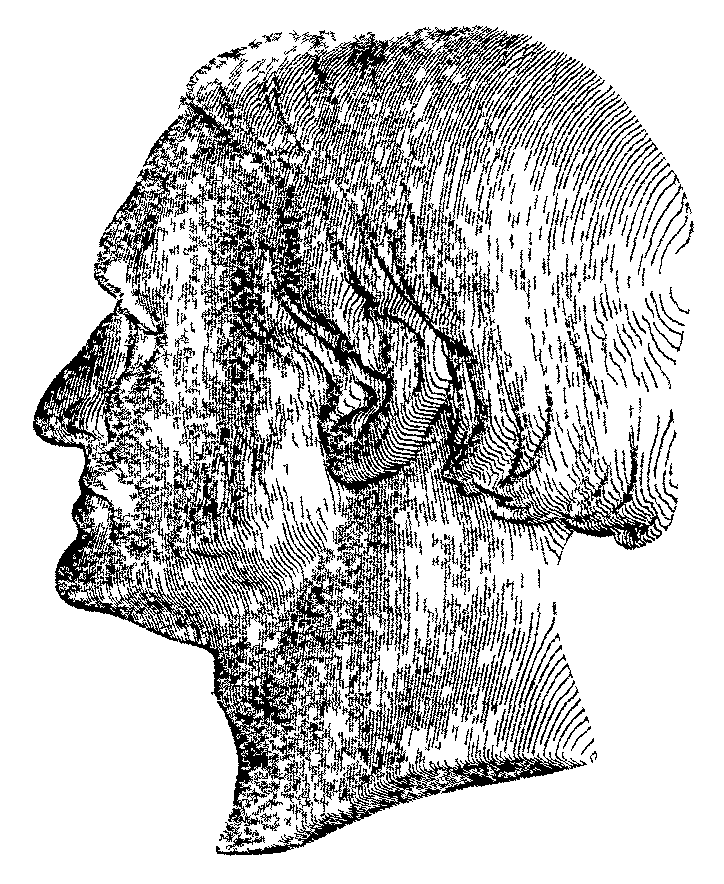
\includegraphics[width=44mm]{gauss_historical_portrait.png}\par\vspace{18mm}
{\footnotesize HERAUSGEGEBEN}\par\vspace{3mm}
{\scriptsize VON DER}\par\vspace{3mm}
{\small KÖNIGLICHEN GESELLSCHAFT DER WISSENSCHAFTEN}\par\vspace{3mm}
{\scriptsize ZU}\par\vspace{4mm}
{\large\textls[180]{GÖTTINGEN.}}\par\vspace{3mm}
{\small IN COMMISSION BEI B. G. TEUBNER IN LEIPZIG.}\par\vspace{3mm}
{\small 1903.}
\end{center}
\clearpage\null
\endgroup

\clearpage
\begin{center}
{\Large BESTIMMUNG}\par\vspace{8mm}
{\small DES}\par\vspace{8mm}
{\LARGE\textls[100]{BREITENUNTERSCHIEDES}}\par\vspace{8mm}
{\small ZWISCHEN DEN}\par\vspace{7mm}
{\large STERNWARTEN VON GÖTTINGEN UND ALTONA}\par\vspace{7mm}
{\small DURCH}\par\vspace{7mm}
{\normalsize BEOBACHTUNGEN AM RAMSDENSCHEN ZENITHSECTOR}\par\vspace{7mm}
{\small VON}\par\vspace{7mm}
{\large\textls[100]{CARL FRIEDRICH GAUSS,}}\par\smallskip
{\scriptsize
RITTER DES GUELPHEN- UND DANNEBROG-ORDENS; K. GROSSBR. HANNOVERSCHEM HOFRATH;\\
PROFESSOR DER ASTRONOMIE UND DIRECTOR DER STERNWARTE IN GÖTTINGEN;\\
MITGLIED DER AKADEMIEN UND SOCIETÄTEN VON BERLIN, COPENHAGEN, EDINBURG, GÖTTINGEN,\\
LONDON, MÜNCHEN, NEAPEL, PARIS, PETERSBURG, STOCKHOLM,\\
DER AMERIKANISCHEN, ITALIENISCHEN, KURLÄNDISCHEN, LONDONER ASTRONOMISCHEN U. A.
}\par\vspace{15mm}
\rule{.35\textwidth}{.4pt}\par\medskip
{\large\textls[170]{GÖTTINGEN,}}\par\medskip
BEI VANDENHOECK UND RUPRECHT.\par\medskip
1828.
\end{center}
\vfill\noindent IX.\hfill 1\par

\clearpage
\null

\clearpage
\begin{center}
{\LARGE\textls[170]{INHALT.}}\par\medskip
\rule{.09\textwidth}{.4pt}
\end{center}
\noindent Einleitung\dotfill S.\quad 5\par
\noindent\makebox[8mm][r]{I.}\quad Die beobachteten Sterne.\dotfill \quotedblbase\quad 8\par
\noindent\makebox[8mm][r]{II.}\quad Die Beobachtungen\dotfill \quotedblbase\quad 10\par
\noindent\makebox[8mm][r]{III.}\quad Resultate\dotfill \quotedblbase\quad 29\par
\noindent\hspace*{12mm}\begin{minipage}{\dimexpr\textwidth-24mm\relax}
Einfachste Combination der Beobachtungen zur Bestimmung des
Breitenunterschiedes, Art.\ 1. Genauigkeit der Beobachtungen,
Art.\ 2. Collimationsfehler, Art.\ 3. Absolut vortheilhafteste Combination
der Beobachtungen, Art.\ 4---7. Berücksichtigung der
unregelmässigen Theilungsfehler, Art.\ 8---11. Lage der Beobachtungsplätze,
Art.\ 12. Bestimmung der absoluten Polhöhe der
Göttinger Sternwarte aus Beobachtungen des Nordsterns am
\textsc{Reichenbach}schen Meridiankreise, Art.\ 13---17. Endresultat der
hannoverschen Gradmessung, Art.\ 18---20. Vergleichung der
Declinationen der beobachteten Zenithsterne mit \textsc{Bradleys} und
\textsc{Piazzis} Bestimmungen, Art.\ 21.
\end{minipage}\par
\noindent\makebox[8mm][r]{IV.}\quad Breitenbestimmung der Sternwarte Seeberg\dotfill \quotedblbase\quad 52\par
\noindent Zusatz zu [Art.\ 20] S.\ 48\dotfill \quotedblbase\quad 56\par
\begin{center}\rule{.23\textwidth}{.4pt}\end{center}
\vfill\begin{flushright}$1^{\ast}$\end{flushright}

\clearpage
\null

\clearpage
\vspace*{12mm}
\begin{center}
{\large BESTIMMUNG DES BREITENUNTERSCHIEDES}\par\medskip
{\small ZWISCHEN}\par\medskip
{\large DEN STERNWARTEN VON GÖTTINGEN UND ALTONA\\
DURCH BEOBACHTUNGEN\\
AM RAMSDENSCHEN ZENITHSECTOR.}\par\medskip
\rule{.12\textwidth}{.4pt}\par\bigskip
{\large EINLEITUNG.}
\end{center}

Durch die von mir in den Jahren 1821---1824 durch das Königreich Hannover
längs des Meridians von Göttingen geführte Dreieckskette sind die
Sternwarten von Göttingen und Altona auf das Genaueste trigonometrisch mit
einander verbunden. Diese Messungen werden in Zukunft ausführlich bekannt
gemacht werden: hier wird nur bemerkt, dass die absoluten Grössen
auf der von Herrn Prof.\ \textsc{Schumacher} in Holstein mit äusserster Schärfe gemessenen
Basis beruhen, mit welcher das Dreieckssystem durch die Seite
Hamburg-Hohenhorn zusammenhängt; die Orientirung gründet sich auf die
Beobachtungen am Göttinger Mittagsfernrohr, da die Sternwarte und das
nördliche Meridianzeichen selbst Dreieckspunkte sind. Die Sternwarten von
Göttingen und Altona liegen durch ein merkwürdiges Spiel des Zufalls auf
weniger als Eine Hausbreite in einerlei Meridian. Obgleich die absoluten
Polhöhen durch die Beobachtungen mit festen Meridianinstrumenten bestimmt
sind, so war es doch wichtig, den Unterschied der Breiten noch auf eine
andere Art mit einerlei Instrument zu bestimmen, und ich war so glücklich,

\clearpage
\noindent\makebox[10mm][l]{6}\parbox[t]{\dimexpr\textwidth-10mm\relax}{\centering\scriptsize BESTIMMUNG DES\,\quotedblbase\,BREITENUNTERSCHIEDES ZWISCHEN GÖTTINGEN UND ALTONA.}\par
\noindent dazu den trefflichen \textsc{Ramsden}schen Zenithsector anwenden zu können, der bekanntlich
zu ähnlichem Zweck bei der englischen Gradmessung gedient hat.
Die damit im Frühjahr 1827 von mir angestellten Beobachtungen und ihre
Resultate sind der Hauptgegenstand dieser Schrift.

Da die Beobachtungen mit diesem Instrument, wenn viele Sterne in einer
Reihe zu beobachten sind, nicht wohl ohne den Beistand eines geübten Gehülfen
gemacht werden können, so hatte Hr.\ Prof.\ \textsc{Schumacher} die Güte,
den Hrn.\ Ingenieur-Lieutenant v.\ \textsc{Nehus}[\textsuperscript{*})], unter Genehmigung Sr.\ Majestät
des Königs von Dänemark, für die Beobachtungen an beiden Plätzen damit zu
beauftragen. Dieser sehr geschickte Beobachter hat fortwährend die Ablesung
der Mikrometerschraube und die Einstellung des Lothfadens besorgt, während
ich selbst die Antritte an die Meridianfäden beobachtete und den auf den
Meridian senkrechten Faden auf die Sterne einstellte: nur in den beiden
ersten Beobachtungsnächten in Altona war jenes Geschäft von einem andern
Gehülfen besorgt; allein diese Beobachtungen sind deshalb nicht mit aufgenommen,
zumal da die Erfahrung bestätigte, dass verschiedene Personen die
Bisection der Punkte durch den Lothfaden ungleich schätzten.

Das Instrument ist durch die ausführliche von \textsc{Mudge} gegebene Beschreibung
hinlänglich bekannt. In Göttingen konnte es in der Sternwarte selbst,
unter dem östlichen Meridianspalt, aufgestellt werden. In Altona war dies
nicht thunlich; es wurde daher in dem Garten des Hrn.\ Prof.\ \textsc{Schumacher},
in welchem die dortige Sternwarte selbst liegt, unter demselben Beobachtungszelte,
welches \textsc{Mudge} in England gebraucht hat, aufgestellt. Die Solidität
der Aufstellung, auf eingerammten Pfählen, liess nichts zu wünschen übrig:
das Nivellement der Verticalaxe wurde täglich nachgesehen, und gewöhnlich
fast nichts zu ändern gefunden; dasselbe gilt von der Horizontalaxe.

Um die Ebene des Limbus in den Meridian zu bringen, wurde in Göttingen
das südliche Meridianzeichen benutzt, welches zwar in dem Meridian
des westlichen Spaltes steht, dessen Azimuth am Platze des Sectors sich aber
mit grösster Schärfe berechnen liess. In Altona konnte ein ähnliches Mittel
nicht angewandt werden: der Limbus wurde zuerst, mit Hülfe der Kenntniss
der absoluten Zeit, vermittelst eines culminirenden Sterns sehr nahe in den

\vfill\noindent\rule{.24\textwidth}{.4pt}\par
{\footnotesize\noindent [\textsuperscript{*}) Handschriftliche Bemerkung:] \textsc{Nehus} starb an zurückgetretener Grippe 1844 Apr.\ 17.\par}

\clearpage
\noindent\mbox{}\hfill EINLEITUNG.\hfill 7\par
\noindent Meridian gebracht; die Beobachtung mehrerer Sterne in der ganzen Ausdehnung
des Limbus gab dann leicht die noch nöthige kleine Correction der
Aufstellung. Da, wie schon erwähnt ist, von den am Sector culminirenden
Sternen in jeder Nacht auch die Antritte an die Meridianfäden beobachtet
wurden, und die Rectascensionen der Sterne bekannt waren, so erhielt die
richtige Aufstellung im Meridian dadurch eine fortwährende sichere Controlle,
und nur einmal war eine unbedeutende Nachhülfe erforderlich. In der Regel
wurde von einer Nacht zur andern mit der Stellung des Limbus, östlich oder
westlich, abgewechselt, und nur gegen den Schluss der Beobachtungen wurde,
um die Anzahl der Beobachtungen auf beide Lagen ziemlich gleich zu vertheilen,
von dieser Regel zuweilen abgewichen, und der Sector in Einer Nacht
ein oder mehreremale umgewandt.

Der Stand des Barometers und des innern und äussern Thermometers
wurde in jeder Nacht wenigstens dreimal, zu Anfang, in der Mitte und am
Schluss der Beobachtungen aufgezeichnet. Eben so, nach dem Vorgang von
\textsc{Mudge}, der Unterschied der Temperatur oben und unten am Sector, da deshalb
der Limbus und der Radius in ungleichem Verhältnisse verändert werden.
Dass übrigens jede andere durch die Einrichtung des Instruments vorgeschriebene
Vorsicht sorgfältig beachtet ist, z.\,B.\ das Wassergefäss, in welches das
Loth hängt, gehörig angefüllt zu erhalten, von der Mikrometerschraube so
viel thunlich dieselben Gewinde spielen zu lassen u.\ dergl., ist wohl überflüssig
besonders zu bemerken. Die Einstellung des Lothfadens auf den
obern Punkt (das Centrum des Gradbogens) wurde bei der Beobachtung jedes
Sterns von neuem unabhängig von der vorhergegangenen gemacht, und die
Einstellung auf den nächsten Theilungspunkt (oder die beiden nächsten) wurde
in der Regel mehreremale wiederholt, und aus den verschiedenen Ablesungen
der Mikrometerschraube, die meistens auf wenige Decimaltheile der Secunde
übereinstimmten, das Mittel genommen.

\begin{center}\rule{.24\textwidth}{.4pt}\end{center}

\clearpage
\vspace*{18mm}
\begin{center}
{\large I.}\par\medskip
{\Large DIE BEOBACHTETEN STERNE.}
\end{center}

Ich hatte zu Anfang 38 Sterne in schicklichen Lagen zur Beobachtung
ausgewählt, denen ich gegen den Schluss der Beobachtungen in Göttingen
noch fünf andere beifügte, weil ich besorgte, dass durch ungünstiges Wetter
der Schluss der Beobachtungen in Altona so weit verzögert werden könnte,
dass ein beträchtlicher Theil der ersten Sterne wegen der bei Tage eintretenden
Culmination nicht oft genug würde beobachtet werden können. Diese
Besorgniss bestätigte sich jedoch nur in geringem Grade, und nur ein einziger
Stern ist in Altona bloss einseitig beobachtet. Ich gebe hier die mittlere
Stellung dieser Sterne auf den Anfang des Jahrs 1827 reducirt: die Declinationen
sind die Resultate, welche die Beobachtungen am Zenithsector
selbst ergeben haben; die Rectascensionen, bei welchen für den gegenwärtigen
Zweck die allerschärfste Bestimmung unwesentlich ist, gründen sich meistens
nur auf eine einmalige Beobachtung am Meridiankreise, deren Reduction
Hr.\ \textsc{von Heiligenstein} gefälligst berechnet hat. Der Bequemlichkeit wegen
bezeichne ich die Sterne mit fortlaufenden Zahlen. Nro.\ 8, 13, 15 und 31
sind Doppelsterne; bei dem ersten ist immer der nachfolgende Stern, bei den
beiden folgenden die Mitte eingestellt; bei Nro.\ 31 ist der Nebenstern so
klein, dass er im Fernrohr des Sectors, selbst bei versuchsweise verdunkeltem
Felde, immer unsichtbar blieb, obgleich er von Hrn.\ Prof.\ \textsc{Schumacher} im
lichtstärkern Fernrohr des \textsc{Reichenbach}schen Meridiankreises sofort bemerkt
wurde, ohne dass uns damals bekannt war, dass schon andere Astronomen
diesen Doppelstern als solchen erkannt hatten.

\clearpage
\noindent\parbox[t]{\dimexpr\textwidth-10mm\relax}{\centering\scriptsize BESTIMMUNG DES BREITENUNTERSCHIEDES ETC.\quad I.\quad DIE BEOBACHTETEN STERNE.}\makebox[10mm][r]{9}\par
\begin{center}
\begin{minipage}[t]{.49\textwidth}\centering
{\scriptsize\setlength{\tabcolsep}{1.2pt}\renewcommand{\arraystretch}{1.2}\begin{tabular}{r|l|rrr|rrr|}
\multicolumn{2}{c|}{Bezeichnung}&\multicolumn{3}{c|}{G. Aufst. 1827}&\multicolumn{3}{c|}{Declin. 1827}\\\hline
1&24 Canum&$13^{\mathrm h}$&$27^{\mathrm m}$&$22^{\mathrm s}{,}39$&$49^\circ$&$54'$&$11''{,}62$\\
2&83 Ursae&&$34$&$9{,}77$&$55$&$33$&$34{,}98$\\
3&$\eta$ Ursae&&$40$&$42{,}86$&$50$&$10$&$46{,}20$\\
4&86 Ursae&&$47$&$28{,}48$&$54$&$34$&$55{,}55$\\
5&&&$50$&$45{,}55$&$55$&$25$&$59{,}22$\\
6&P. 13. 289&&$55$&$19{,}44$&$46$&$35$&$39{,}14$\\
7&13 Bootis&$14$&$1$&$49{,}02$&$50$&$16$&$43{,}44$\\
8&$\varkappa$ Bootis seq.&&$7$&$16{,}93$&$52$&$36$&$7{,}47$\\
9&P. 14. 56&&$12$&$5{,}39$&$56$&$13$&$36{,}51$\\
10&$\theta$ Bootis&&$19$&$18{,}40$&$52$&$39$&$12{,}05$\\
11&P. 14. 131&&$27$&$50{,}42$&$53$&$39$&$33{,}02$\\
12&P. 14. 164&&$35$&$24{,}18$&$52$&$58$&$55{,}66$\\
13&39 Bootis med.&&$43$&$48{,}37$&$49$&$26$&$9{,}46$\\
14&P. 14. 235&&$50$&$38{,}71$&$50$&$20$&$22{,}49$\\
15&44 Bootis med.&&$58$&$5{,}30$&$48$&$19$&$52{,}47$\\
16&&$15$&$7$&$8{,}12$&$49$&$13$&$46{,}68$\\
17&P. 15. 39&&$10$&$33{,}95$&$51$&$34$&$53{,}72$\\
18&&&$15$&$0{,}55$&$52$&$35$&$5{,}87$\\
19&&&$21$&$50{,}88$&$54$&$37$&$34{,}87$\\
20&&&$30$&$42{,}13$&$54$&$29$&$54{,}30$\\
21&&&$38$&$9{,}07$&$52$&$54$&$37{,}09$\\
22&&&$42$&$14{,}32$&$46$&$16$&$4{,}70$\\
\end{tabular}}\end{minipage}\hfill
\begin{minipage}[t]{.49\textwidth}\centering
{\scriptsize\setlength{\tabcolsep}{1.2pt}\renewcommand{\arraystretch}{1.2}\begin{tabular}{r|l|rrr|rrr}
\multicolumn{2}{c|}{Bezeichnung}&\multicolumn{3}{c|}{G. Aufst. 1827}&\multicolumn{3}{c}{Declin. 1827}\\\hline
23&&$15^{\mathrm h}$&$48^{\mathrm m}$&$16^{\mathrm s}{,}24$&$56^\circ$&$20'$&$27''{,}00$\\
24&&&$54$&$10{,}23$&$50$&$22$&$39{,}41$\\
25&$\theta$ Draconis&&$58$&$39{,}70$&$59$&$1$&$47{,}14$\\
26&&$16$&$4$&$24{,}06$&$50$&$38$&$13{,}12$\\
27&P. 16. 33&&$7$&$24{,}92$&$46$&$20$&$17{,}04$\\
28&P. 16. 56&&$11$&$34{,}31$&$53$&$40$&$13{,}41$\\
29&&&$16$&$2{,}19$&$52$&$27$&$11{,}06$\\
30&&&$20$&$38{,}75$&$55$&$36$&$4{,}73$\\
31&&&$26$&$34{,}90$&$45$&$58$&$5{,}85$\\
32&16 Draconis&&$32$&$6{,}42$&$53$&$15$&$3{,}64$\\
33&&&$37$&$53{,}85$&$50$&$16$&$13{,}67$\\
34&&&$42$&$1{,}51$&$57$&$5$&$37{,}79$\\
35&&&$45$&$2{,}26$&$46$&$56$&$48{,}53$\\
36&P. 16. 253&&$49$&$21{,}51$&$46$&$49$&$22{,}01$\\
37&P. 16. 291&&$56$&$11{,}73$&$56$&$56$&$42{,}35$\\
38&P. 16. 310&$17$&$0$&$15{,}10$&$49$&$2$&$47{,}09$\\
39&P. 17. 20&&$4$&$23{,}12$&$58$&$29$&$49{,}33$\\
40&P. 17. 38&&$8$&$1{,}46$&$56$&$52$&$21{,}74$\\
41&74 Herculis&&$15$&$28{,}30$&$46$&$24$&$52{,}90$\\
42&P. 17. 120&&$20$&$53{,}56$&$57$&$10$&$13{,}11$\\
43&$\beta$ Draconis&&$26$&$31{,}90$&$52$&$25$&$57{,}91$\\
&&&&&&&\\
\end{tabular}}\end{minipage}
\end{center}
\begin{center}\rule{.24\textwidth}{.4pt}\end{center}

\clearpage
\vspace*{18mm}
\begin{center}
{\large II.}\par\medskip
{\Large DIE BEOBACHTUNGEN.}
\end{center}

Ein vollständiger Abdruck des Tagebuchs in seiner ursprünglichen Gestalt,
welcher die Stärke dieser Schrift mehr als verdoppelt haben würde, hat
mir überflüssig geschienen: ich gebe daher die Beobachtungen sogleich nach
den Sternen geordnet.

Die erste Columne enthält die Zenithdistanzen, wie das Instrument sie
gegeben hat, d.\,i.\ die blosse Reduction der Ablesung. Nördliche Zenithdistanzen
sind als positiv, südliche als negativ betrachtet.

Die zweite Columne gibt die Vereinigung der Refraction mit der Wirkung
der ungleichen Ausdehnung des Instruments wegen Ungleichheit der
obern und untern Temperatur: die äussersten vorgekommenen Unterschiede
waren $+1^\circ{,}2$ Réaum.\ (das obere Thermometer höher) und $-0^\circ{,}6$. Um ein
reines Resultat zur Beurtheilung der Übereinstimmung der Beobachtungen
unter sich zu erhalten, habe ich die Mühe nicht gescheut, den Betrag für
jede einzelne Beobachtung zu berechnen, wobei jedoch einige kleine sich
leicht darbietende Rechnungsvortheile benutzt sind.

Die dritte Columne enthält die Reduction auf den mittlern Ort für den
Anfang des Jahrs wegen Aberration, Nutation und Praecession, wozu bei
einigen Sternen noch die eigene Bewegung gesetzt ist: es ist nemlich die jährliche
eigene Bewegung in Declination angenommen
\begin{center}
\begin{tabular}{@{}lr@{\quad}c@{\quad}l@{}}
für&10&.\ .\ .\ .\ .\ .\ .&$-0''{,}42$\\
&25&.\ .\ .\ .\ .\ .\ .&$+0{,}33$\\
&37&.\ .\ .\ .\ .\ .\ .&$+0{,}38$.
\end{tabular}
\end{center}

\clearpage
\noindent\parbox[t]{\dimexpr\textwidth-10mm\relax}{\centering\scriptsize BESTIMMUNG DES BREITENUNTERSCHIEDES ETC.\quad II.\quad DIE BEOBACHTUNGEN.}\makebox[10mm][r]{11}\par
\noindent Bei den beiden ersten Sternen ist die eigene Bewegung längst entschieden;
bei 37 zeigt sie sich durch Vergleichung mit \textsc{Piazzis} Bestimmung so, dass,
die Richtigkeit der letztern vorausgesetzt, sie nicht bezweifelt werden kann\textsuperscript{*}).
Der Berechnung der Aberration, Nutation und Praecession liegen \textsc{Bailys}
schätzbare Tafeln zum Grunde, nach denen für jeden Stern eine Ephemeride
von 10 zu 10 Tagen, unter Beihülfe der Hrn.\ v.\ \textsc{Nehus} und \textsc{Petersen}, berechnet,
und in diese mit Berücksichtigung der zweiten Differenzen interpolirt
wurde.

Die vierte Columne enthält endlich die Summe der drei ersten, also die
wahre nur noch mit dem Collimationsfehler behaftete Zenithdistanz für die
mittlere Stellung zu Anfang des Jahrs 1827, wie sie sich aus jeder einzelnen
Beobachtung ergibt.

\medskip\noindent\rule{.24\textwidth}{.4pt}\par
{\footnotesize
\noindent\textsuperscript{*}) Die Richtigkeit von \textsc{Piazzis} Bestimmung dieses Sterns, auf 8 Beobachtungen gegründet, erhält
durch die nahe Übereinstimmung mit der Angabe der ältern Ausgabe seines Verzeichnisses von 1803,
welche auf 6 Beobachtungen beruhte, eine Bestätigung; die genaue Grösse der eigenen Bewegung bleibt
aber deswegen noch etwas ungewiss, weil das Jahr unbekannt ist, welches dem Mittel der Beobachtungen
entspricht. Es ist merkwürdig, diese nicht unbeträchtliche eigene Bewegung bei einem Stern der 7.\ Grösse
zu finden. Auch Nro.\ 11 scheint in dieser Beziehung die Aufmerksamkeit der Astronomen zu verdienen.\par}
\begin{center}\rule{.24\textwidth}{.4pt}\end{center}

\begingroup
\setlength{\arraycolsep}{2.2pt}
\setlength{\tabcolsep}{0pt}
\renewcommand{\arraystretch}{1.00}
\def\ixStar#1{\par\noindent\hfill{\normalsize\textls[80]{#1}}\hfill\null\par\smallskip}
\footnotesize

% Printed 12; principal PDF 19; Google PDF 23.
\par\clearpage
\noindent\makebox[12mm][l]{\fontsize{13}{16}\selectfont 12}\parbox[t]{\dimexpr\linewidth-24mm\relax}{\centering\scriptsize\bfseries BESTIMMUNG DES BREITENUNTERSCHIEDES ZWISCHEN GÖTTINGEN UND ALTONA.}\makebox[12mm][r]{}\par\medskip

\vspace*{.19\textheight}
\ixStar{1.\quad (24 Canum Venaticorum)}
\noindent\begin{tabular}{@{}c@{\hspace{.4em}\vrule width .65pt\hspace{.4em}}c@{}}
\multicolumn{1}{@{}c@{\hspace{.8em}}}{\makebox[.48\linewidth][c]{\normalsize Göttingen.\quad Limbus Ost.}} &
\multicolumn{1}{@{}c@{}}{\makebox[.48\linewidth][c]{\normalsize Göttingen.\quad Limbus West.}} \\[.18ex]
\(\begin{array}[t]{@{}r|r|r|r|r@{}}
\text{Apr.}\enspace 5 & -1^\circ\,37'\,52''{,}62 & -1''{,}66 & +13''{,}34 & -1^\circ\,37'\,40''{,}94\\
17 & 47{,}75 & -1{,}62 & +10{,}12 & 39{,}25\\
28 & 46{,}01 & -1{,}61 & +7{,}15 & 40{,}47\\
29 & 44{,}57 & -1{,}61 & +6{,}88 & 39{,}30\\
 & & & & \\
\cline{5-5}
\multicolumn{4}{r}{\text{Mittel aus 4 Beobachtungen}} & -1\,37\,39{,}99
\end{array}\)
&
\(\begin{array}[t]{@{}r|r|r|r|r@{}}
\text{Apr.}\enspace 11 & -1^\circ\,37'\,43''{,}60 & -1''{,}59 & +11''{,}75 & -1^\circ\,37'\,33''{,}44\\
20 & 40{,}36 & -1{,}62 & +9{,}31 & 32{,}67\\
27 & 37{,}29 & -1{,}67 & +7{,}41 & 31{,}55\\
30 & 36{,}84 & -1{,}55 & +6{,}62 & 31{,}77\\
\text{Mai}\enspace 14 & 34{,}23 & -1{,}60 & +3{,}02 & 32{,}81\\
\cline{5-5}
\multicolumn{4}{r}{\text{Mittel aus 5 Beobachtungen}} & -1\,37\,32{,}45
\end{array}\)
\end{tabular}\par\medskip
\noindent\begin{tabular}{@{}c@{\hspace{.4em}\vrule width .65pt\hspace{.4em}}c@{}}
\multicolumn{1}{@{}c@{\hspace{.8em}}}{\makebox[.48\linewidth][c]{\normalsize Altona.\quad Limbus Ost.}} &
\multicolumn{1}{@{}c@{}}{\makebox[.48\linewidth][c]{\normalsize Altona.\quad Limbus West.}} \\[.18ex]
\(\begin{array}[t]{@{}r|r|r|r|r@{}}
\text{Jun.}\enspace 4 & -3^\circ\,38'\,29''{,}77 & -3''{,}68 & -1''{,}53 & -3^\circ\,38'\,34''{,}98\\
10 & 26{,}44 & -3{,}58 & -2{,}57 & 32{,}59\\
11 & 28{,}52 & -3{,}56 & -2{,}73 & 34{,}81\\
13 & 29{,}85 & -3{,}53 & -3{,}03 & 36{,}41\\
15 & 26{,}74 & -3{,}44 & -3{,}33 & 33{,}51\\
\cline{5-5}
\multicolumn{4}{r}{\text{Mittel aus 5 Beobachtungen}} & -3\,38\,34{,}46
\end{array}\)
&
\(\begin{array}[t]{@{}r|r|r|r|r@{}}
\text{Jun.}\enspace 3 & -3^\circ\,38'\,25''{,}37 & -3''{,}69 & -1''{,}35 & -3^\circ\,38'\,30''{,}41\\
6 & 25{,}44 & -3{,}59 & -1{,}89 & 30{,}92\\
9 & 25{,}32 & -3{,}60 & -2{,}41 & 31{,}33\\
12 & 26{,}07 & -3{,}54 & -2{,}89 & 32{,}50\\
 & & & & \\
\cline{5-5}
\multicolumn{4}{r}{\text{Mittel aus 4 Beobachtungen}} & -3\,38\,31{,}29
\end{array}\)
\end{tabular}\par\medskip
\bigskip
\ixStar{2.\quad (83 Ursae maioris)}
\noindent\begin{tabular}{@{}c@{\hspace{.4em}\vrule width .65pt\hspace{.4em}}c@{}}
\multicolumn{1}{@{}c@{\hspace{.8em}}}{\makebox[.48\linewidth][c]{\normalsize Göttingen.\quad Limbus Ost.}} &
\multicolumn{1}{@{}c@{}}{\makebox[.48\linewidth][c]{\normalsize Göttingen.\quad Limbus West.}} \\[.18ex]
\(\begin{array}[t]{@{}r|r|r|r|r@{}}
\text{Apr.}\enspace 5 & +4^\circ\,1'\,26''{,}05 & +4''{,}10 & +12''{,}99 & +4^\circ\,1'\,43''{,}14\\
7 & 27{,}08 & +4{,}02 & +12{,}42 & 43{,}52\\
9 & 28{,}85 & +3{,}99 & +11{,}86 & 44{,}70\\
17 & 30{,}25 & +4{,}00 & +9{,}58 & 43{,}83\\
28 & 33{,}16 & +3{,}98 & +6{,}43 & 43{,}57\\
29 & 34{,}26 & +3{,}97 & +6{,}14 & 44{,}37\\
 & & & & \\
\cline{5-5}
\multicolumn{4}{r}{\text{Mittel aus 6 Beobachtungen}} & +4\,1\,43{,}86
\end{array}\)
&
\(\begin{array}[t]{@{}r|r|r|r|r@{}}
\text{Apr.}\enspace 6 & +4^\circ\,1'\,34''{,}39 & +4''{,}07 & +12''{,}71 & +4^\circ\,1'\,51''{,}17\\
8 & 33{,}81 & +3{,}97 & +12{,}14 & 49{,}92\\
11 & 35{,}49 & +3{,}93 & +11{,}30 & 50{,}72\\
20 & 36{,}86 & +4{,}00 & +8{,}73 & 49{,}59\\
27 & 39{,}97 & +4{,}12 & +6{,}71 & 50{,}80\\
30 & 40{,}94 & +3{,}80 & +5{,}86 & 50{,}60\\
\text{Mai}\enspace 14 & 46{,}33 & +3{,}96 & +2{,}06 & 52{,}35\\
\cline{5-5}
\multicolumn{4}{r}{\text{Mittel aus 7 Beobachtungen}} & +4\,1\,50{,}74
\end{array}\)
\end{tabular}\par\medskip
\noindent\begin{tabular}{@{}c@{\hspace{.4em}\vrule width .65pt\hspace{.4em}}c@{}}
\multicolumn{1}{@{}c@{\hspace{.8em}}}{\makebox[.48\linewidth][c]{\normalsize Altona.\quad Limbus Ost.}} &
\multicolumn{1}{@{}c@{}}{\makebox[.48\linewidth][c]{\normalsize Altona:\quad Limbus West.}} \\[.18ex]
\(\begin{array}[t]{@{}r|r|r|r|r@{}}
\text{Jun.}\enspace 4 & +2^\circ\,0'\,49''{,}03 & +2''{,}04 & -2''{,}72 & +2^\circ\,0'\,48''{,}35\\
7 & 51{,}21 & +2{,}01 & -3{,}28 & 49{,}94\\
10 & 49{,}21 & +1{,}98 & -3{,}80 & 47{,}39\\
11 & 50{,}31 & +1{,}97 & -3{,}97 & 48{,}31\\
13 & 52{,}49 & +1{,}95 & -4{,}29 & 50{,}15\\
15 & 52{,}79 & +1{,}90 & -4{,}59 & 50{,}10\\
\cline{5-5}
\multicolumn{4}{r}{\text{Mittel aus 6 Beobachtungen}} & +2\,0\,49{,}04
\end{array}\)
&
\(\begin{array}[t]{@{}r|r|r|r|r@{}}
\text{Jun.}\enspace 3 & +2^\circ\,0'\,51''{,}64 & +2''{,}05 & -2''{,}52 & +2^\circ\,0'\,51''{,}17\\
6 & 51{,}71 & +1{,}99 & -3{,}10 & 50{,}60\\
9 & 53{,}71 & +2{,}00 & -3{,}63 & 52{,}08\\
12 & 53{,}96 & +1{,}96 & -4{,}13 & 51{,}79\\
 & & & & \\
 & & & & \\
\cline{5-5}
\multicolumn{4}{r}{\text{Mittel aus 4 Beobachtungen}} & +2\,0\,51{,}41
\end{array}\)
\end{tabular}\par\medskip

% Printed 13; principal PDF 20; Google PDF 24.
\par\clearpage
\noindent\makebox[12mm][l]{}\makebox[\dimexpr\linewidth-24mm\relax][c]{\small\textbf{II.\quad DIE BEOBACHTUNGEN.}}\makebox[12mm][r]{\fontsize{13}{16}\selectfont 13}\par\medskip

\ixStar{3.\quad (\(\eta\) Ursae maioris)}
\noindent\begin{tabular}{@{}c@{\hspace{.4em}\vrule width .65pt\hspace{.4em}}c@{}}
\multicolumn{1}{@{}c@{\hspace{.8em}}}{\makebox[.48\linewidth][c]{\normalsize Göttingen.\quad Limbus Ost.}} &
\multicolumn{1}{@{}c@{}}{\makebox[.48\linewidth][c]{\normalsize Göttingen.\quad Limbus West.}} \\[.18ex]
\(\begin{array}[t]{@{}r|r|r|r|r@{}}
\text{Apr.}\enspace 5 & -1^\circ\,21'\,18''{,}73 & -1''{,}38 & +13''{,}58 & -1^\circ\,21'\,6''{,}53\\
7 & 16{,}66 & -1{,}35 & +13{,}05 & 4{,}96\\
9 & 16{,}23 & -1{,}34 & +12{,}52 & 5{,}05\\
17 & 12{,}25 & -1{,}35 & +10{,}35 & 3{,}25\\
28 & 11{,}32 & -1{,}34 & +7{,}33 & 5{,}33\\
29 & 10{,}62 & -1{,}34 & +7{,}05 & 4{,}91\\
 & & & & \\
\cline{5-5}
\multicolumn{4}{r}{\text{Mittel aus 6 Beobachtungen}} & -1\,21\,5{,}00
\end{array}\)
&
\(\begin{array}[t]{@{}r|r|r|r|r@{}}
\text{Apr.}\enspace 6 & -1^\circ\,21'\,11''{,}05 & -1''{,}37 & +13''{,}32 & -1^\circ\,20'\,59''{,}10\\
8 & 9{,}52 & -1{,}34 & +12{,}78 & 58{,}08\\
11 & 7{,}31 & -1{,}32 & +11{,}99 & 56{,}64\\
20 & 7{,}01 & -1{,}35 & +9{,}53 & 58{,}83\\
27 & 3{,}44 & -1{,}39 & +7{,}60 & 57{,}23\\
30 & 2{,}98 & -1{,}29 & +6{,}78 & 57{,}49\\
\text{Mai}\enspace 14 & -1\,20\,57{,}75 & -1{,}33 & +3{,}08 & 56{,}00\\
\cline{5-5}
\multicolumn{4}{r}{\text{Mittel aus 7 Beobachtungen}} & -1\,20\,57{,}62
\end{array}\)
\end{tabular}\par\medskip
\noindent\begin{tabular}{@{}c@{\hspace{.4em}\vrule width .65pt\hspace{.4em}}c@{}}
\multicolumn{1}{@{}c@{\hspace{.8em}}}{\makebox[.48\linewidth][c]{\normalsize Altona.\quad Limbus Ost.}} &
\multicolumn{1}{@{}c@{}}{\makebox[.48\linewidth][c]{\normalsize Altona.\quad Limbus West.}} \\[.18ex]
\(\begin{array}[t]{@{}r|r|r|r|r@{}}
\text{Jun.}\enspace 4 & -3^\circ\,21'\,55''{,}72 & -3''{,}40 & -1''{,}71 & -3^\circ\,21'\,60''{,}83\\
7 & 54{,}87 & -3{,}37 & -2{,}32 & 60{,}56\\
10 & 53{,}29 & -3{,}32 & -2{,}83 & 59{,}44\\
11 & 54{,}89 & -3{,}30 & -3{,}00 & 61{,}19\\
13 & 52{,}91 & -3{,}26 & -3{,}34 & 59{,}51\\
15 & 53{,}54 & -3{,}18 & -3{,}66 & 60{,}38\\
\cline{5-5}
\multicolumn{4}{r}{\text{Mittel aus 6 Beobachtungen}} & -3\,22\,0{,}32
\end{array}\)
&
\(\begin{array}[t]{@{}r|r|r|r|r@{}}
\text{Jun.}\enspace 6 & -3^\circ\,21'\,52''{,}11 & -3''{,}32 & -2''{,}10 & -3^\circ\,21'\,57''{,}53\\
9 & 51{,}86 & -3{,}34 & -2{,}65 & 57{,}85\\
12 & 49{,}73 & -3{,}29 & -3{,}17 & 56{,}19\\
14 & 50{,}27 & -3{,}33 & -3{,}51 & 57{,}11\\
22 & 47{,}73 & -3{,}26 & -4{,}66 & 55{,}65\\
27 & 49{,}23 & -3{,}24 & -5{,}29 & 57{,}76\\
\cline{5-5}
\multicolumn{4}{r}{\text{Mittel aus 6 Beobachtungen}} & -3\,21\,57{,}02
\end{array}\)
\end{tabular}\par\medskip
\ixStar{4.\quad (86 Ursae maioris)}
\noindent\begin{tabular}{@{}c@{\hspace{.4em}\vrule width .65pt\hspace{.4em}}c@{}}
\multicolumn{1}{@{}c@{\hspace{.8em}}}{\makebox[.48\linewidth][c]{\normalsize Göttingen.\quad Limbus Ost.}} &
\multicolumn{1}{@{}c@{}}{\makebox[.48\linewidth][c]{\normalsize Göttingen.\quad Limbus West.}} \\[.18ex]
\(\begin{array}[t]{@{}r|r|r|r|r@{}}
\text{Apr.}\enspace 5 & +3^\circ\,2'\,46''{,}67 & +3''{,}10 & +13''{,}40 & +3^\circ\,3'\,3''{,}17\\
7 & 46{,}47 & +3{,}05 & +12{,}84 & 2{,}36\\
9 & 48{,}07 & +3{,}02 & +12{,}29 & 3{,}38\\
17 & 51{,}65 & +3{,}04 & +10{,}02 & 4{,}71\\
28 & 53{,}35 & +3{,}02 & +6{,}85 & 3{,}22\\
29 & 54{,}69 & +3{,}01 & +6{,}56 & 4{,}26\\
\cline{5-5}
\multicolumn{4}{r}{\text{Mittel aus 6 Beobachtungen}} & +3\,3\,3{,}52
\end{array}\)
&
\(\begin{array}[t]{@{}r|r|r|r|r@{}}
\text{Apr.}\enspace 6 & +3^\circ\,2'\,54''{,}56 & +3''{,}08 & +13''{,}12 & +3^\circ\,3'\,10''{,}76\\
8 & 54{,}79 & +3{,}01 & +12{,}56 & 10{,}36\\
11 & 54{,}86 & +2{,}98 & +11{,}73 & 9{,}57\\
20 & 58{,}61 & +3{,}04 & +9{,}16 & 10{,}81\\
27 & 63{,}17 & +3{,}12 & +7{,}13 & 13{,}42\\
30 & 62{,}11 & +2{,}92 & +6{,}27 & 11{,}30\\
\cline{5-5}
\multicolumn{4}{r}{\text{Mittel aus 6 Beobachtungen}} & +3\,3\,11{,}04
\end{array}\)
\end{tabular}\par\medskip
\noindent\begin{tabular}{@{}c@{\hspace{.4em}\vrule width .65pt\hspace{.4em}}c@{}}
\multicolumn{1}{@{}c@{\hspace{.8em}}}{\makebox[.48\linewidth][c]{\normalsize Altona.\quad Limbus Ost.}} &
\multicolumn{1}{@{}c@{}}{\makebox[.48\linewidth][c]{\normalsize Altona.\quad Limbus West.}} \\[.18ex]
\(\begin{array}[t]{@{}r|r|r|r|r@{}}
\text{Jun.}\enspace 4 & +1^\circ\,2'\,10''{,}59 & +1''{,}05 & -2''{,}61 & +1^\circ\,2'\,9''{,}03\\
7 & 13{,}02 & +1{,}04 & -3{,}22 & 10{,}84\\
10 & 12{,}92 & +1{,}03 & -3{,}78 & 10{,}17\\
11 & 13{,}73 & +1{,}02 & -3{,}96 & 10{,}79\\
13 & 15{,}16 & +1{,}01 & -4{,}31 & 11{,}86\\
15 & 14{,}13 & +0{,}98 & -4{,}65 & 10{,}46\\
\cline{5-5}
\multicolumn{4}{r}{\text{Mittel aus 6 Beobachtungen}} & +1\,2\,10{,}52
\end{array}\)
&
\(\begin{array}[t]{@{}r|r|r|r|r@{}}
\text{Jun.}\enspace 6 & +1^\circ\,2'\,14''{,}23 & +1''{,}03 & -3''{,}02 & +1^\circ\,2'\,12''{,}24\\
9 & 15{,}43 & +1{,}03 & -3{,}60 & 12{,}86\\
12 & 15{,}05 & +1{,}01 & -4{,}14 & 11{,}92\\
 & & & & \\
 & & & & \\
 & & & & \\
\cline{5-5}
\multicolumn{4}{r}{\text{Mittel aus 3 Beobachtungen}} & +1\,2\,12{,}34
\end{array}\)
\end{tabular}\par\medskip
\ixStar{5.}
\noindent\begin{tabular}{@{}c@{\hspace{.4em}\vrule width .65pt\hspace{.4em}}c@{}}
\multicolumn{1}{@{}c@{\hspace{.8em}}}{\makebox[.48\linewidth][c]{\normalsize Göttingen.\quad Limbus Ost.}} &
\multicolumn{1}{@{}c@{}}{\makebox[.48\linewidth][c]{\normalsize Göttingen.\quad Limbus West.}} \\[.18ex]
\(\begin{array}[t]{@{}r|r|r|r|r@{}}
\text{Apr.}\enspace 5 & +3^\circ\,53'\,49''{,}88 & +3''{,}97 & +13''{,}40 & +3^\circ\,54'\,7''{,}25\\
7 & 52{,}89 & +3{,}91 & +12{,}84 & 9{,}64\\
9 & 50{,}18 & +3{,}87 & +12{,}28 & 6{,}33\\
17 & 52{,}14 & +3{,}89 & +10{,}00 & 6{,}03\\
28 & 56{,}29 & +3{,}86 & +6{,}79 & 6{,}94\\
29 & 58{,}85 & +3{,}86 & +6{,}51 & 9{,}22\\
\cline{5-5}
\multicolumn{4}{r}{\text{Mittel aus 6 Beobachtungen}} & +3\,54\,7{,}57
\end{array}\)
&
\(\begin{array}[t]{@{}r|r|r|r|r@{}}
\text{Apr.}\enspace 6 & +3^\circ\,53'\,57''{,}95 & +3''{,}94 & +13''{,}12 & +3^\circ\,54'\,15''{,}01\\
8 & 61{,}17 & +3{,}85 & +12{,}56 & 17{,}58\\
11 & 57{,}64 & +3{,}82 & +11{,}72 & 13{,}18\\
27 & 64{,}01 & +4{,}00 & +7{,}08 & 15{,}09\\
30 & 65{,}16 & +3{,}74 & +6{,}22 & 15{,}12\\
\text{Mai}\enspace 7 & 66{,}07 & +3{,}93 & +4{,}22 & 14{,}22\\
\cline{5-5}
\multicolumn{4}{r}{\text{Mittel aus 6 Beobachtungen}} & +3\,54\,15{,}03
\end{array}\)
\end{tabular}\par\medskip

% Printed 14; principal PDF 21; Google PDF 25.
\par\clearpage
\noindent\makebox[12mm][l]{\fontsize{13}{16}\selectfont 14}\parbox[t]{\dimexpr\linewidth-24mm\relax}{\centering\scriptsize\bfseries BESTIMMUNG DES BREITENUNTERSCHIEDES ZWISCHEN GÖTTINGEN UND ALTONA.}\makebox[12mm][r]{}\par\medskip

\noindent\begin{tabular}{@{}c@{\hspace{.4em}\vrule width .65pt\hspace{.4em}}c@{}}
\multicolumn{1}{@{}c@{\hspace{.8em}}}{\makebox[.48\linewidth][c]{\normalsize Altona.\quad Limbus Ost.}} &
\multicolumn{1}{@{}c@{}}{\makebox[.48\linewidth][c]{\normalsize Altona.\quad Limbus West.}} \\[.18ex]
\(\begin{array}[t]{@{}l@{}}\text{Keine Beobachtungen.}\end{array}\)
&
\(\begin{array}[t]{@{}r|r|r|r|r@{}}
\text{Jun.}\enspace 6 & +1^\circ\,53'\,17''{,}73 & +1''{,}87 & -3''{,}19 & +1^\circ\,53'\,16''{,}41\\
9 & 17{,}78 & +1{,}88 & -3{,}78 & 15{,}88\\
\cline{5-5}
\multicolumn{4}{r}{\text{Mittel aus 2 Beobachtungen}} & +1\,53\,16{,}15
\end{array}\)
\end{tabular}\par\medskip
\ixStar{6.\quad (Piazzi 13.289)}
\noindent\begin{tabular}{@{}c@{\hspace{.4em}\vrule width .65pt\hspace{.4em}}c@{}}
\multicolumn{1}{@{}c@{\hspace{.8em}}}{\makebox[.48\linewidth][c]{\normalsize Göttingen.\quad Limbus Ost.}} &
\multicolumn{1}{@{}c@{}}{\makebox[.48\linewidth][c]{\normalsize Göttingen.\quad Limbus West.}} \\[.18ex]
\(\begin{array}[t]{@{}r|r|r|r|r@{}}
\text{Apr.}\enspace 5 & -4^\circ\,56'\,21''{,}29 & -5''{,}03 & +14''{,}06 & -4^\circ\,56'\,12''{,}26\\
7 & 20{,}29 & -4{,}96 & +13{,}56 & 11{,}69\\
9 & 18{,}73 & -4{,}90 & +13{,}06 & 10{,}57\\
17 & 17{,}63 & -4{,}93 & +10{,}98 & 11{,}58\\
28 & 14{,}83 & -4{,}90 & +8{,}03 & 11{,}70\\
29 & 16{,}60 & -4{,}89 & +7{,}76 & 13{,}73\\
\cline{5-5}
\multicolumn{4}{r}{\text{Mittel aus 6 Beobachtungen}} & -4\,56\,11{,}92
\end{array}\)
&
\(\begin{array}[t]{@{}r|r|r|r|r@{}}
\text{Apr.}\enspace 6 & -4^\circ\,56'\,14''{,}63 & -4''{,}98 & +13''{,}81 & -4^\circ\,56'\,5''{,}80\\
8 & 13{,}87 & -4{,}88 & +13{,}30 & 5{,}45\\
11 & 11{,}57 & -4{,}84 & +12{,}55 & 3{,}86\\
20 & 11{,}92 & -4{,}92 & +10{,}18 & 6{,}66\\
27 & 7{,}06 & -5{,}06 & +8{,}30 & 3{,}82\\
30 & 7{,}11 & -4{,}74 & +7{,}50 & 4{,}35\\
\cline{5-5}
\multicolumn{4}{r}{\text{Mittel aus 6 Beobachtungen}} & -4\,56\,4{,}99
\end{array}\)
\end{tabular}\par\medskip
\noindent\begin{tabular}{@{}c@{\hspace{.4em}\vrule width .65pt\hspace{.4em}}c@{}}
\multicolumn{1}{@{}c@{\hspace{.8em}}}{\makebox[.48\linewidth][c]{\normalsize Altona.\quad Limbus Ost.}} &
\multicolumn{1}{@{}c@{}}{\makebox[.48\linewidth][c]{\normalsize Altona.\quad Limbus West.}} \\[.18ex]
\(\begin{array}[t]{@{}r|r|r|r|r@{}}
\text{Jun.}\enspace 11 & -6^\circ\,56'\,59''{,}93 & -6''{,}82 & -2''{,}49 & -6^\circ\,57'\,9''{,}24\\
13 & 58{,}43 & -6{,}76 & -2{,}83 & 8{,}02\\
 & & & & \\
 & & & & \\
\cline{5-5}
\multicolumn{4}{r}{\text{Mittel aus 2 Beobachtungen}} & -6\,57\,8{,}63
\end{array}\)
&
\(\begin{array}[t]{@{}r|r|r|r|r@{}}
\text{Jun.}\enspace 3 & -6^\circ\,56'\,54''{,}66 & -6''{,}96 & -0''{,}89 & -6^\circ\,57'\,2''{,}51\\
6 & 57{,}35 & -6{,}87 & -1{,}35 & 5{,}57\\
9 & 54{,}22 & -6{,}91 & -2{,}11 & 3{,}24\\
12 & 54{,}89 & -6{,}78 & -2{,}67 & 4{,}34\\
\cline{5-5}
\multicolumn{4}{r}{\text{Mittel aus 4 Beobachtungen}} & -6\,57\,3{,}92
\end{array}\)
\end{tabular}\par\medskip
\ixStar{7.\quad (13 Bootis)}
\noindent\begin{tabular}{@{}c@{\hspace{.4em}\vrule width .65pt\hspace{.4em}}c@{}}
\multicolumn{1}{@{}c@{\hspace{.8em}}}{\makebox[.48\linewidth][c]{\normalsize Göttingen.\quad Limbus Ost.}} &
\multicolumn{1}{@{}c@{}}{\makebox[.48\linewidth][c]{\normalsize Göttingen.\quad Limbus West.}} \\[.18ex]
\(\begin{array}[t]{@{}r|r|r|r|r@{}}
\text{Apr.}\enspace 5 & -1^\circ\,15'\,21''{,}54 & -1''{,}28 & +13''{,}97 & -1^\circ\,15'\,8''{,}85\\
9 & 19{,}93 & -1{,}24 & +12{,}91 & 8{,}26\\
17 & 16{,}76 & -1{,}25 & +10{,}74 & 7{,}27\\
28 & 14{,}79 & -1{,}25 & +7{,}66 & 8{,}38\\
29 & 15{,}25 & -1{,}24 & +7{,}38 & 9{,}11\\
\text{Mai}\enspace 14 & 12{,}72 & -1{,}24 & +3{,}24 & 10{,}72\\
\cline{5-5}
\multicolumn{4}{r}{\text{Mittel aus 6 Beobachtungen}} & -1\,15\,8{,}76
\end{array}\)
&
\(\begin{array}[t]{@{}r|r|r|r|r@{}}
\text{Apr.}\enspace 6 & -1^\circ\,15'\,12''{,}87 & -1''{,}26 & +13''{,}70 & -1^\circ\,14'\,60''{,}43\\
8 & 14{,}52 & -1{,}24 & +13{,}17 & 62{,}59\\
11 & 10{,}42 & -1{,}23 & +12{,}38 & 59{,}27\\
20 & 9{,}95 & -1{,}25 & +9{,}91 & 61{,}29\\
27 & 7{,}41 & -1{,}29 & +7{,}94 & 60{,}76\\
30 & 4{,}94 & -1{,}21 & +7{,}10 & 59{,}05\\
\cline{5-5}
\multicolumn{4}{r}{\text{Mittel aus 6 Beobachtungen}} & -1\,15\,0{,}56
\end{array}\)
\end{tabular}\par\medskip
\noindent\begin{tabular}{@{}c@{\hspace{.4em}\vrule width .65pt\hspace{.4em}}c@{}}
\multicolumn{1}{@{}c@{\hspace{.8em}}}{\makebox[.48\linewidth][c]{\normalsize Altona.\quad Limbus Ost.}} &
\multicolumn{1}{@{}c@{}}{\makebox[.48\linewidth][c]{\normalsize Altona.\quad Limbus West.}} \\[.18ex]
\(\begin{array}[t]{@{}r|r|r|r|r@{}}
\text{Jun.}\enspace 4 & -3^\circ\,15'\,57''{,}95 & -3''{,}31 & -1''{,}90 & -3^\circ\,16'\,3''{,}16\\
7 & 56{,}56 & -3{,}28 & -2{,}54 & 2{,}38\\
10 & 55{,}39 & -3{,}24 & -3{,}14 & 1{,}77\\
11 & 56{,}17 & -3{,}21 & -3{,}33 & 2{,}71\\
13 & 55{,}69 & -3{,}17 & -3{,}71 & 2{,}57\\
15 & 54{,}97 & -3{,}10 & -4{,}07 & 2{,}14\\
\cline{5-5}
\multicolumn{4}{r}{\text{Mittel aus 6 Beobachtungen}} & -3\,16\,2{,}46
\end{array}\)
&
\(\begin{array}[t]{@{}r|r|r|r|r@{}}
\text{Jun.}\enspace 6 & -3^\circ\,15'\,52''{,}94 & -3''{,}23 & -2''{,}33 & -3^\circ\,15'\,58''{,}50\\
9 & 51{,}56 & -3{,}26 & -2{,}94 & 57{,}76\\
12 & 53{,}15 & -3{,}19 & -3{,}52 & 59{,}86\\
14 & 52{,}84 & -3{,}23 & -3{,}89 & 59{,}96\\
22 & 50{,}89 & -3{,}19 & -5{,}22 & 59{,}30\\
 & & & & \\
\cline{5-5}
\multicolumn{4}{r}{\text{Mittel aus 5 Beobachtungen}} & -3\,15\,59{,}08
\end{array}\)
\end{tabular}\par\medskip
\ixStar{8.\quad (\(\kappa\) Bootis sequ.)}
\noindent\begin{tabular}{@{}c@{\hspace{.4em}\vrule width .65pt\hspace{.4em}}c@{}}
\multicolumn{1}{@{}c@{\hspace{.8em}}}{\makebox[.48\linewidth][c]{\normalsize Göttingen.\quad Limbus Ost.}} &
\multicolumn{1}{@{}c@{}}{\makebox[.48\linewidth][c]{\normalsize Göttingen.\quad Limbus West.}} \\[.18ex]
\(\begin{array}[t]{@{}r|r|r|r|r@{}}
\text{Apr.}\enspace 5 & +1^\circ\,4'\,1''{,}50 & +1''{,}09 & +13''{,}92 & +1^\circ\,4'\,16''{,}51\\
7 & 0{,}10 & +1{,}07 & +13{,}39 & 14{,}56\\
9 & 1{,}25 & +1{,}06 & +12{,}85 & 15{,}16\\
17 & 5{,}21 & +1{,}07 & +10{,}62 & 16{,}90\\
28 & 6{,}18 & +1{,}06 & +7{,}47 & 14{,}71\\
29 & 6{,}24 & +1{,}06 & +7{,}18 & 14{,}48\\
\text{Mai}\enspace 14 & 10{,}32 & +1{,}05 & +2{,}92 & 14{,}29\\
\cline{5-5}
\multicolumn{4}{r}{\text{Mittel aus 7 Beobachtungen}} & +1\,4\,15{,}23
\end{array}\)
&
\(\begin{array}[t]{@{}r|r|r|r|r@{}}
\text{Apr.}\enspace 6 & +1^\circ\,4'\,7''{,}96 & +1''{,}09 & +13''{,}66 & +1^\circ\,4'\,22''{,}71\\
8 & 9{,}64 & +1{,}06 & +13{,}12 & 23{,}82\\
11 & 11{,}72 & +1{,}05 & +12{,}31 & 25{,}08\\
20 & 9{,}64 & +1{,}07 & +9{,}77 & 20{,}48\\
27 & 16{,}08 & +1{,}10 & +7{,}76 & 24{,}94\\
30 & 15{,}15 & +1{,}03 & +6{,}90 & 23{,}08\\
\text{Mai}\enspace 7 & 17{,}96 & +1{,}08 & +4{,}87 & 23{,}91\\
\cline{5-5}
\multicolumn{4}{r}{\text{Mittel aus 7 Beobachtungen}} & +1\,4\,23{,}43
\end{array}\)
\end{tabular}\par\medskip

% Printed 15; principal PDF 22; Google PDF 26.
\par\clearpage
\noindent\makebox[12mm][l]{}\makebox[\dimexpr\linewidth-24mm\relax][c]{\small\textbf{II.\quad DIE BEOBACHTUNGEN.}}\makebox[12mm][r]{\fontsize{13}{16}\selectfont 15}\par\medskip

\noindent\begin{tabular}{@{}c@{\hspace{.4em}\vrule width .65pt\hspace{.4em}}c@{}}
\multicolumn{1}{@{}c@{\hspace{.8em}}}{\makebox[.48\linewidth][c]{\normalsize Altona.\quad Limbus Ost.}} &
\multicolumn{1}{@{}c@{}}{\makebox[.48\linewidth][c]{\normalsize Altona.\quad Limbus West.}} \\[.18ex]
\(\begin{array}[t]{@{}r|r|r|r|r@{}}
\text{Jun}\enspace 4 & -0^\circ\,56'\,35''{,}42 & -0''{,}95 & -2''{,}35 & -0^\circ\,56'\,38''{,}72\\
7 & 32{,}68 & -0{,}94 & -3{,}01 & 36{,}63\\
10 & 32{,}68 & -0{,}93 & -3{,}63 & 37{,}24\\
11 & 33{,}33 & -0{,}92 & -3{,}83 & 38{,}08\\
13 & 31{,}62 & -0{,}91 & -4{,}22 & 36{,}75\\
15 & 32{,}63 & -0{,}89 & -4{,}60 & 38{,}12\\
\cline{5-5}
\multicolumn{4}{r}{\text{Mittel aus 6 Beobachtungen}} & -0\,56\,37{,}59
\end{array}\)
&
\(\begin{array}[t]{@{}r|r|r|r|r@{}}
\text{Jun.}\enspace 6 & -0^\circ\,56'\,32''{,}26 & -0''{,}93 & -2''{,}79 & -0^\circ\,56'\,35''{,}98\\
9 & 31{,}73 & -0{,}93 & -3{,}43 & 36{,}09\\
12 & 31{,}78 & -0{,}91 & -4{,}02 & 36{,}71\\
14 & 31{,}33 & -0{,}93 & -4{,}41 & 36{,}67\\
22 & 27{,}35 & -0{,}92 & -5{,}79 & 34{,}06\\
27 & 27{,}88 & -0{,}91 & -6{,}51 & 35{,}30\\
\cline{5-5}
\multicolumn{4}{r}{\text{Mittel aus 6 Beobachtungen}} & -0\,56\,35{,}80
\end{array}\)
\end{tabular}\par\medskip
\ixStar{9.\quad (Piazzi 14.56)}
\noindent\begin{tabular}{@{}c@{\hspace{.4em}\vrule width .65pt\hspace{.4em}}c@{}}
\multicolumn{1}{@{}c@{\hspace{.8em}}}{\makebox[.48\linewidth][c]{\normalsize Göttingen.\quad Limbus Ost.}} &
\multicolumn{1}{@{}c@{}}{\makebox[.48\linewidth][c]{\normalsize Göttingen.\quad Limbus West.}} \\[.18ex]
\(\begin{array}[t]{@{}r|r|r|r|r@{}}
\text{Apr.}\enspace 5 & +4^\circ\,41'\,28''{,}15 & +4''{,}78 & +13''{,}81 & +4^\circ\,41'\,46''{,}74\\
7 & 27{,}90 & +4{,}73 & +13{,}25 & 45{,}88\\
9 & 29{,}35 & +4{,}66 & +12{,}69 & 46{,}70\\
17 & 27{,}85 & +4{,}70 & +10{,}39 & 42{,}94\\
28 & 32{,}94 & +4{,}67 & +7{,}14 & 44{,}75\\
29 & 32{,}09 & +4{,}66 & +6{,}84 & 43{,}59\\
\text{Mai}\enspace 14 & 35{,}71 & +4{,}63 & +2{,}46 & 42{,}80\\
\cline{5-5}
\multicolumn{4}{r}{\text{Mittel aus 7 Beobachtungen}} & +4\,41\,44{,}77
\end{array}\)
&
\(\begin{array}[t]{@{}r|r|r|r|r@{}}
\text{Apr.}\enspace 6 & +4^\circ\,41'\,34''{,}56 & +4''{,}73 & +13''{,}53 & +4^\circ\,41'\,52''{,}82\\
8 & 33{,}28 & +4{,}65 & +12{,}97 & 50{,}90\\
11 & 34{,}13 & +4{,}61 & +12{,}13 & 50{,}87\\
20 & 38{,}22 & +4{,}70 & +9{,}51 & 52{,}43\\
27 & 40{,}87 & +4{,}82 & +7{,}43 & 53{,}12\\
30 & 42{,}34 & +4{,}54 & +6{,}55 & 53{,}43\\
 & & & & \\
\cline{5-5}
\multicolumn{4}{r}{\text{Mittel aus 6 Beobachtungen}} & +4\,41\,52{,}26
\end{array}\)
\end{tabular}\par\medskip
\noindent\begin{tabular}{@{}c@{\hspace{.4em}\vrule width .65pt\hspace{.4em}}c@{}}
\multicolumn{1}{@{}c@{\hspace{.8em}}}{\makebox[.48\linewidth][c]{\normalsize Altona.\quad Limbus Ost.}} &
\multicolumn{1}{@{}c@{}}{\makebox[.48\linewidth][c]{\normalsize Altona.\quad Limbus West.}} \\[.18ex]
\(\begin{array}[t]{@{}r|r|r|r|r@{}}
\text{Jun.}\enspace 10 & +2^\circ\,40'\,51''{,}32 & +2''{,}67 & -4''{,}31 & +2^\circ\,40'\,49''{,}68\\
11 & 52{,}44 & +2{,}64 & -4{,}52 & 50{,}56\\
13 & 53{,}59 & +2{,}61 & -4{,}92 & 51{,}28\\
15 & 53{,}07 & +2{,}55 & -5{,}31 & 50{,}31\\
\cline{5-5}
\multicolumn{4}{r}{\text{Mittel aus 4 Beobachtungen}} & +2\,40\,50{,}46
\end{array}\)
&
\(\begin{array}[t]{@{}r|r|r|r|r@{}}
\text{Jun.}\enspace 6 & +2^\circ\,40'\,56''{,}57 & +2''{,}66 & -3''{,}45 & +2^\circ\,40'\,55''{,}78\\
9 & 54{,}52 & +2{,}67 & -4{,}10 & 53{,}09\\
 & & & & \\
 & & & & \\
\cline{5-5}
\multicolumn{4}{r}{\text{Mittel aus 2 Beobachtungen}} & +2\,40\,54{,}44
\end{array}\)
\end{tabular}\par\medskip
\ixStar{10.\quad (\(\theta\) Bootis)}
\noindent\begin{tabular}{@{}c@{\hspace{.4em}\vrule width .65pt\hspace{.4em}}c@{}}
\multicolumn{1}{@{}c@{\hspace{.8em}}}{\makebox[.48\linewidth][c]{\normalsize Göttingen.\quad Limbus Ost.}} &
\multicolumn{1}{@{}c@{}}{\makebox[.48\linewidth][c]{\normalsize Göttingen.\quad Limbus West.}} \\[.18ex]
\(\begin{array}[t]{@{}r|r|r|r|r@{}}
\text{Apr.}\enspace 5 & +1^\circ\,7'\,5''{,}82 & +1''{,}14 & +14''{,}24 & +1^\circ\,7'\,21''{,}20\\
7 & 4{,}51 & +1{,}13 & +13{,}70 & 19{,}34\\
9 & 6{,}29 & +1{,}11 & +13{,}17 & 20{,}57\\
17 & 6{,}21 & +1{,}12 & +10{,}96 & 18{,}29\\
28 & 10{,}80 & +1{,}12 & +7{,}79 & 19{,}71\\
29 & 10{,}09 & +1{,}11 & +7{,}51 & 18{,}71\\
\text{Mai}\enspace 14 & 15{,}46 & +1{,}11 & +3{,}20 & 19{,}77\\
\cline{5-5}
\multicolumn{4}{r}{\text{Mittel aus 7 Beobachtungen}} & +1\,7\,19{,}66
\end{array}\)
&
\(\begin{array}[t]{@{}r|r|r|r|r@{}}
\text{Apr.}\enspace 6 & +1^\circ\,7'\,11''{,}72 & +1''{,}13 & +13''{,}97 & +1^\circ\,7'\,26''{,}82\\
8 & 13{,}29 & +1{,}11 & +13{,}44 & 27{,}84\\
11 & 14{,}33 & +1{,}10 & +12{,}64 & 28{,}07\\
20 & 15{,}63 & +1{,}12 & +10{,}13 & 26{,}88\\
27 & 18{,}75 & +1{,}15 & +8{,}08 & 27{,}98\\
30 & 19{,}11 & +1{,}09 & +7{,}22 & 27{,}42\\
\text{Mai}\enspace 7 & 22{,}14 & +1{,}13 & +5{,}19 & 28{,}46\\
\cline{5-5}
\multicolumn{4}{r}{\text{Mittel aus 7 Beobachtungen}} & +1\,7\,27{,}64
\end{array}\)
\end{tabular}\par\medskip
\noindent\begin{tabular}{@{}c@{\hspace{.4em}\vrule width .65pt\hspace{.4em}}c@{}}
\multicolumn{1}{@{}c@{\hspace{.8em}}}{\makebox[.48\linewidth][c]{\normalsize Altona.\quad Limbus Ost.}} &
\multicolumn{1}{@{}c@{}}{\makebox[.48\linewidth][c]{\normalsize Altona.\quad Limbus West.}} \\[.18ex]
\(\begin{array}[t]{@{}r|r|r|r|r@{}}
\text{Jun.}\enspace 4 & -0^\circ\,53'\,30''{,}95 & -0''{,}90 & -2''{,}24 & -0^\circ\,53'\,34''{,}09\\
7 & 28{,}57 & -0{,}90 & -2{,}94 & 32{,}41\\
10 & 28{,}67 & -0{,}89 & -3{,}58 & 33{,}14\\
11 & 28{,}37 & -0{,}88 & -3{,}79 & 33{,}04\\
13 & 27{,}74 & -0{,}87 & -4{,}20 & 32{,}81\\
15 & 27{,}44 & -0{,}85 & -4{,}61 & 32{,}90\\
\cline{5-5}
\multicolumn{4}{r}{\text{Mittel aus 6 Beobachtungen}} & -0\,53\,33{,}07
\end{array}\)
&
\(\begin{array}[t]{@{}r|r|r|r|r@{}}
\text{Jun.}\enspace 6 & -0^\circ\,53'\,26''{,}07 & -0''{,}88 & -2''{,}71 & -0^\circ\,53'\,29''{,}66\\
9 & 27{,}24 & -0{,}89 & -3{,}37 & 31{,}50\\
12 & 24{,}97 & -0{,}88 & -4{,}00 & 29{,}85\\
14 & 24{,}82 & -0{,}88 & -4{,}40 & 30{,}10\\
22 & 25{,}39 & -0{,}87 & -5{,}87 & 32{,}13\\
27 & 22{,}54 & -0{,}87 & -6{,}66 & 30{,}07\\
\cline{5-5}
\multicolumn{4}{r}{\text{Mittel aus 6 Beobachtungen}} & -0\,53\,30{,}55
\end{array}\)
\end{tabular}\par\medskip

% Printed 16; principal PDF 23; Google PDF 27.
\par\clearpage
\noindent\makebox[12mm][l]{\fontsize{13}{16}\selectfont 16}\parbox[t]{\dimexpr\linewidth-24mm\relax}{\centering\scriptsize\bfseries BESTIMMUNG DES BREITENUNTERSCHIEDES ZWISCHEN GÖTTINGEN UND ALTONA.}\makebox[12mm][r]{}\par\medskip

\ixStar{11.\quad (Piazzi 14.131)}
\noindent\begin{tabular}{@{}c@{\hspace{.4em}\vrule width .65pt\hspace{.4em}}c@{}}
\multicolumn{1}{@{}c@{\hspace{.8em}}}{\makebox[.48\linewidth][c]{\normalsize Göttingen.\quad Limbus Ost.}} &
\multicolumn{1}{@{}c@{}}{\makebox[.48\linewidth][c]{\normalsize Göttingen.\quad Limbus West.}} \\[.18ex]
\(\begin{array}[t]{@{}r|r|r|r|r@{}}
\text{Apr.}\enspace 5 & +2^\circ\,7'\,24''{,}41 & +2''{,}17 & +14''{,}22 & +2^\circ\,7'\,40''{,}80\\
7 & 25{,}85 & +2{,}15 & +13{,}69 & 41{,}69\\
9 & 27{,}53 & +2{,}12 & +13{,}15 & 42{,}80\\
17 & 28{,}58 & +2{,}13 & +10{,}91 & 41{,}62\\
29 & 31{,}17 & +2{,}12 & +7{,}41 & 40{,}70\\
\text{Mai}\enspace 7 & 33{,}96 & +2{,}14 & +5{,}04 & 41{,}14\\
 & & & & \\
\cline{5-5}
\multicolumn{4}{r}{\text{Mittel aus 6 Beobachtungen}} & +2\,7\,41{,}46
\end{array}\)
&
\(\begin{array}[t]{@{}r|r|r|r|r@{}}
\text{Apr.}\enspace 6 & +2^\circ\,7'\,31''{,}09 & +2''{,}13 & +13''{,}95 & +2^\circ\,7'\,47''{,}17\\
8 & 33{,}56 & +2{,}11 & +13{,}42 & 49{,}09\\
11 & 32{,}58 & +2{,}09 & +12{,}61 & 47{,}28\\
20 & 35{,}68 & +2{,}13 & +10{,}05 & 47{,}86\\
27 & 35{,}76 & +2{,}19 & +8{,}00 & 45{,}95\\
30 & 37{,}90 & +2{,}07 & +7{,}11 & 47{,}08\\
\text{Mai}\enspace 14 & 45{,}27 & +2{,}10 & +3{,}01 & 50{,}38\\
\cline{5-5}
\multicolumn{4}{r}{\text{Mittel aus 7 Beobachtungen}} & +2\,7\,47{,}83
\end{array}\)
\end{tabular}\par\medskip
\noindent\begin{tabular}{@{}c@{\hspace{.4em}\vrule width .65pt\hspace{.4em}}c@{}}
\multicolumn{1}{@{}c@{\hspace{.8em}}}{\makebox[.48\linewidth][c]{\normalsize Altona.\quad Limbus Ost.}} &
\multicolumn{1}{@{}c@{}}{\makebox[.48\linewidth][c]{\normalsize Altona.\quad Limbus West.}} \\[.18ex]
\(\begin{array}[t]{@{}r|r|r|r|r@{}}
\text{Jun.}\enspace 7 & +0^\circ\,6'\,52''{,}61 & +0''{,}12 & -3''{,}34 & +0^\circ\,6'\,49''{,}39\\
10 & 51{,}96 & +0{,}11 & -4{,}02 & 48{,}05\\
11 & 51{,}19 & +0{,}11 & -4{,}24 & 47{,}06\\
13 & 51{,}91 & +0{,}11 & -4{,}67 & 47{,}35\\
15 & 52{,}72 & +0{,}11 & -5{,}09 & 47{,}74\\
\cline{5-5}
\multicolumn{4}{r}{\text{Mittel aus 5 Beobachtungen}} & +0\,6\,47{,}92
\end{array}\)
&
\(\begin{array}[t]{@{}r|r|r|r|r@{}}
\text{Jun.}\enspace 6 & +0^\circ\,6'\,53''{,}64 & +0''{,}11 & -3''{,}10 & +0^\circ\,6'\,50''{,}65\\
9 & 53{,}44 & +0{,}11 & -3{,}80 & 49{,}75\\
12 & 56{,}32 & +0{,}11 & -4{,}46 & 51{,}97\\
14 & 55{,}15 & +0{,}11 & -4{,}88 & 50{,}38\\
 & & & & \\
\cline{5-5}
\multicolumn{4}{r}{\text{Mittel aus 4 Beobachtungen}} & +0\,6\,50{,}69
\end{array}\)
\end{tabular}\par\medskip
\ixStar{12.\quad (Piazzi 14.164)}
\noindent\begin{tabular}{@{}c@{\hspace{.4em}\vrule width .65pt\hspace{.4em}}c@{}}
\multicolumn{1}{@{}c@{\hspace{.8em}}}{\makebox[.48\linewidth][c]{\normalsize Göttingen.\quad Limbus Ost.}} &
\multicolumn{1}{@{}c@{}}{\makebox[.48\linewidth][c]{\normalsize Göttingen.\quad Limbus West.}} \\[.18ex]
\(\begin{array}[t]{@{}r|r|r|r|r@{}}
\text{Apr.}\enspace 5 & +1^\circ\,26'\,48''{,}21 & +1''{,}48 & +14''{,}36 & +1^\circ\,27'\,4''{,}05\\
7 & 49{,}92 & +1{,}46 & +13{,}82 & 5{,}20\\
9 & 49{,}79 & +1{,}44 & +13{,}30 & 4{,}53\\
17 & 52{,}42 & +1{,}46 & +11{,}09 & 4{,}97\\
29 & 55{,}57 & +1{,}45 & +7{,}60 & 4{,}62\\
\text{Mai}\enspace 4 & 56{,}15 & +1{,}38 & +6{,}12 & 3{,}65\\
 & & & & \\
\cline{5-5}
\multicolumn{4}{r}{\text{Mittel aus 6 Beobachtungen}} & +1\,27\,4{,}50
\end{array}\)
&
\(\begin{array}[t]{@{}r|r|r|r|r@{}}
\text{Apr.}\enspace 6 & +1^\circ\,26'\,54''{,}69 & +1''{,}45 & +14''{,}09 & +1^\circ\,27'\,10''{,}23\\
8 & 55{,}67 & +1{,}44 & +13{,}56 & 10{,}67\\
11 & 54{,}46 & +1{,}43 & +12{,}76 & 8{,}65\\
20 & 57{,}80 & +1{,}46 & +10{,}24 & 9{,}50\\
27 & 62{,}36 & +1{,}49 & +8{,}19 & 12{,}04\\
30 & 61{,}83 & +1{,}41 & +7{,}30 & 10{,}54\\
\text{Mai}\enspace 14 & 68{,}14 & +1{,}43 & +3{,}18 & 12{,}75\\
\cline{5-5}
\multicolumn{4}{r}{\text{Mittel aus 7 Beobachtungen}} & +1\,27\,10{,}63
\end{array}\)
\end{tabular}\par\medskip
\noindent\begin{tabular}{@{}c@{\hspace{.4em}\vrule width .65pt\hspace{.4em}}c@{}}
\multicolumn{1}{@{}c@{\hspace{.8em}}}{\makebox[.48\linewidth][c]{\normalsize Altona.\quad Limbus Ost.}} &
\multicolumn{1}{@{}c@{}}{\makebox[.48\linewidth][c]{\normalsize Altona.\quad Limbus West.}} \\[.18ex]
\(\begin{array}[t]{@{}r|r|r|r|r@{}}
\text{Jun.}\enspace 7 & -0^\circ\,33'\,44''{,}07 & -0''{,}57 & -3''{,}27 & -0^\circ\,33'\,47''{,}91\\
10 & 44{,}67 & -0{,}56 & -3{,}97 & 49{,}20\\
11 & 45{,}64 & -0{,}56 & -4{,}20 & 50{,}40\\
13 & 43{,}97 & -0{,}55 & -4{,}63 & 49{,}15\\
15 & 44{,}52 & -0{,}54 & -5{,}07 & 50{,}13\\
\cline{5-5}
\multicolumn{4}{r}{\text{Mittel aus 5 Beobachtungen}} & -0\,33\,49{,}36
\end{array}\)
&
\(\begin{array}[t]{@{}r|r|r|r|r@{}}
\text{Jun.}\enspace 6 & -0^\circ\,33'\,44''{,}67 & -0''{,}56 & -3''{,}03 & -0^\circ\,33'\,48''{,}26\\
9 & 43{,}42 & -0{,}56 & -3{,}74 & 47{,}72\\
12 & 43{,}00 & -0{,}55 & -4{,}42 & 47{,}97\\
14 & 41{,}11 & -0{,}55 & -4{,}86 & 46{,}52\\
 & & & & \\
\cline{5-5}
\multicolumn{4}{r}{\text{Mittel aus 4 Beobachtungen}} & -0\,33\,47{,}62
\end{array}\)
\end{tabular}\par\medskip
\ixStar{13.\quad (39 Bootis med.)}
\noindent\begin{tabular}{@{}c@{\hspace{.4em}\vrule width .65pt\hspace{.4em}}c@{}}
\multicolumn{1}{@{}c@{\hspace{.8em}}}{\makebox[.48\linewidth][c]{\normalsize Göttingen.\quad Limbus Ost.}} &
\multicolumn{1}{@{}c@{}}{\makebox[.48\linewidth][c]{\normalsize Göttingen.\quad Limbus West.}} \\[.18ex]
\(\begin{array}[t]{@{}r|r|r|r|r@{}}
\text{Apr.}\enspace 7 & -2^\circ\,5'\,53''{,}64 & -2''{,}13 & +14''{,}03 & -2^\circ\,5'\,41''{,}74\\
9 & 52{,}09 & -2{,}09 & +13{,}53 & 40{,}65\\
20 & 49{,}88 & -2{,}11 & +10{,}59 & 41{,}40\\
28 & 48{,}95 & -2{,}10 & +8{,}32 & 42{,}73\\
29 & 47{,}04 & -2{,}09 & +8{,}03 & 41{,}10\\
\text{Mai}\enspace 4 & 45{,}08 & -2{,}00 & +6{,}59 & 40{,}49\\
\cline{5-5}
\multicolumn{4}{r}{\text{Mittel aus 6 Beobachtungen}} & -2\,5\,41{,}35
\end{array}\)
&
\(\begin{array}[t]{@{}r|r|r|r|r@{}}
\text{Apr.}\enspace 6 & -2^\circ\,5'\,47''{,}01 & -2''{,}10 & +14''{,}28 & -2^\circ\,5'\,34''{,}83\\
8 & 45{,}33 & -2{,}09 & +13{,}78 & 33{,}64\\
11 & 46{,}21 & -2{,}07 & +13{,}02 & 35{,}26\\
27 & 41{,}37 & -2{,}16 & +8{,}61 & 34{,}92\\
30 & 38{,}60 & -2{,}05 & +7{,}75 & 32{,}90\\
\text{Mai}\enspace 14 & 36{,}47 & -2{,}08 & +3{,}69 & 34{,}86\\
\cline{5-5}
\multicolumn{4}{r}{\text{Mittel aus 6 Beobachtungen}} & -2\,5\,34{,}40
\end{array}\)
\end{tabular}\par\medskip

% Printed 17; principal PDF 24; Google PDF 28.
\par\clearpage
\noindent\makebox[12mm][l]{}\makebox[\dimexpr\linewidth-24mm\relax][c]{\small\textbf{II.\quad DIE BEOBACHTUNGEN.}}\makebox[12mm][r]{\fontsize{13}{16}\selectfont 17}\par\medskip

\noindent\begin{tabular}{@{}c@{\hspace{.4em}\vrule width .65pt\hspace{.4em}}c@{}}
\multicolumn{1}{@{}c@{\hspace{.8em}}}{\makebox[.48\linewidth][c]{\normalsize Altona.\quad Limbus Ost.}} &
\multicolumn{1}{@{}c@{}}{\makebox[.48\linewidth][c]{\normalsize Altona.\quad Limbus West.}} \\[.18ex]
\(\begin{array}[t]{@{}r|r|r|r|r@{}}
\text{Jun.}\enspace 7 & -4^\circ\,6'\,31''{,}92 & -4''{,}18 & -2''{,}76 & -4^\circ\,6'\,38''{,}86\\
10 & 29{,}88 & -4{,}12 & -3{,}47 & 37{,}47\\
11 & 30{,}57 & -4{,}07 & -3{,}70 & 38{,}34\\
13 & 28{,}00 & -4{,}06 & -4{,}15 & 36{,}21\\
15 & 29{,}10 & -3{,}95 & -4{,}60 & 37{,}65\\
\cline{5-5}
\multicolumn{4}{r}{\text{Mittel aus 5 Beobachtungen}} & -4\,6\,37{,}71
\end{array}\)
&
\(\begin{array}[t]{@{}r|r|r|r|r@{}}
\text{Jun.}\enspace 6 & -4^\circ\,6'\,28''{,}30 & -4''{,}09 & -2''{,}51 & -4^\circ\,6'\,34''{,}90\\
9 & 26{,}45 & -4{,}14 & -3{,}24 & 33{,}83\\
12 & 26{,}90 & -4{,}03 & -3{,}93 & 34{,}86\\
14 & 24{,}99 & -4{,}05 & -4{,}37 & 33{,}41\\
22 & 20{,}97 & -4{,}08 & -6{,}03 & 31{,}08\\
\cline{5-5}
\multicolumn{4}{r}{\text{Mittel aus 5 Beobachtungen}} & -4\,6\,33{,}62
\end{array}\)
\end{tabular}\par\medskip
\ixStar{14.\quad (Piazzi 14.235)}
\noindent\begin{tabular}{@{}c@{\hspace{.4em}\vrule width .65pt\hspace{.4em}}c@{}}
\multicolumn{1}{@{}c@{\hspace{.8em}}}{\makebox[.48\linewidth][c]{\normalsize Göttingen.\quad Limbus Ost.}} &
\multicolumn{1}{@{}c@{}}{\makebox[.48\linewidth][c]{\normalsize Göttingen.\quad Limbus West.}} \\[.18ex]
\(\begin{array}[t]{@{}r|r|r|r|r@{}}
\text{Apr.}\enspace 5 & -1^\circ\,11'\,43''{,}57 & -1''{,}22 & +14''{,}58 & -1^\circ\,11'\,30''{,}21\\
7 & 41{,}97 & -1{,}21 & +14{,}08 & 29{,}10\\
9 & 40{,}64 & -1{,}19 & +13{,}57 & 28{,}26\\
20 & 37{,}39 & -1{,}20 & +10{,}62 & 27{,}97\\
28 & 35{,}26 & -1{,}20 & +8{,}32 & 28{,}14\\
29 & 35{,}23 & -1{,}19 & +8{,}03 & 28{,}39\\
\text{Mai}\enspace 4 & 34{,}89 & -1{,}14 & +6{,}57 & 29{,}46\\
\cline{5-5}
\multicolumn{4}{r}{\text{Mittel aus 7 Beobachtungen}} & -1\,11\,28{,}79
\end{array}\)
&
\(\begin{array}[t]{@{}r|r|r|r|r@{}}
\text{Apr.}\enspace 6 & -1^\circ\,11'\,35''{,}13 & -1''{,}20 & +14''{,}34 & -1^\circ\,11'\,21''{,}99\\
8 & 34{,}51 & -1{,}19 & +13{,}82 & 21{,}88\\
11 & 33{,}89 & -1{,}18 & +13{,}06 & 22{,}01\\
27 & 28{,}25 & -1{,}23 & +8{,}61 & 20{,}87\\
30 & 27{,}88 & -1{,}17 & +7{,}74 & 21{,}31\\
\text{Mai}\enspace 14 & 23{,}17 & -1{,}18 & +3{,}64 & 20{,}71\\
 & & & & \\
\cline{5-5}
\multicolumn{4}{r}{\text{Mittel aus 6 Beobachtungen}} & -1\,11\,21{,}46
\end{array}\)
\end{tabular}\par\medskip
\noindent\begin{tabular}{@{}c@{\hspace{.4em}\vrule width .65pt\hspace{.4em}}c@{}}
\multicolumn{1}{@{}c@{\hspace{.8em}}}{\makebox[.48\linewidth][c]{\normalsize Altona.\quad Limbus Ost.}} &
\multicolumn{1}{@{}c@{}}{\makebox[.48\linewidth][c]{\normalsize Altona.\quad Limbus West.}} \\[.18ex]
\(\begin{array}[t]{@{}r|r|r|r|r@{}}
\text{Jun.}\enspace 7 & -3^\circ\,12'\,16''{,}08 & -3''{,}26 & -2''{,}95 & -3^\circ\,12'\,22''{,}29\\
10 & 17{,}60 & -3{,}22 & -3{,}68 & 24{,}50\\
11 & 16{,}80 & -3{,}18 & -3{,}92 & 23{,}90\\
13 & 16{,}89 & -3{,}13 & -4{,}40 & 24{,}42\\
15 & 14{,}98 & -3{,}08 & -4{,}85 & 22{,}91\\
27 & 13{,}25 & -3{,}17 & -7{,}29 & 23{,}71\\
\cline{5-5}
\multicolumn{4}{r}{\text{Mittel aus 6 Beobachtungen}} & -3\,12\,23{,}62
\end{array}\)
&
\(\begin{array}[t]{@{}r|r|r|r|r@{}}
\text{Jun.}\enspace 6 & -3^\circ\,12'\,16''{,}01 & -3''{,}19 & -2''{,}70 & -3^\circ\,12'\,21''{,}90\\
9 & 13{,}32 & -3{,}23 & -3{,}44 & 19{,}99\\
12 & 14{,}11 & -3{,}14 & -4{,}15 & 21{,}40\\
14 & 13{,}46 & -3{,}15 & -4{,}62 & 21{,}23\\
22 & 11{,}12 & -3{,}18 & -6{,}34 & 20{,}64\\
 & & & & \\
\cline{5-5}
\multicolumn{4}{r}{\text{Mittel aus 5 Beobachtungen}} & -3\,12\,21{,}03
\end{array}\)
\end{tabular}\par\medskip
\ixStar{15.\quad (44 Bootis med.)}
\noindent\begin{tabular}{@{}c@{\hspace{.4em}\vrule width .65pt\hspace{.4em}}c@{}}
\multicolumn{1}{@{}c@{\hspace{.8em}}}{\makebox[.48\linewidth][c]{\normalsize Göttingen.\quad Limbus Ost.}} &
\multicolumn{1}{@{}c@{}}{\makebox[.48\linewidth][c]{\normalsize Göttingen.\quad Limbus West.}} \\[.18ex]
\(\begin{array}[t]{@{}r|r|r|r|r@{}}
\text{Apr.}\enspace 5 & -3^\circ\,12'\,11''{,}92 & -3''{,}26 & +14''{,}64 & -3^\circ\,11'\,60''{,}54\\
7 & 10{,}79 & -3{,}25 & +14{,}16 & 59{,}88\\
9 & 8{,}02 & -3{,}20 & +13{,}68 & 57{,}54\\
20 & 6{,}46 & -3{,}23 & +10{,}80 & 58{,}89\\
28 & 4{,}86 & -3{,}22 & +8{,}55 & 59{,}53\\
29 & 4{,}16 & -3{,}21 & +8{,}26 & 59{,}11\\
\cline{5-5}
\multicolumn{4}{r}{\text{Mittel aus 6 Beobachtungen}} & -3\,11\,59{,}25
\end{array}\)
&
\(\begin{array}[t]{@{}r|r|r|r|r@{}}
\text{Apr.}\enspace 6 & -3^\circ\,11'\,63''{,}61 & -3''{,}22 & +14''{,}41 & -3^\circ\,11'\,52''{,}42\\
8 & 63{,}21 & -3{,}19 & +13{,}92 & 52{,}48\\
11 & 63{,}18 & -3{,}17 & +13{,}18 & 53{,}17\\
27 & 55{,}57 & -3{,}30 & +8{,}83 & 50{,}04\\
30 & 55{,}27 & -3{,}15 & +7{,}96 & 50{,}46\\
\text{Mai}\enspace 14 & 51{,}19 & -3{,}17 & +3{,}91 & 50{,}45\\
\cline{5-5}
\multicolumn{4}{r}{\text{Mittel aus 6 Beobachtungen}} & -3\,11\,51{,}50
\end{array}\)
\end{tabular}\par\medskip
\noindent\begin{tabular}{@{}c@{\hspace{.4em}\vrule width .65pt\hspace{.4em}}c@{}}
\multicolumn{1}{@{}c@{\hspace{.8em}}}{\makebox[.48\linewidth][c]{\normalsize Altona.\quad Limbus Ost.}} &
\multicolumn{1}{@{}c@{}}{\makebox[.48\linewidth][c]{\normalsize Altona.\quad Limbus West.}} \\[.18ex]
\(\begin{array}[t]{@{}r|r|r|r|r@{}}
\text{Jun.}\enspace 7 & -5^\circ\,12'\,43''{,}89 & -5''{,}32 & -2''{,}69 & -5^\circ\,12'\,51''{,}90\\
10 & 45{,}88 & -5{,}24 & -3{,}43 & 54{,}55\\
11 & 45{,}37 & -5{,}18 & -3{,}67 & 54{,}22\\
13 & 44{,}21 & -5{,}10 & -4{,}15 & 53{,}46\\
15 & 43{,}85 & -5{,}01 & -4{,}62 & 53{,}48\\
27 & 40{,}44 & -5{,}17 & -7{,}13 & 52{,}74\\
\cline{5-5}
\multicolumn{4}{r}{\text{Mittel aus 6 Beobachtungen}} & -5\,12\,53{,}39
\end{array}\)
&
\(\begin{array}[t]{@{}r|r|r|r|r@{}}
\text{Jun.}\enspace 6 & -5^\circ\,12'\,41''{,}53 & -5''{,}20 & -2''{,}43 & -5^\circ\,12'\,49''{,}16\\
9 & 42{,}70 & -5{,}26 & -3{,}19 & 51{,}15\\
12 & 42{,}90 & -5{,}12 & -3{,}91 & 51{,}93\\
14 & 41{,}65 & -5{,}13 & -4{,}38 & 51{,}16\\
22 & 38{,}66 & -5{,}19 & -6{,}14 & 49{,}99\\
 & & & & \\
\cline{5-5}
\multicolumn{4}{r}{\text{Mittel aus 5 Beobachtungen}} & -5\,12\,50{,}68
\end{array}\)
\end{tabular}\par\medskip
\noindent\textbf{IX.}\hfill 3\hspace{.12\textwidth}\par

% Printed 18; principal PDF 25; Google PDF 29.
\par\clearpage
\noindent\makebox[12mm][l]{\fontsize{13}{16}\selectfont 18}\parbox[t]{\dimexpr\linewidth-24mm\relax}{\centering\scriptsize\bfseries BESTIMMUNG DES BREITENUNTERSCHIEDES ZWISCHEN GÖTTINGEN UND ALTONA.}\makebox[12mm][r]{}\par\medskip

\ixStar{16.}
\noindent\begin{tabular}{@{}c@{\hspace{.4em}\vrule width .65pt\hspace{.4em}}c@{}}
\multicolumn{1}{@{}c@{\hspace{.8em}}}{\makebox[.48\linewidth][c]{\normalsize Göttingen.\quad Limbus Ost.}} &
\multicolumn{1}{@{}c@{}}{\makebox[.48\linewidth][c]{\normalsize Göttingen.\quad Limbus West.}} \\[.18ex]
\(\begin{array}[t]{@{}r|r|r|r|r@{}}
\text{Apr.}\enspace 7 & -2^\circ\,18'\,17''{,}48 & -2''{,}34 & +14''{,}20 & -2^\circ\,18'\,5''{,}62\\
9 & 14{,}72 & -2{,}30 & +13{,}71 & 3{,}31\\
20 & 14{,}32 & -2{,}33 & +10{,}84 & 5{,}81\\
29 & 10{,}51 & -2{,}31 & +8{,}29 & 4{,}53\\
\text{Mai}\enspace 4 & 10{,}69 & -2{,}20 & +6{,}83 & 6{,}06\\
\cline{5-5}
\multicolumn{4}{r}{\text{Mittel aus 5 Beobachtungen}} & -2\,18\,5{,}07
\end{array}\)
&
\(\begin{array}[t]{@{}r|r|r|r|r@{}}
\text{Apr.}\enspace 6 & -2^\circ\,18'\,11''{,}77 & -2''{,}33 & +14''{,}44 & -2^\circ\,17'\,59''{,}66\\
8 & 9{,}11 & -2{,}30 & +13{,}96 & 57{,}45\\
11 & 8{,}96 & -2{,}28 & +13{,}22 & 58{,}02\\
27 & 4{,}34 & -2{,}38 & +8{,}87 & 57{,}85\\
\text{Mai}\enspace 14 & -2\,17\,59{,}03 & -2{,}28 & +3{,}87 & 57{,}44\\
\cline{5-5}
\multicolumn{4}{r}{\text{Mittel aus 5 Beobachtungen}} & -2\,17\,58{,}08
\end{array}\)
\end{tabular}\par\medskip
\noindent\begin{tabular}{@{}c@{\hspace{.4em}\vrule width .65pt\hspace{.4em}}c@{}}
\multicolumn{1}{@{}c@{\hspace{.8em}}}{\makebox[.48\linewidth][c]{\normalsize Altona.\quad Limbus Ost.}} &
\multicolumn{1}{@{}c@{}}{\makebox[.48\linewidth][c]{\normalsize Altona.\quad Limbus West.}} \\[.18ex]
\(\begin{array}[t]{@{}r|r|r|r|r@{}}
\text{Jun.}\enspace 7 & -4^\circ\,18'\,51''{,}74 & -4''{,}41 & -2''{,}89 & -4^\circ\,18'\,59''{,}04\\
10 & 50{,}98 & -4{,}35 & -3{,}65 & 58{,}98\\
11 & 51{,}78 & -4{,}29 & -3{,}90 & 59{,}97\\
13 & 50{,}70 & -4{,}22 & -4{,}39 & 59{,}31\\
15 & 49{,}65 & -4{,}12 & -4{,}87 & 58{,}64\\
\cline{5-5}
\multicolumn{4}{r}{\text{Mittel aus 5 Beobachtungen}} & -4\,18\,59{,}19
\end{array}\)
&
\(\begin{array}[t]{@{}r|r|r|r|r@{}}
\text{Jun.}\enspace 6 & -4^\circ\,18'\,49''{,}98 & -4''{,}31 & -2''{,}63 & -4^\circ\,18'\,56''{,}92\\
9 & 47{,}40 & -4{,}36 & -3{,}40 & 55{,}16\\
12 & 47{,}25 & -4{,}24 & -4{,}15 & 55{,}64\\
14 & 47{,}05 & -4{,}24 & -4{,}63 & 55{,}92\\
22 & 43{,}80 & -4{,}31 & -6{,}46 & 54{,}57\\
\cline{5-5}
\multicolumn{4}{r}{\text{Mittel aus 5 Beobachtungen}} & -4\,18\,55{,}64
\end{array}\)
\end{tabular}\par\medskip
\ixStar{17.\quad (Piazzi 15.39)}
\noindent\begin{tabular}{@{}c@{\hspace{.4em}\vrule width .65pt\hspace{.4em}}c@{}}
\multicolumn{1}{@{}c@{\hspace{.8em}}}{\makebox[.48\linewidth][c]{\normalsize Göttingen.\quad Limbus Ost.}} &
\multicolumn{1}{@{}c@{}}{\makebox[.48\linewidth][c]{\normalsize Göttingen.\quad Limbus West.}} \\[.18ex]
\(\begin{array}[t]{@{}r|r|r|r|r@{}}
\text{Apr.}\enspace 5 & +0^\circ\,2'\,45''{,}97 & +0''{,}05 & +14''{,}71 & +0^\circ\,2'\,60''{,}73\\
7 & 47{,}48 & +0{,}05 & +14{,}21 & 61{,}74\\
9 & 49{,}48 & +0{,}05 & +13{,}72 & 63{,}25\\
20 & 53{,}09 & +0{,}05 & +10{,}79 & 63{,}93\\
28 & 50{,}88 & +0{,}05 & +8{,}48 & 59{,}41\\
29 & 53{,}96 & +0{,}05 & +8{,}19 & 62{,}20\\
\text{Mai}\enspace 4 & 55{,}86 & +0{,}05 & +6{,}69 & 62{,}60\\
\cline{5-5}
\multicolumn{4}{r}{\text{Mittel aus 7 Beobachtungen}} & +0\,3\,1{,}98
\end{array}\)
&
\(\begin{array}[t]{@{}r|r|r|r|r@{}}
\text{Apr.}\enspace 6 & +0^\circ\,2'\,54''{,}39 & +0''{,}05 & +14''{,}46 & +0^\circ\,3'\,8''{,}90\\
8 & 54{,}29 & +0{,}05 & +13{,}97 & 8{,}31\\
11 & 54{,}24{,} & +0{,}05 & +13{,}21 & 7{,}50\\
27 & 60{,}20 & +0{,}05 & +8{,}78 & 9{,}03\\
30 & 60{,}93 & +0{,}05 & +7{,}90 & 8{,}88\\
\text{Mai}\enspace 7 & 64{,}81 & +0{,}05 & +5{,}79 & 10{,}65\\
14 & 66{,}31 & +0{,}05 & +3{,}68 & 10{,}04\\
\cline{5-5}
\multicolumn{4}{r}{\text{Mittel aus 7 Beobachtungen}} & +0\,3\,9{,}04
\end{array}\)
\end{tabular}\par\medskip
\noindent\begin{tabular}{@{}c@{\hspace{.4em}\vrule width .65pt\hspace{.4em}}c@{}}
\multicolumn{1}{@{}c@{\hspace{.8em}}}{\makebox[.48\linewidth][c]{\normalsize Altona.\quad Limbus Ost.}} &
\multicolumn{1}{@{}c@{}}{\makebox[.48\linewidth][c]{\normalsize Altona.\quad Limbus West.}} \\[.18ex]
\(\begin{array}[t]{@{}r|r|r|r|r@{}}
\text{Jun.}\enspace 7 & -1^\circ\,57'\,46''{,}22 & -2''{,}01 & -3''{,}21 & -1^\circ\,57'\,51''{,}44\\
10 & 44{,}24 & -1{,}98 & -4{,}00 & 50{,}22\\
11 & 45{,}52 & -1{,}95 & -4{,}25 & 51{,}72\\
13 & 44{,}67 & -1{,}92 & -4{,}76 & 51{,}35\\
15 & 43{,}54 & -1{,}89 & -5{,}26 & 50{,}69\\
27 & 41{,}50 & -1{,}95 & -7{,}95 & 51{,}40\\
\cline{5-5}
\multicolumn{4}{r}{\text{Mittel aus 6 Beobachtungen}} & -1\,57\,51{,}14
\end{array}\)
&
\(\begin{array}[t]{@{}r|r|r|r|r@{}}
\text{Jun.}\enspace 6 & -1^\circ\,57'\,45''{,}15 & -1''{,}96 & -2''{,}94 & -1^\circ\,57'\,50''{,}05\\
9 & 44{,}07 & -1{,}99 & -3{,}74 & 49{,}80\\
12 & 43{,}00 & -1{,}93 & -4{,}51 & 49{,}44\\
14 & 42{,}67 & -1{,}93 & -5{,}01 & 49{,}61\\
22 & 40{,}60 & -1{,}96 & -6{,}89 & 49{,}45\\
 & & & & \\
\cline{5-5}
\multicolumn{4}{r}{\text{Mittel aus 5 Beobachtungen}} & -1\,57\,49{,}67
\end{array}\)
\end{tabular}\par\medskip
\ixStar{18.}
\noindent\begin{tabular}{@{}c@{\hspace{.4em}\vrule width .65pt\hspace{.4em}}c@{}}
\multicolumn{1}{@{}c@{\hspace{.8em}}}{\makebox[.48\linewidth][c]{\normalsize Göttingen.\quad Limbus Ost.}} &
\multicolumn{1}{@{}c@{}}{\makebox[.48\linewidth][c]{\normalsize Göttingen.\quad Limbus West.}} \\[.18ex]
\(\begin{array}[t]{@{}r|r|r|r|r@{}}
\text{Apr.}\enspace 5 & +1^\circ\,2'\,58''{,}79 & +1''{,}07 & +14''{,}73 & +1^\circ\,3'\,14''{,}59\\
7 & 60{,}02 & +1{,}07 & +14{,}23 & 15{,}32\\
9 & 60{,}00 & +1{,}05 & +13{,}74 & 14{,}79\\
28 & 63{,}20 & +1{,}06 & +8{,}47 & 12{,}73\\
29 & 62{,}63 & +1{,}06 & +8{,}17 & 11{,}86\\
\text{Mai}\enspace 4 & 66{,}81 & +1{,}01 & +6{,}68 & 14{,}50\\
 & & & & \\
\cline{5-5}
\multicolumn{4}{r}{\text{Mittel aus 6 Beobachtungen}} & +1\,3\,13{,}96
\end{array}\)
&
\(\begin{array}[t]{@{}r|r|r|r|r@{}}
\text{Apr.}\enspace 6 & +1^\circ\,3'\,5''{,}61 & +1''{,}07 & +14''{,}49 & +1^\circ\,3'\,21''{,}17\\
8 & 5{,}04 & +1{,}05 & +13{,}99 & 20{,}08\\
11 & 5{,}91 & +1{,}04 & +13{,}23 & 20{,}18\\
27 & 12{,}27 & +1{,}09 & +8{,}76 & 22{,}12\\
30 & 11{,}69 & +1{,}04 & +7{,}88 & 20{,}61\\
\text{Mai}\enspace 7 & 15{,}22 & +1{,}06 & +5{,}75 & 22{,}03\\
14 & 17{,}70 & +1{,}04 & +3{,}63 & 22{,}37\\
\cline{5-5}
\multicolumn{4}{r}{\text{Mittel aus 7 Beobachtungen}} & +1\,3\,21{,}22
\end{array}\)
\end{tabular}\par\medskip

% Printed 19; principal PDF 26; Google PDF 30.
\par\clearpage
\noindent\makebox[12mm][l]{}\makebox[\dimexpr\linewidth-24mm\relax][c]{\small\textbf{II.\quad DIE BEOBACHTUNGEN.}}\makebox[12mm][r]{\fontsize{13}{16}\selectfont 19}\par\medskip

\noindent\begin{tabular}{@{}c@{\hspace{.4em}\vrule width .65pt\hspace{.4em}}c@{}}
\multicolumn{1}{@{}c@{\hspace{.8em}}}{\makebox[.48\linewidth][c]{\normalsize Altona.\quad Limbus Ost.}} &
\multicolumn{1}{@{}c@{}}{\makebox[.48\linewidth][c]{\normalsize Altona.\quad Limbus West.}} \\[.18ex]
\(\begin{array}[t]{@{}r|r|r|r|r@{}}
\text{Jun.}\enspace 7 & -0^\circ\,57'\,33''{,}13 & -0''{,}98 & -3''{,}37 & -0^\circ\,57'\,37''{,}48\\
10 & 33{,}12 & -0{,}97 & -4{,}17 & 38{,}26\\
11 & 33{,}27 & -0{,}95 & -4{,}43 & 38{,}65\\
13 & 33{,}37 & -0{,}94 & -4{,}94 & 39{,}25\\
15 & 32{,}00 & -0{,}93 & -5{,}45 & 38{,}38\\
27 & 32{,}02 & -0{,}96 & -8{,}18 & 41{,}16\\
\cline{5-5}
\multicolumn{4}{r}{\text{Mittel aus 6 Beobachtungen}} & -0\,57\,38{,}86
\end{array}\)
&
\(\begin{array}[t]{@{}r|r|r|r|r@{}}
\text{Jun.}\enspace 6 & -0^\circ\,57'\,32''{,}45 & -0''{,}96 & -3''{,}10 & -0^\circ\,57'\,36''{,}51\\
9 & 31{,}51 & -0{,}97 & -3{,}90 & 36{,}38\\
12 & 33{,}93 & -0{,}94 & -4{,}76 & 39{,}63\\
14 & 30{,}88 & -0{,}94 & -5{,}19 & 37{,}01\\
22 & 29{,}97 & -0{,}96 & -7{,}11 & 38{,}04\\
 & & & & \\
\cline{5-5}
\multicolumn{4}{r}{\text{Mittel aus 5 Beobachtungen}} & -0\,57\,37{,}51
\end{array}\)
\end{tabular}\par\medskip
\ixStar{19.}
\noindent\begin{tabular}{@{}c@{\hspace{.4em}\vrule width .65pt\hspace{.4em}}c@{}}
\multicolumn{1}{@{}c@{\hspace{.8em}}}{\makebox[.48\linewidth][c]{\normalsize Göttingen.\quad Limbus Ost.}} &
\multicolumn{1}{@{}c@{}}{\makebox[.48\linewidth][c]{\normalsize Göttingen.\quad Limbus West.}} \\[.18ex]
\(\begin{array}[t]{@{}r|r|r|r|r@{}}
\text{Apr.}\enspace 7 & +3^\circ\,5'\,26''{,}55 & +3''{,}15 & +14''{,}25 & +3^\circ\,5'\,43''{,}95\\
9 & 25{,}61 & +3{,}10 & +13{,}75 & 42{,}46\\
20 & 30{,}65 & +3{,}12 & +10{,}78 & 44{,}55\\
29 & 31{,}18 & +3{,}11 & +8{,}14 & 42{,}43\\
\text{Mai}\enspace 4 & 34{,}56 & +2{,}97 & +6{,}63 & 44{,}16\\
 & & & & \\
 & & & & \\
\cline{5-5}
\multicolumn{4}{r}{\text{Mittel aus 5 Beobachtungen}} & +3\,5\,43{,}51
\end{array}\)
&
\(\begin{array}[t]{@{}r|r|r|r|r@{}}
\text{Apr.}\enspace 6 & +3^\circ\,5'\,32''{,}96 & +3''{,}15 & +14''{,}50 & +3^\circ\,5'\,50''{,}61\\
8 & 33{,}49 & +3{,}07 & +14{,}00 & 50{,}56\\
11 & 35{,}36 & +3{,}07 & +13{,}24 & 51{,}67\\
27 & 36{,}33 & +3{,}20 & +8{,}74 & 48{,}27\\
30 & 40{,}74 & +3{,}07 & +7{,}84 & 51{,}65\\
\text{Mai}\enspace 7 & 39{,}77 & +3{,}12 & +5{,}68 & 48{,}57\\
14 & 44{,}55 & +3{,}07 & +3{,}51 & 51{,}13\\
\cline{5-5}
\multicolumn{4}{r}{\text{Mittel aus 7 Beobachtungen}} & +3\,5\,50{,}35
\end{array}\)
\end{tabular}\par\medskip
\noindent\begin{tabular}{@{}c@{\hspace{.4em}\vrule width .65pt\hspace{.4em}}c@{}}
\multicolumn{1}{@{}c@{\hspace{.8em}}}{\makebox[.48\linewidth][c]{\normalsize Altona.\quad Limbus Ost.}} &
\multicolumn{1}{@{}c@{}}{\makebox[.48\linewidth][c]{\normalsize Altona.\quad Limbus West.}} \\[.18ex]
\(\begin{array}[t]{@{}r|r|r|r|r@{}}
\text{Jun.}\enspace 7 & +1^\circ\,4'\,52''{,}23 & +1''{,}11 & -3''{,}63 & +1^\circ\,4'\,49''{,}71\\
10 & 52{,}01 & +1{,}09 & -4{,}45 & 48{,}65\\
11 & 52{,}63 & +1{,}08 & -4{,}72 & 48{,}99\\
13 & 52{,}03 & +1{,}06 & -5{,}24 & 47{,}85\\
15 & 54{,}11 & +1{,}05 & -5{,}76 & 49{,}40\\
27 & 58{,}13 & +1{,}08 & -8{,}89 & 50{,}32\\
\cline{5-5}
\multicolumn{4}{r}{\text{Mittel aus 6 Beobachtungen}} & +1\,4\,49{,}15
\end{array}\)
&
\(\begin{array}[t]{@{}r|r|r|r|r@{}}
\text{Jun.}\enspace 6 & +1^\circ\,4'\,54''{,}72 & +1''{,}08 & -3''{,}43 & +1^\circ\,4'\,52''{,}37\\
9 & 55{,}92 & +1{,}10 & -4{,}18 & 52{,}84\\
12 & 55{,}35 & +1{,}06 & -4{,}98 & 51{,}43\\
14 & 54{,}59 & +1{,}06 & -5{,}50 & 50{,}15\\
22 & 59{,}14 & +1{,}09 & -7{,}46 & 52{,}77\\
 & & & & \\
\cline{5-5}
\multicolumn{4}{r}{\text{Mittel aus 5 Beobachtungen}} & +1\,4\,51{,}91
\end{array}\)
\end{tabular}\par\medskip
\ixStar{20.}
\noindent\begin{tabular}{@{}c@{\hspace{.4em}\vrule width .65pt\hspace{.4em}}c@{}}
\multicolumn{1}{@{}c@{\hspace{.8em}}}{\makebox[.48\linewidth][c]{\normalsize Göttingen.\quad Limbus Ost.}} &
\multicolumn{1}{@{}c@{}}{\makebox[.48\linewidth][c]{\normalsize Göttingen.\quad Limbus West.}} \\[.18ex]
\(\begin{array}[t]{@{}r|r|r|r|r@{}}
\text{Apr.}\enspace 7 & +2^\circ\,57'\,46''{,}25 & +3''{,}02 & +14''{,}31 & +2^\circ\,58'\,3''{,}58\\
9 & 46{,}25 & +2{,}97 & +13{,}82 & 3{,}04\\
20 & 48{,}31 & +2{,}99 & +10{,}89 & 2{,}19\\
29 & 50{,}61 & +2{,}99 & +8{,}25 & 1{,}85\\
\text{Mai}\enspace 4 & 52{,}55 & +2{,}85 & +6{,}73 & 2{,}13\\
 & & & & \\
\cline{5-5}
\multicolumn{4}{r}{\text{Mittel aus 5 Beobachtungen}} & +2\,58\,2{,}56
\end{array}\)
&
\(\begin{array}[t]{@{}r|r|r|r|r@{}}
\text{Apr.}\enspace 6 & +2^\circ\,57'\,52''{,}50 & +3''{,}03 & +14''{,}56 & +2^\circ\,58'\,10''{,}09\\
8 & 50{,}98 & +2{,}94 & +14{,}07 & 7{,}99\\
11 & 53{,}74 & +2{,}95 & +13{,}32 & 10{,}01\\
27 & 57{,}91 & +3{,}07 & +8{,}84 & 9{,}82\\
30 & 59{,}80 & +2{,}94 & +7{,}95 & 10{,}69\\
\text{Mai}\enspace 14 & 64{,}08 & +2{,}94 & +3{,}63 & 10{,}65\\
\cline{5-5}
\multicolumn{4}{r}{\text{Mittel aus 6 Beobachtungen}} & +2\,58\,9{,}88
\end{array}\)
\end{tabular}\par\medskip
\noindent\begin{tabular}{@{}c@{\hspace{.4em}\vrule width .65pt\hspace{.4em}}c@{}}
\multicolumn{1}{@{}c@{\hspace{.8em}}}{\makebox[.48\linewidth][c]{\normalsize Altona.\quad Limbus Ost.}} &
\multicolumn{1}{@{}c@{}}{\makebox[.48\linewidth][c]{\normalsize Altona.\quad Limbus West.}} \\[.18ex]
\(\begin{array}[t]{@{}r|r|r|r|r@{}}
\text{Jun.}\enspace 7 & +0^\circ\,57'\,10''{,}00 & +0''{,}98 & -3''{,}62 & +0^\circ\,57'\,7''{,}36\\
10 & 13{,}72 & +0{,}97 & -4{,}46 & 10{,}23\\
11 & 12{,}80 & +0{,}95 & -4{,}73 & 9{,}02\\
13 & 13{,}92 & +0{,}94 & -5{,}28 & 9{,}58\\
15 & 12{,}85 & +0{,}92 & -5{,}81 & 7{,}96\\
27 & 18{,}48 & +0{,}95 & -8{,}74 & 10{,}69\\
\cline{5-5}
\multicolumn{4}{r}{\text{Mittel aus 6 Beobachtungen}} & +0\,57\,9{,}14
\end{array}\)
&
\(\begin{array}[t]{@{}r|r|r|r|r@{}}
\text{Jun.}\enspace 6 & +0^\circ\,57'\,13''{,}53 & +0''{,}95 & -3''{,}41 & +0^\circ\,57'\,11''{,}07\\
9 & 13{,}97 & +0{,}97 & -4{,}18 & 10{,}76\\
12 & 13{,}29 & +0{,}94 & -5{,}01 & 9{,}22\\
14 & 15{,}40 & +0{,}94 & -5{,}54 & 10{,}80\\
22 & 18{,}88 & +0{,}96 & -7{,}58 & 12{,}26\\
 & & & & \\
\cline{5-5}
\multicolumn{4}{r}{\text{Mittel aus 5 Beobachtungen}} & +0\,57\,10{,}82
\end{array}\)
\end{tabular}\par\medskip
\noindent\hfill \(3^{*}\)\hspace{.12\textwidth}\par

% Printed 20; principal PDF 27; Google PDF 31.
\par\clearpage
\noindent\makebox[12mm][l]{\fontsize{13}{16}\selectfont 20}\parbox[t]{\dimexpr\linewidth-24mm\relax}{\centering\scriptsize\bfseries BESTIMMUNG DES BREITENUNTERSCHIEDES ZWISCHEN GÖTTINGEN UND ALTONA.}\makebox[12mm][r]{}\par\medskip

\ixStar{21.}
\noindent\begin{tabular}{@{}c@{\hspace{.4em}\vrule width .65pt\hspace{.4em}}c@{}}
\multicolumn{1}{@{}c@{\hspace{.8em}}}{\makebox[.48\linewidth][c]{\normalsize Göttingen.\quad Limbus Ost.}} &
\multicolumn{1}{@{}c@{}}{\makebox[.48\linewidth][c]{\normalsize Göttingen.\quad Limbus West.}} \\[.18ex]
\(\begin{array}[t]{@{}r|r|r|r|r@{}}
\text{Apr.}\enspace 7 & +1^\circ\,22'\,30''{,}18 & +1''{,}40 & +14''{,}34 & +1^\circ\,22'\,45''{,}92\\
9 & 30{,}52 & +1{,}38 & +13{,}87 & 45{,}77\\
20 & 32{,}76 & +1{,}39 & +11{,}00 & 45{,}15\\
29 & 34{,}11 & +1{,}39 & +8{,}41 & 43{,}91\\
 & & & & \\
 & & & & \\
\cline{5-5}
\multicolumn{4}{r}{\text{Mittel aus 4 Beobachtungen}} & +1\,22\,45{,}19
\end{array}\)
&
\(\begin{array}[t]{@{}r|r|r|r|r@{}}
\text{Apr.}\enspace 6 & +1^\circ\,22'\,35''{,}01 & +1''{,}41 & +14''{,}58 & +1^\circ\,22'\,51''{,}00\\
8 & 34{,}36 & +1{,}37 & +14{,}11 & 49{,}84\\
11 & 37{,}94 & +1{,}37 & +13{,}38 & 52{,}69\\
27 & 42{,}52 & +1{,}42 & +8{,}70 & 52{,}64\\
\text{Mai}\enspace 7 & 44{,}78 & +1{,}39 & +5{,}99 & 52{,}16\\
14 & 48{,}93 & +1{,}37 & +3{,}83 & 54{,}13\\
\cline{5-5}
\multicolumn{4}{r}{\text{Mittel aus 6 Beobachtungen}} & +1\,22\,52{,}08
\end{array}\)
\end{tabular}\par\medskip
\noindent\begin{tabular}{@{}c@{\hspace{.4em}\vrule width .65pt\hspace{.4em}}c@{}}
\multicolumn{1}{@{}c@{\hspace{.8em}}}{\makebox[.48\linewidth][c]{\normalsize Altona.\quad Limbus Ost.}} &
\multicolumn{1}{@{}c@{}}{\makebox[.48\linewidth][c]{\normalsize Altona.\quad Limbus West.}} \\[.18ex]
\(\begin{array}[t]{@{}r|r|r|r|r@{}}
\text{Jun.}\enspace 7 & -0^\circ\,38'\,3''{,}70 & -0''{,}65 & -3''{,}45 & -0^\circ\,38'\,7''{,}80\\
10 & 3{,}88 & -0{,}64 & -4{,}30 & 8{,}82\\
11 & 3{,}03 & -0{,}63 & -4{,}58 & 8{,}24\\
13 & 1{,}67 & -0{,}62 & -5{,}12 & 7{,}41\\
15 & 2{,}52 & -0{,}62 & -5{,}66 & 8{,}80\\
27 & -0\,37\,58{,}25 & -0{,}63 & -8{,}66 & 7{,}54\\
\cline{5-5}
\multicolumn{4}{r}{\text{Mittel aus 6 Beobachtungen}} & -0\,38\,8{,}10
\end{array}\)
&
\(\begin{array}[t]{@{}r|r|r|r|r@{}}
\text{Jun.}\enspace 6 & -0^\circ\,37'\,61''{,}45 & -0''{,}63 & -3''{,}16 & -0^\circ\,38'\,5''{,}24\\
9 & 61{,}33 & -0{,}64 & -4{,}02 & 5{,}99\\
12 & 62{,}02 & -0{,}62 & -4{,}85 & 7{,}49\\
14 & 57{,}93 & -0{,}62 & -5{,}39 & 3{,}94\\
16 & 59{,}85 & -0{,}63 & -5{,}93 & 6{,}41\\
22 & 56{,}32 & -0{,}64 & -7{,}46 & 4{,}42\\
\cline{5-5}
\multicolumn{4}{r}{\text{Mittel aus 6 Beobachtungen}} & -0\,38\,5{,}58
\end{array}\)
\end{tabular}\par\medskip
\ixStar{22.}
\noindent\begin{tabular}{@{}c@{\hspace{.4em}\vrule width .65pt\hspace{.4em}}c@{}}
\multicolumn{1}{@{}c@{\hspace{.8em}}}{\makebox[.48\linewidth][c]{\normalsize Göttingen.\quad Limbus Ost.}} &
\multicolumn{1}{@{}c@{}}{\makebox[.48\linewidth][c]{\normalsize Göttingen.\quad Limbus West.}} \\[.18ex]
\(\begin{array}[t]{@{}r|r|r|r|r@{}}
\text{Apr.}\enspace 7 & -5^\circ\,15'\,52''{,}99 & -5''{,}36 & +14''{,}17 & -5^\circ\,15'\,44''{,}18\\
9 & 56{,}33 & -5{,}29 & +13{,}74 & 47{,}88\\
20 & 52{,}62 & -5{,}32 & +11{,}09 & 46{,}85\\
29 & 49{,}28 & -5{,}30 & +8{,}66 & 45{,}92\\
 & & & & \\
 & & & & \\
\cline{5-5}
\multicolumn{4}{r}{\text{Mittel aus 4 Beobachtungen}} & -5\,15\,46{,}21
\end{array}\)
&
\(\begin{array}[t]{@{}r|r|r|r|r@{}}
\text{Apr.}\enspace 6 & -5^\circ\,15'\,48''{,}68 & -5''{,}41 & +14''{,}40 & -5^\circ\,15'\,39''{,}69\\
8 & 49{,}68 & -5{,}22 & +13{,}96 & 40{,}94\\
11 & 49{,}48 & -5{,}24 & +13{,}29 & 41{,}43\\
27 & 43{,}02 & -5{,}45 & +9{,}21 & 39{,}26\\
\text{Mai}\enspace 7 & 39{,}92 & -5{,}31 & +6{,}36 & 38{,}87\\
14 & 38{,}92 & -5{,}23 & +4{,}31 & 39{,}84\\
\cline{5-5}
\multicolumn{4}{r}{\text{Mittel aus 6 Beobachtungen}} & -5\,15\,40{,}01
\end{array}\)
\end{tabular}\par\medskip
\noindent\begin{tabular}{@{}c@{\hspace{.4em}\vrule width .65pt\hspace{.4em}}c@{}}
\multicolumn{1}{@{}c@{\hspace{.8em}}}{\makebox[.48\linewidth][c]{\normalsize Altona.\quad Limbus Ost.}} &
\multicolumn{1}{@{}c@{}}{\makebox[.48\linewidth][c]{\normalsize Altona.\quad Limbus West.}} \\[.18ex]
\(\begin{array}[t]{@{}r|r|r|r|r@{}}
\text{Jun.}\enspace 7 & -7^\circ\,16'\,33''{,}22 & -7''{,}46 & -2''{,}71 & -7^\circ\,16'\,43''{,}39\\
10 & 31{,}93 & -7{,}37 & -3{,}53 & 42{,}83\\
11 & 30{,}92 & -7{,}26 & -3{,}80 & 41{,}98\\
13 & 29{,}42 & -7{,}16 & -4{,}34 & 40{,}92\\
15 & 30{,}38 & -7{,}08 & -4{,}87 & 42{,}33\\
27 & 29{,}47 & -7{,}28 & -7{,}81 & 44{,}56\\
\cline{5-5}
\multicolumn{4}{r}{\text{Mittel aus 6 Beobachtungen}} & -7\,16\,42{,}67
\end{array}\)
&
\(\begin{array}[t]{@{}r|r|r|r|r@{}}
\text{Jun.}\enspace 6 & -7^\circ\,16'\,28''{,}35 & -7''{,}28 & -2''{,}43 & -7^\circ\,16'\,38''{,}06\\
9 & 26{,}28 & -7{,}39 & -3{,}26 & 36{,}93\\
12 & 23{,}82 & -7{,}18 & -4{,}07 & 35{,}07\\
14 & 24{,}44 & -7{,}14 & -4{,}60 & 36{,}18\\
16 & 25{,}71 & -7{,}19 & -5{,}14 & 38{,}04\\
22 & 22{,}17 & -7{,}33 & -6{,}64 & 36{,}14\\
\cline{5-5}
\multicolumn{4}{r}{\text{Mittel aus 6 Beobachtungen}} & -7\,16\,36{,}74
\end{array}\)
\end{tabular}\par\medskip
\ixStar{23.}
\noindent\begin{tabular}{@{}c@{\hspace{.4em}\vrule width .65pt\hspace{.4em}}c@{}}
\multicolumn{1}{@{}c@{\hspace{.8em}}}{\makebox[.48\linewidth][c]{\normalsize Göttingen.\quad Limbus Ost.}} &
\multicolumn{1}{@{}c@{}}{\makebox[.48\linewidth][c]{\normalsize Göttingen.\quad Limbus West.}} \\[.18ex]
\(\begin{array}[t]{@{}r|r|r|r|r@{}}
\text{Apr.}\enspace 5 & +4^\circ\,48'\,14''{,}23 & +4''{,}91 & +14''{,}96 & +4^\circ\,48'\,34''{,}10\\
7 & 16{,}35 & +4{,}90 & +14{,}49 & 35{,}74\\
9 & 15{,}22 & +4{,}83 & +14{,}02 & 34{,}07\\
20 & 18{,}93 & +4{,}85 & +11{,}14 & 34{,}92\\
29 & 20{,}43 & +4{,}84 & +8{,}52 & 33{,}79\\
 & & & & \\
\cline{5-5}
\multicolumn{4}{r}{\text{Mittel aus 5 Beobachtungen}} & +4\,48\,34{,}52
\end{array}\)
&
\(\begin{array}[t]{@{}r|r|r|r|r@{}}
\text{Apr.}\enspace 6 & +4^\circ\,48'\,22''{,}94 & +4''{,}95 & +14''{,}73 & +4^\circ\,48'\,42''{,}62\\
8 & 24{,}19 & +4{,}76 & +14{,}26 & 43{,}21\\
11 & 25{,}89 & +4{,}79 & +13{,}59 & 44{,}27\\
27 & 30{,}25 & +4{,}97 & +9{,}12 & 44{,}34\\
30 & 29{,}52 & +4{,}78 & +8{,}22 & 42{,}52\\
\text{Mai}\enspace 14 & 35{,}46 & +4{,}78 & +3{,}86 & 44{,}10\\
\cline{5-5}
\multicolumn{4}{r}{\text{Mittel aus 6 Beobachtungen}} & +4\,48\,43{,}51
\end{array}\)
\end{tabular}\par\medskip

% Printed 21; principal PDF 28; Google PDF 32.
\par\clearpage
\noindent\makebox[12mm][l]{}\makebox[\dimexpr\linewidth-24mm\relax][c]{\small\textbf{II.\quad DIE BEOBACHTUNGEN.}}\makebox[12mm][r]{\fontsize{13}{16}\selectfont 21}\par\medskip

\noindent\begin{tabular}{@{}c@{\hspace{.4em}\vrule width .65pt\hspace{.4em}}c@{}}
\multicolumn{1}{@{}c@{\hspace{.8em}}}{\makebox[.48\linewidth][c]{\normalsize Altona.\quad Limbus Ost.}} &
\multicolumn{1}{@{}c@{}}{\makebox[.48\linewidth][c]{\normalsize Altona.\quad Limbus West.}} \\[.18ex]
\(\begin{array}[t]{@{}r|r|r|r|r@{}}
\text{Jun.}\enspace 7 & +2^\circ\,47'\,43''{,}09 & +2''{,}87 & -3''{,}62 & +2^\circ\,47'\,42''{,}34\\
10 & 43{,}24 & +2{,}83 & -4{,}49 & 41{,}58\\
11 & 43{,}44 & +2{,}79 & -4{,}78 & 41{,}45\\
13 & 42{,}85 & +2{,}76 & -5{,}35 & 40{,}26\\
15 & 44{,}97 & +2{,}73 & -5{,}91 & 41{,}79\\
27 & 45{,}63 & +2{,}85 & -9{,}03 & 39{,}45\\
\cline{5-5}
\multicolumn{4}{r}{\text{Mittel aus 6 Beobachtungen}} & +2\,47\,41{,}15
\end{array}\)
&
\(\begin{array}[t]{@{}r|r|r|r|r@{}}
\text{Jun.}\enspace 6 & +2^\circ\,47'\,45''{,}07 & +2''{,}80 & -3''{,}32 & +2^\circ\,47'\,44''{,}55\\
9 & 45{,}35 & +2{,}84 & -4{,}20 & 43{,}99\\
12 & 45{,}69 & +2{,}76 & -5{,}06 & 43{,}39\\
14 & 47{,}14 & +2{,}75 & -5{,}63 & 44{,}26\\
16 & 48{,}40 & +2{,}76 & -6{,}19 & 44{,}97\\
22 & 47{,}75 & +2{,}82 & -7{,}78 & 42{,}79\\
\cline{5-5}
\multicolumn{4}{r}{\text{Mittel aus 6 Beobachtungen}} & +2\,47\,43{,}99
\end{array}\)
\end{tabular}\par\medskip
\ixStar{24.}
\noindent\begin{tabular}{@{}c@{\hspace{.4em}\vrule width .65pt\hspace{.4em}}c@{}}
\multicolumn{1}{@{}c@{\hspace{.8em}}}{\makebox[.48\linewidth][c]{\normalsize Göttingen.\quad Limbus Ost.}} &
\multicolumn{1}{@{}c@{}}{\makebox[.48\linewidth][c]{\normalsize Göttingen.\quad Limbus West.}} \\[.18ex]
\(\begin{array}[t]{@{}r|r|r|r|r@{}}
\text{Apr.}\enspace 7 & -1^\circ\,9'\,25''{,}54 & -1''{,}18 & +13''{,}91 & -1^\circ\,9'\,12''{,}81\\
9 & 25{,}17 & -1{,}16 & +13{,}47 & 12{,}86\\
20 & 21{,}69 & -1{,}17 & +10{,}78 & 12{,}08\\
29 & 19{,}28 & -1{,}16 & +8{,}32 & 12{,}12\\
\text{Mai}\enspace 4 & 18{,}10 & -1{,}12 & +6{,}88 & 12{,}34\\
 & & & & \\
\cline{5-5}
\multicolumn{4}{r}{\text{Mittel aus 5 Beobachtungen}} & -1\,9\,12{,}44
\end{array}\)
&
\(\begin{array}[t]{@{}r|r|r|r|r@{}}
\text{Apr.}\enspace 6 & -1^\circ\,9'\,17''{,}28 & -1''{,}19 & +14''{,}13 & -1^\circ\,9'\,4''{,}34\\
8 & 18{,}38 & -1{,}14 & +13{,}69 & 5{,}83\\
11 & 16{,}36 & -1{,}15 & +13{,}02 & 4{,}49\\
27 & 13{,}49 & -1{,}20 & +8{,}88 & 5{,}81\\
30 & 10{,}61 & -1{,}15 & +8{,}04 & 3{,}72\\
\text{Mai}\enspace 14 & 5{,}94 & -1{,}15 & +3{,}89 & 3{,}20\\
\cline{5-5}
\multicolumn{4}{r}{\text{Mittel aus 6 Beobachtungen}} & -1\,9\,4{,}57
\end{array}\)
\end{tabular}\par\medskip
\noindent\begin{tabular}{@{}c@{\hspace{.4em}\vrule width .65pt\hspace{.4em}}c@{}}
\multicolumn{1}{@{}c@{\hspace{.8em}}}{\makebox[.48\linewidth][c]{\normalsize Altona.\quad Limbus Ost.}} &
\multicolumn{1}{@{}c@{}}{\makebox[.48\linewidth][c]{\normalsize Altona.\quad Limbus West.}} \\[.18ex]
\(\begin{array}[t]{@{}r|r|r|r|r@{}}
\text{Jun.}\enspace 7 & -3^\circ\,9'\,57''{,}17 & -3''{,}24 & -3''{,}28 & -3^\circ\,10'\,3''{,}69\\
10 & 59{,}67 & -3{,}21 & -4{,}13 & 7{,}01\\
11 & 59{,}33 & -3{,}16 & -4{,}41 & 6{,}90\\
13 & 58{,}17 & -3{,}12 & -4{,}96 & 6{,}25\\
15 & 57{,}40 & -3{,}09 & -5{,}51 & 6{,}00\\
27 & 55{,}96 & -3{,}17 & -8{,}55 & 7{,}68\\
\cline{5-5}
\multicolumn{4}{r}{\text{Mittel aus 6 Beobachtungen}} & -3\,10\,6{,}25
\end{array}\)
&
\(\begin{array}[t]{@{}r|r|r|r|r@{}}
\text{Jun.}\enspace 6 & -3^\circ\,9'\,55''{,}99 & -3''{,}17 & -3''{,}00 & -3^\circ\,10'\,2''{,}16\\
9 & 57{,}92 & -3{,}22 & -3{,}85 & 4{,}99\\
12 & 56{,}34 & -3{,}13 & -4{,}69 & 4{,}16\\
14 & 56{,}22 & -3{,}11 & -5{,}23 & 4{,}56\\
16 & 55{,}56 & -3{,}13 & -5{,}78 & 4{,}47\\
22 & 52{,}12 & -3{,}19 & -7{,}34 & 2{,}65\\
\cline{5-5}
\multicolumn{4}{r}{\text{Mittel aus 6 Beobachtungen}} & -3\,10\,3{,}83
\end{array}\)
\end{tabular}\par\medskip
\ixStar{25.\quad (\(\theta\) Draconis)}
\noindent\begin{tabular}{@{}c@{\hspace{.4em}\vrule width .65pt\hspace{.4em}}c@{}}
\multicolumn{1}{@{}c@{\hspace{.8em}}}{\makebox[.48\linewidth][c]{\normalsize Göttingen.\quad Limbus Ost.}} &
\multicolumn{1}{@{}c@{}}{\makebox[.48\linewidth][c]{\normalsize Göttingen.\quad Limbus West.}} \\[.18ex]
\(\begin{array}[t]{@{}r|r|r|r|r@{}}
\text{Apr.}\enspace 5 & +7^\circ\,29'\,32''{,}55 & +7''{,}66 & +14''{,}78 & +7^\circ\,29'\,54''{,}99\\
7 & 33{,}05 & +7{,}64 & +14{,}32 & 55{,}01\\
9 & 34{,}36 & +7{,}55 & +13{,}85 & 55{,}76\\
20 & 36{,}61 & +7{,}57 & +10{,}96 & 55{,}14\\
29 & 40{,}62 & +7{,}55 & +8{,}31 & 56{,}48\\
\text{Mai}\enspace 4 & 41{,}20 & +7{,}25 & +6{,}77 & 55{,}22\\
\cline{5-5}
\multicolumn{4}{r}{\text{Mittel aus 6 Beobachtungen}} & +7\,29\,55{,}43
\end{array}\)
&
\(\begin{array}[t]{@{}r|r|r|r|r@{}}
\text{Apr.}\enspace 6 & +7^\circ\,29'\,39''{,}72 & +7''{,}77 & +14''{,}55 & +7^\circ\,30'\,2''{,}04\\
8 & 39{,}87 & +7{,}41 & +14{,}09 & 1{,}37\\
11 & 42{,}72 & +7{,}47 & +13{,}36 & 3{,}55\\
27 & 46{,}63 & +7{,}76 & +8{,}91 & 3{,}30\\
30 & 48{,}83 & +7{,}46 & +8{,}01 & 4{,}30\\
\text{Mai}\enspace 14 & 53{,}64 & +7{,}46 & +3{,}56 & 4{,}66\\
\cline{5-5}
\multicolumn{4}{r}{\text{Mittel aus 6 Beobachtungen}} & +7\,30\,3{,}20
\end{array}\)
\end{tabular}\par\medskip
\noindent\begin{tabular}{@{}c@{\hspace{.4em}\vrule width .65pt\hspace{.4em}}c@{}}
\multicolumn{1}{@{}c@{\hspace{.8em}}}{\makebox[.48\linewidth][c]{\normalsize Altona.\quad Limbus Ost.}} &
\multicolumn{1}{@{}c@{}}{\makebox[.48\linewidth][c]{\normalsize Altona.\quad Limbus West.}} \\[.18ex]
\(\begin{array}[t]{@{}r|r|r|r|r@{}}
\text{Jun.}\enspace 7 & +5^\circ\,29'\,0''{,}59 & +5''{,}62 & -4''{,}11 & +5^\circ\,29'\,2''{,}10\\
10 & 0{,}40 & +5{,}56 & -5{,}02 & 0{,}94\\
11 & 1{,}43 & +5{,}48 & -5{,}32 & 1{,}59\\
13 & 3{,}01 & +5{,}42 & -5{,}91 & 2{,}52\\
15 & 2{,}80 & +5{,}38 & -6{,}50 & 1{,}68\\
27 & 6{,}11 & +5{,}50 & -9{,}76 & 1{,}85\\
\cline{5-5}
\multicolumn{4}{r}{\text{Mittel aus 6 Beobachtungen}} & +5\,29\,1{,}78
\end{array}\)
&
\(\begin{array}[t]{@{}r|r|r|r|r@{}}
\text{Jun.}\enspace 6 & +5^\circ\,29'\,0''{,}46 & +5''{,}49 & -3''{,}80 & +5^\circ\,29'\,2''{,}15\\
9 & 2{,}40 & +5{,}57 & -4{,}71 & 3{,}26\\
12 & 2{,}40 & +5{,}42 & -5{,}61 & 2{,}21\\
14 & 4{,}13 & +5{,}40 & -6{,}20 & 3{,}33\\
16 & 6{,}31 & +5{,}42 & -6{,}79 & 4{,}94\\
22 & 7{,}61 & +5{,}54 & -8{,}46 & 4{,}69\\
\cline{5-5}
\multicolumn{4}{r}{\text{Mittel aus 6 Beobachtungen}} & +5\,29\,3{,}43
\end{array}\)
\end{tabular}\par\medskip

\par
\endgroup


\clearpage
\noindent\makebox[10mm][l]{22}\parbox[t]{\dimexpr\textwidth-10mm\relax}{\centering\scriptsize BESTIMMUNG DES BREITENUNTERSCHIEDES ZWISCHEN GÖTTINGEN UND ALTONA.}\par
\begin{center}26.\end{center}

\noindent\begin{minipage}[t]{.495\textwidth}\centering Göttingen. Limbus Ost.\par\smallskip
{\scriptsize\setlength{\tabcolsep}{1pt}\renewcommand{\arraystretch}{1.2}\begin{tabular}{lr|r|r|r|r|}
Apr.&5&$-0^\circ53'50''{,}38$&$-0''{,}92$&$+14''{,}69$&$-0^\circ53'36''{,}61$\\
&7&$49{,}78$&$-0{,}91$&$+14{,}27$&$36{,}42$\\
&9&$50{,}43$&$-0{,}90$&$+13{,}86$&$37{,}47$\\
&20&$48{,}08$&$-0{,}90$&$+11{,}17$&$37{,}81$\\
&29&$45{,}72$&$-0{,}90$&$+8{,}69$&$37{,}93$\\
Mai&4&$46{,}07$&$-0{,}87$&$+7{,}23$&$39{,}71$\\
\cline{6-6}\multicolumn{5}{r}{Mittel aus 6 Beobachtungen}&$-0\,53\,37{,}66$
\end{tabular}}\end{minipage}\hfill\begin{minipage}[t]{.495\textwidth}\centering Göttingen. Limbus West.\par\smallskip
{\scriptsize\setlength{\tabcolsep}{1pt}\renewcommand{\arraystretch}{1.2}\begin{tabular}{lr|r|r|r|r}
Apr.&6&$-0^\circ53'45''{,}08$&$-0''{,}93$&$+14''{,}48$&$-0^\circ53'31''{,}53$\\
&8&$44{,}42$&$-0{,}89$&$+14{,}05$&$31{,}26$\\
&11&$43{,}27$&$-0{,}89$&$+13{,}39$&$30{,}77$\\
&27&$38{,}01$&$-0{,}93$&$+9{,}25$&$29{,}69$\\
&30&$37{,}43$&$-0{,}89$&$+8{,}40$&$29{,}92$\\
Mai&14&$33{,}65$&$-0{,}89$&$+4{,}20$&$30{,}34$\\
\cline{6-6}\multicolumn{5}{r}{Mittel aus 6 Beobachtungen}&$-0\,53\,30{,}58$
\end{tabular}}\end{minipage}
\par\vspace{4mm}

\noindent\begin{minipage}[t]{.495\textwidth}\centering Altona. Limbus Ost.\par\smallskip
{\scriptsize\setlength{\tabcolsep}{1pt}\renewcommand{\arraystretch}{1.2}\begin{tabular}{lr|r|r|r|r|}
Jun.&7&$-2^\circ54'24''{,}99$&$-2''{,}98$&$-3''{,}22$&$-2^\circ54'31''{,}19$\\
&10&$25{,}37$&$-2{,}95$&$-4{,}11$&$32{,}43$\\
&11&$25{,}14$&$-2{,}91$&$-4{,}40$&$32{,}45$\\
&13&$23{,}34$&$-2{,}88$&$-4{,}98$&$31{,}20$\\
&15&$25{,}99$&$-2{,}85$&$-5{,}56$&$34{,}40$\\
&27&$23{,}29$&$-2{,}92$&$-8{,}77$&$34{,}89$\\
\cline{6-6}\multicolumn{5}{r}{Mittel aus 6 Beobachtungen}&$-2\,54\,32{,}76$
\end{tabular}}\end{minipage}\hfill\begin{minipage}[t]{.495\textwidth}\centering Altona. Limbus West.\par\smallskip
{\scriptsize\setlength{\tabcolsep}{1pt}\renewcommand{\arraystretch}{1.2}\begin{tabular}{lr|r|r|r|r}
Jun.&6&$-2^\circ54'25''{,}37$&$-2''{,}91$&$-2''{,}92$&$-2^\circ54'31''{,}20$\\
&9&$25{,}24$&$-2{,}95$&$-3{,}81$&$32{,}00$\\
&12&$23{,}61$&$-2{,}88$&$-4{,}69$&$31{,}18$\\
&14&$22{,}62$&$-2{,}86$&$-5{,}27$&$30{,}75$\\
&16&$22{,}67$&$-2{,}88$&$-5{,}85$&$31{,}40$\\
&22&$20{,}48$&$-2{,}94$&$-7{,}49$&$30{,}91$\\
\cline{6-6}\multicolumn{5}{r}{Mittel aus 6 Beobachtungen}&$-2\,54\,31{,}24$
\end{tabular}}\end{minipage}
\par\vspace{4mm}
\begin{center}27.\quad (Piazzi 16.33)\end{center}

\noindent\begin{minipage}[t]{.495\textwidth}\centering Göttingen. Limbus Ost.\par\smallskip
{\scriptsize\setlength{\tabcolsep}{1pt}\renewcommand{\arraystretch}{1.2}\begin{tabular}{lr|r|r|r|r|}
Apr.&5&$-5^\circ11'44''{,}68$&$-5''{,}31$&$+14''{,}46$&$-5^\circ11'35''{,}53$\\
&7&$42{,}77$&$-5{,}30$&$+14{,}05$&$34{,}02$\\
\cline{6-6}\multicolumn{5}{r}{Mittel aus 2 Beobachtungen}&$-5\,11\,34{,}78$
\end{tabular}}\end{minipage}\hfill\begin{minipage}[t]{.495\textwidth}\centering Göttingen. Limbus West.\par\smallskip
{\scriptsize\setlength{\tabcolsep}{1pt}\renewcommand{\arraystretch}{1.2}\begin{tabular}{lr|r|r|r|r}
Apr.&6&$-5^\circ11'35''{,}62$&$-5''{,}40$&$+14''{,}26$&$-5^\circ11'26''{,}76$\\
Mai&14&$24{,}24$&$-5{,}17$&$+4{,}38$&$25{,}03$\\
\cline{6-6}\multicolumn{5}{r}{Mittel aus 2 Beobachtungen}&$-5\,11\,25{,}90$
\end{tabular}}\end{minipage}
\par\vspace{4mm}

\noindent\begin{minipage}[t]{.495\textwidth}\centering Altona. Limbus Ost.\par\smallskip
{\scriptsize\setlength{\tabcolsep}{1pt}\renewcommand{\arraystretch}{1.2}\begin{tabular}{lr|r|r|r|r|}
Jun.&7&$-7^\circ12'17''{,}33$&$-7''{,}38$&$-2''{,}84$&$-7^\circ12'27''{,}55$\\
&10&$19{,}26$&$-7\mathord{\text{\raisebox{.3ex}{.}}}{,}31$&$-3{,}71$&$30{,}28$\\
&13&$19{,}63$&$-7{,}12$&$-4{,}56$&$31{,}31$\\
&15&$15{,}93$&$-7{,}07$&$-5{,}13$&$28{,}13$\\
&27&$14{,}63$&$-7{,}23$&$-8{,}30$&$30{,}16$\\
\cline{6-6}\multicolumn{5}{r}{Mittel aus 5 Beobachtungen}&$-7\,12\,29{,}49$
\end{tabular}}\end{minipage}\hfill\begin{minipage}[t]{.495\textwidth}\centering Altona. Limbus West.\par\smallskip
{\scriptsize\setlength{\tabcolsep}{1pt}\renewcommand{\arraystretch}{1.2}\begin{tabular}{lr|r|r|r|r}
Jun.&6&$-7^\circ12'17''{,}73$&$-7''{,}22$&$-2''{,}55$&$-7^\circ12'27''{,}50$\\
&9&$13{,}53$&$-7{,}32$&$-3{,}42$&$24{,}27$\\
&12&$13{,}43$&$-7{,}14$&$-4{,}28$&$24{,}85$\\
&&&&&\\
&&&&&\\
\cline{6-6}\multicolumn{5}{r}{Mittel aus 3 Beobachtungen}&$-7\,12\,25{,}54$
\end{tabular}}\end{minipage}
\par\vspace{4mm}
\begin{center}28.\quad (Piazzi 16.56)\end{center}

\noindent\begin{minipage}[t]{.495\textwidth}\centering Göttingen. Limbus Ost.\par\smallskip
{\scriptsize\setlength{\tabcolsep}{1pt}\renewcommand{\arraystretch}{1.2}\begin{tabular}{lr|r|r|r|r|}
Apr.&5&$+2^\circ8'5''{,}31$&$+2''{,}18$&$+14''{,}76$&$+2^\circ8'22''{,}25$\\
&7&$4{,}18$&$+2{,}18$&$+14{,}33$&$20{,}69$\\
&9&$8{,}38$&$+2{,}16$&$+13{,}90$&$24{,}44$\\
&29&$11{,}12$&$+2{,}15$&$+8{,}69$&$21{,}96$\\
Mai&4&$12{,}30$&$+2{,}07$&$+7{,}22$&$21{,}59$\\
&&&&&\\
\cline{6-6}\multicolumn{5}{r}{Mittel aus 5 Beobachtungen}&$+2\,8\,22{,}19$
\end{tabular}}\end{minipage}\hfill\begin{minipage}[t]{.495\textwidth}\centering Göttingen. Limbus West.\par\smallskip
{\scriptsize\setlength{\tabcolsep}{1pt}\renewcommand{\arraystretch}{1.2}\begin{tabular}{lr|r|r|r|r}
Apr.&6&$+2^\circ8'11''{,}57$&$+2''{,}23$&$+14''{,}55$&$+2^\circ8'28''{,}35$\\
&8&$10{,}66$&$+2{,}11$&$+14{,}12$&$26{,}89$\\
&11&$13{,}94$&$+2{,}13$&$+13{,}45$&$29{,}52$\\
&27&$17{,}23$&$+2{,}22$&$+9{,}27$&$28{,}72$\\
&30&$20{,}10$&$+2{,}13$&$+8{,}40$&$30{,}63$\\
Mai&14&$21{,}98$&$+2{,}13$&$+4{,}12$&$28{,}23$\\
\cline{6-6}\multicolumn{5}{r}{Mittel aus 6 Beobachtungen}&$+2\,8\,28{,}72$
\end{tabular}}\end{minipage}
\par\vspace{4mm}

\clearpage
\noindent\mbox{}\hfill II.\quad DIE BEOBACHTUNGEN.\hfill 23\par

\noindent\begin{minipage}[t]{.495\textwidth}\centering Altona. Limbus Ost.\par\smallskip
{\scriptsize\setlength{\tabcolsep}{1pt}\renewcommand{\arraystretch}{1.2}\begin{tabular}{lr|r|r|r|r|}
Jun.&7&$+0^\circ7'32''{,}06$&$+0''{,}13$&$-3''{,}46$&$+0^\circ7'28''{,}73$\\
&10&$31{,}75$&$+0{,}13$&$-4{,}37$&$27{,}51$\\
&11&$32{,}78$&$+0{,}13$&$-4{,}67$&$28{,}24$\\
&13&$33{,}38$&$+0{,}12$&$-5{,}27$&$28{,}23$\\
&15&$34{,}30$&$+0{,}12$&$-5{,}86$&$28{,}56$\\
&27&$36{,}46$&$+0{,}13$&$-9{,}19$&$27{,}40$\\
\cline{6-6}\multicolumn{5}{r}{Mittel aus 6 Beobachtungen}&$+0\,7\,28{,}11$
\end{tabular}}\end{minipage}\hfill\begin{minipage}[t]{.495\textwidth}\centering Altona. Limbus West.\par\smallskip
{\scriptsize\setlength{\tabcolsep}{1pt}\renewcommand{\arraystretch}{1.2}\begin{tabular}{lr|r|r|r|r}
Jun.&6&$+0^\circ7'30''{,}66$&$+0''{,}13$&$-3''{,}15$&$+0^\circ7'27''{,}64$\\
&9&$33{,}72$&$+0{,}13$&$-4{,}07$&$29{,}78$\\
&12&$35{,}21$&$+0{,}12$&$-4{,}97$&$30{,}36$\\
&14&$36{,}76$&$+0{,}12$&$-5{,}56$&$31{,}32$\\
&16&$36{,}28$&$+0{,}12$&$-6{,}16$&$30{,}24$\\
&22&$38{,}46$&$+0{,}13$&$-7{,}85$&$30{,}74$\\
\cline{6-6}\multicolumn{5}{r}{Mittel aus 6 Beobachtungen}&$+0\,7\,30{,}01$
\end{tabular}}\end{minipage}
\par\vspace{4mm}
\begin{center}29.\end{center}

\noindent\begin{minipage}[t]{.495\textwidth}\centering Göttingen. Limbus Ost.\par\smallskip
{\scriptsize\setlength{\tabcolsep}{1pt}\renewcommand{\arraystretch}{1.2}\begin{tabular}{lr|r|r|r|r|}
Apr.&20&$+0^\circ55'6''{,}98$&$+0''{,}93$&$+11''{,}22$&$+0^\circ55'19''{,}13$\\
&29&$8{,}01$&$+0{,}93$&$+8{,}74$&$17{,}68$\\
Mai&4&$10{,}77$&$+0{,}89$&$+7{,}28$&$18{,}94$\\
\cline{6-6}\multicolumn{5}{r}{Mittel aus 3 Beobachtungen}&$+0\,55\,18{,}58$
\end{tabular}}\end{minipage}\hfill\begin{minipage}[t]{.495\textwidth}\centering Göttingen. Limbus West.\par\smallskip
{\scriptsize\setlength{\tabcolsep}{1pt}\renewcommand{\arraystretch}{1.2}\begin{tabular}{lr|r|r|r|r}
Apr.&27&$+0^\circ55'15''{,}38$&$+0''{,}95$&$+9''{,}31$&$+0^\circ55'25''{,}64$\\
&30&$17{,}40$&$+0{,}92$&$+8{,}44$&$26{,}76$\\
Mai&14&$21{,}57$&$+0{,}92$&$+4{,}21$&$26{,}70$\\
\cline{6-6}\multicolumn{5}{r}{Mittel aus 3 Beobachtungen}&$+0\,55\,26{,}37$
\end{tabular}}\end{minipage}
\par\vspace{4mm}

\noindent\begin{minipage}[t]{.495\textwidth}\centering Altona. Limbus Ost.\par\smallskip
{\scriptsize\setlength{\tabcolsep}{1pt}\renewcommand{\arraystretch}{1.2}\begin{tabular}{lr|r|r|r|r|}
Jun.&7&$-1^\circ5'27''{,}77$&$-1''{,}12$&$-3''{,}36$&$-1^\circ5'32''{,}25$\\
&10&$28{,}15$&$-1{,}11$&$-4{,}27$&$33{,}53$\\
&11&$28{,}98$&$-1{,}09$&$-4{,}57$&$34{,}64$\\
&13&$29{,}17$&$-1{,}08$&$-5{,}17$&$35{,}42$\\
&15&$26{,}95$&$-1{,}07$&$-5{,}76$&$33{,}78$\\
&27&$25{,}29$&$-1{,}09$&$-9{,}11$&$35{,}49$\\
\cline{6-6}\multicolumn{5}{r}{Mittel aus 6 Beobachtungen}&$-1\,5\,34{,}18$
\end{tabular}}\end{minipage}\hfill\begin{minipage}[t]{.495\textwidth}\centering Altona. Limbus West.\par\smallskip
{\scriptsize\setlength{\tabcolsep}{1pt}\renewcommand{\arraystretch}{1.2}\begin{tabular}{lr|r|r|r|r}
Jun.&6&$-1^\circ5'27''{,}88$&$-1''{,}09$&$-3''{,}05$&$-1^\circ5'32''{,}02$\\
&9&$26{,}21$&$-1{,}11$&$-3{,}97$&$31{,}29$\\
&12&$25{,}34$&$-1{,}08$&$-4{,}87$&$31{,}29$\\
&14&$25{,}91$&$-1{,}07$&$-5{,}46$&$32{,}44$\\
&16&$25{,}21$&$-1{,}08$&$-6{,}06$&$32{,}35$\\
&22&$23{,}02$&$-1{,}10$&$-7{,}76$&$31{,}88$\\
\cline{6-6}\multicolumn{5}{r}{Mittel aus 6 Beobachtungen}&$-1\,5\,31{,}88$
\end{tabular}}\end{minipage}
\par\vspace{4mm}
\begin{center}30.\end{center}

\noindent\begin{minipage}[t]{.495\textwidth}\centering Göttingen. Limbus Ost.\par\smallskip
{\scriptsize\setlength{\tabcolsep}{1pt}\renewcommand{\arraystretch}{1.2}\begin{tabular}{lr|r|r|r|r|}
Apr.&5&$+4^\circ3'53''{,}89$&$+4''{,}16$&$+14''{,}77$&$+4^\circ4'12''{,}82$\\
&7&$56{,}29$&$+4{,}15$&$+14{,}35$&$14{,}79$\\
&9&$54{,}54$&$+4{,}11$&$+13{,}93$&$12{,}58$\\
&20&$56{,}09$&$+4{,}10$&$+11{,}25$&$11{,}44$\\
&29&$58{,}65$&$+4{,}10$&$+8{,}75$&$11{,}50$\\
Mai&4&$59{,}00$&$+3{,}95$&$+7{,}26$&$10{,}21$\\
\cline{6-6}\multicolumn{5}{r}{Mittel aus 6 Beobachtungen}&$+4\,4\,12{,}22$
\end{tabular}}\end{minipage}\hfill\begin{minipage}[t]{.495\textwidth}\centering Göttingen. Limbus West.\par\smallskip
{\scriptsize\setlength{\tabcolsep}{1pt}\renewcommand{\arraystretch}{1.2}\begin{tabular}{lr|r|r|r|r}
Apr.&6&$+4^\circ4'3''{,}51$&$+4''{,}25$&$+14''{,}56$&$+4^\circ4'22''{,}32$\\
&8&$2{,}63$&$+4{,}01$&$+14{,}14$&$20{,}78$\\
&11&$4{,}64$&$+4{,}07$&$+13{,}48$&$22{,}19$\\
&27&$7{,}88$&$+4{,}22$&$+9{,}32$&$21{,}42$\\
Mai&14&$11{,}62$&$+4{,}06$&$+4{,}15$&$19{,}83$\\
&&&&&\\
\cline{6-6}\multicolumn{5}{r}{Mittel aus 5 Beobachtungen}&$+4\,4\,21{,}31$
\end{tabular}}\end{minipage}
\par\vspace{4mm}

\noindent\begin{minipage}[t]{.495\textwidth}\centering Altona. Limbus Ost.\par\smallskip
{\scriptsize\setlength{\tabcolsep}{1pt}\renewcommand{\arraystretch}{1.2}\begin{tabular}{lr|r|r|r|r|}
Jun.&7&$+2^\circ3'19''{,}16$&$+2''{,}10$&$-3''{,}57$&$+2^\circ3'17''{,}69$\\
&10&$21{,}13$&$+2{,}09$&$-4{,}50$&$18{,}72$\\
&11&$21{,}67$&$+2{,}06$&$-4{,}81$&$18{,}92$\\
&13&$22{,}97$&$+2{,}04$&$-5{,}42$&$19{,}59$\\
&15&$23{,}99$&$+2{,}03$&$-6{,}03$&$19{,}99$\\
&27&$24{,}67$&$+2{,}06$&$-9{,}45$&$17{,}28$\\
\cline{6-6}\multicolumn{5}{r}{Mittel aus 6 Beobachtungen}&$+2\,3\,18{,}70$
\end{tabular}}\end{minipage}\hfill\begin{minipage}[t]{.495\textwidth}\centering Altona. Limbus West.\par\smallskip
{\scriptsize\setlength{\tabcolsep}{1pt}\renewcommand{\arraystretch}{1.2}\begin{tabular}{lr|r|r|r|r}
Jun.&6&$+2^\circ3'23''{,}77$&$+2''{,}06$&$-3''{,}26$&$+2^\circ3'22''{,}57$\\
&9&$24{,}11$&$+2{,}09$&$-4{,}19$&$22{,}01$\\
&12&$24{,}77$&$+2{,}04$&$-5{,}11$&$21{,}70$\\
&14&$25{,}41$&$+2{,}03$&$-5{,}72$&$21{,}72$\\
&16&$25{,}51$&$+2{,}03$&$-6{,}33$&$21{,}21$\\
&22&$29{,}42$&$+2{,}08$&$-8{,}07$&$23{,}43$\\
\cline{6-6}\multicolumn{5}{r}{Mittel aus 6 Beobachtungen}&$+2\,3\,22{,}11$
\end{tabular}}\end{minipage}
\par\vspace{4mm}

\clearpage
\noindent\makebox[10mm][l]{24}\parbox[t]{\dimexpr\textwidth-10mm\relax}{\centering\scriptsize BESTIMMUNG DES BREITENUNTERSCHIEDES ZWISCHEN GÖTTINGEN UND ALTONA.}\par
\begin{center}31.\end{center}

\noindent\begin{minipage}[t]{.495\textwidth}\centering Göttingen. Limbus Ost.\par\smallskip
{\scriptsize\setlength{\tabcolsep}{1pt}\renewcommand{\arraystretch}{1.2}\begin{tabular}{lr|r|r|r|r|}
Apr.&5&$-5^\circ33'55''{,}79$&$-5''{,}69$&$+14''{,}23$&$-5^\circ33'47''{,}25$\\
&7&$54{,}79$&$-5{,}68$&$+13{,}85$&$46{,}62$\\
&9&$54{,}74$&$-5{,}64$&$+13{,}47$&$46{,}91$\\
&20&$51{,}43$&$-5{,}61$&$+11{,}28$&$45{,}76$\\
&29&$48{,}15$&$-5{,}60$&$+8{,}73$&$45{,}02$\\
Mai&4&$47{,}81$&$-5{,}41$&$+7{,}36$&$45{,}86$\\
\cline{6-6}\multicolumn{5}{r}{Mittel aus 6 Beobachtungen}&$-5\,33\,46{,}24$
\end{tabular}}\end{minipage}\hfill\begin{minipage}[t]{.495\textwidth}\centering Göttingen. Limbus West.\par\smallskip
{\scriptsize\setlength{\tabcolsep}{1pt}\renewcommand{\arraystretch}{1.2}\begin{tabular}{lr|r|r|r|r}
Apr.&6&$-5^\circ33'45''{,}22$&$-5''{,}78$&$+14''{,}05$&$-5^\circ33'36''{,}95$\\
&8&$45{,}27$&$-5{,}47$&$+13{,}66$&$37{,}08$\\
&11&$44{,}40$&$-5{,}57$&$+13{,}07$&$36{,}90$\\
&27&$42{,}37$&$-5{,}77$&$+9{,}27$&$38{,}87$\\
Mai&14&$35{,}09$&$-5{,}55$&$+4{,}43$&$36{,}21$\\
&&&&&\\
\cline{6-6}\multicolumn{5}{r}{Mittel aus 5 Beobachtungen}&$-5\,33\,37{,}20$
\end{tabular}}\end{minipage}
\par\vspace{4mm}

\noindent\begin{minipage}[t]{.495\textwidth}\centering Altona. Limbus Ost.\par\smallskip
{\scriptsize\setlength{\tabcolsep}{1pt}\renewcommand{\arraystretch}{1.2}\begin{tabular}{lr|r|r|r|r|}
Jun.&7&$-7^\circ34'29''{,}80$&$-7''{,}74$&$-2''{,}88$&$-7^\circ34'40''{,}42$\\
&10&$28{,}82$&$-7{,}69$&$-3{,}77$&$40{,}28$\\
&11&$28{,}62$&$-7{,}59$&$-4{,}07$&$40{,}28$\\
&13&$27{,}85$&$-7{,}53$&$-4{,}65$&$40{,}03$\\
&15&$28{,}36$&$-7{,}50$&$-5{,}24$&$41{,}10$\\
&27&$25{,}06$&$-7{,}60$&$-8{,}57$&$41{,}23$\\
\cline{6-6}\multicolumn{5}{r}{Mittel aus 6 Beobachtungen}&$-7\,34\,40{,}56$
\end{tabular}}\end{minipage}\hfill\begin{minipage}[t]{.495\textwidth}\centering Altona. Limbus West.\par\smallskip
{\scriptsize\setlength{\tabcolsep}{1pt}\renewcommand{\arraystretch}{1.2}\begin{tabular}{lr|r|r|r|r}
Jun.&6&$-7^\circ34'26''{,}37$&$-7''{,}59$&$-2''{,}58$&$-7^\circ34'36''{,}54$\\
&9&$27{,}67$&$-7{,}70$&$-3{,}47$&$38{,}84$\\
&12&$25{,}22$&$-7{,}53$&$-4{,}36$&$37{,}11$\\
&14&$25{,}32$&$-7{,}47$&$-5{,}07$&$37{,}86$\\
&16&$23{,}99$&$-7{,}49$&$-5{,}54$&$37{,}02$\\
&22&$20{,}31$&$-7{,}67$&$-7{,}22$&$35{,}20$\\
\cline{6-6}\multicolumn{5}{r}{Mittel aus 6 Beobachtungen}&$-7\,34\,37{,}10$
\end{tabular}}\end{minipage}
\par\vspace{4mm}
\begin{center}32.\quad (16 Draconis)\end{center}

\noindent\begin{minipage}[t]{.495\textwidth}\centering Göttingen. Limbus Ost.\par\smallskip
{\scriptsize\setlength{\tabcolsep}{1pt}\renewcommand{\arraystretch}{1.2}\begin{tabular}{lr|r|r|r|r|}
Apr.&5&$+1^\circ42'55''{,}99$&$+1''{,}76$&$+14''{,}60$&$+1^\circ43'12''{,}35$\\
&7&$55{,}64$&$+1{,}75$&$+14{,}21$&$11{,}60$\\
&9&$56{,}59$&$+1{,}74$&$+13{,}80$&$12{,}13$\\
&20&$60{,}15$&$+1{,}73$&$+11{,}26$&$13{,}14$\\
&29&$61{,}53$&$+1{,}73$&$+8{,}84$&$12{,}10$\\
Mai&4&$62{,}20$&$+1{,}67$&$+7{,}39$&$11{,}26$\\
\cline{6-6}\multicolumn{5}{r}{Mittel aus 6 Beobachtungen}&$+1\,43\,12{,}10$
\end{tabular}}\end{minipage}\hfill\begin{minipage}[t]{.495\textwidth}\centering Göttingen. Limbus West.\par\smallskip
{\scriptsize\setlength{\tabcolsep}{1pt}\renewcommand{\arraystretch}{1.2}\begin{tabular}{lr|r|r|r|r}
Apr.&6&$+1^\circ43'2''{,}15$&$+1''{,}78$&$+14''{,}41$&$+1^\circ43'18''{,}34$\\
&8&$1{,}23$&$+1{,}69$&$+14{,}01$&$16{,}93$\\
&11&$3{,}20$&$+1{,}72$&$+13{,}38$&$18{,}30$\\
&27&$6{,}78$&$+1{,}78$&$+9{,}40$&$17{,}96$\\
&30&$10{,}11$&$+1{,}71$&$+8{,}56$&$20{,}38$\\
Mai&14&$13{,}72$&$+1{,}71$&$+4{,}33$&$19{,}76$\\
\cline{6-6}\multicolumn{5}{r}{Mittel aus 6 Beobachtungen}&$+1\,43\,18{,}61$
\end{tabular}}\end{minipage}
\par\vspace{4mm}

\noindent\begin{minipage}[t]{.495\textwidth}\centering Altona. Limbus Ost.\par\smallskip
{\scriptsize\setlength{\tabcolsep}{1pt}\renewcommand{\arraystretch}{1.2}\begin{tabular}{lr|r|r|r|r|}
Jun.&7&$-0^\circ17'37''{,}46$&$-0''{,}30$&$-3''{,}35$&$-0^\circ17'41''{,}11$\\
&10&$37{,}26$&$-0{,}30$&$-4{,}29$&$41{,}85$\\
&11&$35{,}98$&$-0{,}29$&$-4{,}60$&$40{,}87$\\
&13&$36{,}39$&$-0{,}29$&$-5{,}22$&$41{,}90$\\
&15&$36{,}13$&$-0{,}29$&$-5{,}83$&$42{,}25$\\
&27&$31{,}67$&$-0{,}29$&$-9{,}33$&$41{,}29$\\
\cline{6-6}\multicolumn{5}{r}{Mittel aus 6 Beobachtungen}&$-0\,17\,41{,}55$
\end{tabular}}\end{minipage}\hfill\begin{minipage}[t]{.495\textwidth}\centering Altona. Limbus West.\par\smallskip
{\scriptsize\setlength{\tabcolsep}{1pt}\renewcommand{\arraystretch}{1.2}\begin{tabular}{lr|r|r|r|r}
Jun.&6&$-0^\circ17'35''{,}86$&$-0''{,}29$&$-3''{,}04$&$-0^\circ17'39''{,}19$\\
&9&$34{,}64$&$-0{,}30$&$-3{,}98$&$38{,}92$\\
&12&$33{,}83$&$-0{,}29$&$-4{,}91$&$39{,}03$\\
&14&$33{,}45$&$-0{,}29$&$-5{,}52$&$39{,}26$\\
&16&$33{,}70$&$-0{,}29$&$-6{,}14$&$40{,}13$\\
&22&$30{,}98$&$-0{,}30$&$-7{,}91$&$39{,}19$\\
\cline{6-6}\multicolumn{5}{r}{Mittel aus 6 Beobachtungen}&$-0\,17\,39{,}29$
\end{tabular}}\end{minipage}
\par\vspace{4mm}
\begin{center}33.\end{center}

\noindent\begin{minipage}[t]{.495\textwidth}\centering Göttingen. Limbus Ost.\par\smallskip
{\scriptsize\setlength{\tabcolsep}{1pt}\renewcommand{\arraystretch}{1.2}\begin{tabular}{lr|r|r|r|r|}
Apr.&5&$-1^\circ15'51''{,}49$&$-1''{,}29$&$+14''{,}39$&$-1^\circ15'38''{,}39$\\
&7&$50{,}29$&$-1{,}29$&$+14{,}02$&$37{,}56$\\
&9&$50{,}36$&$-1{,}28$&$+13{,}63$&$38{,}01$\\
&20&$48{,}65$&$-1{,}27$&$+11{,}18$&$38{,}74$\\
&29&$43{,}97$&$-1{,}27$&$+8{,}83$&$36{,}41$\\
&&&&&\\
\cline{6-6}\multicolumn{5}{r}{Mittel aus 5 Beobachtungen}&$-1\,15\,37{,}82$
\end{tabular}}\end{minipage}\hfill\begin{minipage}[t]{.495\textwidth}\centering Göttingen. Limbus West.\par\smallskip
{\scriptsize\setlength{\tabcolsep}{1pt}\renewcommand{\arraystretch}{1.2}\begin{tabular}{lr|r|r|r|r}
Apr.&6&$-1^\circ15'43''{,}77$&$-1''{,}30$&$+14''{,}20$&$-1^\circ15'30''{,}87$\\
&8&$43{,}57$&$-1{,}24$&$+13{,}83$&$30{,}98$\\
&11&$42{,}77$&$-1{,}26$&$+13{,}23$&$30{,}80$\\
&27&$40{,}97$&$-1{,}31$&$+9{,}38$&$32{,}90$\\
&30&$37{,}01$&$-1{,}26$&$+8{,}56$&$29{,}71$\\
Mai&14&$32{,}93$&$-1{,}26$&$+4{,}43$&$29{,}76$\\
\cline{6-6}\multicolumn{5}{r}{Mittel aus 6 Beobachtungen}&$-1\,15\,30{,}84$
\end{tabular}}\end{minipage}
\par\vspace{4mm}

\clearpage
\noindent\mbox{}\hfill II.\quad DIE BEOBACHTUNGEN.\hfill 25\par

\noindent\begin{minipage}[t]{.495\textwidth}\centering Altona. Limbus Ost.\par\smallskip
{\scriptsize\setlength{\tabcolsep}{1pt}\renewcommand{\arraystretch}{1.2}\begin{tabular}{lr|r|r|r|r|}
Jun.&7&$-3^\circ16'25''{,}27$&$-3''{,}34$&$-3''{,}16$&$-3^\circ16'31''{,}77$\\
&10&$24{,}28$&$-3{,}32$&$-4{,}09$&$31{,}69$\\
&11&$24{,}41$&$-3{,}28$&$-4{,}40$&$32{,}09$\\
&13&$24{,}14$&$-3{,}26$&$-5{,}01$&$32{,}41$\\
&27&$18{,}33$&$-3{,}29$&$-9{,}12$&$30{,}74$\\
&&&&&\\
\cline{6-6}\multicolumn{5}{r}{Mittel aus 5 Beobachtungen}&$-3\,16\,31{,}74$
\end{tabular}}\end{minipage}\hfill\begin{minipage}[t]{.495\textwidth}\centering Altona. Limbus West.\par\smallskip
{\scriptsize\setlength{\tabcolsep}{1pt}\renewcommand{\arraystretch}{1.2}\begin{tabular}{lr|r|r|r|r}
Jun.&6&$-3^\circ16'22''{,}67$&$-3''{,}28$&$-2''{,}84$&$-3^\circ16'28''{,}79$\\
&9&$22{,}74$&$-3{,}33$&$-3{,}78$&$29{,}85$\\
&12&$22{,}08$&$-3{,}26$&$-4{,}71$&$30{,}05$\\
&14&$20{,}42$&$-3{,}23$&$-5{,}32$&$28{,}97$\\
&16&$20{,}28$&$-3{,}24$&$-5{,}93$&$29{,}45$\\
&22&$19{,}03$&$-3{,}32$&$-7{,}70$&$30{,}05$\\
\cline{6-6}\multicolumn{5}{r}{Mittel aus 6 Beobachtungen}&$-3\,16\,29{,}53$
\end{tabular}}\end{minipage}
\par\vspace{4mm}
\begin{center}34.\end{center}

\noindent\begin{minipage}[t]{.495\textwidth}\centering Göttingen. Limbus Ost.\par\smallskip
{\scriptsize\setlength{\tabcolsep}{1pt}\renewcommand{\arraystretch}{1.2}\begin{tabular}{lr|r|r|r|r|}
Apr.&5&$+5^\circ33'25''{,}04$&$+5''{,}69$&$+14''{,}65$&$+5^\circ33'45''{,}38$\\
&7&$25{,}54$&$+5{,}68$&$+14{,}27$&$45{,}49$\\
&9&$26{,}74$&$+5{,}65$&$+13{,}87$&$46{,}26$\\
&20&$29{,}95$&$+5{,}61$&$+11{,}34$&$46{,}90$\\
&29&$30{,}50$&$+5{,}60$&$+8{,}90$&$45{,}00$\\
Mai&4&$31{,}90$&$+5{,}41$&$+7{,}45$&$44{,}76$\\
\cline{6-6}\multicolumn{5}{r}{Mittel aus 6 Beobachtungen}&$+5\,33\,45{,}63$
\end{tabular}}\end{minipage}\hfill\begin{minipage}[t]{.495\textwidth}\centering Göttingen. Limbus West.\par\smallskip
{\scriptsize\setlength{\tabcolsep}{1pt}\renewcommand{\arraystretch}{1.2}\begin{tabular}{lr|r|r|r|r}
Apr.&6&$+5^\circ33'35''{,}76$&$+5''{,}73$&$+14''{,}46$&$+5^\circ33'55''{,}95$\\
&8&$32{,}10$&$+5{,}46$&$+14{,}07$&$51{,}63$\\
&11&$35{,}26$&$+5{,}58$&$+13{,}45$&$54{,}29$\\
&27&$40{,}67$&$+5{,}78$&$+9{,}47$&$55{,}92$\\
&30&$41{,}41$&$+5{,}54$&$+8{,}61$&$55{,}56$\\
Mai&14&$45{,}57$&$+5{,}55$&$+4{,}34$&$55{,}46$\\
\cline{6-6}\multicolumn{5}{r}{Mittel aus 6 Beobachtungen}&$+5\,33\,54{,}80$
\end{tabular}}\end{minipage}
\par\vspace{4mm}

\noindent\begin{minipage}[t]{.495\textwidth}\centering Altona. Limbus Ost.\par\smallskip
{\scriptsize\setlength{\tabcolsep}{1pt}\renewcommand{\arraystretch}{1.2}\begin{tabular}{lr|r|r|r|r|}
Jun.&7&$+3^\circ32'52''{,}52$&$+3''{,}63$&$-3''{,}50$&$+3^\circ32'52''{,}65$\\
&10&$51{,}13$&$+3{,}61$&$-4{,}46$&$50{,}28$\\
&11&$50{,}91$&$+3{,}56$&$-4{,}78$&$49{,}69$\\
&13&$52{,}29$&$+3{,}54$&$-5{,}41$&$50{,}42$\\
&15&$54{,}46$&$+3{,}53$&$-6{,}05$&$51{,}94$\\
&27&$59{,}20$&$+3{,}57$&$-9{,}67$&$53{,}10$\\
\cline{6-6}\multicolumn{5}{r}{Mittel aus 6 Beobachtungen}&$+3\,32\,51{,}35$
\end{tabular}}\end{minipage}\hfill\begin{minipage}[t]{.495\textwidth}\centering Altona. Limbus West.\par\smallskip
{\scriptsize\setlength{\tabcolsep}{1pt}\renewcommand{\arraystretch}{1.2}\begin{tabular}{lr|r|r|r|r}
Jun.&6&$+3^\circ32'54''{,}32$&$+3''{,}56$&$-3''{,}17$&$+3^\circ32'54''{,}71$\\
&9&$54{,}09$&$+3{,}61$&$-4{,}14$&$53{,}56$\\
&12&$56{,}79$&$+3{,}53$&$-5{,}10$&$55{,}22$\\
&14&$57{,}31$&$+3{,}50$&$-5{,}73$&$55{,}08$\\
&16&$57{,}96$&$+3{,}51$&$-6{,}37$&$55{,}10$\\
&22&$59{,}00$&$+3{,}60$&$-8{,}20$&$54{,}40$\\
\cline{6-6}\multicolumn{5}{r}{Mittel aus 6 Beobachtungen}&$+3\,32\,54{,}68$
\end{tabular}}\end{minipage}
\par\vspace{4mm}
\begin{center}35.\end{center}

\noindent\begin{minipage}[t]{.495\textwidth}\centering Göttingen. Limbus Ost.\par\smallskip
{\scriptsize\setlength{\tabcolsep}{1pt}\renewcommand{\arraystretch}{1.2}\begin{tabular}{lr|r|r|r|r|}
Apr.&5&$-4^\circ35'10''{,}52$&$-4''{,}69$&$+14''{,}06$&$-4^\circ35'1''{,}15$\\
&7&$14{,}22$&$-4{,}68$&$+13{,}71$&$5{,}19$\\
&9&$11{,}97$&$-4{,}66$&$+13{,}35$&$3{,}28$\\
&20&$8{,}76$&$-4{,}63$&$+11{,}03$&$2{,}36$\\
&29&$8{,}31$&$-4{,}62$&$+8{,}76$&$4{,}17$\\
\cline{6-6}\multicolumn{5}{r}{Mittel aus 5 Beobachtungen}&$-4\,35\,3{,}23$
\end{tabular}}\end{minipage}\hfill\begin{minipage}[t]{.495\textwidth}\centering Göttingen. Limbus West.\par\smallskip
{\scriptsize\setlength{\tabcolsep}{1pt}\renewcommand{\arraystretch}{1.2}\begin{tabular}{lr|r|r|r|r}
Apr.&6&$-4^\circ34'64''{,}61$&$-4''{,}72$&$+13''{,}89$&$-4^\circ34'55''{,}44$\\
&8&$66{,}21$&$-4{,}50$&$+13{,}53$&$57{,}18$\\
&11&$64{,}91$&$-4{,}60$&$+12{,}97$&$56{,}54$\\
&30&$59{,}27$&$-4{,}58$&$+8{,}49$&$55{,}36$\\
Mai&14&$55{,}39$&$-4{,}58$&$+4{,}48$&$55{,}49$\\
\cline{6-6}\multicolumn{5}{r}{Mittel aus 5 Beobachtungen}&$-4\,34\,56{,}00$
\end{tabular}}\end{minipage}
\par\vspace{4mm}

\noindent\begin{minipage}[t]{.495\textwidth}\centering Altona. Limbus Ost.\par\smallskip
{\scriptsize\setlength{\tabcolsep}{1pt}\renewcommand{\arraystretch}{1.2}\begin{tabular}{lr|r|r|r|r|}
Jun.&7&$-6^\circ35'47''{,}01$&$-6''{,}73$&$-2''{,}97$&$-6^\circ35'56''{,}71$\\
&10&$47{,}68$&$-6{,}70$&$-3{,}89$&$58{,}27$\\
&11&$45{,}65$&$-6{,}62$&$-4{,}20$&$56{,}47$\\
&13&$45{,}45$&$-6{,}58$&$-4{,}80$&$56{,}83$\\
&27&$41{,}40$&$-6{,}63$&$-8{,}90$&$56{,}93$\\
\cline{6-6}\multicolumn{5}{r}{Mittel aus 5 Beobachtungen}&$-6\,35\,57{,}04$
\end{tabular}}\end{minipage}\hfill\begin{minipage}[t]{.495\textwidth}\centering Altona. Limbus West.\par\smallskip
{\scriptsize\setlength{\tabcolsep}{1pt}\renewcommand{\arraystretch}{1.2}\begin{tabular}{lr|r|r|r|r}
Jun.&6&$-6^\circ35'44''{,}65$&$-6''{,}61$&$-2''{,}66$&$-6^\circ35'53''{,}92$\\
&12&$43{,}07$&$-6{,}57$&$-4{,}50$&$54{,}14$\\
&14&$45{,}32$&$-6{,}52$&$-5{,}11$&$56{,}95$\\
&16&$41{,}50$&$-6{,}52$&$-5{,}72$&$53{,}74$\\
&22&$38{,}57$&$-6{,}69$&$-7{,}48$&$52{,}74$\\
\cline{6-6}\multicolumn{5}{r}{Mittel aus 5 Beobachtungen}&$-6\,35\,54{,}30$
\end{tabular}}\end{minipage}
\par\vspace{4mm}
\noindent IX.\hfill 4\par

\clearpage
\noindent\makebox[10mm][l]{26}\parbox[t]{\dimexpr\textwidth-10mm\relax}{\centering\scriptsize BESTIMMUNG DES BREITENUNTERSCHIEDES ZWISCHEN GÖTTINGEN UND ALTONA.}\par
\begin{center}36.\quad (Piazzi 16.253)\end{center}

\noindent\begin{minipage}[t]{.495\textwidth}\centering Göttingen. Limbus Ost.\par\smallskip
{\scriptsize\setlength{\tabcolsep}{1pt}\renewcommand{\arraystretch}{1.2}\begin{tabular}{lr|r|r|r|r|}
Apr.&5&$-4^\circ42'38''{,}27$&$-4''{,}82$&$+13''{,}97$&$-4^\circ42'29''{,}12$\\
&7&$36{,}26$&$-4{,}81$&$+13{,}64$&$27{,}43$\\
&9&$39{,}14$&$-4{,}79$&$+13{,}28$&$30{,}65$\\
&20&$36{,}36$&$-4{,}75$&$+10{,}98$&$30{,}13$\\
&29&$34{,}88$&$-4{,}75$&$+8{,}74$&$30{,}89$\\
Mai&4&$33{,}43$&$-4{,}60$&$+7{,}39$&$30{,}64$\\
\cline{6-6}\multicolumn{5}{r}{Mittel aus 6 Beobachtungen}&$-4\,42\,29{,}81$
\end{tabular}}\end{minipage}\hfill\begin{minipage}[t]{.495\textwidth}\centering Göttingen. Limbus West.\par\smallskip
{\scriptsize\setlength{\tabcolsep}{1pt}\renewcommand{\arraystretch}{1.2}\begin{tabular}{lr|r|r|r|r}
Apr.&6&$-4^\circ42'29''{,}35$&$-4''{,}83$&$+13''{,}81$&$-4^\circ42'20''{,}37$\\
&8&$29{,}95$&$-4{,}80$&$+13{,}46$&$21{,}29$\\
&11&$28{,}57$&$-4{,}72$&$+12{,}91$&$20{,}38$\\
&27&$25{,}35$&$-4{,}90$&$+9{,}26$&$20{,}99$\\
&30&$24{,}95$&$-4{,}70$&$+8{,}48$&$21{,}17$\\
Mai&14&$22{,}44$&$-4{,}70$&$+4{,}48$&$22{,}66$\\
\cline{6-6}\multicolumn{5}{r}{Mittel aus 6 Beobachtungen}&$-4\,42\,21{,}13$
\end{tabular}}\end{minipage}
\par\vspace{4mm}

\noindent\begin{minipage}[t]{.495\textwidth}\centering Altona. Limbus Ost.\par\smallskip
{\scriptsize\setlength{\tabcolsep}{1pt}\renewcommand{\arraystretch}{1.2}\begin{tabular}{lr|r|r|r|r|}
Jun.&7&$-6^\circ43'13''{,}15$&$-6''{,}86$&$-2''{,}96$&$-6^\circ43'22''{,}97$\\
&10&$12{,}02$&$-6{,}83$&$-3{,}89$&$22{,}74$\\
&11&$15{,}96$&$-6{,}75$&$-4{,}20$&$26{,}91$\\
&13&$11{,}48$&$-6{,}70$&$-4{,}81$&$22{,}99$\\
&27&$9{,}89$&$-6{,}75$&$-9{,}14$&$25{,}78$\\
\cline{6-6}\multicolumn{5}{r}{Mittel aus 5 Beobachtungen}&$-6\,43\,24{,}28$
\end{tabular}}\end{minipage}\hfill\begin{minipage}[t]{.495\textwidth}\centering Altona. Limbus West.\par\smallskip
{\scriptsize\setlength{\tabcolsep}{1pt}\renewcommand{\arraystretch}{1.2}\begin{tabular}{lr|r|r|r|r}
Jun.&6&$-6^\circ43'13''{,}22$&$-6''{,}74$&$-2''{,}65$&$-6^\circ43'22''{,}61$\\
&9&$12{,}12$&$-6{,}84$&$-3{,}58$&$22{,}54$\\
&12&$10{,}21$&$-6{,}70$&$-4{,}50$&$21{,}41$\\
&16&$8{,}99$&$-6{,}64$&$-5{,}74$&$21{,}37$\\
&22&$5{,}81$&$-6{,}82$&$-7{,}51$&$20{,}14$\\
\cline{6-6}\multicolumn{5}{r}{Mittel aus 5 Beobachtungen}&$-6\,43\,21{,}61$
\end{tabular}}\end{minipage}
\par\vspace{4mm}
\begin{center}37.\quad (Piazzi 16.291)\end{center}

\noindent\begin{minipage}[t]{.495\textwidth}\centering Göttingen. Limbus Ost.\par\smallskip
{\scriptsize\setlength{\tabcolsep}{1pt}\renewcommand{\arraystretch}{1.2}\begin{tabular}{lr|r|r|r|r|}
Apr.&5&$+5^\circ24'32''{,}35$&$+5''{,}54$&$+14''{,}37$&$+5^\circ24'52''{,}26$\\
&7&$30{,}40$&$+5{,}53$&$+14{,}02$&$49{,}95$\\
&9&$31{,}60$&$+5{,}51$&$+13{,}64$&$50{,}75$\\
&20&$35{,}46$&$+5{,}46$&$+11{,}20$&$52{,}12$\\
&29&$36{,}43$&$+5{,}45$&$+8{,}84$&$50{,}72$\\
Mai&4&$36{,}16$&$+5{,}29$&$+7{,}42$&$48{,}87$\\
\cline{6-6}\multicolumn{5}{r}{Mittel aus 6 Beobachtungen}&$+5\,24\,50{,}78$
\end{tabular}}\end{minipage}\hfill\begin{minipage}[t]{.495\textwidth}\centering Göttingen. Limbus West.\par\smallskip
{\scriptsize\setlength{\tabcolsep}{1pt}\renewcommand{\arraystretch}{1.2}\begin{tabular}{lr|r|r|r|r}
Apr.&6&$+5^\circ24'38''{,}35$&$+5''{,}53$&$+14''{,}20$&$+5^\circ24'58''{,}08$\\
&8&$39{,}19$&$+5{,}31$&$+13{,}83$&$58{,}33$\\
&11&$37{,}81$&$+5{,}43$&$+13{,}25$&$56{,}49$\\
&27&$44{,}10$&$+5{,}63$&$+9{,}39$&$59{,}12$\\
&30&$46{,}33$&$+5{,}40$&$+8{,}56$&$60{,}29$\\
Mai&14&$50{,}33$&$+5{,}40$&$+4{,}35$&$60{,}08$\\
\cline{6-6}\multicolumn{5}{r}{Mittel aus 6 Beobachtungen}&$+5\,24\,58{,}73$
\end{tabular}}\end{minipage}
\par\vspace{4mm}

\noindent\begin{minipage}[t]{.495\textwidth}\centering Altona. Limbus Ost.\par\smallskip
{\scriptsize\setlength{\tabcolsep}{1pt}\renewcommand{\arraystretch}{1.2}\begin{tabular}{lr|r|r|r|r|}
Jun.&7&$+3^\circ23'55''{,}07$&$+3''{,}47$&$-3''{,}53$&$+3^\circ23'55''{,}01$\\
&10&$57{,}04$&$+3{,}46$&$-4{,}51$&$55{,}99$\\
&11&$56{,}13$&$+3{,}42$&$-4{,}84$&$54{,}71$\\
&13&$57{,}72$&$+3{,}40$&$-5{,}49$&$55{,}63$\\
&27&$63{,}13$&$+3{,}42$&$-9{,}88$&$56{,}67$\\
&&&&&\\
\cline{6-6}\multicolumn{5}{r}{Mittel aus 5 Beobachtungen}&$+3\,23\,55{,}60$
\end{tabular}}\end{minipage}\hfill\begin{minipage}[t]{.495\textwidth}\centering Altona. Limbus West.\par\smallskip
{\scriptsize\setlength{\tabcolsep}{1pt}\renewcommand{\arraystretch}{1.2}\begin{tabular}{lr|r|r|r|r}
Jun.&6&$+3^\circ23'58''{,}75$&$+3''{,}41$&$-3''{,}20$&$+3^\circ23'58''{,}96$\\
&9&$60{,}98$&$+3{,}46$&$-4{,}18$&$60{,}26$\\
&12&$61{,}15$&$+3{,}39$&$-5{,}16$&$59{,}38$\\
&14&$61{,}35$&$+3{,}36$&$-5{,}81$&$58{,}90$\\
&16&$62{,}70$&$+3{,}36$&$-6{,}47$&$59{,}59$\\
&22&$64{,}31$&$+3{,}45$&$-8{,}35$&$59{,}41$\\
\cline{6-6}\multicolumn{5}{r}{Mittel aus 6 Beobachtungen}&$+3\,23\,59{,}42$
\end{tabular}}\end{minipage}
\par\vspace{4mm}
\begin{center}38.\quad (Piazzi 16.310)\end{center}

\noindent\begin{minipage}[t]{.495\textwidth}\centering Göttingen. Limbus Ost.\par\smallskip
{\scriptsize\setlength{\tabcolsep}{1pt}\renewcommand{\arraystretch}{1.2}\begin{tabular}{lr|r|r|r|r|}
Apr.&5&$-2^\circ29'15''{,}02$&$-2''{,}55$&$+13''{,}95$&$-2^\circ29'3''{,}62$\\
&7&$16{,}48$&$-2{,}54$&$+13{,}66$&$5{,}36$\\
&9&$12{,}92$&$-2{,}53$&$+13{,}32$&$2{,}13$\\
&20&$13{,}75$&$-2{,}51$&$+11{,}05$&$5{,}21$\\
&29&$10{,}87$&$-2{,}51$&$+8{,}82$&$4{,}56$\\
Mai&4&$9{,}92$&$-2{,}43$&$+7{,}47$&$4{,}88$\\
\cline{6-6}\multicolumn{5}{r}{Mittel aus 6 Beobachtungen}&$-2\,29\,4{,}29$
\end{tabular}}\end{minipage}\hfill\begin{minipage}[t]{.495\textwidth}\centering Göttingen. Limbus West.\par\smallskip
{\scriptsize\setlength{\tabcolsep}{1pt}\renewcommand{\arraystretch}{1.2}\begin{tabular}{lr|r|r|r|r}
Apr.&6&$-2^\circ29'8''{,}56$&$-2''{,}54$&$+13''{,}83$&$-2^\circ28'57''{,}27$\\
&8&$9{,}31$&$-2{,}44$&$+13{,}49$&$58{,}26$\\
&11&$9{,}41$&$-2{,}50$&$+12{,}95$&$58{,}96$\\
&27&$4{,}81$&$-2{,}59$&$+9{,}34$&$55{,}06$\\
&30&$1{,}60$&$-2{,}48$&$+8{,}56$&$55{,}52$\\
Mai&14&$-2\,28\,57{,}54$&$-2{,}49$&$+4{,}54$&$55{,}49$\\
\cline{6-6}\multicolumn{5}{r}{Mittel aus 6 Beobachtungen}&$-2\,28\,57{,}26$
\end{tabular}}\end{minipage}
\par\vspace{4mm}

\clearpage
\noindent\mbox{}\hfill II.\quad DIE BEOBACHTUNGEN.\hfill 27\par

\noindent\begin{minipage}[t]{.495\textwidth}\centering Altona. Limbus Ost.\par\smallskip
{\scriptsize\setlength{\tabcolsep}{1pt}\renewcommand{\arraystretch}{1.2}\begin{tabular}{lr|r|r|r|r|}
Jun.&7&$-4^\circ29'51''{,}79$&$-4''{,}59$&$-3''{,}04$&$-4^\circ29'59''{,}42$\\
&10&$49{,}86$&$-4{,}57$&$-3{,}99$&$58{,}42$\\
&11&$49{,}55$&$-4{,}52$&$-4{,}31$&$58{,}38$\\
&13&$50{,}55$&$-4{,}51$&$-4{,}93$&$59{,}99$\\
&27&$44{,}94$&$-4{,}52$&$-9{,}18$&$58{,}64$\\
\cline{6-6}\multicolumn{5}{r}{Mittel aus 5 Beobachtungen}&$-4\,29\,58{,}97$
\end{tabular}}\end{minipage}\hfill\begin{minipage}[t]{.495\textwidth}\centering Altona. Limbus West.\par\smallskip
{\scriptsize\setlength{\tabcolsep}{1pt}\renewcommand{\arraystretch}{1.2}\begin{tabular}{lr|r|r|r|r}
Jun.&9&$-4^\circ29'47''{,}48$&$-4''{,}58$&$-3''{,}67$&$-4^\circ29'55''{,}73$\\
&12&$47{,}11$&$-4{,}49$&$-4{,}62$&$56{,}22$\\
&14&$46{,}23$&$-4{,}45$&$-5{,}25$&$55{,}93$\\
&16&$44{,}50$&$-4{,}45$&$-5{,}88$&$54{,}83$\\
&22&$44{,}20$&$-4{,}57$&$-7{,}71$&$56{,}48$\\
\cline{6-6}\multicolumn{5}{r}{Mittel aus 5 Beobachtungen}&$-4\,29\,55{,}84$
\end{tabular}}\end{minipage}
\par\vspace{4mm}
\begin{center}39.\quad (Piazzi 17.20)\end{center}

\noindent\begin{minipage}[t]{.495\textwidth}\centering Göttingen. Limbus Ost.\par\smallskip
{\scriptsize\setlength{\tabcolsep}{1pt}\renewcommand{\arraystretch}{1.2}\begin{tabular}{lr|r|r|r|r|}
Apr.&29&$+6^\circ57'42''{,}47$&$+7''{,}02$&$+9''{,}06$&$+6^\circ57'58''{,}55$\\
&&&&&\\
&&&&&\\
\cline{6-6}\multicolumn{5}{r}{Eine Beobachtung}&$+6\,57\,58{,}55$
\end{tabular}}\end{minipage}\hfill\begin{minipage}[t]{.495\textwidth}\centering Göttingen. Limbus West.\par\smallskip
{\scriptsize\setlength{\tabcolsep}{1pt}\renewcommand{\arraystretch}{1.2}\begin{tabular}{lr|r|r|r|r}
Apr.&27&$+6^\circ57'49''{,}93$&$+7''{,}26$&$+9''{,}60$&$+6^\circ58'6''{,}79$\\
&30&$50{,}63$&$+6{,}96$&$+8{,}78$&$6{,}37$\\
Mai&14&$55{,}94$&$+6{,}96$&$+4{,}59$&$7{,}49$\\
\cline{6-6}\multicolumn{5}{r}{Mittel aus 3 Beobachtungen}&$+6\,58\,6{,}88$
\end{tabular}}\end{minipage}
\par\vspace{4mm}

\noindent\begin{minipage}[t]{.495\textwidth}\centering Altona. Limbus Ost.\par\smallskip
{\scriptsize\setlength{\tabcolsep}{1pt}\renewcommand{\arraystretch}{1.2}\begin{tabular}{lr|r|r|r|r|}
Jun.&10&$+4^\circ57'1''{,}20$&$+5''{,}04$&$-4''{,}32$&$+4^\circ57'1''{,}92$\\
&11&$3{,}61$&$+4{,}98$&$-4{,}65$&$3{,}94$\\
&13&$2{,}60$&$+4{,}96$&$-5{,}31$&$2{,}25$\\
&27&$7{,}44$&$+4{,}98$&$-9{,}76$&$2{,}66$\\
\cline{6-6}\multicolumn{5}{r}{Mittel aus 4 Beobachtungen}&$+4\,57\,2{,}69$
\end{tabular}}\end{minipage}\hfill\begin{minipage}[t]{.495\textwidth}\centering Altona. Limbus West.\par\smallskip
{\scriptsize\setlength{\tabcolsep}{1pt}\renewcommand{\arraystretch}{1.2}\begin{tabular}{lr|r|r|r|r}
Jun.&9&$+4^\circ57'5''{,}17$&$+5''{,}04$&$-3''{,}99$&$+4^\circ57'6''{,}22$\\
&12&$6{,}49$&$+4{,}95$&$-4{,}98$&$6{,}46$\\
&14&$5{,}58$&$+4{,}89$&$-5{,}63$&$4{,}84$\\
&22&$8{,}07$&$+5{,}03$&$-8{,}21$&$4{,}89$\\
\cline{6-6}\multicolumn{5}{r}{\raisebox{.3ex}{.}\,Mittel aus 4 Beobachtungen}&$+4\,57\,5{,}60$
\end{tabular}}\end{minipage}
\par\vspace{4mm}
\begin{center}40.\quad (Piazzi 17.38)\end{center}

\noindent\begin{minipage}[t]{.495\textwidth}\centering Göttingen. Limbus Ost.\par\smallskip
{\scriptsize\setlength{\tabcolsep}{1pt}\renewcommand{\arraystretch}{1.2}\begin{tabular}{lr|r|r|r|r|}
Apr.&29&$+5^\circ20'15''{,}13$&$+5''{,}38$&$+9''{,}06$&$+5^\circ20'29''{,}57$\\
Mai&4&$14{,}05$&$+5{,}23$&$+7{,}65$&$26{,}93$\\
&&&&&\\
\cline{6-6}\multicolumn{5}{r}{Mittel aus 2 Beobachtungen}&$+5\,20\,28{,}25$
\end{tabular}}\end{minipage}\hfill\begin{minipage}[t]{.495\textwidth}\centering Göttingen. Limbus West.\par\smallskip
{\scriptsize\setlength{\tabcolsep}{1pt}\renewcommand{\arraystretch}{1.2}\begin{tabular}{lr|r|r|r|r}
Apr.&27&$+5^\circ20'22''{,}39$&$+5''{,}56$&$+9''{,}59$&$+5^\circ20'37''{,}54$\\
&30&$24{,}94$&$+5{,}33$&$+8{,}79$&$39{,}06$\\
Mai&14&$28{,}40$&$+5{,}34$&$+4{,}64$&$38{,}38$\\
\cline{6-6}\multicolumn{5}{r}{Mittel aus 3 Beobachtungen}&$+5\,20\,38{,}33$
\end{tabular}}\end{minipage}
\par\vspace{4mm}

\noindent\begin{minipage}[t]{.495\textwidth}\centering Altona. Limbus Ost.\par\smallskip
{\scriptsize\setlength{\tabcolsep}{1pt}\renewcommand{\arraystretch}{1.2}\begin{tabular}{lr|r|r|r|r|}
Jun.&10&$+3^\circ19'38''{,}36$&$+3''{,}39$&$-4''{,}22$&$+3^\circ19'37''{,}53$\\
&11&$38{,}53$&$+3{,}35$&$-4{,}55$&$37{,}33$\\
&13&$36{,}56$&$+3{,}34$&$-5{,}21$&$34{,}69$\\
\cline{6-6}\multicolumn{5}{r}{Mittel aus 3 Beobachtungen}&$+3\,19\,36{,}52$
\end{tabular}}\end{minipage}\hfill\begin{minipage}[t]{.495\textwidth}\centering Altona. Limbus West.\par\smallskip
{\scriptsize\setlength{\tabcolsep}{1pt}\renewcommand{\arraystretch}{1.2}\begin{tabular}{lr|r|r|r|r}
Jun.&9&$+3^\circ19'39''{,}77$&$+3''{,}39$&$-3''{,}89$&$+3^\circ19'39''{,}27$\\
&12&$40{,}67$&$+3{,}33$&$-4{,}88$&$39{,}12$\\
&22&$42{,}14$&$+3{,}38$&$-8{,}12$&$37{,}30$\\
\cline{6-6}\multicolumn{5}{r}{Mittel aus 3 Beobachtungen}&$+3\,19\,38{,}56$
\end{tabular}}\end{minipage}
\par\vspace{4mm}
\begin{center}41.\quad (74 Herculis)\end{center}

\noindent\begin{minipage}[t]{.495\textwidth}\centering Göttingen. Limbus Ost.\par\smallskip
{\scriptsize\setlength{\tabcolsep}{1pt}\renewcommand{\arraystretch}{1.2}\begin{tabular}{lr|r|r|r|r|}
Apr.&29&$-5^\circ7'2''{,}25$&$-5''{,}16$&$+8''{,}66$&$-5^\circ6'58''{,}75$\\
Mai&4&$0{,}37$&$-5{,}01$&$+7{,}36$&$58{,}02$\\
&&&&&\\
\cline{6-6}\multicolumn{5}{r}{Mittel aus 2 Beobachtungen}&$-5\,6\,58{,}39$
\end{tabular}}\end{minipage}\hfill\begin{minipage}[t]{.495\textwidth}\centering Göttingen. Limbus West.\par\smallskip
{\scriptsize\setlength{\tabcolsep}{1pt}\renewcommand{\arraystretch}{1.2}\begin{tabular}{lr|r|r|r|r}
Apr.&27&$-5^\circ6'57''{,}12$&$-5''{,}34$&$+9''{,}15$&$-5^\circ6'53''{,}31$\\
&30&$53{,}92$&$-5{,}11$&$+8{,}41$&$50{,}62$\\
Mai&14&$49{,}88$&$-5{,}12$&$+4{,}52$&$50{,}48$\\
\cline{6-6}\multicolumn{5}{r}{Mittel aus 3 Beobachtungen}&$-5\,6\,51{,}47$
\end{tabular}}\end{minipage}
\par\vspace{4mm}
\begin{flushright}$4^{\ast}$\end{flushright}

\clearpage
\noindent\makebox[10mm][l]{28}\parbox[t]{\dimexpr\textwidth-10mm\relax}{\centering\scriptsize BESTIMMUNG DES BREITENUNTERSCHIEDES ETC.\quad II. DIE BEOBACHTUNGEN.}\par

\noindent\begin{minipage}[t]{.495\textwidth}\centering Altona. Limbus Ost.\par\smallskip
{\scriptsize\setlength{\tabcolsep}{1pt}\renewcommand{\arraystretch}{1.2}\begin{tabular}{lr|r|r|r|r|}
Jun.&7&$-7^\circ7'41''{,}87$&$-7''{,}26$&$-2''{,}93$&$-7^\circ7'52''{,}06$\\
&10&$41{,}45$&$-7{,}26$&$-3{,}88$&$52{,}59$\\
&11&$42{,}02$&$-7{,}18$&$-4{,}20$&$53{,}40$\\
&13&$42{,}94$&$-7{,}14$&$-4{,}83$&$54{,}91$\\
&27&$37{,}24$&$-7{,}18$&$-9{,}12$&$53{,}54$\\
\cline{6-6}\multicolumn{5}{r}{Mittel aus 5 Beobachtungen}&$-7\,7\,53{,}30$
\end{tabular}}\end{minipage}\hfill\begin{minipage}[t]{.495\textwidth}\centering Altona. Limbus West.\par\smallskip
{\scriptsize\setlength{\tabcolsep}{1pt}\renewcommand{\arraystretch}{1.2}\begin{tabular}{lr|r|r|r|r}
Jun.&6&$-7^\circ7'42''{,}37$&$-7''{,}16$&$-2''{,}62$&$-7^\circ7'52''{,}15$\\
&9&$39{,}10$&$-7{,}26$&$-3{,}57$&$49{,}93$\\
&12&$37{,}41$&$-7{,}13$&$-4{,}51$&$49{,}05$\\
&16&$36{,}33$&$-7{,}06$&$-5{,}77$&$49{,}16$\\
&22&$33{,}77$&$-7{,}25$&$-7{,}62$&$48{,}64$\\
\cline{6-6}\multicolumn{5}{r}{Mittel aus 5 Beobachtungen}&$-7\,7\,49{,}79$
\end{tabular}}\end{minipage}
\par\vspace{4mm}
\begin{center}42.\quad (Piazzi 17.120)\end{center}

\noindent\begin{minipage}[t]{.495\textwidth}\centering Göttingen. Limbus Ost.\par\smallskip
{\scriptsize\setlength{\tabcolsep}{1pt}\renewcommand{\arraystretch}{1.2}\begin{tabular}{lr|r|r|r|r|}
Apr.&29&$+5^\circ38'6''{,}61$&$+5''{,}68$&$+9''{,}11$&$+5^\circ38'21''{,}40$\\
Mai&4&$8{,}36$&$+5{,}53$&$+7{,}75$&$21{,}64$\\
\cline{6-6}\multicolumn{5}{r}{Mittel aus 2 Beobachtungen}&$+5\,38\,21{,}52$
\end{tabular}}\end{minipage}\hfill\begin{minipage}[t]{.495\textwidth}\centering Göttingen. Limbus West.\par\smallskip
{\scriptsize\setlength{\tabcolsep}{1pt}\renewcommand{\arraystretch}{1.2}\begin{tabular}{lr|r|r|r|r}
Apr.&30&$+5^\circ38'13''{,}72$&$+5''{,}63$&$+8''{,}85$&$+5^\circ38'28''{,}20$\\
Mai&14&$19{,}78$&$+5{,}64$&$+4{,}78$&$30{,}20$\\
\cline{6-6}\multicolumn{5}{r}{Mittel aus 2 Beobachtungen}&$+5\,38\,29{,}20$
\end{tabular}}\end{minipage}
\par\vspace{4mm}

\noindent\begin{minipage}[t]{.495\textwidth}\centering Altona. Limbus Ost.\par\smallskip
{\scriptsize\setlength{\tabcolsep}{1pt}\renewcommand{\arraystretch}{1.2}\begin{tabular}{lr|r|r|r|r|}
Jun.&7&$+3^\circ37'24''{,}44$&$+3''{,}69$&$-3''{,}10$&$+3^\circ37'25''{,}03$\\
&10&$27{,}25$&$+3{,}69$&$-4{,}10$&$26{,}84$\\
&11&$28{,}08$&$+3{,}65$&$-4{,}43$&$27{,}30$\\
&13&$27{,}90$&$+3{,}64$&$-5{,}10$&$26{,}44$\\
&27&$31{,}76$&$+3{,}65$&$-9{,}65$&$25{,}76$\\
\cline{6-6}\multicolumn{5}{r}{Mittel aus 5 Beobachtungen}&$+3\,37\,26{,}27$
\end{tabular}}\end{minipage}\hfill\begin{minipage}[t]{.495\textwidth}\centering Altona. Limbus West.\par\smallskip
{\scriptsize\setlength{\tabcolsep}{1pt}\renewcommand{\arraystretch}{1.2}\begin{tabular}{lr|r|r|r|r}
Jun.&9&$+3^\circ37'29''{,}95$&$+3''{,}69$&$-3''{,}77$&$+3^\circ37'29''{,}87$\\
&12&$32{,}62$&$+3{,}63$&$-4{,}77$&$31{,}48$\\
&16&$35{,}03$&$+3{,}59$&$-6{,}10$&$32{,}52$\\
&22&$35{,}23$&$+3{,}69$&$-8{,}08$&$30{,}84$\\
&&&&&\\
\cline{6-6}\multicolumn{5}{r}{Mittel aus 4 Beobachtungen}&$+3\,37\,31{,}18$
\end{tabular}}\end{minipage}
\par\vspace{4mm}
\begin{center}43.\quad ($\beta$ Draconis)\end{center}

\noindent\begin{minipage}[t]{.495\textwidth}\centering Göttingen. Limbus Ost.\par\smallskip
{\scriptsize\setlength{\tabcolsep}{1pt}\renewcommand{\arraystretch}{1.2}\begin{tabular}{lr|r|r|r|r|}
Apr.&29&$+0^\circ53'56''{,}17$&$+0''{,}91$&$+8''{,}97$&$+0^\circ54'6''{,}05$\\
Mai&4&$57{,}04$&$+0{,}88$&$+7{,}65$&$5{,}57$\\
\cline{6-6}\multicolumn{5}{r}{Mittel aus 2 Beobachtungen}&$+0\,54\,5{,}81$
\end{tabular}}\end{minipage}\hfill\begin{minipage}[t]{.495\textwidth}\centering Göttingen. Limbus West.\par\smallskip
{\scriptsize\setlength{\tabcolsep}{1pt}\renewcommand{\arraystretch}{1.2}\begin{tabular}{lr|r|r|r|r}
Apr.&30&$+0^\circ54'4''{,}68$&$+0''{,}90$&$+8''{,}71$&$+0^\circ54'14''{,}29$\\
Mai&14&$9{,}26$&$+0{,}90$&$+4{,}76$&$14{,}92$\\
\cline{6-6}\multicolumn{5}{r}{Mittel aus 2 Beobachtungen}&$+0\,54\,14{,}61$
\end{tabular}}\end{minipage}
\par\vspace{4mm}

\noindent\begin{minipage}[t]{.495\textwidth}\centering Altona. Limbus Ost.\par\smallskip
{\scriptsize\setlength{\tabcolsep}{1pt}\renewcommand{\arraystretch}{1.2}\begin{tabular}{lr|r|r|r|r|}
Jun.&7&$-1^\circ6'42''{,}37$&$-1''{,}13$&$-2''{,}96$&$-1^\circ6'46''{,}46$\\
&10&$41{,}52$&$-1{,}13$&$-3{,}95$&$46{,}60$\\
&11&$41{,}67$&$-1{,}12$&$-4{,}28$&$47{,}07$\\
&13&$43{,}37$&$-1{,}12$&$-4{,}94$&$49{,}43$\\
&27&$37{,}97$&$-1{,}12$&$-9{,}45$&$48{,}54$\\
\cline{6-6}\multicolumn{5}{r}{Mittel aus 5 Beobachtungen}&$-1\,6\,47{,}62$
\end{tabular}}\end{minipage}\hfill\begin{minipage}[t]{.495\textwidth}\centering Altona. Limbus West.\par\smallskip
{\scriptsize\setlength{\tabcolsep}{1pt}\renewcommand{\arraystretch}{1.2}\begin{tabular}{lr|r|r|r|r}
Jun.&6&$-1^\circ6'41''{,}40$&$-1''{,}12$&$-2''{,}63$&$-1^\circ6'45''{,}15$\\
&9&$41{,}31$&$-1{,}13$&$-3{,}62$&$46{,}06$\\
&12&$42{,}00$&$-1{,}11$&$-4{,}61$&$47{,}72$\\
&16&$37{,}43$&$-1{,}10$&$-5{,}93$&$44{,}46$\\
&22&$35{,}59$&$-1{,}13$&$-7{,}87$&$44{,}59$\\
\cline{6-6}\multicolumn{5}{r}{Mittel aus 5 Beobachtungen}&$-1\,6\,45{,}60$
\end{tabular}}\end{minipage}
\par\vspace{4mm}
\begin{center}\rule{.23\textwidth}{.4pt}\end{center}

\clearpage
\vspace*{18mm}
\begin{center}
{\large III.}\par\medskip
{\Large RESULTATE.}\par\medskip
\rule{.09\textwidth}{.4pt}\par\bigskip
1.
\end{center}

Die kunstloseste Combination der Beobachtungen zu einem Resultate für
den Breitenunterschied der Beobachtungsplätze besteht darin, jeden Stern für
sich zu betrachten. Ist, bei resp.\ östlicher und westlicher Lage des Limbus,
die beobachtete Zenithdistanz in Göttingen $a$ und $a'$, in Altona $b$ und $b'$, so
wird der Breitenunterschied $=\frac12(a+a')-\frac12(b+b')$. Man bekommt daher so
viele Resultate, als Sterne vollständig beobachtet sind; für unsere Beobachtungen
42, da nur Nro.\ 5, als in Altona einseitig beobachtet, ausfällt.

Wären die Beobachtungen, auf welchen die Bestimmungen $a$, $a'$, $b$, $b'$ beruhen,
für alle Sterne gleich zahlreich, so würden alle einzelnen Resultate
für den Breitenunterschied für gleich zuverlässig zu halten, und daher das
einfache arithmetische Mittel das wahrscheinlichste Endresultat sein. Bei
unsern Beobachtungen findet jene Voraussetzung nicht Statt, und es muss
daher den Resultaten nach Maassgabe der Anzahl der Beobachtungen ein ungleiches
Gewicht beigelegt werden.

Wenn man sich erlaubt, die Fehler aller einzelnen Beobachtungen als
unabhängig von einander zu betrachten, das Gewicht einer einzelnen Beobachtung
als Einheit annimmt, und die Anzahl der Beobachtungen, welche zu
den Bestimmungen $a$, $a'$, $b$, $b'$ concurrirt haben, durch $\alpha$, $\alpha'$, $\beta$, $\beta'$ bezeichnet, so
wird, nach bekannten Gründen, das Gewicht des Resultats $\frac12a+\frac12a'-\frac12b-\frac12b'$

\clearpage
\noindent\makebox[10mm][l]{30}\parbox[t]{\dimexpr\textwidth-10mm\relax}{\centering\scriptsize BESTIMMUNG DES BREITENUNTERSCHIEDES ZWISCHEN GÖTTINGEN UND ALTONA.}\par

\noindent durch
\[
\frac{4}{\dfrac1\alpha+\dfrac1{\alpha'}+\dfrac1\beta+\dfrac1{\beta'\mathord{\text{\raisebox{.3ex}{.}}}}}
\]
ausgedrückt werden. Unsere 42 Resultate mit ihren Gewichten sind hienach
folgende:

\begin{center}
{\small\setlength{\tabcolsep}{7pt}\renewcommand{\arraystretch}{1.05}
\begin{tabular}{r|c|c||r|c|c}
Stern& Breitenunterschied& Gewicht& Stern& Breitenunterschied& Gewicht\\
\cline{1-3}\cline{4-6}
$1$&$2^\circ0'56''{,}65$&$4{,}44$&$23$&$2^\circ0'56''{,}45$&$5{,}71$\\
$2$&$57{,}07$&$5{,}51$&$24$&$56{,}53$&$5{,}71$\\
$3$&$57{,}36$&$6{,}22$&$25$&$56{,}71$&$6{,}00$\\
$4$&$55{,}85$&$4{,}80$&$26$&$57{,}88$&$6{,}00$\\
$6$&$57{,}81$&$3{,}69$&$27$&$57{,}17$&$2{,}61$\\
$7$&$56{,}11$&$5{,}71$&$28$&$56{,}39$&$5{,}71$\\
$8$&$56{,}03$&$6{,}46$&$29$&$55{,}51$&$4{,}00$\\
$9$&$56{,}07$&$3{,}78$&$30$&$56{,}37$&$5{,}71$\\
$10$&$55{,}46$&$6{,}46$&$31$&$57{,}11$&$5{,}71$\\
$11$&$55{,}35$&$5{,}27$&$32$&$55{,}78$&$6{,}00$\\
$12$&$56{,}05$&$5{,}27$&$33$&$56{,}31$&$5{,}45$\\
$13$&$57{,}78$&$5{,}45$&$34$&$57{,}19$&$6{,}00$\\
$14$&$57{,}19$&$5{,}92$&$35$&$56{,}06$&$5{,}00$\\
$15$&$56{,}65$&$5{,}71$&$36$&$57{,}48$&$5{,}45$\\
$16$&$55{,}85$&$5{,}00$&$37$&$57{,}24$&$5{,}71$\\
$17$&$55{,}92$&$6{,}13$&$38$&$56{,}62$&$5{,}45$\\
$18$&$55{,}78$&$5{,}92$&$39$&$58{,}57$&$2{,}18$\\
$19$&$56{,}40$&$5{,}64$&$40$&$55{,}75$&$2{,}67$\\
$20$&$56{,}24$&$5{,}45$&$41$&$56{,}61$&$3{,}24$\\
$21$&$55{,}48$&$5{,}33$&$42$&$56{,}64$&$2{,}76$\\
$22$&$56{,}59$&$5{,}33$&$43$&$56{,}82$&$2{,}86$\\
\end{tabular}}
\end{center}

Das Mittel aus diesen 42 Bestimmungen, mit Rücksicht auf die Ungleichheit
der Gewichte, findet sich
\[
2^\circ0'56''{,}52
\]
und das Gewicht dieses Resultats $=213{,}42$.

\begin{center}2.\end{center}

Wenn $n$ verschiedene Bestimmungen einer Grösse die Werthe $A$, $A'$, $A''$
u.\,s.\,w.\ mit den Gewichten $p$, $p'$, $p''$ u.\,s.\,w.\ gegeben haben, $A^\ast$ den mit Rücksicht
auf die Gewichte genommenen Mittelwerth und $M$ die Summe
\[
p(A-A^\ast)^2+p'(A'-A^\ast)^2+p''(A''-A^\ast)^2+\text{u.\,s.\,w.}
\]
bedeuten, so wird in Folge des allgemeinern Lehrsatzes in der Theoria Combinationis
Observationum, Art.\ 38,

\clearpage
\noindent\mbox{}\hfill III.\quad RESULTATE.\hfill 31\par
\[
\sqrt{\frac{M}{n-1}}
\]
einen genäherten Werth des mittlern Fehlers einer Beobachtung derselben
Art, deren Gewicht $=1$ ist, geben. Die Anwendung dieser Vorschrift auf
unsern Fall gibt $M=103{,}4126$, und damit den mittlern Fehler einer Beobachtung
\[
\sqrt{\frac{103{,}41}{41}}=1''{,}5882.
\]

Den mittlern in unserm Resultat für den Breitenunterschied zu befürchtenden
Fehler erhält man, wenn man den mittlern Fehler einer Beobachtung
mit der Quadratwurzel aus dem Gewicht jenes Resultats dividirt; aus obigem
Werthe folgt er demnach $=0''{,}1087$.

\begin{center}3.\end{center}

Der Collimationsfehler des Instruments ergibt sich aus den Beobachtungen
eines jeden Sterns in Göttingen $=\frac12(a'-a)$ mit dem Gewicht $\dfrac{4\alpha\alpha'}{\alpha+\alpha'}$, und in
Altona $=\frac12(b'-b)$ mit dem Gewicht $\dfrac{4\beta\beta'}{\beta+\beta'}$. Folgende Tafel enthält diese
Werthe.

\begin{center}
{\small\setlength{\tabcolsep}{10pt}\renewcommand{\arraystretch}{1.05}
\begin{tabular}{r||c|c||c|c}
Stern&\multicolumn{2}{c||}{\textls[120]{Göttingen.}}&\multicolumn{2}{c}{\textls[120]{Altona.}}\\
&Coll. F.&Gewicht&Coll. F.&Gewicht\\
\hline
$1$&$3''{,}77$&$8{,}89$&$1''{,}58$&$8{,}89$\\
$2$&$3{,}44$&$12{,}92$&$1{,}19$&$9{,}60$\\
$3$&$3{,}69$&$12{,}92$&$1{,}65$&$12{,}00$\\
$4$&$3{,}76$&$12{,}00$&$0{,}91$&$8{,}00$\\
$5$&$3{,}73$&$12{,}00$&\textemdash&\textemdash\\
$6$&$3{,}46$&$12{,}00$&$2{,}35$&$5{,}33$\\
$7$&$4{,}10$&$12{,}00$&$1{,}69$&$10{,}91$\\
$8$&$4{,}10$&$14{,}00$&$0{,}90$&$12{,}00$\\
$9$&$3{,}75$&$12{,}92$&$1{,}99$&$4{,}00$\\
$10$&$3{,}99$&$14{,}00$&$1{,}26$&$12{,}00$\\
$11$&$3{,}19$&$12{,}92$&$1{,}39$&$8{,}89$\\
$12$&$3{,}06$&$12{,}92$&$0{,}87$&$8{,}89$\\
$13$&$3{,}48$&$12{,}00$&$2{,}04$&$10{,}00$\\
$14$&$3{,}67$&$12{,}92$&$1{,}30$&$10{,}91$\\
$15$&$3{,}87$&$12{,}00$&$1{,}36$&$10{,}91$\\
$16$&$3{,}50$&$10{,}00$&$1{,}77$&$10{,}00$\\
$17$&$3{,}53$&$14{,}00$&$0{,}74$&$10{,}91$\\
$18$&$3{,}63$&$12{,}92$&$0{,}68$&$10{,}91$\\
$19$&$3{,}42$&$11{,}67$&$1{,}38$&$10{,}91$\\
$20$&$3{,}66$&$10{,}91$&$0{,}84$&$10{,}91$\\
$21$&$3{,}45$&$9{,}60$&$1{,}26$&$12{,}00$\\
$22$&$3{,}10$&$9{,}60$&$2{,}96$&$12{,}00$\\
$23$&$4{,}49$&$10{,}91$&$1{,}42$&$12{,}00$\\
\end{tabular}}
\end{center}

\begingroup
\setlength{\abovedisplayskip}{7pt}
\setlength{\belowdisplayskip}{7pt}
\setlength{\abovedisplayshortskip}{3pt}
\setlength{\belowdisplayshortskip}{4pt}
\def\ixrad{\mathord{\vcenter{\hbox{\Large\(\surd\)}}}}
\def\ixangle#1#2#3{%
  \makebox[1.95em][r]{\(#1\)}%
  \makebox[1.45em][r]{\(#2\)}%
  \makebox[3.10em][r]{\(#3\)}}
\def\ixobsCount#1#2{\makebox[.8em][r]{#1}\enspace\makebox[2.6em][c]{#2}}
\def\ixobs#1#2#3#4#5#6#7#8#9{%
  #1 & \(\left\{\begin{array}{@{}l@{\enspace}l@{}}
  \text{Direct}&\ixangle{#2}{#3}{#4}\\
  \text{Reflectirt}&\ixangle{#5}{#6}{#7}
  \end{array}\right.\) &
  \begin{tabular}{@{}l@{}}#8\\#9\end{tabular}}

% Printed 32; principal PDF 39; Google PDF 43.
\par\clearpage
\noindent\makebox[12mm][l]{\fontsize{13}{16}\selectfont 32}\parbox[t]{\dimexpr\linewidth-24mm\relax}{\centering\scriptsize\bfseries BESTIMMUNG DES BREITENUNTERSCHIEDES ZWISCHEN GÖTTINGEN UND ALTONA.}\makebox[12mm][r]{}\par\medskip

{\small
\setlength{\arraycolsep}{.85em}
\[
\begin{array}{r||r|r||r|r}
\smash{\raisebox{-.7ex}{Stern}}&
\multicolumn{2}{c||}{\text{\normalsize\textls[100]{Göttingen.}}}&
\multicolumn{2}{c}{\text{\normalsize\textls[100]{Altona.}}}\\
&\text{Coll. F.}&\text{Gewicht}&\text{Coll. F.}&\text{Gewicht}\\
\hline
24&3''{,}93&10{,}91&1''{,}21&12{,}00\\
25&3{,}88&12{,}00&0{,}83&12{,}00\\
26&3{,}54&12{,}00&0{,}76&12{,}00\\
27&4{,}44&4{,}00&1{,}97&7{,}50\\
28&3{,}27&10{,}91&0{,}95&12{,}00\\
29&3{,}89&6{,}00&1{,}15&12{,}00\\
30&4{,}54&10{,}91&1{,}70&12{,}00\\
31&4{,}52&10{,}91&1{,}73&12{,}00\\
32&3{,}26&12{,}00&1{,}13&12{,}00\\
33&3{,}49&10{,}91&1{,}11&10{,}91\\
34&4{,}58&12{,}00&1{,}66&12{,}00\\
35&3{,}61&10{,}00&1{,}37&10{,}00\\
36&4{,}33&12{,}00&1{,}34&10{,}00\\
37&3{,}97&12{,}00&1{,}91&10{,}91\\
38&3{,}52&12{,}00&1{,}56&10{,}00\\
39&4{,}16&3{,}00&1{,}45&8{,}00\\
40&5{,}04&4{,}80&1{,}02&6{,}00\\
41&3{,}46&4{,}80&1{,}75&10{,}00\\
42&3{,}84&4{,}00&2{,}45&8{,}89\\
43&4{,}40&4{,}00&1{,}01&10{,}00
\end{array}
\]
\par
}

Die Mittelwerthe sind folgende:
\begin{center}
\begin{tabular}{@{}l@{\qquad}r@{\enspace}l@{}}
Collimationsfehler in Göttingen & \(3''{,}75\) & mit dem Gewicht \(455{,}17\)\\
Collimationsfehler in Altona & \(1{,}40\) & mit dem Gewicht \(432{,}18\).
\end{tabular}
\end{center}

Die Realität der Veränderung des Collimationsfehlers ist offenbar, und
es leidet keinen Zweifel, dass dieselbe auf dem obwohl mit aller möglichen
Vorsicht geleiteten Transport eingetreten ist.

\begin{center}\textbf{4.}\end{center}

Obgleich man sich bei dem für den Breitenunterschied gefundenen
Resultate vollkommen beruhigen kann, so ist es doch wenigstens in theoretischer
Rücksicht nicht überflüssig zu bemerken, dass die im 1. Art. angewandte
Combination der Beobachtungen noch nicht die möglich vortheilhafteste ist,
insofern nicht an jedem Ort jeder Stern in der einen Lage des Sectors eben so
oft beobachtet ist, wie in der andern. In der That hat die Bestimmung der
wahren Zenithdistanz in Göttingen durch die Formel \(\tfrac12(a+a')\) das Gewicht
\(\dfrac{4\alpha\alpha'}{\alpha+\alpha'}\); wäre nun der Collimationsfehler in Göttingen genau
bekannt und \(=f\),
so würde die Bestimmung der wahren Zenithdistanz daselbst durch die Formel
\[
\frac{\alpha(a+f)+\alpha'(a'-f)}{\alpha+\alpha'}
\]

% Printed 33; principal PDF 40; Google PDF 44.
\par\clearpage
\noindent\makebox[12mm][l]{}\makebox[\dimexpr\linewidth-24mm\relax][c]{\small\textbf{III.\quad RESULTATE.}}\makebox[12mm][r]{\fontsize{13}{16}\selectfont 33}\par\medskip

\noindent das Gewicht \(\alpha+\alpha'=\dfrac{4\alpha\alpha'}{\alpha+\alpha'}+
\dfrac{(\alpha-\alpha')^2}{\alpha+\alpha'}\) haben, d.\ i. ein grösseres als nach der
andern Methode, so oft \(\alpha\) und \(\alpha'\) ungleich sind. Eben so verhält es sich mit
der wahren Zenithdistanz in Altona, und auf diese Art würden selbst einseitige
Beobachtungen (wie die von Nro. 5) einen, wenn auch nur geringen,
Beitrag zur Vergrösserung der Genauigkeit geben. Nun sind zwar die Collimationsfehler
an beiden Plätzen nicht mit \textls[100]{absoluter} Schärfe bekannt: allein
man überzeugt sich leicht, dass die Anwendung der für dieselben gefundenen
Mittelwerthe das Gewicht nur ganz unbedeutend vermindert.

\begin{center}\textbf{5.}\end{center}

Will man jedoch ein reines, den Forderungen der strengen Theorie ganz
Genüge leistendes Resultat erhalten, so muss man die Bestimmung des
Breitenunterschiedes, der Collimationsfehler und der wahren Zenithdistanzen der
einzelnen Sterne an dem einen Ort als Ein Problem behandeln, wo diese
unbekannten Grössen (in unserm Fall 46 an der Zahl) aus den sämmtlichen
durch sie bestimmten beobachteten Grössen (171) durch eben so viele
Gleichungen abgeleitet werden müssen, indem diese nach den Vorschriften der
Wahrscheinlichkeitsrechnung combinirt werden. Setzt man die Collimationsfehler
in Göttingen und Altona \(=f\) und \(g\), den Breitenunterschied \(=h\), die
wahre Zenithdistanz eines Sterns in Göttingen \(=k\), so hat man aus den
Beobachtungen dieses Sterns die vier Gleichungen mit den Gewichten \(\alpha,\alpha',\beta,\beta'\):
\[
\begin{aligned}
a&=k-f\\
a'&=k+f\\
b&=k-g-h\\
b'&=k+g-h.
\end{aligned}
\]

Es ist kaum nöthig zu erinnern, dass es zur Erleichterung der Rechnung
vortheilhafter ist, anstatt jener unbekannten Grössen, die noch erforderlichen
Correctionen einzuführen, welche an die schon sehr nahe bestimmten Werthe
anzubringen sind; lassen wir die Zeichen \(f^0,g^0,h^0,k^0\) diese genäherten Werthe
bedeuten, so mag man annehmen
\[
k^0=\frac{\alpha(a+f^0)+\alpha'(a'-f^0)+\beta(b+g^0+h^0)+\beta'(b'-g^0+h^0)}
{\alpha+\alpha'+\beta+\beta'}.
\]

Bei Befolgung jener Vorschrift (welche man bei Anwendung der Methode
\par\smallskip
\noindent\textbf{IX.}\hfill 5\hspace{.12\textwidth}\par

% Printed 34; principal PDF 41; Google PDF 45.
\par\clearpage
\noindent\makebox[12mm][l]{\fontsize{13}{16}\selectfont 34}\parbox[t]{\dimexpr\linewidth-24mm\relax}{\centering\scriptsize\bfseries BESTIMMUNG DES BREITENUNTERSCHIEDES ZWISCHEN GÖTTINGEN UND ALTONA.}\makebox[12mm][r]{}\par\medskip

\noindent der kleinsten Quadrate auf nur etwas zusammengesetzte Fälle niemals aus
den Augen setzen sollte) und dem Gebrauch einer schicklichen \textls[100]{indirecten}
Auflösungsmethode verwandelt sich eine Arbeit, die ohne jene und bei
directer Elimination unerträglich weitläuftig ausfällt, in ein leichtes Spiel.

\begin{center}\textbf{6.}\end{center}

Der Erfolg dieser Rechnung, welche ausführlich herzusetzen unnöthig
wäre, ist, dass die frühern Bestimmungen gar keine merkliche Correction
erhalten. Es findet sich die Verbesserung des Breitenunterschiedes \(=-0''{,}014\),
die Verbesserung des Collimationsfehlers in Göttingen \(=+0''{,}012\), die
Verbesserung des Collimationsfehlers in Altona \(=-0''{,}014\); folglich die neuen
Bestimmungen
\begin{center}
\begin{tabular}{@{}l@{\quad}r@{\enspace}c@{\enspace}l@{}}
Breitenunterschied & \(2^\circ0'56''{,}51\), & Gewicht & \(=217{,}67\)\\
Collimationsfehler in Göttingen & \(3{,}76\) & » & \(\phantom{=}457{,}03\)\\
Collimationsfehler in Altona & \(1{,}39\) & » & \(\phantom{=}437{,}64\).
\end{tabular}
\end{center}

Die Veränderungen der nach der Vorschrift des vorhergehenden Artikels
zum Grunde gelegten wahren Zenithdistanzen der einzelnen Sterne in Göttingen
sind gleichfalls fast alle unter \(0''{,}01\). Die sich ergebenden Werthe hier
aufzuführen, wäre überflüssig, da es dieselben sind, aus welchen die oben
mitgetheilten Declinationen der Sterne unter Voraussetzung der Polhöhe des
Beobachtungsplatzes \(51^\circ31'47''{,}92\) abgeleitet sind. Dagegen setzen wir die
Unterschiede hier her, welche nach Substitution der gefundenen Werthe in den
171 Gleichungen übrig bleiben.

{\small
\[
\begin{array}{@{}c|c||c|c||c|c||c|c@{}}
\text{Stern}&\text{Unterschied}&\text{Stern}&\text{Unterschied}&
\text{Stern}&\text{Unterschied}&\text{Stern}&\text{Unterschied}\\[.8ex]
1&+0''{,}07&5&+0''{,}03&9&-0''{,}06&13&+0''{,}87\\
&+0{,}09&&-0{,}03&&-0{,}09&&+0{,}30\\
&-0{,}26&&\text{—}&&-0{,}23&&-1{,}35\\
&+0{,}13&&-0{,}03&&+0{,}97&&-0{,}04\\
2&+0{,}56&6&+0{,}62&10&-0{,}71&14&+0{,}40\\
&-0{,}08&&+0{,}03&&-0{,}25&&+0{,}21\\
&-0{,}12&&-1{,}95&&+0{,}70&&-0{,}29\\
&-0{,}53&&-0{,}02&&+0{,}44&&-0{,}48\\
3&+0{,}48&7&-0{,}52&11&+0{,}12&15&-0{,}04\\
&+0{,}34&&+0{,}16&&-1{,}03&&+0{,}19\\
&-0{,}70&&-0{,}08&&+0{,}72&&-0{,}04\\
&-0{,}18&&+0{,}52&&+0{,}71&&-0{,}11\\
4&-0{,}35&8&-0{,}56&12&+0{,}52&16&-0{,}07\\
&-0{,}35&&+0{,}12&&-0{,}87&&-0{,}60\\
&+0{,}79&&+0{,}76&&+0{,}80&&-0{,}05\\
&-0{,}17&&-0{,}23&&-0{,}24&&+0{,}72
\end{array}
\]
\par
}

% Printed 35; principal PDF 42; Google PDF 46.
\par\clearpage
\noindent\makebox[12mm][l]{}\makebox[\dimexpr\linewidth-24mm\relax][c]{\small\textbf{III.\quad RESULTATE.}}\makebox[12mm][r]{\fontsize{13}{16}\selectfont 35}\par\medskip

{\small
\[
\begin{array}{@{}c|c||c|c||c|c||c|c@{}}
\text{Stern}&\text{Unterschied}&\text{Stern}&\text{Unterschied}&
\text{Stern}&\text{Unterschied}&\text{Stern}&\text{Unterschied}\\[.8ex]
17&-0''{,}06&24&-0''{,}17&31&-0''{,}41&38&+0''{,}30\\
&-0{,}52&&+0{,}18&&+1{,}11&&-0{,}19\\
&+0{,}96&&+0{,}16&&-0{,}59&&-0{,}24\\
&-0{,}35&&-0{,}20&&+0{,}09&&+0{,}11\\
18&-0{,}23&25&-0{,}03&32&+0{,}14&39&+0{,}90\\
&-0{,}49&&+0{,}22&&-0{,}87&&+1{,}71\\
&+1{,}09&&+0{,}46&&+0{,}63&&-0{,}82\\
&-0{,}34&&-0{,}67&&+0{,}11&&-0{,}69\\
19&+0{,}32&26&+0{,}90&33&+0{,}19&40&-1{,}81\\
&-0{,}36&&+0{,}46&&-0{,}35&&+0{,}75\\
&+0{,}10&&-0{,}06&&+0{,}41&&+0{,}60\\
&+0{,}08&&-1{,}32&&-0{,}16&&-0{,}14\\
20&-0{,}06&27&-0{,}14&34&-0{,}48&41&+0{,}39\\
&-0{,}26&&+1{,}22&&+1{,}17&&-0{,}21\\
&+0{,}66&&-0{,}71&&-0{,}62&&-0{,}38\\
&-0{,}44&&+0{,}46&&-0{,}07&&+0{,}35\\
21&-0{,}22&28&+0{,}46&35&-0{,}08&42&+0{,}09\\
&-0{,}85&&-0{,}53&&-0{,}37&&+0{,}25\\
&+0{,}63&&+0{,}52&&+0{,}25&&-1{,}02\\
&+0{,}37&&-0{,}36&&+0{,}21&&+1{,}11\\
22&+0{,}77&29&-0{,}80&36&-0{,}14&43&-0{,}42\\
&-0{,}55&&-0{,}53&&+1{,}02&&+0{,}86\\
&-1{,}55&&+0{,}58&&-0{,}47&&+0{,}29\\
&+1{,}60&&+0{,}10&&-0{,}58&&-0{,}47\\
23&-0{,}80&30&-0{,}83&37&+0{,}11&&\\
&+0{,}67&&+0{,}74&&+0{,}54&&\\
&-0{,}03&&-0{,}21&&-0{,}93&&\\
&+0{,}03&&+0{,}42&&+0{,}11&&
\end{array}
\]
\par
}

\begin{center}\textbf{7.}\end{center}

Die Summe der Producte aus den Quadraten dieser 171 Unterschiede in
die entsprechende Anzahl der Beobachtungen findet sich \(=292{,}8249\). Nach
dem bereits angeführten Lehrsatz (Theoria Comb. Observ. Art. 38) hat man
als genäherten Werth des mittlern Fehlers einer einfachen Beobachtung die
Quadratwurzel aus dem Bruch zu betrachten, dessen Zähler jene Summe, und
dessen Nenner der Überschuss der Anzahl der verglichenen Beobachtungsdata
über die Anzahl der nach der Methode der kleinsten Quadrate daraus
abgeleiteten unbekannten Grössen ist, in unserm Falle \(171-46=125\). Es findet
sich hieraus jener mittlere Fehler \(=1''{,}5308\), wenig von dem im 2. Art.
gefundenen verschieden. Der mittlere in dem Endresultate für den
Breitenunterschied zu befürchtende Fehler würde demnach sein
\[
=\frac{1''{,}5308}{\surd 217{,}67}=0''{,}1038.
\]
\par\vfill
\noindent\hfill \(5^{*}\)\hspace{.12\textwidth}\par

% Printed 36; principal PDF 43; Google PDF 47.
\par\clearpage
\noindent\makebox[12mm][l]{\fontsize{13}{16}\selectfont 36}\parbox[t]{\dimexpr\linewidth-24mm\relax}{\centering\scriptsize\bfseries BESTIMMUNG DES BREITENUNTERSCHIEDES ZWISCHEN GÖTTINGEN UND ALTONA.}\makebox[12mm][r]{}\par\medskip

\begin{center}\textbf{8.}\end{center}

Bei den bisherigen Rechnungen ist vorausgesetzt, dass alle den verschiedenen
Beobachtungen anhängenden Fehler als völlig unabhängig von einander
oder als rein zufällig betrachtet werden können. Diese Voraussetzung aber
ist offenbar nicht ganz richtig, indem alle \(\alpha\) Beobachtungen, welche zu der
Bestimmung eines \(a\) concurrirt haben, nach der Natur des Instruments sich
auf einen und denselben Theilungspunkt beziehen, und also ausser den
eigentlichen rein zufälligen Beobachtungsfehlern noch den Fehler der Theilung bei
diesem Punkte involviren. Dasselbe gilt von \(a'\), \(b\) und \(b'\). Die
Theilungsfehler sind ihrerseits unbekannte Grössen, die in Beziehung auf die einzelnen
171 Beobachtungsresultate auch als rein zufällig und von einander unabhängig
betrachtet werden mögen, da man die Fälle, wo verschiedene derselben sich
auf einerlei Theilungspunkt bezogen haben, ihrer geringen Anzahl wegen
ignoriren kann. Die Berücksichtigung dieses Umstandes macht nun eine
Modification obiger Rechnungen nothwendig, obwohl am Ende in praktischer
Rücksicht die Resultate gar nicht geändert werden.

Bezeichnet man den eigentlichen mittlern Beobachtungsfehler, der nur
von zufälligen Ursachen mit Ausschluss der Theilungsfehler herrührt, mit \(m\),
und den mittlern Theilungsfehler mit \(\mu\), so wird der vollständige mittlere
Beobachtungsfehler \(=\surd(mm+\mu\mu)\) zu setzen sein, und der mittlere Fehler eines
Mittels aus \(\alpha\) Beobachtungen, die sich auf einerlei Theilungspunkt beziehen,
\[
=\ixrad\left(\frac{mm}{\alpha}+\mu\mu\right),
\]
\noindent oder wenn wir \(\mu\mu=mm\theta\) setzen,
\[
=m\ixrad\left(\frac1\alpha+\theta\right).
\]

Insofern wir also das Gewicht einer Beobachtung, \textls[100]{ohne Theilungsfehler},
zur Einheit annehmen, wird das Gewicht von \(a\) nunmehro
\[
=\frac{\alpha}{1+\alpha\theta}
\]
\noindent sein, und eben so die Gewichte von \(a'\), \(b\), \(b'\) resp.
\[
=\frac{\alpha'}{1+\alpha'\theta},\qquad
\frac{\beta}{1+\beta\theta},\qquad
\frac{\beta'}{1+\beta'\theta}.
\]
Bei der erstern Combinationsmethode wird man daher das Gewicht des
\par

% Printed 37; principal PDF 44; Google PDF 48.
\par\clearpage
\noindent\makebox[12mm][l]{}\makebox[\dimexpr\linewidth-24mm\relax][c]{\small\textbf{III.\quad RESULTATE.}}\makebox[12mm][r]{\fontsize{13}{16}\selectfont 37}\par\medskip

\noindent Resultats für den Breitenunterschied aus den Beobachtungen eines Sterns,
wenn man den vorigen Ausdruck
\[
\frac4{\dfrac1\alpha+\dfrac1{\alpha'}+\dfrac1\beta+\dfrac1{\beta'}}=p
\]
\noindent setzt, jetzt
\[
=\frac p{1+p\theta}
\]
\noindent zu setzen, und nach Maassgabe dieser Gewichte aus den 42 Bestimmungen
das Mittel zu nehmen haben. Bei der zweiten Combinationsmethode hingegen
hat man nur jeder der 171 Gleichungen ein Gewicht beizulegen, welches
durch eine der Formeln \(\dfrac{\alpha}{1+\alpha\theta}\) u.\ s.\ w. bestimmt wird.

Offenbar kann eine Veränderung des Endresultats selbst sowohl, als des
mittlern in demselben zu befürchtenden Fehlers nur dadurch eintreten, dass
die neuen Gewichte den frühern nicht proportional sind. Bei der vorigen
Methode waren nur die Resultate der zahlreichern Beobachtungsreihen etwas
zu viel bevorzugt; die Berücksichtigung der Theilungsfehler bringt ihre
Gewichte der Gleichheit näher, desto mehr, je grösser die Theilungsfehler
vorausgesetzt werden, so dass bei Beobachtungen mit einem Instrumente, wo die
Theilungsfehler die eigentlichen Beobachtungsfehler sehr weit überwögen, man
sich nur begnügen könnte, alle Bestimmungen als gleich zuverlässig zu
betrachten.

\begin{center}\textbf{9.}\end{center}

Die angezeigten Methoden haben also gar keine Schwierigkeit, sobald nur
der Coefficient \(\theta\) bekannt ist. Man kann zu einer genäherten Kenntniss desselben,
auf welche es hier begreiflich nur ankommt, auf einem indirecten
Wege gelangen.

Wir bemerken zuvörderst, dass die Beobachtungen selbst ein Mittel darbieten,
den eigentlichen mittlern Beobachtungsfehler \(m\) mit sehr grosser
Zuverlässigkeit zu bestimmen. In der That macht sich derselbe unabhängig von
dem Theilungsfehler in den Unterschieden der \textls[100]{einzelnen} Werthe, aus denen
jedes \(a\) (oder \(a'\), \(b\), \(b'\)) das Mittel ist, von einander oder von diesem Mittel,
bemerkbar, und wenn \(\alpha\) sehr gross wäre, so würde die Summe der Quadrate
dieser Unterschiede der einzelnen Werthe von \(a\) vom Mittel als eine ge-
\par

% Printed 38; principal PDF 45; Google PDF 49.
\par\clearpage
\noindent\makebox[12mm][l]{\fontsize{13}{16}\selectfont 38}\parbox[t]{\dimexpr\linewidth-24mm\relax}{\centering\scriptsize\bfseries BESTIMMUNG DES BREITENUNTERSCHIEDES ZWISCHEN GÖTTINGEN UND ALTONA.}\makebox[12mm][r]{}\par\medskip

\noindent näherte Bestimmung von \((\alpha-1)mm\) anzusehen sein. Eine solche einzelne
Bestimmung kann nun zwar in unserm Fall, wo \(\alpha\) nie grösser als 7 ist, von
dem richtigen Werthe sehr abweichen; allein die Summe aller 171 partiellen
Summen (für alle \(a\), \(a'\), \(b\), \(b'\) und für alle Sterne) muss nach den Grundsätzen
der Wahrscheinlichkeitsrechnung von
\[
(\Sigma(\alpha-1)+\Sigma(\alpha'-1)+\Sigma(\beta-1)+\Sigma(\beta'-1))mm,
\]
\noindent in unserm Fall von \(728mm\), wenig verschieden sein. Wir haben jene Summe
der 171 partiellen Summen
\[
=844{,}50
\]
\noindent gefunden, woraus sich für \(m\) der sehr zuverlässige Werth
\[
=1''{,}0770
\]
\noindent ergibt, bedeutend kleiner als der im 2. und 7. Artikel gefundene. Es bestätigt
sich also die Einwirkung der Theilungsfehler vollkommen, um derenwillen
die früher herausgebrachten Zahlen kein reines Resultat geben konnten.

\begin{center}\textbf{10.}\end{center}

In Ermangelung einer directen Kenntniss des mittlern Theilungsfehlers
kann man nun \(\theta\) auf eine indirecte Art so bestimmen, dass beim Gebrauch
der ersten Methode, nach dem Verfahren des Art. 2, oder beim Gebrauch
der zweiten Methode nach dem Verfahren des Art. 7, der mittlere Fehler
einer Beobachtung, deren Gewicht als Einheit angenommen war, wiederum
dem gefundenen Werthe von \(m\) gleich wird.

Es hat indessen nicht belohnend genug geschienen, solche Versuche so
lange zu wiederholen, bis eine vollkommene Übereinstimmung erreicht wäre.
Vielmehr schien es hinreichend, nachdem durch anderweitige Betrachtungen
erkannt war, dass der letzte Werth von \(\theta\) nur wenig von \(0{,}2\) verschieden
ausfallen könnte, diesen Werth bloss der ersten Combinationsmethode unterzulegen,
woraus sich dann ergeben hat
\begin{center}
\begin{tabular}{@{}l@{\quad}l@{}}
Breitenunterschied & \(=2^\circ0'56''{,}50\)\\
Gewicht dieser Bestimmung & \(=104{,}29\)\\
\multicolumn{2}{@{}l@{}}{Mittlerer Fehler einer Beobachtung, deren Gewicht die Einheit,}
\end{tabular}
\end{center}
\[
=1''{,}131
\]

% Printed 39; principal PDF 46; Google PDF 50.
\par\clearpage
\noindent\makebox[12mm][l]{}\makebox[\dimexpr\linewidth-24mm\relax][c]{\small\textbf{III.\quad RESULTATE.}}\makebox[12mm][r]{\fontsize{13}{16}\selectfont 39}\par\medskip

\noindent und daher der mittlere in obigem Endresultate zu befürchtende Fehler
\[
=0''{,}1108.
\]

Die Anwendung der zweiten Combinationsmethode, mit demselben Werthe
von \(\theta\), würde vermuthlich eine noch nähere Übereinstimmung mit obigem
Werthe von \(m\) hervorgebracht, das Endresultat für den Breitenunterschied
vielleicht um \(0''{,}01\) vermindert, das Gewicht dieser Bestimmung gewiss etwas
weniges vergrössert haben; es wurde aber der Mühe nicht werth gehalten,
deshalb diese Rechnung von neuem durchzuführen. Man kann sich also an
den gefundenen Breitenunterschied \(2^\circ5'56''50\) halten, und dessen Fehler als
wahrscheinlich zwischen den Grenzen \(\pm0''{,}07\) enthalten ansehen.

\begin{center}\textbf{11.}\end{center}

Wenn wir den obigen Werth von \(\theta\) beibehalten, so ergibt sich der mittlere
Theilungsfehler \(=m\surd\theta=0''{,}48\), daher der sogenannte wahrscheinliche
Theilungsfehler der einzelnen Punkte \(=0''{,}32\) gesetzt werden mag. Offenbar
bezieht sich dies aber nur auf die unregelmässigen Theilungsfehler, oder auf
die Abweichungen der einzelnen Punkte von einer fingirten, sich diesen so
genau wie möglich anschliessenden gleichförmigen Theilung, deren
\textls[100]{absolute} Richtigkeit hiebei eigentlich gar nicht in Frage kommen konnte.
Oder mit andern Worten, das gefundene Resultat für den Breitenunterschied mit
der ihm beigelegten Genauigkeit bezieht sich, streng genommen, nur auf mittlere
Sectorgrade, und bleibt von der absoluten Richtigkeit derselben abhängig.
Dem Astronomen bietet das Instrument gar kein selbstständiges Mittel dar,
\textls[100]{diese} zu prüfen. Wenn man indessen erwägt, dass die Endpunkte des Bogens
von dem Künstler mit äusserster Sorgfalt niedergelegt sind, und dass hier nur
von einem kleinen Theile des ganzen Bogens die Rede ist, so wird man
zugeben müssen, dass die Unsicherheit des gefundenen Breitenunterschiedes aus
dieser Quelle nur um ein sehr Geringes vergrössert werden kann. Einige
Controlle für die absolute Richtigkeit der Theilung geben übrigens auch die
von mir am \textsc{Reichenbach}schen Meridiankreise beobachteten Zenithdistanzen
derselben 43 Sterne, deren Unterschiede von den am Sector beobachteten, bei
einer Anordnung nach den Declinationen, keine Spur von Regelmässigkeit
zeigen.

% Printed 40; principal PDF 47; Google PDF 51.
\par\clearpage
\noindent\makebox[12mm][l]{\fontsize{13}{16}\selectfont 40}\parbox[t]{\dimexpr\linewidth-24mm\relax}{\centering\scriptsize\bfseries BESTIMMUNG DES BREITENUNTERSCHIEDES ZWISCHEN GÖTTINGEN UND ALTONA.}\makebox[12mm][r]{}\par\medskip

\begin{center}\textbf{12.}\end{center}

Der Platz des Mittelpunkts des Sectors in Göttingen war \(1{,}060\) Toisen
nördlich und \(7{,}595\) Toisen östlich vom Centrum der Axe des \textsc{Reichenbach}schen
Meridiankreises; in Altona hingegen war der Mittelpunkt des Sectors \(13{,}511\)
Toisen südlich und \(2{,}578\) westlich vom Mittelpunkt des dortigen
Meridiankreises. Die Reduction des Breitenunterschiedes der Sectorplätze auf den der
Meridiankreise ist daher für Göttingen \(0''{,}07\) und für Altona \(0''{,}85\), und folglich
der Breitenunterschied der Sternwarten von Göttingen und Altona in
Beziehung auf die Plätze der \textsc{Reichenbach}schen Meridiankreise
\[
=2^\circ0'57''{,}42.
\]

\begin{center}\textbf{13.}\end{center}

Die absolute Polhöhe, welche den oben gegebenen aus den Zenithdistanzen
abgeleiteten Declinationen der Sterne zum Grunde gelegt ist, beruht auf 89
Beobachtungen des Nordsterns, am \textsc{Reichenbach}schen Meridiankreise, in beiden
Culminationen, direct und von einer Wasserfläche reflectirt. Da die
Beobachtungen von 1824, welche den grössten Theil ausmachen, bisher noch nicht
bekannt gemacht sind, so stelle ich hier sämmtliche Beobachtungen zusammen,
und bemerke nur, dass meistens die directe Einstellung beim Antritt an den
zweiten, vierten (mittelsten) und sechsten Faden, die Einstellung des
reflectirten Bildes hingegen beim Antritt an den ersten, dritten, fünften und
siebenten Faden gemacht ist. Von diesen auf die Culminationszeit reducirten
Zenithdistanzen ist hier das Mittel angegeben, welches bloss von der
Refraction nach \textsc{Bessel}s Tafeln befreit ist, also Collimationsfehler und Wirkung
der Biegung des Fernrohrs noch einschliesst.

\begin{center}
\textls[100]{Zenithdistanzen des Nordsterns.}\par\smallskip
1820.\quad Kreis in Osten.\par\smallskip
\renewcommand{\arraystretch}{1.12}%
\begin{tabular}{@{}r@{\enspace}l|l@{}}
\ixobs{Mai 13. Untere Culm.}{319^\circ}{50'}{20''{,}73}{220}{5}{3{,}94}{\ixobsCount{3}{Beob.}}{\ixobsCount{4}{»}}\\[.6ex]
\ixobs{13. Obere Culm.}{323}{8}{41{,}51}{216}{46}{44{,}31}{\ixobsCount{1}{»}}{\ixobsCount{1}{»}}
\end{tabular}
\end{center}

% Printed 41; principal PDF 48; Google PDF 52.
\par\clearpage
\noindent\makebox[12mm][l]{}\makebox[\dimexpr\linewidth-24mm\relax][c]{\small\textbf{III.\quad RESULTATE.}}\makebox[12mm][r]{\fontsize{13}{16}\selectfont 41}\par\medskip

\begin{center}
1824.\quad Kreis in Osten.\par\smallskip
\renewcommand{\arraystretch}{1.18}%
\begin{tabular}{@{}r@{\enspace}l|l@{}}
\ixobs{Apr, 20. Obere Culm.}{323^\circ}{7'}{52''{,}62}{216}{48}{54{,}93}{\ixobsCount{1}{Beob.}}{\ixobsCount{2}{»}}\\[.7ex]
\ixobs{21. Untere Culm.}{319}{52}{30{,}27}{220}{4}{19{,}32}{\ixobsCount{3}{»}}{\ixobsCount{4}{»}}\\[.7ex]
\ixobs{21. Obere Culm.}{323}{7}{54{,}16}{216}{48}{54{,}21}{\ixobsCount{3}{»}}{\ixobsCount{4}{»}}\\[.7ex]
\ixobs{25. Untere Culm.}{319}{52}{30{,}03}{220}{4}{21{,}10}{\ixobsCount{3}{»}}{\ixobsCount{4}{»}}\\[.7ex]
\ixobs{27. Obere Culm.}{323}{7}{55{,}70}{216}{48}{52{,}93}{\ixobsCount{3}{»}}{\ixobsCount{4}{»}}\\[.7ex]
\ixobs{28. Obere Culm.}{323}{7}{55{,}40}{216}{48}{52{,}22}{\ixobsCount{3}{»}}{\ixobsCount{4}{»}}\\[.7ex]
\ixobs{29. Untere Culm.}{319}{52}{29{,}17}{220}{4}{21{,}34}{\ixobsCount{3}{»}}{\ixobsCount{4}{»}}\\[.7ex]
\ixobs{Mai 1. Untere Culm.}{319}{52}{28{,}59}{220}{4}{22{,}62}{\ixobsCount{3}{»}}{\ixobsCount{4}{»}}\\[.7ex]
\ixobs{1. Obere Culm.}{323}{7}{57{,}22}{216}{48}{51{,}66}{\ixobsCount{3}{»}}{\ixobsCount{4}{»}}\\
\multicolumn{2}{@{}c|}{\rule{0pt}{3.3ex}Kreis in Westen.}&\\[.5ex]
\ixobs{Mai 2. Untere Culm.}{40^\circ}{4'}{20''{,}00}{139}{52}{27{,}15}{\ixobsCount{3}{Beob.}}{\ixobsCount{4}{»}}\\[.7ex]
\ixobs{8. Obere Culm.}{36}{48}{49{,}32}{143}{7}{57{,}63}{\ixobsCount{3}{»}}{\ixobsCount{4}{»}}\\[.7ex]
\ixobs{9. Untere Culm.}{40}{4}{22{,}93}{139}{52}{25{,}68}{\ixobsCount{3}{»}}{\ixobsCount{4}{»}}
\end{tabular}
\end{center}

Die Änderungen der Declination des Nordsterns ergeben sich aus \textsc{Bessel}s
Tafeln wie folgt:
\par\smallskip
\noindent\textbf{IX.}\hfill 6\hspace{.12\textwidth}\par
\par
\endgroup

\clearpage
\noindent\makebox[10mm][l]{42}\parbox[t]{\dimexpr\textwidth-10mm\relax}{\centering\scriptsize BESTIMMUNG DES BREITENUNTERSCHIEDES ZWISCHEN GÖTTINGEN UND ALTONA.}\par
1820 von der untern Culmination des 13. Mai an gerechnet:
\begin{center}Mai 13.\quad Obere Culm.\ $-0''{,}10$;\end{center}
1824 von der obern Culmination des 20. April an gerechnet:
\[
\begin{array}{rl|r}
\text{Apr.}&21.\ \text{U. C.}&-0''{,}13\\
&21.\ \text{O. C.}&-0{,}26\\
&25.\ \text{U. C.}&-1{,}29\\
&27.\ \text{O. C.}&-2{,}04\\
&28.\ \text{O. C.}&-2{,}32\\
&29.\ \text{U. C.}&-2{,}45\\
\text{Mai}&1.\ \text{U. C.}&-2{,}93\\
&1.\ \text{O. C.}&-3{,}03\\
&2.\ \text{U. C.}&-3{,}14\\
&8.\ \text{O. C.}&-4{,}64\\
&9.\ \text{U. C.}&-4{,}77
\end{array}
\]
\begin{center}14.\end{center}
Bezeichnet man die Biegung des Fernrohrs, oder die Veränderung der Lage der auf die Ebene des getheilten Kreises projicirten optischen Axe gegen die Eintheilung, vermöge der Einwirkung der Schwere auf sämmtliche verbundene Bestandtheile des Instruments, bei horizontaler Lage der optischen Axe durch $f$, bei verticaler durch $g$, und setzt voraus, dass diese Biegung der Schwerkraft proportional ist (was bei der äusserst geringen Grösse der ganzen Wirkung unbedenklich scheint), so wird bei der Neigung der optischen Axe $z$ die Biegung durch $f\sin z+g\cos z$ ausgedrückt werden, so verstanden, dass wenn der Collimationsfehler $=e$ und die abgelesene Zenithdistanz $=z$ ist, die wahre Zenithdistanz
\[
=z-e+f\sin(z-e)+g\cos(z-e)
\]
sein wird. Wäre das Fernrohr vollkommen symmetrisch, so würde $g$ ganz wegfallen; allein da keine menschliche materielle Arbeit absolut vollkommen ist, und überdies die vollkommene Symmetrie schon durch die Balancirgewichte gewissermaassen gestört wird, so scheint es durchaus nicht ungereimt, die Möglichkeit eines ein oder ein Paar Zehntheile einer Secunde betragenden

\clearpage
\noindent\mbox{}\hfill III.\quad RESULTATE.\hfill 43\par
\noindent Werthes von $g$ zuzugeben, und wenn einmal die Rechnung auf einzelne Zehntheile oder gar Hunderttheile der Secunde genau geführt wird, so würde es inconsequent sein, die Berücksichtigung des zweiten Theils der Biegung, insofern sie möglich ist, zu unterlassen.
\begin{center}15.\end{center}
Das Complement des halben Unterschiedes der direct und durch Reflexion gemessenen Zenithdistanz zu $90^\circ$ gibt die Zenithdistanz vom Collimationsfehler und von dem ersten Theile der Biegung befreit, also bloss noch den zweiten Theil der Biegung enthaltend, und zwar mit entgegengesetztem Zeichen, [je] nachdem der Kreis in Osten oder Westen ist. Offenbar bezieht sich diese Zenithdistanz auf die Verticale an der Stelle, wo die optische Axe das Wassergefäss trifft, welche, für beide Culminationen des Nordsterns unmerklich verschieden, um $0''{,}05$ nördlicher ist als die Axe des Kreises. Diese Combination ist unserm Zweck auch insofern angemessener, als man der Voraussetzung der Unveränderlichkeit des Collimationsfehlers während der ganzen Dauer der Beobachtungen von 1824 ausweicht. Das Gewicht jener Bestimmung wird, wenn man die Anzahl der directen Beobachtungen $=\alpha$, die der Reflexionsbeobachtungen $=\beta$ setzt, $=\dfrac{4\alpha\beta}{\alpha+\beta}$, insofern man die Beobachtungsfehler als rein zufällig und von einander unabhängig betrachtet.
\begin{center}16.\end{center}
Bezeichnen wir nun mit
\begin{quote}
\begin{tabular}{@{}l@{\quad}p{.84\textwidth}@{}}
$\varphi$&die Polhöhe an dem Platz des Wassergefässes\\
$\delta$&die Declination des Nordsterns in der untern Culmination des 13. Mai 1820\\
$\delta'$&die Declination in der obern Culmination des 20. April 1824,
\end{tabular}
\end{quote}
so geben uns die Beobachtungen folgende Bestimmungen:
\begin{center}
\begin{tabular}{lllcll}
\multicolumn{6}{l}{für $\delta+\varphi-0{,}765g$}\\
\quad1820&Mai 13&$\ldots\,\ldotp$&$139^\circ52'38''{,}40$&Gewicht&$6{,}86$\\
\multicolumn{6}{l}{für $\delta-\varphi+0{,}800g$}\\
\quad1820&Mai 13&$\ldots\,\ldotp$&$36^\circ49'\phantom0 1''{,}50$&Gewicht&$2{,}00$
\end{tabular}
\end{center}
\noindent\hfill $6^*$\par

\clearpage
\noindent\makebox[10mm][l]{44}\parbox[t]{\dimexpr\textwidth-10mm\relax}{\centering\scriptsize BESTIMMUNG DES BREITENUNTERSCHIEDES ZWISCHEN GÖTTINGEN UND ALTONA.}\par
\begin{center}
\begin{tabular}{rrrc rr r c r}
\multicolumn{9}{l}{für $\delta'+\varphi-0{,}765g$}\\
1824&Apr.&21&$\ldots\,\ldotp$&$139^\circ$&$54'$&$5''{,}61$&Gewicht&$6{,}86$\\
&&25&$\ldots\,\ldotp$&139&54&$5{,}76$&»&$6{,}86$\\
&&29&$\ldots\,\ldotp$&139&54&$6{,}36$&»&$6{,}86$\\
&Mai&1&$\ldots\,\ldotp$&139&54&$5{,}91$&»&$6{,}86$\\
\multicolumn{9}{l}{für $\delta'-\varphi+0{,}800g$}\\
1824&Apr.&20&$\ldots\,\ldotp$&$36^\circ$&$50'$&$31''{,}15$&Gewicht&$2{,}67$\\
&&21&$\ldots\,\ldotp$&36&50&$30{,}29$&»&$6{,}86$\\
&&27&$\ldots\,\ldotp$&36&50&$30{,}65$&»&$6{,}86$\\
&&28&$\ldots\,\ldotp$&36&50&$30{,}73$&»&$6{,}86$\\
&Mai&1&$\ldots\,\ldotp$&36&50&$30{,}25$&»&$6{,}86$\\
\multicolumn{9}{l}{für $\delta'+\varphi+0{,}765g$}\\
1824&Mai&2&$\ldots\,\ldotp$&$139^\circ$&$54'$&$6''{,}71$&Gewicht&$6{,}86$\\
&&9&$\ldots\,\ldotp$&139&54&$6{,}15$&»&$6{,}86$\\
\multicolumn{9}{l}{für $\delta'-\varphi-0{,}800g$}\\
1824&Mai&8&$\ldots\,\ldotp$&$36^\circ$&$50'$&$30''{,}48$&Gewicht&$6{,}86$.
\end{tabular}
\end{center}
Wir erhalten demnach zur Bestimmung der vier unbekannten Grössen $\delta$, $\delta'$, $\varphi$, $g$ die sechs Gleichungen
\[
\begin{array}{rclrrrcr}
\delta+\varphi-0{,}765g&=&139^\circ&52'&38''{,}40&&\text{Gewicht}&6{,}86\\
\delta-\varphi+0{,}800g&=&36&49&1{,}50&&\text{»}&2{,}00\\
\delta'+\varphi-0{,}765g&=&139&54&5{,}91&&\text{»}&27{,}43\\
\delta'-\varphi+0{,}800g&=&36&50&30{,}54&&\text{»}&30{,}10\\
\delta'+\varphi+0{,}765g&=&139&54&6{,}43&&\text{»}&13{,}71\\
\delta'-\varphi-0{,}800g&=&36&50&30{,}48&&\text{»}&6{,}86.
\end{array}
\]
woraus sich durch die Methode der kleinsten Quadrate\textsuperscript{*)} folgende Werthe ergeben:
\[
\begin{array}{rcrrr}
\delta&=&88^\circ&20'&50''{,}33\\
\delta'&=&88&22&18{,}28\\
\varphi&=&51&31&47{,}90\\
g&=&\multicolumn{3}{r}{+\ 0{,}17.}
\end{array}
\]
Das Gewicht der Bestimmung von $\varphi$ wird hiebei $=60{,}8$.
\par\noindent\rule{.25\textwidth}{.4pt}\par
{\footnotesize *) Hier etwas bequemer nach dem Verfahren im Supplem.\ Theor.\ Comb.\ Observ.\par}

\clearpage
\noindent\mbox{}\hfill III.\quad RESULTATE.\hfill 45\par
Um für die Genauigkeit der Beobachtungen einigermaassen einen Maassstab zu haben, substituiren wir diese Werthe in den vierzehn Gleichungen, aus welchen die vorigen sechs zusammengezogen waren; es bleiben dann folgende Fehler übrig:
\begin{center}
\begin{tabular}{r|c}
Fehler&Gewicht der Gleichung\\\hline
$-0''{,}30$&$6{,}86$\\
$+1{,}07$&$2{,}00$\\
$+0{,}44$&$6{,}86$\\
$+0{,}29$&$6{,}86$\\
$-0{,}31$&$6{,}86$\\
$+0{,}14$&$6{,}86$\\
$-0{,}63$&$2{,}67$\\
$+0{,}23$&$6{,}86$\\
$-0{,}13$&$6{,}86$\\
$-0{,}21$&$6{,}86$\\
$+0{,}27$&$6{,}86$\\
$-0{,}40$&$6{,}86$\\
$+0{,}16$&$6{,}86$\\
$-0{,}24$&$6{,}86$
\end{tabular}
\end{center}
Die Summe der Producte der Quadrate dieser Fehler in die Gewichte wird $=9{,}6154$; also ein genäherter Werth für den mittlern Fehler einer Beobachtung
\[
=\sqrt{\frac{9{,}6154}{10}}=0''{,}981.
\]
Der mittlere in dem Endresultat für die Polhöhe zu befürchtende Fehler, so weit er von unregelmässig wirkenden Ursachen herrührt, ist demnach
\[
=\frac{0''{,}981}{\sqrt{60{,}8}}=0''{,}126.
\]
Etwas muss aber die Unsicherheit des Resultats allerdings grösser sein, da die Voraussetzung, dass sämmtliche Beobachtungsfehler ohne Ordnung von einander unabhängig sind, nicht ganz richtig ist. Bei gleichnamigen Beobach-

\clearpage
\noindent\makebox[10mm][l]{46}\parbox[t]{\dimexpr\textwidth-10mm\relax}{\centering\scriptsize BESTIMMUNG DES BREITENUNTERSCHIEDES ZWISCHEN GÖTTINGEN UND ALTONA.}\par
\noindent tungen zu einer Culmination, und bei den gleichnamigen Culminationen an mehrern Tagen liegt nemlich nahe dasselbe Ablesungsresultat zum Grunde, und obgleich, bei der Ablesung durch Verniers, fast immer andere Theilstriche sprechend werden, deren unregelmässige Theilungsfehler also bei unserm Verfahren in den mittlern Fehler einer Beobachtung $0''{,}981$ mit eingeschlossen sind, so ist doch natürlich, dass in den verschiedenen Gegenden des Limbus gewisse ungleiche Durchschnittsfehler vorherrschen müssen. Jedenfalls sind aber dieselben sehr klein. Im Jahre 1826 habe ich mit vier vortrefflichen Mikroskopen von \textsc{Repsold} 30 Theilstriche von 12 zu 12 Grad mit äusserster Sorgfalt geprüft, wobei jeder Theilstrich fast 200 mal, in abgeänderten Combinationen, eingestellt wurde. Das Resultat ist, dass das Mittel der Fehler von zwei diametral entgegengesetzten Theilstrichen, $A$ und $A+180^\circ$, so weit noch einige Regelmässigkeit zu erkennen ist, durch die Formel
\[
-1''{,}23\cos(2A-28^\circ28')-0''{,}22\cos(4A-47^\circ56')
\]
möglichst nahe dargestellt wird, dass die dann übrig bleibenden Fehler als regellos erscheinen, und die Quadratwurzel aus dem Mittel ihrer Quadrate $=0''{,}32$ wird. Ich hatte mir vorgesetzt, diese Prüfung auf die doppelte Anzahl der Theilstriche auszudehnen; allein bei der Geringfügigkeit der sich ergebenden Resultate scheint diese Untersuchung den grossen dazu erforderlichen Zeitaufwand nicht zu verdienen. Es bedarf keiner Erinnerung, dass der erste Theil des regelmässigen Fehlers $-1''{,}23\cos(2A-28^\circ28')$ von selbst wegfällt, wenn, wie bei obigen Beobachtungen immer geschehen ist, alle vier Verniers abgelesen werden. Er enthält hingegen eine reelle Verbesserung, falls man die Theilung nur an zwei gegenüberliegenden Stellen abliest, wie ich gegenwärtig immer thue, seitdem ich mich mit bedeutendem Gewinn für die Feinheit der Ablesung statt der Verniers zweier \textsc{Repsold}scher Mikroskope bediene.
\begin{center}17.\end{center}
Zieht man vor, $g=0$ vorauszusetzen, so fällt die Polhöhe um $0''{,}07$ kleiner aus, und das Gewicht dieser Bestimmung wird $=84{,}1$. Anderweitige, an einem andern Orte anzuführende Beobachtungen scheinen übrigens den obigen

\clearpage
\noindent\mbox{}\hfill III.\quad RESULTATE.\hfill 47\par
\noindent Werth von $g$, dem Zeichen und auch sehr nahe der Grösse nach, zu bestätigen, reichen aber noch nicht hin, über einen so delicaten Gegenstand zu entscheiden.

Den Coefficienten $f$ kann man aus vorliegenden Beobachtungen nicht bestimmen, ohne die Unveränderlichkeit des Collimationsfehlers während der Beobachtungen von 1824 vorauszusetzen. Erlaubt man sich diese Voraussetzung, so hat man 28 Gleichungen, deren gehörige Behandlung
\[
\begin{array}{rcll}
\varphi&=&51^\circ31'47''{,}89&\text{mit dem Gewicht }60{,}9\\
f&=&\phantom{51^\circ31'}+\ 0{,}76&\\
g&=&\phantom{51^\circ31'}+\ 0{,}23&
\end{array}
\]
gibt. Da man gegenwärtig, durch Einstellen des Fernrohrs auf den Nadirpunkt, den Collimationsfehler jede Stunde mit bewundernswürdiger Genauigkeit ohne Umlegen bestimmen kann\textsuperscript{*)}, so behalte ich mir weitere Prüfung dieses Gegenstandes vor.
\begin{center}18.\end{center}
Mit Vorbehalt der durch künftige weitere Untersuchungen noch auszumittelnden Correction, die wohl schwerlich eine halbe Secunde erreichen kann, setze ich daher die Polhöhe
\begin{center}
\begin{tabular}{p{.72\textwidth}r}
in Göttingen&\\
\quad für den Platz des Wassergefässes bei den Nordsternbeobachtungen&$51^\circ31'47''{,}90$\\
\quad für den Platz des \textsc{Reichenbach}schen Meridiankreises&$47{,}85$\\
\quad für den Platz des Zenithsectors&$47{,}92$\\
\multicolumn{2}{p{.94\textwidth}}{\quad\quad (welche letztere zur Reduction der Declinationen der Zenithalsterne zum Grunde gelegt ist)}\\
in Altona&\\
\quad für den Platz des Zenithsectors&$53^\circ32'44''{,}42$\\
\quad für den Platz des Meridiankreises&$45{,}27$.
\end{tabular}
\end{center}
\par\noindent\rule{.25\textwidth}{.4pt}\par
{\footnotesize *) Ich bediene mich dieses unschätzbaren Mittels, dessen Ausführbarkeit \textsc{Bohnenberger} zuerst gezeigt hat, seit zwei Jahren beständig.\par}

\clearpage
\noindent\makebox[10mm][l]{48}\parbox[t]{\dimexpr\textwidth-10mm\relax}{\centering\scriptsize BESTIMMUNG DES BREITENUNTERSCHIEDES ZWISCHEN GÖTTINGEN UND ALTONA.}\par
\begin{center}19.\end{center}
Nach der trigonometrischen Verbindung der Sternwarten von Göttingen und Altona liegt letztere
\[
\begin{array}{rl}
115163{,}725&\text{Toisen nördlich}\\
7{,}211&\text{Toisen westlich}
\end{array}
\]
von jener. Diese Zahlen beziehen sich auf die Plätze der Meridiankreise; sie gründen sich auf den Werth der Dreiecksseite Hamburg-Hohenhorn $13841{,}815$ Toisen, und diese auf die von Hrn.\ Prof.\ \textsc{Schumacher} in Holstein im Jahr 1820 gemessene Basis. Da jedoch die Vergleichung der dabei gebrauchten Messstangen mit der Normaltoise noch nicht \textls[150]{definitiv} vollendet ist, so wird obige Entfernung in Zukunft noch in demselben Verhältniss abzuändern sein, wie die Basis selbst, welche Veränderung aber jedenfalls nur sehr gering sein kann. Der mittlere Breitengrad zwischen beiden Sternwarten ergibt sich danach
\[
=57127{,}2\text{ Toisen},
\]
merklich grösser als man nach den mittlern Werthen der in Frankreich und England gemessenen Grade hätte erwarten sollen.
\begin{center}20.\end{center}
Die hannoversche Gradmessung liefert also einen neuen Beitrag zur Bestätigung der nicht mehr zu bezweifelnden Wahrheit, dass die Oberfläche der Erde keine ganz regelmässige Gestalt hat. Von dieser Unregelmässigkeit haben bereits die Anomalien bei den Theilen der französischen und der englischen Gradmessung Beweise gegeben, noch stärkere die Anomalien bei den Polhöhen mehrerer Örter in Italien. Bei der hannoverschen Gradmessung findet sich ausser der Anomalie zwischen Göttingen und Altona eine noch beträchtlich stärkere bei einem zwischenliegenden Dreieckspunkte, dem Brocken. Wenn man meine Dreiecke als auf der Oberfläche eines elliptischen Sphäroids liegend, dessen Dimensionen die von \textsc{Walbeck} aus der Gesammtheit der bisherigen Gradmessungen abgeleiteten sind, und welches nach unserer besten gegenwärtigen Kenntniss sich am vollkommensten an die wirkliche Gestalt

\clearpage
\noindent\mbox{}\hfill III.\quad RESULTATE.\hfill 49\par
\noindent\textls[150]{im Ganzen} anschliesst (Abplattung $\dfrac1{302{,}78}$, der dreihundertsechzigste Theil des Erdmeridians $=57009{,}758$ Toisen), berechnet, und dabei von der Polhöhe von Göttingen $=51^\circ31'47''{,}85$ ausgeht, so findet sich die Breite
\[
\begin{array}{lcrrr}
\text{des Brockens}&=&51^\circ&48'&1''{,}85\\
\text{von Altona}&=&53&32&50{,}79.
\end{array}
\]
Während nun die astronomischen Beobachtungen die Polhöhe von Altona $5''{,}52$ \textls[150]{kleiner} gegeben haben, geben die von Hrn.\ von \textsc{Zach} auf dem Brocken angestellten Beobachtungen die Polhöhe dieses Punktes $10\text{—}11''$ \textls[150]{grösser}\textsuperscript{*)}, ein Unterschied, von dem doch jedenfalls nur ein kleiner Theil dem Instrumente und den in der Rechnung gebrauchten Declinationen zur Last fallen kann. Die Vergleichung des Breitenunterschiedes zwischen Altona und dem Brocken mit der Krümmung, welche dem sich der Erde im Ganzen am besten anschliessenden Sphäroid entspricht, würde daher eine Abweichung von $16''$ geben.

Nach unserm Dafürhalten betrachtet man diesen Gegenstand aus einem falschen Gesichtspunkte, wenn man bei solchen Erscheinungen immer nur von Localablenkungen der Lothlinie spricht, und sie also gleichsam nur als einzelne Ausnahmen ansieht. Was wir im geometrischen Sinn Oberfläche der Erde nennen, ist nichts anderes als diejenige Fläche, welche überall die Richtung der Schwere senkrecht schneidet, und von der die Oberfläche des Weltmeers einen Theil ausmacht. Die Richtung der Schwere an jedem Punkte wird aber durch die Gestalt des festen Theils der Erde und seine ungleiche Dichtigkeit bestimmt, und an der äussern Rinde der Erde, von der allein wir etwas wissen, zeigt sich diese Gestalt und Dichtigkeit als höchst unregelmässig; die Unregelmässigkeit der Dichtigkeit mag sich leicht noch ziemlich tief unter die äussere Rinde erstrecken, und entzieht sich ganz unsern Berechnungen, zu welchen fast alle Data fehlen. Die geometrische Oberfläche ist das Product der Gesammtwirkung dieser ungleich vertheilten Elemente, und anstatt vorkommende unzweideutige Beweise der Unregelmässigkeit befremdend zu finden, scheint es eher zu bewundern, dass sie nicht noch grösser ist.
\par\noindent\rule{.25\textwidth}{.4pt}\par
{\footnotesize *) Monatl.\ Corresp.\ B.\ X.\ S.\ 203. An einem Platze, der etwa $0''{,}5$ südlicher liegt, als der Dreieckspunkt, fand dieser geschickte Beobachter aus 188 Beobachtungen von $\alpha$ Aquilae $51^\circ48'12''{,}12$. Aus Sonnenbeobachtungen fand er $51^\circ48'11''{,}17$.\par}
\noindent IX.\hfill 7\par

\clearpage
\noindent\makebox[10mm][l]{50}\parbox[t]{\dimexpr\textwidth-10mm\relax}{\centering\scriptsize BESTIMMUNG DES BREITENUNTERSCHIEDES ZWISCHEN GÖTTINGEN UND ALTONA.}\par
\noindent Wären die astronomischen Beobachtungen einer zehn- oder hundertmal grössern Genauigkeit fähig, als sie gegenwärtig haben, so würden sie diese Unregelmässigkeit ohne Zweifel überall nachweisen.

Bei dieser Lage der Sache hindert aber noch nichts, die Erde im Ganzen als ein elliptisches Revolutionssphäroid zu betrachten, von dem die wirkliche (geometrische) Oberfläche überall bald in stärkern, bald in schwächern, bald in kürzern, bald in längern Undulationen abweicht. Wäre es möglich, die ganze Erde mit Einem trigonometrischen Netze gleichsam zu umspinnen, und die gegenseitige Lage aller Punkte dadurch zu berechnen, so würde das idealische Revolutionssphäroid dasjenige sein, auf welchem berechnet die Richtungen der Verticalen die möglich beste Übereinstimmung mit den astronomischen Beobachtungen gäben. Wenn man gleich von diesem unerreichbaren Ideale immer weit entfernt bleiben wird, so leidet es doch keinen Zweifel, dass die künftigen Jahrhunderte die mathematische Kenntniss der Erdfigur sehr viel werden weiter bringen können. Die Vervielfältigung der Gradmessungen ist aber eigentlich nur der Anfang dazu, woraus nur einzelne Resultate für eine kleine Anzahl in isolirten Linien liegender Punkte hervorgehen: wie viel ergiebiger wird aber die Ausbeute sein, wenn diejenigen trigonometrischen Operationen, welche mit ausgesuchten Hülfsmitteln in verschiedenen Ländern ausgeführt sind, in Verknüpfung kommen und sich zu Einem grossen System abrunden. Vielleicht ist die Aussicht nicht chimärisch, dass einst alle Sternwarten von Europa trigonometrisch unter einander verbunden sein werden, da schon jetzt solche Verbindungen von Schottland bis zum adriatischen Meere und von Formentera bis Fünen vorhanden, wenn gleich bisher nur theilweise öffentlich bekannt gemacht sind. Möchte nur dieser letzte Umstand, mehr als bisher geschehen, beachtet, und kostbare Materialien, die der wissenschaftlichen Welt angehören sollten, dieser nicht entzogen, oder gar der Gefahr des Untergangs preisgegeben werden!
\begin{center}21.\end{center}
Ein nicht uninteressantes Resultat gibt noch die Vergleichung der aus den Sectorbeobachtungen hervorgegangenen Sterndeclinationen mit ältern Bestimmungen, wo solche vorhanden sind. Von unsern 43 Sternen finden sich

\clearpage
\noindent\mbox{}\hfill III.\quad RESULTATE.\hfill 51\par
\noindent 27 in \textsc{Piazzi}s und 13 in \textsc{Bessel}s \textsc{Bradley}schem Catalog. Hier folgt die Vergleichung unserer Bestimmungen (1827) mit \raisebox{.3ex}{.}den \textsc{Bradley}schen (1755) und \textsc{Piazzi}schen (1800), nach \textsc{Bessel}s neuer Bestimmung der Präcession reducirt; positive Zeichen bedeuten eine nördlichere Stellung aus unserer Bestimmung.
\begin{center}
{\small\setlength{\tabcolsep}{4pt}
\begin{tabular}{r|l|r|r||r|l|r|r}
\multicolumn{2}{c|}{Bezeichnung}&\textsc{Bradley}&\textsc{Piazzi}&\multicolumn{2}{c|}{Bezeichnung}&\textsc{Bradley}&\textsc{Piazzi}\\\cline{1-4}\cline{5-8}
1&24 Canum&$+0''{,}2$&$+1''{,}1$&17&P.\ 15.39&—&$-0''{,}7$\\
2&83 Ursae&$-1{,}5$&$-2{,}0$&25&$\theta$ Draconis&$+23''{,}5$&$+8{,}6$\\
3&$\eta$ Ursae&$-2{,}4$&$-2{,}3$&27&P.\ 16.33&—&$-2{,}6$\\
4&86 Ursae&$-5{,}4$&$-0{,}8$&28&P.\ 16.56&—&$-2{,}6$\\
6&P.\ 13.289&—&$-1{,}3$&32&16 Draconis&$+1{,}2$&$-3{,}7$\\
7&13 Bootis&$+1{,}4$&$+2{,}4$&36&P.\ 16.253&—&$-2{,}1$\\
8&$\varkappa$ Bootis sq.&$-2{,}9$&$-2{,}2$&37&P.\ 16.291&—&$+10{,}3$\\
9&P.\ 14.56&—&$-0{,}4$&38&P.\ 16.310&—&$-4{,}9$\\
10&$\theta$ Bootis&$-30{,}6$&$-10{,}8$&39&P.\ 17.20&—&$-3{,}0$\\
11&P.\ 14.131&—&$+7{,}4$&40&P.\ 17.38&—&$-2{,}9$\\
12&P.\ 14.164&—&$+0{,}1$&41&74 Herculis&$+1{,}7$&$+0{,}7$\\
13&39 Bootis med.&$+4{,}8$&$+2{,}7$&42&P.\ 17.120&—&$-2{,}1$\\
14&P.\ 14.235&—&$-5{,}0$&43&$\beta$ Draconis&$-0{,}5$&$-1{,}5$\\
15&44 Bootis med.&$+1{,}9$&$+1{,}1$&&&&
\end{tabular}}
\end{center}
\vspace{14mm}
\begin{center}\rule{.25\textwidth}{.4pt}\end{center}
\noindent\hfill $7^*$\par

\begingroup
\setlength{\abovedisplayskip}{7pt}
\setlength{\belowdisplayskip}{7pt}
\setlength{\abovedisplayshortskip}{3pt}
\setlength{\belowdisplayshortskip}{4pt}

% Printed 52 (unfoliated); principal PDF 59; Google PDF 63.
\par\clearpage

\vspace*{.19\textheight}
\begin{center}
{\large IV.}\par\medskip
{\Large BREITENBESTIMMUNG\\DER STERNWARTE SEEBERG.}
\end{center}

Gleichzeitig mit meinen Beobachtungen in Göttingen und Altona wurden
dieselben Sterne auf meine Aufforderung auch von Hrn. \textsc{Hansen}, Director der
Sternwarte Seeberg bei Gotha, an dem dortigen \textsc{Ertel}schen zweifussigen
Meridiankreise beobachtet. Der sich daraus ergebende Breitenunterschied zwischen
dieser und der Göttinger Sternwarte erhält ein noch erhöhtes Interesse durch
den Umstand, dass erstere vermittelst einiger unter Leitung des Herrn
Generallieutenants \textsc{von Müffling} gemessener Dreiecke mit dem hannoverschen
Dreieckssystem verbunden ist.

Der Kreis wurde während der Beobachtungen einigemale umgelegt, allein
die Bestimmung des Collimationsfehlers wurde unabhängig davon jeden Tag,
und meistens jeden Tag zweimal, durch Einstellung auf den Nadirpunkt gemacht,
welches schon oben erwähnte Verfahren Hr. \textsc{Hansen} im Herbst 1826
auf hiesiger Sternwarte praktisch kennen gelernt hatte. Die Ablesung geschah
nicht mit Verniers, sondern mit Mikroskopen. Folgende Übersicht enthält
die Hauptresultate dieser Beobachtungen, indem die erste Columne die
Bezeichnung des Sterns, die zweite die Lage des Kreises, die dritte die Anzahl
der Beobachtungen, die vierte die von mir auf den Anfang des Jahrs 1827
reducirte Zenithdistanz (nördliche mit positivem Zeichen), die fünfte die Breite,
welche aus den oben S.~9 mitgetheilten Declinationen sich ergibt, darstellt.

% Printed 53; principal PDF 60; Google PDF 64.
\par\clearpage
\noindent\makebox[12mm][l]{}\parbox[t]{\dimexpr\linewidth-24mm\relax}{\centering\scriptsize\bfseries BESTIMMUNG DES BREITENUNTERSCHIEDES ETC.\quad IV. BREITENBESTIMMUNG VON SEEBERG.}\makebox[12mm][r]{\fontsize{13}{16}\selectfont 53}\par\medskip

{\small
\setlength{\arraycolsep}{3.2pt}
\renewcommand{\arraystretch}{1.06}
\[
\begin{array}{@{}r|c|c|r@{\;}r@{\;}r|r||r|c|c|r@{\;}r@{\;}r|r@{}}
1&\text{Ost}&5&-1^\circ&1'&53''{,}14&50^\circ56'4''{,}76&
16&\text{Ost}&5&-1^\circ&42'&19''{,}87&50^\circ56'6''{,}55\\
&\text{West}&4&&&52{,}80&4{,}42&&\text{West}&5&&&17{,}05&3{,}73\\
2&\text{Ost}&5&+4&37&29{,}41&5{,}57&17&\text{Ost}&5&+0&38&48{,}22&5{,}50\\
&\text{West}&6&&&30{,}86&4{,}12&&\text{West}&5&&&48{,}79&4{,}93\\
3&\text{Ost}&5&-0&45&19{,}00&5{,}20&18&\text{Ost}&5&+1&38&59{,}63&6{,}24\\
&\text{West}&7&&&17{,}70&3{,}90&&\text{West}&6&&&61{,}51&4{,}36\\
4&\text{Ost}&6&+3&38&50{,}38&5{,}17&19&\text{West}&2&+3&41&30{,}38&4{,}49\\
&\text{West}&6&&&51{,}05&4{,}50&20&\text{Ost}&1&+3&33&50{,}19&4{,}11\\
5&\text{Ost}&6&+4&29&54{,}35&4{,}87&&\text{West}&1&&&47{,}87&6{,}43\\
&\text{West}&6&&&54{,}30&4{,}92&21&\text{Ost}&1&+1&58&31{,}74&5{,}35\\
6&\text{Ost}&6&-4&20&26{,}87&6{,}01&&\text{West}&1&&&32{,}90&4{,}19\\
&\text{West}&4&&&25{,}92&5{,}06&22&\text{Ost}&1&-4&39&61{,}37&6{,}07\\
7&\text{Ost}&6&-0&39&22{,}12&5{,}56&&\text{West}&1&&&58{,}90&3{,}60\\
&\text{West}&4&&&20{,}70&4{,}14&23&\text{Ost}&1&+5&24&21{,}09&5{,}91\\
8&\text{Ost}&5&+1&40&1{,}41&6{,}06&&\text{West}&1&&&22{,}88&4{,}12\\
&\text{West}&4&&&3{,}24&4{,}23&24&\text{West}&1&-0&33&26{,}54&5{,}95\\
9&\text{Ost}&5&+5&17&29{,}69&6{,}82&25&\text{West}&1&+8&5&40{,}64&6{,}50\\
&\text{West}&4&&&33{,}72&2{,}79&26&\text{West}&1&-0&17&51{,}91&5{,}03\\
10&\text{Ost}&5&+1&43&6{,}51&5{,}54&27&\text{West}&1&-4&35&46{,}53&3{,}57\\
&\text{West}&5&&&8{,}63&3{,}42&28&\text{West}&1&+2&44&9{,}48&3{,}93\\
11&\text{Ost}&5&+2&43&27{,}76&5{,}26&29&\text{West}&1&+1&31&5{,}78&5{,}28\\
&\text{West}&4&&&28{,}89&4{,}13&30&\text{West}&2&+4&40&0{,}22&4{,}51\\
12&\text{Ost}&5&+2&2&48{,}89&6{,}77&31&\text{West}&1&-4&57&58{,}28&4{,}13\\
&\text{West}&3&&&50{,}29&5{,}37&32&\text{West}&1&+2&18&59{,}76&3{,}88\\
13&\text{Ost}&5&-1&29&56{,}73&6{,}19&33&\text{West}&1&-0&39&51{,}61&5{,}28\\
&\text{West}&5&&&56{,}64&6{,}10&34&\text{West}&1&+6&9&34{,}85&2{,}94\\
14&\text{Ost}&5&-0&35&42{,}51&5{,}00&35&\text{West}&1&-3&59&15{,}56&4{,}09\\
&\text{West}&3&&&42{,}84&5{,}33&36&\text{West}&2&-4&6&42{,}83&4{,}84\\
15&\text{Ost}&5&-2&36&14{,}46&6{,}93&37&\text{West}&1&+6&0&36{,}97&5{,}38\\
&\text{West}&4&&&12{,}88&5{,}35&38&\text{West}&1&-1&53&16{,}75&3{,}84
\end{array}
\]
\par
}

Diese sechzig Resultate für die Breite haben nun freilich ungleiche
Zuverlässigkeit; allein um die ihnen beizulegenden Gewichte ohne Willkür
angeben zu können, müsste das Verhältniss des mittlern eigentlichen
Beobachtungsfehlers zum mittlern Theilungsfehler bekannt sein; ist dies Verhältniss
wie \(1\) zu \(\surd\theta\), so wird, wenn man die geringe den Declinationen noch
anhängende Unsicherheit nicht beachtet,
\[
\frac n{1+n\theta}
\]
\noindent das Gewicht einer auf \(n\) Beobachtungen, die sich auf einerlei Theilstrich
beziehen, beruhenden Bestimmung sein.

Nimmt man statt dieses Gewichts schlechthin \(n\) an, so wird das Mittel
aus den 206 Beobachtungen
\[
=50^\circ56'5''{,}16.
\]

% Printed 54; principal PDF 61; Google PDF 65.
\par\clearpage
\noindent\makebox[12mm][l]{\fontsize{13}{16}\selectfont 54}\parbox[t]{\dimexpr\linewidth-24mm\relax}{\centering\scriptsize\bfseries BESTIMMUNG DES BREITENUNTERSCHIEDES ZWISCHEN GÖTTINGEN UND ALTONA.}\makebox[12mm][r]{}\par\medskip

Inzwischen lassen die Beobachtungen erkennen, dass die Theilungsfehler
vergleichungsweise beträchtlich grösser sein müssen, als an dem \textsc{Ramsden}schen
Zenithsector, während die eigentlichen Beobachtungsfehler eher noch etwas
kleiner sein mögen. Bei jenem Verfahren werden also die auf einer grössern
Anzahl von Beobachtungen beruhenden Bestimmungen vor denen, welchen nur
eine oder zwei zum Grunde liegen, viel zu sehr bevorzugt.

Sobald man aber den Einfluss der Theilungsfehler berücksichtigen will,
darf auch nicht unbeachtet bleiben, dass die jedesmalige Bestimmung des
Collimationsfehlers einen constanten, von den Fehlern der dabei sprechenden
Theilstriche abhängenden Fehler involvirt. Es ist aber klar, dass derselbe auf
die Polhöhe in entgegengesetztem Sinn wirkt, je nachdem der Kreis östlich
oder westlich sich befindet. Man wird daher die auf die verschiedenen Lagen
des Kreises sich beziehenden Beobachtungen von einander trennen, aus jeder
Reihe, mit Anwendung des Gewichts \(\dfrac n{1+n\theta}\) für jede Bestimmung, das Mittel
berechnen, und zuletzt aus diesen beiden Mitteln das einfache arithmetische
Mittel nehmen müssen.

In Ermangelung einer bestimmten Kenntniss von \(\theta\), ist diese Rechnung
in den drei Hypothesen \(\theta=0\), \(\theta=1\), \(\theta=\infty\) geführt, woraus sich für die
Polhöhe ergeben hat:
\begin{center}
\renewcommand{\arraystretch}{1.18}%
\begin{tabular}{c|c|c|c}
&\(\theta=0\)&\(\theta=1\)&\(\theta=\infty\)\\
\hline
Kreis Ost & \(50^\circ56'5''{,}75\) & \(50^\circ56'5''{,}69\) & \(50^\circ56'5''{,}71\)\\
Kreis West & \hfill \(4{,}62\) & \hfill \(4{,}65\) & \hfill \(4{,}65\)\\
\hline
Polhöhe & \(50\enspace56\enspace5{,}18\) & \(50\enspace56\enspace5{,}17\) & \(50\enspace56\enspace5{,}18\)
\end{tabular}
\end{center}

Man sieht also, dass die Berücksichtigung der strengern Grundsätze das
erste Resultat gar nicht merklich ändert, und dass man sich an die Zahl
\(50^\circ56'5''{,}17\) halten kann.

Bei diesen Rechnungen ist auf die Biegung des Fernrohrs noch keine
Rücksicht genommen. Nach Hrn. \textsc{Hansen}s Angabe ist dieselbe im Horizont
\(=1''{,}00\), und zwar von der beobachteten Zenithdistanz abzuziehen, oder nach
unserer Bezeichnung \(f=-1''{,}00\). Man sieht, dass bei Berücksichtigung dieser
Biegung die Polhöhe aus den nördlich vom Zenith culminirenden Sternen
etwas grösser, aus den südlichen kleiner ausfallen, und, weil jene etwas über-
\par

% Printed 55; principal PDF 62; Google PDF 66.
\par\clearpage
\noindent\makebox[12mm][l]{}\makebox[\dimexpr\linewidth-24mm\relax][c]{\footnotesize\textbf{IV.\quad BREITENBESTIMMUNG DER STERNWARTE SEEBERG.}}\makebox[12mm][r]{\fontsize{13}{16}\selectfont 55}\par\medskip

\noindent wiegen, das Mittelresultat um \(0''{,}02\) vergrössert werden wird. Der zweite Theil
der Biegung, oder die Biegung bei verticaler Stellung, kann, da alle hier
vorkommenden Zenithdistanzen nur klein sind, als eine constante Veränderung
des Collimationsfehlers betrachtet werden, und wird also bei unserm Verfahren
gerade eben so, wie die Theilungsfehler der bei der Bestimmung von jenem
sprechenden Theilstriche, von selbst eliminirt.

Wir haben demnach als Definitivwerth für die Polhöhe aus diesen Beobachtungen
\[
50^\circ56'5''{,}19.
\]

Die erwähnte trigonometrische Verbindung der beiden Sternwarten, nach
den oben angeführten Dimensionen des Erdsphäroids berechnet, gibt den
Breitenunterschied
\[
35'41''{,}86,
\]
\noindent also mit der oben bestimmten Polhöhe von Göttingen die der Seeberger
Sternwarte
\[
=50^\circ56'5''{,}99.
\]

Diese bezieht sich auf den Dreieckspunkt, nemlich das Centrum der Axe
des Mittagsfernrohrs; das Centrum der Axe des Meridiankreises liegt \(1{,}168\)
Toisen, oder im Bogen \(0''{,}07\) südlicher; die Polhöhe des letztern Punktes ist
also, aus Göttingen durch die trigonometrische Verbindung abgeleitet,
\[
=50^\circ56'5''{,}92
\]
\noindent oder \(0''{,}73\) grösser, als aus den astronomischen Beobachtungen.

Für den Längenunterschied folgt übrigens aus der trigonometrischen
Verbindung \(47'9''{,}20\) im Bogen, oder \(3^{\mathrm m}8^{\mathrm s}{,}61\) in Zeit, sehr gut mit unserer
Kenntniss aus astronomischen Beobachtungen übereinstimmend. Endlich folgt aus
jenen Messungen das Azimuth der Dreiecksseite Seeberg---südliches
Meridianzeichen bei Schwabhausen \(4''{,}6\) westlich, welches gleichfalls bei der nicht
unbeträchtlichen Anzahl der Zwischenpunkte, den Verschiedenheiten, die in
den Angaben einiger Winkel der preussischen Messung vorkommen, und der
Ungewissheit, ob der Dreieckspunkt sich genau im Meridian befand, wie eine
gute Übereinstimmung betrachtet werden kann.

\begin{center}\rule{.24\textwidth}{.4pt}\end{center}

% Printed 56 (unfoliated); principal PDF 63; Google PDF 67.
\par\clearpage

\vspace*{.055\textheight}
\begin{center}{\Large ZUSATZ ZU [ART. 20] S. 48.}\end{center}

\textsc{Walbeck}s Bestimmung der Dimensionen des Erdsphäroids befindet sich
in einer kleinen Abhandlung: \textit{De forma et magnitudine telluris, ex dimensis
arcubus meridiani, definiendis}, wovon aber nur die zwei ersten Bogen im Druck
erschienen sind (Åbo, 1819). \textsc{Walbeck} hat die peruanische, die beiden
ostindischen, die französische, englische und die neuere lappländische Gradmessung
dem Calcül unterworfen und ist meines Wissens bisher der einzige, der
dieses Geschäft nach richtigen willkürfreien Grundsätzen ausgeführt hat.
Inzwischen hat er bei jeder einzelnen Gradmessung nur den ganzen Bogen, oder
die an den Endpunkten beobachteten Polhöhen, in Betracht gezogen, ohne
die bei mehrern vorhandenen Zwischenpunkte zu berücksichtigen, und in der
Rechnung ist er bei der ersten Potenz der Abplattung stehen geblieben.

Ich habe deshalb den durch mehrere Arbeiten bereits vortheilhaft
bekannten Hrn. Dr. \textsc{Schmidt} unlängst zu einer neuen Berechnung dieser
sämmtlichen Gradmessungen veranlasst, welche er während des Abdrucks der letzten
Bogen gegenwärtiger Schrift vollendet hat. Er hat dabei sowohl die höhern
Potenzen der Abplattung, als die an allen Zwischenpunkten beobachteten
Polhöhen mit berücksichtigt, auch die hannoversche Gradmessung hinzugezogen,
und, nach dem oben S.~50 angedeuteten Princip, dasjenige Ellipsoid bestimmt,
auf welchem die astronomisch beobachteten Polhöhen, um mit den
geodätischen Messungen in vollkommene Übereinstimmung zu kommen, der
möglich geringsten Abänderung bedürfen, d.\ i. wo die Summe der Quadrate der
hiezu erforderlichen Abänderungen ein Minimum wird. Das Resultat dieser
Rechnung ist:
\par

% Printed 57; principal PDF 64; Google PDF 68.
\par\clearpage
\noindent\makebox[12mm][l]{}\makebox[\dimexpr\linewidth-24mm\relax][c]{\footnotesize\textbf{BESTIMMUNG DES BREITENUNTERSCHIEDES ETC.\quad ZUSATZ.}}\makebox[12mm][r]{\fontsize{13}{16}\selectfont 57}\par\medskip

\begin{center}
\begin{tabular}{@{}l@{\quad}l@{}}
\makebox[.62\linewidth][s]{Abplattung\hfill .\hfill .\hfill .\hfill .\hfill .\hfill .\hfill .\hfill .\hfill .\hfill .\hfill .\hfill .\hfill .}
& \(\dfrac1{298{,}39}\)\\
\makebox[.62\linewidth][s]{Dreihundertsechzigster Theil des Erdmeridians\hfill .}
& \(57010{,}35\) Toisen.
\end{tabular}
\end{center}

Die beobachteten Polhöhen an den 25 Punkten der sieben Gradmessungen
und ihre kleinsten zur vollkommenen Übereinstimmung mit den gefundenen
Erddimensionen erforderlichen Abänderungen stellt folgende Übersicht dar:
\[
\renewcommand{\arraystretch}{1.38}
\begin{array}{@{}l@{\quad}|r@{\enspace}r@{\enspace}r|l@{}}
\multicolumn{5}{c}{\textit{Peruanische Messung.}}\\[.3ex]
\text{Tarqui}&-3^\circ&4'&30''{,}83&+2''{,}05\\
\text{Cotchesqui}&+0&2&37{,}83&-2{,}05\\[.8ex]
\multicolumn{5}{c}{\textit{Erste ostindische Messung.}}\\[.3ex]
\text{Trivandeporum}&+11&44&52{,}59&-0{,}48\\
\text{Paudree}&13&19&49{,}02&+0{,}47\\[.8ex]
\multicolumn{5}{c}{\textit{Zweite ostindische Messung.}}\\[.3ex]
\text{Punnae}&8&9&38{,}39&-1{,}43\\
\text{Putchapolliam}&10&59&48{,}93&-1{,}18\\
\text{Dodagoontah}&12&59&59{,}91&+3{,}37\\
\text{Namthabad}&15&6&0{,}64&-0{,}77\\[.8ex]
\multicolumn{5}{c}{\textit{Französische Messung.}}\\[.3ex]
\text{Formentera}&38&39&56{,}11&+3{,}95\\
\text{Montjouy}&41&21&45{,}45&+2{,}81\\
\text{Barcelona}&41&22&47{,}16&+1{,}07\\
\text{Perpignan}&42&41&58{,}01&-3{,}67\\
\text{Carcassonne}&43&12&54{,}31&-0{,}96\\
\text{Evaux}&46&10&42{,}19&-6{,}14\\
\text{Pantheon}&48&50&48{,}94&-0{,}17\\
\text{Dünkirchen}&51&2&8{,}74&+3{,}12\\[.8ex]
\multicolumn{5}{c}{\textit{Englische Messung.}}\\[.3ex]
\text{Dunnose}&50&37&7{,}81&-1{,}73\\
\text{Greenwich}&51&28&39{,}60&+1{,}00\\
\text{Blenheim}&51&50&27{,}50&+3{,}02\\
\text{Arburyhill}&52&13&27{,}79&+1{,}80\\
\text{Clifton}&53&27&31{,}59&-4{,}07
\end{array}
\]
\noindent\textbf{IX.}\hfill 8\hspace{.12\textwidth}\par

% Printed 58; principal PDF 65; Google PDF 69.
\par\clearpage
\noindent\makebox[12mm][l]{\fontsize{13}{16}\selectfont 58}\makebox[\dimexpr\linewidth-24mm\relax][c]{\footnotesize\textbf{BESTIMMUNG DES BREITENUNTERSCHIEDES ETC.\quad ZUSATZ.}}\makebox[12mm][r]{}\par\medskip

\[
\renewcommand{\arraystretch}{1.38}
\begin{array}{@{}l@{\quad}|r@{\enspace}r@{\enspace}r|l@{}}
\multicolumn{5}{c}{\textit{Hannoversche Messung.}}\\[.3ex]
\text{Göttingen}&51^\circ&31'&47''{,}85&-2''{,}65\\
\text{Altona}&53&32&45{,}27&+2{,}66\\[.8ex]
\multicolumn{5}{c}{\textit{Schwedische Messung.}}\\[.3ex]
\text{Mallörn}&65&31&31{,}06&+1{,}40\\
\text{Pahtavara}&67&8&51{,}41&-1{,}40
\end{array}
\]

Die Zahlen der letzten Columne sind nun keinesweges wie Fehler der
astronomischen Beobachtungen zu betrachten, sondern sie sind die algebraische
Summe dieser Fehler und der Unregelmässigkeiten der Richtung der Verticale.
Wenn man diese Gesammtabweichungen nach denselben Regeln, wie die
zufälligen Fehler, behandelt, so findet sich die mittlere Abweichung \(3''{,}18\), und
damit der mittlere zu befürchtende Fehler
\begin{center}
\begin{tabular}{@{}l@{\quad}l@{}}
\makebox[.64\linewidth][s]{in dem Nenner der Abplattung\hfill .\hfill .\hfill .\hfill .\hfill .\hfill .}
& \(12{,}5\) Einheiten\\
in dem Werthe des dreihundertsechzigsten Theils &\\
\makebox[.64\linewidth][r]{des Erdmeridians} & \(5{,}0\) Toisen.
\end{tabular}
\end{center}

Den sogenannten wahrscheinlichen Fehler mag man also auf 8 Einheiten
bei dem Nenner der Abplattung, und auf 3 Toisen bei dem mittlern
Breitengrade schätzen, und diese Fixirung unserer Begriffe über den Grad der
Genauigkeit, welchen man der Bestimmung der Dimensionen des Erdsphäroids
durch alle bisherigen Breitengradmessungen zuzuschreiben berechtigt ist, hat
man als ein wichtiges Resultat dieser verdienstlichen, an einem andern Orte
ausführlich bekannt zu machenden Arbeit des Hrn. Dr. \textsc{Schmidt} anzusehen.

\begin{center}\rule{.24\textwidth}{.4pt}\end{center}

% Printed 59 (unfoliated); principal PDF 66; Google PDF 70.
\par\clearpage

\vspace*{.075\textheight}
\begin{center}{\LARGE A\,N\,Z\,E\,I\,G\,E.}\end{center}
\vspace{.045\textheight}
\begin{center}
\rule{.52\textwidth}{.4pt}\\[-.2ex]
{\small Göttingische gelehrte Anzeigen.\enspace 1828 Juni 16.}\\[-.2ex]
\rule{.52\textwidth}{.4pt}
\end{center}

Bei Vandenhoeck und Ruprecht: \textit{Bestimmung des Breitenunterschiedes
zwischen den Sternwarten von Göttingen und Altona durch Beobachtungen am}
\textsc{Ramsden}\textit{schen Zenithsector, von} \textsc{Carl Friedrich Gauss}.
1828. 84 Seiten in 4.

Die von dem Verf. dieser Schrift während der verflossenen Jahre im
Königreich Hannover ausgeführten Messungen hatten zunächst den Zweck, die
von dem Hrn. Prof. \textsc{Schumacher} in den dänischen Staaten unternommene
Gradmessung um zwei Grad weiter nach Süden auszudehnen. Eine Dreieckskette
von der südlichen Grenze des Königreichs Hannover bis Hamburg wurde
in den Jahren 1821---1823 vollendet und mit dem dänischen Dreieckssystem
verbunden. Um daraus ein selbstständiges Resultat als Gradmessung ziehen
zu können, war noch die astronomische Bestimmung der Krümmung des ganzen
Meridianbogens erforderlich, welche jedoch, wegen der in den folgenden
Jahren auf höhern Befehl unternommenen Erweiterung des Dreieckssystems
zum Anschluss an die \textsc{Krayenhoff}schen Dreiecke, bis zum Jahr 1827
ausgesetzt bleiben musste. Da die Bekanntmachung der trigonometrischen Arbeiten
aus mehrern hier nicht anzuführenden Gründen einem grössern Werke
vorbehalten bleibt, so hat der Hofr. \textsc{Gauss} Anlass genommen, jenen
astronomischen Theil der Gradmessung jetzt sogleich als ein für sich bestehendes
Werk herauszugeben, damit das Endresultat sofort den übrigen Gradmessungen
beigefügt und benutzt werden könne.

Vortheilhafter liegende Endpunkte, als diejenigen, welche sich hier von
selbst darboten, hätte man sich gar nicht wünschen können. Es sind die
\par\smallskip
\noindent\hfill \(8^{*}\)\hspace{.12\textwidth}\par

% Printed 60; principal PDF 67; Google PDF 71.
\par\clearpage
\noindent\makebox[12mm][l]{\fontsize{13}{16}\selectfont 60}\makebox[\dimexpr\linewidth-24mm\relax][c]{\small\textbf{ANZEIGE.}}\makebox[12mm][r]{}\par\medskip

\noindent Sternwarten von Göttingen und Altona, beide mit trefflichen Instrumenten
ausgerüstet, und beide, durch ein in seiner Art einziges Spiel des Zufalls, so
genau in einem und demselben Meridian liegend, dass man, um einen
Unterschied aufzustellen, bestimmte Plätze in den Sternwarten angeben muss: auf
die Mittelpunkte der Axen der \textsc{Reichenbach}schen Meridiankreise bezogen
liegt nemlich die Altonaer Sternwarte nur \(7\tfrac12\) Toisen westlicher.

Wenn gleich die Ausdehnung des Bogens, welcher dem Stück des
Erdmeridians zwischen diesen beiden Sternwarten am Himmel entspricht, schon
aus den absoluten Polhöhen derselben, zu deren Bestimmung die fortgesetzten
Beobachtungen fortwährend neue Beiträge liefern, sich ergibt, so war es doch
von grosser Wichtigkeit, die Bestimmung des Breitenunterschiedes noch auf
eine andere Art, mit einem und demselben Instrument vom ersten Range, zu
erhalten, und der Hofr. \textsc{Gauss} konnte dazu den trefflichen \textsc{Ramsden}schen
Zenithsector benutzen, welcher zu ähnlichen Operationen bei der englischen
Gradmessung angewandt und bekanntlich von \textsc{Mudge} ausführlich beschrieben ist.

Das Werk zerfällt in vier Abschnitte. Im ersten werden die beobachteten
Sterne nachgewiesen. Es ist der eigenthümliche Character der neuern
Beobachtungskunst, dass bei wichtigen Anlässen die Anzahl der Beobachtungen
sehr vervielfältigt wird, um den Einfluss der Unvollkommenheit der Sinne und
der Instrumente (denn absolut vollkommen \textls[100]{kann} keines sein), so wie der
unvermeidlichen von aussen störenden Ursachen, wenn auch nicht wegzuschaffen
(denn das ist unmöglich), aber doch auf einen sehr kleinen Theil seiner
sonstigen Grösse herabzubringen. Dieser Zweck kann aber nur dadurch erreicht
werden, dass man die einzelnen Fehlerquellen bei einer grossen Menge von
Beobachtungen auf vielfach verschiedene Art ins Spiel treten lässt. Daher
können namentlich die unregelmässigen Theilungsfehler eines nicht
wiederholenden Instruments nur durch Beobachtung einer bedeutenden Anzahl von
Sternen mit ungleichen Declinationen zur bestmöglichen Ausgleichung gebracht
werden, und der Vf. wählte deshalb 43 Sterne in schicklichen Lagen zur
Beobachtung aus, von denen manche noch in keinem Sternverzeichnisse vorkommen.

Der zweite Abschnitt hat die Beobachtungen selbst zum Gegenstande, die
in Göttingen vom Anfang Aprils bis zur Mitte des Mai, und nachher in
Altona während des Junius angestellt wurden, und deren Anzahl sich auf 900
\par

% Printed 61; principal PDF 68; Google PDF 72.
\par\clearpage
\noindent\makebox[12mm][l]{}\parbox[t]{\dimexpr\linewidth-24mm\relax}{\centering\scriptsize\bfseries BESTIMMUNG DES BREITENUNTERSCHIEDES ZWISCHEN GÖTTINGEN UND ALTONA.}\makebox[12mm][r]{\fontsize{13}{16}\selectfont 61}\par\medskip

\noindent beläuft; sie sind alle einzeln aufgeführt, aber nicht in der ursprünglichen
Gestalt des Tagebuchs, was dem Vf. unnöthig schien und den Umfang des
Werks auf das Doppelte vergrössert haben würde, sondern sogleich nach den
Sternen geordnet, nebst ihren Reductionen auf die mittlere Stellung, für den
Anfang des Jahrs 1827.

Der dritte Abschnitt entwickelt die aus den Beobachtungen sich ergebenden
Resultate. Das Hauptresultat ist der Breitenunterschied zwischen den
beiden Sternwarten, welcher, in Beziehung auf die Plätze der
Meridiankreise, nach mehrfachen von verschiedenen Gesichtspunkten ausgehenden
Combinationen auf \(2^\circ0'57''{,}42\) festgesetzt wird, wobei nur eine wahrscheinliche
Unsicherheit von \(0''{,}07\) zurückbleibt. Merkwürdig ist die aus den Beobachtungen
auf das Evidenteste hervorgehende Veränderung des Collimationsfehlers, welcher
bei den Beobachtungen in Göttingen \(3''{,}76\), bei den Beobachtungen in Altona
\(1''{,}39\) betrug, und diese Veränderung auf dem obwohl auf das Vorsichtigste
geleiteten Transport erlitten haben muss. Diese Thatsache ist besonders
wichtig, um das der ältern lappländischen Gradmessung gebührende Zutrauen zu
würdigen, der man mit Recht die Unterlassung des Umwendens des
Zenithsectors an jedem Beobachtungsplatze zum Vorwurfe gemacht hat, und bei der
die Gleichheit des Collimationsfehlers durch das, was darüber neuerlich in
einer sonst sehr schätzbaren Abhandlung vorgebracht ist, keinesweges
befriedigend gerechtfertigt wird. Man findet hier ferner die Beobachtungen des Vfs.
aus den Jahren 1820 und 1824, welche zur Festsetzung der absoluten
Polhöhe der Göttinger Sternwarte dienen; die Vergleichung des aus der
hannoverschen Gradmessung folgenden Resultats für den Breitengrad mit den
Dimensionen des Erdsphäroids, welche \textsc{Walbeck} 1819 aus sämmtlichen zuverlässigen
frühern Gradmessungen abgeleitet hat; die Ansichten des Vfs. von den
Unregelmässigkeiten der Erdfigur überhaupt; endlich die Vergleichung der aus
gegenwärtigen Beobachtungen folgenden Declinationen der Zenithalsterne mit
den \textsc{Bradley}schen und \textsc{Piazzi}schen Bestimmungen. Merkwürdig ist bei einem
der kleinern Sterne (\textsc{Piazzi} 16. 291) eine Differenz von \(10''{,}3\) mit \textsc{Piazzi}s
Catalog, in welcher man nach den vom Vf. beigebrachten Gründen eine
eigene Bewegung nicht verkennen kann.

Der vierte Abschnitt enthält die Bestimmung der Breite der Sternwarte
Seeberg, aus den Beobachtungen, welche der Vorsteher dieser Sternwarte,
\par
\par
\endgroup

% Printed 62--71, including the intervening unnumbered leaves.
\clearpage
\noindent\makebox[2em][l]{62}\parbox{\dimexpr\linewidth-4em\relax}{\centering\small ANZEIGE.\quad BESTIMMUNG DES BREITENUNTERSCHIEDES ETC.}\hfill\mbox{}\par
\noindent Hr.\ \textsc{Hansen}, nach der mit dem Vf.\ genommenen Abrede gleichzeitig mit diesem an denselben Zenithalsternen mit dem \textsc{Ertel}schen Meridiankreise gemacht hat. Das auf 206 Beobachtungen gegründete Resultat erhält ein noch erhöhtes Interesse durch den Umstand, dass die Seeberger Sternwarte mit dem hannoverschen Dreieckssysteme durch die unter Leitung des Hrn.\ Generallieutenants von \textsc{Müffling} gemessenen Dreiecke in Verbindung ist.

Endlich wird am Schluss noch das Resultat einer auf Veranlassung des Vfs.\ von Hrn.\ Dr.\ \textsc{Schmidt} ausgeführten neuen Berechnung sämmtlicher bisherigen zuverlässigen Gradmessungen mitgetheilt, nach ähnlichen Principien zwar, wie der vorhin erwähnten Arbeit von \textsc{Walbeck} zum Grunde liegen, aber mit schärferer Rechnung, mit Berücksichtigung \textls[150]{sämmtlicher} in den einzelnen Gradmessungen vorkommenden astronomischen Punkte (nicht bloss der Endpunkte), und mit Zuziehung der in gegenwärtigem Werke enthaltenen Resultate der hannoverschen Gradmessung. Man kann diese Bestimmung der Dimensionen des Erdellipsoids als das Zuverlässigste ansehen, was wir bis jetzt aus sämmtlichen Breitengrad-Messungen schliessen können, und es ist interessant, dabei zugleich nach bestimmten Principien unsere Begriffe von dem Grade der Genauigkeit fixirt zu sehen, welcher dadurch bis jetzt erreicht werden kann.
\begin{center}\rule{.25\textwidth}{.4pt}\end{center}

\clearpage
% Unnumbered Bemerkungen opening at the position of printed 63.
\vspace*{14mm}
\begin{center}\textbf{BEMERKUNGEN.}\end{center}
{\small
In dem Originaldrucke des Breitenunterschiedes, der auch durch das noch erhaltene \textsc{Gauss}sche Manuscript controllirt werden konnte, fanden sich in den Zahlenangaben einige kleine Ungenauigkeiten, die nur zum Theil berichtigt wurden.

Geändert wurde in dem vorstehenden Abdrucke auf S.\ 9 die Angabe des Originals für
\begin{center}
\par\noindent\begin{tabular}{ccccccl}
die&Declination&des&Sternes&26:&$50^\circ28'13''{,}12$&in $50^\circ38'13''{,}12$\\
»&»&»&»&40:&$56\quad42\quad21{,}84$&» $56\quad52\quad21{,}74$,
\end{tabular}
\end{center}
da sonst die auf S.\ 22 und 27 mitgetheilten Beobachtungswerthe für diese Sterne mit den nach der Ausgleichung übrig bleibenden Fehlern auf S.\ 35 nicht in Übereinstimmung sind.

In dem II.\ Capitel, den Beobachtungen, sind einigemale kleine Änderungen von 1 bis 2 Hundertstel Secunden in den Endwerthen vorgenommen, um diese mit den Beobachtungswerthen und den Reductionen in Übereinstimmung zu bringen; Voraussetzung war dabei, dass die in die spätere Rechnung eingehenden mittlern Endwerthe hierdurch nicht geändert wurden. Unverbessert mussten die folgenden Stellen bleiben:
\par\noindent\begin{tabular}{@{}p{.065\linewidth}p{.91\linewidth}@{}}
S.\ 21&Bei Stern 25 ($\theta$ Draconis), Altona. Limbus West. Juni 16, folgt aus dem Beobachtungswerthe und den beiden Reductionen der Endwerth um $1''$ grösser, als angegeben ist.\\
S.\ 22&Bei Stern 26, Altona. Limbus Ost. Juni 27, ergibt sich aus dem Beobachtungswerthe und den Reductionen für den Endwerth $\ldots\ 34''{,}98$ anstatt $\ldots\ 34''{,}89$. Der letztere Werth ist jedoch bei der Mittelbildung benutzt worden.\\
S.\ 26&Bei Stern 36, Göttingen. Limbus West, ist das Mittel der Endwerthe $\ldots\ 21''{,}14$, für die Rechnung ist der angegebene Werth $\ldots\ 21''{,}13$ verwendet worden.\\
S.\ 27&Bei Stern 40, Altona. Limbus West. Juni 22, ist der Endwerth, aus dem Beobachtungswerthe und den Reductionen abgeleitet, um $0''{,}10$ grösser, als dort angegeben ist.
\end{tabular}

Beim III.\ Capitel, Resultate, ist geändert worden:
\par\noindent\begin{tabular}{@{}p{.065\linewidth}p{.91\linewidth}@{}}
S.\ 30&der Breitenunterschied aus den Beobachtungen des Sternes 39, für den im Original $2^\circ0'58''{,}51$ steht, in $\ldots\ 58''{,}57$, wie sich aus den Werthen von S.\ 27 ergibt. Der angegebene Werth des Mittels für den Breitenunterschied, S.\ 30, wird dadurch nicht beeinflusst. Das Gewicht des Resultats ist, wie angegeben, $213{,}42$, wofür sich im Original $213{,}41$ findet.\\
S.\ 34&im Art.\ 6, Z.\ 8 v.\ o., die Angabe des Originals für die Verbesserung des Collimationsfehlers in Göttingen: $-0''{,}012$ in $+0''{,}012$, entsprechend den Werthen $3''{,}75$ auf S.\ 32, Z.\ 2 v.\ o., und $3''{,}76$ auf S.\ 34, Z.\ 12 v.\ o. Die Nachrechnung hat die Richtigkeit des $+$ Zeichens bestätigt.
\end{tabular}\par
}

\clearpage
\noindent\makebox[2em][l]{64}\parbox{\dimexpr\linewidth-4em\relax}{\centering\small BEMERKUNGEN.\quad BESTIMMUNG DES BREITENUNTERSCHIEDES ETC.}\hfill\mbox{}\par
{\small
\par\noindent\begin{tabular}{@{}p{.065\linewidth}p{.91\linewidth}@{}}
S.\ 45&in der Tabelle in der Columne für die Fehler
\end{tabular}
\begin{center}
\par\noindent\begin{tabular}{llllll}
der erste&Werth&$-0''{,}31$&des Originals&in&$-0''{,}30$,\\
der letzte&»&$-0{,}23$&»\quad »&»&$-0{,}24$;
\end{tabular}
\end{center}
\begin{quote}
ferner die Summe der Producte der Quadrate der Fehler in die Gewichte, für die im Original zweimal $9{,}6184$ angegeben ist, in $9{,}6154$.
\end{quote}
Nicht geändert ist:
\par\noindent\begin{tabular}{@{}p{.065\linewidth}p{.91\linewidth}@{}}
S.\ 31&bei Stern 9, Altona, das Gewicht des Collimationsfehlers: $4{,}00$, das nach der Anzahl der Beobachtungen auf S.\ 15 gleich $5{,}33$ sein muss, weil mit dem Werthe $4{,}00$ das Endresultat auf S.\ 32 abgeleitet worden ist.
\end{tabular}

Ferner ist zu Art.\ 7, S.\ 35, folgendes zu bemerken. Da sich mit der hier angegebenen Summe der Producte aus den Quadraten der im Art.\ 6 aufgeführten Unterschiede in die entsprechende Anzahl der Beobachtungen: $292{,}8249$ nicht genau der daraus abgeleitete mittlere Fehler einer Beobachtung: $1''{,}5308$ ergab, so wurde eine Nachrechnung dieser Werthe vorgenommen. Diese lieferte an Stelle des ersten Werthes $291{,}8422$ und damit als mittlern Fehler einer Beobachtung $\pm1''{,}5280$ und als mittlern Fehler des Breitenunterschiedes $\pm0''{,}1036$ an Stelle von $\pm0''{,}1038$ des Originals.

Endlich ist im IV.\ Capitel in der Tabelle auf S.\ 53 bei Stern 31 der im Original angegebene Werth der Zenithdistanz: $+4^\circ48'58''{,}28$ in $+4^\circ57'58''{,}28$ umgeändert worden; der letzte Werth ergibt sich rückwärts aus der nebenstehenden Breite und aus der auf S.\ 9 aufgeführten Declination für den Stern.

Die von \textsc{Gauss} in der Anzeige der Bestimmung des Breitenunterschiedes etc., S.\ 61, erwähnte Abhandlung zur lappländischen Gradmessung ist wahrscheinlich die von O.\ A.\ \textsc{Rosenberger}: Über die, auf Veranstaltung der französischen Academie, während der Jahre 1736 und 1737 in Schweden vorgenommene Gradmessung. (Astr.\ Nachr.\ Sechster Band, 1828. S.\ 1--32).
\par\hfill\textsc{Krüger, Börsch.}\par
}
\begin{center}\rule{.25\textwidth}{.4pt}\end{center}

\clearpage
% Unnumbered section title, principal PDF 72 (position 65).
\vspace*{45mm}
\begin{center}
{\Huge ERDELLIPSOID}\par\vspace{10mm}
{\large UND}\par\vspace{10mm}
{\Huge GEODÄTISCHE LINIE.}
\end{center}
\clearpage
% Blank verso, principal PDF 73 (position 66).
\null
\clearpage
% Unnumbered Nachlass opening, principal PDF 74 (position 67).
\begin{center}
{\Large\textls[180]{NACHLASS.}}\par\vspace{12mm}
[1.]\par
Das [Erd]ellipsoid.
\end{center}
Es sei $a$ die halbe grosse, $b$ die halbe kleine Axe; eines Orts astronomische Polhöhe $\varphi$, die sogenannte verbesserte Polhöhe $\varphi'$ [und die reducirte Polhöhe $\psi$]; Abstand vom Mittelpunkt $r$, von der Erdaxe $x$, vom Äquator $y$.

Da sodann vermöge der Gleichung der Ellipse $\dfrac{xx}{aa}+\dfrac{yy}{bb}=1$ ist, so kann man
\[
x=r\cos\varphi'=a\cos\psi,\qquad y=r\sin\varphi'=b\sin\psi
\]
setzen. Nennt man ferner $s$ den elliptischen Bogen zwischen dem Orte und Äquator, so hat man
\[
-\sin\varphi\cdot\mathrm ds=\mathrm dx,\qquad\cos\varphi\cdot\mathrm ds=\mathrm dy,
\]
also
\[
\sin\varphi\cdot\mathrm ds=a\sin\psi\cdot\mathrm d\psi,\qquad\cos\varphi\cdot\mathrm ds=b\cos\psi\cdot\mathrm d\psi.
\]
Hieraus folgt
\[
\operatorname{tang}\psi=\frac ba\operatorname{tang}\varphi,\qquad\operatorname{tang}\varphi'=\frac{bb}{aa}\operatorname{tang}\varphi.
\]
Ferner
\[
\begin{aligned}
\cos\psi&=\frac{a\cos\varphi}{\sqrt{(aa\cos\varphi^2+bb\sin\varphi^2)}}=\sqrt{\frac{\cos\varphi\cos\varphi'}{\cos(\varphi-\varphi')}},\quad&\cos\varphi'&=\frac{aa\cos\varphi}{\sqrt{(a^4\cos\varphi^2+b^4\sin\varphi^2)}}\\
\sin\psi&=\frac{b\sin\varphi}{\sqrt{(aa\cos\varphi^2+bb\sin\varphi^2)}}=\sqrt{\frac{\sin\varphi\sin\varphi'}{\cos(\varphi-\varphi')}},&\sin\varphi'&=\frac{bb\sin\varphi}{\sqrt{(a^4\cos\varphi^2+b^4\sin\varphi^2)}}
\end{aligned}
\]
\[
r=\sqrt{\frac{a^4\cos\varphi^2+b^4\sin\varphi^2}{aa\cos\varphi^2+bb\sin\varphi^2}}=a\sqrt{\frac{\cos\varphi}{\cos\varphi'\cos(\varphi-\varphi')}}=b\sqrt{\frac{\sin\varphi}{\sin\varphi'\cos(\varphi-\varphi')}}
\]
\noindent\hfill $9^*$\par

\clearpage
\noindent 68\hfill NACHLASS.\hfill\mbox{}\par
\[
\frac{a\,\mathrm d\psi}{\cos\psi^2}=\frac{b\,\mathrm d\varphi}{\cos\varphi^2},\quad\text{also}\quad\frac{\mathrm ds}{\mathrm d\varphi}=\frac{bb\cos\psi^3}{a\cos\varphi^3}=\frac{aa\sin\psi^3}{b\sin\varphi^3}=\frac{aabb}{(aa\cos\varphi^2+bb\sin\varphi^2)^{\frac32}}
\]
\[
ee=1-\frac{bb}{aa}.
\]
Ist ein Quadrant des Erdmeridians $=Q$, so ist ein Quadrant des Äquators [vergl.\ Band IV, S.\ 330]
\[
\begin{aligned}
&=Q\cdot(1+\tfrac14ee+\tfrac7{64}e^4+\tfrac{15}{256}e^6+\tfrac{579}{16384}e^8+\tfrac{1515}{65536}e^{10}+\ldots)\\
&=Q:(1-\tfrac14ee-\tfrac3{64}e^4-\tfrac5{256}e^6-\tfrac{175}{16384}e^8-\tfrac{441}{65536}e^{10}-\ldots).
\end{aligned}
\]
\begin{center}\rule{.25\textwidth}{.4pt}\end{center}
Für die Abplattung $\tfrac1{310}$ ist $e=\dfrac{\sqrt{619}}{310}$, $\log e=8{,}9044836$
\[
\begin{array}{l@{\quad}l@{\quad}l}
ee\ldots\ 7{,}808\,9672&e^4\ldots\,\ldotp\ 5{,}617\,9344&e^6\ldots\,\ldotp\,\ldotp\ 3{,}426\,9016\\[4pt]
\tfrac14\ldots\,\ldotp\ 9{,}397\,9400&\tfrac7{64}\ldots\ 9{,}038\,9180&\tfrac{15}{256}\ldots\ 8{,}767\,8513
\end{array}
\]
Quadr.\ des Äqu.\ [wenn $Q=10\,000\,000$ Meter gesetzt wird:]
\[
\begin{array}{r@{\quad}c@{\quad}r}
10\,016\,103^{\mathrm m}{,}015&&\\
45{,}379&&\\
0{,}157&&\\\cline{1-1}
10\,016\,148^{\mathrm m}{,}551&\ldotp\,\ldotp\,\ldotp\,\ldotp\,\ldotp\,\ldotp\,\ldotp&7{,}000\,7008\\
&\left[\dfrac\pi2\right]\ldots&0{,}196\,1199\\\cline{3-3}
&\log a=&6{,}804\,5809.
\end{array}
\]
\begin{center}\rule{.25\textwidth}{.4pt}\end{center}
\[
\text{Abplattung}=\omega,\qquad b=a(1-\omega),\qquad ee=(2-\omega)\omega.
\]
\[
e=\sin E,\qquad\frac{1-\sqrt{(1-ee)}}{1+\sqrt{(1-ee)}}=\operatorname{tang}\tfrac12E^2.
\]
Für $\omega=\dfrac1{302{,}68}$ [ist]
\[
E=4^\circ39'31''{,}355,\qquad\operatorname{tang}\tfrac12E\ldots\ 8{,}609\,3534
\]
\[
\begin{array}{l@{\quad}l@{\quad}l}
ee\ldots\ 7{,}819\,3287&e^4\ldots\,\ldotp\ 5{,}638\,6574&e^6\ldots\,\ldotp\ 3{,}457\,9861\\[4pt]
\tfrac14\ldots\ 9{,}397\,9400&\tfrac7{64}\ldots\ 9{,}038\,9180&\tfrac{15}{256}\ldotp\,\ldotp\ 8{,}767\,8513
\end{array}
\]
[Für $Q=10000000$ Meter ist mithin der Quadrant des Äquators:]

\clearpage
\noindent\mbox{}\hfill DAS ERDELLIPSOID.\hfill 69\par
\[
\begin{array}{r@{\quad}c@{\quad}r}
10\,016\,491^{\mathrm m}{,}8250&&\\
47{,}5954&&\\
0{,}1682&&\\\cline{1-1}
10\,016\,539^{\mathrm m}{,}5886&\ldotp\,\ldotp\,\ldotp\,\ldotp\,\ldotp\,\ldotp\,\ldotp\,\ldotp\,\ldotp\,\ldotp\,\ldotp\,\ldotp\,\ldotp\,\ldotp&7{,}000\,7177\,118\\
&\left[\dfrac\pi2\right]\ldots&0{,}196\,1198\,770\\\cline{3-3}
\multicolumn{2}{r}{\log a\text{ (in Metern)}=}&6{,}804\,5978\,348
\end{array}
\]
[Da der] Meridianquadrant $=5130878{,}3$ Toisen [ist, so ist]
\[
\log a\text{ (in Toisen)}=6{,}514\,7893\,106.
\]
\begin{center}\rule{.25\textwidth}{.4pt}\end{center}
Zahlen, das Erdsphäroid betreffend.
\[
\text{Abplattung}=\frac1{302{,}78},\quad ee=\frac{604{,}56}{(302{,}78)^2},\quad\log ee=7{,}81918\,50399{\scriptstyle45}.
\]
[Der Umfang des Meridians ist $=$] Peripherie des Äquators mal
\[
\begin{aligned}
\bigg(1-\tfrac14ee&-\frac{1.3}{4.16}e^4-\frac{1.3.15}{4.16.36}e^6-\frac{1.3.15.35}{4.16.36.64}e^8-\frac{1.3.15.35.63}{4.16.36.64.100}e^{10}\\
&\bigg[-\frac{1.3.15.35.63.99}{4.16.36.64.100.144}e^{12}-\frac{1.3.15.35.63.99.143}{4.16.36.64.100.144.196}e^{14}\bigg]-\ldots\bigg).
\end{aligned}
\]
\[
\begin{array}{rcl}
\tfrac14ee&=&\multicolumn{1}{r}{0{,}00164\,86370\,23537\,4099}\\[3pt]
\tfrac3{64}e^4&=&\multicolumn{1}{r}{20385\,03026\,5312}\\[3pt]
\tfrac5{256}e^6&=&\multicolumn{1}{r}{56\,01252\,6094}\\[3pt]
\tfrac{175}{16384}e^8&=&\multicolumn{1}{r}{20200\,3209}\\[3pt]
\tfrac{441}{65536}e^{10}&=&\multicolumn{1}{r}{83\,9236}\\[3pt]
\tfrac{4851}{1048576}e^{12}&=&\multicolumn{1}{r}{3805}\\[3pt]
\left[\tfrac{693693}{205520896}e^{14}\right]&=&\multicolumn{1}{r}{18}\\\cline{3-3}
&&0{,}00165\,06811\,48101\,1773\\[3pt]
\text{Summe der Reihe}&=&0{,}99834\,93188\,51898\,8227
\end{array}
\]
\[
\begin{array}{rcl}
\text{Logarithm.}&\ldots&9{,}99928\,25259{\scriptstyle92}\\
\dfrac{20\,000\,000}{\pi}&\ldotp\,\ldotp\,\ldotp\,\ldotp\,\ldotp\,\ldotp&6{,}80388\,01229{\scriptstyle70}\\\cline{3-3}
\text{\raisebox{.5ex}{.}}\quad\log a&=&6{,}80459\,75969{\scriptstyle78}.
\end{array}
\]

\clearpage
\noindent 70\hfill NACHLASS.\hfill\mbox{}\par
\begin{center}[2.]\par
[Gleichung der Verticalebene des Rotationsellipsoids.]\end{center}
Für die Örter im Schnitt der Oberfläche des Ellipsoids mit einer Ebene, die bei der Länge $0$, Polhöhe $\varphi^0$ auf jener senkrecht ist und den nördlichen Theil des dortigen Meridians unter dem Winkel $\zeta^0$ schneidet, ist die Bedingungsgleichung diese:
\[
\frac{\cos\varphi\cos\lambda\sin\varphi^0}{\sqrt{(1-ee\sin\varphi^2)}}+\frac{\cos\varphi\sin\lambda\operatorname{cotang}\zeta^0}{\sqrt{(1-ee\sin\varphi^2)}}-\frac{(1-ee)\sin\varphi\cos\varphi^0}{\sqrt{(1-ee\sin\varphi^2)}}=\frac{ee\cos\varphi^0\sin\varphi^0}{\sqrt{(1-ee\sin\varphi^{0^2})}}
\]
oder einfacher
\[
\cos\varphi\cos\lambda\sin\varphi^0+\cos\varphi\sin\lambda\operatorname{cotang}\zeta^0-(1-ee)\sin\varphi\cos\varphi^0=ee\cos\varphi^0\sin\varphi^0\sqrt{\frac{1-ee\sin\varphi^2}{1-ee\sin\varphi^{0^2}}}.
\]
\begin{center}[3.]\end{center}
Gleichung des [Rotations]ellipsoids in Beziehung auf eine berührende Ebene:
\[
xx(1-ee\sin\varphi^2)+yy(1-ee)+xzee\sin2\varphi+zz(1-ee\cos\varphi^2)-\frac{2bbz}{a\sqrt{(1-ee\sin\varphi^2)}}=0.
\]
[Die $x$-Axe ist Tangente der Meridianellipse, positiv nach Süden; die $z$-Axe fällt mit der Richtung der Normalen zusammen und ist positiv nach dem Innern des Ellipsoids.]

[Man hat auch:]
\[
\left(\frac{x\sin\varphi-z\cos\varphi}{a}\right)^2+\left(\frac{x\cos\varphi+z\sin\varphi}{b}\right)^2+\frac{yy}{aa}=\frac{2z}{a\sqrt{(1-ee\sin\varphi^2)}}.
\]
[Setzt man]
\[
\begin{aligned}
x&=s\cos\delta\cos\theta\\
y&=s\cos\delta\sin\theta\\
z&=s\sin\delta,
\end{aligned}
\]
[wo $\delta$ der Depressionswinkel und $\theta$ das Azimuth ist, so wird]
\[
s\left(1+\frac{ee}{1-ee}(\cos\varphi\cos\theta\cos\delta+\sin\varphi\sin\delta)\right)^2\sqrt{(1-ee\sin\varphi^2)}=2a\sin\delta.
\]
[Angenähert ist]
\[
\sin\lambda=\frac{s\cos\delta\sin\theta\sqrt{(1-ee\sin\varphi^2)}}{a\cos\varphi}.
\]
\begin{center}\rule{.18\textwidth}{.4pt}\end{center}

\clearpage
\noindent\mbox{}\hfill DAS ERDELLIPSOID.\hfill 71\par
\vspace{12mm}
\begin{center}\textbf{BEMERKUNGEN.}\end{center}
{\small
Die Notiz [1] ist einem Handbuche entnommen; die dazu gehörigen Zahlenwerthe fanden sich in zwei andern Handbüchern; die Zahlen, das Ellipsoid betreffend, sind auf die letzte Seite des \textsc{Gauss}schen Exemplars der »Mathematischen Abhandlungen von Dr.\ H.\ F.\ \textsc{Scherk}. Berlin, 1825« eingetragen. Der Abplattungswerth $\tfrac1{310}$ war der vom General von \textsc{Müffling} bei den preussischen Vermessungen zu Grunde gelegte. Wie aus dem Briefe an \textsc{Olbers} vom 18. April 1822 hervorgeht, hat \textsc{Gauss} im Anfange seiner Gradmessungsarbeiten aus Versehen an Stelle des \textsc{Walbeck}schen Werthes die Abplattung $\dfrac1{302{,}68}$ benutzt. In der That finden sich verschiedene Tabellen und Rechnungen, die hierauf beruhen. \textsc{Gauss}, der anfangs diesen Werth beibehalten wollte, entschloss sich jedoch später (vergleiche den Brief von \textsc{Gauss} an \textsc{Olbers} vom 1. März 1827) zu \textsc{Walbeck}s Werth $\dfrac1{302{,}78}$ überzugehen. Dieser liegt also der Berechnung der \textsc{Gauss}schen Messungen zu Grunde. Die Länge des Meridianquadranten ist nach \textsc{Walbeck} $5130878{,}22$ Toisen (Dissertatio de forma et magnitudine telluris ex dimensis arcubus meridiani definiendis. Aboae, 1819).

[2] und der erste Theil von [3] gehören demselben Handbuche wie [1] an; der zweite Theil von [3] fand sich auf einem einzelnen Blatte.
\par\hfill\textsc{Krüger, Börsch.}\par
}
\begin{center}\rule{.25\textwidth}{.4pt}\end{center}

\begingroup
\setlength{\abovedisplayskip}{6pt}
\setlength{\belowdisplayskip}{6pt}
\setlength{\abovedisplayshortskip}{3pt}
\setlength{\belowdisplayshortskip}{4pt}
\def\ixrad{\mathord{\vcenter{\hbox{\Large\(\surd\)}}}}
\def\ixeq#1#2{%
  \par\noindent\hspace{.06\linewidth}%
  \makebox[.10\linewidth][l]{#1}%
  \makebox[.68\linewidth][c]{\(\displaystyle #2\)}\par\smallskip}
\def\ixmathdots#1{\mathinner{\ifcase#1\or.\or.\,.\or.\,.\,.\or.\,.\,.\,.\or.\,.\,.\,.\,.\fi}}
\def\ixpoints#1{\(\ixmathdots{#1}\)}

% Printed 72 (unfoliated); principal PDF 79; Google PDF 83.
\par\clearpage

\vspace*{.10\textheight}
\begin{center}{\LARGE N\,A\,C\,H\,L\,A\,S\,S.}\end{center}
\vspace{.05\textheight}
\begin{center}
[1.]\\[.5ex]
Begründung meiner Theorie der geodätischen Linie.
\end{center}

[Es bezeichne]
\begin{quote}
\(\varphi\) Polhöhe, \(\lambda\) Länge, \(\zeta\) [nordöstliches] Azimuth, \(s\) Grösse
[einer geodätischen Linie; ferner sei \(a\) die halbe grosse Axe und \(e\) die
Excentricität der Meridianellipse].
\end{quote}

Aus bekannten Gründen hat man [wenn \(r\) der Radius des Parallelkreises ist]
\[
r\sin\zeta=\text{const.},
\]
\noindent also
\[
\frac{1-ee\sin\varphi^2}{\cos\varphi^2\sin\zeta^2}=\text{const.}
\]
Man setze
\[
\operatorname{cotang}\zeta=t,
\]
\noindent so ist
\[
\frac{(1-ee+ee\cos\varphi^2)(1+tt)}{\cos\varphi^2}
=\text{const.}=
\frac{(1-ee+ee\cos\varphi'{}^2)(1+t't')}{\cos\varphi'{}^2},
\]
\noindent oder wenn man \(ee\) subtrahirt:
\[
\frac{1-ee+(1-ee\sin\varphi^2)tt}{\cos\varphi^2}
=\frac{1-ee+(1-ee\sin\varphi'{}^2)t't'}{\cos\varphi'{}^2}.
\]
Macht man also
\[
\ixrad\frac{1-ee\sin\varphi^2}{1-ee}\,.\,\operatorname{cotang}\zeta
=\operatorname{cotang}R,
\]
\noindent so wird
\[
\cos\varphi\sin R=\cos\varphi'\sin R'=\text{const.}
\]

% Printed 73; principal PDF 80; Google PDF 84.
\par\clearpage
\noindent\makebox[12mm][l]{}\makebox[\dimexpr\linewidth-24mm\relax][c]{\small\textbf{GEODÄTISCHE LINIE.}}\makebox[12mm][r]{\fontsize{13}{16}\selectfont 73}\par\medskip

Man schreibe
\[
\ixrad\frac{1-ee\sin\varphi^2}{1-ee}=A,
\]
\noindent so ist
\ixeq{1)}{\operatorname{tang}\zeta=A\operatorname{tang}R}
\ixeq{2)}{\sin H=\cos\varphi\sin R}
\ixeq{3)}{\cos R=\cos\zeta\ixrad\frac{1-ee\cos H^2}{1-ee}}
\ixeq{\(3^{*})\)}{\sin R=\sin\zeta\ixrad\frac{1-ee\cos H^2}{1-ee\sin\varphi^2}}
\noindent\hfill
\begin{tikzpicture}[x=.145mm,y=-.145mm,line width=.44pt]
\draw (0,95) .. controls (47,53) and (102,13) .. (159,0)
  .. controls (171,35) and (172,76) .. (167,110)
  .. controls (104,110) and (54,107) .. (0,95) -- cycle;
\node[font=\scriptsize,inner sep=1pt] at (79,21) {\(Q\)};
\node[font=\scriptsize,inner sep=1pt] at (146,15) {\(R\)};
\node[font=\scriptsize,inner sep=1pt] at (180,48) {\(\varphi\)};
\node[font=\scriptsize,inner sep=1pt] at (36,91) {\(90^\circ-H\)};
\node[font=\scriptsize,inner sep=1pt] at (152,102) {\(90^\circ\)};
\node[font=\scriptsize,inner sep=1pt] at (96,118) {\(P\)};
\end{tikzpicture}\hfill\null\par
\ixeq{4)}{\operatorname{tang}P=\sin\varphi\operatorname{tang}R}
\ixeq{5)}{\operatorname{tang}Q=\frac{\operatorname{tang}\varphi}{\cos R}}
\ixeq{6)}{\operatorname{tang}H=\frac{\sin P}{\operatorname{tang}\varphi}.}
[Nun ist
\[
\begin{aligned}
\mathrm ds\,.\,\cos\zeta
&=\mathrm ds\,.\,\cos R\ixrad\frac{1-ee}{1-ee\cos H^2}
=\frac{a(1-ee)}{(1-ee\sin\varphi^2)^{\frac32}}\mathrm d\varphi\\
\mathrm ds\,.\,\sin\zeta
&=\mathrm ds\,.\,\sin R\ixrad\frac{1-ee\sin\varphi^2}{1-ee\cos H^2}
=\frac{a\cos\varphi}{(1-ee\sin\varphi^2)^{\frac12}}\mathrm d\lambda.
\end{aligned}
\]
\noindent Da aber
\[
\begin{aligned}
\cos R\,.\,\mathrm dQ&=\mathrm d\varphi\\
\sin R\,.\,\mathrm dQ&=\cos\varphi\,.\,\mathrm dP
\end{aligned}
\]
\noindent ist, so wird]
\[
\begin{aligned}
\frac{\mathrm ds}{a\,\mathrm dQ}
&=\frac{\surd(1-ee)\surd(1-ee\cos H^2)}
{(1-ee\sin\varphi^2)^{\frac32}}\\
\frac{\mathrm ds}{a\,\mathrm dQ}
&=\frac{\surd(1-ee\cos H^2)}{1-ee\sin\varphi^2}\frac{\mathrm d\lambda}{\mathrm dP},
\end{aligned}
\]
\noindent [also]
\par\smallskip
\noindent\textbf{IX.}\hfill 10\hspace{.12\textwidth}\par

% Printed 74; principal PDF 81; Google PDF 85.
\par\clearpage
\noindent\makebox[12mm][l]{\fontsize{13}{16}\selectfont 74}\makebox[\dimexpr\linewidth-24mm\relax][c]{\small\textbf{NACHLASS.}}\makebox[12mm][r]{}\par\medskip

\[
[\mathrm d\lambda=\ixrad\frac{1-ee}{1-ee\sin\varphi^2}\,.\,\mathrm dP
=\ixrad\frac{1-ee}{1-ee\sin\varphi^2}\,.\,\frac{\sin H}{\cos\varphi^2}\mathrm dQ
\]
\noindent oder wegen \(\sin\varphi=\cos H\sin Q\)]
\[
\mathrm ds=\frac{a\surd(1-ee)\surd(1-ee\cos H^2)}
{(1-ee\cos H^2\sin Q^2)^{\frac32}}\mathrm dQ
\]
\[
\left[\mathrm d\lambda=\frac{\surd(1-ee)\,.\,\sin H}
{(1-\cos H^2\sin Q^2)\surd(1-ee\cos H^2\sin Q^2)}\mathrm dQ\right].
\]

\bigskip
\begin{center}
[2.]\\[.5ex]
Kürzeste Linie auf dem Sphäroid.
\end{center}

\(\zeta\) Azimuth, nordöstlich gezählt.

Es sei
\[
\frac{\cos\varphi\sin\zeta}{\surd(1-ee\sin\varphi^2)}=\cos I,
\]
\noindent welches constant ist,
\[
\frac{\operatorname{tang}I}{\surd(1-ee)}=\operatorname{tang}i
\]
\noindent [\(i\) hat hier dieselbe Bedeutung wie vorher \(90^\circ-H\)]
\[
\frac{\operatorname{tang}\varphi}{\operatorname{tang}i}=\sin P,\qquad
\left[\frac{\sin\varphi}{\sin i}=\sin Q\right],
\]
\noindent so ist:
\[
\begin{aligned}
\cos P\sin I&=\cos\zeta\\
\cos P\sin i&=\cos R\\
\cos R&=\frac{\cos\zeta\surd(1-ee\sin i^2)}{\surd(1-ee)}\\
\sin R&=\frac{\sin\zeta\surd(1-ee\sin i^2)}{\surd(1-ee\sin\varphi^2)}\\
\operatorname{tang}R&=\frac{\operatorname{tang}\zeta\surd(1-ee)}{\surd(1-ee\sin\varphi^2)},
\end{aligned}
\]
\[
\begin{aligned}
\mathrm d\lambda&=\mathrm dP\ixrad\frac{1-ee}{1-ee\sin\varphi^2}\\
\mathrm ds&=a\,\mathrm dQ\frac{1-ee}{(1-ee\cos I^2)^{\frac12}(1-ee\sin\varphi^2)^{\frac32}}\\
&=a\,\mathrm dQ\frac{\surd(1-ee)\surd(1-ee\sin i^2)}
{(1-ee\sin\varphi^2)^{\frac32}}.
\end{aligned}
\]

% Printed 75; principal PDF 82; Google PDF 86.
\par\clearpage
\noindent\makebox[12mm][l]{}\makebox[\dimexpr\linewidth-24mm\relax][c]{\small\textbf{GEODÄTISCHE LINIE.}}\makebox[12mm][r]{\fontsize{13}{16}\selectfont 75}\par\medskip

\noindent [Da]
\[
\mathrm d\zeta=\mathrm ds\frac{\sin\zeta(1-ee\sin\varphi^2)^{\frac12}\operatorname{tang}\varphi}{a}
[=\mathrm d\lambda\,.\,\sin\varphi]
\]
\noindent [ist, so wird auch]
\[
\mathrm d\zeta=\mathrm dP\,.\,\sin\varphi\ixrad\frac{1-ee}{1-ee\sin\varphi^2}
\]
\noindent [oder wegen \(\mathrm dP\,.\,\sin\varphi=\mathrm dR\)]
\[
\mathrm d\zeta=\mathrm dR\ixrad\frac{1-ee}{1-ee\sin\varphi^2}.
\]
Man setze
\[
\ixrad\frac{1-ee\sin\varphi^2}{1-ee}=A
\]
\[
\frac{a\cos R}{\cos\zeta\surd(1-ee)}
=\frac a{\surd(1-ee)\surd(1-ee\cos I^2)}=\text{const.}=B,
\]
\noindent [so ist:]
\[
\begin{aligned}
\frac{\operatorname{tang}\zeta}{A}&=\operatorname{tang}R\\
\mathrm dQ&=\frac{A^3}{B}\mathrm ds\\
\mathrm d\lambda&=\frac{\mathrm dP}A\\
\mathrm d\zeta&=\frac{\mathrm dR}A.
\end{aligned}
\]

Zur indirecten Bestimmung von \(\varphi'-\varphi\), \(R'-R\), \(\Delta P\) sind folgende
Formeln sehr bequem, wo Kürze halber
\[
\varphi^{*}=\tfrac12(\varphi+\varphi'),\qquad R^{*}=\tfrac12(R+R')
\]
\noindent geschrieben ist.

\noindent\hfill
\begin{tikzpicture}[x=.129mm,y=-.129mm,line width=.45pt]
\draw (16,225) .. controls (1,166) and (15,59) .. (72,22)
  .. controls (95,5) and (115,0) .. (134,1)
  .. controls (96,31) and (85,98) .. (97,148);
\draw (0,226) .. controls (31,189) and (74,143) .. (119,115);
\node[font=\scriptsize,inner sep=1pt] at (99,19) {\(\Delta P\)};
\node[font=\scriptsize,inner sep=1pt] at (130,46) {\(90^\circ-\varphi'\)};
\node[font=\scriptsize,inner sep=1pt] at (7,93) {\(90^\circ-\varphi\)};
\node[font=\scriptsize,inner sep=1pt] at (110,112) {\(R'\)};
\node[font=\scriptsize,inner sep=1pt] at (21,185) {\(R\)};
\node[font=\scriptsize,inner sep=1pt] at (60,179) {\(\Delta Q\)};
\end{tikzpicture}\hfill\null\par
\[
\begin{aligned}
\varphi'-\varphi&=\alpha\,.\,\Delta Q\cos R^{*}\\
R'-R&=\beta\,.\,\Delta Q\sin R^{*}\operatorname{tang}\varphi^{*}\\
\Delta P&=\gamma\,.\,\frac{\Delta Q\sin R^{*}}{\cos\varphi^{*}}
\end{aligned}
\]
\noindent\hfill \(10^{*}\)\hspace{.12\textwidth}\par

% Printed 76; principal PDF 83; Google PDF 87.
\par\clearpage
\noindent\makebox[12mm][l]{\fontsize{13}{16}\selectfont 76}\makebox[\dimexpr\linewidth-24mm\relax][c]{\small\textbf{NACHLASS.}}\makebox[12mm][r]{}\par\medskip

\[
\begin{array}{@{}l@{\qquad}l@{}}
\begin{aligned}[t]
\log\alpha&=\frac{\mathrm{III}+2\mathrm{IV}}3\\[.4ex]
\log\beta&=\frac{\mathrm{III}+2\mathrm I}3\\[.4ex]
\log\gamma&=\frac{\mathrm{IV}-\mathrm I}3=\frac{\mathrm{III}-\mathrm{II}}3
\end{aligned}
&
\begin{array}[t]{@{}r@{\;}l@{}}
\mathrm{I}&=\log\sec\tfrac12\Delta Q\\
\mathrm{II}&=\log\sec\tfrac12(\varphi'-\varphi)\\
\mathrm{III}&=\log\sec\tfrac12(R'-R)\\
\mathrm{IV}&=\log\sec\tfrac12\Delta P\\
\multicolumn{2}{@{}l@{}}{\text{und zur Controlle: }\mathrm I+\mathrm{III}=\mathrm{II}+\mathrm{IV}.}
\end{array}
\end{array}
\]

\begin{center}Beispiel.\end{center}
[Gegeben sind \(\varphi\), \(\Delta s\) und \(\zeta\); die Azimuthe sind in diesem Beispiel
südöstlich gezählt. Die Rechnung bezieht sich auf ein Ellipsoid, dessen
Abplattung \(\frac1{302{,}68}\) ist.]

\[
\begin{array}{@{}l@{\quad}r@{\;}l@{\quad}r@{\;}l@{\quad}r@{\;}l@{}}
\text{Kirchhesepe}&\varphi=&52^\circ\,37'\,32''{,}228&
\zeta=&284^\circ\,54'\,46''{,}185&R=&284^\circ\,55'\,48''{,}901\\
\text{Queckenberg}&\varphi'=&52\quad32\quad23{,}593&
\zeta'=&285\quad19\quad35{,}649&R'=&285\quad20\quad40{,}189\\
\cline{2-3}\cline{6-7}
&\varphi^*=&52\quad34\quad57{,}910&&&R^*=&285\qquad8\quad14{,}545
\end{array}
\]

{\small
\[
\renewcommand{\arraystretch}{1.16}
\begin{array}{@{}l@{\;}r@{\qquad}l@{\;}r@{\qquad}l@{\;}r@{}}
A\ \ldotp\,\ldotp\,\ldotp&0{,}000\,5306.81&
{[}\log a=&6{,}804\,5978&
\Delta Q\ \ldotp\,\ldotp\,\ldotp\,\ldotp&3{,}072\,5772\\
A'\ \ldotp\,\ldotp\,\ldotp&0{,}000\,5327.56&
\log\rho=&4{,}685\,5749]&
\cos R^*\ \ldotp\,\ldotp&9{,}416\,8638\\
\cline{6-6}
\operatorname{tang}\zeta\ \ldotp\,\ldotp&0{,}574\,5975_n&
\cos\zeta\ \ldotp\,\ldotp\,\ldotp&9{,}410\,5228&&2{,}489\,4410\\
1:A\ \ldotp\,\ldotp\,\ldotp&-5307&
\cos R\ \ldotp\,\ldotp\,\ldotp&9{,}411\,0183&
\alpha\ \ldotp\,\ldotp\,\ldotp\,\ldotp\,\ldotp\,\ldotp&+40\\
\cline{2-2}\cline{4-4}
\operatorname{tang}R\ \ldotp\,\ldotp&0{,}574\,0668_n&&-4955&
\multicolumn{2}{r}{-(\varphi'-\varphi)=308''{,}635}\\
\cline{5-6}\noalign{\vskip .45pt}\cline{5-6}
&&\dfrac{\surd(1-ee)}{a\rho}\ \ldotp\,\ldotp&8{,}508\,3901&
\Delta Q\ \ldotp\,\ldotp\,\ldotp\,\ldotp&3{,}072\,5772\\
\cline{4-4}
\mathrm I=&0{,}000\,0018&
1:B\ \ldotp\,\ldotp\,\ldotp\,\ldotp&8{,}507\,8946&
\sin R^*\ \ldotp\,\ldotp&9{,}984\,6634_n\\
\cline{6-6}
\mathrm{II}=&1&
{A^{*}}^3\ \ldotp\,\ldotp\,\ldotp\,\ldotp&+15952&&3{,}057\,2406_n\\
\cline{4-4}
\mathrm{III}=&29&&8{,}509\,4898&
\operatorname{tang}\varphi^*\ \ldotp\,\ldotp&0{,}116\,3188\\
\mathrm{IV}=&45&
\Delta s\ \ldotp\,\ldotp\,\ldotp\,\ldotp\,\ldotp&4{,}563\,0874&
\cos\varphi^*\ \ldotp\,\ldotp&9{,}783\,6284\\
\cline{4-4}\cline{6-6}
&&\Delta Q\ \ldotp\,\ldotp\,\ldotp\,\ldotp&3{,}072\,5772&&3{,}173\,5594_n\\
&&&&\beta\ \ldotp\,\ldotp\,\ldotp\,\ldotp\,\ldotp\,\ldotp&+22\\[1ex]
&&&&\multicolumn{2}{r}{R'-R=1491''{,}288}\\
\cline{5-6}\noalign{\vskip .45pt}\cline{5-6}
&&R'-R\ \ldotp\,\ldotp&3{,}173\,5616&&3{,}273\,6122\\
&&\Delta P\ \ldotp\,\ldotp\,\ldotp\,\ldotp&3{,}273\,6131&
\gamma\ \ldotp\,\ldotp\,\ldotp\,\ldotp\,\ldotp\,\ldotp&+9\\
&&1:A^*\ \ldotp\,\ldotp\,\ldotp&-5317&
\multicolumn{2}{r}{\Delta P=1877''{,}643}\\
\cline{4-4}\cline{5-6}\noalign{\vskip .45pt}\cline{5-6}
&&\multicolumn{2}{r}{\zeta'-\zeta=1489''{,}464}&&\\
\cline{3-4}\noalign{\vskip .45pt}\cline{3-4}
&&\lambda=&1875''{,}346&&\\
&&=&31'\,15''{,}346&&\\
\cline{3-4}\noalign{\vskip .45pt}\cline{3-4}
\end{array}
\]
\par
}

% Printed 77; principal PDF 84; Google PDF 88.
\par\clearpage
\noindent\makebox[12mm][l]{}\makebox[\dimexpr\linewidth-24mm\relax][c]{\small\textbf{GEODÄTISCHE LINIE.}}\makebox[12mm][r]{\fontsize{13}{16}\selectfont 77}\par\medskip

Alle diese Vorschriften lassen sich mit viel einfachern vertauschen,
wenn man die wahren Azimuthe beibehält und veränderte Polhöhen \(\psi\) einführt,
so dass \(\operatorname{tang}\psi=\surd(1-ee)\,.\,\operatorname{tang}\varphi\) wird.

\begin{center}
Hülfstafel für \(\mathrm C\,.\log\surd(1-ee\sin\varphi^2)\);
\(\mathrm C\,.\log\surd(1-ee)=14372.073\)\\
{[in Einheiten der 7. Decimalstelle].}
\end{center}

\noindent\hfill
{\small\setlength{\tabcolsep}{4.5pt}\renewcommand{\arraystretch}{1.12}%
\begin{tabular}{@{}rr|r||rr|r||rr|r||rr|r@{}}
\hline
\(48^\circ\)&\(0'\)&7925.420&\(50^\circ\)&\(0'\)&8422.342&\(52^\circ\)&\(0'\)&8913.294&\(54^\circ\)&\(0'\)&9395.884\\
&4&42.053&&4&&&4&29.528&&4&\\
&8&58.683&&8&55.284&&8&45.753&&8&9427.701\\
&12&75.309&&12&71.745&&12&61.969&&12&\\
&16&7991.932&&16&8488.200&&16&78.175&&16&59.469\\
\hline
&20&8008.550&&20&8504.648&&20&8994.371&&20&\\
&24&25.163&&24&21.088&&24&9010.558&&24&9491.188\\
&28&41.772&&28&37.521&&28&26.735&&28&\\
&32&58.376&&32&53.947&&32&42.902&&32&9522.856\\
&36&74.976&&36&70.366&&36&59.059&&36&\\
\hline
&40&8091.571&&40&8586.777&&40&75.205&&40&54.474\\
&44&8108.162&&44&8603.180&&44&9091.341&&44&\\
&48&24.748&&48&19.576&&48&9107.467&&48&9586.042\\
&52&41.329&&52&35.964&&52&23.583&&52&9601.806\\
&56&57.904&&56&52.344&&56&39.688&&56&17.557\\
\hline
49&0&74.475&51&0&68.716&53&0&55.783&55&0&33.296\\
&4&8191.040&&4&8685.080&&4&71.868&&4&49.022\\
&8&8207.599&&8&8701.436&&8&9187.941&&8&64.734\\
&12&24.154&&12&17.784&&12&9204.004&&12&80.433\\
&16&40.703&&16&34.124&&16&20.056&&16&9696.119\\
\hline
&20&57.246&&20&50.455&&20&36.097&&20&9711.791\\
&24&73.783&&24&66.778&&24&52.127&&24&27.450\\
&28&8290.315&&28&83.092&&28&68.146&&28&9743.095\\
&32&8306.840&&32&8799.398&&32&9284.154&&&\\
&36&23.360&&36&8815.695&&36&9300.150&&&\\
\hline
&40&39.876&&40&31.984&&40&16.135&&&\\
&44&56.385&&44&48.264&&44&32.108&&&\\
&48&&&48&64.535&&48&&&&\\
&52&8389.374&&52&80.797&&52&64.019&&&\\
&56&&&56&8897.050&&56&&&&\\
\hline
50&0&8422.342&52&0&8913.294&54&0&9395.884&&&
\end{tabular}}\hfill\null\par

\begin{center}
[Dieser Tafel liegt die Abplattung \(\frac1{302{,}68}\) zum Grunde.]
\end{center}

% Printed 78; principal PDF 85; Google PDF 89.
\par\clearpage
\noindent\makebox[12mm][l]{\fontsize{13}{16}\selectfont 78}\makebox[\dimexpr\linewidth-24mm\relax][c]{\small\textbf{NACHLASS.}}\makebox[12mm][r]{}\par\medskip

\begin{center}
[3.]\\[.5ex]
Geodätische Linie.
\end{center}
\begin{quote}
\noindent \(\varphi\) \ixpoints{4} Breite\\
{[}\(\psi\) \ixpoints{4} reducirte Breite]\\
\(\lambda\) \ixpoints{4} Länge\\
\(\left.
\begin{array}{@{}l@{}}
\zeta\ \text{\ixpoints{4} [südöstliches] Azimuth}\\
s\ \text{\ixpoints{4} Grösse}
\end{array}
\right\}\ \text{[der geodätischen Linie]}\)\\
{[}\(a\) \ixpoints{4} halbe grosse Axe\\
\(e\) \ixpoints{4} Excentricität].
\end{quote}
\[
\begin{aligned}
\surd(1-ee)\,.\,\operatorname{tang}\varphi&=\operatorname{tang}\psi\\
\frac{\cos\varphi}{\surd(1-ee\sin\varphi^2)}&=\cos\psi\\
\sin\varphi\ixrad\frac{1-ee}{1-ee\sin\varphi^2}&=\sin\psi\\
(1-ee\sin\varphi^2)(1-ee\cos\psi^2)&=1-ee\\
\frac{\mathrm d\varphi}{\sin\varphi\cos\varphi}
&=\frac{\mathrm d\psi}{\sin\psi\cos\psi}\\
\frac{\surd(1-ee)}{1-ee\sin\varphi^2}\mathrm d\varphi&=\mathrm d\psi.
\end{aligned}
\]
\noindent [Es ist]
\[
\begin{aligned}
\frac{\cos\varphi\sin\zeta}{\surd(1-ee\sin\varphi^2)}&=\cos I=\text{const.}\\
\mathrm d\lambda
\left[=\mathrm ds\,.\,\sin\zeta\frac{\surd(1-ee\sin\varphi^2)}{a\cos\varphi}\right]
&=\frac{\mathrm ds\,.\,\sin\zeta}{a\cos\psi}\\
-\mathrm d\varphi
&=\mathrm ds\,.\,\cos\zeta\frac{(1-ee\sin\varphi^2)^{\frac32}}{a(1-ee)}\\
-\mathrm d\psi&=\frac{\mathrm ds\,.\,\cos\zeta}{a\surd(1-ee\cos\psi^2)}.
\end{aligned}
\]
Es sei
\[
\mathrm d\sigma=\frac{\mathrm ds}{a\surd(1-ee\cos\psi^2)},\qquad
\mathrm dl=\frac{\mathrm d\lambda}{\surd(1-ee\cos\psi^2)},
\]
\noindent so wird
\[
\mathrm dl=\frac{\mathrm d\sigma\,.\,\sin\zeta}{\cos\psi},\qquad
-\mathrm d\psi=\mathrm d\sigma\,.\,\cos\zeta.
\]
\noindent [Da]
\ixeq{1)}{\cos\psi\sin\zeta=\cos I,}
\noindent [so ist]
\par

% Printed 79; principal PDF 86; Google PDF 90.
\par\clearpage
\noindent\makebox[12mm][l]{}\makebox[\dimexpr\linewidth-24mm\relax][c]{\small\textbf{GEODÄTISCHE LINIE.}}\makebox[12mm][r]{\fontsize{13}{16}\selectfont 79}\par\medskip

\[
\begin{aligned}
\mathrm d\sigma
&=-\frac{\mathrm d\psi\,.\,\cos\psi}{\surd(\cos\psi^2-\cos I^2)}
=-\frac{\mathrm d\sin\psi}{\surd(\sin I^2-\sin\psi^2)}\\
\sigma&=\operatorname{arc\,cos}\frac{\sin\psi}{\sin I}+\text{const.}
\end{aligned}
\]
\noindent Setzt man die Constante \(=0\), so wird
\ixeq{2)}{\sin\psi=\cos\sigma\sin I}
\noindent [und daher]
\ixeq{3)}{\operatorname{cotang}I=\operatorname{tang}\zeta\sin\sigma.}
\noindent [Weiter ist]
\[
\begin{aligned}
\mathrm dl&=-\frac{\mathrm d\psi}{\cos\psi}\operatorname{tang}\zeta
=-\frac{\mathrm d\psi\,.\,\cos I}{\cos\psi\surd(\cos\psi^2-\cos I^2)}\\
&=-\frac{\operatorname{cotang}I\,.\,\mathrm d\operatorname{tang}\psi}
{\surd(1-\operatorname{cotang}I^2\operatorname{tang}\psi^2)}.\\
l&=\operatorname{arc\,cos}(\operatorname{cotang}I\operatorname{tang}\psi)+\text{const.}
\end{aligned}
\]
\noindent Also wenn man die Constante \(=0\) setzt:
\ixeq{4)}{\operatorname{tang}\psi=\operatorname{tang}I\cos l,}
\noindent [folglich]
\ixeq{5)}{\sin\sigma=\sin l\cos\psi}
\ixeq{6)}{\operatorname{tang}l=\frac{\operatorname{tang}\sigma}{\cos I}.}
\noindent [Mithin wird]
\ixeq{7)}{\mathrm dl=\frac{\cos I}{\cos\psi^2}\mathrm d\sigma
=\frac{\cos l^2}{\cos\sigma^2\cos I}\mathrm d\sigma.}

\noindent Das Integral \(\int\mathrm ds\) wird leicht durch 2 und das Integral \(\int\mathrm d\lambda\)
durch 2 und 7 gefunden, nemlich
\[
\begin{gathered}
{[}\mathrm d\lambda=(1-ee\cos\psi^2)^{\frac12}\mathrm dl
=(1-\tfrac12 ee\cos\psi^2-\tfrac18e^4\cos\psi^4-\ldots)\mathrm dl]\\
\mathrm d\lambda=\mathrm dl-\tfrac12ee\cos I\,.\,\mathrm d\sigma
\{1+\tfrac14 ee(1-\cos\sigma^2\sin I^2)+\text{etc.}\}\\
\left[\frac{\mathrm ds}a=\mathrm d\sigma-\tfrac12ee(1-\cos\sigma^2\sin I^2)\mathrm d\sigma
\{1+\tfrac14 ee(1-\cos\sigma^2\sin I^2)+\text{etc.}\}\right].
\end{gathered}
\]

% Printed 80; principal PDF 87; Google PDF 91.
\par\clearpage
\noindent\makebox[12mm][l]{\fontsize{13}{16}\selectfont 80}\makebox[\dimexpr\linewidth-24mm\relax][c]{\small\textbf{NACHLASS.}}\makebox[12mm][r]{}\par\medskip

\bigskip
\begin{center}
[Geodätische Übertragung von Breite, Länge und Azimuth.]\\[.8ex]
{[4.]}
\end{center}
[Es bezeichne \(\rho\) die Grösse des Bogens von einer Secunde in Theilen des
Halbmessers, \(M\) den Modul des gewählten Logarithmensystems, ferner \(a\) die
halbe grosse Axe der Meridianellipse des Rotationsellipsoids und \(e\) deren
Excentricität. Weiter sei
\[
\begin{alignedat}{2}
\tfrac1{12}M\rho\rho&=\mu &\qquad \frac{\mu}{1-ee}&=E\\
\frac1{a\rho(1-ee)}&=A &\qquad \frac{M}{12aa(1-ee)}&=F\\
\frac1{a\rho}&=B &\qquad \frac{Mee}{12aa(1-ee)}&=G\\
\frac{\mu}{2(1-ee)}&=C &\qquad \tfrac32 ee\mu&=H\\
\frac{\mu(1-ee)}2&=D &\qquad \tfrac52 ee\mu&=I]
\end{alignedat}
\]
\[
\begin{aligned}
\frac1{1-ee\sin\varphi^2}&=QQ\\
\frac A{Q^3}&=A'\\
\frac BQ&=B'\\[.5ex]
C(1-3ee+2ee\sin\varphi^2)&=C'\\
DQ^4(1-8ee\sin\varphi^2)&=D'\\[.5ex]
\frac E{QQ}&=E'\\
\frac F{QQ}&=F'\\
\frac{G\sin\varphi^2}{QQ}&=G'\\[.5ex]
HQ^4(1-(2-4ee)\sin\varphi^2-3ee\sin\varphi^4)&=H'\\
IQ^4\left(1+\frac{2-12ee}{5}\sin\varphi^2+ee\sin\varphi^4\right)&=I'.
\end{aligned}
\]
\noindent [Sind \(\Delta\varphi\), \(\Delta\zeta\), \(\Delta\lambda\) die Breiten-, Azimuth- und Längendifferenz
des Anfangs- und Endpunktes der geodätischen Linie \(s\), ferner \(\varphi\) und \(\zeta\)
die arithmetischen Mittel der Breiten und Azimuthe in beiden Punkten, so ist:]
\par

% Printed 81; principal PDF 88; Google PDF 92.
\par\clearpage
\noindent\makebox[12mm][l]{}\makebox[\dimexpr\linewidth-24mm\relax][c]{\small\textbf{GEODÄTISCHE LINIE.}}\makebox[12mm][r]{\fontsize{13}{16}\selectfont 81}\par\medskip

\[
\begin{alignedat}{2}
\Delta\varphi&=A'\,.\,s\cos\zeta
&\,.\,\text{Zahl}\log&(E'\Delta\lambda^2+C'\Delta\zeta^2-H'\Delta\varphi^2)\\
\Delta\zeta&=B'\,.\,s\sin\zeta\operatorname{tang}\varphi
&\,.\,\text{Zahl}\log&(F'ss+C'\Delta\zeta^2+I'\Delta\varphi^2)\\
\Delta\lambda&=B'\,.\,s\frac{\sin\zeta}{\cos\varphi}
&\,.\,\text{Zahl}\log&(G'ss+C'\Delta\zeta^2-D'\Delta\varphi^2).
\end{alignedat}
\]
\noindent [Die Coefficienten \(A'\), \(B'\), \(C'\), \(D'\) u.\ s.\ w.\ haben als Argument \(\varphi\).]

\begin{center}
[Beispiel.]\\[.5ex]
{[Übertragung der geographischen Coordinaten von Göttingen, Sternwarte, 1,
nach dem Hauptdreieckspunkte Hohehagen, 3. Die Azimuthe sind hier
südwestlich gezählt; die Länge ist positiv nach Westen.]}
\end{center}
\[
\begin{array}{@{}r@{\;}l@{\qquad}r@{\;}l@{}}
51^\circ\,31'\,48''{,}1782&=\varphi_1&64^\circ\phantom{0}\,1'\,17''{,}5880&=\zeta_1\\
51\quad28\quad31{,}3844&=\varphi_3&243\quad52\quad52{,}6744&=\zeta_3\\
\hline
51\quad30\qquad9{,}7813&=\varphi&63\quad57\qquad5{,}1312&=\zeta\\
-3\quad16{,}7938&=\Delta\varphi&-8\quad24{,}9136&=\Delta\zeta
\end{array}
\]

{\small
\[
\renewcommand{\arraystretch}{1.1}
\begin{array}{@{}l@{\;}r@{\qquad}l@{\;}r@{\qquad}r@{}}
s\ \ixmathdots{5}&4{,}141\,3507&&&\\
A'\ \ixmathdots{5}&8{,}510\,0643&&&\\
B'\ \ixmathdots{5}&8{,}508\,9486&&&\\
\cline{2-2}
A's\ \ixmathdots{4}&2{,}651\,4150&B's\ \ixmathdots{5}&2{,}650\,2993&\\
\cos\zeta\ \ixmathdots{3}&9{,}642\,5960&\sin\zeta\ \ixmathdots{4}&9{,}953\,4804&\\
\cline{2-2}\cline{4-4}
&2{,}294\,0110&&2{,}603\,7797&\\
&+5&\operatorname{tang}\varphi\ \ixmathdots{3}&0{,}099\,4371&\\
\multicolumn{2}{r}{-\Delta\varphi=196''{,}7938}&
\cos\varphi\ \ixmathdots{4}&9{,}794\,1237&\\
\cline{1-2}\cline{4-4}\noalign{\vskip .45pt}\cline{1-2}
&&&2{,}703\,2168&2{,}809\,6560\\
&&&+3&+1\\
&&\multicolumn{2}{r}{-\Delta\zeta=504''{,}9136}&
\Delta\lambda=645''{,}1431\\
\cline{3-4}\cline{5-5}\noalign{\vskip .45pt}\cline{3-4}\cline{5-5}
\end{array}
\]
\[
\begin{array}{@{}l@{\quad}l@{\quad}l@{\quad}l@{}}
ss\ \ixmathdots{4}\ 8{,}28270&
\Delta\varphi^2\ \ixmathdots{3}\ 4{,}58802&
\Delta\zeta^2\ \ixmathdots{3}\ 5{,}40643&
\Delta\lambda^2\ \ixmathdots{3}\ 5{,}61931\\
\hline
F'\ \ixmathdots{4}\ 1{,}95052&
-D'\ \ixmathdots{3}\ 4{,}61510_n&
C'\ \ixmathdots{4}\ 4{,}62648&
E'\ \ixmathdots{4}\ 4{,}93087\\
G'\ \ixmathdots{4}\ 9{,}55683&
\phantom{-}I'\ \ixmathdots{3}\ 3{,}24304&&\\
&-H'\ \ixmathdots{3}\ 2{,}26361&&
\end{array}
\]
\[
\begin{alignedat}{3}
-H'\Delta\varphi^2&=0.000
&\qquad F'ss&=1.711
&\qquad G'ss&=\phantom{-}0.007\\
C'\Delta\zeta^2&=1.079
&\qquad I'\Delta\varphi^2&=0.007
&\qquad -D'\Delta\varphi^2&=-0.160\\
E'\Delta\lambda^2&=3.550
&\qquad C'\Delta\zeta^2&=1.079
&\qquad C'\Delta\zeta^2&=\phantom{-}1.079
\end{alignedat}
\]
\par
}
\noindent\textbf{IX.}\hfill 11\hspace{.12\textwidth}\par
\par
\endgroup

\begingroup
\setlength{\abovedisplayskip}{6pt}
\setlength{\belowdisplayskip}{6pt}
% Printed82; principalPDF89. Clipped final column supplied by HKUST page00090.
\clearpage
\noindent\makebox[12mm][l]{82}\makebox[\dimexpr\linewidth-24mm\relax][c]{\textsc{Nachlass.}}\makebox[12mm][r]{}\par\medskip
\begin{center}
\begingroup\fontsize{7.5}{9.0}\selectfont
\setlength{\tabcolsep}{1.8pt}\renewcommand{\arraystretch}{1.03}
\begin{tabular}{r|r|r|r|r|r|r|r|r|r}\hline
\(51^\circ\)&\shortstack{\([\log A'\)\\\(8{,}510\ldotp\ldotp\ldotp\ldotp-10\)}&
\shortstack{\(\log B'\)\\\(8{,}5089\ldotp\ldotp\ldotp-10\)}&
\shortstack{\(\log10^7.F'\)\\\(1{,}9505.-10\)}&
\shortstack{\(\log10^7.G'\)\\\(9{,}5\ldotp\ldotp\ldotp\ldotp-20\)}&
\shortstack{\(\log10^7.D'\)\\\(4{,}61\ldotp\ldotp\ldotp-10\)}&
\shortstack{\(\log10^7.I'\)\\\(3{,}24\ldotp\ldotp\ldotp-10\)}&
\shortstack{\(\log(-10^7.H')\)\\\(2{,}2\ldotp\ldotp\ldotp\ldotp-10\)}&
\shortstack{\(\log10^7.C'\)\\\(4{,}626\ldotp\ldotp-10\)}&
\shortstack{\(\log10^7.E'\)\\\(4{,}9308.-10]\)}\\\hline\hline
\(0'\) & \(8{,}510\,1012\) & \(8{,}508\,9610\) & \(1{,}95055\) & \(9{,}55074\) & \(4{,}61525\) & \(3{,}24181\) & \(2{,}22778\) & \(4{,}62643\) & \(4{,}93089\) \\
\(1\) & \(8{,}510\,1000\) & \(05\) &  & \(094\) & \(25\) & \(85\) & \(2{,}22902\) & \(4{,}62643\) &  \\
\(2\) & \(8{,}510\,0988\) & \(8{,}508\,9601\) &  & \(115\) & \(24\) & \(89\) & \(2{,}23025\) & \(4{,}62644\) &  \\
\(3\) & \(76\) & \(8{,}508\,9597\) & \(1{,}95055\) & \(135\) & \(24\) & \(93\) & \(148\) &  &  \\
\(4\) & \(63\) & \(93\) & \(1{,}95054\) & \(155\) & \(23\) & \(3{,}24197\) & \(271\) &  &  \\
\(5\) & \(8{,}510\,0951\) & \(8{,}508\,9589\) &  & \(9{,}55176\) & \(4{,}61523\) & \(3{,}24201\) & \(2{,}23394\) &  &  \\
\hline
\(6\) & \(8{,}510\,0939\) & \(8{,}508\,9585\) &  & \(9{,}55196\) & \(4{,}61522\) & \(3{,}24206\) & \(2{,}23516\) &  &  \\
\(7\) & \(27\) & \(81\) &  & \(216\) & \(22\) & \(10\) & \(637\) & \(4{,}62644\) &  \\
\(8\) & \(14\) & \(77\) &  & \(236\) & \(21\) & \(14\) & \(759\) & \(4{,}62645\) &  \\
\(9\) & \(8{,}510\,0902\) & \(73\) &  & \(257\) & \(21\) & \(18\) & \(2{,}23880\) &  & \(4{,}93089\) \\
\(10\) & \(8{,}510\,0890\) & \(8{,}508\,9569\) &  & \(9{,}55277\) & \(4{,}61520\) & \(3{,}24222\) & \(2{,}24000\) &  & \(4{,}93088\) \\
\hline
\(11\) & \(8{,}510\,0878\) & \(8{,}508\,9565\) &  & \(9{,}55297\) & \(4{,}61520\) & \(3{,}24226\) & \(2{,}24121\) &  &  \\
\(12\) & \(65\) & \(60\) &  & \(318\) & \(19\) & \(30\) & \(241\) &  &  \\
\(13\) & \(53\) & \(56\) &  & \(338\) & \(19\) & \(34\) & \(360\) & \(4{,}62645\) &  \\
\(14\) & \(41\) & \(52\) &  & \(358\) & \(18\) & \(38\) & \(480\) & \(4{,}62646\) &  \\
\(15\) & \(8{,}510\,0829\) & \(8{,}508\,9548\) &  & \(9{,}55378\) & \(4{,}61518\) & \(3{,}24242\) & \(2{,}24599\) &  &  \\
\hline
\(16\) & \(8{,}510\,0816\) & \(8{,}508\,9544\) & \(1{,}95054\) & \(9{,}55398\) & \(4{,}61517\) & \(3{,}24246\) & \(2{,}24717\) &  &  \\
\(17\) & \(8{,}510\,0804\) & \(40\) & \(1{,}95053\) & \(419\) & \(17\) & \(50\) & \(836\) &  &  \\
\(18\) & \(8{,}510\,0792\) & \(36\) &  & \(439\) & \(16\) & \(55\) & \(2{,}24953\) &  &  \\
\(19\) & \(80\) & \(32\) &  & \(459\) & \(16\) & \(59\) & \(2{,}25071\) & \(4{,}62646\) &  \\
\(20\) & \(8{,}510\,0767\) & \(8{,}508\,9528\) &  & \(9{,}55479\) & \(4{,}61515\) & \(3{,}24263\) & \(2{,}25188\) & \(4{,}62647\) &  \\
\hline
\(21\) & \(8{,}510\,0755\) & \(8{,}508\,9524\) &  & \(9{,}55499\) & \(4{,}61515\) & \(3{,}24267\) & \(2{,}25305\) &  &  \\
\(22\) & \(43\) & \(20\) &  & \(519\) & \(14\) & \(71\) & \(422\) &  & \(4{,}93088\) \\
\(23\) & \(31\) & \(16\) &  & \(539\) & \(14\) & \(75\) & \(538\) &  & \(4{,}93087\) \\
\(24\) & \(18\) & \(11\) &  & \(559\) & \(13\) & \(79\) & \(654\) &  &  \\
\(25\) & \(8{,}510\,0706\) & \(8{,}508\,9507\) &  & \(9{,}55580\) & \(4{,}61513\) & \(3{,}24283\) & \(2{,}25770\) & \(4{,}62647\) &  \\
\hline
\(26\) & \(8{,}510\,0694\) & \(8{,}508\,9503\) &  & \(9{,}55600\) & \(4{,}61512\) & \(3{,}24287\) & \(2{,}25885\) & \(4{,}62648\) &  \\
\(27\) & \(81\) & \(8{,}508\,9499\) &  & \(620\) & \(12\) & \(91\) & \(2{,}26000\) &  &  \\
\(28\) & \(69\) & \(95\) & \(1{,}95053\) & \(640\) & \(11\) & \(95\) & \(115\) &  &  \\
\(29\) & \(57\) & \(91\) & \(1{,}95052\) & \(660\) & \(11\) & \(3{,}24299\) & \(229\) &  &  \\
\(30\) & \(8{,}510\,0645\) & \(8{,}508\,9487\) &  & \(9{,}55680\) & \(4{,}61510\) & \(3{,}24303\) & \(2{,}26343\) &  &  \\
\hline
\(31\) & \(8{,}510\,0633\) & \(8{,}508\,9483\) &  & \(9{,}55700\) & \(4{,}61509\) & \(3{,}24307\) & \(2{,}26457\) & \(4{,}62648\) &  \\
\(32\) & \(21\) & \(79\) &  & \(720\) & \(09\) & \(11\) & \(570\) & \(4{,}62649\) &  \\
\(33\) & \(8{,}510\,0608\) & \(75\) &  & \(740\) & \(08\) & \(16\) & \(684\) &  &  \\
\(34\) & \(8{,}510\,0596\) & \(71\) &  & \(760\) & \(08\) & \(20\) & \(796\) &  & \(4{,}93087\) \\
\(35\) & \(8{,}510\,0584\) & \(8{,}508\,9467\) &  & \(9{,}55780\) & \(4{,}61507\) & \(3{,}24324\) & \(2{,}26909\) &  & \(4{,}93086\) \\
\hline
\(36\) & \(8{,}510\,0572\) & \(8{,}508\,9463\) &  & \(9{,}55800\) & \(4{,}61507\) & \(3{,}24328\) & \(2{,}27021\) &  &  \\
\(37\) & \(59\) & \(59\) &  & \(820\) & \(06\) & \(32\) & \(133\) & \(4{,}62649\) &  \\
\(38\) & \(47\) & \(54\) &  & \(839\) & \(06\) & \(36\) & \(245\) & \(4{,}62650\) &  \\
\(39\) & \(35\) & \(50\) &  & \(859\) & \(05\) & \(40\) & \(356\) &  &  \\
\(40\) & \(8{,}510\,0523\) & \(8{,}508\,9446\) & \(1{,}95052\) & \(9{,}55879\) & \(4{,}61505\) & \(3{,}24344\) & \(2{,}27467\) &  &  \\
\hline
\(41\) & \(8{,}510\,0511\) & \(8{,}508\,9442\) & \(1{,}95051\) & \(9{,}55899\) & \(4{,}61504\) & \(3{,}24348\) & \(2{,}27578\) &  &  \\
\(42\) & \(8{,}510\,0498\) & \(38\) &  & \(919\) & \(04\) & \(52\) & \(688\) &  &  \\
\(43\) & \(86\) & \(34\) &  & \(939\) & \(03\) & \(56\) & \(798\) & \(4{,}62650\) &  \\
\(44\) & \(74\) & \(30\) &  & \(959\) & \(03\) & \(60\) & \(2{,}27908\) & \(4{,}62651\) &  \\
\(45\) & \(8{,}510\,0462\) & \(8{,}508\,9426\) &  & \(9{,}55979\) & \(4{,}61502\) & \(3{,}24364\) & \(2{,}28018\) &  &  \\
\hline
\(46\) & \(8{,}510\,0450\) & \(8{,}508\,9422\) &  & \(9{,}55999\) & \(4{,}61502\) & \(3{,}24368\) & \(2{,}28127\) &  & \(4{,}93086\) \\
\(47\) & \(37\) & \(18\) &  & \(9{,}56018\) & \(01\) & \(72\) & \(236\) &  & \(4{,}93085\) \\
\(48\) & \(25\) & \(14\) &  & \(038\) & \(01\) & \(76\) & \(344\) &  &  \\
\(49\) & \(13\) & \(10\) &  & \(058\) & \(00\) & \(80\) & \(453\) & \(4{,}62651\) &  \\
\(50\) & \(8{,}510\,0401\) & \(8{,}508\,9406\) &  & \(9{,}56078\) & \(4{,}61500\) & \(3{,}24384\) & \(2{,}28561\) & \(4{,}62652\) &  \\
\hline
\(51\) & \(8{,}510\,0389\) & \(8{,}508\,9402\) &  & \(9{,}56098\) & \(4{,}61499\) & \(3{,}24388\) & \(2{,}28669\) &  &  \\
\(52\) & \(76\) & \(8{,}508\,9398\) &  & \(117\) & \(99\) & \(93\) & \(776\) &  &  \\
\(53\) & \(64\) & \(93\) & \(1{,}95051\) & \(137\) & \(98\) & \(3{,}24397\) & \(884\) &  &  \\
\(54\) & \(52\) & \(89\) & \(1{,}95050\) & \(157\) & \(98\) & \(3{,}24401\) & \(2{,}28990\) &  &  \\
\(55\) & \(8{,}510\,0340\) & \(8{,}508\,9385\) &  & \(9{,}56176\) & \(4{,}61497\) & \(3{,}24405\) & \(2{,}29097\) & \(4{,}62652\) &  \\
\hline
\(56\) & \(8{,}510\,0328\) & \(8{,}508\,9381\) &  & \(9{,}56196\) & \(4{,}61497\) & \(3{,}24409\) & \(2{,}29204\) & \(4{,}62653\) &  \\
\(57\) & \(15\) & \(77\) &  & \(216\) & \(96\) & \(13\) & \(310\) &  &  \\
\(58\) & \(8{,}510\,0303\) & \(73\) &  & \(236\) & \(96\) & \(17\) & \(416\) &  &  \\
\(59\) & \(8{,}510\,0291\) & \(69\) &  & \(255\) & \(95\) & \(21\) & \(521\) &  & \(4{,}93085\) \\
\(60\) & \(8{,}510\,0279\) & \(8{,}508\,9365\) & \(1{,}95050\) & \(9{,}56275\) & \(4{,}61495\) & \(3{,}24425\) & \(2{,}29627\) & \(4{,}62653\) & \(4{,}93084\) \\
\end{tabular}
\endgroup
\end{center}
\noindent[Bei der Berechnung dieser Tabelle ist der Abplattungswerth \(\frac1{302{,}78}\) benutzt worden.]

% Printed83; principalPDF90.
\clearpage
\noindent\makebox[12mm][l]{}\makebox[\dimexpr\linewidth-24mm\relax][c]{\textsc{Geodätische Linie.}}\makebox[12mm][r]{83}\par\medskip
\begin{center}[5.]\end{center}
Das Resultat der neuen Methode für die kürzeste Linie auf dem Sphäroid
ist [wenn das Azimuth südwestlich und die Länge nach Osten positiv genommen wird]:
\begingroup\small
\[
\begin{array}{@{}lcl@{}}
\displaystyle A=\frac{206\,265(1-ee\sin\varphi^2)^{\frac32}}{a(1-ee)}
&\text{[Logarithmus:]}&8{,}512\,7017.130-10-\tfrac32\mathrm{C}.\log(1-ee\sin\varphi^2)\\[2ex]
\displaystyle B=\frac{206\,265(1-ee\sin\varphi^2)^{\frac12}}a
&\text{»}&8{,}509\,8272.984-10-\tfrac12\mathrm{C}.\log(1-ee\sin\varphi^2)\\[2ex]
\displaystyle\alpha=\frac{\mathrm{Mod}.10^7}{24.206\,265^2}
&\text{»}&4{,}628\,7228.053-10\\[2ex]
\displaystyle\beta=\alpha.\frac{1-ee\sin\varphi^2}{1-ee}
&\text{»}&4{,}631\,5972.199-10-\mathrm{C}.\log(1-ee\sin\varphi^2)\\[2ex]
\displaystyle\gamma=\frac\beta{aa}.206\,265^2
&\text{»}&1{,}651\,2518.167-10-\mathrm{C}.\log(1-ee\sin\varphi^2)\\[2ex]
\displaystyle\delta=\frac{\alpha(1-ee)}{(1-ee\sin\varphi^2)^2}
&\text{»}&4{,}625\,8483.907-10+2\mathrm{C}.\log(1-ee\sin\varphi^2).
\end{array}
\]
\endgroup
\noindent[\(\alpha,\beta,\gamma,\delta\) werden in Einheiten der 7. Decimalstelle erhalten.
\(A\) und \(B\) sind im vorigen Art. mit \(A'\) und \(B'\) bezeichnet worden.
Bei den Zahlenwerthen ist die Abplattung \(\frac1{302{,}68}\) und dem entsprechend
\[
\log(1-ee)=9{,}997\,1255.854
\]
\noindent benutzt worden.]
\[
\begin{aligned}
\log a&=6{,}804\,5978.348\\
\log206\,264{,}806\ldotp\ldotp&=5{,}314\,4251.332.
\end{aligned}
\]
\[
\begin{array}{rcl@{\qquad}l}
\mathrm I&=&\alpha.\delta\zeta^2&\log(1)=\mathrm I+2\mathrm{II}\\
\mathrm{II}&=&\beta.\delta\lambda^2&\log(2)=\mathrm I+2\mathrm{III}\\
\mathrm{III}&=&\gamma.ss&\log(3)=\mathrm{II}-\mathrm{III}=\mathrm I-\mathrm{IV}\\
\mathrm{IV}&=&\delta.\delta\varphi^2&\text{Proxime }\mathrm I+\mathrm{III}=\mathrm{II}+\mathrm{IV}.
\end{array}
\]
\[
\begin{aligned}
\Delta\varphi&=-(1)A.s\cos\zeta\\
\Delta\zeta&=-(2)B.s\sin\zeta\operatorname{tang}\varphi\\
\Delta\lambda&=-\frac{(3)B.s\sin\zeta}{\cos\varphi}.
\end{aligned}
\]
Bei diesen Rechnungen sind für \(\zeta\) und \(\varphi\) die Mittel der Werthe, die an
den beiden Punkten Statt finden, zum Grunde zu legen. [Die Coefficienten
\(A,B,\alpha,\beta,\gamma,\delta\) gehören zu diesem mittlern \(\varphi\). Die Grösse
\(\varepsilon=\rho.\frac{AB}{2}=\frac{206265(1-ee\sin\varphi^2)^2}{2aa(1-ee)}\)
der Tabelle auf S. 84 dient zur Berechnung des Excesses.]
\par\smallskip\noindent\hfill\(11^*\)\hspace{.12\textwidth}\par

% Printed84; principalPDF91; GooglePDF95 only for isolated-mark comparison.
\clearpage
\noindent\makebox[12mm][l]{84}\makebox[\dimexpr\linewidth-24mm\relax][c]{\textsc{Nachlass.}}\makebox[12mm][r]{}\par\medskip
\begin{center}
\begingroup\fontsize{8}{9.3}\selectfont
\setlength{\tabcolsep}{5pt}\renewcommand{\arraystretch}{1.03}
\begin{tabular}{r||r|r|r|r|r|r}\hline
\(50^\circ\)&\shortstack{\([\log A\)\\\(8{,}5101\ldotp\ldotp\ldotp-10\)}&
\shortstack{\(\log B\)\\\(8{,}5089\ldotp\ldotp\ldotp-10\)}&
\shortstack{\(\log\beta\)\\\(4{,}629\ldotp\ldotp-10\)}&
\shortstack{\(\log\gamma\)\\\(1{,}6495.-10\)}&
\shortstack{\(\log\delta\)\\\(4{,}629\ldotp\ldotp-10\)}&
\shortstack{\(\log\varepsilon\)\\\(1{,}403\ldotp\ldotp-10]\)}\\\hline\hline
\(0'\) & \(8{,}510\,1751\) & \(8{,}508\,9856\) & \(4{,}62991\) & \(1{,}64957\) & \(4{,}62922\) & \(1{,}40371\) \\
\(1\) & \(39\) & \(52\) &  &  &  & \(1{,}40370\) \\
\(2\) & \(27\) & \(48\) &  & \(1{,}64957\) &  &  \\
\(3\) & \(14\) & \(43\) &  & \(1{,}64956\) &  &  \\
\(4\) & \(8{,}510\,1702\) & \(39\) &  &  & \(4{,}62922\) &  \\
\(5\) & \(8{,}510\,1690\) & \(8{,}508\,9835\) &  &  & \(4{,}62923\) &  \\
\hline
\(6\) & \(77\) & \(8{,}508\,9831\) &  &  &  & \(1{,}40370\) \\
\(7\) & \(65\) & \(27\) &  &  &  & \(1{,}40369\) \\
\(8\) & \(53\) & \(23\) & \(4{,}62991\) &  &  &  \\
\(9\) & \(40\) & \(19\) & \(4{,}62990\) &  &  &  \\
\(10\) & \(28\) & \(8{,}508\,9815\) &  &  & \(4{,}62923\) &  \\
\hline
\(11\) & \(15\) & \(8{,}508\,9811\) &  &  & \(4{,}62924\) &  \\
\(12\) & \(8{,}510\,1603\) & \(06\) &  &  &  & \(1{,}40369\) \\
\(13\) & \(8{,}510\,1591\) & \(8{,}508\,9802\) &  &  &  & \(1{,}40368\) \\
\(14\) & \(78\) & \(8{,}508\,9798\) &  &  &  &  \\
\(15\) & \(66\) & \(8{,}508\,9794\) &  & \(1{,}64956\) &  &  \\
\hline
\(16\) & \(54\) & \(8{,}508\,9790\) &  & \(1{,}64955\) & \(4{,}62924\) &  \\
\(17\) & \(41\) & \(86\) &  &  & \(4{,}62925\) &  \\
\(18\) & \(29\) & \(82\) &  & \raisebox{.6ex}{.} &  & \(1{,}40368\) \\
\(19\) & \(17\) & \(78\) &  &  &  & \(1{,}40367\) \\
\(20\) & \(8{,}510\,1504\) & \(8{,}508\,9774\) &  &  &  &  \\
\hline
\(21\) & \(8{,}510\,1492\) & \(8{,}508\,9769\) & \(4{,}62990\) &  &  &  \\
\(22\) & \(80\) & \(65\) & \(4{,}62989\) &  & \(4{,}62925\) &  \\
\(23\) & \(67\) & \(61\) &  &  & \(4{,}62926\) &  \\
\(24\) & \(55\) & \(57\) &  &  &  & \(1{,}40367\) \\
\(25\) & \(43\) & \(8{,}508\,9753\) &  &  &  & \(1{,}40366\) \\
\hline
\(26\) & \(31\) & \(8{,}508\,9749\) &  &  &  &  \\
\(27\) & \(18\) & \(45\) &  & \(1{,}64955\) &  &  \\
\(28\) & \(8{,}510\,1406\) & \(41\) &  & \(1{,}64954\) &  &  \\
\(29\) & \(8{,}510\,1394\) & \(37\) &  &  & \(4{,}62926\) &  \\
\(30\) & \(81\) & \(8{,}508\,9732\) &  &  & \(4{,}62927\) & \(1{,}40366\) \\
\hline
\(31\) & \(69\) & \(8{,}508\,9728\) &  &  &  & \(1{,}40365\) \\
\(32\) & \(57\) & \(24\) &  &  &  &  \\
\(33\) & \(44\) & \(20\) & \(4{,}62989\) &  &  &  \\
\(34\) & \(32\) & \(16\) & \(4{,}62988\) &  &  &  \\
\(35\) & \(20\) & \(8{,}508\,9712\) &  &  & \(4{,}62927\) &  \\
\hline
\(36\) & \(8{,}510\,1307\) & \(8{,}508\,9708\) &  &  & \(4{,}62928\) & \(1{,}40365\) \\
\(37\) & \(8{,}510\,1295\) & \(04\) &  &  &  & \(1{,}40364\) \\
\(38\) & \(83\) & \(8{,}508\,9700\) &  &  &  &  \\
\(39\) & \(70\) & \(8{,}508\,9696\) &  & \(1{,}64954\) &  &  \\
\(40\) & \(58\) & \(8{,}508\,9691\) &  & \(1{,}64953\) &  &  \\
\hline
\(41\) & \(46\) & \(8{,}508\,9687\) &  &  & \(4{,}62928\) &  \\
\(42\) & \(34\) & \(83\) &  &  & \(4{,}62929\) & \(1{,}40364\) \\
\(43\) & \(21\) & \(79\) &  &  &  & \(1{,}40363\) \\
\(44\) & \(8{,}510\,1209\) & \(75\) &  &  &  &  \\
\(45\) & \(8{,}510\,1197\) & \(8{,}508\,9671\) & \(4{,}62988\) &  &  &  \\
\hline
\(46\) & \(84\) & \(8{,}508\,9667\) & \(4{,}62987\) &  &  &  \\
\(47\) & \(72\) & \(63\) &  &  & \(4{,}62929\) &  \\
\(48\) & \(60\) & \(59\) &  &  & \(4{,}62930\) &  \\
\(49\) & \(48\) & \(55\) &  &  &  & \(1{,}40363\) \\
\(50\) & \(35\) & \(8{,}508\,9650\) &  &  &  & \(1{,}40362\) \\
\hline
\(51\) & \(23\) & \(8{,}508\,9646\) &  & \(1{,}64953\) &  &  \\
\(52\) & \(8{,}510\,1111\) & \(42\) &  & \(1{,}64952\) &  &  \\
\(53\) & \(8{,}510\,1098\) & \(38\) &  &  & \(4{,}62930\) &  \\
\(54\) & \(86\) & \(34\) &  &  & \(4{,}62931\) &  \\
\(55\) & \(74\) & \(8{,}508\,9630\) &  &  &  & \(1{,}40362\) \\
\hline
\(56\) & \(62\) & \(8{,}508\,9626\) &  &  &  & \(1{,}40361\) \\
\(57\) & \(49\) & \(22\) & \(4{,}62987\) &  &  &  \\
\(58\) & \(37\) & \(18\) & \(4{,}62986\) &  & \(4{,}62931\) &  \\
\(59\) & \(25\) & \(14\) &  &  & \(4{,}62932\) &  \\
\(60\) & \(8{,}510\,1012\) & \(8{,}508\,9610\) & \(4{,}62986\) & \(1{,}64952\) & \(4{,}62932\) & \(1{,}40361\) \\
\end{tabular}
\endgroup
\end{center}
\noindent[Bei der Berechnung dieser Tabelle ist der Abplattungswerth \(\frac1{302{,}78}\) benutzt worden.]

% Printed85; principalPDF92.
\clearpage
\noindent\makebox[12mm][l]{}\makebox[\dimexpr\linewidth-24mm\relax][c]{\textsc{Geodätische Linie.}}\makebox[12mm][r]{85}\par\medskip
\begin{center}[6.]\end{center}
Vorstehendes [Art. 4 und 5] ist die indirecte Auflösung. Direct ist es so
zu machen:
\[
\begin{aligned}
\surd(1-ee).\operatorname{tang}\varphi&=\operatorname{tang}\psi\\
\surd(1-ee\sin\varphi^2)&=\frac{\cos\varphi}{\cos\psi}
=\sqrt{\frac{1-ee}{1-ee\cos\psi^2}}\\
S&=\frac sa\sqrt{\frac{1-ee\sin\varphi^2}{1-ee}}
\end{aligned}
\]
\noindent[wo \(s\) die lineare Länge der kürzesten Linie auf dem Ellipsoid ist].
(Eigentlich soll hier statt \(\varphi\) genommen werden \(\tfrac12(\varphi+\varphi')\)).
Man löse das sphärische Dreieck auf, dessen
\[
\begin{array}{c|c}
\text{Seiten}&\text{Winkel}\\\hline
90^\circ-\psi&\zeta'\\
90^\circ-\psi'&180^\circ-\zeta\\
S&L
\end{array}
\]
\noindent[Vergl. Band IV, S. 286 u. f.] Meine Formeln geben hier
\[
\begin{aligned}
\sin\tfrac12\zeta\sin(45^\circ-\tfrac12\psi-\tfrac12S)
&=\sin\tfrac12(\zeta'-L)\sin(45^\circ-\tfrac12\psi')\\
\cos\tfrac12\zeta\sin(45^\circ-\tfrac12\psi+\tfrac12S)
&=\cos\tfrac12(\zeta'-L)\sin(45^\circ+\tfrac12\psi')\\
\sin\tfrac12\zeta\cos(45^\circ-\tfrac12\psi-\tfrac12S)
&=\sin\tfrac12(\zeta'+L)\cos(45^\circ-\tfrac12\psi')\\
\cos\tfrac12\zeta\cos(45^\circ-\tfrac12\psi+\tfrac12S)
&=\cos\tfrac12(\zeta'+L)\cos(45^\circ+\tfrac12\psi'),
\end{aligned}
\]
\noindent und es ist dann
\[
\operatorname{tang}\varphi'=\frac{\operatorname{tang}\psi'}{\surd(1-ee)}
\qquad\text{[und angenähert]}\qquad
\begin{aligned}
\varphi-\varphi'&=(\psi-\psi')\frac{1-ee\sin\varphi^{*2}}{\surd(1-ee)}\\
&=(\psi-\psi')\frac{\surd(1-ee)}{1-ee\cos\psi^{*2}}
\end{aligned}
\]
\[
\lambda=L\surd(1-ee\cos\psi^{*2})
=L\sqrt{\frac{1-ee}{1-ee\sin\varphi^{*2}}}
\]
\[
[\varphi^*=\tfrac12(\varphi+\varphi'),\qquad
\psi^*=\tfrac12(\psi+\psi').
\]
\noindent\(\zeta\) ist südwestlich und \(\zeta'\) nordöstlich gezählt; \(\lambda\) und \(L\) sind nach Westen positiv].

Vortheilhafter sind jedoch hier folgende Formeln:
\[
\begin{aligned}
\sin\psi'&=\sin\psi\cos S-\cos\psi\sin S\cos\zeta\\
\cos\psi'\cos\zeta'&=\sin\psi\sin S+\cos\psi\cos S\cos\zeta\\
\cos\psi'\sin\zeta'&=\cos\psi\sin\zeta.
\end{aligned}
\]

% Printed86; principalPDF93; unclear delimiters in3) follow HKUSTpg00094.
\clearpage
\noindent\makebox[12mm][l]{86}\makebox[\dimexpr\linewidth-24mm\relax][c]{\textsc{Nachlass.}}\makebox[12mm][r]{}\par\medskip
Also
\[
\operatorname{cotang}\zeta'=\cos S\operatorname{cotang}\zeta
+\frac{\surd(1-ee).\operatorname{tang}\varphi\sin S}{\sin\zeta}
\]
\noindent oder näherungsweise:
\[
\operatorname{cotang}\zeta'=\operatorname{cotang}\zeta
\left(1-\frac{ss}{2aa}.\frac{1-ee\sin\varphi^2}{1-ee}\right)
\left(1+\frac{\operatorname{tang}\varphi}{\cos\zeta}.\frac sa\surd(1-ee\sin\varphi^2)\right).
\]
\noindent Ferner
\[
\begin{aligned}
\cos\psi'\cos L&=\cos\psi\cos S+\sin\psi\sin S\cos\zeta\\
\cos\psi'\sin L&=\sin S\sin\zeta.
\end{aligned}
\]
\noindent Näherungsweise bis zur \(2^{\text{ten}}\) Ordnung
\[
L=\frac{S\sin\zeta}{\cos\varphi}
-\frac{SS\operatorname{tang}\psi}{\cos\psi}\cos\zeta\sin\zeta.
\]
Obiges Problem kann auch so aufgelöst werden:
\[
\begin{array}{r@{\qquad}l}
1)&\operatorname{tang}\psi=\surd(1-ee).\operatorname{tang}\varphi\\[1ex]
2)&\operatorname{tang}u=\operatorname{tang}S\cos\zeta\\[1ex]
3)&\displaystyle\operatorname{tang}L=\frac{\sin u\operatorname{tang}\zeta}{\cos(\psi-u)}
=\frac{\operatorname{tang}S\sin p}{\cos(\psi-u)}\\[1.5ex]
4)&\operatorname{tang}\psi'=\operatorname{tang}(\psi-u)\cos L\\[1ex]
5)&\displaystyle\operatorname{tang}\varphi'=\frac{\operatorname{tang}\psi'}{\surd(1-ee)}\\[1.5ex]
6)&\operatorname{tang}p=\operatorname{tang}\zeta\cos S\\[1ex]
7)&\operatorname{tang}q=\operatorname{tang}(\psi-u)\sin\zeta\sin S=\operatorname{tang}L\sin\psi'\\[1ex]
8)&p-q=\zeta'\\[1ex]
9)&\displaystyle\lambda=L\sqrt{\frac{1-ee}{1-ee\sin\varphi^2}}.
\end{array}
\]
Setzt man
\[
\operatorname{tang}(\psi-u)=\surd(1-ee).\operatorname{tang}(\varphi-w),
\]
\noindent so ist hinlänglich genau
\[
w=(4)A.s\cos\zeta,
\]
\begingroup\small
\[
\left[A=\frac{(1-ee\sin\varphi^2)^{\frac32}}{a(1-ee)}\quad\text{und}\right]
\quad\begin{aligned}
\log(4)&=\tfrac13\frac{ss}{aa}.\frac{1-ee\sin\varphi^2}{1-ee}
-\tfrac13ww\frac{1-ee}{(1-ee\sin\varphi^2)^2}\\
&=\mu-\nu.
\end{aligned}
\]
\endgroup

% Printed87; principalPDF94.
\clearpage
\noindent\makebox[12mm][l]{}\makebox[\dimexpr\linewidth-24mm\relax][c]{\textsc{Geodätische Linie.}}\makebox[12mm][r]{87}\par\medskip
\noindent[Ferner ist angenähert]
\[
p=\zeta-\tfrac12(5).\frac{1-ee\sin\varphi^2}{1-ee}\frac{ss}{aa}\cos\zeta\sin\zeta
\]
\[\log(5)=\tfrac54\mu-\tfrac32\nu.\]
\begin{center}[7.]\\[.5ex]\textbf{Musterrechnung.}\end{center}
\noindent[Übertragung der geographischen Coordinaten von Mannheim nach Seeberg.]

[Hiebei ist der Abplattungswerth \(\frac1{302,68}\) benutzt worden.

1. Anwendung. der Formeln des Art. 5.]
\begingroup\small
\[
\begin{array}{lrlrl}
\text{Mannheim}&\varphi=&49^\circ29'12'',930&\zeta=224^\circ18'2'',100&\log s=5,358\,6482\\
\text{Seeberg}&\varphi'=&50\quad56\quad5,514&\zeta'=226\quad2\quad41,480&\Delta\lambda=2^\circ16'10'',868\\\cline{2-4}
&\varphi^*=&50\quad12\quad39,222&\zeta^*=225\quad10\quad21,790&
\end{array}
\]
\noindent\begin{minipage}[t]{.28\linewidth}\vspace{0pt}\centering
\(\begin{array}{l@{\;}r}
s\ldotp\,\ldotp\,\ldotp\,\ldotp\,\ldotp\,\ldotp&5,358\,6482\\
A\ldotp\,\ldotp\,\ldotp\,\ldotp\,\ldotp\,\ldotp&8,510\,1594\\
\cos\zeta^*\ldotp\,\ldotp\,\ldotp&9,848\,1718_n\\\cline{2-2}
&3,716\,9794_n\\
(1)\ldotp\,\ldotp\,\ldotp\,\ldotp\,\ldotp\,\ldotp\,\ldotp\,\ldotp\,\ldotp\,\ldotp&737
\end{array}\)
\par\vspace{3.7ex}
\(\begin{aligned}
\Delta\varphi&=5212'',584\\
\Delta\zeta&=6279,380\\
\Delta\lambda&=8170,868
\end{aligned}\)
\end{minipage}\hfill
\begin{minipage}[t]{.29\linewidth}\vspace{0pt}\centering
\(\begin{array}{l@{\;}r}
s\ldotp\,\ldotp\,\ldotp\,\ldotp\,\ldotp\,\ldotp&5,358\,6482\\
B\ldotp\,\ldotp\,\ldotp\,\ldotp\,\ldotp\,\ldotp&8,508\,9799\\
\sin\zeta^*\ldotp\,\ldotp\,\ldotp\,\ldotp&9,850\,7902_n\\\cline{2-2}
&3,718\,4183_n\\
\operatorname{tang}\varphi^*\ldotp\,\ldotp&0,079\,4351\\
\cos\varphi^*\ldotp\,\ldotp\,\ldotp&9,806\,1553\\\cline{2-2}
&3,797\,8534_n\\
(2)\ldotp\,\ldotp\,\ldotp\,\ldotp\,\ldotp\,\ldotp\,\ldotp\,\ldotp\,\ldotp\,\ldotp\,\ldotp\,\ldotp&633\\
&3,912\,2630_n\\
(3)\ldotp\,\ldotp\,\ldotp\,\ldotp\,\ldotp\,\ldotp\,\ldotp\,\ldotp\,\ldotp\,\ldotp\,\ldotp\,\ldotp\,\ldotp&52
\end{array}\)
\end{minipage}\hfill
\begin{minipage}[t]{.39\linewidth}\vspace{0pt}\centering
\(\begin{array}{lr@{\quad}lr}
\alpha\ldotp\,\ldotp\,\ldotp\,\ldotp&4,62872&\beta\ldotp\,\ldotp\,\ldotp\,\ldotp&4,62990\\
\delta\zeta^2\ldotp\,\ldotp\,\ldotp&7,59571&\delta\lambda^2\ldotp\,\ldotp\,\ldotp&7,82453\\
\mathrm{I}=&167.66&\mathrm{II}=&284.73\\
2\mathrm{II}=&569.46&&\\
2\mathrm{III}=&465.46&&\\
\gamma\ldotp\,\ldotp\,\ldotp\,\ldotp&1,64955&\delta\ldotp\,\ldotp\,\ldotp\,\ldotp&4,62924\\
ss\ldotp\,\ldotp\,\ldotp&0,71730&\delta\varphi^2\ldotp\,\ldotp&7,43396\\
\mathrm{III}=&232.73&\mathrm{IV}=&115.66
\end{array}\)
\end{minipage}
\par\medskip
[2. Anwendung der Formeln des Art. 6.]\quad Directe Methode.
\par\medskip
\noindent\begin{minipage}[t]{.34\linewidth}\vspace{0pt}\centering
\(\begin{array}{lr}
\operatorname{tang}\varphi\ldotp\,\ldotp\,\ldotp\,\ldotp\,\ldotp\,\ldotp&0,068\,3004\\
\sqrt{1-ee}\ldotp\,\ldotp\,\ldotp\,\ldotp\,\ldotp\,\ldotp&-1\,4372\\\cline{2-2}
\operatorname{tang}\psi\ldotp\,\ldotp\,\ldotp\,\ldotp\,\ldotp\,\ldotp&0,066\,8632
\end{array}\)
\par\vspace{7ex}
\(\varphi-\psi=5'37'',206\)
\end{minipage}\hfill
\begin{minipage}[t]{.64\linewidth}\vspace{0pt}\centering
oder genauer: \(\displaystyle\frac{1-\sqrt{1-ee}}{1+\sqrt{1-ee}}\sin(\varphi+\psi)=\sin(\varphi-\psi)\)
\par\medskip
\(\begin{array}{lr}
\displaystyle\frac1\rho.\frac{1-\sqrt{1-ee}}{1+\sqrt{1-ee}}\ldotp\,\ldotp\,\ldotp\,\ldotp\,\ldotp\,\ldotp&2,533\,1319\\[1.3ex]
\sin(\varphi+\psi)\ldotp\,\ldotp\,\ldotp\,\ldotp\,\ldotp\,\ldotp&9,994\,7628\\
&+2\\\cline{2-2}
\varphi-\psi\ldotp\,\ldotp\,\ldotp\,\ldotp\,\ldotp\,\ldotp&2,527\,8949
\end{array}\)
\end{minipage}
\par\endgroup

% Printed88; principalPDF95.
\clearpage
\noindent\makebox[12mm][l]{88}\makebox[\dimexpr\linewidth-24mm\relax][c]{\textsc{Nachlass.}}\makebox[12mm][r]{}\par\medskip
\begingroup\small
\noindent\begin{minipage}[t]{.52\linewidth}\vspace{0pt}\centering
\(\begin{array}{rcl}
\psi&=&49^\circ23'35'',724\\
90^\circ-\psi&=&40\quad36\quad24,276\\
45^\circ-\tfrac12\psi&=&20\quad18\quad12,138\\
\tfrac12S&=&1\quad1\quad38,582\\
45^\circ-\tfrac12\psi-\tfrac12S=\mathrm{I}&=&19^\circ16'33'',556\\
45^\circ-\tfrac12\psi+\tfrac12S=\mathrm{II}&=&21\quad19\quad50,720\\
\tfrac12\zeta&=&112\quad9\quad1,050
\end{array}\)
\end{minipage}\hfill
\begin{minipage}[t]{.46\linewidth}\vspace{0pt}\centering
\(\begin{array}{lr}
1:\sqrt{1-ee}\ldotp\,\ldotp\,\ldotp\,\ldotp\,\ldotp\,\ldotp\,\ldotp\,\ldotp&0,001\,4372.07\\
1:\sqrt{1-ee\sin\varphi^{*2}}\ldotp\,\ldotp\,\ldotp\,\ldotp\,\ldotp\,\ldotp\,\ldotp\,\ldotp&8474.43\\\cline{2-2}
&0,000\,5897.64\\
a\rho\ldotp\,\ldotp\,\ldotp\,\ldotp&1,490\,1727.02\\
&1,489\,5829\\
s\ldotp\,\ldotp\,\ldotp\,\ldotp&5,358\,6482\\\cline{2-2}
S\ldotp\,\ldotp\,\ldotp\,\ldotp&3,869\,0653\\
\multicolumn2c{S=7397'',164}
\end{array}\)
\end{minipage}
\par\medskip
\noindent\begin{minipage}[t]{.65\linewidth}\vspace{0pt}\centering
\(\begin{array}{lr@{\quad}lr}
\sin\mathrm{I}\ldotp\,\ldotp&9,518\,6703&\sin\mathrm{II}\ldotp\,\ldotp&9,560\,8046\\
\sin\tfrac12\zeta\ldotp\,\ldotp&9,966\,7039&\cos\tfrac12\zeta\ldotp\,\ldotp&9,576\,3844_n\\
\cos\mathrm{I}\ldotp\,\ldotp&9,974\,9441&\cos\mathrm{II}\ldotp\,\ldotp&9,969\,1810\\\hline
\sin\tfrac12\zeta\sin\mathrm{I}\ldotp\,\ldotp&9,485\,3742&\sin\tfrac12\zeta\cos\mathrm{I}\ldotp\,\ldotp&9,941\,6480\\
\cos\tfrac12\zeta\sin\mathrm{II}\ldotp\,\ldotp&9,137\,1890_n&\cos\tfrac12\zeta\cos\mathrm{II}\ldotp\,\ldotp&9,545\,5654_n\\
\sin\tfrac12(\zeta'-L)\ldotp\,\ldotp&9,960\,1922&\sin\tfrac12(\zeta'+L)\ldotp\,\ldotp&9,967\,5138
\end{array}\)
\par\vspace{2.7ex}
\(\begin{array}{lr@{\quad}lr}
\sin(45^\circ-\tfrac12\psi')\ldotp\,\ldotp&9,525\,1820&\cos(45^\circ-\tfrac12\psi')\ldotp\,\ldotp&9,974\,1342
\end{array}\)
\par\smallskip
\(\psi'=50^\circ50'31'',424\)
\par\smallskip
\noindent\begin{minipage}[t]{.45\linewidth}\vspace{0pt}\centering
\(\begin{array}{lr}
\operatorname{tang}\psi'\ldotp\,\ldotp\,\ldotp&0,089\,1844\\
\sqrt{1-ee}\ldotp\,\ldotp\,\ldotp\,\ldotp\,\ldotp&+1\,4372\\\cline{2-2}
&0,090\,6216
\end{array}\)
\par\vspace{3ex}
\(\underline{\underline{\varphi'=50^\circ56'5'',536}}\)
\end{minipage}\hfill
\begin{minipage}[t]{.53\linewidth}\vspace{0pt}\centering
\(\begin{array}{lr}
\displaystyle\frac1\rho.\frac{1-\sqrt{1-ee}}{1+\sqrt{1-ee}}\ldotp\,\ldotp&2,533\,1319\\[1.2ex]
\sin(\varphi'+\psi')\ldotp\,\ldotp\,\ldotp&9,990\,7603\\
&+2\\\cline{2-2}
&2,523\,8924
\end{array}\)
\par\smallskip
\(\varphi'-\psi'=334'',112\)
\end{minipage}
\end{minipage}\hfill
\begin{minipage}[t]{.33\linewidth}\vspace{0pt}\centering
\(\begin{array}{rcl}
\tfrac12(\zeta'-L)&=&114^\circ9'31'',723\\
\tfrac12(\zeta'+L)&=&111\quad53\quad9,737\\\cline{3-3}
\mathord{\raisebox{-.2ex}{.}}\,\zeta'&=&226\quad2\quad41,460\\\cline{1-3}\noalign{\vskip .45pt}\cline{1-3}
-L&=&2\quad16\quad21,986\\
&=&8181'',986
\end{array}\)
\par\smallskip
\(\begin{array}{lr}
L\ldotp\,\ldotp\,\ldotp\,\ldotp\,\ldotp&3,912\,8588_n\\[1.3ex]
\displaystyle\sqrt{\frac{1-ee}{1-ee\sin\varphi^{*2}}}\ldotp\,\ldotp\,\ldotp&-5898\\\cline{2-2}
\lambda\ldotp\,\ldotp\,\ldotp\,\ldotp\,\ldotp&3,912\,2690_n
\end{array}\)
\par\smallskip
\(\underline{\underline{-\lambda=8170'',883}}\)
\end{minipage}
\par\medskip
Also Differenzen von den Resultaten der vorigen Methode
\[
\begin{array}{lr}
\text{beim Azimuth}&-0'',020\\
\text{bei der Länge}&+0,015\\
\text{bei der Polhöhe}&+0,022.
\end{array}
\]
\endgroup
\begin{center}[8.]\\[.5ex][Geodätische Übertragung auf der Kugel.]\end{center}
[Für die Kugel ist angenähert, wenn \(R\) den Bogen des grössten Kreises,
dividirt durch den Radius, bezeichnet]

% Printed89; principalPDF96.
\clearpage
\noindent\makebox[12mm][l]{}\makebox[\dimexpr\linewidth-24mm\relax][c]{\textsc{Geodätische Linie.}}\makebox[12mm][r]{89}\par\medskip
\[
\begin{aligned}
\Delta\varphi&=R\cos\zeta\frac{\sin\tfrac12R}{\tfrac12R}.
\frac{\tfrac12\Delta\varphi}{\sin\tfrac12\Delta\varphi}\sec\tfrac12\Delta\lambda\\[1ex]
\Delta\zeta&=R\sin\zeta\operatorname{tang}\varphi\frac{\tfrac12\Delta\zeta}{\sin\tfrac12\Delta\zeta}.
\frac{\operatorname{tang}\tfrac12R}{\tfrac12R}\\[1ex]
\Delta\lambda&=R\frac{\sin\zeta}{\cos\varphi}.\frac{\sin\tfrac12R}{\tfrac12R}.
\frac{\tfrac12\Delta\lambda}{\sin\tfrac12\Delta\lambda}
\end{aligned}
\]
\noindent[wobei wieder \(\zeta\) und \(\varphi\) die Mittel der Azimuthe und Breiten des grössten
Kreises in den Endpunkten bedeuten].
\begin{center}[9.]\\[1ex]
[Berechnung der linearen Länge der geodätischen Linie und ihrer Azimuthe\\
aus den geographischen Coordinaten.]
\end{center}
[Es sei
\begin{center}
\begin{tabular}{r@{\quad}p{.87\linewidth}}
\(r\)&die lineare Länge der geodätischen Linie einer Rotationsfläche\\
\(\varphi_1\)&die geographische Breite des Anfangspunktes\\
\(\varphi_1+t\)&die geographische Breite des Endpunktes\\
\(N\)&das südwestliche Azimuth des Endpunktes im Anfangspunkt\\
\(M\)&das nordöstliche Azimuth des Anfangspunktes im Endpunkt\\
\(\lambda\)&der Längenunterschied.
\end{tabular}
\end{center}
\noindent\(\lambda\) wird als positiv angesehen, wenn der Endpunkt westlich vom Anfangspunkt liegt.]
\[
\begin{aligned}
dr&=\surd(ppdt^2+\pi\pi d\lambda^2)\\
p&=a+bt+\tfrac12ctt+\tfrac16dt^3+\ldots\\
\pi&=\alpha+\beta t+\tfrac12\gamma tt+\tfrac16\delta t^3+\ldots.
\end{aligned}
\]
\noindent[Nach den Disqu. gen. c. superf. curv., art. 22, Band IV, S. 249, ist:]
\[
\begin{aligned}
\frac{\partial r}{\partial t}&=-p\cos M&
m\frac{\partial N}{\partial\lambda}&=\pi\cos M\\
\frac{\partial r}{\partial\lambda}&=\pi\sin M=\alpha\sin N&
m\frac{\partial N}{\partial t}&=p\sin M.
\end{aligned}
\]
[Aus der Gleichung
\[
\left(\frac1p\frac{\partial rr}{\partial t}\right)^2+
\left(\frac1\pi\frac{\partial rr}{\partial\lambda}\right)^2=4rr
\]
\noindent folgt:]
\par\vfill\noindent IX.\hfill12

% Printed90; principalPDF97.
\clearpage
\noindent\makebox[12mm][l]{90}\makebox[\dimexpr\linewidth-24mm\relax][c]{\textsc{Nachlass.}}\makebox[12mm][r]{}\par\medskip
\begingroup\small
\[
\begin{aligned}
rr={}&aatt+\alpha\alpha\lambda\lambda+abt^3+\alpha\beta t\lambda\lambda\\
&+(\tfrac13ac+\tfrac14bb)t^4+
\left(\tfrac16\frac{b\alpha\beta}{a}+\tfrac13\alpha\gamma\right)tt\lambda\lambda
-\tfrac1{12}\frac{\alpha\alpha\beta\beta}{aa}\lambda^4\ldots
\end{aligned}
\]
\noindent[und hiemit, da
\[
-r\cos M=\frac1{2p}\frac{\partial rr}{\partial t}\quad\text{und}\quad
r\sin M=\frac1{2\pi}\frac{\partial rr}{\partial\lambda}
\]
\noindent ist:]
\[
\begin{aligned}
-r\cos M&=at+\tfrac12btt+\tfrac12\frac{\alpha\beta}{a}\lambda\lambda+\tfrac16ct^3
+\left(\tfrac13\frac{\alpha\gamma}{a}-\tfrac13\frac{b\alpha\beta}{aa}\right)t\lambda\lambda\ldots\\[1ex]
r\sin M&=\alpha\lambda\qquad\ast\qquad
+\left(\tfrac16\frac{b\beta}{a}-\tfrac16\gamma\right)tt\lambda
-\tfrac16\frac{\alpha\beta\beta}{aa}\lambda^3\ldots.
\end{aligned}
\]
\noindent[Aus den Gleichungen
\[
\begin{aligned}
r\cos N&=-\frac1p r\cos M\frac{\partial(r\cos N)}{\partial t}
+\frac1\pi r\sin M\frac{\partial(r\cos N)}{\partial\lambda}\\[1ex]
r\sin N&=-\frac1p r\cos M\frac{\partial(r\sin N)}{\partial t}
+\frac1\pi r\sin M\frac{\partial(r\sin N)}{\partial\lambda}\\
&=\frac{r\pi}{\alpha}\sin M
\end{aligned}
\]
\noindent ergibt sich weiter:]
\[
\begin{aligned}
-r\cos N&=at+\tfrac12btt-\tfrac12\frac{\alpha\beta}{a}\lambda\lambda+\tfrac16ct^3
+\left(\tfrac16\frac{b\alpha\beta}{aa}-\tfrac16\frac{\alpha\gamma}{a}-\tfrac12\frac{\beta\beta}{a}\right)t\lambda\lambda\ldots\\[1ex]
r\sin N&=\alpha\lambda\qquad+\beta t\lambda\qquad
+\left(\tfrac16\frac{b\beta}{a}+\tfrac13\gamma\right)tt\lambda
-\tfrac16\frac{\alpha\beta\beta}{aa}\lambda^3\ldots
\end{aligned}
\]
[Ferner ist:]
\[
\begin{aligned}
-\cos M\frac{\partial p}{\partial\lambda}+p\sin M\frac{\partial M}{\partial\lambda}
&=\sin M\frac{\partial\pi}{\partial t}+\pi\cos M\frac{\partial M}{\partial t}\\[1ex]
p\sin M\frac{\partial N}{\partial\lambda}&=\pi\cos M\frac{\partial N}{\partial t},
\end{aligned}
\]
\noindent[folglich, da hier \(\frac{\partial p}{\partial\lambda}=0\) ist, und wenn
\[N-M=\Delta\]
\noindent gesetzt wird:]
\[
\pi r\cos M\frac{\partial\Delta}{\partial t}
-pr\sin M\frac{\partial\Delta}{\partial\lambda}=r\sin M\frac{\partial\pi}{\partial t}
\]
\noindent[oder]
\begingroup\footnotesize
\[
\begin{aligned}
&(\alpha+\beta t+\tfrac12\gamma tt\ldots)
\left(at+\tfrac12btt+\tfrac12\frac{\alpha\beta}{a}\lambda\lambda+\tfrac16ct^3+
\left(\tfrac13\frac{\alpha\gamma}{a}-\tfrac13\frac{b\alpha\beta}{aa}\right)t\lambda\lambda\ldots\right)\frac{\partial\Delta}{\partial t}\\[1ex]
&+(a+bt+\tfrac12ctt\ldots)
\left(\alpha\lambda\qquad\ast\qquad+
\left(\tfrac16\frac{b\beta}{a}-\tfrac16\gamma\right)tt\lambda-\tfrac16\frac{\alpha\beta\beta}{aa}\lambda^3\ldots\right)\frac{\partial\Delta}{\partial\lambda}\\[1ex]
&=-(\beta+\gamma t+\tfrac12\delta tt\ldots)
\left(\alpha\lambda\qquad\ast\qquad+
\left(\tfrac16\frac{b\beta}{a}-\tfrac16\gamma\right)tt\lambda-\tfrac16\frac{\alpha\beta\beta}{aa}\lambda^3\ldots\right)
\end{aligned}
\]
\endgroup\endgroup

% Printed91; principalPDF98.
\clearpage
\noindent\makebox[12mm][l]{}\makebox[\dimexpr\linewidth-24mm\relax][c]{\textsc{Geodätische Linie.}}\makebox[12mm][r]{91}\par\medskip
\begingroup\small
\noindent[oder]
\begingroup\footnotesize
\[
\begin{aligned}
&\left\{1+\frac\beta\alpha t+\left(\tfrac23\frac\gamma\alpha-\tfrac16\frac{b\beta}{a\alpha}\right)tt
+\tfrac16\frac{\beta\beta}{aa}\lambda\lambda\ldots\right\}\\[1ex]
&\quad\left\{at+\tfrac12btt+\tfrac12\frac{\alpha\beta}{a}\lambda\lambda+\tfrac16ct^3+
\left(\tfrac13\frac{\alpha\gamma}{a}-\tfrac13\frac{b\alpha\beta}{aa}\right)t\lambda\lambda\ldots\right\}\frac{\partial\Delta}{\partial t}
+(a+bt+\tfrac12ctt\ldots)\lambda\frac{\partial\Delta}{\partial\lambda}\\[1ex]
&\hfill=-(\beta+\gamma t+\tfrac12\delta tt\ldots)\lambda,
\end{aligned}
\]
\endgroup
\noindent[woraus folgt:]
\[
\begin{aligned}
-\Delta={}&\frac\beta a\lambda+\frac{a\gamma-b\beta}{2aa}t\lambda+
\left(\tfrac16\frac\delta a-\tfrac14\frac{b\gamma}{aa}-\tfrac16\frac{c\beta}{aa}
-\tfrac16\frac{\beta\gamma}{a\alpha}+\tfrac14\frac{bb\beta}{a^3}+\tfrac16\frac{b\beta\beta}{aa\alpha}\right)tt\lambda\\[1ex]
&\hfill-\frac{\alpha\beta(a\gamma-b\beta)}{12a^4}\lambda^3\ldots.
\end{aligned}
\]
\noindent[Setzt man
\[\frac{M+N}{2}=A,\]
\noindent also \(M=A-\tfrac12\Delta\) und \(N=A+\tfrac12\Delta\), so wird zunächst:]
\[
\begin{aligned}
r\cos A\sin\tfrac12\Delta&=\tfrac12\beta t\lambda+\tfrac14\gamma tt\lambda\ldots\\[1ex]
-r\sin A\sin\tfrac12\Delta&=\tfrac12\frac{\alpha\beta}{a}\lambda\lambda+
\left(\tfrac14\frac{\alpha\gamma}{a}+\tfrac14\frac{\beta\beta}{a}-\tfrac14\frac{b\alpha\beta}{aa}\right)t\lambda\lambda\ldotp\ldotp:\\[1ex]
-r\cos A\cos\tfrac12\Delta&=at+\tfrac12btt+\tfrac16ct^3+
\left(\tfrac1{12}\frac{\alpha\gamma}{a}-\tfrac14\frac{\beta\beta}{a}-\tfrac1{12}\frac{b\alpha\beta}{aa}\right)t\lambda\lambda\ldots\\[1ex]
r\sin A\cos\tfrac12\Delta&=\alpha\lambda+\tfrac12\beta t\lambda+
\left(\tfrac16\frac{b\beta}{a}+\tfrac1{12}\gamma\right)tt\lambda-\tfrac16\frac{\alpha\beta\beta}{aa}\lambda^3\ldots,
\end{aligned}
\]
\noindent[mithin]
\[
\begin{aligned}
-r\cos A&=at+\tfrac12btt+\tfrac16ct^3+
\left(\tfrac1{12}\frac{\alpha\gamma}{a}-\tfrac18\frac{\beta\beta}{a}-\tfrac1{12}\frac{b\alpha\beta}{aa}\right)t\lambda\lambda\ldots\\[1ex]
r\sin A&=\alpha\lambda+\tfrac12\beta t\lambda+
\left(\tfrac16\frac{b\beta}{a}+\tfrac1{12}\gamma\right)tt\lambda-\tfrac1{24}\frac{\alpha\beta\beta}{aa}\lambda^3\ldots.
\end{aligned}
\]
[Reducirt man die Coefficienten \(a,b,c\ldots,\ \alpha,\beta,\gamma\ldots,\) die zum Argument
\(\varphi_1\) gehören, auf diejenigen Werthe \(a',b',c'\ldots,\ \alpha',\beta',\gamma'\ldots,\) die sich auf das
Argument \(\varphi_1+\tfrac12t\) beziehen, setzt man also
\(a=a'-\tfrac12b't+\tfrac18c'tt-\tfrac1{48}d't^3\ldots\)
u. s. w., so ergibt sich:]
\[
\begin{aligned}
-r\cos A&=a't+\tfrac1{24}c't^3+
\left(\tfrac1{12}\frac{\alpha'\gamma'}{a'}-\tfrac18\frac{\beta'\beta'}{a'}-\tfrac1{12}\frac{b'\alpha'\beta'}{a'a'}\right)t\lambda\lambda\ldots\\[1ex]
r\sin A&=\alpha'\lambda+
\left(\tfrac16\frac{b'\beta'}{a'}-\tfrac1{24}\gamma'\right)tt\lambda
-\tfrac1{24}\frac{\alpha'\beta'\beta'}{a'a'}\lambda^3\ldots\\[1ex]
-\Delta&=\frac{\beta'}{a'}\lambda+
\left(\tfrac1{24}\frac{\delta'}{a'}-\tfrac1{24}\frac{c'\beta'}{a'a'}-\tfrac16\frac{\beta'\gamma'}{a'\alpha'}
+\tfrac16\frac{b'\beta'\beta'}{a'a'\alpha'}\right)tt\lambda
-\frac{\alpha'\beta'(a'\gamma'-b'\beta')}{12{a'}^4}\lambda^3\ldots.
\end{aligned}
\]
[Für das abgeplattete Rotationsellipsoid ist, wenn zur Abkürzung
\par\vfill\hfill12*\par
\endgroup
\endgroup

% Printed 92--101. Continuation from printed 91.
\clearpage
\noindent 92\hfill NACHLASS.\hfill\mbox{}\par
\[
\begin{aligned}
\varphi_1+\tfrac12t&=\varphi\\
\sqrt{(1-ee\sin\varphi^2)}&=k
\end{aligned}
\]
gesetzt wird, und $a_0$ die halbe grosse Axe bezeichnet:
\[
\begin{aligned}
a'&=\frac{a_0(1-ee)}{k^3}\\
b'&=a'\cdot\frac{3ee\sin\varphi\cos\varphi}{kk}\\
c'&=a'\cdot\frac{3ee}{k^4}(1-(2-4ee)\sin\varphi^2-3ee\sin\varphi^4)
\end{aligned}
\]
und
\[
\begin{aligned}
\alpha'&=\frac{a_0\cos\varphi}{k}\quad\bigg]\\
-\beta'&=a'\sin\varphi\\
-\gamma'&=a'\cos\varphi+b'\sin\varphi\\
-\delta'&=-a'\sin\varphi+2b'\cos\varphi+c'\sin\varphi.
\end{aligned}
\]
[Damit ergibt sich:
\[
\begin{aligned}
-r\cos A&=a't\{1+\tfrac1{24}\tfrac{c'}{a'}tt-(\tfrac1{12}\tfrac{a'}{\alpha'}\cos\varphi+\tfrac18\sin\varphi^2)\lambda\lambda\}\\
r\sin A&=\alpha'\lambda\{1+(\tfrac1{24}\tfrac{a'}{\alpha'}\cos\varphi-\tfrac18\tfrac{b'}{\alpha'}\sin\varphi)tt-\tfrac1{24}\sin\varphi^2\cdot\lambda\lambda\}\\
\Delta&=\lambda\sin\varphi\{1+(-\tfrac1{24}+\tfrac16\tfrac{a'}{\alpha'}\cos\varphi+\tfrac1{12}\tfrac{b'}{a'}\operatorname{cotang}\varphi)tt+\tfrac1{12}\tfrac{\alpha'}{a'}\cos\varphi\cdot\lambda\lambda\}
\end{aligned}
\]
oder
\[
\begin{aligned}
-r\cos A&=\frac{a_0(1-ee)}{k^3}t\bigg\{1+\frac{ee}{8k^4}(1-(2-4ee)\sin\varphi^2-3ee\sin\varphi^4)tt\\
&\hspace{20mm}-\frac{1}{24(1-ee)}(2+(1-5ee)\sin\varphi^2+2ee\sin\varphi^4)\lambda\lambda\bigg\}\\
r\sin A&=\frac{a_0\cos\varphi}{k}\lambda\{1+\frac{1}{24k^4}(1-ee)(1-10ee\sin\varphi^2)tt-\tfrac1{24}\sin\varphi^2\cdot\lambda\lambda\}\\
\Delta&=\lambda\sin\varphi\{1+\frac{1}{24kk}(3+2ee-5ee\sin\varphi^2)tt+\frac{kk}{12(1-ee)}\cos\varphi^2\cdot\lambda\lambda\}.]
\end{aligned}
\]
\begin{center}[10.]\end{center}
Vollkommen genaue Formeln für ein Dreieck auf dem elliptischen Sphäroid.
\begin{quote}
$\varphi,\varphi'$ Polhöhen; $L,L+\lambda$ Längen zweier Örter $P,P'$\\
$a$ Radius des Erdäquators; $e$ Excentricität
\end{quote}

\clearpage
\noindent\mbox{}\hfill GEODÄTISCHE LINIE.\hfill 93\par
\begin{quote}
$A,A'$ [nordöstliche] Azimuthe [der Verticalschnitte] der Örter $P'$ bezw.\ $P$ in $P$ bezw.\ $P'$\\
$h,h'$ Höhen derselben Örter über dem Niveau\\
$K$ Chorde zwischen den beiden auf das Niveau projicirten Örtern
\end{quote}
\[
\rho=(1-ee\sin\varphi^2)^{-\frac12},\quad\rho'=(1-ee\sin\varphi^{\prime2})^{-\frac12}.
\]
[Man bilde ein] sphärisches Dreieck [dessen]
\begin{center}
\begin{tabular}{cc}
Seiten&Winkel\\
$90^\circ-\varphi$&$360^\circ-B'$\\
$90^\circ-\varphi'$&$B$\\
$\Delta$&$\lambda$
\end{tabular}
\end{center}
[Dann ist]
\[
\begin{aligned}
\operatorname{cotang}B&=\operatorname{cotang}A+\frac{\cos\varphi}{\cos\varphi'\sin\lambda}\cdot\frac{ee(\rho'\sin\varphi'-\rho\sin\varphi)}{\rho'+\dfrac{h'}a}\\
\operatorname{cotang}B'&=\operatorname{cotang}A'+\frac{\cos\varphi'}{\cos\varphi\sin\lambda}\cdot\frac{ee(\rho'\sin\varphi'-\rho\sin\varphi)}{\rho+\dfrac ha}.
\end{aligned}
\]
[Ferner ist]
\[
K=a\sqrt{\{2-2\rho\rho'(\cos\varphi\cos\varphi'\cos\lambda+(1-ee)\sin\varphi\sin\varphi)-ee(1-ee)(\rho'\sin\varphi'-\rho\sin\varphi)^2\}}.
\]
\begin{center}[11.]\end{center}
\begin{center}[Übertragung der geographischen Lage vermittelst der Sehne und des Azimuths des Verticalschnittes.]\end{center}
\begin{quote}
$\varphi$ Polhöhe eines Orts $p$; $x=\cos\varphi$, $y=\sin\varphi$, $\rho=\dfrac1{\sqrt{(1-ee\sin\varphi^2)}}$\\
Dasselbe für den Beobachtungsort $P$: $\Phi,X,Y,\mathrm P$\\
$\lambda$ Längenunterschied der Örter $p$ und $P$, positiv, wenn $P$ westlich [von $p$ liegt]\\
$K$ Chorde\\
$\delta$ Depression von $P$ in $p$\\
$A$ [südwestliches] Azimuth [der Verticalebene in $p$ nach $P$].
\end{quote}
\[
\begin{aligned}
\mathrm PX\cos\lambda-\rho x&=\frac Ka y\mathop{\dot{\mathrm c}\mathrm{os}}\delta\cos A-\frac Ka x\sin\delta\\
\mathrm PX\sin\lambda&=\frac Ka\cos\delta\sin A\\
(1-ee)(\mathrm PY-\rho y)&=-\frac Ka x\cos\delta\cos A-\frac Ka y\sin\delta.
\end{aligned}
\]

\clearpage
\noindent 94\hfill NACHLASS.\hfill\mbox{}\par
\begin{center}[12.]\end{center}
\begin{center}[Der Unterschied zwischen dem geodätischen und dem beobachteten Azimuth.]\end{center}
Ist $V=0$ die Gleichung einer Fläche, deren Punkte die Coordinaten $x,y,z$ haben, wo $V$ eine gegebene Funktion von $x,y,z$ ist, ferner $\mathrm ds=\sqrt{(\mathrm dx^2+\mathrm dy^2+\mathrm dz^2)}$, so ist, $\mathrm ds$ als constant betrachtet, für die kürzeste Linie auf dieser Fläche
\[
\frac{\mathrm ddx}{\dfrac{\mathrm dV}{\mathrm dx}}=\frac{\mathrm ddy}{\dfrac{\mathrm dV}{\mathrm dy}}=\frac{\mathrm ddz}{\dfrac{\mathrm dV}{\mathrm dz}}.
\]
Ich nehme an, dass im Anfangspunkt der Coordinaten die Ebene der $x,y$ zugleich berührende Ebene der Fläche sei, und dass die kürzeste Linie von diesem Punkt ausgehe.

Man hat dann, den Halbmesser der Krümmung in der Ebene der $x,z$ gleich $R$, den\textperiodcentered\ Halbmesser der Krümmung in der Ebene der $y,z$ gleich $R'$ gesetzt und angenommen, dass dies resp.\ die äussersten Krümmungshalbmesser sind,
\[
V=z+\frac{xx}{2R}+\frac{yy}{2R'}+\ldots\ [=0],
\]
[und wenn] ferner das Azimuth der kürzesten Linie im Anfangspunkt der Coordinaten gleich $\zeta$ gesetzt wird:
\[
\begin{array}{rclcl}
x=&s\cos\zeta&*&-s^3\dfrac{\cos\zeta}{6R}\left(\dfrac{\cos\zeta^2}{R}+\dfrac{\sin\zeta^2}{R'}\right)\ldots\\[4pt]
y=&s\sin\zeta&*&-s^3\dfrac{\sin\zeta}{6R'}\left(\dfrac{\cos\zeta^2}{R}+\dfrac{\sin\zeta^2}{R'}\right)\ldots\\[4pt]
z=&*&\multicolumn{2}{l}{-ss\left(\dfrac{\cos\zeta^2}{2R}+\dfrac{\sin\zeta^2}{2R'}\right)-\ldots\ .}
\end{array}
\]
Beim Ellipsoid setzen wir
\[
\begin{aligned}
\frac1R&=\sqrt{(aa\cos\varphi^2+bb\sin\varphi^2)}\cdot\left(\frac{\cos\varphi^2}{bb}+\frac{\sin\varphi^2}{aa}\right)=\frac{(1-ee\sin\varphi^2)^{\frac32}}{a(1-ee)}\\
\frac1{R'}&=\sqrt{(aa\cos\varphi^2+bb\sin\varphi^2)}\cdot\left(\frac{\cos\varphi^2}{aa}+\frac{\sin\varphi^2}{aa}\right)=\frac{(1-ee\sin\varphi^2)^{\frac12}}a\\
\frac1\rho&=\frac1a\left(1+\frac{ee}{1-ee}\cos\varphi^2\cos\zeta^2\right)\sqrt{(1-ee\sin\varphi^2)}.
\end{aligned}
\]
[Auf dem Rotationsellipsoid ist, wenn das] beobachtete Azimuth $=\mathfrak Z$,

\clearpage
\noindent\mbox{}\hfill GEODÄTISCHE LINIE.\hfill 95\par
\[
\zeta=\mathfrak Z-\tfrac1{12}\frac{ss}{aa}\sin2\zeta\frac{ee\cos\varphi^2(1-ee\sin\varphi^2)}{1-ee}\left(1+\frac{ee\cos\varphi^2}{1-ee}\cos\zeta^2\right).
\]
Allgemein [wird], wenn
\[
z=axx+2bxy+cyy+ex^3+3fxxy+3gxyy+hy^3+\ldots
\]
[und $\theta$ der Winkel ist, den die geodätische Linie mit der $x$-Axe bildet,]
\[
\begin{array}{rcll}
x=&s\cos\theta&*&-\tfrac23s^3(a\cos\theta+b\sin\theta)(a\cos\theta^2+2b\cos\theta\sin\theta+c\sin\theta^2)\ldots\\
y=&s\sin\theta&*&-\tfrac23s^3(b\cos\theta+c\sin\theta)(a\cos\theta^2+2b\cos\theta\sin\theta+c\sin\theta^2)\ldots\\
z=&*&\multicolumn{2}{l}{ss(a\cos\theta^2+2b\cos\theta\sin\theta+c\sin\theta^2)}\\
&&&+s^3(e\cos\theta^3+3f\cos\theta^2\sin\theta+3g\cos\theta\sin\theta^2+h\sin\theta^3)\ldots\ .
\end{array}
\]
[Hieraus folgt für das Bogenelement $\sigma$ der einer beliebigen Curve auf der Fläche
\[
\mathrm d\sigma^2=\mathrm ds^2+mm\,\mathrm d\theta^2]
\]
\[
m=s+\tfrac23s^3(bb-ac)\ldots\ .
\]
\begin{center}[13.]\end{center}
\begin{center}[Reduction des astronomischen Azimuthes auf das geodätische.]\end{center}
Die Correction des beobachteten Azimuthes $\theta$ wegen der Höhe $h$ des Objects wird [angenähert]
\[
\begin{aligned}
P&=\frac h{2a\rho}\frac{ee}{1-ee}\sin2\theta\cos\varphi^2\sqrt{(1-ee\sin\varphi^2)}\\
&=\tfrac12B\frac{ee}{1-ee}h\cos\varphi^2\sin2\theta
\end{aligned}
\]
[$\log B$ ist aus der Tabelle auf S.\ 84 zu entnehmen].

Correction [des beobachteten Azimuthes auf das Azimuth] der kürzesten Linie:
\[
-\tfrac1{12}\frac{ss}{aa\rho}\sin2\theta\frac{ee\cos\varphi^2(1-ee\sin\varphi^2)}{1-ee}=-Q
\]
\[
\left[\rho=\frac1{206\,264{,}8\ldots}\right].
\]
[Also ist angenähert]
\[
Q=\tfrac16\frac{ss}{ha}P.
\]
\begin{center}\rule{.18\textwidth}{.4pt}\end{center}

\clearpage
\noindent 96\hfill BEMERKUNGEN.\hfill\mbox{}\par
\vspace{12mm}
\begin{center}\textbf{BEMERKUNGEN.}\end{center}
{\small
Die Notizen [1] und [3] fanden sich auf einzelnen Blättern; sie sind wahrscheinlich, ebenso wie auch [2], am Ende des zweiten Jahrzehnts im vergangenen Jahrhundert entstanden. [2] ist einem Handbuche entnommen; die in dem Beispiele erwähnten Punkte Kirchhesepe und Queckenberg gehören der hannoverschen Landesvermessung an. Im Beispiele selbst sind einige Rechnungsungenauigkeiten richtig gestellt worden, wodurch die Position von Queckenberg von dem durch \textsc{Gauss} erhaltenen Werthe etwas abweicht.

Die Formeln zur indirecten Bestimmung von $\varphi'-\varphi$, $R'-R$ und $\Delta P$ unter [2] erhält man leicht aus den \textsc{Gauss}schen Gleichungen:
\[
\begin{aligned}
\cos R^*\sin\tfrac12\Delta Q&=\sin\tfrac12(\varphi'-\varphi)\cos\tfrac12\Delta P\\
\cos\tfrac12(R'-R)\cos\tfrac12\Delta Q&=\cos\tfrac12(\varphi'-\varphi)\cos\tfrac12\Delta P\\
\sin R^*\sin\tfrac12\Delta Q&=\cos\varphi^*\sin\tfrac12\Delta P\\
\sin\tfrac12(R'-R)\cos\tfrac12\Delta Q&=\sin\varphi^*\sin\tfrac12\Delta P,
\end{aligned}
\]
wenn man berücksichtigt, dass für kleine Winkel angenähert
\[
\sin x=x\cos x^{\frac13},\qquad\operatorname{tang}x=x\sec x^{\frac13}
\]
ist. Aus der ersten Gleichung folgt
\[
\varphi'-\varphi=\frac{\cos R^*}{\cos\tfrac12\Delta P}\left(\frac{\cos\tfrac12\Delta Q}{\cos\tfrac12(\varphi'-\varphi)}\right)^{\frac13}\Delta Q,
\]
und daher mit Hülfe der zweiten Gleichung:
\[
\varphi'-\varphi=\cos R^*\cdot\Delta Q(\sec\tfrac12(R'-R)\sec\tfrac12\Delta P^2)^{\frac13}.
\]
$R'-R$ ergibt sich aus der 4. und 3. Gleichung:
\[
\begin{aligned}
\sin\tfrac12(R'-R)&=\operatorname{tang}\varphi^*\sin R^*\operatorname{tang}\tfrac12\Delta Q\\
R'-R&=\operatorname{tang}\varphi^*\sin R^*\cdot\Delta Q(\sec\tfrac12(R'-R)\sec\tfrac12\Delta Q^2)^{\frac13}.
\end{aligned}
\]
Die angegebenen Werthe für $\Delta P$ findet man aus der 3. Gleichung und aus der 3. und 2. Gleichung.

Die Schlussformel für $\mathrm d\lambda$ in der Notiz [3] lautet im Original
\[
\mathrm d\lambda=\mathrm dl-\tfrac12\frac{ee}{\cos I}\cdot\mathrm d\sigma\{1-\tfrac12ee(1-\cos\sigma^2\sin I^2)+etc.\}.
\]
Die Formeln unter [4] waren von \textsc{Gauss} auf die letzte Seite seines Exemplars der »Mathematischen Abhandlungen von Dr.\ H.\ F.\ \textsc{Scherk}, Berlin, 1825«, eingetragen; die dazu gehörige Tabelle, die sich von $47^\circ$--$55^\circ$ erstreckt, und von der S.\ 82 eine Probe gibt, befand sich auf losen Blättern. Für $\log(-H)$ ist noch eine auf 7 Stellen berechnete Tabelle für dasselbe Intervall vorhanden. Wahrscheinlich sind diese Formeln zur geodätischen Übertragung, die vielleicht durch ein besonderes Verfahren erhalten wurden, vor den etwas einfacheren der »Untersuchungen über Gegenstände der höhern Geodäsie«, Art.\ 23--25 oder Art.\ 30--33,
\par}

\clearpage
\noindent\mbox{}\hfill GEODÄTISCHE LINIE.\hfill 97\par
{\small
\noindent entstanden. Man erhält aus ihnen die letztern, wenn man berücksichtigt, dass für die Glieder in den Klammern
\[
\begin{aligned}
(1-ee\sin\varphi^2)\frac{ss}{aa}+\Delta\zeta^2&=\left(\frac{1-ee}{1-ee\sin\varphi^2}\right)^2\Delta\varphi^2+\Delta\lambda^2\\
\Delta\zeta^2&=\Delta\lambda^2\sin\varphi^2,
\end{aligned}
\]
also
\[
\frac{1-3ee+2ee\sin\varphi^2}{24(1-ee)}\Delta\zeta^2=\tfrac1{24}\Delta\zeta^2-\frac{ee\sin\varphi^2(1-ee\sin\varphi^2)ss}{12(1-ee)aa}+\frac{ee(1-ee)\sin\varphi^2}{12(1-ee\sin\varphi^2)^2}\Delta\varphi^2
\]
und
\[
\frac{1-ee\sin\varphi^2}{12(1-ee)}\Delta\lambda^2=\tfrac1{12}\Delta\zeta^2+\frac{1-ee\sin\varphi^2}{12(1-ee)}\frac{ss}{aa}-\frac{1-ee}{12(1-ee\sin\varphi^2)^2}\Delta\varphi^2
\]
ist. Hierbei ist zu $\Delta\varphi$, $\Delta\lambda$, $\Delta\zeta$ der Factor $\rho=\dfrac1{206\,265}$ zuzufügen.

Die Formeln [4] sind von \textsc{Gauss} zur Berechnung der geodätischen Positionen seiner Hauptdreieckspunkte benutzt worden; Breite, Länge und Azimuth wurden von Göttingen, Sternwarte, aus von Punkt zu Punkt übertragen. Das den Formeln beigefügte Beispiel ist diesen Rechnungen entnommen, die sich auf den letzten Seiten eines Beobachtungs- und Rechnungsheftes für die Gradmessung aus dem Jahre 1825 befinden. Die Bezeichnungen sind in dem Beispiel zugesetzt worden.

Die unter [5] mitgetheilten Formeln, die einem Handbuche entstammen, sind Annäherungen an die Formeln [4]. Zu ihnen gehört eine von $50^\circ$ bis $54^\circ$ sich erstreckende, auf dem Abplattungswerthe $\dfrac1{302{,}78}$ beruhende Tabelle, die in einem besondern Heftchen enthalten ist. Die Tabelle auf S.\ 84 gibt eine Probe davon.

Bei der Notiz [6] hat \textsc{Gauss} in der Formel für $\log\operatorname{hyp}(4)$ als zweites Glied $\tfrac12ww\dfrac{(1-ee\sin\varphi^2)^2}{1-ee}$, während es heissen muss, wie angegeben ist: $\tfrac12ww\dfrac{1-ee}{(1-ee\sin\varphi^2)^2}$; ferner heisst die Formel für $\log\operatorname{hyp}(5)$ bei ihm: $\log(5)=\tfrac12\mu-\tfrac34\nu$.

In den Beispielen [7], die sich in demselben Handbuche wie [5] und [6] befinden, sind die Bezeichnungen für die Zahlenwerthe zugefügt und ausserdem einige kleine Rechenfehler berichtigt worden.

[8] ist einem einzelnen Blatte entnommen.

Die Notiz [9] fand sich auf einem abgerissenen Zettel; theilweise waren die Formeln durcheinander geschrieben. In den Schlussformeln mit mittlern Argumenten sind den Constanten die Accente zugefügt worden. Der Schrift nach zu urtheilen, gehört diese Entwickelung einer spätern Zeit an, als die vorherigen Notizen.

Bei den Formeln unter [10], zur Berechnung der Sehne und der Azimuthe der beiden Verticalschnitte aus den geographischen Positionen zweier Punkte, hat \textsc{Gauss} in der Formel für $K$ das Glied
\[
-ee(1-ee)(\rho'\sin\varphi'-\rho\sin\varphi)^2
\]
nicht. In den Formeln unter [11] steht im Original, einem Handbuche, das auch die vorhergehende Notiz enthält, immer $K$ an Stelle von $\dfrac Ka$, und in der letzten Formel $-Kx\cos\delta$ an Stelle von $-\dfrac Ka x\cos\delta\cos A$.

Die Entwickelung von $x,y,z$ nach Potenzen von $s$ in dem allgemeinern Falle bei der einem andern Handbuche entlehnten Notiz [12] geschieht mit Hülfe der Differentialgleichungen der kürzesten Linie. Wegen
\[
z=axx+2bxy+cyy+\ldots
\]
lauten dieselben
\[
\begin{aligned}
-\frac{\mathrm ddx}{\mathrm ds^2}&=(2ax+2by+3exx+\ldots)\frac{\mathrm ddz}{\mathrm ds^2}\\
-\frac{\mathrm ddy}{\mathrm ds^2}&=(2bx+2cy+3fxx+\ldots)\frac{\mathrm ddz}{\mathrm ds^2}.
\end{aligned}
\]
\par}
\noindent IX.\hfill 13\par

\clearpage
\noindent 98\hfill BEMERKUNGEN.\quad GEODÄTISCHE LINIE.\hfill\mbox{}\par
{\small
\noindent Also ist für den Anfangspunkt
\[
\left(\frac{\mathrm ddx}{\mathrm ds^2}\right)_1=0,\qquad\left(\frac{\mathrm ddy}{\mathrm ds^2}\right)_1=0;
\]
da ausserdem für diesen
\[
\left(\frac{\mathrm dx}{\mathrm ds}\right)_1=\cos\theta,\quad\text{\raisebox{1.2ex}{,}}\quad\left(\frac{\mathrm dy}{\mathrm ds}\right)_1=\sin\theta
\]
ist, so wird mithin zunächst
\[
x=s\cos\theta+\tfrac16s^3(\ldots),\qquad y=s\sin\theta+\tfrac16s^3(\ldots),
\]
und daher
\[
z=ss(a\cos\theta^2+2b\cos\theta\sin\theta+c\sin\theta^2)+s^3(e\cos\theta^3+3f\cos\theta^2\sin\theta+3g\cos\theta\sin\theta^2+h\sin\theta^3)+\ldots\ .
\]
Aus den Differentialgleichungen folgt jetzt weiter für den Anfangspunkt
\[
\begin{aligned}
\left(\frac{\mathrm d^3x}{\mathrm ds^3}\right)_1&=-4(a\cos\theta+b\sin\theta)(a\cos\theta^2+2b\cos\theta\sin\theta+c\sin\theta^2)\\
\left(\frac{\mathrm d^3y}{\mathrm ds^3}\right)_1&=-4(b\cos\theta+c\sin\theta)(a\cos\theta^2+2b\cos\theta\sin\theta+c\sin\theta^2),
\end{aligned}
\]
womit die angegebenen Reihen für $x$ und $y$ erhalten werden. Die Differenz des geodätischen und des beobachteten Azimuthes ergibt sich aus der Gleichung:
\[
\text{\raisebox{-.6ex}{.}}\quad\operatorname{tang}(\theta-Z)=\frac{x\sin\theta-y\cos\theta}{x\cos\theta+y\sin\theta}
\]
oder
\[
\theta-Z=\tfrac23ss(\tfrac12(c-a)\sin2\theta+b\cos2\theta)(a\cos\theta^2+2b\cos\theta\sin\theta+c\sin\theta^2)+s^4(\ldots),
\]
aus der für
\[
\theta=\zeta,\quad Z=\mathfrak Z\quad\text{und}\quad a=\frac1{2R},\quad b=0,\quad c=\frac1{2R'},\quad\frac{\cos\zeta^2}{R}+\frac{\sin\zeta^2}{R'}=\frac1\rho
\]
und mit den Werthen von $R,R',\rho$ für das Rotationsellipsoid, S.\ 94, die auf S.\ 95 gegebene Formel hervorgeht. Auch die Notiz [12] dürfte aus der Zeit um 1820 stammen.

Über die Notiz [13], die sich auf einem einzelnen Blatte befindet, ist der Brief an \textsc{Olbers} vom 14. Mai 1826 zu vergleichen. Die Schlussformel heisst bei \textsc{Gauss} $Q=\tfrac16\dfrac{ss}{h\rho}P$, weil \textsc{Gauss} in der Formel \textsuperscript{.}für $-Q$, aus Versehen, $\dfrac{ss}{a\rho}$ an Stelle von $\dfrac{ss}{aa\rho}$ geschrieben und in der Formel für $P$ den Factor $\dfrac1\rho$ weg-\linebreak
\textsuperscript{.}gelassen hatte.\hfill\textsc{Krüger, Börsch.}\par
}
\begin{center}\rule{.24\textwidth}{.4pt}\end{center}

\clearpage
% Unnumbered opening between printed 98 and 100 (principal PDF 106).
\begin{center}
{\Large BRIEFWECHSEL.}\par\vspace{10mm}
{\large [Änderung der Polhöhe mit der Höhe.]}\par\vspace{8mm}
\textsc{Gauss} an \textsc{J. J. Baeyer}.\quad Göttingen, 22. Junius 1853.
\end{center}
Ich habe Ihnen noch meinen verbindlichsten Dank abzustatten für Ihr gütiges Schreiben vom 19. Mai und für die interessanten Mittheilungen, die Verbindung der verschiedenen Dreieckssysteme betreffend. Dass dieser Dank etwas verspätet ist, muss ich damit entschuldigen, dass ich auf die in Ihrem Briefe aufgestellte Frage nicht gleich eine angemessene Antwort geben konnte. Erinnerlich war mir nicht, sie irgend wo berührt gefunden zu haben, und an einigen Plätzen, wo man ein Eingehen darauf wohl hätte erwarten mögen, fand sich nichts. Es blieb mir also nichts übrig, als erst selbst eine Untersuchung darüber anzustellen, wobei ich bald zu der Überzeugung kam, dass hier mit blossen Aperçüs nichts auszurichten ist, sondern eine tiefer eindringende Untersuchung unerlässlich ist.

Was ich in dieser Hinsicht zunächst zu bemerken habe, erläutere ich durch beistehende Figur, die in der Meridianebene des Punktes $A$ gedacht werden muss. Es ist dabei $DAE$ ein Theil der Erdoberfläche (d.\ i.\ ihres Schnittes mit der Meridianebene), $AB$ stellt (nach beliebigem Maassstabe) die Gravitation in $A$ vor (d.\ i.\ die Anziehung gegen den Erdkörper), $BC$ parallel mit dem Erdäquator nach demselben Maassstabe die Centrifugalkraft, also $AC$ die Schwere.

In der Fortsetzung der Geraden $CA$ nach oben sei ein zweiter Punkt $a$, daselbst (immer in dem vorigen Maassstabe) $ab$ die Richtung und Grösse der
\par\noindent\hfill $13^{*}$\par

\clearpage
\noindent 100\hfill BRIEFWECHSEL.\hfill\mbox{}\par
\noindent Gravitation, $bc$ parallel mit $BC$ die Centrifugalkraft, also $ac$ die Schwere in $a$. Sie bemerken sehr richtig, dass $ab<AB$, hingegen $bc>BC$.
\begin{center}
\begin{tikzpicture}[x=.007cm,y=-.007cm,line width=.45pt]
\coordinate (a) at (398,80);
\coordinate (b) at (320,248);
\coordinate (c) at (426,197);
\coordinate (A) at (395,563);
\coordinate (B) at (293,716);
\coordinate (C) at (395,669);
\draw (a)--(A)--(C);
\draw (a)--(b)--(c)--cycle;
\draw (A)--(B)--(C);
\draw (143,614) .. controls (216,583) and (318,563) .. (A)
 .. controls (478,563) and (578,586) .. (637,614);
\node[anchor=south west,inner sep=1pt] at (a) {$a$};
\node[anchor=east,inner sep=3pt] at (b) {$b$};
\node[anchor=west,inner sep=3pt] at (c) {$c$};
\node[anchor=south west,inner sep=2pt] at (A) {$A$};
\node[anchor=east,inner sep=3pt] at (B) {$B$};
\node[anchor=west,inner sep=3pt] at (C) {$C$};
\node[anchor=south,inner sep=3pt] at (143,614) {$D$};
\node[anchor=south,inner sep=3pt] at (637,614) {$E$};
\end{tikzpicture}
\end{center}
Allein dies ist \textls[150]{nicht ausreichend}, um über die Verschiedenheit der in $A$ und $a$ beobachteten Richtung der Schwere (Lothlinie) gegen den Äquator zu urtheilen, da man nicht berechtigt ist anzunehmen, dass $ab$ mit $AB$ parallel sei; in der That ist die Ungleichheit der Richtungen von $ab$ und $AB$ von derselben Ordnung, wie die aus den zwei von Ihnen angeführten Ursachen entspringende Ungleichheit der Winkel $BAC$ und $bac$. Nach einem blossen Aperçu würde man geneigt sein, zu vermuthen, dass die beiden Geraden $AB$ und $ab$, auf beiden Seiten indefinite fortgesetzt, sich nicht oben, sondern unten schneiden müssten, in welchem Falle dann diese dritte Ursache in demselben Sinne wirken würde, nemlich die Polhöhe in $a$ grösser zu machen als in $A$. Allein eine tiefer eindringende Untersuchung zeigt, dass diese Präsumption falsch ist, und dass $ab$ mit $aAC$ einen grössern und nicht einen kleinern Winkel macht als $AB$ mit $AC$, daher also diese dritte Ursache den beiden ersten \textls[150]{entgegen} wirkt und es auf das Quantitative ankommt, um sicher zu werden, ob nicht gar die Polhöhe in $a$ kleiner wird als in $A$.

Zu einer solchen Untersuchung fehlte mir nun damals die Zeit, auch abgesehen von einem nicht günstigen Gesundheitszustande. Jedoch habe ich, sobald ich es möglich machen konnte, die Untersuchung für den Fall, wo die Erde wie homogen betrachtet wird, durchgeführt. Das Resultat war, dass die Polhöhe in $a$ um
\[
206\,265''\cdot\frac s{a_0}\sin2\varphi\cdot K
\]
grösser ist als in $A$, wo $a_0$ den Halbmesser des Äquators, $s$ die Höhe $Aa$

\clearpage
\noindent\mbox{}\hfill ÄNDERUNG DER POLHÖHE MIT DER HÖHE.\hfill 101\par
\noindent in obiger Figur, $\varphi$ die Polhöhe in $A$, und $K$ einen Coefficienten bedeutet, der aber in der Voraussetzung der Homogeneität schlechthin der Abplattung gleich wird $=\theta$, übrigens aber eben nur auf die erste Ordnung der Abplattung genau ist, was jedenfalls hier vollkommen zureicht. Ich bemerke noch, dass dies $K$ wie aus drei Theilen zusammengesetzt betrachtet werden kann: $+\tfrac25\theta$ in Folge des Umstandes, dass $bc>BC$; $+\tfrac45\theta$ in Folge des Umstandes, dass $ab<AB$ und $-\tfrac15\theta$ in Folge des Nichtparallelismus von $ab$ und $AB$. Ich wollte Ihnen jedoch dies Resultat nicht gleich mittheilen, weil ich wünschte, die Untersuchung von der Voraussetzung der Homogeneität der Erde unabhängig zu machen. Ganz unabhängig von aller Voraussetzung ist es natürlich nicht möglich, ein Resultat zu erhalten. Meiner weitern Untersuchung sollte aber weiter keine Voraussetzung zum Grunde liegen, als diejenige, der (in einer oder andern Form) der berühmte \textsc{Clairaut}sche Lehrsatz
\[
\tfrac52\frac hg=\theta+\frac{g'-g}g
\]
zum Grunde liegt, wo $g$ und $g'$ die Schwere am Äquator und Pol und $h$ die Centrifugalkraft am Äquator bedeuten. Die Gültigkeit dieses Lehrsatzes ist nemlich abhängig davon, dass man entweder den Erdkörper aus ähnlichen Schichten zusammengesetzt sich vorstellt (Dichtigkeit in allen Punkten Einer Schicht dieselbe, aber in verschiedenen Schichten beliebig ungleich) oder auch bloss annimmt, die Erde sei ein elliptisches Sphäroid, oder drittens auch nur, dass der Zuwachs der Pendellänge vom Äquator zum Pol dem Quadrate des Sinus der Polhöhe proportional sei. Alles übrigens, indem man Grössen der zweiten Ordnung der Abplattung ignorirt.

Diese weitere Untersuchung habe ich jetzt auch ausgeführt, freilich nicht gerade in der Form einer Zusammensetzung des Resultats aus den gedachten drei Theilen, die sich aber doch darin wiederfinden lassen. Diese drei Theile verhalten sich hier aber nicht mehr wie die Zahlen $+2$, $+4$, $-1$, sondern die dritte wird einem complicirtern Ausdruck entsprechen. Das Endresultat wird aber merkwürdigerweise sehr einfach, nemlich
\[
K=\frac{g'-g}g,
\]
welches also das vorhergehende specielle unter sich begreift, da bekanntlich bei homogener Zusammensetzung des Erdkörpers
% Continues on printed 102.

\begingroup
\setlength{\abovedisplayskip}{6pt}
\setlength{\belowdisplayskip}{6pt}
\setlength{\abovedisplayshortskip}{3pt}
\setlength{\belowdisplayshortskip}{4pt}

% Printed 102; principal PDF 109; Google PDF 113.
\par\clearpage
\noindent\makebox[12mm][l]{\fontsize{13}{16}\selectfont 102}\makebox[\dimexpr\linewidth-24mm\relax][c]{\footnotesize\textbf{BRIEFWECHSEL.\quad ÄNDERUNG DER POLHÖHE MIT DER HÖHE.}}\makebox[12mm][r]{}\par\medskip

\[
\theta=\frac{g'-g}{g}=\tfrac54\frac hg
\]
\noindent wird (die \textsc{Newton}sche Abplattung).

Bei dieser neuen umfassenden Form wird, wenn ich mit \textsc{Sabine}
\[
\frac{g'-g}{g}=\frac1{192{,}7}
\]
\noindent setze, die Polhöhe in \(a\)
\[
=\varphi+1070''\,.\,\frac{s}{a_0}\sin 2\varphi.
\]

Also für die höchsten Berge in Schlesien nur etwa \(\tfrac14\) Secunde. Ich muss
Ihnen indessen offenherzig gestehen, dass ich die ganze Untersuchung nur wie
eine theoretische Curiosität betrachten kann, der durchaus alle praktische Bedeutung
abgeht. Sie hätte eine solche nur dann, wenn auf der glatten Erdoberfläche
\(DAE\) eine dünne hohe Säule \(Aa\) errichtet wäre, auf deren Gipfel
wie am Fuss man die Polhöhe beobachten könnte. In der Wirklichkeit, wo
\(a\) etwa auf einem hohen Berge liegt, kann man erstlich dem Punkt \(A\) gar
nicht beikommen, und wenn man es auch könnte, und die Ungleichheit der
Richtung der Lothlinie in \(A\) und \(a\) durch Messungen scharf bestimmen
könnte, so hätte man doch gar kein Recht, obige Formel wie diesen Unterschied
darstellend zu betrachten, da die Anziehungen der oberhalb des
Niveaus von \(A\) liegenden Bestandtheile des Erdkörpers viel grössere und
einem Calcül gar nicht zu unterwerfende Ungleichheiten in den Endresultaten
für die Schwere in \(A\) und \(a\) hervorbringen werden.

Ich habe mich über diesen Gegenstand im Allgemeinen in meiner Schrift
von 1828 über den Breitenunterschied von Göttingen und Altona, p.~73 [vergl.\
diesen Band, S.~49], bereits so ausgesprochen, dass ich jetzt nichts Besseres
darüber zu sagen weiss.

\begin{center}\rule{.18\textwidth}{.4pt}\end{center}
{\small
\begin{center}\textbf{BEMERKUNGEN.}\end{center}
Der vorstehende Brief, von dem eine Abschrift im Gauss-Archiv vorhanden ist, ist abgedruckt in den
»Protocollen der Verhandlungen der permanenten Commission der europäischen Gradmessung vom 23. bis
29. September 1869 in Florenz«. (Als Manuscript gedruckt.) S.~30---32.
\par\hfill\textsc{Krüger, Börsch.}\hspace{.06\textwidth}\par
}
\begin{center}\rule{.24\textwidth}{.4pt}\end{center}

% Printed 103; principal PDF 110; Google PDF 114.
\par\clearpage

\vspace*{.09\textheight}
\begin{center}{\LARGE N\,A\,C\,H\,L\,A\,S\,S.}\end{center}
\vspace{.05\textheight}
\begin{center}
[1.]\\[.5ex]
Reduction der sphärischen Dreieckswinkel \(A,B,C\) auf die Chordenwinkel\\
\(\mathfrak{A},\mathfrak{B},\mathfrak{C}\).
\end{center}

\noindent\begin{minipage}[t]{.65\textwidth}
\setlength{\parindent}{1.5em}
\indent Man beschreibe um das Dreieck einen Kreis.\\
Also die 3 Vierecke das Maass [der Correctionen].

Man mache
\[
\frac{a}{\sin A}=\frac{b}{\sin B}=\frac{c}{\sin C}=\nu
\]
\[
\nu a\cos A=\alpha,\quad \nu b\cos B=\beta,\quad \nu c\cos C=\gamma.
\]
\noindent Dann sind die Reductionen
\[
\frac{\beta+\gamma}{8},\quad
\frac{\alpha+\gamma}{8},\quad
\frac{\alpha+\beta}{8}.
\]
\end{minipage}\hfill
\begin{minipage}[t]{.33\textwidth}
\vspace{0pt}\centering
\begin{tikzpicture}[x=1.55cm,y=1.55cm,line width=.45pt]
\coordinate (A) at (-.01,1.39);
\coordinate (B) at (-1.298,-.50);
\coordinate (C) at (1.298,-.50);
\coordinate (O) at (.005,0);
\path (A)--(B) coordinate[pos=.52] (AB);
\path (A)--(C) coordinate[pos=.514] (AC);
\path (B)--(C) coordinate[pos=.502] (BC);
\draw (0,0) circle[radius=1.39];
\draw (A)--(B)--(C)--cycle;
\draw (AB)--(O)--(AC) (O)--(BC);
\node[above,inner sep=1pt] at (A) {\(A\)};
\node[left,inner sep=1.5pt] at (B) {\(B\)};
\node[right,inner sep=1.5pt] at (C) {\(C\)};
\node[font=\scriptsize,inner sep=0pt] at (-.035,.32) {\(180^\circ-\mathfrak A\)};
\node[font=\scriptsize,inner sep=0pt] at (-.46,-.11) {\(180^\circ-\mathfrak B\)};
\node[font=\scriptsize,inner sep=0pt] at (.45,-.11) {\(180^\circ-\mathfrak C\)};
\end{tikzpicture}
\end{minipage}
\par\bigskip

\begin{center}
[2.]\\[.5ex]
{[Bedingung dafür, dass 3 Punkte auf der Oberfläche einer Kugel}\\
auf einem grössten Kreise liegen.]
\end{center}

Dass drei Punkte auf der Oberfläche einer Kugel, deren Längen und
Breiten resp.
\[
\begin{array}{l}
L,\ B\\
L',\ B'\\
L'',\ B''
\end{array}
\]
\noindent sind, in einem grössten Kreise liegen, davon ist die Bedingungsgleichung:
\[
\operatorname{tang}B\sin(L'-L'')+\operatorname{tang}B'\sin(L''-L)+
\operatorname{tang}B''\sin(L-L')=0.
\]

\begin{center}\rule{.18\textwidth}{.4pt}\end{center}

% Printed 104; principal PDF 111; Google PDF 115.
\par\clearpage
\noindent\makebox[12mm][l]{\fontsize{13}{16}\selectfont 104}\makebox[\dimexpr\linewidth-24mm\relax][c]{\scriptsize\textbf{BEMERKUNGEN.\quad REDUCTION DER SPHÄRISCHEN DREIECKSWINKEL ETC.}}\makebox[12mm][r]{}\par\medskip

\vspace*{.11\textheight}
{\small
\begin{center}\textbf{BEMERKUNGEN.}\end{center}

Die Notiz [1] ist in ein Rechnungsheft für die hannoversche Gradmessung eingetragen. \textsc{Gauss} hat
hier als Werthe der Correctionen \(\frac{\beta+\gamma}{4}\), \(\frac{\alpha+\gamma}{4}\), \(\frac{\alpha+\beta}{4}\) angegeben. Die Reduction von \(A\) auf \(\mathfrak A\) kann man
aus der Gleichung
\[
\cos\mathfrak A=\sin\frac b{2r}\sin\frac c{2r}
+\cos\frac b{2r}\cos\frac c{2r}\cos A,\quad (r=\text{Radius der Kugel})
\]
\noindent erhalten, die entwickelt zunächst
\[
A-\mathfrak A=\frac1{4rr}\,.\,\frac{bc}{\sin A}
-\frac1{8rr}(bb+cc)\operatorname{cotang}A\ldots
\]
\noindent liefert. Beschränkt man sich auf die Glieder zweiter Ordnung, so kann man
\[
bb+cc=aa+2bc\cos A
\]
\noindent setzen. Damit ergibt sich
\[
A-\mathfrak A=\frac1{8rr}(2bc\sin A-aa\operatorname{cotang}A)
=\frac1{8rr}(bb\operatorname{cotang}B+cc\operatorname{cotang}C).
\]
\noindent Zu demselben Ergebniss gelangt man, wenn man bedenkt, dass \(A-\mathfrak A\) gleich dem Excesse des sphärischen
Vierecks ist, dessen Eckpunkte der Pol des Dreiecks, die Fusspunkte der Lothe von diesem auf die Seiten
\(b\) und \(c\) und der Punkt \(A\) sind.

Die Notiz [2] befindet sich auf dem letzten Blatte des \textsc{Gauss}schen Exemplars der »Analytischen
Trigonometrie von G. S. \textsc{Klügel}. Braunschweig 1770«. Nach einer von \textsc{Gauss} gehaltenen Vorlesung:
»Anleitung zur höhern Geodäsie«, von der eine Nachschrift vorliegt, gründet sich die Ableitung der in [2]
gegebenen Bedingungsgleichung darauf, dass, wenn
\[
\begin{aligned}
m&=n\sin(\varphi-\Phi)\\
m'&=n\sin(\varphi'-\Phi)\\
m''&=n\sin(\varphi''-\Phi)
\end{aligned}
\]
\noindent ist, alsdann
\[
m\sin(\varphi'-\varphi'')+m'\sin(\varphi''-\varphi)+m''\sin(\varphi-\varphi')=0
\]
\noindent wird. Bedeutet nun \(i\) den Neigungswinkel der Ebene des grössten Kreises gegen die Äquatorebene, und
werden die Längen \(L-L_0\), \(L'-L_0\), \(L''-L_0\) von dem durch den Durchschnitt beider gehenden Meridian
an gezählt, so ist aber
\[
\begin{aligned}
\operatorname{tang}B&=\operatorname{tang}i\sin(L-L_0)\\
\operatorname{tang}B'&=\operatorname{tang}i\sin(L'-L_0)\\
\operatorname{tang}B''&=\operatorname{tang}i\sin(L''-L_0).
\end{aligned}
\]
\par\hfill\textsc{Krüger, Börsch.}\hspace{.06\textwidth}\par
}
\begin{center}\rule{.24\textwidth}{.4pt}\end{center}

% Printed 105; principal PDF 112; Google PDF 116.
\par\clearpage

\thispagestyle{empty}
\vspace*{\fill}
\begin{center}
\LARGE
CONFORME DOPPELPROJECTION\\[.5ex]
DES SPHÄROIDS AUF DIE KUGEL\\[.5ex]
UND DIE EBENE.
\end{center}
\vspace*{\fill}

% Printed 106; principal PDF 113; Google PDF 117.
\par\clearpage

\thispagestyle{empty}
\null

% Printed 107; principal PDF 114; Google PDF 118.
\par\clearpage

\vspace*{.11\textheight}
\begin{center}{\LARGE N\,A\,C\,H\,L\,A\,S\,S.}\end{center}
\vspace{.05\textheight}
\begin{center}
[I.]\par\bigskip
{\Large DAS ELLIPTISCHE SPHÄROID\\
{[AUF DIE KUGEL ÜBERTRAGEN].}}\par\bigskip
\rule{.09\textwidth}{.4pt}\par\bigskip
[1.]
\end{center}

Die erste Aufgabe ist die Übertragung der Oberfläche des Ellipsoids auf
die Kugelfläche.

[Es sei]
\[
\begin{array}{l@{\;\ldotp\;\ldotp\;\ldotp\;\ldotp\;}l}
\varphi & \text{Polhöhe auf dem Sphäroid}\\
\psi & \text{correspondirende Polhöhe auf der Kugel}\\
e & \text{Excentricität}\\
a & \text{Halbmesser des Äquators.}
\end{array}
\]
\noindent [Dann ist, vergl.\ Band IV, Art.~13, S.~207 u.\ f.]
\[
\frac{\mathrm d\psi}{\cos\psi}
=\frac{(1-ee)\,\mathrm d\varphi}{\cos\varphi(1-ee\sin\varphi^2)}
\]
\noindent oder
\[
\operatorname{tang}(45^\circ+\tfrac12\psi)
=\operatorname{tang}(45^\circ+\tfrac12\varphi)
\left(\frac{1-e\sin\varphi}{1+e\sin\varphi}\right)^{\frac12 e}\,.\,\text{Const.}
\]

\noindent Jede unendlich kleine Figur auf der Kugel wird so der correspondirenden
auf dem Sphäroid ähnlich, und gleich, wenn man den Halbmesser der Kugel
\(r=\frac{a\cos\varphi}{\cos\psi\surd(1-ee\sin\varphi^2)}\) setzt. Soll \(r\) für \(\varphi=P\)
ein Maximum werden, so setzt man den constanten Multiplicator
\(=\bigl(\frac{1+e\sin P}{1-e\sin P}\bigr)^{\frac12 e}\), wodurch auf jenem Parallel
auch \(\psi=P\) wird. Man hat dann eben daselbst die vollkommenste Gleich-
\par\smallskip
\noindent\hfill \(14^{*}\)\hspace{.12\textwidth}\par

% Printed 108; principal PDF 115; Google PDF 119.
\par\clearpage
\noindent\makebox[12mm][l]{\fontsize{13}{16}\selectfont 108}\makebox[\dimexpr\linewidth-24mm\relax][c]{\small\textbf{NACHLASS.}}\makebox[12mm][r]{}\par\medskip

\noindent heit der Figuren, wenn man den Halbmesser der Kugel
\(=\frac a{\surd(1-ee\sin P^2)}\) setzt. Für andere Parallele sind dann die Lineargrössen
auf dem Sphäroid zu denen auf der Kugel wie
\[
\frac{\cos\varphi\surd(1-ee\sin P^2)}{\cos\psi\surd(1-ee\sin\varphi^2)}:1=1:n.
\]

\noindent [Hieraus folgt
\[
\frac{\mathrm d\log n}{\mathrm d\psi}=\Big]
\frac{\mathrm dn}{n\,\mathrm d\psi}=\frac{\sin\varphi-\sin\psi}{\cos\psi}.
\]

\noindent Die Darstellung eines Stückes der geodätischen Linie auf der Kugel wird
hier ein kleiner Kreis; setzt man dessen Radius \(=R\), so ist
\[
\operatorname{cotang} R=\frac{\sin\varphi-\sin\psi}{\cos\psi}\sin\zeta
\left[=\frac{\mathrm d\log n}{\mathrm d\psi}\sin\zeta\right],
\]
\noindent [wo] \(\zeta\) [das] Azimuth [der geodätischen Linie bedeutet].

[Die Darstellung ist] concav nach Süden, wenn \(\sin\varphi>\sin\psi\) ist.

\bigskip
\begin{center}[2.]\end{center}
Es sei
\[
\begin{aligned}
\sin\varphi&=s\\
\sin\psi&=\sigma,
\end{aligned}
\]
\noindent [also]
\[
\begin{aligned}
\frac{\mathrm ds}{\mathrm d\sigma}
&=\frac{(1-eess)(1-ss)}{(1-ee)(1-\sigma\sigma)}
=\frac{1-(1+ee)ss+ees^4}{(1-ee)(1-\sigma\sigma)}\\
\frac{\mathrm{dd}s}{\mathrm d\sigma^2}
&=\frac{(1-eess)(1-ss)}{(1-ee)^2(1-\sigma\sigma)^2}
\{(2-2ee)\sigma-(2+2ee)s+4ees^3\}
\end{aligned}
\]
\noindent\hfill u.\ s.\ w.\hfill\null\par

\noindent Für [\(\varphi=\)] \(\psi=P\) werden diese Werthe:
\[
\begin{aligned}
\frac{\mathrm ds}{\mathrm d\sigma}
&=\frac{1-ee\sin P^2}{1-ee}\\
\frac{\mathrm{dd}s}{\mathrm d\sigma^2}
&=-\frac{4ee}{(1-ee)^2}(1-ee\sin P^2)\sin P\\
\mathopen{\Big[}\frac{\mathrm d^3s}{\mathrm d\sigma^3}
&=-2ee\frac{1-ee\sin P^2}{(1-ee)^3\cos P^2}
\{3-ee-(3+13ee)\sin P^2+14ee\sin P^4\}\Big].
\end{aligned}
\]
\noindent Folglich
\[
\sin\varphi=\sin P+\frac{1-ee\sin P^2}{1-ee}(\sin\psi-\sin P)
-\frac{2ee}{(1-ee)^2}(1-ee\sin P^2)\sin P(\sin\psi-\sin P)^2-\ldots
\]

% Printed 109; principal PDF 116; Google PDF 120.
\par\clearpage
\noindent\makebox[12mm][l]{}\makebox[\dimexpr\linewidth-24mm\relax][c]{\footnotesize\textbf{CONFORME PROJECTION DES SPHÄROIDS AUF DIE KUGEL.}}\makebox[12mm][r]{\fontsize{13}{16}\selectfont 109}\par\medskip

\noindent [oder]
\[
\begin{gathered}
\sin\varphi-\sin\psi=\frac{ee\cos P^2}{1-ee}(\sin\psi-\sin P)
-\frac{2ee}{(1-ee)^2}(1-ee\sin P^2)\sin P(\sin\psi-\sin P)^2\\
-\left[\frac{ee}{3(1-ee)^3}\,.\,\frac{1-ee\sin P^2}{\cos P^2}
\{3-ee-(3+13ee)\sin P^2+14ee\sin P^4\}(\sin\psi-\sin P)^3\right]\ldots.
\end{gathered}
\]
\noindent Ferner ist
\[
\cos\psi^2=\cos P^2-2\sin P(\sin\psi-\sin P)-[(\sin\psi-\sin P)^2].
\]
\noindent Also
\[
\begin{aligned}
&\frac{\mathrm d\log n}{\mathrm d\sin\psi}
\left[=\frac{\sin\varphi-\sin\psi}{\cos\psi^2}\right]\\
&=\frac{ee}{1-ee}(\sin\psi-\sin P)-\frac{2e^4\sin P}{(1-ee)^2}(\sin\psi-\sin P)^2
-\frac{e^4(5-ee(3+14\sin P^2))}{3(1-ee)^3}(\sin\psi-\sin P)^3\ldots
\end{aligned}
\]
\noindent und
\[
\begin{aligned}
\log n
&=\frac{ee}{2(1-ee)}(\sin\psi-\sin P)^2
-\frac{2e^4\sin P}{3(1-ee)^2}(\sin\psi-\sin P)^3\ldots\\
&=\alpha(\sin\psi-\sin P)^2-\beta(\sin\psi-\sin P)^3\ldots.
\end{aligned}
\]
\noindent [Für den Abplattungswerth \(\frac1{303{,}45..}\) und \(P=51^\circ31'48''{,}70\) ist]
\[
\begin{array}{@{}r@{\quad}l@{}}
\makebox[25mm][s]{\(\displaystyle\frac{ee}{1-ee}\)\hfill .\hfill .\hfill .\hfill .\hfill .}
&7{,}821\,0885\\[.7ex]
\makebox[25mm][s]{\(\displaystyle\frac{\mathrm{Mod.}}2\)\hfill .\hfill .\hfill .\hfill .\hfill .\hfill .}
&9{,}336\,7543\\[.7ex]\hline
\log\alpha=&7{,}157\,8428\\[.5ex]
\makebox[25mm][s]{\(\displaystyle\frac{ee}{1-ee}\)\hfill .\hfill .\hfill .\hfill .\hfill .}
&7{,}821\,0885\\[.7ex]
\makebox[25mm][s]{\(\tfrac43\)\hfill .\hfill .\hfill .\hfill .\hfill .\hfill .\hfill .\hfill .}
&0{,}124\,9387\\
\makebox[25mm][s]{\(\sin P\)\hfill .\hfill .\hfill .\hfill .\hfill .}
&9{,}893\,7263\\\hline
\log\beta=&4{,}997\,5963
\end{array}
\]
\noindent [also für briggische Logarithmen]
\[
\log n=0{,}001\,4382.78(\sin\psi-\sin P)^2-0{,}000\,0099.45(\sin\psi-\sin P)^3\ldots.
\]

\begin{center}[3.]\end{center}
Ferner ist
\[
\begin{aligned}
\frac{\mathrm ds}{\mathrm d\psi}
&=\frac{1-(1+ee)ss+ees^4}{(1-ee)\surd(1-\sigma\sigma)},\\
\frac{\mathrm{dd}s}{\mathrm d\psi^2}
&=\frac{(1-ss)(1-eess)}{(1-ee)^2(1-\sigma\sigma)}
\{(1-ee)\sigma-2(1+ee)s+4ees^3\}
\end{aligned}
\]
\noindent\hfill u.\ s.\ w.\hfill\null\par

% Printed 110; principal PDF 117; Google PDF 121.
\par\clearpage
\noindent\makebox[12mm][l]{\fontsize{13}{16}\selectfont 110}\makebox[\dimexpr\linewidth-24mm\relax][c]{\small\textbf{NACHLASS.}}\makebox[12mm][r]{}\par\medskip

\noindent Also für [\(\varphi=\)] \(\psi=P\):
\[
\begin{aligned}
\frac{\mathrm ds}{\mathrm d\psi}
&=\frac{(1-ee\sin P^2)\cos P}{1-ee}\\
\frac{\mathrm{dd}s}{\mathrm d\psi^2}
&=-\frac{(1-ee\sin P^2)\sin P}{(1-ee)^2}(1+3ee-4ee\sin P^2)\\
\mathopen{\Big[}\frac{\mathrm d^3s}{\mathrm d\psi^3}
&=-\frac{(1-ee\sin P^2)\cos P}{(1-ee)^3}
\{1+4ee-e^4-(18ee+14e^4)\sin P^2+28e^4\sin P^4\},
\end{aligned}
\]
\noindent folglich]
\[
\begin{gathered}
\sin\varphi=\sin P+\frac{(1-ee\sin P^2)\cos P}{1-ee}(\psi-P)
-\frac{(1-ee\sin P^2)\sin P}{2(1-ee)^2}(1+3ee-4ee\sin P^2)(\psi-P)^2\\
-\left[\frac{(1-ee\sin P^2)\cos P}{6(1-ee)^3}
\{1+4ee-e^4-(18ee+14e^4)\sin P^2+28e^4\sin P^4\}(\psi-P)^3\right]\ldots.
\end{gathered}
\]
\noindent [Da]
\[
\sin\psi=\sin P+\cos P\,.\,(\psi-P)-\tfrac12\sin P\,.\,(\psi-P)^2
-[\tfrac16\cos P\,.\,(\psi-P)^3]\ldots
\]
\noindent [ist, so wird]
\[
\begin{aligned}
\sin\varphi-\sin\psi&=\frac{ee\cos P^3}{1-ee}(\psi-P)\\
&\quad-\frac{ee}{2(1-ee)^2}\sin P\{5-ee-(5+3ee)\sin P^2+4ee\sin P^4\}(\psi-P)^2\\
&\quad-\Big[\frac{ee}{6(1-ee)^3}\cos P\{7-4ee+e^4-(19+18ee-e^4)\sin P^2\\
&\qquad\qquad\qquad+(46ee+14e^4)\sin P^4-28e^4\sin P^6\}(\psi-P)^3\Big]\ldots.
\end{aligned}
\]
\noindent [Mit]
\[
\cos\psi=\cos P-\sin P\,.\,(\psi-P)-[\tfrac12\cos P\,.\,(\psi-P)^2]\ldots
\]
\noindent [folgt daher]
\[
\begin{aligned}
&\frac{\mathrm d\log n}{\mathrm d\psi}
\left[=\frac{\sin\varphi-\sin\psi}{\cos\psi}\right]\\
&\quad=\frac{ee}{1-ee}\cos P^2\,.\,(\psi-P)
-\tfrac12\frac{ee}{1-ee}\sin P\cos P
\left(3+4\frac{ee}{1-ee}\cos P^2\right)(\psi-P)^2\\
&\qquad-\Big\{\frac{ee}{1-ee}(\tfrac23\cos P^2-\tfrac12\sin P^2)
-\left(\frac{ee}{1-ee}\right)^2(4\sin P^2-\tfrac53\cos P^2)\cos P^2\\
&\qquad\qquad\qquad-\left(\frac{ee}{1-ee}\right)^3
(4\sin P^2-\tfrac23\cos P^2)\cos P^4\Big\}(\psi-P)^3\ldots.
\end{aligned}
\]

% Printed 111; principal PDF 118; Google PDF 122.
\par\clearpage
\noindent\makebox[12mm][l]{}\makebox[\dimexpr\linewidth-24mm\relax][c]{\footnotesize\textbf{CONFORME PROJECTION DES SPHÄROIDS AUF DIE KUGEL.}}\makebox[12mm][r]{\fontsize{13}{16}\selectfont 111}\par\medskip

\begin{center}[4.]\end{center}
[Man setze
\[
\psi-P=\frac{x\surd(1-ee\sin P^2)}a
\]
\noindent und]
\[
\frac{ee}{1-ee}=h;
\]
\noindent \(x\) [sei] nach Süden positiv.\quad [Dann wird]
\[
\begin{aligned}
\log n&=\tfrac12h\cos P^2\,\frac{xx(1-ee\sin P^2)}{aa}\\
&\quad+\tfrac12h\sin P\cos P(1+\tfrac43h\cos P^2)
\frac{x^3(1-ee\sin P^2)^{\frac32}}{a^3}\\
&\quad-\{h(\tfrac16\cos P^2-\tfrac18\sin P^2)
-hh(\sin P^2-\tfrac5{12}\cos P^2)\cos P^2\\
&\qquad\qquad-h^3(\sin P^2-\tfrac16\cos P^2)\cos P^4\}
\frac{x^4(1-ee\sin P^2)^2}{a^4}
\end{aligned}
\]
\noindent\hfill etc.\hfill\null\par

\bigskip
\begin{center}[5.]\end{center}
[Ist \(\xi\) der dem \(x\) entsprechende Werth auf dem Sphäroid, so ist
\[
\frac{\mathrm d\xi}{\mathrm dx}=\frac1n=1-\log n+\tfrac12(\log n)^2\ldots,
\]
\noindent also, wenn noch]
\[
r=\frac a{\surd(1-ee\sin P^2)}
\]
\noindent [gesetzt wird:]
\[
\xi=x-\alpha x^3-\beta x^4+\gamma x^5\ldots;
\]
\[
\begin{aligned}
\alpha&=\frac{h\cos P^2}{6rr}\\
\beta&=\frac{h\sin P\cos P}{8r^3}(1+\tfrac43h\cos P^2)\\
\gamma&=\frac1{r^4}\{h(\tfrac1{30}\cos P^2-\tfrac1{40}\sin P^2)
-hh(\tfrac15\sin P^2-\tfrac{13}{120}\cos P^2)\cos P^2\\
&\qquad\qquad-h^3(\tfrac15\sin P^2-\tfrac1{30}\cos P^2)\cos P^4\}.
\end{aligned}
\]
\par
\endgroup

% AI-transcribed component: Volume IX, printed 112--121.
\begingroup
\clearpage
\noindent112\hfill\textsc{Nachlass.}\hfill\mbox{}\par\bigskip
\begin{center}[6.]\end{center}
Zur Berechnung [von $\psi$ oder $\varphi$] kann auch dienen, wenn
\[
\varphi=P+\delta
\]
gesetzt wird:
\[
\begin{aligned}
\psi&=P+\frac{1-ee}{1-ee\sin P^2}\delta+\tfrac34\frac{ee(1-ee)\sin2P}{(1-ee\sin P^2)^2}\delta\delta+\text{ etc.}\\[5pt]
&=\varphi-\frac{ee\cos P^2}{1-ee\sin P^2}\delta+\tfrac34\frac{ee(1-ee)\sin2P}{(1-ee\sin P^2)^2}\delta\delta+\text{ etc.};
\end{aligned}
\]
[wenn]
\[
\psi=P+\varepsilon
\]
gesetzt wird:
\[
\varphi=\psi+\frac{ee\cos P^2}{1-ee\sin P^2}\varepsilon-\tfrac34\frac{ee(1-ee\sin P^2)\sin2P}{(1-ee)^2}\varepsilon\varepsilon-\text{ etc.}
\]
\bigskip
\begin{center}[7.]\end{center}
[Setzt man]
\[
\begin{aligned}
e\sin\varphi&=\sin u\\
e\sin P&=\sin U,
\end{aligned}
\]
[so ist auch]
\[
\psi=\varphi-\cos\tfrac12(\varphi+\psi).Ae\log\frac{\operatorname{tang}(45^\circ+\frac12u)}{\operatorname{tang}(45^\circ+\frac12U)}\ldots,
\]
wo
\[
A=\frac{206\,265}{\mathrm{Mod.}}.
\]
[Für den Abplattungswerth $\dfrac1{302{,}68}$ ist] $\log Ae=4{,}586\,3052$.

Sehr nahe [ist]
\[
\varphi=\psi+\frac{ee}{1-ee}(\psi-P)\cos(\tfrac14P+\tfrac34\psi)^2,
\]
genauer
\[
\varphi=\psi+\frac{ee}{1-ee}(\psi-P)\cos(\tfrac14P+\tfrac34\varphi)^2,
\]
noch genauer
\[
\varphi=\psi+\frac{ee(\varphi-P)\sqrt[3]{(\cos\frac12(\varphi-P))}.\cos\frac12(\varphi+P)\cos\frac12(\varphi+\psi)}{1-ee\sin\frac12(P+\varphi)^2},
\]
oder noch genauer, wenn der Nenner $=1-ee\sin P\sin\varphi$ [gesetzt wird].
\clearpage
\noindent\mbox{}\hfill{\small\textsc{Conforme Projection des Sphäroids auf die Kugel.}}\hfill113\par\bigskip
\begin{center}[8.]\end{center}
Wenn
\[
\begin{aligned}
\operatorname{tang}(45^\circ+\tfrac12\psi)&=\operatorname{tang}(45^\circ+\tfrac12\varphi)\left(\frac{1-e\sin\varphi}{1+e\sin\varphi}\right)^{\frac12e}.\left(\frac{1+e\sin P}{1-e\sin P}\right)^{\frac12e}\\
&=\operatorname{tang}(45^\circ+\tfrac12\varphi).e^u
\end{aligned}
\]
gesetzt wird, so ist
\begingroup\footnotesize
\[
\frac{\mathrm d\psi}{\mathrm du}=\left[\cos\psi=\frac{2\operatorname{tang}(45^\circ+\frac12\psi)}{1+\operatorname{tang}(45^\circ+\frac12\psi)^2}=\right]
\frac{\cos\varphi}{1+\sin\varphi.u+\frac12uu+\frac16\sin\varphi.u^3+\frac1{24}u^4+\frac1{120}\sin\varphi.u^5+\cdots}
\]
\par\endgroup
und hienach
\[
\psi=\varphi+\cos\varphi.u-\tfrac12\cos\varphi\sin\varphi.uu-\tfrac16\cos\varphi\cos2\varphi.u^3\ldots.
\]
[Ferner folgt aus
\[
\mathrm du=-\frac{ee\cos\varphi}{1-ee\sin\varphi^2}\mathrm d\varphi=-ee(1+ee\sin\varphi^2+e^4\sin\varphi^4+\cdots)\mathrm d\sin\varphi:\,]
\]
\[
-u=ee(\sin\varphi-\sin P)+\tfrac13e^4(\sin\varphi^3-\sin P^3)+\tfrac15e^6(\sin\varphi^5-\sin P^5)+\cdots
\]
oder, $\sin\varphi=\sin P+x=\sigma$ gesetzt,
\begingroup\small
\[
\begin{aligned}
u&=-eex-\tfrac13e^4(3x\sigma\sigma-3xx\sigma+x^3)-\tfrac15e^6(5x\sigma^4-10xx\sigma^3+10x^3\sigma\sigma-5x^4\sigma+x^5)\ldots\\
&=-\frac{eex}{1-ee\sigma\sigma}-\ldots.
\end{aligned}
\]
\par\endgroup
[Es ist]
\begingroup\small
\[
\begin{aligned}
\frac{\cos\varphi}{\cos\psi}\bigg[&=\frac{1+\operatorname{tang}(45^\circ+\frac12\psi)^2}{.\,2\operatorname{tang}(45^\circ+\frac12\psi)}\cos\varphi=\cos iu+\sin\varphi\frac{\sin iu}{i}\bigg]\\
&=1+\sin\varphi.u+\tfrac12uu+\tfrac16\sin\varphi.u^3+\tfrac1{24}u^4+\tfrac1{120}\sin\varphi.u^5+\cdots,
\end{aligned}
\]
\[
\log\frac{\cos\varphi}{\cos\psi}=\sin\varphi.u+\tfrac12\cos\varphi^2.uu-\tfrac13\cos\varphi^2\sin\varphi.u^3-\cdots
\]
\par\endgroup
[und]
\begingroup\footnotesize
\[
\sin\psi=\left[\frac{\operatorname{tang}(45^\circ+\frac12\psi)^2-1}{\operatorname{tang}(45^\circ+\frac12\psi)^2+1}=\frac{\sin\varphi\cos iu+\dfrac{\sin iu}{i}}{\cos iu+\sin\varphi\dfrac{\sin iu}{i}}=\right]
\frac{\sin\varphi+u+\frac12\sin\varphi.uu+\frac16u^3+\cdots}{1+\sin\varphi.u+\frac12uu+\frac16\sin\varphi.u^3+\cdots},
\]
\[
\sin\varphi-\sin\psi=\left[-\frac{\cos\varphi^2\dfrac{\sin iu}{i}}{\cos iu+\sin\varphi\dfrac{\sin iu}{i}}=\right]-\cos\varphi^2.
\frac{u+\frac16u^3+\frac1{120}u^5+\cdots}{1+\sin\varphi.u+\frac12uu+\frac16\sin\varphi.u^3+\cdots},
\]
\[
\frac{\sin\varphi-\sin\psi}{\cos\psi}=\left[-\cos\varphi\frac{\sin iu}{i}=\right]-\cos\varphi.(u+\tfrac16u^3+\tfrac1{120}u^5+\cdots)\left[=\frac{\mathrm d\log n}{\mathrm d\psi}\right].
\]
\par\endgroup
\vfill\noindent{\footnotesize IX.}\hfill15\hspace*{2cm}\par
\clearpage
\noindent114\hfill\textsc{Nachlass.}\hfill\mbox{}\par\bigskip
\begin{center}[9.]\end{center}
[Für $P$ (Göttingen) $=51^\circ31'48''{,}70$ und mit dem Abplattungswerth $\dfrac1{302{,}68}$ wird:]
\begin{center}
\begingroup\renewcommand{\arraystretch}{1.45}\setlength{\tabcolsep}{12pt}
\begin{tabular}[t]{|r|r|r|}
\hline
$\varphi$&$\psi-\varphi$&\\\hline\hline
$48^\circ\ 0'$&$+36''{,}365$&\raisebox{-.7\baselineskip}{\small$1{,}888$}\\
$10$&$34{,}477$&\raisebox{-.7\baselineskip}{\small$1{,}870$}\\
$20$&$32{,}607$&\raisebox{-.7\baselineskip}{\small$1{,}854$}\\
$30$&$30{,}753$&\raisebox{-.7\baselineskip}{\small$1{,}837$}\\
$40$&$28{,}916$&\raisebox{-.7\baselineskip}{\small$1{,}820$}\\
$50$&$27{,}096$&\raisebox{-.7\baselineskip}{\small$1{,}803$}\\
$49\quad0$&$25{,}293$&\raisebox{-.7\baselineskip}{\small$1{,}786$}\\
$10$&$23{,}507$&\raisebox{-.7\baselineskip}{\small$1{,}770$}\\
$20$&$21{,}737$&\raisebox{-.7\baselineskip}{\small$1{,}752$}\\
$30$&$19{,}985$&\raisebox{-.7\baselineskip}{\small$1{,}736$}\\
$40$&$18{,}249$&\raisebox{-.7\baselineskip}{\small$1{,}718$}\\
$50$&$16{,}531$&\raisebox{-.7\baselineskip}{\small$1{,}702$}\\
$50\quad0$&$14{,}829$&\raisebox{-.7\baselineskip}{\small$1{,}684$}\\
$10$&$13{,}145$&\raisebox{-.7\baselineskip}{\small$1{,}668$}\\
$20$&$11{,}477$&\raisebox{-.7\baselineskip}{\small$1{,}650$}\\
$30$&$9{,}827$&\raisebox{-.7\baselineskip}{\small$1{,}634$}\\
$40$&$8{,}193$&\raisebox{-.7\baselineskip}{\small$1{,}616$}\\
$50$&$6{,}577$&\raisebox{-.7\baselineskip}{\small$1{,}600$}\\
$51\quad0$&$4{,}977$&\raisebox{-.7\baselineskip}{\small$1{,}583$}\\
$10$&$3{,}394$&\raisebox{-.7\baselineskip}{\small$1{,}566$}\\
$20$&$1{,}828$&\raisebox{-.7\baselineskip}{\small$1{,}549$}\\
$30$&$+0{,}279$&\raisebox{-.7\baselineskip}{\small$1{,}532$}\\
$40$&$-1{,}253$&\raisebox{-.7\baselineskip}{\small$1{,}516$}\\
$50$&$2{,}769$&\raisebox{-.7\baselineskip}{\small$1{,}499$}\\
$52\quad0$&$4{,}268$&
\end{tabular}\qquad
\begin{tabular}[t]{|r|r|r|}
\hline
$\varphi$&$\psi-\varphi$&\\\hline\hline
$52^\circ\ 0'$&$-4''{,}268$&\raisebox{-.7\baselineskip}{\small$1{,}482$}\\
$10$&$5{,}750$&\raisebox{-.7\baselineskip}{\small$1{,}465$}\\
$20$&$7{,}215$&\raisebox{-.7\baselineskip}{\small$1{,}449$}\\
$30$&$8{,}664$&\raisebox{-.7\baselineskip}{\small$1{,}432$}\\
$40$&$10{,}096$&\raisebox{-.7\baselineskip}{\small$1{,}415$}\\
$50$&$11{,}511$&\raisebox{-.7\baselineskip}{\small$1{,}399$}\\
$53\quad0$&$12{,}910$&\raisebox{-.7\baselineskip}{\small$1{,}382$}\\
$10$&$14{,}292$&\raisebox{-.7\baselineskip}{\small$1{,}364$}\\
$20$&$15{,}656$&\raisebox{-.7\baselineskip}{\small$1{,}348$}\\
$30$&$17{,}004$&\raisebox{-.7\baselineskip}{\small$1{,}331$}\\
$40$&$18{,}335$&\raisebox{-.7\baselineskip}{\small$1{,}315$}\\
$50$&$19{,}650$&\raisebox{-.7\baselineskip}{\small$1{,}298$}\\
$54\quad0$&$20{,}948$&\raisebox{-.7\baselineskip}{\small$1{,}282$}\\
$10$&$22{,}230$&\raisebox{-.7\baselineskip}{\small$1{,}265$}\\
$20$&$23{,}495$&\raisebox{-.7\baselineskip}{\small$1{,}248$}\\
$30$&$24{,}743$&\raisebox{-.7\baselineskip}{\small$1{,}232$}\\
$40$&$25{,}975$&\raisebox{-.7\baselineskip}{\small$1{,}215$}\\
$50$&$27{,}190$&\raisebox{-.7\baselineskip}{\small$1{,}198$}\\
$55\quad0$&$-28{,}388$&
\end{tabular}
\par\endgroup
\end{center}
\clearpage
\noindent\mbox{}\hfill{\small\textsc{Conforme Projection des Sphäroids auf die Kugel.}}\hfill115\par\bigskip
\begin{center}[10.]\end{center}
Die Correctionen der berechneten Azimuthe [auf der Kugel] wegen Ellipticität sind, [wenn]
\[
\begin{array}{rccl}
\text{beim ersten Punkt:}&(\varphi-\psi)\sin\zeta&=&a\\
\text{in der Mitte:}&\text{»}&=&b\\
\text{beim zweiten Punkt:}&\text{»}&=&c
\end{array}
\]
[und]
\[
s=\text{ganzer Bogen [sowie $\zeta$ dessen südwestliches Azimuth ist],}
\]
\[
\begin{array}{rl}
\text{am ersten Punkt:}&(\tfrac13b+\tfrac16a)s\\
\text{»\quad zweiten\quad »\quad :}&-(\tfrac13b+\tfrac16c)s.
\end{array}
\]
Zum \textls[120]{observirten} [Azimuth] kommt [also] hinzu
\[
\begin{array}{rl}
\text{[am ersten Punkt:]}&-(\tfrac13b+\tfrac16a)s\\
\text{[ »\quad zweiten\quad »\quad :]}&+(\tfrac13b+\tfrac16c)s.
\end{array}
\]
\begin{center}\rule{.18\textwidth}{.4pt}\par\vspace{12mm}\textsc{Bemerkungen.}\end{center}
\begingroup\small
Die vorstehenden Formeln für die conforme Übertragung des Erdellipsoids auf die Kugel und auch im Wesentlichen die unter [II] und [III] folgenden Übertragungsformeln von der Kugel auf die Ebene sind in derselben Zeit entstanden wie die Formeln zur conformen Darstellung des Ellipsoids in der Ebene, die dann bei der hannoverschen Gradmessung und Landesvermessung Verwendung fanden. Ihre Entstehungszeit dürfte demnach in das Ende des zweiten Jahrzehnts des vorigen Jahrhunderts zu setzen sein. Die Übertragung des Umdrehungsellipsoids auf die Kugel, wie sie hier gegeben ist, und die sich auf Art.~13 der »Allgemeinen Auflösung der Aufgabe, die Theile einer gegebenen Fläche auf einer andern gegebenen Fläche so abzubilden etc.« gründet, ist später durch die in den »Untersuchungen über Gegenstände der höhern Geodäsie, 1844« mitgetheilte zweite Darstellung, die --- wie \textsc{Gauss} selbst sagt (Band IV, S.~262) --- für geodätische Anwendungen noch viel mehr geeignet ist, überholt worden.

Die Aufzeichnungen [1], [6], [10], sowie [1], S.~117, bei der stereographischen Projection und [1], S.~123, bei der Mercatorprojection folgen in demselben Handbuche unmittelbar auf einander.

Die Notizen [2], [3], [7], [8] und [9] finden sich zerstreut zwischen Formeln zur conformen Darstellung des Erdellipsoids in der Ebene in einem andern Handbuche; [4] und [5] stehen auf einzelnen Blättern zwischen Zahlenrechnungen.
\par\endgroup
\vfill\hfill$15^*$\hspace*{2cm}\par
\clearpage
\noindent116\hfill{\footnotesize\textsc{Bemerkungen.\quad Conforme Projection des Sphäroids auf die Kugel.}}\par\medskip
\begingroup\small
Bei [3] ist im Original in der Formel für $\dfrac{\mathrm d\log n}{\mathrm d\psi}$ in dem mit $(\psi-P)^3$ multiplicirten Gliede: $\tfrac23\cos P^2+\tfrac12\sin P^2$ an Stelle von: $\tfrac23\cos P^2-\tfrac12\sin P^2$ angegeben; dem entsprechend steht auch in der Formel für $\log n$ unter [4] im letzten Gliede: $\tfrac16\cos P^2+\tfrac18\sin P^2$ an Stelle von: $\tfrac16\cos P^2-\tfrac18\sin P^2$ und in dem Ausdruck für $\gamma$ unter [5]: $\tfrac1{30}\cos P^2+\tfrac1{40}\sin P^2$ an Stelle von: $\tfrac1{30}\cos P^2-\tfrac1{40}\sin P^2$.

In den Formeln für $\psi$ und $\varphi$ unter [6] hat \textsc{Gauss} in den letzten Gliedern an Stelle des Faktors $\tfrac34$ den Faktor $\tfrac14$; bei der Formel $\psi=\varphi-(1)\delta+(2)\delta\delta$ des Beispiels auf S.~119 ist daher (und auch wegen eines kleinen Rechenfehlers): $\log(2)=1{,}86733-10$, wie das Original angibt, durch: $\log(2)=2{,}35885-10$ ersetzt worden.

Die Unterschiede $\psi_1$ und $\psi_2$ zwischen den Azimuthen des Bildes der geodätischen Linie des Sphäroids und den Azimuthen des grössten Kreises auf der Kugel, Art.~[10], ergeben sich nach Band IV, S.~278 u.~f., aus den Gleichungen:
\[
\begin{aligned}
\psi_1&=\tfrac12l_1s+\tfrac16\lambda ss\ldots\\
\psi_2&=-\tfrac12l_1s-\tfrac13\lambda ss\ldots\\
&=-\tfrac12l_2s+\tfrac16\lambda ss\ldots;
\end{aligned}
\]
$l_1$ und $l_2$ sind die Werthe von $l=\dfrac{\mathrm dn}{n\,\mathrm d\psi}\sin\zeta$ im Anfangs- und Endpunkt der geodätischen Linie. Ist $l_m$ der Werth von $l$ in der Mitte, so ist
\[
l_m=l_1+\lambda\frac s2\ldots=l_2-\lambda\frac s2\ldots.
\]
Also wird
\[
\psi_1=(\tfrac16l_1+\tfrac13l_m)s\ldots,\qquad\psi_2=-(\tfrac16l_2+\tfrac13l_m)s\ldots.
\]
Nach [1], S.~108, ist $l=\dfrac{\sin\varphi-\sin\psi}{\cos\psi}\sin\zeta=(\varphi-\psi)\sin\zeta-\ldots.$\par
\noindent\hfill\textsc{Krüger, Börsch.}\par
\par\endgroup
\vfill\begin{center}\rule{.24\textwidth}{.4pt}\end{center}
\clearpage
% Unnumbered opening at the position of printed 117.
\begin{center}
[II.]\par\bigskip
{\large [STEREOGRAPHISCHE PROJECTION DER KUGEL\\AUF DIE EBENE.]}\par\bigskip
\rule{.1\textwidth}{.4pt}\par\bigskip
[1.]
\end{center}
Wird nun ferner die Kugel durch die \textls[110]{stereographische} Projection auf die Ebene gebracht, so ist die Lage des Orts, dessen Abscisse und Ordinate $x$, $y$ [sind], folgende. Man mache
\[
\begin{aligned}
2r\operatorname{tang}(45^\circ-\tfrac12P)+x&=A\cos\alpha&\qquad y&=A\sin\alpha\\
2r\operatorname{tang}(45^\circ+\tfrac12P)-x&=B\cos\beta&y&=B\sin\beta.
\end{aligned}
\]
[$x$ ist nach Süden positiv. $P$ ist die geographische Breite des Centralpunktes. Sind $n$ und $s$ die Projectionen der beiden Pole und ist $q$ die Projection eines beliebigen Punktes, dessen Breite $\psi$ und dessen Länge $\lambda$ ist, so wird also $nq=A$ und $sq=B$; $\alpha$ und $\beta$ sind die Winkel, die $A$ und $B$ mit der $x$-Axe bilden.] Sodann ist die Länge des Orts $=\alpha+\beta$ [und zwar wächst die Länge mit $y$]; und die Breite findet sich aus
\[
\operatorname{tang}(45^\circ+\tfrac12\psi)=\frac BA\operatorname{tang}(45^\circ-\tfrac12P).
\]
[Ferner ist]
\[
x+y\operatorname{tang}\tfrac12(\alpha-\beta)=2r\operatorname{tang}\tfrac12(P-\psi).
\]
[Die] Neigung des Meridians des Orts gegen die Abscissenaxe [ist] $\alpha-\beta$.
\begin{center}Beispiel.\end{center}
Es sei $P$ [Marseille] $=43^\circ17'50''{,}1$; [die Coordinaten der] Insel Planier [sind]:
\[
x=+5628{,}56\ \text{Tois.}\qquad y=+5679{,}67\ \text{Tois.}
\]
\clearpage
\noindent118\hfill\textsc{Nachlass.}\hfill\mbox{}\par\medskip
[Für die Berechnung von $r$ ist der Abplattungswerth $\tfrac1{310}$, vergl. S.~68, benutzt worden.]
\begin{center}
\begingroup\fontsize{8}{12}\selectfont\setlength{\tabcolsep}{3pt}\renewcommand{\arraystretch}{1.4}
\begin{tabular}{@{}r@{ }r@{\quad}r@{ }r@{\quad}l@{}}
$a\ \text{(in Toisen)} .\,.\,.\,.\,.\,.$&$6{,}514\,7609$&$y.\,.\,.\,.\,.\,.\,.\,.\,.\,.$&$3{,}754\,3231$&\\
$\sqrt{(1-ee\sin P^2)}.\,.\,.\,.$&$\underline{9{,}999\,3412}$&$A\cos\alpha.\,.\,.\,.\,.\,.$&$6{,}452\,5266$&$\alpha=6'53''{,}258$\\
$r.\,.\,.\,.\,.\,.\,.\,.\,.\,.\,.\,.\,.\,.$&$6{,}515\,4197$&$B\cos\beta.\,.\,.\,.\,.\,.$&$7{,}181\,0749$&$\underline{\beta=1\ 17{,}210}$\\\cline{3-4}
$2r.\,.\,.\,.\,.\,.\,.\,.\,.\,.\,.\,.\,.\,.$&$6{,}816\,4497$&$\dfrac BA.\,.\,.\,.\,.\,.\,.\,.\,.\,.\,.\,.\,.\,.$&$0{,}728\,5474$&$\lambda=8'10''{,}468$\\
$\operatorname{tang}(45^\circ+\tfrac12P).\,.\,.\,.$&$0{,}364\,7863$&$\operatorname{tang}(45^\circ+\tfrac12P).\,.\,.$&$\underline{0{,}364\,7863}$&\\
$2r\operatorname{tang}(45^\circ-\tfrac12P)=$&$2\,829\,199$&$\operatorname{tang}(45^\circ+\tfrac12\psi).\,.\,.$&$0{,}363\,7611$&\\
$2r\operatorname{tang}(45^\circ+\tfrac12P)=$&$15\,178\,749$&$45^\circ+\tfrac12\psi=$&$66^\circ35'57''{,}71$&\\
$x=$&$5628{,}56$&$\psi=$&$43\ 11\ 55{,}42.$&
\end{tabular}\par\endgroup
\end{center}
Für die umgekehrte Aufgabe dient die Formel
\[
x+iy=2r\frac{\cos\frac12\lambda\sin\frac12(P-\psi)-i\sin\frac12\lambda\cos\frac12(P+\psi)}{\cos\frac12\lambda\cos\frac12(P-\psi)+i\sin\frac12\lambda\sin\frac12(P+\psi)}.
\]
[Hiebei ist $\lambda$ positiv nach Osten, und wie vorher $x$ nach Süden, $y$ dagegen nach Westen positiv. Ist das nordöstliche Azimuth des durch den Anfangspunkt und den Ort $(\psi,\lambda)$ gehenden grössten Kreises im Anfangspunkt $=T$, und im Ort $=T'$, so ist
\[
\begin{aligned}
\cos\tfrac12(T'+T)\sin\tfrac12\Delta&=\sin\tfrac12(\psi-P)\cos\tfrac12\lambda\\
\sin\tfrac12(T'+T)\sin\tfrac12\Delta&=\cos\tfrac12(\psi+P)\sin\tfrac12\lambda\\
\cos\tfrac12(T'-T)\cos\tfrac12\Delta&=\cos\tfrac12(\psi-P)\cos\tfrac12\lambda\\
\sin\tfrac12(T'-T)\cos\tfrac12\Delta&=\sin\tfrac12(\psi+P)\sin\tfrac12\lambda.
\end{aligned}
\]
Damit wird
\[
x+iy=-2re^{iT}\operatorname{tang}\tfrac12\Delta,
\]
also
\[
x=-2r\operatorname{tang}\frac\Delta2\cos T\qquad y=-2r\operatorname{tang}\frac\Delta2\sin T.\,]
\]
\begin{center}[Beispiel.]\end{center}
\[
\begin{array}{rcl@{\qquad}rl}
\text{Göttingen:}&P=&51^\circ31'55''&\text{Länge}=&27^\circ35'45''\\
\text{Brocken:}&\varphi=&51\ 48\ 12&&\underline{28\ 17\ 1}\\
&&&\lambda=&+41'16''
\end{array}
\]
[Zunächst hat man nach [7], S.~112, und für den Abplattungswerth $\tfrac1{310}$]
\clearpage
\noindent\mbox{}\hfill{\small\textsc{Stereographische Projection der Kugel auf die Ebene.}}\hfill119\par\medskip
\begin{center}
\begingroup\fontsize{8}{11}\selectfont\setlength{\tabcolsep}{3pt}\renewcommand{\arraystretch}{1.4}
\begin{tabular}{@{}r@{ }r@{\quad}r@{ }r@{\quad}l@{}}
$\sin P.\,.\,.$&$9{,}893\,7368$&$\sin\varphi.\,.\,.$&$9{,}895\,3633$&[Man hat auch:]\\
$e.\,.\,.\,.\,.\,.$&$8{,}904\,4836$&$e.\,.\,.\,.\,.\,.$&$8{,}904\,4836$&$\varphi=P+\delta$\\
$U=$&$3^\circ36'9''{,}755$&$u=$&$3^\circ36'58''{,}484$&$\psi=\varphi-(1)\delta+(2)\delta\delta$\\
$\operatorname{tang}(45^\circ+\tfrac12U).\,.\,.$&$0{,}027\,3261$&&&$(1).\,.\,. 7{,}39837-10$\\
$\operatorname{tang}(45^\circ+\tfrac12u).\,.\,.\,.$&$\underline{0{,}027\,4289}$&&&$(2).\,.\,. 2{,}35885-10$\\
&$0{,}000\,1028$&$1028.\,.\,.\,.\,.\,.\,.\,.$&$3{,}01199$&\\
&&$e.\,.\,.\,.\,.\,.\,.\,.\,.\,.\,.\,.$&$8{,}90448$&$[\delta=977''$\\
&&$\dfrac{206\,265}{\mathrm{Mod.}\,10^7}\cos\varphi.\,.\,.$&$\underline{8{,}46788}$&$\psi=\varphi-2''{,}42]$\\
&&$\varphi-\psi.\,.\,.\,.\,.\,.\,.\,.$&$0{,}38435$&\\
&&\multicolumn{2}{c}{$\varphi-\psi=2''{,}42$}&$\psi=51^\circ48'9''{,}58$
\end{tabular}\par\endgroup
\end{center}
\begin{center}
\begingroup\fontsize{8}{11}\selectfont\setlength{\tabcolsep}{3pt}\renewcommand{\arraystretch}{1.4}
\begin{tabular}{@{}r@{ }r@{\quad}r@{ }r@{\quad}l@{}}
$\sin\tfrac12(\psi-P).\,.\,.\,.$&$7{,}37336$&$\cos\tfrac12(\psi+P).\,.\,.\,.$&$9{,}79255$&$\tfrac12(T'+T)=57^\circ36'\ 0''$\\
$\cos\tfrac12\lambda.\,.\,.\,.\,.\,.\,.\,.$&$9{,}99999$&$\sin\tfrac12\lambda.\,.\,.\,.\,.\,.\,.\,.\,.$&$7{,}77829$&$\tfrac12(T'-T)=\phantom{5}0\ 16\ 11$\\
$\cos\tfrac12(\psi-P).\,.\,.$&$0{,}00000$&$\sin\tfrac12(\psi+P).\,.\,.\,.$&$9{,}89455$&$T=57\ 19\ 49$\\\cline{1-2}\cline{3-4}
$\sin\tfrac12\lambda\cos\tfrac12(\psi+P).\,.$&$7{,}57084$&$\sin\tfrac12\lambda\sin\tfrac12(\psi+P).\,.$&$7{,}67284$&\\
$\cos\tfrac12\lambda\sin\tfrac12(\psi-P).\,.$&$\underline{7{,}37335}$&$\cos\mathord{|}\tfrac12\lambda\cos\tfrac12(\psi-P).\,.$&$\underline{9{,}99999}$&\\
$[\operatorname{tang}\tfrac12(T'+T).\,.\,.\,.$&$0{,}19749$&$\operatorname{tang}\tfrac12(T'-T).\,.\,.\,.\,.$&$7{,}67285]$&\\
$\sin\tfrac12(T'+T).\,.\,.\,.\,.\,.$&$9{,}92651$&$\cos\tfrac12(T'-T).\,.\,.\,.\,.$&$0{,}00000$&\\
$\sin\tfrac12\Delta.\,.\,.\,.\,.\,.\,.\,.\,.\,.\,.$&$7{,}64433$&$\cos\tfrac12\Delta.\,.\,.\,.\,.\,.\,.\,.\,.\,.\,.$&$9{,}99999$&
\end{tabular}\par\endgroup
\end{center}
\begin{center}
\begingroup\small\renewcommand{\arraystretch}{1.15}
\begin{tabular}{r@{ }r@{\qquad}l}
$2a.\,.\,.\,.\,.\,.\,.\,.\,.\,.$&$7{,}105\,6109$&\\
$\cos U.\,.\,.\,.\,.\,.\,.$&$\underline{9{,}999\,1408}$&\\
$2r.\,.\,.\,.\,.\,.\,.\,.\,.\,.$&$7{,}106\,4701$&\\
$\operatorname{tang}\tfrac12\Delta.\,.\,.\,.\,.$&$\underline{7{,}64434}$&\\
$2r\operatorname{tang}\tfrac12\Delta.\,.\,.$&$4{,}75081$&$56339\ \mathrm m=\sqrt{(xx+yy)}$\\
$\cos T.\,.\,.\,.\,.\,.\,.$&$9{,}73223$&$-30411\ \text{»}=x$\\
$\sin T.\,.\,.\,.\,.\,.\,.\,.$&$9{,}92521$&$-47427\ \text{»}=y.$
\end{tabular}\par\endgroup
\end{center}
Der Hülfswinkel des Nenners [nemlich $\tfrac12(T'-T)$], doppelt genommen, gibt die Convergenz der Meridiane oder den obigen Winkel $\alpha-\beta$, hier $32'22''$.

Endlich findet sich die Correction des Azimuths des Orts $x'$, $y'$ vom Orte $x$, $y$ aus gesehen und geradlinigt berechnet durch die Formel:
\[
\operatorname{tang}\mathrm{Corr.}=\frac{x'y-xy'}{4rr+xx'+yy'}\quad\text{genau}\quad=\frac{\dfrac{2rd}{\operatorname{tang}\frac12\delta}\sin\mathrm{Corr.}}{\dfrac{2rd}{\operatorname{tang}\frac12\delta}\cos\mathrm{Corr.}},
\]
\clearpage
\noindent120\hfill\textsc{Nachlass.}\hfill\mbox{}\par\medskip
wenn
\[
\begin{array}{rcccl}
d&\text{die}&\text{Distanz}&\text{in plano}&\\
\delta&\text{»}&\text{»}&\text{auf der Kugel}&\text{[ist].}
\end{array}
\]
\bigskip
\begin{center}
[2.]\par\medskip
Die stereographische Projection auf den Horizont eines Ortes,\\dessen Polhöhe $B$ [und dessen] Länge $0$ [ist].
\end{center}
Des zu entwerfenden Ortes Polhöhe [sei] $\beta$, [seine] Länge $\lambda$. [Dann ist]
\[
\begin{aligned}
\text{seine Projection, nördlich:}\quad&\frac{\sin\beta\cos B-\cos\beta\sin B\cos\lambda}{1+\sin B\sin\beta+\cos B\cos\beta\cos\lambda}=y\\[6pt]
\text{östlich:}\quad&\frac{\cos\beta\sin\lambda}{1+\sin B\sin\beta+\cos B\cos\beta\cos\lambda}=x
\end{aligned}
\]
[wenn der Durchmesser der Kugel $=1$ angenommen wird].

Oder
\[
x=\frac{\cos\beta\sin\lambda}{1+\cos\frac12\lambda^2\cos(\beta-B)-\sin\frac12\lambda^2\cos(\beta+B)}
\]
\[
\begin{aligned}
y&=\frac{\cos\frac12\lambda^2\sin(\beta-B)+\sin\frac12\lambda^2\sin(\beta+B)}{1+\cos\frac12\lambda^2\cos(\beta-B)-\sin\frac12\lambda^2\cos(\beta+B)}\\[6pt]
&=\frac{\dfrac1{\cos B}(\sin B+\sin\beta)}{\mathrm{Denomin.}}-\operatorname{tang}B.
\end{aligned}
\]
Der gemeinschaftliche Nenner [wird auch]
\[
=2\cos\tfrac12\lambda^2\cos\tfrac12(\beta-B)^2+2\sin\tfrac12\lambda^2\sin\tfrac12(\beta+B)^2.
\]
1) Die Meridiane werden Kreise mit dem Radius $\dfrac1{\sin\lambda\cos B}$ aus dem Mittelpunkt:
\[
\begin{aligned}
y&=-\operatorname{tang}B\\
x&=\frac1{\cos B\operatorname{tang}\lambda}.
\end{aligned}
\]
\bigskip
2) Die Parallelkreise werden Kreise mit dem Radius
\[
\tfrac12\operatorname{cotang}\tfrac12(\beta+B)-\tfrac12\operatorname{tang}\tfrac12(\beta-B)
\]
aus dem Mittelpunkt:
\[
\begin{aligned}
y&=\tfrac12\operatorname{cotang}\tfrac12(\beta+B)+\tfrac12\operatorname{tang}\tfrac12(\beta-B)\\
x&=0.
\end{aligned}
\]
\clearpage
\noindent\mbox{}\hfill{\small\textsc{Stereographische Projection der Kugel auf die Ebene.}}\hfill121\par\bigskip
\begin{center}[3.]\end{center}
[Es sei]
\[
\begin{gathered}
\left.\begin{array}{ll}
2p\, .\, .\, .\, .&\text{Polardistanz}\\
\lambda\, .\, .\, .\, .\, .&\text{Länge}
\end{array}\right\}\ \text{[eines beliebigen Punktes auf der Kugel]}\\[5pt]
2q\, .\, .\, .\, .\ \text{Polardistanz des Centralpunkts;}
\end{gathered}
\]
[ferner sei in der Ebene die $x$-Axe das Bild des Anfangsmeridians, ihre positive Richtung gehe nach Süden. Die Ordinate $y$ hat dasselbe Vorzeichen wie $\lambda$.

Wenn der Durchmesser der Kugel $=1$ ist, so wird]
\[
x+iy=\frac{\operatorname{tang}p(\cos\lambda+i\sin\lambda)-\operatorname{tang}q}{1+\operatorname{tang}q\operatorname{tang}p(\cos\lambda+i\sin\lambda)}.
\]
[Man setze]
\[
\begin{aligned}
\cos\lambda\operatorname{tang}p-\operatorname{tang}q&=a\cos A\\
\sin\lambda\operatorname{tang}p&=a\sin A\\
1+\operatorname{tang}q\operatorname{tang}p\cos\lambda&=b\cos B\\
\operatorname{tang}q\operatorname{tang}p\sin\lambda&=b\sin B.
\end{aligned}
\]
[Dann wird]
\[
x+iy=\frac ab\{\cos(A-B)+i\sin(A-B)\}.
\]
Noch einfacher
\[
x+iy=\frac{\sin(p-q)\cos\frac12\lambda+i\sin(p+q)\sin\frac12\lambda}{\cos(p-q)\cos\frac12\lambda-i\cos(p+q)\sin\frac12\lambda}.
\]
\begin{center}\rule{.18\textwidth}{.4pt}\par\vspace{10mm}\textsc{Bemerkungen.}\end{center}
\begingroup\small
Wie schon auf S.~115 erwähnt, ist die Notiz [1] in einem Handbuche enthalten; in den Zahlenbeispielen sind die Bezeichnungen zugefügt und einige kleine Rechnungsungenauigkeiten beseitigt worden. Die Azimuthreduction am Schlusse dieser Notiz kann man wie folgt erhalten. Es sei $x$ nach Süden positiv und $y$ habe dasselbe Vorzeichen wie $\lambda$. Alsdann ist
\[
x=-2r\operatorname{tang}\frac\Delta2\cos T=-\rho\cos T,\qquad y=2r\operatorname{tang}\frac\Delta2\sin T=\rho\sin T,
\]
wo also $\Delta$ der grösste Kreisbogen ist, der den abzubildenden Punkt mit dem Centralpunkt verbindet, und
\par\endgroup
\vfill\noindent{\footnotesize IX.}\hfill16\hspace*{2cm}\par
\endgroup

\begingroup
\setlength{\abovedisplayskip}{7pt}
\setlength{\belowdisplayskip}{7pt}
\setlength{\abovedisplayshortskip}{3pt}
\setlength{\belowdisplayshortskip}{4pt}

% Printed 122; principal PDF 129; Google PDF 133.
\par\clearpage
\noindent\makebox[0pt][l]{\fontsize{13}{16}\selectfont 122}\hfill{\fontsize{8}{10}\selectfont\textbf{BEMERKUNGEN.\quad STEREOGRAPHISCHE PROJECTION DER KUGEL AUF DIE EBENE.}}\hfill\null\par\medskip

{\small
\noindent \(T\) das Azimuth von \(\Delta\) bedeutet. Ist nun \(\zeta_1\) der Winkel zwischen
\(\Delta_1\) und dem grössten Kreisbogen \(\delta\), der \((\Delta_1,T_1)\) und
\((\Delta_2,T_2)\) verbindet, ferner \(z_1\) der Winkel zwischen \(\rho_1\) und \(d\),
so ist \(-(\zeta_1-z_1)\) die Reduction des sphärischen auf das ebene Azimuth.
Dem Übergange von der positiven \(x\)-Axe zur positiven \(y\)-Axe entsprechen hiebei
wachsende Azimuthe. Setzt man nun z.\ B.\ in die Gleichung
\[
\sin(\zeta_1-z_1)=\sin z_1(\sin\zeta_1\operatorname{cotang}z_1-\cos\zeta_1):
\]
\[
\begin{alignedat}{2}
\sin z_1&=\frac1{2r\operatorname{tang}\dfrac{\Delta_1}2\,.\,d}(x_1y_2-x_2y_1),
&\qquad\operatorname{cotang}z_1&=\frac{\rho_1-\rho_2\cos(T_2-T_1)}{\rho_2\sin(T_2-T_1)}\\
\sin\zeta_1&=\frac{\sin(T_2-T_1)\sin\Delta_2}{\sin\delta},
&\cos\zeta_1&=\frac{\cos\Delta_2-\cos\delta\cos\Delta_1}{\sin\delta\sin T_1},
\end{alignedat}
\]
\noindent so erhält man, indem man noch
\(\sin\Delta_1\sin\Delta_2\cos(T_2-T_1)=\cos\delta-\cos\Delta_1\cos\Delta_2\) setzt:
\[
-\sin(\zeta_1-z_1)=\frac1{2rd}\operatorname{tang}\frac{\delta}2\,.\,(x_2y_1-x_1y_2).
\]
Die Notiz [2] ist von \textsc{Gauss} auf das letzte Blatt seines Exemplars des
»Lehrbegriffs der gesammten Mathematik. Aufgesetzt von \textsc{Wencesl.\ Joh.\ Gust.\
Karsten} etc. Der siebente Theil: Die Optik und Perspectiv. Greifswald, 1775«
eingetragen; sie ist von \textsc{Gauss} mit der Überschrift »ad pag.\ 718« versehen worden.
\par\noindent [3] findet sich auf dem letzten Blatte des \textsc{Gauss}schen Exemplars
der »Beyträge zum Gebrauche der Mathematik etc. von \textsc{J.\ H.\ Lambert.}
Dritter Theil. Berlin, 1772.«
\par
\noindent\hfill\textsc{Krüger, Börsch.}\hspace*{.06\linewidth}\par}
\vspace{2\baselineskip}
\begin{center}\rule{.24\linewidth}{.4pt}\end{center}

% Printed 123; principal PDF 130; Google PDF 134.
\par\clearpage

\thispagestyle{empty}
\vspace*{4\baselineskip}
\begin{center}
{\large [III.]}\par\bigskip
{\Large [ÜBERTRAGUNG DER KUGEL AUF DIE EBENE\\
DURCH MERCATORS PROJECTION.]}\par\bigskip
\rule{.09\linewidth}{.4pt}\par\bigskip
[1.]
\end{center}
Erstreckt sich die Messung hauptsächlich längs des Meridians bei geringer
Ausdehnung gegen Ost und West, so ist \textsc{Mercators} Projection, den Meridian
als Hauptkreis betrachtet, zweckmässiger.

Die Hauptaufgaben sind hier folgende.

[Es sei
\begin{quote}
\setlength{\tabcolsep}{0pt}
\begin{tabular}{@{}lp{.82\linewidth}@{}}
\(r\)\enspace.\,.\,.\,.\,.\,. & Radius der Kugel\\
\(P\)\enspace.\,.\,.\,.\,. & geographische Breite des Anfangspunktes auf dem Hauptmeridian\\
\(\psi,\lambda\)\,.\,.\,.\,. & geographische Breite und Länge eines beliebigen Punktes der
Kugeloberfläche, dessen rechtwinklige sphärische Coordinaten \(X,Y\) sind\\
\(x,y\)\enspace.\,.\,. & rechtwinklige Coordinaten des entsprechenden Punktes in der Ebene.
\(x\) ist positiv nach Süden, \(y\) wächst mit dem Längenunterschied \(\lambda\).
\quad \(X=\frac xr,\ \operatorname{tang}(45^\circ+\tfrac12Y)=e^{\frac yr}\).]
\end{tabular}
\end{quote}
I.\quad Verbesserung der Richtungslinie, wie sie berechnet ist:
\[
\frac{(x'-x)(y'+2y)}{6rr}.
\]
\noindent\hfill \(16^{*}\)\hspace*{.14\linewidth}\par

% Printed 124; principal PDF 131; Google PDF 135.
\par\clearpage
\noindent\makebox[0pt][l]{\fontsize{13}{16}\selectfont 124}\hfill{\small\textbf{NACHLASS.}}\hfill\null\par\medskip

II.\quad Wahre Distanz:
\[
\surd\left\{\left((x'-x)^2+(y'-y)^2\right)
 \left(1-\tfrac16\frac{yy+yy'+y'y'}{rr}\right)\right\}.
\]
III.\quad Geographische Lage:
\[
\begin{aligned}
\operatorname{tang}\lambda&=\frac{y\left(1+\dfrac{yy}{6rr}\right)}{r\cos\left(P-\dfrac xr\right)}\\
\operatorname{tang}\text{Converg.\ Merid.}
 &=\frac yr\left(1-\frac{yy}{3rr}\right)\operatorname{tang}\left(P-\frac xr\right)\\
\sin\text{Converg.\ Merid.}&=\sin\lambda\sin\left(P-\frac xr\right)\\
\operatorname{tang}\tfrac12\left(P-\frac xr-\psi\right)
 &=\tfrac12\frac yr\left(1-\frac{yy}{12rr}\right)\operatorname{tang}\tfrac12
 \text{Converg.\ Merid.}
\end{aligned}
\]
IV.\quad Die umgekehrte Aufgabe:
\[
\begin{aligned}
y&=r\sin\lambda\cos\psi\,.\,\left(1+\frac{yy}{3rr}\right)\\
\sin\text{Converg.\ Merid.}&=\frac yr\left(1+\frac{yy}{6rr}\right)\operatorname{tang}\psi\\
 &=\sin\lambda\sin\psi\,.\,\left(1+\frac{yy}{2rr}\right)\\
\operatorname{tang}\text{Converg.\ Merid.}&=\operatorname{tang}\lambda\sin\psi.
\end{aligned}
\]

\begin{center}[2.]\end{center}
Convergenz der Meridiane \(=c\).
\[
\begin{aligned}
\operatorname{tang}Y&=\frac yr+\tfrac16\left(\frac yr\right)^3+
 \tfrac1{120}\left(\frac yr\right)^5\ldots\\
\sec Y&=1+\tfrac12\frac{yy}{rr}+\tfrac1{24}\left(\frac yr\right)^4\ldots\\
\sin Y&=\frac yr-\tfrac13\left(\frac yr\right)^3+
 \left[\tfrac2{15}\left(\frac yr\right)^5\right]\ldots\\
\operatorname{tang}\lambda&=
 \frac{\dfrac yr+\tfrac16\left(\dfrac yr\right)^3+\tfrac1{120}\left(\dfrac yr\right)^5\ldots}
 {\cos\left(P-\dfrac xr\right)}\\
\operatorname{tang}c&=\operatorname{tang}\left(P-\frac xr\right)\,.\,
 \left(\frac yr-\tfrac13\left(\frac yr\right)^3+\tfrac2{15}\left(\frac yr\right)^5\ldots\right)\\
\sin c&=\sin\lambda\sin\left(P-\frac xr\right).
\end{aligned}
\]
\noindent [Setzt man]
\[
P-\frac xr-\psi=R,
\]

% Printed 125; principal PDF 132; Google PDF 136.
\par\clearpage
\noindent\null\hfill{\fontsize{8}{10}\selectfont\textbf{ÜBERTRAGUNG DER KUGEL AUF DIE EBENE DURCH MERCATORS PROJECTION.}}\hfill\makebox[0pt][r]{\fontsize{13}{16}\selectfont 125}\par\medskip

\noindent [so wird]
\[
\begin{aligned}
\sin\tfrac12R
 &=\frac{\sin\tfrac12 c}{\cos\tfrac12\lambda}\,.\,\tfrac12\frac yr
 \left(1-\tfrac5{24}\frac{yy}{rr}+\tfrac{121}{1920}\left(\frac yr\right)^4\ldots\right)\\
\cos\tfrac12R
 &=\frac{\cos\tfrac12 c}{\cos\tfrac12\lambda}
 \left(1-\tfrac18\frac{yy}{rr}+\tfrac{17}{384}\left(\frac yr\right)^4\ldots\right)\\
\operatorname{tang}\tfrac12R
 &=\operatorname{tang}\tfrac12c\,.\,\tfrac12\frac yr
 \left(1-\tfrac1{12}\frac{yy}{rr}+\tfrac1{120}\left(\frac yr\right)^4\ldots\right)\\
 &=\operatorname{tang}\tfrac12Y^2\operatorname{tang}\left(P-\frac xr-\tfrac12R\right)\\
\sin R&=\frac{\sin c}{\cos\tfrac12\lambda^2}\,.\,\tfrac12\frac yr
 \left(1-\tfrac13\frac{yy}{rr}+\tfrac2{15}\left(\frac yr\right)^4\ldots\right)\\
 &=\tfrac12\frac{\sin c\operatorname{tang}c}{\cos\tfrac12\lambda^2}
 \operatorname{cotang}\left(P-\frac xr\right)\\
 &=\operatorname{tang}\tfrac12\lambda\operatorname{tang}c\cos\left(P-\frac xr\right)\\
 &=\frac{\sin\tfrac12\lambda^2\sin2\left(P-\dfrac xr\right)}{\cos c}\\
 &=\tfrac12\left(\frac{yy}{rr}\ldots\right)\operatorname{tang}\left(P-\frac xr\right)
\end{aligned}
\]
\[
R=\tfrac12\frac{yy}{rr}\operatorname{tang}\left(P-\frac xr\right)
 -\left(\frac yr\right)^4\left(\tfrac18\operatorname{tang}\left(P-\frac xr\right)^2+\tfrac5{24}\right)\ldots;
\]
\noindent [für \(r=1\) ist]
\[
\frac{\partial R}{\partial y}=
\frac{\sin(P-x)\,.\,(y-\tfrac13y^3+\tfrac2{15}y^5\ldots)}
{\surd(\cos(P-x)^2+yy+\tfrac13y^4+\tfrac2{45}y^6\ldots)}.
\]

\begin{center}
[3.]\par\medskip
Hülfstafel für \(\log\sec Y\).
\end{center}
Für \(r=1\) wird [der Logarithmus des Vergrösserungsverhältnisses]
\[
\log\sec Y=\tfrac12 yy-\tfrac1{12}y^4+\tfrac1{45}y^6-\tfrac{17}{2520}y^8\ldots.
\]
Bei dem Werthe von \(r\) für Göttingen [mit \(P=51^\circ31^{\prime}48^{\prime\prime}{,}70\)
und der Abplattung \(\frac1{302{,}68}\) ergibt sich aus
\(r=\frac a{\surd(1-ee\sin P^2)}\): \(\log r=6{,}805\,4777\)] und für
7 Decimalen sind die [briggischen] Log.\ der Coeff.:
\[
2{,}725\,7989-10\qquad 8{,}336\,6923-30\qquad
4{,}151\,7056-40\qquad 0{,}023\,0111-50.
\]
[Damit ist die umstehende Tabelle berechnet worden.]

% Printed 126; principal PDF 133; Google PDF 137.
\par\clearpage
\noindent\makebox[0pt][l]{\fontsize{13}{16}\selectfont 126}\hfill{\small\textbf{NACHLASS.}}\hfill\null\par\medskip

\vspace{2.4\baselineskip}
{\small
\setlength{\tabcolsep}{6pt}
\renewcommand{\arraystretch}{1.12}
\noindent\makebox[\linewidth][c]{%
\begin{tabular}{|r|r|r||r|r|r||r|r|r|}
\hline
\multicolumn{1}{|c|}{\llap{[\hspace{1.15em}}\(y\)} & \shortstack{\(\log\sec Y\)\\in Einh.\\d. 7. Dec.} &
\multicolumn{1}{c||}{diff.} &
\multicolumn{1}{c|}{\(y\)} & \shortstack{\(\log\sec Y\)\\in Einh.\\d. 7. Dec.} &
\multicolumn{1}{c||}{diff.} &
\multicolumn{1}{c|}{\(y\)} & \shortstack{\(\log\sec Y\)\\in Einh.\\d. 7. Dec.} &
\multicolumn{1}{c|}{diff.\rlap{\hspace{.85em}]}} \\
\hline
\rule{0pt}{.5em}&&&&&&&&\\[-.6ex]
\multicolumn{1}{|c|}{0} & \multicolumn{1}{c|}{0} & \raisebox{-6.7pt}[0pt][0pt]{5.32} & 250\,000 & 3323.29 & \raisebox{-6.7pt}[0pt][0pt]{271.10} & 500\,000 & 13283.00 & \raisebox{-6.7pt}[0pt][0pt]{536.06} \\
10\,000 & 5.32 & \raisebox{-6.7pt}[0pt][0pt]{15.95} & 260\,000 & 3594.39 & \raisebox{-6.7pt}[0pt][0pt]{281.73} & 510\,000 & 13819.06 & \raisebox{-6.7pt}[0pt][0pt]{546.64} \\
20\,000 & 21.27 & \raisebox{-6.7pt}[0pt][0pt]{26.60} & 270\,000 & 3876.12 & \raisebox{-6.7pt}[0pt][0pt]{292.34} & 520\,000 & 14365.70 & \raisebox{-6.7pt}[0pt][0pt]{557.20} \\
30\,000 & 47.87 & \raisebox{-6.7pt}[0pt][0pt]{37.23} & 280\,000 & 4168.46 & \raisebox{-6.7pt}[0pt][0pt]{302.96} & 530\,000 & 14922.90 & \raisebox{-6.7pt}[0pt][0pt]{567.77} \\
40\,000 & 85.10 & \raisebox{-6.7pt}[0pt][0pt]{47.86} & 290\,000 & 4471.42 & \raisebox{-6.7pt}[0pt][0pt]{313.58} & 540\,000 & 15490.67 & \raisebox{-6.7pt}[0pt][0pt]{578.33} \\
50\,000 & 132.96 & \raisebox{-6.7pt}[0pt][0pt]{58.51} & 300\,000 & 4785.00 & \raisebox{-6.7pt}[0pt][0pt]{324.19} & 550\,000 & 16069.00 & \raisebox{-6.7pt}[0pt][0pt]{588.88} \\
\cline{1-2}\cline{4-5}\cline{7-8}
60\,000 & 191.47 & \raisebox{-6.7pt}[0pt][0pt]{69.14} & 310\,000 & 5109.19 & \raisebox{-6.7pt}[0pt][0pt]{334.80} & 560\,000 & 16657.88 & \raisebox{-6.7pt}[0pt][0pt]{599.44} \\
70\,000 & 260.61 & \raisebox{-6.7pt}[0pt][0pt]{79.77} & 320\,000 & 5443.99 & \raisebox{-6.7pt}[0pt][0pt]{345.41} & 570\,000 & 17257.32 & \raisebox{-6.7pt}[0pt][0pt]{610.00} \\
80\,000 & 340.38 & \raisebox{-6.7pt}[0pt][0pt]{90.41} & 330\,000 & 5789.40 & \raisebox{-6.7pt}[0pt][0pt]{356.02} & 580\,000 & 17867.32 & \raisebox{-6.7pt}[0pt][0pt]{620.55} \\
90\,000 & 430.79 & \raisebox{-6.7pt}[0pt][0pt]{101.05} & 340\,000 & 6145.42 & \raisebox{-6.7pt}[0pt][0pt]{366.63} & 590\,000 & 18487.87 & \raisebox{-6.7pt}[0pt][0pt]{631.09} \\
100\,000 & 531.84 & \raisebox{-6.7pt}[0pt][0pt]{111.69} & 350\,000 & 6512.05 & \raisebox{-6.7pt}[0pt][0pt]{377.24} & 600\,000 & 19118.96 & \raisebox{-6.7pt}[0pt][0pt]{641.63} \\
\cline{1-2}\cline{4-5}\cline{7-8}
110\,000 & 643.53 & \raisebox{-6.7pt}[0pt][0pt]{122.31} & 360\,000 & 6889.29 & \raisebox{-6.7pt}[0pt][0pt]{387.83} & 610\,000 & 19760.59 & \raisebox{-6.7pt}[0pt][0pt]{652.18} \\
120\,000 & 765.84 & \raisebox{-6.7pt}[0pt][0pt]{132.95} & 370\,000 & 7277.12 & \raisebox{-6.7pt}[0pt][0pt]{398.45} & 620\,000 & 20412.77 & \raisebox{-6.7pt}[0pt][0pt]{662.71} \\
130\,000 & 898.79 & \raisebox{-6.7pt}[0pt][0pt]{143.58} & 380\,000 & 7675.57 & \raisebox{-6.7pt}[0pt][0pt]{409.04} & 630\,000 & 21075.48 & \raisebox{-6.7pt}[0pt][0pt]{673.25} \\
140\,000 & 1042.37 & \raisebox{-6.7pt}[0pt][0pt]{154.21} & 390\,000 & 8084.61 & \raisebox{-6.7pt}[0pt][0pt]{419.63} & 640\,000 & 21748.73 & \raisebox{-6.7pt}[0pt][0pt]{683.78} \\
150\,000 & 1196.58 & \raisebox{-6.7pt}[0pt][0pt]{164.84} & 400\,000 & 8504.24 & \raisebox{-6.7pt}[0pt][0pt]{430.23} & 650\,000 & 22432.51 & \raisebox{-6.7pt}[0pt][0pt]{694.31} \\
\cline{1-2}\cline{4-5}\cline{7-8}
160\,000 & 1361.42 & \raisebox{-6.7pt}[0pt][0pt]{175.48} & 410\,000 & 8934.47 & \raisebox{-6.7pt}[0pt][0pt]{440.83} & 660\,000 & 23126.82 & \raisebox{-6.7pt}[0pt][0pt]{704.83} \\
170\,000 & 1536.90 & \raisebox{-6.7pt}[0pt][0pt]{186.10} & 420\,000 & 9375.30 & \raisebox{-6.7pt}[0pt][0pt]{451.42} & 670\,000 & 23831.65 & \raisebox{-6.7pt}[0pt][0pt]{715.36} \\
180\,000 & 1723.00 & \raisebox{-6.7pt}[0pt][0pt]{196.74} & 430\,000 & 9826.72 & \raisebox{-6.7pt}[0pt][0pt]{462.00} & 680\,000 & 24547.01 & \raisebox{-6.7pt}[0pt][0pt]{725.88} \\
190\,000 & 1919.74 & \raisebox{-6.7pt}[0pt][0pt]{207.36} & 440\,000 & 10288.72 & \raisebox{-6.7pt}[0pt][0pt]{472.59} & 690\,000 & 25272.89 & \raisebox{-6.7pt}[0pt][0pt]{736.38} \\
200\,000 & 2127.10 & \raisebox{-6.7pt}[0pt][0pt]{217.99} & 450\,000 & 10761.31 & \raisebox{-6.7pt}[0pt][0pt]{483.18} & 700\,000 & 26009.27 & \raisebox{-6.7pt}[0pt][0pt]{746.90} \\
\cline{1-2}\cline{4-5}\cline{7-8}
210\,000 & 2345.09\llap{\raisebox{-.85ex}[0pt][0pt]{.}} & \raisebox{-6.7pt}[0pt][0pt]{228.61} & 460\,000 & 11244.49 & \raisebox{-6.7pt}[0pt][0pt]{493.76} & 710\,000 & 26756.17 & \raisebox{-6.7pt}[0pt][0pt]{757.40} \\
220\,000 & 2573.70 & \raisebox{-6.7pt}[0pt][0pt]{239.24} & 470\,000 & 11738.25 & \raisebox{-6.7pt}[0pt][0pt]{504.34} & 720\,000 & 27513.57 & \raisebox{-6.7pt}[0pt][0pt]{767.91} \\
230\,000 & 2812.94 & \raisebox{-6.7pt}[0pt][0pt]{249.86} & 480\,000 & 12242.59 & \raisebox{-6.7pt}[0pt][0pt]{514.92} & 730\,000 & 28281.48 & \raisebox{-6.7pt}[0pt][0pt]{778.41} \\
240\,000 & 3062.80 & \raisebox{-6.7pt}[0pt][0pt]{260.49} & 490\,000 & 12757.51 & \raisebox{-6.7pt}[0pt][0pt]{525.49} & 740\,000 & 29059.89 & \raisebox{-6.7pt}[0pt][0pt]{788.90} \\
250\,000 & 3323.29 &  & 500\,000 & 13283.00 &  & 750\,000 & 29848.79 &  \\
\end{tabular}%
}\par}
% Printed 127; principal PDF 134; Google PDF 138.
\par\clearpage
\noindent\null\hfill{\fontsize{8}{10}\selectfont\textbf{ÜBERTRAGUNG DER KUGEL AUF DIE EBENE DURCH MERCATORS PROJECTION.}}\hfill\makebox[0pt][r]{\fontsize{13}{16}\selectfont 127}\par\medskip

\begin{center}[4.]\end{center}
[Ist der] Halbmesser [der Kugel] \(=1\), [so ist]
\[
\begin{aligned}
y&=\log\operatorname{tang}(45^\circ+\tfrac12Y)\\
\operatorname{tang}\tfrac12iy&=i\operatorname{tang}\tfrac12Y\\
\cos\tfrac12iy&=\frac{\cos\tfrac12Y}{\surd\cos Y}=\cos\tfrac12Y\surd\cos iy\\
\sin iy&=i\operatorname{tang}Y\\
\operatorname{tang}iy&=i\sin Y\\
\cos iy&=\frac1{\cos Y}=\text{Vergrösserungsverhältniss.}
\end{aligned}
\]

\begin{center}[5.]\end{center}
[Es sei \(Q\) die Polhöhe eines beliebigen Punktes auf der Kugeloberfläche,
dessen Ordinate \(Y\) ist, und \(Q^{*}\) die Polhöhe des Fusspunktes von \(Y\);
ferner sei \(c\) die Meridianconvergenz. Dann ist:]
\[
\begin{aligned}
\operatorname{tang}\lambda&=\frac{\sin iy}{i\cos Q^{*}}=\frac{\operatorname{tang}c}{\sin Q}\\
\sin\lambda&=\frac{\operatorname{tang}iy}{i\cos Q}=\frac{\sin c}{\sin Q^{*}}\\
\operatorname{tang}c&=\frac{\operatorname{tang}iy}{i}\operatorname{tang} Q^{*}\\
\sin c&=\sin\lambda\sin Q^{*}\\
\cos c&=\cos\lambda\cos iy\\
\operatorname{tang}\tfrac12(Q^{*}-Q)&=\operatorname{tang}\tfrac12c
 \frac{\operatorname{tang}\tfrac12iy}{i}.
\end{aligned}
\]

\begin{center}[6.]\end{center}
Um aus
\[
\operatorname{tang}iy\,[=i\sin Y]
\]
\noindent \(y\) zu finden, setze man
\[
\sin Y=\operatorname{tang}(Y-\delta);
\]
\noindent dann ist [angenähert]
\[
y=\frac{\sin Y}{\cos(Y-\tfrac1{15}\delta)^{\frac23}}.
\]

% Printed 128; principal PDF 135; Google PDF 139.
\par\clearpage
\noindent\makebox[0pt][l]{\fontsize{13}{16}\selectfont 128}\hfill{\small\textbf{NACHLASS.}}\hfill\null\par\medskip

[Denn setzt man \(\sin Y=s\), so ist:]
\[
\begin{aligned}
Y&=s+\tfrac16s^3+\tfrac3{40}s^5+\tfrac5{112}s^7\ldots\\
Y-\delta&=s-\tfrac13s^3+\tfrac15s^5-\tfrac17s^7\ldots,
\end{aligned}
\]
\noindent also
\[
\begin{aligned}
Y-\tfrac1{15}\delta&=s+\tfrac2{15}s^3+\tfrac1{12}s^5+\tfrac9{280}s^7\ldots\\
\cos(Y-\tfrac1{15}\delta)&=1-\tfrac12ss-\tfrac{11}{120}s^4-\tfrac{257}{3600}s^6\ldots\\
\cos(Y-\tfrac1{15}\delta)^{-\frac23}&=1+\tfrac13ss+\tfrac15s^4+\tfrac{649}{4050}s^6\ldots,
\end{aligned}
\]
\noindent [mithin
\[
\frac{\sin Y}{\cos(Y-\tfrac1{15}\delta)^{\frac23}}
=\sin Y+\tfrac13\sin Y^3+\tfrac15\sin Y^5+\tfrac{649}{4050}\sin Y^7\ldots.
\]
\noindent Genau ist
\[
y=\sin Y+\tfrac13\sin Y^3+\tfrac15\sin Y^5+\tfrac17\sin Y^7\ldots\mathclose{]}.
\]
\medskip
Um \(\log y\) aus \(\log\sin Y\) abzuleiten [hat man aus der letzten Gleichung]
\[
\log y=\log\sin Y+\tfrac13\sin Y^2+\tfrac{13}{90}\sin Y^4+
 \tfrac{251}{2835}\sin Y^6\ldots.
\]

\begin{center}
[7.]\par\medskip
\textsc{Mercators} Projection.
\end{center}
\begin{quote}
\setlength{\tabcolsep}{0pt}
\begin{tabular}{@{}lp{.83\linewidth}@{}}
\(x,x'\)\,.\,.\,.\,.\,. &
\makebox[5.6em][l]{Abscissen}\raisebox{-.5\baselineskip}[0pt][0pt]{\(\left.\vphantom{\begin{matrix}x\\x\end{matrix}}\right\}\)}
\raisebox{-.5\baselineskip}[0pt][0pt]{\enspace[zweier Punkte in plano]}\\
\(y,y'\)\,.\,.\,.\,.\,. & \makebox[5.6em][l]{Ordinaten}\\
\(Y,Y'\)\,.\,.\,.\,. & den Ordinaten entsprechende Bögen [auf der Kugel]\\
\(D\)\,.\,.\,.\,.\,.\,.\,. & Entfernung der beiden Punkte [auf der Kugel]\\
{[}\(d\)\,.\,.\,.\,.\,.\,.\,.\,. & Entfernung der beiden Punkte in der Ebene]\\
\(A,A'\)\,.\,.\,.\,. & Neigungswinkel von \(D\) oder von den Tangenten an den beiden
Endpunkten gegen die Abscissenlinie
\end{tabular}

Halbmesser [der Kugel] \(=1\).
\end{quote}
Bei der Darstellung der Kugeloberfläche in der Ebene nach \textsc{Mercators}
Projection finden folgende Verhältnisse statt:
\[
\begin{aligned}
\sin\tfrac12(A+A')\sin\tfrac12D&=\cos\tfrac12(x'-x)\sin\tfrac12(Y'-Y)\\
\cos\tfrac12(A+A')\sin\tfrac12D&=\sin\tfrac12(x'-x)\cos\tfrac12(Y'+Y)\\
\sin\tfrac12(A-A')\cos\tfrac12D&=\sin\tfrac12(x'-x)\sin\tfrac12(Y'+Y)\\
\cos\tfrac12(A-A')\cos\tfrac12D&=\cos\tfrac12(x'-x)\cos\tfrac12(Y'-Y)
\end{aligned}
\]

% Printed 129; principal PDF 136; Google PDF 140.
\par\clearpage
\noindent\null\hfill{\fontsize{8}{10}\selectfont\textbf{ÜBERTRAGUNG DER KUGEL AUF DIE EBENE DURCH MERCATORS PROJECTION.}}\hfill\makebox[0pt][r]{\fontsize{13}{16}\selectfont 129}\par\medskip

\noindent [oder, da
\[
\sin\tfrac12Y=\frac1i\frac{\sin\frac{iy}2}{\surd\cos iy},\qquad
\cos\tfrac12Y=\frac{\cos\frac{iy}2}{\surd\cos iy}\quad\text{ist,]}
\]
\[
\begin{aligned}
i\sin\tfrac12(A+A')\sin\tfrac12D\,.\,\surd(\cos iy'\cos iy)
 &=\cos\tfrac12(x'-x)\sin\tfrac12 i(y'-y)\\
\cos\tfrac12(A+A')\sin\tfrac12D\,.\,\surd(\cos iy'\cos iy)
 &=\sin\tfrac12(x'-x)\cos\tfrac12 i(y'-y)\\
i\sin\tfrac12(A-A')\cos\tfrac12D\,.\,\surd(\cos iy'\cos iy)
 &=\sin\tfrac12(x'-x)\sin\tfrac12 i(y'+y)\\
\cos\tfrac12(A-A')\cos\tfrac12D\,.\,\surd(\cos iy'\cos iy)
 &=\cos\tfrac12(x'-x)\cos\tfrac12 i(y'+y);
\end{aligned}
\]
\noindent [und hieraus]
\[
\begin{aligned}
\operatorname{tang}\tfrac12(A+A')&=
\frac{\operatorname{tang}\tfrac12 i(y'-y)}{i\operatorname{tang}\tfrac12(x'-x)}\\
\operatorname{tang}\tfrac12(A-A')&=\frac1i\operatorname{tang}\tfrac12(x'-x)
 \operatorname{tang}\tfrac12 i(y'+y).
\end{aligned}
\]
\noindent [Da]
\[
\log\operatorname{tang}u=\log u+\tfrac13uu+\tfrac7{90}u^4+\tfrac{62}{2835}u^6\ldots
\]
\noindent [ist, so wird zunächst
\[
\log\operatorname{tang}\tfrac12(A+A')=\log\operatorname{tang}\alpha
 -\tfrac1{12}dd-\tfrac7{1440}d^4\cos2\alpha
 -\tfrac{31}{725760}(5+3\cos4\alpha)\ldots,
\]
\noindent wo]
\[
\begin{aligned}
x'-x&=d\cos\alpha\\
y'-y&=d\sin\alpha
\end{aligned}
\]
\noindent [gesetzt ist].

Wenn nun
\[
\log\operatorname{tang}(t+G)=\log\operatorname{tang}t+g
\]
\noindent [ist], so wird
\[
\begin{aligned}
\frac{\mathrm dG}{\mathrm dg}&=\tfrac12\sin2(t+G)\\
\frac{\mathrm d\mathrm dG}{\mathrm dg^2}&=\tfrac14\sin4(t+G)\\
\frac{\mathrm d^3G}{\mathrm dg^3}&=\tfrac14\sin6(t+G)-\tfrac14\sin2(t+G)
\end{aligned}
\]
\centerline{etc.,}
\medskip
\noindent [folglich]
\[
\begin{aligned}
G&=\tfrac12g\sin2t+\tfrac18gg\sin4t+\tfrac1{24}g^3(\sin6t-\sin2t)\ldots\\
 &=\tfrac12g\sin2t(1+\tfrac12g\cos2t+\tfrac16gg\cos4t\ldots).
\end{aligned}
\]
\noindent\textsc{ix.}\hfill 17\hspace*{.13\linewidth}\par

% Printed 130; principal PDF 137; Google PDF 141.
\par\clearpage
\noindent\makebox[0pt][l]{\fontsize{13}{16}\selectfont 130}\hfill{\small\textbf{NACHLASS.}}\hfill\null\par\medskip

Hienach wird [wenn
\[
G=\tfrac12(A+A')-\alpha,\qquad t=\alpha,\qquad
g=-\tfrac1{12}dd-\tfrac7{1440}d^4\cos2\alpha-\ldots
\]
\noindent gesetzt wird:]
\[
\begin{aligned}
\tfrac12(A+A')&=\alpha-\tfrac1{24}dd\sin2\alpha-\tfrac1{2880}d^4\sin4\alpha
 -\tfrac1{181440}d^6\sin6\alpha\ldots\\
 &=\alpha-\tfrac1{12}(x'-x)(y'-y)
 -\tfrac1{720}(x'-x)(y'-y)((x'-x)^2-(y'-y)^2)\ldots.
\end{aligned}
\]
Aus
\[
\operatorname{tang}u=\operatorname{tang}v\frac{\operatorname{tang}iw}{i}
\]
\noindent folgt
\[
u=vw\{1+\tfrac13(vv-ww)+\tfrac2{45}(3vv-ww)(vv-3ww)\ldots\},
\]
\noindent [mithin wird für \(u=\tfrac12(A-A')\), \(v=\tfrac12(x'-x)\),
\(w=\tfrac12(y'+y)\):]
\[
\tfrac12(A-A')=\tfrac14(x'-x)(y'+y)
 +\tfrac1{48}(x'-x)(y'+y)((x'-x)^2-(y'+y)^2)\ldots.
\]
\noindent [Wird]
\[
\begin{aligned}
x'-x&=a\\
y'-y&=b\\
y'+y&=c
\end{aligned}
\]
\noindent [gesetzt, so ist auch]
\[
\begin{aligned}
\tfrac12(A+A')&=\alpha-\tfrac1{12}ab-\tfrac1{720}ab(aa-bb)\ldots\\
\tfrac12(A-A')&=\tfrac14ac-\tfrac1{48}ac(cc-aa)\ldots\\
A&=\alpha+\frac{2y+y'}6a-\tfrac1{720}a(15c^3-b^3)+\tfrac1{720}a^3(15c-b)\ldots\\
\mathopen{[}A'&=\alpha-\frac{y+2y'}6a+\tfrac1{720}a(15c^3+b^3)
 -\tfrac1{720}a^3(15c+b)\ldots\mathclose{]}.
\end{aligned}
\]

\begin{center}
[8.]\par\medskip
Reduction der künstlichen Kugel auf die Ebene.
\end{center}
[Setzt man
\[
e^{\frac12i(x'-x)}=\xi,
\]
\noindent so folgt aus den zuerst aufgeführten Gleichungen des Art.\ 7, S.\ 128 unten:]
\[
\sin\tfrac12D\,.\,e^{\frac12i(A+A')}
 =\frac{\xi\xi-1}{2i\xi}\cos\tfrac12(Y'+Y)
 +\frac{i(\xi\xi+1)}{2\xi}\sin\tfrac12(Y'-Y)
\]

% Printed 131; principal PDF 138; Google PDF 142.
\par\clearpage
\noindent\null\hfill{\fontsize{8}{10}\selectfont\textbf{ÜBERTRAGUNG DER KUGEL AUF DIE EBENE DURCH MERCATORS PROJECTION.}}\hfill\makebox[0pt][r]{\fontsize{13}{16}\selectfont 131}\par\medskip

\noindent [oder, wenn
\[
Y'=90^\circ-p',\qquad Y=90^\circ-p
\]
\noindent gesetzt wird,]
\[
\begin{aligned}
\sin\tfrac12D\,.\,e^{\frac12i(A+A')}
 &=-\tfrac12i\xi\{\sin\tfrac12(p+p')-\sin\tfrac12(p-p')\}\\
 &\quad+\tfrac12i\xi^{-1}\{\sin\tfrac12(p+p')+\sin\tfrac12(p-p')\}\\
 &=-i\xi\cos\tfrac12p\sin\tfrac12p'+i\xi^{-1}\sin\tfrac12p\cos\tfrac12p'
\end{aligned}
\]
\noindent [oder, wegen]
\[
e^y=\operatorname{cotang}\tfrac12p,
\]
\[
\begin{aligned}
\sin\tfrac12D\,.\,e^{\frac12i(A+A')}
 &=\frac{-i\xi}{\surd\{(1+e^{2y'})(1+e^{-2y})\}}
 +\frac{i\xi^{-1}}{\surd\{(1+e^{-2y'})(1+e^{2y})\}}\\
 &=\frac{-i\xi\,.\,e^{\frac12(y-y')}+i\xi^{-1}\,.\,e^{\frac12(y'-y)}}
 {\surd\{(e^y+e^{-y})(e^{y'}+e^{-y'})\}}\\
 &=\frac{-ie^{\frac12(y-y')+\frac12i(x'-x)}
 +ie^{-\{\frac12(y-y')+\frac12i(x'-x)\}}}{\surd\{(e^y+e^{-y})(e^{y'}+e^{-y'})\}}\\
 &=\frac{2\sin\{\tfrac12(x'-x)+\tfrac12i(y'-y)\}}
 {\surd\{(e^y+e^{-y})(e^{y'}+e^{-y'})\}}.
\end{aligned}
\]
\noindent [Ebenso ist]
\[
\begin{aligned}
\cos\tfrac12D\,.\,e^{\frac12i(A-A')}
 &=\frac{\xi\xi+1}{2\xi}\cos\tfrac12(Y'-Y)
 +\frac{\xi\xi-1}{2\xi}\sin\tfrac12(Y'+Y)\\
 &=\frac{\xi\xi+1}{2\xi}\cos\tfrac12(p-p')
 +\frac{\xi\xi-1}{2\xi}\cos\tfrac12(p+p')\\
 &=\xi\cos\tfrac12p\cos\tfrac12p'
 +\xi^{-1}\sin\tfrac12p\sin\tfrac12p'\\
 &=\frac{\xi}{\surd\{(1+e^{-2y})(1+e^{-2y'})\}}
 +\frac{\xi^{-1}}{\surd\{(1+e^{2y})(1+e^{2y'})\}}\\
 &=\frac{\xi e^{\frac12(y+y')}+\xi^{-1}e^{-\frac12(y+y')}}
 {\surd\{(e^y+e^{-y})(e^{y'}+e^{-y'})\}}\\
 &=\frac{e^{\frac12(y+y')+\frac12i(x'-x)}
 +e^{-\{\frac12(y+y')+\frac12i(x'-x)\}}}{\surd\{(e^y+e^{-y})(e^{y'}+e^{-y'})\}}\\
 &=\frac{2\cos i\{\tfrac12(y+y')+\tfrac12i(x'-x)\}}
 {\surd\{(e^y+e^{-y})(e^{y'}+e^{-y'})\}}.
\end{aligned}
\]
\noindent [Man setze einmal]
\[
\begin{aligned}
x'-x&=\delta\cos\alpha\\
y'-y&=\delta\sin\alpha,
\end{aligned}
\]
\noindent\hfill \(17^{*}\)\hspace*{.13\linewidth}\par
\endgroup

% AI-transcribed component: printed 132--141, including unnumbered leaves.
\begingroup
\clearpage
\noindent132\hfill{\small\textsc{Nachlass.\quad Übertragung der Kugel auf die Ebene etc.}}\hfill\mbox{}\par\medskip
\begingroup\small
[das andere Mal]
\[
\begin{aligned}
x'-x&=\varepsilon\sin\beta\\
y'+y&=\varepsilon\cos\beta,
\end{aligned}
\]
[dann wird, da $\tfrac12(e^y+e^{-y})=\cos iy=\sec Y$ ist:]
\[
\begin{aligned}
\sin\tfrac12D.e^{\frac12i(A+A')}&=\frac{\sin\{\frac12\delta(\cos\alpha+i\sin\alpha)\}}{\sqrt{(\sec Y\sec Y')}}\\[5pt]
\cos\tfrac12D.e^{\frac12i(A-A')}&=\frac{\cos\{\frac12i\varepsilon(\cos\beta+i\sin\beta)\}}{\sqrt{(\sec Y\sec Y')}}.
\end{aligned}
\]
[Nun ist]
\[
\begin{aligned}
\log\sin u&=\log u-\tfrac16uu-\tfrac1{180}u^4-\tfrac1{2835}u^6\ldots\\
\log\cos u&=\phantom{\log u}-\tfrac12uu-\tfrac1{12}u^4-\tfrac1{45}u^6\ldots,
\end{aligned}
\]
[mithin wird für $u=\tfrac12\delta e^{i\alpha}$ beziehungsweise $\tfrac12i\varepsilon e^{i\beta}$:]
\[
\begin{aligned}
\tfrac12(A+A')&=\alpha-\tfrac1{24}\delta\delta\sin2\alpha-\tfrac1{2880}\delta^4\sin4\alpha-\tfrac1{181440}\delta^6\sin6\alpha\ldots\\
\tfrac12(A-A')&=\phantom{\alpha-}\tfrac18\varepsilon\varepsilon\sin2\beta-\tfrac1{192}\varepsilon^4\sin4\beta+\tfrac1{2880}\varepsilon^6\sin6\beta\ldots,
\end{aligned}
\]
\[
\begin{aligned}
\log\sin\tfrac12D&=\log\tfrac12\delta-\tfrac1{24}\delta\delta\cos2\alpha-\tfrac1{2880}\delta^4\cos4\alpha-[\tfrac1{181440}\delta^6\cos6\alpha]\ldots\\
&\hspace{6em}-\tfrac12\log(\sec Y\sec Y')\\
\log\cos\tfrac12D&=\hspace{4em}\tfrac18\varepsilon\varepsilon\cos2\beta-\tfrac1{192}\varepsilon^4\cos4\beta+[\tfrac1{2880}\varepsilon^6\cos6\beta]\ldots\\
&\hspace{6em}-\tfrac12\log(\sec Y\sec Y').
\end{aligned}
\]
\begin{center}\rule{.18\textwidth}{.4pt}\par\medskip\textsc{Bemerkungen.}\end{center}
\begingroup\footnotesize
[1] ist, wie bereits auf S.~115 erwähnt, einem Handbuche entnommen. Die Notiz [2] gehört einem andern Handbuche an; bei ihr sind die Formeln für $R$ und $\dfrac{\partial R}{\partial y}$ berichtigt worden, die bei \textsc{Gauss} lauten:
\[
R=\tfrac12yy\operatorname{tang}\left(P-\frac xr\right)-\left(\tfrac14\operatorname{tang}\left(P-\frac xr\right)^2+\tfrac5{24}\right)y^4-\text{etc.}
\]
\[
\frac{\partial R}{\partial y}=\frac{\sin(P-x).(y+\tfrac16y^3+\tfrac1{120}y^5\ldots)}{\sqrt{(\cos(P-x)^2+2yy+\tfrac23y^4+\tfrac4{45}y^6\ldots)}}.
\]
Die Tafel [3] und die Notizen [4], [5], [6] und [8] sind verschiedenen einzelnen Blättern entnommen, auf denen sie zwischen Zahlenrechnungen aus dem Anfang der zwanziger Jahre des letzten Jahrhunderts stehen. Die Notiz [7] ist nach Aufzeichnungen zweier Handbücher und eines einzelnen Zettels zusammengestellt worden; die beiden Formeln für $\tfrac12(A+A')$, S.~130 oben, sind bei ihr geändert worden, im Original heissen sie:
\[
\begin{aligned}
\tfrac12(A+A')&=\alpha-\tfrac1{24}dd\sin2\alpha-\tfrac1{1440}d^4\sin4\alpha-\tfrac1{45360}.\tfrac1{64}d^6(2387\sin2\alpha+1039\sin6\alpha)\\
&=\alpha-\tfrac1{12}(x'-x)(y'-y)-\tfrac1{360}(x'-x)(y'-y)((x'-x)^2-(y'-y)^2).
\end{aligned}
\]
\hfill\textsc{Krüger, Börsch.}\par
\begin{center}\rule{.24\textwidth}{.4pt}\end{center}
\par\endgroup\par\endgroup
\clearpage
% Unnumbered opening in the position of printed 133.
\begin{center}
{\large STEREOGRAPHISCHE DARSTELLUNG DES SPHÄROIDS\\{}[IN DER EBENE].}
\end{center}
\vspace{12mm}
\begin{center}
\begin{tabular}{@{}l@{ }l@{}}
$a\, .\, .\, .\, .\, .\, .\, .\, .\, .\, .\, .$&Grosse Halbaxe\\[3pt]
$\varepsilon\, .\, .\, .\, .\, .\, .\, .\, .\, .\, .\, .$&Excentricität\\[3pt]
$90^\circ-W\, .\, .\, .\, .\, .$&Polhöhe des ersten Centralorts\\[3pt]
$90^\circ-w\, .\, .\, .\, .\, .$&Polhöhe eines unbestimmten Orts\\[3pt]
$\lambda\, .\, .\, .\, .\, .\, .\, .\, .\, .\, .\, .$&dessen westliche Länge\\[3pt]
$x+iy=t\, .\, .\, .$&[ebene] Coordinaten jenes Orts
\end{tabular}
\end{center}
\[
\left(\frac{1+\varepsilon\cos w}{1-\varepsilon\cos w}\right)^{\frac12\varepsilon}=\mathrm f(w),\qquad
\frac{2a}{\sqrt{(1-\varepsilon\varepsilon\cos w^2)}}=\mathrm F(w).
\]
\[
\begin{aligned}
\operatorname{tang}\tfrac12w&=b\\
\operatorname{tang}\tfrac12W&=B\\
\frac{e^{i\lambda}\mathrm f(w)}{\mathrm f(W)}&=h
\end{aligned}
\]
\[
\begin{array}{r@{\qquad}l}
1)&\displaystyle t=\frac{bh-B}{1+bhB}.\mathrm F(W).
\end{array}
\]
$x'+iy'=t'$ Coordinaten desselben Orts in Beziehung auf den zweiten Centralort;

$b^0$, $h^0$ Bedeutung wie vorher, aber jetzt in Beziehung auf den zweiten Centralort $[(90^\circ-w^0,\lambda^0)$; also $b^0=\operatorname{tang}\tfrac12w^0$, $h^0=\dfrac{e^{i\lambda^0}\mathrm f(w^0)}{\mathrm f(W)}]$.
\[
\begin{array}{r@{\quad}l}
2)&\displaystyle t'=\left[\mathrm F(w^0)\frac{\dfrac{bh}{h^0}-b^0}{1+\dfrac{bhb^0}{h^0}}=\right]
\mathrm F(w^0)\frac{1+b^0Bh^0}{b^0-Bh^0}.
\frac{t-\dfrac{b^0h^0-B}{1+b^0Bh^0}\mathrm F(W)}{t+\dfrac{h^0+b^0B}{b^0-Bh^0}\mathrm F(W)}.
\end{array}
\]
Vergrösserungsverhältniss:
\[
\sqrt{\frac{1-\varepsilon\varepsilon\cos w^2}{1-\varepsilon\varepsilon\cos W^2}}.
\frac{1+\dfrac{xx+yy}{(\mathrm F(W))^2}}{\cos\tfrac12w^2.\dfrac{\mathrm F(W)}{\mathrm f(w)}+\sin\tfrac12w^2.\dfrac{\mathrm F(w)}{\mathrm f(W)}}.
\]
\clearpage
\noindent134\hfill{\footnotesize\textsc{Nachlass.\quad Stereographische Darstellung des Sphäroids in der Ebene.}}\par\medskip
NB. Es ist nicht nöthig hiebei, d.~i. wenn man doch endlich stereographisch in plano darstellen will, die Übertragung des Sphäroids auf die Kugel nach p.~22 zu machen, wo man
\[
x=A\operatorname{tang}\tfrac12(W-U)
\]
hat; man hat dann nemlich die Unbequemlichkeit, keine allgemeine Tafel für $U$ anwenden zu können, sondern es reicht zu, sie nach pag.~21 zu machen, wo dann $x$ die Form erhält
\[
x=A'+B'\operatorname{tang}\tfrac12(W^*-U).
\]
Hier kann dann die allgemeine Tafel für $U$ gebraucht werden.
\begin{center}\rule{.18\textwidth}{.4pt}\par\bigskip\textsc{Bemerkungen.}\end{center}
\begingroup\small
Die oben angeführten Seitenzahlen (21 und 22) beziehen sich auf die, 1825 im Heft 3 der von H.~C.~\textsc{Schumacher} herausgegebenen »Astronomischen Abhandlungen« erschienene »Allgemeine Auflösung der Aufgabe: Die Theile einer gegebenen Fläche etc.« Gemeint ist der Art.~13 derselben, Bd.~IV, S.~207 u.~f. Die obige Notiz selbst, die einem einzelnen Blatte entnommen ist, schliesst sich an den Art.~12, Bd.~IV, S.~206, an. Nach dieser wird die conforme Darstellung der Oberfläche des Sphäroids in der Ebene durch die Gleichung
\[
x+iy=\mathrm f\left(\lambda+i\log\left\{\operatorname{cotang}\tfrac12w\left(\frac{1-\varepsilon\cos w}{1+\varepsilon\cos w}\right)^{\frac12\varepsilon}\right\}\right)=\mathrm f(v)
\]
vermittelt. Für die stereographische Projection ist aber
\[
\mathrm f(v)=k\operatorname{tang}(\operatorname{arc\,tang}e^{iv}-\tfrac12W)=k\frac{e^{iv}-\operatorname{tang}\tfrac12W}{1+e^{iv}\operatorname{tang}\tfrac12W}
\]
zu setzen, wo $90^\circ-W$ die Breite des dem Augenpunkte diametral gegenüber liegenden Punktes, also des Anfangspunktes der Coordinaten, bedeutet. Für die Kugel ist, vergl. Notiz [3] auf S.~121, wenn $2q$ und $2p$ die Complemente der Breiten des Centralorts und eines beliebigen Punktes sind,
\[
x+iy=k\frac{e^{iv}-\operatorname{tang}q}{1+e^{iv}\operatorname{tang}q},\qquad e^{iv}=e^{i\lambda}\operatorname{tang}p.
\]
\hfill\textsc{Krüger, Börsch.}\par
\begin{center}\rule{.24\textwidth}{.4pt}\end{center}
\par\endgroup
\clearpage
% Unnumbered title in the position of printed 135.
\null\vfill
\begin{center}
{\LARGE CONFORME ÜBERTRAGUNG\\[8pt]DES SPHÄROIDS\\[8pt]AUF DEN KEGELMANTEL.}
\end{center}
\vfill\null
\clearpage
% Blank source leaf in the position of printed 136.
\null
\clearpage
% Unnumbered opening in the position of printed 137.
\begin{center}
{\LARGE\textls[180]{NACHLASS.}}\par\vspace{13mm}
{\large [CONFORME ÜBERTRAGUNG DES SPHÄROIDS\\AUF DEN KEGELMANTEL.]}
\end{center}
Zur zweiten Darstellungsart des Sphäroids, auf einen Parallelkreis bezogen.
\begin{center}
\begin{tabular}{@{}l@{ }p{.72\textwidth}@{}}
$P\, .\, .\, .\, .$&Breite des Hauptparallelkreises\\[3pt]
$m\, .\, .\, .\, .$&Vergrösserungsverhältniss\\[3pt]
$\lambda\, .\, .\, .\, .\, .$&Länge irgend eines Punktes\\[3pt]
$\varphi\, .\, .\, .\, .$&dessen Breite\\[3pt]
$x,y\, .\, .$&Coordinaten seiner Darstellung in plano [nach der Abwickelung des Kegelmantels auf die Ebene]\\
&\hspace{3em}$x=r\cos\Theta$, $y=r\sin\Theta$\\[3pt]
$R\, .\, .\, .\, .$&Werth von $r$ für $\varphi=P$
\end{tabular}
\end{center}
\[
\begin{aligned}
\mu&=\sin P\\
e\sin\varphi&=\sin u\\
e\sin P&=\sin U.
\end{aligned}
\]
\[
\begin{aligned}
\Theta&=\mu\lambda\\[4pt]
R&=\frac{a\cos P}{\mu\sqrt{(1-ee\sin P^2)}}=\frac{a\cos P}{\mu\cos U}=\frac{a}{\cos U\operatorname{tang}P}\\[5pt]
\frac rm&=\frac{a\cos\varphi}{\mu\sqrt{(1-ee\sin\varphi^2)}}=\frac{a\cos\varphi}{\mu\cos u}\\[5pt]
\frac{\mathrm dr}{r}&=-\frac{\mu(1-ee)\mathrm d\varphi}{(1-ee\sin\varphi^2)\cos\varphi}\\[5pt]
\frac{\mathrm dm}{m}&=\frac{\sin\varphi-\mu}{\cos\varphi}.\frac{1-ee}{1-ee\sin\varphi^2}\mathrm d\varphi=\frac{\mathrm dr}{r}\left(1-\frac{\sin\varphi}{\mu}\right)\\[5pt]
k&=\frac{a\operatorname{tang}(45^\circ+\frac12P)^\mu}{\cos U\operatorname{tang}(45^\circ+\frac12U)^{\mu e}\operatorname{tang}P}
\end{aligned}
\]
\vfill\noindent{\footnotesize IX.}\hfill18\hspace*{2cm}\par
\clearpage
\noindent138\hfill\textsc{Nachlass.}\hfill\mbox{}\par\medskip
\[
\begin{aligned}
r&=k\operatorname{tang}(45^\circ-\tfrac12\varphi)^\mu.\left(\frac{1+e\sin\varphi}{1-e\sin\varphi}\right)^{\frac12\mu e}\\
&=k\operatorname{tang}(45^\circ-\tfrac12\varphi)^\mu.\operatorname{tang}(45^\circ+\tfrac12u)^{\mu e}.
\end{aligned}
\]
Ist $\zeta$ das Azimuth eines Elements einer geodätischen Linie gegen den ersten Meridian, so wird
\[
\mathrm d\zeta=\left(1-\frac{\sin\varphi}{\mu}\right)\mathrm d\Theta=6q\,\mathrm d\Theta.
\]
Sind $q^0$, $q'$ die Werthe von $q$ an den Endpunkten einer geraden Linie in plano, deren Azimuth $=Z$ ist, und $\zeta^0$ und $\zeta'$ die Azimuthe der geodätischen Linie an denselben Endpunkten, [ferner] $\Theta^0$, $\Theta'$ die [zu diesen gehörigen] Werthe von $\Theta$, so wird
\[
Z=\zeta^0+(2q^0+q')(\Theta'-\Theta^0)=180^\circ+\zeta'+(q^0+2q')(\Theta^0-\Theta').
\]
Für $6q$ hat man die Reihen,
\[
\log\operatorname{hyp}\frac rR=\rho\quad\text{und}\quad r=R(1+\delta)
\]
gesetzt:
\begingroup\footnotesize
\[
\begin{aligned}
{[}6q={]}&\frac{(1-ee\mu\mu)(1-\mu\mu)}{(1-ee)\mu\mu}\rho+\frac{(1+ee-2ee\mu\mu)(1-ee\mu\mu)(1-\mu\mu)}{(1-ee)^2\mu\mu}\rho\rho\\
&-\frac{(1+ee-3(1+4ee+e^4)\mu\mu+15ee(1+ee)\mu^4-14e^4\mu^6)(1-ee\mu\mu)(1-\mu\mu)}{3(1-ee)^3\mu^4}\rho^3\ldots\\[5pt]
=&\frac{(1-ee\mu\mu)(1-\mu\mu)}{(1-ee)\mu\mu}\delta+\frac{(1+3ee-4ee\mu\mu)(1-ee\mu\mu)(1-\mu\mu)}{2(1-ee)^2\mu\mu}\delta\delta\qquad\qquad .\\
&-\frac{(1+ee-(1+10ee+7e^4)\mu\mu+(9ee+21e^4)\mu^4-14e^4\mu^6)(1-ee\mu\mu)(1-\mu\mu)}{3(1-ee)^3\mu^4}\delta^3\ldots.
\end{aligned}
\]
\par\endgroup
Am bequemsten setzt man $q=\alpha(r-R)\sqrt r$ (wohl eben so bequem $q=\alpha'r\log\frac rR$) und $\log m=\dfrac{\beta(r-R)^2}{\sqrt[3]r}$ und gibt die Logarithmen von $\alpha$ [und $\beta$] in einer Tafel.

Für die Abplattung $=\dfrac1{302{,}78}$, d.~i. das Verhältniss der Axen $=\dfrac{301{,}78}{302{,}78}$, wird [vergl. S.~69]
\[
\begin{aligned}
\log ee&=7{,}819\,1850\,399\\
\log\sqrt{(1-ee)}&=9{,}998\,5632\,696\\
\log a&=6{,}804\,5975\,970.
\end{aligned}
\]
[Mit diesen Werthen und für $P$ (Göttingen) $=51^\circ31'48''{,}7$ sind die beiden folgenden Tabellen berechnet worden.]
\clearpage
\noindent\mbox{}\hfill{\small\textsc{Conforme Übertragung des Sphäroids auf den Kegelmantel.}}\hfill139\par\bigskip
\begin{center}
\begingroup\fontsize{6.7}{8.4}\selectfont\setlength{\tabcolsep}{2pt}\renewcommand{\arraystretch}{1.15}
\begin{tabular}{|r|r|r|r|r|r|r|r|}
\hline
$\varphi$&\shortstack{$\log m$\\(Ein-\\heiten d.\\7. Decim.)}&$\log r$&\shortstack{$\log\dfrac1{\sqrt{(1-ee\sin\varphi^2)}}$\\(Einheiten d.\\7. Decimale)}&\shortstack{$r$\\\\(Meter)}&$6q=1-\dfrac{\sin\varphi}{\sin P}$&$\log\alpha$&$\log\beta$\\\hline\hline
&&&&&&$-20$&$-20$\\[-3pt]
$47^\circ58'20''$&$8149.362$&$6{,}738\,2224.191$&$7915.864$&$547\,2961{,}838$&$0{,}051\,2376.087$&$8{,}964\,7419$&$7{,}962\,0287$\\
$48\ 25\ 0$&$6258.626$&$6{,}734\,2772.859$&$8026.658$&$542\,3470{,}546$&$0{,}044\,6331.717$&$8{,}964\,7802$&$7{,}962\,0627$\\
$48\ 51\ 40$&$4612.904$&$6{,}730\,2973.085$&$8137.252$&$537\,3993{,}625$&$0{,}038\,0862.194$&$8{,}964\,8096$&$7{,}962\,0902$\\
$49\ 18\ 20$&$3214.161$&$6{,}726\,2816.265$&$8247.620$&$532\,4534{,}268$&$0{,}031\,5971.467$&$8{,}964\,8304$&$7{,}962\,1111$\\
$49\ 45\ 0$&$2064.452$&$6{,}722\,2293.517$&$8357.734$&$527\,5083{,}660$&$0{,}025\,1663.435$&$8{,}964\,8430$&$7{,}962\,1257$\\
$50\ 11\ 40$&$1165.907$&$6{,}718\,1395.670$&$8467.569$&$522\,5640{,}957$&$0{,}018\,7941.974$&$8{,}964\,8476$&$7{,}962\,1336$\\
$50\ 38\ 20$&$520.757$&$6{,}714\,0113.250$&$8577.096$&$517\,6203{,}297$&$0{,}012\,4810.908$&$8{,}964\,8441$&$7{,}962\,1351$\\
$51\ 5\ 0$&$131.317$&$6{,}709\,8436\ 473$&$8686.291$&$512\,6767{,}793$&$0{,}006\,2274.051$&$8{,}964\,8333$&$7{,}962\,1302$\\
$51\ 31\ 40$&$0.004$&$6{,}705\,6355.223$&$8795.127$&$507\,7331{,}533$&$\underline{0{,}000\,0335.151}$&$8{,}964\,8152$&$7{,}962\,1188$\\
$51\ 58\ 20$&$129.337$&$6{,}701\,3859.037$&$8903.578$&$502\,7891{,}575$&$0{,}006\,1002.053$&$8{,}964\,7900$&$7{,}962\,1007$\\
$52\ 25\ 0$&$521.942$&$6{,}697\,0937.094$&$9011.617$&$497\,8444{,}952$&$0{,}012\,1733.878$&$8{,}964\,7581$&$7{,}962\,0761$\\
$52\ 51\ 40$&$1180\ 553$&$6{,}692\,7578.194$&$9119.218$&$492\,8988{,}664$&$0{,}018\,1856.670$&$8{,}964\,7202$&$7{,}962\,0460$\\
$53\ 18\ 20$&$2108.021$&$6{,}688\,3770.740$&$9226.356$&$487\,9519{,}681$&$0{,}024\,1366.806$&$8{,}964\,6761$&$7{,}962\,0107$\\
$53\ 45\ 0$&$3307.317$&$6{,}683\,9502.712$&$9333.004$&$483\,0034{,}926$&$0{,}030\,0260.713$&$8{,}964\,6263$&$7{,}961\,9676$\\
$54\ 11\ 40$&$4781.541$&$6{,}679\,4761.666$&$9439.136$&$478\,0531{,}307$&$0{,}035\,8534.839$&$8{,}964\,5713$&$7{,}961\,9186$\\
$54\ 38\ 20$&$6533.927$&$6{,}674\,9534.689$&$9544.727$&$473\,1005{,}674$&$0{,}041\,6155.684$&$8{,}964\,5115$&$7{,}961\,8636$\\
$55\ 5\ 0$&$8567.844$&$6{,}670\,3808.390$&$9649.754$&$468\,1454{,}848$&$0{,}047\,3209.773$&$8{,}964\,4470$&$7{,}961\,8019$\\[8pt]
$51\ 31\ 48{,}7$&$0$&$6{,}705\,6125.281$&$8795.718$&$507\,7062{,}715$&$0$&$8{,}964\,8150$&$7{,}962\,1184$\\
\end{tabular}\par\endgroup
\end{center}
\noindent\makebox[0pt][r]{.\hspace{2.5em}}[In der Columne für $6q$ sind von dem Striche ab die Werthe negativ.]
\vspace{12mm}
\begin{center}
\begingroup\fontsize{6.7}{8.4}\selectfont\setlength{\tabcolsep}{1.6pt}\renewcommand{\arraystretch}{1.12}
\begin{tabular}{|r|r|r||r|r|r||r|r|r||r|r|r|}
\hline
$\log r$&$\log\alpha$&$\log\beta$&$\log r$&$\log\alpha$&$\log\beta$&$\log r$&$\log\alpha$&$\log\beta$&$\log r$&$\log\alpha$&$\log\beta$\\\hline\hline
&$-20$&$-20$&&$-20$&$-20$&&$-20$&$-20$&&$-20$&$-20$\\[-3pt]
$6{,}670$&$8{,}964\,4414$&$7{,}961\,7965$&$6{,}687$&$8{,}964\,6612$&$7{,}961\,9980$&$6{,}704$&$8{,}964\,8063$&$7{,}962\,1126$&$6{,}721$&$8{,}964\,8449$&$7{,}962\,1288$\\
$6{,}671$&$559$&$7{,}961\,8106$&$6{,}688$&$721$&$7{,}962\,0073$&$6{,}705$&$119$&$165$&$6{,}722$&$434$&$263$\\
$6{,}672$&$702$&$244$&$6{,}689$&$827$&$161$&$6{,}706$&$170$&$200$&$6{,}723$&$413$&$235$\\
$6{,}673$&$844$&$381$&$6{,}690$&$8{,}964\,6930$&$245$&$6{,}707$&$219$&$232$&$6{,}724$&$386$&$201$\\
$6{,}674$&$8{,}964\,4984$&$514$&$6{,}691$&$8{,}964\,7031$&$326$&$6{,}708$&$263$&$260$&$6{,}725$&$354$&$164$\\
$6{,}675$&$8{,}964\,5121$&$642$&$6{,}692$&$130$&$404$&$6{,}709$&$303$&$284$&$6{,}726$&$316$&$123$\\
$6{,}676$&$257$&$769$&$6{,}693$&$225$&$478$&$6{,}710$&$338$&$305$&$6{,}727$&$273$&$079$\\
$6{,}677$&$391$&$7{,}961\,8892$&$6{,}694$&$316$&$552$&$6{,}711$&$370$&$321$&$6{,}728$&$226$&$7{,}962\,1030$\\
$6{,}678$&$522$&$7{,}961\,9012$&$6{,}695$&$405$&$622$&$6{,}712$&$399$&$336$&$6{,}729$&$173$&$7{,}962\,0977$\\
$6{,}679$&$652$&$131$&$6{,}696$&$491$&$690$&$6{,}713$&$423$&$345$&$6{,}730$&$114$&$920$\\
$6{,}680$&$780$&$246$&$6{,}697$&$573$&$755$&$6{,}714$&$441$&$351$&$6{,}731$&$8{,}964\,8051$&$\raisebox{-.3ex}{.}\;860$\\
$6{,}681$&$8{,}964\,5905$&$359$&$6{,}698$&$653$&$818$&$6{,}715$&$454$&$353$&$6{,}732$&$8{,}964\,7981$&$795$\\
$6{,}682$&$8{,}964\,6028$&$469$&$6{,}699$&$729$&$877$&$6{,}716$&$463$&$351$&$6{,}733$&$906$&$725$\\
$6{,}683$&$150$&$576$&$6{,}700$&$803$&$934$&$6{,}717$&$465$&$346$&$6{,}734$&$826$&$649$\\
$6{,}684$&$269$&$681$&$6{,}701$&$874$&$7{,}962\,0987$&$6{,}718$&$466$&$337$&$6{,}735$&$739$&$567$\\
$6{,}685$&$386$&$784$&$6{,}702$&$8{,}964\,7941$&$7{,}962\,1037$&$6{,}719$&$464$&$325$&$6{,}736$&$647$&$478$\\
$6{,}686$&$500$&$884$&$6{,}703$&$8{,}964\,8004$&$083$&$6{,}720$&$458$&$309$&$6{,}737$&$547$&$382$\\
$6{,}687$&$8{,}964\,6612$&$7{,}961\,9980$&$6{,}704$&$8{,}964\,8063$&$7{,}962\,1126$&$6{,}721$&$8{,}964\,8449$&$7{,}962\,1288$&$6{,}738$&$8{,}964\,7442$&$7{,}962\,0280$\\
\end{tabular}\par\endgroup
\end{center}
\vfill\hfill$18^*$\hspace*{2cm}\par
\clearpage
\noindent140\hfill{\footnotesize\textsc{Bemerkungen.\quad Conforme Übertragung des Sphäroids auf den Kegelmantel.}}\par\bigskip
\begin{center}\textsc{Bemerkungen.}\end{center}
\begingroup\small
Die vorstehende Aufzeichnung, die nebst den beiden Tabellen einem Handbuche entnommen ist, dürfte aus den Jahren 1823 oder 1824 stammen.

In den beiden Formeln für $6q$ sind die Ausdrücke für die Glieder 3.~Ordnung geändert worden; bei \textsc{Gauss} lauten sie
\begingroup\footnotesize
\[
-\frac{(1+ee-3(1+4ee+e^4)\mu\mu+15(1+ee)(1+ee)\mu^4-14e^4\mu^6)(1-ee\mu\mu)(1-\mu\mu)}{3(1-ee)^3\mu^4}\rho^3\qquad .
\]
\par\endgroup
und
\begingroup\footnotesize
\[
-\frac{(1+ee-(1+6ee+7e^4)\mu\mu+(9ee+21e^4)\mu^4-14e^4\mu^6)(1-ee\mu\mu)(1-\mu\mu)}{3(1-ee)^3\mu^4}\delta^3.
\]
\par\endgroup
In der ersten Tabelle wurden die Bezeichnungen der einzelnen Columnen zugefügt.

Für die geodätische Linie ist
\[
\frac{\cos\varphi\sin A}{\sqrt{(1-ee\sin\varphi^2)}}=\text{const};\qquad(A=\text{Azimuth})
\]
also ist auch, wegen
\[
\frac rm=\frac{a\cos\varphi}{\mu\sqrt{(1-ee\sin\varphi^2)}},
\]
\[
\frac rm\sin A=\text{const.}
\]
Differentiirt man diese Gleichung, so ergibt sich:
\[
\operatorname{cotang}A.\mathrm dA=\frac{\mathrm dm}{m}-\frac{\mathrm dr}{r}=-\frac{\sin\varphi}{\mu}.\frac{\mathrm dr}{r}
\]
oder, da $\operatorname{cotang}A=\dfrac{\mathrm dr}{r\,\mathrm d\Theta}$ und $A=\zeta-\Theta$ ist:
\[
\mathrm d\zeta=\left(1-\frac{\sin\varphi}{\mu}\right)\mathrm d\Theta.
\]
Die Azimuthreduction $\zeta^0-Z$ erhält man nach Band IV, S.~278, aus der Gleichung
\[
\zeta^0-Z=(\tfrac13l^0+\tfrac16l')s\ldots,
\]
wobei hier $l^0$ und $l'$ die Werthe von $l=-\dfrac{\mathrm dm}{m\,\mathrm dr}\sin\zeta=-\dfrac{6q}{r}\sin\zeta$ für die Endpunkte sind. Nimmt man für $\dfrac{\sin\zeta}{r}$ einen mittlern Werth $=\dfrac{\Theta'-\Theta^0}{s}$, so wird:
\[
\zeta^0-Z=-(2q^0+q')(\Theta'-\Theta^0).
\]
\hfill\textsc{Krüger, Börsch.}\par
\par\endgroup
\vfill\begin{center}\rule{.24\textwidth}{.4pt}\end{center}
\clearpage
% Unnumbered title in the position of printed 141.
\null\vfill
\begin{center}
{\LARGE CONFORME ABBILDUNG\\[8pt]DES SPHÄROIDS IN DER EBENE.}\par\bigskip
{\Large (PROJECTIONSMETHODE\\DER HANNOVERSCHEN LANDESVERMESSUNG.)}
\end{center}
\vfill\null
\endgroup

% Printed142; principalPDF149: blank verso.
\par\clearpage\null\thispagestyle{empty}\clearpage
% Printed143; principalPDF150.
\begin{center}
{\Large\textbf{NACHLASS.}}\par\medskip
{\large\textbf{[CONFORME ABBILDUNG DES SPHÄROIDS\\IN DER EBENE.]}}\par\smallskip
\rule{18mm}{.4pt}\par\medskip
[1.]\par\smallskip
[Berechnung der geographischen Breite und Länge aus den ebenen rechtwinkligen Coordinaten.]
\end{center}
[Bei der conformen Übertragung der Sphäroidfläche auf die Ebene wird ein Meridian, der Hauptmeridian, durch eine Gerade, die \(x\)-Axe, dargestellt. Jeder Abschnitt auf der Abscissenaxe ist dem Theile des Hauptmeridians gleich, dessen Bild er ist.

Es sei \(a\) die halbe grosse Axe und \(e\) die Excentricität der Meridianellipse. Einem Punkte auf der Ellipsoidfläche, dessen Breite \(\Phi\) und dessen Länge \(\lambda\) ist, sollen in der Ebene die rechtwinkligen Coordinaten \(x,y\) entsprechen. Zu dem Durchschnitt des Parallelkreises von der Breite \(\Phi\) mit dem Hauptmeridian gehöre die Abscisse \(\xi\), und zu dem Endpunkt der Abscisse \(x\) die Breite \(\varphi\). \(\xi\) und \(x\) sind also gleichzeitig auch die entsprechenden Meridianbögen vom Äquator an.]

Es sei ein Linearelement
\[=\sqrt{\{\mathrm d\Phi^2+(\Theta(\Phi))^2\mathrm d\lambda^2\}};\]
\noindent man mache
\[\int\frac{\mathrm d\Phi}{\Theta(\Phi)}=\mathrm f(\xi),\]

% Printed144; principalPDF151.
\par\clearpage
\noindent144\hfill{\small\textbf{NACHLASS.}}\hfill\null\par\medskip
\noindent so wird
\[\mathrm f(x+iy)=\mathrm f(\xi)+i\lambda=\mathrm F(\Phi)+i\lambda.\]
[Für das Sphäroid ist
\[
\begin{aligned}
\mathrm ds^2&=\frac{aa(1-ee)^2}{(1-ee\sin\Phi^2)^3}\mathrm d\Phi^2+\frac{aa\cos\Phi^2}{1-ee\sin\Phi^2}\mathrm d\lambda^2\\
&=\frac{aa(1-ee)^2}{(1-ee\sin\Phi^2)^3}\left\{\mathrm d\Phi^2+\left(\frac{(1-ee\sin\Phi^2)\cos\Phi}{1-ee}\right)^2\mathrm d\lambda^2\right\}.
\end{aligned}
\]
Entwickelt man \(\mathrm f(x+iy)\) nach Potenzen von \(iy\), so ergibt sich:
\[
\begin{aligned}
\mathrm f(\xi)=\mathrm F(\Phi)&=\mathrm f(x)-\tfrac12yy\mathrm f''(x)+\tfrac1{24}y^4\mathrm f^{\mathrm{IV}}(x)-\ldots\\
\lambda&=y\mathrm f'(x)-\tfrac16y^3\mathrm f'''(x)+\tfrac1{120}y^5\mathrm f^{\mathrm V}(x)-\ldots.
\end{aligned}
\]
Für \(y=0\) ist \(\Phi=\varphi\), also]
\[\mathrm F(\varphi)=\mathrm f(x).\]
[Da \(\dfrac1{\Theta(\varphi)}=\mathrm F'(\varphi)\), so ist]
\[\mathrm F'(\varphi)=\frac{1-ee}{(1-ee\sin\varphi^2)\cos\varphi}.\]
[\(x\) wächst mit \(\varphi\), also]
\[\mathrm dx=\frac{a(1-ee)\mathrm d\varphi}{(1-ee\sin\varphi^2)^{\frac32}},\]
\noindent[mithin wird]
\[\mathrm f'(x)=\frac{(1-ee\sin\varphi^2)^{\frac12}}{a\cos\varphi},\]
\noindent[und weiter]
\[
\begin{aligned}
\mathrm f''(x)&=\frac{(1-ee\sin\varphi^2)\sin\varphi}{aa\cos\varphi^2}\\
\mathrm f'''(x)&=\frac{(1-ee\sin\varphi^2)^{\frac32}}{a^3(1-ee)\cos\varphi^3}\{1+(1-3ee)\sin\varphi^2+ee\sin\varphi^4\}\\
&\left[=\frac{(1-ee\sin\varphi^2)^{\frac32}}{a^3(1-ee)\cos\varphi^3}\{(1-ee)(2-\cos\varphi^2)+ee\cos\varphi^4\}\right]\\
\mathrm f^{\mathrm{IV}}(x)&=\frac{(1-ee\sin\varphi^2)^2\sin\varphi}{a^4(1-ee)^2\cos\varphi^4}\{5-9ee+(1-4ee+15e^4)\sin\varphi^2\\
&\hspace{32mm}+(ee-13e^4)\sin\varphi^4+4e^4\sin\varphi^6\}\\
&\left[=\frac{(1-ee\sin\varphi^2)^2\sin\varphi}{a^4(1-ee)^2\cos\varphi^4}\{(1-ee)^2(6-\cos\varphi^2)+ee(1-ee)\cos\varphi^4-4e^4\cos\varphi^6\}\right]
\end{aligned}
\]
{\centering u. s. w.\par}
[Das Gesetz der Differentiation ist das folgende.]

% Printed145; principalPDF152.
\par\clearpage
\noindent\null\hfill{\small\textbf{CONFORME ABBILDUNG DES SPHÄROIDS IN DER EBENE.}}\hfill145\par\medskip
Man setze
\[\frac{\sqrt{(1-ee\sin\varphi^2)}}{a\cos\varphi}=t,\qquad[\sin\varphi=s]\]
\noindent und
\[\mathrm f^n(x)=t^nu,\]
\noindent so ist
\[\mathrm f^{n+1}(x)=t^{n+1}\left\{nus+\frac{\partial u}{\partial s}.\frac{(1-ss)(1-eess)}{1-ee}\right\}\]
\noindent oder, wenn man die Potenzen von \(ee\) vernachlässigt,
\[\mathrm f^{n+1}(x)=t^{n+1}\left\{nus+\frac{\partial u}{\partial s}(1-ss)(1+ee(1-ss))\right\}.\]
So findet man für
\[
\begin{array}{c|c}
n&u\\\hline
1&1\\2&s\\3&1+ss+ee(1-ss)^2\\4&5s+s^3+ee(1-ss)^2s
\end{array}
\]
[Die Substitution der Werthe von \(\mathrm f'(x)\) und \(\mathrm f'''(x)\) in der Gleichung für \(\lambda\) gibt:]
\[
\lambda=\frac{(1-ee\sin\varphi^2)^{\frac12}}{a\cos\varphi}y-\frac{(1-ee\sin\varphi^2)^{\frac32}}{6a^3(1-ee)\cos\varphi^3}(2(1-ee)-(1-ee)\cos\varphi^2+ee\cos\varphi^4)y^3\ldots
\]
[Setzt man]
\[\mathrm F(\Phi)=\mathrm F(\varphi)+\omega,\]
\noindent[wo also
\[\omega=-\tfrac12yy\mathrm f''(x)+\tfrac1{24}y^4\mathrm f^{\mathrm{IV}}(x)\ldots\]
\noindent ist, so wird]
\[\begin{aligned}\Phi&=\mathrm G\{\mathrm F(\varphi)+\omega\}\\&=\varphi+A\omega+B\omega\omega+C\omega^3+\ldots,\end{aligned}\]
\noindent[wobei]
\[A=\left[\frac{\mathrm d\varphi}{\mathrm dF}=\right]\frac{(1-ee\sin\varphi^2)\cos\varphi}{1-ee}.\]
[Wenn
\[-\mathrm F'(\varphi)=\frac{\partial\omega}{\partial\varphi}\]
\noindent gesetzt wird, so ist aber]
\[
\begin{aligned}
&1+\frac{\partial A}{\partial\varphi}.\omega+\frac{\partial B}{\partial\varphi}.\omega\omega+\frac{\partial C}{\partial\varphi}.\omega^3\ldots\\
&=A\mathrm F'+2B\mathrm F'.\omega+[3C\mathrm F'.\omega\omega+4D\mathrm F'.\omega^3+]\ldots;
\end{aligned}
\]
\noindent{\small IX.\hfill19}\par

% Printed146; principalPDF153.
\par\clearpage
\noindent146\hfill{\small\textbf{NACHLASS.}}\hfill\null\par\medskip
\noindent[daraus folgt:]
\[
\begin{array}{cc}
A\mathrm F'=1&2B=AA'\\2B\mathrm F'=A'&3C=AB'\\3C\mathrm F'=B'&4D=AC'\\\text{etc.}&\text{etc.}
\end{array}
\]
\[
\begin{aligned}
A'&=-\frac{\sin\varphi}{1-ee}(1+2ee-3ee\sin\varphi^2)\\
B&=-\frac{1-ee\sin\varphi^2}{2(1-ee)^2}\sin\varphi\cos\varphi(1+2ee-3ee\sin\varphi^2).
\end{aligned}
\]
[Wird in der Gleichung \(\Phi=\varphi+A\omega+B\omega\omega+\ldots\) für \(\omega\) der Werth eingesetzt, so ist zunächst
\[\Phi=\varphi-\tfrac12A\mathrm f''(x).yy+\left(\tfrac1{24}A\mathrm f^{\mathrm{IV}}(x)+\tfrac14B(\mathrm f''(x))^2\right)y^4\ldots;\]
\noindent mit den obigen Werthen für \(A\) und \(B\) und den Werthen von \(\mathrm f''(x)\) und \(\mathrm f^{\mathrm{IV}}(x)\), S.~144, erhält man daher:]
\[
\begin{aligned}
\Phi={}&\varphi-\frac{(1-ee\sin\varphi^2)^2\operatorname{tang}\varphi}{2aa(1-ee)}yy\\
&+\frac{(1-ee\sin\varphi^2)^3\sin\varphi}{24a^4(1-ee)^3\cos\varphi^3}\{5-9ee-(2+7ee-21e^4)\sin\varphi^2\\
&\hspace{45mm}+(10ee-22e^4)\sin\varphi^4+4e^4\sin\varphi^6\}y^4\ldots
\end{aligned}
\]
\noindent[oder]
\[
\begin{aligned}
\Phi={}&\varphi-\frac{(1-ee\sin\varphi^2)^2\operatorname{tang}\varphi}{2aa(1-ee)}yy\\
&+\frac{(1-ee\sin\varphi^2)^3\sin\varphi}{24a^4(1-ee)^3\cos\varphi^3}\{3(1-ee)^2+(2-11ee)(1-ee)\cos\varphi^2\\
&\hspace{45mm}+10ee(1-ee)\cos\varphi^4-4e^4\cos\varphi^6\}y^4\ldots
\end{aligned}
\]
[Wenn \(\Phi=\varphi-z\) gesetzt wird, so ist
\[\log\operatorname{hyp}\sin\Phi=\log\operatorname{hyp}\sin\varphi-\frac1{\operatorname{tang}\varphi}z-\tfrac12\frac1{\sin\varphi^2}zz\ldots;\]
\noindent mithin:]
\[
\begin{aligned}
\log\operatorname{hyp}\sin\Phi={}&\log\operatorname{hyp}\sin\varphi-\frac{(1-ee\sin\varphi^2)^2}{2aa(1-ee)}yy\\
&+\frac{(1-ee\sin\varphi^2)^3}{12a^4(1-ee)^2}\left\{1-7ee+5ee\cos\varphi^2-\frac{2e^4}{1-ee}\cos\varphi^4\right\}y^4\ldots.
\end{aligned}
\]
{\centering [2.]\par
[Berechnung der Meridianconvergenz aus den ebenen rechtwinkligen Coordinaten.]\par}
[Die Meridianconvergenz \(c\) ist der Winkel, den das Bild des Meridians mit der Parallelen zur \(x\)-Axe bildet. \(x\) sei nach Norden positiv, dann ist:
\[\operatorname{tang}c=-\frac{\mathrm dy}{\mathrm dx}.\]

% Printed147; principalPDF154.
\par\clearpage
\noindent\null\hfill{\small\textbf{CONFORME ABBILDUNG DES SPHÄROIDS IN DER EBENE.}}\hfill147\par\medskip
Aus der Gleichung, die in der Ebene den Meridian von der Länge \(\lambda\) darstellt:
\[\lambda=\operatorname{const.}=y\mathrm f'(x)-\tfrac16y^3\mathrm f'''(x)\ldots,\]
\noindent folgt aber
\[\frac{\mathrm dy}{\mathrm dx}=-\frac{y\mathrm f''(x)-\tfrac16y^3\mathrm f^{\mathrm{IV}}(x)\ldots}{\mathrm f'(x)-\tfrac12yy\mathrm f'''(x)\ldots},\]
\noindent also ist:]
\[
\begin{aligned}
\operatorname{tang}c&=\frac{y\mathrm f''(x)-\tfrac16y^3\mathrm f^{\mathrm{IV}}(x)\ldots}{\mathrm f'(x)-\tfrac12yy\mathrm f'''(x)\ldots}\\
&\left[=y\frac{\mathrm f''(x)}{\mathrm f'(x)}\left\{1-yy\left(\tfrac16\frac{\mathrm f^{\mathrm{IV}}(x)}{\mathrm f''(x)}-\tfrac12\frac{\mathrm f'''(x)}{\mathrm f'(x)}\right)\ldots\right\}. \right.
\end{aligned}
\]
Daher wird nach S.~144]
\[\operatorname{tang}c=D.\frac{\sqrt{(1-ee\sin\varphi^2)}}a y\operatorname{tang}\varphi,\]
\noindent wo
\[
\begin{aligned}
\log\operatorname{hyp}D&=\left(-\tfrac16\frac{\mathrm f^{\mathrm{IV}}(x)}{\mathrm f''(x)}+\tfrac12\frac{\mathrm f'''(x)}{\mathrm f'(x)}\right)yy\ldots\\
&=-\tfrac13yy\frac{(1-ee\sin\varphi^2)^2}{aa(1-ee)^2}(1-3ee+2ee\sin\varphi^2)\ldots
\end{aligned}
\]
\noindent[oder genähert]
\[=-\tfrac13\frac{yy}{aa}(1-ee).\]
[Ferner hat man:]
\[c=y\frac{\mathrm f''(x)}{\mathrm f'(x)}-\tfrac16y^3\left\{\frac{\mathrm f^{\mathrm{IV}}(x)}{\mathrm f'(x)}-\frac{3\mathrm f''(x)\mathrm f'''(x)}{(\mathrm f'(x))^2}+2\left(\frac{\mathrm f''(x)}{\mathrm f'(x)}\right)^3\right\}\ldots\]
\noindent[oder, wenn
\[\frac{\mathrm f''(x)}{\mathrm f'(x)}=\mathrm h(x)\]
\noindent gesetzt wird,
\[c=y\mathrm h(x)-\tfrac16y^3\mathrm h''(x)\ldots].\]
\[
\begin{aligned}
\mathrm h(x)&=\frac{(1-ee\sin\varphi^2)^{\frac12}\sin\varphi}{a\cos\varphi}\\
\mathrm h'(x)&=\frac{1-ee\sin\varphi^2}{aa(1-ee)\cos\varphi^2}\{1-2ee\sin\varphi^2+ee\sin\varphi^4\}\\
{[}\mathrm h''(x)&=\frac{2(1-ee\sin\varphi^2)^{\frac32}\sin\varphi}{a^3(1-ee)^2\cos\varphi^3}\{1-3ee+(2ee+4e^4)\sin\varphi^2\\
&\hspace{37mm}-(ee+5e^4)\sin\varphi^4+2e^4\sin\varphi^6\}\\
&=\frac{2(1-ee\sin\varphi^2)^{\frac32}\sin\varphi}{a^3(1-ee)^2\cos\varphi^3}\{(1-ee)^2-ee(1-ee)\cos\varphi^4-2e^4\cos\varphi^6\}].
\end{aligned}
\]
\noindent\hfill{\small19*}\par

% Printed148; principalPDF155.
\par\clearpage
\noindent148\hfill{\small\textbf{NACHLASS.}}\hfill\null\par\medskip
Also ist:
\[
\begin{aligned}
c={}&\frac{\sqrt{(1-ee\sin\varphi^2)}}a\operatorname{tang}\varphi.y\\
&-\tfrac13\frac{(1-ee\sin\varphi^2)^{\frac32}\sin\varphi}{a^3(1-ee)^2\cos\varphi^3}\{1-3ee+(2ee+4e^4)\sin\varphi^2\\
&\hspace{44mm}-(ee+5e^4)\sin\varphi^4+2e^4\sin\varphi^6\}y^3\ldots
\end{aligned}
\]
\noindent[oder]
\[
\begin{aligned}
c={}&\frac{\sqrt{(1-ee\sin\varphi^2)}}a\operatorname{tang}\varphi.y\\
&-\tfrac13\frac{(1-ee\sin\varphi^2)^{\frac32}\sin\varphi}{a^3(1-ee)^2\cos\varphi^3}\{(1-ee)^2\quad *\quad-ee(1-ee)\cos\varphi^4-2e^4\cos\varphi^6\}y^3\ldots.
\end{aligned}
\]
[Man hat auch, wenn man \(\lambda\) einführt:]
\[c=\lambda\sin\varphi-\frac{(1-ee\sin\varphi^2)^{\frac32}\operatorname{tang}\varphi}{6a^3(1-ee)^2}\{(1-ee)^2-3ee(1-ee)\cos\varphi^2-4e^4\cos\varphi^4\}y^3\ldots.\]
\medskip
{\centering [3.]\par}
Zur numerischen Berechnung sind folgende Formeln am bequemsten. Es sei
\[
\begin{aligned}
L&=\frac{(1-ee\sin\varphi^2)^{\frac12}y}{a\rho\cos\varphi}\\
M&=\frac{(1-ee\sin\varphi^2)^2\operatorname{tang}\varphi.yy}{2aa(1-ee)\rho}\\
N&=\frac{(1-ee\sin\varphi^2)^{\frac12}}{a\rho}\operatorname{tang}\varphi.y.
\end{aligned}
\]
Dann ist
\[
\begin{aligned}
\log\lambda&=\log L-A.LL\\
\log(\varphi-\Phi)&=\log M-B.LL\\
\log c&=\log N-C.LL,
\end{aligned}
\]
\noindent wo die Logarithmen von \(A,B,C\) am bequemsten aus einer besondern Tafel mit dem Argument \(\varphi\) genommen werden.

Zur Berechnung dieser Tafel dienen die Formeln:
\[
\begin{aligned}
A&=H\left\{0{,}75-\tfrac14\cos2\varphi+\frac{ee}{2(1-ee)}\cos\varphi^4\right\}\\
B&=H\left\{0{,}75+\frac{2-11ee}{4(1-ee)}\cos\varphi^2+\frac{5ee}{2(1-ee)}\cos\varphi^4-\frac{e^4}{(1-ee)^2}\cos\varphi^6\right\}\\
C&=H\left\{1-\frac{ee}{1-ee}\cos\varphi^4-\frac{2e^4}{(1-ee)^2}\cos\varphi^6\right\},
\end{aligned}
\]

% Printed149; principalPDF156.
\par\clearpage
\noindent\null\hfill{\small\textbf{CONFORME ABBILDUNG DES SPHÄROIDS IN DER EBENE.}}\hfill149\par\medskip
\noindent wo
\[H=\tfrac13k\rho\rho.10^7,\qquad\log H=5{,}531\,8128-10\]
[\(k=\) Modul der briggischen Logarithmen; \(\rho=\dfrac1{206264{,}8\ldots}\)

Die Correctionen \(A.LL,B.LL,C.LL\) werden in Einheiten der 7.~Decimalstelle erhalten. \(\lambda,\varphi-\Phi\) und \(c\) erhält man in Secunden.

Der nachfolgenden Tabelle für die Logarithmen von \(A,B,C\) liegt der Abplattungswerth \(\frac1{302{,}68}\) zum Grunde].
\begin{center}
\begingroup\scriptsize\setlength{\tabcolsep}{2pt}\renewcommand{\arraystretch}{1.15}
\begin{tabular}[t]{|r|r|r|r|}\hline
\(\varphi\)&\(\log A\)&\(\log B\)&\(\log C\)\\\hline\hline
&\(-10\)&\(-10\)&\(-10\)\\
\(50^\circ\;0'\)&\(5{,}431\,6218\)&\(5{,}510\,4149\)&\(5{,}531\,3175\)\\
\(3\)&\(8555\)&\(2206\)&\(95\)\\
\(6\)&\(5{,}432\,0889\)&\(0263\)&\(5{,}531\,3216\)\\
\(9\)&\(3222\)&\(5{,}509\,8319\)&\(36\)\\
\(12\)&\(5552\)&\(6376\)&\(57\)\\
\(15\)&\(7881\)&\(4432\)&\(77\)\\
\hline
\(18\)&\(5{,}433\,0208\)&\(2488\)&\(97\)\\
\(21\)&\(2532\)&\(0544\)&\(5{,}531\,3318\)\\
\(24\)&\(4854\)&\(5{,}508\,8600\)&\(38\)\\
\(27\)&\(7174\)&\(6656\)&\(59\)\\
\(30\)&\(9494\)&\(4712\)&\(79\)\\
\hline
\(33\)&\(5{,}434\,1810\)&\(2768\)&\(99\)\\
\(36\)&\(4124\)&\(0823\)&\(5{,}531\,3419\)\\
\(39\)&\(6438\)&\(5{,}507\,8878\)&\(39\)\\
\(42\)&\(8748\)&\(6934\)&\(59\)\\
\(45\)&\(5{,}435\,1057\)&\(4989\)&\(79\)\\
\hline
\(48\)&\(3364\)&\(3044\)&\(99\)\\
\(51\)&\(5668\)&\(1100\)&\(5{,}531\,3519\)\\
\(54\)&\(7971\)&\(5{,}506\,9155\)&\(38\)\\
\(57\)&\(5{,}436\,0271\)&\(7210\)&\(58\)\\
\(51\quad0\)&\(2570\)&\(5265\)&\(78\)\\
\hline
\(3\)&\(4867\)&\(3320\)&\(98\)\\
\(6\)&\(7161\)&\(1375\)&\(5{,}531\,3617\)\\
\(9\)&\(9454\)&\(5{,}505\,9430\)&\(37\)\\
\(12\)&\(5{,}437\,1745\)&\(7485\)&\(56\)\\
\(15\)&\(4033\)&\(5540\)&\(76\)\\
\hline
\(18\)&\(6319\)&\(3595\)&\(95\)\\
\(21\)&\(8604\)&\(1650\)&\(5{,}531\,3714\)\\
\(24\)&\(5{,}438\,0886\)&\(5{,}504\,9704\)&\(34\)\\
\(27\)&\(3166\)&\(7759\)&\(53\)\\
\(30\)&\(5444\)&\(5814\)&\(72\)\\
\hline
\(33\)&\(7720\)&\(3869\)&\(91\)\\
\(36\)&\(9994\)&\(1924\)&\(5{,}531\,3810\)\\
\(39\)&\(5{,}439\,2266\)&\(5{,}503\,9979\)&\(30\)\\
\(42\)&\(4535\)&\(8034\)&\(49\)\\
\(45\)&\(6803\)&\(6089\)&\(68\)\\
\hline\end{tabular}
\hfill
\begin{tabular}[t]{|r|r|r|r|}\hline
\(\varphi\)&\(\log A\)&\(\log B\)&\(\log C\)\\\hline\hline
&\(-10\)&\(-10\)&\(-10\)\\
\(51^\circ45'\)&\(5{,}439\,6803\)&\(5{,}503\,6089\)&\(5{,}531\,3868\)\\
\(48\)&\(9068\)&\(4144\)&\(87\)\\
\(51\)&\(5{,}440\,1332\)&\(2199\)&\(5{,}531\,3906\)\\
\(54\)&\(3593\)&\(0254\)&\(24\)\\
\(57\)&\(5852\)&\(5{,}502\,8310\)&\(43\)\\
\(52\quad0\)&\(8109\)&\(6365\)&\(62\)\\
\hline
\(3\)&\(5{,}441\,0364\)&\(4420\)&\(81\)\\
\(6\)&\(2616\)&\(2476\)&\(99\)\\
\(9\)&\(4867\)&\(0531\)&\(5{,}531\,4018\)\\
\(12\)&\(7115\)&\(5{,}501\,8587\)&\(36\)\\
\(15\)&\(9361\)&\(6643\)&\(55\)\\
\hline
\(18\)&\(5{,}442\,1605\)&\(4699\)&\(73\)\\
\(21\)&\(3847\)&\(2755\)&\(91\)\\
\(24\)&\(6087\)&\(0812\)&\(5{,}531\,4110\)\\
\(27\)&\(8325\)&\(5{,}500\,8868\)&\(28\)\\
\(30\)&\(5{,}443\,0560\)&\(6925\)&\(46\)\\
\hline
\(33\)&\(2793\)&\(4982\)&\(64\)\\
\(36\)&\(5024\)&\(3039\)&\(82\)\\
\(39\)&\(7254\)&\(1096\)&\(5{,}531\,4200\)\\
\(42\)&\(9480\)&\(5{,}499\,9153\)&\(18\)\\
\(45\)&\(5{,}444\,1705\)&\(7211\)&\(36\)\\
\hline
\(48\)&\(3927\)&\(5269\)&\(54\)\\
\(51\)&\(6148\)&\(3327\)&\(72\)\\
\(54\)&\(8366\)&\(1384\)&\(89\)\\
\(57\)&\(5{,}445\,0581\)&\(5{,}498\,9443\)&\(5{,}531\,4307\)\\
\(53\quad0\)&\(2795\)&\(7501\)&\(25\)\\
\hline
\(3\)&\(5006\)&\(5560\)&\(43\)\\
\(6\)&\(7215\)&\(3618\)&\(60\)\\
\(9\)&\(9422\)&\(1677\)&\(78\)\\
\(12\)&\(5{,}446\,1627\)&\(5{,}497\,9737\)&\(95\)\\
\(15\)&\(3829\)&\(7796\)&\(5{,}531\,4413\)\\
\hline
\(18\)&\(6029\)&\(5856\)&\(30\)\\
\(21\)&\(8227\)&\(3916\)&\(48\)\\
\(24\)&\(5{,}447\,0423\)&\(1976\)&\(65\)\\
\(27\)&\(2617\)&\(0036\)&\(83\)\\
\(30\)&\(4808\)&\(5{,}496\,8097\)&\(5{,}531\,4500\)\\
\hline\end{tabular}
\hfill
\begin{tabular}[t]{|r|r|r|r|}\hline
\(\varphi\)&\(\log A\)&\(\log B\)&\(\log C\)\\\hline\hline
&\(-10\)&\(-10\)&\(-10\)\\
\(53^\circ30'\)&\(5{,}447\,4808\)&\(5{,}496\,8097\)&\(5{,}531\,4500\)\\
\(33\)&\(6997\)&\(6158\)&\(17\)\\
\(36\)&\(9184\)&\(4219\)&\(34\)\\
\(39\)&\(5{,}448\,1369\)&\(2281\)&\(51\)\\
\(42\)&\(3551\)&\(0343\)&\(68\)\\
\(45\)&\(5731\)&\(5{,}495\,8405\)&\(85\)\\
\hline
\(48\)&\(7909\)&\(6468\)&\(5{,}531\,4602\)\\
\(51\)&\(5{,}449\,0084\)&\(4530\)&\(19\)\\
\(54\)&\(2258\)&\(2594\)&\(35\)\\
\(57\)&\(4428\)&\(0657\)&\(52\)\\
\(54\quad0\)&\(6597\)&\(5{,}494\,8721\)&\(5{,}531\,4669\)\\
\hline
\(3\)&\(8763\)&\(6785\)&\(86\)\\
\(6\)&\(5{,}450\,0927\)&\(4850\)&\(5{,}531\,4702\)\\
\(9\)&\(3089\)&\(2915\)&\(19\)\\
\(12\)&\(5248\)&\(0980\)&\(35\)\\
\(15\)&\(7405\)&\(5{,}493\,9046\)&\(52\)\\
\hline
\(18\)&\(9560\)&\(7112\)&\(68\)\\
\(21\)&\(5{,}451\,1712\)&\(5179\)&\(84\)\\
\(24\)&\(3863\)&\(3245\)&\(5{,}531\,4801\)\\
\(27\)&\(6010\)&\(1313\)&\(17\)\\
\(30\)&\(8156\)&\(5{,}492\,9380\)&\(33\)\\
\hline
\(33\)&\(5{,}452\,0299\)&\(7448\)&\(49\)\\
\(36\)&\(2440\)&\(5516\)&\(65\)\\
\(39\)&\(4579\)&\(3585\)&\(81\)\\
\(42\)&\(6715\)&\(1654\)&\(97\)\\
\(45\)&\(8849\)&\(5{,}491\,9724\)&\(5{,}531\,4913\)\\
\hline
\(48\)&\(5{,}453\,0981\)&\(7794\)&\(29\)\\
\(51\)&\(3110\)&\(5865\)&\(45\)\\
\(54\)&\(5237\)&\(3936\)&\(60\)\\
\(57\)&\(7362\)&\(2007\)&\(76\)\\
\(55\quad0\)&\(9484\)&\(0079\)&\(92\)\\
\hline\end{tabular}
\endgroup
\end{center}

% Printed150; principalPDF157.
\par\clearpage
\noindent150\hfill{\small\textbf{NACHLASS.}}\hfill\null\par\medskip
{\centering [4.]\par}
[Es ist auch]
\[\lambda=A'\frac{\sqrt{(1-ee\sin\varphi^2)}}a.\frac y{\cos\varphi},\]
\noindent wo
\[\log\operatorname{hyp}A'=-\tfrac13cc-\tfrac16\frac{(1-ee\sin\varphi^2)^2}{aa(1-ee)}yy\ldots\]
\noindent oder
\[=-\tfrac13\lambda\lambda+\frac{1-ee}{6aa}\left(1-\frac{e^4}{(1-ee)^2}\cos\varphi^4\right)yy\ldots\]
\noindent[und angenähert]
\[=-\tfrac13\lambda\lambda+\frac{1-ee}{6aa}yy.\]
[Ferner ist]
\[\Phi=\varphi-B'\frac{(1-ee\sin\varphi^2)^2}{2aa(1-ee)}\operatorname{tang}\varphi.yy,\]
\noindent wo [angenähert]
\[
\begin{aligned}
\log\operatorname{hyp}B'&=-\tfrac14\lambda\lambda-\tfrac16\frac{yy}{aa}\\
&=-\tfrac5{12}\lambda\lambda+\tfrac16cc\\
&=-\tfrac14cc-\tfrac5{12}\frac{yy}{aa}.
\end{aligned}
\]
Auch kann man setzen
\[c=C'\frac{\sqrt{(1-ee\sin\varphi^2)}}a\operatorname{tang}\varphi.y,\]
\noindent wo
\[
\log\operatorname{hyp}C'=-\tfrac13cc-\tfrac13\left\{\frac{1-ee\sin\varphi^2}{aa}-\frac{ee(1-ee\sin\varphi^2)\cos\varphi^2(1-ee+2ee\cos\varphi^2)}{aa(1-ee)^2}\right\}yy\ldots
\]
\noindent[oder angenähert
\[=-\tfrac13cc-\tfrac13\frac{1-ee}{aa}yy].\]

% Printed151; principalPDF158.
\par\clearpage
\noindent\null\hfill{\small\textbf{CONFORME ABBILDUNG DES SPHÄROIDS IN DER EBENE.}}\hfill151\par\medskip
{\centering [5.]\par}
Wenn die Lage der Punkte durch Coordinaten \(x,y\), erstere im Meridian gleichförmig wachsend, dargestellt wird, findet man des Orts Polhöhe \(\Phi\), Convergenz seines Meridians \(c\) und Länge \(\lambda\) auf folgende Art.

Es sei \(\varphi\) die zur Abscisse \(x\) im Meridian gehörige Polhöhe,
\[
\begin{aligned}
q&=\operatorname{Compl.}\log\sqrt{(1-ee\sin\varphi^2)}\\
E&=\frac{1-ee}{6aa}.k.10^7\\
H&=\frac{k.10^7}{3.206265^2}.
\end{aligned}
\]
[\(k\) Modul der briggischen Logarithmen
\[
\begin{aligned}
\log B&=\log\frac{206264{,}8\ldotp\ldotp}a-q,\qquad\log A=\log\frac{206264{,}8\ldotp\ldotp}{a(1-ee)}-3q\\
\log C&=\log\frac{206264{,}8\ldotp\ldotp}{2aa(1-ee)}-4q.
\end{aligned}
\]
Für den Abplattungswerth \(\frac1{302{,}68}\) ist:]
\[
\begin{aligned}
\log E&=2{,}24756\,29768-10,\qquad\log H=5{,}53181\,27903-10\\
\log B&=8{,}50982\,72984-10-q\\
\log C&=\log\frac{AB}{2.206264{,}8\ldotp\ldotp}=1{,}40707\,38825-10-4q.
\end{aligned}
\]
[Zur Berechnung von \(A\) und \(B\) lässt sich direct die Tabelle von S.~84 benutzen, oder man kann \(q\) aus der Tabelle von S.~77 entnehmen.]
\[
\begin{aligned}
c&=(1)By\operatorname{tang}\varphi&\log(1)&=-2Eyy-Hcc\\
\lambda&=(2)B\frac y{\cos\varphi}&\log(2)&=+Eyy-H\lambda\lambda\\
\Phi&=\varphi-(3)Cyy\operatorname{tang}\varphi&\log(3)&=-\tfrac34H\lambda\lambda-Eyy\\
&&&=-\tfrac54H\lambda\lambda+\tfrac12Hcc\\
&&&=-\tfrac34Hcc-\tfrac52Eyy.
\end{aligned}
\]
[\(\log(1),\log(2),\log(3)\) werden in Einheiten der 7.~Decimalstelle erhalten; \(c,\lambda,\Phi-\varphi\) ergeben sich in Secunden.]

\begingroup
\setlength{\abovedisplayskip}{7pt}
\setlength{\belowdisplayskip}{7pt}
\setlength{\abovedisplayshortskip}{3pt}
\setlength{\belowdisplayshortskip}{4pt}

% Printed 152; principal PDF 159; Google PDF 163.
\par\clearpage
\noindent\makebox[0pt][l]{\fontsize{13}{16}\selectfont 152}\hfill{\small\textbf{NACHLASS.}}\hfill\null\par\medskip

\begin{center}
[Berechnung des Vergrösserungsverhältnisses \(n\).]\par\medskip
[6.]
\end{center}
[\(n\) ist das Verhältniss eines Linearelements in der Ebene zu dem entsprechenden
Element auf dem Ellipsoid.]

Es sei
\[
\begin{aligned}
f'(x)&=a\\
f''(x)&=b\\
f'''(x)&=c\\
f^{\mathrm{IV}}(x)&=d
\end{aligned}
\]
\centerline{etc.}
\medskip
[Man setze
\[
\xi=x-w,
\]
\noindent dann folgt aus
\[
f(x+iy)=f(x-w)+i\lambda:\mathclose{]}
\]
\[
f(x)-\tfrac12byy+\tfrac1{24}dy^4-\tfrac1{720}fy^6\ldots
=f(x)-aw+\tfrac12bww-\tfrac16cw^3\ldots.
\]
[Setzt man]
\[
at=\tfrac12byy-\tfrac1{24}dy^4+\tfrac1{720}fy^6\ldots,
\]
\noindent [so ist]
\[
t=w-\frac b{2a}ww+\frac c{6a}w^3\ldots
\]
\noindent [oder umgekehrt]
\[
w=t+\frac b{2a}tt+\left(\frac{bb}{2aa}-\frac c{6a}\right)t^3\ldots;
\]
\noindent [mithin wird]
\[
w=\frac b{2a}yy+\left(\frac{b^3}{8a^3}-\frac d{24a}\right)y^4
+\left(\frac{b^5}{16a^5}-\frac{b^3c}{48a^4}-\frac{bbd}{48a^3}+\frac f{720a}\right)y^6\ldots
\]
\noindent [und]
\[
\xi=x-\frac b{2a}yy+\frac{aad-3b^3}{24a^3}y^4
-\frac{a^4f-15aabbd-15ab^3c+45b^5}{720a^5}y^6\ldots.
\]
[Da
\[
\begin{aligned}
f'(\xi)&=f'(x)-wf''(x)+\tfrac12wwf'''(x)-\tfrac16w^3f^{\mathrm{IV}}(x)+\ldots\\
&=a-bw+\tfrac12cww-\tfrac16dw^3+\ldots
\end{aligned}
\]

% Printed 153; principal PDF 160; Google PDF 164.
\par\clearpage
\noindent\null\hfill{\small\textbf{CONFORME ABBILDUNG DES SPHÄROIDS IN DER EBENE.}}\hfill\makebox[0pt][r]{\fontsize{13}{16}\selectfont 153}\par\medskip

\noindent ist, so wird]
\[
\begin{aligned}
f'(\xi)=a\biggl\{1-\tfrac12\frac{bb}{aa}yy
 &+\left(\tfrac1{24}\frac{bd}{aa}+\tfrac18\frac{bbc}{a^3}-\tfrac18\frac{b^4}{a^4}\right)y^4\\
 &-\left(\tfrac1{720}\frac{bf}{aa}+\tfrac1{48}\frac{bcd}{a^3}
 -\tfrac1{12}\frac{b^4c}{a^5}+\tfrac1{16}\frac{b^6}{a^6}\right)y^6\ldots\biggr\}.
\end{aligned}
\]
[Nach S.\ 144 ist
\[
\begin{aligned}
f(\xi)&=f(x)-\tfrac12byy+\tfrac1{24}dy^4\ldots\\
\lambda&=ay-\tfrac16cy^3+\tfrac1{120}ey^5\ldots;
\end{aligned}
\]
\noindent setzt man
\[
\begin{aligned}
\frac{\partial f(\xi)}{\partial x}={]}&\ a\left(1-\tfrac12\frac ca yy+\tfrac1{24}\frac ea y^4\ldots\right)=u\\
\left[\frac{\partial\lambda}{\partial x}={}\right]&\ a\left(\frac ba y-\tfrac16\frac da y^3+\tfrac1{120}\frac fa y^5\ldots\right)=v,
\end{aligned}
\]
\noindent [so ist]
\[
\begin{aligned}
\frac{u}{f'(\xi)}&=\frac{\cos c}{n}=1+\left(-\tfrac12\frac ca+\tfrac12\frac{bb}{aa}\right)yy\\
 &\quad+\left(\tfrac1{24}\frac ea-\tfrac1{24}\frac{bd}{aa}-\tfrac38\frac{bbc}{a^3}
 +\tfrac38\frac{b^4}{a^4}\right)y^4\ldots\\
\frac{v}{f'(\xi)}&=\frac{\sin c}{n}=\frac ba y
-\left(\tfrac16\frac da-\tfrac12\frac{b^3}{a^3}\right)y^3\ldots,
\end{aligned}
\]
\noindent [wo wieder \(c\) die Meridianconvergenz bedeutet; folglich ergibt sich:]
\[
\frac1{nn}=1+\left(-\frac ca+2\frac{bb}{aa}\right)yy
+\left(\tfrac1{12}\frac ea-\tfrac5{12}\frac{bd}{aa}+\tfrac14\frac{cc}{aa}
-\tfrac54\frac{bbc}{a^3}+2\frac{b^4}{a^4}\right)y^4\ldots
\]
\noindent [und]
\[
2\log n=\left(\frac ca-2\frac{bb}{aa}\right)yy
+\left(-\tfrac1{12}\frac ea+\tfrac5{12}\frac{bd}{aa}+\tfrac14\frac{cc}{aa}
-\tfrac34\frac{bbc}{a^3}\right)y^4\ldots.
\]
\noindent [Der Logarithmus ist hier, wie in den nächsten Artikeln, der hyperbolische.]

\begin{center}[7.]\end{center}
[Es ist auch]
\[
\log n-ic=\log f'(\xi)-\log f'(x+iy),
\]
\noindent [mithin]
\[
\log n=\log f'(\xi)-\text{Pars Real. }\log f'(x+iy).
\]
[Nun ist]
\[
\log f'(\xi)=\log a-\frac{bb}{2aa}yy+\frac{aabd+3abbc-6b^4}{24a^4}y^4\ldots,
\]
\[
[f'(x+iy)=a\left(1+i\frac ba y-\tfrac12\frac ca yy-\tfrac16i\frac da y^3
+\tfrac1{24}\frac ea y^4\ldots\right)
\]
\noindent\textsc{ix.}\hfill 20\hspace*{.12\linewidth}\par

% Printed 154; principal PDF 161; Google PDF 165.
\par\clearpage
\noindent\makebox[0pt][l]{\fontsize{13}{16}\selectfont 154}\hfill{\small\textbf{NACHLASS.}}\hfill\null\par\medskip

\[
\begin{aligned}
\log f'(x+iy)=\log a
 &+\tfrac12\left(\frac{bb}{aa}-\frac ca\right)yy
 +\left(\frac{ae-4bd+3cc}{24aa}-\frac{(bb-ac)^2}{4a^4}\right)y^4\ldots\\
 &+i\left(\frac ba y-\left(\tfrac16\frac da-\tfrac12\frac{bc}{aa}
 +\tfrac13\frac{b^3}{a^3}\right)y^3\ldots\right)\mathclose{]}
\end{aligned}
\]
\[
\text{Pars Real. }\log f'(x+iy)=\log a+\frac{bb-ac}{2aa}yy
+\frac{a^3e-4aabd-3aacc+12abbc-6b^4}{24a^4}y^4\ldots.
\]
\noindent Also:
\[
\begin{aligned}
\log n&=\frac{ac-2bb}{2aa}yy-\frac{aae-5abd-3acc+9bbc}{24a^3}y^4\ldots
 \quad\text{[vergl. S.\ 153;}\\
c&=\frac ba y-\frac{aad-3abc+2b^3}{6a^3}y^3\ldots,
 \quad\text{vergl. S.\ 147.}
\end{aligned}
\]
\noindent Werden in der ersten Gleichung für \(a=f'(x)\), \(b=f''(x)\), u.\ s.\ w.\
die Werthe von S.\ 144 eingesetzt, so erhält man:]
\[
\begin{aligned}
\log n={}&\frac{(1-ee\sin\varphi^2)^2}{2aa(1-ee)}yy\\
 &-\frac{(1-ee\sin\varphi^2)^3}{12a^4(1-ee)^3}
 \{1-3ee+(ee+15e^4)\sin\varphi^2-14e^4\sin\varphi^4\}y^4\ldots
\end{aligned}
\]
\noindent [worin nun wieder \(a\) die halbe grosse Axe und \(e\) die Excentricität bedeutet].

\begin{center}[8.]\end{center}
Oder setzt man:
\[
\begin{aligned}
\frac1{f'(x)}&=\theta(x)=\alpha=\frac1a\\
\theta'(x)&=\beta=-\frac b{aa}=-\sin\varphi\\
\theta''(x)&=\gamma=\frac{2bb-ac}{a^3}\\
\theta'''(x)&=\delta=\frac{-6b^3+6abc-aad}{a^4}\\
\theta^{\mathrm{IV}}(x)&=\varepsilon
=\frac{24b^4-36abbc+6aacc+8aabd-a^3e}{a^5}\qquad\text{u.\ s.\ w.,}
\end{aligned}
\]
\noindent [so wird]
\[
\begin{aligned}
\log n&=-\frac{\gamma}{2\alpha}yy+
 \frac{\alpha\alpha\varepsilon-3\alpha\beta\delta-3\alpha\gamma\gamma+3\beta\beta\gamma}{24\alpha^3}
 y^4\ldots,\\
n&=1-\frac{\gamma}{2\alpha}yy+
 \frac{\alpha\alpha\varepsilon-3\alpha\beta\delta+3\beta\beta\gamma}{24\alpha^3}
 y^4\ldots.
\end{aligned}
\]

\begin{center}[9.]\end{center}
Man hat auch [wenn man \(\dfrac{1}{f'(\xi)}=\theta(\xi)\) setzt]
\[
\frac{\partial\partial\log n}{\partial x^2}+\frac{\partial\partial\log n}{\partial y^2}
=-\frac{\theta''(\xi)}{nn\theta(\xi)}.
\]
Ist nun
\[
\frac{\theta''(\xi)}{\theta(\xi)}=-A-Byy-Cy^4-\ldots,
\]

% Printed 155; principal PDF 162; Google PDF 166.
\par\clearpage
\noindent\null\hfill{\small\textbf{CONFORME ABBILDUNG DES SPHÄROIDS IN DER EBENE.}}\hfill\makebox[0pt][r]{\fontsize{13}{16}\selectfont 155}\par\medskip

\noindent so ist \(\left[\dfrac{\partial A}{\partial x}=A',
\dfrac{\partial A'}{\partial x}=A'',\ \text{u.\ s.\ w.\ gesetzt}\right]\)
\[
\begin{aligned}
\log n={}&\tfrac12Ayy+\tfrac1{12}(B-AA-\tfrac12 A'')y^4\\
 &+\bigl(\tfrac1{30}C-\tfrac1{360}B''-\tfrac7{180}AB+\tfrac1{45}A^3
 +\tfrac1{180}A'A'+\tfrac1{120}AA''+\tfrac1{720}A^{\mathrm{IV}}\bigr)y^6\ldots.
\end{aligned}
\]

\begin{center}[10.]\end{center}
[Es ist]
\[
\begin{gathered}
\log n=N\\
\frac{\partial\partial N}{\partial x^2}+\frac{\partial\partial N}{\partial y^2}
=\frac{(1-ee\sin\Phi^2)^2}{aann(1-ee)}
\end{gathered}
\]
\noindent oder
\[
\frac{n\partial\partial n}{\partial x^2}+\frac{n\partial\partial n}{\partial y^2}
-\left(\frac{\partial n}{\partial x}\right)^2-\left(\frac{\partial n}{\partial y}\right)^2
=\frac{(1-ee\sin\Phi^2)^2}{aa(1-ee)}.
\]

\begin{center}
[Beziehungen zwischen \(x,y\) und \(\xi,\lambda\).]\par\medskip
[11.]
\end{center}
[Die Umkehrung der Reihen für \(\xi\) und \(\lambda\) in Art.\ 6 ergibt, da nach Art.\ 8
\[
a=\frac1\alpha,\quad b=-\frac{\beta}{\alpha\alpha},\quad
c=-\frac{\gamma}{\alpha\alpha}+\frac{2\beta\beta}{\alpha^3},\quad
d=-\frac{\delta}{\alpha\alpha}+\frac{6\beta\gamma}{\alpha^3}
-\frac{6\beta^3}{\alpha^4},\quad\text{u.\ s.\ w.\ ist,]}
\]
\[
\begin{aligned}
x&=\xi-\tfrac12\alpha\beta\lambda\lambda
+\tfrac1{24}(\alpha^3\delta-2\alpha\alpha\beta\gamma-5\alpha\beta^3)\lambda^4\ldots\\
y&=\alpha\lambda-\tfrac16(\alpha\alpha\gamma-2\alpha\beta\beta)\lambda^3\ldots.
\end{aligned}
\]

\begin{center}[12.]\end{center}
Setzt man
\[
\int\mathrm e^{-\vartheta(t)}\,\mathrm dt=f(t),\qquad
\text{[also nach Art.\ 8: }\theta(t)=\mathrm e^{\vartheta(t)}\text{]}
\]
\noindent und
\[
\begin{array}{l@{\quad}l@{\quad}l}
\vartheta'(x)=\alpha_1&\text{[so wird]:}&f''(x)=(-\alpha_1)f'(x)\\
\vartheta''(x)=\beta_1&&f'''(x)=(\alpha_1\alpha_1-\beta_1)f'(x)\\
\vartheta'''(x)=\gamma_1&&
 f^{\mathrm{IV}}(x)=(-\alpha_1^3+3\alpha_1\beta_1-\gamma_1)f'(x)\\
\vartheta^{\mathrm{IV}}(x)=\delta_1&&
 f^{\mathrm V}(x)=(\alpha_1^4-6\alpha_1\alpha_1\beta_1+4\alpha_1\gamma_1
 +3\beta_1\beta_1-\delta_1)f'(x)\\
\mathopen{[}\vartheta^{\mathrm V}(x)=\varepsilon_1&&
 f^{\mathrm{VI}}(x)=(-\alpha_1^5+10\alpha_1^3\beta_1-10\alpha_1\alpha_1\gamma_1
 -15\alpha_1\beta_1\beta_1+5\alpha_1\delta_1\\
&&\multicolumn{1}{r}{{}+10\beta_1\gamma_1-\varepsilon_1)f'(x)]}\\
\qquad\text{etc.}&&\multicolumn{1}{c}{\text{etc.,}}
\end{array}
\]
\noindent\hfill \(20^{*}\)\hspace*{.17\linewidth}\par
% Printed 156; principal PDF 163; Google PDF 167.
\par\clearpage
\noindent\makebox[0pt][l]{\fontsize{13}{16}\selectfont 156}\hfill{\small\textbf{NACHLASS.}}\hfill\null\par\medskip

\noindent [und die Reihen für \(\xi\) und \(\lambda\) des Art.\ 6 gehen über in:]
\[
\begin{aligned}
\xi&=x+\tfrac12\alpha_1yy+
  (\tfrac1{12}\alpha_1^3+\tfrac18\alpha_1\beta_1-\tfrac1{24}\gamma_1)y^4\\
 &\quad+(\tfrac1{45}\alpha_1^5+\tfrac5{72}\alpha_1^3\beta_1
 -\tfrac1{144}\alpha_1\alpha_1\gamma_1+\tfrac1{48}\alpha_1\beta_1\beta_1
 -\tfrac1{144}\alpha_1\delta_1-\tfrac1{72}\beta_1\gamma_1
 +\tfrac1{720}\varepsilon_1)y^6\ldots\\
\lambda&=yf'(x)\{1-\tfrac16(\alpha_1\alpha_1-\beta_1)yy+
  \tfrac1{120}(\alpha_1^4-6\alpha_1\alpha_1\beta_1+4\alpha_1\gamma_1
  +3\beta_1\beta_1-\delta_1)y^4\ldots\}.
\end{aligned}
\]

\begin{center}
[13.]\par\medskip
[Berechnung der ebenen rechtwinkligen Coordinaten aus der geographischen Breite und Länge.]
\end{center}
Bei der umgekehrten Aufgabe [die Coordinaten \(x,y\) aus der Breite \(\Phi\) und
der Länge \(\lambda\) zu berechnen] bezeichnen wir durch \(\mathrm g\) die inverse Function
von \(f\), so dass \(\mathrm g(f(x))=x\) ist, und setzen \(\mathrm F(\Phi)=\mathrm F\).

Man hat dann
\[
\begin{aligned}
\mathopen{[}x+iy&=\mathrm g(\mathrm F+i\lambda)\\
x&=\mathrm g(\mathrm F)-\frac{\lambda\lambda}{2}\mathrm g''(\mathrm F)
 +\frac{\lambda^4}{24}\mathrm g^{\mathrm{IV}}(\mathrm F)\ldots\\
y&=\lambda\mathrm g'(\mathrm F)-\frac{\lambda^3}{6}\mathrm g'''(\mathrm F)
 +\frac{\lambda^5}{120}\mathrm g^{\mathrm V}(\mathrm F)\ldots]\\
\mathrm g(\mathrm F)&=\mathrm X,
\end{aligned}
\]
\noindent [wenn jetzt \(\mathrm X\) die Abscisse bezeichnet, die zum Durchschnitt des
Parallelkreises \(\Phi\) mit dem Hauptmeridian gehört; nach Art.\ 1 ist daher
\(f(\mathrm X)=\mathrm F(\Phi)\), also
\(\dfrac{\mathrm d\mathrm X}{\mathrm d\mathrm F}=\dfrac1{f'(\mathrm X)}\). Damit wird:]
\[
\begin{gathered}
\mathrm g'(\mathrm F)=\frac1{f'(\mathrm X)}=\frac{ac}{p}=h,\\
c=\cos\Phi,\qquad s=\sin\Phi,\qquad p=\surd(1-ee\sin\Phi^2)
\end{gathered}
\]
[\(a\) halbe grosse Axe und \(e\) Excentricität].

Zur weitern Differentiation [ist nach S.\ 144]
\[
\frac{\mathrm d\Phi}{\mathrm d\mathrm F}=\frac{ppc}{1-ee}
 \left[=c+\delta c^3;\qquad\frac{ee}{1-ee}=\delta\right]
\]
\noindent oder wenn man die höhern Potenzen von \(ee\) vernachlässigt:
\(\dfrac{\mathrm d\Phi}{\mathrm d\mathrm F}=c+eec^3\); mithin

% Printed 157; principal PDF 164; Google PDF 168.
\par\clearpage
\noindent\null\hfill{\small\textbf{CONFORME ABBILDUNG DES SPHÄROIDS IN DER EBENE.}}\hfill\makebox[0pt][r]{\fontsize{13}{16}\selectfont 157}\par\medskip

\[
\begin{aligned}
\frac{\mathrm ds}{\mathrm d\mathrm F}
 &=\frac{pp(1-ss)}{1-ee}\left[=cc+\delta c^4,\qquad
 \frac{\mathrm dc}{\mathrm d\mathrm F}=-\frac{ppsc}{1-ee}=-s(c+\delta c^3)\right];\\
\frac{\mathrm dh}{\mathrm d\mathrm F}&=-sh.
\end{aligned}
\]
Ist also ein \(\mathrm g^n(\mathrm F)=hu\), wo \(u\) rationale Function von \(c\) ist, so wird
\[
\left[\mathrm g^{n+1}(\mathrm F)=-sh\left\{u+\frac{\mathrm du}{\mathrm dc}(c+\delta c^3)\right\}\right.
\]
\noindent und, wenn man die höhern Potenzen von \(ee\) vernachlässigt,]
\[
\mathrm g^{n+1}(\mathrm F)=-sh\left\{u+\frac{\mathrm du}{\mathrm dc}(c+eec^3)\right\};
\]
\noindent ist aber
\[
\mathrm g^n\mathrm F=shu,
\]
\noindent wo \(u\) rationale Function von \(c\) ist, so wird
\[
\left[\mathrm g^{n+1}(\mathrm F)=-h\left\{u(1-2cc-\delta c^4)
 +\frac{\mathrm du}{\mathrm dc}(1-cc)(c+\delta c^3)\right\}\right.
\]
\noindent und, wenn man die höhern Potenzen von \(ee\) vernachlässigt,]
\[
\mathrm g^{n+1}(\mathrm F)=-h\left\{u(1-2cc-eec^4)
 +\frac{\mathrm du}{\mathrm dc}(1-cc)(c+eec^3)\right\}.
\]
Bezeichnet man [also] der Kürze halber
\(\dfrac{ee}{1-ee}=\dfrac{2\omega-1}{(\omega-1)^2}\) mit \(\delta\),
[wo \(\omega\) die Abplattung ist,] so werden die successiven Differentialquotienten:
\[
\begin{aligned}
\mathopen{[}\mathrm g'(\mathrm F)&=\phantom{+}h\\
\mathrm g''(\mathrm F)&=-hs\\
\mathrm g'''(\mathrm F)&=+h(1-2cc-\delta c^4)\\
\mathrm g^{\mathrm{IV}}(\mathrm F)&=-hs(1-6cc-9\delta c^4-4\delta\delta c^6)\\
\mathrm g^{\mathrm V}(\mathrm F)&={]}+h(1-20cc+(24-58\delta)c^4+(72\delta-64\delta\delta)c^6
 +(77\delta\delta-24\delta^3)c^8+28\delta^3c^{10})
\end{aligned}
\]
\centerline{etc.}
\medskip

Folglich [wenn jetzt \(x\) wie auch \(\mathrm X\), von einem bestimmten Anfangspunkt
an, nach Süden positiv genommen werden und \(y\) dasselbe Vorzeichen wie \(\lambda\) hat]
\[
\begin{aligned}
x&=\mathrm X-\frac{asc}{2\surd(1-eess)}\lambda\lambda
 +\frac{asc}{24\surd(1-eess)}(1-6cc-9\delta c^4-4\delta\delta c^6)\lambda^4\ldots\\
y&=\frac{ac}{\surd(1-eess)}\lambda
 -\frac{ac}{6\surd(1-eess)}(1-2cc-\delta c^4)\lambda^3\\
 &\quad+\frac{ac}{120\surd(1-eess)}(1-20cc+(24-58\delta)c^4\ldots)\lambda^5\ldots
\end{aligned}
\]

% Printed 158; principal PDF 165; Google PDF 169.
\par\clearpage
\noindent\makebox[0pt][l]{\fontsize{13}{16}\selectfont 158}\hfill{\small\textbf{NACHLASS.}}\hfill\null\par\medskip

\noindent [oder auch]
\[
\begin{aligned}
x&=\mathrm X-\frac{asc}{2p}\lambda\lambda-\frac{asc}{24p(1-ee)^2}
 (5-ee-(6+6ee)ss+(9ee+3e^4)s^4-4e^4s^6)\lambda^4\ldots\\
y&=\frac{ac}{p}\lambda+\frac{ac}{6p(1-ee)}(1-2ss+ees^4)\lambda^3\ldots
\end{aligned}
\]
\noindent [oder]
\[
y=\frac{ac}{p}\sin\lambda+\frac{ac^3}{3p(1-ee)}
 (1-\tfrac12ee-\tfrac12eess)\sin\lambda^3\ldots,
\]
\noindent wofür auch gesetzt werden kann [wenn die höhern Potenzen von \(ee\) vernachlässigt werden]
\[
y=\frac{ac}{p}\sin\lambda+\frac{ac^3}{3\surd(1-ee)}\sin\lambda^3.
\]
[Mit derselben Vernachlässigung ist:]
\[
\begin{aligned}
x&=\mathrm X-\frac{2asc}{p}\sin\tfrac12\lambda^2
 \left(1+cc(2+3eecc)\sin\tfrac12\lambda^2\right)\\
 &=\mathrm X-\frac{2asc}{p}\sin\tfrac12\lambda^2
 \left(1+2cc\frac{p^3}{(1-ee)^{\frac32}}\sin\tfrac12\lambda^2\right).
\end{aligned}
\]

\begin{center}
[14.]\par\medskip
Berechnung der Meridianconvergenz aus den geographischen Coordinaten.
\end{center}
[Die Meridianconvergenz \(c\) ist auch gleich dem Winkel, den im Punkte \(\Phi,\lambda\)
der Meridian mit der Curve bildet, deren Darstellung in der Ebene eine Parallele
zur \(x\)-Axe ist. Alsdann ist
\[
\begin{aligned}
\operatorname{tang}c&=\frac{-\lambda\mathrm g''(\mathrm F)+\tfrac16\lambda^3\mathrm g^{\mathrm{IV}}(\mathrm F)\ldots}
 {\mathrm g'(\mathrm F)-\tfrac12\lambda\lambda\mathrm g'''(\mathrm F)\ldots}\\
 &=-\lambda\frac{\mathrm g''(\mathrm F)}{\mathrm g'(\mathrm F)}
 +\tfrac16\lambda^3\left(\frac{\mathrm g^{\mathrm{IV}}(\mathrm F)}{\mathrm g'(\mathrm F)}
 -3\frac{\mathrm g''(\mathrm F)\mathrm g'''(\mathrm F)}{(\mathrm g'(\mathrm F))^2}\right)\ldots\mathclose{]}\\
\operatorname{tang}c&=\lambda\sin\Phi+\tfrac13\lambda^3\sin\Phi
 (1+3\delta\cos\Phi^4+2\delta\delta\cos\Phi^6)\ldots
\end{aligned}
\]
\noindent [oder]
\[
\begin{aligned}
\operatorname{tang}c&=\operatorname{tang}\lambda\sin\Phi
 \left\{1+\tfrac13\operatorname{tang}\lambda^2\cos\Phi^4\,.\,ee
 \frac{3-ee-2ee\sin\Phi^2}{(1-ee)^2}\ldots\right\}\\
 &=\operatorname{tang}\lambda\sin\Phi
 \left\{1+\tfrac13\operatorname{tang}\lambda^2\cos\Phi^4\,.\,ee
 \frac{3(1-ee)+2ee\cos\Phi^2}{(1-ee)^2}\ldots\right\}
\end{aligned}
\]
\noindent [oder auch]
\[
c=\lambda\sin\Phi+\tfrac13\lambda^3\sin\Phi\cos\Phi^2
 (1+3\delta\cos\Phi^2+2\delta\delta\cos\Phi^4)\ldots.
\]

% Printed 159; principal PDF 166; Google PDF 170.
\par\clearpage
\noindent\null\hfill{\small\textbf{CONFORME ABBILDUNG DES SPHÄROIDS IN DER EBENE.}}\hfill\makebox[0pt][r]{\fontsize{13}{16}\selectfont 159}\par\medskip

\begin{center}
[15.]\par\medskip
[Die Reduction des Azimuths auf dem Sphäroid auf das Azimuth in plano.]
\end{center}
Die Correction der beobachteten Azimuthe ist
\[
-\alpha(x'-x)\eta+\beta(x'-x)\eta^3+\gamma(y'-y)\eta\eta,
\]
\noindent wo \(\eta=\tfrac13(y'+2y)\).

[\(x,y\) sind die ebenen Coordinaten des Beobachtungspunktes, \(x'y'\) die
Coordinaten des Punktes, nach dem hin das Azimuth bestimmt ist. Die \(x\)-Axe ist
hiebei nach Süden, die \(y\)-Axe nach Westen positiv.]
\[
\begin{aligned}
\alpha&=\frac1{2aa(1-ee)qq}\\
\beta&=\frac{1-3ee+(ee+15e^4)\sin\varphi^2-14e^4\sin\varphi^4}{6a^4(1-ee)^3q^3}\\
\gamma&=\frac{ee\sin2\Phi}{2a^3(1-ee)^2q^{\frac52}}\\
\mathopen{[}q&=\frac1{1-ee\sin\varphi^2},
\end{aligned}
\]
\noindent oder in Secunden und für briggische Logarithmen:]
\[
\alpha=\frac{\mathfrak A}{qq},\qquad
\beta=\frac{\mathfrak B}{q^3}\{1+\mathfrak C\sin\varphi^2-\mathfrak D\sin\varphi^4\},\qquad
\gamma=\frac{\mathfrak E\sin2\Phi}{q^{\frac52}}
\]
\[
\begin{alignedat}{2}
{[}\mathfrak A&=\frac1{2aa(1-ee)\rho}
 &\qquad \log\mathfrak A&=1{,}407\,0739-10\\
\mathfrak B&=\frac{1-3ee}{6a^4(1-ee)^3\rho}
 &\log\mathfrak B&=7{,}317\,8248-30\\
\mathfrak C&=\frac{ee+15e^4}{1-3ee}
 &\log\mathfrak C&=7{,}868\,9880-10\\
\mathfrak D&=\frac{14e^4}{1-3ee}
 &\log\mathfrak D&=6{,}793\,4664-10\\
\mathfrak E&=\frac{ee}{2a^3(1-ee)\rho}
 &\log\mathfrak E&=2{,}424\,6792-20\\
\rho&=\frac1{206264{,}8..}\mathclose{]},
\end{alignedat}
\]
\noindent [wobei der Abplattungswerth \(\dfrac1{302{,}68}\) benutzt worden ist.
\(\alpha,\beta,\gamma\) gehören zum Argument
\(\tfrac13(x'+2x)=x+\tfrac13(x'-x)\)].

% Printed 160; principal PDF 167; Google PDF 171.
\par\clearpage
\noindent\makebox[0pt][l]{\fontsize{13}{16}\selectfont 160}\hfill{\small\textbf{NACHLASS.}}\hfill\null\par\medskip

\begin{center}
\(\left[\text{Tabelle für }\log\frac{1}{1-ee\sin\varphi^2}=\log q.\right]\)
\end{center}
{\footnotesize
\setlength{\tabcolsep}{4pt}
\renewcommand{\arraystretch}{1.03}
\noindent\makebox[\linewidth][c]{%
\begin{tabular}{|l|r|r|r@{\hspace{1em}}||@{\hspace{1em}}l|r|r|r|}
\hline
\multicolumn{1}{|c|}{\shortstack{\(x\)\\(Meter)}} & \(\log\dfrac{10^7}{1-ee\sin\varphi^2}\) & \multicolumn{2}{c@{\hspace{1em}}||}{diff.}
 & \multicolumn{1}{@{\hspace{1em}}c|}{\shortstack{\(x\)\\(Meter)}} & \(\log\dfrac{10^7}{1-ee\sin\varphi^2}\) & \multicolumn{2}{c|}{diff.} \\[.5ex]
\cline{1-4}\cline{5-8}
\makebox[1.15em][r]{$+$}\makebox[1.65em][r]{800}\,000 & 14014,096 & \raisebox{-5pt}[0pt][0pt]{90,289} &  & \makebox[1.15em][r]{}\makebox[1.65em][r]{0} & 17597,264 & \raisebox{-5pt}[0pt][0pt]{87,869} & 129 \\
\makebox[1.15em][r]{}\makebox[1.65em][r]{78} & 104,385 & \raisebox{-5pt}[0pt][0pt]{90,298} & 9 & \makebox[1.15em][r]{$-$}\makebox[1.65em][r]{2} & 685,133 & \raisebox{-5pt}[0pt][0pt]{87,737} & 132 \\
\makebox[1.15em][r]{}\makebox[1.65em][r]{76} & 194,683 & \raisebox{-5pt}[0pt][0pt]{90,303} & 5 & \makebox[1.15em][r]{}\makebox[1.65em][r]{4} & 772,870 & \raisebox{-5pt}[0pt][0pt]{87,601} & 136 \\
\makebox[1.15em][r]{}\makebox[1.65em][r]{74} & 284,986 & \raisebox{-5pt}[0pt][0pt]{90,304} & 1 & \makebox[1.15em][r]{}\makebox[1.65em][r]{6} & 860,471 & \raisebox{-5pt}[0pt][0pt]{87,461} & 140 \\
\makebox[1.15em][r]{}\makebox[1.65em][r]{72} & 375,290 & \raisebox{-5pt}[0pt][0pt]{90,302} & 2 & \makebox[1.15em][r]{}\makebox[1.65em][r]{8} & 17947,932 & \raisebox{-5pt}[0pt][0pt]{87,319} & 142 \\
\makebox[1.15em][r]{$+$}\makebox[1.65em][r]{700}\,000 & 465,592 & \raisebox{-5pt}[0pt][0pt]{90,296} & 6 & \makebox[1.15em][r]{$-$}\makebox[1.65em][r]{100}\,000 & 18035,251 & \raisebox{-5pt}[0pt][0pt]{87,173} & 146 \\
\makebox[1.15em][r]{}\makebox[1.65em][r]{68} & 555,888 & \raisebox{-5pt}[0pt][0pt]{90,287} & 9 & \makebox[1.15em][r]{}\makebox[1.65em][r]{12} & 122,424 & \raisebox{-5pt}[0pt][0pt]{87,023} & 150 \\
\makebox[1.15em][r]{}\makebox[1.65em][r]{66} & 646,175 & \raisebox{-5pt}[0pt][0pt]{90,273} & 14 & \makebox[1.15em][r]{}\makebox[1.65em][r]{14} & 209,447 & \raisebox{-5pt}[0pt][0pt]{86,870} & 153 \\
\makebox[1.15em][r]{}\makebox[1.65em][r]{64} & 736,448 & \raisebox{-5pt}[0pt][0pt]{90,257} & 16 & \makebox[1.15em][r]{}\makebox[1.65em][r]{16} & 296,317 & \raisebox{-5pt}[0pt][0pt]{86,713} & 157 \\
\makebox[1.15em][r]{}\makebox[1.65em][r]{62} & 826,705 & \raisebox{-5pt}[0pt][0pt]{90,237} & 20 & \makebox[1.15em][r]{}\makebox[1.65em][r]{18} & 383,030 & \raisebox{-5pt}[0pt][0pt]{86,554} & 159 \\
\makebox[1.15em][r]{$+$}\makebox[1.65em][r]{600}\,000 & 14916,942 & \raisebox{-5pt}[0pt][0pt]{90,214} & 23 & \makebox[1.15em][r]{$-$}\makebox[1.65em][r]{200}\,000 & 469,584 & \raisebox{-5pt}[0pt][0pt]{86,391} & 163 \\
\makebox[1.15em][r]{}\makebox[1.65em][r]{58} & 15007,156 & \raisebox{-5pt}[0pt][0pt]{90,187} & 27 & \makebox[1.15em][r]{}\makebox[1.65em][r]{22} & 555,975 & \raisebox{-5pt}[0pt][0pt]{86,224} & 167 \\
\makebox[1.15em][r]{}\makebox[1.65em][r]{56} & 097,343 & \raisebox{-5pt}[0pt][0pt]{90,156} & 31 & \makebox[1.15em][r]{}\makebox[1.65em][r]{24} & 642,199 & \raisebox{-5pt}[0pt][0pt]{86,054} & 170 \\
\makebox[1.15em][r]{}\makebox[1.65em][r]{54} & 187,499 & \raisebox{-5pt}[0pt][0pt]{90,122} & 34 & \makebox[1.15em][r]{}\makebox[1.65em][r]{26} & 728,253 & \raisebox{-5pt}[0pt][0pt]{85,881} & 173 \\
\makebox[1.15em][r]{}\makebox[1.65em][r]{52} & 277,621 & \raisebox{-5pt}[0pt][0pt]{90,085} & 37 & \makebox[1.15em][r]{}\makebox[1.65em][r]{28} & 814,134 & \raisebox{-5pt}[0pt][0pt]{85,704} & 177 \\
\makebox[1.15em][r]{$+$}\makebox[1.65em][r]{500}\,000 & 367,706 & \raisebox{-5pt}[0pt][0pt]{90,043} & 42 & \makebox[1.15em][r]{$-$}\makebox[1.65em][r]{300}\,000 & 899,838 & \raisebox{-5pt}[0pt][0pt]{85,525} & 179 \\
\makebox[1.15em][r]{}\makebox[1.65em][r]{48} & 457,749 & \raisebox{-5pt}[0pt][0pt]{89,999} & 44 & \makebox[1.15em][r]{}\makebox[1.65em][r]{32} & 18985,363 & \raisebox{-5pt}[0pt][0pt]{85,341} & 184 \\
\makebox[1.15em][r]{}\makebox[1.65em][r]{46} & 547,748 & \raisebox{-5pt}[0pt][0pt]{89,950} & 49 & \makebox[1.15em][r]{}\makebox[1.65em][r]{34} & 19070,704 & \raisebox{-5pt}[0pt][0pt]{85,155} & 186 \\
\makebox[1.15em][r]{}\makebox[1.65em][r]{44} & 637,698 & \raisebox{-5pt}[0pt][0pt]{89,898} & 52 & \makebox[1.15em][r]{}\makebox[1.65em][r]{36} & 155,859 & \raisebox{-5pt}[0pt][0pt]{84,964} & 191 \\
\makebox[1.15em][r]{}\makebox[1.65em][r]{42} & 727,596 & \raisebox{-5pt}[0pt][0pt]{89,843} & 55 & \makebox[1.15em][r]{}\makebox[1.65em][r]{38} & 240,823 & \raisebox{-5pt}[0pt][0pt]{84,771} & 193 \\
\makebox[1.15em][r]{$+$}\makebox[1.65em][r]{400}\,000 & 817,439 & \raisebox{-5pt}[0pt][0pt]{89,784} & 59 & \makebox[1.15em][r]{$-$}\makebox[1.65em][r]{400}\,000 & 325,594 & \raisebox{-5pt}[0pt][0pt]{84,574} & 197 \\
\makebox[1.15em][r]{}\makebox[1.65em][r]{38} & 907,223 & \raisebox{-5pt}[0pt][0pt]{89,722} & 62 & \makebox[1.15em][r]{}\makebox[1.65em][r]{42} & 410,168 & \raisebox{-5pt}[0pt][0pt]{84,374} & 200 \\
\makebox[1.15em][r]{}\makebox[1.65em][r]{36} & 15996,945 & \raisebox{-5pt}[0pt][0pt]{89,656} & 66 & \makebox[1.15em][r]{}\makebox[1.65em][r]{44} & 494,542 & \raisebox{-5pt}[0pt][0pt]{84,171} & 203 \\
\makebox[1.15em][r]{}\makebox[1.65em][r]{34} & 16086,601 & \raisebox{-5pt}[0pt][0pt]{89,587} & 69 & \makebox[1.15em][r]{}\makebox[1.65em][r]{46} & 578,713 & \raisebox{-5pt}[0pt][0pt]{83,964} & 207 \\
\makebox[1.15em][r]{}\makebox[1.65em][r]{32} & 176,188 & \raisebox{-5pt}[0pt][0pt]{89,514} & 73 & \makebox[1.15em][r]{}\makebox[1.65em][r]{48} & 662,677 & \raisebox{-5pt}[0pt][0pt]{83,754} & 210 \\
\makebox[1.15em][r]{$+$}\makebox[1.65em][r]{300}\,000 & 265,702 & \raisebox{-5pt}[0pt][0pt]{89,437\rlap{.}} & 77 & \makebox[1.15em][r]{$-$}\makebox[1.65em][r]{500}\,000 & 746,431 & \raisebox{-5pt}[0pt][0pt]{83,540} & 214 \\
\makebox[1.15em][r]{}\makebox[1.65em][r]{28} & 355,139 & \raisebox{-5pt}[0pt][0pt]{89,357} & 80 & \makebox[1.15em][r]{}\makebox[1.65em][r]{52} & 829,971 & \raisebox{-5pt}[0pt][0pt]{83,324} & 216 \\
\makebox[1.15em][r]{}\makebox[1.65em][r]{26} & 444,496 & \raisebox{-5pt}[0pt][0pt]{89,274} & 83 & \makebox[1.15em][r]{}\makebox[1.65em][r]{54} & 913,295 & \raisebox{-5pt}[0pt][0pt]{83,104} & 220 \\
\makebox[1.15em][r]{}\makebox[1.65em][r]{24} & 533,770 & \raisebox{-5pt}[0pt][0pt]{89,187} & 87 & \makebox[1.15em][r]{}\makebox[1.65em][r]{56} & 19996,399 & \raisebox{-5pt}[0pt][0pt]{82,881} & 223 \\
\makebox[1.15em][r]{}\makebox[1.65em][r]{22} & 622,957 & \raisebox{-5pt}[0pt][0pt]{89,096} & 91 & \makebox[1.15em][r]{}\makebox[1.65em][r]{58} & 20079,280 & \raisebox{-5pt}[0pt][0pt]{82,655} & 226 \\
\makebox[1.15em][r]{$+$}\makebox[1.65em][r]{200}\,000 & 712,053 & \raisebox{-5pt}[0pt][0pt]{89,002} & 94 & \makebox[1.15em][r]{$-$}\makebox[1.65em][r]{600}\,000 & 161,935 & \raisebox{-5pt}[0pt][0pt]{82,425} & 230 \\
\makebox[1.15em][r]{}\makebox[1.65em][r]{18} & 801,055 & \raisebox{-5pt}[0pt][0pt]{88,905} & 97 & \makebox[1.15em][r]{}\makebox[1.65em][r]{62} & 244,360 & \raisebox{-5pt}[0pt][0pt]{82,193} & 232 \\
\makebox[1.15em][r]{}\makebox[1.65em][r]{16} & 889,960 & \raisebox{-5pt}[0pt][0pt]{88,803} & 102 & \makebox[1.15em][r]{}\makebox[1.65em][r]{64} & 326,553 & \raisebox{-5pt}[0pt][0pt]{81,957} & 236 \\
\makebox[1.15em][r]{}\makebox[1.65em][r]{14} & 16978,763 & \raisebox{-5pt}[0pt][0pt]{88,699} & 104 & \makebox[1.15em][r]{}\makebox[1.65em][r]{66} & 408,510 & \raisebox{-5pt}[0pt][0pt]{81,717} & 240 \\
\makebox[1.15em][r]{}\makebox[1.65em][r]{12} & 17067,462 & \raisebox{-5pt}[0pt][0pt]{88,591} & 108 & \makebox[1.15em][r]{}\makebox[1.65em][r]{68} & 490,227 & \raisebox{-5pt}[0pt][0pt]{81,474} & 243 \\
\makebox[1.15em][r]{$+$}\makebox[1.65em][r]{100}\,000 & 156,053 & \raisebox{-5pt}[0pt][0pt]{88,479} & 112 & \makebox[1.15em][r]{$-$}\makebox[1.65em][r]{700}\,000 & 571,701 & \raisebox{-5pt}[0pt][0pt]{81,230} & 244 \\
\makebox[1.15em][r]{}\makebox[1.65em][r]{8} & 244,532 & \raisebox{-5pt}[0pt][0pt]{88,364} & 115 & \makebox[1.15em][r]{}\makebox[1.65em][r]{72} & 652,931 & \raisebox{-5pt}[0pt][0pt]{80,980} & 250 \\
\makebox[1.15em][r]{}\makebox[1.65em][r]{6} & 332,896 & \raisebox{-5pt}[0pt][0pt]{88,246} & 118 & \makebox[1.15em][r]{}\makebox[1.65em][r]{74} & 733,911 & \raisebox{-5pt}[0pt][0pt]{80,728} & 252 \\
\makebox[1.15em][r]{}\makebox[1.65em][r]{4} & 421,142 & \raisebox{-5pt}[0pt][0pt]{88,124} & 122 & \makebox[1.15em][r]{}\makebox[1.65em][r]{76} & 814,639 & \raisebox{-5pt}[0pt][0pt]{80,473} & 255 \\
\makebox[1.15em][r]{}\makebox[1.65em][r]{2} & 509,266 & \raisebox{-5pt}[0pt][0pt]{87,998} & 126 & \makebox[1.15em][r]{}\makebox[1.65em][r]{78} & 895,112 & \raisebox{-5pt}[0pt][0pt]{80,214} & 259 \\
\makebox[1.15em][r]{}\makebox[1.65em][r]{0} & 17597,264 &  & 129 & \makebox[1.15em][r]{$-$}\makebox[1.65em][r]{800}\,000 & 20975,326 &  &  \\
\end{tabular}%
}\par}
\begin{center}
[Die Tabelle ist mit dem Abplattungswerth \(\frac1{302{,}68}\) berechnet; der
Ausgangspunkt für die \(x\) hat die Breite
\(\varphi=51^\circ31^{\prime}48^{\prime\prime}{,}70\).]
\end{center}
% Printed 161; principal PDF 168; Google PDF 172.
\par\clearpage
\noindent\null\hfill{\small\textbf{CONFORME ABBILDUNG DES SPHÄROIDS IN DER EBENE.}}\hfill\makebox[0pt][r]{\fontsize{13}{16}\selectfont 161}\par\medskip

\begin{center}
[Tabelle zur Berechnung der Azimuthcorrection.]
\end{center}
{\scriptsize
\setlength{\tabcolsep}{1.6pt}
\renewcommand{\arraystretch}{1.08}
\noindent\makebox[\linewidth][c]{%
\begin{tabular}{|r|r|r|r|r@{\hspace{.75em}}||@{\hspace{.75em}}r|r|r|r|r|}
\hline
\multicolumn{1}{|c|}{\shortstack{\(x\)\\(Meter)}} & \multicolumn{1}{c|}{\(\varphi\)} & \multicolumn{1}{c|}{\shortstack{\(\log\alpha\)\\\( 1{,}\ldots.-10\)}} & \multicolumn{1}{c|}{\shortstack{\(\log\beta\)\\\( 7{,}\ldots.-30\)}} & \multicolumn{1}{c@{\hspace{.75em}}||}{\shortstack{\(\log\gamma\)\\\( 2{,}\ldots.-20\)}} &
\multicolumn{1}{@{\hspace{.75em}}c|}{\shortstack{\(x\)\\(Meter)}} & \multicolumn{1}{c|}{\(\varphi\)} & \multicolumn{1}{c|}{\shortstack{\(\log\alpha\)\\\( 1{,}\ldots.-10\)}} & \multicolumn{1}{c|}{\shortstack{\(\log\beta\)\\\( 7{,}\ldots.-30\)}} & \multicolumn{1}{c|}{\shortstack{\(\log\gamma\)\\\( 2{,}\ldots.-20\)}} \\[.65ex]
\cline{1-5}\cline{6-10}
\rule{0pt}{1.5em}&&&&&&&&&\\
$+800\,000$ & \makebox[1.8em][r]{$44^\circ$}\makebox[1.5em][r]{$20^{\prime}$}\makebox[3.3em][r]{$1^{\prime\prime}{,}546$} & 1,404\,2711 & 7,31511 & 2,42106 & $+300\,000$ & \makebox[1.8em][r]{$48^\circ$}\makebox[1.5em][r]{$49^{\prime}$}\makebox[3.3em][r]{$57^{\prime\prime}{,}275$} & 1,403\,8208 & 7,31467 & 2,41671 \\
$790\,000$ & \makebox[1.8em][r]{}\makebox[1.5em][r]{$25$}\makebox[3.3em][r]{$25{,}585$} & 621 & 10 & 108 & $290\,000$ & \makebox[1.8em][r]{$48$}\makebox[1.5em][r]{$55$}\makebox[3.3em][r]{$21{,}061$} & 118 & 66 & 652 \\
$780\,000$ & \makebox[1.8em][r]{}\makebox[1.5em][r]{$30$}\makebox[3.3em][r]{$49{,}618$} & 530 & 09 & \makebox[0pt][r]{\(\mathord{{}^{\prime}_{.}}\)\,}109 & $280\,000$ & \makebox[1.8em][r]{$49$}\makebox[1.5em][r]{$0$}\makebox[3.3em][r]{$44{,}843$} & 1,403\,8029 & 65 & 633 \\
$770\,000$ & \makebox[1.8em][r]{}\makebox[1.5em][r]{$36$}\makebox[3.3em][r]{$13{,}646$} & 440 & 09 & 110 & $270\,000$ & \makebox[1.8em][r]{}\makebox[1.5em][r]{$6$}\makebox[3.3em][r]{$8{,}619$} & 1,403\,7939 & 64 & 611 \\
$760\,000$ & \makebox[1.8em][r]{}\makebox[1.5em][r]{$41$}\makebox[3.3em][r]{$37{,}669$} & 350 & 08 & 111 & $260\,000$ & \makebox[1.8em][r]{}\makebox[1.5em][r]{$11$}\makebox[3.3em][r]{$32{,}390$} & 850 & 63 & 590 \\
\cline{1-5}\cline{6-10}
$+750\,000$ & \makebox[1.8em][r]{}\makebox[1.5em][r]{$47$}\makebox[3.3em][r]{$1{,}687$} & 259 & 07 & 111 & $+250\,000$ & \makebox[1.8em][r]{}\makebox[1.5em][r]{$16$}\makebox[3.3em][r]{$56{,}157$} & 761 & 62 & 569 \\
$740\,000$ & \makebox[1.8em][r]{}\makebox[1.5em][r]{$52$}\makebox[3.3em][r]{$25{,}700$} & 169 & 06 & 110 & $240\,000$ & \makebox[1.8em][r]{}\makebox[1.5em][r]{$22$}\makebox[3.3em][r]{$19{,}918$} & 671 & 61 & 547 \\
$730\,000$ & \makebox[1.8em][r]{$44$}\makebox[1.5em][r]{$57$}\makebox[3.3em][r]{$49{,}708$} & 1,404\,2079 & 05 & 110 & $230\,000$ & \makebox[1.8em][r]{}\makebox[1.5em][r]{$27$}\makebox[3.3em][r]{$43{,}674$} & 582 & 60 & 525 \\
$720\,000$ & \makebox[1.8em][r]{$45$}\makebox[1.5em][r]{$3$}\makebox[3.3em][r]{$13{,}710$} & 1,404\,1988 & 04 & 108 & $220\,000$ & \makebox[1.8em][r]{}\makebox[1.5em][r]{$33$}\makebox[3.3em][r]{$7{,}426$} & 493 & 59 & 502 \\
$710\,000$ & \makebox[1.8em][r]{}\makebox[1.5em][r]{$8$}\makebox[3.3em][r]{$37{,}708$} & 898 & 03 & 107 & $210\,000$ & \makebox[1.8em][r]{}\makebox[1.5em][r]{$38$}\makebox[3.3em][r]{$31{,}172$} & 404 & 58 & 479 \\
\cline{1-5}\cline{6-10}
$+700\,000$ & \makebox[1.8em][r]{}\makebox[1.5em][r]{$14$}\makebox[3.3em][r]{$1{,}701$} & 808 & 02 & 105 & $+200\,000$ & \makebox[1.8em][r]{}\makebox[1.5em][r]{$43$}\makebox[3.3em][r]{$54{,}914$} & 315 & 58 & 455 \\
$690\,000$ & \makebox[1.8em][r]{}\makebox[1.5em][r]{$19$}\makebox[3.3em][r]{$25{,}689$} & 718 & 01 & 102 & $190\,000$ & \makebox[1.8em][r]{}\makebox[1.5em][r]{$49$}\makebox[3.3em][r]{$18{,}650$} & 226 & 57 & 431 \\
$680\,000$ & \makebox[1.8em][r]{}\makebox[1.5em][r]{$24$}\makebox[3.3em][r]{$49{,}671$} & 627 & 00 & 099 & $180\,000$ & \makebox[1.8em][r]{$49$}\makebox[1.5em][r]{$54$}\makebox[3.3em][r]{$42{,}381$} & 137 & 56 & 406 \\
$670\,000$ & \makebox[1.8em][r]{}\makebox[1.5em][r]{$30$}\makebox[3.3em][r]{$13{,}649$} & 537 & 7,31500 & 096 & $170\,000$ & \makebox[1.8em][r]{$50$}\makebox[1.5em][r]{$0$}\makebox[3.3em][r]{$6{,}108$} & 1,403\,7048 & 55 & 381 \\
$660\,000$ & \makebox[1.8em][r]{}\makebox[1.5em][r]{$35$}\makebox[3.3em][r]{$37{,}621$} & 447 & 7,31499 & 092 & $160\,000$ & \makebox[1.8em][r]{}\makebox[1.5em][r]{$5$}\makebox[3.3em][r]{$29{,}829$} & 1,403\,6959 & 54 & 356 \\
\cline{1-5}\cline{6-10}
$+650\,000$ & \makebox[1.8em][r]{}\makebox[1.5em][r]{$41$}\makebox[3.3em][r]{$1{,}589$} & 356 & 98 & 088 & $+150\,000$ & \makebox[1.8em][r]{}\makebox[1.5em][r]{$10$}\makebox[3.3em][r]{$53{,}546$} & 870 & 53 & 330 \\
$640\,000$ & \makebox[1.8em][r]{}\makebox[1.5em][r]{$46$}\makebox[3.3em][r]{$25{,}551$} & 266 & 97 & 084 & $140\,000$ & \makebox[1.8em][r]{}\makebox[1.5em][r]{$16$}\makebox[3.3em][r]{$17{,}258$} & 781 & 52 & 304 \\
$630\,000$ & \makebox[1.8em][r]{}\makebox[1.5em][r]{$51$}\makebox[3.3em][r]{$49{,}509$} & 176 & 96 & 079 & $130\,000$ & \makebox[1.8em][r]{}\makebox[1.5em][r]{$21$}\makebox[3.3em][r]{$40{,}964$} & 693 & 51 & 277 \\
$620\,000$ & \makebox[1.8em][r]{$45$}\makebox[1.5em][r]{$57$}\makebox[3.3em][r]{$13{,}461$} & 1,404\,1086 & 95 & 073 & $120\,000$ & \makebox[1.8em][r]{}\makebox[1.5em][r]{$27$}\makebox[3.3em][r]{$4{,}666$} & 604 & 51 & 250 \\
$610\,000$ & \makebox[1.8em][r]{$46$}\makebox[1.5em][r]{$2$}\makebox[3.3em][r]{$37{,}408$} & 1,404\,0995 & 94 & 067 & $110\,000$ & \makebox[1.8em][r]{}\makebox[1.5em][r]{$32$}\makebox[3.3em][r]{$28{,}362$} & 515 & 50 & 223 \\
\cline{1-5}\cline{6-10}
$+600\,000$ & \makebox[1.8em][r]{}\makebox[1.5em][r]{$8$}\makebox[3.3em][r]{$1{,}350$} & 905 & 93 & 061 & $+100\,000$ & \makebox[1.8em][r]{}\makebox[1.5em][r]{$37$}\makebox[3.3em][r]{$52{,}054$} & 427 & 49 & 195 \\
$590\,000$ & \makebox[1.8em][r]{}\makebox[1.5em][r]{$13$}\makebox[3.3em][r]{$25{,}288$} & 815 & 92 & 054 & $90\,000$ & \makebox[1.8em][r]{}\makebox[1.5em][r]{$43$}\makebox[3.3em][r]{$15{,}741$} & 338 & 48 & 166 \\
$580\,000$ & \makebox[1.8em][r]{}\makebox[1.5em][r]{$18$}\makebox[3.3em][r]{$49{,}220$} & 725 & 92 & 047 & $80\,000$ & \makebox[1.8em][r]{}\makebox[1.5em][r]{$48$}\makebox[3.3em][r]{$39{,}423$} & 250 & 47 & 137 \\
$570\,000$ & \makebox[1.8em][r]{}\makebox[1.5em][r]{$24$}\makebox[3.3em][r]{$13{,}147$} & 634 & 91 & 039 & $70\,000$ & \makebox[1.8em][r]{}\makebox[1.5em][r]{$54$}\makebox[3.3em][r]{$3{,}100$} & 162 & 46 & 108 \\
$560\,000$ & \makebox[1.8em][r]{}\makebox[1.5em][r]{$29$}\makebox[3.3em][r]{$37{,}069$} & 544 & 90 & 031 & $60\,000$ & \makebox[1.8em][r]{$50$}\makebox[1.5em][r]{$59$}\makebox[3.3em][r]{$26{,}772$} & 1,403\,6073 & 45 & 078 \\
\cline{1-5}\cline{6-10}
$+550\,000$ & \makebox[1.8em][r]{}\makebox[1.5em][r]{$35$}\makebox[3.3em][r]{$0{,}986$} & 454 & 89 & 023 & $+50\,000$ & \makebox[1.8em][r]{$51$}\makebox[1.5em][r]{$4$}\makebox[3.3em][r]{$50{,}439$} & 1,403\,5985 & 44 & 048 \\
$540\,000$ & \makebox[1.8em][r]{}\makebox[1.5em][r]{$40$}\makebox[3.3em][r]{$24{,}898$} & 364 & 88 & 014 & $40\,000$ & \makebox[1.8em][r]{}\makebox[1.5em][r]{$10$}\makebox[3.3em][r]{$14{,}101$} & 897 & 43 & 2,41017 \\
$530\,000$ & \makebox[1.8em][r]{}\makebox[1.5em][r]{$45$}\makebox[3.3em][r]{$48{,}805$} & 274 & 87 & 2,42005 & $30\,000$ & \makebox[1.8em][r]{}\makebox[1.5em][r]{$15$}\makebox[3.3em][r]{$37{,}758$} & 809 & 43 & 2,40986 \\
$520\,000$ & \makebox[1.8em][r]{}\makebox[1.5em][r]{$51$}\makebox[3.3em][r]{$12{,}707$} & 184 & 86 & 2,41995 & $20\,000$ & \makebox[1.8em][r]{}\makebox[1.5em][r]{$21$}\makebox[3.3em][r]{$1{,}410$} & 720 & 42 & 954 \\
$510\,000$ & \makebox[1.8em][r]{$46$}\makebox[1.5em][r]{$56$}\makebox[3.3em][r]{$36{,}603$} & 094 & 85 & 985 & $+10\,000$ & \makebox[1.8em][r]{}\makebox[1.5em][r]{$26$}\makebox[3.3em][r]{$25{,}058$} & 632 & 41 & 922 \\
\cline{1-5}\cline{6-10}
$+500\,000$ & \makebox[1.8em][r]{$47$}\makebox[1.5em][r]{$2$}\makebox[3.3em][r]{$0{,}495$} & 1,404\,0004 & 84 & 974 & $0$ & \makebox[1.8em][r]{}\makebox[1.5em][r]{$31$}\makebox[3.3em][r]{$48{,}700$} & 544 & 40 & 890 \\
$490\,000$ & \makebox[1.8em][r]{}\makebox[1.5em][r]{$7$}\makebox[3.3em][r]{$24{,}382$} & 1,403\,9914 & 83 & 963 & $-10\,000$ & \makebox[1.8em][r]{}\makebox[1.5em][r]{$37$}\makebox[3.3em][r]{$12{,}337$} & 457 & 39 & 857 \\
$480\,000$ & \makebox[1.8em][r]{}\makebox[1.5em][r]{$12$}\makebox[3.3em][r]{$48{,}264$} & 824 & 83 & 952 & $20\,000$ & \makebox[1.8em][r]{}\makebox[1.5em][r]{$42$}\makebox[3.3em][r]{$35{,}970$} & 369 & 38 & 823 \\
$470\,000$ & \makebox[1.8em][r]{}\makebox[1.5em][r]{$18$}\makebox[3.3em][r]{$12{,}140$} & 733 & 82 & 940 & $30\,000$ & \makebox[1.8em][r]{}\makebox[1.5em][r]{$47$}\makebox[3.3em][r]{$59{,}598$} & 281 & 37 & 790 \\
$460\,000$ & \makebox[1.8em][r]{}\makebox[1.5em][r]{$23$}\makebox[3.3em][r]{$36{,}012$} & 644 & 81 & 927 & $40\,000$ & \makebox[1.8em][r]{}\makebox[1.5em][r]{$53$}\makebox[3.3em][r]{$23{,}221$} & 193 & 36 & 755 \\
\cline{1-5}\cline{6-10}
$+450\,000$ & \makebox[1.8em][r]{}\makebox[1.5em][r]{$28$}\makebox[3.3em][r]{$59{,}879$} & 554 & 80 & 915 & $-50\,000$ & \makebox[1.8em][r]{$51$}\makebox[1.5em][r]{$58$}\makebox[3.3em][r]{$46{,}838$} & 106 & 36 & 721 \\
$440\,000$ & \makebox[1.8em][r]{}\makebox[1.5em][r]{$34$}\makebox[3.3em][r]{$23{,}740$} & 464 & 79 & 902 & $60\,000$ & \makebox[1.8em][r]{$52$}\makebox[1.5em][r]{$4$}\makebox[3.3em][r]{$10{,}451$} & 1,403\,5018 & 35 & 685 \\
$430\,000$ & \makebox[1.8em][r]{}\makebox[1.5em][r]{$39$}\makebox[3.3em][r]{$47{,}597$} & 374 & 78 & 888 & $70\,000$ & \makebox[1.8em][r]{}\makebox[1.5em][r]{$9$}\makebox[3.3em][r]{$34{,}059$} & 1,403\,4931 & 34 & 650 \\
$420\,000$ & \makebox[1.8em][r]{}\makebox[1.5em][r]{$45$}\makebox[3.3em][r]{$11{,}448$} & 284 & 77 & 874 & $80\,000$ & \makebox[1.8em][r]{}\makebox[1.5em][r]{$14$}\makebox[3.3em][r]{$57{,}663$} & 843 & 33 & 614 \\
$410\,000$ & \makebox[1.8em][r]{}\makebox[1.5em][r]{$50$}\makebox[3.3em][r]{$35{,}295$} & 194 & 76 & 859 & $90\,000$ & \makebox[1.8em][r]{}\makebox[1.5em][r]{$20$}\makebox[3.3em][r]{$21{,}261$} & 756 & 32 & 577 \\
\cline{1-5}\cline{6-10}
$+400\,000$ & \makebox[1.8em][r]{$47$}\makebox[1.5em][r]{$55$}\makebox[3.3em][r]{$59{,}136$} & 104 & 75 & 844 & $-100\,000$ & \makebox[1.8em][r]{}\makebox[1.5em][r]{$25$}\makebox[3.3em][r]{$44{,}855$} & 668 & 31 & 540 \\
$390\,000$ & \makebox[1.8em][r]{$48$}\makebox[1.5em][r]{$1$}\makebox[3.3em][r]{$22{,}973$} & 1,403\,9014 & 75 & 829 & $110\,000$ & \makebox[1.8em][r]{}\makebox[1.5em][r]{$31$}\makebox[3.3em][r]{$8{,}443$} & 581 & 30 & 503 \\
$380\,000$ & \makebox[1.8em][r]{}\makebox[1.5em][r]{$6$}\makebox[3.3em][r]{$46{,}804$} & 1,403\,8925 & 74 & 813 & $120\,000$ & \makebox[1.8em][r]{}\makebox[1.5em][r]{$36$}\makebox[3.3em][r]{$32{,}027$} & 494 & 29 & 465 \\
$370\,000$ & \makebox[1.8em][r]{}\makebox[1.5em][r]{$12$}\makebox[3.3em][r]{$10{,}631$} & 835 & 73 & 797 & $130\,000$ & \makebox[1.8em][r]{}\makebox[1.5em][r]{$41$}\makebox[3.3em][r]{$55{,}606$} & 407 & 29 & 426 \\
$360\,000$ & \makebox[1.8em][r]{}\makebox[1.5em][r]{$17$}\makebox[3.3em][r]{$34{,}452$} & 745 & 72 & 780 & $140\,000$ & \makebox[1.8em][r]{}\makebox[1.5em][r]{$47$}\makebox[3.3em][r]{$19{,}180$} & 320 & 28 & 387 \\
\cline{1-5}\cline{6-10}
$+350\,000$ & \makebox[1.8em][r]{}\makebox[1.5em][r]{$22$}\makebox[3.3em][r]{$58{,}268$} & 655 & 71 & 763 & $-150\,000$ & \makebox[1.8em][r]{}\makebox[1.5em][r]{$52$}\makebox[3.3em][r]{$42{,}749$} & 233 & 27 & 348 \\
$340\,000$ & \makebox[1.8em][r]{}\makebox[1.5em][r]{$28$}\makebox[3.3em][r]{$22{,}080$} & 566 & 70 & 746 & $160\,000$ & \makebox[1.8em][r]{$52$}\makebox[1.5em][r]{$58$}\makebox[3.3em][r]{$6{,}313$} & 146 & 26 & 308 \\
$330\,000$ & \makebox[1.8em][r]{}\makebox[1.5em][r]{$33$}\makebox[3.3em][r]{$45{,}886$} & 476 & 69 & 728 & $170\,000$ & \makebox[1.8em][r]{$53$}\makebox[1.5em][r]{$3$}\makebox[3.3em][r]{$29{,}872$} & 1,403\,4060 & 25 & 268 \\
$320\,000$ & \makebox[1.8em][r]{}\makebox[1.5em][r]{$39$}\makebox[3.3em][r]{$9{,}687$} & 387 & 68 & 710 & $180\,000$ & \makebox[1.8em][r]{}\makebox[1.5em][r]{$8$}\makebox[3.3em][r]{$53{,}427$} & 1,403\,3973 & 24 & 227 \\
$310\,000$ & \makebox[1.8em][r]{}\makebox[1.5em][r]{$44$}\makebox[3.3em][r]{$33{,}484$} & 297 & 67 & 693 & $190\,000$ & \makebox[1.8em][r]{}\makebox[1.5em][r]{$14$}\makebox[3.3em][r]{$16{,}977$} & 886 & 23 & 186 \\
\cline{1-5}\cline{6-10}
$+300\,000$ & \makebox[1.8em][r]{$48$}\makebox[1.5em][r]{$49$}\makebox[3.3em][r]{$57{,}275$} & 1,403\,8208 & 7,31467 & 2,41671 & $-200\,000$ & \makebox[1.8em][r]{$53$}\makebox[1.5em][r]{$19$}\makebox[3.3em][r]{$40{,}521$} & 1,403\,3800 & 7,31422 & 2,40145 \\
\end{tabular}%
}\par}
\medskip
\noindent\textsc{ix.}\hfill 21\hspace*{.12\linewidth}\par
\endgroup

% AI-transcribed component: printed 162--171.
\begingroup
\clearpage
\noindent162\hfill\textsc{Nachlass.}\hfill\mbox{}\par\medskip
\begin{center}
\begingroup\fontsize{7.6}{9}\selectfont\setlength{\tabcolsep}{2pt}\renewcommand{\arraystretch}{1.07}
\begin{tabular}{|r|r|r|r|r||r|r|r|r|r|}
\hline
\shortstack{$x$\\(Meter)}&$\varphi$&\shortstack{$\log\alpha$\\$1{,}....-10$}&\shortstack{$\log\beta$\\$7{,}....-30$}&\shortstack{$\log\gamma$\\$2{,}....-20$}&\shortstack{$x$\\(Meter)}&$\varphi$&\shortstack{$\log\alpha$\\$1{,}....-10$}&\shortstack{$\log\beta$\\$7{,}....-30$}&\shortstack{$\log\gamma$\\$2{,}....-20$}\\\hline
$-200\,000$&$53^\circ19'40''{,}521$&$1{,}4033800$&$7{,}31422$&$2{,}40145$&$-500\,000$&$56^\circ1'24''{,}643$&$1{,}4031246$&$7{,}31397$&$2{,}38676$\\
$210\,000$&$25\ 4{,}061$&$713$&$22$&$103$&$510\,000$&$6\ 48{,}041$&$163$&$96$&$620$\\
$220\,000$&$30\ 27{,}597$&$627$&$21$&$060$&$520\,000$&$12\ 11{,}434$&$1{,}4031079$&$95$&$563$\\
$230\,000$&$35\ 51{,}127$&$541$&$20$&$2{,}40017$&$530\,000$&$17\ 34{,}822$&$1{,}4030996$&$94$&$506$\\
$240\,000$&$41\ 14{,}653$&$455$&$19$&$2{,}39974$&$540\,000$&$22\ 58{,}205$&$912$&$93$&$448$\\
\hline
$-250\,000$&$46\ 38{,}173$&$369$&$18$&$930$&$-550\,000$&$28\ 21{,}584$&$829$&$92$&$389$\\
$260\,000$&$52\ 1{,}689$&$282$&$17$&$885$&$560\,000$&$33\ 44{,}958$&$746$&$92$&$330$\\
$270\,000$&$53\ 57\ 25{,}200$&$197$&$16$&$840$&$570\,000$&$39\ 8{,}329$&$663$&$91$&$271$\\
$280\,000$&$54\ 2\ 48{,}707$&$111$&$15$&$795$&$580\,000$&$44\ 31{,}693$&$580$&$90$&$211$\\
$290\,000$&$8\ 12{,}208$&$1{,}4033025$&$15$&$749$&$590\,000$&$49\ 55{,}053$&$498$&$\raisebox{.6ex}{\tiny\textquoteleft}89$&$150$\\
\hline
$-300\,000$&$13\ 35{,}705$&$1{,}4032939$&$14$&$703$&$-600\,000$&$56\ 55\ 18{,}409$&$415$&$88$&$089$\\
$310\,000$&$18\ 59{,}197$&$854$&$13$&$656$&$610\,000$&$57\ 0\ 41{,}760$&$333$&$87$&$2{,}38028$\\
$320\,000$&$24\ 22{,}684$&$768$&$12$&$609$&$620\,000$&$6\ 5{,}106$&$250$&$87$&$2{,}37966$\\
$330\,000$&$29\ 46{,}167$&$683$&$11$&$561$&$630\,000$&$11\ 28{,}448$&$168$&$86$&$904$\\
$340\,000$&$35\ 9{,}644$&$598$&$10$&$513$&$640\,000$&$16\ 51{,}785$&$086$&$85$&$841$\\
\hline
$-350\,000$&$40\ 33{,}117$&$512$&$09$&$464$&$-650\,000$&$22\ 15{,}118$&$1{,}4030004$&$84$&$777$\\
$360\,000$&$45\ 56{,}585$&$427$&$09$&$415$&$660\,000$&$27\ 38{,}446$&$1{,}4029922$&$83$&$713$\\
$370\,000$&$51\ 20{,}049$&$342$&$08$&$366$&$670\,000$&$33\ 1{,}770$&$840$&$83$&$648$\\
$380\,000$&$54\ 56\ 43{,}508$&$257$&$07$&$316$&$680\,000$&$38\ 25{,}089$&$759$&$82$&$583$\\
$390\,000$&$55\ 2\ 6{,}961$&$173$&$06$&$265$&$690\,000$&$43\ 48{,}403$&$677$&$81$&$518$\\
\hline
$-400\,000$&$7\ 30{,}411$&$088$&$05$&$214$&$-700\,000$&$49\ 11{,}713$&$596$&$80$&$452$\\
$410\,000$&$12\ 53{,}855$&$1{,}4032003$&$04$&$162$&$710\,000$&$54\ 35{,}018$&$514$&$79$&$385$\\
$420\,000$&$18\ 17{,}295$&$1{,}4031919$&$03$&$110$&$720\,000$&$57\ 59\ 58{,}319$&$433$&$78$&$318$\\
$430\,000$&$23\ 40{,}730$&$834$&$03$&$058$&$730\,000$&$58\ 5\ 21{,}615$&$352$&$78$&$250$\\
$440\,000$&$29\ 4{,}160$&$750$&$02$&$2{,}39005$&$740\,000$&$10\ 44{,}907$&$271$&$77$&$182$\\
\hline
$-450\,000$&$34\ 27{,}586$&$666$&$01$&$2{,}38951$&$-750\,000$&$16\ 8{,}194$&$190$&$76$&$113$\\
$460\,000$&$39\ 51{,}007$&$582$&$7{,}31400$&$897$&$760\,000$&$21\ 31{,}476$&$110$&$75$&$2{,}37044$\\
$470\,000$&$45\ 14{,}423$&$498$&$7{,}31399$&$843$&$770\,000$&$26\ 54{,}755$&$1{,}4029029$&$74$&$2{,}36974$\\
$480\,000$&$50\ 37{,}834$&$414$&$98$&$788$&$780\,000$&$32\ 18{,}028$&$1{,}4028949$&$73$&$904$\\
$490\,000$&$55\ 56\ 1{,}241$&$330$&$98$&$732$&$790\,000$&$37\ 41{,}297$&$869$&$73$&$833$\\
\hline
$-500\,000$&$56\ 1\ 24{,}643$&$1{,}4031246$&$7{,}31397$&$2{,}38676$&$-800\,000$&$58\ 43\ 4{,}562$&$1{,}4028788$&$7{,}31372$&$2{,}36762$\\
\end{tabular}\par\endgroup
\end{center}
[Dieser Tabelle liegt der Abplattungswerth $\frac1{302{,}68}$ zum Grunde. Die $x$ sind um $-26{,}264\,\mathrm m$ zu corrigiren, wenn für Göttingen $\varphi=51^\circ31'47''{,}85$ anstatt $51^\circ31'48''{,}70$ angenommen wird.]
\bigskip
\begin{center}
[Der Unterschied zwischen der Projection der geodätischen Linie\\und der ihre Endpunkte verbindenden Geraden bei der conformen Darstellung\\einer krummen Fläche in der Ebene.]\par\medskip
[16.]
\end{center}
Ein sehr fruchtbares Princip für die allgemeine Theorie der krummen Flächen ist folgendes.

Es werden die einzelnen Punkte der krummen Fläche durch zwei veränderliche Grössen $p$, $q$ auf welche Art man wolle [dargestellt]. Alle Punkte,
\clearpage
\noindent\mbox{}\hfill\textsc{Conforme Abbildung des Sphäroids in der Ebene.}\hfill163\par\medskip
\noindent für welche $q$ constant ist, bilden also auf der Fläche eine Linie, deren Element $\mathrm du=t\,\mathrm dp$ sei, wo $t$ Function von $p$ und $q$ sein wird.

Es werde nun indefinite nach dem Punkte der krummen Fläche, der durch $p$, $q$ bestimmt wird, eine kürzeste Linie, entweder von einem bestimmten Punkte aus oder senkrecht auf eine gegebene Linie gezogen, deren Länge $r$ also selbst Function von $p$ und $q$ sein wird. Ist nun $\varphi$ der Winkel, welchen das Element von $r$ mit dem Element $\mathrm du$ macht, so wird
\[
\frac{\partial r}{\partial p}=t\cos\varphi.
\]
Es werde nun eine kürzeste Linie in der krummen Fläche, bei der elementähnlichen Darstellung in der Ebene, durch die krumme Linie vorgestellt, deren Punkte durch $R$, Distanz vom Anfangspunkte, [und] $\theta$, Richtung, bestimmt werden. Das [reciproke] Vergrösserungsverhältniss sei $n^*$, d.~i. correspondirende Elemente in der Ebene und Fläche verhalten sich wie $1$ zu $n^*$.

Es sei ferner
\[
\begin{aligned}
n^*&=N+aR+bRR+cR^3+\ldots\\
\rlap{\hspace{-1.4em}\raisebox{.7ex}{.}}\log n^*&=\log N+\alpha R+\beta RR+\gamma R^3+\ldots,
\end{aligned}
\]
wo $a$, $b$, $c$, $\ldots$; $\alpha$, $\beta$, $\gamma$, $\ldots$ Functionen von $\theta$ bedeuten.

Man hat dann [$\mathrm dn^*=n^*\mathrm d\log n^*$ oder]
\[
(a+2bR+3cRR\ldots)=(N+aR+bRR\ldots)(\alpha+2\beta R+3\gamma RR\ldots)
\]
[und hieraus]
\[
\begin{aligned}
a&=N\alpha\\
2b&=2N\beta+a\alpha\\
3c&=3N\gamma+2a\beta+b\alpha
\end{aligned}
\]
\begin{center}etc.\end{center}
[oder]
\[
\begin{aligned}
a&=N\alpha\\
b&=N\beta+\tfrac12N\alpha\alpha\\
c&=N\gamma+N\alpha\beta+\tfrac16N\alpha^3
\end{aligned}
\]
\begin{center}etc.\end{center}
\vfill\hfill$21^*$\hspace*{2cm}\par
\clearpage
\noindent164\hfill\textsc{Nachlass.}\hfill\mbox{}\par\medskip
\begingroup\small
Man hat nun nach obigem
\[
\begin{gathered}
\frac{\partial r}{\partial R}=n^*\cos\varphi\\
\frac{\partial r}{R\partial\theta}=-n^*\sin\varphi,\\
\left(\frac{\partial r}{\partial R}\right)^2+\left(\frac{\partial r}{R\partial\theta}\right)^2={n^*}^2;
\end{gathered}
\]
[ferner ist
\[
m\frac{\partial(\theta+\psi)}{\partial R}=n^*\sin\varphi,\qquad m\frac{\partial(\theta+\psi)}{R\partial\theta}=n^*\cos\varphi,
\]
wo $m\,\mathrm d(\theta+\psi)$ das Element der Curve constanter $r$ bedeutet; hieraus folgt
\[
\frac{\partial(\theta+\psi)}{\partial R}\cos\varphi-\frac{\partial(\theta+\psi)}{R\partial\theta}\sin\varphi=0
\]
oder]
\[
\frac{\partial(\theta+\psi)}{\partial R}.\frac{\partial r}{\partial R}+\frac{\partial(\theta+\psi)}{R\partial\theta}.\frac{\partial r}{R\partial\theta}=0.
\]
[$\psi$ und $\varphi$ bezeichnen die Winkel, die die Darstellung der geodätischen Linie in der Ebene mit $R$ im Anfangs- und im Endpunkte bildet.]

Man findet hieraus, wenn man
\[
\frac{\partial a}{\partial\theta}=a',\qquad\frac{\partial b}{\partial\theta}=b',\ \text{u. s. w.;}\qquad
\frac{\partial a'}{\partial\theta}=a'',\qquad\frac{\partial b'}{\partial\theta}=b'',\ \text{u. s. w.}
\]
setzt und bemerkt, dass $a''=-a$ [ist, weil $a$ die Form $C_1\cos\theta+C_2\sin\theta$ hat]:
\[
\begin{aligned}
r&=NR+\tfrac12aRR+\left(\tfrac13b-\frac{a'a'}{24N}\right)R^3+\left(\tfrac14c-\frac{a'b'}{24N}+\frac{aa'a'}{48NN}\right)R^4\ldots;\\
n^*\cos\varphi&=N+aR+\left(b-\frac{a'a'}{8N}\right)RR+\left(c-\frac{a'b'}{6N}+\frac{aa'a'}{12NN}\right)R^3\ldots\\
-n^*\sin\varphi&=\tfrac12a'R+\left(\tfrac13b'+\frac{aa'}{12N}\right)RR
+\left(\tfrac14c'+\frac{ab'}{24N}-\frac{a'b''}{24N}+\frac{{a'}^3}{48NN}-\frac{aaa'}{24NN}\right)R^3\ldots.
\end{aligned}
\]
Also
\[
\begin{aligned}
-\sin\varphi&=\frac{a'}{2N}R+\left(\frac{b'}{3N}-\frac{5aa'}{12NN}\right)RR\ldots\\
-\varphi&=\frac{a'}{2N}R+\left(\frac{b'}{3N}-\frac{5aa'}{12NN}\right)RR\ldots\\
&=\tfrac12\alpha'R+\left(\tfrac13\beta'-\tfrac1{12}\alpha\alpha'\right)RR\ldots.
\end{aligned}
\]
Es findet sich ferner aus obiger partieller Differentialgleichung
\[
\begin{aligned}
-\psi&=\frac{a'}{2N}R+\left(\frac{b'}{6N}-\frac{aa'}{12NN}\right)RR\ldots\\
&=\tfrac12\alpha'R+\left(\tfrac16\beta'+\tfrac1{12}\alpha\alpha'\right)RR\ldots.
\end{aligned}
\]
Es sei, wenn die Lage der Punkte in der Ebene durch $x$, $y$ ausgedrückt wird, wo $x=R\cos\theta$, $y=R\sin\theta$:
\par\endgroup
\clearpage
\noindent\mbox{}\hfill\textsc{Conforme Abbildung des Sphäroids in der Ebene.}\hfill165\par\medskip
\begingroup\small
\[
\log n^*=\log N-Ax-By-\tfrac12Cxx-Dxy-\tfrac12Eyy\ldots,
\]
so wird hienach:
\[
\begin{array}{rl@{\qquad}rl}
\alpha R&=-Ax-By&\alpha'R&=Ay-Bx\\
\beta RR&=-\tfrac12Cxx-Dxy-\tfrac12Eyy&\beta'RR&=(C-E)xy-D(xx-yy)\\
&\text{etc.}&&\text{etc.}
\end{array}
\]
\[
\begin{aligned}
\varphi&=+\tfrac12Bx+(\tfrac13D+\tfrac1{12}AB)(xx-yy)\\
&\qquad-\tfrac12Ay+(-\tfrac13C+\tfrac13E-\tfrac1{12}AA+\tfrac1{12}BB)xy\ldots\\
\psi&=+\tfrac12Bx+(\tfrac16D-\tfrac1{12}AB)(xx-yy)\\
&\qquad-\tfrac12Ay+(-\tfrac16C+\tfrac16E+\tfrac1{12}AA-\tfrac1{12}BB)xy\ldots;\\[5pt]
r&=N\left(R+\tfrac12\alpha RR+(\tfrac13\beta+\tfrac16\alpha\alpha-\tfrac1{24}\alpha'\alpha')R^3\ldots\right)\\
\log r&=\log NR+\tfrac12\alpha R+\left(\tfrac13\beta+\tfrac1{24}(\alpha\alpha-\alpha'\alpha')\right)RR\ldots\\
&=\log N^0R+\left(\tfrac1{12}\beta+\tfrac1{24}(\alpha\alpha-\alpha'\alpha')\right)RR\ldots\\
&=\log N^0R-\tfrac1{24}(C+BB-AA)xx\\
&\qquad\qquad-\tfrac1{12}(D-2AB)xy\\
&\qquad\qquad-\tfrac1{24}(E+AA-BB)yy
\end{aligned}
\]
\begin{center}etc.,\end{center}
wenn $N^0$ der Werth von $n^*$ für den Punkt in der Mitte der geraden Linie [also $\log N^0=\log N+\tfrac12\alpha R+\tfrac14\beta RR+\ldots$ ist].

Es sei nun
\[
\begin{aligned}
\mathopen{[}\log n=]\log\frac1{n^*}&=(e+e'x+e''xx+\ldots)(Y+y)^2\\
&\quad+(f+f'x+f''xx+\ldots)(Y+y)^4\\
&\quad+(g+g'x+g''xx+\ldots)(Y+y)^6
\end{aligned}
\]
\begin{center}etc.,\end{center}
indem die zweite Coordinate [im Anfangspunkt] $=Y$ [ist], so ist
\[
\begin{aligned}
-\log N&=eYY+fY^4+gY^6\ldots\\
A&=e'YY+f'Y^4+g'Y^6\ldots\\
B&=2eY+4fY^3+6gY^5\ldots\\
\tfrac12C&=e''YY+f''Y^4+g''Y^6\ldots\\
D&=2e'Y+4f'Y^3+6g'Y^5\ldots\\
\tfrac12E&=e+6fYY+15gY^4\ldots
\end{aligned}
\]
\begin{center}etc.\end{center}
\par\endgroup
\clearpage
\noindent166\hfill\textsc{Nachlass.}\hfill\mbox{}\par\medskip
Bei der Darstellung der Kugelfläche vom Halbmesser $h$ ist $n^*$ von $x$ unabhängig und
\[
\begin{aligned}
\frac1{n^*}&=1+\tfrac12\frac{(Y+y)^2}{hh}+\tfrac1{24}\frac{(Y+y)^4}{h^4}\ldots\\
\log\frac1{n^*}&=\tfrac12\frac{(Y+y)^2}{hh}-\tfrac1{12}\frac{(Y+y)^4}{h^4}\ldots.
\end{aligned}
\]
Also [ist]
\[
A=C=D=0
\]
[und]
\[
B=\frac{Y}{hh}-\tfrac13\frac{Y^3}{h^4}\ldots.
\]
Das Glied $\tfrac1{12}BBxy$ [in $\varphi$ und $\psi$] kann also nicht grösser als $\tfrac1{24}\frac{YY}{h^4}RR$ werden, also für $R=\lambda.100000\,\mathrm m$, $Y=\mu.400000\,\mathrm m$ [nicht grösser als] $\lambda\lambda.\mu\mu.0''{,}008$.

Die Glieder von $\varphi$ und $\psi$ werden [auch beim Sphäroid im Wesentlichen] durch die Formel $\tfrac12Bx-\tfrac12Ay$ erledigt, wenn man die Werthe von $B$ und $A$ resp. für die Punkte der geraden Linie nimmt, die um $\frac23$ und $\frac13$ ihrer Länge vom Anfangspunkt abstehen. Diese sind oben [Art.~15] mit hinlänglicher Genauigkeit angegeben.

[Sind $A_{\frac23}$, $B_{\frac23}$ und $A_{\frac13}$, $B_{\frac13}$ die eben bezeichneten Werthe von $A$ und $B$, so wird
\[
\begin{aligned}
\varphi&=\tfrac12B_{\frac23}.x-\tfrac12A_{\frac23}.y+\tfrac13(Dx-Cy)x+\tfrac1{12}(Ax+By)(Bx-Ay)\ldots\\
\psi&=\tfrac12B_{\frac13}.x-\tfrac12A_{\frac13}.y+\tfrac16(Dx-Cy)x+\tfrac1{12}(Ax+By)(-Bx+Ay)\ldots.]
\end{aligned}
\]
\begin{center}[17.]\end{center}
Die Generalisirung obiger Grundsätze führt auf folgende Behandlung.

Es seien $p$, $q$ zwei veränderliche Grössen, die die verschiedenen Punkte der krummen Fläche bestimmen. Die Länge der kürzesten Linie heisse $r$, die Richtung im Anfange werde durch $\psi$ bezeichnet; endlich sei $\int\rho\,\mathrm d\psi$ die Länge der Linie constanter $r$ und $\mathrm ds$ [das] Element einer Linie auf der krummen Fläche, welches allgemein durch $\sqrt{(A\,\mathrm dp^2+2B\,\mathrm dp\mathrm dq+C\,\mathrm dq^2)}$ ausgedrückt werde.

Man setze
\[
\begin{aligned}
\mathrm dr&=g\,\mathrm dp+h\,\mathrm dq\\
\rho\,\mathrm d\psi&=G\,\mathrm dp+H\,\mathrm dq.
\end{aligned}
\]
\clearpage
\noindent\mbox{}\hfill\textsc{Conforme Abbildung des Sphäroids in der Ebene.}\hfill167\par\medskip
Hieraus [folgt]:
\[
\begin{aligned}
gg+GG&=A\\
gh+GH&=B\\
hh+HH&=C,
\end{aligned}
\]
also [wird]
\[
(A-gg)(C-hh)=(B-gh)^2
\]
[oder]
\[
\begin{array}{r@{\quad}l}
\mathrm I.&\begin{aligned}[t]
AC-BB&=Ahh-2Bgh+Cgg\\
&\left[=A\left(\frac{\partial r}{\partial q}\right)^2-2B\frac{\partial r}{\partial p}\frac{\partial r}{\partial q}+C\left(\frac{\partial r}{\partial p}\right)^2.\right.
\end{aligned}
\end{array}
\]
Ferner ist]
\[
\begin{aligned}
Ah-Bg&=G(Gh-Hg)\\
Bh-Cg&=H(Gh-Hg),
\end{aligned}
\]
also
\[
\frac G\rho(Cg-Bh)+\frac H\rho(Ah-Bg)=0,
\]
d.~i.
\[
\begin{array}{r@{\qquad}l}
\mathrm{II}.&\displaystyle\frac{\partial\psi}{\partial p}(Cg-Bh)+\frac{\partial\psi}{\partial q}(Ah-Bg)=0.
\end{array}
\]
Sind die Winkel, welche die Linien constanter $p$ oder $q$ mit den Linien constanter $\psi$ machen, respective $\mathrm M$, $\mathrm N$, so ist
\[
\begin{array}{rl@{\qquad}rl}
g&=\cos\mathrm N\sqrt A&[G&=\sin\mathrm N\sqrt A\\
h&=\cos\mathrm M\sqrt C&H&=\sin\mathrm M\sqrt C;
\end{array}
\]
\rlap{\hspace{1.2em}\raisebox{-1.1ex}{.}}mithin]
\[
B=\cos(\mathrm M-\mathrm N)\sqrt{AC}.
\]
Wenn z.~B.
\[
\begin{array}{rl@{\qquad}rl}
p&=R&x&=R\cos\theta\\
q&=\theta&y&=R\sin\theta\\
&&z&=1+tRR+uR^3\ldots
\end{array}
\]
ist, wo $t$, $u$ Functionen von $\theta$ sind, [so wird]
\[
\mathrm ds=\sqrt{\{\mathrm dR^2+RR\,\mathrm d\theta^2+\mathrm dz^2\}},
\]
und
\[
A=1+\left(\frac{\partial z}{\partial R}\right)^2,\qquad
B=\frac{\partial z}{\partial R}.\frac{\partial z}{\partial\theta},\qquad
C=RR+\left(\frac{\partial z}{\partial\theta}\right)^2.
\]
[Nach Gleichung I wird alsdann, wenn $t'$, $u'$, $\ldots$ die Ableitungen von $t$, $u$, $\ldots$ nach $\theta$ sind:
\clearpage
\noindent168\hfill\textsc{Nachlass.}\hfill\mbox{}\par\medskip
\begingroup\small
\[
\begin{aligned}
&(1+t't'RR+2t'u'R^3\ldots)\left(\frac{\partial r}{\partial R}\right)^2
+(1+4ttRR+12tuR^3\ldots)\left(\frac{\partial r}{R\partial\theta}\right)^2\\
&\qquad-2(2tt'RR+(2tu'+3ut')R^3\ldots)\frac{\partial r}{\partial R}.\frac{\partial r}{R\partial\theta}\\
&\quad=1+(4tt+t't')RR+(12tu+2t'u')R^3\ldots,
\end{aligned}
\]
woraus sich ergibt:]
\[
r=R\qquad\ast\qquad+\tfrac23ttR^3+\tfrac32tuR^4\ldots.
\]
[Die Gleichung II gibt hiemit:
\[
\begin{aligned}
&(1+(2tt+t't')RR+(6tu+2t'u')R^3\ldots)\frac{\partial\psi}{\partial R}\\
&+(-\tfrac23tt'RR-(\tfrac12tu'+\tfrac32ut')R^3\ldots)\frac{\partial\psi}{R\partial\theta}=0,
\end{aligned}
\]
folglich wird:
\[
\psi=\theta+\tfrac13tt'RR+(\tfrac12ut'+\tfrac16tu')R^3\ldots.]
\]
\bigskip
\begin{center}
Zur Transformation der Coordinaten.\par\medskip
[18.]
\end{center}
Die Grundgleichung ist
\[
\mathrm f(x+iy+\omega)-\tfrac12\mathrm f(x+iy)+\tfrac12\mathrm f(x-iy)=\mathrm f(x+\Omega).
\]
Wir schreiben
\[
\begin{aligned}
\mathrm f'(x)&=a\\
\mathrm f''(x)&=b\\
\mathrm f'''(x)&=c\\
\mathrm f^{\mathrm{IV}}(x)&=d
\end{aligned}
\]
\begin{center}etc.\end{center}
[Dann wird]
\[
\begin{aligned}
&\mathrm f(x)+a\omega+\tfrac12b(\omega\omega+2iy\omega-yy)+\tfrac16c(\omega^3+3iy\omega\omega-3yy\omega)\\
&\qquad+\tfrac1{24}d(\omega^4+4iy\omega^3-6yy\omega\omega-4iy^3\omega+y^4)\ldots\\
&\quad=\mathrm f(x)+a\Omega+\tfrac12b\Omega\Omega+\tfrac16c\Omega^3+\tfrac1{24}d\Omega^4\ldots
\end{aligned}
\]
[und hieraus]
\par\endgroup
\clearpage
\noindent\mbox{}\hfill\textsc{Conforme Abbildung des Sphäroids in der Ebene.}\hfill169\par\medskip
\begingroup\small
\[
\begin{aligned}
x+\Omega&=x-\frac b{2a}yy+\left(\frac d{24a}\mathbin{\overset{\scriptscriptstyle .}{-}}\frac{b^3}{8a^3}\right)y^4\ldots\\
&\quad+\omega\left\{1+\frac ba.iy-\left(\frac c{2a}-\frac{bb}{2aa}\right)yy-\left(\frac d{6a}-\frac{b^3}{2a^3}\right)iy^3\ldots\right\}\\
&\quad+\omega\omega\left\{\left(\frac c{2a}-\frac{bb}{aa}\right)iy-\left(\frac d{4a}-\frac{3bc}{4aa}\right)yy\ldots\right\}\\
&\quad+\omega^3\left\{\left(\frac d{6a}-\frac{bc}{aa}+\frac{b^3}{a^3}\right)iy\ldots\right\}
\end{aligned}
\]
\begin{center}etc.\end{center}
\bigskip
\begin{center}[19.]\end{center}
Die Entwickelung beruht auf folgender Aufgabe.

Wenn
\[
u-Auu-Bu^3-Cu^4-Du^5-\ldots=p+Aq+Br+Cs+Dt+\ldots,
\]
[wo $p$ von derselben Ordnung wie $u$, $q$ von der Ordnung $uu$, u.~s.~w. ist,] so wird:
\[
\begin{aligned}
u&=p+A(pp+q)+AA(2p^3+2pq)+A^3(5p^4+6ppq+qq)\\
&\qquad\qquad+B(\ p^3+r)\qquad+AB(5p^4+3ppq+2pr)\\
&\qquad\qquad\qquad\qquad\qquad+C(\ p^4+s)\\
&\quad+\phantom{AA}A^4(14p^5+20p^3q+6pqq)\\
&\quad+AAB(21p^5+20p^3q+6ppr+3pqq+2qr)\\
&\quad+\phantom{A}AC(\ 6p^5+\ 4p^3q+2ps)\\
&\quad+\phantom{A}BB(\ 3p^5+3ppr)\\
&\quad+\phantom{AA}D(\ p^5+t)
\end{aligned}
\]
\begin{center}etc.\end{center}
Allgemein
\[
u=\sum A^\alpha B^\beta C^\gamma\ldots p^\pi q^\chi r^\rho s^\sigma\ldots.
\frac{\Pi(\alpha+\beta+\gamma+\ldots+\pi+\chi+\rho+\sigma+\ldots-1)}{\Pi(\alpha-\chi).\Pi(\beta-\rho).\Pi(\gamma-\sigma)\ldots\Pi\pi.\Pi\chi.\Pi\rho.\Pi\sigma\ldots},
\]
wo
\[
\alpha,\ \beta,\ \gamma,\ \ldots,\ \pi,\ \chi,\ \rho,\ \sigma,\ \ldots,\ \alpha-\chi,\ \beta-\rho,\ \gamma-\sigma,\ \ldots
\]
ganze nicht negative Zahlen sein müssen und
\[
1+\alpha+2\beta+3\gamma+\ldots=\pi+2\chi+3\rho+4\sigma+\ldots
\]
[ist].
\par\endgroup
\vfill\noindent{\footnotesize IX.}\hfill22\hspace*{2cm}\par
\clearpage
\noindent170\hfill\textsc{Nachlass.}\hfill\mbox{}\par\medskip
Man hat nun
\[
u=\Omega
\]
[und]
\[
\begin{aligned}
\rlap{\hspace{-1.3em}.}p&=-z+(\omega+z)=\omega\\
q&=\phantom{z^3}-(\omega+z)^2\\
r&=z^3-(\omega+z)^3\\
s&=\phantom{z^3}-(\omega+z)^4\\
t&=z^5-(\omega+z)^5
\end{aligned}
\]
\begin{center}etc.\end{center}
\llap{\raisebox{-.4ex}{.}\,}[zu setzen]. Also
\begingroup\small
\[
\begin{aligned}
\Omega&=\omega-A(2\omega z+zz)-AA(4\omega\omega z+2\omega zz)\\
&\qquad\qquad\qquad\qquad-B(3\omega\omega z+3\omega zz)\\[5pt]
&\quad-A^3(\ 8\omega^3z\qquad\ast\qquad-4\omega z^3-z^4)\\
&\quad-AB(12\omega^3z+9\omega\omega zz\qquad\ast\qquad\ast\ )\\
&\quad-C(\ 4\omega^3z+6\omega\omega zz+4\omega z^3+z^4)\\[5pt]
&\qquad\qquad-A^4(16\omega^4z-16\omega^3zz-24\omega\omega z^3-6\omega z^4)\\
&\qquad\qquad-AAB(36\omega^4z\qquad\ast\qquad-30\omega\omega z^3-9\omega z^4)\\
&\qquad\qquad-AC(16\omega^4z+16\omega^3zz+8\omega\omega z^3+2\omega z^4)\\
&\qquad\qquad-BB(\ 9\omega^4z+9\omega^3zz\qquad\ast\qquad\ast\ )\\
&\qquad\qquad-D(\ 5\omega^4z+10\omega^3zz+10\omega\omega z^3+5\omega z^4)
\end{aligned}
\]
\begin{center}etc.\end{center}
\par\endgroup
Zur Übertragung in die vorigen Zeichen [Art.~18] braucht nun nur noch gesetzt zu werden:
\[
\begin{aligned}
z&=iy\\[5pt]
A&=-\frac b{2a}\\[5pt]
B&=-\frac c{6a}\\[5pt]
C&=-\frac d{24a}\\[5pt]
D&=-\frac e{120a}
\end{aligned}
\]
\begin{center}etc.\end{center}
\clearpage
\noindent\mbox{}\hfill\textsc{Conforme Abbildung des Sphäroids in der Ebene.}\hfill171\par\medskip
\begin{center}[20.]\end{center}
Auf der Kugel [vom Radius $1$ ist nach S.~144, wenn $x$ von einem beliebigen Anfangspunkte an nach Süden positiv gezählt wird,
\[
\frac{\mathrm d\varphi}{\mathrm dx}=-1,\qquad\mathrm f'(x)=-\frac1{\cos\varphi};
\]
setzt man
\[
\sin\varphi=s,\qquad\cos\varphi=c,]\qquad\operatorname{tang}\varphi=t,
\]
[so wird mithin
\begingroup\small
\[
\begin{array}{ll@{\quad}l}
\displaystyle\rlap{\hspace{-.3em}\raisebox{1.2ex}{.}}\mathrm f''(x)=+\frac{s}{cc}&\text{und daher}&A=+\tfrac12t\\[6pt]
\displaystyle\mathrm f'''(x)=-\frac{1+ss}{c^3}&&B=-\tfrac16(1+2tt)\\[6pt]
\displaystyle\mathrm f^{\mathrm{IV}}(x)=+\frac{5s+s^3}{c^4}&&C=+\tfrac1{24}(5t+6t^3)\\[6pt]
\displaystyle\mathrm f^{\mathrm V}(x)=-\frac{5+18ss+s^4}{c^5}&&D=-\tfrac1{120}(5+28tt+24t^4)\\[6pt]
\displaystyle\mathrm f^{\mathrm{VI}}(x)=+\frac{61s+58s^3+s^5}{c^6}&&E=+\tfrac1{720}(61t+180t^3+120t^5)\\[6pt]
\displaystyle\mathrm f^{\mathrm{VII}}(x)=-\frac{61+479ss+179s^4+s^6}{c^7}\Big]&&F=-\tfrac1{5040}(61+662tt+1320t^4+720t^6)
\end{array}
\]
\begin{center}etc.;\end{center}
\par\endgroup
[folglich nach Art.~19 oder 20:]
\begingroup\footnotesize
\[
\begin{aligned}
x+\Omega&=x+\tfrac12tyy-(\tfrac5{24}t+\tfrac18t^3)y^4\ldots\\
&\quad+\omega\left\{1-\tfrac12(1+tt)yy+(\tfrac5{24}+\tfrac7{12}tt+\tfrac38t^4)y^4\ldots-i\left(ty-(\tfrac56t+\tfrac12t^3)y^3\ldots\right)\right\}\\
&\quad+\omega\omega\left\{\tfrac12tyy\ldots+i\left(\tfrac12y-(\tfrac5{12}+\tfrac14tt)y^3\ldots\right)\right\}\\
&\quad+\omega^3\left\{-(\tfrac16-\tfrac13tt)yy\ldots+i(\tfrac16ty\ldots)\right\}\\
&\quad+\omega^4\left\{\ldots-i(\tfrac1{24}y\ldots)\right\}
\end{aligned}
\]
\begin{center}etc.\end{center}
\par\endgroup
\bigskip
\begin{center}
[Reihen zwischen $\varphi$, $\psi$ und $\omega$.]\par\medskip
[21.]
\end{center}
[Zur numerischen Berechnung von $\varphi$ aus $x$, Art.~1, oder $X$ aus $\Phi$, Art.~13, dienen die nachfolgenden Gleichungen zwischen $\varphi$ und $\psi$.

Die Länge des elliptischen Meridianbogens, dessen halbe grosse Axe $a$ und dessen Excentricität $e$ ist, vom Äquator bis zur Breite $\varphi$ sei $x$, dann ist:]
\vfill\hfill$22^*$\hspace*{2cm}\par
\endgroup

% Printed172; principalPDF179.
\par\clearpage
\noindent172\hfill{\small\textbf{NACHLASS.}}\hfill\null\par\medskip
\[
\begin{aligned}
\frac{x}{a}={}&\varphi\left\{1-\frac1{2.2}ee-\frac{1.3}{2.2.4.4}e^4-\frac{1.3.3.5}{2.2.4.4.6.6}e^6-\ldots\right\}\\
&-\frac{1.3}{2.4}.ee\sin2\varphi\left\{1+\frac{1.3}{2.6}ee+\frac{1.3.3.5}{2.4.6.8}e^4+\frac{1.3.5.3.5.7}{2.4.6.6.8.10}e^6+\ldots\right\}\\
&+\frac{1.3.3.5}{2.4.6.8}.\tfrac12e^4\sin4\varphi\left\{1+\frac{3.5}{2.10}ee+\frac{3.3.5.5.7}{2.4.10.12}e^4+\frac{3.5.7.5.7.9}{2.4.6.10.12.14}e^6+\ldots\right\}\\
&-\frac{1.3.3.5.5.7}{2.4.6.8.10.12}.\tfrac13e^6\sin6\varphi\left\{1+\frac{5.7}{2.14}ee+\frac{5.7.7.9}{2.4.14.16}e^4+\frac{5.7.9.7.9.11}{2.4.6.14.16.18}e^6+\ldots\right\}
\end{aligned}
\]
{\centering etc.\par}
[oder]
\[
\begin{aligned}
&\frac{x}{a}\left\{1+\tfrac14ee+\tfrac7{64}e^4+\tfrac{15}{256}e^6+\tfrac{579}{16384}e^8+\ldots\right\}\\
&\qquad=\varphi-ee\sin2\varphi\left\{\tfrac38+\tfrac3{16}ee+\tfrac{111}{1024}e^4+[\tfrac{141}{2048}e^6+]\ldots\right\}\\
&\qquad\quad+e^4\sin4\varphi\left\{\tfrac{15}{256}+\tfrac{15}{256}ee+[\tfrac{405}{8192}e^4+]\ldots\right\}\\
&\qquad\quad-e^6\sin6\varphi\left\{\tfrac{35}{3072}+[\tfrac{35}{2048}ee+]\ldots\right\}\\
&\qquad\quad[+e^8\sin8\varphi\left\{\tfrac{315}{131072}+\ldots\right\}
\end{aligned}
\]
{\centering etc.]\par}
[Es sei nun \(\psi\) die Breite auf einer Kugel, deren Meridianquadrant dieselbe Länge wie der Meridianquadrant des Sphäroids hat, nämlich \(10\,000\,000\) Meter. Die Meridianbögen zwischen dem Äquator und den Breiten \(\varphi\) und \(\psi\) auf dem Sphäroid und auf der Kugel sollen ferner von gleicher Länge sein. Alsdann ist
\[
\psi=\frac{x\pi}{20\,000\,000}=\frac{x}{a}\left(1+\tfrac14ee+\tfrac7{64}e^4+\tfrac{15}{256}e^6+\ldots\right).
\]
Mit dem Abplattungswerth \(\frac1{302{,}68}\), \(\log ee=7{,}819\,3287\), ergibt sich daher:]
\[
\begin{array}{@{}r@{\;}r@{\;}l@{\quad}l@{\;}r@{}}
\psi=\varphi-&511''{,}94191&\sin2\varphi&\log\,.\,.\,.\,.&2{,}709\,2207\\
+&0{,}52942&\sin4\varphi&&9{,}723\,80\\
-&0{,}00068&\sin6\varphi&&6{,}833\,33
\end{array}
\]
{\centering etc.\par}
Für \(\varphi\) [Göttingen] \(=51^\circ\,31'\,48''{,}7\) wird [hienach] \(\psi=51^\circ\,23'\,29''{,}768\,245\).
[Benutzt man den Abplattungswerth \(\frac1{302{,}78}\), \(\log ee=7{,}819\,1850\), so erhält man:]
\[
\begin{array}{@{}r@{\;}r@{\;}l@{\quad}l@{\;}r@{}}
\psi=\varphi-&511''{,}772\,0192&\sin2\varphi&\log\,.\,.\,.\,.&2{,}70907\,65375\\
+&0{,}529\,0745&\sin4\varphi&&9{,}72351\,68\\
-&0{,}000\,6807&\sin6\varphi&&6{,}83295\\
+&0{,}000\,0009&\sin8\varphi&&3{,}97197
\end{array}
\]
{\centering etc.\par}

% Printed173; principalPDF180.
\par\clearpage
\noindent\null\hfill{\small\textbf{CONFORME ABBILDUNG DES SPHÄROIDS IN DER EBENE.}}\hfill173\par\medskip
{\centering [22.]\par}
Wenn
\[\alpha=\beta-A\sin2\beta-B\sin4\beta-C\sin6\beta-D\sin8\beta\ldots\]
\noindent ist [worin \(A\) von der Ordnung \(ee\), \(B\) von der Ordnung \(e^4\), \(C\) von der Ordnung \(e^6\), \(D\) von der Ordnung \(e^8\), so ist bis einschliesslich der achten Ordnung:]
\[
\begin{aligned}
\beta={}&\alpha+\sin2\alpha(A-AB-\tfrac12A^3)\\
&+\sin4\alpha(B+AA-2AC-4AAB-\tfrac43A^4)\\
&+\sin6\alpha(C+3AB+\tfrac32A^3)\\
&+\sin8\alpha(D+2BB+4AC+8AAB+\tfrac83A^4).
\end{aligned}
\]
[Die Umkehrung der Reihe]
\[
\begin{aligned}
\psi={}&\varphi-\sin2\varphi(\tfrac38ee+\tfrac3{16}e^4+\tfrac{111}{1024}e^6+\tfrac{141}{2048}e^8\ldots)\\
&+\sin4\varphi(\tfrac{15}{256}e^4+\tfrac{15}{256}e^6+\tfrac{405}{8192}e^8\ldots)\\
&-\sin6\varphi(\tfrac{35}{3072}e^6+\tfrac{35}{2048}e^8\ldots)\\
&+\sin8\varphi(\tfrac{315}{131072}e^8\ldots)-\text{etc.}
\end{aligned}
\]
[ist hienach]
\[
\begin{aligned}
\varphi={}&\psi+\sin2\psi(\tfrac38ee+\tfrac3{16}e^4+\tfrac{213}{2048}e^6+\tfrac{255}{4096}e^8\ldots)\\
&+\sin4\psi(\tfrac{21}{256}e^4+\tfrac{21}{256}e^6+\tfrac{533}{8192}e^8\ldots)\\
&+\sin6\psi(\tfrac{151}{6144}e^6+\tfrac{151}{4096}e^8\ldots)\\
&+\sin8\psi(\tfrac{1097}{131072}e^8\ldots)+\text{etc.}
\end{aligned}
\]
[Da der Meridianquadrant \(=10\,000\,000\) Meter sein soll, so ist \(1\) Meter des Kugelmeridians \(=\frac{60.60.90}{10\,000\,000}\) Secunden \(=0''{,}0324\). Entspricht \(\psi_0\) dem Anfangspunkt der Coordinaten, so entspricht mithin der Abscisse \(x\), wenn \(x\) nach Süden positiv ist, die geographische Breite
\[\psi=\psi_0-0''{,}0324\,x.\]
Für die Abplattung \(\frac1{302{,}68}\) ist:]
\[
\begin{array}{@{}r@{\;}r@{\;}l@{\quad}l@{\;}r@{}}
\varphi=\psi+&511''{,}94157&\sin2\psi&\log\,.\,.\,.&2{,}709\,2204\\
+&0{,}74092&\sin4\psi&&9{,}869\,77\\
+&0{,}00147&\sin6\psi&&7{,}167\,21
\end{array}
\]
{\centering etc.\par}

% Printed174; principalPDF181.
\par\clearpage
\noindent174\hfill{\small\textbf{NACHLASS.}}\hfill\null\par\medskip
{\centering [23.]\par}
Es finde zwischen der wahren Polhöhe \(\varphi\) und der fingirten \(\omega\) folgende Relation statt
\[
\frac{\mathrm d\omega}{\cos\omega}=\frac{\mathrm d\varphi}{\cos\varphi}.\frac{1-ee}{1-ee\sin\varphi^2},
\]
\noindent woraus,
\[\sin\varphi=x,\qquad\sin\omega=y\]
\noindent gesetzt, folgt:
\[
\frac{\mathrm dy}{(1-ee)(1-yy)}=\frac{\mathrm dx}{(1-eexx)(1-xx)},
\]
\noindent also, wenn \(x\) und \(y\) zugleich verschwinden sollen,
\[
\begin{aligned}
&y+\tfrac13y^3+\tfrac15y^5+\tfrac17y^7+\tfrac19y^9\ldots\\
&\qquad=(1-ee)x+\tfrac13(1-e^4)x^3+\tfrac15(1-e^6)x^5+\tfrac17(1-e^8)x^7+\tfrac19(1-e^{10})x^9\ldots\\
&\qquad=z.
\end{aligned}
\]
Hieraus [ergibt sich] durch Umkehrung
\[
\begin{aligned}
x={}&\frac{z}{1-ee}-\frac{1+ee}{3}\left(\frac{z}{1-ee}\right)^3+\frac{2+7ee+2e^4}{15}\left(\frac{z}{1-ee}\right)^5\\
&-\frac{17+129ee+129e^4+17e^6}{315}\left(\frac{z}{1-ee}\right)^7\\
&+\frac{62+824ee+1776e^4+824e^6+62e^8}{2835}\left(\frac{z}{1-ee}\right)^9
\end{aligned}
\]
{\centering etc.\par}
Durch Substitution des Werthes von \(z\) folgt hieraus
\[
\begin{aligned}
x={}&\frac{y}{1-ee}-\frac{(3-ee)ee}{3}\left(\frac{y}{1-ee}\right)^3+\frac{(25-17ee+3e^4)e^4}{15}\left(\frac{y}{1-ee}\right)^5\\
&-\frac{(1008-1039ee+368e^4-45e^6)e^6}{315}\left(\frac{y}{1-ee}\right)^7\\
&+\frac{(18621-25758ee+13708e^4-3338e^6+315e^8)e^8}{2835}\left(\frac{y}{1-ee}\right)^9
\end{aligned}
\]
{\centering etc.\par}
Setzt man
\[\frac{ee}{1-ee}=\delta,\]

% Printed175; principalPDF182.
\par\clearpage
\noindent\null\hfill{\small\textbf{CONFORME ABBILDUNG DES SPHÄROIDS IN DER EBENE.}}\hfill175\par\medskip
\noindent so verwandelt sich dieser Ausdruck in folgenden:
\[
\begin{aligned}
x=(1+\delta)\biggl\{y&-\frac{3\delta+2\delta\delta}{3}y^3+\frac{25\delta\delta+33\delta^3+11\delta^4}{15}y^5\\
&-\frac{1008\delta^3+1985\delta^4+1314\delta^5+292\delta^6}{315}y^7\\
&+\frac{18621\delta^4+48726\delta^5+48160\delta^6+21288\delta^7+3548\delta^8}{2835}y^9\text{ etc.}\biggr\}.
\end{aligned}
\]
Hieraus folgt ferner
\[
\begin{aligned}
xx=(1+\delta)^2\biggl\{yy&-\frac{6\delta+4\delta\delta}{3}y^4+\frac{195\delta\delta+258\delta^3+86\delta^4}{45}y^6\\
&-\frac{3066\delta^3+6056\delta^4+4014\delta^5+892\delta^6}{315}y^8\\
&+\frac{316305\delta^4+830340\delta^5+822217\delta^6+363738\delta^7+60623\delta^8}{14175}y^{10}\text{ etc.}\biggr\}
\end{aligned}
\]
[und, indem man den daraus sich ergebenden Ausdruck für \(1-xx\) noch mit \((1-yy)(1+yy+y^4+y^6+\ldots)\) multiplicirt,]
\[
\begin{aligned}
1-xx=(1-yy)\biggl\{1&-(2\delta+\delta\delta)yy+\frac{13\delta\delta+14\delta^3+4\delta^4}{3}y^4\\
&-\frac{438\delta^3+737\delta^4+430\delta^5+86\delta^6}{45}y^6\\
&+\frac{7029\delta^4+16182\delta^5+14374\delta^6+5798\delta^7+892\delta^8}{315}y^8\text{ etc.}\biggr\}.
\end{aligned}
\]
Hieraus ferner
\[
\begin{aligned}
\sqrt{\frac{1-xx}{1-yy}}=\frac{\cos\varphi}{\cos\omega}={}&1-\frac{2\delta+\delta\delta}{2}yy+\frac{40\delta\delta+44\delta^3+13\delta^4}{24}y^4\\
&-\frac{2304\delta^3+3976\delta^4+2390\delta^5+493\delta^6}{720}y^6
\end{aligned}
\]
{\centering etc.\par}
Da nun
\[
\begin{aligned}
\frac{1-ee\sin\varphi^2}{1-ee}=1+\delta\cos\varphi^2=[(1+\delta)-\delta xx={}]\,(1+\delta)\biggl\{1&-(\delta+\delta\delta)yy+\frac{6\delta\delta+10\delta^3+4\delta^4}{3}y^4\\
&-\frac{195\delta^3+453\delta^4+344\delta^5+86\delta^6}{45}y^6\text{ etc.}\biggr\},
\end{aligned}
\]
\noindent so wird
\[
\begin{aligned}
\frac{\mathrm d\varphi}{\mathrm d\omega}=(1+\delta)\biggl\{1&-\frac{4\delta+3\delta\delta}{2}yy+\frac{112\delta\delta+160\delta^3+57\delta^4}{24}y^4\\
&-\frac{8064\delta^3+16864\delta^4+11764\delta^5+2739\delta^6}{720}y^6\text{ etc.}\biggr\}.
\end{aligned}
\]
Hienach gibt die Integration
\[ [\varphi=\omega+c_1\sin\omega\cos\omega+c_2\sin\omega^3\cos\omega+c_3\sin\omega^5\cos\omega\ldots,\]

% Printed176; principalPDF183.
\par\clearpage
\noindent176\hfill{\small\textbf{NACHLASS.}}\hfill\null\par\medskip
\noindent also wird,] da
\[
\begin{gathered}
\mathrm d(\sin\omega\cos\omega)=(1-2yy)\mathrm d\omega,\qquad
\mathrm d(\sin\omega^3\cos\omega)=(3yy-4y^4)\mathrm d\omega,\\
\mathrm d(\sin\omega^5\cos\omega)=(5y^4-6y^6)\mathrm d\omega,\text{ etc.}
\end{gathered}
\]
\noindent ist,
\[
[\frac{\mathrm d\varphi}{\mathrm d\omega}=1+c_1+(-2c_1+3c_2)yy+(-4c_2+5c_3)y^3+(-6c_3+7c_4)y^4\ldots.
\]
Die Vergleichung mit dem vorigen Ausdruck für \(\frac{\mathrm d\varphi}{\mathrm d\omega}\) liefert die Werthe der Coefficienten \(c_1,c_2,c_3,\ldots\) und damit]
\[
\begin{aligned}
\varphi={}&\omega+\delta\sin\omega\cos\omega-\frac{7\delta\delta+3\delta^3}{6}\sin\omega^3\cos\omega\\
&+\frac{224\delta^3+217\delta^4+57\delta^5}{120}\sin\omega^5\cos\omega\\
&-\frac{17116\delta^4+26576\delta^5+14503\delta^6+2739\delta^7}{5040}\sin\omega^7\cos\omega
\end{aligned}
\]
{\centering etc.\par}
\bigskip
{\centering [24.]\par}
Leichter ist die umgekehrte Aufgabe, [\(\omega\) aus der Gleichung
\[
\frac{\mathrm d\omega}{\mathrm d\varphi}=\sqrt{\frac{1-yy}{1-xx}}.\frac{1-ee}{1-eexx}
\]
\noindent abzuleiten,] wo das Resultat folgendes ist:
\[
\begin{aligned}
\omega={}&\varphi-ee\sin\varphi\cos\varphi-\frac{5e^4-e^6}{6}\sin\varphi^3\cos\varphi\\
&-\frac{104e^6-45e^8+5e^{10}}{120}\sin\varphi^5\cos\varphi
-\frac{4948e^8[-3360e^{10}+777e^{12}-61e^{14}]}{5040}\sin\varphi^7\cos\varphi
\end{aligned}
\]
{\centering etc.\par}
Ferner wird, wenn \(\psi\) dem Bogen proportional ist, dieser \(=K\psi\), [wo]
\[K=a(1-\tfrac14ee-\tfrac3{64}e^4-\tfrac5{256}e^6-\tfrac{175}{16384}e^8\ldots),\]
[und nach Art.~22]
\[
\begin{aligned}
\psi={}&\varphi-\sin\varphi\cos\varphi(\tfrac34ee+\tfrac9{64}e^4+\tfrac{13}{256}e^6+\tfrac{381}{16384}e^8\ldots)\\
&-\sin\varphi^3\cos\varphi(\tfrac{15}{32}e^4+\tfrac5{48}e^6+\tfrac{335}{8192}e^8\ldots)\\
&-\sin\varphi^5\cos\varphi(\tfrac{35}{96}e^6+\tfrac{175}{2048}e^8\ldots)\\
&-\sin\varphi^7\cos\varphi(\tfrac{315}{1024}e^8\ldots)
\end{aligned}
\]
{\centering etc.;\par}
[folglich hat man zunächst:]

% Printed177; principalPDF184.
\par\clearpage
\noindent\null\hfill{\small\textbf{CONFORME ABBILDUNG DES SPHÄROIDS IN DER EBENE.}}\hfill177\par\medskip
\[
\begin{aligned}
\psi={}&\omega+\sin\varphi\cos\varphi(\tfrac14ee-\tfrac9{64}e^4-\tfrac{15}{256}e^6-\tfrac{381}{16384}e^8\ldots)\\
&+\sin\varphi^3\cos\varphi(\tfrac{35}{96}e^4-\tfrac{13}{48}e^6-\tfrac{335}{8192}e^8\ldots)\\
&+\sin\varphi^5\cos\varphi(\tfrac{211}{480}e^6-\tfrac{913}{2048}e^8\ldots)\\
&+\sin\varphi^7\cos\varphi(\tfrac{217447}{322560}e^8\ldots)
\end{aligned}
\]
{\centering etc.\par}
Hier ist zureichend, [nach S.~174 und 175] zu setzen:
\[
\begin{aligned}
\mathopen{[}x={}]\sin\varphi={}&\sin\omega\left\{(1+ee+e^4+e^6)-\frac{3ee+8e^4+15e^6}{3}yy+\frac{25e^4+108e^6}{15}y^4-\frac{16e^6}{5}y^6\right\}\\
\cos\varphi={}&\cos\omega\left\{1-\frac{2ee+3e^4+4e^6}{2}yy+\frac{10e^4+31e^6}{6}y^4-\frac{16e^6}{5}y^6\right\},
\end{aligned}
\]
[also]
\[
\begin{aligned}
\sin\varphi\cos\varphi=\sin\omega\cos\omega\biggl\{1+ee+e^4+e^6&-\frac{12ee+31e^4+57e^6}{6}yy\\
&+\frac{65e^4+273e^6}{15}y^4-\frac{146}{15}e^6y^6\biggr\}
\end{aligned}
\]
\[
\begin{aligned}
\sin\varphi^3\cos\varphi&=\sin\omega^3\cos\omega\biggl\{1+3ee+6e^4-\biggl[\frac{8ee+37e^4}{2}yy+\frac{38}{3}e^4y^4\biggr\}\\
\sin\varphi^5\cos\varphi&=\sin\omega^5\cos\omega\{1+5ee-6eeyy\}\\
\sin\varphi^7\cos\varphi&=\sin\omega^7\cos\omega.
\end{aligned}
\]
Damit wird:
\[
\begin{aligned}
\psi={}&\omega+\sin\omega\cos\omega(\tfrac14ee+\tfrac7{64}e^4+\tfrac{15}{256}e^6+\tfrac{579}{16384}e^8\ldots)\\
&-\sin\omega^3\cos\omega(\tfrac{13}{96}e^4+\tfrac3{16}e^6+\tfrac{1743}{8192}e^8\ldots)\\
&+\sin\omega^5\cos\omega(\tfrac{61}{480}e^6+\tfrac{10111}{30720}e^8\ldots)\\
&-\sin\omega^7\cos\omega(\tfrac{49561}{322560}e^8\ldots)
\end{aligned}
\]
{\centering etc.\par}
oder]
\[
\begin{aligned}
\psi={}&\omega+\sin2\omega(\tfrac18ee+\tfrac1{48}e^4+\tfrac7{3072}e^6-\tfrac{83}{92160}e^8\ldots)\\
&+\sin4\omega(\tfrac{13}{768}e^4+\tfrac{29}{3840}e^6+\tfrac{833}{368640}e^8\ldots)\\
&+\sin6\omega(\tfrac{61}{15360}e^6+\tfrac{221}{71680}e^8\ldots)\\
&+\sin8\omega(\tfrac{49561}{41287680}e^8\ldots)
\end{aligned}
\]
{\centering etc.\par}
[Aus der Schlussformel des Art.~23 erhält man]
\par\noindent{\small IX.}\hfill{\small23}\hspace*{.12\linewidth}\par

% Printed178; principalPDF185.
\par\clearpage
\noindent178\hfill{\small\textbf{NACHLASS.}}\hfill\null\par\medskip
\[
\begin{aligned}
\varphi={}&\omega+\sin2\omega(\tfrac12\delta-\tfrac7{24}\delta\delta+\tfrac16\delta^3-\tfrac4{45}\delta^4\ldots)\\
&+\sin4\omega(\tfrac7{48}\delta\delta-\tfrac{41}{240}\delta^3+\tfrac{335}{2304}\delta^4\ldots)\\
&+\sin6\omega(\tfrac7{120}\delta^3-\tfrac{23}{224}\delta^4\ldots)\\
&+\sin8\omega(\tfrac{4279}{161280}\delta^4\ldots)
\end{aligned}
\]
{\centering etc.\par}
\[\delta=\frac{ee}{1-ee}\]
[und aus der ersten Formel dieses Art.:]
\[
\begin{aligned}
\omega={}&\varphi-\sin2\varphi(\tfrac12ee+\tfrac5{24}e^4+\tfrac3{32}e^6+\tfrac{281}{5760}e^8\ldots)\\
&+\sin4\varphi(\tfrac5{48}e^4+\tfrac7{80}e^6+\tfrac{697}{11520}e^8\ldots)\\
&-\sin6\varphi(\tfrac{13}{480}e^6+\tfrac{461}{13440}e^8\ldots)\\
&+\sin8\varphi(\tfrac{1237}{161280}e^8\ldots)
\end{aligned}
\]
{\centering etc.\par}
\bigskip
{\centering [25.]\par}
[Setzt man
\[\tfrac14e=f,\]
\noindent also
\[f=\frac{\sqrt{2n-1}}{4n},\]
\noindent wobei \(\frac1n\) die Abplattung bedeutet, so wird [nach den Art.~22 und 24]:]
\[
\begin{aligned}
\psi={}&\varphi-(6ff+48f^4+444f^6+4512f^8\ldots)\sin2\varphi\\
&+(15f^4+240f^6+3240f^8\ldots)\sin4\varphi\\
&-(\tfrac{140}{3}f^6+1120f^8\ldots)\sin6\varphi\\
&+(\tfrac{315}{2}f^8\ldots)\sin8\varphi
\end{aligned}
\]
{\centering etc.\par}
[Nach S.~172 oder 176 ist \(a(1-\tfrac14ee-\tfrac3{64}e^4\ldots)\mathrm d\psi=\mathrm dx\), daher wird]
\[
\frac{\mathrm d\psi}{\mathrm d\varphi}(1-4ff-12f^4-80f^6-700f^8\ldots)=\frac{1-16ff}{(1-16ff\sin\varphi^2)^{\frac32}},
\]
[Weiter ist]

% Printed179; principalPDF186.
\par\clearpage
\noindent\null\hfill{\small\textbf{CONFORME ABBILDUNG DES SPHÄROIDS IN DER EBENE.}}\hfill179\par\medskip
\[
\begin{aligned}
\varphi={}&\psi+(6ff+48f^4+426f^6+4080f^8\ldots)\sin2\psi\\
&+(21f^4+336f^6+4264f^8\ldots)\sin4\psi\\
&+(\tfrac{302}{3}f^6+2416f^8\ldots)\sin6\psi\\
&+(\tfrac{1097}{2}f^8\ldots)\sin8\psi
\end{aligned}
\]
{\centering etc.\par}
\[
\begin{aligned}
\varphi={}&\omega+(8ff+\tfrac{160}{3}f^4+\tfrac{1024}{3}f^6+\tfrac{106496}{45}f^8\ldots)\sin2\omega\\
&+(\tfrac{112}{3}f^4+\tfrac{7424}{15}f^6+\tfrac{207616}{45}f^8\ldots)\sin4\omega\\
&+(\tfrac{3584}{15}f^6+\tfrac{165888}{35}f^8\ldots)\sin6\omega\\
&+(\tfrac{547712}{315}f^8\ldots)\sin8\omega
\end{aligned}
\]
{\centering etc.\par}
\[
\begin{aligned}
\omega={}&\varphi-(8ff+\tfrac{160}{3}f^4+384f^6+\tfrac{143872}{45}f^8\ldots)\sin2\varphi\\
&+(\tfrac{80}{3}f^4+\tfrac{1792}{5}f^6+\tfrac{178432}{45}f^8\ldots)\sin4\varphi\\
&-(\tfrac{1664}{15}f^6+\tfrac{236032}{105}f^8\ldots)\sin6\varphi\\
&+(\tfrac{158336}{315}f^8\ldots)\sin8\varphi
\end{aligned}
\]
{\centering etc.\par}
\[
\begin{aligned}
\psi={}&\omega+(2ff+\tfrac{16}{3}f^4+\tfrac{28}{3}f^6-\tfrac{2656}{45}f^8\ldots)\sin2\omega\\
&+(\tfrac{13}{3}f^4+\tfrac{464}{15}f^6+\tfrac{6664}{45}f^8\ldots)\sin4\omega\\
&+(\tfrac{244}{15}f^6+\tfrac{7072}{35}f^8\ldots)\sin6\omega\\
&+(\tfrac{49561}{630}f^8\ldots)\sin8\omega
\end{aligned}
\]
{\centering etc.\par}
[und hieraus, indem man die Formel von S.~173, oben, benutzt:]
\[
\begin{aligned}
\omega={}&\psi-(2ff+\tfrac{16}{3}f^4+14f^6-\tfrac{272}{45}f^8\ldots)\sin2\psi\\
&-(\tfrac13f^4+\tfrac{48}{5}f^6+\tfrac{4472}{45}f^8\ldots)\sin4\psi\\
&-(\tfrac{34}{15}f^6+\tfrac{4528}{105}f^8\ldots)\sin6\psi\\
&-(\tfrac{4397}{630}f^8\ldots)\sin8\psi
\end{aligned}
\]
{\centering etc.\par}
\par\noindent\null\hfill{\small23*}\hspace*{.12\linewidth}\par

% Printed180; principalPDF187.
\par\clearpage
\noindent180\hfill{\small\textbf{NACHLASS.}}\hfill\null\par\medskip
{\centering [26.]\par\medskip Zur Berechnung von \(\log\cos\varphi\).\par}
Ist
\[p=q+h\sin q,\]
\noindent so wird
\[\log\sin p=\log\sin q+h\cos q-\tfrac12hh+\tfrac13h^3\cos q-\tfrac1{12}h^4(1+2\cos q^2)\ldots.\]
[Die Logarithmen sind hier wie auch im Art.~27 die hyperbolischen.]

Also,
\[h=a\cos q+b\cos3q+c\cos5q+d\cos7q\ldots\]
\noindent gesetzt,
\[
\begin{aligned}
\log\sin p={}&\log\sin q\\
&+(\tfrac12a-\tfrac14aa+\tfrac18a^3-\tfrac1{12}a^4+\tfrac18aab-\tfrac14bb\ldots)\\
&+\cos2q(\tfrac12a-\tfrac14aa+\tfrac12b-\tfrac12ab+\tfrac16a^3-\tfrac{23}{192}a^4+\tfrac38aab\ldots)\\
&+\cos4q(\tfrac12b-\tfrac12ab+\tfrac12c+\tfrac1{24}a^3-\tfrac1{24}a^4+\tfrac38aab-\tfrac12ac\ldots)\\
&+\cos6q(\tfrac12c-\tfrac1{192}a^4+\tfrac18aab-\tfrac12ac-\tfrac14bb+\tfrac12d\ldots)\\
&+\cos8q(\tfrac12d\ldots)
\end{aligned}
\]
{\centering etc.\par}
In unserm Fall ist [\(p=90^\circ-\varphi\) und \(q=90^\circ-\psi\) zu setzen. Alsdann wird, wenn man von der zweiten Reihe zwischen \(\varphi\) und \(\psi\) im Art.~25 ausgeht:]
\[
\begin{aligned}
a&=-12ff-54f^4-\frac{1144}{3}f^6-3367f^8\ldots\\
b&=\phantom{-12ff-}+42f^4+\frac{1412}{3}f^6+4793f^8\ldots\\
c&=\phantom{-12ff-54f^4}-\frac{604}{3}f^6-3735f^8\ldots\\
d&=\phantom{-12ff-54f^4-\frac{1144}{3}f^6}+1097f^8\ldots
\end{aligned}
\]
{\centering etc.\par}
Also:
\[
\begin{aligned}
\log\cos\varphi={}&\log\cos\psi-6ff-63f^4-\tfrac{2192}{3}f^6-\tfrac{18059}{2}f^8\ldots\\
&+(6ff+42f^4+\tfrac{946}{3}f^6+2450f^8\ldots)\cos2\psi\\
&+(21f^4+\tfrac{944}{3}f^6+3711f^8\ldots)\cos4\psi\\
&+(\tfrac{302}{3}f^6+2320f^8\ldots)\cos6\psi\\
&+(\tfrac{1097}{2}f^8\ldots)\cos8\psi
\end{aligned}
\]
{\centering etc.\par}

% Printed181; principalPDF188.
\par\clearpage
\noindent\null\hfill{\small\textbf{CONFORME ABBILDUNG DES SPHÄROIDS IN DER EBENE.}}\hfill181\par\medskip
{\centering [27.]\par\medskip
\(\left[\text{Berechnung von }\log(1-ee\sin\varphi^2),\quad
\log\frac{(1-ee\sin\varphi^2)^2}{aa(1-ee)}\text{ und }\frac{a\cos\varphi}{\sqrt{1-ee\sin\varphi^2}}.\right]\)\par}
Man hat ferner [wenn man berücksichtigt, dass
\[
\begin{aligned}
\sin\varphi={}&(1+3ff+15f^4+87f^6+528f^8\ldots)\sin\psi\\
&+(3ff+30f^4+264f^6+2235f^8\ldots)\sin3\psi\\
&+(15f^4+\tfrac{790}{3}f^6+3360f^8\ldots)\sin5\psi\\
&+(\tfrac{259}{3}f^6+2184f^8\ldots)\sin7\psi\\
&+(531f^8\ldots)\sin9\psi
\end{aligned}
\]
{\centering etc.\par}
\noindent wird:]
\[
\begin{aligned}
\log(1-ee\sin\varphi^2)={}&-8ff-96f^4-\tfrac{3584}{3}f^6-15424f^8\ldots\\
&+(8ff+64f^4+520f^6+4288f^8\ldots)\cos2\psi\\
&+(32f^4+512f^6+\tfrac{18944}{3}f^8\ldots)\cos4\psi\\
&+(\tfrac{488}{3}f^6+3904f^8\ldots)\cos6\psi\\
&+(\tfrac{2752}{3}f^8\ldots)\cos8\psi
\end{aligned}
\]
{\centering etc.\par}
\noindent und für den Logarithmen des Krümmungsmaasses:
\[
\begin{aligned}
-2\log a\qquad\ast\quad&-64f^4-1024f^6-14464f^8\ldots\\
&+(16ff+128f^4+1040f^6+8576f^8\ldots)\cos2\psi\\
&+(64f^4+1024f^6+\tfrac{37888}{3}f^8\ldots)\cos4\psi\\
&+(\tfrac{976}{3}f^6+7808f^8\ldots)\cos6\psi\\
&+(\tfrac{5504}{3}f^8\ldots)\cos8\psi
\end{aligned}
\]
{\centering etc.\par}
[Für das Krümmungsmaass selbst ergibt sich:]
\[
\begin{aligned}
\frac1{aa}.\frac{(1-16ff\sin\varphi^2)^2}{1-16ff}=\frac1{aa}\biggl\{1&+(16ff+128f^4+1040f^6+8576f^8\ldots)\cos2\psi\\
&+(128f^4+2048f^6+\tfrac{74752}{3}f^8\ldots)\cos4\psi\\
&+(1008f^6+24192f^8\ldots)\cos6\psi\\
&+(\tfrac{23552}{3}f^8\ldots)\cos8\psi\text{ etc.}\biggr\}
\end{aligned}
\]

% Printed182; principalPDF189.
\par\clearpage
\noindent182\hfill{\small\textbf{NACHLASS.}}\hfill\null\par\medskip
Es bleibt noch zu entwickeln \(\frac{a\cos\varphi}{\sqrt{1-ee\sin\varphi^2}}\), welches durch die Formel \(-\int\mathrm{d}\psi.\sin\varphi\) [multiplicirt mit dem Factor \(K=a(1-4ff-12f^4-80f^6-700f^8\ldots)\)] erhalten wird.

Wir haben daraus folgenden Werth gefunden:
\[
\begin{aligned}
\left[\frac{a\cos\varphi}{K\sqrt{1-ee\sin\varphi^2}}={}\right]
&\,(1+3ff+15f^4+87f^6+528f^8\ldots)\cos\psi\\
&+(ff+10f^4+88f^6+745f^8\ldots)\cos3\psi\\
&+\left(3f^4+\frac{158}{3}f^6+672f^8\ldots\right)\cos5\psi\\
&+\left(\frac{37}{3}f^6+312f^8\ldots\right)\cos7\psi\\
&+(59f^8\ldots)\cos9\psi
\end{aligned}
\]
{\centering etc.\par}
\bigskip
{\centering [28.]\par}
[Für \(n=302{,}78\) ist]
\[
\log ff=6{,}615\,0650.573
\]
\[
\begin{array}{@{}r@{\;}c@{\;}l@{\qquad}r@{\;}c@{\;}r@{}}
[\text{oder }\log ff\dfrac{2.10^7}{\pi}&=&3{,}418\,9451.803;&[\dfrac{2.10^7}{\pi}ff&=&2623{,}887\,3172\\[3pt]
\log f^4\quad\text{»}&=&0{,}034\,0102.376;&\text{»}\quad f^4&=&1{,}081\,4594\\
\log f^6\quad\text{»}&=&6{,}649\,0752.949-10;&\text{»}\quad f^6&=&0{,}000\,4457\\
\log f^8\quad\text{»}&=]&3{,}264\,1403.522-10;&\text{»}\quad f^8&=]&0{,}000\,0002.
\end{array}
\]
[Bei der nachfolgenden Tabelle ist jedoch angenommen worden]
\[
\log\frac{2.10^7}{\pi}ff=3{,}418\,9411.803;\qquad
\frac{2.10^7}{\pi}ff=2623{,}863\,1498,
\]
\noindent [dem \(n=302{,}7827\ldots\) entsprechen würde. Auf Grund dieses Werthes von \(ff\) ergeben sich zwischen \(\psi,\varphi\) und \(\omega\) die folgenden Beziehungen, wenn diese Grössen in Metern, also in \(10\,000\,000.\) Theilen des Quadranten gemessen werden:]
\[
\begin{aligned}
\varphi-\psi={}&15795^{\mathrm{m}}{,}278\,6227\sin2\psi\\
&+22{,}860\,7756\sin4\psi\\
&+0{,}045\,3131\sin6\psi\\
&+0{,}000\,1008\sin8\psi
\end{aligned}
\]
{\centering etc.\par}

% Printed183; principalPDF190.
\par\clearpage
\noindent\null\hfill{\small\textbf{CONFORME ABBILDUNG DES SPHÄROIDS IN DER EBENE.}}\hfill183\par\medskip
\[
\begin{aligned}
\omega-\psi={}&-5253^{\mathrm{m}}{,}500\,2000\sin2\psi\\
&-0{,}364\,7702\sin4\psi\\
&-0{,}001\,0182\sin6\psi\\
&-0{,}000\,0013\sin8\psi
\end{aligned}
\]
{\centering etc.\par}
[Mittelst dieser beiden Gleichungen ist die Tabelle auf S.~184 berechnet worden. Die andern Beziehungen zwischen \(\psi,\varphi\) und \(\omega\) sind:]
\[
\begin{aligned}
\psi-\omega={}&+5253^{\mathrm{m}}{,}498\,1263\sin2\omega\\
&+4{,}700\,0528\sin4\omega\\
&+0{,}007\,2875\sin6\omega\\
&+0{,}000\,0145\sin8\omega
\end{aligned}
\]
{\centering etc.\par}
\[
\begin{aligned}
\omega-\varphi={}&-21048^{\mathrm{m}}{,}753\,7173\sin2\varphi\\
&+28{,}998\,8622\sin4\varphi\\
&-0{,}049\,9078\sin6\varphi\\
&+0{,}000\,0923\sin8\varphi
\end{aligned}
\]
{\centering etc.\par}
\[
\begin{aligned}
\varphi-\omega={}&+21048^{\mathrm{m}}{,}734\,5472\sin2\omega\\
&+40{,}595\,1921\sin4\omega\\
&+0{,}107\,3684\sin6\omega\\
&+0{,}000\,3194\sin8\omega
\end{aligned}
\]
{\centering etc.\par}
\[
\begin{aligned}
\psi-\varphi={}&-15795^{\mathrm{m}}{,}286\,7250\sin2\varphi\\
&+16{,}329\,1611\sin4\varphi\\
&-0{,}021\,0061\sin6\varphi\\
&+0{,}000\,0289\sin8\varphi
\end{aligned}
\]
{\centering etc.\par}
Der Radius des Äquators [ist hiebei, wenn \(ff,f^4,\ldots\) bereits in Metern ausgedrückt sind,]
\[
\frac{20\,000\,000}{\pi}+4ff+28f^4+240f^6+2316f^8+24240f^{10}+\ldots
=637\,6723{,}563\,9821\,\mathrm{m}.
\]

% Printed184; principalPDF191.
\par\clearpage
\noindent184\hfill{\small\textbf{NACHLASS.}}\hfill\null\par\medskip
{\small\renewcommand{\arraystretch}{.82}
\[\begin{array}{|r|r|r|r|r|r|r|}\hline
\psi&\varphi&\multicolumn{2}{c|}{\text{diff.}}&\omega&\multicolumn{2}{c|}{\text{diff.}}\\
\text{(Meter)}&\text{(Meter)}&\multicolumn{2}{c|}{}&\text{(Meter)}&\multicolumn{2}{c|}{}\\\hline\hline
578\,0000&579\,5312{,}62571&&&577\,4903{,}61218&&\\
&&9987{,}75983&&&10004{,}03110&\\
579\,0000&580\,5300{,}38554&&15068&578\,4907{,}64328&&5026\\
\cline{1-2}\cline{5-5}
&&60915&&&08136&\\
580\,0000&581\,5287{,}99469&&56&579\,4911{,}72464&&21\\
&&45859&&&13157&\\
581\,0000&582\,5275{,}45328&&42&580\,4915{,}85621&&17\\
&&30817&&&18174&\\
582\,0000&583\,5262{,}76145&&31&581\,4920{,}03795&&13\\
&&15786&&&23187&\\
583\,0000&584\,5249{,}91931&&17&582\,4924{,}26982&&10\\
&&9987{,}00769&&&28197&\\
584\,0000&585\,5236{,}92700&&15004&583\,4928{,}55179&&04\\
\cline{1-2}\cline{5-5}
&&9986{,}85765&&&33201&\\
585\,0000&586\,5223{,}78465&&14990&584\,4932{,}88380&&5001\\
&&70775&&&38202&\\
586\,0000&587\,5210{,}49240&&78&585\,4937{,}26582&&4996\\
&&55797&&&43198&\\
587\,0000&588\,5197{,}05037&&63&586\,4941{,}69780&&91\\
&&40834&&&48189&\\
588\,0000&589\,5183{,}45871&&50&587\,4946{,}17969&&88\\
&&25884&&&53177&\\
589\,0000&590\,5169{,}71755&&35&588\,4950{,}71146&&83\\
\cline{1-2}\cline{5-5}
&&9986{,}10949&&&58160&\\
590\,0000&591\,5155{,}82704&&22&589\,4955{,}29306&&78\\
&&9985{,}96027&&&63138&\\
591\,0000&592\,5141{,}78731&&14908&590\,4959{,}92444&&74\\
&&81119&&&68112&\\
592\,0000&593\,5127{,}59850&&14893&591\,4964{,}60556&&69\\
&&66226&&&73081&\\
593\,0000&594\,5113{,}26076&&78&592\,4969{,}33637&&64\\
&&51348&&&78045&\\
594\,0000&595\,5098{,}77424&&64&593\,4974{,}11682&&60\\
\cline{1-2}\cline{5-5}
&&36484&&&83005&\\
595\,0000&596\,5084{,}13908&&50&594\,4978{,}94687&&55\\
&&21634&&&87960&\\
596\,0000&597\,5069{,}35542&&33&595\,4983{,}82647&&50\\
&&9985{,}06801&&&92910&\\
597\,0000&598\,5054{,}42343&&20&596\,4988{,}75557&&46\\
&&9984{,}91981&&&10004{,}97856&\\
598\,0000&599\,5039{,}34324&&14804&597\,4993{,}73413&&40\\
&&77177&&&10005{,}02796&\\
599\,0000&600\,5024{,}11501&&14788&598\,4998{,}76209&&4935\\
\cline{1-2}\cline{5-5}
&&9984{,}62389&&&10005{,}07731&\\
600\,0000&601\,5008{,}73890&&&599\,5003{,}83940&&\\
\end{array}\]
}
\begin{center}[Der Tabelle liegt der Abplattungswerth \(\frac1{302{,}7827\ldots}\) zum Grunde.]\end{center}


% Printed185; principalPDF192.
\par\clearpage
\noindent\null\hfill{\small\textbf{CONFORME ABBILDUNG DES SPHÄROIDS IN DER EBENE.}}\hfill185\par\medskip
{\centering [29.]\par\medskip
Berechnung der [ebenen rechtwinkligen] Coordinaten [aus den geographischen\\
Coordinaten mit Hülfe der Reihen zwischen \(\varphi,\psi\) und \(\omega\)].\par\smallskip
Proberechnung für Varel.\par}
\[
\left.\begin{aligned}
\lambda&=1^\circ\,48'\,24''{,}7109\\
\Phi&=53^\circ\,23'\,57''{,}0322
\end{aligned}\right\}\quad
\begin{gathered}
\text{[Coordinaten von Varel; für Göttingen ist}\\
\lambda=0\text{ angenommen.]}
\end{gathered}
\]
\[
\left[=\frac{53{,}399\,175\,611}{90}.10^7\right]=5933241{,}735\,\mathrm{m}.
\]
Daraus [indem man mit dem Werthe von \(\Phi\) in die Columne für \(\varphi\) der vorhergehenden Tabelle eingeht und das zugehörige \(\omega\) entnimmt:]
\[
\Omega=5913075{,}164\,\mathrm{m}=53^\circ\,13'\,3''{,}6353.
\]
[Man kann \(\Omega\) auch aus der Reihe für \(\omega-\varphi\), S.~183, berechnen.

Es seien nun \(x',y'\) die rechtwinkligen Coordinaten des Punktes in der Ebene, der dem Punkte \(\Omega,\lambda\) auf der Kugel, die den gleichen Meridianumfang wie das Sphäroid hat, entspricht, wenn die Kugel conform auf die Ebene übertragen wird, derart jedoch, dass der Meridian \(\lambda=0\) Hauptmeridian wird. Hiebei ist also \(\mathrm{f}(x'+iy')=\int\frac{\mathrm{d}\Omega}{\cos\Omega}+i\lambda=\log\operatorname{hyp}\operatorname{tang}(45^\circ+\frac12\Omega)+i\lambda\). Zur Berechnung von \(x',y'\) kann man sich der Formeln für \textsc{Mercators} Projection bedienen:
\[
\begin{gathered}
\operatorname{tang}c=\operatorname{tang}\lambda\sin\Omega\\
\sin Q=\sin\lambda\cos\Omega\\
\operatorname{tang}Q=\frac{\sin c}{\operatorname{tang}\Omega}\,]\\
\operatorname{tang}\tfrac12(x'-\Omega)=\operatorname{tang}\tfrac12c\operatorname{tang}\tfrac12Q\\
{[}x'-\Omega=\tfrac12(Q+y')\operatorname{tang}\tfrac12c\ldots\\
y'=Q+\frac{Q^3}{6rr}+\frac{Q^5}{24r^4}+\ldots,
\end{gathered}
\]
\noindent wo \(r=\frac{20\,000\,000}{\pi}\) ist].
\[
\begin{array}{@{}l@{\;}r@{\quad}l@{\;}r@{\quad}l@{\;}r@{}}
\sin\Omega\,.\,.\,.\,.&9{,}903\,5870&\cos\Omega\,.\,.\,.\,.&9{,}777\,2648&\sin c\,.\,.\,.\,.\,.&8{,}402\,3953\\
\operatorname{tang}\lambda\,.\,.\,.&8{,}498\,9469&\sin\lambda\,.\,.\,.\,.&8{,}498\,7309&\operatorname{tang}\Omega\,.\,.&0{,}126\,3223\\\cline{2-2}\cline{4-4}\cline{6-6}
\operatorname{tang}c\,.\,.\,.&8{,}402\,5339&\sin Q\,.\,.\,.\,.&8{,}275\,9957&\operatorname{tang}Q\,.\,.&8{,}276\,0730
\end{array}
\]
\[
\begin{aligned}
c&=1^\circ\,26'\,50''{,}3465\qquad
Q\,[&=1^\circ\,4'\,54''{,}4540\,]\\
&&=120199{,}197\,\mathrm{m}.
\end{aligned}
\]
\noindent{\small IX.}\hfill{\small24}\hspace*{.12\linewidth}\par

% Printed186; principalPDF193.
\par\clearpage
\noindent186\hfill{\small\textbf{NACHLASS.}}\hfill\null\par\medskip
\[
\begin{array}{@{}l@{\;}r@{\qquad}l@{\;}r@{}}
[Q^3\,.\,.\,.\,.&15{,}239\,705&Q^5\,.\,.\,.\,.&25{,}3995\\
6rr\,.\,.\,.\,.&14{,}385\,912&24r^4\,.\,.&28{,}5957\\\cline{2-2}\cline{4-4}
&0{,}853\,793&&6{,}8038\\
&7{,}1416&&0{,}0006
\end{array}
\]
\[y'-Q=7{,}142\,\mathrm{m}.\]
Um \(y'\) aus \(Q\) zu erhalten, kann man auch die folgende Tabelle, Art.~30, benutzen. Man geht bei derselben mit dem Werthe für \(Q\) in die Columne für \(x\) ein und entnimmt das zugehörige \(y\).]
\[y'=120206{,}339\,\mathrm{m}.\]
[Weiter ist]
\[
\begin{array}{@{}r@{\;}r@{\quad}l@{}}
\operatorname{tang}\tfrac12c\,.\,.\,.&8{,}101\,4346&\\
\tfrac12(Q+y')\,.\,.&5{,}079\,9145&\\\cline{2-2}
&3{,}181\,3491\,.\,.\,.\,.\,.\,.\,.\,.&1518{,}270\,\mathrm{m}\\
&&\Omega=5913075{,}164\\\cline{3-3}
&&x'=5914593{,}434\,\mathrm{m}\,[=53^\circ\,13'\,52''{,}8273].
\end{array}
\]
[Wenn nun \(x,y\) die ebenen Coordinaten sind, die dem Sphäroidpunkte \(\Phi,\lambda\) entsprechen, so ist
\[
\mathrm{f}(x+iy)=\int\frac{(1-ee)\mathrm{d}\Phi}{(1-ee\sin\Phi^2)\cos\Phi}+i\lambda
=\mathrm{f}(\psi)+i\lambda,\quad\text{oder}\quad x+iy=\mathrm{g}(\mathrm{f}(\psi)+i\lambda),
\]
\noindent wo \(\psi\) die Länge des Meridianbogens vom Äquator bis zur Breite \(\Phi\) bedeutet; für \(\lambda=0\) ist \(y=0\) und \(x=\psi\). Es bezeichne ferner \(\omega\) die Länge des Meridianbogens vom Äquator bis zur Breite \(\Omega\) auf der Kugel; für \(\lambda=0\) ist \(y'=0\) und \(x'=\omega\). Da nun aber
\[
\mathrm{g}(\mathrm{f}(\psi))=\psi=\omega+A\sin2\omega+B\sin4\omega+C\sin6\omega+\ldots
\]
\noindent ist, worin nach S.~179
\[
A=2ff+\frac{16}{3}f^4+\frac{28}{3}f^6-\ldots,\quad
B=\frac{13}{3}f^4+\frac{464}{15}f^6+\ldots,\quad
C=\frac{244}{15}f^6+\ldots,\text{ u. s. w.,}
\]
\noindent so wird mithin allgemein:
\[
\mathrm{g}(\mathrm{f}(\psi)+i\lambda)=x+iy=x'+iy'+A\sin2(x'+iy')+B\sin4(x'+iy')+C\sin6(x'+iy')\ldots
\]
Setzt man
\[\mathfrak{x}=x'+A\sin2x'+B\sin4x'+C\sin6x'+\ldots,\]

% Printed187; principalPDF194.
\par\clearpage
\noindent\null\hfill{\small\textbf{CONFORME ABBILDUNG DES SPHÄROIDS IN DER EBENE.}}\hfill187\par\medskip
\noindent wo \(\mathfrak{x}\) sich aus der vorhergehenden Tabelle, S.~184, ergibt (zu dem Werthe von \(x'\) in der Columne für \(\omega\) sucht man das dazu gehörige \(\mathfrak{x}\) in der Columne für \(\psi\)), so wird
\[
\begin{aligned}
x-\mathfrak{x}+i(y-y')={}&-2A\sin2x'\sin iy^{\prime 2}+iA\cos2x'\frac{\sin2iy'}{i}\\
&-2B\sin4x'\sin2iy^{\prime 2}+iB\cos4x'\frac{\sin4iy'}{i}\\
&-2C\sin6x'\sin3iy^{\prime 2}+iC\cos6x'\frac{\sin6iy'}{i}
\end{aligned}
\]
{\centering etc.\par}
Man kann \(y'\) auch durch \(Q\) ersetzen; es ist
\[\operatorname{tang}Q=\frac{\sin iy'}{i}.]\]
Setzt man \(\operatorname{tang}Q=t\), so wird
\[
\begin{aligned}
x={}&\mathfrak{x}+2A\sin2x'.tt\\
&+8B\sin4x'.(tt+t^4)
\end{aligned}
\]
{\centering etc.\par}
\[
\begin{aligned}
y={}&y'+2A\cos2x'.t\sqrt{1+tt}\\
&+4B\cos4x'.(t+2t^3)\sqrt{1+tt}
\end{aligned}
\]
{\centering etc.\par}
[Nach S.~183 ist für den Abplattungswerth \(\frac1{302{,}7827\ldots}\): \(A=5253{,}498\,1263\,\mathrm{m}\), \(B=4{,}700\,0528\,\mathrm{m}\), \(C=0{,}007\,2875\,\mathrm{m}\).

Die Berechnung von \(x,y\) soll nun vermittelst der zuerst gegebenen Formel erfolgen. Dabei ist
\[
\log\frac{\sin i.ny'}{i}=\log ny'+\frac{k}{6}(ny')^2-\frac{k}{180}(ny')^4\ldots,\quad n=1,2,3,\ldots,
\]
\noindent wo \(y'\) bereits durch den Kugelradius \(r\) dividirt ist; \(k\) bezeichnet den Modul der briggischen Logarithmen. Die Berechnung von \(\log\frac{\sin i.ny'}{i}\) kann auch nach der Vorschrift des Art.~30 erfolgen.]
\[
\begin{array}{@{}l@{\;}r@{\qquad}l@{\;}r@{}}
A\,.\,.\,.\,.\,.\,.\,.&3{,}720\,4486&&\\
\sin2x'\,.\,.\,.&9{,}981\,8206&&\\
\cos2x'\,.\,.\,.&9{,}452\,3858_n&&\\\cline{2-2}
A\sin2x'\,.\,.\,.&3{,}702\,2692&A\cos2x'\,.\,.\,.&3{,}172\,8344_n\\
\sin iy^{\prime 2}\,.\,.\,.\,.&6{,}552\,1460_n&\dfrac{\sin2iy'}{i}\,.\,.\,.\,.&8{,}577\,1804\\\cline{4-4}
2\,.\,.\,.\,.\,.\,.\,.\,.&0{,}301\,0300&&1{,}750\,0148_n\\\cline{2-2}
&0{,}555\,4452&&
\end{array}
\]
\noindent\null\hfill{\small24*}\hspace*{.12\linewidth}\par

% Printed188; principalPDF195.
\par\clearpage
\noindent188\hfill{\small\textbf{NACHLASS.}}\hfill\null\par\medskip
\[
\begin{array}{@{}l@{\;}r@{\qquad}l@{\;}r@{}}
B\,.\,.\,.\,.\,.\,.\,.&0{,}672\,1028&&\\
\sin4x'\,.\,.\,.&9{,}735\,2364_n&&\\
\cos4x'\,.\,.\,.&9{,}923\,9583_n&&\\\cline{2-2}
B\sin4x'\,.\,.\,.&0{,}407\,3392_n&B\cos4x'\,.\,.\,.&0{,}596\,0611_n\\
\sin2iy^{\prime 2}\,.\,.\,.&7{,}154\,3608_n&\dfrac{\sin4iy'}{i}\,.\,.\,.\,.&8{,}878\,5200\\\cline{4-4}
2\,.\,.\,.\,.\,.\,.\,.\,.&0{,}301\,0300&&9{,}474\,5811_n\\\cline{2-2}
&7{,}862\,7300&&\\[3pt]
C\,.\,.\,.\,.\,.\,.\,.&7{,}86258&&\\
\sin6x'\,.\,.\,.&9{,}81354_n&&\\
\cos6x'\,.\,.\,.&9{,}88032&&\\\cline{2-2}
C\sin6x'\,.\,.\,.&7{,}67612_n&C\cos6x'\,.\,.\,.&7{,}74290\\
\sin3iy^{\prime 2}\,.\,.\,.&7{,}50680_n&\dfrac{\sin6iy'}{i}\,.\,.\,.\,.&9{,}05513\\\cline{4-4}
2\,.\,.\,.\,.\,.\,.\,.\,.&0{,}30103&&6{,}79803\\\cline{2-2}
&5{,}48395&&
\end{array}
\]
[Das zu]
\[x'=5914593{,}434\,\mathrm{m}\]
\noindent [gehörige \(\mathfrak{x}\) ergibt sich, wie bereits erwähnt, aus der Tabelle auf S.~184 oder indem man die Reihe für \(\psi-\omega\) des Art.~28 benutzt.]
\[
\begin{array}{@{}r@{\;}r@{\qquad}r@{\;}r@{}}
\mathfrak{x}=&5919629{,}003\,\mathrm{m}&y'=&120206{,}339\,\mathrm{m}\\
+&3{,}593&-&56{,}236\\
-&0{,}007&-&0{,}298\\
-&0{,}000&+&0{,}001\\\cline{2-2}\cline{4-4}
x=&5919632{,}589\,\mathrm{m}&y=&120149{,}806\,\mathrm{m}\\
\text{Göttingen }[51^\circ\,31'\,48''{,}00]={}&5710161{,}658&&\\\cline{2-2}
\text{Varel}={}&209470{,}931\,\mathrm{m}.&&
\end{array}
\]
\bigskip
{\centering [30.]\par}
Die [folgende] Tafel dient zur Berechnung der hyperbolischen Functionen; bezeichnet man die Glieder der beiden Columnen mit \(x,y\), so ist
\[i\operatorname{tang}x=\sin iy\]
\[
\log\operatorname{tang}\tfrac12(90^\circ+x)=\tfrac12k\pi y:10^7
\quad[k=\text{Modul der briggischen Logarithmen}]
\]
\[\log\tfrac12k\pi:10^7=2{,}833\,9042-10.\]

% Printed189; principalPDF196.
\par\clearpage
\noindent\null\hfill{\small\textbf{CONFORME ABBILDUNG DES SPHÄROIDS IN DER EBENE.}}\hfill189\par\medskip
Für grössere \(y\), ausserhalb der Tafel, kann man setzen:
\[\log\sec\psi=\tfrac12k\pi y:10^7\]
\[\frac{\sin iy}{i}=\frac{\sin\psi^2}{2\cos\psi}=\tfrac12\operatorname{tang}\psi\sin\psi,\]
\noindent oder man sucht in meiner Logarithmentafel
\[
\begin{array}{@{}r@{\quad}|@{\quad}l@{}}
\begin{aligned}
k\pi y:10^7&=C\\[3pt]
\log\frac{\sin iy}{i}&=\tfrac12C-B-\log2\\
&=A-\tfrac12C-\log2\\
&=\tfrac12(A-B)-\log2
\end{aligned}
&\begin{aligned}
\mathopen{[}k\pi y:10^7={}]&\,B\\[3pt]
[\log\frac{\sin iy}{i}&=-A-\tfrac12B-\log2\\
&=\tfrac12B-C-\log2\\
&=]-\tfrac12(A+C)-\log2
\end{aligned}
\end{array}
\]
Man hat
\[
\begin{aligned}
y&=x+\tfrac16x^3+\tfrac1{24}x^5+\tfrac{61}{5040}x^7\ldots\\
x&=y-\tfrac16y^3+\tfrac1{24}y^5-\tfrac{61}{5040}y^7\ldots
\end{aligned}
\]
[Für die Berechnung der nachstehenden Tabelle sind in diesen beiden Reihen \(x\) und \(y\) durch \(\frac{x}{r}\) und \(\frac{y}{r}\) mit \(r=\frac{20\,000\,000}{\pi}\) zu ersetzen.]
{\small\renewcommand{\arraystretch}{.60}
\[\begin{array}{|r|r|r|r|r|}\hline
x&y&\multicolumn{3}{c|}{\text{diff.}}\\
\text{(Meter)}&\text{(Meter)}&\multicolumn{3}{c|}{}\\\hline\hline
0&0&&0&\\
&&10000{,}00411&&2468\\
10\,000&10000{,}00411&&2468&\\
&&02879&&2466\\
20\,000&20000{,}03290&&4934&\\
&&07813&&2469\\
30\,000&30000{,}11103&&7403&\\
&&15216&&2467\\
40\,000&40000{,}26319&&9870&\\
&&25086&&2467\\
50\,000&50000{,}51405&&12337&\\
&&37423&&2469\\
60\,000&60000{,}88828&&14806&\\
&&52229&&2468\\
70\,000&70001{,}41057&&17274&\\
&&69503&&2467\\
80\,000&80002{,}10560&&19741&\\
&&10000{,}89244&&2470\\
90\,000&90002{,}99804&&22211&\\
&&10001{,}11455&&2467\\
100\,000&100004{,}11259&&24678&\\
\cline{1-2}
&&1{,}36133&&2471\\
110\,000&110005{,}47392&&27149&\\
&&1{,}63282&&2469\\
120\,000&120007{,}10674&&29618&\\
&&1{,}92900&&2469\\
130\,000&130009{,}03574&&32087&\\
&&2{,}24987&&2470\\
140\,000&140011{,}28561&&34557&\\
&&2{,}59544&&2472\\
150\,000&150013{,}88105&&37029&\\
&&2{,}96573&&2470\\
160\,000&160016{,}84678&&39499&\\
&&3{,}36072&&2472\\
170\,000&170020{,}20750&&41971&\\
&&3{,}78043&&2472\\
180\,000&180023{,}98793&&44443&\\
&&4{,}22486&&2472\\
190\,000&190028{,}21279&&46915&\\
&&10004{,}69401&&2474\\
200\,000&200032{,}90680&&49389&\\
\end{array}\]
}


% Printed190; principalPDF197.
\par\clearpage
\noindent190\hfill{\small\textbf{NACHLASS.}}\hfill\null\par\medskip
{\footnotesize\renewcommand{\arraystretch}{.63}
\[\begin{array}{|r|r|r|r|r|}\hline
\rule{0pt}{2ex}x&y&\multicolumn{3}{c|}{\text{diff.}}\\
\text{(Meter)}&\text{(Meter)}&\multicolumn{3}{c|}{}\\\hline\hline
&&10004{,}69401&&2474\\
200\,000&200032{,}90680&&49389&\\
\cline{1-2}
&&5{,}18790&&2473\\
210\,000&210038{,}09470&&51862&\\
&&5{,}70652&&2475\\
220\,000&220043{,}80122&&54337&\\
&&6{,}24989&&2476\\
230\,000&230050{,}05111&&56813&\\
&&6{,}81802&&2474\\
240\,000&240056{,}86913&&59287&\\
&&7{,}41089&&2478\\
250\,000&250064{,}28002&&61765&\\
&&8{,}02854&&2477\\
260\,000&260072{,}30856&&64242&\\
&&8{,}67096&&2477\\
270\,000&270080{,}97952&&66719&\\
&&10009{,}33815&&2480\\
280\,000&280090{,}31767&&69199&\\
&&10010{,}03014&&2480\\
290\,000&290100{,}34781&&71679&\\
&&10{,}74693&&2480\\
300\,000&300111{,}09474&&74159&\\
\cline{1-2}
&&11{,}48852&&2481\\
310\,000&310122{,}58326&&76640&\\
&&12{,}25492&&2484\\
320\,000&320134{,}83818&&79124&\\
&&13{,}04616&&2484\\
330\,000&330147{,}88434&&81608&\\
&&13{,}86224&&2483\\
340\,000&340161{,}74658&&84091&\\
&&14{,}70315&&2485\\
350\,000&350176{,}44973&&86576&\\
&&15{,}56891&&2488\\
360\,000&360192{,}01864&&89064&\\
&&16{,}45955&&2488\\
370\,000&370208{,}47819&&91552&\\
&&17{,}37507&&2488\\
380\,000&380225{,}85326&&94040&\\
&&18{,}31547&&2491\\
390\,000&390244{,}16873&&96531&\\
&&19{,}28078&&2490\\
400\,000&400263{,}44951&&99021&\\
\cline{1-2}
&&20{,}27099&&2493\\
410\,000&410283{,}72050&&101514&\\
&&21{,}28613&&2494\\
420\,000&420305{,}00663&&104008&\\
&&22{,}32621&&2495\\
430\,000&430327{,}33284&&106503&\\
&&23{,}39124&&2496\\
440\,000&440350{,}72408&&108999&\\
&&24{,}48123&&2498\\
450\,000&450375{,}20531&&111497&\\
&&25{,}59620&&2499\\
460\,000&460400{,}80151&&113996&\\
&&26{,}73616&&2501\\
470\,000&470427{,}53767&&116497&\\
&&27{,}90113&&2501\\
480\,000&480455{,}43880&&118998&\\
&&29{,}09111&&2504\\
490\,000&490484{,}52991&&121502&\\
&&30{,}30613&&2504\\
500\,000&500514{,}83604&&124006&\\
\cline{1-2}
&&31{,}54619&&2508\\
510\,000&510546{,}38223&&126514&\\
&&32{,}81133&&2507\\
520\,000&520579{,}19356&&129021&\\
&&34{,}10154&&2510\\
530\,000&530613{,}29510&&131531&\\
&&35{,}41685&&2511\\
540\,000&540648{,}71195&&134042&\\
&&36{,}75727&&2513\\
550\,000&550685{,}46922&&136555&\\
&&38{,}12282&&2515\\
560\,000&560723{,}59204&&139070&\\
&&39{,}51352&&2516\\
570\,000&570763{,}10556&&141586&\\
&&40{,}92938&&2518\\
580\,000&580804{,}03494&&144104&\\
&&42{,}37042&&2521\\
590\,000&590846{,}40536&&146625&\\
&&10043{,}83667&&2521\\
600\,000&600890{,}24203&&149146&\\
\end{array}\]
}


% Printed191; principalPDF198.
\par\clearpage
\noindent\null\hfill{\small\textbf{CONFORME ABBILDUNG DES SPHÄROIDS IN DER EBENE.}}\hfill191\par\medskip
{\small\renewcommand{\arraystretch}{.85}
\[\begin{array}{|r|r|r|r|r|}\hline
x&y&\multicolumn{3}{c|}{\text{diff.}}\\
\text{(Meter)}&\text{(Meter)}&\multicolumn{3}{c|}{}\\\hline\hline
&&10043{,}83667&&2521\\
600\,000&600890{,}24203&&149146&\\
\cline{1-2}
&&45{,}32813&&2524\\
610\,000&610935{,}57016&&151670&\\
&&46{,}84483&&2525\\
620\,000&620982{,}41499&&154195&\\
&&48{,}38678&&2528\\
630\,000&631030{,}80177&&156723&\\
&&10049{,}95401&&\\
640\,000&641080{,}75578&&&\\
\end{array}\]
}

\bigskip
{\centering [31.]\par\medskip
[Berechnung der Länge und Breite aus den ebenen Coordinaten.]\par}
Ist
\[p=q-h\sin q,\]
\noindent so wird [für hyperbolische Logarithmen]
\[
\begin{aligned}
\log\operatorname{tang}\tfrac12p={}&\log\operatorname{tang}\tfrac12q-h-\tfrac12hh\cos q\\
&-\tfrac16h^3(2-\sin q^2)-\tfrac1{24}h^4\cos q(6-\sin q^2)\ldots.
\end{aligned}
\]
Ist
\[h=a\cos q+b\cos3q+c\cos5q+d\cos7q+\ldots,\]
\noindent so wird
\[
\begin{aligned}
\log\operatorname{tang}\tfrac12p={}&\log\operatorname{tang}\tfrac12q\\
&-\cos q\left(a+\tfrac38aa+\tfrac14ab+\tfrac14bb+\tfrac{11}{48}a^3+\tfrac9{32}aab+\tfrac{235}{1536}a^4\ldots\right)\\
&-\cos3q\left(b+\tfrac18aa+\tfrac12ab+\tfrac14ac+\tfrac3{32}a^3+\tfrac7{16}aab+\tfrac{121}{1536}a^4\ldots\right)\\
&-\cos5q\left(c+\tfrac14ab+\tfrac18bb+\tfrac12ac+\tfrac1{96}a^3+\tfrac14aab+\tfrac9{512}a^4\ldots\right)\\
&-\cos7q\left(d+\tfrac18bb+\tfrac14ac+\tfrac1{32}aab+\tfrac1{1536}a^4\ldots\right)
\end{aligned}
\]
{\centering etc.\par}
[Man setze \(p=90^\circ+\omega\) und \(q=90^\circ+\psi\). Zunächst erhält man, wenn man von der letzten Reihe zwischen \(\omega\) und \(\psi\) im Art.~25 ausgeht:]
\[
\begin{aligned}
a&=-4ff-10f^4-\frac{40}{3}f^6+\frac{1247}{9}f^8\ldots\\
b&=\phantom{-4ff-}\frac23f^4+\frac{44}{3}f^6+\frac{1897}{15}f^8\ldots\\
c&=\phantom{-4ff-10f^4}-\frac{68}{15}f^6-\frac{3253}{45}f^8\ldots\\
d&=\phantom{-4ff-10f^4-\frac{40}{3}f^6}+\frac{4397}{315}f^8\ldots
\end{aligned}
\]
{\centering etc.\par}

\begingroup
\csname tagsleft@true\endcsname
% Printed 192; principal PDF 199; Google PDF 203.
\par\clearpage
\noindent\makebox[0pt][l]{\fontsize{13}{16}\selectfont 192}\hfill{\small\textbf{NACHLASS.}}\hfill\null\par\medskip

Daraus wird zuletzt abgeleitet (in unsern Zeichen)
\[
\begin{aligned}
\log\operatorname{tang}(45^\circ+\tfrac12\omega)&=\log\operatorname{tang}(45^\circ+\tfrac12\psi)\\
&\phantom{={}}-\left(4ff+4f^4-\frac43f^6-132f^8\ldots\right)\sin\psi\\
&\phantom{={}}-\left(\frac83f^4+\frac{52}3f^6+104f^8\ldots\right)\sin3\psi\\
&\phantom{={}}-\left(\frac{88}{15}f^6+\frac{232}3f^8\ldots\right)\sin5\psi\\
&\phantom{={}}-\left(\frac{400}{21}f^8\ldots\right)\sin7\psi.
\end{aligned}
\]
[Nun ist für den Abplattungswerth \(\frac{1}{302{,}7827\ldots}\) nach S.\ 183:]
{\small\setlength{\arraycolsep}{1.5pt}
\[
\begin{array}{rr@{\quad}rr@{\quad}rr@{\quad}rr}
4ff={}&10495{,}452\,5992\,\mathrm m\\
4f^4={}&4{,}325\,7581\phantom{\,\mathrm m}
 & \dfrac83 f^4={}&2{,}883\,8387\,\mathrm m\\
-\dfrac43 f^6={}&-0{,}000\,5943\phantom{\,\mathrm m}
 & \dfrac{52}3 f^6={}&0{,}007\,7258\phantom{\,\mathrm m}
 & \dfrac{88}{15}f^6={}&0{,}002\,6149\,\mathrm m\\
-132f^8={}&-0{,}000\,0242\phantom{\,\mathrm m}
 & 104f^8={}&0{,}000\,0191\phantom{\,\mathrm m}
 & \dfrac{232}3 f^8={}&0{,}000\,0142\phantom{\,\mathrm m}
 & \dfrac{400}{21}f^8={}&0{,}000\,0035\,\mathrm m\\
 &\overline{10499{,}777\,7388}\,\mathrm m
 & &\overline{2{,}891\,5836}\,\mathrm m
 & &\overline{0{,}002\,6291}\,\mathrm m
 & &\overline{0{,}000\,0035}\,\mathrm m\\[.6ex]
\multicolumn{8}{@{}l}{\text{[oder] in Secunden [(}1\,\mathrm m=0^{\prime\prime}{,}0324\text{)]}}\\[.6ex]
 &340^{\prime\prime}{,}192\,7987\phantom{\,\mathrm m}
 & &0^{\prime\prime}{,}093\,6873\phantom{\,\mathrm m}
 & &0^{\prime\prime}{,}000\,0852\phantom{\,\mathrm m}
 & &0^{\prime\prime}{,}000\,0001.\phantom{\mathrm m}
\end{array}
\]
\par}
[Da] man hat
\[
[\operatorname{tang}(45^\circ+\tfrac12(x+iy))=
\frac{\cos x+\sin iy}{\cos iy-\sin x}=
\frac{\cos iy+\sin x}{\cos x-\sin iy},
\]
\noindent so wird]
\[
\log\operatorname{tang}(45^\circ+\tfrac12(x+iy))
=\log\surd\frac{\cos iy+\sin x}{\cos iy-\sin x}
+i\operatorname{arc}\operatorname{tang}\frac{\sin iy}{i\cos x}.
\]
Entspricht \(\Omega\) also der Polhöhe des Orts, dessen Coordinaten \(x,y\) sind,
und ist \(\lambda\) dessen Länge, so hat man
\[
\begin{aligned}
\mathopen{[}\log\operatorname{tang}(45^\circ+\tfrac12\Omega)+i\lambda
  &=\log\operatorname{tang}(45^\circ+\tfrac12(x+iy))\\
  &\quad-D\sin(x+iy)-E\sin3(x+iy)-F\sin5(x+iy)\ldots,
\end{aligned}
\]
\noindent wo \(D,E,F,\ldots\) die Coefficienten der Reihe für
\(\log\operatorname{tang}(45^\circ+\tfrac12\omega)\) sind. Sind \(D,E,F,\ldots\)
in Secunden gegeben, so ist mithin, \(\rho=\tfrac{1}{206265}\) gesetzt, und für
briggische Logarithmen, deren Modul \(k\) sei:
\[
\begin{aligned}
\lambda&=\frac1\rho\operatorname{arc}\operatorname{tang}\frac{\sin iy}{i\cos x}
-D\cos x\frac{\sin iy}{i}-E\cos3x\frac{\sin3iy}{i}-\ldots\\
\log\operatorname{tang}(45^\circ+\tfrac12\Omega)
&=\log\surd\frac{\cos iy+\sin x}{\cos iy-\sin x}
-k\rho(D\sin x\cos iy+E\sin3x\cos3iy+\ldots).
\end{aligned}
\]

% Printed 193; principal PDF 200; Google PDF 204.
\par\clearpage
\noindent\null\hfill{\small\textbf{CONFORME ABBILDUNG DES SPHÄROIDS IN DER EBENE.}}\hfill\makebox[0pt][r]{\fontsize{13}{16}\selectfont 193}\par\medskip

Mit den angegebenen Werthen für \(D,E,F,\ldots\) erhält man daher:]
\[
\begin{aligned}
\lambda=\frac1\rho\operatorname{arc}\operatorname{tang}\frac{\sin iy}{i\cos x}
&-340^{\prime\prime}{,}192\,7987\cos x\frac{\sin iy}{i}\\
&-\phantom{34}0^{\prime\prime}{,}093\,6873\cos3x\frac{\sin3iy}{i}\\
&-\phantom{34}0^{\prime\prime}{,}000\,0852\cos5x\frac{\sin5iy}{i}\\
&-\phantom{34}0^{\prime\prime}{,}000\,0001\cos7x\frac{\sin7iy}{i}\\
&\quad\text{etc.}
\end{aligned}
\]
\[
\begin{aligned}
\log\operatorname{tang}(45^\circ+\tfrac12\Omega)
&=\log\surd\frac{\cos iy+\sin x}{\cos iy-\sin x}\\
&\phantom{={}}-0{,}000\,716\,2824\sin x\cos iy\\
&\phantom{={}}-0{,}000\,000\,1973\sin3x\cos3iy\\
&\phantom{={}}-0{,}000\,000\,0002\sin5x\cos5iy\\
&\qquad\qquad\text{etc.}
\end{aligned}
\]
[Vermittelst der Tabelle auf S.\ 184 ergibt sich dann zu \(\Omega\) das zugehörige \(\Phi\).]

\begin{center}[32.]\end{center}

[Die Darstellung der Oberfläche des Sphäroids in der Ebene wird] durch folgende zwei Formeln ausgedrückt:
\begin{equation*}
\operatorname{cotang}\tfrac12 p\left(\frac{1-e\cos p}{1+e\cos p}\right)^{\frac12 e}
\cdot(\cos\lambda+i\sin\lambda)
=\operatorname{cotang}\tfrac12 P\left(\frac{1-e\cos P}{1+e\cos P}\right)^{\frac12 e}
\tag*{1)}
\end{equation*}
\begin{equation*}
x+iy=\int\frac{a(1-ee)\,\mathrm dP}{(1-ee\cos P^2)^{\frac32}},
\tag*{2)}
\end{equation*}
\noindent wo \(a\) und \(a\surd(1-ee)\) die beiden Halbaxen des Ellipsoids sind
[und \(p=90^\circ-\Phi\) gesetzt ist.

Setzt man
\[
\operatorname{cotang}\tfrac12 p\left(\frac{1-e\cos p}{1+e\cos p}\right)^{\frac12 e}
=\operatorname{cotang}\tfrac12 q
\]
\noindent und]
\[
\operatorname{cotang}\tfrac12 q(\cos\lambda+i\sin\lambda)=\operatorname{cotang}\tfrac12 Q,
\]
\noindent [sowie]
\[
Q=R+iS,
\]
\noindent\textsc{ix.}\hfill 25\hspace*{.12\linewidth}\par

% Printed 194; principal PDF 201; Google PDF 205.
\par\clearpage
\noindent\makebox[0pt][l]{\fontsize{13}{16}\selectfont 194}\hfill{\small\textbf{NACHLASS.\quad CONFORME ABBILDUNG DES SPHÄROIDS IN DER EBENE.}}\hfill\null\par\medskip

\noindent [so wird]
\[
\begin{aligned}
\operatorname{tang}\tfrac12 q(\cos\lambda-i\sin\lambda)&=\operatorname{tang}\tfrac12(R+iS)\\
\operatorname{tang}\tfrac12 q(\cos\lambda+i\sin\lambda)&=\operatorname{tang}\tfrac12(R-iS).
\end{aligned}
\]
[Hieraus folgt:
\[
\begin{alignedat}{2}
2\operatorname{tang}\tfrac12 q\cos\lambda&=\frac{\sin R}{\tfrac12(\cos R+\cos iS)},\qquad&
-2i\operatorname{tang}\tfrac12 q\sin\lambda&=\frac{\sin iS}{\tfrac12(\cos R+\cos iS)},\\
1-\operatorname{tang}\tfrac12 q^2&=\frac{\cos R}{\tfrac12(\cos R+\cos iS)},&
1+\operatorname{tang}\tfrac12 q^2&=\frac{\cos iS}{\tfrac12(\cos R+\cos iS)};
\end{alignedat}
\]
\noindent mithin]
\[
\begin{aligned}
\operatorname{tang} R&=\frac{2\cos\lambda\operatorname{tang}\tfrac12 q}{1-\operatorname{tang}\tfrac12 q^2}
=\cos\lambda\operatorname{tang} q\\
\operatorname{tang} iS&=-\frac{2i\sin\lambda\operatorname{tang}\tfrac12 q}{1+\operatorname{tang}\tfrac12 q^2}
=-i\sin\lambda\sin q
\end{aligned}
\]
\noindent [oder]
\[
S=\tfrac12\log\frac{1-\sin\lambda\sin q}{1+\sin\lambda\sin q}.
\]
\begin{center}\rule{.18\linewidth}{.4pt}\end{center}
\small
\setlength{\abovedisplayskip}{5pt}
\setlength{\belowdisplayskip}{5pt}
\setlength{\abovedisplayshortskip}{3pt}
\setlength{\belowdisplayshortskip}{3pt}

% Printed 195; principal PDF 202; Google PDF 206.
\par\clearpage

\thispagestyle{empty}
\vspace*{1.6\baselineskip}
\begin{center}\large\textbf{BEMERKUNGEN.}\end{center}
{\small
Eine zusammenhängende Darstellung der conformen Abbildung des Sphäroids in der Ebene,
die als Projectionsmethode der hannoverschen Gradmessung und Landesvermessung diente,
hat sich im Nachlass nicht gefunden. Die vorstehenden Entwickelungen sind mit Hülfe der
Aufzeichnungen in zwei Handbüchern und einer Reihe einzelner Blätter, die vielleicht von
\textsc{Gauss} als Rechenpapiere bei der Ableitung seiner Formeln benutzt wurden,
zusammengestellt worden.

Das Handbuch: »Den astronomischen Wissenschaften gewidmet« enthält die Formeln zur
Berechnung der geographischen Coordinaten, der Meridianconvergenz und des
Vergrösserungsverhältnisses aus den ebenen rechtwinkligen Coordinaten. Direct entnommen
sind ihm die Artikel [4], [9], [10], [11], ferner die Artikel über die Azimuthreduction [15]
mit der Tabelle für \(\log q\), [16], [17] und die über die Transformation der Coordinaten
[18], [19], [20]. Aus verschiedenen Stellen dieses Handbuches sind die Artikel [7], [13]
und [14] zusammengesetzt.

Ein zweites Handbuch mit dem Titel: »Kleine Aufsätze aus verschiedenen Theilen der
Mathematik« lieferte die Artikel [5], [26], [27] und [31]; für [27] wurde ausserdem noch
ein einzelnes Blatt benutzt.

Die Artikel [1], [2], [6], [8], [21] und [22] sind nach Aufzeichnungen des ersten
Handbuches und denen einzelner Blätter zusammengestellt worden.

Einzelnen Blättern entnommen sind [3] mit der dazu gehörigen Tabelle, [12], [23], [29]
und [32], sowie die zweite Tabelle zu [15], die hier vollständig mitgetheilt ist, weil keine
andere, auf einem andern Abplattungswerth als \(1:302{,}68\) beruhende, dafür vorhanden ist.
Diese Tabelle befindet sich in einem besondern Heftchen. Die Bezeichnungen der einzelnen
Columnen sind hier, wie auch bei der ersten Tabelle zu [15], zugefügt worden,
\textsc{Gauss} hatte über die erste Columne geschrieben: Corrige \(-26{,}264\), was,
wie bereits erwähnt ist, einer Verkleinerung der Ausgangsbreite um \(0^{\prime\prime}{,}85\)
entspricht. Die Tabelle zu [28], von der vorstehend nur ein Auszug gegeben ist --- sie
erstreckt sich im Original von \(\psi=5000000\,\mathrm m\) bis \(\psi=6500000\,\mathrm m\) ---
und die Tabelle unter [30] befinden sich auf demselben Blatte.

Die Artikel [24], [25] und [28] endlich sind nach Aufzeichnungen auf verschiedenen
Blättern zusammengesetzt.

\medskip
In den einzelnen Artikeln ist eine Anzahl von Änderungen vorgenommen worden.

\medskip
\noindent Bei [2]:\quad An Stelle der letzten Formel für \(c\) hat \textsc{Gauss} auf einem einzelnen Blatte
\[
c=\lambda\sin\varphi-
\frac{(1-ee\sin\varphi^2)^{\frac32}\operatorname{tang}\varphi}{6a^3(1-ee)^2}
\left\{1-ee+ee(3+ee)\cos\varphi^2+4e^4\cos\varphi^4\right\}y^3.
\]
\noindent »\quad [4]:\quad Bei der Formel für \(c\) fehlt bei ihm im Ausdruck für \(\log\operatorname{hyp} C'\) das Glied
\[
-\tfrac18\frac{1-ee\sin\varphi^2}{aa}yy.
\]
\noindent »\quad [7]:\quad An Stelle der ersten Formel steht im Original
\[
N+i\log\mathrm{Conv.}=\log f'(\xi)-\log f'(x+iy),\qquad N=\log n,
\]
\noindent\hspace*{3.5em}was aber wohl nur ein Schreibfehler ist.
\par}
\noindent\hfill \(25^{*}\)\hspace*{.12\linewidth}\par

% Printed 196; principal PDF 203; Google PDF 207.
\par\clearpage
\noindent\makebox[0pt][l]{\fontsize{13}{16}\selectfont 196}\hfill{\small\textbf{BEMERKUNGEN.}}\hfill\null\par\medskip

{\small
\noindent Bei [8]:\quad Die letzte Formel, die sich auf einem einzelnen Blatte befindet, heisst dort
\[
n=1-\frac{\gamma}{2\alpha}yy+
\frac{\alpha\alpha\varepsilon-6\alpha\beta\delta+6\beta\beta\gamma}{24\alpha^3}y^4.
\]
\noindent »\quad [9]:\quad In der Formel für \(\log n\) fehlt bei \textsc{Gauss} im Coefficienten von \(y^6\) das Glied \(\tfrac1{720}A^{\mathrm{IV}}\).

\noindent »\quad [11]:\quad Im Original steht an Stelle der angegebenen Formeln für \(x\) und \(y\):
\[
\begin{aligned}
x&=\xi-\tfrac12\alpha\beta\lambda\lambda
+\tfrac1{24}(\alpha\beta^3+4\alpha\alpha\beta\gamma+\alpha^3\delta)\lambda^4\\
y&=\alpha\lambda-\tfrac16(\alpha\alpha\gamma+\alpha\beta\beta)\lambda^3.
\end{aligned}
\]
\noindent »\quad [12]:\quad Der Factor von \(y^6\) in der Formel für \(\xi\) lautet auf einem Zettel, der mit andern bei \textsc{Gauss} Tode auf seinem Schreibtische lag,
\[
\tfrac1{45}\alpha_1^5+\tfrac5{144}\alpha_1^3\beta_1
-\tfrac1{144}\alpha_1\alpha_1\gamma_1+\tfrac1{48}\alpha_1\beta_1\beta_1
+\tfrac1{72}\beta_1\gamma_1-\tfrac1{144}\alpha_1\delta_1+\tfrac1{720}\varepsilon_1.
\]
\noindent »\quad [13]:\quad In dem Ausdrucke für \(\mathrm g^{\mathrm V}(\mathrm F)\)
und entsprechend in der ersten Formel für \(y\) bei dem Factor von \(\lambda^5\),
S.\ 157, lautet der Werth in der Klammer im Original:
\[
(1-20cc+(24-57\delta)c^4+\ldots),
\]
\noindent während es heissen muss, wie vorn angegeben ist:
\[
(1-20cc+(24-58\delta)c^4+\ldots).
\]
\noindent »\quad [15]:\quad An Stelle von \(\log\mathfrak{B}=7{,}317\,8248-30\) hat
\textsc{Gauss}: \(\log\mathfrak{B}=7{,}317\,8148-30\); infolge dessen sind in der
zweiten Tabelle des Art.\ [15], S.\ 161 und 162, die Werthe für \(\log\beta\) um
eine Einheit der letzten Stelle zu erhöhen.

\noindent »\quad [16]:\quad Der Coefficient von \(R^3\) in der Formel für \(-n^*\sin\varphi\),
S.\ 164, lautet im Original
\[
\tfrac14c'+\frac{ab'}{24N}-\frac{a'b''}{24N}
+\frac{a^{\prime3}}{48NN}+\frac{aaa'}{24NN}.
\]
\noindent \textsc{Gauss} schreibt in der Formel für \(\log n^*\), S.\ 165 oben,
die Glieder zweiter Dimension
\[
-Cxx-2Dxy-Eyy;
\]
\noindent dazu passt aber die folgende Entwickelung nicht.

\noindent »\quad [17]:\quad Für \(r\), S.\ 168, ist im Original angegeben
\[
r=R+\tfrac23ttR^3+(\tfrac32tu-\tfrac12t^4)R^4\ldots;
\]
\noindent dem zufolge lautet weiter die Differentialgleichung für \(\psi\)
\[
\begin{aligned}
&\left(1+(2tt+t't')RR+(6tu-2t^4+2t'u')R^3\ldots\right)
 \frac{\partial\psi}{\partial R}\\
&\qquad+\left(-\tfrac23tt'R-(\tfrac12tu'+\tfrac32t'u+2t't^3)RR\ldots\right)
 \frac{\partial\psi}{\partial\theta}=0,
\end{aligned}
\]
\noindent woraus sich dann ergibt:
\[
\psi=\theta+\tfrac13tt'RR+\left((\tfrac12u+\tfrac23t^3)t'+\tfrac16tu'\right)R^3\ldots.
\]
\noindent »\quad [20]:\quad \textsc{Gauss} hat in der Formel für \(x+\Omega\) im Factor von \(\omega\)
\[
1-\tfrac12(1+tt)yy+(\tfrac5{24}-\tfrac{13}{24}tt-\tfrac{15}8t^4)y^4\ldots.
\]
\noindent »\quad [23]:\quad Im Original heisst der Coefficient von \(y^9\) in der Formel für \(x\), S.\ 175,
\[
\frac{18621\delta^4+48826\delta^5+48160\delta^6+21288\delta^7+3548\delta^8}{2835},
\]
\noindent und dem entsprechend der Coefficient von \(y^{10}\) in der Formel für \(xx\):
\[
\frac{316305\delta^4+831340\delta^5+822217\delta^6+363738\delta^7+60623\delta^8}{14175};
\]
\par}

% Printed 197; principal PDF 204; Google PDF 208.
\par\clearpage
\noindent\null\hfill{\small\textbf{CONFORME ABBILDUNG DES SPHÄROIDS IN DER EBENE.}}\hfill\makebox[0pt][r]{\fontsize{13}{16}\selectfont 197}\par\medskip

{\small
\noindent In der darauf folgenden Formel für \(1-xx\) hat das Original als Coefficienten von \(y^8\):
\[
\frac{7029\delta^4+16182\delta^5+21574\delta^6+5798\delta^7+892\delta^8}{315}.
\]
\noindent Bei [24]:\quad Der Factor von \(\sin\varphi^5\cos\varphi\) in der zweiten Formel
für \(\psi\), S.\ 177 oben, heisst im Original:
\[
\tfrac{241}{480}e^6-\tfrac{3777}{30420}e^8.
\]
\noindent Als Ausdruck für \(\sin\varphi\cos\varphi\), S.\ 177, gibt \textsc{Gauss} an:
\[
\sin\omega\cos\omega\left(1+ee+e^4+e^6-\frac{12ee+25e^4+39e^6}{6}yy
+\frac{65e^4+258e^6}{15}y^4-\frac{146}{15}e^6y^6\right).
\]
\noindent Die Formel für \(\psi\), durch \(\omega\) ausgedrückt, S.\ 177 unten, lautet im Original:
\[
\begin{aligned}
\psi=\omega&+\sin2\omega\left(\frac18ee-\frac{13}{192}e^4+\frac{173}{1024}e^6
+\frac{29029}{368640}e^8\ldots\right)\\
&-\sin4\omega\left(\frac{47}{768}e^4-\frac{293}{3840}e^6+\frac{1220619}{884736}e^8\ldots\right)\\
&+\sin6\omega\left(\frac{979}{15360}e^6-\frac{4124089}{10321920}e^8\ldots\right)\\
&-\sin8\omega\left(\frac{12895751}{123863040}e^8\ldots\right).
\end{aligned}
\]
\noindent Bei \textsc{Gauss} heisst der Factor von \(-\sin2\varphi\) in der letzten Formel,
die \(\omega\) als Function von \(\varphi\) liefert, S.\ 178,
\[
\tfrac12ee+\tfrac5{24}e^4+\tfrac3{32}e^6+\tfrac{281}{11520}e^8.
\]
\noindent »\quad [26]:\quad Im Original steht an Stelle der ersten beiden Zeilen im Ausdruck
für \(\log\cos\varphi\):
\[
\begin{aligned}
\log\cos\varphi&=\log\cos\psi-6ff-63f^4-\frac{2192}3f^6-\frac{17559}2f^8\ldots\\
&\qquad+\left(6ff+42f^4+\frac{946}3f^6+2200f^8\ldots\right)\cos2\psi.
\end{aligned}
\]
\noindent »\quad [28]:\quad \textsc{Gauss} hat in der Formel, die \(\psi\) als Function
von \(\omega\) darstellt, S.\ 183,
\[
4{,}800\,0528\sin4\omega
\]
\[
\text{an Stelle von }4{,}700\,0528\sin4\omega,
\]
\noindent und dem entsprechend in der Rechnung bei [29], S.\ 188,
\(\log B=0{,}681\,2460\) an Stelle von \(\log B=0{,}672\,1028\). Dadurch wird bei ihm
der Werth von \(y\), S.\ 188, um \(0{,}007\,\mathrm m\) kleiner als vorn angegeben ist.

\noindent Der bei den Entwickelungen unter [28] benutzte Werth
\[
\log\frac{2\,.\,10^7}{\pi}ff=3{,}418\,9411.803.
\]
\noindent der auch der Tabelle, S.\ 184, die den Übergang von \(\psi\) zu \(\varphi\)
und \(\omega\) vermittelt, zu Grunde liegt, ist wahrscheinlich durch einen Schreibfehler
bei \textsc{Gauss} entstanden. Auf einem einzelnen Blatte ist nemlich dem eben
angegebenen Werthe von \(\log\frac{2\,.\,10^7}{\pi}ff\) beigefügt: \(n=302{,}78\).
Das trifft aber nicht zu, sondern zu diesem Werthe der Abplattung gehört
\[
\log\frac{2\,.\,10^7}{\pi}ff=3{,}418\,9451.803.
\]
\par}

% Printed 198; principal PDF 205; Google PDF 209.
\par\clearpage
\noindent\makebox[0pt][l]{\fontsize{13}{16}\selectfont 198}\hfill{\small\textbf{BEMERKUNGEN.}}\hfill\null\par\medskip

{\small
\noindent Bei [31]:\quad In der zweiten Formel für \(\log\operatorname{tang}\tfrac12 p\), S.\ 191, steht im Original:
\[
\begin{array}{cccc@{\quad}ccc@{\quad}rcl}
\text{im}&\text{Coefficienten}&\text{von}&-\cos q&
 \text{an}&\text{Stelle}&\text{von}&\tfrac{11}{48}a^3&:&\tfrac{11}{24}a^3\\
\text{»}&\text{»}&\text{»}&-\cos3q&
 \text{»}&\text{»}&\text{»}&\tfrac3{32}a^3&:&\tfrac3{16}a^3\\
\text{»}&\text{»}&\text{»}&-\cos5q&
 \text{»}&\text{»}&\text{»}&\tfrac1{96}a^3&:&\tfrac1{48}a^3.
\end{array}
\]
\noindent Infolge dessen heisst es bei \textsc{Gauss}:
\[
\begin{aligned}
\log\operatorname{tang}(45^\circ+\tfrac12\omega)
 &=\log\operatorname{tang}(45^\circ+\tfrac12\psi)
 -\left(4ff+4f^4+\frac{40}3f^6-22f^8\ldots\right)\sin\psi\\
 &\quad-\left(\frac83f^4+\frac{34}3f^6+59f^8\ldots\right)\sin3\psi
 -\left(\frac{98}{15}f^6+\frac{247}3f^8\ldots\right)\sin5\psi\\
 &\quad-\left(\frac{400}{21}f^8\ldots\right)\sin7\psi.
\end{aligned}
\]
\noindent Als numerische Werthe der Coefficienten dieser Reihe gibt \textsc{Gauss} an:
\[
\begin{array}{r@{\quad}l@{\quad}l@{\quad}l}
10494{,}784\,2962\,\mathrm m;&2{,}888\,891\,3195\,\mathrm m;&
0{,}002\,927\,170\,360\,\mathrm m;&0{,}000\,003\,499\,170\,05\,\mathrm m;\\
340^{\prime\prime}{,}031\,0112;&0^{\prime\prime}{,}093\,600\,078\,75;&
0^{\prime\prime}{,}000\,094\,840\,32;&0^{\prime\prime}{,}000\,000\,113\,373\,11;
\end{array}
\]
\noindent und als Schlussformeln:
\[
\begin{aligned}
\lambda={}&\operatorname{arc}\operatorname{tang}\frac{\sin iy}{i\cos x}\\
&-340^{\prime\prime}{,}031\,0112\cos x\frac{\sin iy}{i}
 -0^{\prime\prime}{,}093\,6001\cos3x\frac{\sin3iy}{i}\\
&-0^{\prime\prime}{,}000\,0948\cos5x\frac{\sin5iy}{i}
 -0^{\prime\prime}{,}000\,0001\cos7x\frac{\sin7iy}{i},
\end{aligned}
\]
\[
\begin{aligned}
\log\operatorname{tang}(45^\circ+\tfrac12\Omega)
={}&\log\surd\frac{\cos iy+\sin x}{\cos iy-\sin x}\\
&-0{,}000\,715\,9403\sin x\cos iy
 -0{,}000\,000\,1971\sin3x\cos3iy\\
&-0{,}000\,000\,0002\sin5x\cos5iy.
\end{aligned}
\]
\noindent Bei [32]:\quad Im Ausdruck für \(S\), S.\ 194, fehlt im Original der Factor \(\tfrac12\).
\begin{center}\rule{.24\linewidth}{.4pt}\end{center}

Zu den Formeln selbst möge noch folgendes bemerkt werden.

Die Grundformeln der \textsc{Gauss}schen Entwickelung, Art.\ [1], erhält man, indem man
die Ebene conform auf das Sphäroid überträgt. Die Aufgabe ist also die Umkehrung der im
Art.\ 12 der »Allgemeinen Auflösung der Aufgabe: Die Theile einer gegebnen Fläche auf einer
andern gegebnen Fläche so abzubilden, dass die Abbildung dem Abgebildeten in den kleinsten
Theilen ähnlich wird«, Bd.\ IV, S.\ 205 u.\ f., behandelten Übertragung. Es tritt aber hier
die Bedingung hinzu, dass die Strecken auf der Abscissenaxe in der Ebene den entsprechenden
Bögen eines bestimmten Meridians, des Hauptmeridians, gleich sein sollen.
Sind \(x,y\) die rechtwinkligen Coordinaten eines Punktes in der Ebene, \(\Phi,\lambda\) die
geographischen Coordinaten des entsprechenden Punktes auf dem Sphäroid, so ist im Anschluss
an Art.\ 12:
\[
\omega=\mathrm dx^2+\mathrm dy^2,
\]
\noindent und die Differentialgleichung \(\omega=0\) gibt \(x\pm iy=\mathrm{const.}\)

Ferner ist
\[
\begin{aligned}
\Omega&=\frac{aa(1-ee)^2}{(1-ee\sin\Phi^2)^3}\,\mathrm d\Phi^2
 +\frac{aa\cos\Phi^2}{1-ee\sin\Phi^2}\,\mathrm d\lambda^2\\
&=\frac{aa\cos\Phi^2}{1-ee\sin\Phi^2}
\left\{\left(\frac{1-ee}{(1-ee\sin\Phi^2)\cos\Phi}\right)^2
 \mathrm d\Phi^2+\mathrm d\lambda^2\right\};
\end{aligned}
\]
\noindent die Differentialgleichung \(\Omega=0\) ergibt mithin
\[
\frac{1-ee}{(1-ee\sin\Phi^2)\cos\Phi}\,\mathrm d\Phi\pm i\,\mathrm d\lambda=0,
\]
\par}

% Printed 199; principal PDF 206; Google PDF 210.
\par\clearpage
\noindent\null\hfill{\small\textbf{CONFORME ABBILDUNG DES SPHÄROIDS IN DER EBENE.}}\hfill\makebox[0pt][r]{\fontsize{13}{16}\selectfont 199}\par\medskip

{\small
\noindent oder wenn
\begin{equation*}
\frac{(1-ee\sin\Phi^2)\cos\Phi}{1-ee}=\Theta(\Phi)
\tag*{1)}
\end{equation*}
\noindent gesetzt wird,
\[
\frac{\mathrm d\Phi}{\Theta(\Phi)}\pm i\,\mathrm d\lambda=0,
\]
\noindent deren Integral
\[
\int\frac{\mathrm d\Phi}{\Theta(\Phi)}\pm i\lambda=\mathrm{const.},
\]
\noindent oder
\begin{equation*}
\mathrm F(\Phi)=\int\frac{\mathrm d\Phi}{\Theta(\Phi)}
=\log\operatorname{hyp}\operatorname{tang}(45^\circ+\tfrac12\Phi)
+\tfrac12 e\log\operatorname{hyp}\frac{1-e\sin\Phi}{1+e\sin\Phi}
\tag*{2)}
\end{equation*}
\noindent gesetzt:
\[
\mathrm F(\Phi)\pm i\lambda=\mathrm{const.}
\]
\noindent ist.

Zu der Breite \(\Phi\) soll der Meridianbogen \(\xi\) gehören, vom Äquator ab gerechnet,
so dass also auch
\begin{equation*}
\mathrm F(\Phi)=f(\xi)=\int\frac{\mathrm d\Phi}{\Theta(\Phi)}
\tag*{3)}
\end{equation*}
\noindent ist.

Bedeutet \(\mathfrak F\) eine willkürliche Function, so wird mithin die Ebene conform
auf das Ellipsoid übertragen durch die Gleichung
\[
f(\xi)+i\lambda=\mathfrak F(x+iy).
\]
Nun soll aber jede Strecke auf der Abscissenaxe gleich dem entsprechenden Meridianbogen
sein. Für \(\lambda=0\) muss also \(\xi=x\) und \(y=0\) sein; folglich wird
\[
f(x)=\mathfrak F(x).
\]
\noindent Mithin lautet die Übertragungsgleichung:
\begin{equation*}
f(\xi)+i\lambda=\mathrm F(\Phi)+i\lambda=f(x+iy).
\tag*{4)}
\end{equation*}
\begin{center}\rule{.24\linewidth}{.4pt}\end{center}

Die Ableitung der Formeln für das Vergrösserungsverhältniss, Art.\ [6] bis [10],
kann wie folgt geschehen.

Da
\[
\begin{gathered}
\mathrm df(\xi)=\frac{\mathrm d\Phi}{\Theta(\Phi)}
=\frac{(1-ee)\,\mathrm d\Phi}{\cos\Phi(1-ee\sin\Phi^2)}\\
f'(\xi)=\frac{1-ee}{\cos\Phi(1-ee\sin\Phi^2)}
\,.\,\frac{(1-ee\sin\Phi^2)^{\frac32}}{a(1-ee)}
=\frac{\surd(1-ee\sin\Phi^2)}{a\cos\Phi},
\end{gathered}
\]
\noindent wobei \(\xi\) mit \(\Phi\) wächst, also nach Norden positiv angenommen ist, so wird
\[
\begin{aligned}
\frac1{nn}=\frac{\Omega}{\omega}
 &=\left(\frac1{f'(\xi)}\right)^2
 \frac{(\mathrm df(\xi))^2+\mathrm d\lambda^2}{\mathrm dx^2+\mathrm dy^2}
 =\left(\frac1{f'(\xi)}\right)^2
 \frac{\mathrm d(f(\xi)+i\lambda)}{\mathrm d(x+iy)}
 \,.\,\frac{\mathrm d(f(\xi)-i\lambda)}{\mathrm d(x-iy)}\\
 &=\left(\frac1{f'(\xi)}\right)^2
 \left\{\left(\frac{\partial\lambda}{\partial x}\right)^2+
 \left(\frac{\partial\lambda}{\partial y}\right)^2\right\}.
\end{aligned}
\]
Führt man die Meridianconvergenz \(c\) ein, so ist zunächst
\(\operatorname{tang}c=-\dfrac{\mathrm dy}{\mathrm dx}\), wo
\(\dfrac{\mathrm dy}{\mathrm dx}\) aus der Gleichung
\(\lambda=\mathrm{const.}\) erhalten wird; mithin ist
\par}

% Printed 200; principal PDF 207; Google PDF 211.
\par\clearpage
\noindent\makebox[0pt][l]{\fontsize{13}{16}\selectfont 200}\hfill{\small\textbf{BEMERKUNGEN.}}\hfill\null\par\medskip

{\small
\[
\frac1{\cos c^2}=\frac{\left(\dfrac{\partial\lambda}{\partial x}\right)^2
 +\left(\dfrac{\partial\lambda}{\partial y}\right)^2}
 {\left(\dfrac{\partial\lambda}{\partial y}\right)^2},\qquad
\frac1{\sin c^2}=\frac{\left(\dfrac{\partial\lambda}{\partial x}\right)^2
 +\left(\dfrac{\partial\lambda}{\partial y}\right)^2}
 {\left(\dfrac{\partial\lambda}{\partial x}\right)^2},
\]
\noindent und daher
\begin{equation*}
\left\{\begin{aligned}
\frac{\partial\lambda}{\partial y}
 &=\phantom{-}\frac{\partial f(\xi)}{\partial x}=\frac1n f'(\xi)\cos c=u\\
\frac{\partial\lambda}{\partial x}
 &=-\frac{\partial f(\xi)}{\partial y}=\frac1n f'(\xi)\sin c=v.
\end{aligned}\right.
\tag*{1)}
\end{equation*}
Einfacher ergeben sich diese Formeln, wenn man bedenkt, dass in der Ebene (vorausgesetzt
dass \(x\) nach Norden positiv ist und \(y\) mit \(\lambda\) wächst) für das Bild eines
Elements des Parallelkreises:
\begin{equation*}
\frac{n\,.\,a\cos\Phi}{\surd(1-ee\sin\Phi^2)}\,\mathrm d\lambda
=\frac n{f'(\xi)}\,\mathrm d\lambda=\mathrm dx\sin c+\mathrm dy\cos c
\tag*{2)}
\end{equation*}
\noindent ist.

Aus 1) erhält man:
\begin{equation*}
\frac1{nn}=\left(\frac u{f'(\xi)}\right)^2+\left(\frac v{f'(\xi)}\right)^2.
\tag*{3)}
\end{equation*}
Vermittelst dieser Formel hat \textsc{Gauss} in [6] das Vergrösserungsverhältniss berechnet.

Man hätte dasselbe noch etwas leichter durch die aus 3) sich ergebende Formel
\begin{equation*}
\frac1{nn}=\left(\frac{\partial\xi}{\partial x}\right)^2+
\left(\frac{\partial\xi}{\partial y}\right)^2
\tag*{4)}
\end{equation*}
\noindent erhalten. Direct findet man diese Formel, indem man für das Bild eines Elements
des Meridians ansetzt:
\[
\frac{n\,.\,a(1-ee)}{\surd(1-ee\sin\Phi^2)^3}\,\mathrm d\Phi
=n\,\mathrm d\xi=\mathrm dx\cos c-\mathrm dy\sin c,
\]
\noindent woraus folgt
\[
\frac{\partial\xi}{\partial x}=\frac1n\cos c,\qquad
\frac{\partial\xi}{\partial y}=-\frac1n\sin c.
\]
Nach 1) ist ferner
\[
\frac1{f'(\xi)}\left\{\frac{\partial f(\xi)}{\partial x}
+i\frac{\partial\lambda}{\partial x}\right\}
=\frac1n(\cos c+i\sin c)
\]
\noindent oder
\[
\frac{f'(x+iy)}{f'(\xi)}=\frac1n e^{ic},
\]
\noindent oder wenn
\[
\log n=N
\]
\noindent gesetzt wird,
\begin{equation*}
N-ic=\log f'(\xi)-\log f'(x+iy).
\tag*{5)}
\end{equation*}
Den hieraus folgenden Werth
\[
N=\log f'(\xi)-\text{Pars Real. }\log f'(x+iy)
\]
\noindent erhält man auch sofort aus der zuerst angegebenen Formel auf der vorigen Seite.
Nach dieser wird
\[
n=\frac{f'(\xi)}{\surd\{f'(x+iy)f'(x-iy)\}}.
\]
Wird die Gleichung 5) zweimal nach \(x\) und \(y\) differentiirt, so findet man wegen 4),
wenn man
\par}

% Printed 201; principal PDF 208; Google PDF 212.
\par\clearpage
\noindent\null\hfill{\small\textbf{CONFORME ABBILDUNG DES SPHÄROIDS IN DER EBENE.}}\hfill\makebox[0pt][r]{\fontsize{13}{16}\selectfont 201}\par\medskip

{\small
\noindent ausserdem berücksichtigt, dass
\[
\frac{\partial\partial f(\xi)}{\partial x^2}
+\frac{\partial\partial f(\xi)}{\partial y^2}=0
\]
\noindent ist:
\begin{equation*}
\frac{\partial\partial c}{\partial x^2}
+\frac{\partial\partial c}{\partial y^2}=0
\tag*{6)}
\end{equation*}
\noindent und
\begin{equation*}
\frac{\partial\partial N}{\partial x^2}
+\frac{\partial\partial N}{\partial y^2}
=\frac1{nn}\frac{f'''(\xi)f'(\xi)-2(f''(\xi))^2}{(f'(\xi))^2}
=-\frac1{nn}\frac{\theta''(\xi)}{\theta(\xi)},
\tag*{7)}
\end{equation*}
\noindent wo
\[
\theta(\xi)=\frac1{f'(\xi)}=\frac{a\cos\Phi}{\surd(1-ee\sin\Phi^2)}
\]
\noindent ist.

Da hienach \(\theta'(\xi)=-\sin\Phi\) und
\(\theta''(\xi)=-\cos\Phi\dfrac{(1-ee\sin\Phi^2)^{\frac32}}{a(1-ee)}\) ist, da ferner
\[
r=\frac{a(1-ee)}{\surd(1-ee\sin\Phi^2)^3},\qquad
r'=\frac{a}{\surd(1-ee\sin\Phi^2)},
\]
\noindent so wird
\begin{equation*}
\frac{\partial\partial N}{\partial x^2}
+\frac{\partial\partial N}{\partial y^2}=\frac1{rr'nn}.
\tag*{8)}
\end{equation*}
\noindent Vergl.\ Band VIII, S.\ 385.
\begin{center}\rule{.24\linewidth}{.4pt}\end{center}

Zu der in den Art.\ [15] und [16] gegebenen Azimuthreduction ist noch folgendes zu
bemerken (vergl.\ den Brief an \textsc{Schumacher} vom 25.\ Junius 1831).
\textsc{Gauss} versteht unter dem Azimuth in plano des Punktes \(x_2,y_2\) im Punkte
\(x_1,y_1\) den Winkel, welchen die beide Punkte verbindende gerade Linie mit der durch
\(x_1,y_1\) gezogenen Parallelen zur \(x\)-Axe bildet. Das Azimuth auf dem Sphäroid ist
dagegen der Winkel, den die geodätische Linie in dem Punkte, der \(x_1,y_1\) entspricht,
mit derjenigen Curve bildet, deren Darstellung in der Ebene eine Parallele zur
Abscissenaxe ist. Ist \(x\) nach Süden positiv, und bezeichnet im Punkte \((x_1y_1)\):
\(T\) das astronomische Azimuth, \(t\) das Azimuth auf dem Sphäroid, \(\theta\) das
Azimuth in plano, \(c\) die Meridianconvergenz, und \(\psi\) den Winkel, den das Bild
der geodätischen Linie mit der Geraden durch \((x_1y_1)\) und \((x_2y_2)\) bildet, so ist
\[
T=t-c,\qquad \theta=t-\psi.
\]
Die unter [15] aufgeführten Formeln zur Reduction des Azimuthes auf dem Sphäroid auf
das Azimuth in plano ergeben sich aus der im Art.\ [16], S.\ 166, abgeleiteten
Gleichung für \(\psi\), wenn darin die Glieder zweiter Ordnung vernachlässigt werden.
Alsdann ist
\[
\psi=\tfrac12 B_{\frac13}\,.\,(x_2-x_1)-\tfrac12 A_{\frac13}\,.\,(y_2-y_1).
\]
Die Coordinaten \(x_1,y_1\) entsprechen dem Anfangspunkte und die Coordinaten \(x_2,y_2\)
dem Endpunkte der geodätischen Linie. Um die Coefficienten \(A_{\frac13}\) und
\(B_{\frac13}\) zu erhalten, ist \(\log n\) als Function der Coordinaten darzustellen.
Es sei \(x,y\) ein beliebiger Punkt, dem auf dem Ellipsoid ein Punkt mit der Breite
\(\varphi\) entspreche. Setzt man dann
\begin{equation*}
\tfrac12\frac{(1-ee\sin\varphi^2)^2}{aa(1-ee)}=\alpha
\tag*{1)}
\end{equation*}
\par}
\noindent\textsc{ix.}\hfill 26\hspace*{.12\linewidth}\par
\endgroup

% AI-transcribed component: printed 202--211, including unnumbered [205].
\begingroup
\clearpage
\noindent202\hfill\textsc{Bemerkungen.}\hfill\mbox{}\par\medskip
\begingroup\footnotesize
\[
\begin{array}{r@{\qquad}l}
2)&\displaystyle \tfrac1{12}\frac{(1-ee\sin\varphi^2)^3}{a^4(1-ee)^3}
\{1-3ee+(ee+15e^4)\sin\varphi^2-14e^4\sin\varphi^4\}=\beta,
\end{array}
\]
so ist nach Art.~[7], S.~154:
\[
\log n=\alpha yy-\beta y^4+\cdots.
\]
Es sei $x$ nach Süden positiv, so dass
\[
\begin{array}{r@{\qquad}l}
3)&\displaystyle\frac{\partial\alpha}{\partial x}
=\frac{\partial\alpha}{\partial\varphi}.\frac{\mathrm d\varphi}{\mathrm dx}
=+\frac{ee\sin2\varphi(1-ee\sin\varphi^2)^{\frac52}}{a^3(1-ee)^2}=\gamma
\end{array}
\]
wird. Für einen Punkt $x+x'$, $y+y'$ ist mithin:
\[
\begin{aligned}
\log n&=(\alpha+\gamma x'+\cdots)(yy+2yy'+y'y')-(\beta+\cdots)(y^4+4y^3y'+\cdots)+\cdots\\
&=\alpha yy-\beta y^4+\cdots+(\gamma yy-\cdots)x'+(2\alpha y-4\beta y^3+\cdots)y'\cdots.
\end{aligned}
\]
Also ist nach [16], S.~165, mit der angegebenen Vernachlässigung:
\[
A=\gamma yy,\qquad B=2\alpha y-4\beta y^3.
\]
Folglich wird für den Punkt, dessen Coordinaten
\[
\begin{gathered}
x_1+\tfrac13(x_2-x_1)=\xi\\
y_1+\tfrac13(y_2-y_1)=\eta
\end{gathered}
\]
sind:
\[
A_{\frac13}=\gamma\eta\eta,\qquad B_{\frac13}=2\alpha\eta-4\beta\eta^3,
\]
wobei jetzt $\alpha$, $\beta$, $\gamma$ zur Abscisse $\xi$ gehören.

Damit ergibt sich aber für $\psi$:
\[
\psi=(\alpha\eta-2\beta\eta^3)(x_2-x_1)-\tfrac12\gamma\eta\eta(y_2-y_1)
\]
oder
\[
\begin{array}{r@{\qquad}l}
4)&-\psi=-\alpha\eta(x_2-x_1)+2\beta\eta^3(x_2-x_1)+\tfrac12\gamma\eta\eta(y_2-y_1).
\end{array}
\]
$\alpha$, $2\beta$, $\tfrac12\gamma$ sind dieselben Grössen wie $\alpha$, $\beta$, $\gamma$ auf S.~159.
\begin{center}\rule{4cm}{.4pt}\end{center}
\bigskip
An Stelle der Formeln für die \textsc{Mercator}sche Projection bei der Übertragung der Kugelfläche in der Ebene, Art.~[29], S.~185, kann man sich auch der Formeln des Art.~[13] bedienen, wenn man in ihnen $\delta=0$ setzt. Gehört zu dem Punkte $x'$, $y'$ in der Ebene der Punkt $\Omega$, $\lambda$ auf der Kugel, so ist der Gleichung
\[
x'+iy'=\mathrm g(\mathrm F(\Omega)+i\lambda),\qquad
\mathrm F(\Omega)=\int\frac{\mathrm d\Omega}{\cos\Omega}
=\log\operatorname{hyp}\operatorname{tang}(45^\circ+\tfrac12\Omega),
\]
entsprechend, wenn jetzt $x'$ nach Norden positiv genommen wird, und wenn unter $\omega$ der Meridianbogen vom Äquator bis zur Breite $\Omega$ verstanden wird $\left(\omega=10000000.\frac{\Omega^\circ}{90^\circ}\right)$:
\[
\begin{aligned}
x'&=\omega+\frac r4\sin2\Omega.\lambda\lambda+\frac r{48}\sin2\Omega(6\cos\Omega^2-1)\lambda^4\cdots\\
y'&=r\cos\Omega.\lambda+\frac r6\cos\Omega\cos2\Omega.\lambda^3
+\frac r{120}\cos\Omega(1-20\cos\Omega^2+24\cos\Omega^4)\lambda^5\cdots;
\end{aligned}
\]
\[
r=\frac{20000000}{\pi}.
\]
\par\endgroup
\clearpage
\noindent\mbox{}\hfill\textsc{Conforme Abbildung des Sphäroids in der Ebene.}\hfill203\par\medskip
\begingroup\footnotesize
Für
\[
\begin{array}{rcl@{\qquad}rcl}
\Omega&=&53^\circ13'3''{,}6353&\lambda&=&1^\circ48'24''{,}7109=6504''{,}7109\\
2\Omega&=&106\quad26\quad7{,}2706&&&
\end{array}
\]
ist
\begin{center}
\begin{tikzpicture}[x=.007cm,y=-.007cm,every node/.style={anchor=base west,inner sep=0pt,font=\fontsize{7.5}{9}\selectfont},line width=.3pt]
\node at (0,0) {$\lambda$};
\node at (72,0) {$.$};
\node at (96,0) {$.$};
\node at (120,0) {$.$};
\node at (144,0) {$.$};
\node at (168,0) {$.$};
\node at (192,0) {$.$};
\node at (216,0) {$.$};
\node at (240,0) {$.$};
\node at (264,0) {$.$};
\node at (288,0) {$.$};
\node at (312,0) {$.$};
\node at (336,0) {$.$};
\node at (360,0) {$3{,}813\,2279\,992$};
\node at (0,70) {$1:206264{,}8$};
\node at (288,70) {$.$};
\node at (312,70) {$.$};
\node at (336,70) {$.$};
\node at (360,70) {$4{,}685\,5748\,668$};
\draw (360,82)--(650,82);
\node at (360,140) {$8{,}498\,8028\,660$};
\node at (780,0) {$r$};
\node at (837,0) {$.$};
\node at (861,0) {$.$};
\node at (885,0) {$.$};
\node at (909,0) {$.$};
\node at (933,0) {$.$};
\node at (957,0) {$.$};
\node at (981,0) {$.$};
\node at (1005,0) {$6{,}803\,8801$};
\node at (780,70) {$\lambda\lambda$};
\node at (861,70) {$.$};
\node at (885,70) {$.$};
\node at (909,70) {$.$};
\node at (933,70) {$.$};
\node at (957,70) {$.$};
\node at (981,70) {$.$};
\node at (1005,70) {$6{,}997\,6057$};
\node at (780,140) {$\frac14$};
\node at (837,140) {$.$};
\node at (861,140) {$.$};
\node at (885,140) {$.$};
\node at (909,140) {$.$};
\node at (933,140) {$.$};
\node at (957,140) {$.$};
\node at (981,140) {$.$};
\node at (1005,140) {$9{,}397\,9400$};
\node at (780,210) {$\sin2\Omega$};
\node at (933,210) {$.$};
\node at (957,210) {$.$};
\node at (981,210) {$.$};
\node at (1005,210) {$9{,}981\,8818$};
\draw (1005,224)--(1215,224);
\node at (1005,280) {$3{,}181\,3076$};
\node at (1340,0) {$r$};
\node at (1387,0) {$.$};
\node at (1411,0) {$.$};
\node at (1435,0) {$.$};
\node at (1459,0) {$.$};
\node at (1483,0) {$.$};
\node at (1507,0) {$.$};
\node at (1531,0) {$.$};
\node at (1555,0) {$6{,}80388$};
\node at (1340,70) {$\lambda^4$};
\node at (1387,70) {$.$};
\node at (1411,70) {$.$};
\node at (1435,70) {$.$};
\node at (1459,70) {$.$};
\node at (1483,70) {$.$};
\node at (1507,70) {$.$};
\node at (1531,70) {$.$};
\node at (1555,70) {$3{,}99521$};
\node at (1340,140) {$\frac1{48}$};
\node at (1411,140) {$.$};
\node at (1435,140) {$.$};
\node at (1459,140) {$.$};
\node at (1483,140) {$.$};
\node at (1507,140) {$.$};
\node at (1531,140) {$.$};
\node at (1555,140) {$8{,}31876$};
\node at (1340,210) {$\sin2\Omega$};
\node at (1483,210) {$.$};
\node at (1507,210) {$.$};
\node at (1531,210) {$.$};
\node at (1555,210) {$9{,}98188$};
\node at (1555,280) {$0{,}06115$};
\draw (1555,295)--(1720,295);
\node at (1555,350) {$9{,}16088$};
\node at (1840,0) {$6$};
\node at (1882,0) {$.$};
\node at (1906,0) {$.$};
\node at (1930,0) {$.$};
\node at (1954,0) {$.$};
\node at (1978,0) {$.$};
\node at (2002,0) {$.$};
\node at (2026,0) {$.$};
\node at (2050,0) {$0{,}77815$};
\node at (1840,70) {$\cos\Omega^2$};
\node at (1978,70) {$.$};
\node at (2002,70) {$.$};
\node at (2026,70) {$.$};
\node at (2050,70) {$9{,}55453$};
\draw (2050,84)--(2210,84);
\node at (2050,140) {$0{,}33268$};
\node at (2050,210) {$2{,}1512$};
\node at (2050,280) {$1{,}1512$};
\node at (1735.00,280) {$.$};
\node at (1757.69,280) {$.$};
\node at (1780.38,280) {$.$};
\node at (1803.08,280) {$.$};
\node at (1825.77,280) {$.$};
\node at (1848.46,280) {$.$};
\node at (1871.15,280) {$.$};
\node at (1893.85,280) {$.$};
\node at (1916.54,280) {$.$};
\node at (1939.23,280) {$.$};
\node at (1961.92,280) {$.$};
\node at (1984.62,280) {$.$};
\node at (2007.31,280) {$.$};
\node at (2030.00,280) {$.$};
\node at (1005,350) {$.$};
\node at (2070,445) {$.$};
\node at (1080,430) {$+1518{,}1250$};
\node at (1080,500) {$+\phantom{1518}0{,}1448$};
\draw (1080,518)--(1360,518);
\node at (260,570) {$\omega=5913075{,}164\ \mathrm m$};
\node at (820,570) {$x'-\omega=+1518{,}270\ \mathrm m$};
\node at (1510,570) {$x'=5914593{,}434\ \mathrm m.$};

\node at (90,660) {$r$};
\node at (136,660) {$.$};
\node at (160,660) {$.$};
\node at (184,660) {$.$};
\node at (208,660) {$.$};
\node at (232,660) {$.$};
\node at (256,660) {$.$};
\node at (280,660) {$6{,}803\,8801\,230$};
\node at (90,730) {$\lambda$};
\node at (136,730) {$.$};
\node at (160,730) {$.$};
\node at (184,730) {$.$};
\node at (208,730) {$.$};
\node at (232,730) {$.$};
\node at (256,730) {$.$};
\node at (280,730) {$8{,}498\,8028\,660$};
\node at (90,800) {$\cos\Omega$};
\node at (208,800) {$.$};
\node at (232,800) {$.$};
\node at (256,800) {$.$};
\node at (280,800) {$9{,}777\,2647\,719$};
\draw (280,818)--(580,818);
\node at (280,870) {$5{,}079\,9477\,609$};
\node at (340,940) {$120211{,}982$};
\node at (400,1010) {$-5{,}637$};
\node at (400,1080) {$-0{,}005$};
\draw (280,1098)--(580,1098);
\node at (130,1160) {$y'=+120206{,}340\ \mathrm m.$};
\node at (700,660) {$\frac16$};
\node at (752,660) {$.$};
\node at (776,660) {$.$};
\node at (800,660) {$.$};
\node at (824,660) {$.$};
\node at (848,660) {$.$};
\node at (872,660) {$.$};
\node at (896,660) {$.$};
\node at (920,660) {$9{,}22185$};
\node at (700,730) {$r$};
\node at (752,730) {$.$};
\node at (776,730) {$.$};
\node at (800,730) {$.$};
\node at (824,730) {$.$};
\node at (848,730) {$.$};
\node at (872,730) {$.$};
\node at (896,730) {$.$};
\node at (920,730) {$6{,}80388$};
\node at (700,800) {$\lambda^3$};
\node at (752,800) {$.$};
\node at (776,800) {$.$};
\node at (800,800) {$.$};
\node at (824,800) {$.$};
\node at (848,800) {$.$};
\node at (872,800) {$.$};
\node at (896,800) {$.$};
\node at (920,800) {$5{,}49641$};
\node at (700,870) {$\cos\Omega$};
\node at (824,870) {$.$};
\node at (848,870) {$.$};
\node at (872,870) {$.$};
\node at (896,870) {$.$};
\node at (920,870) {$9{,}77726$};
\node at (700,940) {$\cos2\Omega$};
\node at (848,940) {$.$};
\node at (872,940) {$.$};
\node at (896,940) {$.$};
\node at (920,940) {$9{,}45168_n$};
\draw (920,955)--(1080,955);
\node at (920,1010) {$0{,}75108_n$};
\node at (1220,660) {$20$};
\node at (1272,660) {$.$};
\node at (1296,660) {$.$};
\node at (1320,660) {$.$};
\node at (1344,660) {$.$};
\node at (1368,660) {$.$};
\node at (1392,660) {$.$};
\node at (1416,660) {$.$};
\node at (1440,660) {$1{,}30103$};
\node at (1220,730) {$\cos\Omega^2$};
\node at (1344,730) {$.$};
\node at (1368,730) {$.$};
\node at (1392,730) {$.$};
\node at (1416,730) {$.$};
\node at (1440,730) {$9{,}55453$};
\draw (1440,748)--(1600,748);
\node at (1440,800) {$0{,}85556$};
\node at (1400,870) {$+1$};
\node at (1400,940) {$-7{,}1707$};
\node at (1400,1010) {$+3{,}0851$};
\draw (1460,1025)--(1610,1025);
\node at (1400,1080) {$-3{,}0856$};
\node at (1740,660) {$24$};
\node at (1802,660) {$.$};
\node at (1826,660) {$.$};
\node at (1850,660) {$.$};
\node at (1874,660) {$.$};
\node at (1898,660) {$.$};
\node at (1922,660) {$.$};
\node at (1946,660) {$.$};
\node at (1970,660) {$1{,}38021$};
\node at (1740,730) {$\cos\Omega^4$};
\node at (1874,730) {$.$};
\node at (1898,730) {$.$};
\node at (1922,730) {$.$};
\node at (1946,730) {$.$};
\node at (1970,730) {$9{,}10906$};
\draw (1970,748)--(2130,748);
\node at (1970,800) {$0{,}48927$};
\node at (1740,870) {$1:120$};
\node at (1874,870) {$.$};
\node at (1898,870) {$.$};
\node at (1922,870) {$.$};
\node at (1946,870) {$.$};
\node at (1970,870) {$7{,}92082$};
\node at (1740,940) {$r$};
\node at (1778,940) {$.$};
\node at (1802,940) {$.$};
\node at (1826,940) {$.$};
\node at (1850,940) {$.$};
\node at (1874,940) {$.$};
\node at (1898,940) {$.$};
\node at (1922,940) {$.$};
\node at (1946,940) {$.$};
\node at (1970,940) {$6{,}80388$};
\node at (1740,1010) {$\lambda^5$};
\node at (1802,1010) {$.$};
\node at (1826,1010) {$.$};
\node at (1850,1010) {$.$};
\node at (1874,1010) {$.$};
\node at (1898,1010) {$.$};
\node at (1922,1010) {$.$};
\node at (1946,1010) {$.$};
\node at (1970,1010) {$2{,}49401$};
\node at (1970,1080) {$0{,}48934_n$};
\draw (1970,1098)--(2130,1098);
\node at (1970,1160) {$7{,}70805_n$};
\node at (1620.00,1080) {$.$};
\node at (1643.21,1080) {$.$};
\node at (1666.43,1080) {$.$};
\node at (1689.64,1080) {$.$};
\node at (1712.86,1080) {$.$};
\node at (1736.07,1080) {$.$};
\node at (1759.29,1080) {$.$};
\node at (1782.50,1080) {$.$};
\node at (1805.71,1080) {$.$};
\node at (1828.93,1080) {$.$};
\node at (1852.14,1080) {$.$};
\node at (1875.36,1080) {$.$};
\node at (1898.57,1080) {$.$};
\node at (1921.79,1080) {$.$};
\node at (1945.00,1080) {$.$};
\end{tikzpicture}
\end{center}
\begin{center}\rule{4cm}{.4pt}\end{center}
Zu Art.~[30] sei bemerkt: Die \textsc{Gauss}sche Logarithmentafel (v.~\textsc{Zachs} Monatliche Correspondenz. XXVI.~Band. Gotha 1812, S.~498---528) gibt
\[
\mathrm A=\log n,\qquad\mathrm B=\log\left(1+\frac1n\right),\qquad
\mathrm C=\log(1+n),
\]
wo $n$ eine positive Zahl bedeutet. $\mathrm A+\mathrm B=\mathrm C$.

Setzt man $\mathrm C=2\log\sec\psi=\frac{k\pi y}{10^7}$, so wird $\mathrm A=2\log\operatorname{tang}\psi$, $\mathrm B=-2\log\sin\psi$; und setzt man $\mathrm B=2\log\sec\psi=\frac{k\pi y}{10^7}$, so wird $\mathrm A=-2\log\operatorname{tang}\psi$, $\mathrm C=-2\log\sin\psi$. Damit findet man die angegebenen Werthe für $\log\frac{\sin iy}{i}=\log\frac{\sin\psi^2}{2\cos\psi}$.
\begin{center}\rule{4cm}{.4pt}\end{center}
\bigskip
Die beiden Formeln unter [32] erhält man wie folgt.

Setzt man $\Phi=90^\circ-p$, so ist nach 2) und 3), S.~199, wenn der Anfangspunkt der Coordinaten einem bestimmten Punkte des Hauptmeridians entspricht:
\[
\begin{array}{r@{\qquad}l}
1)&\displaystyle\mathrm f(\xi)=\log\operatorname{hyp}
\left(\operatorname{cotang}\frac p2.\left(\frac{1-e\cos p}{1+e\cos p}\right)^{\frac12e}\right)-K,
\end{array}
\]
\par\endgroup
\vfill\noindent\hfill26\textsuperscript{$\ast$}\hspace*{2cm}
\clearpage
\noindent204\hfill\textsc{Bemerkungen. Conforme Abbildung des Sphäroids in der Ebene.}\par\medskip
\begingroup\footnotesize
wo $K$ der Werth des Logarithmus für den Anfangspunkt ist; also wird
\[
\mathrm f(\xi)+i\lambda=\log\operatorname{hyp}\left\{\operatorname{cotang}\frac p2.\left(\frac{1-e\cos p}{1+e\cos p}\right)^{\frac12e}.(\cos\lambda+i\sin\lambda)\right\}-K.
\]
Dabei ist $\xi$ auch die Länge des Meridianbogens vom Anfangspunkte bis zur Breite $90^\circ-p$, der ebenso wie die Abscissen, nach Süden positiv gezählt werden soll; mithin
\[
\begin{array}{r@{\qquad}l}
2)&\displaystyle\xi=\int\frac{a(1-ee)\,\mathrm dp}{\sqrt{(1-ee\cos p^2)^3}}.
\end{array}
\]
Setzt man nun
\[
\begin{array}{r@{\quad}l}
3)&\displaystyle\operatorname{cotang}\frac P2.\left(\frac{1-e\cos P}{1+e\cos P}\right)^{\frac12e}
=\operatorname{cotang}\frac p2.\left(\frac{1-e\cos p}{1+e\cos p}\right)^{\frac12e}.(\cos\lambda+i\sin\lambda),
\end{array}
\]
wobei für $\lambda=0$: $P=p$, sowie $y=0$ und $x=\xi$ ist, so wird wegen $\mathrm f(\xi)+i\lambda=\mathrm f(x+iy)$:
\[
\begin{array}{r@{\qquad}l}
4)&\displaystyle\mathrm f(x+iy)=\log\operatorname{hyp}\left(\operatorname{cotang}\frac P2.\left(\frac{1-e\cos P}{1+e\cos P}\right)^{\frac12e}\right)-K;
\end{array}
\]
folglich muss der Gleichung 2) entsprechend:
\[
\begin{array}{r@{\qquad}l}
5)&\displaystyle x+iy=\int\frac{a(1-ee)\,\mathrm dP}{\sqrt{(1-ee\cos P)^3}}
\end{array}
\]
sein.
\begin{center}\rule{4cm}{.4pt}\end{center}
\bigskip
Die Entwickelungen zu den Artikeln [1]--[15], [21] und [22] sind wahrscheinlich in der Zeit zwischen 1816 und 1820 entstanden, während die übrigen Artikel aus den Jahren 1825--1827 zu stammen scheinen.
\begin{flushright}\textsc{Krüger.}\end{flushright}
\begin{center}\rule{7cm}{.5pt}\end{center}
\par\endgroup
\clearpage
% The source opening leaf [205] has no printed folio or running header.
\vspace*{1.3cm}
\begin{center}
{\Large\bfseries BRIEFWECHSEL.}\par
\vspace{1.7cm}
{\large\bfseries [Über die Formeln für die hannoversche Landesvermessung.]}\par
\bigskip
\textsc{Gauss} an \textsc{Schumacher}.\quad Göttingen, 18.~April 1830.
\end{center}
\medskip
.\ .\ .\ .\ .\ .\ Es scheint mir bei Ihren Messungen, insofern Sie sich auf Eine der beiden in meinem frühern Briefe erörterten Methoden beschränken wollen, am angemessensten, wenn Sie Ihre Resultate für die Lage der einzelnen Punkte in der Coordinaten-Form berechnen, aus welchen Sie nachher für alle Punkte, für welche Sie es nöthig finden, die Längen und Breiten berechnen können. Bei diesem Gange bedarf es nur weniger und compendieuser Hülfstafeln: in der That können alle dann nöthigen Hülfstafeln auf Einer Octav-Seite Platz finden. Auch ist das Characteristische dann sehr leicht zu lernen. Es wird unter zwei Capitel kommen.

I. Modificationen, welche die Berechnung der Coordinaten deshalb erhalten muss, weil die Oberfläche der Erde kein Planum ist. Dies erfordert eine kleine Abhandlung, und die Ausführung eine kleine Hülfstafel.

II. Methode, um aus den gegebenen Coordinaten eines Punkts zu berechnen: 1) dessen Länge, 2) dessen Breite, 3) die Richtung seines Meridians im Coordinatensystem.

Dies wird eine zweite Abhandlung und mehrere kleine Hülfstafeln erfordern. Heute will ich mit diesem Capitel den Anfang machen.

Abstand eines Punktes vom Äquator, nicht in Toisen oder anderm ähnlichen Maass, sondern durch $\frac1{90}$, $\frac1{90.60}$, $\frac1{90.60.60}$ des ganzen Erdquadranten gemessen, bezeichne ich durch $\psi$; desselben Punkts Breite durch $\varphi$. Eine Aufgabe ist nun, $\varphi$ aus $\psi$ zu finden.
\clearpage
\noindent206\hfill\textsc{Briefwechsel.}\hfill\mbox{}\par\medskip
Ich verrichte dies durch eine Tafel, die mit dem Argument $\psi$ sogleich $\varphi-\psi$ gibt. Ich habe diese Tafel mit \textsc{Schmidts} neuester Abplattung $\frac1{297{,}732}$ von $51^\circ$ bis $56^\circ$ berechnet und theile Ihnen solche hier mit.
\begin{center}
\renewcommand{\arraystretch}{1.07}
\begin{tabular}[t]{|r@{\;}r|r@{\;}r|}
\hline
\multicolumn{2}{|c|}{$\psi$}&\multicolumn{2}{c|}{$\varphi-\psi$}\\\hline\hline
$51^\circ$&$0'$&$8'$&$28''{,}78$\\\hline
&$10$&&$28{,}14$\\
&$20$&&$27{,}47$\\
&$30$&&$26{,}79$\\
&$40$&&$26{,}10$\\
&$50$&&$25{,}38$\\
$52$&$0$&$8$&$24{,}65$\\\hline
&$10$&&$23{,}90$\\
&$20$&&$23{,}13$\\
&$30$&&$22{,}35$\\
&$40$&&$21{,}55$\\
&$50$&&$20{,}73$\\
$53$&$0$&$8$&$19{,}90$\\\hline
&$10$&&$19{,}05$\\
&$20$&&$18{,}18$\\
&$30$&&$17{,}30$\\
&$40$&&$16{,}40$\\
&$50$&&$15{,}48$\\
$54$&$0$&$8$&$14{,}54$
\end{tabular}
\hspace{2cm}
\begin{tabular}[t]{|r@{\;}r|r@{\;}r|}
\hline
\multicolumn{2}{|c|}{$\psi$}&\multicolumn{2}{c|}{$\varphi-\psi$}\\\hline\hline
$54^\circ$&$0'$&$8'$&$14''{,}54$\\\hline
&$10$&&$13{,}59$\\
&$20$&&$12{,}63$\\
&$30$&&$11{,}64$\\
&$40$&&$10{,}64$\\
&$50$&&$9{,}62$\\
$55$&$0$&$8$&$8{,}59$\\\hline
&$10$&&$7{,}54$\\
&$20$&&$6{,}47$\\
&$30$&&$5{,}39$\\
&$40$&&$4{,}29$\\
&$50$&&$3{,}17$\\
$56$&$0$&$8$&$2{,}04$
\end{tabular}
\end{center}
Wollen Sie diese Tafel weiter ausdehnen, oder auf mehr Decimalstellen berechnen, so dient dazu folgende Formel:
\[
\begin{aligned}
\varphi=\psi&+520''{,}4633364\sin2\psi\\
&+0{,}7660757\sin4\psi\\
&+0{,}0015444\sin6\psi\\
&+0{,}0000035\sin8\psi.
\end{aligned}
\]
Wie man das $\psi$ für irgend einen Punkt im Hauptmeridian aus dessen $x$ und dem Werthe von $\psi$, welcher dem Anfangspunkte entspricht, $\psi^\circ$, findet, bedarf keiner Anleitung, da dies auf einer einfachen Regel de tri beruht.
\clearpage
\noindent{\small\textsc{Über die Formeln für die hannoversche Landesvermessung.}}\hfill207\par\medskip
Natürlich ist diese vorgängige Rechnung nach der Wahl der Lineareinheit mehr oder weniger expeditiv. Ich habe daher (und aus andern Gründen) zu meiner Lineareinheit den 10000000.~Theil des Erdquadranten gewählt, den ich Kürze halber Meter nenne, der aber von dem Mètre légal verschieden ist. Mein Meter beträgt nach \textsc{Schmidts} Dimensionen $443^{\mathrm{lin}}{,}29849$. Ich brauche daher nur
\[
\psi=\psi^\circ-0''{,}0324.x\ [=\psi^\circ-0'{,}00054.x]
\]
zu setzen. Wenn Sie Toisen wählen, so müssen Sie
\[
\psi=\psi^\circ-1^\circ.\frac{x}{57008{,}551}
\]
schreiben.

Das $\psi^\circ$ können Sie, wenn $\varphi^\circ$ gegeben ist, auch vermittelst obiger Hülfstafel leicht indirect finden. Für Göttingen setze ich
\[
\psi^\circ=51^\circ23'20''{,}6082,
\]
welchem $\varphi^\circ=51^\circ31'47''{,}85$ entspricht.

Ist also z.~B. $x=-115163{,}725$ Toisen, so wird
\[
\begin{array}{r@{\quad}r@{\;}r@{\;}r}
\psi=&51^\circ&23'&20''{,}6082\\
+&2&1&12{,}4074\\\cline{2-4}
=&53&24&33{,}02
\end{array}
\]
Aus der Tafel findet man hiemit:
\[
\varphi=53^\circ32'50''{,}80.
\]
Dies ist die Breite Ihres Meridiankreises, wenn sie aus der Breite des meinigen mit \textsc{Schmidts} Erddimensionen abgeleitet wird.

Dies weicht von meiner astronomischen Bestimmung um $5''{,}53$ ab, welche $5''{,}53$ die Summe der Unregelmässigkeiten der Erdfigur in Göttingen und Altona (eigentlich richtiger die algebraische Differenz) sind. Der Breite $53^\circ32'45''{,}27$ würde entsprechen $\psi=53^\circ24'27''{,}48$, und wenn man daher jenen Unterschied gleich vertheilen wollte, so könnte man auch setzen:
\[
\begin{array}{r@{\quad}r@{\;}r@{\;}r}
\text{für Göttingen: }\psi=&51^\circ&23'&17''{,}84\\
\text{für Altona: }\psi=&53&24&30{,}25.
\end{array}
\]
\clearpage
\noindent208\hfill\textsc{Briefwechsel.}\hfill\mbox{}\par\medskip
Was nun die Hauptaufgabe betrifft, so bezeichne ich die gegebenen Coordinaten [mit] $x$, $y$; die (nach obiger Vorschrift berechnete) Breite desjenigen Punkts, dessen Coordinaten $x$ und $0$ sind, mit $\varphi$; die gesuchte Länge mit $\lambda$ (vom Hauptmeridian gerechnet); die gesuchte Breite mit $\Phi$; den Winkel, welchen der Meridian des Orts mit der Linie gleicher $y$ macht (die Convergenz der Meridiane), mit $c$.

Es\raisebox{.65ex}{.} lassen sich dann diese drei Grössen durch Reihen von folgender Form ausdrücken:
\[
\begin{aligned}
\llap{\text{\raisebox{.45ex}{.}\hspace{1em}}}\lambda&=\alpha y-\beta y^3+\gamma y^5-\text{etc.}\\
\Phi&=\varphi-\alpha'yy+\beta'y^4-\gamma'y^6+\text{etc.}\\
c&=\alpha''y-\beta''y^3+\gamma''y^5-\text{etc.},
\end{aligned}
\]
wo die Coefficienten $\alpha$, $\alpha'$, $\alpha''$, $\beta$, etc. von $\varphi$ abhängig sind. Man hat jedoch nie nöthig über $y^4$ hinauszugehen in den Fällen, auf welche ich den Gebrauch der Coordinatenmethode beschränke, und in dieser Voraussetzung finde ich es vortheilhafter, die Form der Reihen etwas abzuändern. Ich setze nemlich $\alpha y=l$, und mache dann:
\[
\begin{aligned}
\lambda&=\frac lA\\
\Phi&=\varphi-\frac{\alpha'yy}{B}\\
c&=\frac{\alpha''y}{C},
\end{aligned}
\]
wo $A$, $B$, $C$ nur sehr wenig grösser sein werden als $1$. Die briggischen Logarithmen werden nun schlechthin zu setzen sein:
\[
\begin{aligned}
\log A&=Dll\\
\log B&=Ell\\
\log C&=Fll,
\end{aligned}
\]
wo $D$, $E$, $F$ Functionen von $\varphi$ sind, z.~B. $D=\frac{\beta k}{\alpha^3}$, wenn $k$ der Modulus der briggischen Logarithmen ist, oder wenn man $\log A$ gleich in Einheiten der siebenten Decimale ausgedrückt verlangt, $D=\frac{10^7.\beta k}{\alpha^3}$ (so ist's in meiner unten copirten Tafel zu verstehen).

Man bedarf also nur noch einer zweiten Hülfstafel, die man so einrichten könnte, dass sie mit dem Argument $\varphi$ angäbe die Logarithmen von $\alpha$, $\alpha'$, $\alpha''$, $D$, $E$ und $F$. Es ist aber vortheilhafter, auch hier eine kleine Ab-\par
\clearpage
\noindent{\small\textsc{Über die Formeln für die hannoversche Landesvermessung.}}\hfill209\par\medskip
\noindent änderung zu treffen. Es ist nemlich, die Excentricität $=e$, den Halbmesser des Erdäquators $=a$ gesetzt,
\[
\begin{aligned}
\alpha&=\frac{\sqrt{(1-ee\sin\varphi^2)}}{a\cos\varphi}.206265\\
\alpha'&=\frac{(1-ee\sin\varphi^2)^2.\operatorname{tang}\varphi}{2aa(1-ee)}.206265\\
\alpha''&=\frac{\sqrt{(1-ee\sin\varphi^2)}}a.\operatorname{tang}\varphi.206265.
\end{aligned}
\]
Ich schreibe daher:
\[
\begin{aligned}
\frac{206265.\sqrt{(1-ee\sin\varphi^2)}}a&=G\\
\frac{206265.(1-ee\sin\varphi^2)^2}{2aa(1-ee)}&=H,
\end{aligned}
\]
und nehme in meine Tafel statt der Logarithmen von $\alpha$, $\alpha'$, $\alpha''$ diejenigen von $G$ und $H$ auf; auf diese Weise erspare ich theils Eine Columne, theils erhalte ich den Vortheil, dass die Werthe dieser Logarithmen sich sehr langsam ändern, und ich daher in der Tafel das Argument $\varphi$ nur von $10$ zu $10$ Minuten wachsen zu lassen brauche, während eine Tafel für $\log\alpha$, etc. selbst einen unerträglich grossen Umfang haben müsste, wenn sie bequem sein sollte. Die ganze Rechnung beruht daher auf den Formeln[*)]
\[
\begin{array}{r@{\qquad}l}
1)&\displaystyle l=\frac{Gy}{\cos\varphi},\\[3pt]
2)&\log A=Dll\\[3pt]
3)&\log B=Ell\\[3pt]
4)&\log C=Fll;\\[3pt]
5)&\displaystyle\lambda=\frac lA\\[3pt]
6)&\displaystyle\Phi=\varphi\mathbin{\overset{\raisebox{.15ex}{\scriptsize.}}{-}}\frac{Hyy\operatorname{tang}\varphi}{B}\\[3pt]
7)&\displaystyle c=\frac{Gy\operatorname{tang}\varphi}{C}.
\end{array}
\]
Diese Tafel habe ich von $\varphi=51^\circ$ bis $\varphi=55^\circ$ berechnet und theile Ihnen solche mit, wobei jedoch zu bemerken ist, dass, wenn Sie eine andere Lineareinheit wählen, z.~B. Toisen, Ihr $\log G$ um den Logarithmen des Verhältnisses $\left(\text{um }\log\frac{864}{443{,}29849}\right)$ grösser sein muss als der meinige, und Ihr $\log H$ um das doppelte grösser. Wollen Sie etwa künftig die Tafel auch weiter
\par\medskip\noindent\rule{4cm}{.4pt}\par
{\footnotesize [*) Vergl. Art.~3, S.~148.]\par}
\vfill\noindent{\footnotesize IX.}\hfill27\hfill\mbox{}\par
\clearpage
\noindent210\hfill\textsc{Briefwechsel.}\hfill\mbox{}\par\medskip
\noindent ausdehnen, so werde ich Ihnen gern die Formeln für $D$, $E$ und $F$ mittheilen (für $G$ und $H$ sind sie schon oben angegeben).

Zur Erläuterung setze ich die Berechnung eines Beispiels her, und zwar doppelt, einmal in \textsc{Delambres}cher Breite, das andere Mal in der Gestalt, wie ich selbst die Rechnung zu schreiben pflege, wobei alles überflüssige weggelassen wird.\ .\ .\ .\ .\ .\ .\ .\ .\ .
\begin{center}
Zweite Hülfstafel.\par\medskip
\begingroup\small\setlength{\tabcolsep}{5pt}\renewcommand{\arraystretch}{1.08}
\begin{tabular}{|r@{\;}r|r|r|r|r|r|}
\hline
\multicolumn{2}{|c|}{$\varphi$}&$\log G$&$\log H$&$\log D$&$\log E$&$\log F$\\\hline\hline
&&$-10$&$-10$&$-10$&$-10$&$-10$\\
$51^\circ$&$0'$&$8{,}508\,9341$&$1{,}403\,5727$&$5{,}43626$&$5{,}50708$&$5{,}53135$\\
&$10$&$299$&$561$&$703$&$643$&$36$\\
&$20$&$258$&$395$&$779$&$578$&$36$\\
&$30$&$216$&$229$&$855$&$513$&$37$\\
&$40$&$175$&$1{,}403\,5063$&$5{,}43931$&$448$&$38$\\
&$50$&$133$&$1{,}403\,4898$&$5{,}44006$&$383$&$38$\\\hline
$52$&$0$&$8{,}508\,9092$&$1{,}403\,4733$&$5{,}44082$&$5{,}50317$&$5{,}53139$\\
&$10$&$051$&$568$&$157$&$252$&$40$\\
&$20$&$8{,}508\,9010$&$403$&$231$&$187$&$40$\\
&$30$&$8{,}508\,8969$&$239$&$306$&$122$&$41$\\
&$40$&$928$&$1{,}403\,4074$&$380$&$5{,}50057$&$41$\\
&$50$&$887$&$1{,}403\,3910$&$454$&$5{,}49992$&$42$\\\hline
$53$&$0$&$8{,}508\,8846$&$1{,}403\,3747$&$5{,}44528$&$5{,}49927$&$5{,}53143$\\
&$10$&$805$&$583$&$602$&$862$&$43$\\
&$20$&$764$&$420$&$675$&$797$&$44$\\
&$30$&$723$&$257$&$748$&$732$&$44$\\
&$40$&$683$&$1{,}403\,3095$&$821$&$667$&$45$\\
&$50$&$642$&$1{,}403\,2932$&$894$&$602$&$46$\\\hline
$54$&$0$&$8{,}508\,8602$&$1{,}403\,2770$&$5{,}44966$&$5{,}49537$&$5{,}53146$\\
&$10$&$561$&$609$&$5{,}45038$&$472$&$47$\\
&$20$&$521$&$447$&$110$&$407$&$47$\\
&$30$&$481$&$286$&$182$&$342$&$48$\\
&$40$&$440$&$1{,}403\,2125$&$253$&$278$&$48$\\
&$50$&$400$&$1{,}403\,1965$&$324$&$213$&$49$\\\hline
$55$&$0$&$8{,}508\,8360$&$1{,}403\,1805$&$5{,}45395$&$5{,}49148$&$5{,}53149$\\
\end{tabular}\par\endgroup
\end{center}
\underline{Anmerkung}. Bei früher von mir mitgetheilten Coordinaten ist die Einheit $\frac1{10000000}$ des Erdquadranten nach \textsc{Walbecks} Dimensionen; um jene also in solche zu verwandeln, bei denen die Einheit $\frac1{10000000}$ des Erdquadranten nach \textsc{Schmidts} neuesten zum Grunde liegt, müssen jene erst mit $\frac{57009738}{57008551}$ oder mit $1+\frac1{47282}$ multiplicirt werden.
\clearpage
\noindent{\small\textsc{Über die Formeln für die hannoversche Landesvermessung.}}\hfill211\par\medskip
\begin{center}
Breite Musterrechnung für\\Neuwerk.\par\medskip
\begin{tikzpicture}[x=.006cm,y=-.006cm,every node/.style={anchor=base west,inner sep=0pt,font=\fontsize{8.8}{10}\selectfont},line width=.35pt]
\node at (280,60) {$x=-266575{,}038$};
\node at (940,60) {$y=+95076{,}254$};
\node at (50,330) {$\frac{54}{100000}x=-$};
\node at (460,375) {$\left\{\begin{array}{r}133{,}287\,519\\[5pt]10{,}663\,002\end{array}\right.$};
\draw (480,455) -- (825,455);
\node at (320,520) {$=-143'{,}950\,521$};
\node at (-20,610) {$-0{,}00054x=$};
\node at (490,610) {$2^\circ23'57''{,}03$};
\node at (255,695) {$\psi^\circ=$};
\node at (465,695) {$51\ \ 23\ \ 20{,}61$};
\draw (480,735) -- (825,735);
\node at (265,790) {$\psi=$};
\node at (465,790) {$53\ \ 47\ \ 17{,}64$};
\node at (165,880) {$\varphi-\psi=$};
\node at (600,880) {$8\ \ 15{,}73$};
\draw (480,915) -- (748,915);
\draw (758,915) -- (825,915);
\node at (265,970) {$\varphi=$};
\node at (465,970) {$53\ \ 55\ \ 33{,}37$};
\node at (5,1080) {$-\frac{Hyy\operatorname{tang}\varphi}{B}=$};
\node (PhiCorrection) at (465,1080) {$-\qquad31{,}40$};
\draw (480,1105) -- (825,1105);
\node at (270,1170) {$\Phi=$};
\node at (465,1170) {$53^\circ55'\ \ 1''{,}97$};
\node at (940,330) {$y$};
\node at (996,330) {$.$};
\node at (1030,330) {$.$};
\node at (1064,330) {$.$};
\node at (1098,330) {$.$};
\node at (1132,330) {$.$};
\node at (1166,330) {$.$};
\node at (1200,330) {$.$};
\node at (1240,330) {$4{,}978\,0721$};
\node at (940,420) {$G$};
\node at (1030,420) {$.$};
\node at (1064,420) {$.$};
\node at (1098,420) {$.$};
\node at (1132,420) {$.$};
\node at (1166,420) {$.$};
\node at (1200,420) {$.$};
\node at (1240,420) {$8{,}508\,8620-10$};
\node at (940,605) {$Gy$};
\node at (1064,605) {$.$};
\node at (1098,605) {$.$};
\node at (1132,605) {$.$};
\node at (1166,605) {$.$};
\node at (1200,605) {$.$};
\node at (1240,605) {$3{,}486\,9341$};
\node at (940,695) {$\cos\varphi$};
\node at (1098,695) {$.$};
\node at (1132,695) {$.$};
\node at (1166,695) {$.$};
\node at (1200,695) {$.$};
\node at (1240,695) {$9{,}769\,9904-10$};
\node at (940,880) {$A$};
\node at (996,880) {$.$};
\node at (1030,880) {$.$};
\node at (1064,880) {$.$};
\node at (1098,880) {$.$};
\node at (1132,880) {$.$};
\node at (1166,880) {$.$};
\node at (1200,880) {$.$};
\node (Aval) at (1240,880) {$0{,}000\,0764$};
\node at (940,1030) {$\lambda$};
\node at (996,1030) {$.$};
\node at (1030,1030) {$.$};
\node at (1064,1030) {$.$};
\node at (1098,1030) {$.$};
\node at (1132,1030) {$.$};
\node at (1166,1030) {$.$};
\node at (1200,1030) {$.$};
\node at (1240,1030) {$3{,}716\,8673$};
\node at (940,1325) {$yy$};
\node at (1030,1325) {$.$};
\node at (1064,1325) {$.$};
\node at (1098,1325) {$.$};
\node at (1132,1325) {$.$};
\node at (1166,1325) {$.$};
\node at (1200,1325) {$.$};
\node at (1240,1325) {$9{,}956\,1442$};
\node at (940,1415) {$\operatorname{tang}\varphi$};
\node at (1132,1415) {$.$};
\node at (1166,1415) {$.$};
\node at (1200,1415) {$.$};
\node at (1240,1415) {$0{,}137\,5588$};
\node at (940,1505) {$H$};
\node at (1030,1505) {$.$};
\node at (1064,1505) {$.$};
\node at (1098,1505) {$.$};
\node at (1132,1505) {$.$};
\node at (1166,1505) {$.$};
\node at (1200,1505) {$.$};
\node at (1240,1505) {$1{,}403\,2842-10$};
\node at (940,1690) {$B$};
\node at (996,1690) {$.$};
\node at (1030,1690) {$.$};
\node at (1064,1690) {$.$};
\node at (1098,1690) {$.$};
\node at (1132,1690) {$.$};
\node at (1166,1690) {$.$};
\node at (1200,1690) {$.$};
\node (Bval) at (1240,1690) {$0{,}000\,0850$};
\node at (940,1965) {$Gy$};
\node at (1064,1965) {$.$};
\node at (1098,1965) {$.$};
\node at (1132,1965) {$.$};
\node at (1166,1965) {$.$};
\node at (1200,1965) {$.$};
\node at (1240,1965) {$3{,}486\,9341$};
\node at (940,2055) {$\operatorname{tang}\varphi$};
\node at (1132,2055) {$.$};
\node at (1166,2055) {$.$};
\node at (1200,2055) {$.$};
\node at (1240,2055) {$0{,}137\,5588$};
\node at (940,2240) {$C$};
\node at (996,2240) {$.$};
\node at (1030,2240) {$.$};
\node at (1064,2240) {$.$};
\node at (1098,2240) {$.$};
\node at (1132,2240) {$.$};
\node at (1166,2240) {$.$};
\node at (1200,2240) {$.$};
\node (Cval) at (1240,2240) {$0{,}000\,0923$};
\node at (940,2345) {$c$};
\node at (996,2345) {$.$};
\node at (1030,2345) {$.$};
\node at (1064,2345) {$.$};
\node at (1098,2345) {$.$};
\node at (1132,2345) {$.$};
\node at (1166,2345) {$.$};
\node at (1200,2345) {$.$};
\node at (1240,2345) {$3{,}624\,4006$};
\node at (1240,790) {$3{,}716\,9437$};
\node at (1240,1595) {$1{,}496\,9872$};
\node at (1240,1785) {$1{,}496\,9022$};
\node at (1240,2145) {$3{,}624\,4929$};
\draw (1240,455) -- (1690,455);
\draw (1240,735) -- (1690,735);
\draw (1240,915) -- (1690,915);
\draw (1060,1275) -- (1550,1275);
\draw (1240,1545) -- (1690,1545);
\draw (1240,1725) -- (1550,1725);
\draw (1240,1905) -- (1550,1905);
\draw (1240,2095) -- (1550,2095);
\draw (1240,2290) -- (1550,2290);
\node at (940,1165) {$\lambda=5210''{,}355$};
\node at (995,1255) {$=1^\circ26'50''{,}355$};
\node (Zahl) at (940,1875) {$\text{Zahl}\quad=31{,}398$};
\node at (940,2440) {$c=4211''{,}149$};
\node at (995,2530) {$=1^\circ10'11''{,}15$};
\node at (1800,60) {$ll$};
\node at (1860,60) {$.$};
\node at (1894,60) {$.$};
\node at (1928,60) {$.$};
\node at (1962,60) {$.$};
\node at (1996,60) {$.$};
\node at (2030,60) {$7{,}43389$};
\node at (1800,150) {$D$};
\node at (1860,150) {$.$};
\node at (1894,150) {$.$};
\node at (1928,150) {$.$};
\node at (1962,150) {$.$};
\node at (1996,150) {$.$};
\node at (2030,150) {$5{,}44934-10$};
\node at (1800,605) {$ll$};
\node at (1860,605) {$.$};
\node at (1894,605) {$.$};
\node at (1928,605) {$.$};
\node at (1962,605) {$.$};
\node at (1996,605) {$.$};
\node at (2030,605) {$7{,}43389$};
\node at (1800,695) {$E$};
\node at (1860,695) {$.$};
\node at (1894,695) {$.$};
\node at (1928,695) {$.$};
\node at (1962,695) {$.$};
\node at (1996,695) {$.$};
\node at (2030,695) {$5{,}49566-10$};
\node at (1800,1060) {$ll$};
\node at (1860,1060) {$.$};
\node at (1894,1060) {$.$};
\node at (1928,1060) {$.$};
\node at (1962,1060) {$.$};
\node at (1996,1060) {$.$};
\node at (2030,1060) {$7{,}43389$};
\node at (1800,1150) {$F$};
\node at (1860,1150) {$.$};
\node at (1894,1150) {$.$};
\node at (1928,1150) {$.$};
\node at (1962,1150) {$.$};
\node at (1996,1150) {$.$};
\node at (2030,1150) {$5{,}53146-10$};
\node at (2030,240) {$2{,}88323$};
\node at (2030,790) {$2{,}92955$};
\node at (2030,1240) {$2{,}96535$};
\node (Dll) at (1800,420) {$Dll=764$};
\node (Ell) at (1800,880) {$Ell=850$};
\node (Fll) at (1800,1325) {$Fll=923$};
\draw (2030,195) -- (2335,195);
\draw (1800,455) -- (2350,455);
\draw (2030,735) -- (2390,735);
\draw (1800,915) -- (2350,915);
\draw (2030,1195) -- (2390,1195);
\draw ([xshift=-.5pt]Dll.base west) -- (1740,420) -- (1740,880) -- ([xshift=.5pt]Aval.base east);
\draw ([xshift=-1pt,yshift=-2pt]Ell.base west) -- (1680,990);
\draw (1680,1000) -- (1680,1690) -- ([xshift=.5pt]Bval.base east);
\draw ([xshift=-.5pt]Fll.base west) -- (1740,1325) -- (1740,2240) -- ([xshift=.5pt]Cval.base east);
\draw ([xshift=.5pt]PhiCorrection.base east) -- (880,1080) -- (880,1868);
\draw (880,1875) -- ([xshift=-.5pt]Zahl.base west);
\draw (1700,590) -- (1700,670);
\draw (1691,654) -- (1700,670) -- (1709,654);
\draw (1692,590) -- (1700,598) -- (1708,590);
\draw (1692,600) -- (1700,608) -- (1708,600);
\draw (1692,610) -- (1700,618) -- (1708,610);
\draw (1640,1230) -- (1640,1310);
\draw (1631,1294) -- (1640,1310) -- (1649,1294);
\draw (1632,1230) -- (1640,1238) -- (1648,1230);
\draw (1632,1240) -- (1640,1248) -- (1648,1240);
\draw (1632,1250) -- (1640,1258) -- (1648,1250);
\draw (1700,1710) -- (1700,1790);
\draw (1691,1774) -- (1700,1790) -- (1709,1774);
\draw (1692,1710) -- (1700,1718) -- (1708,1710);
\draw (1692,1720) -- (1700,1728) -- (1708,1720);
\draw (1692,1730) -- (1700,1738) -- (1708,1730);
\draw (845,1545) -- (845,1465);
\draw (836,1481) -- (845,1465) -- (854,1481);
\draw (837,1545) -- (845,1537) -- (853,1545);
\draw (837,1535) -- (845,1527) -- (853,1535);
\draw (837,1525) -- (845,1517) -- (853,1525);
\end{tikzpicture}
\end{center}
\vfill\hfill$27^*$\hspace*{2cm}\par
\endgroup

% Printed212; principalPDF219.
\par\clearpage
\noindent212\hfill\textsc{Briefwechsel.}\hfill\mbox{}\par\medskip
\begin{center}Concise Musterrechnung.\\Neuwerk.\end{center}
\[
\begin{array}{r@{\qquad}r@{\qquad}r}
-266575{,}038&+95076{,}254&\\[8pt]
\begin{array}[t]{r}
133{,}287\,519\\10{,}663\,002\\\hline
143{,}950\,521\\2^\circ\,23'\,57''{,}03\\51\quad23\quad20{,}61\\\hline
53\quad47\quad17{,}64\\8\quad15{,}73\\\hline
53\quad55\quad33{,}37\\-31{,}40\\\hline
53^\circ\,55'\quad1''{,}97\\\hline
\end{array}&
\begin{array}[t]{r}
4{,}978\,0721\\8{,}508\,8620\\\hline
3{,}486\,9341\\9{,}769\,9904\\0{,}137\,5588\\9{,}956\,1442\\1{,}403\,2842\\\hline
3{,}716\,9437\\-764\\\hline
1{,}496\,9872\\-850\\\hline
3{,}624\,4929\\-923
\end{array}&
\begin{array}[t]{r}
7{,}43389\\\hline5{,}44934\\5{,}49566\\5{,}53146\\[8pt]
5210''{,}355\\1^\circ\,26'\,50''{,}355\\\hline
4211''{,}149\\1^\circ\,10'\,11''{,}15\\\hline
\end{array}
\end{array}
\]
\bigskip
\begin{center}\textsc{Gauss} an \textsc{Schumacher}.\quad Göttingen, 30. April 1830.\end{center}
. . . . . . Ich fahre jetzt fort mit dem, was die Hülfstafeln betrifft; heute nur die Formeln für die übrigen drei Columnen, die bei Berechnung der Länge, Breite und Convergenz gebraucht werden, ich weiss aber nicht, ob ich sie in meinem vorigen Briefe mit \(D,E\) und \(F\) bezeichnet habe.

Zahlen, deren Logarithmen angesetzt werden:
\[
\begin{array}{@{}l@{\;}l@{}}
\text{Länge . . . . }[D=]&h\left(\frac34-\frac14\cos2\varphi+\frac{ee}{2(1-ee)}\cos\varphi^4\right)\\[6pt]
\text{Breite . . . . }[E=]&h\left(\frac34+\frac{2-11ee}{4(1-ee)}\cos\varphi^2+\frac{5ee}{2(1-ee)}\cos\varphi^4-\frac{e^4}{(1-ee)^2}\cos\varphi^6\right)\\[6pt]
\text{Convergenz }[F=]&h\left(1-\frac{ee}{1-ee}\cos\varphi^4-\frac{2e^4}{(1-ee)^2}\cos\varphi^6\right).
\end{array}
\]
\[
\text{Hier ist }h=\frac{k\,.\,10^7}{3\,.\,(206265)^2};\qquad
\begin{array}{l}
k=\text{Modulus}=0{,}434\rlap{\raisebox{-.5ex}{\tiny.}}^{\prime}2945\\
\log h=5{,}531\,8128-10.
\end{array}
\]

% Printed213; principalPDF220.
\par\clearpage
\noindent\mbox{}\hfill{\small\textsc{Über die Formeln für die Hannoversche Landesvermessung.}}\hfill213\par\medskip
Es ist zu bemerken, dass diese Formeln vollständig sind, d. i. es sind keine unendliche Reihen, sondern nur diese Glieder. . . . . . .

Um Ihr Vertrauen zu \textsc{Schmidts} Rechnung zu vergrössern, bemerke ich, dass er die zwei Hauptelemente der Erddimensionen viermal berechnet hat, aber nur Einmal hat er wegen Rechnungsfehlers von neuem gerechnet. Nemlich
\begin{list}{}{\setlength{\leftmargin}{2em}\setlength{\itemsep}{0pt}\setlength{\parsep}{0pt}}
\item[1)] Zahlen in meiner Breitenbestimmung etc.

Diese hatten einen Rechnungsfehler enthalten, den er später verbesserte; daher
\item[2)] die Zahlen in seiner Geographie und in Ihren A. N.

Erst später machte ich ihn aufmerksam auf die Correction der in Ostindien gebrauchten Maassstäbe; daher die
\item[3)] Rechnung, deren Resultat in der Vorrede des Buchs.

Endlich hat er seitdem eine vierte Rechnung gemacht, nicht wegen eines Rechnungsfehlers, sondern um die ihm erst nachher bekannt gewordenen Resultate von \textsc{Struves} Gradmessung mit unter die Data aufzunehmen. Das Resultat
\item[4)] ist mir von ihm handschriftlich mitgetheilt und dasselbe, was meinen neuen Hülfstafeln zum Grunde liegt, nemlich
\end{list}
\[
\text{Abplattung}=\frac1{297{,}732};\qquad
\frac{\text{Erdquadrant}}{90}=57008{,}551.
\]
. . . . . .
\bigskip
\begin{center}\textsc{Gauss} an \textsc{Schumacher}.\quad Göttingen, 17. Mai 1831.\end{center}
. . . . . . Es gibt \textls[120]{mehrere} Wege, um aus den Breiten und Längen die Coordinaten zu berechnen, die jeder an seiner Stelle ihre eigenthümlichen Vorzüge haben; für den Fall, wozu Sie solcher Rechnungen bedürfen, ist es am bequemsten, sich der Reihen zu bedienen, die dann so schnell convergiren, dass sehr wenige Glieder hinreichen.

Entsprechen die Coordinaten \(x,y\) der Breite \(\varphi\) und Länge \(\lambda\), so ist die Form diese\textsuperscript{[*)]}:
\[
\begin{array}{l}
x=A-A'\lambda\lambda-A''\lambda^4-\text{etc.}\\
y=B\lambda+B'\lambda^3+\text{etc.},
\end{array}
\]
\par\noindent\rule{4cm}{.4pt}\par
{\footnotesize\noindent\hspace*{\parindent}[*) Vergl. Art. 13, S. 158.]\par}

% Printed214; principalPDF221.
\par\clearpage
\noindent214\hfill\textsc{Briefwechsel.}\hfill\mbox{}\par\medskip
\noindent wo \(A,A',A''\), etc.; \(B,B'\), etc. Functionen von \(\varphi\) sind, deren numerische Werthe man für diejenigen runden Grade (oder halben Grade etc.) zu berechnen hat, welche innerhalb der Karte vorkommen.

Zur Berechnung von \(A\) bedürfen Sie meiner Anleitung nicht, da sie lediglich von der Rectification eines elliptischen Bogens abhängt. Ist nemlich \(\varphi^\circ\) die Polhöhe desjenigen Orts, von wo an man die Coordinaten \(x\) südlich zählt; \(u^\circ\) dessen wirkliche Distanz vom Äquator und \(u\) indefinite die Äquatordistanz des Parallelkreises \(\varphi\) (beide, \(u,u^\circ\), in derjenigen Einheit ausgedrückt, die man für die Coordinaten gewählt hat), so ist \(A=u^\circ-u\). Sie können dazu auch eine Ihnen schon früher mitgetheilte Hülfstafel benutzen\textsuperscript{[*)]}. Die Werthe der andern Coefficienten können Sie nach folgenden Formeln berechnen, die \textls[120]{absolut} genau sind.
\[
\begin{aligned}
A'&=\frac{asc}{2p}\\[4pt]
A''&=\frac{asc}{24(1-ee)^2p}\bigl(5-ee-(6+6ee)ss+(9ee+3e^4)s^4-4e^4s^6\bigr)\\[4pt]
B&=\frac{ac}{p}\\[4pt]
B'&=\frac{ac}{6(1-ee)p}(1-2ss+ees^4).
\end{aligned}
\]
Wobei folgendes zu bemerken ist.

Es bedeuten:
\begin{quote}
\(a\) den Halbmesser des Äquators, \(e\) die Excentricität;
\[
\left.\begin{array}{l}
c=\cos\varphi\\s=\sin\varphi\\p=\surd(1-eess)
\end{array}\right\}\ \text{Kürze halber;}
\]
\end{quote}
\noindent ferner ist für \(\lambda\) der Bogen \(57^\circ17'45''\) als Einheit angenommen: will man also etwa zuletzt die Coordinaten von Grad zu Grad für \(\lambda\) berechnen, so wird man wohl thun, gleich anfangs dem Coefficienten \(B\) den Factor \(\frac1{57{,}296}=\frac{3600}{206265}=\frac\pi{180}\) beizufügen und ebenso die Coefficienten \(A',B',A''\) sogleich mit der zweiten, dritten, vierten Potenz von \(\frac\pi{180}\) zu multipliciren.

Die Formeln fallen etwas einfacher aus, wenn man \(\frac{ee}{1-ee}=m\) setzt und jene danach umschmelzt. In dieser Form habe ich sie selbst zu meinen
\par\noindent\rule{4cm}{.4pt}\par
{\footnotesize\noindent\hspace*{\parindent}[*) Seite 206.]\par}

% Printed215; principalPDF222.
\par\clearpage
\noindent\mbox{}\hfill{\small\textsc{Über die Formeln für die Hannoversche Landesvermessung.}}\hfill215\par\medskip
\noindent Rechnungen angewandt, allein nicht aufgehoben\textsuperscript{[*)]}; ich überlasse also die sehr kleine Arbeit jener Umformung Ihnen selbst. Indem ich \(\varphi^\circ=51^\circ31'47''{,}85\) annehme, für die Abplattung Herrn \textsc{Schmidts} letzte Bestimmung zum Grunde lege und zur Lineareinheit den \(10\,000\,000.\) Theil des Erdquadranten in dieser Gestalt wähle, finde ich, \(\lambda=n\) Grad gesetzt:
\[
\begin{array}{c@{\quad}l@{\qquad}l}
\varphi&x=&y=\\
51^\circ&+58947{,}1-475{,}95nn-0{,}0167n^4&70180{,}0n-0{,}737n^3\\
52^\circ&-52287{,}0-472{,}16nn-0{,}0154n^4&68660{,}7n-0{,}840n^3\\
53^\circ&-163539{,}8-467{,}79nn-0{,}0140n^4&67120{,}2n-0{,}936n^3\\
54^\circ&-274811{,}2-462{,}85nn-0{,}0127n^4&65559{,}1n-1{,}026n^3\\
55^\circ&-386100{,}9-457{,}34nn-0{,}0114n^4&63977{,}8n-1{,}109n^3.
\end{array}
\]
. . . . . .
\bigskip
\begin{center}\textsc{Gauss} an \textsc{Schumacher}.\quad Göttingen, 25. Junius 1831.\end{center}
. . . . . . Was die Berechnung der Coordinaten betrifft, so kommt es auf zwei Aufgaben an, nemlich:

1) Aus der wirklichen Länge \(R\) einer kürzesten Linie auf dem Sphäroid, deren Endpunkte in der Darstellung resp. die Coordinaten \(x,y;\ x',y'\) haben, die Entfernung [in] der Darstellung, d. i. die Grösse \(r=\surd((x'-x)^2+(y'-y)^2)\) zu finden. Hier ist die Auflösung der umgekehrten Aufgabe. Es ist für alle Ihre Fälle mit hinreichender Genauigkeit
\[
\log R=\log r-k\,.\,\frac{(1-ee\sin\varphi^2)^2}{2aa(1-ee)}\,.\,\frac{yy+yy'+y'y'}3.
\]
Da man dabei \(y\) und \(y'\) nicht sehr genau zu kennen braucht, so ist dazu die vorläufige Berechnung der Coordinaten, die man so macht, als ob alles in plano wäre, zureichend, und so dient die Formel auch für die Aufgabe, \(r\) aus \(R\) zu finden. \(k\) ist der Modulus der briggischen Logarithmen.

Zur wirklichen Berechnung setzte ich die Formel in folgende Gestalt:
\[
\log r=\log R+\{\alpha(y+y')^2+\beta(y-y')^2\}q,
\]
\noindent wo
\[
\alpha=\frac{k}{4\,.\,206265},\quad\beta=\frac{k}{12\,.\,206265},\quad q=206265\,.\,\frac{(1-ee\sin\varphi^2)^2}{2aa(1-ee)};
\]
\par\noindent\rule{4cm}{.4pt}\par
{\footnotesize\noindent\hspace*{\parindent}[*) Diese Formeln findet man im Art. 13, S. 157 unten.]\par}

% Printed216; principalPDF223.
\par\clearpage
\noindent216\hfill\textsc{Briefwechsel.}\hfill\mbox{}\par\medskip
\noindent hier ist
\[
\begin{array}{l}
\log\alpha=3{,}72130-10\\
\log\beta=3{,}24418-10.
\end{array}
\]
Für \(q\) habe ich eine Hülfstafel, die bloss von \(x\) abzuhängen braucht, und die, wie ich glaube, ich Ihnen schon einmal mitgetheilt habe\textsuperscript{[*)]}. Offenbar sind \(\alpha,\beta\) von der Maasseinheit unabhängig, aber nicht \(q\), wofür eine Hülfstafel nicht bloss von der Maasseinheit, sondern auch von dem Anfang der \(x\) abhängig ist. Die meinige müssten Sie also, wenn Sie eine andere Einheit und einen andern Anfangspunkt brauchen, erst transformiren.

Übrigens erhalten Sie so \(\log r-\log R\) als Decimalbruch; wollen Sie den Werth gleich in Einheiten der 7. Decimale haben, so brauchen Sie nur \(\log\alpha=0{,}72130,\ \log\beta=0{,}24418\) anzuwenden.

2) Aus einem im Punkte \(P\) gemessenen Winkel zwischen \(PP'\) und \(PP''\) den Winkel zu finden, welcher ihm in der Darstellung correspondirt. Auch hier tritt wieder die umgekehrte Aufgabe an die Stelle.
\begin{center}
\begin{tikzpicture}[x=1cm,y=1cm,font=\normalsize]
\node at (1.8,2) {Sphäroid};\node at (9,2) {Zeichnung in plano};
\draw (0,.7) circle(.035);\node[above left] at (0,.7) {$P''$};
\draw (2.1,1.2) circle(.035);\node[above right] at (2.1,1.2) {$P$};
\draw (2.85,.25) circle(.035);\node[above right] at (2.85,.25) {$P'$};
\draw (7.1,.7) circle(.035);\node[above left] at (7.1,.7) {$p''$};
\draw (9.3,1.2) circle(.035);\node[above right] at (9.3,1.2) {$p$};
\draw (10.05,.25) circle(.035);\node[above right] at (10.05,.25) {$p'$};
\end{tikzpicture}
\end{center}
Es seien die Coordinaten von \(p,p',p''\) respective
\[
\begin{array}{ccc}x,&x',&x'',\\y,&y',&y'',\end{array}
\]
\noindent dann ist:
\[
\begin{aligned}
P'PP''={}&p'pp''-q^*(x'-x)\left(\frac{2y+y'}3\right)\\
&+q^{**}(x''-x)\left(\frac{2y+y''}3\right).
\end{aligned}
\quad\text{(gibt das Gesuchte in Secunden)}
\]
Sie können für \(q^*,q^{**}\) den Werth von \(q\) anwenden, welcher dem Argument \(x\) correspondirt; wollen Sie genauer gehen, so ist für \(q^*\) das Argument \(\frac{2x+x'}3=x+\frac13(x'-x)\) und für \(q^{**}\) das Argument \(\frac{2x+x''}3=x+\frac13(x''-x)\). Ich selbst setze immer \(\frac{2y+y'}3\) in die Form \(y+\frac13(y'-y)\), etc. Sie sehen, dass dann das ganze Verfahren darauf hinausläuft, erst jedem gemessenen Azimuth (von
\par\noindent\rule{4cm}{.4pt}\par
{\footnotesize\noindent\hspace*{\parindent}[*) Seite 210, wo \(H=q\) ist.]\par}

% Printed217; principalPDF224.
\par\clearpage
\noindent\mbox{}\hfill{\small\textsc{Über die Formeln für die Hannoversche Landesvermessung.}}\hfill217\par\medskip
\noindent \(P\) nach \(P'\)) die Correction \(-q(x'-x)(y+\frac13(y'-y))\) beizufügen, woraus das entsteht, was ich Azimuth in plano nenne. Unter Azimuth auf dem Sphäroid verstehe ich hier aber nicht das astronomische Azimuth, d. i. nicht den Winkel mit dem wirklichen Meridian, sondern mit einer Linie, die dem Fundamentalmeridian parallel ist, oder strenger, mit einer Linie auf dem Sphäroid, die in der Darstellung in plano eine Parallele mit der Abscissenlinie gibt.

Azimuth in plano ist also immer \(\operatorname{arc\,tang}\frac{y'-y}{x'-x}\).

Nachdem jene Correctionen angewandt sind, so hat man mit allen Winkeln so zu rechnen, als ob alles in plano wäre, und wie dann die Coordinaten zu berechnen sind, darüber bedürfen Sie keiner Vorschriften. Offenbar ist auch für diese Rechnung eine genäherte Kenntniss von \(x,y,x'\), etc. hinreichend, wie man sie erhält, wenn man anfangs ohne Correction rechnet; will man alles in den \(0''{,}001\) harmonisch haben, so kann man allenfalls die Rechnung, nachdem \(x,y\), etc. schärfer bekannt sind, retouchiren.

Übrigens sehen Sie leicht, dass die obige Rechnung 1), d. i. Übergang von \(R\) auf \(r\), nur bei Einer Linie zu machen ist (der Basis), nachher hat die Kenntniss der einzelnen Linien auf dem Sphäroid, allgemein zu reden, kein Interesse, es sei denn, dass man wieder zu einer neuen Basis gelangt, wo da der verkehrte Weg (von \(r\) nach \(R\)) anzuwenden ist. Ohnehin ist in allen Ihren Fällen \(R\) und \(r\) immer sehr nahe gleich, jedenfalls hat der Unterschied auf das Centriren der Winkel keinen merklichen Einfluss; in dem westlichsten Theile von Westphalen habe ich zwar Rücksicht darauf genommen, aber bloss zur Ehre der Rechnung, denn wirklich bringt es auch da nichts.
\begin{center}\textsc{Gauss} an \textsc{Schumacher}.\quad Göttingen, 9. December 1838.\end{center}
Die verlangte Formel ist folgende\textsuperscript{[*)]}:
\[
\begin{aligned}
\varphi={}&\psi+(6ff+48f^4+426f^6+4080f^8\ldots)\sin2\psi\\
&\quad+(21f^4+336f^6+4264f^8\ldots)\sin4\psi\\
&\qquad+\left(\frac{302}3f^6+2416f^8\ldots\right)\sin6\psi\\
&\qquad\quad+\left(\frac{1097}2f^8\ldots\right)\sin8\psi\\
&\qquad\qquad\text{etc.}
\end{aligned}
\]
\par\noindent\rule{4cm}{.4pt}\par
{\footnotesize\noindent\hspace*{\parindent}[*) Vergl. Art. 25, S. 179.]\par}
\noindent{\small IX.}\hfill28\hspace*{.12\linewidth}\par

% Printed218; principalPDF225.
\par\clearpage
\noindent218\hfill{\footnotesize\textsc{Briefwechsel.\quad Über die Formeln für die Hannoversche Landesvermessung.}}\par\medskip
Es hat mich, da ich mich seit ziemlich vielen Jahren mit diesen Dingen nicht beschäftigt habe, erst viel Suchens gekostet, bis ich die Formel wieder aufgefunden habe, und nachher neuen Suchens oder vielmehr Rechnens, um die Bedeutung des \(f\) zu ermitteln, die dem Blatt nicht beigeschrieben war. Es ist aber \(f=\frac14e\), wo \(e\) die Excentricität der erzeugenden Ellipse bedeutet; oder, wenn die Abplattung \(\frac1n\) ist, d. i. \(\frac{\text{Erdaxe}}{\text{Durchm. d. Äquators}}=\frac{n-1}n\), so ist \(f=\frac{\surd(2n-1)}{4n}\). Ich habe dieses \(f\) deswegen gebraucht, weil, wenn ich \(e\) gebraucht hätte, sämmtliche Coefficienten Brüche geworden wären, da sie hier grösstentheils ganze Zahlen sind. Die numerische Rechnung hatte ich durchgehends mit Logarithmen auf 10 Decimalen geführt.
\begin{center}\rule{3cm}{.4pt}\end{center}
\bigskip
\begin{center}\textsc{Bemerkungen.}\end{center}
\begingroup\footnotesize
Die ersten beiden und der letzte der vorstehenden Briefe sind nach den im \textsc{Gauss}-Archiv befindlichen Originalen abgedruckt, während für die Briefe vom 17. Mai und 25. Juni 1831 nach den Originalen angefertigte Copien benutzt wurden. Im Abdruck sind einige Schreib- und kleinere Rechenfehler berichtigt worden. Der Brief vom 9. December 1838 ist die Antwort auf eine Bitte \textsc{Schumachers}, ihm die Ableitung der im Briefe vom 18. April 1830 gegebenen numerischen Formel für \(\varphi-\psi\) mitzutheilen. Die \textsc{Gauss}sche Angabe
\[
\varphi=\psi+520''{,}469\,3364\sin2\psi\ \text{etc.}
\]
\noindent enthält jedoch einen Rechenfehler, wie auch das noch vorhandene Blatt zeigt, das \textsc{Gauss} zur Rechnung benutzt hatte; es muss heissen, wie S. 206 angegeben ist:
\[
\varphi=\psi+520''{,}463\,3364\sin2\psi\ \text{etc.}
\]
\noindent Dadurch wird auch die letzte Stelle in der dort gegebenen Tabelle für \(\varphi-\psi\) unsicher; ferner erhält man für Göttingen \(\psi^\circ=51^\circ23'20''{,}6082\), S. 207, an Stelle von \(\ldots20''{,}6024\), wie es im Original heisst.
\par\noindent\hfill\textsc{Krüger, Börsch.}\par
\endgroup
\vspace{1.8cm}\begin{center}\rule{4cm}{.4pt}\end{center}

% Unnumbered title219; principalPDF226.
\par\clearpage\thispagestyle{empty}
\null\vspace*{.23\textheight}
\begin{center}{\Large TRIGONOMETRISCHE PUNKTBESTIMMUNG.}\end{center}
\vfill\noindent\hfill28\textsuperscript{*}\hspace*{.15\linewidth}\par\vspace*{.14\textheight}

% Blank220; principalPDF227.
\par\clearpage\null\thispagestyle{empty}

% Unnumbered opening221; principalPDF228.
\par\clearpage\thispagestyle{empty}
\vspace*{2.8\baselineskip}
\begin{center}{\Large\textls[160]{NACHLASS.}}\end{center}
\vspace{2\baselineskip}
\begin{center}[1.]\\[5pt]Endresultat für den Ort eines Punktes in einer Ebene, der von drei bekannten\\aus angeschnitten ist.\end{center}
Es bedeuten \(10,20,30\) die drei beobachteten Richtungen [nach \(P\)] und \(\alpha,\beta,\gamma\) die entsprechenden Entfernungen.

Die drei einzelnen Resultate aus den Combinationen \(2-3,\ 1-3,\ 1-2\) seien \(A,B,C\), zugleich die Winkel des durch jene gebildeten Dreiecks; die ihnen gegenüber stehenden Seiten \(a,b,c\).
\begin{center}
\begin{tikzpicture}[x=1cm,y=1cm,line width=.6pt,font=\normalsize]
\coordinate (one) at (0,1.4);\coordinate (two) at (9.4,6.045);\coordinate (three) at (10.5,-.06);
\coordinate (B) at (4,2.8);\coordinate (C) at (7,3.85);\coordinate (A) at (5.25,2.25);\coordinate (P) at (5.44,2.86);
\draw (one)--(B)--(C);\draw (A)--(C)--(two);\draw (B)--(A)--(three);
\draw[line width=.4pt] (5.30155,3.25555)--(P)--(5.6573,2.62236) (P)--(5.1843,2.2789);
\foreach \p in {one,two,three,P}{\fill[white] (\p) circle(.045);\draw (\p) circle(.045);}
\node[above] at (one) {$1$};\node[right] at (two) {$2$};\node[right] at (three) {$3$};
\node[below] at (A) {$A$};\node[above left] at (B) {$B$};\node[right] at (C) {$C$};\node[above right] at (P) {$P$};
\node at (5.48,3.54) {$a$};\node at (6.46,2.92) {$b$};\node at (4.62,2.31) {$c$};
\node at (5.18,3.05) {$x$};\node at (5.53,2.55) {$y$};\node at (5.10,2.65) {$z$};
\end{tikzpicture}
\end{center}

% Printed 222; principal PDF 229; Google PDF 233.
\par\clearpage
\noindent\makebox[0pt][l]{\fontsize{13}{16}\selectfont 222}\hfill{\small\textbf{NACHLASS.}}\hfill\null\par\medskip

Perpendikel von dem gesuchten Orte auf \(a,b,c\) seien \(x,y,z\). \(S\) doppelter Flächeninhalt des Dreiecks.

Es sind dann
\[
 \frac{x}{\alpha},\qquad \frac{y}{\beta},\qquad \frac{z}{\gamma}
\]
\noindent die übrig bleibenden Fehler, also
\[
 \frac{xx}{\alpha\alpha}+\frac{yy}{\beta\beta}+\frac{zz}{\gamma\gamma}
 \quad\text{Minimum}
\]
\noindent und
\[
 ax+by+cz=S.
\]

Also werden \(x,y,z\) proportional den Grössen \(\alpha\alpha a,\beta\beta b,\gamma\gamma c\);
\[
 x=\frac{\alpha\alpha aS}{\alpha\alpha aa+\beta\beta bb+\gamma\gamma cc},
\]
{\centering etc.\par}

\bigskip
[Bezeichnet \((ABC)\) die Fläche des Dreiecks \(ABC\), u. s. f., so ist
\[
\begin{aligned}
 S=2(ABC)&=(\alpha\alpha aa+\beta\beta bb+\gamma\gamma cc)k\\
 2(BPC)&=\alpha\alpha aak\\
 2(APC)&=\beta\beta bbk\\
 2(APB)&=\gamma\gamma cck,
\end{aligned}
\]
\noindent wo \(k\) die Correlate der Bedingungsgleichung ist. \(P\) ist der durch die Perpendikel \(x,y,z\) bestimmte Punkt.

Folglich wird, wenn \(A,B,C,P\) die complexen Grössen bedeuten, denen die Eckpunkte des Dreiecks \(ABC\) und der Punkt \(P\) entsprechen:
\[
 (\alpha\alpha aa+\beta\beta bb+\gamma\gamma cc)P
 =\alpha\alpha aaA+\beta\beta bbB+\gamma\gamma ccC.]
\]

% Printed 223; principal PDF 230; Google PDF 234.
\par\clearpage
\noindent\null\hfill{\small\textbf{TRIGONOMETRISCHE PUNKTBESTIMMUNG.}}\hfill\makebox[0pt][r]{\fontsize{13}{16}\selectfont 223}\par\medskip

Es folgt hieraus, dass das Endresultat*)
\[
 \frac{\alpha\alpha aaA+\beta\beta bbB+\gamma\gamma ccC}
      {\alpha\alpha aa+\beta\beta bb+\gamma\gamma cc}
\]
\noindent also ein Mittel aus den drei partiellen Resultaten \(A,B,C\) ist, indem man diesen die Gewichte
\[
 \alpha\alpha aa,\qquad \beta\beta bb,\qquad \gamma\gamma cc
\]
\noindent beilegt, oder
\[
 \alpha\alpha\sin A^2,\qquad
 \beta\beta\sin B^2,\qquad
 \gamma\gamma\sin C^2.
\]
Offenbar ist hier \(A\) zugleich der Winkel zwischen \(20\) und \(30\), u. s. f.

\bigskip
{\centering
[2.]\par\smallskip
Bestimmung der Lage eines Punktes \(P^0\) aus der Lage dreier anderer:\\
\(P,P',P''\), wo jener beobachtet.\par}
\smallskip
\noindent
\(A,A',A''\) \makebox[6.8em][s]{. . . . . . . . . . . . .} beobachtete Azimuthe\\
\([\,\delta A,\delta A',\delta A''\) \makebox[5.2em][s]{. . . . . . . . . .} ihre Verbesserungen]

\par\noindent\rule{4cm}{.4pt}\par
{\footnotesize
\setlength{\abovedisplayskip}{3pt}
\setlength{\belowdisplayskip}{3pt}
\setlength{\abovedisplayshortskip}{2pt}
\setlength{\belowdisplayshortskip}{2pt}
\noindent\hspace*{\parindent}*) Es ist nemlich leicht nachzuweisen, dass allgemein
\[
 P(ABC)=A(BPC)+B(APC)+C(APB)
\]
\noindent ist.
\par\smallskip
{\centering
\begin{tikzpicture}[x=.72cm,y=.72cm,line width=.45pt,font=\footnotesize]
 \coordinate (A) at (0,0);
 \coordinate (B) at (1.70,1.73);
 \coordinate (C) at (3.20,.56);
 \coordinate (P) at (1.67,.85);
 \coordinate (Q) at (0.966324,0.983377);
 \coordinate (AC) at (1.650872,0.288903);
 \coordinate (BC) at (2.370863,1.206727);
 \draw (A)--(B)--(C)--cycle;
 \draw (A)--(P) (B)--(P) (P)--(C);
 \draw[dash pattern=on 2.1pt off .9pt] (Q)--(P) (P)--(BC) (P)--(AC);
 \node[inner sep=0pt] at (-.17,-.02) {\(A\)};
 \node[inner sep=0pt] at (1.87,1.96) {\(B\)};
 \node[inner sep=0pt] at (3.38,.60) {\(C\)};
 \node[inner sep=0pt] at (1.79,1.15) {\(P\)};
 \node[inner sep=0pt] at (.78,1.08) {\(Q\)};
\end{tikzpicture}\par}
Weil
\[
 Q(AB)=A(BQ)+B(AQ)
\]
\noindent [ist, wo \((AB)\) die Strecke \(AB\), u. s. w. bedeutet, so wird]
\[
 Q(ABC)=A(BQC)+B(AQC)
\]
\noindent [und
\[
 Q(ABP)=A(BQP)+B(AQP);
\]
\noindent mithin
\[
 Q(APBC)=A(BPC)+B(APC).
\]
Da ferner]
\[
 P(CQ)=Q(PC)+C(PQ)
\]
\noindent [ist, so hat man auch
\[
 P(ABC)=Q(APBC)+C(APB),
\]
\noindent woraus sich die zuerst angegebene Beziehung ergibt].\par
}

% Printed 224; principal PDF 231; Google PDF 235.
\par\clearpage
\noindent\makebox[0pt][l]{\fontsize{13}{16}\selectfont 224}\hfill{\small\textbf{NACHLASS.}}\hfill\null\par\medskip

\noindent
\begin{tabular}{@{}l@{\enspace}p{.66\linewidth}@{}}
 \(g,g',g''\) \makebox[11em][s]{. . . . . . . . . . . . . . .}&Gewichte [der Verbesserungen]\\
 \(A+\alpha,A'+\alpha',A''+\alpha''\) . . .&berechnete Azimuthe aus einer genäherten Lage\\
 \(r,r',r''\) \makebox[11.5em][s]{. . . . . . . . . . . . . . . .}&Entfernungen [nach der genäherten Lage für den Punkt \(P^0\)].
\end{tabular}

Man setze
\[
 r\sin(A''-A')=l,\qquad
 r'\sin(A-A'')=l',\qquad
 r''\sin(A'-A)=l'';
\]
\[
 \frac{l\alpha+l'\alpha'+l''\alpha''}
 {\frac{ll}{g}+\frac{l'l'}{g'}+\frac{l''l''}{g''}}=k.
\]

Dann sind die verbesserten Azimuthe:
\[
\begin{aligned}
 {[}A+\delta A={}]&\,A+\frac{lk}{g}\\
 {[}A'+\delta A'={}]&\,A'+\frac{l'k}{g'}\\
 {[}A''+\delta A''={}]&\,A''+\frac{l''k}{g''}.
\end{aligned}
\]

\medskip
{\centering
[3.]\par\smallskip
Ausgleichung dreier Schnitte.\par}
\[
\begin{array}{@{}l@{\;}l@{}}
 a+ib,a'+ib',a''+ib''&\text{die Beobachtungsplätze}\\
 t,t',t''\,.\,.\,.\,.\,.\,.\,.\,.\,.\,.\,.\,.\,.\,.&\text{die drei gemessenen Azimuthe}\\
 \mathrm{d}t,\mathrm{d}t',\mathrm{d}t''\,.\,.\,.\,.\,.\,.\,.\,.\,.\,.\,.&\text{ihre Correctionen}\\
 \theta,\theta',\theta''\,.\,.\,.\,.\,.\,.\,.\,.\,.\,.\,.\,.&\text{ihre Tangenten}\\
 x+iy\,.\,.\,.\,.\,.\,.\,.\,.\,.\,.\,.\,.\,.\,.&\text{der zu bestimmende Ort}\\
 X\,.\,.\,.\,.\,.\,.\,.\,.\,.\,.\,.\,.\,.\,.\,.\,.\,.&\text{genäherter Werth von }x\\
 &x=X+\xi.
\end{array}
\]
{\centering Formeln.\par}
\[
\begin{array}{@{}l@{\qquad}c@{}}
 1)&
 \left\{\begin{aligned}
 Y&=b+\theta(X-a)\\
 Y'&=b'+\theta'(X-a')\\
 Y''&=b''+\theta''(X-a'')
 \end{aligned}\right.\\[3pt]
 2)&r=\dfrac{X-a}{\cos t},\qquad r'=\dfrac{X-a'}{\cos t'},\qquad r''=\dfrac{X-a''}{\cos t''}\\[3pt]
 3)&l=r\sin(t''-t'),\qquad l'=r'\sin(t-t''),\qquad l''=r''\sin(t'-t)
\end{array}
\]

% Printed 225; principal PDF 232; Google PDF 236.
\par\clearpage
\noindent\null\hfill{\small\textbf{TRIGONOMETRISCHE PUNKTBESTIMMUNG.}}\hfill\makebox[0pt][r]{\fontsize{13}{16}\selectfont 225}\par\medskip

\[
\begin{array}{@{}l@{\qquad}c@{}}
 4)&
 \lambda=\dfrac{mlr}{\cos t},\qquad
 \lambda'=\dfrac{ml'r'}{\cos t'},\qquad
 \lambda''=\dfrac{ml''r''}{\cos t''}.
\end{array}
\]

\(m\) ist eine nach Belieben angenommene Grösse, die man am schicklichsten so wählt, dass die kleinste der drei Zahlen \(\lambda,\lambda',\lambda''\) gleich \(1\) wird.
\[
\begin{array}{@{}l@{\qquad}c@{}}
 5)&
 \left\{\begin{aligned}
 y&=Y+\theta\xi+\lambda\varphi\\
 y&=Y'+\theta'\xi+\lambda'\varphi\\
 y&=Y''+\theta''\xi+\lambda''\varphi
 \end{aligned}\right.
\end{array}
\]
\noindent [sind] die Gleichungen, aus deren Combination \(y,\xi,\varphi\) bestimmt werden.
\[
\begin{array}{@{}l@{\qquad}c@{}}
 6)&\mu=206265m\varphi\\
 7)&\mathrm{d}t=\mu l,\qquad
 \mathrm{d}t'=\mu l',\qquad
 \mathrm{d}t''=\mu l''.
\end{array}
\]

\noindent [Die Gewichte der Beobachtungen sind hiebei einander gleich angenommen.]

Man kann dieselben Formeln gebrauchen,\kern.45mm\raisebox{.08ex}{\rule{.70mm}{.18mm}} wenn man von einem genäherten Werthe von \(y\) ausgeht. Es treten dann nur (ausser den sich von selbst verstehenden Vertauschungen von \(a\) mit \(b\) und von \(X\) mit \(Y\), [\(\xi\) mit \(\eta\),] \(x\) mit \(y\)) an die Stelle der Tangenten und Cosinus von \(t,t',t''\) ihre Cotangenten und Sinus, und \(\mu\) muss \(=-206265m\varphi\) gesetzt werden.

\medskip
{\centering Beispiel zu Fall 2.\quad (Red. aufs Planum schon angebracht)\par}
\[
\begin{array}{@{}l@{\quad}r@{\quad}r@{\quad}r@{\;}r@{\;}l@{}}
 &\multicolumn{1}{c}{[\,a}&\multicolumn{1}{c}{b}
 &\multicolumn{3}{c@{}}{t\,]}\\
 \text{Hamburg}&-224765{,}616\,\mathrm{m}&-2368{,}668\,\mathrm{m}&84^\circ&44'&59''{,}228\\
 \text{Horneburg}&-220411{,}663&+23705{,}056&248&7&57{,}643\\
 \text{Stade}&-230811{,}734&+30884{,}678&300&11&46{,}416\\[3pt]
 \text{York}&&Y=+17377{,}200&&&
\end{array}
\]
\[
\resizebox{\linewidth}{!}{\(\begin{array}{@{}l@{\;}l@{\quad}r@{\;}l@{\quad}r@{\;}l@{}}
 \theta[=\operatorname{cotang}t]\,.&8{,}963\,2724&&9{,}603\,5071&&9{,}764\,8676_{n}\\
 Y-b\,.\,.\,.\,.\,.\,.&4{,}295\,4762&&3{,}801\,2566_{n}&&4{,}130\,5743_{n}\\
 \sin t\,.\,.\,.\,.\,.\,.\,.\,.&9{,}998\,1741&&9{,}967\,5708_{n}&&9{,}936\,6685_{n}\\
 r\,.\,.\,.\,.\,.\,.\,.\,.\,.\,.&4{,}297\,3021&&3{,}833\,6858&&4{,}193\,9058\\
 \sin(t''-t')\,.\,.\,.&9{,}896\,91&\sin(t-t'')\,.\,.\,.&9{,}763\,38&\sin(t'-t)\,.\,.\,.&9{,}456\,33\\
 r:\sin t\,.\,.\,.\,.\,.\,.&4{,}299\,1280&&3{,}866\,1150_{n}&&4{,}257\,2373_{n}\\
 l\,.\,.\,.\,.\,.\,.\,.\,.\,.\,.\,.&4{,}194\,21&&3{,}597\,07&&3{,}650\,24\\
 lr:\sin t\,.\,.\,.\,.\,.&8{,}493\,34&&7{,}463\,18_{n}&&7{,}907\,48_{n}\\
 m\,.\,.\,.\,.\,.\,.\,.\,.\,.\,.&2{,}536\,82_{n}&&2{,}536\,82_{n}&&2{,}536\,82_{n}
\end{array}\)}
\]
\noindent{\small IX.}\hfill{\small 29}\hspace*{.12\linewidth}\par

% Printed 226; principal PDF 233; Google PDF 237.
\par\clearpage
\noindent\makebox[0pt][l]{\fontsize{13}{16}\selectfont 226}\hfill{\small\textbf{NACHLASS.}}\hfill\null\par\medskip

\[
\begin{array}{@{}r@{\;}r@{\quad}r@{\quad}r@{}}
 a=&-224765{,}616&-220411{,}663&-230811{,}734\\
 {[}\theta(Y-b)]=&+1814{,}465&-2539{,}591&+7860{,}351\\
 \hline
 X=&-222951{,}151&-222951{,}254&-222951{,}383\\
 \theta\eta=&+0{,}09189\eta&+0{,}40134\eta&-0{,}58193\eta\\
 \lambda\varphi=&-10{,}7192\varphi&+1{,}00000\varphi&+2{,}7816\varphi.
\end{array}
\]

[Die Auflösung der Gleichungen
\[
\begin{aligned}
 x&=X+\theta\eta+\lambda\varphi\\
 x&=X'+\theta'\eta+\lambda'\varphi\\
 x&=X''+\theta''\eta+\lambda''\varphi
\end{aligned}
\]
\noindent gibt:]
\[
\begin{array}{@{}r@{\quad}l@{\quad}r@{}}
 \eta=-0{,}110,&\varphi=+0{,}01169,&x=-222951{,}286\,\mathrm{m},\\
 &\varphi\,.\,.\,.\quad 8{,}06795&y=Y+\eta=+17377{,}090\quad .\\
 \multicolumn{2}{c}{-206265m\,.\,.\,.\quad 7{,}85125}&
\end{array}
\]
\[
 \mathrm{d}t=+1''{,}298,\qquad
 \mathrm{d}t'=+0''{,}328,\qquad
 \mathrm{d}t''=+0''{,}371.
\]

Man kann die obige Methode auch dahin abändern, dass man
\[
 l=\frac{r}{\cos t}(\theta''-\theta'),\qquad
 l'=\frac{r'}{\cos t'}(\theta-\theta''),\qquad
 l''=\frac{r''}{\cos t''}(\theta'-\theta)
\]
\noindent setzt, wodurch noch wenigstens ein Logarithm erspart wird.

\bigskip
{\centering
[4.]\par\smallskip
[Zur Ausgleichung dreier Schnitte.]\par}
Allgemein [seien die Fehlergleichungen]
\[
\begin{aligned}
 ax+by+m&=e\\
 a'x+b'y+m'&=e'\\
 a''x+b''y+m''&=e''.
\end{aligned}
\]
\noindent \(a,b,m,a'\), u. s. w. gegeben; \(x,y\) gesucht, so dass
\[
 ee+e'e'+e''e''=\Sigma
\]
\noindent ein Minimum werde.

Man setze

% Printed 227; principal PDF 234; Google PDF 238.
\par\clearpage
\noindent\null\hfill{\small\textbf{TRIGONOMETRISCHE PUNKTBESTIMMUNG.}}\hfill\makebox[0pt][r]{\fontsize{13}{16}\selectfont 227}\par\medskip

\[
\begin{array}{@{}r@{\;=\;}l@{\qquad}r@{\;=\;}l@{}}
 a&b\theta&m&bn\\
 a'&b'\theta'&m'&b'n'\\
 a''&b''\theta''&m''&b''n'';
\end{array}
\]
\[
 (n-N)(\theta''-\theta')+(n'-N)(\theta-\theta'')+
 (n''-N)(\theta'-\theta)=h,
\]
{\centering \(N\) eine willkürliche Grösse;\par}
\[
 \frac{\theta''-\theta'}{b}=f,\qquad
 \frac{\theta-\theta''}{b'}=f',\qquad
 \frac{\theta'-\theta}{b''}=f'',
\]
\noindent [so folgt aus den Fehlergleichungen die Bedingungsgleichung:
\[
 fe+f'e'+f''e''=h].
\]

Dann ist [wenn mit Rücksicht hierauf \(\Sigma\) zum Minimum gemacht wird:]
\[
\begin{array}{@{}l@{\qquad}c@{}}
 1)&\begin{gathered}
 e=fg,\qquad e'=f'g,\qquad e''=f''g\\
 g=\frac{h}{ff+f'f'+f''f''}
 \end{gathered}
\end{array}
\]
\noindent und
\[
 \Sigma=gh;
\]
\noindent [ferner erhält man aus den Fehlergleichungen:]
\[
\begin{array}{@{}l@{\qquad}c@{}}
 2)&\begin{aligned}
 (\theta''-\theta')x+(n''-n')&=\left(\frac{f''}{b''}-\frac{f'}{b'}\right)g\\
 (\theta-\theta'')x+(n-n'')&=\left(\frac{f}{b}-\frac{f''}{b''}\right)g\\
 (\theta'-\theta)x+(n'-n)&=\left(\frac{f'}{b'}-\frac{f}{b}\right)g.
 \end{aligned}
\end{array}
\]

Aus einer dieser Gleichungen wird \(x\) bestimmt.\\
\hspace*{\parindent}Endlich \(y\) aus einer der folgenden:
\[
\begin{array}{@{}l@{\qquad}c@{}}
 3)&\begin{aligned}
 \theta x+y+n&=\frac{e}{b}=\frac{f}{b}g\\
 \theta'x+y+n'&=\frac{e'}{b'}=\frac{f'}{b'}g\\
 \theta''x+y+n''&=\frac{e''}{b''}=\frac{f''}{b''}g.
 \end{aligned}
\end{array}
\]

\medskip
Die Vorschriften für die Ausgleichung [dreier Schnitte] können [daher] auch so dargestellt werden, [da hiebei, wie aus \(y-b=(x-a)\operatorname{tang}(t+\mathrm{d}t)\) folgt, die Fehlergleichungen die Form haben
\[
 Y+\eta-b=(X+\xi-a)\left(\operatorname{tang}t+\frac{\mathrm{d}t}{206265\cos t^2}\right),
\]
\noindent\hfill{\small 29\textsuperscript{*}}\hspace*{.12\linewidth}\par

% Printed 228; principal PDF 235; Google PDF 239.
\par\clearpage
\noindent\makebox[0pt][l]{\fontsize{13}{16}\selectfont 228}\hfill{\small\textbf{NACHLASS.}}\hfill\null\par\medskip

\noindent oder \(\operatorname{tang}t=\theta\) gesetzt,
\[
 \frac{\mathrm{d}t}{206265}=\frac{\cos t^2}{X-a}
 \{-\theta\xi+y-(b+\theta(X-a))\} :]
\]
\[
\begin{array}{@{}c@{\qquad}r@{\qquad}l@{}}
 \ast&1)&Y=b+\theta(X-a)\\[2pt]
 \ast&2)&\rho=\dfrac{X-a}{\cos t^2}\\[4pt]
 \ast&3)&f=\rho(\theta''-\theta')\\[2pt]
 \ast&4)&\nu=\rho f\\[2pt]
 &5)&-h=(\theta''-\theta')(Y-N)+(\theta-\theta'')(Y'-N)+(\theta'-\theta)(Y''-N)\\[2pt]
 &6)&g=\dfrac{h}{ff+f'f'+f''f''}\\[4pt]
 \ast&7)&\mathfrak{Y}=Y+\nu g\\[2pt]
 &8)&y=\mathfrak{Y}+\theta\xi=\mathfrak{Y}'+\theta'\xi=\mathfrak{Y}''+\theta''\xi\\[2pt]
 \ast&9)&\mathrm{d}t=206265fg\\[2pt]
 &10)&\mathrm{d}t^2+\mathrm{d}t^{\prime 2}+\mathrm{d}t^{\prime\prime 2}=206265^2gh.
\end{array}
\]

Die mit \(\ast\) bezeichneten Formeln 1), 2), 3), 4), 7), 9) gelten jede für drei. In Formel 5) ist \(N\) willkürlich; man nimmt dafür eine der Grössen \(Y,Y',Y''\) an.

Aus zweien der Formeln 8) werden \(\xi\) und \(y\) bestimmt.

\bigskip
{\centering
[5.]\par\smallskip
[Bestimmung eines Nebenpunktes (Schessel) aus den Beobachtungen auf Hauptdreieckspunkten (Litberg, Wilsede, Bottel, Bullerberg und Brüttendorf).]\par}
\medskip
[Es seien \(x,y\) genäherte Werthe der Coordinaten des zu bestimmenden Punktes, ferner \(a_i,b_i\) die Coordinaten der festen Punkte und \(T_i\) die auf die Ebene reducirten Azimuthe in diesen Punkten. Setzt man
\[
 x-a_i=r_i\cos t_i,\qquad y-b_i=r_i\sin t_i
\]
\noindent und
\[
 -206265\,.\,\frac{y-b_i}{r_ir_i}=\alpha_i,\qquad
 206265\,.\,\frac{x-a_i}{r_ir_i}=\beta_i
\]
\[
 t_i-T_i=n_i,
\]

% Printed 229; principal PDF 236; Google PDF 240.
\par\clearpage
\noindent\null\hfill{\small\textbf{TRIGONOMETRISCHE PUNKTBESTIMMUNG.}}\hfill\makebox[0pt][r]{\fontsize{13}{16}\selectfont 229}\par\medskip

\noindent so haben die Fehlergleichungen, wenn \(\mathrm{d}x,\mathrm{d}y\) die Verbesserungen der Näherungswerthe \(x,y\) sind, die Form:
\[
 v_i=n_i+\alpha_i\mathrm{d}x+\beta_i\mathrm{d}y.
\]
Ist \(p_i\) das dazu gehörige Gewicht, so lauten mithin die Normalgleichungen:
\[
\begin{aligned}
 {[}p\alpha\alpha]\mathrm{d}x+[p\alpha\beta]\mathrm{d}y+[p\alpha n]&=0\\
 {[}p\alpha\beta]\mathrm{d}x+[p\beta\beta]\mathrm{d}y+[p\beta n]&=0.]
\end{aligned}
\]
\[
\resizebox{\linewidth}{!}{\(\begin{array}{@{}r@{\;}l@{\quad}r@{\quad}r@{\quad}c@{\quad}c@{\quad}l@{}}
 [\,i&&\multicolumn{1}{c}{a_i}&\multicolumn{1}{c}{b_i}&
 \substack{\text{Beobachtete}\\\text{Azimuthe}}&
 \substack{\text{Reduction}\\\text{auf d. Ebene}}&T_i\,]\\
 1&\text{Litberg}&-206866{,}630\,\mathrm{m}&+21895{,}743\,\mathrm{m}
 &20^\circ\,14'\,5''{,}596&-1''{,}522&[\,4''{,}074\\
 2&\text{Wilsede}&-182381{,}889&+210{,}307&90\quad34\quad52{,}1&+0{,}008&\phantom{[\,}52{,}108\\
 3&\text{Bottel}&-168158{,}341&+44014{,}670&222\quad15\quad49{,}801&+1{,}457&\phantom{[\,}51{,}258\\
 4&\text{Bullerberg}&-181819{,}664&+35400{,}829&259\quad15\quad12{,}587&+0{,}075&\phantom{[\,}12{,}662\\
 5&\text{Brüttendorf}&-193340{,}040&+45266{,}609&306\quad22\quad9{,}726&-1{,}090&\phantom{[\,}8{,}636]\\
 \cline{2-4}
 \multicolumn{2}{@{}l}{\text{Schessel:}}&x=-182691{,}501&y=+30807{,}073&&&
\end{array}\)}
\]
\[
\resizebox{\linewidth}{!}{\(\begin{array}{@{}l@{\;}l@{\quad}l@{\quad}l@{\quad}l@{\quad}l@{}}
 &\multicolumn{1}{c}{\text{Litberg}}
 &\multicolumn{1}{c}{\text{Wilsede}}
 &\multicolumn{1}{c}{\text{Bottel}}
 &\multicolumn{1}{c}{\text{Bullerberg}}
 &\multicolumn{1}{c@{}}{\text{Brüttendorf}}\\
 {[}y-b_i\,.\,.\,.\,.\,.\,.&3{,}949\,9425&4{,}485\,6742&4{,}120\,8238_{n}&3{,}662\,1679_{n}&4{,}160\,1544_{n}\\
 x-a_i\,.\,.\,.\,.\,.\,.&4{,}383\,3688&2{,}490\,8178_{n}&4{,}162\,3601_{n}&2{,}940\,4353_{n}&4{,}027\,2900\\
 \cos t_i\,.\,.\,.\,.\,.\,.\,.&9{,}972\,3342&&9{,}869\,2616_{n}&&\\
 \sin t_i\,.\,.\,.\,.\,.\,.\,.&&9{,}999\,9778&&9{,}992\,3161_{n}&9{,}905\,9100_{n}\\
 r_i\,.\,.\,.\,.\,.\,.\,.\,.\,.&4{,}411\,0346&4{,}485\,6964&4{,}293\,0985&3{,}669\,8518&4{,}254\,2444\\
 r_ir_i\,.\,.\,.\,.\,.\,.\,.\,.&8{,}822\,0692&8{,}971\,3928&8{,}586\,1970&7{,}339\,7036&8{,}508\,4888\\
 1:206265\,.\,.&4{,}685\,5749&4{,}685\,5749&4{,}685\,5749&4{,}685\,5749&4{,}685\,5749\\
 r_ir_i:206265\,.&3{,}507\,6441&3{,}656\,9677&3{,}271\,7719&2{,}025\,2785&3{,}194\,0637\\
 \alpha_i\,.\,.\,.\,.\,.\,.\,.\,.\,.&0{,}442\,30_{n}&0{,}828\,71_{n}&0{,}849\,05&1{,}636\,89&0{,}966\,09\\
 \beta_i\,.\,.\,.\,.\,.\,.\,.\,.]&0{,}875\,72&8{,}833\,85_{n}&0{,}890\,59_{n}&0{,}915\,16_{n}&0{,}833\,23
\\[2pt]
 \multicolumn{6}{@{}l@{}}{t_i=20^\circ\,14'\,4''{,}823,\quad
 90^\circ\,34'\,47''{,}151,\quad222^\circ\,15'\,51''{,}324,\quad
 259^\circ\,15'\,13''{,}643,\quad306^\circ\,22'\,9''{,}500}\\
 \hline
 [\,n_i=&+0{,}749&-4{,}957&+0{,}066&+0{,}981&+0{,}864\\
 \alpha_i\mathrm{d}x=&-2{,}769\,\mathrm{d}x&-6{,}741\,\mathrm{d}x&+7{,}064\,\mathrm{d}x&+43{,}340\,\mathrm{d}x&+9{,}249\,\mathrm{d}x\\
 \beta_i\mathrm{d}y=]&+7{,}511\,\mathrm{d}y&-0{,}068\,\mathrm{d}y&-7{,}773\,\mathrm{d}y&-8{,}225\,\mathrm{d}y&+6{,}811\,\mathrm{d}y.
\end{array}\)}
\]

[Die Fehlergleichung für Wilsede hat das Gewicht \(p_2=\tfrac1{25}\) erhalten, den übrigen Fehlergleichungen ist gleiches Gewicht, \(p_i=1\), gegeben worden.]

% Printed 230; principal PDF 237; Google PDF 241.
\par\clearpage
\noindent\makebox[0pt][l]{\fontsize{13}{16}\selectfont 230}\hfill{\small\textbf{NACHLASS.}}\hfill\null\par\medskip

\[
\resizebox{\linewidth}{!}{\(\begin{array}{@{}r@{\;}r@{\;}r@{\quad}r@{\;}r@{\;}r@{\quad}l@{\quad}l@{}}
 p\alpha\alpha&p\alpha\beta&p\alpha n&p\beta\beta&p\beta n&pnn&&\\[1pt]
 7{,}666&-20{,}798&-2{,}074&56{,}421&+5{,}626&0{,}5610&
 \Bigl[[p\alpha\alpha]\,.\,.\,.\,.\,.\,.\,3{,}30606&\\[5pt]
 1{,}818&+0{,}018&+1{,}337&0{,}000&+0{,}014&0{,}9829&
 [p\alpha\beta]\,.\,.\,.\,.\,.\,.\,2{,}56724_{n}&
 \Biggl[\dfrac{[p\alpha\beta]}{\surd[p\alpha\alpha]}\,.\,.\,.\,.\,.\,.\,0{,}91421_{n}\\[5pt]
 49{,}900&-54{,}909&+0{,}466&60{,}420&-0{,}513&0{,}0044&
 [p\alpha n]\,.\,.\,.\,.\,.\,.\,\underline{1{,}70102}&
 \phantom{\Biggl[}\dfrac{[p\alpha n]}{\surd[p\alpha\alpha]}\,.\,.\,.\,.\,.\Biggr]\,0{,}04799\\[5pt]
 1878{,}360&-356{,}492&+42{,}517&67{,}658&-8{,}069&0{,}9624&
 \surd[p\alpha\alpha]\,.\,.\,.\,.\,1{,}65303&\\[7pt]
 85{,}542&+62{,}997&+7{,}991&46{,}394&+5{,}884&0{,}7465&
 [p\beta\beta.1]\,.\,.\,.\,.\,2{,}21360&\\[4pt]
 \cline{1-6}
 2023{,}286&-369{,}184&+50{,}237&230{,}893&+2{,}942&3{,}2572&&\\[4pt]
 &&&67{,}363&-9{,}166&1{,}2473&
 [p\beta n.1]\,.\,.\,.\,.\,\underline{1{,}08307}&
 \left[\dfrac{[p\beta n.1]}{\surd[p\beta\beta.1]}\,.\,.\,.\right]9{,}97627\\[5pt]
 \cline{4-6}
 &&&163{,}530&+12{,}108&2{,}0099&
 \surd[p\beta\beta.1]\,.\,.\,.\,1{,}10680&\\[4pt]
 \multicolumn{6}{r}{\left[\dfrac{[p\beta n.1]^2}{[p\beta\beta.1]}=\right]\underline{0{,}8965}}&
 \mathrm{d}y\,.\,.\,.\,.\,.\,.\,.\,.\,8{,}86947_{n}&\\[5pt]
 \multicolumn{6}{r}{\bigl[[pvv]=\bigr]1{,}1134}&
 \dfrac{[p\alpha\beta]}{[p\alpha\alpha]}\,.\,.\,.\,.\,.\Biggr]\,\underline{9{,}26118_{n}}&
\end{array}\)}
\]

\noindent
\begin{minipage}[t]{.55\linewidth}
 [Die Coordinaten von \textls[120]{Schessel}\\
 sind mithin:
 \[
 \begin{aligned}
  x&=-182691{,}539\,\mathrm{m}\\
  y&=+\phantom{1}30806{,}999\quad .]
 \end{aligned}
 \]
\end{minipage}\hfill
\begin{minipage}[t]{.43\linewidth}
 \[
 \begin{array}{@{}r@{\;}r@{}}
  \Biggl[\dfrac{[p\alpha\beta]}{[p\alpha\alpha]}\mathrm{d}y=&+0{,}01351\\[5pt]
  \dfrac{[p\alpha n]}{[p\alpha\alpha]}=\Biggr]&+0{,}02483\\
  \cline{2-2}
  \mathrm{d}x=&-0{,}038\\
  \mathrm{d}y=&-0{,}074.
 \end{array}
 \]
\end{minipage}\par

[Die nach der Ausgleichung übrig bleibenden Fehler sind:]
\[
\begin{array}{@{}r@{\;}r|r|r|r|r@{}}
 [t_i-T_i=&+0{,}749&-4{,}957&+0{,}066&+0{,}981&+0{,}864\\
 \alpha_i\mathrm{d}x=&+0{,}1052&+0{,}2562&-0{,}2684&-1{,}6469&-0{,}3515\\
 \beta_i\mathrm{d}y=&-0{,}5558&+0{,}0050&+0{,}5752&+0{,}6087&-0{,}5040\\
 \hline
 v_i=]&+0{,}298&-4{,}696&+0{,}373&-0{,}057&+0{,}009.
\end{array}
\]

% Printed 231; principal PDF 238; Google PDF 242.
\par\clearpage
\noindent\null\hfill{\small\textbf{TRIGONOMETRISCHE PUNKTBESTIMMUNG.}}\hfill\makebox[0pt][r]{\fontsize{13}{16}\selectfont 231}\par\medskip

\vspace*{3.6\baselineskip}
{\centering
[6.]\par\medskip
{\footnotesize
\begin{tabular}{c}
\hline
Astronomische Nachrichten. Band I. Nr. 6, S. 81—86. 1823.\\
\hline
\end{tabular}\par}
\medskip
Anwendung der Wahrscheinlichkeitsrechnung auf eine Aufgabe\\
der praktischen Geometrie.\par}
\medskip

Ihrem Wunsche zufolge schicke ich Ihnen die Vorschriften zur Anwendung der Methode der kleinsten Quadrate auf die Aufgabe der praktischen Geometrie: Die Lage eines Punktes aus den an demselben gemessenen horizontalen Winkeln zwischen andern Punkten von genau bekannter Lage zu finden. Der Gegenstand ist zwar ganz elementarisch, und jeder, der den Geist der Methode der kleinsten Quadrate kennt, kann sich die Vorschriften leicht selbst entwickeln: inzwischen wird jene Aufgabe, als eine der nützlichsten in der praktischen Geometrie, auch wohl oft von solchen Personen benutzt werden können, die nicht ganz in jenem Falle sind, und denen daher die Mittheilung der Formeln nicht unlieb ist.

Die Coordinaten eines der bekannten Punkte seien \(a,b\), jene von Norden nach Süden, diese von Osten nach Westen positiv gezählt — ob die Abscissenlinie wahrer Meridian ist oder nicht, ist hier gleichgültig; ebenso \(x,y\) genäherte Coordinaten des zu bestimmenden Punkts, und \(\mathrm{d}x,\mathrm{d}y\) deren noch unbekannte Verbesserungen. Man bestimme \(\varphi\) und \(r\) nach den Formeln
\[
 \operatorname{tang}\varphi=\frac{b-y}{a-x},\qquad
 r=\frac{a-x}{\cos\varphi}=\frac{b-y}{\sin\varphi},
\]
\noindent indem man \(\varphi\) in demjenigen Quadranten wählt, der \(r\) positiv macht, und setze noch
\[
 \alpha=\frac{206265\,.\,(b-y)}{rr},\qquad
 \beta=-\frac{206265\,.\,(a-x)}{rr}.
\]

Dann ist das Azimuth des ersten Punkts, vom zweiten aus gesehen (die Richtung der Abscissenlinie als \(0\) betrachtet),
\[
 =\varphi+\alpha\mathrm{d}x+\beta\mathrm{d}y,
\]
\noindent wo die beiden letzten Theile in Secunden ausgedrückt sind.

% AI-transcribed component: printed 232--241.
% Principal PDF239--248; Google PDF243--252.
\begingroup
\clearpage
\noindent232\hfill\textsc{Trigonometrische Punktbestimmung.}\hfill\mbox{}\par\medskip
In Beziehung auf einen zweiten Punkt von bekannter Lage sollen $\varphi'$, $\alpha'$, $\beta'$, in Beziehung auf einen dritten $\varphi''$, $\alpha''$, $\beta''$, u.\,s.\,w. dasselbe bedeuten, was $\varphi$, $\alpha$, $\beta$ in Beziehung auf den ersten sind.

Sind die Winkelmessungen an dem zu bestimmenden Orte auf Einmal mit einem Theodolithen ohne Repetition gemacht, indem bei unverrücktem Instrument das Fernrohr nach der Reihe auf die verschiedenen bekannten Punkte geführt ist, so sollten, wenn $h$, $h'$, $h''$, u.\,s.\,w. die dabei abgelesenen Winkel bedeuten, die Ausdrücke
\[
\begin{gathered}
\varphi-h+\alpha\,\mathrm dx+\beta\,\mathrm dy\\
\varphi'-h'+\alpha'\mathrm dx+\beta'\mathrm dy\\
\varphi''-h''+\alpha''\mathrm dx+\beta''\mathrm dy\\
\text{u.\,s.\,w.}
\end{gathered}
\]
durch die Substitution der wahren Werthe von $\mathrm dx$ und $\mathrm dy$ alle einerlei Werth bekommen, wenn die Beobachtungen absolut genau wären; und wenn man also drei derselben unter sich gleich setzte, würde man durch Elimination die Werthe von $\mathrm dx$ und $\mathrm dy$ erhalten. Sind überhaupt nur drei bekannte Punkte beobachtet, so lässt sich auch nichts weiter thun; ist aber ihre Anzahl grösser, so werden die Fehler der Winkelmessungen am vollkommensten ausgeglichen, indem man alle obigen Ausdrücke addirt, die Summe mit der Anzahl dividirt, die Differenz zwischen diesem Quotienten und jedem einzelnen Ausdruck $=0$ setzt, und diese Gleichungen nach der bekannten Vorschrift der Methode der kleinsten Quadrate behandelt.

Sind hingegen die Winkelmessungen unabhängig von einander gemacht, so gibt jede derselben sofort eine Gleichung zwischen den unbekannten Grössen $\mathrm dx$ und $\mathrm dy$, und alle diese Gleichungen sind dann nach der Methode der kleinsten Quadrate zu combiniren, wobei man, wenn man will, auch noch auf die etwa ungleiche Zuverlässigkeit der Winkel Rücksicht nehmen kann. Wäre also z.\,B. der Winkel zwischen dem ersten und zweiten Punkte $=i$, zwischen dem zweiten und dritten $=i'$, u.\,s.\,w. gefunden, immer von der Linken zur Rechten gerechnet, so hätte man die Gleichungen
\[
\begin{gathered}
\varphi'-\varphi-i+(\alpha'-\alpha)\mathrm dx+(\beta'-\beta)\mathrm dy=0\\
\varphi''-\varphi'-i'+(\alpha''-\alpha')\mathrm dx+(\beta''-\beta')\mathrm dy=0\\
\text{u.\,s.\,w.}
\end{gathered}
\]

\clearpage
\noindent\mbox{}\hfill\textsc{Trigonometrische Punktbestimmung.}\hfill233\par\medskip
Haben diese Winkelmessungen gleiche Zuverlässigkeit, so bildet man aus diesen Gleichungen zwei Normalgleichungen, die erste, indem man jene der Ordnung nach mit den respectiven Coefficienten von $\mathrm dx$, d.\,i. die erste mit $\alpha'-\alpha$, die zweite mit $\alpha''-\alpha'$, u.\,s.\,w., multiplicirt und alles addirt; die andere, indem man dasselbe durch Multiplication mit den Coefficienten von $\mathrm dy$ ausführt und gleichfalls addirt. Ist hingegen die Winkelmessung von ungleicher Genauigkeit, und z.\,B. die erste auf $\mu$, die andere auf $\mu'$, u.\,s.\,w. Repetitionen gegründet, so müssen die Gleichungen beide Male vor der Addition auch erst noch mit diesen Zahlen $\mu$, $\mu'$, u.\,s.\,w. respective multiplicirt werden. Aus den so gefundenen beiden Normalgleichungen werden dann $\mathrm dx$ und $\mathrm dy$ durch Elimination gefunden. (Diese Vorschriften sind nur um derer willen beigefügt, denen die Methode der kleinsten Quadrate noch unbekannt ist, und für die vielleicht auch die Erinnerung noch nöthig sein könnte, dass bei jenen Multiplicationen die algebraischen Zeichen von $\alpha'-\alpha$, u.\,s.\,w. sorgfältig beachtet werden müssen.) Endlich bemerke ich noch, dass hiebei \textls[100]{nur} die Fehler der Winkelmessungen ausgeglichen werden sollen, indem die Coordinaten der bekannten Punkte als \textls[100]{genau} angesehen werden.

Ich erläutere diese Vorschriften für den zweiten Fall noch an den mir von Ihnen mitgetheilten Winkelmessungen auf der Holkensbastion bei Copenhagen, obwohl, wie es scheint; die zuletzt angezeigte Voraussetzung dabei nicht genau genug stattfindet; bei so kleinen Entfernungen haben kleine Unrichtigkeiten von einigen Zehntheilen eines Fusses in den gegebenen Coordinaten einen sehr viel grössern Einfluss, als die Fehler in den Winkelmessungen, und man darf sich daher nicht wundern, dass nach möglichster Ausgleichung der Winkel Differenzen zurückbleiben, die viel grösser sind, als bei den Beobachtungen der Winkel als möglich angenommen werden kann. Für den gegenwärtigen Zweck, wo nur ein Rechnungsbeispiel gegeben werden soll, kann dies jedoch gleichgültig sein.
\begin{center}
Winkel auf Holkensbastion\textsuperscript{*)}.
\end{center}
\begin{center}
\begin{tabular}{lrrr}
Friedrichsberg---Petri&$73^\circ$&$35'$&$22''{,}8$\\
Petri---Erlösersthurm&104&57&$33{,}0$
\end{tabular}
\end{center}
\vfill
\noindent\rule{4cm}{.4pt}\par
{\footnotesize *) Die Coordinaten der Punkte und die Winkel auf Holkensbastion beruhen beide auf Herrn Capit. v.~\textsc{Carocs} Messungen.\quad $S$\textit{[chumacher].}\par}
\medskip\noindent{\small IX.}\hfill30\hspace*{2cm}

\clearpage
\noindent234\hfill\textsc{Trigonometrische Punktbestimmung.}\hfill\mbox{}\par\medskip
\begin{center}
\begin{tabular}{lrrr}
Erlösersthurm---Friedrichsberg&$181^\circ$&$27'$&$5''{,}0$\\
Friedrichsberg---Frauenthurm&80&37&$10{,}8$\\
Frauenthurm---Friedrichsthurm&101&11&$50{,}8$\\
Friedrichsthurm---Friedrichsberg&178&11&$1{,}5$.
\end{tabular}
\end{center}
\begin{center}
Coordinaten, von der Copenhagener Sternwarte gerechnet, in Pariser Fuss.
\end{center}
\begin{center}
\begin{tabular}{lrr}
Petri&$+487{,}7$&$+1007{,}7$\\
Frauenthurm&$+710{,}0$&$+684{,}2$\\
Friedrichsberg&$+2430{,}6$&$+8335{,}0$\\
Erlösersthurm&$+2940{,}0$&$-3536{,}0$\\
Friedrichsthurm&$+3059{,}3$&$-2231{,}2$.
\end{tabular}
\end{center}
Als genäherte Coordinaten des Beobachtungsplatzes wurden angenommen:
\[
x=+2836{,}44,\qquad y=+444{,}33.
\]
Und damit fanden sich die Azimuthe:
\[
\begin{array}{lrrr@{\;}l}
\text{Petri}&166^\circ&30'&42''{,}56&+19{,}92\mathrm dx+83{,}04\mathrm dy\\
\text{Frauenthurm}&173&33&50{,}54&+10{,}80\mathrm dx+95{,}78\mathrm dy\\
\text{Friedrichsberg}&92&56&39{,}46&+26{,}07\mathrm dx+\phantom01{,}34\mathrm dy\\
\text{Erlösersthurm}&271&29&25{,}38&-51{,}79\mathrm dx-\phantom01{,}35\mathrm dy\\
\text{Friedrichsthurm}&274&45&41{,}39&-76{,}56\mathrm dx-\phantom06{,}38\mathrm dy.
\end{array}
\]
Der berechnete Winkel Friedrichsberg---Petri ist daher
\[
73^\circ34'3''{,}10-6{,}15\mathrm dx+81{,}70\mathrm dy,
\]
welches, mit dem beobachteten verglichen, die Gleichung
\[
-79{,}70-\phantom06{,}15\mathrm dx+\phantom081{,}70\mathrm dy=0
\]
gibt. Ebenso erhält man die fünf andern Gleichungen
\[
\begin{array}{r@{\;}r@{\;}r@{\;}l}
+69{,}82&-71{,}71\mathrm dx&-84{,}39\mathrm dy&=0\\
+9{,}08&+77{,}86\mathrm dx&+2{,}69\mathrm dy&=0\\
+0{,}28&-15{,}27\mathrm dx&+94{,}44\mathrm dy&=0\\
+0{,}05&-87{,}36\mathrm dx&-102{,}16\mathrm dy&=0\\
-3{,}43&+102{,}63\mathrm dx&+7{,}72\mathrm dy&=0.
\end{array}
\]
\clearpage
\noindent\mbox{}\hfill\textsc{Trigonometrische Punktbestimmung.}\hfill235\par\medskip
Aus der Verbindung dieser sechs Gleichungen erhält man, indem man den Beobachtungen gleiche Zuverlässigkeit beilegt, die beiden Normalgleichungen
\[
\begin{aligned}
+29640\mathrm dx+14033\mathrm dy&=+\phantom04170\\
+14033\mathrm dx+33219\mathrm dy&=+12384,
\end{aligned}
\]
und hieraus die Werthe
\[
\mathrm dx=-0{,}04,\qquad\mathrm dy=+0{,}39,
\]
oder die verbesserten Coordinaten der Holkensbastion
\[
+2836{,}40\quad\text{und}\quad+444{,}72.
\]
Die nach Substitution dieser Werthe von $\mathrm dx$ und $\mathrm dy$ zwischen den berechneten und beobachteten Winkeln zurückbleibenden Unterschiede sind noch viel zu gross, um den Messungen zugeschrieben werden zu können, und beweisen, was oben bemerkt ist, dass die Coordinaten der bekannten Punkte nicht auf Zehntheile des Fusses zuverlässig waren, weshalb denn freilich auch die gefundene Verbesserung selbst diesmal etwas zweifelhaft bleibt.

Die bei dieser Rechnung zum Grunde gelegten genäherten Coordinaten der Holkensbastion waren durch die \textls[100]{directe} Methode aus dem vierten und fünften der obigen Winkel berechnet. Obgleich diese directe Methode als ein ziemlich erschöpfter Gegenstand zu betrachten ist, so setze ich sie doch der Vollständigkeit wegen hier auch noch her, in derjenigen Gestalt, in welcher ich sie anzuwenden pflege.

Es seien $a$, $b$ die Coordinaten des ersten bekannten Punkts (man wählt denselben aus den drei bekannten nach Gefallen); die des zweiten seien in die Form
\[
a+R\cos E,\qquad b+R\sin E
\]
gebracht, und die des dritten in dieselbe:
\[
a+R'\cos E',\qquad b+R'\sin E'.
\]
Die gesuchten Coordinaten des Beobachtungspunkts bezeichne man durch
\[
a+\rho\cos\varepsilon,\qquad b+\rho\sin\varepsilon.
\]
Ferner sei der hier beobachtete Winkel zwischen dem ersten und zweiten
\vfill\noindent\hfill30\textsuperscript{$\ast$}\hspace*{2cm}

\clearpage
\noindent236\hfill\textsc{Trigonometrische Punktbestimmung.}\hfill\mbox{}\par\medskip
\noindent Punkte $=M$, der zwischen dem ersten und dritten $=M'$; ich setze voraus, dass diese Winkel von der Linken zur Rechten genommen, und dass sie, falls sie so über $180^\circ$ betragen haben, erst um $180^\circ$ vermindert sind, oder was dasselbe ist, dass, wenn ein Winkel in der verkehrten Ordnung unter $180^\circ$ betrug, statt seiner das Complement zu $180^\circ$ genommen ist\textsuperscript{*)}. Ich mache ferner
\[
\begin{array}{rcl@{\qquad}rcl}
\frac R{\sin M}&=&n,&\frac{R'}{\sin M'}&=&n'\\[5pt]
E-M&=&N,&E'-M'&=&N'
\end{array}
\]
(wo nöthigenfalls vorher $360^\circ$ addirt wird).

Dies vorausgesetzt, hat man die beiden Gleichungen
\[
\rho=n\sin(\varepsilon-N),\qquad\rho=n'\sin(\varepsilon-N'),
\]
welche, wenn sie so geschrieben werden:
\[
\frac1n=\frac1\rho\sin(\varepsilon-N),\qquad\frac1{n'}=\frac1\rho\sin(\varepsilon-N'),
\]
unter die Aufgabe Theor. Mot. C. C. p.~82 [**)] gehören. Die eine der dort gegebenen Auflösungen führt zu folgender Regel:

Ich nehme an, dass $n'$ grösser, wenigstens nicht kleiner, als $n$ ist, welches erlaubt ist, da es willkürlich ist, welchen Punkt man als den zweiten oder dritten betrachten will. Es sei
\[
\begin{gathered}
\frac n{n'}=\operatorname{tang}\zeta\\[5pt]
\frac{\operatorname{tang}\frac12(N'-N)}{\operatorname{tang}(45^\circ-\zeta)}=\operatorname{tang}\psi.
\end{gathered}
\]
Sodann wird
\[
\varepsilon=\tfrac12(N+N')+\psi,
\]
und nachdem $\varepsilon$ gefunden ist, wird $\rho$ durch eine der obigen Formeln, oder besser durch beide, berechnet.

In unserm Beispiele haben wir, den Frauenthurm als den ersten, Friedrichsberg vorläufig als den zweiten und den Friedrichsthurm als den dritten Punkt betrachtet:
\vfill
\noindent\rule{4cm}{.4pt}\par
{\footnotesize
*) Die Absicht davon ist, die folgenden Grössen $n$, $n'$ immer positiv zu machen, und dadurch weniger Aufmerksamkeit auf die algebraischen Zeichen nöthig zu haben.\par
[**) Band VII, Seite 100.]\par}

\clearpage
\noindent\mbox{}\hfill\textsc{Trigonometrische Punktbestimmung.}\hfill237\par\medskip
\[
\begin{array}{rcl@{\qquad}rcl}
a&=&+710{,}0&b&=&+684{,}2\\
E&=&77^\circ19'31''{,}91&E'&=&308^\circ51'45''{,}78\\
\log R&=&3{,}894\,4206&\log R'&=&3{,}573\,3549\\
M&=&99^\circ22'49''{,}20&M'&=&101^\circ11'50''{,}80\\
\multicolumn{3}{c}{\text{(zufolge obiger Anm.)}}&&&\\
N&=&337^\circ56'42''{,}71&N'&=&207^\circ39'54''{,}98\\
\log n&=&3{,}900\,2671&\log n'&=&3{,}581\,7019.
\end{array}
\]
Da hier $n>n'$, so vertauschen wir die Ordnung und setzen
\[
\begin{array}{rcl@{\qquad}rcl}
N&=&207^\circ39'54''{,}98&N'&=&337^\circ56'42''{,}71\\
\log n&=&3{,}581\,7019&\log n'&=&3{,}900\,2671.
\end{array}
\]
Hienächst findet sich ferner
\[
\zeta=25^\circ39'3''{,}49,\qquad
\psi=80^\circ45'31''{,}50,\qquad
\varepsilon=353^\circ33'50''{,}34
\]
und $\log\rho=3{,}330\,3996$, und die Coordinaten der Holkensbastion: $+2836{,}444$ und $+444{,}327$.
\vspace{1cm}
\begin{center}\rule{4cm}{.4pt}\end{center}

\clearpage
\noindent238\hfill\textsc{Nachlass.}\hfill\mbox{}\par
\vspace{1.5cm}
\begin{center}{\Large\textls[150]{NACHLASS.}}\end{center}
\bigskip
\begin{center}[7.]\\[5pt]
[Bestimmung der Lage des Punktes X durch Beobachtung der Winkel $\alpha$ und $\beta$ zwischen 3 gegebenen Punkten $A$, $B$, $C$.]
\end{center}
[Aus
\[
\frac{BA}{BX}.\frac{BX}{BC}.\frac{BC}{BA}=1
\]
folgt
\[
\frac{\sin XCB}{\sin BAX}=\frac{\sin C}{\sin A}=\frac{c\sin\beta}{a\sin\alpha}\,\bigg]
\]
\begin{center}
\begin{tikzpicture}[x=.75cm,y=.75cm,line width=.5pt]
\coordinate (X) at (0,0);
\coordinate (A) at (3.85,2.57);
\coordinate (B) at (7.25,.67);
\coordinate (C) at (4.68,-1.43);
\draw (X)--(A)--(B)--(C)--cycle;
\draw (X)--(B) (A)--(C);
\node[above,inner sep=2pt] at (A) {$A$};
\node[right,inner sep=2pt] at (B) {$B$};
\node[below right,inner sep=1pt] at (C) {$C$};
\node[left,inner sep=1pt] at (X) {$X$};
\node at (1.22,.40) {$\alpha$};
\node at (1.78,-.19) {$\beta$};
\node at (3.65,1.00) {$b$};
\node at (5.75,1.84) {$c$};
\node at (5.95,1.00) {$\omega$};
\node at (6.12,-.66) {$a$};
\end{tikzpicture}
\end{center}
[Setzt man
\[
\begin{gathered}
180^\circ-A=]\ \alpha+\omega=\lambda,\qquad [C=360^\circ-(A+\varepsilon),]\\
\alpha+\beta+B=\varepsilon\\[5pt]
\operatorname{tang}\varphi=\sqrt{\frac{c\sin\beta}{a\sin\alpha\cos\varepsilon}},
\end{gathered}
\]
dann ist
\[
\begin{gathered}
\operatorname{tang}\lambda=\operatorname{tang}\varepsilon\cos\varphi^2,\\
BX=\frac{c\sin\lambda}{\sin\alpha}.
\end{gathered}
\]
\clearpage
\noindent\mbox{}\hfill\textsc{Trigonometrische Punktbestimmung.}\hfill239\par\medskip
\begin{center}[8.]\\[5pt]Orientirung des Messtisches.\rlap{\hspace{.12em}\raisebox{1.15ex}{\scriptsize,}}\end{center}
Drei Örter $A$, $B$, $C$ sind auf dem M[ess]t[isch] durch $a$, $b$, $c$ vorgestellt; die geraden Linien $Aa$, $Bb$, $Cc$ schneiden einander in den Punkten $\alpha$, $\beta$, $\gamma$.

In $b$ auf $ab$ und in $\gamma$ auf $a\gamma$ errichtete Senkrechte schneiden einander in $e$; in $c$ auf $ac$ und in $\beta$ auf $a\beta$ Senkrechte schneiden einander in $f$; man verbinde $e$ und $f$ und fälle darauf aus $a$ das Perpendikel $aM$. So ist $M$ auf dem Messtisch der Standpunkt.
\bigskip
\begin{center}[9.]\\[5pt]Aufgabe der praktischen Geometrie.\end{center}
$A$, $B$, $C$, $D$ sind vier Punkte in einer horizontalen Ebene; $B$, $C$, $D$ liegen in gerader Linie und
\[
BC=CD.
\]
Es seien die Azimuthe der Linien
\[
\begin{array}{l@{\;}l}
DB\ .\ .\ .\ .&f\\
AB\ .\ .\ .\ .&f+g-\delta\\
AC\ .\ .\ .\ .&f+g-x\\
AD\ .\ .\ .\ .&f+g+\delta.
\end{array}
\]
\begin{center}
\begin{tikzpicture}[x=.65cm,y=.65cm,line width=.5pt]
\coordinate (B) at (0,0);
\coordinate (D) at (5.35,4.25);
\coordinate (C) at (2.675,2.125);
\coordinate (A) at (8.75,-1.05);
\draw (B)--(D)--(A)--cycle;
\draw (C)--(A);
\draw[->,>=stealth] (5.35,5.15)--(5.35,-4.65);
\draw[->,>=stealth] (8.75,-.42)--(8.75,-4.7);
\node[left,inner sep=2pt] at (B) {$B$};
\node[above left,inner sep=1pt] at (C) {$C$};
\node[above right,inner sep=2pt] at (D) {$D$};
\node[right,inner sep=2pt] at (A) {$A$};
\node at (1.15,.42) {$g-\delta$};
\node at (4.92,3.55) {$f$};
\node at (7.04,.28) {$\delta+x$};
\node at (6.55,-.44) {$\delta-x$};
\node at (7.52,-1.83) {$f+g-\delta$};
\end{tikzpicture}
\end{center}

\clearpage
\noindent240\hfill\textsc{Bemerkungen.}\hfill\mbox{}\par\medskip
\[
\bigg[\frac{AC}{BC}=\frac{AC}{CD}\quad\text{oder}\quad
\frac{\sin(g-\delta)}{\sin(\delta-x)}=\frac{\sin(g+\delta)}{\sin(\delta+x)}.\bigg]
\]
Sodann ist
\[
\begin{gathered}
\operatorname{tang}x=\frac{\operatorname{tang}\delta^2}{\operatorname{tang}g},\\[6pt]
\sin x=\frac{\sin\delta^2\cos(g-x)}{\sin g},
\end{gathered}
\]
oder proxime
\[
x=206265''\sin\delta^2\operatorname{cotang}g.
\]
\bigskip
\begin{center}\rule{3cm}{.4pt}\\[6pt]\textsc{Bemerkungen.}\end{center}
\begingroup\footnotesize
Die Notizen [1] und [9], [3] und [4], sowie [8] wurden 3 verschiedenen Handbüchern entnommen; [2] und [7] sind auf die letzten Seiten von Logarithmentafeln eingetragen; [5] entstammt einem Rechnungsblatte zur hannoverschen Gradmessung.

Die Formeln des Art.~[2], die auch bei Art.~[3] benutzt sind, lassen sich wie folgt ableiten. Es seien $x$, $y$ die Coordinaten des zu bestimmenden Punktes; $x_0$, $y_0$ die Coordinaten für eine genäherte Lage desselben; $a$, $b$, $a'$, $b'$, $a''$, $b''$ die Coordinaten der Beobachtungsplätze; $r$, $r'$, $r''$ die Entfernungen dieser Plätze vom Punkte $(x_0,y_0)$. Dann erhält man durch Differentiation der Gleichung
\[
\operatorname{tang}(A+\alpha)=\frac{y_0-b}{x_0-a},
\]
indem man $\mathrm dx_0=x-x_0$, $\mathrm dy_0=y-y_0$, $A+\alpha+\mathrm d(A+\alpha)=A+\delta A$ setzt, die Fehlergleichung:
\[
\delta A-\alpha=-\sin A.\frac{x-x_0}{r}+\cos A.\frac{y-y_0}{r}.
\]
Ebenso ergibt sich
\[
\delta A'-\alpha'=-\sin A'.\frac{x-x_0}{r'}+\cos A'.\frac{y-y_0}{r'}
\]
und
\[
\delta A''-\alpha''=-\sin A''.\frac{x-x_0}{r''}+\cos A''.\frac{y-y_0}{r''}.
\]
Eliminirt man $x-x_0$, $y-y_0$, so entsteht die Bedingungsgleichung:
\[
r\sin(A'-A'').(\delta A-\alpha)+r'\sin(A''-A).(\delta A'-\alpha')+r''\sin(A-A').(\delta A''-\alpha'')=0
\]
oder
\[
l.\delta A+l'.\delta A'+l''.\delta A''=l\alpha+l'\alpha'+l''\alpha''.
\]
Macht man nun mit Rücksicht hierauf
\[
g.\delta A^2+g'.\delta A'^2+g''.\delta A''^2\quad\text{zum Minimum},
\]
so wird
\par\endgroup

\clearpage
\noindent\mbox{}\hfill\textsc{Trigonometrische Punktbestimmung.}\hfill241\par\medskip
\begingroup\footnotesize
\[
\delta A=\frac{lk}{g},\qquad\delta A'=\frac{l'k}{g'},\qquad\delta A''=\frac{l''k}{g''};
\]
\[
k=\frac{l\alpha+l'\alpha'+l''\alpha''}{\dfrac{ll}{g}+\dfrac{l'l'}{g'}+\dfrac{l''l''}{g''}}.
\]
Hienach ist
\[
y-b=(x-a)\operatorname{tang}(A+\delta A)=(x-a)\operatorname{tang}A+\frac{r.\delta A}{\cos A}
=(x-a)\operatorname{tang}A+\frac{rlk}{g\cos A}.
\]
In dem Zahlenbeispiel unter [3] sind einige kleine Fehler berichtigt worden, wodurch hier die Werthe der Coordinaten für York etwas abweichend von den im Coordinatenverzeichnisse, Band IV, S.~436, angegebenen Werthen erhalten wurden.

Ebenso ist in dem unter [5] aufgeführten Beispiele für Vorwärtseinschneiden ein kleines Versehen richtig gestellt worden. Die beobachteten Azimuthe auf den festen Punkten und die Coordinaten sind auch in den »Abrissen u.\,s.\,w.«, Band IV, S.~454, 456 und 457, angegeben.

Zur Bestimmung von Nebenpunkten wurde von \textsc{Gauss} sowie von den ihm beigegebenen Officieren gewöhnlich das Verfahren des Art.~[5] angewandt. Die Rechnungen dafür sind aber fast ganz allein von \textsc{Gauss}, und zwar in der angegebenen Weise, ausgeführt worden. In dem Arbeitsbericht für 1830 an das hannoversche Ministerium heisst es: »Bei der hiesigen trigonometrischen Vermessung habe ich bisher diesen Theil des Geschäfts [Verarbeitung der Messungen zu Resultaten] ganz allein auf mich genommen. Meine Berichte über die Arbeiten von 1828 und 1829 geben eine Uebersicht über den Umfang des in diesen Jahren geleisteten. Ohne hier in umständliche Details einzugehen, darf ich doch nicht unbemerkt lassen, dass mir die Verarbeitung nur dadurch möglich geworden ist, dass ich ihr meine \textls[100]{ganze} mir von meinen unmittelbaren Dienstgeschäften gebliebene Zeit gewidmet habe.« Und in dem am 8.~Februar 1838 erstatteten Bericht an das Ministerium sagt \textsc{Gauss}: »Zu einer trigonometrischen Messung sind zweierlei ganz verschiedenartige Arbeiten erforderlich, die Ausführung der Messungen an den betreffenden Plätzen im Felde, und ihre Verarbeitung zu Resultaten durch Combination und Calcül im Zimmer. Den zweiten Theil des Geschäfts habe ich bisher ganz auf mich selbst genommen.« Nur zwei Monate des Winters 1830/31 hat ihn sein Sohn, der Lieutenant J.~\textsc{Gauss}, dabei unterstützt; in den letzten Jahren der hannoverschen Landesvermessung scheint auch Professor \textsc{Goldschmidt} geholfen zu haben. Einem von diesem ausgearbeiteten »geodätischen Calcül nach \textsc{Gauss}« aus dem Jahre 1835, der eine »kurze Darstellung nach von \textsc{Gauss} gegebenen Privatmittheilungen« bieten will, sind die nachstehenden Ausführungen entnommen:

»Bei der Festsetzung der Nebenpunkte fangen wir damit an, diejenigen zu bestimmen, welche sich aus den Hauptdreieckspunkten allein \textls[100]{scharf} bestimmen lassen, so dass 1) die Richtungen sich nicht unter zu spitzen Winkeln schneiden und 2) man gewiss ist, dass die angeführten Azimuthe sich wirklich auf den Punkt quaestionis beziehen, indem es bei ausgedehnten Operationen leider nur zu häufig vorkommt, dass eine Namensverwechselung stattfindet. Hat man indessen den Punkt aus mehr als 2 Hauptpunkten bestimmt, oder auf dem Punkte selbst gemessen, so kann eine solche Verwechselung nicht wohl stattfinden. So setzt man nun diese Nebenpunkte fest, indem man, wenn man scharfe Resultate haben will, nicht nur alle Hauptdreieckspunkte, sondern auch die nach und von andern schon bestimmten Nebenpunkten gemachten Schnitte mit hinzuzieht. Es entstehen dabei 3 unbekannte Grössen, die Coordinaten des Punktes und die daselbst stattfindende Orientirung. Man berechnet nun auch diese Elemente für die übrigen Nebenpunkte. Sollte vielleicht es nachher noch für gut gefunden werden, neue Nebenpunkte einzuführen, indem es vielleicht bei der anfänglichen Disposition übersehen wurde, dass dieses Einführen rathsam wäre, so hat man doch nicht nöthig, sich auf diejenigen Stationen zu begeben, von denen ab die neuen
\par\endgroup
\vfill\noindent{\small IX.}\hfill31\hspace*{2cm}
\endgroup
% Continues on printed 242 with "Punkte geschnitten werden könnten".

% Printed 242; principal PDF 249; Google PDF 253.
\par\clearpage
\noindent\makebox[0pt][l]{\fontsize{13}{16}\selectfont 242}\hfill{\small\textbf{BEMERKUNGEN.\quad TRIGONOMETRISCHE PUNKTBESTIMMUNG.}}\hfill\null\par\medskip

{\small
\noindent Punkte geschnitten werden könnten; es genügt, von diesen Punkten andere, die schon festgesetzt sind, einzuschneiden, doch muss die Anzahl derselben wenigstens 3 sein. Hat man 4 geschnitten, so ist eine Controlle da; harmoniren indessen diese 4 nicht, was ebenfalls nicht selten ist, indem eine Verwechselung gar leicht vorfallen kann, so weiss man nicht, wo der Fehler liegt; und deshalb ist es besser, 5 oder noch mehr einzuschneiden. . . . . Überhaupt ist es nicht genug zu empfehlen, jeden Punkt, so oft es nur irgend angeht, einzuschneiden, selbst wenn man nicht Willens ist, die Schnitte nach der Methode der kleinsten Quadrate zu vereinigen, indem man auf diese Art sicher vor Fehlern ist, und ein Punkt, auch wenn er weder Haupt- noch Nebenpunkt ist, sobald er scharf bestimmt ist, häufig dazu dienen kann, die Identität eines andern Punktes zu bestimmen. Hat man nun auch für die Nebenpunkte die Coordinaten berechnet, so geht es an die Bestimmung der übrigen eingeschnittenen Punkte. \textsc{Gauss} führt darüber, nachdem alle\\
\makebox[0pt][r]{.\enspace}Rechnungen abgemacht sind, folgendes Protocoll.
\[
 \overbrace{\text{\textls[120]{Krückeberg}}}^{A}
 \quad\overbrace{-71364{,}939\qquad+45842{,}386}^{B}
\]
\[
\begin{array}{@{}l@{\qquad}r@{\qquad}r@{\qquad}r@{\;}r@{\;}r@{\qquad}r@{}}
 \multicolumn{1}{c}{a}&\multicolumn{1}{c}{b}&\multicolumn{1}{c}{c}&
 \multicolumn{3}{c}{d}&\multicolumn{1}{c@{}}{e}\\
 \text{Süntel}&-70637{,}258&+37481{,}447&94^\circ&58'&27''{,}964&-0{,}885\\
 \text{Klütberg}&-63179{,}059&+41387{,}660&151&26&44{,}009&-1{,}553\\
 \text{Wittekindstein}&-80356{,}285&+71875{,}835&289&3&13{,}703&-0{,}329\\
 \text{Pagenburg}&-75427{,}470&+50454{,}707&311&22&31{,}882&+0{,}448\\
 \hline
 \multicolumn{7}{c@{}}{\text{\textls[120]{Sachsenhagen, Schloss}}\;-96486{,}713\qquad+46075{,}741}\\
 \text{Wittekindstein}&-80356{,}285&+71875{,}835&237&59&11{,}516&\\
 \text{Bergkirchen}&-99061{,}252&+47440{,}144&332&4&3{,}954.&\\
 \hline
\end{array}
\]

\(A\) ist der Ort, dessen Coordinaten bestimmt werden; diese Coordinaten sind sub \(B\) angegeben. \(a\) gibt die Namen der Örter, aus welchen \(A\) bestimmt ist; \(b,c\) ihre Coordinaten; \(d\) das beobachtete Azimuth; \(e\) die Differenz des aus den Coordinaten berechneten und des beobachteten Azimuths, eine Columne, die also wegfällt, sobald wir \textls[120]{nicht mehr} Data haben, als zur Bestimmung des Punkts quaestionis nöthig sind. Geordnet werden die einzelnen in diesem Protocoll aufgenommenen Punkte nicht, doch thut man wohl, etwas Raum überzulassen, um Bemerkungen, die sich später ergeben, und Schnitte, die erst nach dem Berechnen und Eintragen aufgefunden wurden, nachzutragen. Übrigens trägt man die Punkte in dieses Protocoll in der Reihenfolge ein, in welcher sie berechnet sind. In den Tableaux streicht man die Schnitte, die schon zur Berechnung gedient haben, an, um besser übersehen zu können, welche Schnitte noch unerledigt sind.«

Im Nachlass ist noch eine grosse Anzahl solcher Protocolle vorhanden. In dem Arbeitsberichte für 1844 sagt \textsc{Gauss}: »Die Resultate [Coordinaten] sind jedes Jahr nach Verarbeitung der Messungen in Verzeichnisse gebracht, und solcher partiellen Verzeichnisse sind sechzehn vorhanden, welche zusammen etwas über 3000 Bestimmungen enthalten, so jedoch, dass die Anzahl der Punkte selbst etwa um den 7. Theil kleiner sein mag, indem viele Punkte, die in einem spätern Jahre nach dem Hinzukommen neuer Data schärfer oder zuverlässiger bestimmt werden konnten, in mehr als einem Verzeichnisse auftreten. . . . . Zu grösserer Sicherheit und bequemerm Gebrauch habe ich jetzt angefangen, die partiellen Verzeichnisse in Eines zu verschmelzen, welches demnach etwa 2600 Punkte enthalten wird.« (Band IV, S. 413).

In dem Abdruck der aus den Astr. Nachr. entnommenen Abhandlung, Art. 6, sind mehrere Druck- und Rechenfehler berichtigt worden.\hfill\textsc{Krüger.}\par
\begin{center}\rule{4cm}{.4pt}\end{center}
}

% Printed 243; principal PDF 250; Google PDF 254.
\par\clearpage

\thispagestyle{empty}
\vspace*{.23\textheight}
{\centering
{\LARGE AUSGLEICHUNG\par}
\medskip
{\LARGE\bfseries EINFACHER FIGUREN.\par}
}
\vfill
\noindent\hfill31\textsuperscript{*}\hspace*{.15\linewidth}\par
\vspace*{.14\textheight}

% Printed 244; principal PDF 251; Google PDF 255.
\par\clearpage

\null\thispagestyle{empty}

% Printed 245; principal PDF 252; Google PDF 256.
\par\clearpage

\thispagestyle{empty}
\vspace*{3\baselineskip}
{\centering\Large\bfseries NACHLASS UND BRIEFWECHSEL.\par}
\vspace{3\baselineskip}
{\centering
[1.]\par\smallskip
Ausgleichung eines Vierecks.\par}
\begin{flushleft}
\hspace*{1.8em}\(0,1,2,3\) . . . die vier Punkte\\
\hspace*{1.8em}\(01\) . . . . . . . . sowohl Länge als Richtung der Linie \(01\)\\
\hspace*{1.8em}\(C^{01}\), u. s. w. Ausgleichungen, wodurch alles verträglich wird,
\end{flushleft}
\[
 C^{01}=\left[\tfrac12(C^{01}+C^{10})+\tfrac12(C^{01}-C^{10})=\right]S^{01}+D^{01},
\]
\noindent wo
\[
 S^{01}=S^{10},\qquad D^{01}=-D^{10};
\]
{\centering u. s. w.\par}

[Man setze]
\[
 \log\operatorname{hyp}
 \frac{\sin(30-31)\sin(10-12)\sin(20-23)}
      {\sin(32-30)\sin(13-10)\sin(21-20)}
 =\lambda^0
\]
\[
\begin{array}{@{}r@{\;=\;}l@{}}
 12\,.\,13\,.\sin(12-13)&T^0\\
 02\,.\,03\,.\sin(03-02)&T'\\
 03\,.\,13\,.\sin(30-31)&T''\\
 02\,.\,12\,.\sin(21-20)&T'''.
\end{array}
\]

Es bedeuten hier \(T^0,T',T'',T'''\) die vier doppelten Dreiecke; man bemerke, dass allemal zwei Permutationen zugleich gemacht werden müssen: so entsteht \(T'\) aus \(T^0\), wenn \(0\) mit \(1\) und \(2\) mit \(3\) vertauscht wird. Es ist [da \(T^0\) und \(T''\) das entgegengesetzte Vorzeichen von \(T'\) und \(T'''\) haben]
\[
 0=T^0+T'+T''+T'''.
\]
Ebenso entstehen \(\lambda',\lambda'',\lambda'''\) aus \(\lambda^0\).

% Printed 246; principal PDF 253; Google PDF 257.
\par\clearpage
\noindent\makebox[0pt][l]{\fontsize{13}{16}\selectfont 246}\hfill{\small\textbf{NACHLASS.}}\hfill\null\par\medskip

Man hat dann
\[
\resizebox{\linewidth}{!}{\(\begin{aligned}
 {[}0={}&\lambda^0+\frac{\sin(13-12)}{\sin(10-12)\sin(13-10)}C^{10}
 -\operatorname{cotang}(10-12)\,.\,C^{12}
 -\operatorname{cotang}(13-10)\,.\,C^{13}\\
 &+\frac{\sin(21-23)}{\sin(20-23)\sin(21-20)}C^{20}
 -\operatorname{cotang}(21-20)\,.\,C^{21}
 -\operatorname{cotang}(20-23)\,.\,C^{23}\\
 &+\frac{\sin(32-31)}{\sin(30-31)\sin(32-30)}C^{30}
 -\operatorname{cotang}(30-31)\,.\,C^{31}
 -\operatorname{cotang}(32-30)\,.\,C^{32}
\end{aligned}\)}
\]
\noindent oder
\[
\begin{aligned}
 0={}&\lambda^0-\frac{01^2\,.\,T^0}{T''T'''}C^{10}
 -\tfrac12\frac{01^2+12^2-02^2}{T'''}C^{12}
 -\tfrac12\frac{01^2+13^2-03^2}{T''}C^{13}\\
 &-\frac{02^2\,.\,T^0}{T'T'''}C^{20}
 -\tfrac12\frac{02^2+12^2-01^2}{T'''}C^{21}
 -\tfrac12\frac{02^2+23^2-03^2}{T'}C^{23}\\
 &-\frac{03^2\,.\,T^0}{T'T''}C^{30}
 -\tfrac12\frac{03^2+13^2-01^2}{T''}C^{31}
 -\tfrac12\frac{03^2+23^2-02^2}{T'}C^{32}
\end{aligned}
\]
\noindent oder]
\[
\begin{array}{@{}r@{\;}r@{\;}l@{}}
 -T'T''T'''\lambda^0={}&-T^0T'\,.\,01^2\,.\,S^{01}&+T^0T'\,.\,01^2\,.\,D^{01}\\
 &-T^0T''\,.\,02^2\,.\,S^{02}&+T^0T''\,.\,02^2\,.\,D^{02}\\
 &-T^0T'''\,.\,03^2\,.\,S^{03}&+T^0T'''\,.\,03^2\,.\,D^{03}\\
 &-T'T'''\,.\,13^2\,.\,S^{13}&+T'T'''\,.\,(03^2-01^2)D^{13}\\
 &-T'T''\,.\,12^2\,.\,S^{21}&+T'T''\,.\,(01^2-02^2)D^{21}\\
 &-T''T'''\,.\,23^2\,.\,S^{32}&+T''T'''\,.\,(02^2-03^2)D^{32}\\
 =&\Sigma^0&+\qquad\Delta^0.
\end{array}
\]

\(\Sigma',\Sigma'',\Sigma'''\) werden identisch gleich \(\Sigma^0\). \(\lambda^0,\lambda',\lambda'',\lambda'''\) sind den \(T^0,T',T'',T'''\) proportional, wenn die Winkelsummen schon ausgeglichen sind. Hingegen werden \(\Delta',\Delta'',\Delta'''\) numerisch dem \(\Delta^0\) gleich werden müssen, wenn die letztere Ausgleichung conservirt wird. Symmetrisch hat man diesen Werth
\[
\begin{aligned}
 \tfrac14(\Delta^0+\Delta'+\Delta''+\Delta''')=\tfrac14\bigl\{&
 T^0T'D^{01}(12^2+13^2-02^2-03^2)\\
 &+T^0T''D^{02}(12^2+23^2-01^2-03^2)\\
 &+T^0T'''D^{03}(13^2+23^2-01^2-02^2)\\
 &+T'T'''D^{13}(03^2+23^2-01^2-12^2)\\
 &+T'T''D^{21}(01^2+13^2-02^2-23^2)\\
 &+T''T'''D^{32}(02^2+12^2-03^2-13^2)\bigr\}.
\end{aligned}
\]

Jedes \(\Delta=H^{01}D^{01}+H^{02}D^{02}+\cdots\) gesetzt, wird in die Form gebracht, wo die Summe der Quadrate der Coefficienten ein Minimum wird, indem man

% Printed 247; principal PDF 254; Google PDF 258.
\par\clearpage
\noindent\null\hfill{\small\textbf{AUSGLEICHUNG EINFACHER FIGUREN.}}\hfill\makebox[0pt][r]{\fontsize{13}{16}\selectfont 247}\par\medskip

\noindent schreibt
\[
\begin{array}{@{}l@{\;}l@{\;}l@{}}
 \text{anstatt}&
 H^{01}\,.\,.\,.\,.\,.\,.\,.\,.&
 \tfrac14(2H^{01}-H^{20}-H^{30}+H^{21}+H^{31})\\
 \text{\quad»}&
 H^{02}\,.\,.\,.\,.\,.\,.\,.\,.&
 \tfrac14(2H^{02}-H^{10}-H^{30}+H^{12}+H^{32})\\
 \multicolumn{3}{c@{}}{\text{u. s. w.,}}
\end{array}
\]
\noindent wo \(H^{\alpha\beta}=-H^{\beta\alpha}\).

[Addirt man nemlich zu dem Ausdrucke für \(\Delta^0\) die 3 Winkelgleichungen, welche \(T',T'',T'''\) entsprechen und die bereits ausgeglichen sein sollen, nachdem man sie mit den Factoren \(\tfrac12\mu_1,\tfrac12\mu_2,\tfrac12\mu_3\) multiplicirt hat, so wird \(\Delta^0\) nicht geändert. (Die Constante \(\lambda^0\) muss natürlich jetzt auch mit den Werthen berechnet sein, die die Ausgleichung der Winkelgleichungen ergeben hat). Es ist also auch, da hienach die Winkelgleichungen lauten
\[
 \resizebox{\linewidth}{!}{\(0=-C^{02}+C^{03}-C^{23}+C^{20}-C^{30}+C^{32}
 =2(-D^{02}+D^{03}+D^{32}),\ \text{u. s. w.:}\)}
\]
\[
\begin{aligned}
 \Delta^0={}&H^{01}D^{01}+H^{02}D^{02}+H^{03}D^{03}
             +H^{13}D^{13}+H^{21}D^{21}+H^{32}D^{32}\\
 &+\mu_1(-D^{02}+D^{03}+D^{32})+\mu_2(-D^{01}+D^{03}-D^{13})\\
 &\hspace{3.3em}+\mu_3(-D^{01}+D^{02}+D^{21}).
\end{aligned}
\]

Bestimmt man nun \(\mu_1,\mu_2,\mu_3\) in der Weise, dass die Summe der Quadrate der Coefficienten von \(D^{01},D^{02}\), u. s. w. ein Minimum wird, so wird
\[
\begin{array}{@{}r@{\;}r@{\;}r@{\;=\;}l@{}}
 3\mu_1&+\mu_2&-\mu_3&H^{02}-H^{03}-H^{32}\\
 \mu_1&+3\mu_2&+\mu_3&H^{01}-H^{03}+H^{13}\\
 -\mu_1&+\mu_2&+3\mu_3&H^{01}-H^{02}-H^{21},
\end{array}
\]
\noindent also
\[
\begin{array}{@{}r@{\;=\;}l@{}}
 \mu_1&\tfrac14(H^{02}-H^{03}-H^{13}-H^{21}-2H^{32})\\
 \mu_2&\tfrac14(H^{01}-H^{03}+2H^{13}+H^{21}+H^{32})\\
 \mu_3&\tfrac14(H^{01}-H^{02}-H^{13}-2H^{21}-H^{32});
\end{array}
\]
\noindent damit ergibt sich:
\[
\begin{array}{@{}r@{\;}r@{\;}r@{\;}r@{\;}r@{\;}r@{\;}r@{\;}l@{}}
 4\Delta^0=&(\,2H^{01}&+H^{02}&+H^{03}&-H^{13}&+H^{21}&\ast&\,)D^{01}\\
 +(&H^{01}&+2H^{02}&+H^{03}&\ast&-H^{21}&+H^{32}&)D^{02}\\
 +(&H^{01}&+H^{02}&+2H^{03}&+H^{13}&\ast&-H^{32}&)D^{03}\\
 +(&-H^{01}&\ast&+H^{03}&+2H^{13}&-H^{21}&-H^{32}&)D^{13}\\
 +(&H^{01}&-H^{02}&\ast&-H^{13}&+2H^{21}&-H^{32}&)D^{21}\\
 +(&\ast&+H^{02}&-H^{03}&-H^{13}&-H^{21}&+2H^{32}&)D^{32}.
\end{array}
\]

Dieser Ausdruck lässt sich in den folgenden umwandeln:

% Printed 248; principal PDF 255; Google PDF 259.
\par\clearpage
\noindent\makebox[0pt][l]{\fontsize{13}{16}\selectfont 248}\hfill{\small\textbf{NACHLASS UND BRIEFWECHSEL.}}\hfill\null\par\medskip

\[
\resizebox{\linewidth}{!}{\(\begin{array}{@{}r@{}r@{\;}r@{\;}r@{\;}r@{\;}r@{\;}r@{\;}r@{}l@{}}
 4\Delta^0=&\{&\ast&+02^2\,.\,T^0T''&+03^2\,.\,T^0T'''&-12^2\,.\,T'T''&-13^2\,.\,T'T'''&\ast&\}D^{01}\\
 +&\{&+01^2\,.\,T^0T'&\ast&+03^2\,.\,T^0T'''&-12^2\,.\,T'T''&\ast&-23^2\,.\,T''T'''&\}D^{02}\\
 +&\{&+01^2\,.\,T^0T'&+02^2\,.\,T^0T''&\ast&\ast&-13^2\,.\,T'T'''&-23^2\,.\,T''T'''&\}D^{03}\\
 +&\{&-01^2\,.\,T^0T'&+02^2\,.\,T^0T''&\ast&\ast&-13^2\,.\,T'T'''&+23^2\,.\,T''T'''&\}D^{21}\\
 +&\{&+01^2\,.\,T^0T'&\ast&-03^2\,.\,T^0T'''&+12^2\,.\,T'T''&\ast&-23^2\,.\,T''T'''&\}D^{13}\\
 +&\{&\ast&-02^2\,.\,T^0T''&+03^2\,.\,T^0T'''&-12^2\,.\,T'T''&+13^2\,.\,T'T'''&\ast&\}D^{32}.
\end{array}\)}
\]

Zu dem gleichen Werthe gelangt man, wenn man die entsprechenden Entwickelungen für \(\Delta',\Delta'',\Delta'''\) macht; man erkennt dies auch daraus, dass für die Vertauschungen, die \(\Delta^0\) in \(\Delta',\Delta'',\Delta'''\) überführen, die rechten Seiten der obigen und der vorhergehenden Gleichung ungeändert bleiben, wenn man berücksichtigt, dass \(D^{ik}=-D^{ki}\) ist. \(\Delta^0\) geht z. B. in \(\Delta'\) über, wenn man \(0\) mit \(1\), \(2\) mit \(3\) und ebenso \({}^0\) mit \({}'\) und \({}''\) mit \({}'''\) vertauscht. Es ist mithin, vorausgesetzt, dass die Winkelgleichungen des Dreiecks vor Aufstellung der Seitengleichungen bereits ausgeglichen waren:
\[
 T'T''T'''\lambda^0=T^0T''T'''\lambda'=T^0T'T'''\lambda''=T^0T'T''\lambda'''
\]
\noindent oder
\[
 \frac{\lambda^0}{T^0}=\frac{\lambda'}{T'}=\frac{\lambda''}{T''}=\frac{\lambda'''}{T'''}.\biggr]
\]

\medskip
{\centering
[2.]\par\smallskip
Gleichung zwischen den Seiten und Diagonalen eines Vierecks.\par}
Zwischen den Seiten und \(T',T'',T'''\) gibt es die Gleichungen
\[
\begin{aligned}
 0={}&2\,.\,01^2\,.\,T'+(01^2+02^2-12^2)T''+(01^2+03^2-13^2)T'''\\
 0={}&(01^2+02^2-12^2)T'+2\,.\,02^2\,.\,T''+(02^2+03^2-23^2)T'''\\
 0={}&(01^2+03^2-13^2)T'+(02^2+03^2-23^2)T''+2\,.\,03^2\,.\,T'''.
\end{aligned}
\]
Schreibt man dafür
\[
\begin{aligned}
 0&=AT'+cT''+bT'''\\
 0&=cT'+BT''+aT'''\\
 0&=bT'+aT''+CT''',
\end{aligned}
\]
\noindent so wird
\[
 ABC+2abc=aaA+bbB+ccC,
\]
\noindent welches die zwischen den sechs Seiten stattfindende Bedingungsgleichung ist.

% Printed 249; principal PDF 256; Google PDF 260.
\par\clearpage
\noindent\null\hfill{\small\textbf{AUSGLEICHUNG EINFACHER FIGUREN.}}\hfill\makebox[0pt][r]{\fontsize{13}{16}\selectfont 249}\par\medskip

Entwickelt gibt dies:
\[
\begin{aligned}
 &01^2\,.\,23^2\{02^2+03^2+12^2+13^2\}-01^4\,.\,23^2-01^2\,.\,23^4\\
 +{}&02^2\,.\,13^2\{01^2+03^2+12^2+23^2\}-02^4\,.\,13^2-02^2\,.\,13^4\\
 +{}&03^2\,.\,12^2\{01^2+02^2+13^2+23^2\}-03^4\,.\,12^2-03^2\,.\,12^4\\
 ={}&01^2\,.\,02^2\,.\,12^2+01^2\,.\,03^2\,.\,13^2+02^2\,.\,03^2\,.\,23^2+12^2\,.\,13^2\,.\,23^2.
\end{aligned}
\]

\medskip
{\centering
[3.]\par\smallskip
[Über die Wahl der Bedingungsgleichung aus den Seitenverhältnissen.]\par\smallskip
\textsc{Gauss} an \textsc{Gerling}. \quad Göttingen, 11. Februar 1824.\par}

. . . . . . \textit{Zur} Prüfung des Vierecks haben Sie eine Bedingungsgleichung mit acht Factoren; es ist aber nur eine mit \textls[120]{sechs} nöthig, die auf 4 verschiedene Arten eingekleidet werden kann:

\begin{center}
\begin{tikzpicture}[x=.72cm,y=.72cm,line width=.6pt,font=\footnotesize\sffamily]
 \coordinate (A) at (.416,2.599);
 \coordinate (B) at (0,0);
 \coordinate (C) at (6,.01);
 \coordinate (D) at (4.934,3.117);
 \draw (A)--(B)--(C)--(D)--cycle;
 \draw (A)--(C) (B)--(D);
 \node at (-.041,2.843) {A};
 \node at (-.467,.091) {B};
 \node at (6.447,.081) {C};
 \node at (5.279,3.401) {D};
 \node at (.619,2.132) {1};
 \node at (.355,.609) {2};
 \node at (1.035,.233) {3};
 \node at (4.66,.253) {4};
 \node at (5.54,.61) {5};
 \node at (4.75,2.63) {6};
 \node at (3.71,2.64) {7};
 \node at (1.40,2.44) {8};
\end{tikzpicture}
\end{center}
\[
\left.\begin{array}{@{}l@{\;=\;}l@{}}
 \sin1\,.\sin3\,.\sin(6+7)&\sin(2+3)\,.\sin6\,.\sin8\\
 \sin3\,.\sin5\,.\sin(8+1)&\sin(4+5)\,.\sin8\,.\sin2\\
 \sin5\,.\sin7\,.\sin(2+3)&\sin(6+7)\,.\sin2\,.\sin4\\
 \sin7\,.\sin1\,.\sin(4+5)&\sin(8+1)\,.\sin4\,.\sin6.
\end{array}\right\}\quad\text{\tikz[baseline=-.55ex,x=1mm,y=1mm,line width=.4pt]{\draw (0,1.2)--(-1.25,-.6)--(1.25,-.6)--cycle;\draw (0,-1.2)--(-1.25,.6)--(1.25,.6)--cycle;}}
\]

Am vortheilhaftesten ist es, die \(1^{\mathrm{te}},2^{\mathrm{te}},3^{\mathrm{te}}\) oder \(4^{\mathrm{te}}\) Form anzuwenden, je nachdem das Dreieck \(ABD,ABC,BCD,ACD\) am grössten ist.

Es ist mir nicht recht deutlich, wie Sie sich die Art, \raisebox{.8ex}{.}\,eine gemessene Diagonalrichtung zu benutzen, gedacht haben\textsuperscript{[*)]}. Es folgt ja daraus, dass, wenn sechs Grössen \(A,B,C,D,E,F\) gemessen wären, zwischen deren Correctionen eine Bedingungsgleichung
\[
 \partial A-\partial B+\partial C-\partial D+\partial E-\partial F=\text{Quant. data}
\]

\par\noindent\rule{4cm}{.4pt}\par
{\footnotesize\noindent\hspace*{\parindent}[*) \textsc{Gerling} glaubte, noch zwei Winkelgleichungen, je mit dem Absolutgliede Null, ansetzen zu müssen, wenn in einem Viereck die eine Diagonale nur einseitig beobachtet ist.]\par}
\noindent{\small IX.}\hfill{\small 32}\hspace*{.12\linewidth}\par

% Printed 250; principal PDF 257; Google PDF 261.
\par\clearpage
\noindent\makebox[0pt][l]{\fontsize{13}{16}\selectfont 250}\hfill{\small\textbf{BRIEFWECHSEL.}}\hfill\null\par\medskip

\noindent stattfinden würde, nunmehro, weil die sechste, \(F\), \textls[120]{nicht} gemessen ist, die Bedingungsgleichung
\[
 \partial A-\partial B+\partial C-\partial D+\partial E=0
\]
\noindent stattfinden müsse. Vielmehr ist eine solche Bedingungsgleichung durchaus unzulässig, und die beiden, die Sie anführen, addirt, würden sogar etwas in directem Widerspruch mit dem Übrigen stehendes geben.

Alle Diagonal-Einschnitte können lediglich durch \textls[120]{diejenigen} Bedingungsgleichungen mit benutzt werden, die solche Gleichungen, wie die oben mit \mbox{\tikz[baseline=-.55ex,x=1mm,y=1mm,line width=.4pt]{\draw (0,1.2)--(-1.25,-.6)--(1.25,-.6)--cycle;\draw (0,-1.2)--(-1.25,.6)--(1.25,.6)--cycle;}} bezeichneten, an die Hand geben. Es macht dabei gar keinen Unterschied, ob der Einschnitt auch reciprok stattgefunden hat oder nicht; es kommt bloss im ersten Fall noch diejenige Bedingungsgleichung hinzu, die aus der Winkelsumme des Einen Dreiecks entsteht (die aus dem andern [Dreiecke] ist dann implicite schon in den übrigen enthalten), welche im andern [Falle] wegfällt.

Übrigens wiederhole ich, dass alles viel einfacher in derjenigen Behandlungsmethode ausfällt, die ich vorzugsweise für meine Messungen gewählt habe. Übrigens kommt in meinem eigenen Hauptdreieckssystem gar keine solche Diagonale vor, die nicht auch reciprok gemessen wäre; die wenigen der Art, die an den Grenzen vorkommen, als Hohehagen—Meisner, etc., verschiedene neue Dreieckspunkte, Syk und Hohenhorn, habe ich gar nicht ins System aufgenommen, sondern bisher alle Ausgleichung nur auf die vollständige Messung gegründet, die andern Punkte aber gleichsam als Nebenpunkte betrachtet, in Beziehung auf welche die Lage meiner Hauptpunkte als absolut genau betrachtet ist. . . . . . .

\bigskip
{\centering
\textsc{Gauss} an \textsc{Gerling}. \quad Göttingen, 19. Januar 1840.\par}
\medskip

. . . . . . Das Durchlesen Ihrer schönen Schrift über Ihre \(\Delta\Delta\) hat mich veranlasst, mich etwas wieder in die Sache hineinzudenken, und einige Bemerkungen werden vermuthlich für Sie nicht ohne Interesse sein. Obgleich ich Ihnen vorausgesagt hatte, dass, bei der Zickzack-Behandlung der Bedingungsgleichungen nach zwei Gruppen, Sie nur eine langsame Convergenz haben würden, so war ich doch etwas verwundert, dass Sie nach einem Ihrer Briefe

% Printed 251; principal PDF 258; Google PDF 262.
\par\clearpage
\noindent\null\hfill{\small\textbf{AUSGLEICHUNG EINFACHER FIGUREN.}}\hfill\makebox[0pt][r]{\fontsize{13}{16}\selectfont 251}\par\medskip

\noindent 15-mal alles durchgemacht haben (nach dem Buche 13-mal; ich weiss nicht, wie diese Discordanz zu erklären ist). Bei meinem eigenen Gradmessungssystem hatte ich gegen 50 Bedingungsgleichungen der zweiten und 12 von der dritten Art; aber hier war die Convergenz sehr schnell, so dass schon die dritte [Rechnung] in der \(\frac{1}{1000}''\) stehende Resultate gab. Aber freilich wäre dies nicht möglich gewesen ohne einen besondern Kunstgriff, den Sie, wie mir scheint, \textls[120]{nicht} benutzt haben. Ob ich ihn Ihnen vor 15 Jahren angezeigt habe (in einem Ihrer Briefe beziehen Sie sich auf damals gemachte Mittheilungen), weiss ich nicht, ich bin aber auch ungewiss, ob ich damals ihn schon selbst ausgeübt hatte; meine grossen Ausgleichungsrechnungen sind, glaube ich, Anfang 1826 gemacht, ich habe aber nirgends eine Zeit notirt. Ich will versuchen, Ihnen eine Idee davon zu geben, obwohl eine ausführliche Entwickelung eine ziemlich starke Abhandlung geben könnte.

Ich nehme also an, die Ausgleichung auf die von den Winkelsummen abhängigen Bedingungsgleichungen sei schon einmal gemacht, und man wolle nun auf die Bedingungsgleichungen durch Seitenverhältnisse übergehen. Ich betrachte Kürze halber bloss ein Vierpunktsystem \(0\,.\,1\,.\,2\,.\,3\). Ist von den vier \(\Delta\Delta\) \(123\) das grösste, so benutzen Sie die Formel \(\frac{01}{02}\,.\,\frac{02}{03}\,.\,\frac{03}{01}=1\) (hier sind \(01\), u. s. w. Seiten: von jetzt an bezeichne ich aber mit \(01\) den \textls[120]{Winkel}, welchen diese Seite mit der Zerolinie in \(0\) macht). Jene Gleichung gibt Ihnen \textls[120]{unmittelbar} eine Bedingungsgleichung zwischen \(9\) Correctionen; es erscheinen nemlich nicht mit: \(\mathrm{d}01,\mathrm{d}02,\mathrm{d}03\). Hätten Sie die Formel \(\frac{10}{12}\,.\,\frac{12}{13}\,.\,\frac{13}{10}=1\) gebraucht, so hätten Sie eine Bedingungsgleichung zwischen \textls[120]{9 andern} Correctionen erhalten; es würden nemlich \(\mathrm{d}10,\mathrm{d}12,\mathrm{d}13\) gefehlt haben. Diese beiden Bedingungsgleichungen sind also nicht identisch, aber man kann die eine aus der andern ableiten, wenn man diejenigen Bedingungsgleichungen der zweiten Art, welche dem Viereck angehören, mit zuzieht. Hier tritt nun ein Fall ein, der oft vorkommt, und wo ein nicht genug zu preisender Rath seine Anwendung findet. Nemlich wenn bei einer Untersuchung die Bestandtheile symmetrisch vorliegen, und man kann auf mehr als Eine Weise zum Ziel kommen, wovon die eine so gut scheint wie die andere, und wo man also sich im Fall von Buridans Esel befindet, so soll man \textls[120]{keinen dieser Wege wählen}, sondern einen andern suchen, wo allen Bestandtheilen gleiches Recht wiederfährt. Darüber lassen sich freilich keine allgemeinen Regeln geben,
\par\smallskip
\noindent\hfill{\small 32\textsuperscript{*}}\hspace*{.12\linewidth}\par

% AI-transcribed component: printed 252--260 and following unnumbered title leaf [261].
% Principal PDF 259--268; Google PDF 263--272.
\begingroup
\clearpage
\noindent252\hfill\textsc{Briefwechsel.}\hfill\mbox{}\par\medskip
\noindent wie das zu machen ist. Im gegenwärtigen Fall muss man darauf ausgehen, die Bedingungsgleichung
\[
\alpha\mathrm d10+\beta\mathrm d12+\gamma\mathrm d13+\delta\mathrm d20+\varepsilon\mathrm d21+\zeta\mathrm d23+\eta\mathrm d30+\theta\mathrm d31+\varkappa\mathrm d32=\lambda
\]
so abzuändern, dass alle Correctionen darin sind; das ist nun sehr leicht gethan, man braucht nur
\[
\begin{aligned}
x(\mathrm d01-\mathrm d10+\mathrm d12-\mathrm d21+\mathrm d20-\mathrm d02)&=0\\
y(\mathrm d01-\mathrm d10+\mathrm d13-\mathrm d31+\mathrm d30-\mathrm d03)&=0\\
z(\mathrm d12-\mathrm d21+\mathrm d23-\mathrm d32+\mathrm d31-\mathrm d13)&=0
\end{aligned}
\]
hinzu zu addiren, indem man $x$, $y$, $z$ nach Gefallen wählt. Aber so sind wir noch um nichts gebessert, wenn wir nicht wissen, wie wir wählen sollen. Ich sage: wählt $x$, $y$, $z$ so, dass die Summe der 12 Quadrate von den Coefficienten in der entstehenden Gleichung ein Minimum bildet, also
\[
(x+y)^2+x^2+y^2+(\alpha-x-y)^2+(\beta+x+z)^2+\text{etc.}=\text{Minimum},
\]
woraus Sie $x$, $y$, $z$ mit leichter Mühe bestimmen.

Es lässt sich beweisen (freilich wird etwas künstliche Rechnung für diesen Beweis erfordert):

I. Dass man, wenn man dieses Geschäft viermal ausführte, nemlich zweitens ausgehend von $\frac{10}{12}.\frac{12}{13}.\frac{13}{10}=1$, dann von $\frac{20}{21}.\frac{21}{23}.\frac{23}{20}=1$ und viertens von $\frac{30}{31}.\frac{31}{32}.\frac{32}{30}=1$, man 4 Endgleichungen erhält, die, genau besehen, identisch unter einander sind, d.\,i. die sämmtlichen 13 Theile (den absoluten mit gezählt) sind in allen proportional. Der Rath, die erste Entwickelung, auf das grösste Dreieck gegründet [zu nehmen], hat bloss zum Zweck, alles in den grössten Zahlen zu erhalten, die wirklich resp. den Flächen der $\Delta\Delta$ $123$, $023$, $013$, $012$ proportional sind. Ich pflege übrigens der Sicherheit wegen alle 4 zu entwickeln.

Bei der Form \tikz[baseline=-.4ex,x=.027cm,y=.027cm]{\coordinate (a) at (0,0);\coordinate (b) at (1,10);\coordinate (c) at (13,11);\coordinate (d) at (16,0);\draw[line width=.8pt] (a)--(b)--(c)--(d)--cycle;\draw[line width=.3pt] (a)--(c) (b)--(d);} geben zwei zu einander addirt dieselbe Summe wie die beiden andern; bei der Form \tikz[baseline=-.4ex,x=.027cm,y=.027cm]{\coordinate (a) at (0,0);\coordinate (b) at (8,11);\coordinate (c) at (20,0);\coordinate (o) at (8,5);\coordinate (t) at (8,8.2);\draw[line width=.8pt] (a)--(b)--(c)--cycle;\draw[line width=.3pt] (a)--(o)--(t) (o)--(c);} ist Eine die Summe der drei andern. Ich addire alle 4, natürlich so gefasst, dass \textls[100]{absolute} Addition stattfindet.

So erhellt, dass der Symmetrie ihr volles Recht wiederfahren ist. Übrigens gibt es hiebei noch Abkürzung der Arbeit, die ich übergehe, da die Arbeit, gegen das ganze Geschäft gehalten, jedenfalls ganz unbedeutend ist.

\clearpage
\noindent\mbox{}\hfill\textsc{Ausgleichung einfacher Figuren.}\hfill253\par\medskip
II. Aber es ist nicht bloss wegen der Symmetrie. Existirte bloss Ein solches Viereck, so würde hier der grosse Vortheil gewonnen, dass die Ausgleichung in dieser Form die Ausgleichung der 4 (unabhängig von einander bloss 3) Bedingungsgleichungen [der 2. Art], welche dies Viereck darbietet, gar nicht stört. Gibt es mehrere solche Vierecke, die von einander getrennt sind (keine Seite gemein haben), wie in meinem System mehrfach der Fall war, so bleibt derselbe Vortheil für alle diese; es werden dann immer nur die Winkelsummen in den \textls[100]{angrenzenden} $\Delta\Delta$ gestört. Aber ich bin überzeugt, dass, selbst bei einem so verschränkten System wie das Ihrige, auf diesem Wege eine \textls[100]{sehr bedeutend schnellere} Ausgleichung gewonnen sein würde.

Ich glaube, es wird Ihnen Vergnügen machen, dieses Verfahren einmal auch nur auf Eines Ihrer Vierecke anzuwenden. Bei 5-Ecken, 6-Ecken, etc. ist es übrigens ganz analog.

Mir war wirklich dies Verfahren beinahe aus dem Gedächtniss gekommen, so dass ich es erst bei der Inspection alter Rechnungen von 1826 wieder fand. Denn bei den spätern $\Delta\Delta$, wie auch dieses Jahr bei den Messungen im Bremischen, gehe ich etwas anders zu Werke, da sie den grossen Zeitaufwand nicht verdienen. Ich gleiche erst bloss die Winkelsummen scharf aus, worin ich eine solche Fertigkeit habe, dass ich z.\,B. für die sehr verschränkte Bremer Messung nur Eine Stunde dazu brauche. Dann gehe ich zu den Bedingungsgleichungen der 3. Art (Seitenverhältnisse), die ich so behandle, dass, während ihnen genau Genüge geleistet wird, jene Winkelsummen durchaus gar \textls[100]{nicht} wieder gestört werden. Dies gibt zwar nicht das \textls[100]{absolute Minimum} der Quadratsumme, bleibt aber jedenfalls nicht viel davon zurück und bringt alles in vollkommene Übereinstimmung. Bei den westphälischen Messungen habe ich das Verfahren wohl so modificirt, dass ich das Geschäft mehrere Male durchmachte, was sich so einrichten lässt, dass man der absoluten kleinsten Quadratsumme immer näher kommt, je öfter man wiederholt. Indessen ist es ganz unmöglich, dies Verfahren in der Kürze zu beschreiben.

\clearpage
\noindent254\hfill\textsc{Nachlass.}\hfill\mbox{}\par\medskip
\begin{center}[4.]\\[5pt]Zur Ausgleichung der Winkel im Viereck.\end{center}
Es seien die 4 Punkte $a$, $b$, $c$, $d$;
\[
\begin{array}{rlllll}
A&\text{doppelter}&\text{Inhalt}&\text{des}&\text{Dreiecks}&bcd\\
{[}B&\text{»}&\text{»}&\text{»}&\text{»}&cda\\
C&\text{»}&\text{»}&\text{»}&\text{»}&dab\\
D&\text{»}&\text{»}&\text{»}&\text{»}&abc].
\end{array}
\]
Der Winkel $bcd$ werde mit $Ac$ bezeichnet, und so die übrigen.

Man setze
\[
\begin{aligned}
\log\tfrac{\sin Bc.\sin Cd.\sin Db}{\sin Bd.\sin Cb.\sin Dc}&=\alpha\\[4pt]
\log\tfrac{\sin Cd.\sin Da.\sin Ac}{\sin Ca.\sin Dc.\sin Ad}&=\beta\\[4pt]
\log\tfrac{\sin Da.\sin Ab.\sin Bd}{\sin Db.\sin Ad.\sin Ba}&=\gamma\\[4pt]
\llap{\raisebox{-.5ex}{\text{\tiny.}}\hspace{3.5cm}}\log\tfrac{\sin Ab.\sin Bc.\sin Ca}{\sin Ac.\sin Ba.\sin Cb}&=\delta.
\end{aligned}
\]
Man hat dann [wenn die Winkelsummen in den Dreiecken bereits ausgeglichen sind:]
\[
\frac\alpha A=\frac\beta B=\frac\gamma C=\frac\delta D=\mu,
\]
\noindent[und angenähert nach Art. 1, indem man die Richtungsverbesserungen $C^{01}$ und $C^{10}$, u.\,s.\,w., die jetzt mit $\partial ab$ und $\partial ba$, u.\,s.\,w. bezeichnet werden, einander gleich setzt und gleichzeitig $A$ für $-T^0$, $B$ für $T'$, $C$ für $-T''$ und $D$ für $T'''$ schreibt,]
\[
M\mu=\frac{ab^2}{CD}.\partial ab-\frac{ac^2}{BD}.\partial ac+\frac{ad^2}{BC}.\partial ad+\frac{bc^2}{AD}.\partial bc-\frac{bd^2}{AC}.\partial bd+\frac{cd^2}{AB}.\partial cd;
\]
\[
M=\frac{206265}{k},\qquad k=\text{Modulus der briggischen Logarithmen}
\]
\noindent\hspace*{.7cm}$\log M=5{,}676\,6408$.
\begin{center}Beispiel.\end{center}
\begin{center}
\begin{tabular}{rcccc}
Viereck:&Deister,&Lichtenberg,&Garssen,&Falkenberg.\\
&$d$&$c$&$b$&$a$
\end{tabular}
\end{center}
[Die Ausgleichung der Winkelsummen der 4 Dreiecke des Vierecks in der Ebene hatte die nachstehenden Werthe ergeben.]

\clearpage
\noindent\mbox{}\hfill\textsc{Ausgleichung einfacher Figuren.}\hfill255\par\medskip
\[
\scriptsize\setlength{\arraycolsep}{2pt}
\begin{array}{l|rrr|l|rrr|l|rrr|l|rrr}
[Ab&47^\circ&18'&46''{,}567&[Ba&34^\circ&33'&59''{,}066&[Ca&57^\circ&33'&17''{,}328&[Da&22^\circ&59'&18''{,}262\\
Ac&66&1&16{,}315&Bc&55&34&13{,}347&Cb&99&14&52{,}202&Db&146&33&38{,}770\\
Ad]&66&39&57{,}118&Bd]&89&51&47{,}587&Cd]&23&11&50{,}470&Dc]&10&27&2{,}968\\ \hline
&180&0&0{,}000&&180&0&0{,}000&&180&0&0{,}000&&180&0&0{,}000
\end{array}
\]
[Die angenäherten Werthe der Logarithmen der Seiten sind:
\[
\begin{array}{l@{\;}r@{\qquad}l@{\;}r}
ab\ .\ .\ .&4{,}44961&bc\ .\ .\ .&4{,}78266\\
ac\ .\ .\ .&4{,}93218&bd\ .\ .\ .&4{,}78052\\
ad\ .\ .\ .&4{,}84854&cd\ .\ .\ .&4{,}68605.
\end{array}
\]
Damit ergibt sich:]
\[
\begin{array}{l@{\;}r@{\qquad}l@{\;}r@{\qquad}l@{\;}r}
\log A=&9{,}42951&\sin Cd\ .\ .\ .&9{,}595\,3854&\sin Ca\ .\ .\ .&9{,}926\,2936\\
\log B=&9{,}53459&\sin Da\ .\ .\ .&9{,}591\,6709&\sin Dc\ .\ .\ .&9{,}258\,6170\\
\log C=&9{,}22445&\sin Ac\ .\ .\ .&9{,}960\,8017&\sin Ad\ .\ .\ .&9{,}962\,9423\\ \cline{4-4}\cline{6-6}
\log D=&8{,}97346&&9{,}147\,8580&&9{,}147\,8529
\end{array}
\]
\begin{flushright}$[\beta=0{,}000\,0051]$\hspace*{3.5cm}\end{flushright}
\[
\small\setlength{\arraycolsep}{3pt}
\begin{array}{l@{}r|@{\quad}l@{}r@{\quad}l@{}r@{\quad}l@{}r}
[\beta.\ .\ .\ .\ .\ &4{,}70757&[ab^2\ .\ .\ .\ &8{,}89922&[ac^2\ .\ .\ .\ .\ &\rlap{\raisebox{1.5ex}{\text{\tiny.}}}9{,}86436&[ad^2\ .\ .\ .\ .\ &9{,}69708\\
B\ .\ .\ .\ .\ &9{,}53459&CD\ .\ .\ .\ &8{,}19791&BD\ .\ .\ .\ &8{,}50805&BC\ .\ .\ .\ .\ &8{,}75904\\ \cline{2-2}\cline{4-4}\cline{6-6}\cline{8-8}
\mu\ .\ .\ .\ .\ &5{,}17298&&0{,}70131&&1{,}35631&&0{,}93804\\[5pt]
M\ .\ .\ .\ .\ &5{,}67664&bc^2.\ .\ .\ .\ &9{,}56532&bd^2\ .\ .\ .\ .\ &9{,}56104&cd^2\ .\ .\ .\ .\ &9{,}37210\\ \cline{2-2}
M\mu.\ .\ ]&0{,}84962&AD\ .\ .\ ]&8{,}40297&AC\ .\ .\ ]&8{,}65396&AB\ .\ .\ .\ ]&8{,}96410\\ \cline{4-4}\cline{6-6}\cline{8-8}
&&&1{,}16235&&0{,}90708&&0{,}40800
\end{array}
\]
\[
\begin{aligned}
7''{,}073={}&5{,}027\partial ab-22{,}715\partial ac+8{,}670\partial ad+14{,}533\partial bc\\
&\hspace{5.5cm}-8{,}074\partial bd+2{,}559\partial cd.
\end{aligned}
\]
[Hieraus erhält man für die Verbesserungen
\[
\partial ab=5{,}027\varkappa,\qquad\partial ac=-22{,}715\varkappa,\quad\text{u.\,s.\,w.,}
\]
\noindent wo
\[
899{,}35\varkappa=7{,}073,
\]
\noindent also
\[
\log\varkappa=7{,}89567-10
\]
\noindent ist.]

\clearpage
\noindent256\hfill\textsc{Nachlass.}\hfill\mbox{}\par\medskip
\[
\begin{array}{r@{\;}c@{\;}r}
\partial ab&=&+0''{,}0395\\
\partial ac&=&-0{,}1786\\
\partial ad&=&+0{,}0682.\\
\partial bc&=&+0{,}1143\\
\partial bd&=&-0{,}0635\\
\partial cd&=&+0{,}0201.
\end{array}
\]
[Die Winkelverbesserungen sind daher
\[
\begin{aligned}
\partial Ab&=-\partial bc+\partial bd=-0''{,}178\\
\partial Ac&=-\partial cd+\partial bc=+0{,}094\\
\partial Ad&=-\partial bd+\partial cd=+0{,}084
\end{aligned}
\]
\begin{center}u.\,s.\,w.\end{center}
Mit dem gegebenen Werthe der Seite $cd$ (Lichtenberg---Deister) als Ausgangswerth für die Seitenberechnung ergibt sich mithin die folgende Zusammenstellung:]
\begin{center}
\renewcommand{\arraystretch}{1.08}
\begin{tabular}{|l|r@{\quad}r@{\quad}r|r|r|}
\hline
\multicolumn{1}{|c|}{[ Station}&\multicolumn{3}{c|}{Winkel}&\multicolumn{1}{c|}{$\log\sin$}&\begin{tabular}{c}Log.\\der Seiten\end{tabular} ]\\ \hline\hline
Garssen&$47^\circ$&$18'$&$46''{,}389$&$9{,}866\,3270$&$4{,}686\,0451$\\
Lichtenberg&66&1&$16{,}409$&$9{,}960\,8018$&$4{,}780\,5199$\\
Deister&66&39&$57{,}202$&$9{,}962\,9424$&$4{,}782\,6605$\\[9pt]
Falkenberg&34&33&$59{,}313$&$9{,}753\,8603$&$4{,}686\,0451$\\
Lichtenberg&55&34&$13{,}148$&$9{,}916\,3595$&$4{,}848\,5443$\\
Deister&89&51&$47{,}539$&$9{,}999\,9988$&$4{,}932\,1836$\\[9pt]
Falkenberg&57&33&$17{,}357$&$9{,}926\,2937$&$4{,}780\,5199$\\
Garssen&99&14&$52{,}305$&$9{,}994\,3182$&$4{,}848\,5444$\\
Deister&23&11&$50{,}338$&$9{,}595\,3848$&$4{,}449\,6110$\\[9pt]
Falkenberg&22&59&$18{,}044$&$9{,}591\,6698$&$4{,}782\,6605$\\
Garssen&146&33&$38{,}695$&$9{,}741\,1930$&$4{,}932\,1837$\\
Lichtenberg&10&27&$3{,}261$&$9{,}258\,6204$&$4{,}449\,6111$\\[5pt]
\end{tabular}
\end{center}

\clearpage
\noindent\mbox{}\hfill\textsc{Ausgleichung einfacher Figuren.}\hfill257\rlap{\hspace{.4em}\raisebox{1.3ex}{\tiny.}}\par\medskip
\begin{center}[5.]\hspace{.5em}.\\[5pt]Viereck zwischen 4 Punkten 1. 2. 3. 4.\end{center}
Bedingungsgleichung wird so formirt: Product der Perpendikel auf die Seite $12$ aus den Punkten $3$ und $4$ sei $p'p'$, etc.; dann ist, Richtung der Seite $12$ mit $a$ [ihre Verbesserung mit $\mathrm da=\mathrm d12$] bezeichnet und $p'p'=A$ gesetzt, und so mit den übrigen:
\[
0=\frac{\mathrm da}A+\frac{\mathrm db}B+\cdots
\]
\noindent[oder]
\[
\begin{aligned}
0={}&\mathrm d12-\tfrac{\sin142\sin321}{\sin314\sin132}\,\mathrm d13+\tfrac{\sin213\sin421}{\sin314\sin142}\,\mathrm d14\\
&+\tfrac{\sin213\sin421}{\sin324\sin132}\,\mathrm d23-\tfrac{\sin214\sin321}{\sin324\sin142}\,\mathrm d24
+\left\{\begin{array}{cl}
&\tfrac{\sin214\sin321}{\sin143\sin432}\,\mathrm d34\\[5pt]
\text{oder}&\tfrac{\sin213\sin421}{\sin431\sin243}\,\mathrm d34.
\end{array}\right.
\end{aligned}
\]
\bigskip
\begin{center}[6.]\\[5pt][Ausgleichung eines Polygons.]\end{center}
Schliesst eine Anzahl von $n$ Dreiecken um Einen Punkt zusammen und ist
\[
\begin{array}{rlllllll}
A&\text{Correction}&\text{der Summe}&\text{der Winkel}&a,a',a''&\text{im}&\text{ersten}&\text{Dreieck}\\
B&\text{»}&\text{»}&\text{»}&b,b',b''&\text{»}&\text{zweiten}&\text{»}\\
C&\text{»}&\text{»}&\text{»}&c,c',c''&\text{»}&\text{dritten}&\text{»}
\end{array}
\]
\begin{center}u.\,s.\,w.,\end{center}
und $S$ die Correction der Summe der Winkel $a+b+c+\text{etc.}$ [die um den Punkt herum liegen], so corrigirt man
\[
\begin{array}{r@{\quad}l@{\;}l}
a&\text{um}&\tfrac{n-1}{3n}A-\tfrac1{3n}B-\tfrac1{3n}C-\cdots+\tfrac1nS\\[6pt]
\left.\begin{array}{r}a'\\a''\end{array}\right\}&\text{jeden um}&\tfrac{2n+1}{6n}A+\tfrac1{6n}B+\tfrac1{6n}C+\cdots-\tfrac1{2n}S
\end{array}
\]
\begin{center}u.\,s.\,w.\end{center}
[Vorausgesetzt ist hiebei, dass man nur die Winkelgleichungen, nicht
\vfill\noindent{\small IX.}\hfill33

\clearpage
\noindent258\hfill\textsc{Nachlass.}\hfill\mbox{}\par\medskip
\noindent aber die Seitengleichung, in Rücksicht zieht, und dass alle Winkelbeobachtungen gleiches Gewicht, 1, haben.]

Diese Vorschrift kann auch auf folgende Art eingekleidet werden.

1) Man verbessere zuerst jeden Winkel im ersten Dreieck um $\frac13A$, im zweiten um $\frac13B$, u.\,s.\,w.

2) Sodann nochmals die um den Einen Punkt herum liegenden, so dass sie schliessen.

3) Dann bringe man noch die Hälfte dieser andern Correction mit entgegengesetztem Zeichen auf jeden der übrigen Winkel.

Der mittlere noch zu befürchtende Fehler [eines jeden $a$, $b$, $c$, $\ldots$ ist gleich]
\[
m\sqrt{\frac{2n-2}{3n}}
\]
\noindent[und eines jeden $a'$, $b'$, $a''$, $b''$, $\ldots$ gleich]
\[
m\sqrt{\frac{4n-1}{6n}}.
\]
[$m$ ist der mittlere Fehler der Gewichtseinheit.]
\bigskip
\begin{center}[7.]\\[5pt]Gewicht von Höhenbestimmungen.\end{center}
Mit einem Anfangspunkt $P$ ist eine Reihe anderer [Punkte] $p$, $p'$, $p''$, $p'''$, $\ldots$ $p^{(n)}$, u.\,s.\,f. so verbunden, dass die Höhenunterschiede $Pp$, $Pp'$, $pp'$, $pp''$, $p'p''$, $p'p'''$, $p''p'''$, $p''p^{\mathrm{IV}}$, u.\,s.\,f., also die Unterschiede jeder Höhe von den Höhen der beiden vorhergehenden und der beiden folgenden, mit gleicher Zuverlässigkeit beobachtet sind. Dann ist das Gewicht der Bestimmung des Höhenunterschiedes zwischen $P$ und $p^{(n)}$ nach der Methode der kleinsten Quadrate
\[
\setlength{\arraycolsep}{7pt}
\begin{array}{r@{\;}cccccccccc}
n=&0&1&2&3&4&5&6&7&8&9\\[4pt]
\text{Gewicht:}&\frac11&\frac32&\frac88&\frac{21}{24}&\frac{55}{75}&\frac{144}{224}&\frac{377}{663}&\frac{987}{1932}&\frac{2584}{5576}&\frac{6765}{15950}.
\end{array}
\]
Die Zähler sind die Coefficienten der Reihe aus der Entwickelung des Bruchs
\[
\frac1{1-3x+xx}
\]

\clearpage
\noindent\mbox{}\hfill\textsc{Ausgleichung einfacher Figuren.}\hfill259\par\medskip
\noindent und folglich in der Formel
\[
\tfrac15(3r^{n+1}-2r^n-2r^{-n}+3r^{-n-1})
\]
\noindent begriffen, wo
\[
\begin{gathered}
2r=3+\sqrt5\quad\text{oder}\quad r=2{,}618\,0340\\
\log r=0{,}417\,9752
\end{gathered}
\]
\noindent ist; ebenso entstehen die Nenner aus der Entwickelung des Bruchs
\[
\tfrac{(1-x)^2}{(1+x)(1-3x+xx)^2}
\]
\noindent und werden also dargestellt durch die Formel
\[
\tfrac1{25}\{(3n+7)r^{n+1}-(2n+2)r^n-(2n+2)r^{-n}+(3n+7)r^{-n-1}+(-1)^n8\}.
\]
Der Grenzausdruck für das Gewicht wird
\[
\frac{25}{5n+5+4\sqrt5}.
\]
\begin{center}\rule{3cm}{.4pt}\end{center}
\bigskip
\begin{center}\textsc{Bemerkungen.}\end{center}
\begingroup\footnotesize
Die Notiz [1] und der grösste Theil von [2], sowie die Notiz [7] befinden sich in demselben Handbuche. [6] gehört einem andern Handbuche an. Das Schlussergebniss von [2] steht auf der letzten Seite des \textsc{Gauss}schen Exemplars von \textsc{Carnot}s Geometrie der Stellung, übersetzt von \textsc{Schumacher}. Erster Theil, 1810.

Wenn in einem Viereck mit Hülfe von 3 Winkelgleichungen, in der Weise wie unter [3] im Briefe an \textsc{Gerling} vom 19. Januar 1840 angegeben ist, die Seitengleichung umgeformt wird, so lässt sich leicht zeigen (vergl. II, S. 253), dass die durch die Ausgleichung des Vierecks sich ergebenden Verbesserungen sich zusammensetzen aus den Verbesserungen, welche die Ausgleichung mit Rücksicht auf 3 Winkelgleichungen allein, und den Verbesserungen, welche die Ausgleichung der umgeformten Seitengleichung allein erfordert. Denn bildet man aus den Winkelgleichungen und der umgeformten Seitengleichung die Ausdrücke für die Correlaten und mit diesen die Normalgleichungen, so hängen die den Winkelgleichungen entsprechenden Normalgleichungen mit der Normalgleichung, die aus der umgeformten Seitengleichung entsteht, \textls[100]{nicht} zusammen. Vorausgesetzt ist dabei, dass die Factoren, mit denen die Winkelgleichungen multiplicirt sind, bevor sie zur ursprünglichen Seitengleichung addirt wurden, so bestimmt werden, dass die Summe der Quadrate der Coefficienten in der neu entstandenen Seitengleichung ein Minimum wird. Es ist hiebei nicht nöthig, dass die constanten Glieder der Winkelgleichungen, die zur Umformung der Seitengleichung benutzt werden, vorher durch Ausgleichung auf Null gebracht sind. Ist aber das letztere der
\par\endgroup
\vfill\noindent\hfill33\textsuperscript{$\ast$}\hspace*{2cm}

\clearpage
\noindent260\hfill\textsc{Bemerkungen.\quad Ausgleichung einfacher Figuren.}\hfill\mbox{}\par\medskip
\begingroup\footnotesize
\noindent Fall, so muss die Constante der Seitengleichung natürlich mit den Werthen berechnet werden, die die Ausgleichung der Winkelgleichungen geliefert hat.

Die Aufzeichnung unter [4] ist einem zur hannoverschen Gradmessung gehörigen Rechnungshefte entnommen. Die Seitengleichungen in der angegebenen Form sind dort bei einer Ausgleichung der aus den Jahren 1821 bis 1823 stammenden Dreiecke bis zur Seite Hamburg-Timpenberg angesetzt worden. Nachdem zuerst die Winkelsummen der Dreiecke ausgeglichen sind, erfolgt die Ausgleichung der von den Seitenverhältnissen herrührenden abgekürzten Bedingungsgleichungen. Die Winkelsummen der Dreiecke werden durch diese Ausgleichung nicht geändert. Auf dieses Verfahren bezieht sich wohl der Schluss des unter [3] mitgetheilten Briefes an \textsc{Gerling} vom 19. Januar 1840. Für numerische Rechnungen erhält man diese Seitengleichung ebenso bequem, wenn man die Coefficienten ihrer Verbesserungen in gewöhnlicher Weise entweder mittelst logarithmischer Differenzen oder mittelst der Cotangenten der zugehörigen Winkel bildet, und alsdann die Verbesserung der Richtung $hi$ gleich der Verbesserung der Richtung $ih$ setzt.

Die erste Formel des Art. [5] befindet sich in demselben Rechnungshefte wie [4], während die zweite Formel auf das Vorsatzblatt einer Logarithmentafel eingetragen ist. Wenn das Product der Perpendikel von den Punkten $3$ und $4$ auf die Seite $12$ durch $P_{12}$, das Product der Perpendikel aus $2$ und $4$ auf $13$ durch $P_{13}$, u.\,s.\,w. bezeichnet wird, ferner $\mathrm d12$, $\mathrm d13$, u.\,s.\,w. die Richtungsänderungen von $12$, $13$, u.\,s.\,w. bedeuten, so lautet, wenn das Viereck ausgeglichen ist, nach Art. [4] die Seitengleichung in der angenäherten Form:
\[
\frac{\mathrm d12}{P_{12}}-\frac{\mathrm d13}{P_{13}}+\frac{\mathrm d14}{P_{14}}+\frac{\mathrm d23}{P_{23}}-\frac{\mathrm d24}{P_{24}}+\frac{\mathrm d34}{P_{34}}=0.
\]
Hieraus ergibt sich sofort die zweite Formel des Art. [5]. Im Original hat das Glied mit $\mathrm d14$ der letztern das Minusvorzeichen, während die übrigen Glieder sämmtlich positiv sind; es ist jedoch dieser Formel von \textsc{Gauss} zugefügt: »Vorbehaltlich der Vorzeichen.«

Zu der Notiz [7] sei noch folgendes bemerkt. Ist
\[
\llap{\raisebox{1ex}{\text{\tiny.}}\hspace{4cm}}-N_{i-1}+3N_i-N_{i+1}=0,
\]
\noindent wobei $N_0=0$ und $N_1=1$ ist, so wird das reciproke Gewicht des Höhenunterschiedes durch die Formel
\[
\frac{(5n+17)N_{n+1}-8N_n+(-1)^n8}{25N_{n+1}}
\]
\noindent erhalten, aus der, wegen $\displaystyle\lim_{n=\infty}\frac{N_n}{N_{n+1}}=\frac{3-\sqrt5}{2}$, als Grenzausdruck
\[
\frac{5n+5+4\sqrt5}{25}
\]
\noindent folgt.\hfill\textsc{Krüger.}\par
\endgroup
\vspace{1.6cm}
\begin{center}\rule{4cm}{.4pt}\end{center}

\clearpage
% Unnumbered title leaf following printed 260; no folio or signature is visible.
\null\vspace*{\stretch{4}}
\begin{center}{\LARGE STATIONSAUSGLEICHUNGEN.}\end{center}
\vspace*{\stretch{6}}
\endgroup
% End of the assigned title leaf [261]; next leaf is outside this batch.

% Printed 262; principal PDF 269; Google PDF 273.
\par\clearpage
\null\thispagestyle{empty}

% Printed 263; principal PDF 270; Google PDF 274.
\par\clearpage
\thispagestyle{empty}
\vspace*{2.8\baselineskip}
{\centering\Large\bfseries NACHLASS UND BRIEFWECHSEL.\par}
\vspace{3.3\baselineskip}
{\centering
[1.]\par\smallskip
[Stationsausgleichung für] Zeven aus sämmtlichen Messungen\\
von 1824 und 1825 (ohne die vom 4. und 5. August).\par\smallskip
[Annahme für die Azimuthe.]\par}
\[
\begin{array}{@{}r|l|r@{\;}r@{\;}r@{}l@{}}
 1&\text{Steinberg}&1^\circ&17'&45''{,}262&+a\\
 &\text{Brüttendorf, Centr.}&17&21&48{,}275&\\
 2&\text{\hbox to 8.5em{\quad—\hfil Strich}}&17&21&58{,}264&+f\\
 &\text{Bremen, Centr.}&53&26&10{,}871&\\
 3&\text{\hbox to 8.5em{\quad—\hfil Heliotrop}}&53&26&13{,}375&+b\\
 4&\text{Brillit}&124&13&47{,}128&+c\\
 5&\text{Selsingen}&152&47&56{,}646&+d\\
 6&\text{Litberg}&246&0&49{,}110&+e\\
 7&\text{Wilsede}&288&22&42{,}653&+f
\end{array}
\]
{\small
\[
\begin{array}{@{}c@{\quad}r@{\;}c@{\;}r@{\;}c@{\;}r@{\quad}r@{\;}r@{\;}r@{}}
 \Bigl[\,\substack{\text{Beobachtete}\\\text{Winkel}}&
 \multicolumn{5}{c}{\text{Anzahl der Repetitionen}}&
 \multicolumn{3}{c@{}}{\text{Beobachtungswerthe}\,\Bigr]}\\[-2pt]
 &&&\multicolumn{3}{c}{\text{Kreis}}&&&\\[-3pt]
 &&&\mathit{l.}&&\mathit{r.}&&&\\
 1.3&57&=&35&+&22&52^\circ&8'&27''{,}798\\
 1.4&68&&40&&28&122&56&1{,}603\\
 1.5&9&&2&&7&151&30&11{,}417\\
 3.4&132&&70&&62&70&47&33{,}506\\
 3.5&16&&2&&14&99&21&44{,}047.\\
 4.5&12&&\ast&&12&28&34&8{,}541\\
 4.7&48&&30&&18&164&8&54{,}719\\
 6.7&45&&15&&30&42&21&53{,}578\\
 6.1&53&&29&&24&115&16&56{,}075
\end{array}
\]
}

% Printed 264; principal PDF 271; Google PDF 275.
\par\clearpage
\noindent\makebox[0pt][l]{\fontsize{13}{16}\selectfont 264}\hfill{\small\textbf{NACHLASS.}}\hfill\null\par\medskip
{\small
\[
\begin{array}{@{}c@{\quad}r@{\;}c@{\;}r@{\;}c@{\;}r@{\quad}r@{\;}r@{\;}r@{}}
 \Bigl[\,\substack{\text{Beobachtete}\\\text{Winkel}}&
 \multicolumn{5}{c}{\text{Anzahl der Repetitionen}}&
 \multicolumn{3}{c@{}}{\text{Beobachtungswerthe}\,\Bigr]}\\[-2pt]
 &&&\multicolumn{3}{c}{\text{Kreis}}&&&\\[-3pt]
 &&&\mathit{l.}&&\mathit{r.}&&&\\
 6.3&2&=&2&+&\ast&167^\circ&25'&25''{,}500\\
 7.1&27&&5&&22&72&55&1{,}408\\
 7.2&20&&10&&10&88&59&15{,}611\\
 7.3&3\mathord{\cdot}&&3&&\ast&125&3&29{,}167\\
 3.4+3.1&\frac12&&\mathord{\raisebox{.4ex}{.}}\ast&&\frac12&18&39&5{,}500.
\end{array}
\]
}

{\centering [Die Ausdrücke für die Fehler der Beobachtungswerthe sind alsdann:]\par}
\[
\begin{array}{@{}r@{\;}l@{}}
 +0''{,}315&-a+b\\
 +0{,}263&-a+c\\
 -0{,}033&-a+d\\
 +0{,}247&-b+c\\
 -0{,}776&-b+d\\
 +0{,}977&-c+d\\
 +0{,}806&-c+f\\
 -0{,}035&-e+f\\
 +0{,}077&+a-e\\
 -1{,}235&+b-e\\
 +1{,}201&+a-f\\
 \makebox[2.4em][c]{\(\ast\)}&\quad\ast\\
 +1{,}555&+b-f\\
 +0{,}140&+a-2b+c.
\end{array}
\]

[Wenn diesen Ausdrücken die Repetitionszahlen für die zugehörigen Winkel als Gewichte beigelegt werden, so ergeben sich die nachstehenden Normalgleichungen:]
\[
\begin{array}{@{}r@{\;}r@{\;}r@{\;}r@{\;}r@{\;}r@{\;}c@{\;}c@{}}
 [0=\phantom{]}&+1{,}036&+214{,}5a&-58b&-67{,}5c&-9d&-53e&-27f\\
 0=\phantom{]}&-0{,}178&-58a&+212b&-133c&-16d&-2e&-3f\\
 0=\phantom{]}&+0{,}146&-67{,}5a&-133b&+260{,}5c&-12d&\ast&-48f\\
 0=\phantom{]}&-0{,}989&-9a&-16b&-12c&+37d&\ast&\ast\\
 0=\phantom{]}&-0{,}036&-53a&-2b&\ast&\ast&+100e&-45f\\
 0=]&+0{,}021&-27a&-3b&-48c&\ast&-45e&+123f.
\end{array}
\]

% Printed 265; principal PDF 272; Google PDF 276.
\par\clearpage
\noindent\null\hfill{\small\textbf{STATIONSAUSGLEICHUNGEN.}}\hfill\makebox[0pt][r]{\fontsize{13}{16}\selectfont 265}\par\medskip

[Zu ihrer Auflösung hat man das folgende Tableau, bei dem die Werthe der Constanten und der Unbekannten in Einheiten der 3. Decimalstelle der Secunde zu verstehen sind.]
\[
\begin{array}{c|c|c|c|c|c}
 d=+27&a=-4&b=+2&e=-2&f=-2&e=-1\\
 \hline
 +793&-65&-181&-75&-21&+32\\
 -610&-378&+46&+50&+56&+58\\
 -178&+92&-174&-174&-78&-78\\
 +10&+46&+14&+14&+14&+14\\
 -36&+176&+172&-28&+62&-38\\
 +21&+129&+123&+213&-33&+12.
\end{array}
\]
\[
\begin{array}{r|r}
 a&-4\\
 b&+2\\
 c&0\\
 d&+27\\
 e&-3\\
 f&-2.
\end{array}
\]

\medskip
{\centering
[2.]\par\smallskip
[Stationsausgleichung für] Brillit.\par\smallskip
[Annahme für die Azimuthe.]\par}
\[
\begin{array}{@{}r|r@{\;}r@{\;}r@{}l@{\quad}l@{}}
 1&19^\circ&41'&57''{,}982&+a&\text{Bremen, Heliotrop}\\
 2&49&19&52{,}539&+b&\text{Garlste}\\
 3&124&0&37{,}967&+c&\text{Bremerlehe, Heliotrop}\\
 4&304&13&51{,}679&+d&\text{Zeven, Heliotrop.}
\end{array}
\]
{\centering[Beobachtungstableau.]\par}
{\small
\[
\begin{array}{c|c|rr|rr}
 \Bigl[\,\substack{\text{Gemessene}\\\text{Winkel}}&
 \substack{\text{Anzahl der}\\\text{Repetitionen}}\,\Bigr]&
 \multicolumn{2}{c|}{\substack{\text{[Kreis]}\\\mathit{l.}\qquad\mathit{r.}}}&
 \text{dir.}&\text{suppl.}\\
 \hline
 1.2&42&22&20&21&21\\
 2.3&48&24&24&24&24\\
 4.1&44&23&21&23&21\\
 4.2&40&20&20&20&20\\
 4.3&24&7&17&13&11.
\end{array}
\]
}
\noindent{\small IX.}\hfill{\small 34}\hspace*{.12\linewidth}\par

% Printed 266; principal PDF 273; Google PDF 277.
\par\clearpage
\noindent\makebox[0pt][l]{\fontsize{13}{16}\selectfont 266}\hfill{\small\textbf{NACHLASS.}}\hfill\null\par\medskip

Mit Rücksicht auf die constante Verbesserung der Winkel \(=x'\), steht das Tableau so:
\[
\begin{array}{@{}c@{\quad}c@{\quad}r@{\;}r@{\;}r@{}r@{}l@{}}
 \bigl[\,\text{Winkel}&\text{Repetitionszahl}&
 \multicolumn{4}{c@{}}{\text{Beobachtungswerth}\,\bigr]}&\\
 1.2&21&29^\circ&37'&53''{,}381&+x'&\\
 &21&&&55{,}845&-x'&\\
 2.3&24&74&40&44{,}844&+x'&\\
 &24&&&46{,}021&-x'&\\
 4.1&21&75&28&5{,}631&+x'&\\
 &20&&&7{,}050&-x'&\\
 &3&&&6{,}333&+\frac13x'&\text{[*)]}\\
 4.2&15&105&6&0{,}317&+x'&\\
 &15&&&1{,}533&-x'&\\
 &10&&&0{,}450&\ast&\text{[**)]}\\
 4.3&13&179&46&45{,}962&+x'&\\
 &11&&&46{,}522&-x'.&
\end{array}
\]

[Wird] \(x'=+0''{,}723+x\) [gesetzt, so lauten die Ausdrücke für die Beobachtungsfehler der Winkel:]
\[
\begin{array}{@{}r@{\;}l@{\;}r@{}}
 +0''{,}453&-a+b&-x\\
 -0{,}565&-a+b&+x\\
 -0{,}139&-b+c&-x\\
 +0{,}130&-b+c&+x\\
 -0{,}051&+a-d&-x\\
 -0{,}024&+a-d&+x\\
 -0{,}271&+a-d&-\frac13x\\
 -0{,}180&+b-d&-x\\
 +0{,}050&+b-d&+x\\
 +0{,}410&+b-d&\ast\\
 -0{,}397&+c-d&-x\\
 +0{,}489&+c-d&+x,
\end{array}
\]
\noindent [aus denen, wenn die zugehörigen Repetitionszahlen als Gewichte angenommen

\par\noindent\rule{4cm}{.4pt}\par
{\footnotesize
\noindent\hspace*{\parindent}[*) Im Beobachtungsbuche ist dieser Messung zugefügt:] »1. und 3. [Repetition] direct, 2. Supplement.«\par
\noindent\hspace*{\parindent}[**) Zu dieser Messung ist im Beobachtungsbuche bemerkt:] »abwechselnd dir. und Suppl.; 1. 3. 5. 7. 9. direct, 2. 4. 6. 8. 10. Supplement.«\par}

% Printed 267; principal PDF 274; Google PDF 278.
\par\clearpage
\noindent\null\hfill{\small\textbf{STATIONSAUSGLEICHUNGEN.}}\hfill\makebox[0pt][r]{\fontsize{13}{16}\selectfont 267}\par\medskip

\noindent werden, sich die nachstehenden Normalgleichungen ergeben:]
\[
\begin{array}{@{}r@{\;}r@{\;}r@{\;}c@{\;}c@{\;}c@{\;}c@{}}
 [0=\phantom{]}&-0{,}070&+185\frac13x&-2a&\ast&-2c&+4d\\
 0=\phantom{]}&-0{,}012&-2x&+86a&-42b&\ast&-44d\\
 0=\phantom{]}&+0{,}014&\ast&-42a&+130b&-48c&-40d\\
 0=\phantom{]}&+0{,}002&-2x&\ast&-48b&+72c&-24d\\
 0=]&-0{,}004&+4x&-44a&-40b&-24c&+108d.
\end{array}
\]

[Ihre Auflösung beeinflusst die dritte Decimalstelle der Secunde in den angenommenen Werthen nicht mehr; mithin sind diese auch zugleich die Ausgleichungswerthe.]

Summe der [mit den zugehörigen Repetitionszahlen multiplicirten] Quadrate [der Fehler]: \(19{,}052630.\)
\[
\begin{array}{@{}r@{\quad}r@{\;=\;}l@{}}
 \text{[Mittleres Fehlerquadrat:]}&
 \frac18\,.\,19{,}052630&2{,}381579.\\
 \text{[Mittlerer Fehler der Gewichtseinheit:]}&
 \surd 2{,}381579&\pm1''{,}543236.
\end{array}
\]

[Nach der Ausgleichung ist das] Gewicht von \(x'=+0''{,}723+x\) gleich \(185{,}1624\); [daher]
\[
\begin{array}{@{}l@{\;}l@{\;=\;}l@{}}
 \text{E.\ m.}&\left[=\frac{1{,}543}{\surd 185{,}16}\right]&\pm0''{,}113\\
 \text{E.\ pr.}&[=\pm0{,}113\,.\,0{,}674\ldots]&\pm0{,}076.
\end{array}
\]

Bei den neuen Messungen in Zeven ist
\[
\begin{gathered}
 \left.\begin{array}{@{}l@{\;}r@{\;}c@{\;}l@{\;}r@{}}
 \text{Bremen—Brillit}&25&\text{[Rep.]}&\text{direct}&70^\circ\,47'\,32''{,}810\\
 &25&\text{»}&\text{Supplement}&34{,}510
 \end{array}\right\}\;50\text{ [Rep.]}\,.\,.\;70^\circ\,47'\,33''{,}660\\[3pt]
 x=0''{,}850.
\end{gathered}
\]

\medskip
{\centering
[3.]\par\smallskip
Wilsede\par\smallskip
aus sämmtlichen Messungen von 1822 und 1824.\par\smallskip
[Annahme.]\par}
\[
\begin{array}{@{}r|l|r@{\;}r@{\;}r@{}l@{}}
 1&\text{Falkenberg}&7^\circ&51'&9''{,}430&+a\\
 2&\text{Elmhorst}&46&31&36{,}382&+b\\
 3&\text{Steinberg}&67&11&27{,}430&+c\\
 4&\text{Bottel}&72&0&39{,}776&+d\\
 5&\text{Bullerberg}&89&5&3{,}816&+e
\end{array}
\]
\noindent\hfill{\small 34\textsuperscript{*}}\hspace*{.12\linewidth}\par

% Printed 268; principal PDF 275; Google PDF 279.
\par\clearpage
\noindent\makebox[0pt][l]{\fontsize{13}{16}\selectfont 268}\hfill{\small\textbf{NACHLASS.}}\hfill\null\par\medskip

\[
\begin{array}{@{}r|l|r@{\;}r@{\;}r@{}l@{}}
 6&\text{Brüttendorf}&103^\circ&40'&9''{,}194&+f\\
 7&\text{Zeven}&108&22&39{,}286&+g\\
 8&\text{Litberg}&138&28&9{,}283&+h\\
 9&\text{Hamburg}&183&29&1{,}167&+i\\
 10&\text{Syk}&204&28&34{,}438&+k\\
 11&\text{Hohenhorn}&219&29&33{,}893&+l\\
 12&\text{Lüneburg}&253&20&5{,}387&+m\\
 13&\text{Nindorf}&275&29&13{,}209&+n\\
 14&\text{Timpenberg}&283&5&9{,}299&+o\\
 15&\text{Wulfsode}&298&29&57{,}926&+p\\
 16&\text{Breithorn}&330&3&15{,}798&+q\\
 17&\text{Hauselberg}&334&25&35{,}152&+r.
\end{array}
\]

\[
\begin{array}{@{}c|c|r@{\;}r@{\;}r|l@{}}
 \Bigl[\,\substack{\text{Beobachtete}\\\text{Winkel}}&
 \text{Gewichte}&\multicolumn{3}{c|}{\text{Beobachtungswerthe}}&
 \multicolumn{1}{c@{}}{\text{Fehlerausdrücke}\,\Bigr]}\\
 \hline
 1.5&7&81^\circ&13'&53''{,}429&+0''{,}957-a+e\\
 1.6&20&95&49&0{,}287&-0{,}523-a+f\\
 2.3&40&20&39&50{,}369&+0{,}679-b+c\\
 2.6&8&57&8&33{,}469&-0{,}657-b+f\\
 2.7&29&61&51&3{,}103&\mathord{\raisebox{.55ex}{.}}-0{,}199-b+g\\
 2.8&68&91&56&33{,}140&-0{,}239-b+h\\
 2.9&3&136&57&24{,}167&+0{,}618-b+i\\
 3.6&10&36&28&41{,}225&+0{,}539-c+f\\
 3.7&11&41&11&10{,}773&+1{,}083-c+g\\
 3.8&11&71&16&42{,}455&-0{,}602-c+h\\
 3.9&12&116&17&32{,}417&+1{,}320-c+i\\
 4.5&15&17&4&23{,}800&+0{,}240-d+e\\
 4.6&20&31&39&29{,}687&-0{,}269-d+f\\
 4.7&5&36&21&59{,}300&+0{,}210-d+g\\
 5.6&20&14&35&4{,}863&+0{,}515-e+f\\
 6.7&18&4&42&30{,}458&-0{,}366-f+g\\
 6.8&50&34&48&0{,}125&-0{,}036-f+h\\
 7.8&41&30&5&30{,}067&-0{,}070-g+h\\
 8.9&30&45&0&52{,}592&-0{,}708-h+i
\end{array}
\]

% Printed 269; principal PDF 276; Google PDF 280.
\par\clearpage
\noindent\null\hfill{\small\textbf{STATIONSAUSGLEICHUNGEN.}}\hfill\makebox[0pt][r]{\fontsize{13}{16}\selectfont 269}\par\medskip

\[
\begin{array}{@{}c|c|r@{\;}r@{\;}r|l@{}}
 \Bigl[\,\substack{\text{Beobachtete}\\\text{Winkel}}&
 \text{Gewichte}&\multicolumn{3}{c|}{\text{Beobachtungswerthe}}&
 \multicolumn{1}{c@{}}{\text{Fehlerausdrücke}\,\Bigr]}\\
 \hline
 8.12&10&114^\circ&51'&56''{,}275&-0''{,}171-h+m\\
 9.10&30&\mathord{\raisebox{.55ex}{.}}20&59&33{,}575&-0{,}304-i+k\\
 9.11&50&36&0&32{,}745&-0{,}019-i+l\\
 9.12&58&69&51&3{,}840&+0{,}380-i+m\\
 9.17&20&150&56&34{,}762&-0{,}777-i+r\\
 10.11&20&15&0&59{,}912&-0{,}457-k+l\\
 11.17&21&114&56&1{,}738&-0{,}479-l+r\\
 12.13&30&22&9&7{,}983&-0{,}161-m+n\\
 12.14&15&29&45&3{,}917&-0{,}005-m+o\\
 12.15&2&45&9&52{,}875&-0{,}336-m+p\\
 12.17&27&81&5&29{,}213&+0{,}552-m+r\\
 12.1&20&114&31&3{,}413&+0{,}630-m+a\\
 12.4&12&178&40&34{,}521&-0{,}132-m+d\\
 13.14&4&7&35&56{,}812&-0{,}722-n+o\\
 13.16&20&54&34&2{,}687&-0{,}098-n+q\\
 14.15&72&15&24&48{,}837&-0{,}210-o+p\\
 14.16&52&46&58&6{,}423&+0{,}076-o+q\\
 14.17&21&51&20&25{,}464&+0{,}389-o+r\\
 15.16&54&31&33&17{,}733&+0{,}139-p+q\\
 15.17&52&35&55&37{,}356&-0{,}130-p+r\\
 15.1&38&69&21&11{,}941&-0{,}437-p+a\\
 16.17&10&4&22&18{,}400&+0{,}954-q+r\\
 17.1&55&33&25&34{,}273&+0{,}005-r+a\\
 (2.3)+(2.7)&\frac12&82&30&55{,}250&-1{,}298-2b+c+g\\
 (2.7)+(6.7)&\frac12&66&33&34{,}000&-1{,}004-b-f+2g\\
 (6.8)+9(7.8)&\frac{1}{10}&305&37&28{,}000&+2{,}062-f-9g+10h\\
 (6.4)+3(6.8)&\frac14&72&44&27{,}500&+3{,}349+d-4f+3h.
\end{array}
\]

% Printed 270; principal PDF 277; Google PDF 281.
\par\clearpage
\noindent\makebox[0pt][l]{\fontsize{13}{16}\selectfont 270}\hfill{\small\textbf{NACHLASS.}}\hfill\null\par\medskip

\noindent\hfil
\rotatebox{-90}{%
\begin{minipage}{.88\textheight}
[Den Fehlerausdrücken entsprechen mit Rücksicht auf die zugehörigen Gewichte die folgenden Normalgleichungen:]
\begin{center}
\resizebox{\linewidth}{!}{%
\(\begin{array}{@{}rr*{17}{@{\;}r}@{}}
 [0=\phantom{]}&+0{,}030&+140a&\ast&\ast&\ast&-7e&-20f&\ast&\ast&\ast&\ast&\ast&-20m&\ast&\ast&-38p&\ast&-55r\\
 0=\phantom{]}&+0{,}065&\ast&+150{,}5b&-41c&\ast&\ast&-7{,}5f&-31g&-68h&-3i&\ast&\ast&\ast&\ast&\ast&\ast&\ast&\ast\\
 0=\phantom{]}&-0{,}010&\ast&-41b&+84{,}5c&\ast&\ast&-10f&-10{,}5g&-11h&-12i&\ast&\ast&\ast&\ast&\ast&\ast&\ast&\ast\\
 0=\phantom{]}&-0{,}016.75&\ast&\ast&\ast&+52{,}25d&-15e&-21f&-5g&+0{,}75h&\ast&\ast&\ast&-12m&\ast&\ast&\ast&\ast&\ast\\
 0=\phantom{]}&-0{,}001&-7a&\ast&\ast&-15d&+42e&-20f&\ast&\ast&\ast&\ast&\ast&\ast&\ast&\ast&\ast&\ast&\ast\\
 0=\phantom{]}&-0{,}071.2&-20a&-7{,}5b&-10c&-21d&-20e&+150{,}6f&-18{,}1g&-54h&\ast&\ast&\ast&\ast&\ast&\ast&\ast&\ast&\ast\\
 0=\phantom{]}&-0{,}034.8&\ast&-31b&-10{,}5c&-5d&\ast&-18{,}1f&+114{,}6g&-50h&\ast&\ast&\ast&\ast&\ast&\ast&\ast&\ast&\ast\\
 0=\phantom{]}&-0{,}020.25&\ast&-68b&-11c&+0{,}75d&\ast&-54f&-50g&+222{,}25h&-30i&\ast&\ast&-10m&\ast&\ast&\ast&\ast&\ast\\
 0=\phantom{]}&+0{,}024&\ast&-3b&-12c&\ast&\ast&\ast&\ast&-30h&+203i&-30k&-50l&-58m&\ast&\ast&\ast&\ast&-20r\\
 0=\phantom{]}&+0{,}020&\ast&\ast&\ast&\ast&\ast&\ast&\ast&\ast&-30i&+50k&-20l&\ast&\ast&\ast&\ast&\ast&\ast\\
 0=\phantom{]}&-0{,}031&\ast&\ast&\ast&\ast&\ast&\ast&\ast&\ast&-50i&-20k&+91l&\ast&\ast&\ast&\ast&\ast&-21r\\
 0=\phantom{]}&-0{,}013&-20a&\ast&\ast&-12d&\ast&\ast&\ast&-10h&-58i&\ast&\ast&+174m&-30n&-15o&-2p&\ast&-27r\\
 0=\phantom{]}&+0{,}018&\ast&\ast&\ast&\ast&\ast&\ast&\ast&\ast&\ast&\ast&\ast&-30m&+54n&-4o&\ast&-20q&\ast\\
 0=\phantom{]}&+0{,}036&\ast&\ast&\ast&\ast&\ast&\ast&\ast&\ast&\ast&\ast&\ast&-15m&-4n&+164o&-72p&-52q&-21r\\
 0=\phantom{]}&+0{,}068&-38a&\ast&\ast&\ast&\ast&\ast&\ast&\ast&\ast&\ast&\ast&-2m&\ast&-72o&+218p&-54q&-52r\\
 0=\phantom{]}&-0{,}042&\ast&\ast&\ast&\ast&\ast&\ast&\ast&\ast&\ast&\ast&\ast&\ast&-20n&-52o&-54p&+136q&-10r\\
 0=]&-0{,}021&-55a&\ast&\ast&\ast&\ast&\ast&\ast&\ast&-20i&\ast&-21l&-27m&\ast&-21o&-52p&-10q&+206r.
\end{array}\)%
}
\end{center}
[Durch die Auflösung dieser Normalgleichungen wird die Tausendstel Secunde in den angenommenen Werthen für die Azimuthe nicht mehr beeinflusst.\\
Mittlerer Fehler eines einmal gemessenen Winkels \(=\)] \(\pm2''{,}5106.\)
\end{minipage}%
}\hfil\par

% Printed 271; principal PDF 278; Google PDF 282.
\par\clearpage
\noindent\null\hfill{\small\textbf{STATIONSAUSGLEICHUNGEN.}}\hfill\makebox[0pt][r]{\fontsize{13}{16}\selectfont 271}\par\medskip

\vspace*{2.8\baselineskip}
{\centering
[4.]\par\medskip
\{Ausgleichung der auf dem \textls[120]{Windberge} gemessenen Winkel\\
{[}vom Art.-Lieut. F. \textsc{Hartmann}].\par}
\[
\begin{array}{@{}r@{\enspace}l@{\;}r@{\;}r@{\;}r@{}l@{}}
 &\text{Zielpunkte}&\multicolumn{4}{c@{}}{\text{[Annahme]}}\\
 1&\text{\hbox to 12em{Kirchhesepe\hfil.\hfil.\hfil.\hfil.\hfil.\hfil.\hfil.\hfil.\hfil.\hfil.\hfil.}}&37^\circ&1'&38''{,}0&\\
 2&\text{\hbox to 12em{Kloster ter Apel\hfil.\hfil.\hfil.\hfil.\hfil.\hfil.\hfil.}}&91&23&46{,}2&+a\\
 3&\text{\hbox to 12em{Onstwedde\hfil.\hfil.\hfil.\hfil.\hfil.\hfil.\hfil.\hfil.\hfil.\hfil.\hfil.\hfil.}}&119&22&52{,}6&+b\\
 4&\text{\hbox to 12em{Leer\hfil.\hfil.\hfil.\hfil.\hfil.\hfil.\hfil.\hfil.\hfil.\hfil.\hfil.\hfil.\hfil.\hfil.\hfil.\hfil.\hfil.}}&174&5&30{,}3&+c\\
 5&\text{\hbox to 12em{Bassel\hfil.\hfil.\hfil.\hfil.\hfil.\hfil.\hfil.\hfil.\hfil.\hfil.\hfil.\hfil.\hfil.\hfil.\hfil.\hfil.}}&205&42&28{,}0&+d\\
 6&\text{\hbox to 12em{Molbergen\hfil.\hfil.\hfil.\hfil.\hfil.\hfil.\hfil.\hfil.\hfil.\hfil.\hfil.\hfil.}}&276&35&42{,}5&+e\\
 7&\text{\hbox to 12em{Queckenberg, Signal\hfil.\hfil.\hfil.\hfil.}}&339&44&55{,}9&+f.
\end{array}
\]
\[
\begin{array}{@{}c@{\quad}r@{\;}r@{\;}r@{\;}c@{\;}c@{\;}c@{\;}c@{\;}c@{\;}c@{\;}c@{\quad}r@{\;}r@{\;}r@{}}
 [\text{Winkel}&\multicolumn{3}{c}{\text{Annahme}}&&&&&&&&
 \multicolumn{3}{c@{}}{\text{Beobachtung}] }\\
 1.2&54^\circ&22'&8''{,}2&+a&&&&&&=&54^\circ&22'&7''{,}575\\
 1.3&82&21&14{,}6&\ast&+b&&&&&=&82&21&13{,}925\\
 1.4&137&3&52{,}3&\ast&\ast&+c&&&&=&137&3&52{,}650\\
 1.5&168&40&50{,}0&\ast&\ast&\ast&+d&&&=&168&40&49{,}575\\
 6.1&120&25&55{,}5&\ast&\ast&\ast&\ast&-e&&=&120&25&55{,}400\\
 7.1&57&16&42{,}1&\ast&\ast&\ast&\ast&\ast&-f&=&57&16&41{,}900\\[5pt]
 2.3&27&59&6{,}4&-a&+b&&&&&=&27&59&6{,}237\\
 2.4&82&41&44{,}1&-a&\ast&+c&&&&=&82&41&45{,}100\\
 2.5&114&18&41{,}8&-a&\ast&\ast&+d&&&=&114&18&41{,}465\\
 2.6&185&11&56{,}3&-a&\ast&\ast&\ast&+e&&=&185&11&55{,}500\\
 7.2&111&38&50{,}3&+a&\ast&\ast&\ast&\ast&-f&=&111&38&51{,}240\\[5pt]
 3.4&54&42&37{,}7&\ast&-b&+c&&&&=&54&42&37{,}625\\
 3.5&86&19&35{,}4&\ast&-b&\ast&+d&&&=&86&19&36{,}900\\
 3.6&157&12&49{,}9&\ast&-b&\ast&\ast&+e&&=&157&12&50{,}350\\
 7.3&139&37&56{,}7&\ast&+b&\ast&\ast&\ast&-f&=&139&37&58{,}450
\end{array}
\]

% AI-transcribed component: printed 272--281.
% Principal PDF 279--288; Google PDF 283--292.
\begingroup
\clearpage
\noindent272\hfill\textsc{Nachlass.}\hfill\mbox{}\par\medskip
\[
\setlength{\arraycolsep}{3pt}
\begin{array}{c@{\quad}rrr@{\quad}rrrrrr@{\;}c@{\;}rrr}
4\,.\,5&31^\circ&36'&57''{,}7&\ast&\ast&-c&+d&&&=&31^\circ&36'&56''{,}275\\
4\,.\,6&102&30&12{,}2&\ast&\ast&-c&\ast&+e&&=&102&30&13{,}050\\
4\,.\,7&165&39&25{,}6&\ast&\ast&-c&\ast&\ast&+f&=&165&39&26{,}450\\[7pt]
5\,.\,6&70&53&14{,}5&\ast&\ast&\ast&-d&+e&&=&70&53&14{,}900\\
5\,.\,7&134&2&27{,}9&\ast&\ast&\ast&-d&\ast&+f&=&134&2&29{,}475\\[7pt]
6\,.\,7&63&9&13{,}4&\ast&\ast&\ast&\ast&-e&+f&=&63&9&13{,}255.
\end{array}
\]
\begin{center}[Fehlerausdrücke für die beobachteten Winkel:]\end{center}
\[
\renewcommand{\arraystretch}{1.15}
\begin{array}{rrrrrrr}
+0''{,}625&+a&&&&&\\
+0{,}675&\ast&+b&&&&\\
-0{,}350&\ast&\ast&+c&&&\\
+0{,}425&\ast&\ast&\ast&+d&&\\
+0{,}100&\ast&\ast&\ast&\ast&-e&\\
+0{,}200&\ast&\ast&\ast&\ast&\ast&-f\\[7pt]
+0{,}163&-a&+b&&&&\\
-1{,}000&-a&\ast&+c&&&\\
+0{,}335&-a&\ast&\ast&+d&&\\
\llap{\raisebox{-.6ex}{\text{\tiny.}}\hspace{1.3cm}}+0{,}800&-a&\ast&\ast&\ast&+e&\\
-0{,}940&+a&\ast&\ast&\ast&\ast&-f\\[7pt]
+0{,}075&\ast&-b&+c&&&\\
-1{,}500&\ast&-b&\ast&+d&&\\
-0{,}450&\ast&-b&\ast&\ast&+e&\\
-1{,}750&\ast&+b&\ast&\ast&\ast&-f\\[7pt]
+1{,}425&\ast&\ast&-c&+d&&\\
-0{,}850&\ast&\ast&-c&\ast&+e&\\
-0{,}850&\ast&\ast&-c&\ast&\ast&+f\\[7pt]
-0{,}400&\ast&\ast&\ast&-d&+e&\\
-1{,}575&\ast&\ast&\ast&-d&\ast&+f\\[7pt]
+0{,}145&\ast&\ast&\ast&\ast&-e&+f.
\end{array}
\]

\clearpage
\noindent\mbox{}\hfill\textsc{Stationsausgleichungen.}\hfill273\par\medskip
\begin{center}Normalgleichungen.\end{center}
\[
\begin{array}{r@{\;}c@{\;}rrrrrrr}
0&=&-0{,}613&+6a&-b&-c&-d&-e&-f\\
0\mathord{\cdot}&=&+0{,}963&-a&+6b&-c&-d&-e&-f\\
0&=&-1{,}000&-a&-b&+6c&-d&-e&-f\\
0&=&+2{,}660&-a&-b&-c&+6d&-e&-f\\
0&=&-1{,}145&-a&-b&-c&-d&+6e&-f\\
0&=&+0{,}210&-a&-b&-c&-d&-e&+6f
\end{array}
\]
[woraus folgt, da $0=+1{,}075+a+b+c+d+e+f$ wird:
\[
\begin{array}{r@{\;}c@{\;}r@{\qquad}r@{\;}c@{\;}r@{\qquad}r@{\;}c@{\;}r}
a&=&-0''{,}066&c&=&-0''{,}011&e&=&+0''{,}010\\
b&=&-0{,}291&d&=&-0{,}534&f&=&-0{,}183,
\end{array}
\]
und hiemit als mittlerer Winkelfehler: $\pm0''{,}96$].

Bemerkung. Die Winkel sind mit dem 8-zölligen alten \textsc{Reichenbach}schen Theodolithen gemessen worden, ich pointirte indessen mit meinem eigenen Fernrohr von 40-maliger Vergrösserung; jeder einzelne Winkel wurde 20-mal repetirt, Ablesungen von 5 zu 5, und zwar wurden erst 5 vorwärts, dann 5 rückwärts gemessen. Die Hemmung des Nonienkreises und das Einstellen des Fernrohrs geschah mit der rechten Hand (Klemme des Nonienkreises rechts). Die Beweglichkeit des Armes mit dem Versicherungsfernrohr wurde durch das Anziehen der Schrauben, welche durch das Band gehen, ganz aufgehoben; die Kugel und Mutter von der Micrometerschraube an der Klemme des eingetheilten Kreises wurden so fest gepresst, dass wenigstens kein Spielraum übrig blieb; die Kugel und Mutter von der Micrometerschraube des Nonienkreises wurden nicht ganz so stark, aber hinlänglich fest geklemmt. Die Hemmung des Nonienkreises geschah mit vieler Vorsicht, und es wurde nur so fest geklemmt, dass sich durch den Schwung bei dem Herumführen des ganzen Instruments der Nonienkreis nicht verstellen konnte. Der verticale Faden und die optische Axe wurden fast jeden Tag berichtigt; das Nivellement erhielt sich fast durchaus unveränderlich, die Aufstellung war sehr fest.\}
\vfill
\noindent{\small IX.}\hfill35

\clearpage
\noindent\llap{\raisebox{.2ex}{\tiny.}}274\hfill\textsc{Nachlass.}\hfill\mbox{}\par\medskip
\begin{center}
[5.]\\[3pt]
[Beobachtungen auf] Breithorn [1822].\\[4pt]
Sept. 13. Nachmittags.\\[4pt]
Z[enith-]D[istanz] der Oberfläche des Hauselberg-Steines.
\end{center}
\noindent[Rep. Ables. an 4 Nonien]
\[
\setlength{\arraycolsep}{3pt}
\left.\begin{array}{r|rrlcrrr}
0&101^\circ&41'&22''.22''.22''.24''&=&101^\circ&41'&22''{,}50\\
20&102&17&22.23.20.22&=&102&17&21{,}75
\end{array}\right\}\quad90^\circ\ 1'\ 47''{,}9625.
\]
\begin{center}Z.-D. der Oberfläche des Escheder Steines[\textsuperscript{*})].\end{center}
\[
\setlength{\arraycolsep}{3pt}
\left.\begin{array}{r|rrlcrrr}
0&102&17&22.\ \text{etc.}&=&102&17&21{,}75\\
20&105&49&28.30.30.29&=&105&49&29{,}25
\end{array}\right\}\quad90\ 10\ 36{,}375.
\]
\begin{center}
Theodolith. Kreis links.\\[4pt]
Eschede, Stein --- Hauselberg, Stein.
\end{center}
\[
\setlength{\arraycolsep}{3pt}
\left.\begin{array}{r|rrlcrrr}
0&283&13&63.59.70.65&=&283&14&4{,}25\\
10&62&35&21.24.29.19&=&62&35&23{,}25
\end{array}\right\}\quad121\ 56\ 7{,}900.
\]
\begin{center}
Eschede, Stein --- Falkenberg, Stein (schwer von naher Baumspitze zu unterscheiden).
\end{center}
\[
\setlength{\arraycolsep}{3pt}
\left.\begin{array}{r|rrlcrrr}
0&62&35&21.\ \text{etc.}&=&62&35&23{,}25\\
10&278&59&39.38.47.43&=&278&59&41{,}75
\end{array}\right\}\quad93\ 38\ 25{,}850.
\]
\begin{center}Eschede, Stein --- Hauselberg, Stein.\end{center}
\[
\setlength{\arraycolsep}{3pt}
\begin{array}{r|rrlcrrr}
0&278&59&39.\ \text{etc.}&=&278&59&41{,}75\\
10&58&21&15.19.20.14&=&58&21&17{,}00\\
20&197&42&39.37.39.46&=&197&42&40{,}25
\end{array}
\quad
\left.\begin{array}{rrr}
121&56&9{,}525\\&&8{,}325
\end{array}\right\}\quad121^\circ56'\,8''{,}925.
\]
\begin{center}Wilseder Signalbaum --- Hauselberg, Stein.\end{center}
\[
\setlength{\arraycolsep}{3pt}
\left.\begin{array}{r|rrlcrrr}
0&197&42&39.\ \text{etc.}&=&197&42&40{,}25\\
2&142&46&40.38.37.38&=&142&46&38{,}25
\end{array}\right\}\quad27\ 28\ 1{,}000.
\]
\vfill\noindent\rule{\textwidth}{.4pt}\par
{\footnotesize [\textsuperscript{*}) Der Punkt Eschede ist später Scharnhorst genannt.]}

\clearpage
\noindent\mbox{}\hfill\textsc{Stationsausgleichungen.}\hfill275\par\bigskip
\begin{center}
Sept. 14. Vormittags $11^{\mathrm h}$. Sehr stark undulirende Luft.\\[4pt]
Z.-D. des Wilseder Heliotrops.
\end{center}
\[
\setlength{\arraycolsep}{3pt}
\begin{array}{r|rrlcrrr}
0&108^\circ&47'&14''.11''.17''.17''&=&108^\circ&47'&14''{,}75\\
2&289&2&45.50.49.47&=&289&2&47{,}75\\
4&109&17&29.35.33.31&=&109&17&32{,}00\\
6&289&33&29.38.35.31&=&289&33&33{,}25
\end{array}
\quad
\left.\begin{array}{rrr}
90^\circ&7'&46''{,}500\\&7&22{,}125\\&8&0{,}625
\end{array}\right\}\quad90^\circ\ 7'\ 43''{,}083.
\]
\begin{center}Z.-D. des Escheder Heliotrops.\end{center}
\[
\setlength{\arraycolsep}{3pt}
\begin{array}{r|rrlcrrr}
0&289&33&29.\ \text{etc.}&=&289&33&33{,}25\\
4&290&18&29.38.33.30&=&290&18&32{,}50\\
8&291&4&5.\ 9.\ 6.\ 6&=&291&4&6{,}50\\
12&291&48&23.30.24.24&=&291&48&25{,}25
\end{array}
\quad
\left.\begin{array}{rrr}
90&11&14{,}812\\&11&23{,}500\\&11&4{,}687
\end{array}\right\}\quad90\ 11\ 14{,}333.
\]
\begin{center}
Z.-D. des Wilseder Heliotrops (von $2^{\mathrm h}$ an). Luft etwas besser.
\end{center}
\[
\setlength{\arraycolsep}{3pt}
\begin{array}{r|rrlcrrr}
0&291&48&23.\ \text{etc.}&=&291&48&25{,}25\\
8&292&42&19.23.18.17&=&292&42&19{,}25\\
20&293&58&30.33.34.31&=&293&58&32{,}00
\end{array}
\quad
\left.\begin{array}{rrr}
90&6&44{,}250\\&6&21{,}062
\end{array}\right\}\quad90\ 6\ 30{,}337.
\]
\begin{center}
Theodolith. Kreis rechts.\\[4pt]
Wilsede [Heliotrop] --- Hauselberg, Stein.
\end{center}
\[
\setlength{\arraycolsep}{3pt}
\left.\begin{array}{r|rrlcrrr}
0&322&46&31.32.34.35&=&322&46&33{,}00\\
5&185&30&26.22.17.23&=&185&30&22{,}00
\end{array}\right\}\quad27\ 27\ 14{,}200.
\]
\begin{center}Wilsede, Heliotrop --- Eschede, Stein.\end{center}
\[
\setlength{\arraycolsep}{3pt}
\left.\begin{array}{r|rrlcrrr}
0&185&30&26.\ \text{etc.}&=&185&30&22{,}00\\
4&307&57&4.\ 6.10.\ 9&=&307&57&7{,}25
\end{array}\right\}\quad149\ 23\ 18{,}6875.
\]
\begin{center}Wilsede, Heliotrop --- Hauselberg, Stein.\end{center}
\[
\setlength{\arraycolsep}{3pt}
\left.\begin{array}{r|rrlcrrr}
0&307&57&4.\ \text{etc.}&=&307&57&7{,}25\\
5&170&41&6.\ 9.\ 1.\ 7&=&170&41&5{,}75
\end{array}\right\}\quad27\ 27\ 12{,}300.
\]
\vfill\noindent\hfill35\textsuperscript{$\ast$}\hspace*{2cm}

\clearpage
\noindent276\rlap{\hspace{.12em}\raisebox{.8ex}{\tiny.}}\hfill\textsc{Nachlass.}\hfill\mbox{}\par\medskip
\begin{center}Wilsede [Heliotrop] --- Eschede, Heliotrop.\end{center}
\[
\setlength{\arraycolsep}{3pt}
\begin{array}{r|rrlcrrr}
0&170^\circ&41'&6''.\ \text{etc.}&=&170^\circ&41'&5''{,}75\\
2&231&54&30.24.26.30&=&231&54&27{,}50\\
12&178&0&68.63.59.67&=&178&1&4{,}25\\
19&212&17&58.53.54.59&=&212&17&56{,}00\\
26&246&34&37.30.35.33&=&246&34&33{,}75\\
33&280&50&59.57.59.58&=&280&50&58{,}25\\
35&342&4&14.20.17.18&=&342&4&17{,}25\\
38&253\rlap{\hspace{.13em}\raisebox{.9ex}{\text{\tiny.}}}&54&20.14.19.14&=&253&54&16{,}75\\
39&104&30&60.56.51.49&=&104&30&54{,}00
\end{array}
\quad
\left.\begin{array}{rrr}
149^\circ&23'&19''{,}125\\&&20{,}325\\&&18{,}321\\&&20{,}321\\
&&22{,}214\\&&20{,}500\\&&20{,}167\\&&22{,}750
\end{array}\right\}\quad149^\circ23'\,20''{,}300.
\]
\noindent\rule{\textwidth}{.4pt}
\begin{center}
Sept. 15. Theodolith. Kreis links.\\[4pt]
Wilsede [Heliotrop] --- Eschede, Stein. Papier-Streifen $0{,}0475\,\mathrm m$ westl. vom Centr., beträgt $0''{,}873$.
\end{center}
\[
\setlength{\arraycolsep}{3pt}
\left.\begin{array}{r|rrlcrrr}
0&284&30&48.51.61.54&=&284&30&53{,}50\\
10&230&37&58.52.59.59&=&230&37&57{,}00
\end{array}\right\}\quad149\ 23\ 17{,}650.
\]
\begin{center}Eschede (wie oben) --- Falkenberg, Stein.\end{center}
\[
\setlength{\arraycolsep}{3pt}
\left.\begin{array}{r|rrlcrrr}
0&230&37&58.\ \text{etc.}&=&230&37&57{,}00\\
8&259&45&13.13.22.17&=&259&45&16{,}25
\end{array}\right\}\quad93\ 38\ 24{,}906.
\]
\begin{center}Eschede (wie oben) --- Hauselberg, Stein.\end{center}
\[
\setlength{\arraycolsep}{3pt}
\left.\begin{array}{r|rrlcrrr}
0&259&45&13.\ \text{etc.}&=&259&45&16{,}25\\
5&149&25&49.51.47.50&=&149&25&49{,}25
\end{array}\right\}\quad121\ 56\ 6{,}600.
\]
\noindent\rule{\textwidth}{.4pt}
\begin{center}
Sept. 16.\\[4pt]
Z.-D. des Falkenberg-Heliotrops. Die ersten 20 [Rep.] Vorm. von $9\frac34$---$10\frac34{}^{\mathrm h}$, an den übrigen Nachm. $2^{\mathrm h}40^{\mathrm m}$ fortgefahren.
\end{center}
\[
\setlength{\arraycolsep}{3pt}
\begin{array}{r|rrlcrrr}
0&293&58&29.36.34.29&=&293&58&32{,}00\\
2&114&3&49.54.50.51&=&114&3&51{,}00\\
4&294&9&19.23.19.18&=&294&9&19{,}75\\
6&114&14&50.50.48.48&=&114&14&49{,}00\\
8&294&20&26.33.27.25&=&294&20&27{,}75\\
10&114&25&54.58.58.57&=&114&25&56{,}75\\
12&294&31&35.35.35.36&=&294&31&35{,}25\\
20&294&53&50.58.55.51&=&294&53&53{,}50\\
22&114&59&14.18.14.14&=&114&59&15{,}00\\
30&115&20&41.50.42.43&=&115&20&44{,}00
\end{array}
\quad
\left.\begin{array}{rrr}
90&2&39{,}500\\&&44{,}375\\&&44{,}625\\&&49{,}375\\&&44{,}500\\
&&49{,}250\\&&47{,}281\\&&40{,}750\\&&41{,}125
\end{array}\right\}\quad90\ 2\ 44{,}400.
\]

\clearpage
\noindent\mbox{}\hfill\textsc{Stationsausgleichungen.}\hfill277\par\medskip
\begin{center}
Theodolith. Kreis rechts.\\[4pt]
Falkenberg, Heliotrop --- Wilsede, Heliotrop.
\end{center}
\[
\setlength{\arraycolsep}{3pt}
\begin{array}{r|rrlcrrr}
0&329^\circ&25'&48''.49''.50''.49''&=&329^\circ&25'&49''{,}00\\
1&25&10&39.46.38.40&=&25&10&40{,}75\\
2&80&55&40.35.33.29&=&80&55&34{,}25\\
5&248&10&21.10.16.16&=&248&10&15{,}75\\
9&111&9&58.53.47.46&=&111&9&51{,}00\\
19&308&38&48.47.52.52&=&308&38&49{,}75\\
27&34&38&7.\ 7.\ 4.\ 1&=&34&38&4{,}75\\
35&120&37&33.25.22.23&=&120&37&25{,}75\\
49&181&6&19.15.10.19&=&181&6&15{,}75\\
52&348&20&57.59.53.59&=&348&20&57{,}00
\end{array}
\quad
\left.\begin{array}{rrr}
55^\circ&44'&51''{,}750\\&&53{,}500\\&&53{,}833\\&&53{,}812\\&&53{,}875\\
&&54{,}375\\&&55{,}125\\&&55{,}000\\&&53{,}750
\end{array}\right\}\quad55^\circ44'\,54''{,}385.
\]
\begin{center}Falkenberg, Heliotrop --- Hauselberg, Stein.\end{center}
\[
\setlength{\arraycolsep}{3pt}
\left.\begin{array}{r|rrlcrrr}
0&348&20&57.\ \text{etc.}&=&348&20&57{,}00\\
11&299&35&41.41.41.45&=&299&35&42{,}00
\end{array}\right\}\quad28\ 17\ 42{,}275.
\]
\begin{center}Wilsede [Heliotrop] --- Hauselberg, Stein.\end{center}
\[
\setlength{\arraycolsep}{3pt}
\left.\begin{array}{r|rrlcrrr}
0&299&35&41.\ \text{etc.}&=&299&35&42{,}00\\
6&134&52&30.29.21.25&=&134&52&26{,}25
\end{array}\right\}\quad27\ 27\ 12{,}625.
\]
\medskip
\noindent\begin{minipage}[t]{.43\textwidth}
\begin{center}Einfache Winkel.\end{center}
\[
\begin{array}{rrrlr}
122^\circ&36'&6''&\text{Hauselberg, Stein}&\\
121&26&22&\text{Tempelbäume}&1\\
121&25&47&\text{---}&2\\
121&25&26&\text{---}&3\\
121&23&37&\text{---}&4\\
121&22&49&\text{---}&5\\
121&22&17&\text{---}&6\\
121&20&54&\text{---}&7
\end{array}
\]
\end{minipage}\hfill
\begin{minipage}[t]{.54\textwidth}
\vspace{2.7\baselineskip}
Mehrere wurden nicht geschnitten; theils weil es schon zu spät geworden war (die Sonne längst unter dem Horizont), theils weil die Tempelbäume nicht genug von den Wichelbäumen zu unterscheiden waren, zu welchen letztern vielleicht schon einer oder der andere der geschnittenen gehören mag.
\end{minipage}

\clearpage
\noindent278\hfill\textsc{Briefwechsel.}\hfill\mbox{}\par\bigskip
\begin{center}
[6.]\\[7pt]
[Über Stationsausgleichungen.]\\[14pt]
\textsc{Gauss} an \textsc{Gerling}. Göttingen, 26. December 1823.
\end{center}
Mein Brief ist zu spät zur Post gekommen und mir zurückgebracht. Ich erbreche ihn daher wieder, um noch die praktische Anweisung zur Elimination beizufügen. Freilich gibt es dabei vielfache kleine Localvortheile, die sich nur ex usu lernen lassen.

Ich nehme Ihre Messungen auf \textls[120]{Orber-Reisig} zum Beispiel[\textsuperscript{*})].

Ich mache zuerst
\[
\begin{array}{r@{\quad}r@{\;}c@{\;}l}
\text{[Richtung nach]}&1&=&0,
\end{array}
\]
\noindent nachher aus $1\,.\,3$
\[
3=77^\circ57'\,53''{,}107
\]
\begin{center}(ich ziehe dies vor, weil $1\,.\,3$ mehr Gewicht hat als $1\,.\,2$);\end{center}
\noindent dann aus
\[
\left.\begin{array}{r|c|r@{\;}c@{\;}rrr}
13&1\,.\,2&2&=&26^\circ&44'&7''{,}423\\
50&2\,.\,3&2&=&&&6{,}507
\end{array}\right\}\quad2=26^\circ44'\,6''{,}696;
\]
\noindent endlich aus
\[
\left.\begin{array}{r|c|r@{\;}c@{\;}rrr}
26&1\,.\,4&4&=&136^\circ&21'&13''{,}481\\
6&2\,.\,4&4&=&&&8{,}529\\
78&3\,.\,4&4&=&&&11{,}268
\end{array}\right\}\quad4=136^\circ21'\,11''{,}641.
\]
Ich suche, um die Annäherung erst noch zu vergrössern, aus

\vfill\noindent\rule{4cm}{.4pt}\par\smallskip
{\footnotesize
[\textsuperscript{*}) Die von \textsc{Gerling} mitgetheilten Winkelmessungen waren (nach einem in \textsc{Gauss}' Nachlass befindlichen Blatte), wenn 1 \textls[100]{Berger Warte}, 2 \textls[100]{Johannisberg}, 3 \textls[100]{Taufstein} und 4 \textls[100]{Milseburg} bezeichnet:
\[
\begin{array}{r@{\qquad}c@{\;}c@{\;}rrr}
\text{Rep.}&\multicolumn{5}{c}{\text{Winkel}}\\
13&1\,.\,2&=&26^\circ&44'&7''{,}423\\
28&1\,.\,3&=&77&57&53{,}107\\
26&1\,.\,4&=&136&21&13{,}481\\
50&2\,.\,3&=&51&13&46{,}600\\
6&2\,.\,4&=&109&37&1{,}833\\
78\rlap{\hspace{.8em}\raisebox{.7ex}{\tiny.}}&3\,.\,4&=&58&23&18{,}161.\text{]}
\end{array}
\]
}

\clearpage
\noindent\mbox{}\hfill\textsc{Stationsausgleichungen.}\hfill279\par\medskip
\[
\left.\begin{array}{r|c|r@{\;}c@{\;}r}
13&1\,.\,2&1&=&-0''{,}727\\
28&1\,.\,3&1&=&0\\
26&1\,.\,4&1&=&-1{,}840
\end{array}\right\}\quad1=-0''{,}855.
\]
Da jede gemeinschaftliche Änderung aller Richtungen erlaubt ist, so lange es nur die relative Lage gilt, so ändere ich alle vier um $+0''{,}855$ und setze
\[
\begin{array}{r@{\;}c@{\;}rrr@{\;}l}
1&=&0^\circ&0'&0''{,}000&+a\\
2&=&26&44&7{,}551&+b\\
3&=&77&57&53{,}962&+c\\
4&=&136&21&12{,}496&+d.
\end{array}
\]
Es ist beim indirecten Verfahren sehr vortheilhaft, \textls[120]{jeder} Richtung eine Veränderung beizulegen. Sie können sich davon leicht überzeugen, wenn Sie dasselbe Beispiel ohne diesen Kunstgriff durchrechnen, wo Sie überdies die grosse Bequemlichkeit, an der Summe der absoluten Glieder $=0$ immer eine Controle zu haben, verlieren. Jetzt formire ich die vier Bedingungsgleichungen und zwar nach diesem Schema (bei eigener Anwendung und wenn die Glieder zahlreicher sind, trenne ich wohl die positiven und negativen Glieder), [wobei die Constanten in Einheiten der dritten Decimalstelle angesetzt sind:]
\[
\begin{array}{rr@{\quad}rr@{\quad}rr@{\quad}rr}
ab&-1664&ba&+1664&ca&+23940&da&-25610\\
ac&-23940&bc&+9450&cb&-9450&db&+18672\\
ad&+25610&bd&-18672&cd&-29094&dc&+29094.
\end{array}
\]
Die Bedingungsgleichungen sind also:
\[
\begin{array}{r@{\;}c@{\;}rrrrr}
0&=&+6&+67a&-13b&-28c&-26d\\
0&=&-7558&-13a&+69b&-50c&-6d\\
0&=&-14604&-28a&-50b&+156c&-78d\\
0&=&+22156&-26a&-6b&-78c&+110d;
\end{array}
\]
\begin{center}Summe $=0$.\end{center}
Um nun indirect zu eliminiren, bemerke ich, dass, wenn 3 der Grössen $a$, $b$, $c$, $d$ gleich 0 gesetzt werden, die vierte den grössten Werth bekommt, wenn $d$ dafür gewählt wird. Natürlich muss jede Grösse aus ihrer eigenen Gleichung, also $d$ aus der vierten, bestimmt werden. Ich setze also $d=-201$

\clearpage
\noindent280\hfill\textsc{Briefwechsel.}\hfill\mbox{}\par\medskip
\noindent und substituire diesen Werth. Die absoluten Theile werden dann: $+5232$, $-6352$, $+1074$, $+46$; das Übrige bleibt dasselbe.

Jetzt lasse ich $b$ an die Reihe kommen, finde $b=+92$, substituire und finde die absoluten Theile: $+4036$, $-4$, $-3526$, $-506$. So fahre ich fort, bis nichts mehr zu corrigiren ist. Von dieser ganzen Rechnung schreibe ich aber in der Wirklichkeit bloss folgendes Schema:
\[
\setlength{\arraycolsep}{3pt}
\begin{array}{r|r|r|r|r|r|r|r}
&d=-201&b=+92&a=-60&c=+12&a=+5&b=-2&a=-1\\ \hline
+6&+5232&+4036&+16&-320&+15&+41&-26\\
-7558&-6352&-4&+776&+176&+111&-27&-14\\
-14604&+1074&-3526&-1846&+26&-114&-14&+14\\
+22156&+46&-506&+1054&+118&-12&0&+26.
\end{array}
\]
Insofern ich die Rechnung nur auf das nächste $2000^{\mathrm{tel}}$ [der] Secunde führe, sehe ich, dass jetzt nichts mehr zu corrigiren ist. Ich sammle daher
\[
\begin{array}{r@{\;}c@{\;}r@{\qquad}r@{\;}c@{\;}r@{\qquad}r@{\;}c@{\;}r@{\qquad}r@{\;}c@{\;}r}
a&=&-60&b&=&+92&c&=&+12&d&=&-201\\
&&+5&&&-2&&&&&&\\
&&-1&&&&&&&&&\\ \cline{3-3}\cline{6-6}\cline{9-9}\cline{12-12}
&&-56&&&+90&&&+12&&&-201
\end{array}
\]
und füge die Correctio communis $+56$ bei, wodurch wird:
\[
a=0\qquad b=+146\qquad c=+68\qquad d=-145,
\]
also die Werthe [der Richtungen]
\[
\begin{array}{r|rrr}
1&0^\circ&0'&0''{,}000\\
2&26&44&7{,}697\\
3&77&57&54{,}030\\
4&136&21&12{,}351.
\end{array}
\]
Fast jeden Abend mache ich eine neue Auflage des Tableaus, wo immer leicht nachzuhelfen ist. Bei der Einförmigkeit des Messungsgeschäfts gibt dies immer eine angenehme Unterhaltung; man sieht dann auch immer gleich, ob etwas zweifelhaftes eingeschlichen ist, was noch wünschenswerth bleibt, etc. Ich empfehle Ihnen diesen Modus zur Nachahmung. Schwerlich werden Sie je wieder direct eliminiren, wenigstens nicht, wenn Sie mehr als 2 Unbekannte

\clearpage
\noindent\mbox{}\hfill\textsc{Stationsausgleichungen.}\hfill281\par\medskip
\noindent haben. Das indirecte Verfahren lässt sich halb im Schlafe ausführen, oder man kann während desselben an andere Dinge denken.

\noindent\hspace*{1.5em}.\ .\ .\ .\ .\ .

\vspace{2cm}
\begin{center}
\textsc{Gauss} an \textsc{Schumacher}. Göttingen, 22. December 1827.
\end{center}
Die Einheit in meinem Coordinatenverzeichnisse ist $443{,}307885$ [Pariser] Linien; der Logarithm zur Reduction auf Toisen
\[
\llap{\raisebox{1.2ex}{\text{\tiny.}}\hspace{4cm}}=9{,}710\,1917.
\]
Inzwischen gründet sich das absolute nur auf Ihre Basis, oder vielmehr auf die von \textsc{Caroc} mir angegebene Entfernung zwischen Hamburg und Hohenhorn, $\log=4{,}141\,1930$, wofür ich also genommen habe: $4{,}431\,0013$. Sollte nach der Definitivbestimmung Ihrer Stangen Ihre Basis, und damit die obige Angabe der Entfernung Hamburg-Hohenhorn, eine Veränderung erleiden, so werden in demselben Verhältnisse auch alle meine Coordinaten zu verändern sein.

In der Form der Behandlung ist ein wichtiges Moment, dass von jedem Beobachtungsplatz ein Tableau aufgestellt wird, worin alle Azimuthe (in meinem Sinn) geordnet enthalten sind. Man hat so zum bequemsten Gebrauch fertig alles, was man von den Beobachtungen nöthig hat, so dass man nur ausnahmsweise, um diesen oder jenen Zweifel zu lösen, zu den Originalprotocollen recurrirt. \ .\ .\ .\ .\ Ist der Standpunkt von dem Zielpunkt verschieden, so reducire ich keinesweges die Beobachtungen auf letztern (Centrirung), da sie ohne diese Reduction ebenso bequem gebraucht werden können (insofern nemlich von vielen Schnitten untergeordneter Punkte die Rede ist, die nicht wieder Standpunkte sind).

\noindent\hfill\raisebox{.3ex}{\textbullet}\hspace*{1.2cm}\par
Die Bildung eines solchen Tableaus beruht nun wieder auf mehrern Momenten, wozu eine Anweisung nur auf mehrere Briefe vertheilt werden kann, daher Sie vielleicht wohl thun, dieses Tableau erst selbst gleichsam zu studiren und mit den Beobachtungen zusammenzuhalten, damit Sie mir beson-
\vfill
\noindent{\small IX.}\hfill36
\endgroup
% End printed 281; the word beson- continues on printed 282.


% Printed 282; principal PDF 289; Google PDF 293.
\par\clearpage
\noindent\makebox[0pt][l]{\fontsize{13}{16}\selectfont 282}\hfill{\small\textbf{BRIEFWECHSEL.}}\hfill\null\par\medskip

\noindent ders angeben können, worüber Sie Erläuterung wünschen. Diesmal bemerke ich nur, dass zu jener Bildung zwei Hauptstücke vorkommen, nemlich:

I.\quad Bildung eines Tableaus, welches sich \textls[120]{bloss} aus den Messungen an dem Platze ergibt, und welches also noch nicht orientirt ist.

II.\quad Orientirung des Tableaus durch Hinzufügung einer Constanten. Dabei bemerke ich, dass ich das erste Tableau der Bequemlichkeit wegen gern so einrichte, dass es wenigstens sehr nahe orientirt ist.

In das erste Tableau braucht man nicht alle Richtungen einzutragen, sondern kann sich begnügen, nur diejenigen aufzunehmen, die auf solchen Winkelmessungen beruhen, die einander auf irgend eine Art controlliren, und von den übrigen eben nur solche, die nöthig sein können, um die absolute Orientirung zu erhalten. Im gegenwärtigen Fall bestehen erstere aus [den Richtungen]
\[
\left.
\begin{array}{@{}r@{\enspace}l@{}}
 1&\text{Neuenfelde}\\
 2&\text{Altenwerder}\\
 3&\text{Altona, Heliotrop}\\
 4&\text{Hamburg}\\
 5&\text{Wilhelmsburg}
\end{array}
\right\}\quad\odot
\]
letztere aus [den Richtungen nach] dem Pfahl, dem Meridianpfahl und etwa nach Rönneberg. Ich würde unter letztere auch Harburg aufgenommen haben, wenn es mit Repetition geschnitten wäre.

Die sämmtlichen auf die Punkte \(\odot\) sich beziehenden Messungen sind*)
\[
\left.
\begin{array}{@{}r@{\quad}r@{\qquad}r@{\;}r@{\;}r@{}}
 1.2&5&41^\circ&4'&39''{,}700\\
 1.3&4&45&11&31{,}400\\
 1.4&4&54&45&31{,}562\\
 1.5&5&85&36&40{,}200\\
 2.3&1&4&6&50{,}750\\
 2.5&10&44&32&2{,}275\\
 3.4&28&9&34&1{,}973\\
 3.5&2&40&25&10{,}000\\
 4.5&20&30&51&9{,}255
\end{array}
\right\}\quad\mathrm{A}
\]

\par\smallskip\noindent\rule{4cm}{.4pt}\par
{\footnotesize\noindent\hspace*{\parindent}*) Ich habe die Mittel zum Theil etwas anders genommen als Herr \textsc{Peters}.\par}

% Printed 283; principal PDF 290; Google PDF 294.
\par\clearpage
\noindent\null\hfill{\small\textbf{STATIONSAUSGLEICHUNGEN.}}\hfill\makebox[0pt][r]{\fontsize{13}{16}\selectfont 283}\par\medskip

Um das Tableau I für die Punkte \(\odot\) zu erhalten, muss erst noch ein anderes genähertes vorausgehen, wo die Messungen A \textls[120]{noch nicht} ausgeglichen sind. Damit es wenigstens ungefähr orientirt werde, bemerke ich, dass mein früheres Tableau für Altona folgendes enthält:
\[
\begin{array}{@{}l@{\;}r@{\;}r@{\;}l@{}}
 \text{\hbox to 8.7em{Harburg\hfil.\hfil.\hfil.\hfil.\hfil.\hfil.\hfil.\hfil.\hfil.}}&344^\circ&52'&54''{,}294\\
 \text{\hbox to 8.7em{Meridianpfahl\hfil.\hfil.\hfil.\hfil.}}&359&59&56{,}741.
\end{array}
\]

Es ist also Vahrendorf
\[
\begin{array}{@{}l@{\quad}r@{\quad}l@{}}
 \text{aus Harburg}&
 \left\{\begin{array}{@{}r@{\;}r@{\;}r@{}}344^\circ&52'&54''{,}294\\28&41&26{,}413\end{array}\right.&\\[-2pt]
 \cline{2-2}
 &13\quad34\quad20{,}707&
 \begin{array}[t]{@{}c@{}}\text{15 Beob., denen ich nur halben}\\\text{Werth beilege.}\end{array}\\[5pt]
 \text{aus Meridianpfahl}&
 \left\{\begin{array}{@{}r@{\;}r@{\;}r@{}}359&59&56{,}741\\13&34&23{,}400\end{array}\right.&\\[-2pt]
 \cline{2-2}
 &13\quad34\quad20{,}141&\text{43 Beob.}\\
 \cline{2-2}
 &13^\circ\;34'\;20''{,}225&\text{Mittel.}
\end{array}
\]

Es würde also vom Vahrendorfer \textls[120]{Pfahl} aus das Azimuth von Altona \(193^\circ\,34'\,20''{,}225\) sein, wenn die Erde ein Plan wäre; wegen der Krümmung ist aber eine kleine Reduction nöthig, die aber erst berechnet werden kann, wenn die Lage von Vahrendorf bekannt ist; dazu noch die Centrirung auf den Beobachtungsplatz, die gleichfalls noch nicht berechnet werden kann, aber negativ ist.

(Durch Versehen hatte ich hier unrecht [positiv] geschrieben und danach die Wahl der ersten Zahl gesetzt. Dies ist aber im Tableau I ganz gleichgültig, da dies bloss die relative Lage enthielt. Man fängt gern gleich nahe an, um mit kleinen Zahlen nachher zu thun zu haben.)

Man mag also damit anfangen, Altona \(=193^\circ\,34'\,30''{,}000\) zu setzen. Um nun erst genäherte Werthe für die übrigen Richtungen zu erhalten, verhalte ich mich so:
\[
\begin{array}{@{}r@{\;=\;}r@{\;}r@{\;}l@{}}
 3&193^\circ&34'&30''{,}000\\
 1.3&45&11&31{,}400\\
 \hline
 1&148^\circ&22'&58''{,}600.
\end{array}
\]
\par\noindent\makebox[.86\linewidth][r]{36\textsuperscript{*}}\par

% Printed 284; principal PDF 291; Google PDF 295.
\par\clearpage
\noindent\makebox[0pt][l]{\fontsize{13}{16}\selectfont 284}\hfill{\small\textbf{BRIEFWECHSEL.}}\hfill\null\par\medskip

Dann ferner
\[
\begin{array}{@{}r@{\enspace}c@{\enspace}r@{\;}c@{\;}r@{\;}r@{\;}r@{\quad}r@{\enspace}l@{}}
 4&\text{aus}&3+3.4&=&203^\circ&8'&31''{,}973&28&\text{Mess.}\\
 &\text{»}&1+1.4&=& &&30{,}162&4&\\
 \cline{4-7}
 \multicolumn{3}{r@{\;}}{\text{Mittel: }4}&=&203^\circ&8'&31''{,}747.& &
\end{array}
\]
\indent Dann
\[
\begin{array}{@{}r@{\enspace}c@{\enspace}r@{\;}c@{\;}r@{\;}r@{\;}r@{\quad}r@{}}
 5&\text{aus}&3+3.5&=&233^\circ&59'&40''{,}000&2\\
 &\text{»}&1+1.5&=& &&38{,}800&5\\
 &\text{»}&4+4.5&=& &&41{,}002&20\\
 \cline{4-7}
 \multicolumn{3}{r@{\;}}{\text{Mittel: }5}&=&233^\circ&59'&40''{,}520.&
\end{array}
\]
\indent Endlich
\[
\begin{array}{@{}r@{\enspace}c@{\enspace}r@{\;}c@{\;}r@{\;}r@{\;}r@{\quad}r@{}}
 2&\text{aus}&1+1.2&=&189^\circ&27'&38''{,}300&5\\
 &\text{»}&3-2.3&=& &&39{,}250&1\\
 &\text{»}&5-2.5&=& &&38{,}245&10\\
 \cline{4-7}
 \multicolumn{3}{r@{\;}}{\text{[Mittel: }2]}&=&189^\circ&27'&38''{,}325.&
\end{array}
\]

Diese Bestimmungen müssen nun aber zu \textls[120]{sämmtlichen} A nach der Methode der kleinsten Quadrate erst strenge ausgeglichen werden, wobei Eine der fünf Grössen als unveränderlich betrachtet werden kann. Es ist am vortheilhaftesten, den Ort dazu zu wählen, der am öftesten geschnitten ist, also diesmal 4. Die vier übrigen bedürfen noch Correctionen, die ich mit \(a,b,c,d\) bezeichne, also schreibe
\[
\begin{array}{@{}r@{\;=\;}r@{\;}r@{\;}r@{\;}l@{}}
 1&148^\circ&22'&58''{,}600&+a\\
 2&189&27&38{,}325&+b\\
 3&193&34&30{,}000&+c\\
 4&203&8&31{,}747&\phantom{+}*\\
 5&233&59&40{,}520&+d.
\end{array}
\]

Die 9 Messungen A geben nun folgende Bedingungsgleichungen:
\[
\begin{array}{@{}lr|r@{\;=\;}r@{\;}l||lr|r@{\;=\;}r@{\;}l@{}}
 \text{Gewicht}&5&0&+0''{,}025&-a+b&
 \text{Gewicht}&10&0&-0''{,}080&-b+d\\
 &4&0&0&-a+c&&28&0&-0{,}226&-c\\
 &4&0&+1{,}585&-a&&2&0&+0{,}520&-c+d\\
 &5&0&+1{,}720&-a+d&&20&0&-0{,}482&+d,\\
 &1&0&+0{,}925&-b+c&&&&&
\end{array}
\]

% Printed 285; principal PDF 292; Google PDF 296.
\par\clearpage
\noindent\null\hfill{\small\textbf{STATIONSAUSGLEICHUNGEN.}}\hfill\makebox[0pt][r]{\fontsize{13}{16}\selectfont 285}\par\medskip

\noindent die nach der Methode der kleinsten Quadrate aufgelöst werden müssen. Es gibt aber dabei mancherlei Kunstgriffe, die sich nicht ohne viele Weitläufigkeit schriftlich werden mittheilen lassen, die aber von sehr grosser Wichtigkeit sind. Das Weitere muss ich mir auf einen andern Brief versparen. Auch ist heute die Zeit zu kurz, das definitive Tableau noch abzuschreiben.

.\enspace.\enspace.\enspace.\enspace.\enspace.

\vspace{1.4cm}
\begin{center}
 \textsc{Gauss} an \textsc{Schumacher}.\quad Göttingen, 7. Januar 1828.
\end{center}

Ich fahre heute fort, Ihnen die weitere Behandlung der Vahrendorfer Messungen mitzutheilen.

Die Elimination aus den 4 Normalgleichungen gibt folgende Resultate:
\[
\begin{aligned}
 a&=+1''{,}061\\
 b&=+0{,}520\\
 c&=-0{,}024\\
 d&=+0{,}304
\end{aligned}
\]
und damit ein neues Tableau der Azimuthe, in welches ich auch noch den Pfahl, den Meridianpfahl und Rönneberg, Signal, mit aufnehme, da die beiden letztern Richtungen auch mit Repetition gemessen sind.
\[
\begin{array}{@{}l|r@{\;}r@{\;}l@{}}
 \text{\hbox to 11em{Pfahl\hfil.\hfil.\hfil.\hfil.\hfil.\hfil.\hfil.\hfil.\hfil.\hfil.\hfil.\hfil.}}&63^\circ&57'&32''\\
 \text{\hbox to 11em{Neuenfelde\hfil.\hfil.\hfil.\hfil.\hfil.\hfil.\hfil.\hfil.}}&148&22&59{,}661\\
 \text{\hbox to 11em{Altenwerder\hfil.\hfil.\hfil.\hfil.\hfil.\hfil.\hfil.}}&189&27&38{,}845\\
 \text{\hbox to 11em{Altona, Heliotrop\hfil.\hfil.}}&193&34&29{,}976\\
 \text{\hbox to 11em{Hamburg\hfil.\hfil.\hfil.\hfil.\hfil.\hfil.\hfil.\hfil.\hfil.}}&203&8&31{,}747\\
 \text{\hbox to 11em{Wilhelmsburg\hfil.\hfil.\hfil.\hfil.\hfil.}}&233&59&40{,}824\\
 \text{\hbox to 11em{Meridianpfahl\hfil.\hfil.\hfil.\hfil.\hfil.}}&261&12&32{,}414\\
 \text{\hbox to 11em{Rönneberg\hfil.\hfil.\hfil.\hfil.\hfil.\hfil.\hfil.\hfil.}}&278&15&23{,}322.
\end{array}
\]

Dieses Tableau ist nun aber noch nicht orientirt, obwohl schon nahe. Die genaue Orientirung wird in gegenwärtigem Fall am besten durch Altona erhalten. Allein es ist dazu nöthig:

% Printed 286; principal PDF 293; Google PDF 297.
\par\clearpage
\noindent\makebox[0pt][l]{\fontsize{13}{16}\selectfont 286}\hfill{\small\textbf{BRIEFWECHSEL.}}\hfill\null\par\medskip

\noindent
\begin{minipage}[t]{.26\linewidth}
 \vspace{0pt}
 \centering
 \begin{tikzpicture}[x=1mm,y=1mm,line width=.8pt,line cap=round]
  \coordinate (Pfahl) at (0,0);
  \coordinate (Altona) at (11.1,29.4);
  \coordinate (Standpunkt) at (11.0,1.6);
  \draw (Pfahl) -- (5.9,14.1) -- (Altona) -- (11.0,14.0) -- (Standpunkt);
  \draw (Pfahl) -- (4.7,.9) -- (10.45,1.6);
  \node[font=\footnotesize,anchor=east,inner sep=1pt] at (Pfahl) {Pfahl};
  \node[font=\footnotesize,anchor=west,inner sep=2pt] at (Altona) {Altona};
  \node[font=\footnotesize,anchor=west,inner sep=2pt] at (Standpunkt) {Standpunkt};
 \end{tikzpicture}
\end{minipage}\hfill
\begin{minipage}[t]{.71\linewidth}
 \vspace{0pt}
 \setlength{\parindent}{1.5em}
 \indent I,\quad Der Winkel in Altona zwischen den Richtungen nach dem Pfahl und Standpunkt;

 II.\quad eine kleine Correction wegen der Krümmung der Erde, welche bewirkt, dass der Unterschied der Richtung Altona-Standpunkt und Standpunkt-Altona nicht genau \(180^\circ\) ist. Beide Berichtigungen können
\end{minipage}\par
\noindent aber erst berechnet werden, wenn die Lage des Standpunkts schon näherungsweise wenigstens bekannt ist. Man mag diese also erst suchen, indem man jene beiden einstweilig ignorirt. Dazu bedarf es nun keiner Anleitung; Sie mögen nach Gefallen das \(\Delta\) Altona, Standpunkt, Hamburg oder Altona, Standpunkt, Rönneberg, etc. dazu anwenden. Ich bemerke nur, dass um I. zu berechnen, bloss die Entfernung Altona-Standpunkt nöthig ist; in obigem Dreieck sind dann 2 Seiten und ein Winkel bekannt. Ich finde nun
\[
\raisebox{\baselineskip}{\(\displaystyle
\left.
\begin{array}{@{}l@{\;=\;}l@{}}
 \log(\text{Altona-Standpunkt})&4{,}09915\\
 \log(\text{Standpunkt-Pfahl})&0{,}16643\\
 \text{Winkel [im] Standpunkt}&129^\circ36'58''
\end{array}\right\}
\)}
\begin{array}{@{}l@{\;}c@{\;}r@{}}
 \text{Der Winkel in Altona}&=&18''{,}551\\
 \text{und also, da in Altona}&&\\
 \text{Azimuth des Pfahls}&=&13^\circ\,34'\,20''{,}225,\\
 \cline{2-3}
 \text{ebendaselbst}&&\\
 \text{Azimuth des Standpunkts}&=&13^\circ\,34'\,1''{,}674.
\end{array}
\]

Ad II. bemerke ich, dass zu dieser Correction die genäherten Coordinaten vom Standpunkt erforderlich sind.

Sind die von Altona \(a,b\),\par
vom Standpunkt \(x,y\),\par
so ist die Correction \(=-A(x-a)(y+b)\),\par
\noindent wo \(A\) eine Grösse ist, die eigentlich Function von \(x\) ist, genauer von \(\frac12(x+a)\), aber sich sehr langsam ändert[*)].
\[
\begin{array}{@{}c@{\quad}l@{\quad}c@{\enspace}c@{\;=\;}l@{}}
 \text{Für}&\text{Altona}&\text{ist}&\log A&1{,}40336-10\\
 \text{»}&\text{Lysabbel}&\text{»}&\text{»}&1{,}40323-10.
\end{array}
\]
\indent Die Rechnung steht also so:
\[
\begin{array}{@{}r@{\;=\;}r@{\qquad}r@{\;=\;}r@{\enspace}l@{}}
 a&-224495{,}3&b&+16{,}4&\\
 x&-212281{,}4&y&+2963{,}7&\text{(sind übrigens schon gute Coordinaten)}
\end{array}
\]

\par\smallskip\noindent\rule{4cm}{.4pt}\par
{\footnotesize\noindent\hspace*{\parindent}[*) Vergl. S.~216/217, wo \(q\) für \(A\) geschrieben ist. Die Correction ist, wenn \(A\) für beide Punkte gleich angenommen wird: \(-A(x-a)\dfrac{2b+y}{3}+A(a-x)\dfrac{2y+b}{3}\).]\par}

% Printed 287; principal PDF 294; Google PDF 298.
\par\clearpage
\noindent\null\hfill{\small\textbf{STATIONSAUSGLEICHUNGEN.}}\hfill\makebox[0pt][r]{\fontsize{13}{16}\selectfont 287}\par\medskip

\[
\begin{array}{@{}r@{\;=\;}r@{\qquad}l@{\enspace}l@{}}
 x-a&+12213{,}9&\log.\,.\,.\,.\,.\,.&4{,}08686\\
 y+b&+2980{,}1&\log.\,.\,.\,.\,.\,.&3{,}47423\\
 \multicolumn{2}{c}{}&\log(-A).\, .&1{,}40336_n-10\\
 \cline{3-4}
 \multicolumn{2}{c}{}&&8{,}96445_n-10.
\end{array}
\]
\[
\begin{array}{@{}r@{\quad}c@{\;}l@{}}
 \text{Zahl}&=&\qquad-0''{,}092.\\[3pt]
 \text{Azimuth \textls[120]{in} Altona}&=&13^\circ\,34'\,1''{,}674\\
 &&180\\
 \cline{3-3}
 \text{Azimuth \textls[120]{von} Altona}&=&193^\circ\,34'\,1''{,}582.
\end{array}
\]
\indent Obiges Tableau bedarf also, um orientirt zu sein, einer Correction von \(-28''{,}394\) und steht also so:
\[
\begin{array}{@{}l@{\enspace}r@{\;}r@{\;}l@{}}
 \text{\hbox to 8.7em{Pfahl\hfil.\hfil.\hfil.\hfil.\hfil.\hfil.\hfil.\hfil.\hfil.}}&63^\circ&57'&4''\\
 \text{\hbox to 8.7em{Neuenfelde\hfil.\hfil.\hfil.\hfil.}}&148&22&31{,}267\\
 \text{\hbox to 8.7em{Altenwerder\hfil.\hfil.\hfil.}}&189&27&10{,}451\\
 \multicolumn{4}{c}{\text{etc.}}
\end{array}
\]

\begin{center}\rule{3cm}{.4pt}\end{center}
\vspace{.8cm}
\begingroup\small
\begin{center}
 BEMERKUNGEN.
\end{center}

Eine Zusammenstellung der endgültigen Ausgleichungen von Stationsbeobachtungen, deren Ergebnisse in die Netzausgleichung eingeführt sind, ist nicht vorhanden. Die Resultate der Stationsausgleichungen selbst sind mitgetheilt, Band IV, S.~449 u.~f., in den »Abrissen der auf den verschiedenen Stationen der Gradmessung, 1821, 1822, 1823, und deren Fortsetzung bis Jever, 1824, 1825, festgelegten Richtungen.« Doch zeigen die Richtungswerthe, welche \textsc{Gauss} für die Netzausgleichung benutzt hat (wie aus der Dreieckszusammenstellung der beobachteten Winkel im folgenden Abschnitt hervorgeht) noch kleine Abweichungen von jenen, die von den Reductionen wegen der Höhe des anvisirten Objects und wegen der Abweichung der geodätischen Linie vom Verticalschnitt herrühren (vergl. dazu den später folgenden Brief an \textsc{Olbers} vom 14. Mai 1826), bei manchen Richtungen aber auch noch in Centrirungsbeträgen ihren Grund haben müssen.

Die mitgetheilten Stationsausgleichungen für Zeven und Brillit, [1] und [2], die nicht die endgültigen sind, wurden einem Handbuche entnommen, in welches \textsc{Gauss} im Ganzen 8 Ausgleichungen von Stationsbeobachtungen eingetragen hatte. An Stelle der angegebenen Constanten in der dritten und vierten Normalgleichung für Zeven hatte \textsc{Gauss} irrthümlich \(+0{,}346\) und \(-1{,}189\); infolge dessen weicht sein Auflösungstableau von dem vorstehend gegebenen ab. Je nach dem Stande der Beobachtungen sind die Ausgleichungen von \textsc{Gauss} mehrmals wiederholt (vergl. S.~280, unten); so ist die hier mitgetheilte Ausgleichung für die Station Wilsede, Notiz [3], die vierte, die sich in einem Beobachtungs- und Rechnungshefte für die hannoversche Gradmessung befand. Ihr Ergebniss stimmt mit der Angabe unter den »Abrissen

% Printed 288; principal PDF 295; Google PDF 299.
\par\clearpage
\noindent\makebox[0pt][l]{\fontsize{13}{16}\selectfont 288}\hfill{\small\textbf{BEMERKUNGEN.}}\hfill\null\par\medskip

\noindent etc.«, Band IV, S.~454, überein, wenn man hier die Orientirung um \(-0''{,}665\) verändert. Berechnet man nach Art.~13, S.~95, für Wilsede die Correctionen der beobachteten Richtungen wegen der Meereshöhe des eingestellten Objects und wegen der Abweichung der geodätischen Linie vom Verticalschnitt, so erhält man für die Richtung nach Falkenberg (150,8 m): \(+0''{,}001\), nach Elmhorst (90,0 m): \(+0''{,}003\), für die Richtungen nach Steinberg (72,3 m), Bottel (52,4 m), Bullerberg (53,3 m), Brüttendorf (49,6 m) und Zeven (44,8 m) je \(0''{,}000\), für die Richtung nach Litberg (65,5 m): \(-0''{,}001\), nach Hamburg (144,9 m): \(0''{,}000\), nach Lüneburg (99,1 m): \(+0''{,}002\), nach Nindorf (116,7 m): \(-0''{,}001\), nach Timpenberg (117,1 m): \(-0''{,}002\), nach Wulfsode (104,5 m): \(-0''{,}003\), nach Breithorn (120,5 m): \(-0''{,}002\) und nach Hauselberg (120,4 m): \(-0''{,}002\). Die eingeklammerten Werthe der Meereshöhen sind einem \textsc{Gauss}schen Handbuche entnommen. Werden diese Correctionen an die Ausgleichungsergebnisse angebracht, so folgen die für Wilsede in die Netzausgleichung eingeführten Werthe.

Sämmtliche noch vorhandenen Stationsausgleichungen finden sich theils in kleinen Beobachtungs- und Rechnungsheften zur Gradmessung, theils auf losen Blättern zerstreut. Die Form der Ausgleichung ist bei allen Hauptdreieckspunkten so, wie bei Zeven oder Wilsede, in wenigen Fällen wie bei Brillit (vergl. die Briefe an \textsc{Olbers} vom Juli 1825, an \textsc{Schumacher} vom 14. August 1825 und an \textsc{Bessel} vom 29. October 1843).

Eine symmetrische Anordnung der Messungen hat auf keinem Hauptdreieckspunkte stattgefunden. Nur auf einigen Nebenpunkten scheinen alle Winkel-Combinationen beobachtet zu sein. Die Beobachtungen auf dem Windberge, Notiz [4], von dem Artillerie-Lieutenant F.~\textsc{Hartmann}, einem der Gehülfen \textsc{Gauss}' bei der Triangulation, geben ein Beispiel dafür. (Auf dem Original, einem einzelnen Blatte, ist von \textsc{Hartmann} noch hinzugefügt: »Wegen Abgang der Post nicht vollständig. Den Winkel \(7.3\) will ich noch einmal messen, vielleicht hat diese Wiederholung auch auf den Winkel \(3.5\) einen günstigen Einfluss«. Sie ist aber nach dem Beobachtungsbuche nicht erfolgt.) Die Messungen auf dem Windberge haben im Juni 1830 stattgefunden.

In welcher Weise \textsc{Gauss} beobachtet hat, zeigt der Auszug aus einem Beobachtungshefte für den Gradmessungspunkt Breithorn, Notiz [5].

Über das bei der hannoverschen Triangulation angewandte Verfahren gibt auch der nachfolgende Auszug aus dem bereits erwähnten Heftchen mit dem Titel: »Geodätischer Calcül nach \textsc{Gauss}« von Prof. \textsc{Goldschmidt} Auskunft. \textsc{Goldschmidt} hat \textsc{Gauss} wahrscheinlich, wie schon früher mitgetheilt ist, in den letzten Jahren der Landesvermessung bei den Rechnungen unterstützt; 1834 hat er bei dem Lieutenant \textsc{Gauss} an den Messungen für die Detailaufnahme Theil genommen.

»Bei der Triangulirung selbst wird zuerst eine mässige Anzahl von Punkten, die den aufzunehmenden Raum so bedecken, dass sie eine weite Aussicht haben, ausgewählt. Von diesen \textls[120]{Hauptpunkten} nimmt man nur so viele, als gerade nöthig sind, um die sogenannten Punkte zweiter Ordnung, von denen wir sogleich reden werden, zu bestimmen; ihre Entfernung wird übrigens so gross genommen, als das Terrain und die Stärke der anzuwendenden Fernrohre es nur irgend gestatten. Auf \textls[120]{jedem} der ausgewählten Hauptdreieckspunkte schneidet man nun alle überhaupt sichtbaren Objecte, deren Bestimmung mit im Plane liegt, ein, misst aber hauptsächlich die Winkel unter den übrigen hier sichtbaren Hauptpunkten mit vielfacher Repetition, ebenso misst man die Winkel zwischen den ausgewählten Nebenpunkten und den Hauptpunkten.

Die Hauptdreieckspunkte dienen dazu, dem ganzen Systeme eine feste Haltung zu geben, und deshalb wählt man nur wenige derselben, und nimmt lieber ihre Entfernung so gross als möglich, um weniger Zwischenstationen zu haben, bei denen sich die begangenen Fehler immer mehr und mehr anhäufen könnten.

Die geringe Menge der ausgewählten Hauptdreieckspunkte würde es uns aber unmöglich machen, alle von ihnen umschlossenen Punkte mit Genauigkeit zu bestimmen, selbst wenn das Terrain es verstattete,

% Printed 289; principal PDF 296; Google PDF 300.
\par\clearpage
\noindent\null\hfill{\small\textbf{STATIONSAUSGLEICHUNGEN.}}\hfill\makebox[0pt][r]{\fontsize{13}{16}\selectfont 289}\par\medskip

\noindent nach allen festzusetzenden Punkten zu visiren, denn es würde hiebei nicht zu vermeiden sein, dass viele Punkte durch sehr spitze Dreiecke bestimmt werden müssten, in denen bekanntlich ein sehr kleiner beim Messen der Winkel begangener Fehler die Lage des Punktes ungemein abändern würde. Dies ist der Grund, warum man noch eine grössere Anzahl von \textls[120]{Nebenpunkten} auswählt.

Diese wählt man so, dass sie 1) zur Bestimmung \textls[120]{aller} überhaupt festzusetzenden Punkte genügen, 2) dass sie \textls[120]{wo möglich} aus den Hauptdreieckspunkten sich mit \textls[120]{Schärfe} bestimmen lassen, wobei man indessen nicht zu ängstlich zu sein braucht, denn wenn ein solcher Punkt sich nicht aus Hauptdreieckspunkten bestimmen lässt, so kann man ihn durch Nebenpunkte bestimmen; doch ist es, der Orientirung halber, immer gut, wenigstens einen Hauptdreieckspunkt einzuschneiden. Übrigens schneidet man auch von den Nebenpunkten \textls[120]{alle überhaupt sichtbaren} Objecte, die mit bestimmt werden sollen, ein, die Haupt- und Nebenpunkte mit mehrfacher Repetition und Ablesung, die übrigen Punkte, welche keine Standpunkte sind, allenfalls nur einmal.

Dies ist die allgemeine Übersicht der Triangulation; jetzt einige ins Einzelne gehende Bemerkungen.\par
\noindent Durch Drehung des Alhidadenkreises wird immer eine, wenn auch geringe Drehung des eingetheilten Kreises herbeigeführt, und hiedurch können constante Fehler entstehen, dergestalt, dass man, beim Messen von der Linken zur Rechten, den Alhidadenkreis immer auf dem kürzesten Wege nach dem Object hin bewegend, die Winkel immer zu klein finden würde. (Bei der Discutirung der Messungen, die Lieutenant \textsc{Gauss} 1833 in Westphalen vorgenommen, habe ich den mittlern hieraus sich ergebenden Fehler etwa \(1''{,}5\), bei den Messungen vom Hauptmann \textsc{Müller} \(3''\) gefunden.) Um dies zu compensiren, führt \textsc{Gauss} den Alhidadenkreis ebenso oft auf dem kürzesten als auf dem längsten Wege in die Richtung des zweiten Objects.

\begin{center}
 \textls[120]{Messungen der Winkel von einem Standpunkte aus.}
\end{center}

Wir wählen zuerst einige Punkte aus, die eine für ein scharfes Pointiren geeignete Gestalt haben. Die Anzahl derselben darf, wenn man scharfe Resultate haben will, wohl nicht unter 4 und, wenn unnöthige Weitläufigkeit vermieden werden soll, nicht über 6 sein. Am gerathensten ist es, wenn dieselben Hauptpunkte des Systems sind und zu gleicher Zeit den Horizont in gleiche Theile theilen. Doch braucht man nicht zu ängstlich rücksichtlich dieser Bedingungen zu sein. Man misst nun die Winkel zwischen je zweien dieser Objecte, indem man alle möglichen Combinationen macht. Nachher gleicht man die gefundenen Werthe nach der Methode der kleinsten Quadrate aus. Jeden andern festzusetzenden Punkt vergleichen wir nun mit einer der so bestimmten Richtungen; wenn er schärfer bestimmt werden soll, durch mehrmalige Repetition, vielleicht auch vergleichen wir ihn mit zweien; geben diese nicht dasselbe Resultat, so wendet man auch hier die Methode der kleinsten Quadrate an. Wie dies geschieht, wollen wir sogleich angeben.

Die Anwendung der Methode der kleinsten Quadrate wollen wir an einem Beispiele zeigen. Vom Standpunkt \textls[120]{Hoheegge} wurden \textls[120]{Enegerloh} (1), \textls[120]{Dörenberg} (2), \textls[120]{Nonnenstein} (3), \textls[120]{Hünenburg} (4) als Vergleichungspunkte ausgewählt und folgende Winkel, jeder mit 20-maliger Repetition, gemessen:
\[
\begin{array}{@{}r@{\;=\;}r@{\;}r@{\;}l@{}}
 1.2&77^\circ&42'&38''{,}313\\
 1.3&162&40&2{,}500\\
 2.3&84&57&24{,}750\\
 3.4&107&59&41{,}375\\
 4.1&89&20&16{,}438\\
 4.2&167&2&53{,}025.
\end{array}
\]

Man nehme jetzt die Azimuthe der 4 Punkte 1, 2, 3, 4, d.~h. man beziehe alle auf eine und dieselbe Fundamentalrichtung; ob diese wirklich der Meridian ist, ist hiebei ganz gleichgültig, doch thut man wohl,
\par\smallskip\noindent\makebox[0pt][l]{\small IX.}\makebox[.86\linewidth][r]{37}\par

% Printed 290; principal PDF 297; Google PDF 301.
\par\clearpage
\noindent\makebox[0pt][l]{\fontsize{13}{16}\selectfont 290}\hfill{\small\textbf{BEMERKUNGEN.}}\hfill\null\par\medskip

\noindent diese Richtung nicht allzuweit vom Meridian zu entfernen, um nachher keine zu grosse Correction wegen der Orientirung anbringen zu müssen. Näherungsweise kann man sich ja immer die Richtung des Meridians allenfalls mit der Boussole verschaffen (wie \textsc{Hartmann} dieses auf dem Harze da that, wo er kein Azimuth kannte). Ein genäherter Werth des Azimuths von 1 ist \(41^\circ25'0''{,}0\); wären alle Winkel, von denen 1 ein Schenkel ist, richtig gemessen, so wären die Azimuthe von
\[
\begin{array}{@{}r@{\;=\;}r@{\;}r@{\;}l@{}}
 2&119^\circ&7'&38''{,}313\\
 3&204&5&2{,}500\\
 4&312&4&43{,}562.
\end{array}
\]

Berechnet man z.~B. 3 nicht aus 1 und \(1.3\), sondern aus 2 und \(2.3\), so findet man \(3=2+2.3=204^\circ5'3''{,}063\), also von dem oben angegebenen Werthe verschieden; wir müssen also bei 2, 3, 4 noch Correctionen anbringen. 2, 3, 4 sind nur genähert, und wir lassen der leichtern Rechnung halber die Decimaltheile der Secunde weg, indem wir diese mit in der Correction enthalten sein lassen; dann ist
\[
\begin{array}{@{}r@{\;=\;}r@{\;}r@{\;}r@{\;}l@{}}
 1&41^\circ&25'&0''{,}0&\\
 2&119&7&38{,}0&+x\\
 3&204&5&2{,}0&+y\\
 4&312&4&43{,}0&+z.
\end{array}
\]

Berechnet man hieraus die Winkel, so ist:
\[
\begin{array}{@{}r@{\;=\;}r@{\;}r@{\;}r@{\;}l|r|r@{\;}l@{\;=\;}l@{}}
 \multicolumn{5}{c}{\text{Calc.}}&
 \multicolumn{1}{c}{\text{Obs.}}&
 \multicolumn{3}{c}{\text{Obs.-Calc.}}\\
 1.2&77^\circ&42'&38''{,}0&+x&38''{,}313&-0''{,}313&+x&\varepsilon'\\
 1.3&162&40&2{,}0&+y&2{,}500&-0{,}500&+y&\varepsilon''\\
 2.3&84&57&24{,}0&-x+y&24{,}750&-0{,}750&-x+y&\varepsilon'''\\
 3.4&107&59&41{,}0&-y+z&41{,}375&-0{,}375&-y+z&\varepsilon^{\mathrm{IV}}\\
 4.1&89&20&17{,}0&-z&16{,}438&+0{,}562&-z&\varepsilon^{\mathrm{V}}\\
 4.2&167&2&55{,}0&+x-z&53{,}025&+1{,}975&+x-z&\varepsilon^{\mathrm{VI}}
\end{array}
\raisebox{-.5\baselineskip}{%
 \(\left.\vphantom{\begin{array}{c}0\\0\\0\\0\\0\\0\end{array}}\right\}\)%
 \enspace\rotatebox[origin=c]{-90}{Fehlergleichungen.}%
}
\]

Bildet man hieraus nach der Methode der kleinsten Quadrate die Fundamentalgleichungen, so ist
\[
\begin{array}{@{}r@{\;}r@{\;}r@{\;}r@{\;=\;}l@{}}
 +2{,}412&+3x&-y&-z&0\\
 -0{,}875&-x&+3y&-z&0\\
 -2{,}912&-x&-y&+3z&0.
\end{array}
\]

Gleichungen dieser Form lassen sich am besten auf folgende Art lösen; addirt man sie, so ist
\[
 -1{,}375+x+y+z=0,
\]
und addirt man diese zu jeder einzelnen Fundamentalgleichung, so kommt:
\[
\begin{array}{@{}r@{\;}l@{\;=\;}r@{\qquad}c@{\;=\;}l@{}}
 +1{,}037&+4x&0&x&-0{,}259\\
 -2{,}250&+4y&0&y&+0{,}563\\
 -4{,}287&+4z&0&z&+1{,}072.
\end{array}
\]

Diese leichte Eliminationsmethode lässt sich bei den symmetrischen Fundamentalgleichungen, auf welche diese Aufgabe jedesmal führt, wenn alle Combinationen unter den Richtungen und zwar alle mit gleicher Repetition gemessen sind, jedesmal anwenden. Wir finden also die verbesserten Azimuthe:

% Printed 291; principal PDF 298; Google PDF 302.
\par\clearpage
\noindent\null\hfill{\small\textbf{STATIONSAUSGLEICHUNGEN.}}\hfill\makebox[0pt][r]{\fontsize{13}{16}\selectfont 291}\par\medskip

\[
\begin{array}{@{}l@{\quad}r@{\;}r@{\;}r@{\quad}l@{\quad}r@{\quad}r@{\;}r@{\;}r|l@{}}
 \multicolumn{6}{c}{}&\multicolumn{3}{c}{\text{Calc.}}&\multicolumn{1}{c}{\text{Calc.-Obs.}}\\
 1.&41^\circ&25'&0''{,}000&&1.2&77^\circ&42'&37''{,}741&-0''{,}572\\
 2.&119&7&37{,}741&&1.3&162&40&2{,}563&+0{,}063\\
 3.&204&5&2{,}563&&2.3&84&57&24{,}822&+0{,}072\\
 4.&312&4&44{,}072&\text{und hieraus}&3.4&107&59&41{,}509&+0{,}134\\
 &&&&&4.1&89&20&15{,}928&-0{,}510\\
 &&&&&4.2&167&2&53{,}669&+0{,}644.
\end{array}
\]

Sind die Winkel nicht alle mit einer gleichen Anzahl Repetitionen gemessen, so dass sie also verschiedene Gewichte haben, so muss man jeden Beitrag der Fehlergleichungen für \(\varepsilon',\varepsilon'',\varepsilon''',\ldots\) zu den Fundamentalgleichungen mit dem Gewicht, d.~h. mit der Zahl, welche der Anzahl der Repetitionen proportional ist, multipliciren. Um auch hierüber ein Beispiel anzuführen, nehmen wir die von [Lieutenant] \textsc{Gauss} in \textls[120]{Neuenkirchen} gemessenen Winkel.

\begin{center}
 1. Dörenberg\qquad 2. Quekenberg\qquad 3. Quackenbrück\qquad 4. Mordkuhlenberg.
\end{center}

Er fand
\[
\begin{array}{@{}r@{\quad}r@{\;}r@{\;}r@{\quad}c@{\qquad}l@{\quad}r@{\;}r@{\;}r@{\;}l@{}}
 \multicolumn{4}{c}{}&\text{Pond.}&
 \multicolumn{5}{c}{\text{Azimuthe}}\\
 1.2&93^\circ&9'&2''{,}875&5&1.&6^\circ&25'&58''{,}000&\quad\text{[*)]}\\
 1.3&147&10&10{,}938&1&2.&99&35&0{,}875&+b\\
 2.3&54&1&4{,}125&5&3.&153&36&5{,}656&+c\\
 3.4&86&21&14{,}875&5&4.&239&57&22{,}453&+d\\
 4.1&126&28&33{,}625&5&&&&&\\[3pt]
 &\multicolumn{3}{c}{\text{Calc.-Obs.}}&\text{Pond.}&&&&&\\
 1.2&&&0''{,}000+b&5&&&&&\\
 1.3&&&-3{,}282+c&1&&&&&\\
 2.3&&&+0{,}656-b+c&5&&&&&\\
 3.4&&&+1{,}922-c+d&5&&&&&\\
 4.1&&&+1{,}922-d&5.&&&&&
\end{array}
\]

Bildet man die Fundamentalgleichungen, indem man die Beiträge der obigen Fehlergleichungen mit ihren resp. Gewichten multiplicirt, so findet man
\[
\begin{array}{@{}r@{\;}c@{\;}r@{\;}c@{\;=\;}l@{}}
 -3{,}280&+10b&-5c&*&0\\
 -9{,}612&-5b&+11c&-5d&0\\
 \multicolumn{1}{c@{\;}}{0}&*&-5c&+10d&0,
\end{array}
\]
und jetzt werden nach bekannten Regeln \(b,c,d\) gefunden, und damit die obigen Werthe der Azimuthe verbessert.

Hat man auf diese Art die zwischen den Hauptrichtungen gemessenen Winkel ausgeglichen, so bestimmt man mit ihnen die übrigen, die, wie schon gesagt, beim Einschneiden mit einer der angenommenen Hauptrichtungen verbunden werden. Ist z.~B. ein Punkt \(A\) mit der Hauptrichtung 1, deren Azimuth wir 1 nennen, verbunden, indem der Winkel \(1.A\) gemessen ist, so haben wir das Azimuth von \(A=1+1.A\);

\par\smallskip\noindent\rule{4cm}{.4pt}\par
{\footnotesize\noindent\hspace*{\parindent}[*) In einem Vorlesungsheft über höhere Geodäsie, das dieses Beispiel auch enthält, ist der Richtung nach 1 gleichfalls eine Verbesserung gegeben, so dass die Summe der Normalgleichungen gleich Null wird.]\par}
\par\smallskip\noindent\makebox[.86\linewidth][r]{37\textsuperscript{*}}\par
\endgroup

% AI-transcribed component: printed 292--301.
% Principal PDF 299--308; Google 303--308, 309--310; HKUST pg00306--307 for 298--299.
\begingroup
\newcommand{\IXarc}[1]{\overset{\frown}{#1}}
\clearpage
\noindent 292\hfill\textsc{Bemerkungen.}\hfill\mbox{}\par\medskip
\noindent wäre dagegen $A.1$ gemessen, so würde das Azimuth $1-A.1$ sein. Ist der Punkt $A$ auch noch mit einer andern Hauptrichtung verbunden, z.\,B. mit 2, so haben wir
\[
\begin{aligned}
A'&=1+1.A\\
A''&=2+2.A.
\end{aligned}
\]
Geben beide Bestimmungen denselben Werth für $A$, so ist natürlich weiter keine Rechnung nöthig; ist dies nicht der Fall, so nimmt man aus beiden mit Berücksichtigung des verschiedenen Gewichts das Mittel. Wäre nemlich $1.A$ $p'$-mal, $2.A$ dagegen $p''$-mal repetirt, so ist der wahrscheinlichste Werth von $A=\dfrac{A'p'+A''p''}{p'+p''}$.

Die Messungen eines jeden Tages müssen ohne Ausnahme noch denselben Tag mit Tinte eingetragen werden, wobei indessen \textsc{Gauss} nicht die einzelnen Nonien, sondern sogleich das Mittel aus allen angibt. Das Protocoll hat nach ihm folgende Gestalt:
\begin{center}
(1833) den 21. Sept. \textls[100]{Wittekindstein.}\\
Die Luft heiter und rein.\\
Hünenburg --- Nonnenstein

\smallskip
{\footnotesize
\setlength{\tabcolsep}{3pt}
\begin{tabular}{c|c|c|c}
\multicolumn{1}{c}{(Rep.)}&
\multicolumn{1}{c}{(abgelesen)}&
\multicolumn{1}{c}{(5-facher Winkel)}&
\multicolumn{1}{c}{(aus allen sich ergebender einfacher Winkel)}\\
0 &$113^\circ\ 5'\ 19''{,}250$&&\\
5 &$341\ 18\ 40{,}725$&$228^\circ13'\,21''{,}475$&\\
10&$209\ 32\ \phantom{0}0{,}050$&$19{,}325$&\\
15&$\phantom{0}77\ 45\ 18{,}125$&$18{,}075$&\\
20&$305\ 58\ 43{,}750$&$25{,}625$&$45^\circ38'\,40''{,}225$\\
\multicolumn{4}{c}{etc.}
\end{tabular}}
\end{center}
\textsc{Gauss} hat auf den Stationen auch gleich die Ausgleichung der Winkel und die Aufstellung des ersten Tableaus vorgenommen. Diese Aufstellung geschieht folgendermaassen. Nachdem eine vorläufige Orientirung festgesetzt und die Ausgleichung der Hauptrichtungen vorgenommen, werden nach der oben angegebenen Methode die Azimuthe sämmtlicher eingeschnittener Objecte berechnet und nach ihrer Grösse geordnet; dieses Tableau hat also folgende Gestalt:
\begin{center}
\textls[120]{Wittekindstein}\\[3pt]
\begin{tabular}{l@{\quad}r@{\;}r@{\;}r}
\multicolumn{4}{c}{\makebox[8.4cm]{.\hfill.\hfill.\hfill.\hfill.\hfill.\hfill.\hfill.\hfill.\hfill.\hfill.\hfill.\hfill.\hfill.\hfill.\hfill.\hfill.\hfill.\hfill.\hfill.\hfill.\hfill.\hfill.\hfill.\hfill.\hfill.\hfill.\hfill.\hfill.\hfill.\hfill.\hfill.\hfill.\hfill.\hfill.\hfill.\hfill.\hfill.}}\\
\textit{Deister}&270&29&$32{,}770$\\
Hattendorf&273&3&$53{,}768$\\
\textit{Pagenburg}&282&57&$28{,}391$\\
Schaumburg (kleine rothe Spitze)&283&43&$54{,}766$\\
Schaumburg (höhere Spitze)&283&55&$39{,}766$\\
\multicolumn{1}{c}{etc.}&\multicolumn{3}{c}{etc.}
\end{tabular}
\end{center}
\noindent\hbox to0pt{\raisebox{.3ex}{\scriptsize--}\hss}%
\par
Die cursiv geschriebenen Punkte geben die Hauptrichtungen an.

Bei Hauptdreieckspunkten wie bei Nebenpunkten wird häufig der Fall vorkommen, dass der Punkt, auf welchen man von andern Stationen ab pointirt hat, nicht zum Standpunkt genommen werden kann, weil die Localität die Aufstellung des Instruments auf diesem Platze nicht gestattet. In einem solchen Falle muss ein in der Nähe liegender schicklicher Punkt für die Aufstellung des Instruments gewählt und dann eine Centrirung vorgenommen werden, um die von den übrigen Standpunkten nach dem Punkt quaestionis genommenen Richtungen mit den hier gemessenen Winkeln vergleichen zu können. Diese Centrirung kann auf doppelte Art angebracht werden, entweder indem man die Azimuthe \textls[150]{nach dem Orte hin} so corri-

\clearpage
\noindent\mbox{}\hfill\textsc{Stationsausgleichungen.}\hfill293\par\medskip
\noindent girt, dass sie sich auf den Standpunkt beziehen, oder dass man die vom Standpunkte ab gemessenen Winkel auf den Zielpunkt reducirt. Übrigens ist es am einfachsten, nicht die gemessenen Winkel, sondern die aus ihnen sich ergebenden Azimuthe zu centriren. Um die Centrirung wirklich vornehmen zu können, wird die Kenntniss der sogenannten Centrirungselemente erfordert, d.\,h. die Entfernung des Zielpunkts vom Standpunkt und das Azimuth dieser Richtung. Ist 1 der Zielpunkt, 2 der Standpunkt und $P$ der entferntere Punkt, auf den man pointirt hat, so ist, wenn wir die Azimuthe durch ein darüber gesetztes $\frown$, die Entfernungen durch --- bezeichnen:
\[
\begin{aligned}
\IXarc{2P}&=\IXarc{1P}+\frac{206265''\cdot\overline{21}}{\overline{2P}}\sin(\IXarc{1P}-\IXarc{12})
=\IXarc{1P}+\frac{206265''\cdot\overline{21}}{\overline{2P}}\sin(\IXarc{21}-\IXarc{1P})\\[4pt]
&=\IXarc{1P}+\frac{206265''\cdot\overline{21}}{\overline{1P}}\sin(\IXarc{2P}-\IXarc{12})
=\IXarc{1P}+\frac{206265''\cdot\overline{21}}{\overline{1P}}\sin(\IXarc{21}-\IXarc{2P}),
\end{aligned}
\]
wobei es sich von selbst versteht, dass die Längen $\overline{21}$, $\overline{1P}$ oder $\overline{21}$, $\overline{2P}$ mit demselben Maasse gemessen sein müssen. Bei dieser Reduction ist also die Kenntniss der Länge $\overline{1P}$ oder $\overline{2P}$ erforderlich, und da diese erst durch Messungen an beiden Stationen definitiv ausgemittelt wird, so scheint es, dass man sich hier in einem Cirkel bewegte; da indessen die Correction $\dfrac{206265''\cdot\overline{21}}{\overline{2P}}\sin(\IXarc{1P}-\IXarc{12})$ immer nur sehr gering sein wird, indem das Verhältniss $\dfrac{\overline{21}}{\overline{2P}}$ sehr klein ist, so reicht eine oberflächliche Kenntniss von $\overline{1P}$, die man sich jedesmal auch ohne Kenntniss der Messungen in 2 verschaffen kann, zur Bestimmung der Correction hin. ---

Die Berechnung der Correction der Centrirung macht also durchaus keine Schwierigkeit, sobald man die Centrirungselemente kennt; die Bestimmung von diesen kann in manchen Fällen mit Schwierigkeiten verknüpft sein, und es lässt sich im Allgemeinen nichts darüber sagen. Der Beobachter wird in jedem vorkommenden Falle die zweckmässigste Methode selbst auffinden müssen. Wir wollen hier nur den Fall vornehmen, wo man von 1 nach 2 wirklich messen kann; dann bestimmt \textsc{Gauss} das Azimuth, indem er über die Mitte des Theodolithen einen feinen Gegenstand, etwa eine Stecknadel, bringt, dann das Auge in das Alignement dieser Stecknadel und des Punktes 2 bringt, und nun sich den Punkt des Horizonts merkt, welcher dieser Richtung entspricht, und wenn hier kein passendes Object sein sollte, durch den Gehülfen eine Stange hinsetzen lässt; dann misst er den Winkel zwischen irgend einem von 1 sichtbaren Hauptpunkte und dieser Stange und erhält hierdurch das Azimuth von 2; übrigens ist eine Kenntniss desselben bis auf 2--4 Minuten fast in allen Fällen hinreichend. Lässt sich dies Verfahren nicht anwenden, vielleicht weil 2 in 1 nicht sichtbar ist, so wählt man zwei Punkte $s$, $s'$, von denen 1 und 2 gesehen werden können, und pointirt aus diesen Punkten 1 und 2; man kann die Orientirung für die beiden gewählten Punkte durch Einschneiden derselben aus 1 finden, und indem man nun die Entfernung $ss'$ misst, erhält man durch eine leichte Rechnung die Lage von 1 und 2 in Bezug auf $s$, $s'$, und hieraus sowohl $\overline{12}$ als $\IXarc{12}$.«

\medskip
In den Briefen an \textsc{Schumacher} unter [6] sind einige Schreibfehler verbessert worden.

\hfill\textsc{Krüger.}
\vfill
\begin{center}\rule{4cm}{.4pt}\end{center}

% Unnumbered blank leaf, contextual printed 294.
\clearpage\null
% Unnumbered title leaf, contextual printed 295.
\clearpage
\vspace*{\fill}
\begin{center}{\LARGE ZUR NETZAUSGLEICHUNG.}\end{center}
\vfill
% Unnumbered blank leaf, contextual printed 296.
\clearpage\null
% Unnumbered opening leaf, contextual printed 297.
\clearpage
\begin{center}
{\Large NACHLASS UND BRIEFWECHSEL.}\\[2cm]
[1.]\\[3pt]
[Anzahl der Bedingungsgleichungen in einem Dreieckssystem.]
\end{center}
Ein System von $p$ Punkten durch $l$ Linien verbunden, gibt
\[
\begin{aligned}
l-p+1\quad&\text{Bedingungsgleichungen aus Winkelverhältnissen,}\\
l-2p+3\quad&\text{aus Seitenverhältnissen; zusammen also}\\
2l-3p+4.&
\end{aligned}
\]
\noindent\llap{.\hspace{1em}}\indent Bei den Messungen von 1824 ist $p=13$, $l=29$, also respective 17 und 6 Bedingungsgleichungen.

Für das ganze System ist $p=33$, $l=75$; wir haben also
\begin{quote}
43 Bedingungsgleichungen der ersten,\\
12 Bedingungsgleichungen der zweiten Art.
\end{quote}
\begin{center}
[2.]\\[3pt]
Die 33 Hauptdreieckspunkte und ihre Verbindungen.
\end{center}
\noindent
\begin{tabular}{r|l|l}
1&Göttingen&$1\,.\,.\,.\,2.\,3$\\
2&Merid.-Zeichen&$2\,.\,.\,.\,1.\,3.\,4$\\
3&Hohehagen&$3\,.\,.\,.\,1.\,2.\,4.\,5.\,6$\\
4&Hils&$4\,.\,.\,.\,2.\,3.\,5.\,7.\,8$\\
5&Brocken&$5\,.\,.\,.\,3.\,4.\,6.\,7$\\
6&Inselsberg&$6\,.\,.\,.\,3.\,5$\\
7&Lichtenberg&$7\,.\,.\,.\,4.\,5.\,8.\,9.\,10$\\
8&Deister&$8\,.\,.\,.\,4.\,7.\,9.\,10$\\
9&Garssen&$9\,.\,.\,.\,7.\,8.\,10.\,11$\\
10&Falkenberg&$10\,.\,.\,.\,7.\,8.\,9.\,11.\,12.\,13.\,14.\,15.\,19$
\end{tabular}
\vfill
\noindent{\small IX.}\hfill38

\clearpage
\noindent298\hfill\textsc{Nachlass.}\hfill\mbox{}\par\bigskip
\noindent
\begin{tabular}{r|l|l}
11&Scharnhorst&$11\,.\,.\,.\,9.\,10.\,12$\\
12&Breithorn&$12\,.\,.\,.\,10.\,11.\,13.\,15$\\
13&Hauselberg&$13\,.\,.\,.\,10.\,12.\,14.\,15$\\
14&Wulfsode&$14\,.\,.\,.\,10.\,13.\,15.\,16$\\
15&Wilsede&$15\,{,}\,.\,.\,10.\,12.\,13.\,14.\,16.\,17.\,\tikz[baseline=0pt,x=1em,y=1em]{\fill (0,.65) rectangle (.12,.79);\draw[line width=.5pt] (0,-.12)..controls(.08,-.15)..(.15,-.12);}\!18.\,19.\,20.\,21.\,22.\,23.\,24.\,25.\,26$\\
16&Timpenberg&$16\,.\,.\,.\,14.\,15.\,17.\,21$\\
17&Nindorf&$17\,.\,.\,.\,15.\,16.\,18.\,21$\\
18&Lüneburg&$18\,.\,.\,.\,15.\,17.\,21$\\
19&Elmhorst&$19\,.\,.\,.\,10.\,15.\,20.\,22$\\
20&Litberg&$20\,.\,.\,.\,15.\,19.\,21.\,23.\,25$\\
21&Hamburg&$21\,.\,.\,.\,15.\,16.\,17.\,18.\,20$\\
22&Bullerberg&$22\,.\,.\,.\,15.\,19.\,23.\,24$\\
23&Brüttendorf&$23\,.\,.\,.\,15.\,20.\,22.\,24.\,25.\,27$\\
24&Bottel&$24\,.\,.\,.\,15.\,22.\,23.\,26.\,27$\\
25&Zeven&$25\,.\,.\,.\,15.\,20.\,23.\,26.\,27.\,28$\\
26&Steinberg&$26\,.\,.\,.\,15.\,24.\,25.\,27$\\
27&Bremen&$27\,.\,.\,.\,23.\,24.\,25.\,26.\,28.\,29$\\
28&Brillit&$28\,.\,.\,.\,25.\,27.\,29.\,30$\\
29&Garlste&$29\,.\,.\,.\,27.\,28.\,30.\,31$\\
30&Bremerlehe&$30\,.\,.\,.\,28.\,29.\,31.\,32$\\
31&Varel&$31\,.\,.\,.\,29.\,30.\,32.\,33$\\
32&Langwarden&$32\,.\,.\,.\,30.\,31.\,33$\\
33&Jever&$33\,.\,.\,.\,31.\,32.$
\end{tabular}

\clearpage
\noindent\mbox{}\hfill\textsc{Zur Netzausgleichung.}\hfill299\par\smallskip
\begin{center}
% Coordinates follow the principal map; all edges terminate at the named shared node.
\begin{tikzpicture}[x=.014cm,y=-.014cm,line width=.38pt,
 every node/.style={font=\small\itshape,inner sep=1pt}]

\coordinate (n1) at (907,1341);
\coordinate (n2) at (907,1309);
\coordinate (n3) at (846,1370);
\coordinate (n4) at (859,1137);
\coordinate (n5) at (1131,1178);
\coordinate (n6) at (1100,1704);
\coordinate (n7) at (1014,1005);
\coordinate (n8) at (775,950);
\coordinate (n9) at (948,710);
\coordinate (n10) at (847,610);
\coordinate (n11) at (985,670);
\coordinate (n12) at (985,614);
\coordinate (n13) at (955,598);
\coordinate (n14) at (973,480);
\coordinate (n15) at (870,428);
\coordinate (n16) at (979,451);
\coordinate (n17) at (986,434);
\coordinate (n18) at (1022,376);
\coordinate (n19) at (770,530);
\coordinate (n20) at (758,309);
\coordinate (n21) at (874,218);
\coordinate (n22) at (695,435);
\coordinate (n23) at (644,381);
\coordinate (n24) at (658,503);
\coordinate (n25) at (649,364);
\coordinate (n26) at (653,529);
\coordinate (n27) at (491,488);
\coordinate (n28) at (551,300);
\coordinate (n29) at (460,384);
\coordinate (n30) at (418,219);
\coordinate (n31) at (265,312);
\coordinate (n32) at (323,198);
\coordinate (n33) at (185,218);
\draw (n1) -- (n2);
\draw (n1) -- (n3);
\draw (n2) -- (n3);
\draw (n2) -- (n4);
\draw (n3) -- (n4);
\draw (n3) -- (n5);
\draw (n3) -- (n6);
\draw (n4) -- (n5);
\draw (n4) -- (n7);
\draw (n4) -- (n8);
\draw (n5) -- (n6);
\draw (n5) -- (n7);
\draw (n7) -- (n8);
\draw (n7) -- (n9);
\draw (n7) -- (n10);
\draw (n8) -- (n9);
\draw (n8) -- (n10);
\draw (n9) -- (n10);
\draw (n9) -- (n11);
\draw (n10) -- (n11);
\draw (n10) -- (n12);
\draw (n10) -- (n13);
\draw (n10) -- (n14);
\draw (n10) -- (n15);
\draw (n10) -- (n19);
\draw (n11) -- (n12);
\draw (n12) -- (n13);
\draw (n12) -- (n15);
\draw (n13) -- (n14);
\draw (n13) -- (n15);
\draw (n14) -- (n15);
\draw (n14) -- (n16);
\draw (n15) -- (n16);
\draw (n15) -- (n17);
\draw (n15) -- (n18);
\draw (n15) -- (n19);
\draw (n15) -- (n20);
\draw (n15) -- (n21);
\draw (n15) -- (n22);
\draw (n15) -- (n23);
\draw (n15) -- (n24);
\draw (n15) -- (n25);
\draw (n15) -- (n26);
\draw (n16) -- (n17);
\draw (n16) -- (n21);
\draw (n17) -- (n18);
\draw (n17) -- (n21);
\draw (n18) -- (n21);
\draw (n19) -- (n20);
\draw (n19) -- (n22);
\draw (n20) -- (n21);
\draw (n20) -- (n23);
\draw (n20) -- (n25);
\draw (n22) -- (n23);
\draw (n22) -- (n24);
\draw (n23) -- (n24);
\draw (n23) -- (n25);
\draw (n23) -- (n27);
\draw (n24) -- (n26);
\draw (n24) -- (n27);
\draw (n25) -- (n26);
\draw (n25) -- (n27);
\draw (n25) -- (n28);
\draw (n26) -- (n27);
\draw (n27) -- (n28);
\draw (n27) -- (n29);
\draw (n28) -- (n29);
\draw (n28) -- (n30);
\draw (n29) -- (n30);
\draw (n29) -- (n31);
\draw (n30) -- (n31);
\draw (n30) -- (n32);
\draw (n31) -- (n32);
\draw (n31) -- (n33);
\draw (n32) -- (n33);
\filldraw[fill=white] (n1) circle[radius=.045cm];
\node[anchor=west] at (n1) {Göttingen};
\filldraw[fill=white] (n2) circle[radius=.045cm];
\node[anchor=south west] at (n2) {Meridianzeichen};
\filldraw[fill=white] (n3) circle[radius=.045cm];
\node[anchor=east] at (n3) {Hohehagen};
\filldraw[fill=white] (n4) circle[radius=.045cm];
\node[anchor=east] at (n4) {Hils};
\filldraw[fill=white] (n5) circle[radius=.045cm];
\node[anchor=west] at (n5) {Brocken};
\filldraw[fill=white] (n6) circle[radius=.045cm];
\node[anchor=south east] at (n6) {Inselsberg};
\filldraw[fill=white] (n7) circle[radius=.045cm];
\node[anchor=west] at (n7) {Lichtenberg};
\filldraw[fill=white] (n8) circle[radius=.045cm];
\node[anchor=east] at (n8) {Deister};
\filldraw[fill=white] (n9) circle[radius=.045cm];
\node[anchor=west] at (n9) {Garssen};
\filldraw[fill=white] (n10) circle[radius=.045cm];
\node[anchor=east] at (n10) {Falkenberg};
\filldraw[fill=white] (n11) circle[radius=.045cm];
\node[anchor=west] at (n11) {Scharnhorst};
\filldraw[fill=white] (n12) circle[radius=.045cm];
\node[anchor=west] at (n12) {Breithorn};
\filldraw[fill=white] (n13) circle[radius=.045cm];
\node[anchor=south west] at (n13) {Hauselberg};
\filldraw[fill=white] (n14) circle[radius=.045cm];
\node[anchor=west] at (n14) {Wulfsode};
\filldraw[fill=white] (n15) circle[radius=.045cm];
\node[anchor=south] at (n15) {Wilsede};
\filldraw[fill=white] (n16) circle[radius=.045cm];
\node[anchor=west] at (n16) {Timpenberg};
\filldraw[fill=white] (n17) circle[radius=.045cm];
\node[anchor=west] at (n17) {Nindorf};
\filldraw[fill=white] (n18) circle[radius=.045cm];
\node[anchor=west] at (n18) {Lüneburg};
\filldraw[fill=white] (n19) circle[radius=.045cm];
\node[anchor=west] at (n19) {Elmhorst};
\filldraw[fill=white] (n20) circle[radius=.045cm];
\node[anchor=west] at (n20) {Litberg};
\filldraw[fill=white] (n21) circle[radius=.045cm];
\node[anchor=west] at (n21) {Hamburg};
\filldraw[fill=white] (n22) circle[radius=.045cm];
\node[anchor=south west] at (n22) {Bullerberg};
\filldraw[fill=white] (n23) circle[radius=.045cm];
\node[anchor=east] at (n23) {Brüttendorf};
\filldraw[fill=white] (n24) circle[radius=.045cm];
\node[anchor=south east] at (n24) {Bottel};
\filldraw[fill=white] (n25) circle[radius=.045cm];
\node[anchor=south] at (n25) {Zeven};
\filldraw[fill=white] (n26) circle[radius=.045cm];
\node[anchor=north] at (n26) {Steinberg};
\filldraw[fill=white] (n27) circle[radius=.045cm];
\node[anchor=east] at (n27) {Bremen};
\filldraw[fill=white] (n28) circle[radius=.045cm];
\node[anchor=south west] at (n28) {Brillit};
\filldraw[fill=white] (n29) circle[radius=.045cm];
\node[anchor=north east] at (n29) {Garlste};
\filldraw[fill=white] (n30) circle[radius=.045cm];
\node[anchor=south west] at (n30) {Bremerlehe};
\filldraw[fill=white] (n31) circle[radius=.045cm];
\node[anchor=east] at (n31) {Varel};
\filldraw[fill=white] (n32) circle[radius=.045cm];
\node[anchor=south] at (n32) {Langwarden};
\filldraw[fill=white] (n33) circle[radius=.045cm];
\node[anchor=east] at (n33) {Jever};
\end{tikzpicture}
\end{center}
\noindent\hfill38\textsuperscript{$\ast$}\hspace*{2.3cm}
\clearpage
\noindent300\hfill\textsc{Nachlass.}\hfill\mbox{}\par\medskip
\begin{center}
[3.]\\[4pt]
[Zusammenstellung der beobachteten Dreiecke und ihrer Widersprüche.]
\end{center}
\begin{center}
\begingroup
\fontsize{7.6}{9.2}\selectfont
\setlength{\tabcolsep}{2.1pt}
\renewcommand{\arraystretch}{1.04}
\begin{tabular}{|r|r|r@{\;}r@{\;}r|r||r|r|r@{\;}r@{\;}r|r||r|r|r@{\;}r@{\;}r|r|}
\hline
Nr.&\shortstack{Eck-\\punkt}&\multicolumn{3}{c|}{Winkel}&Excess & Nr.&\shortstack{Eck-\\punkt}&\multicolumn{3}{c|}{Winkel}&Excess & Nr.&\shortstack{Eck-\\punkt}&\multicolumn{3}{c|}{Winkel}&Excess\\ \hline
 &  &  &  &  &  &  &  &  &  &  &  &  &  &  &  &  & \\
 & 1 & $115^\circ$ & $58'$ & $47''{,}435$ &  &  & 8 & $23^\circ$ & $11'$ & $52''{,}206$ &  &  & 12 & $27^\circ$ & $27'$ & $12''{,}046$ & \\
1 & 2 & $48$ & $19$ & $36{,}048$ &  & 10 & 9 & $99$ & $14$ & $52{,}452$ &  & 19 & 13 & $148$ & $10$ & $28{,}108$ & \\
 & 3 & $15$ & $41$ & $35{,}239$ &  &  & 10 & $57$ & $33$ & $19{,}258$ &  &  & 15 & $4$ & $22$ & $19{,}354$ & \\
\cline{3-5}\cline{9-11}\cline{15-17}
 &  & $179$ & $59$ & $58{,}722$ & $0''{,}158$ &  &  & $180$ & $0$ & $3{,}916$ & $4''{,}245$ &  &  & $179$ & $59$ & $59{,}508$ & $0''{,}321$\\
 &  & \multicolumn{3}{r|}{$-1{,}436$} &  &  &  & \multicolumn{3}{r|}{$-0{,}329$} &  &  &  & \multicolumn{3}{r|}{$-0{,}813$} & \\
 &  &  &  &  &  &  &  &  &  &  &  &  &  &  &  &  & \\
 & 2 & $119$ & $37$ & $29{,}268$ &  &  & 9 & $87$ & $32$ & $16{,}986$ &  &  & 13 & $34$ & $25$ & $46{,}752$ & \\
2 & 3 & $42$ & $31$ & $25{,}667$ &  & 11 & 10 & $21$ & $0$ & $11{,}004$ &  & 20 & 14 & $109$ & $38$ & $36{,}566$ & \\
 & 4 & $17$ & $51$ & $7{,}707$ &  &  & 11 & $71$ & $27$ & $33{,}968$ &  &  & 15 & $35$ & $55$ & $37{,}227$ & \\
\cline{3-5}\cline{9-11}\cline{15-17}
 &  & $180$ & $0$ & $2{,}642$ & $1{,}348$ &  &  & $180$ & $0$ & $1{,}958$ & $0{,}758$ &  &  & $180$ & $0$ & $0{.}545$ & $1{,}295$\\
 &  & \multicolumn{3}{r|}{$+1{,}294$} &  &  &  & \multicolumn{3}{r|}{$+1{,}200$} &  &  &  & \multicolumn{3}{r|}{$-0{,}750$} & \\
 &  &  &  &  &  &  &  &  &  &  &  &  &  &  &  &  & \\
 & 3 & $52$ & $29$ & $10{,}876$ &  &  & 10 & $22$ & $10$ & $9{,}986$ &  &  & 14 & $80$ & $10$ & $54{,}559$ & \\
3 & 4 & $84$ & $40$ & $26{,}895$ &  & 12 & 11 & $64$ & $11$ & $24{,}606$ &  & 21 & 15 & $15$ & $24$ & $48{,}626$ & \\
 & 5 & $42$ & $50$ & $30{,}659$ &  &  & 12 & $93$ & $38$ & $25{,}839$ &  &  & 16 & $84$ & $24$ & $15{,}820$ & \\
\cline{3-5}\cline{9-11}\cline{15-17}
 &  & $180$ & $0$ & $8{,}430$ & $6{,}568$ &  &  & $180$ & $0$ & $0{,}431$ & $0{,}759$ &  &  & $179$ & $59$ & $59{,}005$ & $0{,}349$\\
 &  & \multicolumn{3}{r|}{$+1{,}862$} &  &  &  & \multicolumn{3}{r|}{$-0{,}328$} &  &  &  & \multicolumn{3}{r|}{$-1{,}344$} & \\
 &  &  &  &  &  &  &  &  &  &  &  &  &  &  &  &  & \\
 & 3 & $86$ & $13$ & $58{,}366$ &  &  & 10 & $8$ & $0$ & $47{,}395$ &  &  & 15 & $7$ & $35$ & $56{,}089$ & \\
4 & 5 & $53$ & $6$ & $45{,}642$ &  & 13 & 12 & $28$ & $17$ & $42{,}299$ &  & 22 & 16 & $96$ & $37$ & $6{,}464$ & \\
 & 6 & $40$ & $39$ & $30{,}165$ &  &  & 13 & $143$ & $41$ & $29{,}140$ &  &  & 17 & $75$ & $46$ & $59{,}128$ & \\
\cline{3-5}\cline{9-11}\cline{15-17}
 &  & $180$ & $0$ & $14{,}173$ & $14{,}853$ &  &  & $179$ & $59$ & $58{,}834$ & $0{,}202$ &  &  & $180$ & $0$ & $1{,}681$ & $0{,}176$\\
 &  & \multicolumn{3}{r|}{$-0{,}680$} &  &  &  & \multicolumn{3}{r|}{$-1{,}368$} &  &  &  & \multicolumn{3}{r|}{$+1{,}505$} & \\
 &  &  &  &  &  &  &  &  &  &  &  &  &  &  &  &  & \\
 & 4 & $49$ & $57$ & $22{,}853$ &  &  & 10 & $86$ & $27$ & $13{,}323$ &  &  & 15 & $99$ & $36$ & $8{,}130$ & \\
5 & 5 & $46$ & $6$ & $58{,}013$ &  & 14 & 12 & $55$ & $44$ & $54{,}345$ &  & 23 & 16 & $54$ & $37$ & $5{,}482$ & \\
 & 7 & $83$ & $55$ & $42{,}742$ &  &  & 15 & $37$ & $47$ & $53{,}635$ &  &  & 21 & $25$ & $46$ & $48{,}333$ & \\
\cline{3-5}\cline{9-11}\cline{15-17}
 &  & $180$ & $0$ & $3{,}608$ & $4{,}270$ &  &  & $180$ & $0$ & $1{,}303$ & $2{,}442$ &  &  & $180$ & $0$ & $1{,}945$ & $2{,}401$\\
 &  & \multicolumn{3}{r|}{$-0{,}662$} &  &  &  & \multicolumn{3}{r|}{$-1{,}139$} &  &  &  & \multicolumn{3}{r|}{$-0{,}456$} & \\
 &  &  &  &  &  &  &  &  &  &  &  &  &  &  &  &  & \\
 & 4 & $73$ & $58$ & $37{,}221$ &  &  & 10 & $41$ & $4$ & $16{,}563$ &  &  & 15 & $22$ & $9$ & $7{,}819$ & \\
6 & 7 & $53$ & $43$ & $20{,}111$ &  & 15 & 13 & $102$ & $33$ & $49{,}504$ &  & 24 & 17 & $118$ & $24$ & $2{,}410$ & \\
 & 8 & $52$ & $18$ & $6{,}562$ &  &  & 14 & $36$ & $21$ & $56{,}963$ &  &  & 18 & $39$ & $26$ & $51{,}803$ & \\
\cline{3-5}\cline{9-11}\cline{15-17}
 &  & $180$ & $0$ & $3{,}894$ & $3{,}958$ &  &  & $180$ & $0$ & $3{,}030$ & $1{,}257$ &  &  & $180$ & $0$ & $2{,}032$ & $0{,}712$\\
 &  & \multicolumn{3}{r|}{$-0{,}064$} &  &  &  & \multicolumn{3}{r|}{$+1{,}773$} &  &  &  & \multicolumn{3}{r|}{$+1{,}320$} & \\
 &  &  &  &  &  &  &  &  &  &  &  &  &  &  &  &  & \\
 & 7 & $66$ & $1$ & $19{,}295$ &  &  & 10 & $78$ & $26$ & $25{,}928$ &  &  & 15 & $92$ & $0$ & $12{,}041$ & \\
7 & 8 & $66$ & $39$ & $58{,}909$ &  & 16 & 13 & $68$ & $8$ & $2{,}752$ &  & 25 & 17 & $59$ & $48$ & $13{,}692$ & \\
 & 9 & $47$ & $18$ & $49{,}070$ &  &  & 15 & $33$ & $25$ & $34{,}281$ &  &  & 21 & $28$ & $11$ & $36{,}976$ & \\
\cline{3-5}\cline{9-11}\cline{15-17}
 &  & $180$ & $0$ & $7{,}274$ & $6{,}807$ &  &  & $180$ & $0$ & $2{,}961$ & $1{,}919$ &  &  & $180$ & $0$ & $2{,}709$ & $2{,}493$\\
 &  & \multicolumn{3}{r|}{$+0{,}467$} &  &  &  & \multicolumn{3}{r|}{$+1{,}042$} &  &  &  & \multicolumn{3}{r|}{$+0{,}216$} & \\
 &  &  &  &  &  &  &  &  &  &  &  &  &  &  &  &  & \\
 & 7 & $55$ & $34$ & $16{,}315$ &  &  & 10 & $37$ & $22$ & $9{,}365$ &  &  & 15 & $69$ & $51$ & $4{,}222$ & \\
8 & 8 & $89$ & $51$ & $51{,}115$ &  & 17 & 14 & $73$ & $16$ & $39{,}603$ &  & 26 & 18 & $66$ & $17$ & $19{,}916$ & \\
 & 10 & $34$ & $34$ & $2{,}262$ &  &  & 15 & $69$ & $21$ & $11{,}508$ &  &  & 21 & $43$ & $51$ & $37{,}728$ & \\
\cline{3-5}\cline{9-11}\cline{15-17}
 & \llap{\raisebox{.5ex}{.}\hspace{.4em}} & $180$ & $0$ & $9{,}692$ & $8{,}671$ &  &  & $180$ & $0$ & $0{,}476$ & $1{,}957$ &  &  & $180$ & $0$ & $1{,}866$ & $3{,}243$\\
 &  & \multicolumn{3}{r|}{$+1{,}021$} &  &  &  & \multicolumn{3}{r|}{$-1{,}481$} &  &  &  & \multicolumn{3}{r|}{$-1{,}377$} & \\
 &  &  &  &  &  &  &  &  &  &  &  &  &  &  &  &  & \\
 & 7 & $10$ & $27$ & $2{,}980$ &  &  & 10 & $51$ & $5$ & $27{,}894$ &  &  & 15 & $91$ & $56$ & $32{,}897$ & \\
9 & 9 & $146$ & $33$ & $41{,}522$ &  & 18 & 15 & $38$ & $40$ & $26{,}954$ &  & 27 & 19 & $48$ & $13$ & $34{,}654$ & \\
 & 10 & $22$ & $59$ & $16{,}996$ &  &  & 19 & $90$ & $14$ & $4{,}919$ &  &  & 20 & $39$ & $49$ & $51{,}619$ & \\
\cline{3-5}\cline{9-11}\cline{15-17}
 &  & $180$ & $0$ & $1{,}498$ & $2{,}382$ &  &  & $179$ & $59$ & $59{,}767$ & $1{,}604$ &  &  & $179$ & $59$ & $59{,}170$ & $2{,}325$\\
 &  & \multicolumn{3}{r|}{$-0{,}884$} &  &  &  & \multicolumn{3}{r|}{$-1{,}837$} &  &  &  & \multicolumn{3}{r|}{$-3{,}155$} & \\
\end{tabular}
\endgroup
\end{center}
\noindent\hspace*{10cm}\raisebox{.4ex}{\scriptsize--}
\clearpage
\noindent\mbox{}\hfill\textsc{Zur Netzausgleichung.}\hfill301\par\medskip
\begin{center}
\begingroup
\fontsize{7.6}{9.2}\selectfont
\setlength{\tabcolsep}{2.1pt}
\renewcommand{\arraystretch}{1.04}
\begin{tabular}{|r|r|r@{\;}r@{\;}r|r||r|r|r@{\;}r@{\;}r|r||r|r|r@{\;}r@{\;}r|r|}
\hline
Nr.&\shortstack{Eck-\\punkt}&\multicolumn{3}{c|}{Winkel}&Excess & Nr.&\shortstack{Eck-\\punkt}&\multicolumn{3}{c|}{Winkel}&Excess & Nr.&\shortstack{Eck-\\punkt}&\multicolumn{3}{c|}{Winkel}&Excess\\ \hline
 &  &  &  &  &  &  &  &  &  &  &  &  &  &  &  &  & \\
 & 15 & $42^\circ$ & $33'$ & $27''{,}431$ &  &  & 15 & $4^\circ$ & $49'$ & $12''{,}346$ &  &  & 24 & $87^\circ$ & $50'$ & $59''{,}267$ & \\
28 & 19 & $84$ & $47$ & $57{,}993$ &  & 36 & 24 & $118$ & $47$ & $2{,}512$ &  & 44 & 26 & $84$ & $1$ & $37{,}540$ & \\
 & 22 & $52$ & $38$ & $34{,}441$ &  &  & 26 & $56$ & $23$ & $44{,}550$ &  &  & 27 & $8$ & $7$ & $19{,}939$ & \\
\cline{3-5}\cline{9-11}\cline{15-17}
 &  & $179$ & $59$ & $59{,}865$ & $1''{,}693$ &  &  & $179$ & $59$ & $59{,}408$ & $0''{,}475$ &  &  & $179$ & $59$ & $56{,}746$ & $0''{,}384$\\
 &  & \multicolumn{3}{r|}{$-1{,}828$} &  &  &  & \multicolumn{3}{r|}{$-1{,}067$} &  &  &  & \multicolumn{3}{r|}{$-3{,}638$} & \\
 &  &  &  &  &  &  &  &  &  &  &  &  &  &  &  &  & \\
 & 15 & $45$ & $0$ & $51{,}885$ &  &  & 15 & $41$ & $11$ & $11{,}856$ &  &  & 25 & $52$ & $8$ & $25{,}642$ & \\
29 & 20 & $84$ & $52$ & $57{,}836$ &  & 37 & 25 & $72$ & $55$ & $2{,}636$ &  & 45 & 26 & $74$ & $31$ & $34{,}625$ & \\
 & 21 & $50$ & $6$ & $11{,}565$ &  &  & 26 & $65$ & $53$ & $47{,}465$ &  &  & 27 & $53$ & $20$ & $2{,}799$ & \\
\cline{3-5}\cline{9-11}\cline{15-17}
 &  & $180$ & $0$ & $1{,}286$ & $2{,}487$ &  &  & $180$ & $0$ & $1{,}957$ & $3{,}739$ &  &  & $180$ & $0$ & $3{,}066$ & $2{,}677$\\
 &  & \multicolumn{3}{r|}{$-1{,}201$} &  &  &  & \multicolumn{3}{r|}{$-1{,}782$} &  &  &  & \multicolumn{3}{r|}{$+0{,}389$} & \\
 &  &  &  &  &  &  &  &  &  &  &  &  &  &  &  &  & \\
 & 15 & $34$ & $48$ & $0{,}088$ &  &  & 16 & $42$ & $0$ & $0{,}982$ &  &  & 25 & $70$ & $47$ & $36{,}223$ & \\
30 & 20 & $101$ & $28$ & $7{,}642$ &  & 38 & 17 & $135$ & $35$ & $12{,}820$ &  & 46 & 27 & $33$ & $44$ & $16{,}825$ & \\
 & 23 & $43$ & $43$ & $53{,}705$ &  &  & 21 & $2$ & $24$ & $48{,}643$ &  &  & 28 & $75$ & $28$ & $6{,}218$ & \\
\cline{3-5}\cline{9-11}\cline{15-17}
 &  & $180$ & $0$ & $1{,}435$ & $2{,}191$ &  &  & $180$ & $0$ & $2{,}445$ & $0{,}269$ &  &  & $179$ & $59$ & $59{,}266$ & $2{,}207$\\
 &  & \multicolumn{3}{r|}{$-0{,}756$} &  &  &  & \multicolumn{3}{r|}{$+2{,}176$} &  &  &  & \multicolumn{3}{r|}{$-2{,}941$} & \\
 &  &  &  &  &  &  &  &  &  &  &  &  &  &  &  &  & \\
 & 15 & $30$ & $5$ & $29{,}996$ &  &  & 17 & $58$ & $35$ & $48{,}718$ &  &  & 27 & $34$ & $29$ & $55{,}787$ & \\
31 & 20 & $107$ & $32$ & $36{,}600$ &  & 39 & 18 & $105$ & $44$ & $11{,}719$ &  & 47 & 28 & $29$ & $37$ & $54{,}644$ & \\
 & 25 & $42$ & $21$ & $53{,}525$ &  &  & 21 & $15$ & $40$ & $0{,}752$ &  &  & 29 & $115$ & $52$ & $10{,}501$ & \\
\cline{3-5}\cline{9-11}\cline{15-17}
 &  & $180$ & $0$ & $0{,}121$ & $1{,}921$ &  &  & $180$ & $0$ & $1{,}189$ & $1{,}461$ &  &  & $180$ & $0$ & $0{,}932$ & $1{,}207$\\
 &  & \multicolumn{3}{r|}{$-1{,}800$} &  &  &  & \multicolumn{3}{r|}{$-0{,}272$} &  &  &  & \multicolumn{3}{r|}{$-0{,}275$} & \\
 &  &  &  &  &  &  &  &  &  &  &  &  &  &  &  &  & \\
 & 15 & $14$ & $35$ & $5{,}378$ &  &  & 20 & $6$ & $4$ & $28{,}958$ &  &  & 28 & $74$ & $40$ & $45{,}427$ & \\
32 & 22 & $129$ & $39$ & $39{,}937$ &  & 40 & 23 & $42$ & $34$ & $30{,}482$ &  & 48 & 29 & $62$ & $1$ & $7{,}722$ & \\
 & 23 & $35$ & $45$ & $16{,}305$ &  &  & 25 & $131$ & $20$ & $59{,}151$ &  &  & 30 & $43$ & $18$ & $7{,}460$ & \\
\cline{3-5}\cline{9-11}\cline{15-17}
 &  & $180$ & $0$ & $1{,}620$ & $1{,}040$ &  &  & $179$ & $59$ & $58{,}591$ & $0{,}176$ &  &  & $180$ & $0$ & $0{,}609$ & $1\overset{\boldsymbol{\cdot}}{,}908$\\
 &  & \multicolumn{3}{r|}{$+0{,}580$} &  &  &  & \multicolumn{3}{r|}{$-1{,}585$} &  &  &  & \multicolumn{3}{r|}{$-1{,}299$} & \\
 &  &  &  &  &  &  &  &  &  &  &  &  &  &  &  &  & \\
 & 15 & $17$ & $4$ & $24{,}040$ &  &  & 22 & $107$ & $11$ & $26{,}358$ &  &  & 29 & $55$ & $8$ & $33{,}295$ & \\
33 & 22 & $123$ & $8$ & $53{,}705$ &  & 41 & 23 & $37$ & $43$ & $48{,}676$ &  & 49 & 30 & $72$ & $2$ & $17{,}413$ & \\
 & 24 & $39$ & $46$ & $43{,}583$ &  &  & 24 & $35$ & $4$ & $44{,}497$ &  &  & 31 & $52$ & $49$ & $7{,}348$ & \\
\cline{3-5}\cline{9-11}\cline{15-17}
 &  & $180$ & $0$ & $1{,}328$ & $1{,}205$ &  &  & $179$ & $59$ & $59{,}531$ & $0{,}592$ &  &  & $179$ & $59$ & $58{,}056$ & $2{,}976$\\
 &  & \multicolumn{3}{r|}{$+0{,}123$} &  &  &  & \multicolumn{3}{r|}{$-1{,}061$} &  &  &  & \multicolumn{3}{r|}{$-4{,}920$} & \\
 &  &  &  &  &  &  &  &  &  &  &  &  &  &  &  &  & \\
 & 15 & $31$ & $39$ & $29{,}418$ &  &  & 23 & $59$ & $44$ & $38{,}189$ &  &  & 30 & $44$ & $10$ & $12{,}284$ & \\
34 & 23 & $73$ & $29$ & $4{,}981$ &  & 42 & 24 & $78$ & $30$ & $30{,}141$ &  & 50 & 31 & $31$ & $37$ & $2{,}215$ & \\
 & 24 & $74$ & $51$ & $28{,}080$ &  &  & 27 & $41$ & $44$ & $55{,}085$ &  &  & 32 & $104$ & $12$ & $45{,}166$ & \\
\cline{3-5}\cline{9-11}\cline{15-17}
 &  & $180$ & $0$ & $2{,}479$ & $2{,}837$ &  &  & $180$ & $0$ & $3{,}415$ & $2{,}046$ &  &  & $179$ & $59$ & $59{,}665$ & $1{,}214$\\
 &  & \multicolumn{3}{r|}{$-0{,}358$} &  &  &  & \multicolumn{3}{r|}{$+1{,}369$} &  &  &  & \multicolumn{3}{r|}{$-1{,}549$} & \\
 &  &  &  &  &  &  &  &  &  &  &  &  &  &  &  &  & \\
 & 15 & $4$ & $42$ & $30{,}092$ &  &  & 23 & $140$ & $27$ & $52{,}643$ &  &  & 31 & $64$ & $45$ & $53{,}786$ & \\
35 & 23 & $86$ & $18$ & $24{,}187$ &  & 43 & 25 & $36$ & $4$ & $22{,}652$ &  & 51 & 32 & $56$ & $15$ & $43{,}900$ & \\
 & 25 & $88$ & $59$ & $5{,}626$ &  &  & 27 & $3$ & $27$ & $47{,}775$ &  &  & 33 & $58$ & $58$ & $23{,}815$ & \\
\cline{3-5}\cline{9-11}\cline{15-17}
 &  & $179$ & $59$ & $59{,}905$ & $0{,}446$ &  &  & $180$ & $0$ & $3{,}070$ & $0{,}228$ &  &  & $180$ & $0$ & $1{,}501$ & $1{,}461$\\
 &  & \multicolumn{3}{r|}{$-0{,}541$} &  &  &  & \multicolumn{3}{r|}{$+2{,}842$} &  &  &  & \multicolumn{3}{r|}{$+0{,}040$} & \\
\end{tabular}
\endgroup
\end{center}

[Zwischen den Widersprüchen in den folgenden Dreiecken (ebenso zwischen den dazu gehörigen Normalgleichungen des Art.~4) bestehen die Beziehungen:
\[
\begin{array}{r@{\;}c@{\;}l@{\qquad}r@{\;}c@{\;}l@{\qquad}r@{\;}c@{\;}l}
7+10&=&8+9&22+25&=&23+38&34&=&32+33+41\\
14&=&13+16+19&24+26&=&25+39&37+45&=&34+35+36\\
15+17&=&16+20&30+40&=&31+35&&&+42+43+44.\text{]}
\end{array}
\]
\endgroup
% End printed 301. Article [4] begins on printed 302.

\clearpage
\noindent302\hfill\textbf{NACHLASS.}
\begin{center}[4.]\\[4pt]
[Normalgleichungen, die den Winkelgleichungen entsprechen.]\end{center}

[Bezeichnen $(1.2)$, $(1.3)$, $(2.3)$, u. s. w. die Verbesserungen der Richtungsbeobachtungen
$1.2$, $1.3$, $2.3$, u. s. w., so ergeben sich für die 51 Dreiecke
die folgenden Bedingungsgleichungen:
\[
\begin{aligned}
+(1.2)-(2.1)+(2.3)-(3.2)+(3.1)-(1.3)-1{,}436&=0\\
+(2.4)-(4.2)+(4.3)-(3.4)+(3.2)-(2.3)+1{,}294&=0
\end{aligned}
\]
\begin{center}u. s. w.\end{center}

Unter diesen sind aber nur 43 von einander unabhängig. Die Correlaten
der Bedingungsgleichungen seien, den Dreiecksnummern entsprechend: $(1)$, $(2)$,
$(3)$, u. s. w. Dann ist, gleiche Gewichte für die Richtungen vorausgesetzt, und
wenn die Bedingungsgleichungen, die aus den Seitenverhältnissen entstehen,
unberücksichtigt bleiben:
\[
\begin{aligned}
(1.2)&=-(2.1)=+(1)\\
(1.3)&=-(3.1)=-(1)\\
(2.3)&=-(3.2)=+(1)-(2)\\
(2.4)&=-(4.2)=+(2)\\
(3.4)&=-(4.3)=-(2)-(3)
\end{aligned}
\]
\begin{center}u. s. w.\end{center}

Nur die Richtung $24.26$ (Bottel---Steinberg) hat das Gewicht $\frac14$ erhalten;
ihre Verbesserung ist demnach
\[
(24.26)=4(36)-4(44).
\]

Substituirt man diese Werthe in den Bedingungsgleichungen, so erhält
man die Normalgleichungen:
\[
\begin{aligned}
6(1)-2(2)\qquad-1{,}436&=0\\
-2(1)+6(2)+2(3)+1{,}294&=0
\end{aligned}
\]
\begin{center}u. s. w.\end{center}

Da es sich hier nur um die Berechnung der Correlaten handelt, so
können diese Gleichungen sämmtlich durch 2 dividirt werden. Es ergeben
sich somit die nachstehenden Gleichungen zur Bestimmung der Correlaten.]

\newpage
% Carl Friedrich Gauss, Werke IX, printed 303–304, Article [4] continuation.
\noindent\textbf{ZUR NETZAUSGLEICHUNG.}\hfill303
\begingroup
\renewcommand{\arraystretch}{1.16}
\begin{longtable}{@{}r@{\quad}l@{}}
1.&$0=-0{,}718+3(1)-(2)$\\
2.&$0=+0{,}647-(1)+3(2)+(3)$\\
3.&$0=+0{,}931+(2)+3(3)-(4)-(5)$\\
4.&$0=-0{,}340-(3)+3(4)$\\
5.&$0=-0{,}331-(3)+3(5)-(6)$\\
6.&$0=-0{,}032-(5)+3(6)-(7)-(8)$\\
(7.&$0=+0{,}233.5-(6)+3(7)+(8)+(9)-(10))$\\
8.&$0=+0{,}510.5-(6)+(7)+3(8)-(9)+(10)$\\
9.&$0=-0{,}442+(7)-(8)+3(9)+(10)-(11)$\\
10.&$0=-0{,}164.5-(7)+(8)+(9)+3(10)-(11)$\\
11.&$0=+0{,}600-(9)-(10)+3(11)-(12)$\\
12.&$0=-0{,}164-(11)+3(12)-(13)-(14)$\\
(13.&$0=-0{,}684-(12)+3(13)+(14)-(15)-(16)-(19))$\\
14.&$0=-0{,}569.5-(12)+(13)+3(14)+(16)+(17)-(18)+(19)$\\
(15.&$0=+0{,}886.5-(13)+3(15)+(16)-(17)+(20))$\\
16.&$0=+0{,}521-(13)+(14)+(15)+3(16)+(17)-(18)-(19)-(20)$\\
17.&$0=-0{,}740.5+(14)-(15)+(16)+3(17)-(18)+(20)-(21)$\\
18.&$0=-0{,}918.5-(14)-(16)-(17)+3(18)-(27)-(28)$\\
19.&$0=-0{,}406.5-(13)+(14)-(16)+3(19)+(20)$\\
20.&$0=-0{,}375+(15)-(16)+(17)+(19)+3(20)-(21)$\\
21.&$0=-0{,}672-(17)-(20)+3(21)-(22)-(23)$\\
22.&$0=+0{,}752.5-(21)+3(22)+(23)-(24)-(25)+(38)$\\
23.&$0=-0{,}228-(21)+(22)+3(23)+(25)+(26)-(29)-(38)$\\
24.&$0=+0{,}660-(22)+3(24)+(25)-(26)+(39)$\\
25.&$0=+0{,}108-(22)+(23)+(24)+3(25)+(26)-(29)+(38)-(39)$\\
26.&$0=-0{,}688.5+(23)-(24)+(25)+3(26)-(29)+(39)$\\
27.&$0=-1{,}577.5-(18)+3(27)+(28)-(29)+(30)+(31)$\\
28.&$0=-0{,}914-(18)+(27)+3(28)-(32)+(33)$\\
29.&$0=-0{,}600.5-(23)-(25)-(26)-(27)+3(29)-(30)-(31)$\\
30.&$0=-0{,}378+(27)-(29)+3(30)+(31)-(32)-(34)+(35)-(40)$\\
31.&$0=-0{,}900+(27)-(29)+(30)+3(31)-(35)-(37)+(40)$\\
32.&$0=+0{,}290-(28)-(30)+3(32)-(33)+(34)-(35)-(41)$\\
33.&$0=+0{,}061.5+(28)-(32)+3(33)+(34)-(36)-(41)$\\
(34.&$0=-0{,}179-(30)+(32)+(33)+3(34)-(35)-(36)+(41)-(42))$\\
\end{longtable}
\endgroup
\newpage
\noindent304\hfill\textbf{NACHLASS.}
\begingroup
\renewcommand{\arraystretch}{1.16}
\begin{longtable}{@{}r@{\quad}l@{}}
(35.&$0=-0{,}270.5+(30)-(31)-(32)-(34)+3(35)+(37)+(40)-(43))$\\
36.&$0=-0{,}533.5-(33)-(34)+\frac92(36)+(37)-\frac52(44)$\\
37.&$0=-0{,}891-(31)+(35)+(36)+3(37)-(45)$\\
(38.&$0=+1{,}088+(22)-(23)+(25)+3(38)-(39))$\\
(39.&$0=-0{,}136+(24)-(25)+(26)-(38)+3(39))$\\
40.&$0=-0{,}792.5-(30)+(31)+(35)+3(40)-(43)$\\
41.&$0=-0{,}530.5-(32)-(33)+(34)+3(41)-(42)$\\
42.&$0=+0{,}684.5-(34)-(41)+3(42)-(43)-(44)$\\
43.&$0=+1{,}421-(35)-(40)-(42)+3(43)+(45)-(46)$\\
(44.&$0=-1{,}819-\frac52(36)-(42)+\frac92(44)+(45))$\\
45.&$0=+0{,}194.5-(37)+(43)+(44)+3(45)-(46)$\\
46.&$0=-1{,}470.5-(43)-(45)+3(46)-(47)$\\
47.&$0=-0{,}137.5-(46)+3(47)-(48)$\\
48.&$0=-0{,}649.5-(47)+3(48)-(49)$\\
49.&$0=-2{,}460-(48)+3(49)-(50)$\\
50.&$0=-0{,}774.5-(49)+3(50)-(51)$\\
51.&$0=+0{,}020-(50)+3(51).$\\
\end{longtable}
\endgroup

[Die eingeklammerten Normalgleichungen entsprechen den 8 abhängigen
Bedingungsgleichungen; bei der Auflösung sind die Correlaten $(7)$, $(13)$, $(15)$,
$(34)$, $(35)$, $(38)$, $(39)$, $(44)$ gleich Null zu setzen.]

% Carl Friedrich Gauss, Werke IX, printed 304–306, Article [5] through case I.
\par\bigskip
\begin{center}
[5.]\\[4pt]
Bedingungsgleichungen der zweiten Art.
\end{center}

[Nachdem die Dreieckswidersprüche ausgeglichen sind, werden die
Bedingungsgleichungen aufgestellt, die von den Seitenverhältnissen herrühren.

Für das Viereck $7.\ 8.\ 10.\,.\,.\,.\,.\,.\ 9$ ist, wenn 9 als Centralpunkt gewählt wird:
\begin{center}
\small
\setlength{\tabcolsep}{3pt}
\renewcommand{\arraystretch}{1.25}
\begin{tabular}{@{}r r@{: }r r r l@{}}
\shortstack{im\\Dreieck}&\multicolumn{2}{c}{ausgegl. Winkel}&$\frac13$ Excess&$\log\sin$&Verbesserung\quad]\\
7 auf&$7$&$66^\circ\ 1'\ 19''{,}151$&$-2''{,}269$&$9{,}960\,8021.983$&$+9.36\{(7.9)-(7.8)\}$\\
&$8$&$66\ \ 39\ \ 58{,}666$&$-2{,}269$&$9{,}962\,9416.342$&$+9.08\{(8.7)-(8.9)\}$\\[4pt]
$9$&$10$&$22\ \ 59\ \ 17{,}428$&$-0{,}794$&$9{,}591\,6628.409$&$+49.63\{(10.7)-(10.9)\}$\\
&$7$&$10\ \ 27\ \ 3{,}217$&$-0{,}794$&$9{,}258\,6108.427$&$+114.15\{(7.9)-(7.10)\}$\\
\end{tabular}
\end{center}
\newpage
\noindent\textbf{ZUR NETZAUSGLEICHUNG.}\hfill305
\begin{center}
\small
\setlength{\tabcolsep}{3pt}
\renewcommand{\arraystretch}{1.25}
\begin{tabular}{@{}r r@{: }r r r l@{}}
$\bigl[$\shortstack{im\\Dreieck}&\multicolumn{2}{c}{ausgegl. Winkel}&$\frac13$ Excess&$\log\sin$&Verbesserung\quad]\\
10 auf&$8$&$23^\circ\ 11'\ 52''{,}167$&$-1''{,}415$&$9{,}595\,3867.516$&$+49.13\{(8.9)-(8.10)\}$\\
&$10$&$57\ \ 33\ \ 19{,}333$&$-1{,}415$&$9{,}926\,2943.910$&$+13.39\{(10.8)-(10.9)\}$\\
\multicolumn{3}{@{}r}{}&&$9{,}997\,8605.641$&\\
\multicolumn{3}{@{}r}{}&&$0{,}333\,0519.982$&\\
\multicolumn{3}{@{}r}{}&&$9{,}669\,0923.606$&\\
\cline{5-5}
\multicolumn{3}{@{}r}{}&&$+49.229$&\\
\multicolumn{3}{@{}r}{}&&\textnormal{(vorher $+57$) [*)]}&\\
\end{tabular}
\end{center}

[mithin lautet die Seitengleichung für $7.\ 8.\ 10.\,.\,.\,.\,.\,.\ 9$:]
\[
\begin{aligned}
0={}&+49{,}229-9{,}36(7.8)-104{,}79(7.9)+114{,}15(7.10)\\
&-9{,}08(8.7)+58{,}21(8.9)-49{,}13(8.10)\\
&+49{,}63(10.7)-13{,}39(10.8)-36{,}24(10.9).
\end{aligned}
\]

[Diese Gleichung wird umgeformt: Wenn nemlich bei der Ausgleichung
einer Figur ausser einer Anzahl von Winkelgleichungen, deren absolute Glieder
Null sind, nur eine Seitengleichung zu erfüllen ist, so kann man dies durch
Ausgleichung \textls[120]{einer einzigen} Gleichung erreichen. Und zwar wird diese
Gleichung dadurch erhalten, dass man die Winkelgleichungen, nachdem man
sie mit gewissen Factoren multiplicirt hat, zur Seitengleichung addirt. Diese
Factoren sind so zu bestimmen, dass die Summe der Quadrate der
Coefficienten in der umgeformten Seitengleichung ein Minimum wird. Addirt man
also die bereits ausgeglichenen Winkelgleichungen der Dreiecke 7, 9, 10:
\[
\begin{aligned}
+(7.9)-(9.7)+(9.8)-(8.9)+(8.7)-(7.8)&=0\\
+(7.9)-(9.7)+(9.10)-(10.9)+(10.7)-(7.10)&=0\\
+(8.9)-(9.8)+(9.10)-(10.9)+(10.8)-(8.10)&=0,
\end{aligned}
\]
nachdem man sie mit $x,y,z$ multiplicirt hat, zur obigen Seitengleichung, so
ergibt sich zunächst:
\[
\begin{aligned}
0={}&+49{,}229-(9{,}36+x)(7.8)-(104{,}79-x-y)(7.9)+(114{,}15-y)(7.10)\\
&-(9{,}08-x)(8.7)+(58{,}21-x+z)(8.9)-(49{,}13+z)(8.10)\\
&-(x+y)(9.7)+(x-z)(9.8)+(y+z)(9.10)\\
&+(49{,}63+y)(10.7)-(13{,}39-z)(10.8)-(36{,}24+y+z)(10.9),
\end{aligned}
\]
\par\smallskip
\noindent\rule{0.25\textwidth}{0.4pt}\par
{\footnotesize
[*) Der eingeklammerte Werth, $+57$, wird erhalten, wenn die Seitengleichung mit den beobachteten
Winkelwerthen des Art. 3 berechnet wird.]\par}
\vfill
\noindent\textsc{IX.}\hfill39
\newpage
\noindent306\hfill\textbf{NACHLASS.}\par\medskip
\noindent und macht man jetzt die Summe der Quadrate der Coefficienten der
Verbesserungen zum Minimum, so muss
\[
\begin{aligned}
6x+2y-2z&=+162{,}7\\
2x+6y+2z&=+133{,}1\\
-2x+2y+6z&=-130{,}2
\end{aligned}
\]
sein.] Es findet sich
\[
\begin{aligned}
x&=+7{,}76\\
y&=+29{,}21\\
z&=-28{,}85,
\end{aligned}
\]
und die hienach verbesserte Bedingungsgleichung:
\[
\begin{aligned}
\mathrm{I.}\quad 0={}&+49{,}229-17{,}12(7.8)-67{,}82(7.9)+84{,}94(7.10)\\
&-1{,}32(8.7)+21{,}60(8.9)-20{,}28(8.10)\\
&-36{,}97(9.7)+36{,}61(9.8)+0{,}36(9.10)\\
&+78{,}84(10.7)-42{,}24(10.8)-36{,}60(10.9).
\end{aligned}
\]

[Im Folgenden werden nur die ursprünglichen und die umgeformten
Seitengleichungen mitgetheilt. Die Überschrift gibt immer die Figur an, zu
welcher die betreffende Seitengleichung gehört, und die Dreiecke, deren
Winkelgleichungen zu ihrer Umformung herangezogen werden. Für die Factoren
$x,y,z$ werden die Dreiecksnummern geschrieben.]

\par\bigskip
\begin{center}
$10.\ 12.\ 15\ .\,.\,.\,.\,.\ 13;$ Dreiecke 13, 16, 19.
\end{center}
\[
\begin{aligned}
0={}&-52{,}512+149{,}57(10.12)-153{,}88(10.13)+4{,}31(10.15)\\
\text{\scriptsize(vorher $+25$)}\quad&+39{,}11(12.10)-79{,}64(12.13)+40{,}53(12.15)\\
&+31{,}90(15.10)+275{,}39(15.12)-307{,}29(15.13).
\end{aligned}
\]
Es findet sich
\[
13=-10{,}99,\qquad16=-10{,}52,\qquad19=+69{,}91,
\]
und die hienach ergänzte Bedingungsgleichung:
\[
\begin{aligned}
\mathrm{II.}\quad 0={}&-52{,}512+138{,}58(10.12)-153{,}41(10.13)+14{,}83(10.15)\\
&+50{,}10(12.10)-160{,}54(12.13)+110{,}44(12.15)\\
&-0{,}47(13.10)+80{,}90(13.12)-80{,}43(13.15)\\
&+21{,}38(15.10)+205{,}48(15.12)-226{,}86(15.13).
\end{aligned}
\]

\newpage
\noindent\textbf{ZUR NETZAUSGLEICHUNG.}\hfill307
\begin{center}
$10.\ 14.\ 15\ .\,.\,.\,.\,.\ 13;$ Dreiecke 15, 16, 20.
\end{center}
\[
\begin{aligned}
0={}&-24{,}795+19{,}85(10.13)-24{,}16(10.14)+4{,}31(10.15)\\
\text{\scriptsize(vorher $-3$)}\quad&-28{,}59(14.10)+36{,}11(14.13)-7{,}52(14.15)\\
&+31{,}90(15.10)-60{,}96(15.13)+29{,}06(15.14).
\end{aligned}
\]
Es findet sich
\[
15=+2{,}02,\qquad16=-12{,}98,\qquad20=+17{,}28,
\]
und die hienach ergänzte Bedingungsgleichung:
\[
\begin{aligned}
\mathrm{III.}\quad0={}&-24{,}795+8{,}89(10.13)-26{,}18(10.14)+17{,}29(10.15)\\
&+10{,}96(13.10)+19{,}30(13.14)-30{,}26(13.15)\\
&-26{,}57(14.10)+16{,}81(14.13)+9{,}76(14.15)\\
&+18{,}92(15.10)-30{,}70(15.13)+11{,}78(15.14).
\end{aligned}
\]

\par\bigskip
\begin{center}
$15.\ 17.\ 21\ .\,.\,.\,.\,.\ 16;$ Dreiecke 22, 23, 38.
\end{center}
\[
\begin{aligned}
0={}&+244{,}621+161{,}39(15.16)-157{,}83(15.17)-3{,}56(15.21)\\
\text{\scriptsize(vorher $-136$)}\quad&-5{,}33(17.15)+26{,}82(17.16)-21{,}49(17.21)\\
&+43{,}59(21.15)-543{,}19(21.16)+499{,}60(21.17).
\end{aligned}
\]
Es findet sich
\[
22=-114{,}19,\qquad23=-15{,}66,\qquad38=+214{,}69,
\]
und die hienach ergänzte Bedingungsgleichung:
\[
\begin{aligned}
\mathrm{IV.}\quad0={}&+244{,}621+31{,}54(15.16)-43{,}64(15.17)+12{,}10(15.21)\\
&+129{,}85(16.15)+100{,}50(16.17)-230{,}35(16.21)\\
&-119{,}52(17.15)-73{,}68(17.16)+193{,}20(17.21)\\
&+27{,}93(21.15)-312{,}84(21.16)+284{,}91(21.17).
\end{aligned}
\]

\par\bigskip
\begin{center}
$15.\ 18.\ 21\ .\,.\,.\,.\,.\ 17;$ Dreiecke 24, 25, 39.
\end{center}
\[
\begin{aligned}
0={}&-153{,}010+52{,}46(15.17)-51{,}72(15.18)-0{,}74(15.21)\\
\text{\scriptsize(vorher $-114$)}\quad&-25{,}59(18.15)+31{,}52(18.17)-5{,}93(18.21)\\
&+39{,}28(21.15)-114{,}35(21.17)+75{,}07(21.18).
\end{aligned}
\]
Es findet sich
\[
24=-14{,}27,\qquad25=-17{,}47,\qquad39=+36{,}75,
\]
\par\smallskip\noindent\hfill$39^\ast$
\newpage
\noindent308\hfill\textbf{NACHLASS.}\par\medskip
\noindent und die hienach ergänzte Bedingungsgleichung:
\[
\begin{aligned}
\mathrm{V.}\quad0={}&-153{,}010+20{,}72(15.17)-37{,}45(15.18)+16{,}73(15.21)\\
&+31{,}74(17.15)+22{,}48(17.18)-54{,}22(17.21)\\
&-39{,}86(18.15)+9{,}04(18.17)+30{,}82(18.21)\\
&+21{,}81(21.15)-60{,}13(21.17)+38{,}32(21.18).
\end{aligned}
\]

\par\bigskip
\begin{center}
$10.\ 14.\ 16.\ 21.\ 20.\ 19\ .\,.\,.\,.\,.\ 15;$ Dreiecke 17, 21, 23, 29, 27, 18.
\end{center}
\[
\begin{aligned}
0={}&+51{,}578+27{,}57(10.14)-44{,}56(10.15)+16{,}99(10.19)\\
\text{\scriptsize(vorher $+52$)}\quad&+6{,}33(14.10)-9{,}97(14.15)+3{,}64(14.16)\\
&+2{,}06(16.14)-17{,}01(16.15)+14{,}95(16.21)\\
&-0{,}09(19.10)-18{,}72(19.15)+18{,}81(19.20)\\
&-27{,}13(20.15)+25{,}24(20.19)+1{,}89(20.21)\\
&-61{,}19(21.15)+43{,}59(21.16)+17{,}60(21.20).
\end{aligned}
\]
Es findet sich
\[
\begin{gathered}
17=-7{,}40,\quad21=+2{,}09,\quad23=+10{,}93,\\
29=-5{,}71,\quad27=-3{,}16,\quad18=+3{,}63,
\end{gathered}
\]
und die hienach ergänzte Bedingungsgleichung:
\[
\begin{aligned}
\mathrm{VI.}\quad0={}&+51{,}578+20{,}17(10.14)-33{,}53(10.15)+13{,}36(10.19)\\
&+13{,}73(14.10)-19{,}46(14.15)+5{,}73(14.16)\\
&-11{,}03(15.10)+9{,}49(15.14)+8{,}84(15.16)\\
&\qquad\quad+6{,}79(15.19)+2{,}55(15.20)-16{,}64(15.21)\\
&-0{,}03(16.14)-25{,}85(16.15)+25{,}88(16.21)\\
&+3{,}54(19.10)-25{,}51(19.15)+21{,}97(19.20)\\
&-29{,}68(20.15)+22{,}08(20.19)+7{,}60(20.21)\\
&-44{,}55(21.15)+32{,}66(21.16)+11{,}89(21.20).
\end{aligned}
\]

\par\bigskip
\begin{center}
$15.\ 20.\ 23\ .\,.\,.\,.\,.\ 25;$ Dreiecke 31, 35, 40.
\end{center}
\[
\begin{aligned}
0={}&-76{,}113+36{,}33(15.20)+255{,}65(15.23)-291{,}98(15.25)\\
\text{\scriptsize(vorher $-185$)}\quad&-6{,}66(20.15)-197{,}84(20.23)+204{,}50(20.25)\\
&+1{,}36(23.15)-22{,}92(23.20)+21{,}56(23.25).
\end{aligned}
\]
Es findet sich
\[
31=-19{,}16,\qquad35=+119{,}26,\qquad40=-93{,}01,
\]
\newpage
\noindent\textbf{ZUR NETZAUSGLEICHUNG.}\hfill309\par\medskip
\noindent und die hienach ergänzte Bedingungsgleichung:
\[
\begin{aligned}
\mathrm{VII.}\quad0={}&-76{,}113+17{,}17(15.20)+136{,}39(15.23)-153{,}56(15.25)\\
&+12{,}50(20.15)-104{,}83(20.23)+92{,}33(20.25)\\
&+120{,}62(23.15)-115{,}93(23.20)-4{,}69(23.25)\\
&-138{,}42(25.15)+112{,}17(25.20)+26{,}25(25.23).
\end{aligned}
\]

\par\bigskip
\begin{center}
$15.\ 23.\ 24\ .\,.\,.\,.\,.\ 22;$ Dreiecke 32, 33, 41.
\end{center}
\[
\begin{aligned}
0={}&+63{,}032-149{,}58(15.22)+80{,}92(15.23)+68{,}66(15.24)\\
\text{\scriptsize(vorher $+98$)}\quad&+29{,}24(23.15)-56{,}45(23.22)+27{,}21(23.24)\\
&+25{,}29(24.15)-55{,}27(24.22)+29{,}98(24.23).
\end{aligned}
\]
Es findet sich
\[
32=-18{,}79,\qquad33=+16{,}52,\qquad41=-0{,}49,
\]
und die hienach ergänzte Bedingungsgleichung:
\[
\begin{aligned}
\mathrm{VIII.}\quad0={}&+63{,}032-114{,}27(15.22)+62{,}13(15.23)+52{,}14(15.24)\\
&-35{,}31(22.15)+18{,}30(22.23)+17{,}01(22.24)\\
&+48{,}03(23.15)-74{,}75(23.22)+26{,}72(23.24)\\
&+41{,}81(24.15)-72{,}28(24.22)+30{,}47(24.23).
\end{aligned}
\]

\par\bigskip
\begin{center}
$19.\ 20.\ 23.\ 22\ .\,.\,.\,.\,.\ 15;$ Dreiecke 27, 30, 32, 28.
\end{center}
\[
\begin{aligned}
0={}&-25{,}870+16{,}89(19.15)-18{,}81(19.20)+1{,}92(19.22)\\
\text{\scriptsize(vorher $-17$)}\quad&+29{,}51(20.15)-25{,}24(20.19)-4{,}27(20.23)\\
&+1{,}39(22.15)+16{,}07(22.19)-17{,}46(22.23)\\
&-51{,}25(23.15)+22{,}01(23.20)+29{,}24(23.22).
\end{aligned}
\]
Es findet sich
\[
27=+3{,}33,\quad30=+11{,}16,\quad32=-16{,}71,\quad28=-11{,}62,
\]
und die hienach ergänzte Bedingungsgleichung:
\[
\begin{aligned}
\mathrm{IX.}\quad0={}&-25{,}870+8{,}29(15.19)+14{,}49(15.20)+5{,}09(15.22)\\
&\qquad\quad-27{,}87(15.23)\\
&+8{,}60(19.15)-22{,}14(19.20)+13{,}54(19.22)\\
&+15{,}02(20.15)-21{,}91(20.19)+6{,}89(20.23)\\
&-3{,}70(22.15)+4{,}45(22.19)-0{,}75(22.23)\\
&-23{,}38(23.15)+10{,}85(23.20)+12{,}53(23.22).
\end{aligned}
\]

\newpage
\noindent310\hfill\textbf{NACHLASS.}
\begin{center}
$15.\ 25.\ 27.\ 24\ .\,.\,.\,.\,.\ 23;$ Dreiecke 35, 43, 42, 34.
\end{center}
\[
\begin{aligned}
0={}&+332{,}394-289{,}80(15.23)+255{,}65(15.25)+34{,}15(15.24)\\
\text{\scriptsize(vorher $+36$)}\quad&+5{,}70(24.15)-9{,}98(24.23)+4{,}28(24.27)\\
&+0{,}37(25.15)-29{,}27(25.23)+28{,}90(25.27)\\
&-371{,}54(27.23)+347{,}95(27.25)+23{,}59(27.24).
\end{aligned}
\]
Es findet sich
\[
35=-48{,}79,\quad43=+85{,}19,\quad42=-26{,}30,\quad34=+26{,}35,
\]
und die hienach ergänzte Bedingungsgleichung:
\[
\begin{aligned}
\mathrm{X.}\quad0={}&+332{,}394-214{,}66(15.23)+7{,}80(15.24)+206{,}86(15.25)\\
&-75{,}14(23.15)+52{,}65(23.24)+133{,}98(23.25)\\
&\qquad\quad-111{,}49(23.27)\\
&+32{,}05(24.15)-62{,}63(24.23)+30{,}58(24.27)\\
&+49{,}16(25.15)-163{,}25(25.23)+114{,}09(25.27)\\
&-260{,}05(27.23)-2{,}71(27.24)+262{,}76(27.25).
\end{aligned}
\]

\par\bigskip
\begin{center}
$15.\ 23.\ 27.\ 26\ .\,.\,.\,.\,.\ 24;$ Dreiecke 34, 42, 44, 36.
\end{center}
\[
\begin{aligned}
0={}&-305{,}978+34{,}15(15.23)-283{,}83(15.24)+249{,}68(15.26)\\
\text{\scriptsize(vorher $-268$)}\quad&+6{,}24(23.15)-18{,}52(23.24)+12{,}28(23.27)\\
&+13{,}99(26.15)-16{,}19(26.24)+2{,}20(26.27)\\
&+23{,}59(27.23)-171{,}12(27.24)+147{,}53(27.26).
\end{aligned}
\]
Es findet sich, [wenn man beachtet, dass die in XI wie auch in der
folgenden Bedingungsgleichung XII vorkommende Verbesserung \((24.26)\) das
Gewicht \(\frac{1}{2}\) hat]
\[
34=-26{,}82,\quad42=+17{,}56,\quad44=-2{,}46,\quad36=+48{,}60,
\]
und die hienach ergänzte Bedingungsgleichung:
\[
\begin{aligned}
\mathrm{XI.}\quad0={}&-305{,}978+7{,}33(15.23)-208{,}41(15.24)+201{,}08(15.26)\\
&+33{,}06(23.15)-62{,}90(23.24)+29{,}84(23.27)\\
&-75{,}42(24.15)+44{,}38(24.23)+102{,}12\frac{(24.26)}{2}\\
&\qquad\quad-20{,}02(24.27)\\
&+62{,}59(26.15)-67{,}25(26.24)+4{,}66(26.27)\\
&+6{,}03(27.23)-151{,}10(27.24)+145{,}07(27.26).
\end{aligned}
\]

\newpage
\noindent\textbf{ZUR NETZAUSGLEICHUNG.}\hfill311
\begin{center}
$23.\ 24.\ 26.\ 25\ .\,.\,.\,.\,.\ 27;$ Dreiecke 42, 44, 45, 43.
\end{center}
\[
\begin{aligned}
0={}&+10{,}719-12{,}28(23.24)+25{,}51(23.25)-13{,}23(23.27)\\
\text{\scriptsize(vorher $+39$)}\quad&-4{,}28(24.23)-0{,}79(24.26)+5{,}07(24.27)\\
&-28{,}90(25.23)+16{,}37(25.26)+12{,}53(25.27)\\
&-2{,}20(26.24)+5{,}83(26.25)-3{,}63(26.27).
\end{aligned}
\]
Es findet sich
\[
42=-5{,}14,\quad44=-3{,}53,\quad45=+5{,}92,\quad43=-17{,}05,
\]
und die hienach ergänzte Bedingungsgleichung:
\[
\begin{aligned}
\mathrm{XII.}\quad0={}&+10{,}719-7{,}14(23.24)+8{,}46(23.25)-1{,}32(23.27)\\
&-9{,}42(24.23)+5{,}48\frac{(24.26)}{2}+6{,}68(24.27)\\
&-11{,}85(25.23)+10{,}45(25.26)+1{,}40(25.27)\\
&-5{,}73(26.24)+11{,}75(26.25)-6{,}02(26.27)\\
&-11{,}91(27.23)-1{,}61(27.24)+11{,}13(27.25)\\
&\qquad\quad+2{,}39(27.26).
\end{aligned}
\]

\clearpage
\begin{center}
\textbf{[6.]}\par\medskip
[Normalgleichungen, die den Seitengleichungen entsprechen.]
\end{center}

[Die Bedingungsgleichungen des vorhergehenden Artikels hängen durch
gemeinschaftliche Verbesserungen wie folgt zusammen:
\begin{center}
\begin{tabular}{rcl}
I    & mit & keiner\\
II   & \guillemotright & III, VI\\
III  & \guillemotright & II, VI\\
IV   & \guillemotright & V, VI\\
V    & \guillemotright & IV, VI\\
VI   & \guillemotright & II, III, IV, V, VII, IX\\
VII  & \guillemotright & VI, VIII, IX, X, XI, XII\\
VIII & \guillemotright & VII, IX, X, XI, XII\\
IX   & \guillemotright & VI, VII, VIII, X, XI\\
X    & \guillemotright & VII, VIII, IX, XI, XII\\
XI   & \guillemotright & VII, VIII, IX, X, XII\\
XII  & \guillemotright & VII, VIII, X, XI.
\end{tabular}
\end{center}

\medskip
\noindent312\hfill\textbf{NACHLASS.}\par\medskip
Aus den 12 Bedingungsgleichungen aus den Seitenverhältnissen ergeben
sich für die Verbesserungen die folgenden Ausdrücke, wenn $A$, $B$,
$\ldots$, $M$ die Correlaten der Gleichungen I, II, $\ldots$, XII bedeuten:
\[
\begin{array}[t]{r@{\,=\,}r}
(7\mathpunct{.}8) & -17{,}12\,A\\
(7\mathpunct{.}9) & -67{,}82\,A\\
(7\mathpunct{.}10) & +84{,}94\,A\\
(8\mathpunct{.}7) & -1{,}32\,A\\
\multicolumn{2}{c}{\text{u. s. w.}}
\end{array}
\qquad
\begin{array}[t]{r@{\,=\,}r@{\;}r@{\;}r}
(10\mathpunct{.}12) & +138{,}58\,B & &\\
(10\mathpunct{.}13) & -153{,}41\,B & +8{,}89\,C &\\
(10\mathpunct{.}14) & \multicolumn{1}{c}{\ast} & -26{,}18\,C & +20{,}17\,F\\
(10\mathpunct{.}15) & +14{,}83\,B & +17{,}29\,C & -33{,}53\,F\\
(10\mathpunct{.}19) & \multicolumn{1}{c}{\ast} & \multicolumn{1}{c}{\ast} & +13{,}36\,F\\
\multicolumn{4}{c}{\text{u. s. w.}}
\end{array}
\]

Werden diese Werthe der Verbesserungen in die Bedingungsgleichungen
eingesetzt, so erhält man die Normalgleichungen:]

\begin{landscape}
\begingroup
\setlength{\arraycolsep}{2.5pt}
\renewcommand{\arraystretch}{1.45}
\[
\begin{array}{r@{\;}r*{7}{r}}
0={} & +49{,}229 & +25034{,}2\,A & & & & & &\\[1em]
0={} & -52{,}512 & +190599\,B & +8690{,}5\,C & \multicolumn{1}{c}{\ast} & \multicolumn{1}{c}{\ast} & -733{,}0\,F & &\\
0={} & -24{,}795 & +8690{,}5\,B & +4994{,}7\,C & \multicolumn{1}{c}{\ast} & \multicolumn{1}{c}{\ast} & -1759{,}42\,F & &\\
0={} & +244{,}621 & \multicolumn{1}{c}{\ast} & \multicolumn{1}{c}{\ast} & +319933\,D & -31493\,E & -20702{,}3\,F & &\\
0={} & -153{,}010 & \multicolumn{1}{c}{\ast} & \multicolumn{1}{c}{\ast} & -31493\,D & +14744{,}5\,E & -1250{,}04\,F & &\\
0={} & +51{,}578 & -733{,}0\,B & -1759{,}42\,C & -20702{,}3\,D & -1250{,}04\,E & +10026{,}51\,F & -327{,}22\,G & -1542{,}13\,I
\\[1.5em]
0={} & -76{,}113 & -327{,}22\,F & +122589\,G & +14267{,}2\,H & -8163{,}9\,I & -81824\,K & +4987{,}3\,L & -350{,}74\,M\\
0={} & +63{,}032 & \multicolumn{1}{c}{\ast} & +14267{,}2\,G & +38017\,H & -4255{,}8\,I & -15700\,K & -12305{,}1\,L & -477{,}81\,M\\
0={} & -25{,}870 & -1542{,}13\,F & -8163{,}9\,G & -4255{,}8\,H & +3438{,}56\,I & +7739{,}4\,K & -977{,}22\,L & \multicolumn{1}{c}{\ast}\\
0={} & +332{,}394 & \multicolumn{1}{c}{\ast} & -81824\,G & -15700\,H & +7739{,}4\,I & +312374\,K & -19289{,}1\,L & +9819{,}25\,M\\
0={} & -305{,}978 & \multicolumn{1}{c}{\ast} & +4987{,}3\,G & -12305{,}1\,H & -977{,}22\,I & -19289{,}1\,K & +160725\,L & +1292{,}98\,M\\
0={} & +10{,}719 & \multicolumn{1}{c}{\ast} & -350{,}74\,G & -477{,}81\,H & \multicolumn{1}{c}{\ast} & +9819{,}25\,K & +1292{,}98\,L & +1020{,}37\,M.
\end{array}
\]
\endgroup
\end{landscape}

\clearpage
\begin{center}
\textbf{[7.]}\par\medskip
[Die Verbesserungen.]
\end{center}

[Die 4-malige alternirende Ausgleichung in 2 Gruppen, indem zuerst
die Winkelgleichungen allein, dann die hiedurch geänderten Seitengleichungen
allein, darauf von neuem die verbesserten Winkelgleichungen u.\ s.\ f.\ im Betracht
gezogen wurden, hat die folgenden Verbesserungen geliefert:]

\medskip
\noindent\textbf{ZUR NETZAUSGLEICHUNG.}\hfill313\par
\begin{center}
\small
\setlength{\arraycolsep}{1.5pt}
\renewcommand{\arraystretch}{1.04}
$\begin{array}[t]{r@{\,=\,}r}
(1\mathpunct{.}3)&-0^{\prime\prime}{,}225\\
(1\mathpunct{.}2)&+0{,}225\\[.55em]
(2\mathpunct{.}1)&-0{,}225\\
(2\mathpunct{.}3)&+0{,}267\\
(2\mathpunct{.}4)&-0{,}042\\[.55em]
(3\mathpunct{.}4)&+0{,}337\\
(3\mathpunct{.}2)&-0{,}267\\
(3\mathpunct{.}5)&-0{,}310\\
(3\mathpunct{.}1)&+0{,}225\\
(3\mathpunct{.}6)&+0{,}015\\[.55em]
(4\mathpunct{.}3)&-0{,}337\\
(4\mathpunct{.}8)&+0{,}073\\
(4\mathpunct{.}7)&-0{,}061\\
(4\mathpunct{.}5)&+0{,}283\\
(4\mathpunct{.}2)&+0{,}042\\[.55em]
(5\mathpunct{.}6)&-0{,}015\\
(5\mathpunct{.}3)&+0{,}310\\
(5\mathpunct{.}4)&-0{,}283\\
(5\mathpunct{.}7)&-0{,}012\\[.55em]
(6\mathpunct{.}3)&-0{,}015\\
(6\mathpunct{.}5)&+0{,}015\\[.55em]
(7\mathpunct{.}4)&+0{,}061\\
(7\mathpunct{.}8)&+0{,}183\\
(7\mathpunct{.}10)&-0{,}395\\
(7\mathpunct{.}9)&+0{,}139\\
(7\mathpunct{.}5)&+0{,}012\\[.55em]
(8\mathpunct{.}10)&+0{,}176\\
(8\mathpunct{.}9)&+0{,}044\\
(8\mathpunct{.}7)&-0{,}146\\
(8\mathpunct{.}4)&-0{,}073\\[.55em]
(9\mathpunct{.}8)&-0{,}160\\
(9\mathpunct{.}10)&+0{,}212\\
(9\mathpunct{.}11)&-0{,}122\\
(9\mathpunct{.}7)&+0{,}070
\end{array}\quad
\begin{array}[t]{r@{\,=\,}r}
(10\mathpunct{.}8)&-0^{\prime\prime}{,}051\\
(10\mathpunct{.}19)&-1{,}046\\
(10\mathpunct{.}15)&+0{,}214\\
(10\mathpunct{.}14)&+0{,}542\\
(10\mathpunct{.}13)&-0{,}210\\
(10\mathpunct{.}12)&+0{,}321\\
(10\mathpunct{.}11)&+0{,}301\\
(10\mathpunct{.}9)&-0{,}140\\
(10\mathpunct{.}7)&+0{,}069\\[.55em]
(11\mathpunct{.}9)&+0{,}122\\
(11\mathpunct{.}10)&-0{,}301\\
(11\mathpunct{.}12)&+0{,}179\\[.55em]
(12\mathpunct{.}11)&-0{,}179\\
(12\mathpunct{.}10)&-0{,}312\\
(12\mathpunct{.}13)&+0{,}113\\
(12\mathpunct{.}15)&+0{,}378\\[.55em]
(13\mathpunct{.}10)&+0{,}295\\
(13\mathpunct{.}15)&-0{,}304\\
(13\mathpunct{.}14)&+0{,}125\\
(13\mathpunct{.}12)&-0{,}117\\[.55em]
(14\mathpunct{.}13)&+0{,}046\\
(14\mathpunct{.}10)&-0{,}806\\
(14\mathpunct{.}15)&+0{,}237\\
(14\mathpunct{.}16)&+0{,}525\\[.55em]
(15\mathpunct{.}10)&-0{,}020\\
(15\mathpunct{.}19)&-0{,}136\\
(15\mathpunct{.}26)&-0{,}401\\
(15\mathpunct{.}24)&-0{,}180\\
(15\mathpunct{.}22)&+0{,}399\\
(15\mathpunct{.}23)&+0{,}093\\
(15\mathpunct{.}25)&-0{,}320\\
(15\mathpunct{.}20)&+0{,}625\\
(15\mathpunct{.}21)&+0{,}318\\
(15\mathpunct{.}18)&+0{,}108\\
(15\mathpunct{.}17)&+0{,}304\\
(15\mathpunct{.}16)&-0{,}301\\
(15\mathpunct{.}14)&-0{,}131
\end{array}\quad
\begin{array}[t]{r@{\,=\,}r}
(15\mathpunct{.}12)&-0^{\prime\prime}{,}361\\
(15\mathpunct{.}13)&+0{,}001\\[.55em]
(16\mathpunct{.}14)&-0{,}528\\
(16\mathpunct{.}15)&+0{,}359\\
(16\mathpunct{.}21)&+0{,}548\\
(16\mathpunct{.}17)&-0{,}379\\[.55em]
(17\mathpunct{.}16)&+0{,}386\\
(17\mathpunct{.}15)&+0{,}225\\
(17\mathpunct{.}21)&-0{,}620\\
(17\mathpunct{.}18)&+0{,}008\\[.55em]
(18\mathpunct{.}17)&+0{,}338\\
(18\mathpunct{.}15)&-0{,}958\\
(18\mathpunct{.}21)&+0{,}620\\[.55em]
(19\mathpunct{.}22)&-0{,}207\\
(19\mathpunct{.}20)&-1{,}176\\
(19\mathpunct{.}15)&+0{,}346\\
(19\mathpunct{.}10)&+1{,}037\\[.55em]
(20\mathpunct{.}23)&+0{,}118\\
(20\mathpunct{.}25)&+0{,}448\\
(20\mathpunct{.}21)&-0{,}954\\
(20\mathpunct{.}15)&-0{,}242\\
(20\mathpunct{.}19)&+0{,}630\\[.55em]
(21\mathpunct{.}15)&+0{,}148\\
(21\mathpunct{.}20)&+0{,}946\\
(21\mathpunct{.}18)&+0{,}140\\
(21\mathpunct{.}17)&-0{,}496\\
(21\mathpunct{.}16)&-0{,}738\\[.55em]
(22\mathpunct{.}24)&-0{,}256\\
(22\mathpunct{.}23)&+0{,}152\\
(22\mathpunct{.}15)&-0{,}317\\
(22\mathpunct{.}19)&+0{,}421\\[.55em]
(23\mathpunct{.}27)&+0{,}479\\
(23\mathpunct{.}25)&-0{,}462\\
(23\mathpunct{.}20)&-0{,}048
\end{array}\quad
\begin{array}[t]{r@{\,=\,}r}
(23\mathpunct{.}15)&-0^{\prime\prime}{,}182\\
(23\mathpunct{.}22)&+0{,}013\\
(23\mathpunct{.}24)&+0{,}201\\[.55em]
(24\mathpunct{.}26)&-0{,}472\\
(24\mathpunct{.}27)&+0{,}500\\
(24\mathpunct{.}23)&-0{,}183\\
(24\mathpunct{.}22)&+0{,}282\\
(24\mathpunct{.}15)&-0{,}482\\[.55em]
(25\mathpunct{.}26)&+0{,}260\\
(25\mathpunct{.}23)&+0{,}523\\
(25\mathpunct{.}27)&-0{,}960\\
(25\mathpunct{.}28)&+0{,}648\\
(25\mathpunct{.}20)&-0{,}318\\
(25\mathpunct{.}15)&-0{,}153\\[.55em]
(26\mathpunct{.}27)&-0{,}676\\
(26\mathpunct{.}25)&-0{,}353\\
(26\mathpunct{.}24)&+0{,}097\\
(26\mathpunct{.}15)&+0{,}934\\[.55em]
(27\mathpunct{.}29)&-0{,}547\\
(27\mathpunct{.}28)&-0{,}100\\
(27\mathpunct{.}25)&+0{,}484\\
(27\mathpunct{.}23)&+0{,}068\\
(27\mathpunct{.}24)&-0{,}898\\
(27\mathpunct{.}26)&+0{,}993\\[.55em]
(28\mathpunct{.}27)&+0{,}101\\
(28\mathpunct{.}29)&-0{,}310\\
(28\mathpunct{.}30)&+0{,}857\\
(28\mathpunct{.}25)&-0{,}648\\[.55em]
(29\mathpunct{.}31)&-1{,}373\\
(29\mathpunct{.}30)&+0{,}516\\
(29\mathpunct{.}28)&+0{,}310\\
(29\mathpunct{.}27)&+0{,}547\\[.55em]
(30\mathpunct{.}31)&+0{,}570\\
(30\mathpunct{.}32)&+0{,}803\\
(30\mathpunct{.}28)&-0{,}857
\end{array}$
\end{center}
\noindent\footnotesize IX.\hfill40\normalsize

\newpage
\noindent314\hfill\textbf{NACHLASS.}\par\medskip
\begin{center}
\small
\setlength{\arraycolsep}{1.5pt}
$\begin{array}[t]{r@{\,=\,}r}
(30\mathpunct{.}29)&-0^{\prime\prime}{,}516
\end{array}\quad
\begin{array}[t]{r@{\,=\,}r}
(31\mathpunct{.}33)&-0^{\prime\prime}{,}261\\
(31\mathpunct{.}32)&-0{,}542\\
(31\mathpunct{.}30)&-0{,}570\\
(31\mathpunct{.}29)&+1{,}373
\end{array}\quad
\begin{array}[t]{r@{\,=\,}r}
(32\mathpunct{.}31)&+0^{\prime\prime}{,}542\\
(32\mathpunct{.}33)&+0{,}261\\
(32\mathpunct{.}30)&-0{,}803
\end{array}\quad
\begin{array}[t]{r@{\,=\,}r}
(33\mathpunct{.}32)&-0^{\prime\prime}{,}261\\
(33\mathpunct{.}31)&+0{,}261.
\end{array}$
\end{center}

[Für jede Station ist die Summe der Verbesserungen Null; bei der Station
24 ist jedoch zu beachten, dass die Richtungsverbesserung $(24\mathpunct{.}26)$
das Gewicht $\frac{1}{4}$ hat.

Der mittlere Fehler einer Richtung wird hienach]
\[
\mathop{\vcenter{\hbox{\Large$\surd$}}}\nolimits\frac{31{,}332385}{55}
=\pm0^{\prime\prime}{,}7548.
\]

[Bildet man aus den Richtungsverbesserungen die Winkelverbesserungen,
und corrigirt mit diesen die beobachteten Winkelwerthe des Art.\ 3, so erhält
man die in der folgenden Tabelle zusammengestellten ausgeglichenen Dreieckswinkel.]

\clearpage
\begin{center}\textbf{[8.]}\par\medskip
\textbf{Ausgleichungswerthe.}\end{center}
\begin{center}\small\setlength{\tabcolsep}{3pt}\renewcommand{\arraystretch}{1.02}
\begin{tabular}{|c|c|r@{\;}r@{\;}r|c||c|c|r@{\;}r@{\;}r|c|}\hline
Nr. & \shortstack{Eck-\\punkt} & \multicolumn{3}{c|}{\shortstack{Ausgeglichene\\Winkel}} & \shortstack{Log.\\der Seiten} & Nr. & \shortstack{Eck-\\punkt} & \multicolumn{3}{c|}{\shortstack{Ausgeglichene\\Winkel}} & \shortstack{Log.\\der Seiten}\\\hline
 & 1 & $115^{\circ}$ & $58^{\prime}$ & $47^{\prime\prime}{,}885$ & $4{,}221\,7939$ &  & 7 & $66^{\circ}$ & $1^{\prime}$ & $19^{\prime\prime}{,}251$ & $4{,}780\,5184$\\
1 & 2 & $48$ & $19$ & $36{,}540$ & $4{,}141\,3507$ & 7 & 8 & $66$ & $39$ & $58{,}719$ & $4{,}782\,6578$\\
 & 3 & $15$ & $41$ & $35{,}731$ & $3{,}700\,2059$ &  & 9 & $47$ & $18$ & $48{,}840$ & $4{,}686\,0435$\\[3pt]
 & 2 & $119$ & $37$ & $28{,}959$ & $4{,}674\,4426$ &  & 7 & $55$ & $34$ & $15{,}737$ & $4{,}848\,5425$\\
2 & 3 & $42$ & $31$ & $25{,}063$ & $4{,}565\,1592$ & 8 & 8 & $89$ & $51$ & $50{,}793$ & $4{,}932\,1822$\\
 & 4 & $17$ & $51$ & $7{,}328$ & $4{,}221\,7939$ &  & 10 & $34$ & $34$ & $2{,}142$ & $4{,}686\,0435$\\[3pt]
 & 3 & $52$ & $29$ & $10{,}229$ & $4{,}741\,3374$ &  & 7 & $10$ & $27$ & $3{,}514$ & $4{,}449\,6103$\\
3 & 4 & $84$ & $40$ & $26{,}275$ & $4{,}840\,0752$ & 9 & 9 & $146$ & $33$ & $41{,}664$ & $4{,}932\,1822$\\
 & 5 & $42$ & $50$ & $30{,}066$ & $4{,}674\,4426$ &  & 10 & $22$ & $59$ & $17{,}205$ & $4{,}782\,6579$\\[3pt]
 & 3 & $86$ & $13$ & $58{,}691$ & $5{,}025\,2012$ &  & 8 & $23$ & $11$ & $52{,}074$ & $4{,}449\,6103$\\
4 & 5 & $53$ & $6$ & $45{,}967$ & $4{,}929\,1248$ & 10 & 9 & $99$ & $14$ & $52{,}824$ & $4{,}848\,5425$\\
 & 6 & $40$ & $39$ & $30{,}195$ & $4{,}840\,0752$ &  & 10 & $57$ & $33$ & $19{,}347$ & $4{,}780\,5184$\\[3pt]
 & 4 & $49$ & $57$ & $23{,}197$ & $4{,}627\,7548$ &  & 9 & $87$ & $32$ & $16{,}652$ & $4{,}472\,3562$\\
5 & 5 & $46$ & $6$ & $58{,}284$ & $4{,}601\,5606$ & 11 & 10 & $21$ & $0$ & $10{,}563$ & $4{,}027\,1430$\\
 & 7 & $83$ & $55$ & $42{,}791$ & $4{,}741\,3374$ &  & 11 & $71$ & $27$ & $33{,}545$ & $4{,}449\,6103$\\[3pt]
 & 4 & $73$ & $58$ & $37{,}087$ & $4{,}686\,0435$ &  & 10 & $22$ & $10$ & $9{,}966$ & $4{,}049\,9728$\\
6 & 7 & $53$ & $43$ & $20{,}233$ & $4{,}609\,6711$ & 12 & 11 & $64$ & $11$ & $25{,}086$ & $4{,}427\,5939$\\
 & 8 & $52$ & $18$ & $6{,}635$ & $4{,}601\,5606$ &  & 12 & $93$ & $38$ & $25{,}706$ & $4{,}472\,3562$\\
\end{tabular}\end{center}
\clearpage
\noindent\textbf{ZUR NETZAUSGLEICHUNG.}\hfill315
\begin{center}\small\setlength{\tabcolsep}{3pt}\renewcommand{\arraystretch}{1.02}
\begin{tabular}{|c|c|r@{\;}r@{\;}r|c||c|c|r@{\;}r@{\;}r|c|}\hline
Nr. & \shortstack{Eck-\\punkt} & \multicolumn{3}{c|}{\shortstack{Ausgeglichene\\Winkel}} & \shortstack{Log.\\der Seiten} & Nr. & \shortstack{Eck-\\punkt} & \multicolumn{3}{c|}{\shortstack{Ausgeglichene\\Winkel}} & \shortstack{Log.\\der Seiten}\\\hline
 & 10 & $8^{\circ}$ & $0^{\prime}$ & $47^{\prime\prime}{,}926$ & $3{,}799\,4467$ &  & 15 & $91^{\circ}$ & $56^{\prime}$ & $33^{\prime\prime}{,}658$ & $4{,}641\,7790$\\
13 & 12 & $28$ & $17$ & $42{,}724$ & $4{,}330\,9664$ & 27 & 19 & $48$ & $13$ & $36{,}176$ & $4{,}514\,6418$\\
 & 13 & $143$ & $41$ & $29{,}552$ & $4{,}427\,5939$ &  & 20 & $39$ & $49$ & $52{,}491$ & $4{,}448\,5652$\\[3pt]
 & 10 & $86$ & $27$ & $13{,}430$ & $4{,}639\,3854$ &  & 15 & $42$ & $33$ & $27{,}966$ & $4{,}378\,4286$\\
14 & 12 & $55$ & $44$ & $55{,}035$ & $4{,}557\,4996$ & 28 & 19 & $84$ & $47$ & $58{,}546$ & $4{,}546\,4777$\\
 & 15 & $37$ & $47$ & $53{,}976$ & $4{,}427\,5939$ &  & 22 & $52$ & $38$ & $35{,}179$ & $4{,}448\,5651$\\[3pt]
 & 10 & $41$ & $4$ & $15{,}811$ & $4{,}375\,5210$ &  & 15 & $45$ & $0$ & $51{,}578$ & $4{,}479\,3245$\\
15 & 13 & $102$ & $33$ & $49{,}334$ & $4{,}547\,4347$ & 29 & 20 & $84$ & $52$ & $58{,}548$ & $4{,}627\,9981$\\
 & 14 & $36$ & $21$ & $56{,}111$ & $4{,}330\,9665$ &  & 21 & $50$ & $6$ & $12{,}363$ & $4{,}514\,6418$\\[3pt]
 & 10 & $78$ & $26$ & $25{,}504$ & $4{,}581\,0258$ &  & 15 & $34$ & $48$ & $0{,}620$ & $4{,}431\,4071$\\
16 & 13 & $68$ & $8$ & $2{,}153$ & $4{,}557\,4996$ & 30 & 20 & $101$ & $28$ & $8{,}002$ & $4{,}666\,2301$\\
 & 15 & $33$ & $25$ & $34{,}260$ & $4{,}330\,9664$ &  & 23 & $43$ & $43$ & $53{,}571$ & $4{,}514\,6418$\\[3pt]
 & 10 & $37$ & $22$ & $9{,}693$ & $4{,}359\,4169$ &  & 15 & $30$ & $5$ & $30{,}941$ & $4{,}386\,2524$\\
17 & 14 & $73$ & $16$ & $40{,}646$ & $4{,}557\,4996$ & 31 & 20 & $107$ & $32$ & $37{,}290$ & $4{,}665\,3954$\\
 & 15 & $69$ & $21$ & $11{,}619$ & $4{,}547\,4347$ &  & 25 & $42$ & $21$ & $53{,}690$ & $4{,}514\,6418$\\[3pt]
 & 10 & $51$ & $5$ & $29{,}154$ & $4{,}448\,5652$ &  & 15 & $14$ & $35$ & $5{,}072$ & $4{,}180\,9050$\\
18 & 15 & $38$ & $40$ & $26{,}838$ & $4{,}353\,3054$ & 32 & 22 & $129$ & $39$ & $39{,}468$ & $4{,}666\,2300$\\
 & 19 & $90$ & $14$ & $5{,}610$ & $4{,}557\,4996$ &  & 23 & $35$ & $45$ & $16{,}500$ & $4{,}546\,4777$\\[3pt]
 & 12 & $27$ & $27$ & $12{,}311$ & $4{,}581\,0257$ &  & 15 & $17$ & $4$ & $24{,}619$ & $4{,}208\,1702$\\
19 & 13 & $148$ & $10$ & $28{,}295$ & $4{,}639\,3853$ & 33 & 22 & $123$ & $8$ & $53{,}766$ & $4{,}663\,2795$\\
 & 15 & $4$ & $22$ & $19{,}716$ & $3{,}799\,4468$ &  & 24 & $39$ & $46$ & $42{,}819$ & $4{,}546\,4777$\\[3pt]
 & 13 & $34$ & $25$ & $47{,}181$ & $4{,}359\,4169$ &  & 15 & $31$ & $39$ & $29{,}691$ & $4{,}401\,6104$\\
20 & 14 & $109$ & $38$ & $36{,}757$ & $4{,}581\,0257$ & 34 & 23 & $73$ & $29$ & $5{,}364$ & $4{,}663\,2795$\\
 & 15 & $35$ & $55$ & $37{,}359$ & $4{,}375\,5210$ &  & 24 & $74$ & $51$ & $27{,}781$ & $4{,}666\,2300$\\[3pt]
 & 14 & $80$ & $10$ & $54{,}847$ & $4{,}355\,0834$ &  & 15 & $4$ & $42$ & $29{,}679$ & $3{,}580\,5419$\\
21 & 15 & $15$ & $24$ & $48{,}796$ & $3{,}786\,0195$ & 35 & 23 & $86$ & $18$ & $24{,}467$ & $4{,}665\,3953$\\
 & 16 & $84$ & $24$ & $16{,}707$ & $4{,}359\,4169$ &  & 25 & $88$ & $59$ & $6{,}302$ & $4{,}666\,2301$\\[3pt]
 & 15 & $7$ & $35$ & $55{,}484$ & $3{,}489\,9371$ &  & 15 & $4$ & $49$ & $12{,}567$ & $3{,}667\,1184$\\
22 & 16 & $96$ & $37$ & $5{,}726$ & $4{,}365\,6888$ & 36 & 24 & $118$ & $47$ & $2{,}522$ & $4{,}685\,4190$\\
 & 17 & $75$ & $46$ & $58{,}967$ & $4{,}355\,0834$ &  & 26 & $56$ & $23$ & $45{,}387$ & $4{,}663\,2795$\\[3pt]
 & 15 & $99$ & $36$ & $7{,}511$ & $4{,}710\,5482$ &  & 15 & $41$ & $11$ & $11{,}937$ & $4{,}523\,5773$\\
23 & 16 & $54$ & $37$ & $5{,}671$ & $4{,}627\,9981$ & 37 & 25 & $72$ & $55$ & $3{,}049$ & $4{,}685\,4191$\\
 & 21 & $25$ & $46$ & $49{,}219$ & $4{,}355\,0834$ &  & 26 & $65$ & $53$ & $48{,}752$ & $4{,}665\,3953$\\[3pt]
 & 15 & $22$ & $9$ & $8{,}015$ & $4{,}139\,0825$ &  & 16 & $42$ & $0$ & $0{,}055$ & $4{,}691\,0661$\\
24 & 17 & $118$ & $24$ & $2{,}193$ & $4{,}506\,9703$ & 38 & 17 & $135$ & $35$ & $11{,}814$ & $4{,}710\,5482$\\
 & 18 & $39$ & $26$ & $50{,}507$ & $4{,}365\,6888$ &  & 21 & $2$ & $24$ & $48{,}401$ & $3{,}489\,9371$\\[3pt]
 & 15 & $92$ & $0$ & $12{,}027$ & $4{,}691\,0660$ &  & 17 & $58$ & $35$ & $49{,}346$ & $4{,}638\,8717$\\
25 & 17 & $59$ & $48$ & $12{,}847$ & $4{,}627\,9981$ & 39 & 18 & $105$ & $44$ & $12{,}001$ & $4{,}691\,0660$\\
 & 21 & $28$ & $11$ & $37{,}620$ & $4{,}365\,6888$ &  & 21 & $15$ & $40$ & $0{,}116$ & $4{,}139\,0825$\\[3pt]
 & 15 & $69$ & $51$ & $4{,}012$ & $4{,}638\,8717$ &  & 20 & $6$ & $4$ & $29{,}288$ & $3{,}580\,5420$\\
26 & 18 & $66$ & $17$ & $21{,}494$ & $4{,}627\,9981$ & 40 & 23 & $42$ & $34$ & $30{,}896$ & $4{,}386\,2524$\\
 & 21 & $43$ & $51$ & $37{,}736$ & $4{,}506\,9703$ &  & 25 & $131$ & $20$ & $59{,}992$ & $4{,}431\,4071$\\
\end{tabular}\end{center}
\hfill40\textsuperscript{*}
\clearpage
\noindent316\hfill\textbf{NACHLASS.}
\begin{center}\small\setlength{\tabcolsep}{3pt}\renewcommand{\arraystretch}{1.02}
\begin{tabular}{|c|c|r@{\;}r@{\;}r|c||c|c|r@{\;}r@{\;}r|c|}\hline
Nr. & \shortstack{Eck-\\punkt} & \multicolumn{3}{c|}{\shortstack{Ausgeglichene\\Winkel}} & \shortstack{Log.\\der Seiten} & Nr. & \shortstack{Eck-\\punkt} & \multicolumn{3}{c|}{\shortstack{Ausgeglichene\\Winkel}} & \shortstack{Log.\\der Seiten}\\\hline
 & 22 & $107^{\circ}$ & $11^{\prime}$ & $26^{\prime\prime}{,}766$ & $4{,}401\,6104$ &  & 27 & $34^{\circ}$ & $29^{\prime}$ & $56^{\prime\prime}{,}234$ & $4{,}391\,5208$\\
41 & 23 & $37$ & $43$ & $48{,}864$ & $4{,}208\,1702$ & 47 & 28 & $29$ & $37$ & $54{,}233$ & $4{,}332\,5030$\\
 & 24 & $35$ & $4$ & $44{,}962$ & $4{,}180\,9050$ &  & 29 & $115$ & $52$ & $10{,}738$ & $4{,}592\,5466$\\[3pt]
 & 23 & $59$ & $44$ & $38{,}467$ & $4{,}514\,6326$ &  & 28 & $74$ & $40$ & $46{,}594$ & $4{,}539\,5811$\\
42 & 24 & $78$ & $30$ & $29{,}458$ & $4{,}569\,4338$ & 48 & 29 & $62$ & $1$ & $7{,}516$ & $4{,}501\,3055$\\
 & 27 & $41$ & $44$ & $54{,}119$ & $4{,}401\,6104$ &  & 30 & $43$ & $18$ & $7{,}801$ & $4{,}391\,5208$\\[3pt]
 & 23 & $140$ & $27$ & $51{,}702$ & $4{,}603\,2978$ &  & 29 & $55$ & $8$ & $35{,}184$ & $4{,}552\,3905$\\
43 & 25 & $36$ & $4$ & $21{,}169$ & $4{,}569\,4339$ & 49 & 30 & $72$ & $2$ & $18{,}499$ & $4{,}616\,5702$\\
 & 27 & $3$ & $27$ & $47{,}359$ & $3{,}580\,5418$ &  & 31 & $52$ & $49$ & $9{,}291$ & $4{,}539\,5811$\\[3pt]
 & 24 & $87$ & $51$ & $0{,}239$ & $4{,}516\,6908$ &  & 30 & $44$ & $10$ & $12{,}517$ & $4{,}408\,9936$\\
44 & 26 & $84$ & $1$ & $38{,}313$ & $4{,}514\,6326$ & 50 & 31 & $31$ & $37$ & $2{,}187$ & $4{,}285\,4226$\\
 & 27 & $8$ & $7$ & $21{,}830$ & $3{,}667\,1184$ &  & 32 & $104$ & $12$ & $46{,}511$ & $4{,}552\,3905$\\[3pt]
 & 25 & $52$ & $8$ & $24{,}422$ & $4{,}516\,6908$ &  & 31 & $64$ & $45$ & $53{,}505$ & $4{,}432\,4893$\\
45 & 26 & $74$ & $31$ & $34{,}948$ & $4{,}603\,2978$ & 51 & 32 & $56$ & $15$ & $43{,}619$ & $4{,}395\,9568$\\
 & 27 & $53$ & $20$ & $3{,}308$ & $4{,}523\,5773$ &  & 33 & $58$ & $58$ & $24{,}337$ & $4{,}408\,9936$\\[3pt]
 & 25 & $70$ & $47$ & $37{,}831$ & $4{,}592\,5466$ &  &  &  &  &  & \\
46 & 27 & $33$ & $44$ & $17{,}409$ & $4{,}362\,0207$ &  &  &  &  &  & \\
 & 28 & $75$ & $28$ & $6{,}967$ & $4{,}603\,2978$ &  &  &  &  &  & \\
\end{tabular}\end{center}

[Der Anschluss an die Seite 21 (Hamburg)---Hohenhorn, deren Logarithmus
$4{,}431\,0013$ ist, wird durch die folgenden Dreiecke hergestellt.]

\begin{center}\small\setlength{\tabcolsep}{5pt}\renewcommand{\arraystretch}{1.04}
\begin{tabular}{|l|r@{\;}r@{\;}r|r|r|c|}\hline
Station & \multicolumn{3}{c|}{Beobachtet} & Verb. & Ausgegl. & \shortstack{Log.\\der Seiten}\\\hline
Wilsede & $55^{\circ}$ & $59^{\prime}$ & $39^{\prime\prime}{,}315$ & $+0^{\prime\prime}{,}521$ & $39^{\prime\prime}{,}836$ & $4{,}568\,1158$\\
Nindorf & $92$ & $39$ & $53{,}189$ & $-0{,}694$ & $52{,}495$ & $4{,}649\,1015$\\
Hohenhorn & $31$ & $20$ &  & $*$ & $29{,}841$ & $4{,}365\,6888$\\[3pt]
Wilsede & $33$ & $50$ & $31{,}496$ & $+0{,}325$ & $31{,}821$ & $4{,}403\,1466$\\
Lüneburg & $101$ & $8$ & $31{,}093$ & $+1{,}748$ & $32{,}841$ & $4{,}649\,1015$\\
Hohenhorn & $45$ & $0$ &  & $*$ & $57{,}357$ & $4{,}506\,9703$\\[3pt]
Wilsede & $36$ & $0$ & $32{,}726$ & $-0{,}535$ & $32{,}191$ & $4{,}431\,0012$\\
Hamburg & $76$ & $16$ & $12{,}988$ & $+0{,}308$ & $13{,}296$ & $4{,}649\,1015$\\
Hohenhorn & $67$ & $43$ & $18{,}070$ & $-0{,}740$ & $17{,}330$ & $4{,}627\,9981$\\[3pt]
Nindorf & $25$ & $44$ & $9{,}221$ & $+0{,}477$ & $9{,}698$ & $4{,}403\,1465$\\
Lüneburg & $140$ & $35$ & $22{,}896$ & $+0{,}452$ & $23{,}348$ & $4{,}568\,1157$\\
Hohenhorn & $13$ & $40$ &  & $*$ & $27{,}516$ & $4{,}139\,0824$\\[3pt]
Nindorf & $32$ & $51$ & $39{,}497$ & $+0{,}151$ & $39{,}648$ & $4{,}431\,0013$\\
Hamburg & $48$ & $4$ & $36{,}012$ & $-0{,}336$ & $35{,}676$ & $4{,}568\,1156$\\
Hohenhorn & $99$ & $3$ &  & $*$ & $47{,}171$ & $4{,}691\,0660$\\[3pt]
Lüneburg & $34$ & $51$ & $11{,}177$ & $+0{,}170$ & $11{,}347$ & $4{,}431\,0013$\\
Hamburg & $32$ & $24$ & $35{,}260$ & $+0{,}300$ & $35{,}560$ & $4{,}403\,1463$\\
Hohenhorn & $112$ & $44$ & $13{,}940$ & $+0{,}747$ & $14{,}687$ & $4{,}638\,8717$\\
\end{tabular}\end{center}


\clearpage
\noindent\textbf{ZUR NETZAUSGLEICHUNG.}\hfill317
\begin{center}\textbf{[9.]}\par\medskip
\textbf{[Die Azimuthe der Seiten des sphäroidischen und des ebenen Dreieckssystems.]}\end{center}
\begin{center}\footnotesize\setlength{\tabcolsep}{2pt}\renewcommand{\arraystretch}{1.05}
\begin{tabular}[t]{|c|r@{\;}r@{\;}r|r|r|}\hline
\shortstack{Dreiecks-\\seite} & \multicolumn{3}{c|}{\shortstack{Azimuth\\auf dem Sphäroid}} & \shortstack{Reduction\\auf\\die Ebene} & \shortstack{Azimuth\\in plano}\\\hline
$1\, .\, 3$ & $64^{\circ}$ & $1^{\prime}$ & $17^{\prime\prime}{,}588$ & $-0^{\prime\prime}{,}064$ & $17^{\prime\prime}{,}524$\\
$1\, .\, 2$ & $180$ & $0$ & $5{,}473$ & $-0{,}000$ & $5{,}473$\\[7pt]
$2\, .\, 1$ & $0$ & $0$ & $5{,}473$ & $+0{,}000$ & $5{,}473$\\
$2\, .\, 3$ & $48$ & $19$ & $42{,}013$ & $-0{,}116$ & $41{,}897$\\
$2\, .\, 4$ & $167$ & $57$ & $10{,}972$ & $+0{,}233$ & $11{,}205$\\[7pt]
$3\, .\, 4$ & $185$ & $48$ & $16{,}602$ & $+1{,}292$ & $17{,}894$\\
$3\, .\, 2$ & $228$ & $19$ & $41{,}665$ & $+0{,}233$ & $41{,}898$\\
$3\, .\, 5$ & $238$ & $17$ & $26{,}831$ & $-0{,}661$ & $26{,}170$\\
$3\, .\, 1$ & $244$ & $1$ & $17{,}396$ & $+0{,}127$ & $17{,}523$\\
$3\, .\, 6$ & $324$ & $31$ & $25{,}522$ & $+0{,}698$ & $26{,}220$\\[7pt]
$4\, .\, 3$ & $5$ & $48$ & $18{,}997$ & $-1{,}103$ & $17{,}894$\\
$4\, .\, 8$ & $157$ & $11$ & $52{,}438$ & $+1{,}228$ & $53{,}666$\\
$4\, .\, 7$ & $231$ & $10$ & $29{,}525$ & $-0{,}172$ & $29{,}353$\\
$4\, .\, 5$ & $281$ & $7$ & $52{,}722$ & $+0{,}279$ & $53{,}001$\\
$4\, .\, 2$ & $347$ & $57$ & $11{,}669$ & $-0{,}465$ & $11{,}204$\\[7pt]
$5\, .\, 6$ & $5$ & $10$ & $37{,}734$ & $+11{,}555$ & $49{,}289$\\
$5\, .\, 3$ & $58$ & $17$ & $23{,}701$ & $+2{,}468$ & $26{,}169$\\
$5\, .\, 4$ & $101$ & $7$ & $53{,}767$ & $-0{,}765$ & $53{,}002$\\
$5\, .\, 7$ & $147$ & $14$ & $52{,}051$ & $-3{,}504$ & $48{,}547$\\[7pt]
$6\, .\, 3$ & $144$ & $31$ & $29{,}797$ & $-3{,}577$ & $26{,}220$\\
$6\, .\, 5$ & $185$ & $10$ & $59{,}992$ & $-10{,}703$ & $49{,}289$\\[7pt]
$7\, .\, 4$ & $51$ & $10$ & $28{,}524$ & $+0{,}830$ & $29{,}354$\\
$7\, .\, 8$ & $104$ & $53$ & $48{,}757$ & $-0{,}247$ & $48{,}510$\\
$7\, .\, 10$ & $160$ & $28$ & $4{,}494$ & $-2{,}843$ & $1{,}651$\\
$7\, .\, 9$ & $170$ & $55$ & $8{,}008$ & $-3{,}072$ & $4{,}936$\\
$7\, .\, 5$ & $327$ & $14$ & $45{,}733$ & $+2{,}812$ & $48{,}545$\\[7pt]
$8\, .\, 10$ & $195$ & $1$ & $57{,}965$ & $+2{,}992$ & $60{,}957$\\
$8\, .\, 9$ & $218$ & $13$ & $50{,}039$ & $+1{,}320$ & $51{,}359$\\
$8\, .\, 7$ & $284$ & $53$ & $48{,}758$ & $-0{,}247$ & $48{,}511$\\
$8\, .\, 4$ & $337$ & $11$ & $55{,}393$ & $-1{,}728$ & $53{,}665$\\[7pt]
$9\, .\, 8$ & $38$ & $13$ & $51{,}187$ & $+0{,}173$ & $51{,}360$\\
$9\, .\, 10$ & $137$ & $28$ & $44{,}011$ & $-0{,}396$ & $43{,}615$\\
$9\, .\, 11$ & $225$ & $1$ & $0{,}663$ & $-0{,}312$ & $0{,}351$\\
$9\, .\, 7$ & $350$ & $55$ & $2{,}347$ & $+2{,}589$ & $4{,}936$\\[7pt]
$10\, .\, 8$ & $15$ & $2$ & $2{,}898$ & $-1{,}940$ & $0{,}958$\\
$10\, .\, 19$ & $136$ & $45$ & $40{,}438$ & $+0{,}428$ & $40{,}866$\\
$10\, .\, 15$ & $187$ & $51$ & $9{,}592$ & $+0{,}317$ & $9{,}909$\\
$10\, .\, 14$ & $225$ & $13$ & $19{,}285$ & $-0{,}201$ & $19{,}084$\\
$10\, .\, 13$ & $266$ & $17$ & $35{,}096$ & $-0{,}007$ & $35{,}089$\\
$10\, .\, 12$ & $274$ & $18$ & $23{,}022$ & $+0{,}019$ & $23{,}041$\\
$10\, .\, 11$ & $296$ & $28$ & $32{,}988$ & $+0{,}124$ & $33{,}112$\\
$10\, .\, 9$ & $317$ & $28$ & $43{,}551$ & $+0{,}063$ & $43{,}614$\\
$10\, .\, 7$ & $340$ & $28$ & $0{,}756$ & $+0{,}896$ & $1{,}652$\\
\end{tabular}\hspace{1pt}%
\begin{tabular}[t]{|c|r@{\;}r@{\;}r|r|r|}\hline
\shortstack{Dreiecks-\\seite} & \multicolumn{3}{c|}{\shortstack{Azimuth\\auf dem Sphäroid}} & \shortstack{Reduction\\auf\\die Ebene} & \shortstack{Azimuth\\in plano}\\\hline
$11\, .\, 9$ & $45^{\circ}$ & $0^{\prime}$ & $59^{\prime\prime}{,}990$ & $+0^{\prime\prime}{,}360$ & $60^{\prime\prime}{,}350$\\
$11\, .\, 10$ & $116$ & $28$ & $33{,}535$ & $-0{,}421$ & $33{,}114$\\
$11\, .\, 12$ & $180$ & $39$ & $58{,}621$ & $-0{,}610$ & $58{,}011$\\[7pt]
$12\, .\, 11$ & $0$ & $39$ & $57{,}400$ & $+0{,}611$ & $58{,}011$\\
$12\quad 10$ & $94$ & $18$ & $23{,}106$ & $-0{,}064$ & $23{,}042$\\
$12\, .\, 13$ & $122$ & $36$ & $5{,}830$ & $-0{,}170$ & $5{,}660$\\
$12\, .\, 15$ & $150$ & $3$ & $18{,}141$ & $-1{,}367$ & $16{,}774$\\[7pt]
$13\, .\, 10$ & $86$ & $17$ & $35{,}057$ & $+0{,}032$ & $35{,}089$\\
$13\, .\, 15$ & $154$ & $25$ & $37{,}210$ & $-0{,}936$ & $36{,}274$\\
$13\, .\, 14$ & $188$ & $51$ & $24{,}391$ & $-1{,}037$ & $23{,}354$\\
$13\, .\, 12$ & $302$ & $36$ & $5{,}505$ & $+0{,}155$ & $5{,}660$\\[7pt]
$14\, .\, 13$ & $8$ & $51$ & $22{,}245$ & $+1{,}109$ & $23{,}354$\\
$14\, .\, 10$ & $45$ & $13$ & $18{,}356$ & $+0{,}726$ & $19{,}082$\\
$14\, .\, 15$ & $118$ & $29$ & $59{,}002$ & $-0{,}365$ & $58{,}637$\\
$14\, .\, 16$ & $198$ & $40$ & $53{,}849$ & $-0{,}301$ & $53{,}548$\\[7pt]
$15\, .\, 10$ & $7$ & $51$ & $10{,}076$ & $-0{,}168$ & $9{,}908$\\
$15\, .\, 19$ & $46$ & $31$ & $36{,}914$ & $-0{,}343$ & $36{,}571$\\
$15\, .\, 26$ & $67$ & $11$ & $27{,}694$ & $-0{,}718$ & $26{,}976$\\
$15\, .\, 24$ & $72$ & $0$ & $40{,}261$ & $-0{,}533$ & $39{,}728$\\
$15\, .\, 22$ & $89$ & $5$ & $4{,}880$ & $-0{,}017$ & $4{,}863$\\
$15\, .\, 23$ & $103$ & $40$ & $9{,}952$ & $+0{,}422$ & $10{,}374$\\
$15\, .\, 25$ & $108$ & $22$ & $39{,}631$ & $+0{,}549$ & $40{,}180$\\
$15\, .\, 20$ & $138$ & $28$ & $10{,}572$ & $+0{,}461$ & $11{,}033$\\
$15\, .\, 21$ & $183$ & $29$ & $2{,}150$ & $-0{,}070$ & $2{,}080$\\
$15\, .\, 18$ & $253$ & $20$ & $6{,}162$ & $-0{,}234$ & $5{,}928$\\
$15\, .\, 17$ & $275$ & $29$ & $14{,}177$ & $+0{,}042$ & $14{,}219$\\
$15\, .\, 16$ & $283$ & $5$ & $9{,}661$ & $+0{,}093$ & $9{,}754$\\
$15\, .\, 14$ & $298$ & $29$ & $58{,}457$ & $+0{,}179$ & $58{,}636$\\
$15\, .\, 12$ & $330$ & $3$ & $16{,}100$ & $+0{,}673$ & $16{,}773$\\
$15\, .\, 13$ & $334$ & $25$ & $35{,}816$ & $+0{,}459$ & $36{,}275$\\[7pt]
$16\, .\, 14$ & $18$ & $40$ & $53{,}236$ & $+0{,}311$ & $53{,}547$\\
$16\, .\, 15$ & $103$ & $5$ & $9{,}943$ & $-0{,}188$ & $9{,}755$\\
$16\, .\, 21$ & $157$ & $42$ & $15{,}614$ & $-1{,}847$ & $13{,}767$\\
$16\, .\, 17$ & $199$ & $42$ & $15{,}669$ & $-0{,}163$ & $15{,}506$\\[7pt]
$17\, .\, 16$ & $19$ & $42$ & $15{,}338$ & $+0{,}166$ & $15{,}504$\\
$17\, .\, 15$ & $95$ & $29$ & $14{,}305$ & $-0{,}085$ & $14{,}220$\\
$17\, .\, 21$ & $155$ & $17$ & $27{,}152$ & $-1{,}813$ & $25{,}339$\\
$17\, .\, 18$ & $213$ & $53$ & $16{,}498$ & $-0{,}737$ & $15{,}761$\\[7pt]
$18\, .\, 17$ & $33$ & $53$ & $14{,}948$ & $+0{,}811$ & $15{,}759$\\
$18\, .\, 15$ & $73$ & $20$ & $5{,}455$ & $+0{,}474$ & $5{,}929$\\
$18\, .\, 21$ & $139$ & $37$ & $26{,}949$ & $-1{,}778$ & $25{,}171$\\[7pt]
$19\, .\, 22$ & $141$ & $43$ & $37{,}352$ & $+1{,}213$ & $38{,}565$\\
$19\, .\, 20$ & $178$ & $17$ & $59{,}722$ & $+2{,}332$ & $62{,}054$\\
$19\, .\, 15$ & $226$ & $31$ & $35{,}898$ & $+0{,}675$ & $36{,}573$\\
\end{tabular}
\end{center}
\clearpage
\noindent318\hfill\textbf{NACHLASS UND BRIEFWECHSEL.}
\begin{center}\footnotesize\setlength{\tabcolsep}{2pt}\renewcommand{\arraystretch}{1.05}
\begin{tabular}[t]{|c|r@{\;}r@{\;}r|r|r|}\hline
\shortstack{Dreiecks-\\seite} & \multicolumn{3}{c|}{\shortstack{Azimuth\\auf dem Sphäroid}} & \shortstack{Reduction\\auf\\die Ebene} & \shortstack{Azimuth\\in plano}\\\hline
$19\, .\, 10$ & $316^{\circ}$ & $45^{\prime}$ & $41^{\prime\prime}{,}508$ & $-0^{\prime\prime}{,}643$ & $40^{\prime\prime}{,}865$\\[7pt]
$20\, .\, 23$ & $59$ & $56$ & $19{,}945$ & $-1{,}017$ & $18{,}928$\\
$20\, .\, 25$ & $66$ & $0$ & $49{,}233$ & $-0{,}734$ & $48{,}499$\\
$20\, .\, 21$ & $233$ & $35$ & $13{,}395$ & $+0{,}626$ & $14{,}021$\\
$20\, .\, 15$ & $318$ & $28$ & $11{,}943$ & $-0{,}909$ & $11{,}034$\\
$20\, .\, 19$ & $358$ & $18$ & $4{,}434$ & $-2{,}380$ & $2{,}054$\\[7pt]
$21\, .\, 15$ & $3$ & $29$ & $1{,}919$ & $+0{,}162$ & $2{,}081$\\
$21\, .\, 20$ & $53$ & $35$ & $14{,}282$ & $-0{,}259$ & $14{,}023$\\
$21\, .\, 18$ & $319$ & $37$ & $24{,}183$ & $+0{,}988$ & $25{,}171$\\
$21\, .\, 17$ & $335$ & $17$ & $24{,}299$ & $+1{,}040$ & $25{,}339$\\
$21\, .\, 16$ & $337$ & $42$ & $12{,}700$ & $+1{,}066$ & $13{,}766$\\[7pt]
$22\, .\, 24$ & $32$ & $13$ & $58{,}597$ & $-1{,}324$ & $57{,}273$\\
$22\, .\, 23$ & $139$ & $25$ & $25{,}363$ & $+1{,}128$ & $26{,}491$\\
$22\, .\, 15$ & $269$ & $5$ & $4{,}831$ & $+0{,}034$ & $4{,}865$\\
$22\, .\, 19$ & $321$ & $43$ & $40{,}010$ & $-1{,}447$ & $38{,}563$\\[7pt]
$23\, .\, 27$ & $56$ & $53$ & $55{,}046$ & $-2{,}854$ & $52{,}192$\\
$23\, .\, 25$ & $197$ & $21$ & $46{,}748$ & $+0{,}413$ & $47{,}161$\\
$23\, .\, 20$ & $239$ & $56$ & $17{,}644$ & $+1{,}283$ & $18{,}927$\\
$23\, .\, 15$ & $283$ & $40$ & $11{,}215$ & $-0{,}839$ & $10{,}376$\\
$23\, .\, 22$ & $319$ & $25$ & $27{,}715$ & $-1{,}224$ & $26{,}491$\\
$23\, .\, 24$ & $357$ & $9$ & $16{,}579$ & $-2{,}859$ & $13{,}720$\\[7pt]
$24\, .\, 26$ & $10$ & $47$ & $41{,}191$ & $-0{,}512$ & $40{,}679$\\
$24\, .\, 27$ & $98$ & $38$ & $41{,}430$ & $+0{,}682$ & $42{,}112$\\
$24\, .\, 23$ & $177$ & $9$ & $10{,}888$ & $+2{,}833$ & $13{,}721$\\
$24\, .\, 22$ & $212$ & $13$ & $55{,}850$ & $+1{,}423$ & $57{,}273$\\
$24\, .\, 15$ & $252$ & $0$ & $38{,}669$ & $+1{,}059$ & $39{,}728$\\[7pt]
$25\, .\, 26$ & $1$ & $17$ & $44{,}318$ & $-3{,}750$ & $40{,}568$\\
$25\, .\, 23$ & $17$ & $21$ & $47{,}571$ & $-0{,}409$ & $47{,}162$\\
$25\, .\, 27$ & $53$ & $26$ & $8{,}740$ & $-3{,}320$ & $5{,}420$\\
$25\, .\, 28$ & $124$ & $13$ & $46{,}571$ & $+1{,}654$ & $48{,}225$\\
$25\, .\, 20$ & $246$ & $0$ & $47{,}579$ & $+0{,}920$ & $48{,}499$\\
$25\, .\, 15$ & $288$ & $22$ & $41{,}269$ & $-1{,}090$ & $40{,}179$\\
\end{tabular}\hspace{1pt}%
\begin{tabular}[t]{|c|r@{\;}r@{\;}r|r|r|}\hline
\shortstack{Dreiecks-\\seite} & \multicolumn{3}{c|}{\shortstack{Azimuth\\auf dem Sphäroid}} & \shortstack{Reduction\\auf\\die Ebene} & \shortstack{Azimuth\\in plano}\\\hline
$26\, .\, 27$ & $106^{\circ}$ & $46^{\prime}$ & $1^{\prime\prime}{,}849$ & $+1^{\prime\prime}{,}329$ & $3^{\prime\prime}{,}178$\\
$26\, .\, 25$ & $181$ & $17$ & $36{,}797$ & $+3{,}772$ & $40{,}569$\\
$26\, .\, 24$ & $190$ & $47$ & $40{,}162$ & $+0{,}515$ & $40{,}677$\\
$26\, .\, 15$ & $247$ & $11$ & $25{,}549$ & $+1{,}427$ & $26{,}976$\\[7pt]
$27\, .\, 29$ & $165$ & $11$ & $47{,}806$ & $+4{,}115$ & $51{,}921$\\
$27\, .\, 28$ & $199$ & $41$ & $44{,}040$ & $+6{,}712$ & $50{,}752$\\
$27\, .\, 25$ & $233$ & $26$ & $1{,}449$ & $+3{,}970$ & $5{,}419$\\
$27\, .\, 23$ & $236$ & $53$ & $48{,}808$ & $+3{,}386$ & $52{,}194$\\
$27\, .\, 24$ & $278$ & $38$ & $42{,}927$ & $-0{,}816$ & $42{,}111$\\
$27\, .\, 26$ & $286$ & $46$ & $4{,}757$ & $-1{,}581$ & $3{,}176$\\[7pt]
$28\, .\, 27$ & $19$ & $41$ & $57{,}054$ & $-6{,}301$ & $50{,}753$\\
$28\, .\, 29$ & $49$ & $19$ & $51{,}287$ & $-2{,}820$ & $48{,}467$\\
$28\, .\, 30$ & $124$ & $0$ & $37{,}881$ & $+3{,}231$ & $41{,}112$\\
$28\, .\, 25$ & $304$ & $13$ & $50{,}087$ & $-1{,}862$ & $48{,}225$\\[7pt]
$29\, .\, 31$ & $112$ & $10$ & $2{,}694$ & $+3{,}738$ & $6{,}432$\\
$29\, .\, 30$ & $167$ & $18$ & $37{,}878$ & $+7{,}220$ & $45{,}098$\\
$29\, .\, 28$ & $229$ & $19$ & $45{,}394$ & $+3{,}073$ & $48{,}467$\\
$29\, .\, 27$ & $345$ & $11$ & $56{,}132$ & $-4{,}211$ & $51{,}921$\\[7pt]
$30\, .\, 31$ & $59$ & $21$ & $11{,}034$ & $-4{,}590$ & $6{,}444$\\
$30\, .\, 32$ & $103$ & $31$ & $23{,}551$ & $+1{,}093$ & $24{,}644$\\
$30\, .\, 28$ & $304$ & $0$ & $44{,}734$ & $-3{,}624$ & $41{,}110$\\
$30\, .\, 29$ & $347$ & $18$ & $52{,}535$ & $-7{,}436$ & $45{,}099$\\[7pt]
$31\, .\, 33$ & $142$ & $58$ & $5{,}691$ & $+6{,}295$ & $11{,}986$\\
$31\, .\, 32$ & $207$ & $43$ & $59{,}196$ & $+6{,}676$ & $65{,}872$\\
$31\, .\, 30$ & $239$ & $21$ & $1{,}383$ & $+5{,}061$ & $6{,}444$\\
$31\, .\, 29$ & $292$ & $10$ & $10{,}674$ & $-4{,}243$ & $6{,}431$\\[7pt]
$32\, .\, 31$ & $27$ & $44$ & $12{,}319$ & $-6{,}447$ & $5{,}872$\\
$32\, .\, 33$ & $83$ & $59$ & $55{,}938$ & $-0{,}840$ & $55{,}098$\\
$32\, .\, 30$ & $283$ & $31$ & $25{,}808$ & $-1{,}165$ & $24{,}643$\\[7pt]
$33\, .\, 32$ & $263$ & $59$ & $54{,}194$ & $+0{,}904$ & $55{,}098$\\
$33\, .\, 31$ & $322$ & $58$ & $18{,}531$ & $-6{,}546$ & $11{,}985$\\
\end{tabular}
\end{center}

[Zur Orientirung des Dreiecksnetzes diente das Azimuth der Seite Göttingen,
Sternwarte (Theodolithplatz von 1823)---Nördliches Meridianzeichen.]
\begin{center}\rule{.23\linewidth}{.35pt}\end{center}

\clearpage
\noindent\textbf{ZUR NETZAUSGLEICHUNG.}\hfill319
\begin{center}\textbf{[10.]}\par\medskip
\textbf{[Briefwechsel zur Netzausgleichung.]}\end{center}

\begin{center}\textsc{Gauss} an \textsc{Olbers}.\quad Göttingen, 2. November 1823.\end{center}

.\ .\ .\ .\ .\ .\ Ich habe nunmehro die mühsame Ausgleichung meiner sämmtlichen
Messungen von 1821---1823, so weit sie die Hauptdreiecke betrifft,
vollendet, so dass nun nicht nur die Summen der Winkel der einzelnen Dreiecke,
sondern auch die Verhältnisse der Seiten in den gekreuzten Vierecken
und Fünfecken genau zu einander passen, und zwar nach den strengen Principien
der Wahrscheinlichkeitsrechnung sine ira et studio, und ohne alle
Willkürlichkeit. Es scheint nicht, dass man das letztere von den Messungen
anderer Geodäten sagen könne. Im ganzen Systeme sind 76 Richtungen, d.\ i.\
38 jede hinwärts und herwärts. Bei \textls[120]{keiner} von ihnen hat die Ausgleichung
$1^{\prime\prime}$ betragen; die grösste ist $0^{\prime\prime}{,}813$ bei der Richtung von Nindorf nach Hamburg,
wo das Pointiren auf den Michaelisthurm bei der heerrauchartigen Atmosphäre
und der Phasenstörung immer sehr schwierig war; die nächst grösste
ist $0^{\prime\prime}{,}788$ bei der Richtung von Lüneburg nach Wilsede, wo zwar der Zielpunkt
Heliotroplicht, aber die Aufstellung auf einem hölzernen Stativ in der
Laterne des Thurmes gewiss nicht von der Solidität war, wie auf Steinpostamenten,
und das Gewicht des Beobachters nach seiner verschiedenen
Stellung Einfluss auf das Instrument gehabt haben mag. Der \textls[120]{mittlere}
Fehler aller Richtungen, so verstanden wie in meiner Theoria Combinationis,
ist $0^{\prime\prime}{,}486$.

Es bilden sich in dem ganzen System 26 Dreiecke, in denen ich alle
Winkel gemessen habe. Der grösste Fehler der Summe der Winkel ist jetzt
$2^{\prime\prime}{,}175$ bei dem Dreieck Nindorf-Hamburg-Timpenberg, wo die Richtung von
Nindorf nach Hamburg vorzüglich Schuld haben mag. Der nächst grösste Fehler
ist, wie schon oben erwähnt, bei dem Dreiecke Brocken-Hohehagen-Hils; er
beträgt $1^{\prime\prime}{,}806$, und die Richtung vom Hils zum Brocken wird nun noch vorzüglich
Schuld sein.
\par\medskip
.\ .\ .\ .\ .\ .

\clearpage
\noindent320\hfill\textbf{BRIEFWECHSEL.}
\begin{center}\textsc{Gauss} an \textsc{Olbers}.\quad Zeven, 6. Julius 1824.\end{center}

\begingroup
\makeatletter
\renewcommand{\@makefnmark}{\hbox{\normalfont\textsuperscript{*})}}
\makeatother
.\ .\ .\ .\ .\ .\ Die neuen Messungen vom Jahr 1823 [haben] einige obwohl
sehr kleine Modificationen in dem ganzen System hervorgebracht\footnote{Auch ist in meiner jetzigen Rechnung \textsc{Walbecks} Abplattung \textls[120]{genau} zum Grunde gelegt, während bei der vorigen, wie Sie wissen, durch Versehen eine obwohl äusserst kleine Differenz statthatte.}.
\par\medskip
.\ .\ .\ .\ .\ .
\endgroup

\begin{center}\textsc{Gauss} an \textsc{Olbers}.\quad Göttingen, 14. Mai 1826.\end{center}

.\ .\ .\ .\ .\ .\ Ich bin eine beträchtliche Zeit mit der Ausgleichung meines
Winkelsystems beschäftigt gewesen, eine, weil ich alle Willkür ausschliessen
wollte, sehr beschwerliche Arbeit, da dabei alles unter einander zusammenhängt,
und gewissermaassen die Messungen in Jever auf die in Göttingen
reagiren. Es hat vielleicht noch niemals jemand eine so complicirte Elimination
ausgeführt, wo 55 Gleichungen ebenso viele unbekannte Grössen involvirten.
Heute bin ich damit fertig geworden, so dass nun alle 150 Richtungen,
die das System enthält, so ausgeglichen sind, mit den möglich kleinsten
Änderungen, dass sie genau mit einander harmoniren. Es sind unter den
150 fünf, die über $1^{\prime\prime}$ haben geändert werden müssen (die grössten $1^{\prime\prime}{,}373$,
nemlich Garlste-Varel und Varel-Garlste), und der sogenannte mittlere Richtungsfehler
wird $0^{\prime\prime}{,}755$, viel grösser, als nach der schönen Übereinstimmung
der Messungen auf jeder Station unter sich, zulässig ist, so dass ich das
Dasein der Lateral-Refraction in den flachen Gegenden gar nicht bezweifeln
kann; in den höhern Gegenden sind die Ausgleichungen immer viel kleiner. ---

Es war eine langweilige Arbeit, alle Messungen erst genau vorzubereiten,
da ich nichts vernachlässigen wollte, und die kleinen Reductionen der Consequenz
wegen doch überall zugezogen werden sollten. \textsc{Bessel} hat, so viel ich
weiss, zuerst öffentlich von derjenigen gesprochen, die daher rührt, dass der
Winkel der kürzesten Linie von dem Winkel der Verticalebene differirt; allein
er hat dabei bloss die Punkte als auf der Oberfläche des Sphäroids betrachtet:
\clearpage
\noindent\textbf{ZUR NETZAUSGLEICHUNG.}\hfill321\par\medskip
\noindent meistens beträgt diese Reduction nur ein Paar Tausendtheile einer Secunde;
wollte ich sie aber einmal zuziehen, so durfte ich eine andere nicht übergehen,
die gewöhnlich viel grösser (obgleich auch noch unbedeutend) ist, und
daher rührt, dass die Punkte, die in Einer Verticallinie liegen, nicht in Einer
Verticalebene erscheinen, so dass eine von der Höhe abhängige Reduction
hervorgeht. Diese hat immer das entgegengesetzte Zeichen von \textsc{Bessels} Correction
und ist schon bei mässigen Höhen immer grösser, oft 4-mal, 8-mal
so gross, so dass jene immer destruirt und weit überflügelt wird. Der grösste
Betrag in meinem System ist von Lichtenberg zum Brocken, wo er $-0^{\prime\prime}{,}041$
ausmacht. --- Die genaue Berechnung der 51 Dreiecke selbst wird jetzt ein
leichtes Spiel sein.
\par\medskip
.\ .\ .\ .\ .\ .

Ich habe mich heute noch etwas in dem System der \textsc{Krayenhoff}schen
Dreiecke im Innern von Holland umgesehen. Ich sehe immer mehr, wie
wenig ich Ursache habe, mich über meinen grössten Richtungsfehler von $1^{\prime\prime}{,}4$
zu beunruhigen. Wenn man \textsc{Krayenhoffs} Messungen oberflächlich prüft, d.\ i.\
die Summen der 3 Dreieckswinkel und den Gyrus horizontis, so findet man
überall so schöne Übereinstimmung, dass man verleitet wird, diesen Messungen
eine Genauigkeit beizulegen, von der sie doch \textls[120]{sehr} weit entfernt sind. Nichts
ist dazu zweckmässiger als die Verbindungen von mehr als 3 Punkten, die
verknüpfte Dreiecke geben. Hier findet man häufig viel grössere Differenzen.
\begin{center}
\begin{tikzpicture}[x=1.3cm,y=1.3cm,line width=.45pt,font=\small\itshape]
\coordinate (H) at (0,1.30);
\coordinate (B) at (1.97,2.91);
\coordinate (D) at (3.33,2.27);
\coordinate (R) at (3.73,.33);
\coordinate (S) at (1.48,0);
\coordinate (L) at (2.24,1.28);
\draw (H)--(B)--(D)--(R)--(S)--cycle;
\draw (L)--(H) (L)--(B) (L)--(D) (L)--(R) (L)--(S);
\foreach \p in {H,B,D,R,S,L}{\draw[fill=white] (\p) circle[radius=1.6pt];}
\node[above=2pt] at (B) {Ballum};
\node[right=2pt] at (D) {Dockum};
\node[right=2pt] at (R) {Drachten};
\node[below left=1pt] at (S) {Sneek};
\node[below left=1pt] at (H) {Harlingen};
\node[anchor=east,xshift=-.18cm,yshift=.25cm] at (L) {Leeuwarden};
\end{tikzpicture}
\end{center}
\begingroup
\makeatletter
\renewcommand{\@makefnmark}{\hbox{\normalfont[\textsuperscript{*})]}}
\renewcommand{\@makefntext}[1]{\parindent1em\noindent\hbox to1.8em{\hss[\textsuperscript{*})\ }#1]}
\makeatother
\noindent Z.\ B.\ das System von 6 Punkten\footnote{Vergl. Band IV, S.\ 82/87.} gibt den Gyrus horizontis von Leeuwarden
vortrefflich, auf $2^{\prime\prime}{,}197$ genau; die Summen der Winkel in den 5 Dreiecken
fehlen resp.
\[
\begin{array}{r}
1^{\prime\prime}{,}432\\
0{,}714\\
0{,}759\\
2{,}842\\
2{,}590,
\end{array}
\]
\endgroup
\makeatletter
\def\ps@gaussIXfortyone{\def\@oddhead{}\def\@evenhead{}\def\@oddfoot{\small IX.\hfil41}\let\@evenfoot\@oddfoot}
\makeatother
\thispagestyle{gaussIXfortyone}
\clearpage
\noindent322\hfill\textbf{BRIEFWECHSEL.}\par\medskip
\begingroup
\makeatletter
\renewcommand{\@makefnmark}{\hbox{\normalfont\textsuperscript{*})}}
\makeatother
\noindent also auch erträglich. Aber wenn man die Seitenverhältnisse prüft, so findet
man, dass die Messungen sich nicht vereinigen lassen, ohne an den 10 Winkeln
in der Peripherie viel grössere Änderungen zu machen; nach der Methode
der kleinsten Quadrate müsste man sie um $3^{\prime\prime}{,}8$, $3^{\prime\prime}{,}6$, $3^{\prime\prime}{,}6$, $3^{\prime\prime}{,}3$, $3^{\prime\prime}{,}0$, $2^{\prime\prime}{,}7$, $2^{\prime\prime}{,}7$,
$1^{\prime\prime}{,}9$, $1^{\prime\prime}{,}1$, $0^{\prime\prime}{,}8$ ändern; wollte man die Änderungen so klein wie möglich haben,
so müsste man sie alle 10 gleich und jede $=3^{\prime\prime}$ setzen\footnote{\textsc{Krayenhoffs} eigene Ausgleichung, die aber nicht klar aufgestellt ist, sondern erst herausgesucht werden muss, enthält hier zum Theil noch viel grössere Änderungen z.\ B.\ von $6^{\prime\prime}{,}253$ an dem einen Winkel in Drachten, $5^{\prime\prime}{,}530$ an einem Winkel in Dockum, etc.}. Man sieht also,
dass bei solchen Messungen die Summe der 3 Dreieckswinkel oft über $10^{\prime\prime}$
fehlen müsste. Davon sind die aufgestellten Zahlen aber weit entfernt, und
also [ist] gewiss, dass wenigstens immer nur so \textls[120]{ausgesucht} ist, dass \textls[120]{diese}
Prüfung harmonirt, wodurch aber offenbar oft geschehen muss, dass die
Winkel eher verdorben als verbessert werden, und ein ganz falscher Maassstab
für ihre Genauigkeit hervorgeht. Um die Genauigkeit von Messungen
gehörig würdigen zu können, darf nichts willkürlich ausgeschlossen werden.
Die leichten Prüfungen durch die Summen der 3 Dreieckswinkel und den
Gyrus horizontis sind wohl gar zu verführerisch, wenn auch nicht gerade zu
verfälschen, doch zum Wählen und Ausschliessen, was nicht viel besser ist.
Leider bieten andere Messungen, wie die von \textsc{Delambre}, sonst fast gar keine
Prüfungen dar, als die erwähnten, sonst möchte man wohl oft ähnliche
Discordanzen finden.

Bei meinem System habe ich die Satisfaction gehabt, dass die Prüfungen
der einen und der andern Art Differenzen geben, die ganz von einerlei Ordnung
sind. Dass die Seitenrefractionen so grosse Wirkungen geben, wie die
Disharmonien, die sich bei \textsc{Krayenhoffs} Dreiecken zeigen, ist mir doch bedenklich,
da seine Seiten immer so klein sind, seine Stationen hoch in der
Luft, und Holland auch wohl viel weniger von Holz coupirt, wie mein nördliches
Terrain, so dass bei ihm das Licht wohl selten oder nie so knapp an
Hindernissen wegstrich, wie so sehr oft in dem letztern. Ich möchte also die
Anomalien eher den Messungen selbst zuschreiben.
\endgroup

\clearpage
\noindent\textbf{ZUR NETZAUSGLEICHUNG.}\hfill323
\begin{center}\textsc{Gauss} an \textsc{Gerling}.\quad Göttingen, 2. Mai 1837.\end{center}

.\ .\ .\ .\ .\ .\ Was die Berechnung der geodätischen Messungen betrifft, so
habe ich zwar die Elimination bei meinen eigenen Hauptdreiecken von Göttingen
bis Jever, gegen 40 Dreiecke zwischen 33 Punkten, ganz vollständig und
nach aller Strenge ausgeführt. Es blieb dies aber damals eine sehr beschwerliche
langwierige Arbeit trotz der Kunstgriffe, die ich dabei freilich angewandt
habe. Allein diese Ihnen genügend zu erklären, würde ein kleines Buch, und
um dieses auszuarbeiten, erst ein Wiederhineinstudiren von meiner Seite nöthig
sein, woran ich jetzt gar nicht denken kann.

\begingroup
\def\letterfourstars{*}
\makeatletter
\renewcommand{\@makefnmark}{\hbox{\normalfont[\textsuperscript{\letterfourstars})]}}
\renewcommand{\@makefntext}[1]{\parindent1em\noindent\hbox to2em{\hss[\textsuperscript{\letterfourstars})\ }#1]}
\makeatother
Bei den später von meinem Sohn, \textsc{Hartmann} und \textsc{Müller} ausgeführten
Dreiecken, in Westphalen, Lüneburgschen, Harz und Wesergegend, sowie
den vorjährigen, habe ich von der äussersten Strenge etwas nachgelassen, und
es so gemacht, dass ich
\begin{list}{}{\setlength{\leftmargin}{2.4em}\setlength{\labelwidth}{1.5em}\setlength{\labelsep}{.5em}\setlength{\itemsep}{.3em}\setlength{\topsep}{.3em}}
\item[1)] die Winkelbedingungen \textls[120]{allein} in Betracht zog und danach scharf ausglich. Dann
\item[2)] zu diesen ausgeglichenen Zahlen die neue Ausgleichung suchte, welche
die Seitenverhältnisse erfordern\footnote{Vergl. S.\ 253.}.
\end{list}
\def\letterfourstars{**}
\par\noindent\hspace*{\parindent}Will man sich die Mühe geben, dies Verfahren alternirend wiederholt
anzuwenden, bis man zu stehenden Resultaten kommt, was ich bereits im
Supplementum etc.\ p.\ 28\footnote{Band IV, S.\ 77/79.} anempfohlen habe, so gelangt man, wie dort
bewiesen ist, \textls[120]{genau} zu denselben Resultaten, als wenn man alle Bedingungen
auf Einmal berücksichtigte.
\par\medskip
.\ .\ .\ .\ .\ .
\endgroup

\bigskip
\begin{center}\textsc{Gauss} an \textsc{Gerling}.\quad Göttingen, 5. Junius 1838.\end{center}

Nach einem Theorem, wovon ich nicht bestimmt weiss, ob ich es Ihnen
früher schon mitgetheilt habe, muss man, wenn in einem Dreieckssystem $p$
Punkte durch $l$ Linien verbunden sind, gleichviel ob die Richtungen der letztern
bloss einseitig oder hin und zurück festgelegt sind, ausser den Bedin-\par
\makeatletter
\def\ps@gaussIXfortyonestar{\def\@oddhead{}\def\@evenhead{}\def\@oddfoot{\hfil41\textsuperscript{*}\hspace{2em}}\let\@evenfoot\@oddfoot}
\makeatother
\thispagestyle{gaussIXfortyonestar}
\clearpage
\noindent324\hfill\textbf{BRIEFWECHSEL.}\par\medskip
\noindent gungsgleichungen der (ersten und) zweiten Klasse [den Horizontabschlüssen
und den Winkelgleichungen] noch $l-2p+3$ von einander unabhängige Bedingungsgleichungen
erhalten. \textls[120]{Weder mehr noch weniger.} Es kann sich
zwar fügen, dass diese nicht alle in die Form der dritten Klasse [der Seitengleichungen]
gebracht werden können, z.\ B.\ bei einem Dreieckskranze.
\begin{center}
\begin{tikzpicture}[x=.58cm,y=.58cm,line width=.65pt,line cap=round,line join=round]
\coordinate (A) at (1.05,5.3);
\coordinate (B) at (5.45,5.25);
\coordinate (C) at (5.35,0.1);
\coordinate (D) at (0,0.45);
\coordinate (E) at (1.68,3.85);
\coordinate (F) at (4.25,4.02);
\coordinate (G) at (4.75,1.45);
\coordinate (H) at (1.55,1.52);
\draw (A)--(B)--(C)--(D)--cycle;
\draw (E)--(F)--(G)--(H)--cycle;
\draw (A)--(E) (A)--(F) (B)--(F) (B)--(G)
      (C)--(G) (C)--(H) (D)--(H) (D)--(E);
\end{tikzpicture}
\end{center}

Allein ich nehme auf diese Ausnahme keine Rücksicht, da sie bei Ihrem
System unnöthig ist.

Ich zähle nun
\[
\begin{aligned}
p&=24\ \text{Punkte}\\
l&=66,\ \text{nemlich }\begin{aligned}[t]22\ &\text{einseitige Richtungen,}\\44\ &\text{conjugirte Richtungen,}\end{aligned}
\end{aligned}
\]
so dass 21 Bedingungsgleichungen quaestionis da sein müssen, und so viele
haben Sie wirklich. Die Unabhängigkeit kann man prüfen, wenn man die $p$
schicklich ordnet, wobei ich von der Ordnung Ihrer Zahlen 1 .\ .\ .\ .\ 112 zum
Theil habe abgehen müssen, und das nemliche Theorem wiederholt anwendet,
indem man $p$ successive vollständig werden lässt. Auch diese Prüfung haben
Ihre 21 Gleichungen bestanden. In \textls[120]{Ihren} Zahlen ist einige Confusion; 24
und 61 fehlen, so dass zusammen (wie oben $22+2\mathbin{.}44)=110$ Richtungen herauskommen,
und 112 steht am unrechten Platze.

Nach dieser Prüfung zweifle ich nicht, dass Sie Ihre 21 Gleichungen
dreist serviren können.

Habe ich übrigens recht gezählt, so müssen Sie 24 Bedingungsgleichungen
der $2^{\mathrm{ten}}$ Klasse haben.

Nur auf einen Umstand bei der Ausführung muss ich Sie noch aufmerksam
machen. Habe ich es vielleicht schon früher gethan, so entschuldigen
Sie meine Vergessenheit mit der guten Absicht.

Sie weichen in der Aufstellung Ihrer Tableaus darin von meiner Form
ab, dass Sie alle Richtungen von \textls[120]{einer derselben} an zählen, während ich
von einer gewissermaassen willkürlichen, richtiger von einer dem System\par
\clearpage
\noindent\textbf{ZUR NETZAUSGLEICHUNG.}\hfill325\par\medskip
\noindent fremden, an zähle. Sie dürfen daher bei der Ausführung nicht vergessen,
dass sämmtliche Richtungen gleich zuverlässig, oder richtiger, gleich unzuverlässig
sind, und dass Sie also Ihr jedesmaliges 0 mit unter die Correctionsbedürftigen
setzen müssen. Der Erfolg wird übrigens immer der sein, dass
die Summe aller Correctionen an Einem Standpunkt $=0$ wird.

\begingroup
\def\letterfivestars{*}
\makeatletter
\renewcommand{\@makefnmark}{\hbox{\normalfont[\textsuperscript{\letterfivestars})]}}
\renewcommand{\@makefntext}[1]{\parindent1em\noindent\hbox to2.4em{\hss[\textsuperscript{\letterfivestars})\ }#1]}
\makeatother
Ich bewundere aber Ihre Intrepidität, eine so grosse Eliminationsarbeit
zu übernehmen. Ich würde einen gleichen Muth nicht gehabt haben. Bei
meinen 33 Punkten war die Anzahl der Bedingungsgleichungen $3^{\mathrm{ter}}$ Klasse
[der Seitengleichungen] viel kleiner (ich glaube 7)\footnote{Es sind deren 12.}; das Eliminiren, indem
man zuerst nur die der $2^{\mathrm{ten}}$ Klasse [der Winkelgleichungen] berücksichtigt, war
trotz der grossen Zahl auf indirectem Wege leicht und Fehler der Rechnung
unmöglich, und der Umstand, dass sämmtliche Richtungen hin und zurück
gemessen waren, verstattete sehr erleichternde Modificationen und ein schnelles
Hingelangen zu stehenden Resultaten. Ich fürchte, dass letzteres bei Ihnen in
viel geringerm Grade stattfinden wird\def\letterfivestars{**}\footnote{Vergl. S.\ 250/251.}. Wollen Sie aber einmal den Zweck,
so gibt es kein Mittel als Aufmerksamkeit und Geduld.

Hätte ich selbst diese Rechnungen zu führen gehabt, so würde ich die
drei Plätze, wo nicht gemessen ist, gar nicht in das System aufgenommen
haben, nicht weil ich es missbillige, sondern weil ich die grosse Arbeit gescheut
haben würde. Würden alle nur einseitig beobachteten Richtungen ausgeschlossen,
so würde die Compensation des Systems sehr leicht sein, aber
freilich gewinnt bei Ihrer Unternehmung die Sicherheit durch vollständige
Berücksichtigung sehr bedeutend. .\ .\ .\ .\ .\ .

Das Arrangement bei den Vierecken ist übrigens an sich willkürlich,
und nur um die Willkür abzuschneiden, befolge ich die von Ihnen citirte
Regel\def\letterfivestars{***}\footnote{Vergl. den Brief an \textsc{Gerling} vom 11. Februar 1824, S.\ 249. \textsc{Gerling} hatte in Bezug darauf
(am 2. Juni 1838) geschrieben: »Ich habe mir von dem Grunde der Regel bis jetzt keine andere Rechenschaft
geben können, als dass auf diese Weise verhältnissmässig die grössten Coefficienten zum Vorschein
kommen.«}, die weiter keinen Vorzug hat, als den von Ihnen richtig errathenen.
\endgroup

\clearpage
\noindent326\hfill\textbf{BRIEFWECHSEL.\quad ZUR NETZAUSGLEICHUNG.}
\begin{center}\textsc{Gauss} an \textsc{Gerling}.\quad Göttingen, 14. November 1838.\end{center}

.\ .\ .\ .\ .\ .\ Rücksichtlich der Formeln für die Anzahl der Bedingungsgleichungen
habe ich gar nichts gegen die Bekanntmachung. Allein es ist mir
\textls[120]{jetzt} unmöglich, die Ausnahmsfälle auf eine präcise und erschöpfende Art
zu bezeichnen, und ich weiss auch nicht, ob dies überhaupt \textls[120]{möglich} sein
wird, ohne tiefer eingreifende Entwickelungen damit zu verbinden. S[ine] m[editatione]
dürfte es zureichen zu sagen, dass wenn in einem System von $p$
Punkten, zwischen denen es $l$ Verbindungslinien gibt, die Richtung jeder Verbindungslinie
an \textls[120]{beiden} Endpunkten gemessen, d.\ i.\ an eine andere Richtungslinie
des Systems geknüpft ist, es

$l-p+1$ von einander unabhängige Bedingungsgleichungen aus blossen
Winkelsummen und ausserdem noch

$l-2p+3$ \textls[120]{andere} Bedingungsgleichungen geben muss, die in den
\textls[120]{gewöhnlichsten} Fällen sämmtlich unter die Kategorie der in dem Supplem.
Theor.\ p.\ 31 unter III[\textsuperscript{*})] angeführten fallen.
\par\medskip
\noindent\rule{.24\textwidth}{.4pt}\par\smallskip
{\footnotesize\noindent\hspace*{1.5em}[\textsuperscript{*}) Band IV, S.\ 81.]\par}
\vspace{2em}
\begin{center}\rule{.18\textwidth}{.4pt}\end{center}

\clearpage
\noindent\textbf{BEMERKUNGEN. ZUR NETZAUSGLEICHUNG.}\hfill327

\begin{center}\textbf{BEMERKUNGEN.}\end{center}

\par\noindent\hspace*{\parindent}Von der Netzausgleichung ist nur eine Anzahl loser, nicht numerirter Blätter vorhanden.
Eine vollständige in alle Einzelheiten gehende Wiederherstellung an der Hand derselben
--- wenn sie überhaupt möglich ist --- würde mit umständlichen Rechnungen verknüpft sein.

\par\noindent\hspace*{\parindent}Direct entnommen sind diesen Blättern Art.~[2], die Normalgleichungen des Art.~[4],
die Seitengleichungen im Art.~[5] und die Tabelle unter [9], der nur die Bezeichnungen
der Columnen zugefügt sind; nach ihnen zusammengestellt sind Art.~[3], die Tabellen
der Art.~[7] und [8], sowie die Normalgleichungen des Art.~[6]. Die Notiz [1] ist
einem Beobachtungs- und Rechnungsheft zur hannoverschen Gradmessung aus dem Jahre 1825 entnommen.

\par\noindent\hspace*{\parindent}Der Gang des \textsc{Gauss}schen Ausgleichungsverfahrens ist folgender.
Nachdem aus den Winkelgleichungen, der Methode der kleinsten Quadrate entsprechend,
die Normalgleichungen, S.~303 und 304, hergestellt waren, hat \textsc{Gauss} diese
(auf indirectem Wege, vergl.~S.~325) aufgelöst und daraus die Verbesserungen berechnet,
die die Dreieckswinkelgleichungen \textls[120]{allein} erfüllen.
Mit den erstmalig verbesserten Winkelwerthen wurden die 12 Seitengleichungen
in der \textsc{Gauss} eigenthümlichen Weise aufgestellt, S.~304---311.
Durch die modificirte Seitengleichung erreicht \textsc{Gauss}, dass, wenn sie nicht
mit einer andern zusammen hängt, immer nur die Winkelsummen der angrenzenden,
nicht aber die der innern Dreiecke der Figur, auf die sich die Seitengleichung bezieht,
durch die Ausgleichung beeinflusst werden; vergl.~den Brief an \textsc{Gerling}
vom 19.~Januar 1840, S.~253. Aus den umgeformten Seitengleichungen wurden die
12 Normalgleichungen, S.~312, hergeleitet, durch deren Auflösung neue Werthe
der Verbesserungen der Richtungen erhalten werden, welche die Seitengleichungen
\textls[120]{allein} erfüllen. Nach dieser ersten Ausgleichung werden wieder
die neu entstandenen Widersprüche der Dreiecke ausgeglichen, mit den gefundenen
Verbesserungen von neuem die Seitengleichungen und die zugehörigen Normalgleichungen
aufgestellt, die sich jetzt von den vorigen nur in den constanten Gliedern unterscheiden.
Durch ihre Auflösung ergeben sich wieder neue Werthe der Richtungsverbesserungen.
In dieser Weise hat \textsc{Gauss} die Ausgleichung noch zweimal wiederholt.
Dies Verfahren führt, wie im Supplementum theor.~comb.~observ.~Art.~19 gezeigt ist,
zu denselben Werthen, wie die Ausgleichung sämmtlicher Winkel- und Seitengleichungen
in einem Gusse. Dass die Rechnung so bald stehende Resultate ergeben hat,
liegt nach \textsc{Gauss} an der von ihm gewählten Form der Seitengleichungen, vergl.~S.~251.

\par\noindent\hspace*{\parindent}Substituirte man die Verbesserungen des Art.~[7] in allen 51 Winkelgleichungen,
so würde, wie man aus der Zusammenstellung des Art.~[8] ersieht, bei 11 Gleichungen
der Fehler $0$, bei 18 Gleichungen der Fehler $0^{\prime\prime}{,}001$,
bei 18 Gleichungen der Fehler $0^{\prime\prime}{,}002$ und bei 4 Gleichungen
der Fehler $0^{\prime\prime}{,}003$ sein.

\par\noindent\hspace*{\parindent}Die von den Punkten 28 bis 33 ausgehenden Richtungen haben von \textsc{Gauss}
nochmals Correctionen erhalten, deren Herkunft nicht ersichtlich ist.
Wahrscheinlich rühren sie von einer nachträglichen Änderung der beiden beobachteten
Winkel in Langwarden um $0^{\prime\prime}{,}128$ und $0^{\prime\prime}{,}015$ her.
Jedenfalls sind die unter [7] mitgetheilten Verbesserungen, die zur Ableitung
der folgenden Tabellen benutzt wurden, diejenigen, welche sich aus seiner Ausgleichung ergeben haben.

\par\noindent\hspace*{\parindent}Aus den 51 Dreieckswidersprüchen $w_i$ erhält man für den mittlern
Richtungsfehler $m$ nach der Näherungsformel
$\displaystyle m^2=\frac{1}{6\mathbin{.}51}\sum_{1}^{51}w_i^2$:
\[
m=\pm\,0^{\prime\prime}{,}643.
\]

\clearpage
\noindent328\hfill\textbf{BEMERKUNGEN. ZUR NETZAUSGLEICHUNG.}
\par\medskip

\par\noindent\hspace*{\parindent}Bei dem Anschluss des Punktes Hohenhorn an das Dreiecksnetz, S.~316,
vermittelst der Figur Hohenhorn.~21.~15.~17.~18 sind die Seitenverhältnisse
und die Winkel der Gradmessung festgehalten worden. Die Dreiecksseite Hamburg--Hohenhorn
diente der hannoverschen Grad- und Landesvermessung als Basis; vergl.~Bestimmung
des Breitenunterschiedes etc., S.~48, sowie den Brief an \textsc{Schumacher}
vom 22.~December 1827, S.~281.

\par\noindent\hspace*{\parindent}Zu der Tabelle, Art.~[9], ist folgendes zu bemerken.
Die Darstellung einer Dreiecksseite $i.k$ in der Ebene bilde mit der Geraden
durch ihren Anfangs- und Endpunkt die Winkel $\psi_{i.k}$ und $\psi_{k.i}$.
Bezeichnet dann $T$ das astronomische Azimuth, $t$ das Azimuth auf dem Sphäroid,
$\Theta$ das Azimuth in plano und $\mathrm{c}$ die Meridianconvergenz,
so ist (vergl.~S.~201):
\[
\begin{array}{r@{\qquad}c}
1)&t_{i.k}=T_{i.k}+c_i\\[4pt]
2)&\Theta_{i.k}=t_{i.k}-\psi_{i.k},\qquad
\Theta_{k.i}=\Theta_{i.k}\pm180^\circ,\qquad
t_{k.i}=\Theta_{k.i}+\psi_{k.i}.
\end{array}
\]

\par\noindent\hspace*{\parindent}Die Berechnung von $\psi$ erfolgt nach der Formel des Art.~15, S.~159;
vergl.~auch S.~216/217. Diese Formel, wie die zur Reduction der sphäroidischen
Dreiecksseite auf die ebene, verlangt die Kenntniss angenäherter Coordinaten der
Dreieckspunkte, die man sich durch eine vorläufige Berechnung von geringer Schärfe verschaffen muss.

\par\noindent\hspace*{\parindent}Ist also in dem sphäroidischen Dreiecksnetz das astronomische Azimuth
\textls[120]{einer} Dreiecksseite bekannt, so kann man durch successive Anwendung
der Gleichungen (2) und mit Hülfe der Winkel des Netzes $t$ und $\Theta$
für alle Seiten berechnen. Nun ist aber für alle Punkte des Hauptmeridians
$\mathrm{c}=0$. Geht daher die Dreiecksseite $1\,.\,2$, deren Azimuth beobachtet ist,
von einem Punkte desselben aus, so ist
\[
\begin{array}{r@{\qquad}c}
3)&t_{1.2}=T_{1.2}.
\end{array}
\]

\par\noindent\hspace*{\parindent}Zur Orientirung des hannoverschen Dreieckssystems dient die Seite Göttingen,
Theodolithplatz 1823---Nördliches Meridianzeichen; ihr Azimuth ist nach Art.~[9]:
$T_{1.2}=t_{1.2}=5^{\prime\prime}{,}473$.
In einem Briefe an \textsc{Gerling} vom 26.~December 1823
(vergl.~auch \textsc{Gerling}, Beiträge zur Geographie Kurhessens etc., S.~69)
gibt \textsc{Gauss} dafür $5^{\prime\prime}{,}471$ an.
Aus den Coordinaten des Theodolithplatzes von 1823 auf der Göttinger Sternwarte:
$x=-5{,}507\,\mathrm{m}$, $y=0$, und des nördlichen Meridianzeichens:
$x=-5019{,}756\,\mathrm{m}$, $y=-0{,}133\,\mathrm{m}$, Band~IV,
S.~416/417, folgt ebenfalls das Azimuth $=5^{\prime\prime}{,}471$.

\par\noindent\hspace*{\parindent}Sind nun die ebenen Azimuthe berechnet, wie es in der Tabelle unter [9]
geschehen ist, so kann man aus ihnen die Winkel der ebenen Dreiecke zusammenstellen
und alsdann, wenn die lineare Länge einer Dreiecksseite bekannt ist,
die Längen aller übrigen Dreiecksseiten berechnen. Man hat demnach nur
\textls[120]{einmal} nöthig, von einer sphäroidischen Dreiecksseite auf eine ebene
zu reduciren. Diese Übertragung geschieht nach der auf S.~215 gegebenen Formel;
wendet man sie auf alle sphäroidischen Dreiecksseiten an, so gelangt man
gleichfalls zu den ebenen Dreiecksseiten.

\par\noindent\hspace*{\parindent}Wenn aber die Seiten der ebenen Dreiecke und ihre Azimuthe bekannt sind,
so lassen sich aus ihnen leicht successive die ebenen rechtwinkligen Coordinaten
der Dreieckspunkte berechnen.

\par\noindent\hspace*{\parindent}Die auf S.~299 gegebene Karte des der Ausgleichung unterworfenen Dreiecksnetzes
ist die Copie einer von \textsc{Gauss} dem hannoverschen Cabinetsministerium
eingereichten Zeichnung. Aus Versehen sind im Original die Richtungen
Wilsede-Brüttendorf und Timpenberg-Hamburg fortgelassen; dagegen enthält dasselbe
noch den Anschluss der Punkte Hohenhorn und Lauenburg, sowie den der Punkte Wangeroog und Neuwerk.

\par\noindent\hspace*{\parindent}Über die Ausgleichung der in den ersten Jahren der Gradmessung beobachteten
Dreiecke sind die später folgenden Briefe an \textsc{Bessel} vom 5.~November 1823
und an \textsc{Bohnenberger} vom 16.~November 1823 zu vergleichen.
\hfill\textsc{Krüger.}

\begin{center}\rule{.24\textwidth}{.4pt}\end{center}


\clearpage
\vspace*{40mm}
\begin{center}
\Large\bfseries DREIECKSKRANZ UM OLDENBURG.
\end{center}
\vfill
\noindent IX.\hfill42
\clearpage\null\clearpage
\begin{landscape}
\begin{center}
\Large\bfseries NACHLASS.
\end{center}
\begin{center}
\bfseries Zur Ausgleichung des Dreieckskranzes, der das Oldenburgsche umgibt.
\end{center}
\par\noindent\hspace*{\parindent}Das ursprüngliche Tableau, angeschlossen an die Seite Zeven-Steinberg,
[deren] vorausgesetztes Azimuth in plano: \(1^{0}\,17'\,40''{,}568\), logDist: \(4{,}523\,5878\),
steht so, alle Azimuthe aufs Planum reducirt:
\par\medskip
\begingroup
\small
\setlength{\tabcolsep}{3pt}
\renewcommand{\arraystretch}{1.05}
\noindent
\begin{minipage}[t]{.32\linewidth}\centering
\begin{tabular}{r|rrr|r||}
&\multicolumn{3}{c|}{\shortstack{[Ebener\\Beobachtungsw.]}}&[1. Ausgl.]\\[4pt]
&\multicolumn{3}{c|}{\textbf{1. Zeven}}&\\[3pt]
2&\(1^{0}\)&\(17'\)&\(39''{,}871\)&\(40''{,}568\)\\
21&53&26&5,943&5,235.5\\
20&124&13&47,140&47,150.5\\[6pt]
&\multicolumn{3}{c|}{\textbf{2. Steinberg}}&\\[3pt]
3&36&16&55,159&57,067\\
21&106&46&4,198&2,987\\
1&181&17&41,266&40,569\\[6pt]
&\multicolumn{3}{c|}{\textbf{3. Asendorf}}&\\[3pt]
5&25&49&22,245&24,092\\
4&98&13&54,829&55,023\\
21&159&2&46,795&46,682\\
2&216&16&58,976&57,068\\[6pt]
&\multicolumn{3}{c|}{\textbf{4. Twistringen}}&\\[3pt]
6&47&24&55,642&56,367.5\\
21&200&32&28,288&27,951\\
3&278&13&55,217&55,023\\
5&330&2&34,130&33,935.5\\[6pt]
&\multicolumn{3}{c|}{\textbf{5. Knickberg}}&\\[3pt]
7&37&16&32,547&33,219.5\\
6&87&27&23,007&23,987\\
4&150&2&33,742&33,936.5\\
3&205&49&25,941&24,094
\end{tabular}
\end{minipage}\hfill
\begin{minipage}[t]{.32\linewidth}\centering
\begin{tabular}{r|rrr|r||}
&\multicolumn{3}{c|}{\shortstack{[Ebener\\Beobachtungsw.]}}&[1. Ausgl.]\\[4pt]
&\multicolumn{3}{c|}{\textbf{\shortstack{6. Mordkuhlen-\\berg}}}&\\[3pt]
8&\(16^{0}\)&\(10'\)&\(32''{,}113\)&\(32''{,}784\)\\
9&88&47&59,913&61,059.5\\
10&160&48&58,348&59,114.5\\
4&227&24&57,094&56,368.5\\
5&267&27&24,968&23,988\\
7&332&14&35,728&34,849.5\\[6pt]
&\multicolumn{3}{c|}{\textbf{7. Nonnenstein}}&\\[3pt]
8&73&3&40,746&40,540\\
6&152&14&33,970&34,848.5\\
5&217&16&33,892&33,219.5\\[6pt]
&\multicolumn{3}{c|}{\textbf{8. Dörenberg}}&\\[3pt]
9&155&5&19,362&19,827\\
6&196&10&33,455&32,784\\
7&253&3&40,334&40,540\\[6pt]
&\multicolumn{3}{c|}{\textbf{9. Quekenberg}}&\\[3pt]
11&159&44&54,268&55,012.5\\
10&210&48&6,055&6,922\\
6&268&48&2,206&1,059.5\\
8&335&5&20,293&19,828
\end{tabular}
\end{minipage}\hfill
\begin{minipage}[t]{.32\linewidth}\centering
\begin{tabular}{r|rrr|r}
&\multicolumn{3}{c|}{\shortstack{[Ebener\\Beobachtungsw.]}}&[1. Ausgl.]\\[4pt]
&\multicolumn{3}{c|}{\textbf{10. Krapendorf}}&\\[3pt]
9&\(30^{0}\)&\(48'\)&\(7''{,}788\)&\(6''{,}921\)\\
11&98&33&4,402&4,679\\
12&172&39&16,470&17,826.5\\
6&340&48&59,881&59,114.5\\[6pt]
&\multicolumn{3}{c|}{\textbf{11. Windberg}}&\\[3pt]
13&174&6&1,682&2,017.5\\
12&214&9&23,903&24,589\\
10&278&33&4,956&4,679\\
9&339&44&55,757&55,012.5\\[6pt]
&\multicolumn{3}{c|}{\textbf{12. Westerstede}}&\\[3pt]
11&34&9&25,276&24,590\\
13&86&4&31,500&31,113\\
14&130&8&55,475&55,597.5\\
15&178&53&40,498&41,124\\
16&223&18&2,675&4,356\\
10&352&39&19,183&17,826.5\\[6pt]
&\multicolumn{3}{c|}{\textbf{13. Leer}}&\\[3pt]
14&186&16&22,030&21,978.5\\
12&266&4&30,726&31,113\\
11&354&6&2,354&2,018.5
\end{tabular}
\end{minipage}
\par\endgroup
\vfill\hfill\(42^{*}\)
\clearpage
\noindent332\hfill\textbf{NACHLASS.}
\par\bigskip
\begingroup
\small
\setlength{\tabcolsep}{3pt}
\renewcommand{\arraystretch}{1.1}
\noindent
\begin{minipage}[t]{.32\linewidth}\centering
\begin{tabular}{r|rrr|r||}
&\multicolumn{3}{c|}{\shortstack{[Ebener\\Beobachtungsw.]}}&[1. Ausgl.]\\[4pt]
&\multicolumn{3}{c|}{\textbf{14. Aurich}}&\\[3pt]
13&\(6^{0}\)&\(16'\)&\(21''{,}927\)&\(21''{,}978.5\)\\
15&249&39&8,645&8,716\\
12&310&8&55,720&55,597.5\\[6pt]
&\multicolumn{3}{c|}{\textbf{15. Jever}}&\\[3pt]
14&69&39&8,787&8,716\\
17&263&59&50,022&50,186.5\\
16&322&58&6,388&6,920.5\\
12&358&53&41,751&41,125\\[6pt]
&\multicolumn{3}{c|}{\textbf{16. Varel}}&\\[3pt]
12&43&18&6,038&4,357\\
15&142&58&7,453&6,920.5\\
17&207&44&1,620&1,240\\
18&239&21&2,220&2,335.5\\
19&292&10&0,264&2,742
\end{tabular}
\end{minipage}\hfill
\begin{minipage}[t]{.32\linewidth}\centering
\begin{tabular}{r|rrr|r||}
&\multicolumn{3}{c|}{\shortstack{[Ebener\\Beobachtungsw.]}}&[1. Ausgl.]\\[4pt]
&\multicolumn{3}{c|}{\textbf{17. Langwarden}}&\\[3pt]
16&\(27^{0}\)&\(44'\)&\(0''{,}860\)&\(1''{,}240\)\\
15&83&59&50,352&50,187.5\\
18&283&31&20,848&20,632.5\\[6pt]
&\multicolumn{3}{c|}{\textbf{18. Bremerlehe}}&\\[3pt]
16&59&21&2,451&2,335.5\\
17&103&31&20,418&20,633.5\\
20&304&0&38,544&38,541.5\\
19&347&18&42,192&42,094.5\\[6pt]
&\multicolumn{3}{c|}{\textbf{19. Garlste}}&\\[3pt]
16&112&10&5,220&2,742\\
18&167&18&41,997&42,094.5\\
20&229&19&45,572&46,317\\
21&345&11&48,789&50,424.5
\end{tabular}
\end{minipage}\hfill
\begin{minipage}[t]{.32\linewidth}\centering
\begin{tabular}{r|rrr|r}
&\multicolumn{3}{c|}{\shortstack{[Ebener\\Beobachtungsw.]}}&[1. Ausgl.]\\[4pt]
&\multicolumn{3}{c|}{\textbf{20. Brillit}}&\\[3pt]
21&\(19^{0}\)&\(41'\)&\(48''{,}938\)&\(49''{,}691\)\\
19&49&19&47,063&46,318\\
18&124&0&38,541&38,543.5\\
1&304&13&47,159&47,148.5\\[6pt]
&\multicolumn{3}{c|}{\textbf{21. Bremen}}&\\[3pt]
4&20&32&27,614&27,951\\
19&165&11&52,061&50,425.5\\
20&199&41&50,445&49,692\\
1&233&26&4,528&5,235.5\\
2&286&46&1,776&2,987\\
3&339&2&46,529&46,682
\end{tabular}
\end{minipage}
\par\endgroup
\end{landscape}
\clearpage
\begin{center}
\begin{tikzpicture}[x=.0115cm,y=-.0115cm,line width=.5pt]
\coordinate (O1) at (1283,419);
\coordinate (O2) at (1286,751);
\coordinate (O3) at (1117,1005);
\coordinate (O4) at (864,992);
\coordinate (O5) at (1020,1230);
\coordinate (O6) at (582,1266);
\coordinate (O7) at (768,1582);
\coordinate (O8) at (479,1688);
\coordinate (O9) at (271,1292);
\coordinate (O10) at (454,943);
\coordinate (O11) at (108,905);
\coordinate (O12) at (381,484);
\coordinate (O13) at (55,525);
\coordinate (O14) at (70,250);
\coordinate (O15) at (351,129);
\coordinate (O16) at (512,328);
\coordinate (O17) at (622,92);
\coordinate (O18) at (814,127);
\coordinate (O19) at (903,464);
\coordinate (O20) at (1088,292);
\coordinate (O21) at (973,668);
\draw (O1)--(O2)--(O3)--(O5)--(O7)--(O8)--(O9)--(O11)--(O13)--(O14)--(O15)--(O17)--(O18)--(O20)--cycle;
\draw (O4)--(O6)--(O10)--(O12)--(O16)--(O19)--(O21)--cycle;
\draw (O21)--(O1) (O21)--(O2) (O21)--(O3) (O4)--(O3) (O4)--(O5);
\draw (O6)--(O5) (O6)--(O7) (O6)--(O8) (O6)--(O9);
\draw (O10)--(O9) (O10)--(O11) (O12)--(O11) (O12)--(O13) (O12)--(O14) (O12)--(O15);
\draw (O16)--(O15) (O16)--(O17) (O16)--(O18) (O19)--(O18) (O19)--(O20) (O21)--(O20);
\foreach \n in {1,...,21}{\draw[fill=white] (O\n) circle[radius=1.2pt];}
\node[right,font=\small\itshape] at (O1) {1};
\node[right,font=\small\itshape] at (O2) {2};
\node[right,font=\small\itshape] at (O3) {3};
\node[left,font=\small\itshape] at (O4) {4};
\node[right,font=\small\itshape] at (O5) {5};
\node[above,font=\small\itshape] at (O6) {6};
\node[below,font=\small\itshape] at (O7) {7};
\node[below,font=\small\itshape] at (O8) {8};
\node[left,font=\small\itshape] at (O9) {9};
\node[right,font=\small\itshape] at (O10) {10};
\node[left,font=\small\itshape] at (O11) {11};
\node[right,font=\small\itshape] at (O12) {12};
\node[left,font=\small\itshape] at (O13) {13};
\node[above left,font=\small\itshape] at (O14) {14};
\node[above,font=\small\itshape] at (O15) {15};
\node[below,font=\small\itshape] at (O16) {16};
\node[above,font=\small\itshape] at (O17) {17};
\node[above right,font=\small\itshape] at (O18) {18};
\node[below left,font=\small\itshape] at (O19) {19};
\node[above right,font=\small\itshape] at (O20) {20};
\node[left,font=\small\itshape] at (O21) {21};
\foreach \lab/\x/\y in {a/1174/601,b/1120/801,c/977/876,d/997/1070,e/835/1137,f/791/1370,g/610/1484,h/452/1415,i/438/1142,k/284/1057,l/313/752,m/167/632,n/168/414,o/267/291,p/418/309,q/489/194,r/629/188,s/735/299,t/943/295,u/981/472,v/1116/451}{\node[font=\large] at (\x,\y) {$\lab$};}
\node[font=\footnotesize] at (1025,649) {$a^{0}$};
\node[font=\footnotesize] at (1256,466) {$a'$};
\node[font=\footnotesize] at (1255,717) {$a''$};
\node[font=\footnotesize] at (1019,710) {$b^{0}$};
\node[font=\footnotesize] at (1247,768) {$b'$};
\node[font=\footnotesize] at (1129,948) {$b''$};
\node[font=\footnotesize] at (1081,971) {$c^{0}$};
\node[font=\footnotesize] at (967,737) {$c'$};
\node[font=\footnotesize] at (895,962) {$c''$};
\node[font=\footnotesize] at (912,1019) {$d^{0}$};
\node[font=\footnotesize] at (1081,1031) {$d'$};
\node[font=\footnotesize] at (1016,1172) {$d''$};
\node[font=\footnotesize] at (1043,353) {$u^{0}$};
\node[font=\footnotesize] at (929,463) {$u'$};
\node[font=\footnotesize] at (966,588) {$u''$};
\node[font=\footnotesize] at (1016,609) {$v^{0}$};
\node[font=\footnotesize] at (1100,333) {$v'$};
\node[font=\footnotesize] at (1236,423) {$v''$};
\end{tikzpicture}
\end{center}

\clearpage
\noindent\textbf{DREIECKSKRANZ UM OLDENBURG.}\hfill333

\par\noindent\hspace*{\parindent}Die 21 Dreiecke und das Siebeneck haben folgende Fehler der Winkelsummen.
\begin{center}
\begin{minipage}[t]{.48\linewidth}\centering
\begin{tabular}{lrl}
Dreieck&\(21.\ 1.\ 2,\)&\(a:+0''{,}388\)\\
\guillemotright&\(21.\ 2.\ 3,\)&\(b:+5{,}973\)\\
\guillemotright&\(21.\ 3.\ 4,\)&\(c:-0{,}020\)\\
\guillemotright&\(3.\ 5.\ 4,\)&\(d:+3{,}696\)\\
\guillemotright&\(4.\ 5.\ 6,\)&\(e:+0{,}121\)\\
\guillemotright&\(5.\ 7.\ 6,\)&\(f:+1{,}142\)\\
\guillemotright&\(6.\ 7.\ 8,\)&\(g:-3{,}512\)\\
\guillemotright&\(6.\ 8.\ 9,\)&\(h:-0{,}020\)\\
\guillemotright&\(6.\ 9.\ 10,\)&\(i:+2{,}493\)\\
\guillemotright&\(9.\ 11.\ 10,\)&\(k:-0{,}798\)\\
\guillemotright&\(10.\ 11.\ 12,\)&\(l:-0{,}786\)\\
\guillemotright&\(11.\ 13.\ 12,\)&\(m:+0{,}073\)
\end{tabular}
\end{minipage}\hfill
\begin{minipage}[t]{.50\linewidth}\centering
\begin{tabular}{lrl}
Dreieck&\(12.\ 13.\ 14,\)&\(n:-1''{,}122\)\\
\guillemotright&\(12.\ 14.\ 15,\)&\(o:-0{,}866\)\\
\guillemotright&\(12.\ 15.\ 16,\)&\(p:-1{,}045\)\\
\guillemotright&\(15.\ 17.\ 16,\)&\(q:+0{,}025\)\\
\guillemotright&\(16.\ 17.\ 18,\)&\(r:-1{,}421\)\\
\guillemotright&\(16.\ 18.\ 19,\)&\(s:-4{,}920\)\\
\guillemotright&\(18.\ 20.\ 19,\)&\(t:-1{,}299\)\\
\guillemotright&\(19.\ 20.\ 21,\)&\(u:-0{,}274\)\\
\guillemotright&\(20.\ 1.\ 21,\)&\(v:-2{,}941\)\\[4pt]
\multicolumn{3}{l}{Siebeneck}\\[4pt]
\multicolumn{3}{l}{\(4.\ 6.\ 10.\ 12.\ 16.\ 19.\ 21,\quad w:+17''{,}963.\)}
\end{tabular}
\end{minipage}
\end{center}

\par\noindent\hspace*{\parindent}Die Bedingungsgleichungen sind hienach folgende:
\[
21\, .\,1+1\, .\,2+2\, .\,21=+0{,}388
\]
\begin{center}u.\ s.\ w.\end{center}
\[
4\, .\,6+6\, .\,10+10\, .\,12+12\, .\,16+16\, .\,19+19\, .\,21+21\, .\,4=+17{,}963.
\]
\par\noindent\hspace*{\parindent}Hier bedeutet \(21\, .\,1\) die an [die Richtungsbeobachtung] \(21\, .\,1\)
anzubringende Correction minus die an \(1\, .\,21\) anzubringende, u.\ s.\ w.

\par\noindent\hspace*{\parindent}Indem die Correlaten der Bedingungsgleichungen mit den correspondirenden
grossen Buchstaben \(A,B,C\), u.\ s.\ w.\ bezeichnet werden, hat man für jene die
22 Gleichungen:
\[
\begin{aligned}
-V+3A-B&=+0{,}388 & -G+3H-I&=-0{,}020\\
-A+3B-C&=+5{,}973 & -H+3I-K-W&=+2{,}493\\
-B+3C-D-W&=-0{,}020 & -I+3K-L&=-0{,}798\\
-C+3D-E&=+3{,}696 & -K+3L-M-W&=-0{,}786\\
-D+3E-F-W&=+0{,}121 & -L+3M-N&=+0{,}073\\
-E+3F-G&=+1{,}142 & -M+3N-O&=-1{,}122\\
-F+3G-H&=-3{,}512 & -N+3O-P&=-0{,}866
\end{aligned}
\]
\clearpage
\noindent334\hfill\textbf{NACHLASS.}
\[
\begin{aligned}
-O+3P-Q-W&=-1{,}045 & -T+3U-V-W&=-0{,}274\\
-P+3Q-R&=+0{,}025 & -U+3V-A&=-2{,}941\\
-Q+3R-S&=-1{,}421\\
-R+3S-T-W&=-4{,}920\\
-S+3T-U&=-1{,}299
\end{aligned}
\]
\[
-C-E-I-L-P-S-U+7W=+17{,}963,
\]
\noindent woraus sich folgende Werthe ergeben:
\[
W=+4{,}756
\]
\[
\begin{array}{l@{\qquad}l@{\qquad}l@{\qquad}l@{\qquad}l}
A=+1{,}394&E=+3{,}305&I=+3{,}223&N=-0{,}103&R=-0{,}431\\
B=+3{,}816&F=+1{,}345&K=+1{,}489&O=+0{,}142&S=-0{,}200\\
C=+4{,}082&G=-0{,}412&L=+2{,}043&P=+1{,}394&T=-0{,}005\\
D=+3{,}694&H=+0{,}930&M=+0{,}671&Q=+0{,}329&U=+1{,}485\\
&&&&V=-0{,}021.
\end{array}
\]
\par\noindent\hspace*{\parindent}Die Correctionsdifferenzen hängen damit folgendermaassen zusammen:

\par\noindent\hspace*{\parindent}Für eine Aussenseite \(1\, .\,2=A\); für eine Innenseite \(21\, .\,4=W-C\); für
eine Zwischenseite \(21\, .\,1=A-V\). [Bezeichnet \((1\, .\,2)\) die Verbesserung der
Richtung von 1 nach 2 u.\ s.\ w., so ist \(+(1\, .\,2)=-(2\, .\,1)=\frac12\times1\, .\,2=\frac12A\),
\((21\, .\,4)=-(4\, .\,21)=\frac12W-\frac12C\), u.\ s.\ w.]

\par\noindent\hspace*{\parindent}Übrigens sind diese Werthe bereits zum Grunde gelegt, um das vorstehende
Tableau [S.\ 331/332, 1.\ Columne], so gut mit 3 Decimalen angeht,
auf absolute Orientirung zu bringen.

\par\noindent\hspace*{\parindent}Rein angewandt, geben jene Correlaten ein einmal compensirtes neues Tableau,
[das in der ersten Zusammenstellung in der Spalte: \guillemotright1. Ausgleichung\guillemotleft{}
enthalten ist. Vermittelst desselben ergibt sich folgende Dreiecksübersicht:]

\clearpage
\begin{center}
\begin{tabular}{|c|r|r@{\ }r@{\ }l|l|}
\hline
[Dreieck&\shortstack{Eck-\\punkt}&\multicolumn{3}{c|}{Winkel}&\(\log\mathrm{s}\quad]\)\\
\hline
&\({}^{*}21\)&\(53^{0}\)&\(19'\)&\(57''{,}751.5\)&\(4{,}523\,5878\)\\
\(a\)&1&52&8&\(24{,}667.5\)&\(4{,}516\,7105\)\\
&2&74&31&\(37{,}582\)&\(4{,}603\,3177\)\\[6pt]
&\({}^{*}21\)&52&16&\(43{,}695\)&\(4{,}490\,1366\)\\
\(b\)&2&70&29&\(5{,}920\)&\(4{,}566\,2678\)\\
&3&57&14&\(10{,}386\)&\(4{,}516\,7105\)\\[6pt]
&21&41&29&\(41{,}269\)&\(4{,}397\,5879\)\\
\(c\)&\({}^{*}3\)&60&48&\(51{,}659\)&\(4{,}517\,4043\)\\
&4&77&41&\(27{,}072\)&\(4{,}566\,2678\)\\
\end{tabular}

\medskip
\begin{tabular}{|c|r|r@{\ }r@{\ }l|l|}
\hline
[Dreieck&\shortstack{Eck-\\punkt}&\multicolumn{3}{c|}{Winkel}&\(\log\mathrm{s}\quad]\)\\
\hline
&3&\(72^{0}\)&\(24'\)&\(30''{,}931\)&\(4{,}459\,3405\)\\
\(d\)&5&55&46&\(50{,}157.5\)&\(4{,}397\,5879\)\\
&\({}^{*}4\)&51&48&\(38{,}912.5\)&\(4{,}375\,5480\)\\[6pt]
&4&77&22&\(22{,}432\)&\(4{,}640\,2697\)\\
\(e\)&\({}^{*}5\)&62&35&\(9{,}949.5\)&\(4{,}599\,1709\)\\
&6&40&2&\(27{,}619.5\)&\(4{,}459\,3405\)\\[6pt]
&5&50&10&\(50{,}767.5\)&\(4{,}568\,2778\)\\
\(f\)&7&65&1&\(58{,}371\)&\(4{,}640\,2697\)\\
&\({}^{*}6\)&64&47&\(10{,}861.5\)&\(4{,}639\,3947\)\\
\end{tabular}
\end{center}

\clearpage
\noindent\textbf{DREIECKSKRANZ UM OLDENBURG.}\hfill335
\begin{center}
\begin{tabular}{|c|r|r@{\ }r@{\ }l|l|}
\hline
[Dreieck&\shortstack{Eck-\\punkt}&\multicolumn{3}{c|}{Winkel}&\(\log\mathrm{s}\quad]\)\\
\hline
&\({}^{*}6\)&\(43^{0}\)&\(55'\)&\(57''{,}934.5\)&\(4{,}486\,4942\)\\
\(g\)&7&79&10&\(54{,}308.5\)&\(4{,}637\,4634\)\\
&8&56&53&\(7{,}756\)&\(4{,}568\,2778\)\\[6pt]
&\({}^{*}6\)&72&37&\(28{,}275.5\)&\(4{,}655\,4820\)\\
\(h\)&8&41&5&\(12{,}957\)&\(4{,}493\,4658\)\\
&9&66&17&\(18{,}768.5\)&\(4{,}637\,4634\)\\[6pt]
&6&72&0&\(58{,}055\)&\(4{,}587\,5500\)\\
\(i\)&\({}^{*}9\)&57&59&\(54{,}137.5\)&\(4{,}537\,7168\)\\
&10&49&59&\(7{,}806.5\)&\(4{,}493\,4658\)\\[6pt]
&9&51&3&\(11{,}909.5\)&\(4{,}535\,7345\)\\
\(k\)&11&61&11&\(50{,}333.5\)&\(4{,}587\,5500\)\\
&\({}^{*}10\)&67&44&\(57{,}758\)&\(4{,}611\,2986\)\\[6pt]
&10&74&6&\(13{,}147.5\)&\(4{,}697\,5200\)\\
\(l\)&\({}^{*}11\)&64&23&\(40{,}090\)&\(4{,}669\,5596\)\\
&12&41&30&\(6{,}763.5\)&\(4{,}535\,7345\)\\[6pt]
&11&40&3&\(22{,}571.5\)&\(4{,}506\,3533\)\\
\(m\)&13&88&1&\(30{,}905.5\)&\(4{,}697\,5200\)\\
&\({}^{*}12\)&51&55&\(6{,}523\)&\(4{,}593\,8266\)\\[6pt]
&\({}^{*}12\)&44&4&\(24{,}484.5\)&\(4{,}429\,4936\)\\
\(n\)&13&79&48&\(9{,}134.5\)&\(4{,}580\,2315\)\\
&14&56&7&\(26{,}381\)&\(4{,}506\,3533\)\\[6pt]
&\({}^{*}12\)&48&44&\(45{,}527.5\)&\(4{,}481\,2969\)\\
\(o\)&14&60&29&\(46{,}881.5\)&\(4{,}544\,8795\)\\
&15&70&45&\(27{,}591\)&\(4{,}580\,2315\)\\
\end{tabular}
\end{center}

\clearpage
\begin{center}
\begin{tabular}{|c|r|r@{\ }r@{\ }l|l|}
\hline
[Dreieck&\shortstack{Eck-\\punkt}&\multicolumn{3}{c|}{Winkel}&\(\log\mathrm{s}\quad]\)\\
\hline
&12&\(44^{0}\)&\(24'\)&\(23''{,}232\)&\(4{,}396\,0301\)\\
\(p\)&\({}^{*}15\)&35&55&\(34{,}204.5\)&\(4{,}319\,5384\)\\
&16&99&40&\(2{,}563.5\)&\(4{,}544\,8795\)\\[6pt]
&15&58&58&\(16{,}734\)&\(4{,}409\,0498\)\\
\(q\)&17&56&15&\(48{,}947.5\)&\(4{,}396\,0301\)\\
&\({}^{*}16\)&64&45&\(54{,}319.5\)&\(4{,}432\,5558\)\\[6pt]
&\({}^{*}16\)&31&37&\(1{,}095.5\)&\(4{,}285\,4630\)\\
\(r\)&17&104&12&\(40{,}607.5\)&\(4{,}552\,4361\)\\
&18&44&10&\(18{,}298\)&\(4{,}409\,0498\)\\[6pt]
&16&52&49&\(0{,}406.5\)&\(4{,}539\,6066\)\\
\(s\)&\({}^{*}18\)&72&2&\(20{,}241\)&\(4{,}616\,6102\)\\
&19&55&8&\(39{,}352.5\)&\(4{,}552\,4361\)\\[6pt]
&18&43&18&\(3{,}553\)&\(4{,}391\,5346\)\\
\(t\)&20&74&40&\(52{,}225.5\)&\(4{,}539\,6066\)\\
&\({}^{*}19\)&62&1&\(4{,}222.5\)&\(4{,}501\,3244\)\\[6pt]
&19&115&52&\(4{,}107.5\)&\(4{,}592\,5563\)\\
\(u\)&\({}^{*}20\)&29&37&\(56{,}627\)&\(4{,}332\,5166\)\\
&21&34&29&\(59{,}266.5\)&\(4{,}391\,5346\)\\[6pt]
&20&75&28&\(2{,}542.5\)&\(4{,}603\,3021\)\\
\(v\)&1&70&47&\(41{,}915\)&\(4{,}592\,5563\)\\
&\({}^{*}21\)&33&44&\(15{,}543.5\)&\(4{,}362\,0234\)\\
\end{tabular}
\end{center}

\clearpage
[Indem man von den Punkten 1 oder 2 ausgeht (Band IV, S.~458), kann
man jetzt mit Hülfe der Formeln
\[
x_\nu-x_\mu=\mathrm{s}_{\mu.\nu}\cos\tau_{\mu.\nu}
\qquad
y_\nu-y_\mu=\mathrm{s}_{\mu.\nu}\sin\tau_{\mu.\nu},
\]
in denen \(\tau_{\mu.\nu}\) das Azimuth der Seite \(\mathrm{s}_{\mu.\nu}\) bezeichnet, die ebenen Coordinaten der
Punkte des Kranzsystems berechnen. Man erhält:]
\begin{center}
\begin{tabular}{|c|r|r|}
\hline
\(\Bigl[\)\shortstack{Dreiecks-\\punkt}&\multicolumn{1}{c|}{\shortstack{\(x\)\\(Meter)}}&\multicolumn{1}{c|}{\shortstack{\(y\quad\Bigr]\)\\(Meter)}}\\
\hline
21&\(-173074{,}708\)&\(+76350{,}926\)\\
1&\(-196973{,}309\)&\(+44130{,}578\)\\
2&\(-163594{,}034\)&\(+44884{,}912\)\\
3&\(-138675{,}054\)&\(+63178{,}019\)\\
\end{tabular}
\end{center}

\clearpage
\noindent336\hfill\textbf{NACHLASS.}
\begin{center}
\begin{tabular}{|c|r|r|}
\hline
\(\Bigl[\)\shortstack{Dreiecks-\\punkt}&\multicolumn{1}{c|}{\shortstack{\(x\)\\(Meter)}}&\multicolumn{1}{c|}{\shortstack{\(y\quad\Bigr]\)\\(Meter)}}\\
\hline
4&\(-142251{,}677\)&\(+87900{,}386\)\\
5&\(-117302{,}389\)&\(+73520{,}724\)\\
6&\(-115364{,}146\)&\(+117156{,}400\)\\
7&\(-82615{,}970\)&\(+99921{,}647\)\\
8&\(-73684{,}811\)&\(+129246{,}257\)\\
9&\(-114711{,}937\)&\(+148300{,}127\)\\
10&\(-147940{,}705\)&\(+128490{,}294\)\\
11&\(-153046{,}113\)&\(+162443{,}404\)\\
12&\(-194283{,}391\)&\(+134463{,}972\)\\
13&\(-192087{,}067\)&\(+166477{,}506\)\\
14&\(-218810{,}103\)&\(+163540{,}108\)\\
15&\(-229342{,}324\)&\(+135140{,}342\)\\
16&\(-209472{,}265\)&\(+120150{,}094\)\\
17&\(-232173{,}634\)&\(+108214{,}579\)\\
18&\(-227661{,}782\)&\(+89453{,}677\)\\
19&\(-193865{,}475\)&\(+81844{,}596\)\\
20&\(-209919{,}630\)&\(+63160{,}451\)\\
21&\(-173075{,}289\)&\(+76350{,}558\)\\
1&\(-196973{,}026\)&\(+44131{,}372\)\\[6pt]
&\multicolumn{2}{c|}{Unterschiede}\\[3pt]
21&\(-0{,}581\)&\(-0{,}368\)\\
1&\(+0{,}283\)&\(+0{,}794\)\\
\end{tabular}
\end{center}

\clearpage
\par Behuf der zweiten Ausgleichung werden folgende Bezeichnungen gebraucht.

\(m',m'',m^0\) die drei Winkel des Dreiecks \(m\); nemlich \(m'',m'\) resp. den Übergangsseiten gegenüberstehend, \(m^0\) zwischenliegend, in obigem Tableau mit Stern bezeichnet.

Durch die Zahlen sind Kürze halber die complexen Plätze bezeichnet [also ist z.~B. \(21=x_{21}+\mathrm{i}y_{21}\), wo \(\mathrm{i}=\surd-1\)].

Man hat
\[
\begin{aligned}
1)\quad-\frac{\delta(1-21)}{1-21}
&=\operatorname{cotang}a'\,.\,\delta a'-\operatorname{cotang}a''\,.\,\delta a''\\
&\quad+\operatorname{cotang}b'\,.\,\delta b'-\operatorname{cotang}b''\,.\,\delta b''\\
&\quad+\operatorname{cotang}c'\,.\,\delta c'-\operatorname{cotang}c''\,.\,\delta c''+\ .\ .\ .\\
&\quad+\operatorname{cotang}v'\,.\,\delta v'-\operatorname{cotang}v''\,.\,\delta v''\\
&=\mu.
\end{aligned}
\]
\clearpage
\noindent\makebox[12mm][l]{}%
\makebox[\dimexpr\linewidth-24mm\relax][c]{\small\textbf{DREIECKSKRANZ UM OLDENBURG.}}%
\makebox[12mm][r]{337}\par\nobreak\medskip
\[
\begin{aligned}
2)\quad-\delta1={}&(1-21)\GaussOldenburgBracePair{\begin{aligned}
&\operatorname{cotang}v'\,.\,\delta v'-\operatorname{cotang}v''\,.\,\delta v''\\
&+\operatorname{cotang}a'\,.\,\delta a'-\operatorname{cotang}a''\,.\,\delta a''\\
&+\operatorname{cotang}b'\,.\,\delta b'-\operatorname{cotang}b''\,.\,\delta b''\\
&+\mathrm{i}(\delta v^0+\delta a^0+\delta b^0)
\end{aligned}}\\[5pt]
&+(1-3)\{\operatorname{cotang}c'\,.\,\delta c'-\operatorname{cotang}c''\,.\,\delta c''-\mathrm{i}\,.\,\delta c^0\}\\[5pt]
&+(1-4)\{\operatorname{cotang}d'\,.\,\delta d'-\operatorname{cotang}d''\,.\,\delta d''+\mathrm{i}\,.\,\delta d^0\}\\[5pt]
&+(1-5)\{\operatorname{cotang}e'\,.\,\delta e'-\operatorname{cotang}e''\,.\,\delta e''-\mathrm{i}\,.\,\delta e^0\}\\[5pt]
&+(1-6)\GaussOldenburgBracePair{\begin{aligned}
&\operatorname{cotang}f'\,.\,\delta f'-\operatorname{cotang}f''\,.\,\delta f''\\
&+\operatorname{cotang}g'\,.\,\delta g'-\operatorname{cotang}g''\,.\,\delta g''\\
&+\operatorname{cotang}h'\,.\,\delta h'-\operatorname{cotang}h''\,.\,\delta h''\\
&+\mathrm{i}(\delta f^0+\delta g^0+\delta h^0)
\end{aligned}}\\[5pt]
&+(1-9)\{\operatorname{cotang}i'\,.\,\delta i'-\operatorname{cotang}i''\,.\,\delta i''-\mathrm{i}\,.\,\delta i^0\}\\[5pt]
&+(1-10)\{\operatorname{cotang}k'\,.\,\delta k'-\operatorname{cotang}k''\,.\,\delta k''+\mathrm{i}\,.\,\delta k^0\}\\[5pt]
&+\ .\ .\ .\ .\ .\ .\\[5pt]
&+(1-20)\{\operatorname{cotang}u'\,.\,\delta u'-\operatorname{cotang}u''\,.\,\delta u''-\mathrm{i}\,.\,\delta u^0\}.
\end{aligned}
\]
\par Hier ist
\[
\begin{aligned}
\delta v'&=(20\,.\,21)-(20\,.\,1)\\
\delta v''&=(1\,.\,20)-(1\,.\,21)\\
\delta v^0&=(21\,.\,1)-(21\,.\,20)\\
\delta a'&=(1\,.\,21)-(1\,.\,2)\\
\delta a''&=(2\,.\,1)-(2\,.\,21)\\
\delta a^0&=(21\,.\,2)-(21\,.\,1)
\end{aligned}
\]
\begin{center}u. s. w.\end{center}
\noindent[wo wie vorher \((1\,.\,2)\), \((1\,.\,21)\), u. s. w. die Richtungsverbesserungen bedeuten].

Es wird hienach die Bedingungsgleichung aus den Seitenverhältnissen folgende [da \(\delta21=-0{,}581-\mathrm{i}\,.\,0{,}368\), \(\delta1=+0{,}283+\mathrm{i}\,.\,0{,}794\) und \(\delta\log\mathrm{s}_{1.21}=-0{,}000\,0156\), also]
\[
\begin{aligned}
\frac{+0{,}0000156}{0{,}43429\ .\ .\ .}\,.\,206265&=+7{,}4091=\mu\\[4pt]
-206265\,.\,\delta21&=+119839+\mathrm{i}\,.\,75905=\nu'\\[4pt]
-206265\,.\,\delta\;1&=-58373-\mathrm{i}\,.\,163774=\nu''.
\end{aligned}
\]
\noindent[ist:]
\par\vfill\noindent\small IX.\hfill43\normalsize
\clearpage
\noindent\makebox[12mm][l]{338}%
\makebox[\dimexpr\linewidth-24mm\relax][c]{\small\textbf{NACHLASS.}}%
\makebox[12mm][r]{}\par\nobreak\medskip
\begingroup
\small\setlength{\tabcolsep}{5pt}\renewcommand{\arraystretch}{1.18}
\begin{center}
\begin{tabular}{|r|l||r|l|}
\hline
[ Corr.&\multicolumn{1}{c||}{Coefficient ]}&[ Corr.&\multicolumn{1}{c|}{Coefficient ]}\\
\hline
\((1\,.\,2)\)&\(-(1-21)a'\)&\((12\,.\,10)\)&\(+(1-11)l''\)\\
\((1\,.\,21)\)&\(+(1-21)(v''+a')\)&\((12\,.\,11)\)&\(-(1-11)l''-(1-12)\mathrm{i}\)\\
\((1\,.\,20)\)&\(-(1-21)v''\)&\((12\,.\,15)\)&\(-(1-15)p'+(1-12)\mathrm{i}\)\\
\((2\,.\,3)\)&\(-(1-21)b'\)&\((12\,.\,16)\)&\(+(1-15)p'\)\\
\((2\,.\,21)\)&\(+(1-21)(a''+b')\)&\((13\,.\,14)\)&\(-(1-12)n'\)\\
\((2\,.\,1)\)&\(-(1-21)a''\)&\((13\,.\,12)\)&\(+(1-12)(m''+n')\)\\
\((3\,.\,5)\)&\(-(1-4)d'\)&\((13\,.\,11)\)&\(-(1-12)m''\)\\
\((3\,.\,4)\)&\(+(1-4)d'+(1-3)\mathrm{i}\)&\((14\,.\,15)\)&\(-(1-12)o'\)\\
\((3\,.\,21)\)&\(+(1-21)b''-(1-3)\mathrm{i}\)&\((14\,.\,12)\)&\(+(1-12)(n''+o')\)\\
\((3\,.\,2)\)&\(-(1-21)b''\)&\((14\,.\,13)\)&\(-(1-12)n''\)\\
\((4\,.\,21)\)&\(+(1-3)c''\)&\((15\,.\,17)\)&\(-(1-16)q'\)\\
\((4\,.\,3)\)&\(-(1-3)c''-(1-4)\mathrm{i}\)&\((15\,.\,16)\)&\(+(1-16)q'+(1-15)\mathrm{i}\)\\
\((4\,.\,5)\)&\(-(1-5)e'+(1-4)\mathrm{i}\)&\((15\,.\,12)\)&\(+(1-12)o''-(1-15)\mathrm{i}\)\\
\((4\,.\,6)\)&\(+(1-5)e'\)&\((15\,.\,14)\)&\(-(1-12)o''\)\\
\((5\,.\,7)\)&\(-(1-6)f'\)&\((16\,.\,12)\)&\(+(1-15)p''\)\\
\((5\,.\,6)\)&\(+(1-6)f'+(1-5)\mathrm{i}\)&\((16\,.\,15)\)&\(-(1-15)p''-(1-16)\mathrm{i}\)\\
\((5\,.\,4)\)&\(+(1-4)d''-(1-5)\mathrm{i}\)&\((16\,.\,18)\)&\(-(1-18)s'+(1-16)\mathrm{i}\)\\
\((5\,.\,3)\)&\(-(1-4)d''\)&\((16\,.\,19)\)&\(+(1-18)s'\)\\
\((6\,.\,4)\)&\(+(1-5)e''\)&\((17\,.\,18)\)&\(-(1-16)r'\)\\
\((6\,.\,5)\)&\(-(1-5)e''-(1-6)\mathrm{i}\)&\((17\,.\,16)\)&\(+(1-16)(q''+r')\)\\
\((6\,.\,9)\)&\(-(1-9)i'+(1-6)\mathrm{i}\)&\((17\,.\,15)\)&\(-(1-16)q''\)\\
\((6\,.\,10)\)&\(+(1-9)i'\)&\((18\,.\,20)\)&\(-(1-19)t'\)\\
\((7\,.\,8)\)&\(-(1-6)g'\)&\((18\,.\,19)\)&\(+(1-19)t'+(1-18)\mathrm{i}\)\\
\((7\,.\,6)\)&\(+(1-6)(f''+g')\)&\((18\,.\,16)\)&\(+(1-16)r''-(1-18)\mathrm{i}\)\\
\((7\,.\,5)\)&\(-(1-6)f''\)&\((18\,.\,17)\)&\(-(1-16)r''\)\\
\((8\,.\,9)\)&\(-(1-6)h'\)&\((19\,.\,16)\)&\(+(1-18)s''\)\\
\((8\,.\,6)\)&\(+(1-6)(g''+h')\)&\((19\,.\,18)\)&\(-(1-18)s''-(1-19)\mathrm{i}\)\\
\((8\,.\,7)\)&\(-(1-6)g''\)&\((19\,.\,20)\)&\(-(1-20)u'+(1-19)\mathrm{i}\)\\
\((9\,.\,11)\)&\(-(1-10)k'\)&\((19\,.\,21)\)&\(+(1-20)u'\)\\
\((9\,.\,10)\)&\(+(1-10)k'+(1-9)\mathrm{i}\)&\((20\,.\,1)\)&\(-(1-21)v'\)\\
\((9\,.\,6)\)&\(+(1-6)h''-(1-9)\mathrm{i}\)&\((20\,.\,21)\)&\(+(1-21)v'+(1-20)\mathrm{i}\)\\
\((9\,.\,8)\)&\(-(1-6)h''\)&\((20\,.\,19)\)&\(+(1-19)t''-(1-20)\mathrm{i}\)\\
\((10\,.\,6)\)&\(+(1-9)i''\)&\((20\,.\,18)\)&\(-(1-19)t''\)\\
\((10\,.\,9)\)&\(-(1-9)i''-(1-10)\mathrm{i}\)&\((21\,.\,19)\)&\(+(1-20)u''\)\\
\((10\,.\,11)\)&\(-(1-11)l'+(1-10)\mathrm{i}\)&\((21\,.\,20)\)&\(-(1-20)u''-(1-21)\mathrm{i}\)\\
\((10\,.\,12)\)&\(+(1-11)l'\)&\((21\,.\,3)\)&\(-(1-3)c'+(1-21)\mathrm{i}\)\\
\((11\,.\,13)\)&\(-(1-12)m'\)&\((21\,.\,4)\)&\(+(1-3)c'\)\\
\((11\,.\,12)\)&\(+(1-12)m'+(1-11)\mathrm{i}\)&&\\
\((11\,.\,10)\)&\(+(1-10)k''-(1-11)\mathrm{i}\)&&\\
\((11\,.\,9)\)&\(-(1-10)k''\)&&\\
\end{tabular}
\end{center}
\endgroup
\clearpage
\noindent\makebox[12mm][l]{}%
\makebox[\dimexpr\linewidth-24mm\relax][c]{\small\textbf{DREIECKSKRANZ UM OLDENBURG.}}%
\makebox[12mm][r]{339}\par\nobreak\medskip
\par Dieses abgekürzte Tableau bezieht sich zunächst auf die Bedingungsgleichung für \(\nu''\). Es ist nemlich \(\nu''\) äqual dem Aggregat von 77 Theilen, wovon der erste
\[
=-(1-21)\operatorname{cotang}a'\,.\,(1\,.\,2),
\]
\noindent der zweite
\[
=+(1-21)(\operatorname{cotang}v''+\operatorname{cotang}a')(1\,.\,21)
\]
\begin{center}u. s. w.\end{center}

Die Bedingungsgleichung für \(\nu'\) findet sich, wenn man überall anstatt 1 21 schreibt, wodurch also die Glieder 1, 2, 3, 4, 5, 6, 10 und 70 wegfallen.

Endlich findet sich die Bedingungsgleichung für \(\mu\), wenn man überall den ersten Factor (resp. \(1-21\), \(1-3\), \(1-4\), u. s. w.), imgleichen die imaginären Theile herauswirft.

Auf der folgenden Seite folgen nun die 3 Bedingungsgleichungen (für \(\mu\) und die beiden Theile von \(\nu'\)) in Zahlen nebst den Logarithmen der Coefficienten.
\begin{center}\rule{.18\linewidth}{.4pt}\end{center}
\par\vfill\noindent\hfill43\textsuperscript{*}

\clearpage
\noindent340\hfill\textbf{BEMERKUNGEN.}\hfill\mbox{}
\begin{center}\textbf{BEMERKUNGEN.}\end{center}

\par\noindent\hspace*{\parindent}Die vorstehende unvollendete Ausgleichung ist die einzige Eintragung in ein Handbuch, das den Titel führt: »Rechnungen in Beziehung auf die trigonometrischen Messungen«. Sie ist dadurch bemerkenswerth, dass hier zum ersten Male die Polygongleichungen für ein Kranzsystem aufgestellt werden. Die 3 Polygongleichungen bestehen aus der Winkelgleichung für das innere Polygon des Kranzes und aus den beiden Bedingungsgleichungen dafür, dass die Coordinaten eines Punktes wieder dieselben Werthe erhalten, wenn man längs eines von Seiten des Kranzsystems gebildeten Linienzuges zu ihm zurückkehrt. Diese beiden Bedingungen werden durch die Gleichung 2), S.~337, dargestellt, die man wie folgt ableiten kann.

\par\noindent\hspace*{\parindent}Rechnet man vom Punkte 1 aus die rechtwinkligen Coordinaten längs des Linienzuges 1. 21. 3. 4. 5. 6. 9. 10. 11. 12. 15. 16. 18. 19. 20 für die Punkte 21 und 1, so erhält man (vor der Ausgleichung) im allgemeinen nicht wieder die Ausgangswerthe für 21 und 1, sondern man gelangt zu Werthen, die den Punkten \(21^*\) und \(1^*\) entsprechen mögen. Wird die Lage des Punktes \(k\) durch \(z_k=x_k+\mathrm{i}y_k\) bezeichnet, so ist
\[
\begin{aligned}
z_{1^*}-z_1={}&(z_{21}-z_1)+(z_3-z_{21})+(z_4-z_3)+\ .\ .\ .\\
&+(z_{20}-z_{19})+(z_{21^*}-z_{20})+(z_{1^*}-z_{21^*}).
\end{aligned}
\]
\par\noindent\hspace*{\parindent}Um \(z_{1^*}\) in \(z_1\) überzuführen, wird der Linienzug einer differentiellen Änderung seiner Seiten und Winkel unterworfen, wobei der Punkt 1 als fest angenommen wird:
\[
\delta z_{1^*}=\delta(z_{21}-z_1)+\delta(z_3-z_{21})+\ .\ .\ .+\delta(z_{1^*}-z_{21^*}).
\]
\par\noindent\hspace*{\parindent}Ist \(\mathrm{s}_{\lambda\mu}\) die Länge und \(\tau_{\lambda.\mu}\) das Azimuth der Seite \(\lambda.\mu\), so ist aber
\[
z_\mu-z_\lambda=\mathrm{s}_{\lambda.\mu}\mathrm{e}^{\mathrm{i}\tau_{\lambda.\mu}}
\]
\noindent und
\[
\delta(z_\mu-z_\lambda)=(z_\mu-z_\lambda)(\delta\log\mathrm{s}_{\lambda.\mu}+\mathrm{i}\,.\,\delta\tau_{\lambda.\mu}),
\]
\noindent also wird
\[
1)\quad\delta z_{1^*}=\Sigma(z_\mu-z_\lambda)\delta\log\mathrm{s}_{\lambda.\mu}+\mathrm{i}\Sigma(z_\mu-z_\lambda)\delta\tau_{\lambda.\mu},
\]
\noindent wo die Summen sich auf die Punkte des Linienzuges beziehen. Der Logarithmus ist hier, wie auch weiterhin, der hyperbolische.

\par\noindent\hspace*{\parindent}Bezeichnet man für den Augenblick den Winkel, den die auf einander folgenden Seiten \(\lambda.\mu\) und \(\mu.\nu\) bilden, durch \(w_\mu\), so ist aber
\[
\tau_{\mu.\nu}=\tau_{\lambda.\mu}+w_\mu\pm180^0
\]
\noindent und daher
\[
\delta\tau_{\mu.\nu}=\delta\tau_{\lambda.\mu}+\delta w_\mu;
\]
\noindent mithin wird für den Linienzug, indem man vermittelst dieser Gleichung successive alle \(\delta\tau\) durch \(\delta\tau_{1.21}\) ausdrückt:
\[
\begin{aligned}
\Sigma(z_\mu-z_\lambda)\delta\tau_{\lambda.\mu}={}&(z_{1^*}-z_1)\delta\tau_{1.21}+(z_{1^*}-z_{21})\delta w_{21}\\
&+(z_{1^*}-z_3)\delta w_3+\ .\ .\ .+(z_{1^*}-z_{20})\delta w_{20}\\
&+(z_{1^*}-z_{21^*})\delta w_{21^*}.
\end{aligned}
\]
\par\noindent\hspace*{\parindent}\(z_{1^*}-z_1\) kann gegen die andern Differenzen \(z_{1^*}-z_\lambda\) als eine kleine Grösse erster Ordnung angesehen
\par\clearpage
\noindent\textbf{DREIECKSKRANZ UM OLDENBURG.}\hfill341\par\medskip
\noindent werden, also darf man das erste Glied gegen die übrigen vernachlässigen, und statt \(z_{1^*}\) und \(z_{21^*}\) darf man in den Coefficienten \(z_1\) und \(z_{21}\) schreiben. Da ferner nach der Figur auf S.~332
\[
\begin{gathered}
w_{21}=a^0+b^0,\quad w_3=360^0-c^0,\quad w_4=d^0,\\
w_5=360^0-e^0,\quad w_6=f^0+g^0+h^0,\ \text{u. s. w.,}\\
w_{20}=360^0-u^0,\qquad w_{21}=v^0
\end{gathered}
\]
\noindent ist, so ergiebt sich:
\[
\begin{aligned}
&2)\quad\Sigma(z_\mu-z_\lambda)\delta\tau_{\lambda.\mu}=(z_1-z_{21})(\delta a^0+\delta b^0+\delta v^0)\\
&-(z_1-z_3)\delta c^0+(z_1-z_4)\delta d^0-(z_1-z_5)\delta e^0\\
&+(z_1-z_6)(\delta f^0+\delta g^0+\delta h^0)\!+\ .\ .\ .-(z_1-z_{20})\delta u^0.
\end{aligned}
\]
\par\noindent\hspace*{\parindent}Auch die erste Summe in der Gleichung (1) lässt sich umformen.

\par\noindent\hspace*{\parindent}Aus
\[
\begin{aligned}
\frac{\mathrm{s}_{21.3}}{\mathrm{s}_{1.21}}&=\frac{\sin b'}{\sin b''}\,.\,\frac{\sin a'}{\sin a''}\\[7pt]
\frac{\mathrm{s}_{3.4}}{\mathrm{s}_{21.3}}&=\frac{\sin c'}{\sin c''}\\[5pt]
&\text{u. s. w.}
\end{aligned}
\]
\noindent folgt:
\[
\begin{aligned}
\delta\log\mathrm{s}_{21.3}={}&\delta\log\mathrm{s}_{1.21}+\operatorname{cotang}a'\,.\,\delta a'-\operatorname{cotang}a''\,.\,\delta a''\\
&+\operatorname{cotang}b'\,.\,\delta b'-\operatorname{cotang}b''\,.\,\delta b''\\
\delta\log\mathrm{s}_{3.4}={}&\delta\log\mathrm{s}_{21.3}+\operatorname{cotang}c'\,.\,\delta c'-\operatorname{cotang}c''\,.\,\delta c''\\
&.\quad.\quad.\quad.\quad.\quad.\quad.\quad.\quad.\quad.\quad.\quad.\quad.\quad.\quad.\quad.\quad.\quad.\quad.\quad.\quad.\\
&.\quad.\quad.\quad.\quad.\quad.\quad.\quad.\quad.\quad.\quad.\quad.\quad.\quad.\quad.\quad.\quad.\quad.\quad.\quad.\quad.\\
\delta\log\mathrm{s}_{20.21^*}={}&\delta\log\mathrm{s}_{19.20}+\operatorname{cotang}u'\,.\,\delta u'-\operatorname{cotang}u''\,.\,\delta u''\\
\delta\log\mathrm{s}_{21^*.1^*}={}&\delta\log\mathrm{s}_{20.21^*}+\operatorname{cotang}v'\,.\,\delta v'-\operatorname{cotang}v''\,.\,\delta v''.
\end{aligned}
\]
\par\noindent\hspace*{\parindent}Daher wird:
\[
\begin{aligned}
&\Sigma(z_\mu-z_\lambda)\delta\log\mathrm{s}_{\lambda.\mu}=(z_{1^*}-z_1)\delta\log\mathrm{s}_{1.21}\\
&+(z_{1^*}-z_{21})\bigl(\operatorname{cotang}a'\,.\,\delta a'-\operatorname{cotang}a''\,.\,\delta a''\\
&\qquad+\operatorname{cotang}b'\,.\,\delta b'-\operatorname{cotang}b''\,.\,\delta b''\bigr)\\
&+(z_{1^*}-z_3)(\operatorname{cotang}c'\,.\,\delta c'-\operatorname{cotang}c''\,.\,\delta c'')+\ .\ .\ .\\
&+(z_{1^*}-z_{20})(\operatorname{cotang}u'\,.\,\delta u'-\operatorname{cotang}u''\,.\,\delta u'')\\
&+(z_{1^*}-z_{21^*})(\operatorname{cotang}v'\,.\,\delta v'-\operatorname{cotang}v''\,.\,\delta v''),
\end{aligned}
\]
\noindent oder, wenn man wie vorher für \(z_{1^*}\) und \(z_{21^*}\) wieder \(z_1\) und \(z_{21}\) schreibt,
\[
\begin{aligned}
&3)\quad\Sigma(z_\mu-z_\lambda)\delta\log\mathrm{s}_{\lambda.\mu}=\\
&\quad(z_1-z_{21})\bigl(\operatorname{cotang}a'\,.\,\delta a'-\operatorname{cotang}a''\,.\,\delta a''\\
&\qquad+\operatorname{cotang}b'\,.\,\delta b'-\operatorname{cotang}b''\,.\,\delta b''\\
&\qquad+\operatorname{cotang}v'\,.\,\delta v'-\operatorname{cotang}v''\,.\,\delta v''\bigr)\\
&+(z_1-z_3)(\operatorname{cotang}c'\,.\,\delta c'-\operatorname{cotang}c''\,.\,\delta c'')\\
&+(z_1-z_4)(\operatorname{cotang}d'\,.\,\delta d'-\operatorname{cotang}d''\,.\,\delta d'')+\ .\ .\ .\\
&+(z_1-z_{20})(\operatorname{cotang}u'\,.\,\delta u'-\operatorname{cotang}u''\,.\,\delta u'').
\end{aligned}
\]
\par\noindent\hspace*{\parindent}Mithin folgt aus der Gleichung (1), wenn die Winkelverbesserungen in Secunden gegeben sind:
\[
4)\quad\GaussOldenburgLeftBrace{\begin{aligned}
&206265\,.\,\delta z_{1^*}=\\
&\quad(z_1-z_{21})\bigl\{\operatorname{cotang}v'\,.\,\delta v'-\operatorname{cotang}v''\,.\,\delta v''\\
&\qquad+\operatorname{cotang}a'\,.\,\delta a'-\operatorname{cotang}a''\,.\,\delta a''\\
&\qquad+\operatorname{cotang}b'\,.\,\delta b'-\operatorname{cotang}b''\,.\,\delta b''\\
&\qquad+\mathrm{i}(\delta v^0+\delta a^0+\delta b^0)\bigr\}\\
&+(z_1-z_3)\{\operatorname{cotang}c'\,.\,\delta c'-\operatorname{cotang}c''\,.\,\delta c''-\mathrm{i}\,.\,\delta c^0\}\\
&+(z_1-z_4)\{\operatorname{cotang}d'\,.\,\delta d'-\operatorname{cotang}d''\,.\,\delta d''+\mathrm{i}\,.\,\delta d^0\}\\
&.\quad.\quad.\quad.\quad.\quad.\quad.\quad.\quad.\quad.\quad.\quad.\quad.\quad.\quad.\quad.\quad.\quad.\\
&+(z_1-z_{20})\{\operatorname{cotang}u'\,.\,\delta u'-\operatorname{cotang}u''\,.\,\delta u''-\mathrm{i}\,.\,\delta u^0\}.
\end{aligned}}
\]
\par\noindent\hspace*{\parindent}Sollen nun die Punkte 1 und \(1^*\) zusammen fallen, so muss
\[
z_{1^*}+\delta z_{1^*}-z_1=0,\qquad \delta z_{1^*}=z_1-z_{1^*}=-\delta z_1
\]
\noindent gesetzt werden, wenn das vorgesetzte \(\delta\) eine positiv anzubringende Verbesserung bedeutet.
\clearpage
\noindent342\hfill{\small\textbf{BEMERKUNGEN.\quad DREIECKSKRANZ UM OLDENBURG.}}\par\medskip

\par\noindent\hspace*{\parindent}Die Seitengleichung 1) auf S.~336 ist die Bedingung dafür, dass der Werth der Seite \(\mathrm{s}_{1.21}\) wieder erhalten wird, wenn durch das Kranzsystem hindurch gerechnet wird. Es ist
\[
\frac{\mathrm{s}_{1^*.21^*}}{\mathrm{s}_{1.21}}=\frac{\sin a'}{\sin a''}\,.\,\frac{\sin b'}{\sin b''}\ .\ .\ .\frac{\sin v'}{\sin v''},
\]
\noindent also
\[
\begin{aligned}
&\delta\log\mathrm{s}_{1^*.21^*}=-\delta\log\mathrm{s}_{1.21}=-\frac{\delta z_1-\delta z_{21}}{z_1-z_{21}}\\
&\quad=\operatorname{cotang}a'\,.\,\delta a'-\operatorname{cotang}a''\,.\,\delta a''+\ .\ .\ .\\
&\quad+\operatorname{cotang}v'\,.\,\delta v'-\operatorname{cotang}v''\,.\,\delta v''.
\end{aligned}
\]
\par\noindent\hspace*{\parindent}Für den briggschen Logarithmus und wenn die Verbesserungen \(\delta a',\ \delta a''\), etc. in Secunden erhalten werden sollen, ist die linke Seite dieser Gleichung mit \(\frac{206265}{\mathrm{Mod.}}\) zu multipliciren.

\par\noindent\hspace*{\parindent}In den Formeln 1) und 2), S.~336 und 337, steht im Original
\[
\frac{\delta(1-21)}{1-21}\ \text{und}\ \delta1\qquad\text{an Stelle von}\quad-\frac{\delta(1-21)}{1-21}\ \text{und}\ -\delta1.
\]
\par\noindent\hspace*{\parindent}Im Jahre 1834 hat \textsc{Gauss} (nach dem »Generalbericht über die mitteleuropäische Gradmessung für das Jahr 1865«, S.~22/23) dem oldenburgschen Vermessungsdirector v.~\textsc{Schrenck} die 21 sphäroidischen, auf \(180^0+\text{Excess}\) abgestimmten Dreiecke des Kranzes um Oldenburg mitgetheilt. In einem Schreiben vom 3.~August 1835 sagt \textsc{Gauss} dazu (nach dem angegebenen Generalbericht, S.~23/24):

\par\noindent\hspace*{\parindent}»Was nun aber die relative Genauigkeit der Dreiecke betrifft, so sind Ew.~Hochw. im Irrthum, wenn Sie die Dreiecke 2--8 [in der Figur auf S.~332 sind dies die Dreiecke \(q,\ p,\ o,\ n,\ m,\ l,\ k\)] den übrigen 9--21 und 1 [in der Figur \(i\) bis \(a\), \(v\) bis \(r\)] entgegenstellen. Der Gegensatz soll vielmehr so sein: 3--16 [in der Figur \(p\) bis \(b\)] \textls[120]{viel} ungenauer, als 17--21 [\(a,\ v,\ u,\ t,\ s\)] und 1 [\(r\)] und 2 [\(q\)]. Die letztern 7 Dreiecke habe ich selbst gemessen mit 12-zölligen Theodolithen, grösster Sorgfalt, Heliotroplicht ohne Ausnahme die Zielpunkte bildend, und unter möglichster Sorge für Festigkeit der Standpunkte, wovon 3 zu ebener Erde. Dagegen sind die 14 andern Dreiecke zu anderm Zwecke, mit schwächerm Instrument (8-zölligem Theodolith), viel geringerm Zeitaufwand, ohne Anwendung von Heliotroplicht und mitunter auf sehr ungünstigen Standpunkten gemessen, wie z.~B. die Thürme von Twistringen und Asendorf und vielleicht auch einige der andern Thürme. Indem ich daher die 7 ersten Dreiecke für so scharf gemessen halte, wie das der Zustand der Kunst nur verstattet, würde ich die Genauigkeit der 14 übrigen nur \(\frac{1}{3}\) so gross, oder ihr Gewicht nur \(\frac{1}{9}\) so gross ansetzen.«

\par\noindent\hspace*{\parindent}Wenn man die Winkelsumme des Siebenecks 4. 6. 10. 12. 16. 19. 21 aus den von \textsc{Gauss} an v.~\textsc{Schrenck} mitgetheilten Winkeln bildet, so beträgt (Generalbericht, S.~24) der Schlussfehler \(14\overset{\prime\prime}{,}900\).
\begin{flushright}\textsc{Krüger.}\end{flushright}
\begin{center}\rule{.26\textwidth}{.4pt}\end{center}

\clearpage
\vspace*{40mm}
\begin{center}
{\Large\bfseries ZUR\par\medskip HANNOVERSCHEN TRIANGULATION.}
\end{center}
\clearpage\null\clearpage
\begin{center}
[I.]\par\medskip
{\Large\bfseries BRIEFWECHSEL}\par\medskip
{\bfseries ZUR HANNOVERSCHEN TRIANGULATION.}\par\bigskip
[1.]\par\medskip
\textsc{Gauss} an \textsc{Schumacher}.\quad Göttingen, 5.~Julius 1816.
\end{center}

\par\noindent\hspace*{\parindent}Vor allen Dingen meinen herzlichen Glückwunsch zu der herrlichen grossen Unternehmung, welche Sie mir in Ihrem letzten Briefe ankündigen. Diese Gradmessung in den k.~dänischen Staaten wird uns, an sich schon, über die Gestalt der Erde schöne Aufschlüsse geben. Ich zweifle indessen gar nicht, dass es in Zukunft möglich zu machen sein wird, Ihre Messungen durch das Königreich Hannover südlich fortzusetzen. In diesem Augenblicke kann ich zwar einen solchen Wunsch in Hannover noch nicht in Anregung bringen, da erst die Astronomie selbst noch so grosser Unterstützung bedarf: allein ich bin überzeugt, dass demnächst unsere Regierung, die auch die Wissenschaften gern unterstützt, dem glorreichen Beispiele Ihres trefflichen Königs folgen werde. Wir würden dann schon einen respectabeln Meridianbogen von \(6\frac{1}{2}\) Grad haben, und leicht würden sich dann auch noch diese Operationen mit den bayerischen Dreiecken in Verbindung setzen lassen. Letztere sind gewiss mit grösster Sorgfalt gemessen, und es ist zu beklagen, dass sie der Publicität entzogen werden.

\par\noindent\hspace*{\parindent}Über die Art, die gemessenen Dreiecke im Calcül zu behandeln, habe ich mir eine eigene Methode entworfen, die aber für einen Brief viel zu weitläufig sein würde. In Zukunft, falls ich bis dahin, wo Sie Ihre Dreiecke gemessen haben, sie nicht schon öffentlich bekannt gemacht haben sollte, werde ich mit Ihnen darüber umständlich conferiren: ja ich erbiete mich, die Berechnung der Hauptdreiecke selbst auf mich zu nehmen.
\par\medskip\noindent IX.\hfill44
\clearpage
\noindent346\hfill{\small\textbf{BRIEFWECHSEL MIT SCHUMACHER.}}\par\medskip

\par\noindent\hspace*{\parindent}Bei dem zweiten Theile Ihrer Unternehmung, der Messung des Längengrades, habe ich nur einen kleinen Zweifel. Ich meinte nemlich, dass die Länder der dänischen Monarchie eher \textls[120]{flach} zu nennen sind, wenigstens keine hohe Berge haben. Ist diese Voraussetzung gegründet, und sind Sie dann dadurch genöthigt, zur Bestimmung des astronomischen Längenunterschiedes einen Zwischenpunkt oder gar \textls[120]{mehrere} zu nehmen, so wird jener Bestimmung, auch wenn sie noch so geschickte Gehülfen und Hülfsmittel haben, doch immer eine kleine Ungewissheit ankleben.

\par\noindent\hspace*{\parindent}Einen grossen Vortheil haben Sie in dem Umstande, dass Dänemark schon einmal trigonometrisch vermessen ist; ich meine natürlich nicht in den gemessenen Winkeln selbst, die weit davon entfernt sind, sich zu einer Gradmessung zu qualificiren, sondern weil jene Operationen Ihnen das Auswählen der Stationspunkte ungemein erleichtern werden. Dies Aufsuchen würde mir bei einer ähnlichen Arbeit gerade das Unangenehmste sein, weil dabei so viele Zeit umsonst verloren wird. Ich habe mir viele Mühe gegeben (in ähnlichen Rücksichten auf künftige Operationen), die von \textsc{Epailly} im Hannoverschen gemessenen Winkel zu erhalten, aber ohne Erfolg.

\par\noindent\hspace*{\parindent}.\ .\ .\ .\ .\ .\quad Mir war eine interessante Aufgabe eingefallen, nemlich:
\begin{quote}
\noindent»\textbf{allgemein} eine gegebene Fläche so auf einer andern (gegebenen) zu projiciren (abzubilden), dass das Bild dem Original in den kleinsten Theilen ähnlich werde.«
\end{quote}
\par\noindent\hspace*{\parindent}Ein specieller Fall ist, wenn die erste Fläche eine Kugel, die zweite eine Ebene ist. Hier sind die stereographische und die merkatorsche Projection particuläre Auflösungen. Man will aber die \textls[120]{allgemeine} Auflösung, worunter alle particulären begriffen sind, für jede Art von Flächen.

\par\noindent\hspace*{\parindent}Es soll hierüber in dem Journal philomathique bereits von \textsc{Monge} und \textsc{Poinsot} gearbeitet sein (wie \textsc{Burckhardt} an \textsc{Lindenau} geschrieben hat), allein da ich nicht genau weiss, \textls[120]{wo}, so habe ich noch nicht nachsuchen können, und weiss daher nicht, ob jener Herren Auflösungen ganz meiner Idee entsprechen und die Sache erschöpfen. Im entgegengesetzten Fall schiene mir dies einmal eine schickliche Preisfrage für eine Societät zu sein.\quad.\ .\ .\ .\ .\ .

\clearpage
\noindent\textbf{ZUR HANNOVERSCHEN TRIANGULATION.}\hfill347
\begin{center}\textsc{Gauss} an \textsc{Schumacher}.\quad Göttingen, 10. September 1818.\end{center}

Ich eile Ihnen anzuzeigen, dass ich von unserm Minister \textsc{Arnswaldt} den
Auftrag erhalten, die zur Verbindung einer hannoverschen Triangulirung mit
der Ihrigen nöthigen Messungen in Lüneburg vorzunehmen und dazu das
Nöthige mit Ihnen zu verabreden. Er macht zugleich mir Hoffnung, dass
demnächst auch die Fortsetzung selbst wohl zu Stande kommen werde, und
es freut mich, dass diese nun durch die in Lüneburg vorzunehmenden Operationen
gesichert werden kann.\ .\ .\ .\ .\ .\ .

\begin{center}\textsc{Gauss} an \textsc{Schumacher}.\quad Göttingen, 20. Mai 1820.\end{center}
\begingroup
\makeatletter
\renewcommand{\@makefnmark}{\hbox{\normalfont[\textsuperscript{*})]}}
\long\def\@makefntext#1{\parindent1.5em\noindent[\textsuperscript{*})\ #1]}
\makeatother
\par\noindent\hspace*{\parindent}.\ .\ .\ .\ .\ .\ In dieser Ungewissheit\footnote{Über \textsc{Schumachers} Aufenthalt.} adressire ich diesen Brief nach Copenhagen
und wünsche sehnlich, dass er Sie treffen und \textls[120]{bald} treffen möge: er
soll Ihnen nemlich die Nachricht anzeigen, dass in Folge eines Schreibens
vom Grafen \textsc{von Münster} aus London, als Antwort meines vor einem Jahre
\makeatletter
\renewcommand{\@makefnmark}{\hbox{\normalfont[\textsuperscript{**})]}}
\long\def\@makefntext#1{\parindent1.5em\noindent[\textsuperscript{**})\ #1]}
\makeatother
von Ihnen gefälligst besorgten Briefes\footnote{Abgedruckt in Band IV, S.~482/483.},
\begin{quote}
»der König die Fortsetzung der Gradmessung durch das Königreich
Hannover genehmigt hat«.
\end{quote}
\par\medskip
.\ .\ .\ .\ .\ .
\endgroup

\begin{center}\textsc{Gauss} an \textsc{Schumacher}.\quad Göttingen, 4. März 1821.\end{center}

.\ .\ .\ .\ .\ .\ Es war früher meine Absicht, von Hamburg anzufangen und so
von Norden nach Süden zu messen, allein da ich leider so sehr durch die
Schreibfaulheit und Unzuverlässigkeit aller Künstler, mit denen ich zu thun
habe, hingehalten werde, und bis jetzt noch gar nichts von den nöthigen
Hülfsmitteln in Händen habe, so würden die daraus erwachsenden Verlegenheiten
noch viel grösser sein, wenn ich jenen Plan befolgte. Dieser und noch
\textls[120]{verschiedene andere wichtige} Gründe nöthigen und bewegen mich zu
dem umgekehrten Plan, von Süden nach Norden zu messen.\ .\ .\ .\ .\ .\ .
\par
\makeatletter
\insert\footins{\reset@font\footnotesize\hsize\columnwidth\parindent0pt
\smallskip\hbox to\hsize{\hfil44\textsuperscript{*}}\par}
\makeatother

\clearpage
\noindent348\hfill\textbf{BRIEFWECHSEL MIT SCHUMACHER.}
\begin{center}\textsc{Gauss} an \textsc{Schumacher}.\quad Wulfsode, 18. September 1822.\end{center}

.\ .\ .\ .\ .\ .\ So viel eine vorläufige Inspection des Terrains urtheilen lässt,
würde es nicht unmöglich sein, \textls[120]{die ganze Linie} von Breithorn bis Eschede
[Scharnhorst] (11220 Meter lang) unmittelbar zu messen. Welch eine herrliche
Basis wäre dies!\ .\ .\ .\ .\ .\ .

\begin{center}\textsc{Gauss} an \textsc{Schumacher}.\quad [Göttingen, Januar 1825.]\end{center}

.\ .\ .\ .\ .\ .\ Wenn ich alle grössern und kleinern Durchhaue aus den Jahren
1821---1824 zusammen zähle, von solchen, wo vielleicht ein Dutzend Bäume
gefällt sind, bis zu den grössten, so mögen etwa 16 oder 17 Durchhaue vorgekommen
sein. Der Allergrösste, nach der Ausdehnung, war im Becklinger
Holz unweit der Strasse von Bergen nach Soltau.\ .\ .\ .\ .\ .\ .

\begin{center}\textsc{Gauss} an \textsc{Schumacher}.\quad Dangast, 1 Stunde von Varel, 20. Junius 1825.\end{center}

.\ .\ .\ .\ .\ .\ Ich selbst pflege [beim Heliotrop] durch die drei Fussspitzen
einen Kreis zu beschreiben, dessen Centrum als Zielpunkt betrachtet wird.
Bei meinen beiden neuesten Heliotropen ist noch das Centrum selbst durch eine
Spitze bezeichnet, welches viel Bequemlichkeit verschafft.\ .\ .\ .\ .\ .\ .

\begin{center}\textsc{Gauss} an \textsc{Schumacher}.\quad Göttingen, 14. Januar 1829.\end{center}

Da wir noch wenig darüber wissen, ob die Figur der Erde von der Figur
des mittlern Ellipsoids in längern oder in kürzern Undulationen abweicht, so
bin ich jedenfalls der Meinung, dass man am besten thut, immer das mittlere
Ellipsoid zum Grunde zu legen.

Wenn ich jedoch es nicht gerade unbedingt verwerfen will, einmal ein
osculirendes Ellipsoid zum Grunde zu legen, so kann ich dies doch nur da
für zulässig halten, wo man Mittel hat, ein osculirendes Ellipsoid zu bestimmen,
d.\ i.\ ein solches, in dem die Krümmung \textls[120]{sowohl} im Sinne des Meridians,
als in dem darauf senkrechten Sinn der wirklichen Gestalt so nahe wie
möglich kommt. Dies ist aber bloss aus der Verbindung von \textls[120]{Messungen}
in beiderlei Sinn zu erhalten (Breiten- und Längen-Gradmessung).\ .\ .\ .\ .\ .\ .

\clearpage
\noindent\textbf{ZUR HANNOVERSCHEN TRIANGULATION.}\hfill349
\par\medskip
\begingroup
\makeatletter
\renewcommand{\@makefnmark}{\hbox{\normalfont\textsuperscript{*})}}
\makeatother
Wenn ein Meridian nicht wirklich elliptisch ist, so kann man allerdings
eine Ellipse berechnen, die sich an zwei Stücke eines Bogens anschliesst, und
man mag dies meinethalben eine osculirende Ellipse nennen; allein durch
Umdrehung dieser Ellipse um \textls[120]{ihre} kleine Axe\footnote{Von der man nur sagen kann, dass sie der Erdaxe parallel ist, ohne mit ihr zusammen zu fallen, ja von der sie in der Regel weit abstehen wird.} entsteht keine Fläche, die
man osculirendes Ellipsoid nennen darf, oder mit andern Worten, zwischen
dem wirklichen Werth des Längengrads und demjenigen Längengrad, den man
auf dem durch Umdrehung jener osculirenden Ellipse [entstandenen Ellipsoid]
berechnet, ist gar kein Zusammenhang. Durch Verwechselung beider setzt
man sich den grössten Fehlern aus.\ .\ .\ .\ .\ .\ .
\endgroup
\begin{center}\rule{.26\linewidth}{.4pt}\end{center}

\begin{center}
[2.]\par\medskip
\textsc{Gauss} an \textsc{Bessel}.\quad Göttingen, 26.~December 1821.
\end{center}

\par\noindent\hspace*{\parindent}.\ .\ .\ .\ .\ .\quad Der vorige Sommer ist grösstentheils mit Vorbereitungen zum Trianguliren und dem Trianguliren selbst zugebracht.\quad.\ .\ .\ .\quad Die Winkel in Sternwarte, Meridianzeichen, Hohehagen, Hils, Brocken sind gemessen; nur am letzten Punkte ist der Winkel zwischen \textls[120]{Inselsberg} und andern Punkten missglückt, weil das unerhört schlechte Wetter während der Zeit, wo dort der Heliotrop war, fast alles Beobachten untersagte.
Nur einmal auf eine halbe Stunde konnte die Richtung kümmerlich gemessen werden, was aber mit andern frühern ebenso kümmerlichen Messungen, wo einmal auf das Haus, das andere Mal auf \textsc{Enckes} Sextanten-Viceheliotrop 3 Minuten vor Sonnenuntergang pointirt wurde, nicht gut harmonirt.

\par\noindent\hspace*{\parindent}Der Umstand, dass ich nur Einen Heliotrop zu meiner Disposition hatte, hielt ungemein auf.
Bei meinem Aufenthalt auf dem Hils musste der Heliotrop successive von Lichtenberg zum Meridianzeichen, dem Brelingerberg und Deister übergehen; ebenso wie ich auf dem Brocken war, reiste jener von Lichtenberg zum Hils, Hohehagen, Inselsberg.
Die wenigsten der Winkel haben also unmittelbar gemessen werden können; ich hatte auf diesen beiden
\par\clearpage
\noindent350\hfill{\small\textbf{BRIEFWECHSEL MIT BESSEL.}}\par\medskip
\noindent Stationen mehrere andere an sich sichtbare Punkte ausgewählt und maass allezeit, was sich eben messen liess.
Ich sehe aus dem 4.~Bande der Base du système métrique, dass die Franzosen in Spanien es ebenso gemacht haben; sie haben aber die Messungen nicht richtig combinirt.
Wenn ich im nächsten Jahre meine Triangulirung fortsetze, wird es besser gehen, indem ich zwei Heliotrope mehr haben werde.
Meinen zum Viceheliotrop eingerichteten Sextanten habe ich immer bei mir geführt und zu telegraphischen Zeichen gebraucht.
Es geht damit ganz vortrefflich, nur dass, weil jener Viceheliotrop auf Winkelabstände unter etwa \(138^{0}\) begrenzt ist, ich nicht immer zu jeder Tageszeit ihn brauchen konnte; künftiges Jahr würde ich zu diesem Zweck in der Regel einen der Heliotrope bei mir behalten.

\par\noindent\hspace*{\parindent}Die grösste Entfernung, wo das Heliotroplicht mit blossen Augen gesehen, ist die vom Brocken zum Hohehagen, indem am letztern Orte meine auf dem Brocken gegebenen telegraphischen Zeichen so gesehen wurden; die Entfernung ist \(9\frac{1}{3}\) geographische Meilen; es gehören dazu aber wohl günstige Umstände.
Bei Entfernungen bis 6 Meilen habe ich (trotz des Verlustes an Licht beim Gebrauch der Lorgnette), wenn die Umstände nur leidlich günstig waren, das Heliotroplicht mit blossem Auge bequem gesehen, ebenso in den Vormittagsstunden das Heliotroplicht vom Hils zum Brocken (\(7\frac{1}{2}\) Meilen).
Die Spiegelfläche ist \(2\frac{1}{2}\) Quadratzoll, bei den beiden neuen Heliotropen habe ich \(6\frac{1}{4}\) Quadratzoll genommen; mässigen kann man das Licht leicht, bei grossen Entfernungen kann es aber doch Fälle geben, wo das stärkere Licht angenehm ist; so drang einen Tag das Licht vom Brelingerberg zum Hils nur kurze Zeit durch, \textls[120]{obgleich} (oder vielmehr richtiger \textls[120]{weil}) ein völlig wolkenloser Himmel war.
An solchen Tagen ist in der Regel die Durchsichtigkeit der Atmosphäre am geringsten; ich erinnere mich eines solchen Tages, wo das Heliotroplicht vom Deister zwar recht gut zu sehen war, aber nicht benutzt werden konnte, weil keiner der übrigen Gegenstände, selbst nicht einmal das nur wenig über eine Meile entfernte Einbeck gesehen werden konnte.

\par\noindent\hspace*{\parindent}Einen sehr wesentlichen Vorzug hat das Heliotroplicht vor jedem andern Signale, worüber ich oft artige Erfahrungen gemacht habe; nemlich das Heliotroplicht sieht man desto besser, je stärker man vergrössert, irdische Signale hingegen (bei grossen Entfernungen) desto schlechter, denn bei letztern ist es vorzüglich die \textls[120]{Blässe}, die das Sehen hindert; von Hannover habe ich
\par\clearpage
\noindent{\small\textbf{ZUR HANNOVERSCHEN TRIANGULATION.}}\hfill351\par\medskip
\noindent z.~B.\ auf dem Brocken, obgleich ich den Platz nach Höhe und Azimuth genau wusste, niemals eine Spur sehen können.
An dem Tage, wo ich das kümmerliche Heliotroplicht vom Inselsberg erhielt (\textls[120]{bloss} Schuld des Wetters, denn bei einigermassen günstiger Luft musste das Heliotroplicht von \(2\frac{1}{2}\) Quadratzoll Fläche noch überreichlich hell sein), sah ich dies zwar im Fernrohr des Theodolithen noch ziemlich gut, konnte damit aber keine Spur vom Umriss des Berges erkennen; dagegen sah mein Gehülfe diesen Umriss ganz leidlich in einem an sich sehr elenden Fernrohr von schwacher Vergrösserung, konnte damit aber das Heliotroplicht nur selten sehen.
Die Sache erklärt sich leicht; auch bei der stärksten Vergrösserung bleibt das Heliotroplicht ein Punkt und dessen Licht ist immer dasselbe, aber der Grund ist desto düsterer, je stärker man vergrössert etc.

\par\noindent\hspace*{\parindent}Grosse Signale habe ich nur zwei gebaut, auf dem Hohehagen und Hils, und vermuthlich wäre auch dies unterblieben, wenn mein Heliotrop sechs Wochen früher vollendet gewesen wäre.
Das Hils-Signal projicirt sich vom Brocken aus gegen nahen dunkeln Hintergrund; während des ganzen Monats, den ich auf dem Brocken zubrachte, habe ich jenes nur zweimal überhaupt \textls[120]{sehen} und nur auf etwa zwei Minuten so sehen können, dass ein Winkel sich hätte messen lassen; das Hohehagen-Signal projicirt sich gegen die entferntern Casselschen Berge, war öfters zu sehen und auch ein paar Mal zu beobachten, obwohl ich, hätte ich nicht den Heliotrop dahin geschickt, auch meine Winkelmessung nicht voll bekommen hätte.
Ausser der schweren Sichtbarkeit, Kosten und Zeitaufwand haben die Signalthürme noch eine sehr unglückliche Seite, den Reiz, welchen sie dem rohen Muthwillen zur Zerstörung darbieten.
Leider ist mein Hohehagen-Signal seit kurzem fast ganz verwüstet, und ich werde glücklich sein, wenn ich nur den Punkt mit hinreichender Schärfe wiederfinden kann.


\begin{center}
\textsc{Gauss} an \textsc{Bessel}.\quad Göttingen, 15.~November 1822.
\end{center}

\begingroup
\makeatletter
\renewcommand{\@makefnmark}{\hbox{\normalfont\textsuperscript{*})}}
\long\def\@makefntext#1{\parindent1.5em\noindent\textsuperscript{*})\ #1}
\makeatother
\par\noindent\hspace*{\parindent}.\ .\ .\ .\ .\ .\quad Die ausserordentlichen Schwierigkeiten, ein Dreiecksnetz in der Lüneburger Heide zu führen, kannte ich schon aus \textsc{Epaillys} Bericht, der es geradezu für unmöglich erklärt und seine Dreiecke, um den südlichen Theil von
\par\clearpage
\noindent352\hfill{\small\textbf{BRIEFWECHSEL MIT BESSEL.}}\par\medskip
\noindent Hannover mit Hamburg zu verbinden, über Bremen, die Weser herunter und so die Elbe wieder herauf geführt hat.
Und doch hatte er grosse Vortheile vor mir voraus; er beobachtete durchaus oben in seinen Signalthürmen, wo er sich viel leichter weitere Aussicht verschaffen konnte als ich, der überall zu ebener Erde gemessen hat; er brauchte beim Aushauen der Waldungen viel weniger auf Schonung Rücksicht zu nehmen; überall freier Transport, freie Arbeiter, etc., während ich alles ohne Ausnahme mit baarem Gelde bezahlen muss und oft die Kosten so sehr sehr weit über meine Vermuthung hinausgehen sehe; er hatte eine ganze Brigade von Ingenieurs zu Gehülfen, etc.
Diese Erwägungen liessen mich meine erste Recognoscirungsreise nicht ohne Ängstlichkeit vornehmen (gegen Ende Aprils).
Anfangs ging es selbst besser als ich erwartet hatte; ich fand, dass Garssen und Falkenberg sich unmittelbar mit Deister und Lichtenberg verbinden liessen; aber bei den Untersuchungen, wie von jenen beiden Punkten die Dreiecke weiter nördlich bis Lüneburg geführt werden könnten, fand ich das Terrain so widerspenstig, dass ich mehrere Male die Möglichkeit eines glücklichen Erfolgs bezweifelte und befürchtete, das ganze Unternehmen aufgeben zu müssen.
Das Land überall flach, keine dominirende Punkte, überall Holz, theils in grossen Waldungen, wie der Hassel, der Lüsing, das Becklinger Holz, etc., theils in unzählbaren kleinern Kämpen, die sich schachbrettartig vor einander schieben.
Die Versuche meines Gehülfen, auf der Westseite etwas brauchbares aufzufinden, waren ganz ohne Erfolg; mir selbst gelang es endlich nach den beschwerlichsten Versuchen, gleichsam im Herzen der Heide zwei Dreiecke 9.~10.~12 [Falkenberg-Hauselberg-Wulfsode] und 10.~12.~13 [Hauselberg-Wulfsode-Wilsede] zu etabliren; allein ich überzeugte mich zugleich, dass ich bei \textls[120]{dieser} Gattung von Arbeiten bald unterliegen würde, und setzte daher die weitere Aufsuchung einer Möglichkeit, diese Dreiecke mit den südlichern zu verknüpfen und weiter nördlich fortzuführen, auf die spätere Zeit hinaus, wo ich stärkeres Gehülfenpersonal (ich hatte nur einen Officier zur ersten Reise mitgenommen) und alle meine Instrumente bei mir haben würde.
Ich fing daher Mitte Junius die wirklichen Messungen in Lichtenberg an, und meine Hoffnung ist später auch so ziemlich erfüllt.
Da es ganz unmöglich befunden wurde, Garssen vermittelst Durchhaus mit Hauselberg zu verknüpfen, so wurde nach langem Suchen noch ein nördlicherer Punkt 14 [Scharnhorst]
\par\clearpage
\noindent{\small\textbf{ZUR HANNOVERSCHEN TRIANGULATION.}}\hfill353\par\medskip
\noindent gefunden, der mehr Hoffnung darbot.
Allein später zeigte sich dies absolut unmöglich, da der Wald zwischen 10 [Hauselberg] und 14 [Scharnhorst] auf zu hohem oder vielmehr nicht genug niedrigem Terrain lag, und ich musste mich glücklich schätzen, noch einen andern Punkt, Breithorn, zu finden, womit es endlich gelang.
Inzwischen war auch die Linie 9.~13 [Falkenberg-Wilsede] vermittelst eines sehr bedeutenden Durchhaus geöffnet und so hätte nun 10 [Hauselberg], wenn man 11 [Breithorn] früher gekannt hätte, ganz wegbleiben können.
Allein ich behielt jenen Punkt mit bei, und halte es für einen überaus schätzbaren Vortheil, dass in meinem Systeme drei Vierecke vorkommen, in denen alle sechs Richtungen wirklich hin und zurück gemessen sind.
Nachdem alle Winkel vorher in jedem Dreieck zur gehörigen Summe gehörig ausgeglichen waren, bedurfte es nur noch sehr kleiner Modificationen, meistens unter \(0^{\prime\prime}{,}1\), um diese drei Vierecke in volle Harmonie zu bringen.
Es wäre zu wünschen, dass man bei jeder Messung \textls[120]{solche} Prüfungen hätte.
Es gibt Messungen, wobei die Summen der drei Winkel überall zum Bewundern stimmen, und wo eine solche Prüfung zeigt, dass manche Winkel um \(2^{\prime\prime}\) bis \(3^{\prime\prime}\) gewiss unrichtig sind.
In der That ist die Prüfung vermittelst der Summe der Winkel à la portée von jedermann; die durch Diagonalen ist es weniger, so leicht sie auch für einen Mathematiker ist, und man kann sich der Vermuthung nicht erwehren, dass die erstere Prüfung zuweilen dazu gedient haben mag, wenn auch nicht die Beobachtungen zu verfälschen, doch etwas zu \textls[120]{wählen} (man bemerkt eine Tendenz dazu selbst bei \textsc{Delambre}).
Nördlich von Wulfsode ist zum Glück noch der Timpenberg gefunden, der unmittelbar mit Hamburg verbunden werden kann; der versuchte Durchhau von Timpenberg nach Lüneburg ist missglückt, weil das Land dazwischen zu wenig deprimirt war.
Die Richtungen von 10 nach 11 und von 11 nach 14 haben grosse Durchhaue erfordert.
Immer machte ich es mir zum Gesetz, mit der Rechnung allen Messungen, wie ich sie erhalten hatte, gleichen Schritt zu halten (bis auf die allerletzte Zeile), und nur dadurch ist es möglich geworden, alle Durchhaue mit der äussersten Präcision so durchzuführen, dass auch nicht Ein Stamm ohne Noth gefällt ist, oder die Unmöglichkeit der Durchhaue so früh wie möglich bestimmt zu erkennen.
So wusste ich z.~B.\ die Depression, unter der 14 [Scharnhorst] in 10 [Hauselberg] oder 20 [Lüneburg in 19 [Timpenberg] erscheinen musste, genau voraus; für den ersten
\par\smallskip\noindent{\footnotesize IX.}\hfill{\footnotesize45}\par
\clearpage
\noindent354\hfill{\small\textbf{BRIEFWECHSEL MIT BESSEL.}}\par\medskip
\noindent Fall war schon das Terrain vor dem Holz zu hoch, im zweiten, nachdem ein schmaler Spalt 2000 Schritt weit fortgeführt war.
Ich habe von Wilsede aus noch einen Punkt [Nindorf] 3000 Meter nördlich von Timpenberg festgelegt, der unmittelbar mit 20 [Lüneburg], 21 [Lauenburg], 23 [Hamburg] communicirt und wahrscheinlich mit 19 [Timpenberg] verknüpft werden kann, aber die ganze Strecke dahin muss durchgehauen werden.
Auf Timpenberg habe ich die Winkel zwischen 12 [Wulfsode], 13 [Wilsede], 23 [Hamburg] erst vorläufig gemessen, alle südlichern Punkte sind absolvirt sowie Wilsede.
Bei Scharnhorst bin ich zuletzt gewesen; dieser Punkt liesse sich vermittelst leichter Durchhaue mit Lichtenberg und Deister unmittelbar verbinden, wodurch Garssen entbehrlich würde; allein es wäre unmöglich gewesen, die Brauchbarkeit jenes Punkts zu Anfang auszumitteln.
Dieser Punkt wie mehrere andere sind ganz unscheinbare Plätze, von denen man gar nicht vermuthen sollte, dass sie so vielen Werth haben.
Bei vielen Richtungen, z.~B.\ von Lichtenberg nach Garssen und von Lichtenberg nach Falkenberg, geht die Linie so knapp über die Zwischenhindernisse, dass [der Zielpunkt] bei gewöhnlicher Refraction nur \textls[120]{wenige Secunden} sich darüber erhebt und nur zuweilen \(30^{\prime\prime}\) bis \(40^{\prime\prime}\) erreichte; von Falkenberg nach Wulfsode und vice versa kam das Licht bei schwächerer Refraction \textls[120]{gar nicht} herüber und hob sich immer erst in den spätern Nachmittagsstunden herauf.
Vom Lichtenberg selbst sah ich auf dem Falkenberg selten etwas und vice versa, das Heliotroplicht schwebte fast immer im freien Himmel (Distanz 85542 Meter); der grossen Distanz ungeachtet stimmen die Messungen ebenso gut oder vielmehr fast besser als auf ganz kleinen Distanzen von 10000 Meter Entfernung, wo das Heliotroplicht noch immer fast zu stark ist, wenngleich der Spiegel bis auf eine Öffnung von wenigen Quadratmillimetern bedeckt war.
Um an Zeit zu gewinnen, habe ich öfters auch selbst in Distanzen von 3 bis 4 bis 5 Meilen auf meine steinernen Postamente, \(3\frac{1}{2}\) Fuss hoch, selbst pointirt.
Dadurch sind die Messungen hin und wieder etwas weniger genau geworden, als wenn ich bloss Heliotroplicht gebraucht hätte, allein dann wäre ich in diesem Jahre lange nicht so weit gekommen.
Der grösste Fehler der Summe der drei Winkel war in diesem Jahre \(1^{\prime\prime}{,}76\), auch \textls[120]{überhaupt}\footnote{In 19 Dreiecken.} der grösste nächst dem
\par\clearpage
\noindent{\small\textbf{ZUR HANNOVERSCHEN TRIANGULATION.}}\hfill355\par\medskip
\noindent im Dreieck 4.~5.~6 [Hohehagen-Hils-Brocken], wo er \(3^{\prime\prime}{,}7\) beträgt und hauptsächlich dem schwierigen Pointiren auf den Brockenhaus-Thurm zuzuschreiben ist, welcher bei Sonnenschein nie gut geschnitten werden kann wegen der Phase.
Gern mässe ich die Winkel dieses Dreiecks, wenn es die Zeit erlaubte, noch einmal nach.
In diesem Jahre hatte ich oft drei Heliotrope zugleich in Activität, deren einen mein Sohn besorgte; es ist in der That ein prachtvoller Anblick.
Die Nachricht, welche ein gewisser \textsc{Schubach} über die Heliotrope im [Astronomischen] Jahrbuch 1825 gegeben hat, beruht auf einem Irrthum und hat gar nichts mit meinen Heliotropen gemein; diese sind künstliche Instrumente, deren Einrichtung mir erst \textls[120]{sehr viele} Mühe gekostet hat, die nun aber auch, wie ich glaube, nichts zu wünschen übrig lassen.
Ich habe von beiden Einrichtungen, die unter sich ganz verschieden sind, Exemplare für den General \textsc{Müffling} hier anfertigen lassen, auch \textsc{Gerling} hat zwei erhalten; vielleicht kann ich bald in \textsc{Schumachers} Astronomischen Nachrichten Abbildungen davon geben.
Zum Telegraphiren und um bei grossen Entfernungen den gegenüberstehenden Heliotropen erst die Richtung zu zeigen, brauchte ich oft einen grossen Spiegel von einem Fuss Quadrat, welcher wieder auf andere Art gelenkt wurde.
Der Anblick davon ist nach der Beschreibung meiner Gehülfen höchst prachtvoll gewesen; auf vier Meilen weit hat es dem blossen Auge zuweilen \textls[120]{wehe} gethan, lange hinzusehen. --- Doch jetzt genug hievon.

\par\noindent\hspace*{\parindent}Ihre Art, geodätische Beobachtungen zu behandeln, habe ich mit Vergnügen in \textsc{Schumachers} Astronomischen Nachrichten gesehen.
Sie wissen, dass dieser Gegenstand mich schon vor vielen Jahren beschäftigt hat.
Da Ihren Arbeiten nicht leicht etwas beigefügt werden kann, so würde, hätten unsere Wege sich begegnet, jene Bekanntmachung meine eigene Arbeit überflüssig gemacht haben.
Allein die Art, wie ich diesen Gegenstand behandelt habe, ist von der Ihrigen durch und durch verschieden, und so werde ich also in Zukunft bei Bekanntmachung meiner Messungen auch meine theoretischen Arbeiten ausführlich entwickeln.
Ich hoffe darin manches unerwartete geben zu können.
Aber diese Untersuchungen hängen mit einem reichen, fast unerschöpflich reichen Felde zusammen, und ich fühle oft mit inniger Wehmuth, bei dieser wie bei so vielen andern Gelegenheiten, wie meine äussern Verhältnisse mich an weitaussehenden theoretischen Arbeiten hindern.
Wenn solche ganz gedeihen sollen, muss man sich ihnen ganz hingeben können und nicht
\par\smallskip\noindent\hfill{\footnotesize45\textsuperscript{*}}\par
\clearpage
\noindent356\hfill{\small\textbf{BRIEFWECHSEL MIT BESSEL.}}\par\medskip
\noindent durch so heterogene Arbeiten wie Collegia lesen, alles kleinliche Detail beim Observiren und Rechnen der Beobachtungen, etc.\ etc.\ stündlich gehindert werden.\ .\ .\ .\ .\ .\ .

\par\noindent\hspace*{\parindent}Die Fatigen im heissen Sommer sind oft äusserst angreifend für mich gewesen, zuweilen so, dass ich glaubte, ich würde ihnen erliegen.
Auch das ist eine grosse Beschwerde bei den Arbeiten in der öden Lüneburger Heide, dass man öfters nur ein schlechtes Unterkommen und doch selbst ein solches nur meilenweit vom Arbeitspunkte haben kann.
Bei kühlem Wetter, welches meiner Constitution besser zusagt, befand ich mich im allgemeinen immer leidlich wohl, und jetzt kann ich über mein Befinden nicht klagen.\ .\ .\ .\ .\ .\ .

\par\noindent\hspace*{\parindent}Sie können aus obigem Bericht selbst sehen, was zur Vollendung meiner Triangulirung noch fehlt, aber einen eigentlichen Plan für nächsten Sommer kann ich jetzt noch nicht machen, es wird dabei auch vieles auf \textsc{Schumachers} Cooperation ankommen.
Es wäre \textls[120]{möglich}, dass ich, wenn ich mich bloss auf das Indispensable beschränke, schon im April und Mai die Dreiecke beendige und dann hieher zurückkomme; vielleicht im Julius hier und im August an einem nördlichern Punkte (Celle, Harburg, Hamburg?) mit dem Zenithsector messe.
Es könnte aber auch sein, wenn ich die Kosten nicht zu scheuen brauche, dass ich noch den ganzen Sommer auf die Triangulirung wende, um alles zur möglich grössten Vollkommenheit zu bringen.

\par\noindent\hspace*{\parindent}Vor einigen Tagen habe ich aus München ein Universalinstrument erhalten, das ich vor zwei Jahren vorzüglich behuf der Azimuthe bestellt hatte.
Inzwischen scheint nach meiner vorläufigen Reduction das von meinem Passageninstrument entlehnte und bis Hamburg übertragene Azimuth von dem, was mir \textsc{Schumacher} mitgetheilt hat (er hat auch vorläufig den Winkel zwischen Lüneburg und Wilsede, von wo ich ihm Heliotroplicht zusenden liess, gemessen), noch nicht \(1^{\prime\prime}{,}5\) zu differiren und also eine Azimuthmessung von meiner Seite an andern Punkten wohl ziemlich überflüssig zu sein.
Ob ich mich veranlasst sehen werde, mit dem Universalinstrument auch Polhöhen an mehrern Punkten zu messen, wird sich zeigen, wenn ich das Instrument erst eine Zeit lang gebraucht habe.
Es ist gut gearbeitet, scheint mir aber für den Gebrauch nicht recht bequem zu sein, besonders für ein kurzsichtiges Auge, welches zum Ablesen bei den Stellkreisen nicht gut zu kann.
Auf alle Fälle muss es sehr ermüdend sein, viel damit zu beobachten.
Meine Hori-
\par\clearpage
\noindent{\small\textbf{ZUR HANNOVERSCHEN TRIANGULATION.}}\hfill357\par\medskip
\noindent zontalwinkel habe ich alle mit einem 12-zölligen Theodolithen gemessen, der ein sehr vortreffliches Instrument ist.
Mit dem Zenithsector habe ich im vorigen Winter nur wenige Messungen gleichsam zur Probe gemacht; optische Kraft und Bequemlichkeit des Gebrauchs stehen dem \textsc{Reichenbach}schen Meridiankreis sehr nach.

\par\noindent\hspace*{\parindent}Meine Gradmessung als solche kann eigentlich für sich allein kein sehr wichtiges Resultat liefern; ich weiss aber nicht, wann die Vollendung der \textsc{Schumacher}schen zu hoffen ist.
So viel ich weiss, hat er seine Dreiecke erst etwa ein Drittel der ganzen Länge geführt, auch die Zenithsector-Messungen in Skagen sind bloss von seinem Gehülfen \textsc{Caroc} gemacht.
Die genaue Länge seiner Basis (circa 6000 Meter) kenne ich noch nicht; erst in diesem Herbst wollte er sie mit Hamburg verbinden, in seinem letzten Briefe erwähnt er aber gar nichts davon.
Ich könnte nun zwar selbst eine Basis messen und die Linie von Breithorn bis Scharnhorst scheint in ihrer ganzen Länge (11220 Meter) keine unübersteigliche Hindernisse darzubieten.
Allein auch abgesehen von den grossen Kosten gestehe ich, mich vor einer so höchst langweiligen Arbeit zu scheuen.
Meinen trigonometrischen Messungen habe ich immer eine interessante Seite abgewinnen können, da ihre tägliche Reduction immer einige Unterhaltung gab\footnote{Meine Beobachtungsmanier war, immer zu messen, was sich eben gut messen liess, ohne Rücksicht, ob es ein unmittelbarer Dreieckswinkel war. An manchen Stationen nahm ich einige Hülfspunkte, um auch dann nicht müssig zu sein, wenn nur Ein Heliotrop leuchtete. Die Franzosen haben, wie ich sehe, etwas ähnliches in Spanien gethan, aber die Messungen ganz unrichtig ausgeglichen.}.
Ich schnitt überdies auch alle sichtbaren Objecte bei Gelegenheit, um mich für die Landesgeographie nützlich zu beweisen, und ich muss sagen, dass ich dieses Geschäft mit seinen täglichen Ausgleichungen so lieb gewann, dass das Bemerken, Ausmitteln und Berechnen eines neuen Kirchthurms wohl ebenso viel Vergnügen machte, wie das Beobachten eines neuen Gestirns.
(Vor Gott ist's am Ende auch wohl einerlei, ob wir die Lage eines Kirchthurms auf einen Fuss oder die eines Sterns auf eine Secunde bestimmt haben.)
Allein bei einer Basismessung, sobald sie einmal im Gange ist, sehe ich für den Verstand auch gar nichts, was ihn reizen oder unterhalten könnte, und man muss sich bei einer vielleicht zwei Monate dauernden angestrengten täglichen Arbeit lediglich mit dem Gedanken auf-
\par\clearpage
\noindent358\hfill{\small\textbf{BRIEFWECHSEL MIT BESSEL.}}\par\medskip
\noindent recht halten, dass es eben doch einmal geschehen \textls[120]{muss}, um zuletzt eine Zahl zu haben.

\par\noindent\hspace*{\parindent}Die grosse Genauigkeit im Messen horizontaler Winkel durch Heliotroplicht auf die ungeheuersten Distanzen, und die Genauigkeit, womit man durch Universalinstrumente absolute Azimuthe messen kann, lassen mich glauben, dass man gegenwärtig eine Längengradmessung in schicklichem Terrain mit viel Vortheil ausführen könnte, indem man den Längenunterschied nicht auf Zeitbestimmung, sondern auf die Convergenz der Meridiane gründete.
Von den Pyrenäen sieht man den Mont Ventoux, von diesem die Alpen, von diesen bis Steiermark, von da bis Ungarn, etc.
Freilich wächst hiebei die Genauigkeit nicht wie beim Meridianbogen, wie die ganze Länge des Bogens (den eigentlich geodätischen Theil kann man dabei als fehlerfrei betrachten); also wenn man sich Stücke von ungefähr gleicher Grösse denkt, wächst beim Breitengrade die Genauigkeit wie die Anzahl der Stücke, beim Längengrade ebenfalls, wenn der Längenunterschied der Endpunkte astronomisch, z.~B.\ durch Sternbedeckungen, beobachtet wird; hingegen bei der Convergenz der Meridiane nur wie die Quadratwurzel der Zahl der Stücke (ungefähr); allein ich glaube doch, dass bei \textls[120]{sehr grossen} Stücken dies Verfahren mehr Genauigkeit gibt, als man z.~B.\ erhalten kann, wenn man den Längenunterschied durch Pulversignale vermittelst \textls[120]{Zeitbestimmung} sucht.
Am vortheilhaftesten wäre dies Verfahren in nördlichen Gegenden, wenn es dort sehr grosse Fernsichten gibt.
Sollten diese nicht in Norwegen und Schweden oder in einigen Gegenden von Russland zu finden sein?

\par\noindent\hspace*{\parindent}.\ .\ .\ .\ .\ .\quad Ich bin jetzt noch beim Ausgleichen, was ich leider einmal ganz umsonst gemacht habe, da durch ein Versehen von einer Station ein fehlerhaftes Tableau aufgenommen war.
Bei meiner Behandlung reagirt gewissermaassen jeder z.~B.\ in Wilsede gemessene Winkel auf alle übrigen bis Göttingen hin.
Ich werde Ihnen künftig einige Resultate anzeigen.
Nach vorläufiger Rechnung, Göttingen zu \(51^{0}\,31^{\prime}\,48^{\prime\prime}{,}7\) angenommen, fällt Hamburg in \(53^{0}\,33^{\prime}\,1^{\prime\prime}{,}76\), und \(0^{0}\,2^{\prime}\,2^{\prime\prime}{,}97\) östlich von Göttingen, das Absolute vorläufig auf \textsc{Zachs} Basis gestützt.
\par\noindent\hspace*{\parindent}.\ .\ .\ .\ .\ .
\endgroup

\par\clearpage
\noindent{\small\textbf{ZUR HANNOVERSCHEN TRIANGULATION.}}\hfill359\par\medskip
\begin{center}
\textsc{Gauss} an \textsc{Bessel}.\quad Göttingen, 5.~November 1823.
\end{center}
\begingroup
\makeatletter
\renewcommand{\@makefnmark}{\hbox{\normalfont[\textsuperscript{*})]}}
\long\def\@makefntext#1{\parindent1.5em\noindent[\textsuperscript{*})\ #1}
\makeatother

\par\noindent\hspace*{\parindent}.\ .\ .\ .\ .\ .\quad Ich habe einen Theil des Jahrs damit zugebracht, den noch übrigen Theil meiner trigonometrischen Messungen im Norden: von Timpenberg, Nindorf, Lüneburg bis Hamburg zu absolviren; dann auch vorläufig die weiter westlich liegende Gegend, nach Bremen zu, zu recognosciren, da unser Gouvernement eine weitere Fortsetzung der Messungen nach Westen zu, bis zur holländischen Grenze und zum Anschluss an die \textsc{Krayenhoff}schen Dreiecke, wünscht; endlich zuletzt habe ich noch einmal den Brocken und Hohehagen besucht, da theils die Winkel des Dreiecks Hohehagen-Hils-Brocken im Jahr 1821 unter sehr ungünstigen Umständen gemessen, theils jetzt noch die damals missglückte Verbindung des Brockens mit dem Inselsberg zu effectuiren war, sowie auch jetzt noch der hessische Dreieckspunkt Meisner angeknüpft werden sollte.
Ich habe diese Zwecke \textls[120]{meistens} zu meiner Zufriedenheit erreicht; nur den Hils hätte ich gern auch noch einmal besucht, um den Winkel dort genauer zu messen; die vorgerückte Jahreszeit hat mich aber daran gehindert.
Diesen Umstand abgerechnet, kann ich jetzt die Triangulirung zur Gradmessung, so weit sie zu meinem Ressort gehört, als geendigt ansehen.
Astronomische Beobachtungen sind noch keine weiter gemacht, als die zur Orientirung meiner ersten Dreiecksseite gehören.
Ob \textls[120]{ich} den oben erwähnten Plan der Fortsetzung der Messungen nach Westen noch ausführe, ist übrigens noch sehr ungewiss.
Es ist manches dafür, manches, fast noch mehr, dagegen, auch abgesehen davon, dass vielleicht noch die Möglichkeit einer Änderung meiner äussern Lage eintreten könnte\footnote{Es handelte sich um die Berufung nach Berlin.]}.\par

\par\noindent\hspace*{\parindent}.\ .\ .\ .\ .\ .\quad Ich habe das System meiner Hauptdreiecke in diesen Tagen sorgfältig ausgeglichen, so dass nicht nur die Summe der Winkel jedes einzelnen Dreiecks, sondern auch die Verhältnisse der Seiten in den gekreuzten Vierecken und Fünfecken genau harmoniren, und zwar ohne alle Willkür, ohne Auswählen, ohne Ausschliessen, alles nach der Strenge der Probabilitätsrechnung.
Es sind zusammen 26 Dreiecke, worin alle Winkel von mir selbst beobachtet sind.
\par\clearpage
\noindent360\hfill{\small\textbf{BRIEFWECHSEL MIT BESSEL.}}\par\medskip
\noindent Die grösste Summe der Fehler ist \(2^{\prime\prime}{,}2\) in einem Dreiecke, wo bei einer Seite das Pointiren sehr schwierig war; die nächst grösste ist \(1^{\prime\prime}{,}8\).
Keine der 76 vorkommenden Richtungen ist bei der Ausgleichung um eine ganze Secunde geändert; die grösste Änderung beträgt \(0^{\prime\prime}{,}813\) bei der oben erwähnten Seite von Nindorf nach Hamburg.
Was ich nach meiner neuen Probabilitätstheorie den mittlern Fehler nenne, bei den Richtungen, ist \(0^{\prime\prime}{,}48\).
\par\endgroup


\begin{center}
\textsc{Gauss} an \textsc{Bessel}.\quad Göttingen, 20.~November 1824.
\end{center}

\par\noindent\hspace*{\parindent}.\ .\ .\ .\ .\ .\quad Ich habe in diesem Jahre 12 Stationen besucht und bin mit den Dreiecken bis an die Weser (der entfernteste Punkt auf der Garlster Heide zwischen Osterholz und Vegesack) gekommen.
Die dritten Winkelpunkte liess ich anfangs immer zurück, und als ich nach der Mitte Augusts Bremen verliess, hatte ich noch 6 Plätze zu besuchen.
Mit allen ging es noch erträglich, aber bei dem letzten, dem Wilseder Berge, quälte mich das schlechte Wetter so, dass ich trotz einem dreiwöchentlichen Aufenthalt nicht ganz zu meiner Zufriedenheit fertig wurde; ich musste zuletzt einen Schlusstermin setzen und kam Ende Octobers nach Göttingen zurück.

\par\noindent\hspace*{\parindent}Ich behalte mir vor, Ihnen künftig ausführlicher über den Erfolg der Messungen, die grossen Schwierigkeiten, mit denen ich zu kämpfen gehabt (eine davon, das ewige Moorbrennen, wird Ihnen selbst noch im Gedächtniss sein), und manche interessante Phänomene, die sich dabei ergeben haben, zu schreiben.\quad.\ .\ .\ .\ .\ .


\begin{center}
\textsc{Gauss} an \textsc{Bessel}.\quad Göttingen, 12.~März 1826.
\end{center}

\par\noindent\hspace*{\parindent}.\ .\ .\ .\ .\ .\quad Den grössten Theil des vorigen Sommers habe ich im Bremischen und Oldenburgschen mit meinen Messungen zugebracht.\quad.\ .\ .\ .\ .\ .

\par\noindent\hspace*{\parindent}Was meine Messungen betrifft, so habe ich deren trigonometrischen Theil, wenigstens dem Buchstaben nach, vollendet; meine Seite Varel-Jever schliesst sich an die \textsc{Krayenhoff}schen Dreiecke.
Ob sie aber wirklich geendigt sind, weiss ich selbst noch nicht.
Meine Winkelmessungen in Jever geben \textls[120]{ganz enorme} Unterschiede von den \textsc{Krayenhoff}schen, die bis auf \(15^{\prime\prime}\) gehen.
Ihre Quelle
\par\clearpage
\noindent{\small\textbf{ZUR HANNOVERSCHEN TRIANGULATION.}}\hfill361\par\medskip
\noindent kann ich nicht mit Gewissheit angeben.
Meine eigenen Winkel verbürge ich bis auf eine Secunde.
Die Differenzen würden sich erklären lassen, wenn ich annehmen dürfte, dass \textsc{Krayenhoffs} Centrum der Station von dem meinigen (ich habe eine Etage tiefer beobachtet) ein Meter entfernt liegt.
Die Aufschlüsse, die ich von \textsc{Krayenhoff} erhalten habe, sind unbefriedigend in Rücksicht auf das Centriren; im allgemeinen aber geht daraus hervor, dass seine Winkelmessungen in dortiger Gegend lange nicht die Schärfe haben wie die meinigen.
Er hat in Ostfriesland ein schlechteres Instrument gebraucht; aus vielen Winkelreihen hat er immer nur diejenigen beibehalten, die am besten zu passen schienen (ohne anzugeben, wie viel die andern abwichen) und selbst unter den beibehaltenen in Jever finden sich Differenzen von \(4^{\prime\prime}\).
Unter diesen Umständen scheint es mir nicht rathsam, meine Messungen in Ostfriesland weiter auszudehnen.
Seine südlichern Messungen sind besser, und eine Verbindung meiner Dreiecke über das Osnabrücksche nach Bentheim würde ohne Zweifel zuverlässigere Resultate geben können.
Allein der wankende Zustand meiner Gesundheit hat mich bisher muthlos gemacht, auf solche Operationen, die noch eine ein- oder anderthalbjährige Campagne erfordern würden, anzutragen, und in diesem Sommer wird schwerlich etwas erhebliches darin geschehen können.\quad.\ .\ .\ .\ .\ .


\begin{center}
\textsc{Gauss} an \textsc{Bessel}.\quad Göttingen, 20.~November 1826.
\end{center}

\par\noindent\hspace*{\parindent}.\ .\ .\ .\ .\ .\quad Die Verarbeitung der Materialien zu dem beabsichtigten Werke über meine Messungen kostet mich viele Zeit.
Meine Hauptdreiecke, 33 Punkte befassend, sind zwar längst fertig berechnet, aber die Berechnung der vielen geschnittenen Nebenpunkte, die für die Geographie eines bedeutenden Theils von Norddeutschland wichtig sind, macht viel Arbeit, da jene bisher entweder noch gar nicht oder nur provisorisch berechnet waren.
Mein Verzeichniss enthält jetzt etwa 250 Punkte, alle aus dem nördlichern Theil meiner Messungen.
Da meine Dreiecke durch die kurhessischen mit den bayerischen und württembergischen zusammenhängen, und letztere mir auch von \textsc{Bohnenberger} gefällig mitgetheilt sind (ebenso wie die darmstädtschen von \textsc{Eckhardt}), so ist es mir sehr unangenehm, dass alle meine Bemühungen, die bayerischen zu erhalten,
\par\smallskip\noindent{\footnotesize IX.}\hfill{\footnotesize46}\par
\clearpage
\noindent362\hfill{\small\textbf{BRIEFWECHSEL MIT BESSEL.}}\par\medskip
\noindent bisher vergeblich gewesen sind. \textsc{Schumacher} erzählte mir, dass \textsc{Soldner} ihm gesagt hätte, der Grund, warum die Commission in München meine Bitte um die Mittheilung nicht erfüllt habe, sei, weil man annehme, dass ich über diese Dreiecke Rechnungen anstellen wolle!
Ebenso ist mir's mit den östreichschen gegangen.
Auch General \textsc{von Müffling} sollte doch seine Dreiecke östlich von Seeberg, die Berlin anschliessen und sich bis über Schlesien erstrecken, bekannt machen.

\par\noindent\hspace*{\parindent}Noch viel mehr Verlegenheit macht mir der weit ausgedehntere theoretische Theil, der so vielfach in andere Theile der Mathematik eingreift.
Ich sehe hier kein anderes Mittel, als mehrere grosse Hauptparthien von dem Werke abzutrennen, damit sie selbstständig und in gehöriger Ausführlichkeit entwickelt werden können.
Gewissermaassen habe ich damit schon in meiner Schrift über die Abbildung der Flächen unter Erhaltung der Ähnlichkeit der kleinsten Theile den Anfang gemacht; eine zweite Abhandlung, die ich vor ein paar Monaten der königlichen Societät übergeben habe, und die hoffentlich bald gedruckt werden wird, enthält die Grundsätze und Methoden zur Ausgleichung der Messungen (beiläufig ist daraus indirect auch ersichtlich, wie weit die \textsc{Krayenhoff}schen Messungen von derjenigen Genauigkeit entfernt sind, die man ihnen mit Unrecht beigelegt hat).
Vielleicht werde ich zunächst erst noch eine dritte Abhandlung ausarbeiten, die mancherlei neue Lehrsätze über krumme Flächen, kürzeste Linien, Darstellung krummer Flächen in der Ebene, u.\ s.\ w.\ entwickeln wird.
Hätten alle diese Gegenstände in mein projectirtes Werk aufgenommen werden sollen, so hätte ich entweder manches ungründlich abfertigen oder dem Werk ein sehr buntscheckiges Ansehen geben müssen.\ .\ .\ .\ .\ .\ .

\begin{center}
\textsc{Gauss} an \textsc{Bessel}.\quad Göttingen, 1.~April 1827.
\end{center}

\par\noindent\hspace*{\parindent}.\ .\ .\ .\ .\ .\quad Ich denke in diesem Frühjahr die Amplitudo des Bogens zwischen
Göttingen und Altona mit dem Zenithsector zu messen und bin selbst begierig
auf das Resultat. Eine Reihe Beobachtungen, die an den Meridiankreisen Anfangs
1824 gemacht war, gab \(2^{0}\,1^{\prime}\,58^{\prime\prime}\); die Polhöhen, wie ich die meinige nach den
besten Beobachtungen annehme und wie \textsc{Schumacher} die seinige angibt, geben
eher 1 oder \(1\frac{1}{2}\) Secunden weniger; die geodätischen Messungen hingegen
unter Voraussetzung der gleichförmigen Gestalt der Erde und \textsc{Walbecks} Dimen-
\par\clearpage
\noindent{\small\textbf{ZUR HANNOVERSCHEN TRIANGULATION.}}\hfill363\par\medskip
\noindent sionen geben 4 oder 5 Secunden mehr, und fast genau ebenso viel, wie dies
letztere Resultat, geben ganz gleichzeitige Zenithdistanzen von Zenithalsternen,
die ich hier und \textsc{Nehus} in Altona am Meridiankreise beobachtet haben, indem
der Nullpunkt mit Collimatoren bestimmt war. \textsc{Nehus} ist jetzt hier, mir bei
den Sectorbeobachtungen zu helfen; er hat einen \textsc{Repsolds}chen pensilen Colli\-%
mator mitgebracht, bis jetzt aber halte ich die Methode des Nadirpunkts durch
Quecksilberreflexion für bedeutend genauer; doch, denke ich, wird jene Methode
sich noch verbessern lassen.\quad.\ .\ .\ .\ .\ .

\begin{center}
\textsc{Gauss} an \textsc{Bessel}.\quad Göttingen, 9.~April 1830.
\end{center}

\par\noindent\hspace*{\parindent}.\ .\ .\ .\ .\ .\ Noch viel mehr Zeit haben mir seit Mai 1829 die trigonometrischen Messungen geraubt, wenn ich gleich keinen unmittelbaren Antheil an den Geschäften im Felde diesmal genommen habe.
Noch diese Stunde bin ich nicht ganz (obwohl Gott Lob beinahe) mit Verarbeitung der vorigjährigen Messungen fertig, wobei ich jeder Hülfe entbehre.
Doch habe ich dabei viel Freude über die zu meiner grössten Zufriedenheit ausgefallene Art gehabt, wie mein Sohn seinen Antheil an diesen Geschäften ausgeführt hat.
Er hat ganz allein ein grosses Dreiecksnetz von der Weser bis zur holländischen Grenze (über das Osnabrücksche, auch mit mehrmaliger Berührung preussischen Gebiets, wobei ihm von Seiten der dortigen Behörden sehr liberal Vorschub geleistet ist) geführt, wodurch ausser den Hauptpunkten noch gegen 250 andere festgelegt sind.
Die --- von einem andern Officier --- im Fürstenthum Hildesheim gemachten trigonometrischen Messungen sind gleichfalls so gut wie vollendet, so dass alle Messtischblätter (53, wovon etwa ein Viertel bereits aufgenommen ist) mit festen Punkten versehen werden können.\ .\ .\ .\ .\ .\ .

\begin{center}\rule{.24\linewidth}{.4pt}\end{center}
% The printer's signature is visible in the Google witness, physical leaf 372.
\par\smallskip\noindent\hfill{\footnotesize 46\textsuperscript{*}}\par

\clearpage
\noindent\makebox[0pt][l]{364}\hfill{\small\textbf{BRIEFWECHSEL MIT BOHNENBERGER.}}\hfill\null\par\medskip

\begin{center}
[3].\\
\textsc{Gauss} an \textsc{Bohnenberger}.\quad Göttingen, 16.~November 1823.
\end{center}

\par\noindent\hspace*{\parindent}Mit Vergnügen habe ich aus Ihrem Briefe einiges von Ihren Messungen erfahren, und möchte nichts lieber, als dass diese Antwort Veranlassung geben möchte, etwas ausführlicheres darüber mitgetheilt zu erhalten.

\par\noindent\hspace*{\parindent}Was zuerst die Heliotrope betrifft, so habe ich zwei ganz verschiedene Arten anfertigen lassen, die auf ganz verschiedenen Principien beruhen; die zweite Einrichtung finde ich aber am vortheilhaftesten.\ .\ .\ .\ .\ .\quad Durch die Möglichkeit, wo es sonst das Terrain erlaubt, die grössten Dreiecke anzuwenden, überall gleich anfangen zu können, ohne erst die so viel Zeit und Geld kostenden Signale errichten zu müssen, wird die kleine Ausgabe [für die Heliotrope] vielfach erspart, obwohl dies der geringste Vortheil ist; die Messungen werden dadurch einer Schärfe fähig, auf die man bei Signalen und Kirchthürmen selten rechnen darf.
Meine schlechtesten Dreiecke (relativ gesprochen) sind die, worin Thürme die Zielpunkte waren.
So viel von den Heliotropen.

\par\noindent\hspace*{\parindent}Was die Messungen selbst betrifft, so wünsche ich nichts sehnlicher, als bald die Verbindung mit Ihnen zu haben.
Ich habe jetzt meine Dreiecke mit den kurhessischen zusammengehängt, wovon beiliegende Zeichnung Ihnen einen Begriff gibt~[\textsuperscript{*})].
Zwar ist von den hessischen Dreiecken nur erst ein Theil wirklich gemessen, aber schon genug, um alle Punkte bis zum Feldberg mit den meinigen wenigstens vorläufig zu verknüpfen.
Meine nördlicher liegenden Dreiecke kennen Sie aus \textsc{Schumachers} Astronomischen Nachrichten, I.~Nr.~24, die in diesem Jahr noch dazu gekommenen nördlichen Punkte werden Sie wenigstens für den Augenblick nicht interessiren.

\par\noindent\hspace*{\parindent}Ich vermuthe nun, dass hiedurch und die darmstädtschen und die bayerischen Dreiecke meine Messungen mit den Ihrigen verbunden sind, besitze aber von den letztern noch \textls[120]{gar keine}, von den erstern nur einige fragmentarische Angaben.
Sollten Sie in vollständigerm Besitze sein, so verpflichten Sie mich ausserordentlich durch Mittheilung, ebenso wie von Ihren eigenen Dreiecken.
Nur wünschte ich die Winkel zwar auf die Centra reducirt, aber ohne Fehlerausgleichung zu erhalten~\textsuperscript{**}).
Ich möchte gern alles nach gleichför-
\par\smallskip\noindent\rule{.24\textwidth}{.4pt}\par\smallskip
{\footnotesize
\noindent\hspace*{1.5em}[\textsuperscript{*}) Eine Zeichnung liegt der im Gauss-Archiv befindlichen Copie des Originals nicht bei.]\par
\noindent\hspace*{1.5em}\textsuperscript{**}) Übrigens allenfalls ohne alle weitern Rechnungsresultate.\par
}
\clearpage
\noindent\null\hfill{\small\textbf{ZUR HANNOVERSCHEN TRIANGULATION.}}\hfill\makebox[0pt][r]{365}\par\medskip
\noindent miger Methode berechnen.
Die Verknüpfung mit Tübingen, Mannheim und München interessirt mich um so dringender, da, \textls[120]{im Vertrauen gesagt}, die ersten Messungen \textsc{Schumachers} in Altona, wo er eine schöne kleine Sternwarte mit einem dem meinigen, \textsc{Soldner}schen und \textsc{Bessel}schen ganz gleichen \textsc{Reichenbach}schen Meridiankreise errichtet hat, eine Polhöhe gegeben haben, die \(5^{\prime\prime}\) von der von Göttingen durch die Dreiecke übertragenen differirt.
Bei der Rechnung habe ich die Dimensionen der Erde, die \textsc{Walbeck} aus dem Ensemble aller guten Gradmessungen abgeleitet hat, gebraucht: Abpl.\ \(\frac{1}{302{,}78}\).
Übrigens aber sind meine Rechnungsmethoden so gänzlich von den sonst angewandten verschieden, dass ich in einem Briefe Ihnen keinen Begriff davon geben kann.
Ich habe die Absicht, wenn meine Messungen erst vollendet sind, diese Methoden zu einem grössern Werke zu verarbeiten und durch Anwendung auf die hannoverschen und die damit zusammenhängenden Messungen zu erklären.
Unser Gouvernement ist geneigt, die hannoverschen Messungen weiter westlich auszudehnen, wodurch sie mit den \textsc{Krayenhoff}schen und dadurch mit den französischen und englischen in Zusammenhang kommen.
\textsc{Krayenhoffs} Messungen sind bekanntlich gedruckt; dies sollte mit allen guten Triangulirungen geschehen; die grossen Dreiecke gehören gewissermaassen der ganzen cultivirten Mit- und Nachwelt an, um so mehr, je mehr sie nach und nach unter sich in Zusammenhang kommen.
Die \textsc{Müffling}schen Dreiecke hängen zwar mit der französischen Gradmessung auch schon durch \textsc{Tranchots} Dreiecke zusammen; allein diese sind nicht gedruckt, also für das Publicum so gut wie gar nicht vorhanden, und General \textsc{von Müffling} selbst besitzt sie nur in ungenügender Form (vermuthlich die fatalen Chordenwinkel zu \(180^{0}\) schon abgeglichen).
Leider finde ich, dass die Menschen so wenig zur Communication geneigt sind; ich habe mir auf officielem diplomatischen und auf nicht officielem Privatwege viele Mühe gegeben, aus Paris die von \textsc{Epailly} 1804 und 1805 im Hannoverschen gemachten Messungen zu erhalten, aber nichts als Ausflüchte, eine blosse Namenangabe der Stationen und eine Zeichnung der Dreiecke erhalten, 2 oder 3 Zahlangaben nicht gerechnet, die, wie aus meinen Messungen folgt, entschieden grob unrichtig sind.
Lassen Sie uns eine Ausnahme davon machen.
Ich wiederhole nochmals meine Bitte um eine Mittheilung Ihrer Messungen, und um freundschaftliche Mittheilung dessen, was Sie von fremden mit den unsrigen zusammenhängenden haben, insofern ich es direct nicht erhalten kann, und erbiete mich gern ad reciproca.
\par\clearpage
\noindent\makebox[0pt][l]{366}\hfill{\small\textbf{BRIEFWECHSEL MIT BOHNENBERGER.}}\hfill\null\par\medskip
\noindent Wie schön wäre es, wenn einmal alle über Europa, von Schottland bis zum Banat und von Copenhagen bis Genua und Formentera, sich erstreckenden Messungen in Ein zusammenhängendes System gebracht werden könnten.
Ich möchte gern nach Kräften dazu vorbereiten, allein wenn man über die Mitte seines Lebens hinaus ist, muss man bei einem so ausgedehnten Gegenstand je eher je lieber anfangen.

\par\noindent\hspace*{\parindent}\textsc{Gerlings} Messungen sind mit einem 12-zölligen \textsc{Ertel}schen Theodolithen gemacht, ganz dem meinigen und \textsc{Schumacher}schen gleich\textsuperscript{*}).
Bei meinen Messungen habe ich gefunden, dass das, was ich in meiner Abhandlung in den neuesten Göttinger Commentationes »Theoria combinationis observationum etc.« den \textls[120]{mittlern} Fehler nenne, aus mehrern Stationen, gute und \textls[120]{weniger gute} Messungen durch einander gerechnet, etwa \(=\frac{3\mathord{\overset{\prime\prime}{,}}5}{\surd n}\) ist, \(n=\) Anzahl der Repetitionen.
Bei sehr fester Aufstellung, sehr günstiger (d.~i.\ nicht zitternder) Luft und ausschliesslich heliotropischen Zielpunkten ist er aber beträchtlich kleiner.
Meine sämmtlichen Messungen geben bisher 76 Hauptrichtungen (38 hin und 38 zurück) und aus der Ausgleichung der Fehler fand sich, dass der \textls[120]{mittlere} Fehler einer Hauptrichtung \(=0\mathord{\overset{\prime\prime}{,}}47\) war.
Es bilden sich daraus zusammen 26 Dreiecke, worin alle Winkel von mir gemessen sind; darunter mehrere, die gekreuzte Vierecke und Fünfecke geben, und die Ausgleichung ist ohne Willkür, ohne Auswählen und ohne Ausschliessen gemacht, nach strengen Gründen der Wahrscheinlichkeits-Rechnung, so dass zuletzt alles genau zu einander passt.
Solche gekreuzte Vierecke würden bei manchen Messungen ein trefflicher Probirstein sein, wo man findet, dass die Summen der Winkel zwar überall vortrefflich passen, so dass selten ein Dreieck viel über \(1^{\prime\prime}\) fehlt, wo aber jene Prüfung (die nicht in dem Grade à la portée von jedermann ist, wie das Berechnen eines sphärischen Excesses), wenn sie angewandt werden kann, zuweilen ganz entschieden zeigt, dass Fehler von \(2^{\prime\prime}\), \(3^{\prime\prime}\) oder darüber in einzelnen Winkeln vorhanden sind.
Der grösste Fehler in der Summe der noch nicht ausgeglichenen Winkel bei meinen 26 Dreiecken war \(2\mathord{\overset{\prime\prime}{,}}2\), wo eine Richtung auf den sehr schwer zu schneidenden und bei Sonnenschein nicht ganz phasenfreien Michaelisthurm in Hamburg ging; der nächst grösste \(1\mathord{\overset{\prime\prime}{,}}8\) in einem Dreiecke, wo auch eine Richtung auf einen äusserst schwer zu sehen-
\par\smallskip\noindent\rule{.24\textwidth}{.4pt}\par\smallskip
{\footnotesize\noindent\hspace*{1.5em}\textsuperscript{*}) Derselbe hat auch 3 Heliotrope, von Herrn \textsc{Rumpf}, nach der zweiten Einrichtung.\par}
\clearpage
\noindent\null\hfill{\small\textbf{ZUR HANNOVERSCHEN TRIANGULATION.}}\hfill\makebox[0pt][r]{367}\par\medskip
\noindent den nicht heliotropischen Zielpunkt ging.
Ich hatte gewünscht, die letztere betreffende Station noch einmal zu besuchen und die Richtung durch Heliotroplicht zu nehmen, konnte aber in diesem Jahre nicht mehr dazu kommen.
Das grosse Dreieck Hohehagen-Brocken-Inselsberg ist unter den 26 nicht begriffen, der Winkel auf dem Inselsberg ist von \textsc{Gerling} gemessen, und meinen Messungen auf dem Brocken war das Wetter sehr ungünstig, so dass ich den Inselsberg nur 15-mal habe schneiden können (1823); verbunden mit den 15 Schnitten von 1821, die weniger als \(1^{\prime\prime}\) von jenen differiren, geben sie aber doch einen vortrefflichen Schluss dieses grossen Dreiecks. --- In einem Lande wie Württemberg und Kurhessen, wo es so viele hohe Punkte gibt, ist das Messen ein Vergnügen, und die grössten Dreiecke leicht aufzufinden.
Ebenso im südlichen Theile des Hannoverschen.
Aber im nördlichen, der Lüneburger Heide, habe ich unsägliche Schwierigkeiten gehabt, und eine im vorigen Sommer nach Westen, gegen Bremen zu, unternommene Recognoscirung hat noch keine Resultate für die Möglichkeit nur leidlich guter Dreiecke gegeben.
Durch hohe Gerüste liessen sich die Schwierigkeiten zwar wohl überwinden, aber ich fürchte mich vor den grossen Kosten an Geld und Zeit und noch mehr vor der Einbusse solider Aufstellung.
Weiter südlich durch das Osnabrücksche nach Bentheim liesse sich vermuthlich leichter durchkommen, die Messungen würden dann aber dem grössten Theile nach über fremdes Gebiet gehen müssen.

\begin{center}\rule{.24\textwidth}{.4pt}\end{center}

\begin{center}
[4].\\
\textsc{Gauss} an \textsc{Olbers}.\quad Göttingen, 13.~Januar 1821.
\end{center}

\par\noindent\hspace*{\parindent}.\ .\ .\ .\ .\ .\quad Sollte es in Zukunft bei der wirklichen Messung mit allen äussern Umständen besser gehen, als es bisher den Anschein hat, so glaube ich, dass ich wohl Freude an der Arbeit haben könnte, und dann würde ich mich auch recht gern einer Erweiterung der Triangulation nach Westen, falls sie mir aufgetragen würde, unterziehen.
Die Anschliessung an die \textsc{Krayenhoff}schen Dreiecke ist allerdings wünschenswerth, allein wo sind denn diese zu finden?
Ich weiss nicht, ob sie irgendwo gedruckt sind, und der schlechte Erfolg mit den \textsc{Epailly}schen Dreiecken macht mich ganz muthlos.
Auch \textsc{Laplace}, an den ich
\par\clearpage
\noindent368\hfill{\small\textbf{BRIEFWECHSEL MIT OLBERS.}}\par\medskip
\noindent vor etwa 9 Wochen geschrieben habe, hat mir gar nicht geantwortet.
Meiner Meinung nach sollten alle gut gemessenen Dreiecke 1.~Ordnung als etwas betrachtet werden, worauf das ganze Publicum Anspruch hat, und nach und nach sollte ganz Europa mit solchen Dreiecken überzogen werden.
Ich habe mir schon seit Jahren eine eigene Methode entworfen, wie solche Messungen am zweckmässigsten behandelt werden können; denn alles, was ich darüber gelesen habe, finde ich herzlich werthlos.
So haben sich z.\ B.\ viele Mathematiker grosse Mühe mit der Aufgabe gegeben, aus Abständen vom Meridian und Perpendikel die Länge und Breite zu berechnen, mit Rücksicht auf die elliptische Gestalt der Erde, während, so viel ich weiss, niemand vorher gefragt hat:

\par\noindent\hspace*{\parindent}1.\ wie denn jene Abstände, so verstanden, wie man sie gewöhnlich versteht, aus der Messung mit ebenso grosser Schärfe gefunden werden können; denn es scheint, dass die meisten diese Rechnung wie in der Ebene führen, oder doch ganz unrichtige oder unbrauchbare Vorschriften dafür geben;

\par\noindent\hspace*{\parindent}2.\ ob es denn überhaupt nur zweckmässig sei, die \textls[120]{so verstandenen Abstände} zu gebrauchen, da es entschieden ist, dass, wenn man sie hinlänglich scharf aus den Dreiecken ableiten will, dies nur durch höchst beschwerliche Rechnungen geschehen kann, so wie man aus ihnen nur mit vieler Mühe wieder zu den Längen und Breiten herabsteigt.
Das Ganze würde nur ein »die Pferde hinter den Wagen spannen« sein.
»Soll etwas brauchbares \textls[120]{zwischen} die Dreiecke und die Längen und Breiten gesetzt werden, so muss es etwas ganz anderes wie jene, so wie gewöhnlich verstanden, Coordinaten sein.«
Wie dies bei meiner Theorie geschieht, kann ich hier freilich nicht umständlich ausführen; nur so viel bemerke ich, dass das, was ich zwischen die Dreiecke und die Längen und Breiten setze, \textls[120]{diejenigen Coordinaten sind, 1)~mit denen am zweckmässigsten jeder Punkt in einer Ebene dargestellt werden kann}.
Diese Coordinaten folgen höchst bequem und leicht aus den gemessenen Dreiecken, und ohne eine sehr genaue Kenntniss der Abplattung der Erde vorauszusetzen, und 2)~aus ihnen folgt wieder ebenso leicht die Länge und Breite, natürlich indem man die Abplattung kennen muss.
Ich habe die Absicht, diese Theorie, wo nicht früher, doch mit meinen künftigen Messungen bekannt zu machen und bitte vorerst, diese angedeuteten Ideen noch für sich zu behalten.
Sehr gern würde ich sie nicht bloss auf die hannoverschen Dreiecke, sondern auf alle andern damit in Verbindung kommenden anwenden
\par\clearpage
\noindent{\small\textbf{ZUR HANNOVERSCHEN TRIANGULATION.}}\hfill369\par\medskip
\noindent und so eine \textls[120]{Description géométrique} eines grossen Theils von Europa geben, wenn ich durch Mittheilung gehörig unterstützt würde.
Aber!!

\par\noindent\hspace*{\parindent}Herr v.\ \textsc{Müffling} hat mir doch seine 15 Dreiecke vom Rhein bis Seeberg mitgetheilt.
Vorläufig, aber freilich nur sehr roh, habe ich bereits Göttingen angeschlossen.
Nemlich 1812 habe ich auf dem Hanstein, dessen Lage gegen Göttingen näherungsweise aus meinen Winkelmessungen in hiesiger Gegend folgt, die Winkel zwischen Göttingen, Brocken und der Boineburg (2.~\textsc{Müffling}scher Punkt) gemessen, freilich auf mehrere Minuten ungewiss; doch glaube ich, dass die Eintragung Göttingens, die hieraus folgt, wohl auf 100 Meter beinahe zuverlässig ist.
Es folgt daraus: Längenunterschied zwischen der Göttinger und Seeberger Sternwarte in Zeit \mbox{3\textsuperscript{m}8\rlap{\textsuperscript{s}},7}, was sehr nahe mit den astronomischen Bestimmungen zutrifft.
Paris wäre hienach, wenn es \mbox{33\textsuperscript{m}35\textsuperscript{s}} westlich von Seeberg liegt, \mbox{30\textsuperscript{m}26\rlap{\textsuperscript{s}},3} westlich von Göttingen.
Die neue Sternwarte liegt \mbox{1\rlap{\textsuperscript{s}},9} östlich von der alten, die ich früher immer \mbox{30\textsuperscript{m}23\(\tfrac{1}{2}\)\textsuperscript{s}} von Paris setzte.

\begin{center}
\textsc{Gauss} an \textsc{Olbers}.\quad Göttingen, 18.~April 1822.
\end{center}

\par\noindent\hspace*{\parindent}.\ .\ .\ .\ .\ .\quad Bei allen meinen Rechnungen liegen folgende Dimensionen der
Erde zum Grunde
\[
\begin{array}{@{}r@{\;}c@{\;}l@{\;}c@{}}
a & = & 3\,271\,821 & \text{[Toisen]} \\
b & = & 3\,261\,011 & \text{»} \\
\text{Abpl.} & = & \tfrac{1}{302{,}68}.\;\text{[\textsuperscript{*})]} &
\end{array}
\]
Eigentlich hatte ich ganz \textsc{Walbecks} Resultat annehmen wollen: \(\frac{1}{302{,}78}\).
Durch einen Schreibfehler hatte ich aber jene schon vor längerer Zeit der Berechnung
von mancherlei Hülfstafeln untergelegt, und hielt es um so weniger der Mühe
werth, diese deshalb umzuarbeiten, da der Unterschied weit unter der durch
alle Gradmessungen zu erreichenden Genauigkeit liegt.

\begin{center}
\textsc{Gauss} an \textsc{Olbers}.\quad Zeven, 4.~Julius 1824.
\end{center}

\par\noindent\hspace*{\parindent}.\ .\ .\ .\ .\ .\quad Für weiteres Fortschreiten sind die Aussichten äusserst schlecht.
Nach meiner frühern Hoffnung Bremen zu umgehen, wird nicht thunlich sein, da
\par\smallskip\noindent\rule{.24\linewidth}{.4pt}\par\smallskip
{\footnotesize\noindent\hspace*{2.75em}[\textsuperscript{*}) Siehe die Briefe an \textsc{Olbers} vom 6.~Julius 1824, S.~320 Anmerkung, und vom 1.~März 1827, S.~378.]\par}
\par\smallskip\noindent{\footnotesize IX.}\hfill{\footnotesize47}\par
\clearpage
\noindent370\hfill{\small\textbf{BRIEFWECHSEL MIT OLBERS.}}\par\medskip
\noindent der Weierberg mit Brüttendorf nicht zu verbinden ist.
Aber auch \textls[120]{gar nichts} anderes rechtliches lässt sich mit Brüttendorf im Nordwesten oder Norden verbinden.
\textsc{Müllers} Recognoscirung von Bremervörde bis Osterholz hat durchaus \textls[120]{gar kein} Resultat gegeben.
Der einzige Punkt wäre bei Wentel, der aber an Bremen wohl nur einen Winkel von etwa \(12^{0}\), an Brüttendorf einen von \(46^{0}\), an Wentel von \(122^{0}\) p[raeterpro]pter geben würde, und wo ich auch noch gar nicht weiss, ob das Opfer, was ich durch ein so schlechtes Dreieck brächte
\par
\begin{center}
\begin{tikzpicture}[x=.0075cm,y=-.0075cm,line cap=round,line join=round]
\coordinate (Bremen) at (228,231);
\coordinate (Wentel) at (490,77);
\coordinate (Bruettendorf) at (571,97);
\coordinate (Bottel) at (470,349);
\draw[line width=1.2pt]
  (Bremen) -- (320,175) -- (400,126) -- (Wentel)
  -- (503,78) -- (530,85) -- (Bruettendorf) -- cycle;
\draw[line width=1.05pt]
  (Wentel) -- (488,83)
  (487,96) -- (486,102)
  (486,113) -- (484,145)
  (483,155) -- (482,162)
  (481,177) -- (481,184)
  (480,197) -- (480,207)
  (478,220) -- (478,230)
  (477,247) -- (476,258)
  (475,272) -- (475,284)
  (473,298) -- (473,311)
  (473,323) -- (471,345);
\draw[line width=1.05pt]
  (Bruettendorf) -- (560,109)
  (557,121) -- (554,126)
  (551,138) -- (547,145)
  (541,160) -- (539,164)
  (535,176) -- (532,182)
  (527,193) -- (524,202)
  (521,210) -- (517,220)
  (513,233) -- (509,241)
  (504,256) -- (501,261)
  (496,275) -- (492,284)
  (488,294) -- (483,306)
  (480,318) -- (471,345);
\draw[line width=.75pt,fill=white] (Bottel) ellipse [x radius=.36mm,y radius=.30mm];
\node[font=\small\bfseries\itshape,inner sep=0pt,anchor=east] at (204,229) {Bremen};
\node[font=\small\bfseries\itshape,inner sep=0pt,anchor=south] at (503,61) {W.};
\node[font=\small\bfseries\itshape,inner sep=0pt,anchor=west] at (584,92) {Brüttendorf};
\node[font=\small\bfseries\itshape,inner sep=0pt,anchor=north] at (475,365) {Bottel};
\end{tikzpicture}
\end{center}
\noindent (und welches etwas gebessert würde, wenn sich Wentel zugleich mit Bottel verbinden liesse), durch eine einigermaassen rechtliche Aussicht nach Nordwesten von Wentel aus compensirt würde.
Am Ende werde ich also doch vielleicht den Steinberg noch mit zuziehen müssen, um mich südöstlich um Bremen herum zu drehen, oder Bremen nur wie eine vorgeschobene Zunge betrachten und die Verbindung mit \textsc{Krayenhoff} nördlich über Stade, oder südlich über Osnabrück suchen müssen.
Das erstere \textls[120]{allein} zu thun, ist wegen der unerhört schlechten Beschaffenheit der nordöstlichen \textsc{Krayenhoff}schen Dreiecke (worüber ich Ihnen früher einmal geschrieben) auch wohl bedenklich.
Sehr wünschte ich Ihre Ansicht darüber zu haben .\ .\ .\ .\ .\ .

\begin{center}
\textsc{Gauss} an \textsc{Olbers}.\quad Zeven, 8.~Julius 1824.
\end{center}

\par\noindent\hspace*{\parindent}Ihre beiden letzten gütigen Briefe habe ich richtig erhalten .\ .\ .\ .\ .\ .

\par\noindent\hspace*{\parindent}Der erstere hat mich rücksichtlich aller meiner Messungen sehr nieder\-%
geschlagen. Da Sie das Dreieck Bremen-Brüttendorf-Wentel \textls[120]{wegen des
zu spitzen Winkels an Bremen}, verwerfen, so brechen Sie dadurch zugleich
den Stab über die, wie es scheint, einzig mögliche Art, auf der andern Seite
um Bremen herum zu kommen; denn in dem Dreieck Bremen-Bottel-Stein\-%
berg wird der Winkel in Bremen noch viel spitzer sein. Sie setzen zwar mit Ihrer
gewohnten Güte hinzu, dass doch bei jenem Dreieck die Genauigkeit \textls[120]{des-}
\par\clearpage
\noindent{\small\textbf{ZUR HANNOVERSCHEN TRIANGULATION.}}\hfill371\par\medskip
\noindent\textls[120]{wegen} nicht bedeutend leiden würde, weil ich in meine Messungen eine so
grosse Schärfe lege. Allein dieser Grund, dessen Wahrheit ich jetzt auf sich
beruhen lassen will, kann mich durchaus im geringsten \textls[120]{nicht} beruhigen.
Nach meinem Grundsatze soll man immer, so genau man nur kann, beobachten;
der Grad der Genauigkeit in den Beobachtungen, gleichviel wie gross oder
wie klein er sein mag, bedingt immer wieder den Grad der Genauigkeit, die
man von den Resultaten fordern darf, und die Genauigkeit der Beobachtungen
kann nach meiner Meinung ein an sich schlechtes Dreieck durchaus nicht
gut machen; wenigstens wäre sonst überflüssig gewesen, die übrigen guten
Dreiecke mit derselben Schärfe zu messen. Höchstens kann dadurch dann
das ganze System wieder in Parallele mit andern an sich viel schlechtern Mes\-%
sungen zurückkommen.

\par\noindent\hspace*{\parindent}Ich habe es bisher für ein blosses Vorurtheil gehalten, wenn man Dreiecke
mit sehr kleinen Winkeln der \textls[120]{Genauigkeit} für nachtheilig hielt, insofern
die den spitzen Winkeln gegenüberliegenden Seiten keine Übergangsseiten
abgeben; ich habe solche kleinwinkelige Dreiecke \textls[120]{bloss} desswegen für minder
gut gehalten, weil man damit auf einmal nicht viel weiter kommt, also mehr
Zeit und Kosten gebraucht, als wenn man auf einmal viel fortschreiten kann;
und auch dieser Grund fällt ganz weg, wenn die Aufsuchung und Instand\-%
setzung eines grossen Dreiecks vielleicht doppelt so viel Zeit kostet, als die
Messung zweier Dreiecke zusammen, die eben dahin führen, und wovon das
eine einen sehr spitzen Winkel hat. Demungeachtet habe ich nicht ganz
nach diesem Princip gehandelt, sondern ein Dreieck mit einem kleinen Winkel
nie eher adoptirt, als bis ich \textls[120]{fast alle} Möglichkeiten erschöpft hatte, es zu
vermeiden (nur diejenige Möglichkeit nicht, die zu schlechten Messungen
selbst geführt hätte, d.~i.\ \textsc{Zachs} hohe Thürme); nicht weil ich geglaubt hätte;
dadurch an \textls[120]{Genauigkeit} etwas zu gewinnen, sondern aus dem wohl verzeih\-%
lichen Wunsche, dem System so viel möglich, ausser dem innern Gehalt, auch
Schönheit und Ründung zu geben.

\par\noindent\hspace*{\parindent}Da ich nun aber \textls[120]{Sie} durch das, was ich in einem frühern Briefe
darüber schrieb, nicht überzeugt habe, sondern da Sie den Nachtheil, der für
die Genauigkeit aus dem spitzen Winkel sonst entstehen würde, durch die
Schärfe der Messungen gut gemacht verlangen, was nach meiner Ansicht
\textls[120]{unmöglich} ist, so werde ich selbst in meiner bisherigen Ansicht ganz irre
\par\smallskip\noindent\hfill{\footnotesize 47\textsuperscript{*}}\par
\clearpage
\noindent372\hfill{\small\textbf{BRIEFWECHSEL MIT OLBERS.}}\par\medskip
\noindent und zweifelhaft, ob sie nicht ganz unrichtig gewesen, und darf wenigstens
auf keinen Fall hoffen, andere von der Richtigkeit derselben zu überzeugen. Was
namentlich das Dreieck Bremen-Brüttendorf-Wentel betrifft, so hätte ich mich
selbst sehr ungern dazu entschlossen, weil es nicht \textls[120]{schön} ist, und auf ein\-%
mal nicht viel weiter bringt; rücksichtlich der \textls[120]{Genauigkeit} aber (ganz
abgesehen davon, wie genau die Winkelmessungen an sich sind), würde ich
dasselbe, seine Winkel zu \(12^{0},46^{0},122^{0}\) angenommen, \textls[120]{vollkommen} einem
andern gleichgestellt haben, dessen Winkel \(76^{0},46^{0},58^{0}\) gewesen wären.

\begin{center}
\textsc{Gauss} an \textsc{Olbers}.\quad Göttingen, 19.~Februar 1825.
\end{center}

\par\noindent\hspace*{\parindent}Ich schicke Ihnen mein vollständiges Höhenverzeichniss[\textsuperscript{*})].
Bei Hamburg ist eine kleine Veränderung von \(\pm\,2{,}7\) Fuss vorgenommen, da \textsc{Schumacher} mir
den Höhenunterschied zwischen dem Knopf und den Fenstern des Cabinets,
den ich früher zu 47,9 Fuss nach \textsc{Benzenbergs} Kupfer[stich] angenommen
hatte, nach \textsc{Sonnins} Kupfer[stich] zu 53,3 angibt; ich habe also einstweilen den
Knopf (meinen Zielpunkt) um 2,7 höher, die Fenster 2,7 [Fuss] tiefer gesetzt
als vorher.
Dadurch wird dann auch \textsc{Schumachers} Barometer 2,7 [Fuss] tiefer
als vorher, also gegen Göttingen \(-\,357{,}8\) [Fuss] und gegen Ihr Barometer \(+\,70{,}4\)
[Fuss] \(= 11{,}73\) Toisen.
Der Unterschied mit Ihrer Barometerbestimmung ist
also jetzt ganz unbedeutend.
Doch wird dies noch etwas modificirt werden, da
ich auch auf einigen Stationen den Fussboden der Laterne zum Zielpunkt
gebraucht habe, dessen Tiefe unter dem Knopfe mir \textsc{Schumacher} nicht mitgetheilt hat,
und überhaupt sollte wohl die relative Höhe der drei Punkte
ordentlich trigonometrisch gemessen werden (aus einem nahen Standpunkte).

\par\smallskip\noindent\rule{.24\linewidth}{.4pt}\par\smallskip
{\footnotesize
\noindent\hspace*{2.75em}[\textsuperscript{*}) In Gauss’ Nachlass ist das Original dieses Verzeichnisses vorhanden; demselben ist das folgende zugefügt:]\par
\noindent\hspace*{2.75em}«Die Höhen bei den Hauptpunkten beziehen sich, mit Ausnahme von Göttingen, Lüneburg und Hamburg,
wo das Nähere besonders bemerkt ist, allemal auf diejenige Fläche, auf welcher der Repetitionskreis gestanden hat.
Bei den meisten Plätzen ist dies ein aufgemauertes steinernes Postament von 3\(\tfrac{1}{2}\) Fuss Höhe über der Erde,
zuweilen ein paar Zoll mehr, zuweilen weniger.
Nur beim Meridianzeichen beträgt diese Höhe etwas mehr, nemlich 5 Fuss«.\par
}

\clearpage
\noindent\null\hfill{\small\textbf{ZUR HANNOVERSCHEN TRIANGULATION.}}\hfill\makebox[0pt][r]{373}\par\medskip
\begin{center}
\renewcommand{\arraystretch}{1.2}
Relative Höhen.\par\medskip
\begin{tabular}{|r|p{.70\linewidth}|c@{\hspace{.35em}}r|}
\hline
   & & \multicolumn{2}{c|}{Pariser Fuss} \\
 1 & Göttingen, Sternwarte, Fussboden & & \(0\phantom{{,}0}\) \\
 2 & Nördl.\ Meridianzeichen (Oberfl.\ des Postaments) & \(+\) & \(201{,}0\) \\
 3 & Hohehagen (Postamentsoberfläche) & \(+\) & \(1072{,}6\) \\
 4 & Hils (P.) & \(+\) & \(841{,}2\) \\
 5 & Brockenhaus (Marmortisch auf dem Thurm) & \(+\) & \(3061{,}7\) \\
 6 & Lichtenberg (P.) & \(+\) & \(274{,}1\) \\
 7 & Deister, Calenberg (P.) & \(+\) & \(468{,}2\) \\
 8 & Garssen (P.) & \(-\) & \(242{,}5\) \\
 9 & Falkenberg (P.) & \(-\) & \(15{,}5\) \\
10 & Scharnhorst (P.) & \(-\) & \(190{,}6\) \\
11 & Breithorn (P.) & \(-\) & \(109{,}0\) \\
12 & Hauselberg (P.) & \(-\) & \(109{,}2\) \\
13 & Wulfsode (P.) & \(-\) & \(158{,}5\) \\
14 & Timpenberg (P.) & \(-\) & \(120{,}1\) \\
15 & Nindorf (P.) & \(-\) & \(120{,}0\) \\
16 & Lüneburg, Michaelis, Fussboden der Laterne & \(-\) & \(243{,}2\) \\
17 & \hspace*{1.5em}\makebox[4.45em][l]{---}\makebox[3.15em][l]{---}Knopf & \(-\) & \(178{,}6\) \\
18 & \hspace*{1.5em}\makebox[4.45em][l]{---}\makebox[3.15em][l]{---}Spitze & \(-\) & \(168{,}3\) \\
19 & \hspace*{1.5em}\makebox[3.15em][l]{---}Johannis, Knopf & \(-\) & \(109{,}5\) \\
20 & \hspace*{1.5em}\makebox[4.45em][l]{---}\makebox[2.95em][l]{---}Spitze & \(-\) & \(101{,}4\) \\
21 & \hspace*{1.5em}\makebox[3.15em][l]{---}Nicolai, Knopf & \(-\) & \(199{,}3\) \\
22 & \hspace*{1.5em}\makebox[4.3em][l]{---}\makebox[2.4em][l]{---}Spitze & \(-\) & \(188{,}4\) \\
23 & \hspace*{1.5em}\makebox[2.95em][l]{---}Lamberti, Knopf & \(-\) & \(215{,}7\) \\
24 & \hspace*{1.5em}\makebox[4.45em][l]{---}\makebox[2.95em][l]{---}Spitze & \(-\) & \(207{,}7\) \\
25 & \hspace*{1.5em}\makebox[2.95em][l]{---}Höchste Stelle des Kalkberges & \(-\) & \(291{,}6\) \\
26 & \hspace*{1.5em}\makebox[2.95em][l]{---}Platz nahe vor dem N.W.~Thor & \(-\) & \(393{,}1\) \\
27 & Lüne, Klosterthurm, Knopf & \(-\) & \(331{,}2\) \\
28 & \hspace*{.55em}\makebox[4.45em][l]{---}\makebox[3.9em][l]{---}Spitze & \(-\) & \(325{,}0\) \\
29 & Hamburg, Michaelisthurm, Knopf & \(-\) & \(31{,}2\) \\
\end{tabular}
\end{center}

\par\clearpage
\noindent\makebox[0pt][l]{374}\hfill{\small\textbf{BRIEFWECHSEL MIT OLBERS.}}\hfill\null\par\medskip

\begin{center}
\renewcommand{\arraystretch}{1.2}
\begin{tabular}{|r|p{.70\linewidth}|c@{\hspace{.35em}}r|}
\hline
 & & \multicolumn{2}{c|}{Pariser Fuss} \\
30 & Hamburg, Michaelisthurm, Fenster des ob.\ Cab. & \(-\) & \(84{,}5\) \\
31 & Wilsede (P.) & \(+\) & \(45{,}8\) \\
32 & Elmhorst (P.) & \(-\) & \(202{,}9\) \\
33 & Litberg (P.) & \(-\) & \(278{,}1\) \\
34 & Bullerberg (P.) & \(-\) & \(315{,}7\) \\
35 & Bottel (P.) & \(-\) & \(318{,}5\) \\
36 & Steinberg (P.) & \(-\) & \(257{,}9\) \\
37 & Brüttendorf (P.) & \(-\) & \(326{,}3\) \\
38 & Zeven, Kirchthurm, Fussboden der Laterne & \(-\) & \(347{,}0\) \\
39 & \hspace*{.6em}\makebox[5.05em][l]{---}\makebox[4.1em][l]{---}Knopf & \(-\) & \(323{,}8\) \\
40 & \hspace*{.6em}\makebox[5.05em][l]{---}\makebox[4.1em][l]{---}Spitze & \(-\) & \(316{,}8\) \\
41 & \hspace*{.6em}\makebox[3em][l]{---}Garten beim Posthause, nahe der Aue & \(-\) & \(430{,}5\) \\
42 & \hspace*{.6em}\makebox[3em][l]{---}Platz auf dem Felde beim südlichen Eingang des\newline\hspace*{4.65em}Dorfs & \raisebox{-\normalbaselineskip}[0pt][0pt]{\(-\)} & \raisebox{-\normalbaselineskip}[0pt][0pt]{\(419{,}4\)} \\
43 & Bremen, Ansgarius, Fussboden der Laterne & \(-\) & \(227{,}7\) \\
44 & \hspace*{1.2em}\makebox[5em][l]{---}\makebox[3.4em][l]{---}Knopf & \(-\) & \(172{,}1\) \\
45 & \hspace*{1.2em}\makebox[5em][l]{---}\makebox[3.4em][l]{---}Spitze & \(-\) & \(156{,}6\) \\
46 & \hspace*{1.2em}\makebox[3em][l]{---}Liebenfrauen, Knopf & \(-\) & \(215{,}4\) \\
47 & \hspace*{1.2em}\makebox[3em][l]{---}Dom, Knopf & \(-\) & \(244{,}2\) \\
48 & \hspace*{1.2em}\makebox[3.6em][l]{---}\makebox[2.15em][l]{---}Spitze & \(-\) & \(232{,}4\) \\
49 & \hspace*{1.2em}\makebox[3em][l]{---}Martini, Knopf & \(-\) & \(281{,}7\) \\
50 & \hspace*{1.2em}\makebox[3em][l]{---}Gymnasium, Knopf & \(-\) & \(315{,}9\) \\
51 & \hspace*{1.2em}\makebox[3em][l]{---}Strassenpflaster am Domhof unweit des alten Mu-\newline\hspace*{5.25em}seums & \raisebox{-\normalbaselineskip}[0pt][0pt]{\(-\)} & \raisebox{-\normalbaselineskip}[0pt][0pt]{\(453{,}8\)} \\
52 & \hspace*{1.2em}\makebox[3em][l]{---}Windmühlenberg am Herdner Thor & \(-\) & \(443{,}3\) \\
53 & \hspace*{1.2em}\makebox[3em][l]{---}Garten beim Hause des Hrn.\ Dr.\ \textsc{Olbers} & \(-\) & \(452{,}7\) \\
54 & \hspace*{1.2em}\makebox[3em][l]{---}Fussboden in Hrn.\ Dr.\ \textsc{Olbers} Observ. & \(-\) & \(430{,}7\) \\
55 & \hspace*{1.2em}\makebox[3em][l]{---}Barometer-Gefäss, daselbst & \(-\) & \(428{,}2\) \\
56 & Brillit (P.) & \(-\) & \(342{,}2\) \\
57 & Garlster Haide (P.) & \(-\) & \(328{,}7\) \\
\end{tabular}
\end{center}

\clearpage
\noindent\null\hfill{\small\textbf{ZUR HANNOVERSCHEN TRIANGULATION.}}\hfill\makebox[0pt][r]{\fontsize{13}{16}\selectfont \textbf{375}}\par\medskip

\begin{center}
\textsc{Gauss} an \textsc{Olbers}.\quad Göttingen, 25.~Februar 1825.
\end{center}

\par\noindent\hspace*{\parindent}\mbox{.\ .\ .\ .\ .\ .}\quad Jetzt noch ein paar Worte über das geodätische Nivellement.
Ich bin zwar selbst mit mir über diesen Gegenstand \textls[120]{ganz auf dem Reinen},
allein ich weiss nicht, ob ich mich in der Kürze so darüber werde erklären
können, dass ich Sie sofort zur Übereinstimmung bringen werde.

\par\noindent\hspace*{\parindent}Ich habe immer geglaubt, dass der Ausdruck »Localattraction« sehr
übel gewählt ist und leicht verkehrte Ansichten veranlassen kann. Man
sollte sagen, dass die Richtungen der Schwere nicht mit dem Gange, der bei
einem gleichförmigen Sphäroid stattfinden würde, Schritt halten. Die
Richtung der Schwere ist das Totalproduct der Anziehung aller Bestandtheile des
Erdkörpers (und der Centrifugalkraft), und bei dessen unregelmässiger
Zusammensetzung in Rücksicht der Dichtigkeit, sowie bei den Unebenheiten auf
der Oberfläche wird jene nicht dieselbe sein können, wie bei einem
regelmässigen Sphäroid. Allein \textls[120]{wie auch die Zusammensetzung sei}, immer
wird durch jeden Punkt eine Fläche, die ganz um die Erde herum geht,
gelegt werden können, auf welcher die Richtung der Schwere \textls[120]{genau} senkrecht
ist, und die Oberfläche einer zusammenhängenden ruhigen Flüssigkeit würde
dieselbe vorstellen. \textbf{Diese} Fläche ist es, die eine Horizontalfläche heisst (couche
de niveau); den Punkten \textls[120]{dieser} Fläche \textls[120]{legt man gleiche Höhe bei}, ohne
sich im mindesten darum zu bekümmern, ob oder wie viel sie von einem
elliptischen Sphäroid abweichen, und die Höhen über dieser Fläche gibt sowohl
das Barometer als die trigonometrische Messung an, so dass beide immer mit
einander übereinstimmen müssen. Dabei wird bloss vorausgesetzt\textsuperscript{*}), dass auf
jeder Dreieckslinie die Richtung der Schwere sich nach dem Gesetz der
Stetigkeit ändert (obgleich vielleicht schneller oder langsamer als bei dem
elliptischen Sphäroid), und diese Voraussetzung kann nur dann eine kleine
Unrichtigkeit hervorbringen, wenn an der einen Dreiecksstation eine \textls[120]{wahre}
Localattraction stattfindet, die bloss örtlich und auf einen kleinen Raum beschränkt

\par\smallskip\noindent\rule{.24\textwidth}{.4pt}\par\smallskip
{\footnotesize
\noindent\hspace*{.06\linewidth}\textsuperscript{*}) und natürlich auch, dass alle Zenithdistanzen reciprok gemessen werden, was bei meiner Messung
\textls[120]{ohne Ausnahme} gilt. Bei \textls[120]{einseitigen} Messungen ist Ihre Bemerkung vollkommen gegründet, da
man dabei die Amplitude sphäroidisch berechnen muss.\par
}

\clearpage
\noindent\makebox[0pt][l]{\fontsize{13}{16}\selectfont \textbf{376}}\hfill{\small\textbf{BRIEFWECHSEL MIT OLBERS.}}\hfill\null\par\medskip
\noindent (ausserhalb desselben unmerklich) ist. Allein ich halte mich überzeugt, dass,
den Brocken höchstens ausgenommen, eine \textls[120]{solche} Localattraction im ganzen
Umfange meiner und der \textsc{Schumachers}chen Dreiecke nicht statthat.\ \mbox{.\ .\ .\ .\ .\ .}

\begin{center}
\textsc{Gauss} an \textsc{Olbers}.\quad Göttingen, 9.~October 1825.
\end{center}

\par\noindent\hspace*{\parindent}\mbox{.\ .\ .\ .\ .\ .}\quad Ich habe dieser Tage angefangen, in Beziehung auf mein künftiges Werk über Höhere Geodäsie, einen (sehr) kleinen Theil dessen, was die krummen Flächen betrifft, in Gedanken etwas zu ordnen.
Allein ich überzeuge mich, dass ich bei der Eigenthümlichkeit meiner ganzen Behandlung des Zusammenhanges wegen gezwungen bin, \textls[120]{sehr weit auszuholen}, so dass ich sogar meine Ansicht über die Krümmungshalbmesser bei planen Curven vorausschicken muss.
Ich bin darüber fast zweifelhaft geworden, ob es nicht gerathener sein wird, einen Theil dieser Lehren, der ganz rein geometrisch (in analytischer Form) ist und Neues mit Bekanntem gemischt in neuer Form enthält, erst besonders auszuarbeiten, ihn vielleicht von dem Werke abzutrennen und als eine oder zwei Abhandlungen in unsere Commentationen einzurücken.
Indessen kann ich noch vorerst die Form der Bekanntmachung auf sich beruhen lassen, und werde einstweilen in dem zu Papier bringen fortfahren.
\par\nobreak\noindent\hspace*{\parindent}\mbox{.\ .\ .\ .\ .\ .}\par

\begin{center}
\textsc{Gauss} an \textsc{Olbers}.\quad Göttingen, 2.~April 1826.
\end{center}

\par\noindent\hspace*{\parindent}\mbox{.\ .\ .\ .\ .\ .}\quad Rücksichtlich meiner Messungen kann ich \textls[120]{für mich allein} wenig beschliessen.
Mein \textls[120]{Auftrag} ist im Grunde rücksichtlich des trigonometrischen Theils vollendet, und ich dachte, insofern \textsc{Schumacher} mich \textls[120]{gehörig} unterstützen will, im Spätsommer die Zenithsector-Beobachtungen vorzunehmen.
Der wankende Zustand meiner Gesundheit schreckt mich ab, auf erweiterte trigonometrische Messungen anzutragen; inzwischen habe ich vor kurzem, \textls[120]{unter uns gesagt}, in einem Schreiben an \textsc{Münster} erklärt, dass ich bereit bin, meine Kräfte auch noch künftig darauf zu wenden, falls solche gefordert werden sollten.

\par\noindent\hspace*{\parindent}Meine theoretischen Arbeiten lassen bei ihrem so \textls[120]{sehr} grossen Umfange leider noch viele Lücken; am leichtesten wäre mir geholfen, wenn ich mir
\par\clearpage
\noindent\null\hfill{\small\textbf{ZUR HANNOVERSCHEN TRIANGULATION.}}\hfill\makebox[0pt][r]{\fontsize{13}{16}\selectfont \textbf{377}}\par\medskip
\noindent erlaubte, mit der Bekanntmachung meiner Messungen zwar alle meine Rechnungseinrichtungen zu verbinden, aber deren \textls[120]{Ableitung} aus ihren höhern Gründen für ein ganz getrenntes Werk für glücklichere zukünftige Zeiten aufsparte.
Dann wäre nirgends ein Anstoss.
Vors erste werde ich die scharfe Ausgleichung meiner 32 Punkte, die 51 Dreiecke und 146 Richtungen liefern, vornehmen.
Die Höhenausgleichung (ein sehr viel leichteres Geschäft) habe ich in diesen Tagen vollendet.\quad\mbox{.\ .\ .\ .\ .\ .}

\begin{center}
\textsc{Gauss} an \textsc{Olbers}.\quad Göttingen, 14.~Januar 1827.
\end{center}

\par\noindent\hspace*{\parindent}\mbox{.\ .\ .\ .\ .\ .}\quad Ich glaube Ihnen schon früher gemeldet zu haben, dass ich es ganz unthunlich gefunden habe, dasjenige Werk, welches ich über meine Messungen in Zukunft zu geben denke, auch in theoretischer Rücksicht ganz selbstständig zu machen, wenn ich nicht wenigstens einen grossen Theil des Theoretischen vorher anderswo besonders behandle.
Es wird schon voluminös, die Gründe meiner Operationen zu entwickeln, aber, wenn ich mich so ausdrücken darf, die \textls[120]{Gründe} der \textls[120]{Gründe} können nicht in das Werk selbst kommen, ohne es ganz buntscheckig und doch unbefriedigend zu machen.
Ich habe mich daher entschlossen, verschiedene theoretische Materien erst abgesondert in einzelnen Abhandlungen zu entwickeln, wodurch es auch allein möglich wird, diese bedeutenden neuen Capitel der Mathematik mit einem gewissen Grade von Vollständigkeit auszuführen.
Gewissermaassen ist meine Preisschrift über die Transformation der Flächen die erste dieser Abhandlungen; die zweite habe ich vor einigen Monaten der k.\ Societät übergeben als Supplementum theoriae combinationis observationum etc.
Sie enthält die Principien, die als Grundlage der \textls[120]{Ausgleichung} der Beobachtungen angewandt werden müssen, und selbst einige Beispiele von \textsc{Krayenhoffs} und meinen Messungen.\newline
\mbox{.\ .\ .\ .\ .\ .}\par

\begin{center}
\textsc{Gauss} an \textsc{Olbers}.\quad Göttingen, 1.~März 1827.
\end{center}

\par\noindent\hspace*{\parindent}\mbox{.\ .\ .\ .\ .\ .}\quad Meine Abhandlung, oder vielleicht richtiger, meine erste Abhandlung über die krummen Flächen habe ich vollendet; ich werde sie aber der Societät noch nicht übergeben, da doch auf die Ostermesse kein Band
\par\smallskip\noindent\hspace*{0.03\linewidth}{\footnotesize\textbf{IX.}}\hfill{\footnotesize48}\hspace*{0.14\linewidth}\par
\clearpage
\noindent\makebox[0pt][l]{\fontsize{13}{16}\selectfont 378}\hfill{\small\textbf{BRIEFWECHSEL MIT OLBERS.}}\hfill\null\par\medskip
\noindent herauskommt.
Die beiden von mir 1825 und 1826 übergebenen Abhandlungen über die biquadratischen Reste und Suppl.\ theor.\ combin.\ observ.\ sind noch nicht zu drucken angefangen.
Jene Abhandlung enthält zur \textls[120]{unmittelbaren} Benutzung in meinem künftigen Werk über die Messung eigentlich nur ein paar Sätze, nemlich 1)~was zur Berechnung des Excesses der Summe der 3 Winkel über \(180^{0}\) in einem Dreiecke auf einer \textls[120]{nicht} sphärischen Fläche, wo die Seiten kürzeste Linien sind, erforderlich ist, 2)~wie in diesem Fall der Excess auf die drei Winkel \textls[120]{ungleich} vertheilt werden muss, damit die Sinus den Seiten gegenüber proportional werden.
In praktischer Rücksicht ist dies zwar ganz unwichtig, weil in der That bei den grössten Dreiecken, die sich auf der Erde messen lassen, diese Ungleichheit in der Vertheilung unmerklich wird; aber die Würde der Wissenschaft erfordert doch, dass man die Natur dieser Ungleichheit klar begreife.
Und so kann man allerdings hier, wie öfters, ausrufen: Tantae molis erat! um dahin zu gelangen. ---
Wichtiger aber als die Auflösung dieser 2 Aufgaben ist es, dass die Abhandlung mehrere allgemeine Principien begründet, aus denen künftig, in einer speciellern Untersuchung, die Auflösung von einer Menge wichtiger Aufgaben abgeleitet werden kann.

\par\noindent\hspace*{\parindent}Ich komme noch einmal auf den im Anfange dieses Briefes erwähnten Gegenstand zurück.
Ich habe bei allen meinen Hülfstafeln und Rechnungen \textsc{Walbecks} Abplattung \(\frac{1}{302{,}78}\) zum Grunde gelegt; aber ich glaube, dass die sämmtlichen bisherigen Gradmessungen, wenn man ihre Data \textls[120]{vollständig} aufnähme, zeigen würden, dass die \textsc{Sabine}sche Abplattung \(\scriptstyle\frac{1}{2\mkern5mu 8\mkern5mu 9}\) sich beinahe ebenso gut damit würde vereinigen lassen, und es scheint mir, dass alle bisher vorhandenen Gradmessungen noch viel zu kleine Ausdehnung haben, um die Abplattung in engere Grenzen einzuschliessen.
Was gewiss ist, ist, dass die Erde ein unregelmässiger Körper ist; die Polhöhen der Örter (ganz abstrahirt von Beobachtungsfehlern) schwanken immer mehrere Secunden (vielleicht hie und da ziemlich viele Secunden) um die Werthe, die man unter Voraussetzung irgend eines regelmässigen Ellipsoids \textls[120]{berechnet}, und ebenso schwanken die wirklichen Pendellängen um die berechneten (das \textls[120]{mittlere} Schwanken der Pendellängen vielleicht \(\scriptstyle\frac{1}{3\mkern7mu 0}\) englische Linie).
Aber eben deshalb können Gradmessungen von kleiner Ausdehnung wenig zur Kenntniss der mittlern Gestalt der Erde beitragen, namentlich halte ich den lappländischen
\par\clearpage
\noindent\null\hfill{\small\textbf{ZUR HANNOVERSCHEN TRIANGULATION.}}\hfill\makebox[0pt][r]{\fontsize{13}{16}\selectfont \textbf{379}}\par\medskip
\noindent Bogen für viel zu klein.
Um so wichtiger, däucht mir, ist es, dass nach und nach alle scharfen Triangulirungen in Europa in Einen Zusammenhang gebracht werden.
Ich habe jetzt Hoffnung, die bayerischen Dreiecke mitgetheilt zu erhalten.
Wenn erst alle europäischen Sternwarten von Åbo bis Palermo und von Nicolajef bis Dublin durch Dreiecke zusammenhängen, so dass ihre relativen Lagen gegen einander mit aller Genauigkeit, die die feinsten geodätischen Messungen verschaffen können, bestimmt sind, so wird man, d.~i.\ so werden unsere Nachkommen, alles mit viel mehr Sicherheit beurtheilen \mbox{können.\ .\ .\ .\ .\ .\ .}

\begin{center}
\textsc{Gauss} an \textsc{Olbers}.\quad Göttingen, 14.~Junius 1830.
\end{center}

\par\noindent\hspace*{\parindent}\mbox{.\ .\ .\ .\ .\ .}\quad Die Zeit, die mir in diesem Sommer zu eigener Arbeit übrig bleibt, denke ich der Fortsetzung meiner Abhandlung über die biquadratischen Reste zu widmen, damit diese Arbeit, deren erste Anfänge sich schon von 1805 her datiren, ihrer Vollendung näher komme.
Sie wird wenigstens noch zwei ausgedehnte Abhandlungen erfordern; vorerst werde ich es aber bei einer bewenden lassen, und die erste mir dann wieder zu Theil werdende Musse erst wieder einem andern Gegenstande widmen, wahrscheinlich den theoretischen Methoden der höhern Geodäsie.
Es ist seit geraumer Zeit mein Schicksal gewesen, immer solche Arbeiten aufzunehmen, bei denen sich in der Darstellung nicht \textls[120]{schnell} fortschreiten lässt.\quad\mbox{.\ .\ .\ .\ .\ .}

\begin{center}
\textsc{Gauss} an \textsc{Olbers}.\quad Göttingen, 2.~September 1837.
\end{center}

\par\noindent\hspace*{\parindent}\mbox{.\ .\ .\ .\ .\ .}\quad \textsc{Gerling}, der seine trigonometrischen Messungen in Hessen jetzt be\-endigt hat, hat jetzt noch eine Operation veranstaltet, die zur Bestimmung des Längenunterschiedes zwischen Göttingen und Mannheim dienen soll.
Es werden Signale auf zwei Bergen, Meisner und Feldberg, gegeben; erstere sind in meiner, letztere in der Mannheimer Sternwarte sichtbar; beide aber zugleich auf einem Zwischenberge bei Marburg, wo \textsc{Gerling} mit einem \textsc{Kessel}\-schen Chronometer beobachtet.
Die Signale sind Pulverzeichen bei Nacht und
\par\smallskip\noindent\hfill{\footnotesize 48\textsuperscript{*}}\hspace*{.12\linewidth}\par
\clearpage
\noindent\makebox[0pt][l]{\fontsize{13}{16}\selectfont \textbf{380}}\hfill{\small\textbf{BRIEFWECHSEL MIT GERLING.}}\hfill\null\par\medskip
\noindent heliotropische bei Tage.
Das Wetter ist nicht günstig; hier sind zwar bisher schon ziemlich viele Zeichen von beiderlei Art beobachtet, aber \textsc{Gerling} hatte nach seinem letzten Briefe noch fast nichts vom Feldberge her gesehen.\ \mbox{.\ .\ .\ .\ .\ .}

\begin{center}\rule{.24\linewidth}{.4pt}\end{center}

\begin{center}
[5.]
\end{center}
\begin{center}
\textsc{Gauss} an \textsc{Gerling}.\quad Göttingen, 5.~October 1821.
\end{center}

\par\noindent\hspace*{\parindent}Meinen herzlichen Glückwunsch zu dem von Ihnen übernommenen Geschäft.
Es freut mich, dass es in Ihre Hände kommt, da Sie es sich zur Pflicht machen werden, das ganze Triangelnetz mit aller möglichen Sorgfalt auszuführen.
Ich halte dies für etwas überaus wünschenswerthes, und beklage es immer, wenn man schon bei den Triangeln der ersten Ordnung geizig überlegt, durchaus nichts mehr an Genauigkeit anwenden zu wollen, als für den allerletzten Zweck unumgänglich nöthig ist.
Die \textls[120]{genaueste} Kenntniss der relativen Lagen der interessantesten Punkte eines Landes kann in vielfacher Beziehung nützlich sein, auch ganz abgesehen davon, dass eine Detailvermessung darauf am besten zu stützen ist.
Es wäre gewiss äusserst wichtig, wenn der grösste Theil von Europa vollständig mit Einem Netz überzogen wäre, und nach und nach werden wir dahin kommen; jeder Staat sollte es sich zur Ehre rechnen, seinen Antheil daran so gut zu liefern, dass er würdig sei, neben den besten zu stehen.

\par\noindent\hspace*{\parindent}Ich sollte glauben, dass Sie gut thun würden, den Meisner auch mit zu einem Dreieckspunkt zu wählen; Sie werden denselben \textls[120]{unmittelbar} mit wenigstens 5 meiner Dreieckspunkte in Verbindung setzen können, und wahrscheinlich mit ebenso viel \textsc{Müffling}schen dazu.
Ich werde gern dabei hülfreiche Hand bieten, und insofern es sich nur irgend einrichten lässt, die diesseitigen Beobachtungen dahin machen.
Die Heliotrope erleichtern solche Arbeiten ausserordentlich, und es bedarf auf dem Meisner weiter keiner Anlage, als dass ein steinernes Postament von circa \(1\frac{3}{4}\) Fuss Quadrat und 3 Fuss Höhe über der Erde gesetzt werde, um Heliotrop und Theodolithen darauf zu stellen, und dass vielleicht einige Bäume gefällt werden, falls ohne das die
\par\clearpage
\noindent\null\hfill{\small\textbf{ZUR HANNOVERSCHEN TRIANGULATION.}}\hfill\makebox[0pt][r]{\fontsize{13}{16}\selectfont \textbf{381}}\par\medskip
\noindent freie Aussicht nicht vollständig erreicht werden kann.\quad\mbox{.\ .\ .\ .\ .}\quad Von Hannover aus ist mir gar keine Communication Ihre Triangulirung betreffend zugegangen; ich habe daher den Köterberg, der sonst vortrefflich zum genauen Anschluss des Hercules gedient hätte, ausgeschlossen.
Inzwischen habe ich die Richtung der Linie Hohehagen-Hercules zu den andern dortigen sorgfältig gemessen.\\
\mbox{.\ .\ .\ .\ .\ .}

\begin{center}
\textsc{Gauss} an \textsc{Gerling}.\quad Göttingen, 21.~Februar 1822.
\end{center}

\par\noindent\hspace*{\parindent}\mbox{.\ .\ .\ .\ .\ .}\quad Wenn der Anschluss an die Göttinger Sternwarte und der an den Inselsberg nicht auf Einem Platze auf dem Meisner geschehen kann, so dürfen Sie nun \textls[120]{beide} Plätze anwenden.
Es ist dabei gar nicht viel Vermehrung der Arbeit; denn nach den Principien der Wahrscheinlichkeitsrechnung brauchen Sie die Winkel zwischen den Objecten, die an beiden Punkten sichtbar sind, insofern Sie sie an beiden messen, an jedem nur halb so oft zu repetiren, als Sie gethan haben würden, wenn Sie nur Einen Standpunkt gebraucht hätten.
Die gegenseitige Lage beider Punkte gegen einander mit der grössten Schärfe und doch ohne überflüssige Mühe zu erhalten, wird Ihnen nicht schwer \mbox{fallen.\quad.\ .\ .\ .\ .\ .}

\begin{center}
\textsc{Gauss} an \textsc{Gerling}.\quad Göttingen, 7.~November 1822.
\end{center}

\par\noindent\hspace*{\parindent}\mbox{.\ .\ .\ .\ .\ .}\quad Bei sehr flacher Incidenz, wo auch zuletzt die Möglichkeit der
Lenkung aufhört, habe ich immer mit dem \textls[120]{herrlichsten} Erfolg doppelte
Reflexion anwenden lassen, indem nicht die Sonne selbst, sondern ein auf der
Erde an schicklicher Stelle aufgestellter Handspiegel den Heliotrop speiste.
Ich empfehle Ihnen diesen Kunstgriff zur Nachahmung.\quad\mbox{.\ .\ .\ .\ .\ .}

\par\noindent\hspace*{\parindent}In einem bergigen Lande ist es eine Lust zu messen, desto grösser, je
grösser die Entfernungen sind, die beim Gebrauch der Heliotropen gar keine
Grenzen haben. Mein \textls[120]{grosser} Spiegel, 1 Quadratfuss, war sogar durch den
dichten Moorbrandsqualm, der mehrere Quadratmeilen bedeckte, von
Lichtenberg nach Falkenberg, fast 12 Meilen, durchgedrungen, welcher Qualm freilich
für die winzigen Heliotropspiegel zu dicht gewesen war.\quad\mbox{.\ .\ .\ .\ .\ .}

\par\clearpage
\noindent\makebox[0pt][l]{\fontsize{13}{16}\selectfont \textbf{382}}\hfill{\small\textbf{BRIEFWECHSEL MIT GERLING.}}\hfill\null\par\medskip
\begin{center}
\textsc{Gauss} an \textsc{Gerling}.\quad Göttingen, 27.~Julius 1823.
\end{center}

\par\noindent\hspace*{\parindent}\mbox{.\ .\ .\ .\ .\ .}\quad Ich habe mir von \textsc{Repsold} noch ein neues Ocular für meinen Theodolithen verfertigen lassen, mit Spinnenfäden von fast unglaublicher Feinheit, \(29^{\prime\prime}\) von einander abstehend.
(Die in dem \textsc{Ertel}schen Ocular, auch schon recht fein, aber viel dicker als jene, sind \(36^{\prime\prime}\) von einander.)
Bei Beobachtung entfernter \textls[120]{blasser} irdischer Gegenstände ist jene Einrichtung äusserst vortheilhaft; leider bekam ich sie nur erst post festum.
Der in Nindorf, Timpenberg und Lüneburg fast immer bei dem heerrauchigen Zustand der Luft sehr blass aussehende Hamburger Thurm hat mich sehr geplagt, ebenso wie der Lüneburger in Hamburg, und im allgemeinen sind die Messungen in jenen Gegenden nicht ganz so scharf wie die frühern, wozu übrigens auch das ewige Schwanken der Thürme mit beigetragen hat.
Der Michaelis-Thurm in Hamburg ist, so lange ich dagewesen bin, nie ruhig gewesen; die horizontalen pendelartigen Schwankungen gehen oft über \(\frac{1}{2}\) Minute.
Dieser Thurm ist von allen meinen Dreieckspunkten als Standpunkt und (den Brocken abgerechnet) auch als Zielpunkt der allerschlechteste gewesen.
\textsc{Repsold} verfertigt auch neue Libellen von ausserordentlicher Vollkommenheit, die er anstatt mit Weingeist mit Naphtha füllt.
Sie kommen sehr viel schneller als die andern zur Ruhe.

\begingroup
\newcommand{\GerlingSeconds}[2]{#1\makebox[.42em][c]{,\makebox[0pt][r]{\textsuperscript{s}}}#2}
\begin{center}
\textsc{Gauss} an \textsc{Gerling}.\quad Göttingen, 11.~August 1823.
\end{center}

\par\noindent\hspace*{\parindent}\mbox{.\ .\ .\ .\ .\ .\quad Ihr} Ausdruck, \textls[120]{wenn} ich vom Brocken aus auf Heliotroplicht pointiren wolle und nicht das Häuschen vorzöge etc., scheint auf einiges Missverständniss der Motive, um derenwillen ich zum zweiten Male auf den Brocken gehen könnte, hinzudeuten.
Die scharfe Bestimmung der Richtung zum Inselsberg ist in der That ein Hauptzweck, und von Pointiren auf das Haus kann bei dieser Entfernung und der geringen Höhe und Irregularität desselben gar keine Rede sein.
Heliotroplicht vom Inselsberg zum Brocken ist also natürlich die Conditio sine qua non meines Hingehens.
\par\noindent\hspace*{\parindent}Dieser Eine Grund allein würde mich jedoch noch nicht wegen des abermaligen Besuchs rechtfertigen.
Meine Winkelmessungen 1821 nach meinen
\par\clearpage
\noindent\null\hfill{\small\textbf{ZUR HANNOVERSCHEN TRIANGULATION.}}\hfill\makebox[0pt][r]{\fontsize{13}{16}\selectfont 383}\par\medskip
\noindent eigenen Hauptpunkten waren bei dem ambulirenden Heliotrop und ungünstigen Wetter zu dürftig und des Ganzen nicht völlig würdig ausgefallen; daher ich diese durch gleichzeitige Besetzung mit Heliotropen wiederholen, wie nachher auch noch einmal zum Hohehagen und Hils zurückzukehren wünschte.
\par\noindent\hspace*{\parindent}So wie ich nun mit grösstem Vergnügen vom Brocken und Hohehagen zum Inselsberg Licht für Licht zu schicken erbötig bin, so bin ich doch nicht im Stande, Ihnen einen meiner Heliotropen hiebei abzulassen; denn wenn ich Hohehagen, Hils und vielleicht Lichtenberg durch einen ambulirenden besetzen müsste, so käme ich nicht weiter als 1821.
\par\noindent\hspace*{\parindent}Es scheinen mir nun mehrere Wege, wie hier durchzukommen ist, denkbar:
\par\noindent\hspace*{\parindent}1) Kommen wir gleichzeitig resp. zum Inselsberg und Brocken und schicken uns gegenseitig Licht, so wie mein Gehülfe Ordre haben soll, Ihnen von Zeit zu Zeit Licht vom Hohehagen, und der Ihrige mir vom Meisner zu schicken, so kann ich unter Begünstigung des Wetters, wie es Anfang September häufig ist, in wenigen Tagen, vielleicht in dreien, auf dem Brocken fertig werden, den Gehülfen mit dem Heliotrop dort lassen (der fortwährend Ihnen zum Inselsberg Licht schickt, so wie der auf dem Hohehagen), zum Hohehagen eilen, Ihnen Zeichen meiner Ankunft geben und wieder in ein paar Tagen (unter Gunst des Wetters) dort das zum Inselsberg gehörige absolviren, worauf Sie dann über Ihren Inselsberg-Heliotrop nach Gefallen disponiren können.
Vom Hohehagen erhalten Sie dann \textls[120]{beständig} Licht, so lange ich da bin, und wenn Sie es noch bedürfen, ab und an, so bald ich auf dem Hils bin.
\par\noindent\hspace*{\parindent}In Beziehung auf diesen Plan wird also alles darauf ankommen, ob Sie die Verbindung mit dem Brocken und den hannoverschen Dreiecken für wichtig genug halten, die Besetzung des Knills und der Milseburg mit Heliotropen so lange aufzuschieben, bis jener effectuirt ist.
\par\noindent\hspace*{\parindent}2) Obgleich der oben angezeigte Weg mir der liebste wäre, insofern dadurch die Verbindung der Messungen am vollkommensten effectuirt wird, so könnten Sie doch den Inselsberg-Heliotrop \textls[120]{allenfalls} schon früher abgeben, nemlich so bald ich den Brocken verlasse, was durch Signale kundgemacht werden kann.
In Beziehung auf die Richtung Hohehagen-Inselsberg müsste ich mich dann mit dem begnügen, was ich 1821 durch \textsc{Enckes} Helio-
\par\clearpage
\noindent\makebox[0pt][l]{\fontsize{13}{16}\selectfont 384}\hfill{\small\textbf{BRIEFWECHSEL MIT GERLING.}}\hfill\null\par\medskip
\noindent trop erhalten habe.
Es versteht sich, dass Sie die Lage des neuen Steins und Heliotropplatzes gegen das \textls[120]{Haus} auf das schärfste bestimmen müssten.
Ich wiederhole jedoch, dass es besser sein würde, wenn ich den Winkel vom Inselsberg zum Brocken auf dem Hohehagen unmittelbar erhalten könnte.
\par\noindent\hspace*{\parindent}3) Am allerbesten wäre es wohl, wenn Sie sogleich sich noch einen dritten Heliotrop anschafften.
Der kleine Aufwand würde gewiss reichlich durch den Genauigkeits- und Zeitgewinn überwogen, den Sie künftig davon haben würden.
Dies ginge jetzt um so leichter an, da \textsc{Rumpf} eben einen neuen Heliotrop fertig stehen hat.
Er hat nemlich einen für \textsc{Schumacher} verfertigt (und bereits abgesandt) und bei der Gelegenheit, weil, wie er sagt, es sich leichter arbeiten lässt, sogleich zwei auf einmal gearbeitet.
Der zweite ist also in diesem Augenblick noch disponibel, obwohl nicht zu zweifeln ist, dass er auch sonst leicht Gelegenheit finden wird, ihn abzusetzen.
(Bei mir sind bereits mehrere Anfragen aus dem Auslande eingegangen.)
Ich habe Hrn.~\textsc{Rumpf} ersucht, diesen Heliotrop theils ganz versendungsfertig zu machen, theils ihn nicht eher an sonst jemand wegzugeben, bis Ihre Erklärung darauf erfolgt sein würde.
Wenn Sie darauf reflectiren, so ist vielleicht das sicherste und kürzeste, ihn nach dem Meisner schicken oder abholen zu lassen.
\par\noindent\hspace*{\parindent}4) Ich könnte auch etwas früher nach dem Brocken, als Sie nach dem Inselsberge, abgehen; Sie müssten auf der Milseburg also suchen, die Richtung zum Inselsberg vor allen andern zu erhalten, damit von dem zu verabredenden Tage an, wo ich auf dem Brocken eintreffe, Ihr Gehülfe vom Inselsberg mir fortwährend Licht zum Brocken schickt.
So würden Sie Ihren Heliotrop auf dem Inselsberg eine kürzere Zeit nach Ihrer eigenen Ankunft zu behalten nöthig haben.
\par\noindent\hspace*{\parindent}Sollte aber alles dieses mit Ihren Plänen nicht vereinbar sein, so würde ich von der ganzen Expedition, für dies Jahr wenigstens, abstrahiren müssen (in welchem Fall ich aber um möglichst baldige Benachrichtigung bitte, damit ich und meine Gehülfen uns danach einrichten können); auch weiss ich nicht, ob ich im künftigen Jahre im Stande sein würde, mich in demselben Maasse einrichten zu können wie diesmal.
Diesmal nemlich erbiete ich mich, die Zeit des Anfangs ganz Ihnen zu überlassen.
Zeigen Sie mir nur den \textls[120]{Tag} genau an, von welchem an Sie mir zuverlässig Licht vom Inselsberg zum Brocken geben werden.
An dem Tage bin ich bestimmt da, und im Fall 1,
\par\clearpage
\noindent\null\hfill{\small\textbf{ZUR HANNOVERSCHEN TRIANGULATION.}}\hfill\makebox[0pt][r]{\fontsize{13}{16}\selectfont 385}\par\medskip
\noindent 2, 3 schicke ich Ihnen auch sogleich Heliotroplicht; im Fall 4, sobald Ihr Licht das einfache Attentionszeichen gibt, nach gewöhnlichen Uhrschlägen von \GerlingSeconds{0}{4}, nemlich
\par\smallskip
{\centering
\begin{tikzpicture}[x=.0074cm,y=.0074cm,inner sep=0pt,outer sep=0pt,line width=.65pt]
\node[font=\small,anchor=base] at (0,60) {0};
\node[font=\small,anchor=base] at (210,60) {\GerlingSeconds{0}{4}};
\node[font=\small,anchor=base] at (440,60) {\GerlingSeconds{0}{8}};
\node[font=\small,anchor=base] at (650,60) {\GerlingSeconds{1}{2}};
\node[font=\small,anchor=base] at (880,60) {\GerlingSeconds{1}{6}};
\node[font=\small,anchor=base] at (1090,60) {\GerlingSeconds{2}{0}};
\draw (0,0)--(210,0) (0,-15)--(0,15) (210,-15)--(210,15);
\draw (440,0)--(650,0) (440,-15)--(440,15) (650,-15)--(650,15);
\draw (880,0)--(1090,0) (880,-15)--(880,15) (1090,-15)--(1090,15);
\node[anchor=base west] at (1130,-15) {etc.};
\end{tikzpicture}\par}
\par\noindent\hspace*{\parindent}Doch bemerke ich dabei, dass die Bedeckungen immer recht vollständig sein und eher etwas länger dauern müssen als die Öffnungen; ich meine so:
\par\smallskip
{\centering
\begin{tikzpicture}[x=.0074cm,y=.0074cm,inner sep=0pt,outer sep=0pt,line width=.65pt]
\node[font=\small,anchor=base] at (0,70) {0};
\node[font=\small,anchor=base] at (210,70) {\GerlingSeconds{0}{4}};
\node[font=\small,anchor=base] at (440,70) {\GerlingSeconds{0}{8}};
\node[font=\small,anchor=base] at (650,70) {\GerlingSeconds{1}{2}};
\node[font=\small,anchor=base] at (880,70) {\GerlingSeconds{1}{6}};
\node[font=\small,anchor=base] at (1090,70) {\GerlingSeconds{2}{0}};
\draw (0,0)--(245,0) (0,-15)--(0,15) (245,-15)--(245,15);
\draw (440,0)--(685,0) (440,-15)--(440,15) (685,-15)--(685,15);
\draw (880,0)--(1125,0) (880,-15)--(880,15) (1125,-15)--(1125,15);
\draw (0,15)--(0,52) (210,20)--(210,52) (440,15)--(440,52) (650,20)--(650,52) (880,15)--(880,52) (1090,20)--(1090,52);
\node[anchor=base west] at (1160,-1) {etc.};
\end{tikzpicture}\par}
\par\noindent\hspace*{\parindent}Andere Zeichen gebe ich mit Zahlen, also zum Beispiel die Zahl 3, nach folgendem Schema:
\par\noindent\hspace*{\parindent}\textls[120]{Ich} Attentionszeichen von unbestimmter Anzahl, bis\\
\hspace*{\parindent}\textls[120]{Sie} dieselben erwiedern und zwar so lange, bis\\
\hspace*{\parindent}\textls[120]{Ich} aufhöre, worauf Sie auch aufhören und \textls[120]{Acht} geben.
Inzwischen mag etwa \(\frac{1}{4}\) Minute gewartet werden.
Dann gebe ich das Zeichen selbst und zwar so:
\par\smallskip
{\centering
\begin{tikzpicture}[x=.0074cm,y=.0074cm,inner sep=0pt,outer sep=0pt,line width=.65pt]
\node[font=\small,anchor=base] at (360,60) {0};
\node[font=\small,anchor=base] at (575,60) {\GerlingSeconds{1}{6}};
\node[font=\small,anchor=base] at (730,60) {\GerlingSeconds{2}{0}};
\node[font=\small,anchor=base] at (953,60) {\GerlingSeconds{3}{6}};
\node[font=\small,anchor=base] at (1105,60) {\GerlingSeconds{4}{0}};
\node[font=\small,anchor=base] at (1327,60) {\GerlingSeconds{5}{6}};
\node[font=\small,anchor=base] at (1482,60) {\GerlingSeconds{6}{0}};
\node[font=\small,anchor=base] at (1704,60) {\GerlingSeconds{7}{6}};
\draw (365,0)--(575,0) (365,-15)--(365,15) (575,-15)--(575,15);
\draw (735,0)--(953,0) (735,-15)--(735,15) (953,-15)--(953,15);
\draw (1110,0)--(1322,0) (1110,-15)--(1110,15) (1322,-15)--(1322,15);
\draw (1482,0)--(1690,0) (1482,-15)--(1482,15) (1690,-15)--(1690,15);
\node[anchor=base west] at (55,-78) {\mbox{.\ .\ .\ .}};
\node[anchor=base] at (255,-78) {offen};
\node[anchor=base] at (465,-78) {bedeckt};
\node[anchor=base] at (670,-78) {offen};
\node[anchor=base] at (1025,-78) {offen};
\node[anchor=base] at (1400,-78) {offen};
\node[anchor=base] at (1790,-78) {offen};
\node[anchor=base west] at (1880,-78) {\mbox{.\ .\ .\ .}};
\node[anchor=base] at (670,-160) {Nr.~1};
\node[anchor=base] at (1025,-160) {Nr.~2};
\node[anchor=base] at (1400,-160) {Nr.~3};
\end{tikzpicture}\par}
\par\noindent\hspace*{\parindent}Die Zahl also \(=n\) gesetzt, wechseln
\par\smallskip
{\centering
\begin{tabular}{@{}r@{\quad}c@{\quad}l@{}}
 & \(n+1\) & mal bedeckt, 4 Schläge lang,\\
mit & \(n\) & mal offen, 1 Schlag lang (quasi \(n\) Blitze);
\end{tabular}\par}
\smallskip\noindent vorher und nachher, wie bestimmt, infinite quasi offen.
\par\noindent\hspace*{\parindent}Nachher wiederholen Sie dasselbe Manöver umgekehrt; nur, insofern nicht \textls[120]{lange} Unterbrechung stattgefunden hat, ohne meine Erwiederung Ihres Attentionszeichens abzuwarten, sondern nachdem Sie dasselbe etwa 10 bis 20-mal gemacht haben, pausiren Sie (offen) \(\frac{1}{4}\) Minute lang und geben das Zeichen.
\par\noindent\hspace*{\parindent}Doppelte Zeichen, z.~B. \(3\,.\,3\), werden durch doppeltes Attentionszeichen angekündigt (\GerlingSeconds{0}{8} offen und \GerlingSeconds{0}{8} zu), und nachdem die erste Zahl gegeben ist, etwa 5 bis \(10^{\mathrm{s}}\) lang offen gelassen und dann die zweite Zahl gegeben, also
\par\smallskip\noindent\hspace*{.035\linewidth}{\scriptsize IX.}\hfill{\normalsize49}\hspace*{.14\linewidth}\par
\clearpage
\noindent\makebox[0pt][l]{\fontsize{13}{16}\selectfont 386}\hfill{\small\textbf{BRIEFWECHSEL MIT GERLING.}}\hfill\null\par\medskip
{\centering
\begin{tikzpicture}[x=.0074cm,y=.0074cm,inner sep=0pt,outer sep=0pt,line width=.65pt]
\node[font=\small,anchor=base] at (540,60) {\GerlingSeconds{6}{0}};
\node[font=\small,anchor=base] at (697,60) {\GerlingSeconds{7}{6}};
\node[font=\small,anchor=base] at (922,60) {\GerlingSeconds{12}{0}};
\node[font=\small,anchor=base] at (1078,60) {\GerlingSeconds{13}{6}};
\node[font=\small,anchor=base] at (1248,60) {\GerlingSeconds{14}{0}};
\node[font=\small,anchor=base] at (1405,60) {\GerlingSeconds{15}{6}};
\node[font=\small,anchor=base] at (1580,60) {\GerlingSeconds{16}{0}};
\node[font=\small,anchor=base] at (1736,60) {\GerlingSeconds{17}{6}};
\node[font=\small,anchor=base] at (1886,60) {\GerlingSeconds{18}{0}};
\node[font=\small,anchor=base] at (2041,60) {\GerlingSeconds{19}{6}};
\draw (516,0)--(728,0) (516,-15)--(516,15) (728,-15)--(728,15);
\draw (904,0)--(1115,0) (904,-15)--(904,15) (1115,-15)--(1115,15);
\draw (1221,0)--(1435,0) (1221,-15)--(1221,15) (1435,-15)--(1435,15);
\draw (1544,0)--(1756,0) (1544,-15)--(1544,15) (1756,-15)--(1756,15);
\draw (1846,0)--(2058,0) (1846,-15)--(1846,15) (2058,-15)--(2058,15);
\node[anchor=base west] at (20,-8) {\mbox{.\ .\ .\ .\ .\ .\ .\ .}};
\draw[line width=.45pt] (20,-35) .. controls (60,-52) and (90,-40) .. (125,-40) .. controls (139,-40) and (144,-47) .. (147,-49) .. controls (152,-43) and (165,-39) .. (178,-39) .. controls (210,-40) and (230,-48) .. (263,-36);
\node[anchor=base west] at (20,-100) {wie vorher};
\node[anchor=base west] at (340,-100) {Nr.~3};
\node[anchor=base] at (1167,-100) {1\textsuperscript{*}};
\node[anchor=base] at (1486,-100) {2\textsuperscript{*}};
\node[anchor=base] at (1800,-100) {3\textsuperscript{*}};
\node[anchor=base west] at (2110,-8) {\mbox{.\ .\ .\ .\ .\ .}};
\node[anchor=base] at (2195,-100) {offen};
\end{tikzpicture}\par}
\par\noindent\hspace*{\parindent}Den Tag des Anfangs überlasse ich, wie schon gesagt, Ihnen.
Nur muss ich so früh davon benachrichtigt werden, dass ich nach Empfang Ihres Briefes noch wenigstens 4 bis 5 Tage habe, um meine Gehülfen in Hannover zu beordern (denn jetzt ruhen die Geschäfte ganz), damit diese auch zur rechten Zeit am Platze sind.
\par\noindent\hspace*{\parindent}Noch Einen Umstand muss ich erwähnen.
Die Gehülfen auf dem Hohehagen und Meisner und eventualiter, sobald ich auf dem Hohehagen bin, der auf dem Brocken, haben nach 2 Richtungen Licht zu schicken, also alternative.
\par\noindent\hspace*{\parindent}Sie werden das nun pro aequo vertheilen, einmal einem 1 Stunde oder 2, dann dem andern.
Allein es wird gut sein, dass solche jedesmal, wo sie die Absicht haben zu wechseln, dies etwa 5 Minuten vorher durch ein \(\frac{1}{2}\) Minute dauerndes Attentionszeichen ankündigen, damit [d]er [Beobachter] durch das plötzliche Abbrechen nicht in einer Beobachtungsreihe im Stiche gelassen zu werden risquire, sondern sie erst gehörig schliessen könne.
Während ich auf dem Hohehagen bin, könnte Ihr Gehülfe mir auch wohl vom Meisner aus zuweilen Licht geben.
Inzwischen werde ich vermuthlich auch den Stein selbst pointiren können, sobald ich einmal weiss, wo er steht, \textls[120]{wenn} er, warum ich bitte, \textls[120]{schwarz} gefärbt ist (mit Theer).
Doch muss dann der Gehülfe nicht unmittelbar am Stein stehen.
Geben Sie ihm also auf, dann, besonders \textls[120]{immer} wenn die Sonne nicht scheint, und, wenn sie scheint, jedesmal, nachdem der Heliotrop eben eingestellt ist, sich auf ein Dutzend Schritte von der Richtung zum Hohehagen seitwärts zu halten.
Vielleicht geben Sie ihm auch auf, schon früher einmal Licht nach Göttingen zu schicken.
Es soll vom 18.~d.~M. an täglich zwischen 2 und \(2\frac{1}{2}\) Uhr aufgepasst und Empfang von Licht durch Erwiederung angezeigt werden.
Ich fürchte aber, dass Ihr Gehülfe Mühe haben wird, die Richtung heraus zu finden.
Wüsste ich die Stelle, so würde ich das Licht durch eigenes herlocken.
Bis jetzt kann ich aber auf dem Gipfel mit dem Teleskop nichts Steinähnliches sehen.
Die höchste Stelle des Meisner ist hier als ein (im verticalen Sinn) schmaler Saum, und als kahle Blösse über Holz her sichtbar.
\par\clearpage
\noindent\null\hfill{\small\textbf{ZUR HANNOVERSCHEN TRIANGULATION.}}\hfill\makebox[0pt][r]{\fontsize{13}{16}\selectfont 387}\par\medskip
\par\noindent\hspace*{\parindent}In dem Fall Nr.~4 würden Sie Ihre Ankunft auf dem Inselsberg dem Gehülfen auf dem Hohehagen durch einmalige Lichtsendung kund thun.
Er liegt \(98^{0}\,28^{\prime}\) links von der Seeberger Sternwarte.
\par\noindent\hspace*{\parindent}Ich gebe Ihnen anheim, ob Sie auch, wenn ich auf dem Hils bin, mir noch einmal Licht vom Meisner dahin schicken lassen wollen.
Es würde immer zur vollständigen Verbindung beitragen.
Herausfordern wollte ich das selber schon, da ich bis dahin den Platz scharf genug kennen werde.
\par\noindent\hspace*{\parindent}Wenn es möglich ist, soll das Heliotroplicht, von dem Platz, wo ich eben selbst messe, im genauen Alignement mit dem Dreieckspunkt sein; geht dies z.~B. auf dem Brocken nicht an, so wird natürlich die Abweichung genau gemessen.
\par\noindent\hspace*{\parindent}Am Hercules habe ich vom Hohehagen aus den Kopf pointirt; vom Brocken aus ist der Hercules nur 4-mal geschnitten und auf die ganze Station oder richtiger auf die ganze pyramidalische Spitze des Oktogons pointirt. --- Vom Hohehagen aus ist zwar der Knill unsichtbar; ich vermuthe aber, dass Amöneburg sichtbar ist, vielleicht auch \mbox{Hohelohr.\quad.\ .\ .\ .\ .\ .}
\par
\endgroup

\begingroup
\newcommand{\GerlingSeptSeconds}[2]{#1\makebox[.42em][c]{,\makebox[0pt][r]{\textsuperscript{s}}}#2}
\begin{center}
\textsc{Gauss} an \textsc{Gerling}.\quad Göttingen, 1.~September 1823.
\end{center}

\par\noindent\hspace*{\parindent}\mbox{.\ .\ .\ .\ .\ .\quad Ich} habe Ihnen nur den Modus meines Telegraphirens angezeigt; bestimmte bleibende Werthe haben die Zahlzeichen nicht, ebenso wenig wie \(a\) und \(x,y,z\) in der Algebra; die Bedeutungen werden immer für solche Umstände, als sich eben im voraus erwarten lassen, vorher verabredet.
Ich besorge indess, dass das Telegraphiren wenigstens mit dem Meisner-Heliotrop sehr bedenklich sein würde, denn es scheint mir, dass er sehr unvollkommen berichtigt sein muss.
Besonders in der Stunde von 2---3\textsuperscript{h} (wo doch die übrigen Gegenstände gewöhnlich zu stark wallen, um etwas brauchbares messen zu können)\textsuperscript{*}), habe ich allezeit die Erfahrung gemacht, dass das Licht, wenn es im besten Leuchten ist, plötzlich abgebrochen wird, dann eine Zeit lang ganz unsichtbar bleibt, und dann allmählig äusserst klein anfängt und zuletzt erst den vollen Glanz erhält, aber leider nur kurze Zeit \textls[120]{behält} (manchmal nur \(\frac{1}{4}\) Minute); unter solchen Umständen ist aber an zuverlässiges Telegraphiren nicht zu denken.
\par\smallskip\noindent\rule{.24\linewidth}{.4pt}\par\nobreak
{\footnotesize\noindent\hspace*{\parindent}\textsuperscript{*}) Nemlich zwischen 6 und 7\textsuperscript{h} habe ich es seltener beachtet, weil ich keine Zeit für Messung verlieren wollte.\par}
\smallskip\noindent\hfill{\small49\textsuperscript{*}}\hspace*{.123\linewidth}\par
\clearpage
\noindent\makebox[0pt][l]{\fontsize{13}{16}\selectfont 388}\hfill{\small\textbf{BRIEFWECHSEL MIT GERLING.}}\hfill\null\par\medskip
\par\noindent\hspace*{\parindent}Ich habe 1822 einen ähnlichen Fall mit dem damals auf dem Deister befindlichen ältesten Heliotrop gehabt, dessen Rectification vermuthlich durch unsanften Transport gelitten hatte.
Ich half damals durch ein Palliativmittel.
Es wurden nemlich öfters Versuche gemacht, indem ich zuerst dem Lieutenant \textsc{Hartmann} durch ein bestimmtes Zeichen andeutete, \textls[120]{dass} die Versuche gemacht werden sollten.
Dann liess er das Sonnenbild zu oft wiederholten Malen in verschiedenen Höhen durch das Fadenkreuz gehen,
\par\vspace{.7cm}
{\centering
\begin{tikzpicture}[x=.0074cm,y=-.0074cm,line width=.8pt,line cap=round,line join=round]
\draw (103,151) .. controls (103,118) and (130,91) .. (164,92) .. controls (197,92) and (224,119) .. (225,151) .. controls (225,184) and (196,211) .. (162,211) .. controls (129,209) and (103,184) .. (103,151) -- cycle;
\draw (50,151)--(163,152)--(269,152);
\draw (164,39)--(163,151)--(161,259);
\draw (515,181) .. controls (515,146) and (540,119) .. (576,120) .. controls (610,120) and (637,146) .. (637,180) .. controls (638,213) and (609,240) .. (574,241) .. controls (540,240) and (515,214) .. (515,181) -- cycle;
\draw (468,154)--(575,154)--(678,154);
\draw (576,45)--(575,154)--(574,262);
\draw (922,123) .. controls (921,89) and (949,62) .. (983,63) .. controls (1017,62) and (1043,90) .. (1043,123) .. controls (1044,157) and (1016,183) .. (983,183) .. controls (949,184) and (922,157) .. (922,123) -- cycle;
\draw (874,153)--(983,153)--(1091,153);
\draw (983,48)--(983,153)--(982,260);
\end{tikzpicture}\par}
\vspace{.7cm}\noindent und ich zeigte ihm den Augenblick, wo ich sein volles Licht zuerst sah, durch Eröffnung meines Heliotrops, und den Schluss des vollen Lichts durch Bedeckung an.
Es versteht sich, dass dabei mein Heliotrop immer beinahe central die Sonne auf dem Fadenkreuz hatte, um ganz gewiss zu sein, dass mein Licht völlig hinkomme.
Meinerseits waren also 3 Personen nöthig: Einer, der immer den Heliotrop fast central unterhielt, ein Zweiter, der mit dem Fernrohr (die Distanz war \(8\frac{1}{2}\) Meilen) den jenseitigen Heliotrop beobachtete und ein Dritter, der auf des Zweiten Zurufen den Spiegel des Heliotrops öffnete oder bedeckte (bloss durch Vortreten mit seinem Körper).
Ich wollte dies recht gern auch mit Ihnen thun.
Das 3-fache Attentionszeichen (\GerlingSeptSeconds{1}{2} zu, \GerlingSeptSeconds{1}{2} offen, \GerlingSeptSeconds{1}{2} zu, etc.\ etc.) könnte die Intention des Versuchs andeuten (den man immer nur macht, wenn wenig Gefahr von Wolkenbedeckung stattfindet), und zwar gibt der das Zeichen zuerst, der den Heliotrop des andern prüfen will.
Da Gelehrten gut predigen ist, so brauche ich wohl nichts über die Benutzung der Versuche beizufügen.
Bei ähnlicher Winkelstellung ist dies Mittel fast so gut wie wirkliche Berichtigung, da derjenige, der den geprüften Heliotrop hat, weiss, wie er das Sonnenbild durchgehen lassen muss, und ob er umstellen muss, \textls[120]{ehe} die Sonne ausgetreten ist, oder nachdem sie schon ein Stück ausgetreten, etc.
Bei dem \textls[120]{neuen} Heliotrop wird hoffentlich die Berichtigung gut sein.
\par\noindent\hspace*{\parindent}Was Sie mir von dem \textls[120]{Unterschiede} Ihres Zeichengebens mit dem meinigen schreiben, ist mir nicht ganz deutlich.
Etwas durchaus wesentliches
\par\clearpage
\noindent\null\hfill{\small\textbf{ZUR HANNOVERSCHEN TRIANGULATION.}}\hfill\makebox[0pt][r]{\fontsize{13}{16}\selectfont 389}\par\medskip
\noindent scheint mir zu sein, dass das Attentionszeichen nothwendig erst \textls[120]{erwiedert} sein muss, ehe das wirkliche Zeichen gegeben wird, ob aber jenes und dieses Zeichen mit einem besondern Fernrohr oder in Ermangelung eines solchen mit dem Heliotropfernrohr beobachtet wird, ist wohl eines und dasselbe.
\par\noindent\hspace*{\parindent}Der Modus meiner Zeichen ist von mir öfters verändert, derjenige, den ich Ihnen geschrieben, scheint mir der zweckmässigste.
Allein ich habe leider versäumt, mir selbst eine Abschrift zu machen, und erinnere schon jetzt bloss aus dem Gedächtniss mich nicht mehr ganz genau.
Lassen Sie mir also doch gütigst diese Stelle meines Briefes \mbox{copiren.\quad.\ .\ .\ .\ .\ .}
\par
\endgroup

\begin{center}
\textsc{Gauss} an \textsc{Gerling}.\quad Göttingen, 5.~September 1823.
\end{center}

\par\noindent\hspace*{\parindent}\mbox{.\ .\ .\ .\ .\ .}\quad Unbedingt wünsche ich, dass Sie den Heliotrop [auf dem
Inselsberg] genau in das Alignement mit dem Theodolithenplatz stellen und das Zelt
so viel wie möglich symmetrisch aufschlagen. Könnten Sie der dem Brocken
zugekehrten Seite eine dunkle Farbe geben, so wäre es so viel besser. Ich
\textls[120]{hoffe}, dass der dortige Heliotrop das Zelt weit überschreien soll; allein ich
habe 1822 doch den Fall gehabt, dass das \textls[120]{weisse} Zelt in Scharnhorst meine
Beobachtungen in Garssen einen ganzen Tag unbrauchbar machte, obwohl
dabei zu bemerken, dass erstens das Zelt mir seine Südseite, von der Sonne
beleuchtet, zukehrte, zweitens das Heliotroplicht sehr geschwächt war, welches
beides hier wegfällt. Inzwischen möchte ich doch aus Vorsicht den Heliotrop
\textls[120]{nicht excentrisch} aufgestellt wissen, da sonst das Zelt wohl ein wenig
beitragen könnte, den Winkel zu verfälschen. Ich vermuthe, wenn z.~B.\ das
Zelt \(\frac{1}{40}\) so viel Glanz hat wie der Heliotrop, und dieser so weit absteht, dass
die Distanz \(4^{\prime\prime}\) gross sein solle, der Winkel um \(0\mathord{\ooalign{\hfil\(\vphantom{0}^{\prime\prime}\)\hfil\cr\hfil\({,}\)\hfil\cr}}1\) verfälscht werden wird.\\*
\mbox{.\ .\ .\ .\ .\ .}\par

\begin{center}
\textsc{Gauss} an \textsc{Gerling}.\quad Göttingen, 3.~October 1823.
\end{center}

\par\noindent\hspace*{\parindent}\mbox{.\ .\ .\ .\ .\ .}\quad Erlauben Sie mir noch einige \mbox{Bemerkungen.\quad\mbox{.\ .\ .\ .\ .\ .}}
\par\noindent\hspace*{\parindent}1) Beim Vergleichen zweier Punkte fange ich jedesmal von demjenigen
an, von dem ich am meisten befürchte, dass er versagen könnte.
\par\clearpage
\noindent\makebox[0pt][l]{\fontsize{13}{16}\selectfont 390}\hfill{\small\textbf{BRIEFWECHSEL MIT GERLING.}}\hfill\null\par\medskip
\par\noindent\hspace*{\parindent}2) Ist der zweite Punkt Heliotroplicht und nicht die allergrösste Hoffnung,
dass er nicht versagen wird, so lese ich öfters ab als gewöhnlich. Wo diese
Furcht nur äusserst gering war, habe ich wohl zuweilen mehr als 10, d.~i.\ 15,
ja wohl 20 Messungen gemacht, ehe ich wieder ablas. Inzwischen setzt man
dabei immer viel aufs Spiel. Ist viel Besorgniss des Versagens des zweiten
Punktes, so lese ich wohl nach der dritten, ja nach der zweiten oder gar bei
jeder Beobachtung ab. Dasselbe auch, wenn der erste Punkt etwas lange
ausbleibt.
\par\noindent\hspace*{\parindent}3) Bin ich in einer Beobachtungsreihe begriffen, wo der erste Punkt
geschnitten ist, so lasse ich gern, ehe ich die Alhidade löse, durch ein
Handfernrohr nachsehen, ob der zweite Punkt sichtbar ist; versagt er aber,
nachdem schon gelöst ist und kommt nicht wieder, so ist deswegen doch die
Messung nicht verloren; ich schneide dann im Nothfall einen dritten Punkt ein
und bekomme so gemischte Winkel. Bei meinem diesmaligen Brockenbesuch
ist indessen dieser Fall nur Einmal eingetreten, indem ich 2-mal
(Ilefeld-Hohehagen) \(+\) 2-mal (Ilefeld-Hils) nahm. Solche gemischte Winkel werden im
System ebenso gut und ganz pro rata benutzt wie reine. Im Jahr 1821 habe
ich viele gemischte Winkel, später seltener. Ich habe daher auch an den
meisten Stationen, ausser den Hauptrichtungen, Hülfsrichtungen; besonders im
Jahre 1821, wo ich nur Einen Heliotrop hatte. Ich wähle zu Hülfsrichtungen
gern spitze Thürme, nicht gar zu entfernt und wo möglich nicht gar zu arg
ausser der Horizontalebene. Letztere Bedingung war freilich auf dem Brocken
nicht zu erreichen. Huyseburg liegt \(1^{0}\,37^{\prime}\), Hüttenrode \(1^{0}\,54^{\prime}\) und eine Stange
auf dem Wurmberg, die ich 1821 aufpflanzen und 1823 erneuern liess
(obwohl an einem etwas andern Platz), \(2^{0}\,13^{\prime}\) unter dem Horizont.
\par

\begin{center}
\textsc{Gauss} an \textsc{Gerling}.\quad Göttingen, 19.~Julius 1827.
\end{center}

\par\noindent\hspace*{\parindent}\mbox{.\ .\ .\ .\ .\ .}\quad Obgleich ich bei meinen astronomischen Operationen nicht in
dem Maasse, wie ich gewünscht hatte, vom Wetter begünstigt bin, so glaube
ich doch die Amplitudo des Bogens zwischen den Sternwarten von Göttingen
und Altona bis auf einen sehr kleinen Bruch einer Secunde festgestellt zu
haben; ich habe eine sehr grosse Menge von Sternen genommen und
zusammen gegen 900 Beobachtungen gemacht. Es bleibt der Unterschied von
\par\clearpage
\noindent\null\hfill{\small\textbf{ZUR HANNOVERSCHEN TRIANGULATION.}}\hfill\makebox[0pt][r]{\fontsize{13}{16}\selectfont 391}\par\medskip
\noindent \(5^{\prime\prime}\) gegen die Rechnung aus den Dreiecken nach \textsc{Walbecks} Erddimensionen,
und es wäre daher sehr interessant gewesen, noch einen Zwischenpunkt zu
haben. Mit dem Sector war es unter den obwaltenden Umständen unmöglich;
vielleicht aber beobachten wir künftig noch mit einem im ersten Vertical
aufzustellenden Passageninstrument gemeinschaftlich in Celle, sowie \textsc{Schumacher}
vorher in Altona und ich nachher in \mbox{Göttingen.\quad\mbox{.\ .\ .\ .\ .\ .}}\quad Noch vor meiner
Reise habe ich auch die sämmtlichen bayerischen Dreiecke mitgetheilt
erhalten, welche durch die Ihrigen mit den meinigen verknüpft \mbox{sind.\quad\mbox{.\ .\ .\ .\ .\ .}}
\par

% Printed 391, beginning at the dated heading; preceding header is in the prior component.
\begin{center}
\textsc{Gauss} an \textsc{Gerling}.\quad Göttingen, 12.~September 1838.
\end{center}
\par\noindent\hspace*{\parindent}\mbox{.\ .\ .\ .\ .\ .}\quad Was den Längenunterschied mit Paris betrifft, so habe ich selbst die Resultate aus Sternbedeckungen etc., die \textsc{Triesnecker}, \textsc{Wurm} u.~a. gezogen haben, niemals zusammengestellt: Sie selbst sind also ebenso gut wie ich selbst im Stande, \textls[120]{dieses} Resultat zu ermitteln. Dagegen habe ich aus den Längenunterschieden zwischen Jever und Göttingen, imgleichen Bentheim und Göttingen, wie Sie aus meinen, resp. meines Sohnes, trigonometrischen Messungen folgten, einerseits, und Jever und Bentheim mit Paris andererseits wie sie \textsc{Krayenhoff} ansetzt, denjenigen Längenunterschied zwischen Göttingen und Paris abgeleitet, welchen Sie in \textsc{Hardings} Ephemeriden angesetzt finden. Eine neue Rechnung habe ich deshalb nicht gemacht; bei einer completen Ausgleichung aller Dreiecke, die als Kranz das Oldenburgsche umgeben, leidet Jever eine, doch nur sehr geringe Abänderung; auch könnte Jever ganz weggelassen und dagegen Emden und Onstwedde gebraucht werden, bis wohin \textsc{Hartmanns} Messungen sich erstreckt haben. Indessen würde jedenfalls die Abänderung des Endresultats nur ganz unbedeutend sein, und ich habe es bisher um so weniger der Mühe werth gehalten, deshalb eine neue Rechnung zu machen, weil \textsc{Krayenhoffs} Messungen doch, wie Sie aus meinem Supplem. theor. comb. abnehmen können, weit schlechter sind als ihr Ruf.
\par\noindent\hspace*{\parindent}Eine dritte Bestimmung könnten Sie aus Altona entnehmen, dessen Differenz gegen Göttingen trigonometrisch bestimmt ist (siehe Breitenunterschied [Art.~19]), sowie die Differenz von Greenwich chronometrisch. Aber von mir selbst ist das Betreffende nicht zusammengestellt, was ich daher Ihnen überlassen muss.\quad\mbox{.\ .\ .\ .\ .\ .}

% Printed 392.
\par\clearpage
\noindent\makebox[0pt][l]{\fontsize{13}{16}\selectfont 392}\hfill{\small\textbf{BRIEFWECHSEL MIT GERLING.}}\hfill\null\par\medskip
\begin{center}
\textsc{Gauss} an \textsc{Gerling}.\quad Göttingen, 14.~November 1838.
\end{center}
\par\noindent\hspace*{\parindent}\mbox{.\ .\ .\ .\ .\ .}\quad Dass ich auf Ihren vorletzten Brief noch nicht weiter geantwortet habe, müssen Sie damit gütigst entschuldigen, dass ich eigentlich zu dem in meinem letzten Briefe [vom 12.~September] mitgetheilten kaum noch etwas hinzu zu setzen wusste.
\par\noindent\hspace*{\parindent}Thatsächliches kann ich wirklich nichts beifügen, als die Hinweisung auf \textsc{Lindenau-Bohnenbergers} Zeitschrift, Band IV, S.~119, wo Sie die relative Lage der alten und neuen hiesigen Sternwarte bereits angesetzt finden. Allenfalls mit folgenden beiden Anmerkungen.
\par\noindent\hspace*{\parindent}1) Der Längenunterschied ist in \textls[120]{Zeit} angesetzt.
\par\noindent\hspace*{\parindent}2) Die Position der neuen Sternwarte a.~a.~O. bezieht sich auf das Centrum der Rotunde, dessen Lage gegen die Mitte der Axe des \textsc{Reichenbach}schen Meridiankreises ich Ihnen, wenn ich nicht irre, bereits früher mitgetheilt habe. Wollen Sie aber die relative Lage des letztern Punktes gegen das Centrum der alten Sternwarte selbst scharf berechnen, so schreibe ich dazu aus meinem Verzeichnisse der Coordinaten folgendes ab:
\begin{center}
\setlength{\tabcolsep}{4pt}
\begin{tabular}{@{}lrr@{}}
Centrum der Kuppel & \(-3{,}104\) & \(-7{,}324\)\\
Mitte der Axe des \textsc{Reichenbach}schen Meridiankreises & \(0\) & \(0\)\\
Mitte der alten Sternwarte & \(-193{,}54\) & \(+541{,}9\).
\end{tabular}
\end{center}
\par\noindent\hspace*{\parindent}Die Einheit ist das Meter; bei der ersten Zahl bedeutet \(+\) südlich, bei der zweiten \(+\) westlich.
\par\noindent\hspace*{\parindent}Verlangen Sie nun \textls[120]{meine} Meinung über die \textls[120]{Reductionszahl}, die Sie bei dem Ansetzen Ihrer Längen gegen Paris anzuwenden haben, so kann ich nur sagen, dass ich dies für etwas sehr gleichgültiges ansehe, wenn Sie mir zugleich mittheilen, \textls[120]{welche} Zahl Sie zum Grunde gelegt haben. In der That, Sie mögen wählen was Sie wollen, so bleibt die Latitüde in dieser Beziehung oder die Grösse des Spielraums
\par\noindent\hspace*{\parindent}\hangindent=2.8em\hangafter=1 A.\quad \textls[120]{höchst} unbedeutend für jeden praktischen Zweck, z.~B. Kartenzeichnungen.
\par\noindent\hspace*{\parindent}\hangindent=2.8em\hangafter=1 B.\quad zwanzig- oder fünfzigmal grösser als alle \textls[120]{relativen} Differenzen zwischen allen Ihren Ansätzen.

% Printed 393.
\par\clearpage
\noindent\null\hfill{\small\textbf{ZUR HANNOVERSCHEN TRIANGULATION.}}\hfill\makebox[0pt][r]{\fontsize{13}{16}\selectfont 393}\par\medskip
\par\noindent\hspace*{\parindent}Indem nun die letztern eigentlich das \textls[120]{Wesen Ihrer Arbeit} ausmachen, so scheint mir dadurch mein oben ausgesprochenes Urtheil hinlänglich gerechtfertigt.
\par\noindent\hspace*{\parindent}In Ihrem vorletzten Briefe sprechen Sie von den Differenzen des Längenunterschiedes zwischen Paris und Göttingen auf verschiedenen Wegen, die bis auf \(\frac{3}{4}\) Secunden in Zeit gehen, als sehr beträchtlichen. Ich würde sie nicht so nennen.
\par\noindent\hspace*{\parindent}In der That scheinen Sie mir dabei ganz ausser Acht gelassen zu haben, was ich in meiner Schrift über den Breitenunterschied zwischen Göttingen und Altona S.~73 [*)] entwickelt habe. Wenn man zwischen zwei Punkten, die nicht gar zu weit aus einander liegen, auf geodätischem Wege vermittelst zweier verschiedener Touren Längenunterschiede fände, die um 11 Bogensecunden verschieden wären, so wäre dies ein ganz ungeheurer Fehler, der bewiese, dass ganz enorm schlechte Beobachtungen untergelaufen wären, oder schlecht gerechnet.
\par\noindent\hspace*{\parindent}Aber Paris und Göttingen liegen doch sehr weit aus einander. \textsc{Delambres} und \textsc{Krayenhoffs} Messungen sind, glaube ich, an Genauigkeit mit den unsrigen gar nicht zu vergleichen, auch nach ganz verschiedenen Methoden und Elementen berechnet. Ich würde mich daher nicht wundern, wenn der so gefundene Längenunterschied um eine Anzahl Bogensecunden von einem andern auch geodätisch gefundenen, aber z.~B. über Strassburg, Mannheim, etc. geleiteten, abwiche.
\par\noindent\hspace*{\parindent}Allein \textls[120]{davon} ist ja hier gar nicht die Rede, sondern von dem Unterschiede der astronomisch bestimmten Längen, die ja, genau besehen, etwas \textls[120]{ganz anderes} bedeuten, als die geodätischen. Jene beziehen sich auf das Fortschreiten der Lage der Verticallinien und der durch sie und parallel mit der Erdaxe gelegten Plana, die andern auf die Distanzen auf der Oberfläche der Erde, die \textls[120]{gar kein Ellipsoid} ist, sondern wozu ein Ellipsoid nur wie eine Art Annäherung betrachtet werden kann.
\par\noindent\hspace*{\parindent}Nach so unzähligen vorliegenden Ungleichmässigkeiten des Geodätischen und Astronomischen in Beziehung auf die Breite muss man auf Differenzen bei der Länge von derselben Ordnung überall gefasst sein. Eine Differenz
\par\vfill
\noindent\rule{.22\linewidth}{.4pt}\par\smallskip
{\footnotesize\noindent\hspace*{\parindent}[*) S.~49/50 dieses Bandes.]\par}
\medskip\noindent{\small IX.}\hfill 50\hspace*{1.5em}\par

% Printed 394.
\clearpage
\noindent\makebox[0pt][l]{\fontsize{13}{16}\selectfont 394}\hfill{\footnotesize\textbf{BRIEFWECHSEL MIT GERLING,\quad ZUR HANNOVERSCHEN TRIANGULATION.}}\hfill\null\par\medskip
\noindent von \(11^{\prime\prime}\) selbst zwischen zwei Örtern, die einander \textls[120]{viel} näher lägen als Göttingen und Paris, ist im Grunde gar nichts. Es hätte schlechterdings nichts besonderes, wenn selbst eine doppelt so grosse sich zwischen Göttingen und Marburg fände.
\par\noindent\hspace*{\parindent}Übersehen Sie also nicht, dass die von Ihnen gefundenen Unterschiede sogar sehr gut selbst dann vollkommen genau richtig sein könnten, wenn \textls[120]{alle} Beobachtungen vollkommen und absolut fehlerfrei wären (was sie nicht sind). Es ist \textls[120]{gar kein} Grund zu erwarten, dass
\par\noindent\hspace*{\parindent}1) der durch geodätische Messungen, unter Voraussetzung bestimmter Ellipsoidsdimensionen, berechnete Unterschied zwischen Göttingen und Paris,
\par\noindent\hspace*{\parindent}2) der durch astronomische Beobachtungen gefundene,
\par\noindent\hspace*{\parindent}3) der gemischt gefundene, nemlich geodätisch zwischen Göttingen und Altona und astronomisch zwischen Altona-Greenwich-Paris,
\par\noindent unter sich übereinstimmen sollten, da wirklich diese drei Zahlen ganz verschiedene Dinge bedeuten.
\par\noindent\hspace*{\parindent}Wenn ich bei einer künftigen Bekanntmachung der Resultate meiner Messungen einen Theil davon in der Form von Breiten- und von Längendifferenzen geben sollte, so werde ich letztere ganz gewiss nicht in Beziehung auf Paris ansetzen, welches mich gar nichts angeht. Finden Sie aber aus was immer für Gründen es für gerathen, die Ihrigen in einer solchen Form mitzutheilen, so wiederhole ich, dass ich es für ganz gleichgültig halte, welche Reductionszahl Sie brauchen, wenn nur der Leser nicht in Ungewissheit bleibt, dass die dabei befindlichen Bruchtheile der Secunden an sich gar keinen Anspruch auf eine scharfe Bedeutung machen können, sondern nur als Mittel dienen, jede beliebige Differenz zwischen je zweien Ihrer Zahlen mit derjenigen Schärfe wieder zu erhalten, dass nichts von der Schärfe Ihrer Messungen an sich verloren geht. Ohne Ihnen vorzugreifen, würde ich unter der eben ausgesprochenen Voraussetzung diejenige Zahl zum Grunde legen, die taliter qualiter aus der vorhandenen geodätischen Verbindung zwischen Göttingen und Paris hervorgegangen ist, da eigentlich die etwas ganz anderes bedeutenden astronomischen Längen hier ganz ausser Frage sind.\quad\mbox{.\ .\ .\ .\ .\ .}
\begin{center}\rule{.12\linewidth}{.4pt}\end{center}

% Printed 395.
\par\clearpage
\noindent\null\hfill{\footnotesize\textbf{BEMERKUNGEN. BRIEFWECHSEL ZUR HANNOVERSCHEN TRIANGULATION.}}\hfill\makebox[0pt][r]{\fontsize{13}{16}\selectfont 395}\par\medskip
\begin{center}\textbf{BEMERKUNGEN.}\end{center}
\begingroup\small
\par\noindent\hspace*{\parindent}Der Abdruck der vorstehenden Briefe ist nach den Originalen erfolgt.
\par\noindent\hspace*{\parindent}Dem Brief an \textsc{Bessel} vom 26.~December 1821, S.~349/351, war eine Dreiecksskizze zugefügt, welche die 5 Dreiecke von der Seite Hohehagen-Inselsberg bis zur Seite Hils-Lichtenberg (vergl. die Figur auf S.~299) enthält, und ferner die Schnitte vom Hils aus nach dem Deister und dem Brelingerberge angibt. Der Brelingerberg, nördlich von Hannover, und der Wohlenberg, nordwestlich von Braunschweig, waren 1821 bei der Recognoscirung als Dreieckspunkte in Aussicht genommen. Der erstere wurde jedoch beim Beginn der Arbeiten im folgenden Jahre als untauglich erkannt, der zweite als überflüssig fortgelassen. Wahrscheinlich hat auch zu dem Brief an \textsc{Bessel} vom 15.~November 1822, S.~351/358, eine Karte gehört.
\par\noindent\hspace*{\parindent}Zu den Briefen an \textsc{Olbers} vom 4. und 8.~Juli 1824, S.~369/372, ist noch zu bemerken, dass der in ihnen erwähnte Punkt Wentel nicht in das System aufgenommen ist.
\par\noindent\hspace*{\parindent}Es war, wie es in dem \textsc{Gauss}schen Arbeitsbericht für 1824 an das hannoversche Ministerium heisst, »schneller als man bei den grossen Schwierigkeiten hatte hoffen können, ein sehr gutes Dreieckssystem bis Bremen gebildet.« »Allein desto trüber wurden nun die Aussichten für die weitere Fortsetzung der Dreiecke.\ \mbox{.\ .\ .\ .}\quad Nach dem Fehlschlagen aller Versuche, einen neuen Dreieckspunkt an Brüttendorf zu knüpfen, blieb noch ein Behelf übrig, nemlich den Steinberg mit in das Dreieckssystem aufzunehmen.« Aber auch an die Seite Bremen-Steinberg liess sich kein neues Dreieck schliessen. »Ohne einen eben jetzt eingetretenen glücklichen Umstand würde es um die Fortsetzung der Messungen sehr misslich gestanden haben, da alle Möglichkeiten jetzt erschöpft schienen.« Der erwähnte glückliche Umstand war die von \textsc{Gauss} auf dem Ansgariusthurm in Bremen gemachte Entdeckung, dass die Spitze des Thurmes von Zeven dort noch eben zu sehen war. Die Sichtbarkeit Bremens in Zeven war früher wegen Moorrauch nicht bemerkt worden; Zeven liess sich auch ausser mit Bremen mit den vorhergehenden Punkten Steinberg, Wilsede und Litberg verbinden. Von Bremen-Zeven konnte dann die Dreieckskette fortgesetzt werden. (Vergl. dazu den später folgenden Auszug aus dem \textsc{Gauss}schen Arbeitsbericht für 1825, sowie den gleichfalls noch folgenden Brief an \textsc{Olbers} aus dem Juli 1825.)
\par\noindent\hspace*{\parindent}Die im Briefe an \textsc{Gerling} vom 11.~August 1823, S.~385/386, erwähnten durch den Heliotrop übermittelten Zahlenzeichen haben (nach einigen kurzen Notizen in Beobachtungs- und Rechnungsheften zur Gradmessung) vorher verabredete, zum Theil von Station zu Station wechselnde Bedeutung gehabt (vergl. auch den Anfang des Briefes an \textsc{Gerling} vom 1.~September 1823, S.~387); z.~B. bedeutete nach einer Aufzeichnung 1: es geht so gut, 2: Licht soll geschwächt werden, 3: für heute soll aufgehört werden, 1\,.\,1: Abgang zum nächsten Punkt.
\par\noindent\hspace*{\parindent}Auf die Gradmessungsarbeiten in den Jahren 1821/1825 beziehen sich auch die Briefe an \textsc{Schumacher} vom 6. und 30.~Mai, 11.~Juli, 29.~September und 24.~October 1821; vom 10.~Mai, 10.~Juni, 6. und 30.~August, 6., 18., 24. und 29.~September, 8.~October und 10.~November 1822; vom 8. und 18.~Juni, 23.~Juli, Anfang August, 21.~August, 18.~September und 23.~October 1823; vom 24.~Juni, 1.~Juli, 27.~September, 17.~October, 28.~November 1824 und vom Januar 1825; vom 29.~April, 14., 20. und 26.~Juni, 11. und 15.~Juli und 14.~August 1825. (Vergl. den Briefwechsel \textsc{Gauss-Schumacher}, Erster Band, S.~229/245, S.~265/291, S.~311/325, S.~334/336, S.~397/413, S.~426/430. Zweiter Band, S.~1/3, S.~14/31.)
\par\noindent\hspace*{\parindent}Die mehrfach erwähnte Triangulation des Kurfürstenthums Hannover durch französische Ingenieurgeographen unter Leitung des Oberstlieutenants \textsc{Epailly} hat 1804 und 1805 während der französischen Occupation stattgefunden; sie sollte die Unterlagen für die kartographische Aufnahme geben. Das Tableau der \textsc{Epailly}schen Dreiecke, nebst einem Berichte \textsc{Epaillys} über seine Arbeiten, erhielt \textsc{Gauss} im Anfang des Jahres 1821 durch \textsc{Laplaces} Vermittelung vom französischen Kriegsministerium.
\par\noindent\hfill\textsc{Krüger}.\par
\endgroup
\begin{center}\rule{.12\linewidth}{.4pt}\end{center}
\vfill\noindent\hfill 50\textsuperscript{*}\hspace*{1.5em}\par

% Printed 396.
\clearpage
\noindent\makebox[0pt][l]{\fontsize{13}{16}\selectfont 396}\hfill{\small\textbf{ZUR HANNOVERSCHEN TRIANGULATION.}}\hfill\null\par\medskip
\begin{center}
{\large\textbf{VERÖFFENTLICHUNGEN}}\par\bigskip
{\large\textbf{ZUR HANNOVERSCHEN TRIANGULATION.}}\par\medskip
[II.]\par\bigskip
\rule{.74\linewidth}{.4pt}\\[-.5ex]
{\small Astronomische Nachrichten, Band I, Nr.~7, Februar 1822, S.~105---106.}\\[-.5ex]
\rule{.74\linewidth}{.4pt}
\end{center}
\par\noindent\hspace*{\parindent}\{Es ist bekannt, dass die hannoversche Regierung die von Sr.~Majestät dem Könige von Dänemark, diesem erhabenen Beförderer der Wissenschaften, begonnene Gradmessung, die sich in der Breite vom nördlichsten Punkte Jütlands bis zur südlichsten Grenze von Lauenburg erstreckt, fortsetzt, und die Ausführung dieser Arbeit dem Herrn Hofrath \textsc{Gauss} in Göttingen übertragen hat. Unsere gemeinschaftlichen Dreiecke sind Hamburg-Hohenhorn-Lüneburg und Hohenhorn-Lauenburg-Lüneburg. In diesen Dreiecken ist der Winkel in Hamburg von mir allein, die Winkel in Lüneburg von Herrn Hofrath \textsc{Gauss} und mir gemeinschaftlich beobachtet (der Unterschied unserer Messungen war unter \(0^{\prime\prime}{,}3\)); die Winkel in Hohenhorn und Lauenburg sind zu derselben Zeit (1818) von Herrn Capitain v.~\textsc{Caroc} gemessen. Im vorigen Jahre hat der Herr Hofrath seine Dreiecke an der südlichen Grenze begonnen, und der Auszug seines Briefes, den ich hier mittheile, enthält eine kurze Nachricht darüber.
\par\noindent\hfill\textit{S}[\textit{chumacher}].\}\par
\begin{center}Auszug aus einem Briefe des Herrn Hofrath und Ritter \textsc{Gauss}.\end{center}
\par\noindent\hspace*{\parindent}Den Zustand meiner Triangulation habe ich das Vergnügen auf beiliegenden Kärtchen Ihnen mitzutheilen. Die starken Linien sind die, wo die Richtungen auf schon gemachten Messungen gegründet sind, die punktirten projectirte. Ich habe leider Grund zu fürchten, dass der Brelingerberg weder vom Wohlenberg noch vom Lichtenberg sichtbar ist (an allen 3 Orten bin ich selbst nicht gewesen). Überhaupt wird die Gewinnung grosser Dreiecke in der Lüneburger Heide grosse Schwierigkeiten haben.

% Printed 397.
\par\clearpage
\noindent\null\hfill{\small\textbf{ZUR HANNOVERSCHEN TRIANGULATION.}}\hfill\makebox[0pt][r]{\fontsize{13}{16}\selectfont 397}\par\medskip
\par\noindent\hspace*{\parindent}Brelingerberg, Deister, Lichtenberg und Inselsberg sind durch Heliotroplicht sichtbar gemacht, auf der Brockenstation auch Hohehagen und Hils, da die dort gebauten Signale nur selten (letzteres nur wenige Minuten), ich will nicht sagen zu beobachten, sondern nur zu \textls[120]{sehen} gewesen sind. Mit dem Heliotrop fällt alle Schwierigkeit weg.
\par\noindent\hspace*{\parindent}Ich lasse jetzt noch zwei andere machen (nach der neuen Einrichtung), wovon der eine bald vollendet sein wird. Dass man meine telegraphischen mit dem Sextanten-Heliotrop auf dem Brocken gegebenen Zeichen auf dem Hohehagen (Distanz \(70000\) Meter \(=9\frac{1}{3}\) geogr. Meilen) \textls[120]{mit blossen Augen} gesehen, habe ich, wie ich glaube, Ihnen bereits in meinem letzten Briefe gemeldet. Den bisherigen Heliotrop kann mein ältester Sohn Joseph schon recht gut einrichten und lenken; mit dem neuen wird es eher noch etwas leichter gehen.
\par\noindent\hspace*{\parindent}Die Richtung vom Hils auf Hannover ist zwar auch aufs schärfste gemessen; jedoch wird Hannover vermuthlich kein Hauptdreieckspunkt werden, da man von da nach N.O. nur eine sehr begrenzte Aussicht hat, und namentlich den Wohlenberg dort nicht sehen kann. Auch müssten auf dem dortigen Thurme erst grosse Abänderungen gemacht werden, wenn ein Theodolith dort aufgestellt werden sollte. Der Deister wird nach allen Richtungen noch eine ausgedehnte Aussicht beherrschen, und vielleicht wird selbst der Falkenberg da noch gesehen werden können.
\begin{center}
\rule{.74\linewidth}{.4pt}\\[-.5ex]
{\small Astronomische Nachrichten, Band I, Nr.~24, December 1822, S.~441---444.}\\[-.5ex]
\rule{.74\linewidth}{.4pt}\par\medskip
Auszug aus einem Schreiben des Herrn Hofrath \textsc{Gauss} an den Herausgeber.\\
Göttingen 1822, Nov.~10.
\end{center}
\par\noindent\hspace*{\parindent}Da Sie im \(7^{\text{ten}}\) Stück der Astronomischen Nachrichten eine Anzeige über den Stand meiner Triangulirung am Schluss des Jahrs 1821 gegeben haben, so verfehle ich nicht, Ihnen einen kurzen Bericht über den gegenwärtigen Stand der Operationen zu schicken.
\par\noindent\hspace*{\parindent}Im vorigen Jahre waren die fünf Stationen: Göttingen, Meridianzeichen, Hohehagen, Hils, Brocken absolvirt, und vier Punkte für die weitere Fort-

% Printed 398.
\par\clearpage
\noindent\makebox[0pt][l]{\fontsize{13}{16}\selectfont 398}\hfill{\small\textbf{ZUR HANNOVERSCHEN TRIANGULATION.}}\hfill\null\par\medskip
\noindent setzung der Operationen ausgezeichnet, nemlich Lichtenberg, Deister, Wohlenberg und Brelingerberg. Ich fing die Arbeiten des laufenden Jahrs mit einer Recognoscirungsreise in der Lüneburger Heide an, welche ich um so mehr für nothwendig hielt, da ich die grossen Schwierigkeiten, in diesem flachen Lande, welches ohne alle erhebliche Anhöhen und überall schachbrettartig mit Waldung bedeckt ist, ein Dreiecksnetz zu bilden, bereits aus den Berichten des Obersten \textsc{Epailly} kannte, welcher in den Jahren 1804 und 1805 diese Schwierigkeiten unübersteiglich gefunden, und daher die Verbindung zwischen Hamburg und dem südlichen Theile von Hannover vermittelst einer Reihe von Dreiecken längs der Weser bis zu ihrer Mündung und hernach wieder die Elbe herauf effectuirt hatte.
\par\noindent\hspace*{\parindent}Ich fand den Brelingerberg, welcher 1821 vom Hils aus geschnitten war, \textls[120]{unbrauchbar}, da er sich mit Lichtenberg und dem Wohlenberg nicht verbinden liess, aber auch ebenso wie den Wohlenberg \textls[120]{überflüssig}, da sowohl der Platz bei Garssen, als der Falkenberg sich unmittelbar mit dem Lichtenberg verbinden liessen. Ich schweige von den grossen Schwierigkeiten, mit welchen ich zu kämpfen gehabt habe, um die Dreiecke von Garssen und Falkenberg weiter fortzuführen: Diese Schwierigkeiten sind jetzt überwunden, und das Netz bietet durch seinen Gliederbau vielfache zu meiner grössten Zufriedenheit ausgefallene Controllen dar. Ich bemerke nur, dass alle meine Dreieckspunkte zu ebener Erde liegen; ein etwa \(3\frac{1}{2}\)---4 Fuss hoch aufgemauertes steinernes Postament dient zur Aufstellung des Heliotrops und des Theodolithen. Mehrere Linien, namentlich die von Falkenberg nach Wilsede, von Hauselberg nach Breithorn, von Breithorn nach Scharnhorst, und von Scharnhorst [nach Garssen] erforderten beträchtliche Durchhaue durch Waldungen, und die genaue Vorausbestimmung der Richtung dieser Durchhaue künstliche Vorbereitungen.
\par\noindent\hspace*{\parindent}Ich habe im Laufe des Sommers die Stationen Lichtenberg, Deister, Garssen, Falkenberg, Hauselberg, Breithorn, Wulfsode, Wilsede und Scharnhorst vollständig abgemacht, auch auf Timpenberg die betreffenden Winkel vorläufig gemessen. Dadurch ist also Hamburg schon vorläufig angeschlossen, auch Lüneburg, da Sie den Winkel zwischen Wilsede und Lüneburg auf dem Michaelisthurm in Hamburg vorläufig gemessen haben. Hier einige vorläufige Resultate, wobei sich das Absolute vorläufig auf die von \textsc{Zach}sche Basis bei

% Printed 399.
\par\clearpage
\noindent\null\hfill{\small\textbf{ZUR HANNOVERSCHEN TRIANGULATION.}}\hfill\makebox[0pt][r]{\fontsize{13}{16}\selectfont 399}\par\medskip
\noindent Gotha gründet, an die ich mich vermittelst der Seite vom Inselsberg zum Brocken angeschlossen habe.
\begin{center}
\setlength{\tabcolsep}{3pt}
\begin{tabular}{@{}lrrr@{\qquad}rrrl@{}}
 & \multicolumn{3}{c}{Breite} & \multicolumn{4}{c}{\shortstack{Länge von\\Göttingen}}\\[-1.5ex]
 & \multicolumn{3}{c}{\(\overbrace{\hphantom{53\quad33\quad31{,}4}}\)} & \multicolumn{4}{c}{\(\overbrace{\hphantom{0\quad27\quad29{,}5\quad\text{östl.}}}\)}\\[-1.2ex]
Hamburg, Michaelisthurm & \(53^\circ\) & \(33'\) & \(1^{\prime\prime}{,}8\) & \(0^\circ\) & \(2'\) & \(3^{\prime\prime}{,}0\) & östl.\\
Lüneburg, Michaelisthurm & 53 & 15 & \(5{,}5\) & 0 & 27 & \(29{,}5\) & \multicolumn{1}{c}{»}\\
Celle, südl. Schlossthurm & 52 & 37 & \(31{,}4\) & 0 & 8 & \(4{,}9\) & \multicolumn{1}{c}{»}\\
Göttinger Sternwarte, Platz & & & & & & &\\
\quad des \textsc{Reichenbach}schen & & & & & & &\\
\quad Meridiankreises & 51 & 31 & \(48{,}7\) & & 0 & &
\end{tabular}
\end{center}
\par\noindent\hspace*{\parindent}Die Orientirung meines Dreieckssystems ist von meinem Meridianzeichen entlehnt; auf Hamburg übertragen weicht sie von den Azimuthen, welche Sie mir mitgetheilt haben, nur \(1^{\prime\prime}{,}4\) ab. Um das Absolute der Linien schärfer zu bestimmen, erwarte ich nur die Mittheilung der Länge Ihrer Basis und die Dreiecke, welche sie mit Ihren Hauptpunkten verbindet. Meine eine Dreiecksseite, Breithorn-Scharnhorst, würde sich, wie es scheint, ohne unübersteigliche Schwierigkeiten unmittelbar messen lassen.
\par\noindent\hspace*{\parindent}Um eine recht zweckmässige Verbindung meiner Dreiecke mit den Ihrigen zu erhalten, hatte ich gewünscht und gehofft, Timpenberg mit Lüneburg unmittelbar verbinden zu können. Ein Durchhau wurde versucht, allein, nachdem er eine bedeutende Strecke hindurch fortgeführt war, fand sich schon das zwischenliegende Terrain nicht deprimirt genug, und musste daher diese unmittelbare Verbindung aufgegeben werden. Es ist jedoch von Wilsede aus noch ein Punkt niedergelegt, der sich unmittelbar mit Hamburg, Lüneburg und Lauenburg und höchst wahrscheinlich vermittelst eines Durchhaues mit Timpenberg verbinden lassen wird. Das Weitere muss den Arbeiten des künftigen Jahrs vorbehalten bleiben. Von den grossen Schwierigkeiten, in einem solchen waldigen, flachen Terrain zu operiren, hat Niemand einen Begriff, der nicht unter ähnlichen Umständen gearbeitet hat.
\par\noindent\hspace*{\parindent}Die beifolgende Karte, welche in dem Maassstabe von \(\frac{1}{2000000}\) gezeichnet ist, wird Ihnen von dem Geschafften eine anschaulichere Vorstellung geben. Erst nachdem die übrigen Arbeiten vollendet waren, fand sich, dass der Punkt Scharnhorst, vermittelst zweier nicht sehr schwieriger Durchhaue, unmittelbar

% Printed 400.
\par\clearpage
\noindent\makebox[0pt][l]{\fontsize{13}{16}\selectfont 400}\hfill{\small\textbf{ZUR HANNOVERSCHEN TRIANGULATION.}}\hfill\null\par\medskip
\noindent mit Lichtenberg und Deister sich verbinden lassen würde. Wäre es möglich gewesen, diesen Platz früher auszumitteln, und seine Brauchbarkeit und Lage festzusetzen, so hätte Garssen ganz wegfallen können. Vielleicht werde ich im künftigen Jahre die Messung der Winkel des Dreiecks Scharnhorst-Deister-Lichtenberg noch nachholen.
\par\noindent\hspace*{\parindent}Ich habe in diesem Jahre ausser dem im Jahre 1821 gebrauchten Heliotrop noch zwei andere von der neuen Einrichtung in Thätigkeit gehabt, und daneben noch einen andern Heliotrop-Apparat, welchen ich immer bei mir führte, um meinen Gehülfen telegraphische Ordres zu geben. Für Sie ist die Bemerkung überflüssig, dass die von Hrn.~\textsc{Schubach} im Astron. Jahrbuch für 1825 gegebene Nachricht über die Einrichtung der Heliotrope ganz auf einem Irrthum beruht und mit \textls[120]{meinen} Heliotropen gar nichts gemein hat. Herr \textsc{Rumpf} hat bereits sieben Heliotrope verfertigt, wovon zwei für die preussische und zwei für die hessische Triangulirung bestimmt sind. Von beiden Einrichtungen stehen Ihnen auf Verlangen Zeichnungen zu Dienste.
\begin{center}\rule{.12\linewidth}{.4pt}\end{center}
\begin{center}\textbf{BEMERKUNGEN.}\end{center}
\begingroup\small
\par\noindent\hspace*{\parindent}Die dem ersten Artikel in Band I, Nr.~7, der Astronomischen Nachrichten, beigegebene Dreieckskarte enthält in starken Linien im Süden die Dreiecke von der Seite Hohehagen-Inselsberg bis zur Seite Hils-Lichtenberg (vergl. die Figur auf S.~299), die Schnitte vom Hils zum Deister und Brelingerberg und im Norden die beiden Dreiecke Lüneburg-Hamburg-Hohenhorn und Lüneburg-Hohenhorn-Lauenburg. Durch punktirte Linien sind gebildet das Dreieck Lichtenberg-Deister-Wohlenberg, sowie die Richtungen zwischen den Punkten Deister, Brelingerberg, Falkenberg und Wilsede und die Richtungen Wilsede-Lüneburg und Wilsede-Hamburg. Wohl aus Versehen fehlt auf dieser Karte die Linie Hils-Nördl. Meridianzeichen.
\par\noindent\hspace*{\parindent}Die dem zweiten Artikel zugefügte Dreieckskarte gibt die Dreiecke der eigentlichen hannoverschen Gradmessung, also die in der Figur auf S.~299 dargestellten Dreiecke vom Inselsberg bis Hamburg bis zu den Seiten Falkenberg-Wilsede und Wilsede-Hamburg. Es fehlt aber auf ihr noch der Punkt Nindorf und seine Verbindungen; dagegen sind auf ihr die Anschlussdreiecke zwischen den Punkten Lüneburg, Wilsede, Hamburg und Hohenhorn und die beiden dänischen Punkte Syk und Lauenburg enthalten.
\par\noindent\hspace*{\parindent}Ausser diesen beiden Mittheilungen über die hannoversche Triangulirung sind von \textsc{Gauss} in Beziehung auf dieselbe noch 2 (später folgende) Aufsätze aus dem Jahre 1821 über den »Heliotrop« und ein (gleichfalls noch folgender) Artikel aus dem Jahre 1823: »Beobachtete und berechnete Triangulirung im Hannoverschen, Braunschweigschen und Lüneburgschen« veröffentlicht worden.
\par\noindent\hfill\textsc{Krüger}.\par
\endgroup
\begin{center}\rule{.16\linewidth}{.4pt}\end{center}
% End of printed 400. Printed 401 opens III. NACHLASS ZUR HANNOVERSCHEN TRIANGULATION.

% Printed 401
\par\clearpage
\noindent\null\hfill{\small\textbf{ZUR HANNOVERSCHEN TRIANGULATION.}}\hfill\makebox[0pt][r]{\fontsize{13}{16}\selectfont 401}\par
\vspace*{4\baselineskip}
\begin{center}
{\large III.}\par\medskip
{\LARGE\textls[150]{NACHLASS}}\par\smallskip
{\large ZUR HANNOVERSCHEN TRIANGULATION.}
\end{center}
\vspace{2\baselineskip}
\begin{center}
[1.]\par\smallskip
{\large [Plan und Anfang zum Werke über die trigonometrischen Messungen\\
in Hannover.]}\par\medskip
\textls[120]{Plan des Werkes.}\par\smallskip
Acht Abschnitte.
\end{center}

\noindent
\begin{tabular*}{\linewidth}{@{}r@{\enspace}l@{\extracolsep{\fill}}r@{\hspace{3.6em}}}
1) & Über die bei den Messungen angewandten Einrichtungen & \\
   & und Methoden im allgemeinen & \makebox[0pt][r]{ungefähr\enspace}40\makebox[0pt][l]{\enspace Seiten}\\
2) & Messung der Hauptdreieckswinkel & 60\\
3) & Kleine Reductionen der Winkelmessungen & 12\\
4) & Ausgleichung der Messungen & 24\\
5) & Erste Berechnungsart der Dreiecke, in der Darstellung & \\
   & auf dem Sphäroid & 36\\
6) & Zweite Berechnungsart, in der Darstellung in der Ebene & 60\\
7) & Nebenpunkte & 24\\
8) & Höhenmessungen & 20\\
\multicolumn{3}{@{}r@{}}{Zusammen etwa 276 Seiten}\\
\multicolumn{3}{@{}r@{}}{oder \(34\tfrac{1}{2}\) Bogen.}
\end{tabular*}\par\medskip

\noindent\hspace*{\parindent}Im ersten Abschnitt ist zu handeln von folgenden Gegenständen: Nächster
Zweck der Messungen; Eigenthümlichkeit des Terrains; Zielpunkte; Standpunkte;
Instrumente; Beobachtungsmanier; Basis; provisorische Berechnung der Punkte.
\par\smallskip
\noindent\hspace*{.031\linewidth}{\footnotesize IX.}\hfill{\small 51}\hspace*{.128\linewidth}\par

% Printed 402
\clearpage
\noindent\makebox[0pt][l]{\fontsize{13}{16}\selectfont 402}\hfill{\small\textbf{NACHLASS.}}\hfill\null\par
\vspace{2.5\baselineskip}
\begin{center}
{\large\textls[120]{Die trigonometrischen Messungen im Königreich Hannover.}}\par\medskip
\rule{.12\linewidth}{.4pt}\par\medskip
{\large\textls[120]{Einleitung.}}
\end{center}

\par\noindent\hspace*{\parindent}Die erste Veranlassung zu den von mir in dem Königreiche Hannover
in den Jahren 1821---1825 ausgeführten trigonometrischen Messungen war
durch die von dem Herrn Etatsrath \textsc{Schumacher} in den dänischen Staaten
unternommene Gradmessung gegeben. Wenn diese in der Nordspitze von
Jütland ihren natürlichen Endpunkt finden musste, so war sie im Süden einer
Erweiterung fähig, die nur erst am mittelländischen Meere ihre Begrenzung
findet. Zunächst musste eine solche Erweiterung in einer Strecke von mehr
als zwei Breitengraden durch das Königreich Hannover gehen, an dessen südlicher
Grenze die Göttingische Sternwarte die Gelegenheit zu den feinsten
und bequemsten astronomischen Bestimmungen darbot. Die wissenschaftliche
Wichtigkeit einer solchen Unternehmung und die feste Grundlage, welche
dadurch die Geographie des Königreichs und künftige umfassendere trigonometrische
Messungen erhalten mussten, konnten unserm erleuchteten Gouvernement
nicht entgehen, und ich erhielt daher im Jahre 1820 den Auftrag,
diese Fortsetzung der dänischen Gradmessung durch das Königreich Hannover
auszuführen.

\par\noindent\hspace*{\parindent}Der trigonometrische Theil dieser Arbeit wurde im Sommer 1821 am
südlichen Ende angefangen und im Sommer 1823 mit den Messungen auf dem
Michaelisthurm in Hamburg beendigt.

\par\noindent\hspace*{\parindent}Inzwischen war in dem benachbarten Kurfürstenthum Hessen eine trigonometrische
Landesvermessung unter der Leitung des Herrn Professor \textsc{Gerling}
angefangen, bei welcher die Hauptdreiecke mit ausgezeichnet guten Hülfsmitteln
und mit aller erreichbaren Genauigkeit gemessen werden sollten. Eine Verbindung
derselben mit den hannoverschen Dreiecken war daher um so wichtiger,
weil dadurch diese mit den bayerischen Dreiecken in Zusammenhang
kommen mussten, und die in verschiedenen Theilen von Europa ausgeführten
Dreiecksmessungen durch ihre Verknüpfung zu Einem Ganzen in höherer
\par\clearpage

% Printed 403
\noindent\null\hfill{\small\textbf{ZUR HANNOVERSCHEN TRIANGULATION.}}\hfill\makebox[0pt][r]{\fontsize{13}{16}\selectfont 403}\par\medskip
\noindent wissenschaftlicher Beziehung einen vielfach erhöhten Werth erhalten. Jene
Verbindung der hannoverschen und kurhessischen Messungen wurde noch
im Spätjahr 1823 ausgeführt; letztere sind aber seitdem unvollendet geblieben,
obwohl so viel als zu einer nothdürftigen Verbindung der hannoverschen mit
den bayerischen Dreiecken erforderlich war, nemlich die Messung von wenigstens
zwei Winkeln in allen zu der Verbindung nöthigen Dreiecken, im Jahre
1823 vollendet ist.

\par\noindent\hspace*{\parindent}So wie nun hiedurch eine wenigstens vorläufige Verknüpfung der norddeutschen
und süddeutschen Messungen erreicht war, musste es doppelt wichtig
erscheinen, auch eine Verknüpfung mit den grossen unter sich zusammenhängenden
Messungssystemen im Westen zu bewirken, und mein ursprünglicher
Auftrag erhielt deshalb eine Erweiterung, dass ich auch noch einen Übergang
von meinen Gradmessungsdreiecken zu den \textsc{Krayenhoff}schen Messungen ausführen
sollte. Ich führte deshalb in den Jahren 1824 und 1825 zu diesem
Zwecke ein neues Dreieckssystem von Hamburg bis Jever, wodurch also der
Zusammenhang mit den niederländischen, französischen und englischen Dreiecken
bewirkt ist, so dass also schon jetzt alle grossen durch den cultivirtesten
Theil von ganz Europa sich erstreckenden Messungen in der That vorhanden
sind.

\par\noindent\hspace*{\parindent}Da inzwischen die dänische Gradmessung noch unvollendet geblieben
war, so hielt ich für nothwendig, den astronomischen Theil meines Geschäfts
so einzurichten, dass die hannoversche Gradmessung auch als ein abgeschlossenes
Ganzes für sich bestehen konnte.

\par\noindent\hspace*{\parindent}Die Göttingische Sternwarte, welche selbst ein Hauptdreieckspunkt im
System ist, und von der aus alle Dreiecksseiten ihre Orientirung erhielten,
bildete von selbst den südlichen Endpunkt; allein ein in seiner Art einziger
Umstand kam hinzu, der auch die Wahl des nördlichen Endpunkts nicht
zweifelhaft lassen konnte: die inzwischen in Altona errichtete Sternwarte des
Herrn Professor \textsc{Schumacher} liegt nemlich fast genau im Meridian der Göttingischen.
Die von mir im Jahr 1827 an beiden Plätzen mit dem \textsc{Ramsden}schen
Zenithsector gemachten Beobachtungen an 43 Sternen und die daraus
für den Breitenunterschied erhaltenen und sonstigen Resultate habe ich bereits
in einem 1828 erschienenen Werke bekannt gemacht.

\par\noindent\hspace*{\parindent}Dem trigonometrischen Theil meiner Arbeit ist gegenwärtiges Werk ge-
\par\smallskip
\noindent\hfill{\small 51\textsuperscript{*}}\hspace*{.122\linewidth}\par\clearpage

% Printed 404
\noindent\makebox[0pt][l]{\fontsize{13}{16}\selectfont 404}\hfill{\small\textbf{NACHLASS.}}\hfill\null\par\medskip
\noindent widmet. Ich habe dabei aus einem doppelten Grunde für nöthig gehalten,
der Darstellung alle erforderliche Ausführlichkeit zu geben.

\par\noindent\hspace*{\parindent}Bei einer \textls[120]{isolirten} Breitengradmessung von mässiger Ausdehnung,
\textls[120]{die nichts weiter als solche ist und sein soll}, kann man den trigonometrischen
Theil gewissermaassen als untergeordnet betrachten, insofern die Genauigkeit,
deren die astronomischen Beobachtungen fähig sind, doch lange
nicht der bei dem trigonometrischen Theil erreichbaren Genauigkeit entspricht,
und es also nicht so unerlässlich nothwendig ist, in Beziehung auf letztere das
Höchste zu erreichen.

\par\noindent\hspace*{\parindent}Bei der trigonometrischen Vermessung eines Landes ist es dagegen in
mehrern Rücksichten allerdings rathsam, die Genauigkeit in der Bestimmung
der gegenseitigen Lage der Hauptpunkte so weit zu treiben, wie es der Zustand
der Kunst und die Umstände nur zulassen, zumal da es dann in unzähligen
Fällen möglich wird, hinreichend genau abgeleitete Bestimmungen
secundärer Punkte mit äusserst geringer Arbeit und durch Methoden zu gewinnen,
die ohne jene Voraussetzung ins Wilde führen würden. Wenn eine solche
trigonometrische Vermessung isolirt steht, hat freilich ausführlichere Bekanntmachung
ihrer Bestandtheile wenigstens kein allgemeines Interesse. Allein
je mehr die in verschiedenen Theilen von Europa ausgeführten trigonometrischen
Messungen mit einander in Verbindung kommen und nach und nach
sich einem grossen Ganzen nähern werden, desto mehr erhalten die einzelnen
Bestandtheile den Charakter eines kostbaren Gemeinguts von einem für alle
Zeiten bleibenden Werthe, und desto wichtiger wird es, alle wesentlichen Momente
derselben in solcher Vollständigkeit aufzubewahren, dass ihre Zuverlässigkeit
im Ganzen wie im Einzelnen stets geprüft werden könne.

\par\noindent\hspace*{\parindent}Ein zweiter Beweggrund zur Ausführlichkeit lag in der Eigenthümlichkeit
der, sowohl bei den Messungen selbst, als bei ihrer Verarbeitung zu
Resultaten, von mir angewandten Methoden, welche von den sonst üblichen
zum Theil gänzlich verschieden sind, und deren Darstellung ein Hauptzweck
dieses Werks sein sollte. Ohne Zweifel ist die Verbindung einer Darstellung
dieser Methode im allgemeinen, mit einer fortlaufenden Anwendung auf ein
ausgedehntes Messungssystem, das geeignetste Mittel, die Natur derselben in
ihr wahres Licht zu setzen, und denjenigen, welche sich derselben in Zukunft
zu ähnlichen Messungen bedienen wollen, diese Anwendung zu erleichtern.
\par\clearpage

% Printed 405
\noindent\null\hfill{\small\textbf{ZUR HANNOVERSCHEN TRIANGULATION.}}\hfill\makebox[0pt][r]{\fontsize{13}{16}\selectfont 405}\par\medskip
\begin{center}
\textls[120]{Erster Abschnitt.}\par\smallskip
Anordnung der Messungen im allgemeinen.\par\medskip
1.
\end{center}

\par\noindent\hspace*{\parindent}Der Landstrich von Göttingen bis Hamburg ist in seinem südlichen und
nördlichen Theile von sehr ungleicher Beschaffenheit. Jener ist gebirgig, und
die Berge sind auf ihren Gipfeln meistens mehr oder weniger bewaldet, und
die meisten Ortschaften liegen so, dass ihre Thürme eine weite Aussicht entweder
gar nicht oder höchstens nach Einer Seite darbieten. Der nördliche
Theil hingegen ist flach, vielfach mit Waldung durchschnitten, welche die
Benutzung einzelner Anhöhen von geringer Höhe sehr erschwert, und oft
ganz unthunlich macht; und an Ortschaften mit Thürmen, die sich zu Dreieckspunkten
eigneten, fehlt es auf dem grössten Theile dieser Strecke gänzlich.

\begin{center}
2.
\end{center}

\par\noindent\hspace*{\parindent}Unter diesen Umständen liess sich voraussehen, dass auf natürliche Dreieckspunkte
fast gar nicht zu rechnen, sondern an den meisten Dreieckspunkten
entweder eigene Signalthürme zu erbauen, oder auf andere künstliche Mittel
zu ihrer Sichtbarmachung Bedacht zu nehmen sein würde.

\par\noindent\hspace*{\parindent}Ein Hauptumstand in dieser Beziehung ist die Grösse, welche man den
einzelnen Dreiecken zu geben beabsichtigt. Es ist klar, dass bei einer sehr
ins Grosse gehenden, z.~B. einen ganzen Welttheil umfassenden Messung, es,
allgemein zu reden, für die Genauigkeit des Ganzen am vortheilhaftesten sein
würde, die Dreiecke so gross wie nur möglich zu machen, und dasselbe gilt
dann auch für eine Messung von kleinerm Umfang, insofern man sie als einen
Bestandtheil eines solchen grössern Systems betrachtet. Allein diese Behauptung
bleibt nur insofern wahr, als man voraussetzt, die Winkel in den
grössten Dreiecken seien mit derselben, wenigstens mit einer nicht erheblich
geringern Schärfe zu messen, wie die in kleinen Dreiecken, und diese Bedingung
findet freilich bei der Anwendung von Kirchthürmen oder künstlichen
Signalthürmen keinesweges statt, und die Augenblicke, wo dergleichen Gegenstände
in sehr grossen Entfernungen die grösste Schärfe und Sicherheit in den
Messungen verstatten, sind äusserst selten.

\begin{center}
\rule{.24\linewidth}{.4pt}
\end{center}
\clearpage

% Printed 406
\noindent\makebox[0pt][l]{\fontsize{13}{16}\selectfont 406}\hfill{\small\textbf{NACHLASS.}}\hfill\null\par
\vspace{2\baselineskip}
\begin{center}
[2.]\par\smallskip
{\large [Auszüge aus Berichten über die Triangulirung an das hannoversche\\
Cabinets-Ministerium.]}
\end{center}
\bigskip
\begin{center}
[Aus einem Bericht vom 7.~Januar 1822 »über die Arbeiten im Jahre 1821«.]
\end{center}

\par\noindent\hspace*{\parindent}Von den vielfachen Operationen, welche zu einer Gradmessung gehören,
ist die Bildung des Dreiecksnetzes und die Messung der Winkel diejenige,
welche bei weitem die meiste Zeit und Arbeit erfordert. Bei der hannoverschen
Gradmessung muss dies Dreiecksnetz im Norden bei Hamburg sich an
die dänischen Messungen anschliessen: im Süden ist zwar die Göttinger Sternwarte
der eigentliche natürliche Endpunkt der Gradmessung an sich; allein
damit diese auch der weitern Ausdehnung nach Süden fähig werde, ist es zugleich
sehr wesentlich, sie an diejenigen fremden Messungen anzuschliessen,
welche das Königreich Hannover auf der Südseite berühren. In diesem Falle
befinden sich die von der königl.\ preussischen Regierung veranstalteten und
mit grosser Sorgfalt ausgeführten Messungen, so wie gegenwärtig auch in Kurhessen
eine grosse mit aller erreichbaren Genauigkeit auszuführende Triangulirung
beabsichtigt wird.

\par\noindent\hspace*{\parindent}Die erwähnten preussischen Messungen, so weit sie bisher gediehen waren,
wurden mir im vorigen Winter mitgetheilt; ausserdem hatte ich Gelegenheit,
einen Theil der von dem französischen Obersten \textsc{Epailly} im Jahr 1804 u.\ f.
im Hannoverschen, und namentlich im südlichen Theil, gemachten Messungen
zu erhalten. Der Besitz dieser und einiger anderer Hülfsmittel, welche bei
der ersten Auswahl der Dreieckspunkte einige Erleichterungen geben konnten,
sowie die Erwägung, dass manchen kleinen von dem Anfang solcher Operationen
unzertrennlichen Schwierigkeiten und Verlegenheiten immer schneller
und leichter in der Nähe von Göttingen würde abgeholfen werden können,
bestimmten mich, die Triangulirung \textls[120]{auf der Südseite} anzufangen.

\par\noindent\hspace*{\parindent}Schon im Jahre 1820 hatte ich angemessene Einleitungen getroffen, um
mir die erforderlichen Instrumente zu verschaffen\textperiodcentered{} hier erwähne ich nur der-
\par\clearpage

% Printed 407
\noindent\null\hfill{\small\textbf{ZUR HANNOVERSCHEN TRIANGULATION.}}\hfill\makebox[0pt][r]{\fontsize{13}{16}\selectfont 407}\par\medskip
\noindent jenigen, welche sich unmittelbar auf den geodätischen Theil der Gradmessung
beziehen. Zu den eigentlichen Winkelmessungen hatte ich bei \textsc{Reichenbach}
(dessen Werkstatt sein ehemaliger Werkmeister \textsc{Ertel} gegenwärtig ganz übernommen
hat) einen zwölfzölligen Theodolithen bestellt, dessen Vollendung und
Ablieferung auf das Frühjahr 1821 zugesagt war. Einen kleinern Theodolithen
von dem englischen Künstler \textsc{Troughton} hatte ich durch die gefällige Besorgung
des Professors \textsc{Schumacher} bereits in Händen.

\par\noindent\hspace*{\parindent}Eine besondere Vorsorge erforderten die Hülfsmittel, die Dreieckspunkte
in sehr grossen Entfernungen sichtbar zu machen. Da es meine Absicht und
von grösster Wichtigkeit war, die Dreiecke so gross wie möglich zu wählen,
so blieb bei der Beschaffenheit des Landstriches, durch welches sie zu führen
sind, keine Hoffnung, dass viele Kirchthürme als Dreieckspunkte würden benutzt
werden können. Besonders gebaute Signalthürme sind bisher das in
solchen Fällen am meisten angewandte Mittel gewesen: indessen kommen in
der Ausübung nicht selten Fälle vor, wo auch dieses Mittel unzureichend
wird, indem solche Signalthürme (ebenso wie die Kirchthürme) in grossen
Entfernungen, da, wo sie nicht gegen den Himmel, und besonders da, wo sie
sich gegen nahen dunkelfarbigen Hintergrund projiciren, immer sehr schwer
zu sehen, und noch viel schwerer zu beobachten sind\textsuperscript{*}). Andere Beobachter
haben aus diesen und andern Gründen häufig (einige ausschliesslich) die
Winkelbeobachtungen bei Nacht angestellt, indem sie die entfernten Dreieckspunkte
durch grosse \textsc{Argand}sche Lampen mit sehr genau parabolischen Reverberes
sichtbar machen liessen. Freilich haben diese nächtlichen Beobachtungen
wieder andere grosse Schwierigkeiten und Inconvenienzen, und besonders bei
sehr grossen Dreiecken muss gewöhnlich eine gelungene Beobachtung erst mit
vielen vergeblichen Versuchen gleichsam erkauft \mbox{werden.\enspace\mbox{.\ .\ .\ .}}\quad Wenn ich
daher gleich nicht geneigt war, mich dieser Beobachtungsart ausschliesslich
zu bedienen, zumal da meine physischen Kräfte den Beschwerden eines beständigen
nächtlichen Aufenthalts auf meistens hohen und schwer zugänglichen
Bergen schwerlich gewachsen gewesen sein würden, so musste ich mich doch,

\par\smallskip\noindent\rule{.24\linewidth}{.4pt}\par\smallskip
{\footnotesize
\noindent\hspace*{\parindent}\textsuperscript{*}) Meine eigene Erfahrung im vorigen Sommer hat dies vielfach bestätigt.
So habe ich z.~B. während meines ganzen mehr als vierwöchentlichen Aufenthalts auf dem Brocken den auf dem Hils
erbauten \(7\tfrac{1}{2}\) Meilen entfernten Signalthurm nur ein- oder zweimal auf wenige Minuten, die Kirchthürme des
12 Meilen entfernten Hannover auch nicht ein einziges Mal sehen können, ungeachtet die Richtung genau bekannt war.\par}
\clearpage

% Printed 408
\noindent\makebox[0pt][l]{\fontsize{13}{16}\selectfont 408}\hfill{\small\textbf{NACHLASS.}}\hfill\null\par\medskip
\noindent da kein anderes Mittel bisher bekannt war, im voraus gefasst halten, dasselbe
wenigstens in manchen einzelnen Fällen zu gebrauchen, und ich hatte
daher vorläufig drei solcher Lampen bei \textsc{Repsold} in Hamburg und bei \textsc{Körner}
in Jena bestellt. Diese Lampen erhielt ich im Mai 1821, und ihre Wirkung
bei den in schicklichen Entfernungen damit verschiedentlich angestellten Versuchen
hat auch meiner Erwartung entsprochen.

\par\noindent\hspace*{\parindent}Indem mir alle die erwähnten grossen Schwierigkeiten bei Bildung grosser
Dreiecke nach fremden Erfahrungen, noch ehe ich eigene gemacht hatte, vorschwebten,
war ich auf ein ganz neues Mittel bedacht, ihnen abzuhelfen.
Theoretische Untersuchungen hatten mich überzeugt, dass reflectirtes Sonnenlicht
von nur ganz kleinen Planspiegeln hinreichende Kraft habe, um in den
grössten Entfernungen sichtbar zu sein, und sich viel leichter und besser beobachten
zu lassen, als alle Thürme und Signale, ja selbst besser, als mehrere
zusammengestellte \textsc{Argand}sche Lampen bei Nacht. Um diese Idee brauchbar
zu machen, bedurfte es eines besondern Apparats oder Instruments, wodurch
man das reflectirte Sonnenlicht mit grösster Genauigkeit und Sicherheit ununterbrochen
nach jedem beliebigen noch so weit entfernten Punkte lenken
kann. Obgleich ich die Einrichtung zu diesem Zweck im wesentlichen schon
vollständig entworfen hatte, war es doch nicht leicht, dasselbe ausgeführt zu
erhalten, zumal wenn dies durch einen auswärtigen Künstler hätte geschehen
sollen, wo der Vortheil fortwährender mündlicher Berathung bei einzelnen
technischen Schwierigkeiten weggefallen wäre, und die Vollendung daher zum
wenigsten sehr in die Länge gezogen sein würde. Diese Verlegenheit näherte
sich jedoch ihrer Erledigung, als unser geschickter Inspector \textsc{Rumpf}, welcher
während eines grossen Theils des Winters von hier abwesend gewesen war,
gegen Ostern nach Göttingen zurückkehrte, und bald nachher die Arbeit eines
solchen Instruments \mbox{übernahm.\enspace\mbox{.\ .\ .\ .\ .\ .}}

\par\noindent\hspace*{\parindent}Bei der hannoverschen Gradmessung ist es ein besonders wesentlicher und
wichtiger Umstand, dass die ersten von der hiesigen Sternwarte auslaufenden
Dreiecksseiten durch die festen Meridianinstrumente der Sternwarte selbst
auf das genaueste orientirt werden können. Die Aussicht der Sternwarte in
der Richtung des Meridians war zwar ursprünglich weder auf der Nordseite
noch auf der Südseite offen, und wenn diesem Mangel nicht abzuhelfen gewesen
wäre, so wäre nicht allein jener höchst wichtige Vortheil gar nicht
\par\clearpage

% Printed 409
\noindent\null\hfill{\small\textbf{ZUR HANNOVERSCHEN TRIANGULATION.}}\hfill\makebox[0pt][r]{\fontsize{13}{16}\selectfont 409}\par\medskip
\noindent vorhanden gewesen, sondern es wäre dies auch auf immer ein wesentlicher
Radicalfehler bei der Wahl des Platzes der Sternwarte geblieben. Glücklicherweise
war aber die eine Hälfte dieser Schwierigkeit bereits überwunden;
die vorher durch die Gärten vor Göttingen versperrt gewesene Aussicht nach
Norden hatte ich schon im Herbst 1820 geöffnet, und auf einem Berge unweit
Weende ein provisorisches Meridianzeichen errichten lassen. Viel grösser
waren hingegen die Schwierigkeiten auf der Südseite des Meridians, wo eine
dichte hohe drei Stunden entfernte Waldung die Aussicht begrenzte. Dies
Hinderniss musste wo möglich überwunden \mbox{werden.\enspace\mbox{.\ .\ .\ .\ .\ .}}

\par\noindent\hspace*{\parindent}Während dieser Zeit hatte der Inspector \textsc{Rumpf} schon fleissig an dem
oben erwähnten Instrument gearbeitet, welches ich fortan mit dem ihm beigelegten
Namen Heliotrop bezeichnen werde. Allein noch vor dessen Vollendung
war ich auf die Idee gekommen, einen blossen Spiegelsextanten zu
einer Art Viceheliotrop einzurichten, freilich viel unvollkommener, als jenes
Instrument selbst, aber doch bei geschickter Behandlung gleichfalls brauchbar.
Die damit schon auf Entfernungen von beinahe 2 Meilen angestellten Versuche
bestätigten die enorme Kraft des reflectirten Sonnenlichts fast über
meine \mbox{Erwartung.\enspace\mbox{.\ .\ .\ .\ .\ .}}
\par\bigskip

\begin{center}
[Aus einem Bericht vom 31.~Januar 1823 »über die Arbeiten der Gradmessung im Jahre 1822«.]
\end{center}

\par\noindent\hspace*{\parindent}Im Jahre 1821 war die Triangulirung, als der ausgedehnteste Theil des
ganzen Geschäfts, eingeleitet, und die Messungen an fünf Dreieckspunkten
vollführt, nemlich in der Göttinger Sternwarte, beim Meridianzeichen, auf dem
Hohehagen, Hils und Brocken. Behuf der weitern Fortsetzung waren ferner
vier weiter nördlich liegende Punkte ausersehen, nemlich Lichtenberg, der
Deister, der Wohlenberg im Amte Gifhorn, und ein Berg bei Brelingen
in der Amtsvoigtei Bissendorf. Ich selbst hatte jedoch diese Punkte noch
nicht besucht, und es blieb bei einigen derselben noch problematisch, ob sie
sich zu Dreieckspunkten qualificiren würden: dies musste erst entschieden
werden, ehe der Plan zu den ersten Arbeiten des Jahrs 1822 gemacht werden
konnte.

\par\smallskip
\noindent\hspace*{.030\linewidth}{\footnotesize IX.}\hfill{\small 52}\hspace*{.137\linewidth}\par
\clearpage

% Printed 410
\noindent\makebox[0pt][l]{\fontsize{13}{16}\selectfont 410}\hfill{\small\textbf{NACHLASS.}}\hfill\null\par\medskip
\par\noindent\hspace*{\parindent}Allein dies war nur der kleinste Theil der nothwendigen Präliminar-Untersuchungen.
Die Operationen näherten sich nun der Lüneburger Heide,
einem ganz flachen Lande, wo der Mangel dominirender Punkte und die fast
unzählbaren grössern und kleinern Holzungen, welche es schachbrettartig bedecken,
die Bildung von einigermaassen beträchtlichen Dreiecken ausserordentlich
erschweren. Ich kannte diese Schwierigkeiten bereits aus den Berichten
des französischen Obersten \textsc{Epailly}, der im Jahr 1804 und 1805 die französischen
Messungen im Kurfürstenthum Hannover geleitet hatte: dieser Ingenieur
hatte die Schwierigkeiten des Terrains für so gross angesehen, dass er
die Bildung eines Dreieckssystems von der Aller bis zur Elbe für unmöglich
erklärt, und daher die Verbindung auf einem ungeheuer grossen Umwege,
nemlich durch Dreiecke längs der Weser bis zu ihrer Mündung und dann
wieder die Elbe herauf bis Hamburg, effectuirt hatte, ein Verfahren, das
höchstens als Nothbehelf bei einer Landesvermessung, aber durchaus nicht
bei einer Gradmessung zulässig sein könnte.

\par\noindent\hspace*{\parindent}Diese Umstände machten vor dem Anfange der eigentlichen Messungsoperationen
eine Recognoscirungsreise nothwendig. Diese Reise, bei welcher
ich von meinen drei Gehülfen nur den Hauptmann \textsc{Müller} mit zuzog,
beschäftigte mich vom 28.~April bis 1.~Junius, und ich führe, das Detail der
mühsamen Untersuchungen hier übergehend, nur die Hauptresultate derselben
an.

\par\noindent\hspace*{\parindent}Der Brelingerberg wurde zur Verbindung unbrauchbar befunden; dies
wurde aber mehr als ersetzt durch die glückliche Entdeckung, dass zwei neue
noch nördlicher liegende Punkte, ein hoher Acker bei Garssen und der Falkenberg,
jener fast eine Meile nordöstlich von Celle, dieser eine Meile nordwestlich
von Bergen entfernt, sich beide unmittelbar mit Lichtenberg und mit dem
Deister verbinden liessen: dadurch wurde der Wohlenberg überflüssig, und die
ersten Messungsarbeiten waren nun bestimmt und sicher festgesetzt. In Rücksicht
auf das weitere Fortschreiten nach Norden fand ich allerdings die
Schwierigkeiten so gross, wie ich erwartet hatte; jedoch war es mir auch gelungen,
gleichsam im Herzen der Heide die Ausführbarkeit zweier guter Dreiecke
zwischen den vier Punkten Falkenberg, Hauselberg (in der Amtsvoigtei
Hermannsburg), Wulfsode (im Amt Ebstorf) und Wilsede (an der äussersten
südwestlichen Grenze des Amts Winsen an der Luhe) festzustellen. Es zeigte

\par\clearpage
\noindent\null\hfill{\small\textbf{ZUR HANNOVERSCHEN TRIANGULATION.}}\hfill\makebox[0pt][r]{\fontsize{13}{16}\selectfont 411}\par\medskip
\noindent sich ferner die Möglichkeit, den Falkenberg mit Wilsede vermittelst eines
Durchhaus durch das Becklinger Holz zu verbinden, und die Hoffnung, dass
die beiden Punkte Hauselberg und Garssen vermittelst eines oder einiger
Zwischenpunkte und einiger Durchhaue durch die Waldungen, welche sie
scheiden, würden verknüpft werden können. Allein rücksichtlich solcher
Durchhaue, ohne welche in diesen Gegenden schlechterdings nicht durchzukommen
ist, glaubte ich mir zwei Gesetze auflegen zu müssen; erstlich, so
viel irgend möglich, allen edlern Holzarten (als Eichenwäldern) auszuweichen,
und zweitens die Richtung der Durchhaue \textls[120]{vorher} mit \textls[120]{äusserster Präcision}
zu bestimmen, so dass sie so schmal wie möglich ausfallen sollten, und
auch nicht Ein Stamm ohne Noth gefällt zu werden brauchte. Um aber
dies zu erreichen, mussten schon sehr scharfe Messungen, die zum Theil
künstlich arrangirt und combinirt werden mussten, vorangehen, und diese
liessen sich mit Genauigkeit und mit dem möglich geringsten Zeitaufwand erst
dann ausführen, wenn die Hauptmessungen erst selbst bis in diese Gegend
vorgerückt waren, und ich darf hier im voraus bemerken, dass ich diese
Zwecke späterhin auch zu meiner vollkommensten Zufriedenheit erreicht habe.

Die Zwischenzeit von der Rückkehr von der Recognoscirungsreise bis
zum eigentlichen Anfang der Messungsoperationen verwandte ich dazu, die
Instrumente ganz in gebrauchfertigen Stand zu setzen, alles nöthige vorzubereiten,
und dem Hauptmann \textsc{Müller} und dem Lieutenant \textsc{Hartmann} diejenigen
Instructionen zu geben, die zu einem vollkommenen Ineinandergreifen
der Operationen erforderlich waren. Am 16.~Junius trat ich die Reise nach
Lichtenberg, dem ersten in diesem Jahre vorzunehmenden Dreieckspunkte an,
wohin mein Sohn mit einem Theile der Instrumente schon vorausgereist war.

Die wirklichen Messungsarbeiten haben in diesem Jahre vier Monate gedauert,
nemlich bis Mitte Octobers, und während dieser Zeit sind \textls[120]{neun}
Hauptdreieckspunkte absolvirt: im Jahr 1821 konnten in einer nicht viel
kürzern Zeit nur fünf vorgenommen werden; dies so viel raschere Fortschreiten
ist hauptsächlich der Vermehrung der Zahl der Gehülfen und der
Heliotrope zuzuschreiben; allein noch wichtiger ist der daraus erhaltene Gewinn
in der Vergrösserung der Genauigkeit der Messungen selbst.\quad\mbox{.\ .\ .\ .\ .\ .}

Der Zweck der Triangulirung, als Theil der Gradmessung, ist, die Göttinger
Sternwarte durch ein zusammenhängendes System von Dreiecken mit den \mbox{däni-}
\par\smallskip\noindent\hfill\makebox[0.18\linewidth][l]{52\textsuperscript{*}}\par
\clearpage
\noindent\makebox[0pt][l]{\fontsize{13}{16}\selectfont 412}\hfill{\small\textbf{NACHLASS.}}\hfill\null\par\medskip
\noindent schen Dreiecken zu verbinden, und dazu war es am vortheilhaftesten, die Dreiecke
so gross wie möglich einzurichten, und die Dreieckspunkte im allgemeinen
auf den höchsten Stellen, die die weiteste Aussicht gewähren, zu wählen.
Diese Punkte haben an und für sich grösstentheils kein unmittelbares Interesse
für die Geographie des Königreiches. Ich habe aber überall, neben dem
Hauptzwecke, meine Operationen für diese nach Möglichkeit nützlich zu
machen gesucht. Die Lage aller Örter, die von mehr als einem Hauptdreieckspunkte
sichtbar waren, habe ich sorgfältig bestimmt, manche mit einer
Genauigkeit, die der in der Lage der Hauptdreieckspunkte gleich kommt. Ich
nenne davon die Städte Hannover, Braunschweig, Celle, Lüneburg, Neustadt
am Rübenberge, Burgdorf. Die Anzahl der Dörfer, deren Lage ich bestimmt
habe, ist sehr gross. Die Bahn ist gebrochen, diese Erndte über einen
grössern Theil des Königreichs, oder über das ganze, auszudehnen.\quad\mbox{.\ .\ .\ .\ .\ .}

\bigskip
\begin{center}
[Aus dem Bericht vom 16.~Februar 1825 ȟber die im Jahre 1824\par
ausgeführten trigonometrischen Arbeiten.«]
\end{center}

\par\noindent\hspace*{\parindent}\mbox{.\ .\ .\ .\ .\ .}\quad Resultate: Der Bericht und die beigefügte Karte zeigen, dass
die Arbeiten des Jahres 1824 mehrfache Übergänge von den Dreiecken der
frühern Jahre bis Bremen darbieten; der einfachste [die Dreiecke Wilsede-Falkenberg-Elmhorst,
Wilsede-Elmhorst-Litberg, Wilsede-Litberg-Hamburg,
Wilsede-Litberg-Zeven, Wilsede-Zeven-Steinberg und Zeven-Steinberg-Bremen
umfassend\,*)] ist mit starken vollen Linien gezeichnet, und zwei neue Dreiecke
[Zeven-Bremen-Brillit und Brillit-Bremen-Garlste] sind noch an die Seite
Bremen-Zeven angeknüpft. Wäre es möglich gewesen, jenes einfachste System
gleich anfangs ausfindig zu machen, so hätten allerdings die andern mit
schwachen vollen Linien gezeichneten Dreiecke [bei denen die Punkte Bullerberg,
Bottel und Brüttendorf Eckpunkte sind] ganz wegfallen können. Allein
die Berichterstattung zeigt, nach wie vielen Schwierigkeiten der Plan zu jenem
erst ausgemittelt werden konnte, und die präcise schnelle Ausführung der
verschiedenen dazu erforderlichen Durchhaue wäre gleichfalls ohne vorgängige
\par\vfill\noindent\rule{0.25\linewidth}{0.4pt}\par\smallskip
{\footnotesize\noindent\hspace*{\parindent}[*) Siehe die Dreiecksskizze auf S.~299].\par}
\clearpage
\noindent\null\hfill{\small\textbf{ZUR HANNOVERSCHEN TRIANGULATION.}}\hfill\makebox[0pt][r]{\fontsize{13}{16}\selectfont 413}\par\medskip
\noindent schon sehr genaue Kenntniss der Lage der Plätze ganz unthunlich gewesen.
Bei dem heutigen mathematischen Zustande der höhern Geodäsie dürfen übrigens
auch die letztern Dreiecke, die schwach gezeichneten, keinesweges als
überflüssig betrachtet werden: vielmehr muss ihre nach ganz bestimmten Principien
anzustellende Berücksichtigung mit dazu beitragen, die Schärfe der Endresultate
zu vergrössern.\quad\mbox{.\ .\ .\ .\ .\ .}

Endlich ist es auch noch von grosser Wichtigkeit, dass durch die drei
Dreiecke zwischen den fünf Punkten Falkenberg, Elmhorst, Wilsede, Litberg,
Hamburg ein neuer Übergang von den südlichen Dreiecken im Königreich
Hannover bis Hamburg erreicht worden ist, welcher vor dem frühern um
vieles complicirtern [über Hauselberg, Wulfsode, Timpenberg, Nindorf und
Lüneburg] vorzuziehen ist, und daher nach den vorhin angedeuteten Grundsätzen
die Genauigkeit der Resultate verdoppeln wird.\quad\mbox{.\ .\ .\ .\ .\ .}

\bigskip
\begin{center}
[Aus dem Bericht vom 21.~November 1827, »betreffend die weitere Ausdehnung\par
der Gradmessungsarbeiten.«]
\end{center}

\par\noindent\hspace*{\parindent}\mbox{.\ .\ .\ .\ .\ .}\quad Es wurden 1821---1823 bei Messung der Dreieckskette bis Hamburg
verausgabt 11000 Thaler, und 1824, 1825 für die von da westlich bis Ostfriesland
geführte Dreieckskette etwa 7000 Thaler. Von diesen Kosten ist aber
abzurechnen, was wegen Anschaffung von Instrumenten und wegen Abholens
des englischen Zenithsectors von Altona nach Göttingen verausgabt ist, und
zwischen 2500 und 3000 Thalern betragen haben mag, so dass die eigentlichen
Triangulirungskosten etwa 15000 Thaler betragen haben mögen. Nun scheint
nach der Übersichtskarte der Inbegriff der noch nicht berührten Landestheile
wohl nicht viel grösser zu sein, als die mit Dreiecken bereits überzogene
Fläche, und bei aller Ungewissheit, in der ich wegen der Schwierigkeiten des
Terrains bin, ist es doch kaum wahrscheinlich, dass sie grösser sein können,
als diejenigen, womit ich besonders 1822 und 1824 zu kämpfen gehabt habe.
Wenn ich nun ausserdem bemerke, dass die Operationen, deren Hauptzweck
die Vervollkommnung der Landes-Geographie ist, auch bei einer würdigen
Ausführung doch nicht \textls[120]{den} Grad von äusserster Schärfe der Messungen erfordern,
welcher bei einer eigentlichen Gradmessung verlangt wird, so scheint
\par\clearpage
\noindent\makebox[0pt][l]{\fontsize{13}{16}\selectfont 414}\hfill{\small\textbf{NACHLASS.}}\hfill\null\par\medskip
\noindent die Hoffnung nicht ungegründet, dass die Erweiterung der Triangulirung über
die noch nicht berührten Theile des Königreichs sich mit einer geringern
Summe und vielleicht mit 12000 Thalern bestreiten lassen werde\,*).

Um nun aber eine solche Triangulirung für die Vervollkommnung der
Geographie möglichst nützlich zu machen, wird man sich nicht darauf einschränken
müssen, bloss Netze von Hauptdreiecken der ersten Ordnung über
die betreffenden Landestheile auszuführen, sondern damit die Bestimmung der
Lage einer möglichst grossen Anzahl secundärer Punkte verbinden, namentlich
solcher, die scharfe Bestimmungen zulassen, und in der Regel Jahrhunderte
dauern, also besonders der Kirchthürme. Ich habe mir diese Rücksicht
schon bei den frühern Messungen zur Pflicht gemacht, obwohl sie dem Hauptzweck
untergeordnet bleiben musste, und die Anzahl der bei jenen Messungen
bestimmten Punkte beträgt schon über 500.\quad\mbox{.\ .\ .\ .\ .\ .}

Diese Angabe der Lage einer grossen Anzahl fester Punkte in Zahlen
(wie viel nemlich nördlich oder südlich, westlich oder östlich, von einem beliebigen
Anfangspunkte, z.~B. der Göttinger Sternwarte), \textls[120]{bis auf wenige
Fuss genau}, muss als die Hauptausbeute der Operationen in topographischer
Rücksicht betrachtet werden. Sie behält auf Jahrhunderte einen bleibenden
Werth, insofern die Mehrzahl der Punkte bleibt, wenn auch im Laufe der
Zeit einige untergehen, und die dadurch etwa entstehenden Veränderungen
sind leicht zu ergänzen. Sie bildet eine sichere Grundlage für alle Detailaufnahmen:
alle die Unsicherheiten, welche Aufnahmen ohne solche feste Anhaltspunkte
erschweren, entstellen und ihre Vereinigung zu einem fehlerfreien
Ganzen unmöglich machen, fallen dabei ganz weg; nachlässige Arbeiter erhalten
dadurch eine strenge unausweichliche Controlle; jede Messtischplatte
wird unabhängig von der andern bearbeitet, kein Fehler pflanzt sich also auf
andere Blätter fort; endlich vereinigen sich alle einzelnen Blätter von selbst
zu einem genau orientirten und überall zusammenpassenden Ganzen. Es ist
einleuchtend, dass die grossen Kosten, welche Detailaufnahmen von bedeutendem
Umfange allezeit machen, durch einen solchen sichern Gang in einem hohen
Grade vermindert werden müssen; aber dieser sichere Gang ist es nicht allein,
\par\vfill\noindent\rule{0.25\linewidth}{0.4pt}\par\smallskip
{\footnotesize\noindent\hspace*{\parindent}*) Die im laufenden Jahr 1827 erforderlichen Kosten kommen hiebei nicht in Betracht, da ihr Gegenstand zu dem rein astronomischen Theile der Gradmessung gehört.\par}
\clearpage
\noindent\null\hfill{\small\textbf{ZUR HANNOVERSCHEN TRIANGULATION.}}\hfill\makebox[0pt][r]{\fontsize{13}{16}\selectfont 415}\par\medskip
\noindent was die Arbeit beschleunigt; sehr wichtig ist in dieser Beziehung auch der
Umstand, dass der Gebrauch der Messkette dadurch fast ganz überflüssig und
nur ausnahmsweise nöthig wird, da die Triangulirung die Grundlinien schon
von selbst gibt, und mit einer Schärfe, welche die gewöhnliche Kette gar
nicht einmal geben könnte.

Allein auch, wo schon Detailaufnahmen vorhanden sind, wie bei den
meisten Ämtern des frühern Bestandes des Königreiches, bieten die festen
Punkte das Mittel dar, die aus der Zusammensetzung entstandenen Fehler zu
berichtigen, und dadurch selbst Karten, die sich auf unvollkommene Aufnahme-Methoden
gründen, wenn sie sonst im kleinen Detail gut sind, zu Darstellungen
umzuarbeiten, die auch höhern Anforderungen Genüge leisten können.

Was demnach die Maassregeln betrifft, um die Triangulirungen zur Vervollkommnung
der Geographie möglichst nützlich zu machen, so sind dabei
die bereits ausgeführten Messungen von den eventuell über andere Landestheile
künftig zu erstreckenden zu unterscheiden.

Bei letztern wird die Gewinnung genauer Bestimmung einer möglichst
grossen Anzahl fester Punkte gleich als Hauptzweck berücksichtigt werden
müssen.

Bei den bereits ausgeführten Messungen hingegen ist allerdings diese
Rücksicht nur als untergeordnet betrachtet gewesen; allein da ich, wie schon
erwähnt, dieselbe doch stets im Auge gehabt habe, so viel, ohne das Hauptgeschäft
zu hemmen, geschehen konnte, so müssen hinsichtlich des Erfolges
hier abermals die nördlichen Gegenden von den südlichen unterschieden werden.

In der nördlichen (grössern) Hälfte, d.~i. etwa von der Stadt Hildesheim
an bis zum Meere, also in dem flachen Theile des Landes, ist die Ausbeute in
der erwähnten Beziehung so ergiebig gewesen, dass wenig oder nichts zu
wünschen übrig bleibt.\quad\mbox{.\ .\ .\ .\ .\ .}

In dem südlichsten Theil des Königreichs hingegen ist die Anzahl der
scharf bestimmten Kirchthürme viel kleiner, da theils wegen der Grösse der
Dreiecke, theils wegen der gebirgigen Beschaffenheit des Landes nur wenige
Thürme von mehr als Einem Hauptdreieckspunkte aus zugleich sichtbar waren.
Für die Vervollkommnung der Geographie des Königreichs, und namentlich
um einer Detailaufnahme der südlichen Theile des Hildesheimschen und des
Eichsfeldes ähnliche sichere Grundlagen zu verschaffen, würde es daher \mbox{aller-}
\par

\par\clearpage
\noindent\makebox[0pt][l]{\fontsize{13}{16}\selectfont 416}\hfill{\small\textbf{NACHLASS.}}\hfill\null\par\medskip
\noindent dings wichtig sein, die südlichen grossen Dreiecke noch in mehrere kleinere
zu zerlegen, und durch Messungen an neuen eingeschalteten Standpunkten
sichere und zureichende Grundlagen für jene Aufnahmen zu gewinnen. Auf
die Kosten \textls[120]{dieser} Operationen habe ich bei der obigen Schätzung keine
Rücksicht nehmen können: ihre Veranschlagung würde fast noch misslicher,
aber auf jeden Fall können sie doch, vergleichungsweise gegen die Kosten
neuer grosser Triangulirungen in den noch nicht berührten Landestheilen, nur
klein sein.

Dass es übrigens in Zukunft wünschenswerth sein wird, die Resultate der
Lage aller scharf bestimmten Punkte, wenn sie erst ein geschlossenes Ganzes
bilden, \textls[120]{öffentlich} bekannt zu machen, brauche ich nicht zu bemerken. Von
dem eigentlich rein wissenschaftlichen Theile der bisherigen Messungen versteht
sich dies ohnehin von selbst.\quad\mbox{.\ .\ .\ .\ .\ .}

\bigskip
\begin{center}
[Aus dem Bericht vom 26.~Junius 1828, »die Fortsetzung der Gradmessungs-\par
arbeiten betreffend.«]
\end{center}

\par\noindent\hspace*{\parindent}\mbox{.\ .\ .\ .\ .\ .}\quad Da die Detailaufnahme der noch nicht vermessenen Landestheile
auf die trigonometrischen Operationen gegründet werden soll, und beide Geschäfte
rücksichtlich der zu verwendenden Geldmittel von einander abhängig
sein werden, so war zuvörderst eine ungefähre Überschlagung der Gesammtkosten
erforderlich. Nach einer mir vom Herrn Geh.~Cabinetsrath \textsc{Hoppenstedt}
mitgetheilten Notiz würde der Flächeninhalt der im Detail aufzunehmenden
Landestheile etwa 144 Quadratmeilen betragen; die Kosten der
Detailaufnahme durch Generalstabsofficiere werden auf 200---250 Thaler für
jede Quadratmeile geschätzt, wozu noch etwa 21 Thaler wegen der Copirungskosten
der Karte in 4 Exemplaren hinzu zu rechnen sein würden. Würden also
zusammen 250 Thaler auf die Quadratmeile gerechnet, so würden diese Kosten
etwa 36000 Thaler, folglich mit Inbegriff der Triangulirungskosten in den
von der Gradmessung noch nicht berührten Landestheilen gegen 50000 Thaler
betragen. Es möchten dazu noch ein oder ein paar tausend Thaler zu rechnen
sein wegen der Operationen, die erforderlich sein werden, um innerhalb der
grossen südlichen Dreiecke der Gradmessung eine hinlänglich grosse Anzahl
\par
\clearpage
\noindent\null\hfill{\small\textbf{ZUR HANNOVERSCHEN TRIANGULATION.}}\hfill\makebox[0pt][r]{\fontsize{13}{16}\selectfont 417}\par\medskip
\noindent fester Punkte für die Detailaufnahme festzulegen, worüber ich mich bereits
früher in der im November vorigen Jahres eingereichten Eingabe ausführlicher
erklärt habe. Es würde daher, wenn zu diesen Geschäften jährlich wirklich
5000 Thaler verwendet werden können (was ausser den Geldmitteln auch
von der steten Disponibilität des Personals abhängen wird), zur völligen Vollendung
ungefähr ein Zeitraum von 10 Jahren erforderlich sein.

Nach einem von mir selbst früher gemachten, obwohl vielleicht minder
zuverlässigen Überschlage wäre der Flächeninhalt der im Detail aufzunehmenden
Landestheile 173 Quadratmeilen; danach würde der Überschlag für den
Kostenaufwand etwa 7000 Thaler grösser und die Zeitdauer 1 bis 2 Jahr
länger ausfallen. Und so würde auch, wenn die bestimmten 5000 Thaler
nicht als alljährlich wirklich oder im Durchschnitt zu verwenden, sondern nur
als jedesmaliges Maximum zu betrachten sind, eine verhältnissmässige Verlängerung
der Dauer des ganzen Geschäfts die Folge sein.

Was die Eintheilung der trigonometrischen Arbeiten auf die einzelnen
Jahre betrifft, so möchte es, um diese als Grundlage der Detailaufnahme
schneller vollenden zu können, rathsam sein, anfangs den grössern Theil der
Geldmittel auf dieselbe und den kleinern auf die Detailaufnahme, vielleicht
in dem Verhältniss von \(\frac{2}{3}\) zu \(\frac{1}{3}\), zu verwenden: letztere würde dann in den
spätern Jahren, wo überall eine sichere Grundlage vorhanden ist, wo die Arbeiter
nach und nach immer mehr eingeübt sind, und wo die Geldmittel
allein darauf verwendet werden können, eines um so raschern Fortschreitens
gewiss sein. In Beziehung auf die Anordnung der Reihenfolge der trigonometrischen
Arbeiten ist, wie die Sachen gegenwärtig stehen, weiter kein
Grund vorhanden, eine der andern vorzuziehen, als dass nur darauf gesehen
werden muss, dass die gleichzeitige Detailaufnahme stets mit hinreichendem
Stoff an zuverlässig bestimmten Punkten versehen sei, damit dieselbe niemals
in Gefahr komme, aus Mangel an solchem in Stocken zu gerathen. Eine
speciellere Bestimmung möchte wohl \textls[120]{für den Augenblick}, theils unthunlich,
theils unnöthig, theils nicht einmal rathsam sein, weil ein gewisser Grad
von Freiheit, das den jedesmaligen Umständen nach zweckmässigste zu bearbeiten,
dem schnellern und bessern Fortschreiten nur förderlich sein kann.
\par\noindent\mbox{.\ .\ .\ .\ .\ .}\par
\medskip\noindent\hspace*{0.03\linewidth}{\footnotesize IX.}\hfill\makebox[0.18\linewidth][l]{53}\par

\clearpage
\noindent\makebox[0pt][l]{\fontsize{13}{16}\selectfont 418}\hfill{\small\textbf{NACHLASS.}}\hfill\null\par\medskip

\begin{center}
Historischer Bericht\\
über die von dem Hofrath \textsc{Gauss} theils ausgeführten, theils geleiteten\\
Messungen im Königreich Hannover.
\end{center}

\par\noindent\hspace*{\parindent}Die verschiedenen Messungsarbeiten, von welchen ich hier einen kurzen historischen Bericht abzustatten habe, sind zwar unter einander enge verknüpft, haben aber ungleiche Zwecke und ungleichen Charakter. Es wird am übersichtlichsten sein, sie nach der Zeitfolge der Aufträge zu ordnen, denen gemäss ich sie auf mich genommen habe.

\par\medskip
\begin{center}
I.\quad Die hannoversche Gradmessung.
\end{center}

\par\noindent\hspace*{\parindent}Durch Rescript vom 30. Junius 1820 wurde ich beauftragt, eine Gradmessung durch das Königreich Hannover auszuführen, als eine Erweiterung oder Fortsetzung einer nicht lange vorher angefangenen ähnlichen Arbeit in den dänischen Staaten. Man versteht unter jener Benennung diejenigen, theils astronomischen, theils trigonometrischen Operationen, wodurch die Grösse eines Meridiangrades in einem bekannten Längenmaasse (Fuss, Toise, etc.) bestimmt wird. Man wählt zu dem Ende zwei hinlänglich von einander entfernte Punkte in einerlei Meridian, bestimmt die Länge des zwischen ihnen enthaltenen Bogens in Fussen, etc. durch ein zwischen ihnen geführtes Dreiecksnetz, und die Anzahl von Graden, Minuten und Secunden, welche demselben Bogen entsprechen, durch astronomische an den Endpunkten angestellte Beobachtungen, woraus man dann auf die Länge Eines Grades zurückschliesst.

\par\noindent\hspace*{\parindent}Es erhellt hieraus, dass eine Gradmessung, \textls[120]{als solche}, nur die rein wissenschaftliche Tendenz hat, einen Beitrag zur mathematischen Kenntniss der Verhältnisse des Erdsphäroids zu geben, die nach den Anforderungen des Jahrhunderts eine viel grössere Schärfe und eine viel grössere Zahl von Gradmessungen nothwendig macht, als womit man früher sich begnügen musste. Es erhellt ferner hieraus, dass eine Gradmessung aus zweien sehr heterogenen Theilen besteht, einem trigonometrischen und einem astronomischen. Ohne hier in ein weiteres Detail einzugehen, will ich nur bemerken, dass ich den (25 Hauptdreiecke von Göttingen bis Hamburg umfassenden) trigonometrischen Theil in den Jahren 1821, 1822, 1823, und den astronomischen im Jahr 1827

\par\clearpage
\noindent\null\hfill{\small\textbf{ZUR HANNOVERSCHEN TRIANGULATION.}}\hfill\makebox[0pt][r]{\fontsize{13}{16}\selectfont 419}\par\medskip

\noindent ganz vollendet habe, und dass der letztere sowie die Endresultate in einem 1828 von mir herausgegebenen Werke »Bestimmung des Breitenunterschiedes zwischen den Sternwarten von Göttingen und Altona durch Beobachtungen am \textsc{Ramsden}schen Zenithsector« bekannt gemacht sind. Die Sternwarten von Göttingen und Altona, die durch ein einziges Spiel des Zufalls genau in einerlei Meridian liegen, sind nemlich die Endpunkte des gemessenen Meridianbogens, dessen ganze Krümmung etwas über zwei Grad beträgt.

\begin{center}
II.\quad Trigonometrische Verbindung der Gradmessungsdreiecke mit den Drei-\\
ecken der königlich niederländischen Vermessungen.
\end{center}

\par\noindent\hspace*{\parindent}Der nächste wissenschaftliche Zweck dieser mir durch Rescript vom 8. März 1824 aufgetragenen Erweiterung der trigonometrischen Arbeiten war, die hannoversche Gradmessung mit der französischen und englischen in Verbindung zu bringen. Diese letztern sind bekanntlich unter sich verbunden, und an die französischen Dreiecke schliessen sich die mit vieler Sorgfalt gemessenen Dreiecke in den Niederlanden an, welche in der Zeit, wo Ostfriesland mit Holland vereinigt war, bis an die östliche Grenze dieses Fürstenthums, weiter südlich hingegen bis nach Bentheim fortgeführt waren. Ich hatte also die Wahl unter zwei Wegen, auf denen sich der vorgesetzte Zweck erreichen liess, entweder nemlich von den nördlichsten Dreiecken der Gradmessung über Bremen nach Jever, oder von den mittlern durch Westphalen nach Bentheim. Der erstere Weg wurde ausser andern Gründen auch deswegen vorgezogen, weil dadurch zugleich eine Verbindung mit der Nordsee, und damit die Bestimmung der absoluten Höhen sämmtlicher Dreieckspunkte über dem Meeresspiegel, erreicht werden konnte. Diese Dreiecksmessung wurde in den Jahren 1824 und 1825 von mir ausgeführt, und damit die Zahl sämmtlicher Hauptdreiecke auf 38[\textsuperscript{*})] gebracht.

\par\medskip
\par\noindent\hspace*{\parindent}Über diese trigonometrischen Messungen von 1821---1825 habe ich noch einige Bemerkungen beizufügen, da sie sich von ähnlichen Arbeiten, wie früher in andern Ländern ausgeführt sind, in mehrern Beziehungen unterscheiden.

\par\smallskip\noindent\rule{.24\linewidth}{.4pt}\par\smallskip
{\footnotesize\noindent\hspace*{\parindent}[\textsuperscript{*}) Die Anzahl der unabhängigen Dreiecke der Gradmessung zwischen Göttingen und Hamburg beträgt 21, die Anzahl sämmtlicher unabhängigen Dreiecke der Gradmessung und ihrer Fortsetzung nach Jever (ohne das Dreieck Hohehagen-Brocken-Inselsberg) 42; vergl. S. 297.]\par}

\par\smallskip\noindent\hfill{\footnotesize 53\textsuperscript{*}}\hspace*{.12\linewidth}\par

\par\clearpage
\noindent\makebox[0pt][l]{\fontsize{13}{16}\selectfont 420}\hfill{\small\textbf{NACHLASS.}}\hfill\null\par\medskip

\par\noindent\hspace*{\parindent}1) Durch die Anwendung der von mir zuerst eingeführten \textls[120]{Heliotrope} wurden besondere Signalthürme entbehrlich, Dreiecke von einer früher impraktikabeln Grösse möglich, und eine ohne jenes Hülfsmittel nicht zu erlangende Schärfe der Messungen erreichbar.

\par\noindent\hspace*{\parindent}2) Bei der Ausführung der Messungen habe ich mich nicht auf das zu dem unmittelbaren Zwecke erforderliche (was, wie schon bemerkt ist, zunächst nur wissenschaftliche Tendenz hatte) eingeschränkt, sondern jene zugleich für die Landesgeographie so fruchtbar zu machen gesucht, wie nur, ohne dem nächsten Zwecke Abbruch zu thun, geschehen konnte. Es sind daher auch die meisten im Bereich der Dreieckspunkte liegenden Thürme sehr scharf festgelegt, nicht bloss von den in den Dreieckszug fallenden Städten, wie Göttingen, Hildesheim, Wolfenbüttel, Braunschweig, Hannover, Celle, Lüneburg, Harburg, Hamburg, Buxtehude, Stade, Verden, Bremen, Oldenburg, Varel, Jever, sondern auch von vielen hundert kleinern Ortschaften, wie die meinen Berichten über die Arbeiten von jedem Jahre beigefügten Übersichtskarten zeigen. Dadurch sind also feste Anhaltspunkte und Grundlagen für alle später in den betreffenden Landstrichen vorzunehmenden Detailaufnahmen gewonnen, und diese Bestimmungen erhalten dadurch einen bleibenden Werth.

\par\noindent\hspace*{\parindent}3) Endlich sind diese Resultate durch eine mir eigenthümliche Behandlungsweise in eine solche Form gebracht, die für die eben ausgesprochene weitere Benutzung wesentliche Vortheile darbietet.

\begin{center}
III.\quad Trigonometrische Vermessung der Landestheile,\\
welche von den Messungen 1821---1825 nicht berührt waren.
\end{center}

\par\noindent\hspace*{\parindent}Die in den Jahren 1821---1825 ausgeführten Arbeiten enthielten (wenn gleich nicht zunächst für diesen Zweck bestimmt) eine wirkliche trigonometrische Vermessung eines sehr beträchtlichen Theils des Königreichs Hannover: die allgemein anerkannten Vortheile, welche eine genaue trigonometrische Landesvermessung gewährt, liessen es als wünschenswerth erscheinen, dass hiebei nicht stehen geblieben würde. Durch Rescript vom 28. April 1828[\textsuperscript{*})] wurde mir der Auftrag ertheilt, die weitere Erstreckung der trigonometrischen Vermessung über alle durch die frühern Arbeiten noch nicht berührten Landestheile zu leiten.

\par\smallskip\noindent\rule{.24\linewidth}{.4pt}\par\smallskip
{\footnotesize\noindent\hspace*{\parindent}[\textsuperscript{*}) Das im Gauss-Archiv befindliche Rescript ist vom 14. April datirt.]\par}

\par\clearpage
\noindent\null\hfill{\small\textbf{ZUR HANNOVERSCHEN TRIANGULATION.}}\hfill\makebox[0pt][r]{\fontsize{13}{16}\selectfont 421}\par\medskip

\par\noindent\hspace*{\parindent}Zu gleicher Zeit wurde eine Detailaufnahme angeordnet, die alle Landestheile umfassen sollte, welche in der in den achtziger Jahren des vorigen Jahrhunderts ausgeführten Messtischaufnahme des vormaligen Kurfürstenthums Hannover noch nicht begriffen gewesen waren. Mit der speciellen Leitung dieser Detailaufnahme wurde der Oberst \textsc{Prott} beauftragt; diese Arbeit steht aber mit der trigonometrischen Vermessung insofern in unmittelbarer Verbindung, als die Resultate der letztern zur Grundlage und zu festen Anhaltspunkten für die Messtischarbeiten dienen. Welche Leichtigkeit und Sicherheit die Messtischarbeiten auf diese Weise gewinnen, hatte sich schon ein Jahr zuvor bei einigen vorläufigen Detailaufnahmen im Hildesheimschen bewährt, obgleich damals die Ausführung durch Officiere geschah, denen früher diese Methode fremd gewesen war.

\par\noindent\hspace*{\parindent}Was ich nun hier über die unter meine Leitung gestellte trigonometrische Messung zu sagen habe, betrifft theils das dabei thätig gewesene Personal, theils den Umfang der bisher vollendeten, theils endlich die nun noch rückständigen Messungen.

\begin{center}
A.\quad Das Personal.
\end{center}

\par\noindent\hspace*{\parindent}Zu einer trigonometrischen Messung sind zweierlei ganz verschiedenartige Arbeiten erforderlich, die Ausführung der Messungen an den betreffenden Plätzen im Felde, und ihre Verarbeitung zu Resultaten durch Combination und Calcül im Zimmer. Den zweiten Theil des Geschäfts habe ich bisher ganz auf mich selbst genommen, den erstern hingegen denjenigen Artillerie-Officieren übertragen, die in den Jahren 1821---1825 als Gehülfen mir zur Seite gestanden und dabei Gelegenheit gehabt hatten, nicht allein mit der Behandlung der Instrumente, sondern auch mit dem Geist und den Eigenthümlichkeiten der von mir angewandten Verfahrungsart vertraut zu werden. Diese Officiere waren: der Hauptmann \textsc{Müller}, der damalige Premier-Lieutenant \textsc{Hartmann}, und mein ältester Sohn, gegenwärtig Premier-Lieutenant im Artillerie-Regiment. Der Lieutenant \textsc{Hartmann}, welcher 1831 den Militärdienst gegen eine Anstellung bei der höhern Gewerbe-Schule in Hannover mit Hauptmanns-Charakter verliess, ist im Jahre 1834 mit Tode abgegangen.

\par\clearpage
\noindent\makebox[0pt][l]{\fontsize{13}{16}\selectfont 422}\hfill{\small\textbf{NACHLASS.}}\hfill\null\par\medskip

\begin{center}
B.\quad Bisher abgemachte Hauptdreiecksmessungen.
\end{center}

\par\noindent\hspace*{\parindent}Hätten die genannten drei Officiere ununterbrochen jedes Jahr während der ganzen tauglichen Jahreszeit sich diesem Geschäfte ausschliesslich widmen können, so würde es längst vollendet sein. Allein mancherlei Hindernisse, die theils durch die Dienstverhältnisse der Officiere, theils durch andere äussere Umstände herbeigeführt wurden, sind die Ursache gewesen, dass dieselben in einigen Jahren nur während kürzerer Zeit, in andern gar nicht daran arbeiten konnten; es kam noch dazu, ausser dem schon erwähnten Tode des Hauptmanns \textsc{Hartmann}, dass auch die fortschreitende Detailaufnahme, besonders in solchen Gegenden, wo die Kirchthürme mehr zerstreut liegen, immer noch besondere Vorbereitungsmessungen erfordert, wozu auch nur einer oder der andere jener Officiere verwendet werden konnte, dessen Zeit dann also dem Hauptgeschäfte entzogen wurde. Folgendes ist eine summarische Übersicht des in den einzelnen Jahren bisher geleisteten.

{\hangindent=.075\linewidth\hangafter=1\noindent\makebox[.075\linewidth][l]{1828}wurde die Arbeit im Spätsommer angefangen, wo Hauptmann \textsc{Müller} und Lieutenant \textsc{Gauss} die trigonometrische Messung des Eichsfeldes grösstentheils absolvirten, während der Lieutenant \textsc{Hartmann} im Amt Hunnesrück und einem Theil des Hildesheimschen Vorbereitungsmessungen für die Detailaufnahme machte.\par}

{\hangindent=.075\linewidth\hangafter=1\noindent\makebox[.075\linewidth][l]{1829.}\enspace Lieutenant \textsc{Gauss} machte zuerst einige Ergänzungsmessungen im Eichsfelde. Den grössten Theil des Jahres widmete er aber der Triangulirung in Westphalen, wo er von der Weser bis Bentheim ein Dreieckssystem ausführte. Der Hauptmann \textsc{Müller} hatte an derselben Arbeit nur eine kurze Zeit Theil nehmen können, da er bald nach dem Anfange in Folge anderer Aufträge von dem Messungsgeschäfte abberufen wurde. Die Arbeiten des Lieutenants \textsc{Hartmann} in diesem Jahre bestanden in Vorbereitungsmessungen für die Detailaufnahme, zuerst im Hildesheimschen, hernach in den Ämtern Uchte, Freudenberg und Auburg.\par}

{\hangindent=.075\linewidth\hangafter=1\noindent\makebox[.075\linewidth][l]{1830.}\enspace Trigonometrische Vermessung des östlichen Theils des Lüneburgschen durch Hauptmann \textsc{Müller} und Lieutenant \textsc{Gauss}; weitere Fortführung der im vorigen Jahre durch Westphalen gemessenen Dreieckskette bis Ostfriesland durch Lieutenant \textsc{Hartmann}.\par}

{\hangindent=.075\linewidth\hangafter=1\noindent\makebox[.075\linewidth][l]{1831}konnte nur kurze Zeit den Arbeiten gewidmet werden; Lieutenant \textsc{Gauss}\par}

\par\clearpage
\noindent\null\hfill{\small\textbf{ZUR HANNOVERSCHEN TRIANGULATION.}}\hfill\makebox[0pt][r]{\fontsize{13}{16}\selectfont 423}\par\medskip

{\leftskip=.075\linewidth\noindent vollendete die Messungen im Lüneburgschen, Lieutenant \textsc{Hartmann} die in Ostfriesland. Hauptmann \textsc{Müller} nahm gar nicht Theil.\par}

{\hangindent=.075\linewidth\hangafter=1\noindent\makebox[.075\linewidth][l]{1832}fielen die Messungen ganz aus.\par}

{\hangindent=.075\linewidth\hangafter=1\noindent\makebox[.075\linewidth][l]{1833.}\enspace Triangulirung des Landstrichs längs der Weser von der Gegend von Nienburg bis Holzminden durch Hauptmann \textsc{Müller} und Lieutenant \textsc{Gauss}; Triangulirung des Harzes durch Hauptmann \textsc{Hartmann}.\par}

{\hangindent=.075\linewidth\hangafter=1\noindent\makebox[.075\linewidth][l]{1834}konnte allein der Lieutenant \textsc{Gauss} eine auch nur sehr kurze Zeit den Geschäften widmen, theils für Vorbereitungsmessungen für die Detailaufnahme im Osnabrückschen, theils zur Ergänzung der vorigjährigen Messungen an der Weser.\par}

{\hangindent=.075\linewidth\hangafter=1\noindent\makebox[.075\linewidth][l]{1835.}\enspace Auch in diesem Jahre konnte nur Lieutenant \textsc{Gauss} auf kurze Zeit zu weitern Vorbereitungsmessungen im Osnabrückschen abkommen, diesmal unter Beihülfe des Dr. \textsc{Goldschmidt}, Observators an der Göttinger Sternwarte.\par}

{\leftskip=.075\linewidth\noindent In den beiden folgenden Jahren konnte allein der Hauptmann \textsc{Müller} sich den Messungen widmen, und zwar\par}

{\hangindent=.075\linewidth\hangafter=1\noindent\makebox[.075\linewidth][l]{1836}zur Triangulirung des Landstrichs an der Oberweser zwischen Uslar, Göttingen und Münden;\par}

{\hangindent=.075\linewidth\hangafter=1\noindent\makebox[.075\linewidth][l]{1837}zu weitern Vorbereitungen der Detailaufnahme im Osnabrückschen.\par}

{\leftskip=.075\linewidth\noindent Ausserdem machte der Hauptmann \textsc{Müller} in diesem Jahr eine vorläufige Recognoscirung der Aller-Gegend, behuf künftiger trigonometrischer Vermessung derselben.\par}

\begin{center}
C.\quad Noch fehlende Hauptdreiecksmessungen.
\end{center}

\par\noindent\hspace*{\parindent}Die bisher aufgezählten trigonometrischen Messungen hängen alle unter sich zusammen: um das \textls[120]{ganze} Königreich zu umfassen, und ein in der Hauptsache vollständiges Ganzes zu bilden, fehlt nur noch die trigonometrische Vermessung von zwei grössern Landestheilen, nemlich erstlich der Gegend rechts und links der Aller, und zweitens dem nördlichen Theile des Bremischen; in dem erstern Landestheile ist, wie schon erwähnt, eine vorläufige Recognoscirung bereits ausgeführt.

\par\noindent\hspace*{\parindent}Obgleich bei Arbeiten dieser Art unmöglich ist, den erforderlichen Zeit- und Kostenaufwand mit einiger Genauigkeit vorher zu bestimmen, da das schnellere oder langsamere Fortschreiten von so mancherlei, theils vorher nicht

\par\clearpage
\noindent\makebox[0pt][l]{\fontsize{13}{16}\selectfont 424}\hfill{\small\textbf{NACHLASS.}}\hfill\null\par\medskip

\noindent genau bekannten, theils zufälligen Umständen abhängt (z. B. besondere Terrain-Schwierigkeiten, oder Witterungszustand), so ist doch mit einiger Wahrscheinlichkeit anzunehmen, dass, wenn der Hauptmann \textsc{Müller} sich diesen Messungen allein zu widmen hat, er sie in zwei Sommern ganz oder doch grösstentheils würde vollenden können.

\par\medskip
\par\noindent\hspace*{\parindent}Die eigentlichen letzten Resultate der trigonometrischen Messungen selbst sind die \textls[120]{Zahlen}, welche die Lage der bestimmten Objecte (grösstentheils Kirchthürme) auf das schärfste festlegen, und daher einen bleibenden Werth behalten. Nach ganz vollendeter Arbeit werden dieselben geordnet, und grösserer Sicherheit wegen in mehrern Abschriften deponirt werden können, etwa eine davon in der Sternwarte. Ob solche auch durch den Druck zu publiciren sein werden, wird dann demnächst von höherer Entscheidung abhängen. Ich kann aber nicht unbemerkt lassen, dass die \textsc{Papen}sche Karte des Königreichs, welche den vollkommensten Arbeiten dieser Art in jeder Beziehung gleich kommt, und wovon 22 Blätter (also der dritte Theil des Ganzen) bereits erschienen sind, die Grundlage ihrer Genauigkeit in jenen Resultaten hat, indem dem Lieutenant \textsc{Gauss}, welcher die Graduirung und die scharfe Eintragung aller Fundamentalpositionen bei jener Karte übernommen hat, alle bisherigen Resultate zu diesem Zweck zu Gebote stehen.

\par\medskip
\par\noindent\hspace*{\parindent}Schliesslich will ich noch etwas über die Vorbereitungsmessungen zu der Detailaufnahme beifügen. Die Vollendung dieser Vorbereitungsmessungen lässt sich deswegen gar nicht im voraus bestimmen, weil sie der Natur der Sache nach nothwendig beinahe ebenso lange noch dauern müssen, wie die Detailaufnahme selbst. Denn jene bestehen eben darin, dass in Gegenden, wo die durch die Hauptdreiecksmessungen bestimmten Kirchthürme zu weit aus einander liegen und nicht zahlreich genug sind, um für jedes Messtischblatt eine hinlängliche Anzahl fester Anhaltspunkte zu liefern, besondere Signalpfähle gesetzt, und ihre Plätze noch durch kleinere Dreiecke bestimmt werden müssen. Solchen Signalpfählen kann aber kein so sicherer Schutz gegeben werden, dass auf ihr Bestehen für viele Jahre mit Gewissheit gerechnet werden könnte. Da nun aber, wenn auch nicht gerade durch das Abhandenkommen eines oder des andern einzelnen Signalpfahls, aber doch

\par\clearpage
\noindent\null\hfill{\small\textbf{ZUR HANNOVERSCHEN TRIANGULATION.}}\hfill\makebox[0pt][r]{\fontsize{13}{16}\selectfont 425}\par\medskip

\noindent durch das Verschwinden mehrerer, vor ihrer Benutzung zu der Messtischaufnahme, die ganze auf ihre Bestimmung verwandte Arbeit eine verlorne sein würde, so dürfen dergleichen Vorbereitungsoperationen immer nur höchstens ein oder ein paar Jahre früher unternommen werden, ehe die betreffende Gegend bei der Detailaufnahme an die Reihe kommt.

\par\noindent\hspace*{\parindent}Übrigens ist die Detailaufnahme selbst im Hildesheimschen, dem Eichsfelde, dem Amt Hunnesrück, den Ämtern Freudenberg, Uchte und Auburg vollendet, und im Fürstenthum Osnabrück bereits ziemlich weit vorgeschritten: allein einen genauern und vollständigen Bericht darüber wird nur der Oberst \textsc{Prott} geben können, zu dessen Ressort diese Arbeit gehört.

\par\noindent\hspace*{\parindent}Göttingen, 8. Februar 1838.

\par\medskip
\begin{center}
[Aus dem Bericht vom 5. Julius 1840 ȟber die trigonometrischen Ver-\\
messungen« im Jahre 1839.]
\end{center}

\par\noindent\hspace*{\parindent}\mbox{.\ .\ .\ .\ .\ .}\quad Bei Beurtheilung der Dreieckssysteme darf nicht übersehen werden, dass ursprünglich nicht eine allgemeine Landesvermessung beabsichtigt war, sondern zuerst nur eine Gradmessung von Göttingen bis Holstein, und sodann zunächst eine Erweiterung des Dreieckssystems zu einem Anschlusse an die \textsc{Krayenhoff}schen Dreiecke bis Ostfriesland. \textls[120]{Diesen} Zwecken gemäss waren die von mir selbst 1821---1825 gemessenen Dreiecke vom Inselsberg bis Jever \mbox{ausgewählt.\enspace\mbox{.\ .\ .\ .}}\quad Die übrigen, welche später hinzu gekommen sind, erscheinen als Abzweigungen jener Hauptdreiecke. Eine Folge dieser Entstehungsart ist, dass die Gesammtheit nicht überall in dem Maasse wie ein abgerundetes Ganzes aus Einem Guss in die Augen fällt, als der Fall gewesen sein würde, wenn eine solche Rücksicht schon von Anfang an hätte genommen werden müssen; allein der eigentliche Zweck, nemlich die scharfe Festlegung der vornehmsten sich dazu qualificirenden Punkte im ganzen Lande, ist darum nicht weniger gut \mbox{erreicht.\enspace\mbox{.\ .\ .\ .\ .\ .}}

\par\medskip
\begin{center}
[Aus einem Bericht, December 1844, »über die im Jahre 1844 ausgeführten\\
trigonometrischen Messungen.«]
\end{center}

\par\noindent\hspace*{\parindent}\mbox{.\ .\ .\ .\ .\ .}\quad Ich erlaube mir, noch einige Worte in Beziehung auf die sämmtlichen Messungen aus den vergangenen Jahren beizufügen.

\par\smallskip\noindent\hspace*{.03\linewidth}{\footnotesize IX.}\hfill{\footnotesize 54}\hspace*{.12\linewidth}\par

\par\clearpage
\noindent\makebox[0pt][l]{\fontsize{13}{16}\selectfont 426}\hfill{\small\textbf{NACHLASS.}}\hfill\null\par\medskip

\par\noindent\hspace*{\parindent}\mbox{.\ .\ .\ .\ .\ .}\quad Die Resultate [d. i. die Coordinaten] sind jedes Jahr nach Verarbeitung der Messungen in Verzeichnisse gebracht, und solcher partiellen Verzeichnisse sind sechzehn vorhanden, welche zusammen etwas über 3000 Bestimmungen enthalten, so jedoch, dass die Anzahl der Punkte selbst etwa um den siebenten Theil kleiner sein mag, indem viele Punkte, die in einem spätern Jahr nach dem Hinzukommen neuer Data schärfer oder zuverlässiger bestimmt werden konnten, in mehr als einem Verzeichnisse auftreten. Kirchthürme werden im ganzen Königreiche nicht viele ohne Bestimmung geblieben sein.

\par\noindent\hspace*{\parindent}Dass diese Verzeichnisse von allen seit 16 oder 17 Jahren vorgenommenen Detailaufnahmen sowie von den \textsc{Papen}schen Karten die Grundlage gewesen sind, braucht hier nicht weiter ausgeführt zu werden: von grosser Wichtigkeit ist aber, dass diese Zahlen, die ihren Werth behalten, so lange die Gegenstände existiren, nicht verloren gehen können. Die erwähnten Verzeichnisse werden in der Sternwarte aufbewahrt; Abschriften davon hat auch der Lieutenant \textsc{Gauss}, der alle Stammpunkte in die \textsc{Papen}schen Karten eingetragen hat, in Händen. Zu grösserer Sicherheit und bequemerm Gebrauch habe ich jetzt angefangen, die partiellen Verzeichnisse in Eins zu verschmelzen, welches demnach etwa 2600 Punkte enthalten wird.

\par\noindent\hspace*{\parindent}Späterhin könnte es vielleicht für gerathen erachtet werden, dieses Verzeichniss oder einen Auszug daraus durch den Druck zu veröffentlichen: für den Augenblick würde ich dies aber aus mehrern Gründen noch für vorzeitig halten.

\par\noindent\hspace*{\parindent}Erstlich, weil eine \textls[120]{wissenschaftlich} genügende Entwickelung von Bedeutung und allseitiger Benutzung dieser Zahlen nur nach und nach in Verbindung mit der Entwickelung der mir eigenthümlichen mathematischen Theorien gegeben werden kann, welche ich in einer Reihe einzelner Abhandlungen (etwa drei oder vier) zu liefern beabsichtige. Die erste davon ist bereits als Theil des demnächst erscheinenden Bandes der Denkschriften hiesiger Societät der Wissenschaften abgedruckt[\textsuperscript{*})] und auch einzeln in den Buchhandel gebracht; die andern werde ich nach und nach baldthunlichst nachfolgen lassen.

\par\noindent\hspace*{\parindent}Zweitens, weil die Zahlen des Verzeichnisses, obwohl hinreichend, ja überflüssig genau für jede praktische Benutzung, doch behuf der den strengsten

\par\smallskip\noindent\rule{.24\linewidth}{.4pt}\par\smallskip
{\footnotesize\noindent\hspace*{\parindent}[\textsuperscript{*}) Untersuchungen über Gegenstände der höhern Geodäsie. Erste Abhandlung. Der Königl. Societät überreicht am 23. October 1843. Band IV, S. 259/300.]\par}

\par\clearpage
\noindent\null\hfill{\small\textbf{ZUR HANNOVERSCHEN TRIANGULATION.}}\hfill\makebox[0pt][r]{\fontsize{13}{16}\selectfont 427}\par\medskip

\noindent theoretischen Forderungen entsprechenden Verschmelzung der verschiedenen Messungen in Ein System noch einige (wenn auch an sich sehr geringe) Ausfeilung und Nachhülfe zulassen.

\par\noindent\hspace*{\parindent}Drittens, weil ich die Lage der vorzüglichsten Punkte, namentlich der Kirchthürme in Städten, gern neben der Coordinatenform noch zugleich in einer andern Form, nemlich nach der geographischen Breite und Länge, beifügen möchte, welche immer einen beträchtlichen Zeitaufwand erfordernde Umformung erst nach und nach wird ausgeführt werden \mbox{können.\quad\mbox{.\ .\ .\ .\ .\ .}}

\par\medskip
\begin{center}
[3.]\\
{\large Hauptdreieckspunkte der hannoverschen Messungen.}
\end{center}

\par\smallskip
{\centering
\setlength{\tabcolsep}{0pt}
\newcommand{\GaussIXCoordinate}[7]{%
  \makebox[\linewidth][c]{%
    \makebox[1.8em][r]{\(#1\)\makebox[0pt][l]{\(\vphantom{0}#5\)}}%
    \hspace{.2em}\makebox[1.35em][r]{\(#2\)\makebox[0pt][l]{\(\vphantom{0}#6\)}}%
    \hspace{.2em}\makebox[1.55em][r]{\(#3\)\makebox[0pt][l]{\(\vphantom{0}#7\)}}%
    \( {,}#4 \)%
  }%
}
\begin{tabular}{@{\vrule width .8pt}p{.34\linewidth}|p{.23\linewidth}|p{.27\linewidth}@{\vrule width .8pt}}
\noalign{\hrule height .8pt}
\rule[-1.0\baselineskip]{0pt}{2.6\baselineskip}\makebox[\linewidth][c]{Dreieckspunkt} &
\makebox[\linewidth][c]{Breite} &
\makebox[\linewidth][c]{Länge v.\ Gött.\ Merid.} \\
\hline
\multicolumn{1}{@{\vrule width .8pt}c|}{\rule{0pt}{.45\baselineskip}} &
& \\
\hspace*{.6em}Inselsberg, hess. Dr.-P. & \GaussIXCoordinate{50}{51}{8}{619}{^{0}}{^{\prime}}{^{\prime\prime}} & \GaussIXCoordinate{-0}{31}{24}{311}{^{0}}{^{\prime}}{^{\prime\prime}} \\
\hspace*{.6em}Hohehagen & \GaussIXCoordinate{51}{28}{31}{234}{}{}{} & \GaussIXCoordinate{+0}{10}{45}{143}{}{}{} \\
\hspace*{.6em}Sternwarte in Göttingen & \GaussIXCoordinate{51}{31}{48}{028}{}{}{} & \makebox[\linewidth][c]{\(0\)} \\
\hspace*{.6em}Meridianzeichen & \GaussIXCoordinate{51}{34}{30}{309}{}{}{} & \GaussIXCoordinate{-0}{0}{0}{007}{}{}{} \\
\hspace*{.6em}Brocken & \GaussIXCoordinate{51}{48}{1}{849}{}{}{} & \GaussIXCoordinate{-0}{40}{23}{071}{}{}{} \\
\hspace*{.6em}Hils & \GaussIXCoordinate{51}{53}{53}{000}{}{}{} & \GaussIXCoordinate{+0}{6}{41}{152}{}{}{} \\
\hspace*{.6em}Lichtenberg & \GaussIXCoordinate{52}{7}{22}{020}{}{}{} & \GaussIXCoordinate{-0}{20}{33}{348}{}{}{} \\
\hspace*{.6em}Deister & \GaussIXCoordinate{52}{14}{5}{778}{}{}{} & \GaussIXCoordinate{+0}{20}{35}{702}{}{}{} \\
\hspace*{.6em}Garssen & \GaussIXCoordinate{52}{39}{40}{397}{}{}{} & \GaussIXCoordinate{-0}{12}{19}{154}{}{}{} \\
\hspace*{.6em}Scharnhorst & \GaussIXCoordinate{52}{43}{43}{000}{}{}{} & \GaussIXCoordinate{-0}{19}{1}{620}{}{}{} \\
\hspace*{.6em}Breithorn & \GaussIXCoordinate{52}{49}{45}{985}{}{}{} & \GaussIXCoordinate{-0}{19}{11}{230}{}{}{} \\
\hspace*{.6em}Falkenberg & \GaussIXCoordinate{52}{50}{52}{481}{}{}{} & \GaussIXCoordinate{+0}{4}{34}{858}{}{}{} \\
\hspace*{.6em}Hauselberg & \GaussIXCoordinate{52}{51}{36}{513}{}{}{} & \GaussIXCoordinate{-0}{14}{28}{226}{}{}{} \\
\hspace*{.6em}Elmhorst & \GaussIXCoordinate{52}{59}{42}{886}{}{}{} & \GaussIXCoordinate{+0}{18}{24}{543}{}{}{} \\
\hspace*{.6em}Steinberg & \GaussIXCoordinate{52}{59}{54}{987}{}{}{} & \GaussIXCoordinate{+0}{40}{7}{347}{}{}{} \\
\hspace*{.6em}Bottel & \GaussIXCoordinate{53}{2}{22}{919}{}{}{} & \GaussIXCoordinate{+0}{39}{22}{916}{}{}{} \\
\hspace*{.6em}Wulfsode & \GaussIXCoordinate{53}{4}{15}{113}{}{}{} & \GaussIXCoordinate{-0}{17}{48}{837}{}{}{} \\
\hspace*{.6em}Bremen, Ansgar.-Thurm & \GaussIXCoordinate{53}{4}{48}{867}{}{}{} & \GaussIXCoordinate{-1}{8}{22}{781}{}{}{} \\
\multicolumn{1}{@{\vrule width .8pt}c|}{\rule{0pt}{.45\baselineskip}} &
& \\
\end{tabular}\par
}

\par\smallskip\noindent\hfill{\footnotesize 54\textsuperscript{*}}\hspace*{.12\linewidth}\par

% Printed 428; principal PDF 435; Google PDF 437.
\par\clearpage
\noindent\makebox[0pt][l]{\fontsize{13}{16}\selectfont 428}\hfill{\small\textbf{NACHLASS. ZUR HANNOVERSCHEN TRIANGULATION.}}\hfill\null\par\medskip
\begin{center}
\begingroup\setlength{\tabcolsep}{4pt}\renewcommand{\arraystretch}{1.25}
\begin{tabular}{|l|rrr|rrrr|}
\hline
\multicolumn{1}{|c|}{Dreieckspunkt}&\multicolumn{3}{c|}{Breite}&\multicolumn{4}{c|}{Länge v. Gött. Merid.}\\\hline
Timpenberg&$53^\circ$&$7'$&$22''{,}103$&$-$&$0^\circ$&$19'$&$35''{,}387$\\
Nindorf&53&8&56,063&$-$&0&20&32,170\\
Bullerberg&53&9&47,220&$+$&0&31&45,928\\
Wilsede&53&10&9,647&$+$&0&0&11,329\\
Lüneburg, Mich.-Thurm&53&15&4,641&$-$&0&27&29,462\\
Brüttendorf&53&15&57,245&$+$&0&40&42,934\\
Garlste&53&15&58,486&$+$&1&13&37,091\\
Zeven&53&17&55,135&$+$&0&39&43,446\\
Litberg&53&23&20,206&$+$&0&19&45,061\\
Varel&53&23&56,979&$+$&1&48&24,812\\
Brillit&53&24&47,035&$+$&0&57&0,384\\
Hamburg, Mich.-Thurm&53&33&0,900&$-$&0&2&8,755\\
Bremerlehe&53&34&7,239&$+$&1&21&2,134\\
Jever&53&34&26,427&$+$&2&2&26,615\\
Langwarden&53&36&20,450&$+$&1&38&7,093\\
\end{tabular}\endgroup
\end{center}
\par\noindent\hspace*{\parindent}Die Angabe für die Göttinger Sternwarte bezieht sich auf den Theodolithenplatz, der im Meridian des Centrums der Axe des \textsc{Reichenbach}schen Meridiankreises, aber 5,507 m nördlicher liegt.

\par\noindent\hspace*{\parindent}Die Breite der Axe des Meridiankreises ist in Folge der in meiner »Bestimmung des Breitenunterschiedes u. s. w.« angeführten Beobachtungen $=51^\circ31'47''{,}85$ angenommen. Im Frühjahr 1828 habe ich neue noch zahlreichere Beobachtungen angestellt, deren Definitivberechnung erst nach genauester Bestimmung der Theilungsfehler derjenigen bestimmten Theilstriche, auf welche die Beobachtungen sich bezogen haben, geschehen kann, obwohl sich schon voraussehen lässt, dass dieselbe höchstens ein paar Zehntheile einer Secunde von obigem Resultat abweichen wird.

\par\noindent\hspace*{\parindent}Bei Berechnung obiger Breiten und Längen sind noch \textsc{Walbecks} Dimensionen der Erde zum Grunde gelegt.
\begin{center}\rule{2.6cm}{0.4pt}\end{center}

% Printed 429; principal PDF 436; Google PDF 438.
\par\clearpage
\noindent\null\hfill{\small\textbf{BEMERKUNGEN. ZUR HANNOVERSCHEN TRIANGULATION.}}\hfill\makebox[0pt][r]{\fontsize{13}{16}\selectfont 429}\par\medskip
\begin{center}\textbf{BEMERKUNGEN.}\end{center}
\begingroup\small
\par\noindent\hspace*{\parindent}Der Plan zu dem von \textsc{Gauss} beabsichtigten Werk über die trigonometrischen Messungen in Hannover befindet sich auf einem kleinen Blättchen; die Einleitung und der unvollendete erste Abschnitt dieses Werkes ist 2 Blättern entnommen, die in Buchform zusammen gelegt waren. Es ist nicht ersichtlich, wann \textsc{Gauss} mit ihrer Ausarbeitung begonnen hat; nach der Bemerkung über die kurhessischen Messungen, S. 403 oben, muss sie jedoch vor 1835 erfolgt sein (da in diesem Jahre die Arbeiten für die kurhessische Triangulation, die seit dem Frühjahr 1824 eingestellt waren, wieder aufgenommen wurden. \textsc{Gerling}, Beiträge zur Geographie Kurhessens etc. S. V und VIII). Von den Berichten an das hannoversche Cabinetsministerium sind die beiden ersten aus den Jahren 1820 und 1821 über die nothwendigen Instrumente und über Vorarbeiten für die Gradmessung bereits (im Auszuge) in Band IV, S. 485/486 und S. 487/489 abgedruckt. Im Ganzen sind im Gauss-Archiv gegen 40 meistens sehr umfangreiche und ausführliche Berichte über den Fortgang der Triangulirungsarbeiten, zum Theil mit Übersichtskarten, vorhanden. Aus einigen von ihnen sind unter [2] Auszüge mitgetheilt, die sich auf den allgemeinen Theil der Triangulation beziehen. Auch die Originalacten des amtlichen Schriftwechsels zur Gradmessung und zur Landesvermessung befinden sich im Gauss-Archiv; mit Einschluss der Arbeitsberichte rühren etwa 90 Schriftstücke von \textsc{Gauss}' Hand her.

\par\noindent\hspace*{\parindent}Im Jahre 1816 hatte \textsc{Schumacher} vom König \textsc{Friedrich} VI. von Dänemark den Auftrag erhalten, eine Gradmessung, im Meridian von Skagen bis Lauenburg und im Parallel von Copenhagen bis zur Westküste Jütlands, auszuführen. Der zu messende Meridianbogen erstreckte sich über $4\frac12^\circ$. Diesen Bogen durch Hannover fortzusetzen, wodurch seine Länge $6\frac12^\circ$ umfassen würde, brachte \textsc{Schumacher} sofort bei \textsc{Gauss} in Anregung. \textsc{Gauss}, der sich zwar in hohem Maasse für die »herrliche grosse Unternehmung« interessirte, glaubte aber bei der hannoverschen Regierung noch keine entsprechenden Wünsche äussern zu dürfen (vergl. S. 345), wohl weil der Bau seiner Sternwarte erst kurz vorher vollendet war und ihre Ausstattung noch Ausgaben erforderlich machte. Da war es \textsc{Schumacher}, der sich im Juli 1817 persönlich an den Minister \textsc{von Arnswaldt} in Hannover wandte und den Erfolg hatte, dass \textsc{Gauss} zunächst zu einem »Memoire« über die Fortsetzung der dänischen Breitengradmessung durch Hannover aufgefordert wurde. Als \textsc{Schumacher} 1818 seine südlichsten Dreiecke maass, ersuchte er \textsc{Gauss}, in Lüneburg, dessen Michaelisthurm von den dänischen Dreieckspunkten Hamburg (Michaelisthurm), Hohenhorn und Lauenburg aus sichtbar war, Anschlussmessungen vorzunehmen. \textsc{Gauss} trug jedoch Bedenken, die Erlaubniss dazu von seiner Regierung einzuholen, weil über die Gradmessung in Hannover noch nichts beschlossen war. In einem Briefe an \textsc{Schumacher} vom 12. August 1818 sagt er:

\par\noindent\hspace*{\parindent}»Schon im vorigen Herbst, gleich nachdem ich Ihre Notizen erhalten, habe ich ein Memoire über Ihre Gradmessung abgefasst und die mannigfaltigen Vortheile, die eine künftige Fortsetzung derselben durch das Hannoversche haben würde, nach Möglichkeit ins Licht gestellt, so dass ich nun gar nichts weiter hinzu zu setzen wüsste. Ich habe dieses Memoire eingesandt, aber bis dato ist darauf noch nichts weiter erfolgt. Unter allen schweren Künsten ist die Kunst des Sollicitirens diejenige, wozu ich --- freilich zu meinem grossen Nachtheil --- am wenigsten Talent habe, noch passe. Und daher kann ich unter den obwaltenden Umständen nicht wohl schriftlich auf den Gegenstand quaestionis zurückkommen.«

\par\noindent\hspace*{\parindent}Wiederum wandte sich \textsc{Schumacher} an den Minister \textsc{von Arnswaldt}, und \textsc{Gauss} bekam den Auftrag, die zur Verbindung der hannoverschen und dänischen Triangulation nöthigen Messungen in Lüneburg vorzunehmen (vergl. S. 347 oben). Diese sind von \textsc{Gauss}, gemeinsam mit \textsc{Schumacher}, in der ersten Hälfte des Octobers 1818 ausgeführt worden. Hiebei erhielt er auch durch ein von der Sonne beleuchtetes Fenster des Michaelisthurms in Hamburg, das ihm beim Beobachten lästig fiel, die erste Anregung zu der im Herbst 1820 gemachten Erfindung des Heliotrops.

% Printed 430; principal PDF 437; Google PDF 439.
\par\clearpage
\noindent\makebox[0pt][l]{\fontsize{13}{16}\selectfont 430}\hfill\textbf{BEMERKUNGEN.}\hfill\null\par\medskip
\par\noindent\hspace*{\parindent}Noch immer aber erfolgte keine Entscheidung über die Ausführung einer hannoverschen Triangulation. In einem Briefe an \textsc{Schumacher} vom 25. November 1818 sagt \textsc{Gauss}:

\par\noindent\hspace*{\parindent}»Den Bericht über meine Reise [nach Lüneburg] habe ich bereits vor längerer Zeit nach Hannover abgeschickt, darin auch die Nothwendigkeit einer zeitigen Bestellung eines grössern Theodolithen vorgestellt, bisher aber noch keine Antwort erhalten. Mehr urgiren kann ich und \textls[120]{mag} ich nicht, denn überhaupt kann ich nur dann ein Geschäft, was mir Freude macht, erwarten, wenn man \textls[120]{gern} darauf entrirt. Im entgegengesetzten Falle, und wenn allerlei beengende Rücksichten stattfinden müssten, würde ich keine Freude daran haben. Ich werde also den Erfolg ruhig abwarten.«

\par\noindent\hspace*{\parindent}\textsc{Schumacher} benutzte nun den Aufenthalt in England im April 1819, von wo er den bei der englischen Triangulation benutzten \textsc{Ramsden}schen Zenithsector, der ihm zu seinen astronomischen Messungen geliehen war, abholen wollte, um in London maassgebende Persönlichkeiten, wie Sir \textsc{Joseph Banks}, für die hannoversche Gradmessung zu gewinnen. Er veranlasste weiter den dänischen Gesandten, bei dem Grafen \textsc{Münster}, dem Minister für die hannoverschen Angelegenheiten in London, in dieser Sache Schritte zu thun. Auf \textsc{Schumachers} Anregung richtete darauf \textsc{Gauss} zwei Berichte an den Grafen \textsc{Münster} und an \textsc{v. Arnswaldt}. Beide sind abgedruckt in Band IV, der erstere S. 482/483, der letztere S. 484/485. Der Vermittelung \textsc{Schumachers}, der von neuem im Juni 1819 bei \textsc{v. Arnswaldt} in Hannover vorstellig wurde, war es ferner zu danken, dass \textsc{Gauss} Ende Juni und Anfangs Juli 1819 an den Beobachtungen mit dem Zenithsector in Lauenburg theilnehmen konnte. Im folgenden Jahr wünschte \textsc{Gauss} der Grundlinienmessung in Holstein beizuwohnen; am 18. Januar 1820 schrieb er an \textsc{Schumacher}: »Grosse Freude würde es mir machen, wenn es möglich zu machen wäre, dass ich in diesem Jahre nochmals einige Wochen in Ihrer Gesellschaft und bei Ihren Arbeiten zubringen könnte. Allein theils würde es dabei auf die Zeit ankommen, wann Sie sich wieder in jenen Gegenden befinden werden, theils gestehe ich, dass ich das Gefühl einer Besorgniss habe, mich lästig zu machen, wenn ich zum dritten Male in Hannover auf eine Reise antrage, die nur in einiger Verbindung mit einer \textls[120]{möglichen}, aber vielleicht noch weit entfernten Operation in unserm Königreiche zu stehen scheinen muss.«\enspace .\ .\ .\ .\enspace In demselben Briefe heisst es weiter in Bezug darauf, dass \textsc{Gauss} von \textsc{Schumacher} um eine Besprechung der dänischen Gradmessung gebeten war:

\par\noindent\hspace*{\parindent}»Theilen Sie mir gefälligst die (wenn auch nur erst provisorischen) \textls[120]{Resultate} der Sector-Beobachtungen mit, die Sie im Januar und Februar dieses Jahres in Copenhagen machen, und zwar hauptsächlich von solchen, zu denen ich hier noch correspondirende machen kann, entweder mit dem \textsc{Reichenbach}schen Kreise, oder wenn sich die Ankunft der neuen Hemmungsarme noch bis in den Februar hinein, wider Erwarten, verzögern sollte, vorerst mit dem \textsc{Repsold}schen. Ich werde dann diese Resultate in unsern Gelehrten Anzeigen bekannt machen und dabei Gelegenheit nehmen, eine Nachricht von Ihrer Gradmessung überhaupt, in dem Sinn wie es sich gebührt, zu geben, wozu ich aber aus dem obigen Grunde Sie ersuchen muss, mir eine concentrirte Andeutung der Hauptmomente zu schicken, um so mehr, da es auch könnte, dass Sie dieses oder jenes Umstandes für jetzt noch nicht erwähnt wünschten. Auf ein paar Wochen früher oder später wird es ja wohl nicht dabei ankommen. Dass das ganze auf eine möglichst \textls[120]{ungesuchte} Art hervortrete, ist auch \textls[120]{mir} deshalb wichtig, weil ich um alles nicht den Schein haben möchte, als wollte ich dadurch verblümter Weise unserm Gouvernement die Sache wieder in Erinnerung bringen. Denn so sehr ich bereitwillig bin, die Fortsetzung der Dreiecke bis Göttingen etc. auszuführen, wenn dazu die nöthigen Mittel auf eine angemessene Art gegeben werden, so ist dies doch durchaus nicht mein eigenes, sondern nur das wissenschaftliche Interesse. Persönlich sehe ich es vielmehr als ein Opfer an, was ich jedoch unter obiger Voraussetzung recht gern bringe.«

\par\noindent\hspace*{\parindent}Auf \textsc{Schumachers} Betreiben erhielt das dänische Ministerium der auswärtigen Angelegenheiten von seinem Könige den Auftrag, von der hannoverschen Regierung \textsc{Gauss}' Gegenwart bei der Braaker Basis-\par

% Printed 431; principal PDF 438; Google PDF 440.
\clearpage
\noindent\null\hfill\textbf{ZUR HANNOVERSCHEN TRIANGULATION.}\hfill\makebox[0pt][r]{\fontsize{13}{16}\selectfont 431}\par\medskip
\noindent messung zu erbitten. Über die Theilnahme an derselben (siehe auch Band IV, S. 486/487), die einschliesslich der Reise vom 12. September bis 25. October 1820 währte, ist ein Bericht vom 1. November 1820 an das Cabinetsministerium vorhanden, in dem es heisst:

\par\noindent\hspace*{\parindent}»Während meines Aufenthalts in Holstein habe ich gemeinschaftlich mit dem Professor \textsc{Schumacher} die verabredeten Beobachtungen, Messungen und Versuche angestellt, dann ferner einem Theile der Basismessung beigewohnt, endlich auch alle auf die diesseitige Fortsetzung der Gradmessung Bezug habenden Verabredungen und Vorkehrungen getroffen.\enspace .\ .\ .\ .\enspace Der von \textsc{Repsold} in Hamburg angefertigte Apparat zu dieser Basismessung übertrifft an Genauigkeit, Solidität und Zweckmässigkeit alle andern bei ähnlichen Gelegenheiten gebrauchten.«

\par\noindent\hspace*{\parindent}Am 9. Mai 1820 erging endlich die Cabinetsordre \textsc{Georgs} IV., Königs von Grossbritannien etc. und Hannover an das Ministerium, die \textsc{Gauss} mit »der Fortsetzung der dänischen Gradmessung« durch Hannover betraute (vergl. S. 347); die Mittheilung des Ministeriums darüber an \textsc{Gauss} erfolgte unterm 30. Juni 1820 (vergl. S. 418). Die Messungen für die Gradmessung wurden von \textsc{Gauss} während der Jahre 1821, 1822 und 1823 ausgeführt.

\par\noindent\hspace*{\parindent}Der dänisch-hannoversche Meridianbogen war nach Süden zu einer grossen Ausdehnung fähig; er konnte bis zur Insel Elba fortgeführt werden und sich über etwa $16^\circ$ erstrecken (vergl. S. 402). Durch die Punkte Brocken und Inselsberg hing die hannoversche Gradmessung mit den Dreiecken des preussischen Generalstabes zusammen, an die Seite Hohehagen-Inselsberg grenzten die kurhessischen Dreiecke, deren Messung 1822 \textsc{Gerling} übertragen worden war. Südlich davon in Hessen-Darmstadt, Württemberg, Bayern und Österreich waren die geodätischen Operationen theils im Gange, theils in Aussicht genommen. Getrennt von diesem Dreieckssystem war der grosse englisch-französische Bogen im Meridian von Paris vorhanden, der weiter an der Ostküste Spaniens bis zur Insel Formentera ging (vergl. S. 419). Im Norden schlossen sich an den französischen Bogen die 1801--1811 vom Generallieutenant \textsc{von Krayenhoff} in Belgien, den Niederlanden, Ostfriesland und Oldenburg gemessenen Dreiecke (Précis historique des opérations géodésiques et astronomiques, faites en Hollande etc. La Haye 1815). Das \textsc{Krayenhoff}sche Dreiecksnetz hing nun zwar in seinem südöstlichen Theile zwischen Nederweert und Nimwegen mit dem \textsc{Tranchot}schen und dieses in der Seite Nürburg-Fleckert mit der \textsc{Müffling}schen Dreieckskette »von Berlin nach dem Rhein« zusammen, doch war über die letztern beiden nichts veröffentlicht (vergl. S. 365) und ist auch später nichts veröffentlicht worden; zudem sollten die \textsc{Tranchot}schen Dreiecke nur als Unterlage für eine Karte dienen. Die so hergestellte Querverbindung der beiden grossen Dreieckssysteme konnte daher nicht als genügend angesehen werden. In einem Promemoria an den Bremer Senat, das von diesem an die hannoversche Regierung weiter gegeben wurde, schlug nun \textsc{Olbers} gegen Ende des Jahrs 1823, wohl im Einverständniss mit \textsc{Gauss}, vor, den dänisch-hannoverschen Bogen, von den Seiten Hamburg-Wilsede und Wilsede-Falkenberg aus über Bremen und Oldenburg mit der \textsc{Krayenhoff}schen Seite Varel-Jever und dadurch mit der englisch-französischen Gradmessung zu verbinden. In längerer Ausführung vom 7. Januar 1824, die ebenso wie das Promemoria von \textsc{Olbers} im Gauss-Archiv vorhanden ist, erklärte \textsc{Gauss} seine Zustimmung zu der Fortsetzung der Gradmessung nach Jever, deren Ausführung dann durch ein Rescript des Grafen \textsc{Münster} vom 15. Februar 1824 angeordnet und am 8. März desselben Jahres durch das Cabinetsministerium ihm übertragen wurde (vergl. S. 419). Man hätte den Anschluss auch südlicher an die \textsc{Krayenhoff}sche Seite Bentheim-Kirchhesepe ausführen können; aber obgleich der nördlichere Weg, zwar kürzer als der südlichere, grössere Terrainschwierigkeiten als dieser bot, zog \textsc{Gauss} dennoch den nördlichern vor, weil sich auf demselben die Dreiecke mit der Nordsee in Verbindung bringen liessen, und dadurch die relativen Höhen seiner Dreieckspunkte in absolute über der Meeresfläche verwandelt werden konnten (vergl. S. 419). Als weitere Begründung einer Fortsetzung der Gradmessung nach Varel-Jever gibt \textsc{Gauss} in dem
% Printed 432; principal PDF 439; Google PDF 441.
\par\clearpage
\noindent\makebox[0pt][l]{\fontsize{13}{16}\selectfont 432}\hfill\textbf{BEMERKUNGEN.}\hfill\null\par\medskip
\noindent erwähnten Bericht vom 7. Januar 1824 noch folgendes an: »Insofern eine solche Verbindung, querüber von Ost nach West geführt, grösstentheils über hannoversches Gebiet geht, ist der Vortheil, welchen die Geographie des Königreichs dadurch erhalten würde, ebenso klar. Es ist jetzt allgemein anerkannt, dass eine genaue Landesvermessung ohne eine gehörige Triangulirung unmöglich ist. Blosse Detailmessungen lassen sich niemals mit Sicherheit zu einem unverzerrten Ganzen verbinden. Allein auch abgesehen von der ohne Vergleich grössern Genauigkeit, gewinnt eine Detailaufnahme, wenn sie auf eine vorgängige gute Triangulirung gestützt wird, in ihrem ganzen Plan und Gang eine solche Leichtigkeit, Einfachheit, Sicherheit und Controllirbarkeit in jedem einzelnen Theile, dass die Hälfte der Zeit und Kosten erspart wird. Die Gradmessungsdreiecke umspannen bereits einen sehr bedeutenden Theil des Königreichs, querüber geführte Verbindungs-Dreiecke würden den umspannten Raum beinahe verdoppeln.«

\par\noindent\hspace*{\parindent}Die Beobachtungen für die Fortsetzung der Gradmessung nach Jever fanden 1824 und 1825 statt.

\par\noindent\hspace*{\parindent}Durch die Seite Varel-Jever war der Anschluss an die \textsc{Krayenhoff}schen Dreiecke hergestellt. Der nördliche Theil derselben erwies sich jedoch, wie eine directe Prüfung durch Nachmessung von Winkeln in Jever zeigte und wie auch eine von \textsc{Gauss} vorgenommene Ausgleichung, Suppl. theor. comb. Art. 23, bestätigte (vergl. die Briefe an \textsc{Bessel} vom 12. März und 20. November 1826, S. 360/362, an \textsc{Olbers} vom 4. Juli 1824, S. 370, und vom 14. Mai 1826, S. 321/322, und an \textsc{Gerling} vom 12. September und 14. November 1838, S. 391 und S. 393), als sehr ungenau. Damit war aber auch dieser Verbindung der beiden grossen Meridianbogen nur ein geringer Werth beizumessen. Auf der Rückreise von den Messungen, Ende Juli 1825, berieth sich deshalb \textsc{Gauss} (nach seinem Berichte vom 11. März 1827 über die trigonometrischen Arbeiten im Jahre 1825) in Bremen mit \textsc{Olbers}, wie dem abzuhelfen sei. \textsc{Olbers} schlug vor, da die südlichen \textsc{Krayenhoff}schen Dreiecke eine grössere Genauigkeit als die nördlichern besassen (vergl. S. 361), »eine neue Reihe von Dreiecken anzufangen, die von Bremen aus südwestlich laufend durch das Osnabrücksche sich zögen und bei Bentheim eine neue Verbindung mit den \textsc{Krayenhoff}schen Dreiecken bewirken würden; er fügte die Versicherung hinzu, dass der bremische Senat aus Interesse für wissenschaftliche Unternehmungen, die Beihülfe des Gehülfen \textsc{Klüver} [der bereits im vorhergehenden Jahre \textsc{Gauss} zur Unterstützung bei den Messungen von der Stadt Bremen beigegeben war] während der noch übrigen Zeit des Jahres dazu gern bewilligen würde«. \textsc{Gauss} trug jedoch Bedenken auf diesen Vorschlag einzugehen, der »eine Überschreitung seines Auftrages gewesen wäre«, und da ausserdem »das Terrain von Bremen bis Bentheim ihm ganz unbekannt war«. Diese Verbindung von der Seite Bremen-Steinberg bis zur Seite Kirchhesepe-Bentheim ist dann später, im Jahre 1829, von seinem Sohne, dem Lieutenant \textsc{Joseph Gauss} ausgeführt worden (vergl. den Brief an \textsc{Bessel} vom 9. April 1830, S. 363, sowie auch S. 422), allerdings mit geringerer Genauigkeit (vergl. S. 342). Das noch bestehende Project (nach dem Arbeitsbericht für 1824), in Gemeinschaft mit \textsc{Schumacher} über Wangeroog, Neuwerk und einen dänischen Dreieckspunkt an der schleswig-holsteinschen Küste die Insel Helgoland, deren Längenunterschied mit Greenwich, Altona und Bremen 1824 chronometrisch bestimmt worden war (vergl. Band VI, S. 455/459), an die Triangulation anzuschliessen, ist nicht mehr zur Ausführung gekommen, ebenso wenig wie eine geplante neue Verbindung der dänischen und hannoverschen Gradmessung über die Seite Litberg-Hamburg.

\par\noindent\hspace*{\parindent}Im Frühjahr 1827 wurde von \textsc{Gauss} der Breitenunterschied zwischen Göttingen und Altona mit dem auch ihm von der englischen Regierung geliehenen \textsc{Ramsden}schen Zenithsector beobachtet, wobei ihn der dänische Ingenieur-Lieutenant \textsc{v. Nehus} unterstützte. Gelegentlich der Zurückbringung des Zenithsectors nach England durch den Hauptmann \textsc{Müller}, richtete dieser am 3. October 1827 ein Promemoria an den Grafen \textsc{Münster}, in dem er die Erweiterung der Triangulation über das ganze Königreich Hannover vorschlug und zugleich mittheilte, dass \textsc{Gauss} bereit sei, falls es sein Gesundheitszustand gestattete, die Leitung der Arbeiten zu übernehmen; hierzu hatte \textsc{Gauss} sich auch schon früher in einem Schreiben an \textsc{Münster} (nach dem Briefe an \textsc{Olbers} vom 2. April 1826, S. 376) erboten. Am 8. November wurde \textsc{Gauss} darauf vom

% Printed 433; principal PDF 440; Google PDF 442.
\par\clearpage
\noindent\null\hfill\textbf{ZUR HANNOVERSCHEN TRIANGULATION.}\hfill\makebox[0pt][r]{\fontsize{13}{16}\selectfont 433}\par\medskip
\noindent Ministerium aufgefordert, dahin gehende Vorschläge zu machen. Auf Grund seines S. 413/416 im Auszuge gegebenen Berichts wurde durch Cabinetsordre des Königs \textsc{Georg} IV. vom 25. März 1828 an das Ministerium befohlen, »die Triangulirung fortzusetzen und zu vervollständigen, um solche zu Vervollkommnung der Landesgeographie und zu Verfertigung genauer Karten zu benutzen«; der Auftrag, die Landesvermessung zu leiten, wurde \textsc{Gauss} vom Ministerium durch Rescript vom 14. April 1828 übermittelt.

\par\noindent\hspace*{\parindent}Die Entstehung des S. 418/425 mitgetheilten historischen Berichts ist wohl auf die Trennung Englands und Hannovers im Jahre 1837 zurück zu führen.
\par\bigskip
\par\noindent\hspace*{\parindent}Nach den Beobachtungsbüchern vertheilen sich die von \textsc{Gauss} selbst ausgeführten Messungen auf die einzelnen Stationen der Zeit nach wie folgt.

\par\noindent\hspace*{\parindent}1821 ist beobachtet worden: auf der Göttinger Sternwarte vom 24. Juni bis 13. Juli, auf dem nördlichen Meridianzeichen vom 13. bis 17. Juli, auf Hohehagen vom 19. bis 29. Juli, auf dem Hils vom 7. bis 27. August und auf dem Brocken vom 2. bis 23. September.

\par\noindent\hspace*{\parindent}1822 wurde gemessen: in Lichtenberg vom 18. Juni bis 4. Juli, auf dem Deister vom 6. bis 16. Juli, in Garssen vom 18. Juli bis 3. August, in Falkenberg vom 5. August bis 6. September, in Hauselberg vom 7. bis 12. September, in Breithorn vom 13. bis 16. September, in Wulfsode vom 18. bis 21. und am 23. und 24. September, in Timpenberg am 22. September, in Wilsede vom 26. September bis 7. October und in Scharnhorst (Eschede) vom 10. bis 13. October.

\par\noindent\hspace*{\parindent}1823 fanden die Beobachtungen statt: in Timpenberg vom 30. Mai bis 2. Juni, in Nindorf vom 3. bis 10. Juni, in Lüneburg vom 11. bis 24. Juni und in Hamburg vom 27. Juni bis 11. Juli. Einige Messungen wurden am 13. Juli in Blankenese (wohl weil \textsc{Gauss} nach einem Brief an \textsc{Schumacher} vom 20. Juli 1823 daran dachte, sein »Triangelsystem ganz von der unbequemen und unsichern Station Michaelis in Hamburg zu isoliren«), am 14. Juli in Altona und am 19. Juli auf dem Ägydiusthurm in Hannover angestellt. Ferner wurde noch vom 22. August bis 3. September auf der Göttinger Sternwarte, vom 13. bis 27. September auf dem Brocken und vom 5. bis 16. October auf dem Hohehagen beobachtet.

\par\noindent\hspace*{\parindent}Die Messungen des Jahres 1824 fanden statt: in Falkenberg vom 21. bis 23. Mai, in Elmhorst vom 24. Mai bis 5. Juni, in Bullerberg vom 7. bis 18. Juni, in Bottel (Everser Feld) vom 19. bis 24. Juni, in Brüttendorf vom 28. Juni bis 10. Juli, in Bremen vom 13. Juli bis 20. August, in Garlste (Langeberg) vom 23. bis 25. August, in Brillit vom 27. bis 29. August, in Zeven vom 30. August bis 15. September, in Steinberg vom 17. bis 24. September, in Bottel am 25. September, in Litberg vom 26. September bis 3. October und in Wilsede vom 5. bis 24. October.

\par\noindent\hspace*{\parindent}1825 hat \textsc{Gauss} beobachtet: in Brüttendorf am 25. April, in Zeven vom 28. April bis 10. Mai, in Bremen vom 12. bis 22. Mai, in Garlste vom 28. Mai bis 5. Juni, in Bremerlehe vom 7. bis 13. Juni, in Varel vom 15. bis 26. Juni, in Langwarden vom 27. Juni bis 12. Juli, in Jever vom 14. bis 19. Juli, in Brillit vom 25. Juli bis 2. August und in Zeven am 4. und 5. August.

\par\noindent\hspace*{\parindent}Die vorstehende Übersicht gibt nicht die Dauer des Aufenthalts auf den Stationen, sondern nur die der Beobachtungen an.

\par\noindent\hspace*{\parindent}Auf dem Inselsberge erfolgten die Messungen 1821 durch \textsc{Encke}, 1823 durch \textsc{Gerling}.

\par\noindent\hspace*{\parindent}An den Feldarbeiten für die hannoversche Landesvermessung, die von 1828 bis 1844 währten, hat \textsc{Gauss} persönlich nicht theilgenommen; nur einmal, am 7. September 1828, ist von ihm auf der Station Hohehagen beobachtet worden. Die Messungen sind von den Gehülfen bei der Gradmessung: dem Hauptmann (späterm Major) \textsc{Müller}, dem Lieutenant (späterm Hauptmann) \textsc{Hartmann} und dem Lieutenant (späterm Baurath) \textsc{Joseph Gauss} ausgeführt worden; doch waren diese nicht dauernd zu diesem Geschäft, sondern nur während einiger Sommermonate, so weit sie in ihrer militärischen Thätigkeit entbehrlich waren, abcommandirt. \textsc{Hartmann} starb bereits 1834, \textsc{Müller} 1843. Die Bearbeitung der Beobachtungen
\par\medskip\noindent\makebox[0pt][l]{IX.}\makebox[.86\linewidth][r]{55}\par

% Printed 434; principal PDF 441; Google PDF 443.
\clearpage
\noindent\makebox[0pt][l]{\fontsize{13}{16}\selectfont 434}\hfill\textbf{BEMERKUNGEN. ZUR HANNOVERSCHEN TRIANGULATION.}\hfill\null\par\medskip
\noindent war, wie auch bereits auf S. 241 mitgetheilt ist, von \textsc{Gauss} allein übernommen worden, nur 2 Monate des Winters 1830/1831 unterstützte ihn dabei sein Sohn \textsc{Joseph}. Die rechnerische Bearbeitung ist erst im Jahre 1848 abgeschlossen worden. Am 15. März 1848 sandte \textsc{Gauss} an das Ministerium des Innern 35 Hefte, die Stationsbeobachtungen, zum Theil in Abschrift, enthaltend, 6 Hefte mit Stationsabrissen und 1 Heft, welches das allgemeine Coordinatenverzeichniss enthielt. Diese Hefte befinden sich jetzt im Gauss-Archiv. Das Begleitschreiben dazu ist im Auszuge in Band IV, S. 481 abgedruckt.

\par\noindent\hspace*{\parindent}Dieser Sendung war auf einem einzelnen Blatte das unter [3] mitgetheilte Verzeichniss der geographischen Positionen der Hauptdreieckspunkte beigegeben. Wie aus einem Beobachtungs- und Rechnungshefte zur Gradmessung ersichtlich ist, hat die Übertragung der Breite und Länge von Punkt zu Punkt nach den Formeln auf S. 80/81 stattgefunden.

\par\noindent\hspace*{\parindent}Die Zahl der durch die Gradmessung und die Landesvermessung und zum Theil durch Zuziehung von Messungen in den Nachbarstaaten festgelegten Punkte beträgt 2578, deren ebene rechtwinklige Coordinaten im allgemeinen Coordinatenverzeichniss mitgetheilt sind. Dazu kommen aus den partiellen Coordinatenverzeichnissen noch die Doppelbestimmungen von 411 dieser Punkte. Siehe Band IV, S. 415/449. Von \textsc{Gauss} selbst sind über 500 Punkte bestimmt worden (vergl. S. 414).
\par\bigskip
\par\noindent\hspace*{\parindent}Es sei auch noch erwähnt, dass 1803 \textsc{Gauss} aus eigenem Antrieb an eine Aufnahme des Herzogthums Braunschweig gedacht und zu diesem Zwecke Winkelmessungen ausgeführt hatte. An \textsc{Olbers} schrieb er am 8. April 1803:

\par\noindent\hspace*{\parindent}.\ .\ .\ .\enspace »Ich habe den Plan, einst das ganze Land mit einem Dreiecksnetz zu beziehen, wozu meine jetzigen Messungen nur eine Vorübung sind.«\enspace .\ .\ .\ .

\par\noindent\hspace*{\parindent}In demselben Jahre betheiligte er sich auch an Beobachtungen von Pulversignalen zu Längenbestimmungen und an Breitenbestimmungen für die von \textsc{v. Zach} geleitete trigonometrische und astronomische Aufnahme von Thüringen (Monatliche Correspondenz, X. Band, S. 302). Für die Vermessung von Westphalen, die kurz vorher unter dem preussischen Generalmajor \textsc{von Lecoq} stattgefunden hatte, hat er Berechnungen astronomischer Bestimmungen geliefert. In dem Aufsatze \textsc{Lecoqs}: Über die trigonometrische Aufnahme in Westphalen (Monatliche Correspondenz, VIII. Band, S. 139) heisst es: »Im astronomischen Theile ist mir der Dr. \textsc{Gauss} von grossem Nutzen gewesen, seine Ausrechnungen und Briefe haben zu meinem Unterricht viel beigetragen.«
\par\bigskip
\par\noindent\hspace*{\parindent}Für die nebenstehende Übersichtskarte der hannoverschen Hauptdreiecke diente eine Karte des \textsc{Papen}schen topographischen Atlasses des Königreichs Hannover und Herzogthums Braunschweig als Vorlage. Auf der Rückseite dieser Karte. die von \textsc{Gauss} der letzten Sendung vom 15. März 1848 zugefügt war, ist von ihm bemerkt worden: »Bei der Illumination ist durch ein Versehen die Dreiecksseite vom Hohehagen zum Köterberg als dem Hauptsystem VI angehörig bezeichnet, welche Verbindung aber nur in der preussischen Catastervermessung effectuirt ist. Es hätte anstatt dessen die Seite Köterberg-Hils als südliche Begrenzung des Systems VI illuminirt sein sollen. Mit Ausnahme dieses geringfügigen Umstandes finde ich in dieser zweckmässig angeordneten Übersichtskarte eine treue Darstellung der Hauptdreiecke und ihrer Verbindungen mit den Messungen in den Nachbarstaaten.« Das Original der Dreieckskarte ist vom Lieutenant J. \textsc{Gauss} entworfen. Der angegebene Fehler ist in der nebenstehenden Übersichtskarte berichtigt worden. Es wurde ferner die fehlende Seite Brüttendorf-Litberg in dieselbe eingetragen und die Seite Steinberg-Bottel, die in der Vorlage als einseitig beobachtet gezeichnet war, ganz ausgezogen. Im Original war ausserdem irrthümlich, wie aus einem \textsc{Gauss}schen Bericht nebst Karte von 1843 ersichtlich ist, das \textsc{Krayenhoff}sche Viereck Emden-Pilsum-Hage-Aurich als zum ostfriesischen Netze gehörig gezeichnet worden; auch fehlten in letzterm die Seiten Hage-Baltrum und Langeoog-Esens.\hfill\textsc{Krüger}.
\begin{center}\rule{2.6cm}{0.4pt}\end{center}
\par\endgroup

% Unnumbered plate following printed 434.
% Original map devised by Lieutenant J. Gauss. The accompanying signed
% account by Krüger identifies his editorial corrections to this plate.
% Works IX (Leipzig, 1903), SUB Göttingen 4 MATH I, 3253:9.
\clearpage
\begingroup
\edef\HannoverPageWidth{\the\pdfpagewidth}
\edef\HannoverPageHeight{\the\pdfpageheight}
\newgeometry{layoutwidth=420mm,layoutheight=594mm,margin=20mm}
\pdfpagewidth=420mm\relax
\pdfpageheight=594mm\relax
\begin{landscape}
\thispagestyle{empty}
\begingroup
\definecolor{HannoverHaupt}{RGB}{190,94,93}
\definecolor{HannoverWest}{RGB}{77,123,147}
\definecolor{HannoverOst}{RGB}{82,74,53}
\definecolor{HannoverBremen}{RGB}{205,182,76}
\definecolor{HannoverLueneburg}{RGB}{86,119,76}
\definecolor{HannoverMittel}{RGB}{200,104,64}
\definecolor{HannoverEichs}{RGB}{75,66,52}
\definecolor{HannoverHarz}{RGB}{77,111,134}
\definecolor{HannoverOber}{RGB}{167,147,111}
\definecolor{HannoverAller}{RGB}{163,92,91}
\begin{center}
\begin{tikzpicture}[
  x=.14mm,y=-.14mm,
  mapMain/.style={line width=.40pt},
  mapFine/.style={line width=.20pt},
  mapDash/.style={line width=.19pt,dash pattern=on 1.30pt off .67pt},
  mapOutline/.style={draw=black!86,line width=.17pt,line cap=round,line join=round},
  mapBand/.style={line width=.80mm,line cap=round,line join=round},
  mapPoint/.style={draw=black,line width=.35pt,fill=white},
  mapTown/.style={font=\fontsize{8.1}{8.7}\selectfont\bfseries,inner sep=0pt,align=center},
  mapMinor/.style={font=\fontsize{7.3}{8}\selectfont\bfseries\itshape,inner sep=0pt,align=center},
  mapLegend/.style={font=\fontsize{6.5}{7.2}\selectfont\bfseries\itshape,inner sep=0pt,align=left},
  mapTick/.style={font=\fontsize{5.3}{5.9}\selectfont\bfseries,inner sep=0pt},
  mapCaption/.style={font=\fontsize{10.1}{11.2}\selectfont\bfseries,inner sep=0pt}
]
\path[use as bounding box] (32,56) rectangle (3056,2571);
% Latin Modern TS1 slot 115 is the long s (U+017F).
\newcommand{\HannoverLongS}{{\fontencoding{TS1}\fontfamily{lmr}\selectfont\char115\relax}}
\newcommand{\HannoverCircle}[2]{\draw[mapPoint] #1 circle[radius=#2];}
\newcommand{\HannoverCross}[1]{%
  \draw[mapFine] #1 ++(0,-8) -- ++(0,-14);
  \draw[mapFine] #1 ++(-5,-17) -- ++(10,0);
  \fill #1 ++(0,-23) circle[radius=1.4];
  \fill #1 ++(-5,-17) circle[radius=1.15];
  \fill #1 ++(5,-17) circle[radius=1.15];}
\newcommand{\HannoverLight}[1]{%
  \draw[mapFine] #1 ++(0,-8) -- ++(0,-22);
  \draw[mapFine] #1 ++(-8,-21) -- ++(16,0);
  \draw[mapFine] #1 ++(-6,-27) -- ++(12,12);
  \draw[mapFine] #1 ++(6,-27) -- ++(-12,12);}
\newcommand{\HannoverCastle}[1]{%
  \draw[mapFine] #1 ++(0,-8) -- ++(0,-17);
  \fill #1 ++(0,-26) -- ++(-5,11) -- ++(5,-3) -- ++(5,3) -- cycle;}
\newcommand{\HannoverTower}[1]{%
  \draw[mapFine] #1 ++(-3,-8) -- ++(0,-10) -- ++(6,0) -- ++(0,10);
  \draw[mapFine] #1 ++(-7,-18) -- ++(14,0);}

\coordinate (neuwerk) at (1212,160);
\coordinate (wangeroog) at (883,259);
\coordinate (altenwalde) at (1296,244);
\coordinate (borkum) at (267,404);
\coordinate (juist) at (438,334);
\coordinate (norderney) at (544,311);
\coordinate (baltrum) at (624,304);
\coordinate (langeoog) at (687,287);
\coordinate (spiekeroog) at (807,269);
\coordinate (dornum) at (656,371);
\coordinate (esens) at (753,376);
\coordinate (hage) at (582,407);
\coordinate (pilsum) at (461,510);
\coordinate (jever) at (900,449);
\coordinate (langwarden) at (1107,425);
\coordinate (haye) at (1302,429);
\coordinate (bremerlehe) at (1254,466);
\coordinate (holssel) at (1274,374);
\coordinate (krempel) at (1322,336);
\coordinate (bederkesa-i) at (1375,416);
\coordinate (bederkesa) at (1387,422);
\coordinate (wuestenwohlde) at (1423,458);
\coordinate (dolosenberg) at (1512,441);
\coordinate (silberberg) at (1495,332);
\coordinate (basdahl) at (1459,575);
\coordinate (brillit) at (1461,601);
\coordinate (varel) at (1018,604);
\coordinate (garlste) at (1314,725);
\coordinate (westerstede) at (906,718);
\coordinate (aurich) at (681,530);
\coordinate (emden) at (532,604);
\coordinate (leer) at (654,733);
\coordinate (bremen) at (1349,891);
\coordinate (zeven) at (1607,706);
\coordinate (bruettendorf) at (1599,734);
\coordinate (bottel) at (1606,925);
\coordinate (steinberg-n) at (1598,969);
\coordinate (asendorf) at (1455,1161);
\coordinate (twistringen) at (1262,1129);
\coordinate (wildeshausen) at (1164,1043);
\coordinate (oldenburg) at (1054,826);
\coordinate (krapendorf) at (950,1084);
\coordinate (windberg) at (687,1043);
\coordinate (kirchhesepe) at (519,1257);
\coordinate (quekenberg) at (790,1340);
\coordinate (mordkuhlenberg) at (1035,1337);
\coordinate (knickberg) at (1374,1326);
\coordinate (osterberg-w) at (1580,1292);
\coordinate (eckberg) at (1640,1345);
\coordinate (hornhuizen) at (92,567);
\coordinate (uithuiser) at (276,559);
\coordinate (holwierda) at (359,610);
\coordinate (groningen) at (193,718);
\coordinate (midwolde) at (427,753);
\coordinate (onstwedde) at (434,895);
\coordinate (osterwolde) at (40,906);
\coordinate (rolde) at (225,919);
\coordinate (gieten) at (281,907);
\coordinate (beilen) at (154,1034);
\coordinate (ter-apel) at (446,1032);
\coordinate (sleen) at (299,1115);
\coordinate (koeverden) at (260,1216);
\coordinate (lemelerberg) at (76,1367);
\coordinate (uelsen) at (322,1345);
\coordinate (crempe) at (1723,245);
\coordinate (stade) at (1711,442);
\coordinate (hamburg) at (1967,491);
\coordinate (segeberg) at (2144,160);
\coordinate (luebeck) at (2332,223);
\coordinate (syk) at (2131,425);
\coordinate (basis-n) at (2086,417);
\coordinate (basis-s) at (2113,453);
\coordinate (hohenhorn) at (2165,559);
\coordinate (lauenburg) at (2268,643);
\coordinate (litberg) at (1777,632);
\coordinate (wilsede) at (1945,823);
\coordinate (lueneburg) at (2184,750);
\coordinate (bretze) at (2337,738);
\coordinate (glienitz) at (2455,782);
\coordinate (hoe-beck) at (2727,903);
\coordinate (taetendorf) at (2259,925);
\coordinate (hohenmechtin) at (2449,926);
\coordinate (nindorf) at (2122,838);
\coordinate (timpenberg) at (2115,863);
\coordinate (wulfsode) at (2101,909);
\coordinate (elmhorst) at (1785,974);
\coordinate (falkenberg) at (1900,1100);
\coordinate (hauselberg) at (2070,1093);
\coordinate (breithorn) at (2109,1119);
\coordinate (scharnhorst) at (2109,1211);
\coordinate (garssen) at (2049,1266);
\coordinate (celle) at (2015,1298);
\coordinate (holxerberg) at (2226,1074);
\coordinate (wieren) at (2306,1087);
\coordinate (pugelatz) at (2398,1095);
\coordinate (hankensbuettel) at (2281,1209);
\coordinate (bullerberg) at (1674,821);
\coordinate (brelingerberg) at (1802,1337);
\coordinate (osterberg-e) at (1934,1395);
\coordinate (oldenzaal) at (345,1519);
\coordinate (bentheim) at (464,1534);
\coordinate (harikerberg) at (136,1571);
\coordinate (groll) at (165,1737);
\coordinate (ahaus) at (375,1719);
\coordinate (bocholt) at (156,1911);
\coordinate (doerenberg) at (937,1661);
\coordinate (nonnenstein) at (1166,1595);
\coordinate (wittekindstein) at (1384,1614);
\coordinate (huenenburg) at (1159,1811);
\coordinate (koeterberg) at (1607,1959);
\coordinate (hausheide) at (1423,2068);
\coordinate (spitzwarte) at (1130,2237);
\coordinate (desenberg) at (1535,2263);
\coordinate (deisselberg) at (1630,2199);
\coordinate (dommel) at (1236,2404);
\coordinate (hannover) at (1828,1511);
\coordinate (deister-ii) at (1708,1624);
\coordinate (deister-i) at (1756,1636);
\coordinate (osterwald) at (1760,1725);
\coordinate (hils) at (1874,1930);
\coordinate (wohlenberg) at (2183,1447);
\coordinate (lichtenberg) at (2116,1735);
\coordinate (festberg) at (2303,1705);
\coordinate (huyseburg) at (2504,1871);
\coordinate (brocken) at (2295,2013);
\coordinate (bocksberg) at (2153,1963);
\coordinate (fuhrenberg) at (2045,1995);
\coordinate (haspelkopf) at (2158,2079);
\coordinate (eversberg) at (2296,2117);
\coordinate (lange-ecke) at (2265,2138);
\coordinate (schalliethe) at (2449,2156);
\coordinate (tockenburg) at (1965,2132);
\coordinate (wulften) at (2060,2112);
\coordinate (hauseberg) at (2006,2199);
\coordinate (hellberg) at (2094,2209);
\coordinate (bazenberg) at (2079,2267);
\coordinate (sonnenstein) at (2168,2272);
\coordinate (fahlenstollen) at (1783,2104);
\coordinate (weper) at (1873,2128);
\coordinate (meridianzeichen) at (1931,2207);
\coordinate (kleper) at (1949,2246);
\coordinate (goettingen) at (1932,2246);
\coordinate (hohehagen) at (1835,2293);
\coordinate (gieseberg) at (1891,2342);
\coordinate (steinberg-s) at (1797,2382);
\coordinate (meisner) at (1878,2508);
\coordinate (staufenberg) at (1723,2263);

% Outlines, coastlines and waterways traced from the visible plate strokes.
\draw[mapOutline] (1435,136) -- (1437,138) -- (1438,142) -- (1446,150) -- (1449,160) -- (1453,164) -- (1458,166) -- (1461,171) -- (1466,171) -- (1467,170) -- (1474,177) -- (1486,177) -- (1488,176) -- (1493,182) -- (1510,187) -- (1516,191) -- (1531,190) -- (1538,186) -- (1540,191) -- (1560,190) -- (1561,189) -- (1570,191) -- (1579,191) -- (1581,193) -- (1596,195) -- (1605,202) -- (1615,202) -- (1619,204) -- (1633,218) -- (1636,219) -- (1641,224) -- (1644,231) -- (1656,243) -- (1659,250) -- (1659,253) -- (1665,257) -- (1668,257);
\draw[mapOutline] (1501,207) -- (1505,207);
\draw[mapOutline] (1511,207) -- (1512,206) -- (1515,207);
\draw[mapOutline] (1520,207) -- (1533,207);
\draw[mapOutline] (1539,207) -- (1543,207);
\draw[mapOutline] (1545,207) -- (1552,208);
\draw[mapOutline] (1576,207) -- (1581,207) -- (1582,208);
\draw[mapOutline] (1490,208) -- (1481,210);
\draw[mapOutline] (1492,208) -- (1496,208);
\draw[mapOutline] (1558,208) -- (1562,208);
\draw[mapOutline] (1585,208) -- (1589,209);
\draw[mapOutline] (1479,210) -- (1475,211);
\draw[mapOutline] (1594,210) -- (1598,211);
\draw[mapOutline] (1443,211) -- (1438,212);
\draw[mapOutline] (1448,211) -- (1451,210) -- (1456,211);
\draw[mapOutline] (1435,212) -- (1431,214);
\draw[mapOutline] (1466,212) -- (1470,212);
\draw[mapOutline] (1603,213) -- (1608,214);
\draw[mapOutline] (1370,214) -- (1367,214) -- (1365,216);
\draw[mapOutline] (1375,214) -- (1382,214);
\draw[mapOutline] (1384,214) -- (1389,214);
\draw[mapOutline] (1391,214) -- (1392,215) -- (1397,215);
\draw[mapOutline] (1400,215) -- (1410,217);
\draw[mapOutline] (1425,215) -- (1422,215) -- (1418,217) -- (1412,217);
\draw[mapOutline] (1611,216) -- (1627,226);
\draw[mapOutline] (1243,224) -- (1245,222) -- (1245,218) -- (1251,211) -- (1254,210) -- (1259,205) -- (1261,198) -- (1267,191) -- (1273,190) -- (1277,187) -- (1288,186) -- (1290,184) -- (1305,182) -- (1306,185) -- (1304,187) -- (1309,192) -- (1310,196) -- (1313,199) -- (1315,199) -- (1318,202) -- (1323,204) -- (1323,210) -- (1329,215) -- (1334,214) -- (1339,217) -- (1352,229);
\draw[mapOutline] (1292,225) -- (1291,224) -- (1292,221) -- (1296,221) -- (1298,225) -- (1303,225);
\draw[mapOutline] (1331,229) -- (1335,229);
\draw[mapOutline] (1425,229) -- (1434,229) -- (1438,227) -- (1463,226) -- (1468,227) -- (1472,230);
\draw[mapOutline] (1478,229) -- (1485,220) -- (1495,220) -- (1500,217) -- (1505,217) -- (1509,219) -- (1520,219) -- (1530,223) -- (1539,223) -- (1540,224) -- (1541,223) -- (1551,224) -- (1553,222) -- (1572,222) -- (1573,221) -- (1578,221) -- (1581,219) -- (1596,221) -- (1599,223) -- (1606,224) -- (1610,227) -- (1613,227) -- (1629,240) -- (1631,247) -- (1635,252) -- (1634,259) -- (1642,270);
\draw[mapOutline] (1633,233) -- (1639,238);
\draw[mapOutline] (1642,243) -- (1644,246);
\draw[mapOutline] (1646,251) -- (1648,254);
\draw[mapOutline] (912,255) -- (916,257);
\draw[mapOutline] (910,256) -- (902,258);
\draw[mapOutline] (1246,260) -- (1249,270) -- (1260,267);
\draw[mapOutline] (1284,260) -- (1279,264);
\draw[mapOutline] (1651,260) -- (1654,265);
\draw[mapOutline] (786,263) -- (783,266);
\draw[mapOutline] (907,266) -- (916,267);
\draw[mapOutline] (1265,268) -- (1272,269) -- (1275,273);
\draw[mapOutline] (1671,277) -- (1673,288) -- (1681,294) -- (1681,298) -- (1683,300) -- (1683,307) -- (1687,316) -- (1700,331) -- (1708,337) -- (1712,338);
\draw[mapOutline] (778,278) -- (777,279) -- (778,283);
\draw[mapOutline] (1223,278) -- (1220,285) -- (1221,286) -- (1221,293) -- (1219,297) -- (1218,307) -- (1214,316) -- (1207,323) -- (1201,337);
\draw[mapOutline] (749,284) -- (756,286) -- (755,290) -- (758,292) -- (757,293) -- (749,293) -- (747,291) -- (740,289) -- (738,290) -- (723,289);
\draw[mapOutline] (1650,285) -- (1651,289) -- (1657,296) -- (1663,309) -- (1667,313) -- (1667,317) -- (1670,323) -- (1680,331) -- (1682,337) -- (1685,340) -- (1687,340) -- (1691,343) -- (1692,349) -- (1697,354) -- (1698,363) -- (1695,366) -- (1693,366);
\draw[mapOutline] (719,288) -- (700,290);
\draw[mapOutline] (672,299) -- (658,300);
\draw[mapOutline] (551,300) -- (555,302) -- (561,302) -- (562,303) -- (573,303);
\draw[mapOutline] (658,305) -- (657,307) -- (649,311) -- (646,311) -- (643,308);
\draw[mapOutline] (518,307) -- (511,308) -- (509,310) -- (509,312) -- (511,313);
\draw[mapOutline] (603,311) -- (604,312) -- (603,315) -- (598,313) -- (592,315);
\draw[mapOutline] (1675,312) -- (1681,320);
\draw[mapOutline] (1681,322) -- (1692,334);
\draw[mapOutline] (445,323) -- (448,323) -- (450,325);
\draw[mapOutline] (847,329) -- (852,329);
\draw[mapOutline] (852,329) -- (854,327) -- (864,327) -- (872,330) -- (884,329);
\draw[mapOutline] (894,330) -- (895,331) -- (900,330) -- (911,331) -- (921,328) -- (925,330) -- (929,330) -- (932,327) -- (940,327) -- (944,330) -- (951,329) -- (958,332) -- (965,333) -- (968,336) -- (969,341) -- (968,342) -- (965,341) -- (962,344) -- (963,354) -- (961,358) -- (961,364) -- (963,367) -- (965,376) -- (970,383) -- (971,387) -- (970,391);
\draw[mapOutline] (831,332) -- (830,333) -- (816,333) -- (815,332) -- (811,333) -- (806,330) -- (793,330) -- (789,332) -- (780,333);
\draw[mapOutline] (767,335) -- (764,335) -- (760,339) -- (745,339) -- (736,343);
\draw[mapOutline] (415,338) -- (413,339) -- (408,338) -- (404,339) -- (402,338) -- (399,341) -- (394,341) -- (393,342) -- (381,342) -- (380,341) -- (375,341) -- (373,339);
\draw[mapOutline] (1694,338) -- (1702,347);
\draw[mapOutline] (646,339) -- (661,339);
\draw[mapOutline] (636,340) -- (629,339) -- (624,341) -- (620,341) -- (617,338) -- (614,341);
\draw[mapOutline] (673,341) -- (678,340) -- (681,341) -- (684,345);
\draw[mapOutline] (1722,342) -- (1724,344) -- (1728,345) -- (1735,353) -- (1736,357) -- (1740,359) -- (1741,370) -- (1745,374) -- (1744,379) -- (1746,381) -- (1746,385) -- (1743,389) -- (1742,394) -- (1743,397) -- (1748,401) -- (1747,405) -- (1754,411) -- (1755,414) -- (1763,420) -- (1769,421) -- (1777,429) -- (1777,436) -- (1774,438) -- (1774,441) -- (1776,443) -- (1776,445) -- (1779,448) -- (1782,449);
\draw[mapOutline] (593,344) -- (578,342) -- (573,343) -- (566,347) -- (564,346);
\draw[mapOutline] (712,347) -- (714,348) -- (722,348) -- (723,347);
\draw[mapOutline] (695,350) -- (701,353);
\draw[mapOutline] (1706,352) -- (1709,355) -- (1709,357);
\draw[mapOutline] (1687,364) -- (1690,366);
\draw[mapOutline] (1692,368) -- (1697,371) -- (1704,370) -- (1708,373) -- (1710,373);
\draw[mapOutline] (1720,369) -- (1724,376);
\draw[mapOutline] (1169,373) -- (1165,377);
\draw[mapOutline] (1198,373) -- (1201,380) -- (1202,393) -- (1205,400) -- (1208,403) -- (1208,406);
\draw[mapOutline] (1725,379) -- (1729,387) -- (1729,390);
\draw[mapOutline] (1161,381) -- (1155,387);
\draw[mapOutline] (306,383) -- (303,381) -- (300,381) -- (296,377) -- (293,377) -- (289,381) -- (285,383) -- (281,383) -- (277,386);
\draw[mapOutline] (1578,383) -- (1578,386) -- (1580,389);
\draw[mapOutline] (1719,387) -- (1723,393) -- (1723,400) -- (1722,401) -- (1723,404) -- (1727,410) -- (1729,410) -- (1733,413) -- (1734,418) -- (1738,422) -- (1738,427) -- (1744,431) -- (1744,435) -- (1747,438) -- (1747,442) -- (1753,445);
\draw[mapOutline] (654,388) -- (635,391) -- (632,393) -- (627,393) -- (626,394);
\draw[mapOutline] (316,390) -- (311,393);
\draw[mapOutline] (1156,390) -- (1157,394);
\draw[mapOutline] (855,392) -- (858,395) -- (861,396) -- (862,395);
\draw[mapOutline] (311,393) -- (309,396) -- (303,397) -- (301,399) -- (297,398) -- (294,399);
\draw[mapOutline] (1730,393) -- (1734,401);
\draw[mapOutline] (257,394) -- (254,398) -- (253,406);
\draw[mapOutline] (852,394) -- (851,395) -- (852,400);
\draw[mapOutline] (294,399) -- (294,403) -- (291,404);
\draw[mapOutline] (1160,401) -- (1162,405);
\draw[mapOutline] (495,404) -- (490,406) -- (486,413) -- (477,420) -- (475,423) -- (475,432) -- (486,444) -- (488,444) -- (496,452) -- (503,456) -- (507,455) -- (510,451) -- (515,450);
\draw[mapOutline] (253,409) -- (253,415) -- (258,417);
\draw[mapOutline] (870,419) -- (871,424) -- (869,427);
\draw[mapOutline] (1167,423) -- (1171,429) -- (1177,435) -- (1179,435);
\draw[mapOutline] (989,428) -- (993,433);
\draw[mapOutline] (1180,437) -- (1184,440);
\draw[mapOutline] (1076,442) -- (1067,451) -- (1067,462) -- (1064,471) -- (1065,472) -- (1064,477) -- (1065,488) -- (1063,491) -- (1063,496) -- (1056,499) -- (1057,501) -- (1063,501) -- (1064,500);
\draw[mapOutline] (1135,446) -- (1151,461) -- (1157,462) -- (1161,465) -- (1174,466) -- (1180,470) -- (1184,470) -- (1186,472) -- (1198,477) -- (1207,484) -- (1212,485);
\draw[mapOutline] (1001,449) -- (1008,459) -- (1008,464) -- (1010,469) -- (1010,477) -- (1013,480) -- (1013,483) -- (1021,492) -- (1025,500) -- (1026,506) -- (1025,507) -- (1021,506);
\draw[mapOutline] (1786,449) -- (1790,452);
\draw[mapOutline] (867,450) -- (864,454) -- (862,454);
\draw[mapOutline] (862,454) -- (860,456) -- (860,458);
\draw[mapOutline] (255,457) -- (265,467);
\draw[mapOutline] (1793,463) -- (1805,465) -- (1810,467);
\draw[mapOutline] (1789,465) -- (1805,478);
\draw[mapOutline] (1215,466) -- (1218,468);
\draw[mapOutline] (1810,467) -- (1813,471) -- (1818,469);
\draw[mapOutline] (1810,467) -- (1811,466) -- (1812,467) -- (1817,467);
\draw[mapOutline] (1822,468) -- (1818,469);
\draw[mapOutline] (1818,469) -- (1822,471);
\draw[mapOutline] (856,471) -- (859,473);
\draw[mapOutline] (1788,471) -- (1793,475) -- (1794,478) -- (1802,487) -- (1804,491) -- (1807,494) -- (1810,495) -- (1814,500) -- (1822,500) -- (1826,502) -- (1831,502) -- (1836,500) -- (1840,496) -- (1853,495) -- (1858,497) -- (1861,500) -- (1863,500) -- (1866,503) -- (1872,502) -- (1876,507) -- (1881,508) -- (1884,511) -- (1885,516) -- (1892,521) -- (1898,521) -- (1904,518);
\draw[mapOutline] (1222,472) -- (1226,476);
\draw[mapOutline] (485,475) -- (481,479);
\draw[mapOutline] (2167,475) -- (2163,478) -- (2159,478) -- (2156,480) -- (2152,486);
\draw[mapOutline] (859,476) -- (859,484) -- (858,485);
\draw[mapOutline] (1831,476) -- (1843,477) -- (1844,478) -- (1849,478) -- (1850,477) -- (1858,478) -- (1864,482) -- (1873,483) -- (1883,489) -- (1888,489) -- (1889,488) -- (1894,491) -- (1901,491) -- (1904,493) -- (1907,493) -- (1911,496) -- (1920,496) -- (1924,498) -- (1932,497) -- (1934,499) -- (1943,499);
\draw[mapOutline] (1859,476) -- (1864,476) -- (1874,479) -- (1879,479) -- (1895,483) -- (1900,483) -- (1921,488) -- (1926,488) -- (1951,493);
\draw[mapOutline] (515,479) -- (518,480) -- (517,494) -- (519,496) -- (519,501);
\draw[mapOutline] (279,480) -- (288,489) -- (291,490);
\draw[mapOutline] (479,480) -- (475,484);
\draw[mapOutline] (1238,481) -- (1245,494) -- (1245,498) -- (1247,502) -- (1249,525) -- (1242,533) -- (1240,533) -- (1238,536) -- (1236,536);
\draw[mapOutline] (1810,481) -- (1813,484) -- (1822,486);
\draw[mapOutline] (1232,484) -- (1235,489) -- (1237,497);
\draw[mapOutline] (2033,484) -- (2027,498) -- (2023,501) -- (2022,504);
\draw[mapOutline] (472,486) -- (468,490) -- (464,489);
\draw[mapOutline] (1827,486) -- (1831,486);
\draw[mapOutline] (1836,487) -- (1843,487);
\draw[mapOutline] (1851,488) -- (1858,490);
\draw[mapOutline] (855,489) -- (851,493);
\draw[mapOutline] (2403,489) -- (2405,490) -- (2406,495);
\draw[mapOutline] (1223,491) -- (1229,497) -- (1229,503) -- (1226,506) -- (1224,512) -- (1217,514) -- (1210,522) -- (1208,522) -- (1201,527) -- (1197,534) -- (1197,540) -- (1193,544) -- (1187,555) -- (1185,567) -- (1186,568) -- (1187,590) -- (1189,595);
\draw[mapOutline] (2145,491) -- (2140,495);
\draw[mapOutline] (293,492) -- (297,495) -- (303,497);
\draw[mapOutline] (1863,492) -- (1867,493);
\draw[mapOutline] (1869,494) -- (1877,498);
\draw[mapOutline] (850,496) -- (850,498) -- (853,500);
\draw[mapOutline] (2406,497) -- (2398,507) -- (2398,509);
\draw[mapOutline] (879,498) -- (887,496) -- (893,501) -- (896,500);
\draw[mapOutline] (926,498) -- (921,499) -- (918,501) -- (917,505) -- (915,507) -- (909,505);
\draw[mapOutline] (305,499) -- (309,502);
\draw[mapOutline] (492,499) -- (500,501) -- (506,501) -- (507,500) -- (509,501) -- (515,501) -- (516,500) -- (519,501);
\draw[mapOutline] (877,499) -- (872,500);
\draw[mapOutline] (1879,499) -- (1884,503);
\draw[mapOutline] (1237,500) -- (1240,507);
\draw[mapOutline] (870,501) -- (864,505);
\draw[mapOutline] (1074,502) -- (1087,503) -- (1091,498) -- (1095,498) -- (1100,502) -- (1099,506) -- (1100,507) -- (1107,508) -- (1109,511);
\draw[mapOutline] (853,503) -- (852,505) -- (854,510) -- (860,509);
\draw[mapOutline] (1890,504) -- (1898,503) -- (1899,504) -- (1904,504) -- (1907,506) -- (1916,505) -- (1918,507) -- (1922,507) -- (1925,512) -- (1928,512) -- (1931,508) -- (1936,507);
\draw[mapOutline] (1019,505) -- (1008,507) -- (1005,512) -- (1001,512) -- (997,509) -- (994,509) -- (991,512) -- (987,512) -- (985,510) -- (985,508) -- (983,506) -- (981,506) -- (976,509) -- (975,513) -- (970,521);
\draw[mapOutline] (1019,505) -- (1020,504) -- (1021,506);
\draw[mapOutline] (1886,505) -- (1888,513) -- (1891,516) -- (1903,516);
\draw[mapOutline] (314,506) -- (328,515);
\draw[mapOutline] (1889,506) -- (1891,509) -- (1899,511);
\draw[mapOutline] (2029,507) -- (2033,509);
\draw[mapOutline] (1239,510) -- (1236,517);
\draw[mapOutline] (1914,511) -- (1908,512);
\draw[mapOutline] (1901,512) -- (1908,512);
\draw[mapOutline] (2135,513) -- (2128,520) -- (2125,520) -- (2120,515) -- (2118,515) -- (2116,517) -- (2109,534) -- (2107,534) -- (2102,529) -- (2099,530);
\draw[mapOutline] (2390,514) -- (2384,516);
\draw[mapOutline] (1110,515) -- (1110,524) -- (1108,528) -- (1108,542) -- (1109,544);
\draw[mapOutline] (1908,515) -- (1903,516);
\draw[mapOutline] (1908,515) -- (1911,515) -- (1915,519) -- (1915,521);
\draw[mapOutline] (333,517) -- (336,520) -- (349,525) -- (355,531);
\draw[mapOutline] (1237,518) -- (1240,517) -- (1242,519) -- (1242,521) -- (1239,527) -- (1234,532);
\draw[mapOutline] (1904,518) -- (1909,519) -- (1911,521) -- (1911,525);
\draw[mapOutline] (2010,519) -- (2008,520) -- (2008,524) -- (2005,528);
\draw[mapOutline] (1952,520) -- (1958,520);
\draw[mapOutline] (438,521) -- (437,526);
\draw[mapOutline] (1229,522) -- (1220,523) -- (1207,533) -- (1204,542) -- (1198,550) -- (1197,555) -- (1199,558) -- (1201,558) -- (1209,550) -- (1220,542) -- (1223,538) -- (1233,533);
\draw[mapOutline] (1229,522) -- (1230,527);
\draw[mapOutline] (2386,525) -- (2382,533);
\draw[mapOutline] (284,529) -- (291,529) -- (293,527) -- (295,527) -- (297,529) -- (303,530) -- (305,528) -- (314,525) -- (320,525) -- (321,526) -- (328,525) -- (332,526) -- (338,533) -- (341,533) -- (343,535);
\draw[mapOutline] (2047,531) -- (2051,532);
\draw[mapOutline] (1234,533) -- (1236,536);
\draw[mapOutline] (2380,533) -- (2375,536);
\draw[mapOutline] (1939,536) -- (1943,539) -- (1946,539) -- (1949,537);
\draw[mapOutline] (1236,537) -- (1227,541) -- (1222,545) -- (1216,552) -- (1208,559) -- (1205,560) -- (1199,568) -- (1200,592) -- (1197,595) -- (1197,598);
\draw[mapOutline] (1954,537) -- (1957,540) -- (1958,543) -- (1958,549) -- (1957,550) -- (1958,551);
\draw[mapOutline] (940,538) -- (936,543);
\draw[mapOutline] (2374,538) -- (2369,547);
\draw[mapOutline] (438,539) -- (435,542) -- (434,548) -- (432,551) -- (432,557) -- (430,560) -- (431,572) -- (428,575) -- (429,587) -- (427,591) -- (429,594) -- (430,600) -- (433,602);
\draw[mapOutline] (1995,539) -- (1997,540) -- (1997,544);
\draw[mapOutline] (358,542) -- (356,544) -- (359,548) -- (358,558) -- (365,565) -- (364,574) -- (360,579);
\draw[mapOutline] (1236,544) -- (1237,550);
\draw[mapOutline] (2083,544) -- (2082,545) -- (2076,545);
\draw[mapOutline] (364,545) -- (365,550);
\draw[mapOutline] (2076,545) -- (2076,548) -- (2079,551) -- (2082,552) -- (2082,556) -- (2078,563) -- (2069,561) -- (2064,568) -- (2059,568) -- (2058,569) -- (2054,569) -- (2051,566) -- (2046,564) -- (2043,565) -- (2040,569);
\draw[mapOutline] (936,546) -- (929,548);
\draw[mapOutline] (2361,547) -- (2364,546) -- (2366,548);
\draw[mapOutline] (1917,548) -- (1923,554);
\draw[mapOutline] (2092,548) -- (2100,556);
\draw[mapOutline] (926,550) -- (927,551) -- (925,553) -- (924,557);
\draw[mapOutline] (1238,553) -- (1238,558) -- (1237,559) -- (1238,567) -- (1236,571) -- (1237,579) -- (1235,581) -- (1233,581);
\draw[mapOutline] (2358,553) -- (2356,555) -- (2353,553) -- (2350,555);
\draw[mapOutline] (366,554) -- (366,557) -- (369,562);
\draw[mapOutline] (1010,554) -- (1006,557) -- (1002,557) -- (1000,559) -- (1001,563) -- (1005,567);
\draw[mapOutline] (1010,554) -- (1010,552) -- (1012,551) -- (1013,554) -- (1011,555);
\draw[mapOutline] (1956,554) -- (1954,559) -- (1951,562);
\draw[mapOutline] (2347,554) -- (2344,555) -- (2345,562) -- (2343,567);
\draw[mapOutline] (1011,555) -- (1011,559) -- (1019,564) -- (1018,571) -- (1022,574);
\draw[mapOutline] (1927,556) -- (1932,558);
\draw[mapOutline] (1988,556) -- (1982,559) -- (1981,561) -- (1991,563);
\draw[mapOutline] (1940,557) -- (1947,562) -- (1948,561);
\draw[mapOutline] (1938,558) -- (1934,559);
\draw[mapOutline] (2104,558) -- (2109,557) -- (2113,561);
\draw[mapOutline] (1104,559) -- (1106,562);
\draw[mapOutline] (924,562) -- (914,564) -- (908,571);
\draw[mapOutline] (1106,562) -- (1102,565) -- (1098,565) -- (1096,567) -- (1096,569) -- (1092,571) -- (1092,575) -- (1096,576) -- (1097,580) -- (1095,585) -- (1089,591) -- (1085,598) -- (1082,600) -- (1077,600) -- (1070,607) -- (1065,607) -- (1064,606) -- (1061,607);
\draw[mapOutline] (370,566) -- (371,572) -- (369,575) -- (369,580) -- (368,581) -- (368,592);
\draw[mapOutline] (2006,567) -- (2014,570) -- (2019,576) -- (2022,578) -- (2026,578) -- (2028,581);
\draw[mapOutline] (2323,570) -- (2317,575) -- (2309,574) -- (2306,580);
\draw[mapOutline] (2335,573) -- (2328,575);
\draw[mapOutline] (1229,576) -- (1232,578);
\draw[mapOutline] (2325,576) -- (2321,579) -- (2324,582) -- (2327,583);
\draw[mapOutline] (898,578) -- (888,583);
\draw[mapOutline] (1223,582) -- (1228,582);
\draw[mapOutline] (1230,582) -- (1233,586) -- (1233,589);
\draw[mapOutline] (2305,582) -- (2304,584) -- (2305,587);
\draw[mapOutline] (1034,583) -- (1038,587);
\draw[mapOutline] (2340,583) -- (2336,586) -- (2330,585);
\draw[mapOutline] (886,584) -- (881,587);
\draw[mapOutline] (2029,584) -- (2032,591) -- (2037,595) -- (2039,595);
\draw[mapOutline] (875,589) -- (873,591) -- (871,591);
\draw[mapOutline] (2304,590) -- (2301,596);
\draw[mapOutline] (2040,591) -- (2039,595);
\draw[mapOutline] (1206,593) -- (1211,593) -- (1213,591) -- (1217,590) -- (1219,591) -- (1219,593);
\draw[mapOutline] (2082,593) -- (2084,596) -- (2080,600) -- (2078,608) -- (2074,611);
\draw[mapOutline] (2148,593) -- (2151,597) -- (2154,598);
\draw[mapOutline] (2177,593) -- (2179,594) -- (2179,597);
\draw[mapOutline] (2039,595) -- (2041,597) -- (2045,597) -- (2049,599) -- (2056,610) -- (2062,616) -- (2069,620);
\draw[mapOutline] (2174,596) -- (2179,597);
\draw[mapOutline] (1220,597) -- (1225,598);
\draw[mapOutline] (2179,597) -- (2208,624) -- (2214,625);
\draw[mapOutline] (874,598) -- (878,604);
\draw[mapOutline] (2300,598) -- (2300,603) -- (2301,604);
\draw[mapOutline] (2122,600) -- (2121,601) -- (2114,601);
\draw[mapOutline] (1003,601) -- (1003,605);
\draw[mapOutline] (1196,602) -- (1196,606);
\draw[mapOutline] (2112,602) -- (2106,607) -- (2104,614);
\draw[mapOutline] (880,607) -- (884,614) -- (886,615);
\draw[mapOutline] (1197,610) -- (1196,616);
\draw[mapOutline] (503,611) -- (498,615) -- (492,623) -- (490,623) -- (486,620) -- (473,619) -- (469,617) -- (462,622) -- (458,621) -- (450,628) -- (446,629) -- (439,629) -- (438,628) -- (439,626) -- (438,612);
\draw[mapOutline] (372,615) -- (384,625);
\draw[mapOutline] (887,618) -- (892,623);
\draw[mapOutline] (369,619) -- (382,631) -- (384,635) -- (384,640) -- (386,642) -- (389,643) -- (398,650) -- (407,649) -- (421,660) -- (426,660) -- (434,664) -- (440,662) -- (445,665) -- (450,665) -- (451,666) -- (456,666) -- (461,661) -- (466,661) -- (467,660) -- (470,661) -- (468,665) -- (459,672) -- (457,678) -- (453,679) -- (446,685) -- (446,690) -- (440,696) -- (443,708) -- (445,710) -- (447,710) -- (448,713);
\draw[mapOutline] (1197,619) -- (1198,629);
\draw[mapOutline] (2103,620) -- (2099,624) -- (2090,622);
\draw[mapOutline] (514,621) -- (512,623) -- (512,625);
\draw[mapOutline] (2216,625) -- (2222,627);
\draw[mapOutline] (893,627) -- (895,630);
\draw[mapOutline] (2224,628) -- (2227,633);
\draw[mapOutline] (388,629) -- (390,632);
\draw[mapOutline] (1199,632) -- (1199,636);
\draw[mapOutline] (392,636) -- (397,639);
\draw[mapOutline] (892,636) -- (890,639);
\draw[mapOutline] (534,637) -- (540,645) -- (544,645) -- (547,643) -- (548,644) -- (557,644) -- (559,646) -- (562,646) -- (565,648);
\draw[mapOutline] (1200,639) -- (1201,646);
\draw[mapOutline] (399,640) -- (403,643) -- (405,643);
\draw[mapOutline] (2241,641) -- (2245,642);
\draw[mapOutline] (2337,643) -- (2339,642) -- (2341,646);
\draw[mapOutline] (411,644) -- (413,644) -- (425,655) -- (432,658) -- (437,658);
\draw[mapOutline] (2298,644) -- (2304,644);
\draw[mapOutline] (2307,644) -- (2312,644);
\draw[mapOutline] (2317,644) -- (2325,646) -- (2333,644);
\draw[mapOutline] (2294,645) -- (2290,647);
\draw[mapOutline] (887,646) -- (879,658) -- (876,660);
\draw[mapOutline] (2287,648) -- (2282,648) -- (2281,649);
\draw[mapOutline] (2343,649) -- (2349,652);
\draw[mapOutline] (556,652) -- (554,654) -- (551,654) -- (548,657) -- (547,671) -- (546,672) -- (541,671) -- (538,676) -- (538,679) -- (541,680) -- (545,685) -- (545,694) -- (544,695) -- (543,706) -- (538,710) -- (538,713) -- (530,724) -- (528,724) -- (525,727) -- (520,727);
\draw[mapOutline] (466,653) -- (470,654);
\draw[mapOutline] (2352,653) -- (2353,652) -- (2355,653) -- (2356,658) -- (2361,658) -- (2363,660) -- (2363,663);
\draw[mapOutline] (475,654) -- (479,654);
\draw[mapOutline] (481,654) -- (482,655) -- (488,655);
\draw[mapOutline] (442,656) -- (446,657) -- (449,660) -- (454,660) -- (455,659);
\draw[mapOutline] (504,657) -- (508,657);
\draw[mapOutline] (2452,659) -- (2453,658) -- (2457,660);
\draw[mapOutline] (2451,661) -- (2448,663) -- (2447,666);
\draw[mapOutline] (2460,661) -- (2463,663);
\draw[mapOutline] (874,664) -- (872,667);
\draw[mapOutline] (2463,666) -- (2462,667) -- (2463,668) -- (2465,668) -- (2472,672) -- (2475,671);
\draw[mapOutline] (2445,669) -- (2442,672) -- (2439,672);
\draw[mapOutline] (869,671) -- (865,676);
\draw[mapOutline] (2475,671) -- (2481,671);
\draw[mapOutline] (2436,672) -- (2431,672) -- (2429,674) -- (2430,680);
\draw[mapOutline] (2486,673) -- (2489,675) -- (2488,679) -- (2486,681) -- (2489,683);
\draw[mapOutline] (2379,682) -- (2381,685) -- (2384,685);
\draw[mapOutline] (858,684) -- (856,688) -- (854,689);
\draw[mapOutline] (2387,687) -- (2393,692) -- (2400,693);
\draw[mapOutline] (1198,690) -- (1199,691) -- (1197,696);
\draw[mapOutline] (851,692) -- (846,697);
\draw[mapOutline] (2406,694) -- (2412,695);
\draw[mapOutline] (2414,694) -- (2418,695);
\draw[mapOutline] (2420,695) -- (2425,698);
\draw[mapOutline] (518,697) -- (519,701);
\draw[mapOutline] (2437,698) -- (2439,704);
\draw[mapOutline] (845,700) -- (834,711);
\draw[mapOutline] (1197,700) -- (1197,706);
\draw[mapOutline] (2425,701) -- (2425,707) -- (2427,708);
\draw[mapOutline] (520,706) -- (520,710);
\draw[mapOutline] (2442,706) -- (2448,707);
\draw[mapOutline] (2429,709) -- (2437,716) -- (2440,716);
\draw[mapOutline] (2446,710) -- (2441,714);
\draw[mapOutline] (832,713) -- (828,717);
\draw[mapOutline] (454,724) -- (459,724) -- (460,728) -- (464,732) -- (468,733) -- (471,736) -- (475,736) -- (480,740);
\draw[mapOutline] (2511,725) -- (2512,728) -- (2515,731);
\draw[mapOutline] (520,729) -- (516,729) -- (511,733) -- (501,734);
\draw[mapOutline] (520,729) -- (521,735);
\draw[mapOutline] (815,731) -- (809,735);
\draw[mapOutline] (805,737) -- (798,740);
\draw[mapOutline] (796,740) -- (788,743) -- (778,752);
\draw[mapOutline] (2517,741) -- (2519,746);
\draw[mapOutline] (1186,742) -- (1185,746);
\draw[mapOutline] (2842,751) -- (2846,751);
\draw[mapOutline] (2830,752) -- (2831,753) -- (2832,752) -- (2837,752);
\draw[mapOutline] (1184,753) -- (1186,758);
\draw[mapOutline] (2828,753) -- (2823,755) -- (2818,760);
\draw[mapOutline] (779,755) -- (780,759);
\draw[mapOutline] (523,756) -- (524,760);
\draw[mapOutline] (1188,760) -- (1194,767);
\draw[mapOutline] (524,763) -- (521,767) -- (522,769);
\draw[mapOutline] (2815,763) -- (2811,767);
\draw[mapOutline] (2807,769) -- (2804,772);
\draw[mapOutline] (527,773) -- (526,776) -- (522,780) -- (518,778);
\draw[mapOutline] (1197,773) -- (1199,778);
\draw[mapOutline] (784,776) -- (785,780);
\draw[mapOutline] (2801,777) -- (2799,780) -- (2796,780);
\draw[mapOutline] (747,778) -- (749,781);
\draw[mapOutline] (2792,778) -- (2783,787) -- (2779,788);
\draw[mapOutline] (746,780) -- (745,781) -- (746,786);
\draw[mapOutline] (754,781) -- (759,787) -- (762,788);
\draw[mapOutline] (1201,781) -- (1203,785);
\draw[mapOutline] (2541,782) -- (2546,783);
\draw[mapOutline] (786,784) -- (781,788) -- (780,787);
\draw[mapOutline] (2548,784) -- (2554,788);
\draw[mapOutline] (770,785) -- (767,788);
\draw[mapOutline] (773,785) -- (778,788);
\draw[mapOutline] (1579,788) -- (1579,794);
\draw[mapOutline] (2558,789) -- (2559,790) -- (2560,789) -- (2566,789);
\draw[mapOutline] (2569,789) -- (2570,795) -- (2573,798) -- (2576,799);
\draw[mapOutline] (512,790) -- (511,795);
\draw[mapOutline] (1209,790) -- (1213,794) -- (1216,795);
\draw[mapOutline] (746,791) -- (745,795);
\draw[mapOutline] (1219,797) -- (1224,800);
\draw[mapOutline] (2582,800) -- (2586,800);
\draw[mapOutline] (511,802) -- (510,808);
\draw[mapOutline] (2589,802) -- (2591,805);
\draw[mapOutline] (1230,803) -- (1234,804);
\draw[mapOutline] (1241,803) -- (1246,803);
\draw[mapOutline] (1252,803) -- (1259,806);
\draw[mapOutline] (2769,803) -- (2764,808) -- (2761,806) -- (2757,807);
\draw[mapOutline] (1773,805) -- (1775,808) -- (1775,810) -- (1773,811);
\draw[mapOutline] (2742,807) -- (2738,808);
\draw[mapOutline] (2745,807) -- (2746,808) -- (2754,808);
\draw[mapOutline] (1318,809) -- (1311,817) -- (1308,816) -- (1305,821);
\draw[mapOutline] (1322,809) -- (1325,812) -- (1327,812);
\draw[mapOutline] (1261,810) -- (1263,813);
\draw[mapOutline] (2736,811) -- (2732,816) -- (2730,814);
\draw[mapOutline] (745,812) -- (745,816);
\draw[mapOutline] (2594,812) -- (2595,816);
\draw[mapOutline] (2730,814) -- (2729,814) -- (2728,819);
\draw[mapOutline] (1358,816) -- (1362,815) -- (1364,817);
\draw[mapOutline] (1267,817) -- (1272,818);
\draw[mapOutline] (1290,817) -- (1296,820);
\draw[mapOutline] (1369,818) -- (1364,819);
\draw[mapOutline] (1284,819) -- (1280,820);
\draw[mapOutline] (2594,820) -- (2591,826);
\draw[mapOutline] (506,821) -- (511,826);
\draw[mapOutline] (2726,822) -- (2725,825) -- (2722,828) -- (2717,826);
\draw[mapOutline] (744,824) -- (744,828);
\draw[mapOutline] (2589,827) -- (2587,829) -- (2591,834) -- (2591,836);
\draw[mapOutline] (510,829) -- (512,832);
\draw[mapOutline] (1260,829) -- (1261,836);
\draw[mapOutline] (1377,831) -- (1381,839) -- (1384,842) -- (1388,843);
\draw[mapOutline] (2611,832) -- (2618,835);
\draw[mapOutline] (2607,833) -- (2603,834) -- (2598,839);
\draw[mapOutline] (1417,834) -- (1421,834);
\draw[mapOutline] (2704,835) -- (2702,835) -- (2700,837) -- (2701,842);
\draw[mapOutline] (1405,841) -- (1400,843);
\draw[mapOutline] (1390,844) -- (1398,844);
\draw[mapOutline] (2619,844) -- (2626,847);
\draw[mapOutline] (520,846) -- (519,850);
\draw[mapOutline] (1267,846) -- (1271,849);
\draw[mapOutline] (1445,846) -- (1447,850);
\draw[mapOutline] (738,854) -- (737,858);
\draw[mapOutline] (2637,855) -- (2643,859) -- (2644,858);
\draw[mapOutline] (2690,855) -- (2686,857) -- (2684,856);
\draw[mapOutline] (1271,856) -- (1272,860);
\draw[mapOutline] (518,857) -- (517,862);
\draw[mapOutline] (1446,857) -- (1451,859) -- (1454,863);
\draw[mapOutline] (2662,858) -- (2665,858) -- (2670,861);
\draw[mapOutline] (2681,858) -- (2681,860) -- (2678,861);
\draw[mapOutline] (2646,860) -- (2650,861) -- (2660,860);
\draw[mapOutline] (2672,861) -- (2676,861);
\draw[mapOutline] (1274,862) -- (1281,865);
\draw[mapOutline] (735,864) -- (734,868);
\draw[mapOutline] (1282,868) -- (1287,872);
\draw[mapOutline] (517,870) -- (517,874);
\draw[mapOutline] (732,874) -- (731,880);
\draw[mapOutline] (517,881) -- (518,885);
\draw[mapOutline] (2645,885) -- (2651,888);
\draw[mapOutline] (1299,889) -- (1301,892);
\draw[mapOutline] (2657,890) -- (2663,893);
\draw[mapOutline] (518,892) -- (519,896);
\draw[mapOutline] (730,893) -- (735,897);
\draw[mapOutline] (738,899) -- (744,903);
\draw[mapOutline] (1301,899) -- (1301,906) -- (1300,907) -- (1300,912) -- (1301,913);
\draw[mapOutline] (2746,899) -- (2749,900) -- (2763,913) -- (2767,914);
\draw[mapOutline] (519,902) -- (518,907);
\draw[mapOutline] (746,905) -- (751,909);
\draw[mapOutline] (754,911) -- (758,914) -- (760,914);
\draw[mapOutline] (2781,911) -- (2785,911);
\draw[mapOutline] (517,912) -- (517,919);
\draw[mapOutline] (2678,912) -- (2682,913);
\draw[mapOutline] (2776,913) -- (2772,914);
\draw[mapOutline] (2790,915) -- (2792,918);
\draw[mapOutline] (762,916) -- (764,918) -- (766,918);
\draw[mapOutline] (1389,919) -- (1384,921);
\draw[mapOutline] (1413,919) -- (1411,920) -- (1413,922) -- (1417,922) -- (1420,924) -- (1421,923) -- (1427,924);
\draw[mapOutline] (1332,921) -- (1329,923) -- (1330,924);
\draw[mapOutline] (1382,921) -- (1381,925) -- (1383,927) -- (1383,929) -- (1386,930) -- (1391,936);
\draw[mapOutline] (2797,921) -- (2802,921);
\draw[mapOutline] (516,924) -- (519,932);
\draw[mapOutline] (772,925) -- (777,928);
\draw[mapOutline] (2804,925) -- (2804,927) -- (2799,930);
\draw[mapOutline] (780,930) -- (778,933) -- (778,937);
\draw[mapOutline] (1354,930) -- (1363,939);
\draw[mapOutline] (1385,935) -- (1387,937) -- (1391,936);
\draw[mapOutline] (1374,938) -- (1379,942) -- (1381,942) -- (1382,940);
\draw[mapOutline] (777,939) -- (784,942);
\draw[mapOutline] (2796,939) -- (2795,942) -- (2796,945);
\draw[mapOutline] (795,940) -- (800,940);
\draw[mapOutline] (1262,940) -- (1259,945);
\draw[mapOutline] (1265,940) -- (1272,946);
\draw[mapOutline] (792,942) -- (793,943) -- (792,944) -- (787,943);
\draw[mapOutline] (811,942) -- (807,943);
\draw[mapOutline] (812,944) -- (815,946);
\draw[mapOutline] (1256,947) -- (1255,951);
\draw[mapOutline] (2795,948) -- (2794,953);
\draw[mapOutline] (1309,949) -- (1313,954) -- (1316,954) -- (1318,952) -- (1320,953);
\draw[mapOutline] (821,950) -- (825,953);
\draw[mapOutline] (1260,953) -- (1261,957) -- (1258,959);
\draw[mapOutline] (512,954) -- (510,959);
\draw[mapOutline] (1447,954) -- (1444,953) -- (1440,956) -- (1439,955);
\draw[mapOutline] (1446,956) -- (1445,960);
\draw[mapOutline] (2792,957) -- (2792,959) -- (2788,962);
\draw[mapOutline] (1437,959) -- (1436,963) -- (1432,968) -- (1432,970);
\draw[mapOutline] (1256,960) -- (1252,962);
\draw[mapOutline] (2765,960) -- (2763,963);
\draw[mapOutline] (827,963) -- (830,969);
\draw[mapOutline] (1247,965) -- (1233,976);
\draw[mapOutline] (508,966) -- (507,971);
\draw[mapOutline] (1496,966) -- (1494,965) -- (1484,969) -- (1480,968);
\draw[mapOutline] (1496,966) -- (1496,970) -- (1494,974);
\draw[mapOutline] (1473,967) -- (1478,967);
\draw[mapOutline] (1471,968) -- (1468,975) -- (1466,976);
\draw[mapOutline] (1450,969) -- (1453,968) -- (1457,969);
\draw[mapOutline] (1457,971) -- (1464,976);
\draw[mapOutline] (832,972) -- (831,977) -- (834,981);
\draw[mapOutline] (1449,972) -- (1446,975) -- (1443,974);
\draw[mapOutline] (1437,975) -- (1439,978) -- (1439,981);
\draw[mapOutline] (1230,976) -- (1224,970) -- (1220,969) -- (1218,978) -- (1216,979) -- (1213,977) -- (1211,979) -- (1211,981);
\draw[mapOutline] (505,978) -- (503,984);
\draw[mapOutline] (1491,978) -- (1491,981) -- (1493,984);
\draw[mapOutline] (1439,981) -- (1440,982) -- (1439,983) -- (1438,982);
\draw[mapOutline] (833,983) -- (834,987);
\draw[mapOutline] (1211,983) -- (1208,986) -- (1204,987) -- (1201,986);
\draw[mapOutline] (1434,985) -- (1439,990) -- (1441,997) -- (1437,1001) -- (1437,1006) -- (1436,1007) -- (1437,1008);
\draw[mapOutline] (502,988) -- (499,991);
\draw[mapOutline] (1200,989) -- (1200,993) -- (1196,997) -- (1190,997) -- (1189,998) -- (1189,1003) -- (1178,1015);
\draw[mapOutline] (834,990) -- (837,995);
\draw[mapOutline] (1492,992) -- (1489,994) -- (1489,997);
\draw[mapOutline] (494,995) -- (492,998);
\draw[mapOutline] (2756,996) -- (2756,1001);
\draw[mapOutline] (1485,998) -- (1481,1000);
\draw[mapOutline] (490,1001) -- (480,1016);
\draw[mapOutline] (837,1001) -- (836,1006);
\draw[mapOutline] (2759,1003) -- (2767,1011) -- (2769,1011);
\draw[mapOutline] (1480,1007) -- (1475,1009);
\draw[mapOutline] (1434,1011) -- (1430,1016);
\draw[mapOutline] (1470,1011) -- (1463,1015) -- (1462,1014);
\draw[mapOutline] (2758,1014) -- (2755,1016);
\draw[mapOutline] (2763,1014) -- (2766,1015) -- (2768,1014);
\draw[mapOutline] (1460,1016) -- (1454,1021) -- (1451,1027);
\draw[mapOutline] (1427,1017) -- (1422,1022) -- (1419,1022) -- (1415,1025);
\draw[mapOutline] (477,1018) -- (472,1026) -- (465,1033);
\draw[mapOutline] (1176,1018) -- (1176,1025) -- (1175,1026);
\draw[mapOutline] (2753,1018) -- (2752,1019) -- (2747,1019);
\draw[mapOutline] (2745,1019) -- (2740,1018) -- (2737,1021) -- (2735,1025) -- (2735,1028) -- (2731,1032) -- (2726,1032) -- (2719,1037) -- (2718,1039) -- (2720,1042);
\draw[mapOutline] (1415,1028) -- (1416,1030) -- (1420,1031);
\draw[mapOutline] (1451,1033) -- (1451,1037);
\draw[mapOutline] (461,1038) -- (458,1042);
\draw[mapOutline] (2513,1041) -- (2514,1040) -- (2518,1041);
\draw[mapOutline] (2545,1041) -- (2546,1044) -- (2548,1045);
\draw[mapOutline] (2521,1042) -- (2524,1044) -- (2527,1044);
\draw[mapOutline] (2720,1042) -- (2719,1043) -- (2720,1044) -- (2721,1043);
\draw[mapOutline] (2503,1043) -- (2507,1044);
\draw[mapOutline] (2534,1043) -- (2530,1044);
\draw[mapOutline] (2717,1044) -- (2713,1046);
\draw[mapOutline] (456,1045) -- (451,1050);
\draw[mapOutline] (2584,1045) -- (2588,1045) -- (2593,1047);
\draw[mapOutline] (2584,1045) -- (2581,1050);
\draw[mapOutline] (2494,1047) -- (2489,1056) -- (2489,1059);
\draw[mapOutline] (2703,1047) -- (2698,1048) -- (2696,1052) -- (2693,1052) -- (2690,1054);
\draw[mapOutline] (2549,1048) -- (2556,1054);
\draw[mapOutline] (2596,1048) -- (2603,1051);
\draw[mapOutline] (2708,1048) -- (2704,1049);
\draw[mapOutline] (821,1049) -- (816,1053);
\draw[mapOutline] (2578,1051) -- (2574,1052);
\draw[mapOutline] (2605,1051) -- (2609,1053);
\draw[mapOutline] (1424,1052) -- (1423,1054) -- (1425,1060);
\draw[mapOutline] (1449,1052) -- (1446,1059);
\draw[mapOutline] (2572,1053) -- (2567,1055);
\draw[mapOutline] (1431,1054) -- (1428,1059);
\draw[mapOutline] (2558,1055) -- (2564,1056);
\draw[mapOutline] (447,1056) -- (446,1057) -- (447,1059);
\draw[mapOutline] (2689,1056) -- (2685,1057);
\draw[mapOutline] (2612,1057) -- (2611,1060) -- (2614,1062);
\draw[mapOutline] (2683,1057) -- (2678,1059);
\draw[mapOutline] (1444,1059) -- (1439,1060);
\draw[mapOutline] (2648,1060) -- (2651,1060) -- (2653,1062);
\draw[mapOutline] (2674,1060) -- (2670,1063);
\draw[mapOutline] (2616,1063) -- (2621,1064) -- (2623,1063);
\draw[mapOutline] (450,1064) -- (451,1067) -- (450,1073);
\draw[mapOutline] (1180,1064) -- (1179,1069);
\draw[mapOutline] (2654,1064) -- (2651,1066) -- (2652,1069) -- (2660,1066);
\draw[mapOutline] (797,1065) -- (792,1067) -- (786,1072);
\draw[mapOutline] (2668,1065) -- (2662,1066);
\draw[mapOutline] (2490,1066) -- (2485,1072) -- (2481,1073) -- (2477,1078);
\draw[mapOutline] (2639,1066) -- (2640,1067) -- (2642,1066);
\draw[mapOutline] (2637,1070) -- (2633,1071) -- (2631,1073) -- (2625,1073) -- (2624,1072);
\draw[mapOutline] (784,1074) -- (778,1078);
\draw[mapOutline] (449,1075) -- (447,1079);
\draw[mapOutline] (1181,1079) -- (1180,1083);
\draw[mapOutline] (778,1081) -- (778,1085);
\draw[mapOutline] (2475,1082) -- (2473,1086);
\draw[mapOutline] (443,1084) -- (439,1088) -- (435,1096);
\draw[mapOutline] (778,1088) -- (773,1094);
\draw[mapOutline] (2472,1089) -- (2472,1091) -- (2470,1093) -- (2466,1094);
\draw[mapOutline] (2428,1091) -- (2425,1091) -- (2423,1093);
\draw[mapOutline] (2414,1094) -- (2420,1094);
\draw[mapOutline] (2446,1094) -- (2444,1094) -- (2442,1097);
\draw[mapOutline] (2458,1094) -- (2464,1094);
\draw[mapOutline] (1181,1096) -- (1179,1101);
\draw[mapOutline] (2449,1096) -- (2450,1095) -- (2456,1096);
\draw[mapOutline] (771,1097) -- (767,1102) -- (767,1104) -- (765,1105);
\draw[mapOutline] (2426,1099) -- (2430,1100);
\draw[mapOutline] (2441,1100) -- (2440,1101) -- (2435,1101);
\draw[mapOutline] (435,1103) -- (434,1105) -- (435,1109);
\draw[mapOutline] (1178,1105) -- (1177,1110);
\draw[mapOutline] (2372,1106) -- (2369,1108);
\draw[mapOutline] (772,1108) -- (780,1111);
\draw[mapOutline] (783,1114) -- (790,1123);
\draw[mapOutline] (434,1115) -- (434,1119);
\draw[mapOutline] (1176,1117) -- (1176,1120) -- (1166,1129) -- (1167,1135);
\draw[mapOutline] (2380,1119) -- (2380,1124);
\draw[mapOutline] (432,1126) -- (432,1130);
\draw[mapOutline] (789,1129) -- (791,1137) -- (786,1138);
\draw[mapOutline] (2379,1129) -- (2378,1133);
\draw[mapOutline] (2377,1136) -- (2375,1143);
\draw[mapOutline] (431,1137) -- (431,1141);
\draw[mapOutline] (783,1140) -- (780,1142) -- (777,1142);
\draw[mapOutline] (1165,1141) -- (1165,1146);
\draw[mapOutline] (775,1145) -- (775,1147) -- (773,1149);
\draw[mapOutline] (1168,1149) -- (1170,1151) -- (1170,1153);
\draw[mapOutline] (763,1152) -- (761,1156);
\draw[mapOutline] (1478,1153) -- (1476,1161);
\draw[mapOutline] (2371,1159) -- (2374,1161);
\draw[mapOutline] (429,1161) -- (430,1165);
\draw[mapOutline] (1475,1164) -- (1470,1165);
\draw[mapOutline] (1169,1166) -- (1172,1167) -- (1173,1169);
\draw[mapOutline] (749,1168) -- (745,1169);
\draw[mapOutline] (429,1171) -- (429,1176);
\draw[mapOutline] (740,1171) -- (738,1172) -- (740,1175);
\draw[mapOutline] (2380,1171) -- (2382,1173) -- (2382,1176);
\draw[mapOutline] (1174,1179) -- (1178,1181);
\draw[mapOutline] (2384,1179) -- (2382,1182) -- (2384,1185);
\draw[mapOutline] (428,1184) -- (428,1188);
\draw[mapOutline] (1177,1184) -- (1176,1185) -- (1169,1185);
\draw[mapOutline] (2388,1185) -- (2391,1189);
\draw[mapOutline] (1167,1186) -- (1163,1190);
\draw[mapOutline] (1149,1190) -- (1145,1192) -- (1142,1192);
\draw[mapOutline] (1155,1191) -- (1160,1191);
\draw[mapOutline] (2390,1191) -- (2391,1192) -- (2389,1196);
\draw[mapOutline] (428,1194) -- (427,1198);
\draw[mapOutline] (752,1194) -- (756,1197);
\draw[mapOutline] (1141,1194) -- (1137,1196);
\draw[mapOutline] (1135,1198) -- (1130,1201);
\draw[mapOutline] (844,1200) -- (847,1200) -- (850,1202);
\draw[mapOutline] (2388,1200) -- (2387,1203) -- (2389,1205);
\draw[mapOutline] (753,1201) -- (757,1204);
\draw[mapOutline] (833,1202) -- (829,1204);
\draw[mapOutline] (1127,1203) -- (1121,1206);
\draw[mapOutline] (823,1204) -- (819,1205);
\draw[mapOutline] (853,1204) -- (854,1206) -- (859,1207);
\draw[mapOutline] (247,1205) -- (247,1213);
\draw[mapOutline] (758,1207) -- (754,1208) -- (752,1211) -- (755,1215) -- (762,1215);
\draw[mapOutline] (861,1208) -- (864,1212);
\draw[mapOutline] (1117,1210) -- (1113,1212);
\draw[mapOutline] (807,1214) -- (805,1216) -- (802,1216);
\draw[mapOutline] (907,1214) -- (912,1212) -- (916,1214);
\draw[mapOutline] (767,1215) -- (771,1215);
\draw[mapOutline] (776,1215) -- (778,1216) -- (784,1216) -- (785,1215) -- (789,1216);
\draw[mapOutline] (905,1215) -- (901,1216) -- (900,1218);
\draw[mapOutline] (794,1216) -- (798,1216);
\draw[mapOutline] (1109,1216) -- (1103,1220);
\draw[mapOutline] (425,1217) -- (425,1222);
\draw[mapOutline] (917,1217) -- (920,1221) -- (926,1222) -- (929,1224);
\draw[mapOutline] (873,1219) -- (878,1225) -- (881,1225);
\draw[mapOutline] (899,1221) -- (901,1225) -- (899,1229) -- (893,1229);
\draw[mapOutline] (1102,1222) -- (1099,1225);
\draw[mapOutline] (273,1224) -- (274,1225) -- (277,1224);
\draw[mapOutline] (932,1225) -- (937,1230);
\draw[mapOutline] (1091,1225) -- (1097,1225);
\draw[mapOutline] (883,1226) -- (885,1228) -- (891,1228);
\draw[mapOutline] (1086,1226) -- (1086,1230);
\draw[mapOutline] (259,1229) -- (253,1230) -- (247,1236);
\draw[mapOutline] (937,1232) -- (941,1233);
\draw[mapOutline] (1087,1233) -- (1087,1240);
\draw[mapOutline] (355,1236) -- (361,1237);
\draw[mapOutline] (246,1238) -- (240,1241);
\draw[mapOutline] (943,1238) -- (944,1242);
\draw[mapOutline] (242,1244) -- (245,1246);
\draw[mapOutline] (407,1244) -- (412,1247) -- (413,1246);
\draw[mapOutline] (945,1246) -- (945,1250);
\draw[mapOutline] (2422,1246) -- (2428,1251);
\draw[mapOutline] (248,1250) -- (248,1255) -- (246,1257);
\draw[mapOutline] (1080,1252) -- (1078,1255);
\draw[mapOutline] (2430,1254) -- (2436,1258);
\draw[mapOutline] (957,1257) -- (961,1258);
\draw[mapOutline] (244,1259) -- (245,1264);
\draw[mapOutline] (961,1260) -- (960,1261) -- (961,1265);
\draw[mapOutline] (1075,1260) -- (1076,1266);
\draw[mapOutline] (961,1268) -- (958,1271) -- (959,1275);
\draw[mapOutline] (245,1270) -- (245,1274) -- (243,1275);
\draw[mapOutline] (1076,1270) -- (1078,1275);
\draw[mapOutline] (2436,1273) -- (2438,1277);
\draw[mapOutline] (242,1278) -- (257,1290) -- (262,1292);
\draw[mapOutline] (2440,1278) -- (2447,1282);
\draw[mapOutline] (965,1279) -- (959,1285);
\draw[mapOutline] (2448,1287) -- (2450,1291);
\draw[mapOutline] (2475,1291) -- (2482,1292) -- (2484,1297);
\draw[mapOutline] (2475,1291) -- (2471,1294) -- (2467,1294) -- (2466,1298);
\draw[mapOutline] (959,1293) -- (956,1300);
\draw[mapOutline] (266,1296) -- (270,1299);
\draw[mapOutline] (2451,1297) -- (2451,1301);
\draw[mapOutline] (2484,1300) -- (2484,1303) -- (2481,1309);
\draw[mapOutline] (244,1301) -- (245,1302) -- (250,1302);
\draw[mapOutline] (953,1302) -- (946,1308) -- (943,1307);
\draw[mapOutline] (2465,1303) -- (2463,1305) -- (2459,1306) -- (2456,1304);
\draw[mapOutline] (254,1304) -- (260,1306);
\draw[mapOutline] (269,1304) -- (265,1305);
\draw[mapOutline] (223,1306) -- (228,1308);
\draw[mapOutline] (230,1308) -- (231,1309) -- (237,1308);
\draw[mapOutline] (940,1310) -- (936,1314) -- (937,1318);
\draw[mapOutline] (2479,1311) -- (2474,1316) -- (2472,1322);
\draw[mapOutline] (226,1320) -- (228,1324);
\draw[mapOutline] (1083,1321) -- (1091,1326) -- (1095,1325);
\draw[mapOutline] (1099,1323) -- (1098,1328);
\draw[mapOutline] (2468,1324) -- (2466,1326) -- (2467,1329);
\draw[mapOutline] (230,1331) -- (230,1335);
\draw[mapOutline] (2466,1333) -- (2464,1338) -- (2462,1339);
\draw[mapOutline] (2462,1339) -- (2462,1342) -- (2464,1346);
\draw[mapOutline] (229,1343) -- (229,1347);
\draw[mapOutline] (1101,1343) -- (1106,1346);
\draw[mapOutline] (2465,1349) -- (2468,1355);
\draw[mapOutline] (2414,1353) -- (2405,1364) -- (2403,1364);
\draw[mapOutline] (2416,1353) -- (2421,1353) -- (2422,1354);
\draw[mapOutline] (1089,1355) -- (1083,1360) -- (1082,1365);
\draw[mapOutline] (2425,1355) -- (2435,1365) -- (2438,1365);
\draw[mapOutline] (1092,1356) -- (1096,1360);
\draw[mapOutline] (2468,1359) -- (2469,1364);
\draw[mapOutline] (225,1360) -- (230,1364);
\draw[mapOutline] (2401,1364) -- (2392,1375);
\draw[mapOutline] (2443,1366) -- (2446,1371);
\draw[mapOutline] (2462,1367) -- (2466,1369);
\draw[mapOutline] (1264,1368) -- (1261,1370);
\draw[mapOutline] (1270,1368) -- (1273,1371);
\draw[mapOutline] (2472,1370) -- (2474,1373);
\draw[mapOutline] (938,1371) -- (945,1375) -- (948,1379);
\draw[mapOutline] (2453,1371) -- (2451,1370) -- (2449,1372);
\draw[mapOutline] (1255,1372) -- (1251,1374);
\draw[mapOutline] (1282,1374) -- (1275,1375);
\draw[mapOutline] (2465,1375) -- (2466,1380);
\draw[mapOutline] (1189,1377) -- (1183,1382);
\draw[mapOutline] (1246,1377) -- (1241,1378);
\draw[mapOutline] (2477,1377) -- (2479,1379) -- (2479,1381) -- (2481,1382);
\draw[mapOutline] (963,1378) -- (965,1378) -- (966,1381);
\draw[mapOutline] (1284,1378) -- (1282,1382);
\draw[mapOutline] (1190,1379) -- (1192,1382) -- (1198,1382) -- (1205,1386) -- (1210,1391) -- (1213,1392);
\draw[mapOutline] (960,1381) -- (958,1383) -- (956,1383);
\draw[mapOutline] (1080,1381) -- (1078,1385);
\draw[mapOutline] (1235,1381) -- (1229,1383) -- (1228,1382);
\draw[mapOutline] (949,1382) -- (953,1382);
\draw[mapOutline] (967,1383) -- (970,1383) -- (973,1381) -- (983,1390) -- (985,1388) -- (987,1388) -- (992,1393);
\draw[mapOutline] (1225,1383) -- (1221,1385);
\draw[mapOutline] (1180,1384) -- (1178,1388) -- (1175,1390);
\draw[mapOutline] (2466,1384) -- (2467,1386) -- (2470,1386);
\draw[mapOutline] (2483,1385) -- (2482,1386) -- (2486,1392);
\draw[mapOutline] (1282,1387) -- (1285,1391);
\draw[mapOutline] (1076,1388) -- (1073,1391) -- (1071,1391);
\draw[mapOutline] (1174,1388) -- (1169,1389);
\draw[mapOutline] (267,1389) -- (272,1389);
\draw[mapOutline] (2469,1389) -- (2469,1395);
\draw[mapOutline] (294,1392) -- (302,1393);
\draw[mapOutline] (996,1393) -- (1002,1399);
\draw[mapOutline] (1166,1393) -- (1162,1396);
\draw[mapOutline] (1285,1393) -- (1292,1395);
\draw[mapOutline] (2386,1395) -- (2376,1405);
\draw[mapOutline] (374,1397) -- (371,1401);
\draw[mapOutline] (1011,1397) -- (1007,1398) -- (1005,1400);
\draw[mapOutline] (1055,1397) -- (1050,1400);
\draw[mapOutline] (2487,1397) -- (2492,1399);
\draw[mapOutline] (317,1398) -- (311,1399);
\draw[mapOutline] (319,1399) -- (325,1403);
\draw[mapOutline] (1021,1399) -- (1025,1403) -- (1031,1402);
\draw[mapOutline] (1291,1399) -- (1289,1403);
\draw[mapOutline] (1475,1399) -- (1477,1398) -- (1482,1402);
\draw[mapOutline] (707,1400) -- (709,1399) -- (713,1401);
\draw[mapOutline] (1472,1400) -- (1468,1406) -- (1469,1407);
\draw[mapOutline] (1496,1400) -- (1493,1404) -- (1485,1403);
\draw[mapOutline] (1643,1400) -- (1649,1400);
\draw[mapOutline] (705,1401) -- (703,1404);
\draw[mapOutline] (1047,1401) -- (1043,1404);
\draw[mapOutline] (1157,1401) -- (1162,1402);
\draw[mapOutline] (1635,1401) -- (1631,1404);
\draw[mapOutline] (1653,1401) -- (1653,1404) -- (1655,1407);
\draw[mapOutline] (389,1403) -- (390,1407) -- (392,1409);
\draw[mapOutline] (715,1403) -- (719,1407) -- (724,1409);
\draw[mapOutline] (1034,1403) -- (1038,1404) -- (1040,1403);
\draw[mapOutline] (1500,1403) -- (1502,1406);
\draw[mapOutline] (2469,1403) -- (2469,1405) -- (2466,1408) -- (2463,1407);
\draw[mapOutline] (2475,1403) -- (2478,1401) -- (2481,1401) -- (2483,1404) -- (2486,1404) -- (2491,1408);
\draw[mapOutline] (1613,1408) -- (1608,1411);
\draw[mapOutline] (2461,1408) -- (2460,1413) -- (2463,1416) -- (2461,1420) -- (2457,1423) -- (2458,1426);
\draw[mapOutline] (1289,1409) -- (1291,1412);
\draw[mapOutline] (2374,1409) -- (2368,1414);
\draw[mapOutline] (340,1410) -- (344,1411);
\draw[mapOutline] (699,1410) -- (695,1413);
\draw[mapOutline] (726,1410) -- (730,1412);
\draw[mapOutline] (1462,1410) -- (1457,1414);
\draw[mapOutline] (361,1411) -- (357,1416) -- (349,1414);
\draw[mapOutline] (1605,1413) -- (1600,1415);
\draw[mapOutline] (1160,1414) -- (1165,1414);
\draw[mapOutline] (1657,1414) -- (1656,1415) -- (1657,1420);
\draw[mapOutline] (737,1415) -- (743,1416);
\draw[mapOutline] (1597,1415) -- (1594,1418) -- (1591,1424);
\draw[mapOutline] (746,1417) -- (751,1419);
\draw[mapOutline] (1512,1417) -- (1511,1418) -- (1512,1421);
\draw[mapOutline] (392,1421) -- (393,1426);
\draw[mapOutline] (1659,1421) -- (1663,1424);
\draw[mapOutline] (2364,1423) -- (2360,1429) -- (2362,1432);
\draw[mapOutline] (1074,1424) -- (1071,1427) -- (1072,1432);
\draw[mapOutline] (1512,1424) -- (1508,1427) -- (1506,1427);
\draw[mapOutline] (751,1425) -- (751,1429);
\draw[mapOutline] (1665,1425) -- (1671,1432);
\draw[mapOutline] (1590,1426) -- (1590,1430);
\draw[mapOutline] (691,1428) -- (687,1433);
\draw[mapOutline] (1095,1428) -- (1091,1429);
\draw[mapOutline] (1158,1428) -- (1157,1431) -- (1154,1433);
\draw[mapOutline] (1450,1429) -- (1446,1433);
\draw[mapOutline] (397,1430) -- (400,1435);
\draw[mapOutline] (1097,1431) -- (1103,1436);
\draw[mapOutline] (2393,1432) -- (2394,1431) -- (2402,1436);
\draw[mapOutline] (687,1433) -- (689,1435) -- (693,1435);
\draw[mapOutline] (1669,1433) -- (1663,1438) -- (1664,1442);
\draw[mapOutline] (1132,1434) -- (1131,1435) -- (1129,1434) -- (1126,1436);
\draw[mapOutline] (1591,1434) -- (1586,1439);
\draw[mapOutline] (751,1435) -- (750,1440);
\draw[mapOutline] (1073,1435) -- (1076,1437);
\draw[mapOutline] (1152,1435) -- (1148,1438);
\draw[mapOutline] (698,1437) -- (702,1437);
\draw[mapOutline] (1146,1437) -- (1143,1436) -- (1142,1439);
\draw[mapOutline] (2401,1438) -- (2399,1442) -- (2401,1444);
\draw[mapOutline] (403,1439) -- (403,1444) -- (406,1447);
\draw[mapOutline] (1107,1439) -- (1111,1438) -- (1116,1440) -- (1121,1439);
\draw[mapOutline] (2462,1440) -- (2467,1439) -- (2472,1443);
\draw[mapOutline] (1075,1441) -- (1075,1445);
\draw[mapOutline] (2632,1442) -- (2636,1442);
\draw[mapOutline] (1437,1443) -- (1434,1448) -- (1437,1452);
\draw[mapOutline] (2661,1443) -- (2657,1447);
\draw[mapOutline] (2646,1444) -- (2647,1443) -- (2648,1444) -- (2647,1446);
\draw[mapOutline] (2666,1444) -- (2670,1444);
\draw[mapOutline] (1497,1445) -- (1501,1447);
\draw[mapOutline] (2474,1445) -- (2473,1446) -- (2475,1448) -- (2474,1453);
\draw[mapOutline] (2631,1445) -- (2635,1446);
\draw[mapOutline] (2386,1446) -- (2386,1451);
\draw[mapOutline] (408,1447) -- (413,1448);
\draw[mapOutline] (1587,1447) -- (1585,1449) -- (1583,1449);
\draw[mapOutline] (2637,1447) -- (2640,1451) -- (2638,1453);
\draw[mapOutline] (750,1448) -- (753,1454) -- (758,1457);
\draw[mapOutline] (703,1449) -- (695,1454);
\draw[mapOutline] (1664,1449) -- (1664,1451) -- (1663,1452) -- (1662,1451);
\draw[mapOutline] (2367,1449) -- (2368,1450) -- (2373,1450) -- (2374,1452);
\draw[mapOutline] (2400,1449) -- (2401,1453) -- (2397,1460) -- (2400,1463);
\draw[mapOutline] (2647,1449) -- (2653,1450);
\draw[mapOutline] (131,1450) -- (135,1450);
\draw[mapOutline] (1080,1450) -- (1083,1456) -- (1079,1462) -- (1081,1467);
\draw[mapOutline] (1578,1450) -- (1574,1452);
\draw[mapOutline] (413,1451) -- (415,1458);
\draw[mapOutline] (1506,1451) -- (1507,1455) -- (1503,1457) -- (1503,1459) -- (1505,1460);
\draw[mapOutline] (2386,1451) -- (2377,1452);
\draw[mapOutline] (2386,1451) -- (2388,1453) -- (2390,1453);
\draw[mapOutline] (1437,1452) -- (1436,1456);
\draw[mapOutline] (1569,1452) -- (1562,1457);
\draw[mapOutline] (1659,1452) -- (1656,1453) -- (1654,1456);
\draw[mapOutline] (2632,1453) -- (2633,1454) -- (2636,1453);
\draw[mapOutline] (2680,1453) -- (2679,1454) -- (2683,1459);
\draw[mapOutline] (2691,1454) -- (2697,1460) -- (2694,1464) -- (2700,1470) -- (2700,1472);
\draw[mapOutline] (2689,1455) -- (2686,1458);
\draw[mapOutline] (694,1456) -- (690,1459) -- (690,1461);
\draw[mapOutline] (1295,1457) -- (1292,1460);
\draw[mapOutline] (1425,1460) -- (1422,1465);
\draw[mapOutline] (2483,1461) -- (2486,1464);
\draw[mapOutline] (763,1462) -- (765,1464) -- (767,1464);
\draw[mapOutline] (1506,1462) -- (1508,1464) -- (1510,1463);
\draw[mapOutline] (1510,1463) -- (1512,1464) -- (1512,1468);
\draw[mapOutline] (2400,1463) -- (2402,1462) -- (2403,1463) -- (2402,1465);
\draw[mapOutline] (690,1464) -- (692,1467);
\draw[mapOutline] (1289,1464) -- (1288,1469) -- (1291,1473) -- (1291,1476);
\draw[mapOutline] (2389,1464) -- (2389,1466) -- (2387,1468) -- (2388,1471);
\draw[mapOutline] (1602,1465) -- (1598,1466);
\draw[mapOutline] (1631,1465) -- (1626,1470) -- (1622,1472) -- (1621,1476);
\draw[mapOutline] (2402,1465) -- (2404,1470) -- (2401,1471);
\draw[mapOutline] (1607,1466) -- (1609,1469);
\draw[mapOutline] (2627,1466) -- (2629,1469);
\draw[mapOutline] (772,1467) -- (777,1469);
\draw[mapOutline] (1593,1467) -- (1588,1469);
\draw[mapOutline] (2486,1467) -- (2491,1472) -- (2493,1478);
\draw[mapOutline] (691,1469) -- (686,1476) -- (686,1480) -- (681,1484) -- (681,1486);
\draw[mapOutline] (1555,1469) -- (1550,1471);
\draw[mapOutline] (779,1470) -- (781,1473) -- (785,1475);
\draw[mapOutline] (1512,1470) -- (1508,1477);
\draw[mapOutline] (1420,1471) -- (1418,1472) -- (1418,1475);
\draw[mapOutline] (1612,1471) -- (1615,1473) -- (1615,1475);
\draw[mapOutline] (1082,1472) -- (1087,1476);
\draw[mapOutline] (1547,1472) -- (1542,1474) -- (1536,1473) -- (1534,1476);
\draw[mapOutline] (1578,1473) -- (1574,1475) -- (1571,1474);
\draw[mapOutline] (2435,1473) -- (2433,1475) -- (2433,1482) -- (2432,1483) -- (2429,1482);
\draw[mapOutline] (2437,1473) -- (2440,1475) -- (2443,1475) -- (2447,1473) -- (2448,1474);
\draw[mapOutline] (2696,1474) -- (2695,1478) -- (2699,1483);
\draw[mapOutline] (1418,1475) -- (1411,1479) -- (1409,1479);
\draw[mapOutline] (1092,1476) -- (1095,1478);
\draw[mapOutline] (1626,1476) -- (1630,1476);
\draw[mapOutline] (789,1478) -- (792,1481) -- (794,1481);
\draw[mapOutline] (1402,1478) -- (1407,1479);
\draw[mapOutline] (1392,1479) -- (1389,1481);
\draw[mapOutline] (1392,1479) -- (1392,1481) -- (1394,1483) -- (1396,1483) -- (1400,1479);
\draw[mapOutline] (1532,1479) -- (1527,1484);
\draw[mapOutline] (1631,1479) -- (1629,1482);
\draw[mapOutline] (2422,1480) -- (2426,1480);
\draw[mapOutline] (1505,1481) -- (1505,1483) -- (1502,1486) -- (1496,1488);
\draw[mapOutline] (2420,1481) -- (2416,1483) -- (2417,1487) -- (2413,1489);
\draw[mapOutline] (2497,1481) -- (2500,1483);
\draw[mapOutline] (796,1483) -- (801,1487) -- (803,1487);
\draw[mapOutline] (1328,1484) -- (1324,1485);
\draw[mapOutline] (1331,1484) -- (1338,1484);
\draw[mapOutline] (1343,1485) -- (1358,1488);
\draw[mapOutline] (1295,1486) -- (1300,1482) -- (1303,1484) -- (1303,1488) -- (1306,1490);
\draw[mapOutline] (1666,1486) -- (1668,1489);
\draw[mapOutline] (1628,1487) -- (1628,1490) -- (1631,1493) -- (1633,1491);
\draw[mapOutline] (2396,1487) -- (2399,1490) -- (2400,1493) -- (2402,1494);
\draw[mapOutline] (2702,1487) -- (2706,1488);
\draw[mapOutline] (1368,1488) -- (1363,1489);
\draw[mapOutline] (843,1489) -- (848,1489);
\draw[mapOutline] (1313,1489) -- (1308,1492);
\draw[mapOutline] (2413,1489) -- (2411,1490) -- (2408,1495) -- (2406,1493) -- (2402,1494);
\draw[mapOutline] (2502,1489) -- (2505,1492);
\draw[mapOutline] (2708,1489) -- (2711,1493);
\draw[mapOutline] (663,1490) -- (657,1495) -- (651,1496) -- (641,1505);
\draw[mapOutline] (807,1490) -- (811,1493);
\draw[mapOutline] (1673,1491) -- (1677,1491);
\draw[mapOutline] (2631,1491) -- (2632,1495);
\draw[mapOutline] (2720,1491) -- (2717,1491) -- (2715,1493);
\draw[mapOutline] (2723,1491) -- (2732,1494);
\draw[mapOutline] (1680,1492) -- (1684,1497);
\draw[mapOutline] (2181,1492) -- (2181,1496);
\draw[mapOutline] (839,1493) -- (837,1495) -- (835,1495);
\draw[mapOutline] (814,1494) -- (820,1496);
\draw[mapOutline] (2402,1494) -- (2408,1501);
\draw[mapOutline] (830,1496) -- (826,1497);
\draw[mapOutline] (1125,1496) -- (1131,1501);
\draw[mapOutline] (412,1497) -- (410,1501) -- (408,1502);
\draw[mapOutline] (2513,1498) -- (2517,1499) -- (2526,1509) -- (2529,1509);
\draw[mapOutline] (2738,1498) -- (2740,1503);
\draw[mapOutline] (871,1499) -- (878,1502);
\draw[mapOutline] (2633,1500) -- (2633,1504) -- (2641,1512);
\draw[mapOutline] (2410,1501) -- (2415,1505);
\draw[mapOutline] (1493,1502) -- (1495,1505) -- (1490,1508);
\draw[mapOutline] (1597,1502) -- (1600,1505);
\draw[mapOutline] (1683,1502) -- (1683,1506);
\draw[mapOutline] (1131,1503) -- (1137,1507);
\draw[mapOutline] (2730,1504) -- (2726,1506) -- (2725,1510) -- (2723,1510) -- (2721,1507);
\draw[mapOutline] (2327,1505) -- (2335,1506) -- (2337,1509);
\draw[mapOutline] (1509,1506) -- (1503,1507);
\draw[mapOutline] (2531,1506) -- (2534,1506) -- (2535,1508);
\draw[mapOutline] (638,1507) -- (635,1509);
\draw[mapOutline] (1139,1508) -- (1149,1512);
\draw[mapOutline] (1488,1509) -- (1485,1514) -- (1485,1517);
\draw[mapOutline] (2340,1509) -- (2350,1512);
\draw[mapOutline] (2676,1509) -- (2669,1512);
\draw[mapOutline] (2535,1510) -- (2535,1514);
\draw[mapOutline] (2428,1511) -- (2430,1512) -- (2434,1511);
\draw[mapOutline] (2677,1511) -- (2676,1518);
\draw[mapOutline] (2709,1511) -- (2709,1514) -- (2713,1517) -- (2711,1522);
\draw[mapOutline] (620,1512) -- (616,1514);
\draw[mapOutline] (879,1512) -- (880,1518);
\draw[mapOutline] (1683,1513) -- (1680,1516) -- (1674,1518);
\draw[mapOutline] (2427,1513) -- (2425,1517);
\draw[mapOutline] (2667,1513) -- (2662,1513) -- (2661,1514);
\draw[mapOutline] (2195,1514) -- (2194,1515) -- (2192,1514) -- (2189,1515) -- (2191,1519);
\draw[mapOutline] (2736,1514) -- (2734,1516) -- (2732,1516);
\draw[mapOutline] (403,1515) -- (403,1519) -- (401,1521);
\draw[mapOutline] (1150,1515) -- (1152,1519);
\draw[mapOutline] (2133,1517) -- (2129,1514) -- (2126,1515) -- (2124,1517) -- (2124,1522) -- (2117,1526);
\draw[mapOutline] (2136,1517) -- (2137,1516) -- (2139,1517) -- (2149,1517);
\draw[mapOutline] (2174,1517) -- (2174,1526);
\draw[mapOutline] (1602,1520) -- (1602,1524);
\draw[mapOutline] (2656,1520) -- (2662,1523);
\draw[mapOutline] (2676,1521) -- (2676,1523) -- (2686,1534);
\draw[mapOutline] (879,1522) -- (881,1525);
\draw[mapOutline] (1153,1522) -- (1152,1523) -- (1155,1529);
\draw[mapOutline] (2420,1522) -- (2425,1523) -- (2429,1527) -- (2435,1529) -- (2439,1533);
\draw[mapOutline] (1479,1523) -- (1477,1529);
\draw[mapOutline] (2148,1523) -- (2147,1528) -- (2149,1529);
\draw[mapOutline] (2662,1523) -- (2666,1527);
\draw[mapOutline] (2353,1524) -- (2357,1525);
\draw[mapOutline] (2360,1525) -- (2367,1527);
\draw[mapOutline] (2708,1525) -- (2704,1526);
\draw[mapOutline] (2242,1526) -- (2237,1527) -- (2232,1533) -- (2227,1530);
\draw[mapOutline] (2244,1526) -- (2248,1527) -- (2252,1531) -- (2256,1531);
\draw[mapOutline] (1455,1527) -- (1448,1530) -- (1442,1536) -- (1441,1541);
\draw[mapOutline] (1458,1527) -- (1466,1529);
\draw[mapOutline] (2295,1527) -- (2293,1535);
\draw[mapOutline] (2522,1527) -- (2518,1534);
\draw[mapOutline] (1603,1528) -- (1602,1529) -- (1605,1533);
\draw[mapOutline] (2190,1528) -- (2197,1530);
\draw[mapOutline] (1469,1529) -- (1475,1529);
\draw[mapOutline] (2283,1529) -- (2279,1530);
\draw[mapOutline] (395,1530) -- (393,1535);
\draw[mapOutline] (883,1530) -- (886,1533);
\draw[mapOutline] (2112,1530) -- (2117,1531);
\draw[mapOutline] (2667,1530) -- (2667,1535) -- (2672,1539);
\draw[mapOutline] (2702,1530) -- (2697,1536);
\draw[mapOutline] (2261,1531) -- (2261,1533) -- (2259,1535) -- (2256,1535);
\draw[mapOutline] (2277,1531) -- (2273,1533) -- (2265,1541);
\draw[mapOutline] (2150,1533) -- (2149,1535) -- (2147,1535);
\draw[mapOutline] (2370,1533) -- (2372,1536);
\draw[mapOutline] (1156,1534) -- (1157,1539);
\draw[mapOutline] (2515,1534) -- (2513,1534) -- (2509,1531) -- (2505,1535) -- (2499,1536) -- (2496,1534) -- (2493,1535) -- (2492,1537);
\draw[mapOutline] (2652,1534) -- (2659,1539);
\draw[mapOutline] (887,1536) -- (894,1542);
\draw[mapOutline] (2186,1536) -- (2186,1538) -- (2188,1539);
\draw[mapOutline] (2443,1536) -- (2448,1539);
\draw[mapOutline] (2694,1536) -- (2692,1538) -- (2688,1537);
\draw[mapOutline] (1606,1537) -- (1603,1541);
\draw[mapOutline] (2157,1537) -- (2151,1542) -- (2147,1542) -- (2145,1538);
\draw[mapOutline] (2254,1539) -- (2253,1545) -- (2252,1546) -- (2249,1545) -- (2248,1549);
\draw[mapOutline] (1663,1540) -- (1663,1542) -- (1661,1544);
\draw[mapOutline] (2493,1540) -- (2498,1541) -- (2499,1546);
\draw[mapOutline] (2378,1541) -- (2381,1543) -- (2386,1543) -- (2388,1541) -- (2392,1541) -- (2395,1544) -- (2395,1547);
\draw[mapOutline] (2449,1542) -- (2448,1544) -- (2449,1546);
\draw[mapOutline] (2674,1542) -- (2669,1544);
\draw[mapOutline] (392,1543) -- (393,1547);
\draw[mapOutline] (2187,1544) -- (2188,1547) -- (2194,1553) -- (2197,1554);
\draw[mapOutline] (2187,1544) -- (2186,1543) -- (2187,1542) -- (2188,1543) -- cycle;
\draw[mapOutline] (1156,1545) -- (1158,1550);
\draw[mapOutline] (2264,1545) -- (2262,1547) -- (2259,1547);
\draw[mapOutline] (2103,1546) -- (2104,1551) -- (2102,1552);
\draw[mapOutline] (1595,1547) -- (1594,1549) -- (1595,1550);
\draw[mapOutline] (1440,1548) -- (1442,1551);
\draw[mapOutline] (2168,1549) -- (2165,1557) -- (2165,1565);
\draw[mapOutline] (2207,1549) -- (2212,1552);
\draw[mapOutline] (2257,1549) -- (2250,1552);
\draw[mapOutline] (2396,1549) -- (2399,1553);
\draw[mapOutline] (2450,1549) -- (2449,1550) -- (2450,1551) -- (2456,1552);
\draw[mapOutline] (2456,1549) -- (2459,1548) -- (2465,1555) -- (2463,1559) -- (2465,1561);
\draw[mapOutline] (1160,1550) -- (1161,1554);
\draw[mapOutline] (1660,1550) -- (1660,1554);
\draw[mapOutline] (2204,1550) -- (2202,1553) -- (2202,1559);
\draw[mapOutline] (877,1551) -- (871,1557) -- (870,1565) -- (876,1569) -- (877,1568);
\draw[mapOutline] (893,1551) -- (900,1554) -- (902,1553);
\draw[mapOutline] (2135,1551) -- (2131,1552);
\draw[mapOutline] (394,1552) -- (399,1558);
\draw[mapOutline] (909,1552) -- (907,1552) -- (905,1554);
\draw[mapOutline] (2097,1553) -- (2098,1555) -- (2100,1555);
\draw[mapOutline] (2129,1553) -- (2126,1555) -- (2120,1556);
\draw[mapOutline] (2145,1553) -- (2145,1557) -- (2147,1558);
\draw[mapOutline] (1445,1554) -- (1444,1555) -- (1444,1561);
\draw[mapOutline] (2102,1555) -- (2105,1556) -- (2108,1559) -- (2112,1559) -- (2117,1557);
\draw[mapOutline] (2505,1555) -- (2510,1559) -- (2509,1562) -- (2510,1565);
\draw[mapOutline] (1161,1556) -- (1154,1561);
\draw[mapOutline] (2211,1557) -- (2210,1559) -- (2213,1562);
\draw[mapOutline] (2198,1558) -- (2199,1560) -- (2201,1560);
\draw[mapOutline] (2225,1558) -- (2225,1561) -- (2219,1566) -- (2215,1564);
\draw[mapOutline] (399,1560) -- (400,1564);
\draw[mapOutline] (2147,1560) -- (2147,1563) -- (2149,1567);
\draw[mapOutline] (1157,1563) -- (1157,1567);
\draw[mapOutline] (1589,1563) -- (1583,1567) -- (1578,1575) -- (1585,1583) -- (1585,1587) -- (1582,1591) -- (1579,1592);
\draw[mapOutline] (2468,1564) -- (2473,1565);
\draw[mapOutline] (459,1565) -- (455,1566);
\draw[mapOutline] (464,1566) -- (470,1566);
\draw[mapOutline] (399,1567) -- (404,1575);
\draw[mapOutline] (544,1567) -- (540,1570);
\draw[mapOutline] (2510,1567) -- (2512,1569) -- (2512,1571);
\draw[mapOutline] (485,1568) -- (490,1569);
\draw[mapOutline] (1443,1568) -- (1442,1572) -- (1435,1579) -- (1434,1585);
\draw[mapOutline] (2475,1568) -- (2482,1577) -- (2486,1579);
\draw[mapOutline] (496,1570) -- (501,1571);
\draw[mapOutline] (879,1570) -- (885,1576) -- (886,1584);
\draw[mapOutline] (1665,1570) -- (1664,1574);
\draw[mapOutline] (507,1572) -- (511,1572);
\draw[mapOutline] (518,1572) -- (523,1573);
\draw[mapOutline] (534,1572) -- (529,1573);
\draw[mapOutline] (1546,1572) -- (1542,1573);
\draw[mapOutline] (1540,1573) -- (1535,1578);
\draw[mapOutline] (1548,1573) -- (1549,1574) -- (1547,1578);
\draw[mapOutline] (2401,1573) -- (2407,1577);
\draw[mapOutline] (2148,1574) -- (2145,1575) -- (2142,1578) -- (2142,1580);
\draw[mapOutline] (2511,1575) -- (2514,1577) -- (2514,1579);
\draw[mapOutline] (1641,1578) -- (1635,1576) -- (1632,1579) -- (1634,1581);
\draw[mapOutline] (1652,1578) -- (1647,1579);
\draw[mapOutline] (1657,1578) -- (1661,1578);
\draw[mapOutline] (2509,1578) -- (2503,1580);
\draw[mapOutline] (2408,1579) -- (2417,1588) -- (2424,1583) -- (2428,1584);
\draw[mapOutline] (2482,1581) -- (2477,1582) -- (2470,1588);
\draw[mapOutline] (413,1582) -- (421,1584);
\draw[mapOutline] (1636,1583) -- (1632,1585);
\draw[mapOutline] (409,1584) -- (408,1588) -- (406,1589);
\draw[mapOutline] (426,1584) -- (431,1584);
\draw[mapOutline] (2434,1584) -- (2440,1584) -- (2441,1585);
\draw[mapOutline] (2457,1584) -- (2454,1587) -- (2452,1587);
\draw[mapOutline] (2466,1584) -- (2468,1587);
\draw[mapOutline] (874,1585) -- (871,1586) -- (869,1591);
\draw[mapOutline] (2448,1585) -- (2443,1587);
\draw[mapOutline] (879,1586) -- (883,1586);
\draw[mapOutline] (2429,1586) -- (2433,1586);
\draw[mapOutline] (1432,1589) -- (1431,1592) -- (1432,1593);
\draw[mapOutline] (2502,1589) -- (2504,1594);
\draw[mapOutline] (2136,1590) -- (2133,1593);
\draw[mapOutline] (405,1592) -- (402,1594);
\draw[mapOutline] (1513,1592) -- (1512,1595) -- (1510,1596);
\draw[mapOutline] (868,1594) -- (867,1598);
\draw[mapOutline] (1566,1594) -- (1561,1595);
\draw[mapOutline] (2081,1594) -- (2077,1598);
\draw[mapOutline] (1558,1595) -- (1552,1596);
\draw[mapOutline] (380,1596) -- (384,1595) -- (388,1596);
\draw[mapOutline] (399,1596) -- (392,1599) -- (391,1598);
\draw[mapOutline] (1431,1596) -- (1434,1599) -- (1437,1600);
\draw[mapOutline] (1544,1596) -- (1545,1598) -- (1549,1597);
\draw[mapOutline] (378,1597) -- (375,1599);
\draw[mapOutline] (1507,1598) -- (1505,1603) -- (1496,1604) -- (1494,1608);
\draw[mapOutline] (2508,1601) -- (2509,1603) -- (2517,1601);
\draw[mapOutline] (1439,1602) -- (1443,1604) -- (1446,1604);
\draw[mapOutline] (2155,1602) -- (2154,1604) -- (2154,1613);
\draw[mapOutline] (2085,1603) -- (2086,1610);
\draw[mapOutline] (371,1604) -- (365,1618);
\draw[mapOutline] (868,1604) -- (868,1608);
\draw[mapOutline] (2516,1604) -- (2514,1610) -- (2517,1612) -- (2521,1609);
\draw[mapOutline] (1157,1606) -- (1158,1610);
\draw[mapOutline] (1450,1607) -- (1453,1609);
\draw[mapOutline] (2129,1610) -- (2126,1616) -- (2131,1622);
\draw[mapOutline] (2522,1612) -- (2521,1616);
\draw[mapOutline] (2534,1612) -- (2535,1613) -- (2541,1612) -- (2543,1614);
\draw[mapOutline] (1158,1613) -- (1150,1632);
\draw[mapOutline] (2085,1614) -- (2080,1615);
\draw[mapOutline] (2531,1614) -- (2525,1622) -- (2522,1620);
\draw[mapOutline] (2543,1614) -- (2540,1617) -- (2542,1621) -- (2542,1624) -- (2539,1627) -- (2542,1631) -- (2542,1634) -- (2539,1639);
\draw[mapOutline] (868,1615) -- (867,1616) -- (867,1621) -- (864,1624) -- (860,1625);
\draw[mapOutline] (2152,1620) -- (2152,1622) -- (2150,1624) -- (2150,1630);
\draw[mapOutline] (1508,1628) -- (1510,1629) -- (1510,1631);
\draw[mapOutline] (1150,1632) -- (1147,1636);
\draw[mapOutline] (1606,1633) -- (1607,1634) -- (1606,1638);
\draw[mapOutline] (2536,1640) -- (2531,1639) -- (2522,1642);
\draw[mapOutline] (1151,1641) -- (1153,1647) -- (1159,1654);
\draw[mapOutline] (1612,1644) -- (1619,1650) -- (1620,1654) -- (1623,1653);
\draw[mapOutline] (855,1645) -- (854,1647) -- (858,1649) -- (859,1651);
\draw[mapOutline] (1495,1648) -- (1496,1651) -- (1498,1653) -- (1500,1653);
\draw[mapOutline] (1515,1652) -- (1512,1655);
\draw[mapOutline] (1449,1653) -- (1455,1655) -- (1460,1659);
\draw[mapOutline] (1502,1653) -- (1509,1654);
\draw[mapOutline] (860,1654) -- (865,1660) -- (872,1662);
\draw[mapOutline] (1625,1655) -- (1629,1658);
\draw[mapOutline] (2111,1657) -- (2116,1654) -- (2121,1655) -- (2123,1659);
\draw[mapOutline] (1171,1659) -- (1174,1662) -- (1174,1664);
\draw[mapOutline] (1433,1659) -- (1437,1662);
\draw[mapOutline] (1631,1662) -- (1634,1662) -- (1637,1665);
\draw[mapOutline] (905,1664) -- (901,1665) -- (895,1670) -- (892,1670) -- (884,1664) -- (880,1664) -- (875,1666);
\draw[mapOutline] (910,1665) -- (913,1667);
\draw[mapOutline] (1412,1666) -- (1409,1668);
\draw[mapOutline] (1440,1666) -- (1443,1672) -- (1446,1673) -- (1449,1676) -- (1448,1680);
\draw[mapOutline] (1173,1667) -- (1171,1671) -- (1169,1672);
\draw[mapOutline] (1639,1668) -- (1646,1670);
\draw[mapOutline] (2138,1670) -- (2138,1683);
\draw[mapOutline] (1405,1671) -- (1401,1674);
\draw[mapOutline] (2506,1671) -- (2507,1675) -- (2509,1676);
\draw[mapOutline] (920,1675) -- (918,1678) -- (915,1676) -- (912,1678) -- (909,1678) -- (901,1686);
\draw[mapOutline] (1398,1676) -- (1391,1683) -- (1391,1686) -- (1395,1690);
\draw[mapOutline] (1646,1676) -- (1647,1680) -- (1643,1687);
\draw[mapOutline] (1158,1678) -- (1156,1680) -- (1156,1682);
\draw[mapOutline] (2509,1679) -- (2509,1682) -- (2511,1683);
\draw[mapOutline] (2521,1683) -- (2515,1691) -- (2512,1688);
\draw[mapOutline] (2528,1683) -- (2528,1694) -- (2529,1696) -- (2527,1697);
\draw[mapOutline] (2077,1684) -- (2076,1689);
\draw[mapOutline] (1155,1685) -- (1153,1688) -- (1146,1691);
\draw[mapOutline] (2137,1686) -- (2133,1698) -- (2132,1710);
\draw[mapOutline] (901,1688) -- (904,1688) -- (907,1690);
\draw[mapOutline] (1144,1690) -- (1140,1690) -- (1136,1692);
\draw[mapOutline] (1395,1690) -- (1391,1695);
\draw[mapOutline] (1642,1690) -- (1637,1695) -- (1634,1695);
\draw[mapOutline] (1134,1693) -- (1132,1696) -- (1122,1703);
\draw[mapOutline] (905,1694) -- (904,1695) -- (905,1699);
\draw[mapOutline] (2527,1700) -- (2524,1704);
\draw[mapOutline] (1389,1701) -- (1390,1706) -- (1385,1712) -- (1386,1717);
\draw[mapOutline] (1590,1702) -- (1590,1704) -- (1592,1706) -- (1594,1705);
\draw[mapOutline] (2068,1703) -- (2063,1709) -- (2065,1711) -- (2065,1715);
\draw[mapOutline] (1052,1704) -- (1045,1707);
\draw[mapOutline] (1576,1704) -- (1568,1713) -- (1568,1716) -- (1564,1721);
\draw[mapOutline] (1632,1706) -- (1627,1710);
\draw[mapOutline] (1614,1707) -- (1609,1711);
\draw[mapOutline] (2524,1707) -- (2522,1709) -- (2520,1715);
\draw[mapOutline] (1119,1709) -- (1119,1713);
\draw[mapOutline] (1482,1709) -- (1486,1713) -- (1495,1714);
\draw[mapOutline] (1625,1709) -- (1619,1713) -- (1616,1710);
\draw[mapOutline] (892,1710) -- (897,1711);
\draw[mapOutline] (1045,1710) -- (1040,1713);
\draw[mapOutline] (1510,1710) -- (1504,1714) -- (1497,1715);
\draw[mapOutline] (905,1711) -- (903,1713) -- (899,1712);
\draw[mapOutline] (887,1712) -- (884,1714) -- (879,1721);
\draw[mapOutline] (1471,1712) -- (1472,1711) -- (1478,1712);
\draw[mapOutline] (1057,1713) -- (1062,1715);
\draw[mapOutline] (1081,1713) -- (1085,1712) -- (1089,1716) -- (1092,1715);
\draw[mapOutline] (2131,1713) -- (2130,1714) -- (2130,1719);
\draw[mapOutline] (1038,1714) -- (1032,1718);
\draw[mapOutline] (1077,1714) -- (1071,1720) -- (1066,1720);
\draw[mapOutline] (1468,1714) -- (1464,1715);
\draw[mapOutline] (1596,1714) -- (1598,1715) -- (1602,1714) -- (1606,1718) -- (1609,1716);
\draw[mapOutline] (1094,1715) -- (1101,1718);
\draw[mapOutline] (1104,1719) -- (1103,1724) -- (1107,1728);
\draw[mapOutline] (1387,1720) -- (1392,1722);
\draw[mapOutline] (1522,1723) -- (1524,1726);
\draw[mapOutline] (2516,1723) -- (2513,1724) -- (2509,1723) -- (2503,1729);
\draw[mapOutline] (873,1724) -- (864,1726) -- (859,1729);
\draw[mapOutline] (1563,1724) -- (1558,1728);
\draw[mapOutline] (1296,1726) -- (1303,1730) -- (1311,1730) -- (1316,1734) -- (1321,1730) -- (1325,1730) -- (1329,1733) -- (1332,1733) -- (1336,1729) -- (1339,1730);
\draw[mapOutline] (1392,1726) -- (1389,1730);
\draw[mapOutline] (1027,1727) -- (1023,1728) -- (1020,1731) -- (1018,1737);
\draw[mapOutline] (1114,1727) -- (1109,1728);
\draw[mapOutline] (1293,1728) -- (1291,1733) -- (1289,1734);
\draw[mapOutline] (2073,1728) -- (2077,1735) -- (2082,1734);
\draw[mapOutline] (2245,1728) -- (2250,1728);
\draw[mapOutline] (1555,1730) -- (1553,1730) -- (1551,1727) -- (1546,1729) -- (1542,1729) -- (1538,1726) -- (1531,1729) -- (1526,1735) -- (1531,1744);
\draw[mapOutline] (2240,1730) -- (2235,1731);
\draw[mapOutline] (853,1731) -- (846,1735);
\draw[mapOutline] (1701,1731) -- (1698,1734) -- (1695,1743);
\draw[mapOutline] (1707,1731) -- (1709,1733) -- (1709,1735) -- (1707,1737) -- (1709,1740);
\draw[mapOutline] (2501,1731) -- (2498,1732) -- (2494,1736);
\draw[mapOutline] (1521,1733) -- (1517,1737);
\draw[mapOutline] (2084,1734) -- (2084,1739) -- (2085,1740);
\draw[mapOutline] (1384,1735) -- (1382,1739);
\draw[mapOutline] (1287,1736) -- (1284,1738);
\draw[mapOutline] (2491,1737) -- (2487,1738);
\draw[mapOutline] (1017,1740) -- (1015,1744);
\draw[mapOutline] (1271,1740) -- (1269,1742) -- (1269,1745);
\draw[mapOutline] (1274,1740) -- (1277,1745) -- (1280,1743);
\draw[mapOutline] (1346,1740) -- (1343,1742) -- (1341,1741);
\draw[mapOutline] (2481,1740) -- (2476,1742) -- (2474,1741);
\draw[mapOutline] (1379,1742) -- (1374,1747);
\draw[mapOutline] (1351,1743) -- (1353,1746);
\draw[mapOutline] (2471,1743) -- (2467,1744);
\draw[mapOutline] (2086,1744) -- (2089,1750);
\draw[mapOutline] (849,1745) -- (852,1749);
\draw[mapOutline] (1528,1745) -- (1521,1750);
\draw[mapOutline] (1367,1746) -- (1372,1749);
\draw[mapOutline] (1695,1746) -- (1692,1749) -- (1691,1754) -- (1689,1756) -- (1685,1756) -- (1680,1762);
\draw[mapOutline] (1365,1747) -- (1358,1750);
\draw[mapOutline] (1720,1748) -- (1719,1752) -- (1721,1755);
\draw[mapOutline] (2468,1748) -- (2477,1754) -- (2481,1755);
\draw[mapOutline] (1010,1750) -- (1007,1754);
\draw[mapOutline] (1505,1750) -- (1504,1752) -- (1504,1757) -- (1505,1758) -- (1507,1757) -- (1511,1758) -- (1517,1751) -- (1521,1750);
\draw[mapOutline] (1521,1750) -- (1524,1754) -- (1527,1752) -- (1530,1752) -- (1535,1756);
\draw[mapOutline] (2106,1750) -- (2108,1748) -- (2112,1748) -- (2113,1750);
\draw[mapOutline] (926,1754) -- (922,1756);
\draw[mapOutline] (944,1754) -- (949,1755);
\draw[mapOutline] (928,1755) -- (934,1759);
\draw[mapOutline] (856,1756) -- (860,1761) -- (858,1766) -- (864,1771) -- (866,1771);
\draw[mapOutline] (913,1757) -- (917,1761) -- (919,1761) -- (921,1759);
\draw[mapOutline] (980,1757) -- (995,1759);
\draw[mapOutline] (1267,1757) -- (1267,1759) -- (1263,1763);
\draw[mapOutline] (911,1758) -- (908,1761);
\draw[mapOutline] (950,1758) -- (949,1759) -- (954,1761);
\draw[mapOutline] (973,1758) -- (972,1762);
\draw[mapOutline] (1539,1758) -- (1541,1762);
\draw[mapOutline] (1720,1758) -- (1720,1764) -- (1721,1765);
\draw[mapOutline] (2483,1758) -- (2486,1762);
\draw[mapOutline] (1000,1760) -- (1005,1760);
\draw[mapOutline] (958,1763) -- (961,1764) -- (965,1768) -- (967,1768) -- (971,1764);
\draw[mapOutline] (1539,1763) -- (1536,1766) -- (1537,1770) -- (1534,1774) -- (1535,1777) -- (1534,1780);
\draw[mapOutline] (903,1765) -- (891,1772);
\draw[mapOutline] (1683,1766) -- (1688,1769);
\draw[mapOutline] (2486,1766) -- (2486,1771);
\draw[mapOutline] (1261,1767) -- (1261,1772) -- (1264,1777);
\draw[mapOutline] (2354,1769) -- (2356,1780);
\draw[mapOutline] (1688,1771) -- (1686,1776) -- (1686,1782);
\draw[mapOutline] (2371,1774) -- (2370,1778);
\draw[mapOutline] (870,1775) -- (877,1779) -- (883,1780);
\draw[mapOutline] (2484,1775) -- (2482,1780);
\draw[mapOutline] (893,1779) -- (895,1782);
\draw[mapOutline] (887,1782) -- (895,1785);
\draw[mapOutline] (1266,1782) -- (1262,1785);
\draw[mapOutline] (2039,1782) -- (2037,1783) -- (2037,1787) -- (2039,1789) -- (2041,1789);
\draw[mapOutline] (2042,1783) -- (2046,1785);
\draw[mapOutline] (2440,1783) -- (2435,1783) -- (2431,1786) -- (2430,1785);
\draw[mapOutline] (1686,1784) -- (1691,1786) -- (1698,1792);
\draw[mapOutline] (2280,1784) -- (2274,1787);
\draw[mapOutline] (2286,1784) -- (2287,1788);
\draw[mapOutline] (2463,1784) -- (2459,1785);
\draw[mapOutline] (2466,1784) -- (2470,1788);
\draw[mapOutline] (1733,1785) -- (1735,1790);
\draw[mapOutline] (2442,1785) -- (2454,1786);
\draw[mapOutline] (1260,1786) -- (1256,1791) -- (1257,1794);
\draw[mapOutline] (2482,1786) -- (2486,1787);
\draw[mapOutline] (2488,1786) -- (2492,1788) -- (2493,1790) -- (2492,1793);
\draw[mapOutline] (1531,1787) -- (1530,1790) -- (1532,1793);
\draw[mapOutline] (1967,1789) -- (1961,1791);
\draw[mapOutline] (2266,1791) -- (2267,1795);
\draw[mapOutline] (2274,1791) -- (2276,1797);
\draw[mapOutline] (2352,1791) -- (2351,1792) -- (2342,1792) -- (2341,1791) -- (2334,1792);
\draw[mapOutline] (2366,1791) -- (2364,1792) -- (2364,1797) -- (2366,1798);
\draw[mapOutline] (2420,1791) -- (2416,1792);
\draw[mapOutline] (1737,1792) -- (1745,1802);
\draw[mapOutline] (1701,1793) -- (1706,1797);
\draw[mapOutline] (2332,1793) -- (2326,1797);
\draw[mapOutline] (2317,1794) -- (2311,1799) -- (2306,1799);
\draw[mapOutline] (2471,1794) -- (2469,1805);
\draw[mapOutline] (1254,1795) -- (1249,1799);
\draw[mapOutline] (2320,1795) -- (2324,1798) -- (2326,1797);
\draw[mapOutline] (1971,1796) -- (1970,1798) -- (1972,1799);
\draw[mapOutline] (2054,1797) -- (2061,1802) -- (2064,1802) -- (2068,1798) -- (2071,1798);
\draw[mapOutline] (2374,1797) -- (2380,1803);
\draw[mapOutline] (2368,1798) -- (2372,1798);
\draw[mapOutline] (1982,1800) -- (1976,1806) -- (1973,1806) -- (1972,1802);
\draw[mapOutline] (1989,1800) -- (1984,1801);
\draw[mapOutline] (1248,1801) -- (1251,1806);
\draw[mapOutline] (1992,1801) -- (1994,1806);
\draw[mapOutline] (1715,1802) -- (1717,1804) -- (1715,1813) -- (1716,1814);
\draw[mapOutline] (1746,1805) -- (1745,1809) -- (1748,1814);
\draw[mapOutline] (2401,1805) -- (2408,1810) -- (2408,1813) -- (2404,1818);
\draw[mapOutline] (2380,1807) -- (2380,1809) -- (2373,1815);
\draw[mapOutline] (2033,1808) -- (2039,1815) -- (2042,1816) -- (2044,1821);
\draw[mapOutline] (1997,1809) -- (1991,1814) -- (1985,1815) -- (1983,1819) -- (1980,1819);
\draw[mapOutline] (2470,1809) -- (2471,1813) -- (2475,1817) -- (2480,1817);
\draw[mapOutline] (1962,1810) -- (1960,1812) -- (1960,1814);
\draw[mapOutline] (2265,1811) -- (2265,1816);
\draw[mapOutline] (1708,1813) -- (1713,1814);
\draw[mapOutline] (1258,1814) -- (1261,1820);
\draw[mapOutline] (1695,1816) -- (1689,1822);
\draw[mapOutline] (2361,1816) -- (2354,1821) -- (2347,1821) -- (2345,1823) -- (2346,1826) -- (2349,1828);
\draw[mapOutline] (2363,1816) -- (2364,1817) -- (2371,1817);
\draw[mapOutline] (1544,1817) -- (1534,1821);
\draw[mapOutline] (1566,1821) -- (1570,1819) -- (1571,1820) -- (1583,1821);
\draw[mapOutline] (1585,1822) -- (1593,1824) -- (1598,1830) -- (1599,1835) -- (1607,1835) -- (1608,1834) -- (1611,1836) -- (1611,1841) -- (1616,1843) -- (1619,1842) -- (1620,1843) -- (1616,1849) -- (1618,1856);
\draw[mapOutline] (1964,1822) -- (1963,1823) -- (1964,1825);
\draw[mapOutline] (1971,1822) -- (1966,1824);
\draw[mapOutline] (2266,1823) -- (2267,1827);
\draw[mapOutline] (1563,1824) -- (1557,1828) -- (1552,1827) -- (1550,1829);
\draw[mapOutline] (1975,1824) -- (1979,1825);
\draw[mapOutline] (2046,1824) -- (2045,1827) -- (2049,1834);
\draw[mapOutline] (2116,1825) -- (2115,1820) -- (2112,1818) -- (2108,1822) -- (2099,1826);
\draw[mapOutline] (2099,1826) -- (2087,1835) -- (2083,1835) -- (2076,1829) -- (2074,1829);
\draw[mapOutline] (2114,1827) -- (2112,1829) -- (2115,1831);
\draw[mapOutline] (1538,1828) -- (1539,1830) -- (1542,1830) -- (1545,1833) -- (1547,1832);
\draw[mapOutline] (2351,1828) -- (2354,1829) -- (2356,1832);
\draw[mapOutline] (1686,1829) -- (1680,1837);
\draw[mapOutline] (2121,1831) -- (2117,1832);
\draw[mapOutline] (2126,1832) -- (2128,1835) -- (2135,1832);
\draw[mapOutline] (2403,1832) -- (2405,1835) -- (2403,1837) -- (2399,1837);
\draw[mapOutline] (1273,1833) -- (1273,1837) -- (1270,1839);
\draw[mapOutline] (2268,1833) -- (2273,1835);
\draw[mapOutline] (2359,1833) -- (2355,1834);
\draw[mapOutline] (2362,1834) -- (2366,1833) -- (2372,1838) -- (2377,1836);
\draw[mapOutline] (2387,1834) -- (2382,1837) -- (2379,1836);
\draw[mapOutline] (2390,1834) -- (2395,1839) -- (2397,1838);
\draw[mapOutline] (2048,1837) -- (2049,1841);
\draw[mapOutline] (2164,1837) -- (2166,1833) -- (2163,1832) -- (2161,1834) -- (2159,1840) -- (2156,1843) -- (2153,1844) -- (2147,1839) -- (2144,1839) -- (2138,1841) -- (2137,1845);
\draw[mapOutline] (2134,1838) -- (2132,1841) -- (2128,1841) -- (2126,1845) -- (2123,1847);
\draw[mapOutline] (2275,1838) -- (2277,1839) -- (2279,1843);
\draw[mapOutline] (2165,1840) -- (2164,1845);
\draw[mapOutline] (2041,1843) -- (2039,1843) -- (2038,1846) -- (2033,1849) -- (2033,1853) -- (2038,1855) -- (2038,1859);
\draw[mapOutline] (2048,1844) -- (2044,1845);
\draw[mapOutline] (1854,1845) -- (1856,1848);
\draw[mapOutline] (2140,1845) -- (2145,1845) -- (2157,1855) -- (2163,1851);
\draw[mapOutline] (2282,1847) -- (2282,1853);
\draw[mapOutline] (1570,1848) -- (1577,1852) -- (1584,1851);
\draw[mapOutline] (1564,1849) -- (1559,1850);
\draw[mapOutline] (1259,1850) -- (1257,1853);
\draw[mapOutline] (1630,1850) -- (1631,1856) -- (1633,1857);
\draw[mapOutline] (1661,1850) -- (1665,1850) -- (1668,1852) -- (1671,1852) -- (1673,1850);
\draw[mapOutline] (1713,1850) -- (1706,1852);
\draw[mapOutline] (1815,1850) -- (1815,1856) -- (1813,1860);
\draw[mapOutline] (1660,1853) -- (1656,1856) -- (1653,1856) -- (1648,1853) -- (1644,1855);
\draw[mapOutline] (1704,1854) -- (1705,1855) -- (1702,1860);
\draw[mapOutline] (1769,1854) -- (1776,1859) -- (1780,1865) -- (1788,1863) -- (1797,1871) -- (1800,1871) -- (1806,1865) -- (1812,1865) -- (1813,1864);
\draw[mapOutline] (1588,1855) -- (1592,1862) -- (1592,1865);
\draw[mapOutline] (1532,1857) -- (1532,1862);
\draw[mapOutline] (2283,1857) -- (2287,1858);
\draw[mapOutline] (1251,1860) -- (1246,1861);
\draw[mapOutline] (1257,1860) -- (1256,1862) -- (1253,1861);
\draw[mapOutline] (2114,1860) -- (2123,1861);
\draw[mapOutline] (2114,1860) -- (2113,1862) -- (2114,1865);
\draw[mapOutline] (1724,1862) -- (1725,1863) -- (1725,1868) -- (1721,1871);
\draw[mapOutline] (1701,1863) -- (1698,1869);
\draw[mapOutline] (2312,1864) -- (2305,1870);
\draw[mapOutline] (1592,1865) -- (1588,1868);
\draw[mapOutline] (1240,1866) -- (1236,1870);
\draw[mapOutline] (1541,1867) -- (1540,1871);
\draw[mapOutline] (1534,1868) -- (1534,1872) -- (1540,1877) -- (1541,1880);
\draw[mapOutline] (1588,1868) -- (1590,1870) -- (1590,1874);
\draw[mapOutline] (2114,1868) -- (2115,1873);
\draw[mapOutline] (1707,1872) -- (1710,1872) -- (1711,1876);
\draw[mapOutline] (2122,1872) -- (2128,1871) -- (2131,1873);
\draw[mapOutline] (2122,1872) -- (2118,1875);
\draw[mapOutline] (2039,1873) -- (2032,1879);
\draw[mapOutline] (1704,1874) -- (1700,1876);
\draw[mapOutline] (1721,1874) -- (1722,1878);
\draw[mapOutline] (1695,1875) -- (1690,1876);
\draw[mapOutline] (2131,1876) -- (2135,1880) -- (2140,1875) -- (2142,1875) -- (2149,1879) -- (2152,1879) -- (2154,1877) -- (2156,1878) -- (2158,1877) -- (2165,1882);
\draw[mapOutline] (1684,1880) -- (1684,1883) -- (1682,1886) -- (1685,1889);
\draw[mapOutline] (1983,1881) -- (1985,1879) -- (1987,1881);
\draw[mapOutline] (2032,1881) -- (2034,1889);
\draw[mapOutline] (1702,1882) -- (1704,1885) -- (1703,1888);
\draw[mapOutline] (1721,1884) -- (1724,1889);
\draw[mapOutline] (1979,1884) -- (1975,1887) -- (1973,1887);
\draw[mapOutline] (1621,1885) -- (1618,1885) -- (1613,1888);
\draw[mapOutline] (1991,1885) -- (1994,1888);
\draw[mapOutline] (2166,1886) -- (2166,1891);
\draw[mapOutline] (1689,1889) -- (1691,1893) -- (1694,1895);
\draw[mapOutline] (1710,1889) -- (1711,1895);
\draw[mapOutline] (1703,1891) -- (1702,1895);
\draw[mapOutline] (1255,1893) -- (1251,1894);
\draw[mapOutline] (1632,1893) -- (1633,1894) -- (1639,1894);
\draw[mapOutline] (1260,1894) -- (1265,1901);
\draw[mapOutline] (1724,1894) -- (1724,1896) -- (1722,1897);
\draw[mapOutline] (1974,1894) -- (1974,1899) -- (1968,1905) -- (1974,1911);
\draw[mapOutline] (1702,1895) -- (1701,1896) -- (1696,1896);
\draw[mapOutline] (1594,1896) -- (1590,1897);
\draw[mapOutline] (1608,1896) -- (1610,1899) -- (1610,1902) -- (1612,1904);
\draw[mapOutline] (1663,1897) -- (1675,1907);
\draw[mapOutline] (2175,1897) -- (2179,1902) -- (2182,1903) -- (2185,1906) -- (2177,1914) -- (2178,1916) -- (2181,1916);
\draw[mapOutline] (2175,1897) -- (2174,1896) -- (2175,1895) -- (2176,1896) -- cycle;
\draw[mapOutline] (1532,1898) -- (1539,1899);
\draw[mapOutline] (1541,1898) -- (1543,1900) -- (1547,1901);
\draw[mapOutline] (1563,1899) -- (1557,1900) -- (1554,1905) -- (1551,1904);
\draw[mapOutline] (2265,1899) -- (2285,1900) -- (2286,1901);
\draw[mapOutline] (2260,1900) -- (2252,1902) -- (2249,1904) -- (2242,1904);
\draw[mapOutline] (1878,1901) -- (1880,1902) -- (1884,1898) -- (1886,1898) -- (1888,1901);
\draw[mapOutline] (2007,1901) -- (2011,1905);
\draw[mapOutline] (2035,1902) -- (2035,1906);
\draw[mapOutline] (1614,1903) -- (1617,1909);
\draw[mapOutline] (2234,1903) -- (2239,1905) -- (2242,1904);
\draw[mapOutline] (2103,1904) -- (2110,1901) -- (2120,1910) -- (2123,1915);
\draw[mapOutline] (1888,1905) -- (1889,1908) -- (1892,1909);
\draw[mapOutline] (1509,1906) -- (1506,1908);
\draw[mapOutline] (2303,1906) -- (2308,1910) -- (2310,1916);
\draw[mapOutline] (1677,1907) -- (1678,1910) -- (1682,1912) -- (1683,1916);
\draw[mapOutline] (1267,1908) -- (1273,1915) -- (1280,1920);
\draw[mapOutline] (2102,1908) -- (2101,1911) -- (2102,1914);
\draw[mapOutline] (1498,1910) -- (1495,1914);
\draw[mapOutline] (2037,1910) -- (2039,1917) -- (2041,1919) -- (2044,1919) -- (2046,1922);
\draw[mapOutline] (1507,1912) -- (1510,1913) -- (1509,1918);
\draw[mapOutline] (1903,1914) -- (1908,1913) -- (1910,1915);
\draw[mapOutline] (1974,1914) -- (1970,1916);
\draw[mapOutline] (2181,1916) -- (2182,1920);
\draw[mapOutline] (1920,1917) -- (1915,1922) -- (1911,1918);
\draw[mapOutline] (2220,1917) -- (2218,1921) -- (2216,1920) -- (2213,1921);
\draw[mapOutline] (1965,1918) -- (1961,1918) -- (1958,1920) -- (1954,1926);
\draw[mapOutline] (2100,1918) -- (2101,1922) -- (2099,1923);
\draw[mapOutline] (1684,1919) -- (1686,1921) -- (1687,1927);
\draw[mapOutline] (2311,1919) -- (2313,1925);
\draw[mapOutline] (1943,1920) -- (1945,1924);
\draw[mapOutline] (2123,1920) -- (2124,1924) -- (2123,1925);
\draw[mapOutline] (2179,1921) -- (2175,1925);
\draw[mapOutline] (2203,1921) -- (2198,1924);
\draw[mapOutline] (2018,1922) -- (2022,1923);
\draw[mapOutline] (1282,1924) -- (1285,1927);
\draw[mapOutline] (2098,1926) -- (2095,1927) -- (2096,1929);
\draw[mapOutline] (2120,1927) -- (2123,1930);
\draw[mapOutline] (2181,1927) -- (2175,1930);
\draw[mapOutline] (1487,1928) -- (1483,1930);
\draw[mapOutline] (2313,1928) -- (2309,1933);
\draw[mapOutline] (2018,1929) -- (2019,1933);
\draw[mapOutline] (2189,1929) -- (2190,1930) -- (2193,1929);
\draw[mapOutline] (1686,1930) -- (1681,1934) -- (1681,1936) -- (1685,1938);
\draw[mapOutline] (1507,1932) -- (1500,1940) -- (1500,1943) -- (1503,1946);
\draw[mapOutline] (1479,1935) -- (1475,1938);
\draw[mapOutline] (2020,1936) -- (2020,1938) -- (2022,1940) -- (2024,1940);
\draw[mapOutline] (2308,1936) -- (2302,1941);
\draw[mapOutline] (1472,1938) -- (1464,1941);
\draw[mapOutline] (1462,1941) -- (1454,1943);
\draw[mapOutline] (1445,1942) -- (1448,1941) -- (1450,1943) -- (1452,1943);
\draw[mapOutline] (1510,1943) -- (1506,1946);
\draw[mapOutline] (1515,1944) -- (1518,1944) -- (1522,1947);
\draw[mapOutline] (1830,1945) -- (1827,1945) -- (1821,1942) -- (1814,1943) -- (1811,1946) -- (1813,1951) -- (1810,1954);
\draw[mapOutline] (2261,1945) -- (2261,1947) -- (2264,1949);
\draw[mapOutline] (1832,1946) -- (1834,1953) -- (1837,1956) -- (1840,1955);
\draw[mapOutline] (2439,1947) -- (2438,1948) -- (2437,1947) -- (2435,1950);
\draw[mapOutline] (1558,1949) -- (1562,1949);
\draw[mapOutline] (2196,1950) -- (2199,1949) -- (2201,1951) -- (2202,1958) -- (2204,1961);
\draw[mapOutline] (1522,1951) -- (1524,1954) -- (1528,1953);
\draw[mapOutline] (1444,1952) -- (1443,1951) -- (1444,1950) -- (1445,1951) -- cycle;
\draw[mapOutline] (1298,1953) -- (1301,1957);
\draw[mapOutline] (2282,1954) -- (2278,1958) -- (2278,1960);
\draw[mapOutline] (2435,1954) -- (2432,1962) -- (2427,1967) -- (2422,1968) -- (2421,1970);
\draw[mapOutline] (1842,1955) -- (1846,1957) -- (1849,1957);
\draw[mapOutline] (2235,1955) -- (2231,1958);
\draw[mapOutline] (2237,1955) -- (2239,1956) -- (2238,1958);
\draw[mapOutline] (1681,1956) -- (1679,1957) -- (1676,1964);
\draw[mapOutline] (1438,1957) -- (1433,1961) -- (1432,1964) -- (1425,1967) -- (1424,1966);
\draw[mapOutline] (1807,1957) -- (1802,1959);
\draw[mapOutline] (2442,1957) -- (2440,1959) -- (2441,1965);
\draw[mapOutline] (1659,1958) -- (1657,1960) -- (1655,1960);
\draw[mapOutline] (2222,1961) -- (2214,1961) -- (2210,1963);
\draw[mapOutline] (1303,1964) -- (1304,1968);
\draw[mapOutline] (2000,1964) -- (1997,1966);
\draw[mapOutline] (2006,1964) -- (2012,1966);
\draw[mapOutline] (2018,1964) -- (2014,1965);
\draw[mapOutline] (2093,1965) -- (2103,1970);
\draw[mapOutline] (2027,1966) -- (2027,1969) -- (2023,1972);
\draw[mapOutline] (2455,1966) -- (2460,1969);
\draw[mapOutline] (2455,1966) -- (2448,1972) -- (2441,1972) -- (2440,1971);
\draw[mapOutline] (1905,1967) -- (1908,1969);
\draw[mapOutline] (2481,1967) -- (2486,1968);
\draw[mapOutline] (1417,1968) -- (1422,1968);
\draw[mapOutline] (1902,1968) -- (1900,1970) -- (1898,1970);
\draw[mapOutline] (2477,1968) -- (2475,1972) -- (2472,1971) -- (2468,1974) -- (2467,1973);
\draw[mapOutline] (1997,1969) -- (2004,1970);
\draw[mapOutline] (1412,1970) -- (1407,1972);
\draw[mapOutline] (2517,1970) -- (2520,1973) -- (2519,1975);
\draw[mapOutline] (1914,1971) -- (1918,1972) -- (1924,1979);
\draw[mapOutline] (2489,1972) -- (2493,1972);
\draw[mapOutline] (1803,1973) -- (1798,1979);
\draw[mapOutline] (2003,1973) -- (2004,1974) -- (2002,1977) -- (2005,1979);
\draw[mapOutline] (2460,1973) -- (2458,1976) -- (2459,1978) -- (2465,1974);
\draw[mapOutline] (2512,1973) -- (2510,1975) -- (2510,1977);
\draw[mapOutline] (1305,1974) -- (1305,1978);
\draw[mapOutline] (1406,1974) -- (1403,1976) -- (1401,1980);
\draw[mapOutline] (2496,1974) -- (2498,1976) -- (2502,1975);
\draw[mapOutline] (2523,1975) -- (2524,1976) -- (2523,1977) -- (2519,1977);
\draw[mapOutline] (2526,1976) -- (2530,1978);
\draw[mapOutline] (2505,1977) -- (2508,1979);
\draw[mapOutline] (1783,1980) -- (1779,1982) -- (1775,1987);
\draw[mapOutline] (1792,1980) -- (1787,1984);
\draw[mapOutline] (2039,1981) -- (2046,1985);
\draw[mapOutline] (2246,1981) -- (2249,1985) -- (2251,1984);
\draw[mapOutline] (2253,1981) -- (2261,1983) -- (2265,1989);
\draw[mapOutline] (2525,1981) -- (2521,1983) -- (2520,1985);
\draw[mapOutline] (1401,1983) -- (1396,1984) -- (1393,1986) -- (1395,1990);
\draw[mapOutline] (1306,1984) -- (1308,1990) -- (1310,1991);
\draw[mapOutline] (1670,1984) -- (1669,1988);
\draw[mapOutline] (2085,1988) -- (2087,1988) -- (2091,1994);
\draw[mapOutline] (2675,1988) -- (2671,1990) -- (2667,1987) -- (2665,1989);
\draw[mapOutline] (1667,1992) -- (1668,1999) -- (1671,2002);
\draw[mapOutline] (2664,1993) -- (2660,1995) -- (2657,1995);
\draw[mapOutline] (1312,1994) -- (1323,2003) -- (1330,1997);
\draw[mapOutline] (1332,1995) -- (1334,1995) -- (1338,1998);
\draw[mapOutline] (1381,1995) -- (1384,1995) -- (1388,1998);
\draw[mapOutline] (1770,1995) -- (1765,1997);
\draw[mapOutline] (1379,1996) -- (1374,2002) -- (1372,2001);
\draw[mapOutline] (1393,1996) -- (1390,1999);
\draw[mapOutline] (2655,1997) -- (2649,2001);
\draw[mapOutline] (2094,1999) -- (2087,2002);
\draw[mapOutline] (1341,2000) -- (1343,2002) -- (1345,2001) -- (1348,2002);
\draw[mapOutline] (1370,2001) -- (1366,2002);
\draw[mapOutline] (2515,2004) -- (2513,2010) -- (2516,2011) -- (2518,2014);
\draw[mapOutline] (2648,2004) -- (2647,2010) -- (2640,2015);
\draw[mapOutline] (1751,2006) -- (1746,2011);
\draw[mapOutline] (2054,2007) -- (2051,2010);
\draw[mapOutline] (2102,2009) -- (2096,2015);
\draw[mapOutline] (2410,2009) -- (2407,2012);
\draw[mapOutline] (2107,2010) -- (2110,2015);
\draw[mapOutline] (2391,2013) -- (2388,2015);
\draw[mapOutline] (2410,2013) -- (2413,2018);
\draw[mapOutline] (1967,2014) -- (1969,2018);
\draw[mapOutline] (2051,2014) -- (2057,2016) -- (2060,2019) -- (2060,2023) -- (2062,2028) -- (2068,2034) -- (2071,2035) -- (2071,2038);
\draw[mapOutline] (2110,2015) -- (2105,2017) -- (2106,2018);
\draw[mapOutline] (2383,2015) -- (2380,2017);
\draw[mapOutline] (2371,2020) -- (2375,2020);
\draw[mapOutline] (2635,2020) -- (2639,2021);
\draw[mapOutline] (1740,2021) -- (1733,2025);
\draw[mapOutline] (2413,2021) -- (2413,2025);
\draw[mapOutline] (1943,2022) -- (1946,2022) -- (1948,2025);
\draw[mapOutline] (2368,2023) -- (2365,2027);
\draw[mapOutline] (1969,2024) -- (1966,2028) -- (1963,2028);
\draw[mapOutline] (1948,2025) -- (1947,2027) -- (1955,2033) -- (1958,2033) -- (1960,2030);
\draw[mapOutline] (2516,2026) -- (2518,2031);
\draw[mapOutline] (2338,2027) -- (2339,2028) -- (2344,2028);
\draw[mapOutline] (1731,2029) -- (1728,2033);
\draw[mapOutline] (2360,2029) -- (2357,2031);
\draw[mapOutline] (2637,2030) -- (2641,2032);
\draw[mapOutline] (2339,2031) -- (2339,2033) -- (2342,2035);
\draw[mapOutline] (2411,2031) -- (2413,2035);
\draw[mapOutline] (1726,2035) -- (1721,2038);
\draw[mapOutline] (2508,2035) -- (2507,2039);
\draw[mapOutline] (2417,2037) -- (2418,2041);
\draw[mapOutline] (2607,2037) -- (2613,2038);
\draw[mapOutline] (2345,2038) -- (2345,2042) -- (2347,2044) -- (2347,2047);
\draw[mapOutline] (2604,2038) -- (2602,2040) -- (2603,2044);
\draw[mapOutline] (2615,2038) -- (2620,2038);
\draw[mapOutline] (2625,2038) -- (2629,2038);
\draw[mapOutline] (2631,2038) -- (2638,2038);
\draw[mapOutline] (1654,2039) -- (1651,2042);
\draw[mapOutline] (2093,2039) -- (2098,2040);
\draw[mapOutline] (2685,2040) -- (2689,2040);
\draw[mapOutline] (1642,2041) -- (1645,2043) -- (1648,2042);
\draw[mapOutline] (2680,2041) -- (2677,2043) -- (2678,2045);
\draw[mapOutline] (1717,2042) -- (1712,2047);
\draw[mapOutline] (2509,2042) -- (2511,2047);
\draw[mapOutline] (2071,2044) -- (2076,2046);
\draw[mapOutline] (2089,2044) -- (2094,2044);
\draw[mapOutline] (2337,2044) -- (2341,2046);
\draw[mapOutline] (2689,2044) -- (2693,2044) -- (2697,2046);
\draw[mapOutline] (1639,2045) -- (1637,2048);
\draw[mapOutline] (2078,2045) -- (2081,2044) -- (2086,2045);
\draw[mapOutline] (2304,2045) -- (2306,2046) -- (2307,2049);
\draw[mapOutline] (2402,2045) -- (2407,2046);
\draw[mapOutline] (2681,2046) -- (2685,2046);
\draw[mapOutline] (2709,2046) -- (2717,2047);
\draw[mapOutline] (2511,2047) -- (2509,2050) -- (2510,2055);
\draw[mapOutline] (2707,2047) -- (2706,2052) -- (2704,2052) -- (2699,2048);
\draw[mapOutline] (2581,2048) -- (2576,2052);
\draw[mapOutline] (2584,2048) -- (2585,2047) -- (2595,2048);
\draw[mapOutline] (2397,2049) -- (2398,2054) -- (2400,2054) -- (2403,2051);
\draw[mapOutline] (2597,2049) -- (2598,2050) -- (2603,2049);
\draw[mapOutline] (2688,2051) -- (2685,2052) -- (2679,2051) -- (2675,2054);
\draw[mapOutline] (2307,2053) -- (2308,2058);
\draw[mapOutline] (2406,2053) -- (2405,2057);
\draw[mapOutline] (2573,2054) -- (2572,2060);
\draw[mapOutline] (2506,2056) -- (2504,2064);
\draw[mapOutline] (2675,2057) -- (2674,2062);
\draw[mapOutline] (2405,2060) -- (2397,2065) -- (2394,2064);
\draw[mapOutline] (2390,2064) -- (2387,2067) -- (2386,2070);
\draw[mapOutline] (2504,2064) -- (2501,2068) -- (2499,2068);
\draw[mapOutline] (2670,2064) -- (2664,2069);
\draw[mapOutline] (2573,2065) -- (2577,2068);
\draw[mapOutline] (2487,2067) -- (2486,2068) -- (2487,2075);
\draw[mapOutline] (2490,2067) -- (2494,2067);
\draw[mapOutline] (1707,2068) -- (1700,2071);
\draw[mapOutline] (2309,2069) -- (2311,2072);
\draw[mapOutline] (2662,2069) -- (2658,2070);
\draw[mapOutline] (1645,2071) -- (1643,2075);
\draw[mapOutline] (2578,2073) -- (2574,2077) -- (2574,2079);
\draw[mapOutline] (2375,2074) -- (2380,2075) -- (2381,2074);
\draw[mapOutline] (2488,2078) -- (2488,2082);
\draw[mapOutline] (2656,2082) -- (2652,2083);
\draw[mapOutline] (2344,2084) -- (2351,2081) -- (2353,2081) -- (2357,2084);
\draw[mapOutline] (2559,2084) -- (2556,2087) -- (2555,2091);
\draw[mapOutline] (2650,2084) -- (2644,2091);
\draw[mapOutline] (1683,2085) -- (1681,2088) -- (1678,2089);
\draw[mapOutline] (2489,2088) -- (2490,2094);
\draw[mapOutline] (1649,2091) -- (1644,2104) -- (1642,2105);
\draw[mapOutline] (1676,2092) -- (1670,2097);
\draw[mapOutline] (2553,2094) -- (2551,2099);
\draw[mapOutline] (2643,2094) -- (2641,2097);
\draw[mapOutline] (2549,2098) -- (2546,2098) -- (2542,2100);
\draw[mapOutline] (1669,2100) -- (1661,2108) -- (1650,2107) -- (1646,2110);
\draw[mapOutline] (2639,2100) -- (2633,2104);
\draw[mapOutline] (2500,2101) -- (2501,2105);
\draw[mapOutline] (2541,2103) -- (2539,2104) -- (2539,2106);
\draw[mapOutline] (2503,2104) -- (2507,2102) -- (2511,2105);
\draw[mapOutline] (2628,2104) -- (2623,2105);
\draw[mapOutline] (2511,2105) -- (2513,2104) -- (2515,2106);
\draw[mapOutline] (2530,2106) -- (2527,2112);
\draw[mapOutline] (2167,2108) -- (2168,2110) -- (2167,2112);
\draw[mapOutline] (2516,2110) -- (2515,2111) -- (2510,2111) -- (2503,2115);
\draw[mapOutline] (1644,2115) -- (1639,2119);
\draw[mapOutline] (2501,2115) -- (2496,2118);
\draw[mapOutline] (2527,2115) -- (2522,2117);
\draw[mapOutline] (2493,2117) -- (2491,2119) -- (2492,2121);
\draw[mapOutline] (2363,2119) -- (2366,2120) -- (2373,2119);
\draw[mapOutline] (2482,2119) -- (2481,2120) -- (2481,2125);
\draw[mapOutline] (2388,2120) -- (2389,2121) -- (2388,2124);
\draw[mapOutline] (2519,2122) -- (2514,2126);
\draw[mapOutline] (2490,2123) -- (2492,2125) -- (2500,2125) -- (2503,2127);
\draw[mapOutline] (2618,2123) -- (2618,2129) -- (2619,2130) -- (2623,2129);
\draw[mapOutline] (2388,2127) -- (2382,2131);
\draw[mapOutline] (2327,2130) -- (2330,2131) -- (2336,2138);
\draw[mapOutline] (1633,2131) -- (1637,2134) -- (1645,2136);
\draw[mapOutline] (2626,2132) -- (2626,2134) -- (2629,2135);
\draw[mapOutline] (2692,2133) -- (2687,2134);
\draw[mapOutline] (1686,2134) -- (1691,2134);
\draw[mapOutline] (1696,2134) -- (1699,2134) -- (1701,2138);
\draw[mapOutline] (2697,2134) -- (2702,2135);
\draw[mapOutline] (1668,2136) -- (1663,2137);
\draw[mapOutline] (2631,2136) -- (2633,2138) -- (2633,2142) -- (2630,2143);
\draw[mapOutline] (1651,2137) -- (1657,2138);
\draw[mapOutline] (1671,2137) -- (1675,2140);
\draw[mapOutline] (2464,2137) -- (2468,2138);
\draw[mapOutline] (2464,2137) -- (2462,2139) -- (2462,2141);
\draw[mapOutline] (2683,2137) -- (2678,2139);
\draw[mapOutline] (1675,2140) -- (1670,2148) -- (1663,2154);
\draw[mapOutline] (2676,2140) -- (2668,2146);
\draw[mapOutline] (1729,2146) -- (1723,2149) -- (1716,2156) -- (1713,2157);
\draw[mapOutline] (1698,2147) -- (1697,2154);
\draw[mapOutline] (2697,2148) -- (2691,2155) -- (2686,2156);
\draw[mapOutline] (2659,2149) -- (2653,2154) -- (2651,2154);
\draw[mapOutline] (2636,2150) -- (2634,2152) -- (2630,2151);
\draw[mapOutline] (2642,2150) -- (2645,2153);
\draw[mapOutline] (2081,2151) -- (2080,2150) -- (2079,2152) -- (2082,2156);
\draw[mapOutline] (1884,2152) -- (1882,2151) -- (1883,2150) -- cycle;
\draw[mapOutline] (1884,2152) -- (1886,2153) -- (1884,2155);
\draw[mapOutline] (1657,2155) -- (1651,2158);
\draw[mapOutline] (1698,2157) -- (1702,2159);
\draw[mapOutline] (2680,2157) -- (2675,2158);
\draw[mapOutline] (1711,2158) -- (1710,2159) -- (1704,2159);
\draw[mapOutline] (2605,2158) -- (2609,2159);
\draw[mapOutline] (1757,2159) -- (1763,2159);
\draw[mapOutline] (2084,2159) -- (2092,2172) -- (2094,2173);
\draw[mapOutline] (2405,2159) -- (2405,2163) -- (2406,2164) -- (2409,2163);
\draw[mapOutline] (2413,2159) -- (2411,2162);
\draw[mapOutline] (2462,2159) -- (2463,2160) -- (2468,2159);
\draw[mapOutline] (2669,2159) -- (2665,2160);
\draw[mapOutline] (2326,2161) -- (2323,2161) -- (2320,2164) -- (2321,2167) -- (2325,2170);
\draw[mapOutline] (2643,2161) -- (2642,2162) -- (2636,2162);
\draw[mapOutline] (2645,2161) -- (2653,2162);
\draw[mapOutline] (2660,2161) -- (2656,2162);
\draw[mapOutline] (2594,2163) -- (2592,2165) -- (2591,2169);
\draw[mapOutline] (2626,2163) -- (2631,2163);
\draw[mapOutline] (2608,2164) -- (2613,2165);
\draw[mapOutline] (2317,2165) -- (2313,2167);
\draw[mapOutline] (2451,2165) -- (2451,2168) -- (2449,2169);
\draw[mapOutline] (2615,2165) -- (2616,2166) -- (2622,2165);
\draw[mapOutline] (2439,2167) -- (2442,2170) -- (2444,2170);
\draw[mapOutline] (1781,2168) -- (1780,2171) -- (1782,2177);
\draw[mapOutline] (2259,2170) -- (2262,2173) -- (2264,2173);
\draw[mapOutline] (2584,2171) -- (2581,2169) -- (2578,2169) -- (2566,2173);
\draw[mapOutline] (2592,2171) -- (2590,2173) -- (2587,2172);
\draw[mapOutline] (2326,2172) -- (2329,2178);
\draw[mapOutline] (2556,2172) -- (2560,2172);
\draw[mapOutline] (2449,2173) -- (2444,2183);
\draw[mapOutline] (2330,2180) -- (2329,2183) -- (2332,2185);
\draw[mapOutline] (2315,2181) -- (2313,2184);
\draw[mapOutline] (2310,2186) -- (2309,2187) -- (2311,2191) -- (2313,2192);
\draw[mapOutline] (2250,2188) -- (2252,2191);
\draw[mapOutline] (2333,2189) -- (2335,2194);
\draw[mapOutline] (2439,2190) -- (2435,2193);
\draw[mapOutline] (1777,2199) -- (1782,2201);
\draw[mapOutline] (2209,2199) -- (2214,2201);
\draw[mapOutline] (2253,2203) -- (2254,2206) -- (2252,2209);
\draw[mapOutline] (2283,2203) -- (2287,2204);
\draw[mapOutline] (1770,2206) -- (1772,2210);
\draw[mapOutline] (2287,2206) -- (2289,2208) -- (2294,2207);
\draw[mapOutline] (2296,2207) -- (2300,2208);
\draw[mapOutline] (2282,2208) -- (2285,2212) -- (2282,2215);
\draw[mapOutline] (2243,2211) -- (2246,2211) -- (2249,2213) -- (2251,2212);
\draw[mapOutline] (2241,2212) -- (2235,2217);
\draw[mapOutline] (2352,2212) -- (2357,2215);
\draw[mapOutline] (1774,2213) -- (1776,2217);
\draw[mapOutline] (2360,2213) -- (2362,2215) -- (2362,2217) -- (2361,2218) -- (2358,2217);
\draw[mapOutline] (2367,2213) -- (2370,2215) -- (2371,2218);
\draw[mapOutline] (2227,2219) -- (2225,2222) -- (2220,2225);
\draw[mapOutline] (2309,2219) -- (2310,2221) -- (2314,2221) -- (2318,2223) -- (2322,2222);
\draw[mapOutline] (1779,2220) -- (1778,2224) -- (1774,2224);
\draw[mapOutline] (2234,2221) -- (2233,2224) -- (2235,2227);
\draw[mapOutline] (1604,2222) -- (1602,2224) -- (1601,2230) -- (1598,2231);
\draw[mapOutline] (1760,2223) -- (1758,2225) -- (1759,2229);
\draw[mapOutline] (1763,2223) -- (1766,2227) -- (1772,2225);
\draw[mapOutline] (2375,2228) -- (2378,2231);
\draw[mapOutline] (2431,2230) -- (2435,2236);
\draw[mapOutline] (1760,2232) -- (1759,2233) -- (1762,2238);
\draw[mapOutline] (2160,2233) -- (2160,2235) -- (2158,2237);
\draw[mapOutline] (2381,2236) -- (2382,2240);
\draw[mapOutline] (2436,2238) -- (2440,2241);
\draw[mapOutline] (2448,2239) -- (2443,2241);
\draw[mapOutline] (1597,2240) -- (1598,2244);
\draw[mapOutline] (1763,2241) -- (1764,2242) -- (1760,2248);
\draw[mapOutline] (2172,2241) -- (2172,2245);
\draw[mapOutline] (2450,2242) -- (2450,2244) -- (2452,2246);
\draw[mapOutline] (2413,2245) -- (2408,2246) -- (2403,2251) -- (2401,2250) -- (2402,2247) -- (2401,2246) -- (2393,2247) -- (2388,2251);
\draw[mapOutline] (2415,2246) -- (2419,2248);
\draw[mapOutline] (2382,2247) -- (2385,2250);
\draw[mapOutline] (1595,2248) -- (1592,2252);
\draw[mapOutline] (2452,2248) -- (2450,2255) -- (2458,2263) -- (2463,2264);
\draw[mapOutline] (1753,2249) -- (1757,2249);
\draw[mapOutline] (1748,2250) -- (1746,2253);
\draw[mapOutline] (2418,2253) -- (2417,2258);
\draw[mapOutline] (1589,2254) -- (1585,2254) -- (1579,2257);
\draw[mapOutline] (1420,2259) -- (1424,2259);
\draw[mapOutline] (1746,2259) -- (1748,2262);
\draw[mapOutline] (1414,2261) -- (1409,2262);
\draw[mapOutline] (1443,2261) -- (1446,2264);
\draw[mapOutline] (1473,2262) -- (1466,2269) -- (1462,2268);
\draw[mapOutline] (1476,2263) -- (1479,2268) -- (1479,2272);
\draw[mapOutline] (2410,2264) -- (2411,2269);
\draw[mapOutline] (1400,2265) -- (1404,2265);
\draw[mapOutline] (1453,2265) -- (1457,2265) -- (1460,2268);
\draw[mapOutline] (1395,2266) -- (1388,2268);
\draw[mapOutline] (2464,2266) -- (2465,2267) -- (2464,2271);
\draw[mapOutline] (1563,2268) -- (1562,2272);
\draw[mapOutline] (1384,2269) -- (1380,2271);
\draw[mapOutline] (2412,2272) -- (2421,2281) -- (2425,2282);
\draw[mapOutline] (2474,2272) -- (2477,2272) -- (2480,2275);
\draw[mapOutline] (1373,2273) -- (1372,2278);
\draw[mapOutline] (2464,2274) -- (2465,2275) -- (2470,2274);
\draw[mapOutline] (2480,2275) -- (2479,2279) -- (2485,2286);
\draw[mapOutline] (1478,2276) -- (1478,2281);
\draw[mapOutline] (1549,2281) -- (1551,2284);
\draw[mapOutline] (2433,2282) -- (2429,2283);
\draw[mapOutline] (2436,2284) -- (2442,2286);
\draw[mapOutline] (1371,2286) -- (1372,2290);
\draw[mapOutline] (1551,2288) -- (1551,2293) -- (1552,2294);
\draw[mapOutline] (2488,2288) -- (2498,2296);
\draw[mapOutline] (2445,2289) -- (2451,2291);
\draw[mapOutline] (1766,2292) -- (1770,2297);
\draw[mapOutline] (2454,2292) -- (2461,2296);
\draw[mapOutline] (1535,2295) -- (1542,2299);
\draw[mapOutline] (2065,2295) -- (2062,2296) -- (2064,2301);
\draw[mapOutline] (2080,2296) -- (2080,2301) -- (2083,2302);
\draw[mapOutline] (2463,2297) -- (2466,2299);
\draw[mapOutline] (2087,2298) -- (2089,2298) -- (2091,2301) -- (2093,2301) -- (2095,2299);
\draw[mapOutline] (1544,2300) -- (1550,2300);
\draw[mapOutline] (1527,2301) -- (1519,2305);
\draw[mapOutline] (2495,2301) -- (2492,2301) -- (2490,2303);
\draw[mapOutline] (2472,2302) -- (2478,2305);
\draw[mapOutline] (2064,2304) -- (2058,2306);
\draw[mapOutline] (1473,2305) -- (1474,2309);
\draw[mapOutline] (2489,2306) -- (2487,2310) -- (2480,2307);
\draw[mapOutline] (1516,2308) -- (1517,2309) -- (1516,2310) -- (1516,2315);
\draw[mapOutline] (2061,2310) -- (2063,2312) -- (2063,2316) -- (2057,2321);
\draw[mapOutline] (1474,2313) -- (1474,2316) -- (1476,2320);
\draw[mapOutline] (1516,2317) -- (1514,2319) -- (1512,2319);
\draw[mapOutline] (1498,2318) -- (1506,2319);
\draw[mapOutline] (1476,2320) -- (1480,2320);
\draw[mapOutline] (2047,2320) -- (2052,2321);
\draw[mapOutline] (1464,2321) -- (1461,2323) -- (1463,2328);
\draw[mapOutline] (1486,2321) -- (1492,2321);
\draw[mapOutline] (2041,2322) -- (2041,2324) -- (2045,2329) -- (2045,2332) -- (2042,2333);
\draw[mapOutline] (1463,2330) -- (1463,2335);
\draw[mapOutline] (2033,2330) -- (2039,2334);
\draw[mapOutline] (1402,2331) -- (1403,2335) -- (1407,2339) -- (1405,2341);
\draw[mapOutline] (1462,2337) -- (1465,2339) -- (1469,2339);
\draw[mapOutline] (1471,2338) -- (1473,2338) -- (1475,2341);
\draw[mapOutline] (1399,2340) -- (1396,2342);
\draw[mapOutline] (1477,2345) -- (1481,2349) -- (1480,2351);
\draw[mapOutline] (1765,2346) -- (1764,2348) -- (1766,2349);
\draw[mapOutline] (1857,2349) -- (1853,2352);
\draw[mapOutline] (1897,2351) -- (1897,2353) -- (1899,2355);
\draw[mapOutline] (1965,2351) -- (1959,2356) -- (1957,2361);
\draw[mapOutline] (1764,2352) -- (1763,2353) -- (1757,2352) -- (1754,2358);
\draw[mapOutline] (1476,2354) -- (1477,2353) -- (1480,2354);
\draw[mapOutline] (1918,2356) -- (1921,2358);
\draw[mapOutline] (1377,2357) -- (1383,2357);
\draw[mapOutline] (1390,2357) -- (1391,2356) -- (1395,2357);
\draw[mapOutline] (1842,2357) -- (1841,2356) -- (1840,2358);
\draw[mapOutline] (1371,2358) -- (1365,2359);
\draw[mapOutline] (1475,2358) -- (1476,2363) -- (1479,2364);
\draw[mapOutline] (1746,2358) -- (1749,2361) -- (1751,2360);
\draw[mapOutline] (1840,2358) -- (1838,2359) -- (1837,2358) -- (1833,2360);
\draw[mapOutline] (1833,2360) -- (1832,2362) -- (1831,2361);
\draw[mapOutline] (1954,2361) -- (1949,2363);
\draw[mapOutline] (1862,2363) -- (1860,2370) -- (1857,2370) -- (1855,2367);
\draw[mapOutline] (1924,2363) -- (1927,2366);
\draw[mapOutline] (1360,2364) -- (1351,2371) -- (1343,2370) -- (1342,2365);
\draw[mapOutline] (1481,2365) -- (1489,2370) -- (1492,2368) -- (1493,2365) -- (1495,2365) -- (1497,2368);
\draw[mapOutline] (1741,2365) -- (1734,2371);
\draw[mapOutline] (1944,2366) -- (1938,2373) -- (1937,2378);
\draw[mapOutline] (1497,2371) -- (1498,2373) -- (1494,2377) -- (1496,2379);
\draw[mapOutline] (1840,2372) -- (1841,2373) -- (1844,2372);
\draw[mapOutline] (1835,2375) -- (1834,2383);
\draw[mapOutline] (1496,2379) -- (1496,2381) -- (1494,2383) -- (1495,2384);
\draw[mapOutline] (1821,2383) -- (1824,2385) -- (1827,2385) -- (1831,2383);
\draw[mapOutline] (1925,2390) -- (1924,2391) -- (1925,2394) -- (1923,2396);
\draw[mapOutline] (1486,2397) -- (1497,2407);
\draw[mapOutline] (1497,2412) -- (1491,2417);
\draw[mapOutline] (1489,2418) -- (1487,2422) -- (1486,2433);
\draw[mapOutline] (1837,2421) -- (1841,2421) -- (1843,2424);
\draw[mapOutline] (1914,2425) -- (1917,2428);
\draw[mapOutline] (1841,2429) -- (1842,2434);
\draw[mapOutline] (1971,2429) -- (1973,2428) -- (1979,2429);
\draw[mapOutline] (1812,491) -- (1814,489) -- (1817,490) -- (1824,490) -- (1825,489) -- (1830,490) -- (1833,489) -- (1834,494) -- (1830,496) -- (1817,496) -- cycle;

\draw[mapOutline] (1205,158) -- (1201,153) -- (1203,146) -- (1206,142) --
  (1210,140) -- (1214,142) -- (1217,146) -- (1220,152) -- (1218,157);
\draw[mapOutline] (1206,149) -- (1210,147) -- (1214,149) -- (1218,152);
% Geographical strokes visible at survey-line and lettering crossings.
\draw[mapOutline] (783,266) -- (783,269) -- (781,270) -- (781,272) -- (777,274) -- (777,276);
\draw[mapOutline] (1642,270) -- (1644,274) -- (1641,277);
\draw[mapOutline] (1642,279) -- (1647,279) -- (1650,285);
\draw[mapOutline] (1668,257) -- (1669,259) -- (1669,266) -- (1670,267) -- (1670,270) -- (1672,272) -- (1671,277);
\draw[mapOutline] (646,339) -- (636,340);
\draw[mapOutline] (661,339) -- (663,339);
\draw[mapOutline] (666,339) -- (667,339) -- (668,341) -- (669,340) -- (673,341);
\draw[mapOutline] (684,345) -- (685,345) -- (686,347) -- (689,347) -- (695,350);
\draw[mapOutline] (712,347) -- (711,349) -- (708,349) -- (701,353);
\draw[mapOutline] (736,343) -- (723,347);
\draw[mapOutline] (780,333) -- (777,333) -- (775,335) -- (767,335);
\draw[mapOutline] (852,329) -- (832,332);
\draw[mapOutline] (884,329) -- (894,330);
\draw[mapOutline] (1163,410) -- (1164,411) -- (1164,414) -- (1165,414) -- (1164,418) -- (1166,418) -- (1167,423);
\draw[mapOutline] (1710,373) -- (1711,375) -- (1714,377) -- (1714,380) -- (1715,380) -- (1716,382) -- (1716,386) -- (1719,387);
\draw[mapOutline] (1709,357) -- (1713,360) -- (1713,362) -- (1714,362) -- (1714,363) -- (1716,364) -- (1720,369);
\draw[mapOutline] (1712,338) -- (1713,338) -- (1714,340) -- (1717,340) -- (1722,342);
\draw[mapOutline] (265,467) -- (267,469) -- (269,469) -- (269,471) -- (275,474) -- (276,476);
\draw[mapOutline] (277,478) -- (279,480);
\draw[mapOutline] (343,535) -- (344,535) -- (344,537) -- (346,538) -- (350,538) -- (351,539) -- (352,538) -- (353,539) -- (355,539) -- (356,541) -- (358,542);
\draw[mapOutline] (355,531) -- (357,532) -- (358,534);
\draw[mapOutline] (357,537) -- (356,538) -- (356,540) -- (358,542);
\draw[mapOutline] (437,526) -- (437,528) -- (438,529) -- (437,531) -- (438,533) -- (438,539);
\draw[mapOutline] (869,427) -- (869,430) -- (866,435) -- (866,439) -- (868,443) -- (868,448) -- (867,450);
\draw[mapOutline] (896,500) -- (900,501) -- (903,503) -- (905,502) -- (906,504) -- (907,504);
\draw[mapOutline] (993,433) -- (993,436) -- (994,438) -- (996,438) -- (997,442) -- (1001,449);
\draw[mapOutline] (1064,500) -- (1074,502);
\draw[mapOutline] (1109,544) -- (1108,553) -- (1107,554) -- (1107,556) -- (1105,558) -- (1106,562);
\draw[mapOutline] (1212,485) -- (1223,491);
\draw[mapOutline] (1226,476) -- (1227,476) -- (1228,478) -- (1235,477) -- (1237,479) -- (1237,481) -- (1238,481);
\draw[mapOutline] (1782,449) -- (1783,451) -- (1787,451) -- (1793,455) -- (1793,458) -- (1794,459) -- (1792,462) -- (1793,463);
\draw[mapOutline] (1810,467) -- (1811,467) -- (1811,469) -- (1814,471) -- (1815,470) -- (1820,470) -- (1826,474) -- (1830,474) -- (1831,476);
\draw[mapOutline] (1911,525) -- (1913,529) -- (1912,532) -- (1914,533) -- (1914,535) -- (1912,538) -- (1917,538) -- (1917,539) -- (1919,539) -- (1920,540) -- (1920,544) -- (1917,548);
\draw[mapOutline] (1919,550) -- (1920,552) -- (1922,552) -- (1924,555) -- (1927,555) -- (1927,556);
\draw[mapOutline] (1997,544) -- (1996,544) -- (1996,546) -- (1995,546) -- (1996,548) -- (1995,549) -- (1993,549) -- (1992,551) -- (1990,551) -- (1991,556) -- (1988,556);
\draw[mapOutline] (2025,508) -- (2025,511) -- (2021,511) -- (2016,509) -- (2016,512);
\draw[mapOutline] (2014,514) -- (2013,515) -- (2012,514) -- (2010,514) -- (2010,519);
\draw[mapOutline] (2033,509) -- (2033,513) -- (2035,514) -- (2035,515) -- (2037,515) -- (2038,517);
\draw[mapOutline] (2038,520) -- (2038,521) -- (2044,526) -- (2047,531);
\draw[mapOutline] (2099,530) -- (2097,533) -- (2097,535) -- (2095,536) -- (2093,539) -- (2091,538) -- (2091,539) -- (2087,539) -- (2085,538);
\draw[mapOutline] (2083,540) -- (2084,542) -- (2083,544);
\draw[mapOutline] (433,602) -- (434,605) -- (436,606) -- (436,608) -- (438,612);
\draw[mapOutline] (493,656) -- (498,656);
\draw[mapOutline] (865,676) -- (863,678) -- (863,680) -- (861,680) -- (858,684);
\draw[mapOutline] (908,571) -- (906,572) -- (906,573) -- (900,576) -- (900,577);
\draw[mapOutline] (1022,574) -- (1023,576) -- (1028,577) -- (1029,579) -- (1034,583);
\draw[mapOutline] (1991,563) -- (1993,562) -- (1994,564) -- (1996,564) -- (1997,566) -- (1999,565) -- (2002,568) -- (2003,566) -- (2006,567);
\draw[mapOutline] (2343,567) -- (2341,570) -- (2340,576);
\draw[mapOutline] (2340,578) -- (2341,579) -- (2340,581);
\draw[mapOutline] (2346,554) -- (2344,556) -- (2345,558) -- (2345,563) -- (2344,563) -- (2343,568) -- (2342,568) -- (2340,572);
\draw[mapOutline] (448,713) -- (454,724);
\draw[mapOutline] (480,740) -- (484,740) -- (486,738) -- (489,738) -- (493,735) -- (499,735) -- (501,734);
\draw[mapOutline] (828,717) -- (827,718);
\draw[mapOutline] (827,722) -- (825,721) -- (824,723) -- (821,724) -- (820,725) -- (821,727) -- (817,730);
\draw[mapOutline] (1329,813) -- (1336,815) -- (1337,816) -- (1337,818) -- (1340,816) -- (1342,816) -- (1344,817) -- (1344,818) -- (1346,817) -- (1349,813) -- (1352,813) -- (1355,816);
\draw[mapOutline] (1365,819) -- (1367,820) -- (1372,819);
\draw[mapOutline] (1374,820) -- (1374,827) -- (1376,828) -- (1376,830) -- (1377,831);
\draw[mapOutline] (766,918) -- (768,923) -- (771,923);
\draw[mapOutline] (1363,939) -- (1366,940) -- (1369,938) -- (1371,938);
\draw[mapOutline] (859,1207) -- (859,1208) -- (862,1208) -- (862,1210) -- (863,1210) -- (864,1212) -- (867,1212) -- (867,1214) -- (871,1217);
\draw[mapOutline] (228,1350) -- (227,1350) -- (228,1352) -- (226,1355) -- (225,1360);
\draw[mapOutline] (277,1390) -- (283,1390) -- (284,1391) -- (290,1391) -- (292,1392);
\draw[mapOutline] (1004,1401) -- (1006,1399) -- (1008,1399) -- (1009,1398) -- (1016,1398);
\draw[mapOutline] (1018,1398) -- (1019,1399) -- (1021,1399);
\draw[mapOutline] (1069,1393) -- (1068,1393) -- (1067,1395) -- (1057,1396);
\draw[mapOutline] (1098,1328) -- (1097,1332) -- (1099,1336) -- (1098,1339) -- (1099,1340);
\draw[mapOutline] (371,1401) -- (370,1402);
\draw[mapOutline] (368,1404) -- (363,1409) -- (363,1410) -- (361,1411);
\draw[mapOutline] (401,1521) -- (400,1523) -- (399,1523) -- (398,1526) -- (395,1528) -- (396,1529) -- (395,1530);
\draw[mapOutline] (1628,1405) -- (1624,1406) -- (1624,1407) -- (1621,1406) -- (1620,1407) -- (1616,1407) -- (1616,1408);
\draw[mapOutline] (1614,1408) -- (1611,1410) -- (1607,1411) -- (1607,1412);
\draw[mapOutline] (1652,1457) -- (1650,1457) -- (1646,1454);
\draw[mapOutline] (1644,1456) -- (1644,1459) -- (1643,1459);
\draw[mapOutline] (1637,1457) -- (1636,1463) -- (1634,1465) -- (1633,1464);
\draw[mapOutline] (1674,1518) -- (1673,1522) -- (1670,1523) -- (1670,1527) -- (1669,1528) -- (1669,1531) -- (1668,1533) -- (1667,1533) -- (1667,1535);
\draw[mapOutline] (1665,1538) -- (1665,1539) -- (1663,1540);
\draw[mapOutline] (2167,1525) -- (2166,1525) -- (2165,1527) -- (2165,1532) -- (2163,1535) -- (2161,1533) -- (2160,1535) -- (2157,1537);
\draw[mapOutline] (860,1628) -- (860,1629) -- (857,1631) -- (858,1635) -- (857,1635);
\draw[mapOutline] (856,1637) -- (855,1638) -- (855,1645);
\draw[mapOutline] (879,1551) -- (881,1550) -- (888,1550) -- (890,1551);
\draw[mapOutline] (1169,1672) -- (1165,1675) -- (1164,1677) -- (1158,1678) -- (1156,1683);
\draw[mapOutline] (1159,1654) -- (1166,1658);
\draw[mapOutline] (1168,1658) -- (1171,1659);
\draw[mapOutline] (1433,1659) -- (1432,1660) -- (1432,1664);
\draw[mapOutline] (1425,1664) -- (1425,1668) -- (1418,1666) -- (1418,1667) -- (1415,1667) -- (1415,1668) -- (1413,1667) -- (1408,1668);
\draw[mapOutline] (1406,1669) -- (1406,1671) -- (1405,1671);
\draw[mapOutline] (2124,1662) -- (2127,1664) -- (2130,1668) -- (2131,1668) -- (2132,1671) -- (2136,1671) -- (2138,1670);
\draw[mapOutline] (1040,1713) -- (1040,1714) -- (1038,1714) -- (1035,1717) -- (1032,1718) -- (1032,1719);
\draw[mapOutline] (1031,1721) -- (1030,1722) -- (1031,1724) -- (1027,1727);
\draw[mapOutline] (1706,1815) -- (1705,1814) -- (1702,1814) -- (1701,1815) -- (1695,1816);
\draw[mapOutline] (1706,1797) -- (1707,1798) -- (1709,1798) -- (1710,1800) -- (1712,1800) -- (1715,1802);
\draw[mapOutline] (2042,1793) -- (2051,1790) -- (2052,1794);
\draw[mapOutline] (2065,1715) -- (2066,1716) -- (2065,1717) -- (2066,1718) -- (2065,1720) -- (2068,1720) -- (2069,1722) -- (2072,1724) -- (2073,1726) -- (2072,1727) -- (2073,1728);
\draw[mapOutline] (2074,1692) -- (2069,1692) -- (2068,1693) -- (2069,1698) -- (2067,1700);
\draw[mapOutline] (2287,1788) -- (2288,1788) -- (2288,1791) -- (2289,1791) -- (2290,1793) -- (2296,1793) -- (2296,1799) -- (2300,1799) -- (2301,1800) -- (2306,1799);
\draw[mapOutline] (1493,1920) -- (1491,1922) -- (1491,1925);
\draw[mapOutline] (1490,1927) -- (1489,1928) -- (1487,1928);
\draw[mapOutline] (1509,1920) -- (1508,1922) -- (1508,1929);
\draw[mapOutline] (1550,1829) -- (1548,1830) -- (1548,1832) -- (1547,1833) -- (1545,1833) -- (1544,1834);
\draw[mapOutline] (1539,1836) -- (1538,1838);
\draw[mapOutline] (1536,1843) -- (1538,1848) -- (1537,1849) -- (1538,1851);
\draw[mapOutline] (1559,1850) -- (1559,1851) -- (1556,1851);
\draw[mapOutline] (1553,1850) -- (1551,1851);
\draw[mapOutline] (1545,1856) -- (1545,1859) -- (1542,1862) -- (1542,1864) -- (1541,1864);
\draw[mapOutline] (1590,1897) -- (1586,1902) -- (1583,1900) -- (1581,1900);
\draw[mapOutline] (1579,1899) -- (1575,1896) -- (1573,1900) -- (1568,1901) -- (1566,1904) -- (1563,1899);
\draw[mapOutline] (1623,1886) -- (1625,1886) -- (1626,1888) -- (1627,1888) -- (1627,1890) -- (1630,1891) -- (1630,1892) -- (1632,1893);
\draw[mapOutline] (1685,1930) -- (1685,1931) -- (1681,1934) -- (1685,1939);
\draw[mapOutline] (1684,1941) -- (1683,1947) -- (1685,1949) -- (1684,1950) -- (1682,1950) -- (1682,1952) -- (1681,1953) -- (1678,1953) -- (1681,1956);
\draw[mapOutline] (1892,1909) -- (1893,1910) -- (1893,1913) -- (1896,1911) -- (1901,1913);
\draw[mapOutline] (2286,1901) -- (2288,1902);
\draw[mapOutline] (2291,1902) -- (2298,1903) -- (2298,1905) -- (2301,1905);
\draw[mapOutline] (2307,1936) -- (2307,1937) -- (2305,1938) -- (2302,1942) -- (2300,1943) -- (2297,1942) -- (2296,1943) -- (2296,1947) -- (2294,1947) -- (2293,1950) -- (2292,1950) -- (2292,1952) -- (2286,1952) -- (2284,1954);
\draw[mapOutline] (1700,2071) -- (1699,2071) -- (1699,2073) -- (1695,2079) -- (1693,2080);
\draw[mapOutline] (1689,2080) -- (1689,2083) -- (1687,2083) -- (1683,2085);
\draw[mapOutline] (2106,2018) -- (2109,2024) -- (2108,2026);
\draw[mapOutline] (2105,2030) -- (2102,2031) -- (2100,2035) -- (2101,2036);
\draw[mapOutline] (2101,2039) -- (2096,2039) -- (2096,2040) -- (2093,2041) -- (2094,2044);
\draw[mapOutline] (2385,2072) -- (2383,2075) -- (2381,2074) -- (2381,2075) -- (2379,2074) -- (2377,2074) -- (2376,2075) -- (2372,2074) -- (2371,2077) -- (2368,2080) -- (2364,2082);
\draw[mapOutline] (2362,2084) -- (2357,2084);
\draw[mapOutline] (2302,2210) -- (2307,2214) -- (2307,2217) -- (2308,2217) -- (2309,2219);
\draw[mapOutline] (2490,2123) -- (2490,2124) -- (2488,2124) -- (2488,2125) -- (2486,2124);
\draw[mapOutline] (2482,2122) -- (2479,2128) -- (2477,2129) -- (2477,2130);
\draw[mapOutline] (2476,2132) -- (2475,2134) -- (2474,2134) -- (2474,2136) -- (2472,2139) -- (2468,2138);
\draw[mapOutline] (2605,2158) -- (2604,2159) -- (2599,2160) -- (2597,2163);
\draw[mapOutline] (2594,2163) -- (2591,2167) -- (2591,2173) -- (2584,2171);
\draw[mapOutline] (1579,2257) -- (1576,2257) -- (1576,2259) -- (1574,2260) -- (1574,2262) -- (1571,2266) -- (1569,2265) -- (1563,2268);
\draw[mapOutline] (1852,2367) -- (1850,2370) -- (1848,2368) -- (1846,2370);
\draw[mapOutline] (1923,2396) -- (1922,2399);
\draw[mapOutline] (1919,2400) -- (1916,2404);
\draw[mapOutline] (1915,2406) -- (1915,2408) -- (1918,2412) -- (1917,2414) -- (1919,2417);
\draw[mapOutline] (1913,2418) -- (1914,2425);
\draw[mapOutline] (496,403) -- (497,403) -- (500,399) -- (502,399) -- (502,398) -- (507,394) -- (508,389) -- (509,389) -- (513,384) -- (519,384) -- (522,382) -- (522,380) -- (524,380) -- (523,379) -- (525,380) -- (524,378) -- (526,376) -- (526,366) -- (530,363) -- (530,362) -- (536,361) -- (542,353) -- (552,352) -- (552,351) -- (554,351) -- (554,350) -- (556,350) -- (556,349) -- (559,350) -- (558,348) -- (559,350) -- (559,348) -- (562,347);
\draw[mapOutline] (517,450) -- (520,449) -- (521,443) -- (524,441) -- (525,437) -- (527,436) -- (527,437) -- (528,437) -- (528,445) -- (532,447) -- (529,448) -- (530,449) -- (529,450) -- (528,456);
\draw[mapOutline] (514,475) -- (513,474) -- (513,475) -- (510,474) -- (512,477) -- (511,478);
\draw[mapOutline] (511,475) -- (511,478) -- (513,478);
\draw[mapOutline] (481,493) -- (485,493) -- (491,498);
\draw[mapOutline] (1052,513) -- (1055,517) -- (1054,519) -- (1058,523) -- (1062,517) -- (1063,522) -- (1065,519) -- (1063,522) -- (1067,526) -- (1071,524) -- (1071,525);
\draw[mapOutline] (1074,528) -- (1074,525) -- (1076,525) -- (1077,527) -- (1078,526);
\draw[mapOutline] (1072,521) -- (1064,519) -- (1063,518) -- (1063,515) -- (1061,516) -- (1061,515) -- (1058,515) -- (1055,513) -- (1052,514);
\draw[mapOutline] (1064,514) -- (1064,513) -- (1067,513) -- (1068,512) -- (1068,513) -- (1069,512) -- (1069,508);
\draw[mapOutline] (267,1233) -- (272,1234) -- (273,1231) -- (274,1231) -- (273,1227);
\draw[mapOutline] (278,1223) -- (280,1222) -- (285,1222) -- (285,1220) -- (288,1220) -- (289,1223) -- (292,1223) -- (293,1221) -- (296,1221) -- (296,1224) -- (297,1224) -- (298,1222) -- (302,1222) -- (302,1221) -- (305,1223) -- (309,1223) -- (309,1224) -- (310,1224);
\draw[mapOutline] (311,1228) -- (313,1228) -- (313,1229) -- (319,1228) -- (320,1227) -- (321,1228) -- (321,1227) -- (324,1226) -- (330,1227) -- (331,1224);
\draw[mapOutline] (336,1222) -- (336,1221) -- (339,1222);
\draw[mapOutline] (348,1229) -- (351,1230);
\draw[mapOutline] (355,1230) -- (355,1231) -- (358,1232);
\draw[mapOutline] (363,1237) -- (375,1235);
\draw[mapOutline] (377,1235) -- (377,1234) -- (381,1235) -- (381,1233) -- (382,1235) -- (382,1233) -- (384,1235) -- (389,1235);
\draw[mapOutline] (396,1236) -- (402,1238);
\draw[mapOutline] (406,1239) -- (412,1239) -- (414,1240);
\draw[mapOutline] (415,1244) -- (419,1241);
\draw[mapOutline] (431,1243) -- (434,1243) -- (434,1242) -- (437,1244) -- (437,1243) -- (438,1243);
\draw[mapOutline] (1272,948) -- (1274,949) -- (1276,948) -- (1275,949) -- (1278,951) -- (1279,950) -- (1278,947) -- (1281,949) -- (1282,948) -- (1280,946) -- (1281,946) -- (1281,943) -- (1283,940) -- (1288,941) -- (1295,938) -- (1297,939) -- (1297,938) -- (1299,938) -- (1299,937) -- (1304,937) -- (1306,938) -- (1305,938) -- (1307,939) -- (1307,941) -- (1309,943);
\draw[mapOutline] (1326,952) -- (1327,949) -- (1326,952) -- (1329,950) -- (1328,954) -- (1329,954) -- (1329,955);
\draw[mapOutline] (1746,421) -- (1745,422) -- (1746,428) -- (1751,429) -- (1751,426) -- (1753,428) -- (1751,426) -- (1752,427) -- (1752,426) -- (1749,425) -- (1748,422);
\draw[mapOutline] (1754,431) -- (1753,431) -- (1753,434) -- (1752,434) -- (1755,435) -- (1754,436) -- (1753,435) -- (1754,436) -- (1756,436) -- (1756,435) -- (1756,437) -- (1760,437) -- (1757,439) -- (1758,440) -- (1757,439) -- (1759,438) -- (1760,436) -- (1759,433) -- (1755,431);
\draw[mapOutline] (1766,433) -- (1766,434) -- (1763,433) -- (1764,441) -- (1767,442) -- (1767,443) -- (1771,442) -- (1770,444) -- (1771,444) -- (1771,445) -- (1770,444) -- (1771,442);
\draw[mapOutline] (1770,439) -- (1769,436) -- (1765,433);
\draw[mapOutline] (1753,447) -- (1754,447) -- (1758,452) -- (1757,455) -- (1762,455) -- (1763,456) -- (1761,459) -- (1762,459) -- (1766,464) -- (1771,465) -- (1771,466) -- (1773,466) -- (1776,468) -- (1780,468) -- (1783,470) -- (1785,470);
\draw[mapOutline] (2115,561) -- (2116,564) -- (2117,564) -- (2117,566) -- (2115,567) -- (2116,569) -- (2114,569) -- (2116,569) -- (2122,573);
\draw[mapOutline] (2122,573) -- (2128,572) -- (2131,575) -- (2131,576) -- (2129,577) -- (2131,576) -- (2131,579) -- (2132,579) -- (2132,580) -- (2136,579) -- (2137,577);
\draw[mapOutline] (2137,577) -- (2139,574) -- (2141,574) -- (2142,576) -- (2143,576);
\draw[mapOutline] (2148,576) -- (2145,580) -- (2149,580);
\draw[mapOutline] (2156,596) -- (2156,598) -- (2158,599) -- (2163,597);
\draw[mapOutline] (2165,597) -- (2167,597) -- (2168,595) -- (2169,598) -- (2170,598) -- (2171,596) -- (2172,596);
\draw[mapOutline] (2105,627) -- (2108,624);
\draw[mapOutline] (2110,622) -- (2110,621) -- (2108,620) -- (2111,620) -- (2111,619);
\draw[mapOutline] (2124,604) -- (2125,604) -- (2128,600);
\draw[mapOutline] (2167,593) -- (2168,587) -- (2167,586) -- (2166,576);
\draw[mapOutline] (2162,577) -- (2163,575) -- (2160,573);
\draw[mapOutline] (2178,591) -- (2178,590) -- (2181,588);
\draw[mapOutline] (2627,848) -- (2632,850) -- (2633,852) -- (2636,853);
\draw[mapOutline] (2638,858) -- (2637,863) -- (2641,865) -- (2638,866) -- (2639,878) -- (2640,881) -- (2641,881) -- (2643,884) -- (2645,882);
\draw[mapOutline] (2663,896) -- (2670,906) -- (2673,908) -- (2679,907) -- (2679,908);
\draw[mapOutline] (2708,895) -- (2711,896) -- (2711,892) -- (2715,893);
\draw[mapOutline] (2720,893) -- (2725,893);
\draw[mapOutline] (2727,893) -- (2735,893);
\draw[mapOutline] (2737,893) -- (2740,894) -- (2740,895) -- (2742,895) -- (2742,896) -- (2744,897);
\draw[mapOutline] (2774,952) -- (2774,953) -- (2772,953) -- (2772,954) -- (2771,953) -- (2770,954) -- (2765,954) -- (2764,955) -- (2764,958);
\draw[mapOutline] (2764,966) -- (2763,966) -- (2762,973);
\draw[mapOutline] (2762,975) -- (2761,981) -- (2760,981) -- (2760,982);
\draw[mapOutline] (2759,984) -- (2759,985) -- (2758,985) -- (2760,986) -- (2758,989) -- (2757,995);
\draw[mapOutline] (2777,953) -- (2775,958) -- (2777,960) -- (2779,960) -- (2780,958) -- (2783,959) -- (2782,956) -- (2783,959) -- (2784,957) -- (2783,959) -- (2784,962) -- (2786,962);
\draw[mapOutline] (2378,1105) -- (2381,1105);
\draw[mapOutline] (2383,1105) -- (2384,1105) -- (2383,1102);
\draw[mapOutline] (2380,1126) -- (2380,1127) -- (2379,1127) -- (2380,1128);
\draw[mapOutline] (2403,1098) -- (2405,1100) -- (2411,1099) -- (2410,1098) -- (2410,1094);
\draw[mapOutline] (2430,1094) -- (2428,1096) -- (2430,1095) -- (2430,1096);
\draw[mapOutline] (570,1555) -- (570,1554) -- (572,1554) -- (573,1551) -- (574,1551) -- (575,1549);
\draw[mapOutline] (578,1543) -- (579,1541) -- (582,1540) -- (582,1539) -- (584,1539) -- (584,1538) -- (589,1538) -- (589,1536) -- (590,1536) -- (592,1539) -- (591,1539) -- (593,1540) -- (595,1537) -- (594,1540) -- (595,1537) -- (596,1537);
\draw[mapOutline] (600,1533) -- (599,1531) -- (601,1532) -- (602,1530) -- (603,1532) -- (609,1530);
\draw[mapOutline] (626,1511) -- (632,1510) -- (633,1509);
\draw[mapOutline] (231,1365) -- (232,1367) -- (233,1366) -- (233,1369) -- (235,1369) -- (237,1371);
\draw[mapOutline] (241,1373) -- (248,1378);
\draw[mapOutline] (249,1379) -- (250,1379) -- (251,1381) -- (254,1382);
\draw[mapOutline] (258,1385) -- (258,1386) -- (263,1388) -- (264,1387) -- (264,1388) -- (265,1388);
\draw[mapOutline] (437,1583) -- (438,1577) -- (439,1577) -- (444,1571) -- (444,1568) -- (443,1568) -- (444,1568) -- (444,1566) -- (445,1565) -- (449,1565);
\draw[mapOutline] (460,1566) -- (463,1565);
\draw[mapOutline] (475,1567) -- (481,1567) -- (483,1568);
\draw[mapOutline] (2143,1748) -- (2144,1748) -- (2144,1751) -- (2146,1753) -- (2151,1752) -- (2150,1752) -- (2151,1752) -- (2154,1756) -- (2157,1756) -- (2157,1757) -- (2159,1758) -- (2159,1760) -- (2164,1761) -- (2166,1764) -- (2168,1764) -- (2171,1766) -- (2171,1767) -- (2183,1765) -- (2185,1764) -- (2185,1763) -- (2191,1762) -- (2191,1761) -- (2193,1762) -- (2195,1761) -- (2196,1762) -- (2196,1761) -- (2199,1759);
\draw[mapOutline] (2218,1751) -- (2224,1749);
\draw[mapOutline] (2252,1727) -- (2253,1728) -- (2255,1727) -- (2257,1728) -- (2257,1725) -- (2259,1725);
\draw[mapOutline] (2261,1724) -- (2265,1722) -- (2267,1725) -- (2267,1723) -- (2268,1725) -- (2268,1722) -- (2269,1724);
\draw[mapOutline] (2268,1726) -- (2268,1729);
\draw[mapOutline] (2269,1731) -- (2270,1745) -- (2269,1745) -- (2269,1750) -- (2267,1751) -- (2269,1753) -- (2270,1757) -- (2271,1757);
\draw[mapOutline] (2271,1759) -- (2271,1760) -- (2270,1760) -- (2270,1763) -- (2269,1763) -- (2270,1766) -- (2269,1766) -- (2271,1770);
\draw[mapOutline] (2269,1771) -- (2269,1772) -- (2268,1772) -- (2268,1776);
\draw[mapOutline] (2266,1780) -- (2265,1786);
\draw[mapOutline] (2269,1798) -- (2271,1801) -- (2275,1800);
\draw[mapOutline] (2268,1801) -- (2266,1806) -- (2269,1807) -- (2266,1808) -- (2266,1809);
\draw[mapOutline] (2629,1453) -- (2623,1454) -- (2625,1454) -- (2624,1457) -- (2625,1458) -- (2627,1457) -- (2627,1458) -- (2626,1458) -- (2628,1459) -- (2627,1463) -- (2628,1463);
\draw[mapOutline] (2630,1471) -- (2630,1473) -- (2624,1474) -- (2623,1475) -- (2624,1476) -- (2623,1480);
\draw[mapOutline] (2624,1482) -- (2623,1484) -- (2624,1483) -- (2624,1486) -- (2626,1486) -- (2627,1488);
\draw[mapOutline] (2642,1513) -- (2642,1516);
\draw[mapOutline] (2643,1518) -- (2645,1522);
\draw[mapOutline] (2646,1524) -- (2646,1526) -- (2648,1527) -- (2651,1533);
\draw[mapOutline] (2660,1540) -- (2662,1540) -- (2662,1541) -- (2665,1543) -- (2666,1546) -- (2666,1545) -- (2667,1545);
\draw[mapOutline] (2684,1504) -- (2682,1501) -- (2682,1498) -- (2685,1496) -- (2687,1496) -- (2687,1495) -- (2689,1495) -- (2689,1494) -- (2694,1493) -- (2694,1492) -- (2699,1494);
\draw[mapOutline] (2703,1492) -- (2699,1494) -- (2699,1495) -- (2701,1496);
\draw[mapOutline] (2701,1499) -- (2698,1498) -- (2697,1499) -- (2699,1505) -- (2698,1506) -- (2699,1504) -- (2698,1506) -- (2695,1506) -- (2694,1505) -- (2690,1507) -- (2690,1509) -- (2688,1510) -- (2687,1509) -- (2687,1510) -- (2685,1510) -- (2684,1507) -- (2685,1507) -- (2684,1504) -- (2685,1505) -- (2684,1505);
\draw[mapOutline] (2710,1510) -- (2712,1509) -- (2710,1507) -- (2711,1507) -- (2713,1510) -- (2716,1508);
\draw[mapOutline] (2730,1509) -- (2731,1511) -- (2731,1508);
\draw[mapOutline] (2737,1506) -- (2738,1506) -- (2737,1513);
\draw[mapOutline] (2366,1420) -- (2366,1416);
\draw[mapOutline] (2388,1395) -- (2386,1393) -- (2388,1392) -- (2389,1389) -- (2392,1388) -- (2391,1387) -- (2392,1385) -- (2390,1381);
\draw[mapOutline] (2386,1443) -- (2386,1438) -- (2387,1438) -- (2388,1435) -- (2390,1434) -- (2390,1433);
\draw[mapOutline] (2390,1473) -- (2390,1476);
\draw[mapOutline] (2393,1481) -- (2395,1484) -- (2394,1482) -- (2395,1482);
\draw[mapOutline] (2445,1492) -- (2448,1492) -- (2450,1491) -- (2451,1489) -- (2453,1491);
\draw[mapOutline] (2459,1431) -- (2459,1439);
\draw[mapOutline] (2476,1455) -- (2477,1458) -- (2478,1458) -- (2479,1460) -- (2482,1460);
\draw[mapOutline] (2500,1485) -- (2502,1486) -- (2501,1488);
\draw[mapOutline] (2436,1492) -- (2439,1494) -- (2437,1491) -- (2438,1489) -- (2442,1490) -- (2442,1491) -- (2446,1491);
\draw[mapOutline] (2449,1488) -- (2449,1487) -- (2450,1489);
\draw[mapOutline] (2236,1960) -- (2236,1962) -- (2234,1965) -- (2235,1968) -- (2234,1969);
\draw[mapOutline] (2235,1971) -- (2235,1974) -- (2238,1973) -- (2237,1975) -- (2238,1973) -- (2241,1972) -- (2238,1971) -- (2240,1970) -- (2241,1972);
\draw[mapOutline] (2243,1972) -- (2244,1972) -- (2244,1974) -- (2246,1975) -- (2247,1979);
\draw[mapOutline] (2267,1988) -- (2269,1987) -- (2271,1988);
\draw[mapOutline] (2278,1966) -- (2278,1968) -- (2279,1970) -- (2280,1970);
\draw[mapOutline] (2281,1974) -- (2281,1977);
\draw[mapOutline] (2267,2034) -- (2268,2035) -- (2268,2039) -- (2269,2041) -- (2270,2041) -- (2270,2044) -- (2267,2046);
\draw[mapOutline] (2271,2045) -- (2273,2050);
\draw[mapOutline] (2274,2052) -- (2274,2053) -- (2275,2053) -- (2274,2055) -- (2276,2055) -- (2273,2057) -- (2273,2059);
\draw[mapOutline] (2281,2066) -- (2281,2069);
\draw[mapOutline] (2401,2006) -- (2400,2006) -- (2400,2007) -- (2397,2006) -- (2394,2010);
\draw[mapOutline] (2409,2007) -- (2407,2004) -- (2410,2002);
\draw[mapOutline] (2412,1995) -- (2416,1996);
\draw[mapOutline] (2412,1990) -- (2411,1987) -- (2410,1989) -- (2410,1986) -- (2409,1987) -- (2410,1987) -- (2410,1985);
\draw[mapOutline] (2027,1964) -- (2027,1961) -- (2029,1961);
\draw[mapOutline] (2023,1978) -- (2023,1982) -- (2027,1981) -- (2026,1982) -- (2026,1981) -- (2028,1981) -- (2029,1979) -- (2033,1980) -- (2034,1982) -- (2037,1981);
\draw[mapOutline] (2047,1997) -- (2042,1997) -- (2044,1999) -- (2043,1999) -- (2043,2004) -- (2044,2006) -- (2046,2006) -- (2046,2007) -- (2046,2006) -- (2052,2005);
\draw[mapOutline] (2087,2005) -- (2087,2009) -- (2090,2011);
\draw[mapOutline] (1732,2374) -- (1732,2379) -- (1733,2381);
\draw[mapOutline] (1735,2382) -- (1740,2382);
\draw[mapOutline] (1742,2381) -- (1742,2382) -- (1739,2382);
\draw[mapOutline] (1742,2385) -- (1739,2387) -- (1739,2388) -- (1737,2388) -- (1737,2389) -- (1731,2388) -- (1732,2389) -- (1729,2389) -- (1729,2391) -- (1728,2391) -- (1729,2404) -- (1730,2404) -- (1728,2406) -- (1729,2408) -- (1733,2406);
\draw[mapOutline] (1731,2410) -- (1733,2412) -- (1737,2411) -- (1737,2413) -- (1739,2411) -- (1741,2411) -- (1745,2414);
\draw[mapOutline] (1747,2412) -- (1748,2409) -- (1747,2412) -- (1748,2412) -- (1750,2418) -- (1757,2421) -- (1757,2422) -- (1758,2422) -- (1759,2424) -- (1761,2424) -- (1762,2426) -- (1764,2425) -- (1764,2427);
\draw[mapOutline] (1766,2429) -- (1769,2430);
\draw[mapOutline] (1770,2426) -- (1773,2430) -- (1774,2430) -- (1775,2428);
\draw[mapOutline] (1780,2434) -- (1783,2436) -- (1783,2437) -- (1787,2438) -- (1787,2439) -- (1795,2440);
\draw[mapOutline] (1797,2441) -- (1802,2441) -- (1806,2444);
\draw[mapOutline] (1823,2451) -- (1824,2450) -- (1823,2452) -- (1825,2450);
\draw[mapOutline] (1841,2448) -- (1840,2445) -- (1842,2447);
\draw[mapOutline] (1807,2391) -- (1808,2390) -- (1810,2391) -- (1811,2389) -- (1815,2388) -- (1815,2387) -- (1818,2386) -- (1819,2384);
\draw[mapOutline] (1875,2365) -- (1875,2364) -- (1873,2363) -- (1873,2362) -- (1874,2362);
\draw[mapOutline] (1879,2358) -- (1882,2362) -- (1885,2360) -- (1886,2362) -- (1889,2363) -- (1885,2361);
\draw[mapOutline] (1885,2366) -- (1882,2363);
\draw[mapOutline] (1883,2365) -- (1879,2365) -- (1880,2374) -- (1878,2377) -- (1879,2380) -- (1880,2380) -- (1881,2382);
\draw[mapOutline] (1883,2383) -- (1884,2383) -- (1886,2386);
\draw[mapOutline] (1889,2383) -- (1889,2386) -- (1896,2386) -- (1897,2385) -- (1901,2388);
\draw[mapOutline] (1916,2351) -- (1915,2352) -- (1915,2355) -- (1917,2355);
\draw[mapOutline] (1906,2415) -- (1906,2419);
\draw[mapOutline] (1920,2418) -- (1921,2418) -- (1921,2420) -- (1923,2421) -- (1923,2423) -- (1925,2426) -- (1929,2429) -- (1930,2432) -- (1931,2432) -- (1931,2434) -- (1937,2439) -- (1938,2438);
\draw[mapOutline] (1941,2437) -- (1942,2437) -- (1942,2440) -- (1944,2437) -- (1944,2438) -- (1945,2438);

% The ten colored triangulation systems.
\draw[mapBand,draw=HannoverHaupt] (jever) -- (langwarden) -- (bremerlehe) -- (brillit) -- (zeven) -- (litberg);
\draw[mapBand,draw=HannoverHaupt] (hamburg) -- (hohenhorn) -- (lauenburg);
\draw[mapBand,draw=HannoverHaupt] (lueneburg) -- (nindorf) -- (timpenberg) -- (wulfsode) -- (2075,1057) -- (breithorn) -- (scharnhorst) -- (garssen) -- (lichtenberg);
\draw[mapBand,draw=HannoverHaupt] (brocken) -- (2240,2440);
\draw[mapBand,draw=HannoverHaupt] (hamburg) -- (wilsede) -- (falkenberg) -- (deister-i) -- (hils) -- (hohehagen) -- (1940,2440);
\draw[mapBand,draw=HannoverHaupt] (falkenberg) -- (elmhorst) -- (1738,906) -- (steinberg-n);
\draw[mapBand,draw=HannoverHaupt] (bremen) -- (garlste) -- (varel);
\draw[mapBand,draw=HannoverWest] (varel) -- (westerstede) -- (krapendorf) -- (mordkuhlenberg) -- (twistringen) -- (bremen);
\draw[mapBand,draw=HannoverWest] (steinberg-n) -- (asendorf) -- (knickberg);
\draw[mapBand,draw=HannoverWest] (nonnenstein) -- (doerenberg) -- (bentheim) -- (kirchhesepe) -- (windberg) -- (onstwedde) -- (emden) -- (aurich) -- (dornum);
\draw[mapBand,draw=HannoverOst,line width=.72mm] (borkum) -- (juist) -- (norderney) -- (baltrum) -- (langeoog) -- (spiekeroog) -- (jever);
\draw[mapBand,draw=HannoverOst,line width=.72mm] (dornum) -- (hage) -- (pilsum) -- (borkum);
\draw[mapBand,draw=HannoverBremen] (bremerlehe) -- (holssel) -- (1302,354) -- (altenwalde) -- (silberberg) -- (crempe) -- (hamburg);
\draw[mapBand,draw=HannoverBremen] (litberg) -- (stade) -- (basdahl) -- (bremerlehe);
\draw[mapBand,draw=HannoverLueneburg] (lauenburg) -- (bretze) -- (glienitz) -- (hoe-beck) -- (pugelatz) -- (hankensbuettel) -- (wieren) -- (holxerberg) -- (taetendorf) -- (lueneburg);
\draw[mapBand,draw=HannoverLueneburg] (lichtenberg) -- (wohlenberg) -- (festberg) -- (brocken);
\draw[mapBand,draw=HannoverMittel] (knickberg) -- (osterberg-w) -- (deister-ii) -- (osterwald) -- (hils) -- (koeterberg) -- (wittekindstein) -- (nonnenstein);
\draw[mapBand,draw=HannoverEichs] (tockenburg) -- (wulften) -- (sonnenstein) -- (bazenberg) -- (hauseberg) -- (tockenburg);
\draw[mapBand,draw=HannoverHarz] (fuhrenberg) -- (bocksberg) -- (brocken) -- (schalliethe) -- (sonnenstein) -- (haspelkopf) -- (fuhrenberg);
\draw[mapBand,draw=HannoverOber,line width=.61mm] (fahlenstollen) -- (kleper) -- (gieseberg) -- (steinberg-s) -- (fahlenstollen);
\draw[draw=HannoverOber!70!black,line width=.10pt] (1781.2,2107.7) -- (1790.9,2105.5);
\draw[draw=HannoverOber!70!black,line width=.10pt] (1784.2,2110.3) -- (1794.0,2108.1);
\draw[draw=HannoverOber!70!black,line width=.10pt] (1787.2,2112.9) -- (1797.0,2110.7);
\draw[draw=HannoverOber!70!black,line width=.10pt] (1790.3,2115.5) -- (1800.0,2113.3);
\draw[draw=HannoverOber!70!black,line width=.10pt] (1793.3,2118.1) -- (1803.1,2115.9);
\draw[draw=HannoverOber!70!black,line width=.10pt] (1796.4,2120.7) -- (1806.1,2118.5);
\draw[draw=HannoverOber!70!black,line width=.10pt] (1799.4,2123.3) -- (1809.2,2121.1);
\draw[draw=HannoverOber!70!black,line width=.10pt] (1802.4,2125.9) -- (1812.2,2123.7);
\draw[draw=HannoverOber!70!black,line width=.10pt] (1805.5,2128.5) -- (1815.2,2126.3);
\draw[draw=HannoverOber!70!black,line width=.10pt] (1808.5,2131.1) -- (1818.3,2128.9);
\draw[draw=HannoverOber!70!black,line width=.10pt] (1811.6,2133.7) -- (1821.3,2131.5);
\draw[draw=HannoverOber!70!black,line width=.10pt] (1814.6,2136.3) -- (1824.4,2134.1);
\draw[draw=HannoverOber!70!black,line width=.10pt] (1817.6,2138.9) -- (1827.4,2136.7);
\draw[draw=HannoverOber!70!black,line width=.10pt] (1820.7,2141.5) -- (1830.4,2139.3);
\draw[draw=HannoverOber!70!black,line width=.10pt] (1823.7,2144.1) -- (1833.5,2141.9);
\draw[draw=HannoverOber!70!black,line width=.10pt] (1826.8,2146.7) -- (1836.5,2144.5);
\draw[draw=HannoverOber!70!black,line width=.10pt] (1829.8,2149.3) -- (1839.6,2147.1);
\draw[draw=HannoverOber!70!black,line width=.10pt] (1832.8,2151.9) -- (1842.6,2149.7);
\draw[draw=HannoverOber!70!black,line width=.10pt] (1835.9,2154.5) -- (1845.6,2152.3);
\draw[draw=HannoverOber!70!black,line width=.10pt] (1838.9,2157.1) -- (1848.7,2154.9);
\draw[draw=HannoverOber!70!black,line width=.10pt] (1842.0,2159.7) -- (1851.7,2157.5);
\draw[draw=HannoverOber!70!black,line width=.10pt] (1845.0,2162.3) -- (1854.8,2160.1);
\draw[draw=HannoverOber!70!black,line width=.10pt] (1848.0,2164.9) -- (1857.8,2162.7);
\draw[draw=HannoverOber!70!black,line width=.10pt] (1851.1,2167.5) -- (1860.8,2165.3);
\draw[draw=HannoverOber!70!black,line width=.10pt] (1854.1,2170.1) -- (1863.9,2167.9);
\draw[draw=HannoverOber!70!black,line width=.10pt] (1857.2,2172.7) -- (1866.9,2170.5);
\draw[draw=HannoverOber!70!black,line width=.10pt] (1860.2,2175.3) -- (1869.9,2173.1);
\draw[draw=HannoverOber!70!black,line width=.10pt] (1863.2,2177.9) -- (1873.0,2175.7);
\draw[draw=HannoverOber!70!black,line width=.10pt] (1866.3,2180.5) -- (1876.0,2178.3);
\draw[draw=HannoverOber!70!black,line width=.10pt] (1869.3,2183.1) -- (1879.1,2180.9);
\draw[draw=HannoverOber!70!black,line width=.10pt] (1872.3,2185.7) -- (1882.1,2183.5);
\draw[draw=HannoverOber!70!black,line width=.10pt] (1875.4,2188.3) -- (1885.1,2186.1);
\draw[draw=HannoverOber!70!black,line width=.10pt] (1878.4,2190.9) -- (1888.2,2188.7);
\draw[draw=HannoverOber!70!black,line width=.10pt] (1881.5,2193.5) -- (1891.2,2191.3);
\draw[draw=HannoverOber!70!black,line width=.10pt] (1884.5,2196.1) -- (1894.3,2193.9);
\draw[draw=HannoverOber!70!black,line width=.10pt] (1887.5,2198.7) -- (1897.3,2196.5);
\draw[draw=HannoverOber!70!black,line width=.10pt] (1890.6,2201.3) -- (1900.3,2199.1);
\draw[draw=HannoverOber!70!black,line width=.10pt] (1893.6,2203.9) -- (1903.4,2201.7);
\draw[draw=HannoverOber!70!black,line width=.10pt] (1896.7,2206.5) -- (1906.4,2204.3);
\draw[draw=HannoverOber!70!black,line width=.10pt] (1899.7,2209.1) -- (1909.5,2206.9);
\draw[draw=HannoverOber!70!black,line width=.10pt] (1902.7,2211.7) -- (1912.5,2209.5);
\draw[draw=HannoverOber!70!black,line width=.10pt] (1905.8,2214.3) -- (1915.5,2212.1);
\draw[draw=HannoverOber!70!black,line width=.10pt] (1908.8,2216.9) -- (1918.6,2214.7);
\draw[draw=HannoverOber!70!black,line width=.10pt] (1911.9,2219.5) -- (1921.6,2217.3);
\draw[draw=HannoverOber!70!black,line width=.10pt] (1914.9,2222.1) -- (1924.7,2219.9);
\draw[draw=HannoverOber!70!black,line width=.10pt] (1917.9,2224.7) -- (1927.7,2222.5);
\draw[draw=HannoverOber!70!black,line width=.10pt] (1921.0,2227.3) -- (1930.7,2225.1);
\draw[draw=HannoverOber!70!black,line width=.10pt] (1924.0,2229.9) -- (1933.8,2227.7);
\draw[draw=HannoverOber!70!black,line width=.10pt] (1927.1,2232.5) -- (1936.8,2230.3);
\draw[draw=HannoverOber!70!black,line width=.10pt] (1930.1,2235.1) -- (1939.9,2232.9);
\draw[draw=HannoverOber!70!black,line width=.10pt] (1933.1,2237.7) -- (1942.9,2235.5);
\draw[draw=HannoverOber!70!black,line width=.10pt] (1936.2,2240.3) -- (1945.9,2238.1);
\draw[draw=HannoverOber!70!black,line width=.10pt] (1939.2,2242.9) -- (1949.0,2240.7);
\draw[draw=HannoverOber!70!black,line width=.10pt] (1945.1,2244.8) -- (1948.8,2254.1);
\draw[draw=HannoverOber!70!black,line width=.10pt] (1943.0,2248.2) -- (1946.7,2257.5);
\draw[draw=HannoverOber!70!black,line width=.10pt] (1940.9,2251.6) -- (1944.7,2260.9);
\draw[draw=HannoverOber!70!black,line width=.10pt] (1938.9,2255.1) -- (1942.6,2264.3);
\draw[draw=HannoverOber!70!black,line width=.10pt] (1936.8,2258.5) -- (1940.5,2267.8);
\draw[draw=HannoverOber!70!black,line width=.10pt] (1934.7,2261.9) -- (1938.5,2271.2);
\draw[draw=HannoverOber!70!black,line width=.10pt] (1932.6,2265.3) -- (1936.4,2274.6);
\draw[draw=HannoverOber!70!black,line width=.10pt] (1930.6,2268.8) -- (1934.3,2278.0);
\draw[draw=HannoverOber!70!black,line width=.10pt] (1928.5,2272.2) -- (1932.3,2281.4);
\draw[draw=HannoverOber!70!black,line width=.10pt] (1926.4,2275.6) -- (1930.2,2284.9);
\draw[draw=HannoverOber!70!black,line width=.10pt] (1924.4,2279.0) -- (1928.1,2288.3);
\draw[draw=HannoverOber!70!black,line width=.10pt] (1922.3,2282.4) -- (1926.1,2291.7);
\draw[draw=HannoverOber!70!black,line width=.10pt] (1920.2,2285.9) -- (1924.0,2295.1);
\draw[draw=HannoverOber!70!black,line width=.10pt] (1918.2,2289.3) -- (1921.9,2298.6);
\draw[draw=HannoverOber!70!black,line width=.10pt] (1916.1,2292.7) -- (1919.8,2302.0);
\draw[draw=HannoverOber!70!black,line width=.10pt] (1914.0,2296.1) -- (1917.8,2305.4);
\draw[draw=HannoverOber!70!black,line width=.10pt] (1912.0,2299.6) -- (1915.7,2308.8);
\draw[draw=HannoverOber!70!black,line width=.10pt] (1909.9,2303.0) -- (1913.6,2312.3);
\draw[draw=HannoverOber!70!black,line width=.10pt] (1907.8,2306.4) -- (1911.6,2315.7);
\draw[draw=HannoverOber!70!black,line width=.10pt] (1905.8,2309.8) -- (1909.5,2319.1);
\draw[draw=HannoverOber!70!black,line width=.10pt] (1903.7,2313.3) -- (1907.4,2322.5);
\draw[draw=HannoverOber!70!black,line width=.10pt] (1901.6,2316.7) -- (1905.4,2326.0);
\draw[draw=HannoverOber!70!black,line width=.10pt] (1899.6,2320.1) -- (1903.3,2329.4);
\draw[draw=HannoverOber!70!black,line width=.10pt] (1897.5,2323.5) -- (1901.2,2332.8);
\draw[draw=HannoverOber!70!black,line width=.10pt] (1895.4,2327.0) -- (1899.2,2336.2);
\draw[draw=HannoverOber!70!black,line width=.10pt] (1893.3,2330.4) -- (1897.1,2339.7);
\draw[draw=HannoverOber!70!black,line width=.10pt] (1891.3,2333.8) -- (1895.0,2343.1);
\draw[draw=HannoverOber!70!black,line width=.10pt] (1888.5,2338.7) -- (1886.1,2348.4);
\draw[draw=HannoverOber!70!black,line width=.10pt] (1884.8,2340.3) -- (1882.4,2350.0);
\draw[draw=HannoverOber!70!black,line width=.10pt] (1881.2,2341.8) -- (1878.8,2351.6);
\draw[draw=HannoverOber!70!black,line width=.10pt] (1877.5,2343.4) -- (1875.1,2353.1);
\draw[draw=HannoverOber!70!black,line width=.10pt] (1873.8,2345.0) -- (1871.4,2354.7);
\draw[draw=HannoverOber!70!black,line width=.10pt] (1870.1,2346.5) -- (1867.7,2356.3);
\draw[draw=HannoverOber!70!black,line width=.10pt] (1866.4,2348.1) -- (1864.0,2357.8);
\draw[draw=HannoverOber!70!black,line width=.10pt] (1862.7,2349.7) -- (1860.4,2359.4);
\draw[draw=HannoverOber!70!black,line width=.10pt] (1859.1,2351.2) -- (1856.7,2361.0);
\draw[draw=HannoverOber!70!black,line width=.10pt] (1855.4,2352.8) -- (1853.0,2362.5);
\draw[draw=HannoverOber!70!black,line width=.10pt] (1851.7,2354.4) -- (1849.3,2364.1);
\draw[draw=HannoverOber!70!black,line width=.10pt] (1848.0,2355.9) -- (1845.6,2365.6);
\draw[draw=HannoverOber!70!black,line width=.10pt] (1844.3,2357.5) -- (1842.0,2367.2);
\draw[draw=HannoverOber!70!black,line width=.10pt] (1840.7,2359.1) -- (1838.3,2368.8);
\draw[draw=HannoverOber!70!black,line width=.10pt] (1837.0,2360.6) -- (1834.6,2370.3);
\draw[draw=HannoverOber!70!black,line width=.10pt] (1833.3,2362.2) -- (1830.9,2371.9);
\draw[draw=HannoverOber!70!black,line width=.10pt] (1829.6,2363.8) -- (1827.2,2373.5);
\draw[draw=HannoverOber!70!black,line width=.10pt] (1825.9,2365.3) -- (1823.6,2375.0);
\draw[draw=HannoverOber!70!black,line width=.10pt] (1822.3,2366.9) -- (1819.9,2376.6);
\draw[draw=HannoverOber!70!black,line width=.10pt] (1818.6,2368.5) -- (1816.2,2378.2);
\draw[draw=HannoverOber!70!black,line width=.10pt] (1814.9,2370.0) -- (1812.5,2379.7);
\draw[draw=HannoverOber!70!black,line width=.10pt] (1811.2,2371.6) -- (1808.8,2381.3);
\draw[draw=HannoverOber!70!black,line width=.10pt] (1807.5,2373.2) -- (1805.2,2382.9);
\draw[draw=HannoverOber!70!black,line width=.10pt] (1803.9,2374.7) -- (1801.5,2384.4);
\draw[draw=HannoverOber!70!black,line width=.10pt] (1800.9,2380.8) -- (1792.7,2375.2);
\draw[draw=HannoverOber!70!black,line width=.10pt] (1800.7,2376.8) -- (1792.5,2371.2);
\draw[draw=HannoverOber!70!black,line width=.10pt] (1800.5,2372.8) -- (1792.3,2367.2);
\draw[draw=HannoverOber!70!black,line width=.10pt] (1800.3,2368.8) -- (1792.0,2363.2);
\draw[draw=HannoverOber!70!black,line width=.10pt] (1800.1,2364.8) -- (1791.8,2359.2);
\draw[draw=HannoverOber!70!black,line width=.10pt] (1799.9,2360.8) -- (1791.6,2355.2);
\draw[draw=HannoverOber!70!black,line width=.10pt] (1799.7,2356.8) -- (1791.4,2351.2);
\draw[draw=HannoverOber!70!black,line width=.10pt] (1799.5,2352.8) -- (1791.2,2347.2);
\draw[draw=HannoverOber!70!black,line width=.10pt] (1799.3,2348.8) -- (1791.0,2343.3);
\draw[draw=HannoverOber!70!black,line width=.10pt] (1799.1,2344.8) -- (1790.8,2339.3);
\draw[draw=HannoverOber!70!black,line width=.10pt] (1798.9,2340.9) -- (1790.6,2335.3);
\draw[draw=HannoverOber!70!black,line width=.10pt] (1798.7,2336.9) -- (1790.4,2331.3);
\draw[draw=HannoverOber!70!black,line width=.10pt] (1798.5,2332.9) -- (1790.2,2327.3);
\draw[draw=HannoverOber!70!black,line width=.10pt] (1798.3,2328.9) -- (1790.0,2323.3);
\draw[draw=HannoverOber!70!black,line width=.10pt] (1798.1,2324.9) -- (1789.8,2319.3);
\draw[draw=HannoverOber!70!black,line width=.10pt] (1797.9,2320.9) -- (1789.6,2315.3);
\draw[draw=HannoverOber!70!black,line width=.10pt] (1797.7,2316.9) -- (1789.4,2311.3);
\draw[draw=HannoverOber!70!black,line width=.10pt] (1797.5,2312.9) -- (1789.2,2307.3);
\draw[draw=HannoverOber!70!black,line width=.10pt] (1797.3,2308.9) -- (1789.0,2303.3);
\draw[draw=HannoverOber!70!black,line width=.10pt] (1797.1,2304.9) -- (1788.8,2299.3);
\draw[draw=HannoverOber!70!black,line width=.10pt] (1796.9,2300.9) -- (1788.6,2295.3);
\draw[draw=HannoverOber!70!black,line width=.10pt] (1796.7,2296.9) -- (1788.4,2291.3);
\draw[draw=HannoverOber!70!black,line width=.10pt] (1796.5,2292.9) -- (1788.2,2287.3);
\draw[draw=HannoverOber!70!black,line width=.10pt] (1796.3,2288.9) -- (1788.0,2283.3);
\draw[draw=HannoverOber!70!black,line width=.10pt] (1796.1,2284.9) -- (1787.8,2279.3);
\draw[draw=HannoverOber!70!black,line width=.10pt] (1795.9,2280.9) -- (1787.6,2275.3);
\draw[draw=HannoverOber!70!black,line width=.10pt] (1795.7,2276.9) -- (1787.4,2271.3);
\draw[draw=HannoverOber!70!black,line width=.10pt] (1795.5,2272.9) -- (1787.2,2267.3);
\draw[draw=HannoverOber!70!black,line width=.10pt] (1795.3,2268.9) -- (1787.0,2263.4);
\draw[draw=HannoverOber!70!black,line width=.10pt] (1795.1,2264.9) -- (1786.8,2259.4);
\draw[draw=HannoverOber!70!black,line width=.10pt] (1794.9,2261.0) -- (1786.6,2255.4);
\draw[draw=HannoverOber!70!black,line width=.10pt] (1794.7,2257.0) -- (1786.4,2251.4);
\draw[draw=HannoverOber!70!black,line width=.10pt] (1794.5,2253.0) -- (1786.2,2247.4);
\draw[draw=HannoverOber!70!black,line width=.10pt] (1794.3,2249.0) -- (1786.0,2243.4);
\draw[draw=HannoverOber!70!black,line width=.10pt] (1794.1,2245.0) -- (1785.8,2239.4);
\draw[draw=HannoverOber!70!black,line width=.10pt] (1793.9,2241.0) -- (1785.6,2235.4);
\draw[draw=HannoverOber!70!black,line width=.10pt] (1793.7,2237.0) -- (1785.4,2231.4);
\draw[draw=HannoverOber!70!black,line width=.10pt] (1793.5,2233.0) -- (1785.2,2227.4);
\draw[draw=HannoverOber!70!black,line width=.10pt] (1793.3,2229.0) -- (1785.0,2223.4);
\draw[draw=HannoverOber!70!black,line width=.10pt] (1793.1,2225.0) -- (1784.8,2219.4);
\draw[draw=HannoverOber!70!black,line width=.10pt] (1792.9,2221.0) -- (1784.6,2215.4);
\draw[draw=HannoverOber!70!black,line width=.10pt] (1792.7,2217.0) -- (1784.4,2211.4);
\draw[draw=HannoverOber!70!black,line width=.10pt] (1792.5,2213.0) -- (1784.2,2207.4);
\draw[draw=HannoverOber!70!black,line width=.10pt] (1792.3,2209.0) -- (1784.0,2203.4);
\draw[draw=HannoverOber!70!black,line width=.10pt] (1792.1,2205.0) -- (1783.8,2199.4);
\draw[draw=HannoverOber!70!black,line width=.10pt] (1791.9,2201.0) -- (1783.6,2195.4);
\draw[draw=HannoverOber!70!black,line width=.10pt] (1791.7,2197.0) -- (1783.4,2191.4);
\draw[draw=HannoverOber!70!black,line width=.10pt] (1791.5,2193.0) -- (1783.2,2187.4);
\draw[draw=HannoverOber!70!black,line width=.10pt] (1791.3,2189.0) -- (1783.0,2183.5);
\draw[draw=HannoverOber!70!black,line width=.10pt] (1791.1,2185.0) -- (1782.8,2179.5);
\draw[draw=HannoverOber!70!black,line width=.10pt] (1790.9,2181.1) -- (1782.6,2175.5);
\draw[draw=HannoverOber!70!black,line width=.10pt] (1790.7,2177.1) -- (1782.4,2171.5);
\draw[draw=HannoverOber!70!black,line width=.10pt] (1790.5,2173.1) -- (1782.2,2167.5);
\draw[draw=HannoverOber!70!black,line width=.10pt] (1790.3,2169.1) -- (1782.0,2163.5);
\draw[draw=HannoverOber!70!black,line width=.10pt] (1790.1,2165.1) -- (1781.8,2159.5);
\draw[draw=HannoverOber!70!black,line width=.10pt] (1789.9,2161.1) -- (1781.6,2155.5);
\draw[draw=HannoverOber!70!black,line width=.10pt] (1789.7,2157.1) -- (1781.4,2151.5);
\draw[draw=HannoverOber!70!black,line width=.10pt] (1789.5,2153.1) -- (1781.2,2147.5);
\draw[draw=HannoverOber!70!black,line width=.10pt] (1789.3,2149.1) -- (1781.0,2143.5);
\draw[draw=HannoverOber!70!black,line width=.10pt] (1789.1,2145.1) -- (1780.8,2139.5);
\draw[draw=HannoverOber!70!black,line width=.10pt] (1788.9,2141.1) -- (1780.6,2135.5);
\draw[draw=HannoverOber!70!black,line width=.10pt] (1788.7,2137.1) -- (1780.4,2131.5);
\draw[draw=HannoverOber!70!black,line width=.10pt] (1788.5,2133.1) -- (1780.2,2127.5);
\draw[draw=HannoverOber!70!black,line width=.10pt] (1788.3,2129.1) -- (1780.0,2123.5);
\draw[draw=HannoverOber!70!black,line width=.10pt] (1788.1,2125.1) -- (1779.8,2119.5);
\draw[draw=HannoverOber!70!black,line width=.10pt] (1787.9,2121.1) -- (1779.6,2115.5);
\draw[draw=HannoverOber!70!black,line width=.10pt] (1787.7,2117.1) -- (1779.4,2111.5);
\draw[draw=HannoverOber!70!black,line width=.10pt] (1787.5,2113.1) -- (1779.2,2107.5);
\draw[mapBand,draw=HannoverOber,line width=.61mm] (hohehagen) -- (weper) -- (meridianzeichen);
\draw[draw=HannoverOber!70!black,line width=.10pt] (1839.1,2292.9) -- (1832.7,2285.3);
\draw[draw=HannoverOber!70!black,line width=.10pt] (1840.0,2289.0) -- (1833.6,2281.4);
\draw[draw=HannoverOber!70!black,line width=.10pt] (1840.9,2285.1) -- (1834.5,2277.5);
\draw[draw=HannoverOber!70!black,line width=.10pt] (1841.8,2281.2) -- (1835.4,2273.6);
\draw[draw=HannoverOber!70!black,line width=.10pt] (1842.7,2277.3) -- (1836.3,2269.7);
\draw[draw=HannoverOber!70!black,line width=.10pt] (1843.6,2273.4) -- (1837.2,2265.8);
\draw[draw=HannoverOber!70!black,line width=.10pt] (1844.5,2269.5) -- (1838.1,2261.9);
\draw[draw=HannoverOber!70!black,line width=.10pt] (1845.4,2265.6) -- (1839.0,2258.0);
\draw[draw=HannoverOber!70!black,line width=.10pt] (1846.3,2261.7) -- (1839.9,2254.1);
\draw[draw=HannoverOber!70!black,line width=.10pt] (1847.2,2257.8) -- (1840.8,2250.2);
\draw[draw=HannoverOber!70!black,line width=.10pt] (1848.1,2253.9) -- (1841.7,2246.3);
\draw[draw=HannoverOber!70!black,line width=.10pt] (1849.0,2250.0) -- (1842.5,2242.4);
\draw[draw=HannoverOber!70!black,line width=.10pt] (1849.9,2246.1) -- (1843.4,2238.5);
\draw[draw=HannoverOber!70!black,line width=.10pt] (1850.8,2242.2) -- (1844.3,2234.6);
\draw[draw=HannoverOber!70!black,line width=.10pt] (1851.7,2238.4) -- (1845.2,2230.7);
\draw[draw=HannoverOber!70!black,line width=.10pt] (1852.6,2234.5) -- (1846.1,2226.8);
\draw[draw=HannoverOber!70!black,line width=.10pt] (1853.5,2230.6) -- (1847.0,2222.9);
\draw[draw=HannoverOber!70!black,line width=.10pt] (1854.4,2226.7) -- (1847.9,2219.0);
\draw[draw=HannoverOber!70!black,line width=.10pt] (1855.3,2222.8) -- (1848.8,2215.1);
\draw[draw=HannoverOber!70!black,line width=.10pt] (1856.2,2218.9) -- (1849.7,2211.2);
\draw[draw=HannoverOber!70!black,line width=.10pt] (1857.1,2215.0) -- (1850.6,2207.3);
\draw[draw=HannoverOber!70!black,line width=.10pt] (1858.0,2211.1) -- (1851.5,2203.4);
\draw[draw=HannoverOber!70!black,line width=.10pt] (1858.9,2207.2) -- (1852.4,2199.5);
\draw[draw=HannoverOber!70!black,line width=.10pt] (1859.8,2203.3) -- (1853.3,2195.6);
\draw[draw=HannoverOber!70!black,line width=.10pt] (1860.7,2199.4) -- (1854.2,2191.7);
\draw[draw=HannoverOber!70!black,line width=.10pt] (1861.6,2195.5) -- (1855.1,2187.8);
\draw[draw=HannoverOber!70!black,line width=.10pt] (1862.5,2191.6) -- (1856.0,2183.9);
\draw[draw=HannoverOber!70!black,line width=.10pt] (1863.4,2187.7) -- (1856.9,2180.0);
\draw[draw=HannoverOber!70!black,line width=.10pt] (1864.3,2183.8) -- (1857.8,2176.1);
\draw[draw=HannoverOber!70!black,line width=.10pt] (1865.2,2179.9) -- (1858.7,2172.2);
\draw[draw=HannoverOber!70!black,line width=.10pt] (1866.1,2176.0) -- (1859.6,2168.3);
\draw[draw=HannoverOber!70!black,line width=.10pt] (1867.0,2172.1) -- (1860.5,2164.4);
\draw[draw=HannoverOber!70!black,line width=.10pt] (1867.8,2168.2) -- (1861.4,2160.5);
\draw[draw=HannoverOber!70!black,line width=.10pt] (1868.7,2164.3) -- (1862.3,2156.6);
\draw[draw=HannoverOber!70!black,line width=.10pt] (1869.6,2160.4) -- (1863.2,2152.8);
\draw[draw=HannoverOber!70!black,line width=.10pt] (1870.5,2156.5) -- (1864.1,2148.9);
\draw[draw=HannoverOber!70!black,line width=.10pt] (1871.4,2152.6) -- (1865.0,2145.0);
\draw[draw=HannoverOber!70!black,line width=.10pt] (1872.3,2148.7) -- (1865.9,2141.1);
\draw[draw=HannoverOber!70!black,line width=.10pt] (1873.2,2144.8) -- (1866.8,2137.2);
\draw[draw=HannoverOber!70!black,line width=.10pt] (1874.1,2140.9) -- (1867.7,2133.3);
\draw[draw=HannoverOber!70!black,line width=.10pt] (1875.0,2137.0) -- (1868.6,2129.4);
\draw[draw=HannoverOber!70!black,line width=.10pt] (1870.4,2131.2) -- (1880.4,2131.3);
\draw[draw=HannoverOber!70!black,line width=.10pt] (1872.7,2134.4) -- (1882.7,2134.5);
\draw[draw=HannoverOber!70!black,line width=.10pt] (1875.1,2137.6) -- (1885.1,2137.7);
\draw[draw=HannoverOber!70!black,line width=.10pt] (1877.5,2140.8) -- (1887.5,2140.9);
\draw[draw=HannoverOber!70!black,line width=.10pt] (1879.8,2144.1) -- (1889.8,2144.2);
\draw[draw=HannoverOber!70!black,line width=.10pt] (1882.2,2147.3) -- (1892.2,2147.4);
\draw[draw=HannoverOber!70!black,line width=.10pt] (1884.6,2150.5) -- (1894.6,2150.6);
\draw[draw=HannoverOber!70!black,line width=.10pt] (1886.9,2153.7) -- (1896.9,2153.8);
\draw[draw=HannoverOber!70!black,line width=.10pt] (1889.3,2157.0) -- (1899.3,2157.1);
\draw[draw=HannoverOber!70!black,line width=.10pt] (1891.7,2160.2) -- (1901.7,2160.3);
\draw[draw=HannoverOber!70!black,line width=.10pt] (1894.0,2163.4) -- (1904.0,2163.5);
\draw[draw=HannoverOber!70!black,line width=.10pt] (1896.4,2166.6) -- (1906.4,2166.7);
\draw[draw=HannoverOber!70!black,line width=.10pt] (1898.8,2169.9) -- (1908.8,2170.0);
\draw[draw=HannoverOber!70!black,line width=.10pt] (1901.1,2173.1) -- (1911.1,2173.2);
\draw[draw=HannoverOber!70!black,line width=.10pt] (1903.5,2176.3) -- (1913.5,2176.4);
\draw[draw=HannoverOber!70!black,line width=.10pt] (1905.9,2179.5) -- (1915.9,2179.6);
\draw[draw=HannoverOber!70!black,line width=.10pt] (1908.2,2182.8) -- (1918.2,2182.9);
\draw[draw=HannoverOber!70!black,line width=.10pt] (1910.6,2186.0) -- (1920.6,2186.1);
\draw[draw=HannoverOber!70!black,line width=.10pt] (1913.0,2189.2) -- (1923.0,2189.3);
\draw[draw=HannoverOber!70!black,line width=.10pt] (1915.3,2192.4) -- (1925.3,2192.5);
\draw[draw=HannoverOber!70!black,line width=.10pt] (1917.7,2195.7) -- (1927.7,2195.8);
\draw[draw=HannoverOber!70!black,line width=.10pt] (1920.1,2198.9) -- (1930.1,2199.0);
\draw[draw=HannoverOber!70!black,line width=.10pt] (1922.4,2202.1) -- (1932.4,2202.2);
\draw[mapBand,draw=HannoverAller,line width=.61mm] (eckberg) -- (brelingerberg) -- (falkenberg) -- (celle) -- (osterberg-e) -- (hannover) -- (eckberg);
\draw[draw=HannoverAller!70!black,line width=.10pt] (1641.2,1348.9) -- (1646.8,1340.7);
\draw[draw=HannoverAller!70!black,line width=.10pt] (1645.2,1348.7) -- (1650.8,1340.5);
\draw[draw=HannoverAller!70!black,line width=.10pt] (1649.2,1348.6) -- (1654.8,1340.3);
\draw[draw=HannoverAller!70!black,line width=.10pt] (1653.2,1348.4) -- (1658.8,1340.1);
\draw[draw=HannoverAller!70!black,line width=.10pt] (1657.2,1348.2) -- (1662.8,1339.9);
\draw[draw=HannoverAller!70!black,line width=.10pt] (1661.2,1348.0) -- (1666.8,1339.7);
\draw[draw=HannoverAller!70!black,line width=.10pt] (1665.2,1347.8) -- (1670.8,1339.5);
\draw[draw=HannoverAller!70!black,line width=.10pt] (1669.2,1347.6) -- (1674.8,1339.3);
\draw[draw=HannoverAller!70!black,line width=.10pt] (1673.2,1347.4) -- (1678.8,1339.1);
\draw[draw=HannoverAller!70!black,line width=.10pt] (1677.2,1347.2) -- (1682.8,1338.9);
\draw[draw=HannoverAller!70!black,line width=.10pt] (1681.1,1347.0) -- (1686.7,1338.7);
\draw[draw=HannoverAller!70!black,line width=.10pt] (1685.1,1346.8) -- (1690.7,1338.5);
\draw[draw=HannoverAller!70!black,line width=.10pt] (1689.1,1346.6) -- (1694.7,1338.3);
\draw[draw=HannoverAller!70!black,line width=.10pt] (1693.1,1346.4) -- (1698.7,1338.1);
\draw[draw=HannoverAller!70!black,line width=.10pt] (1697.1,1346.2) -- (1702.7,1337.9);
\draw[draw=HannoverAller!70!black,line width=.10pt] (1701.1,1346.0) -- (1706.7,1337.7);
\draw[draw=HannoverAller!70!black,line width=.10pt] (1705.1,1345.8) -- (1710.7,1337.5);
\draw[draw=HannoverAller!70!black,line width=.10pt] (1709.1,1345.6) -- (1714.7,1337.3);
\draw[draw=HannoverAller!70!black,line width=.10pt] (1713.1,1345.4) -- (1718.7,1337.1);
\draw[draw=HannoverAller!70!black,line width=.10pt] (1717.1,1345.2) -- (1722.7,1336.9);
\draw[draw=HannoverAller!70!black,line width=.10pt] (1721.1,1345.0) -- (1726.7,1336.7);
\draw[draw=HannoverAller!70!black,line width=.10pt] (1725.1,1344.8) -- (1730.7,1336.5);
\draw[draw=HannoverAller!70!black,line width=.10pt] (1729.1,1344.6) -- (1734.7,1336.3);
\draw[draw=HannoverAller!70!black,line width=.10pt] (1733.1,1344.4) -- (1738.7,1336.1);
\draw[draw=HannoverAller!70!black,line width=.10pt] (1737.1,1344.2) -- (1742.7,1335.9);
\draw[draw=HannoverAller!70!black,line width=.10pt] (1741.1,1344.0) -- (1746.7,1335.7);
\draw[draw=HannoverAller!70!black,line width=.10pt] (1745.1,1343.8) -- (1750.7,1335.5);
\draw[draw=HannoverAller!70!black,line width=.10pt] (1749.1,1343.6) -- (1754.7,1335.3);
\draw[draw=HannoverAller!70!black,line width=.10pt] (1753.1,1343.4) -- (1758.7,1335.1);
\draw[draw=HannoverAller!70!black,line width=.10pt] (1757.1,1343.2) -- (1762.7,1334.9);
\draw[draw=HannoverAller!70!black,line width=.10pt] (1761.1,1343.0) -- (1766.6,1334.7);
\draw[draw=HannoverAller!70!black,line width=.10pt] (1765.0,1342.8) -- (1770.6,1334.5);
\draw[draw=HannoverAller!70!black,line width=.10pt] (1769.0,1342.6) -- (1774.6,1334.3);
\draw[draw=HannoverAller!70!black,line width=.10pt] (1773.0,1342.4) -- (1778.6,1334.1);
\draw[draw=HannoverAller!70!black,line width=.10pt] (1777.0,1342.2) -- (1782.6,1334.0);
\draw[draw=HannoverAller!70!black,line width=.10pt] (1781.0,1342.0) -- (1786.6,1333.8);
\draw[draw=HannoverAller!70!black,line width=.10pt] (1785.0,1341.8) -- (1790.6,1333.6);
\draw[draw=HannoverAller!70!black,line width=.10pt] (1789.0,1341.6) -- (1794.6,1333.4);
\draw[draw=HannoverAller!70!black,line width=.10pt] (1793.0,1341.4) -- (1798.6,1333.2);
\draw[draw=HannoverAller!70!black,line width=.10pt] (1806.1,1337.6) -- (1801.0,1329.0);
\draw[draw=HannoverAller!70!black,line width=.10pt] (1807.6,1333.9) -- (1802.5,1325.3);
\draw[draw=HannoverAller!70!black,line width=.10pt] (1809.1,1330.2) -- (1804.0,1321.6);
\draw[draw=HannoverAller!70!black,line width=.10pt] (1810.7,1326.5) -- (1805.6,1317.9);
\draw[draw=HannoverAller!70!black,line width=.10pt] (1812.2,1322.8) -- (1807.1,1314.2);
\draw[draw=HannoverAller!70!black,line width=.10pt] (1813.7,1319.1) -- (1808.6,1310.5);
\draw[draw=HannoverAller!70!black,line width=.10pt] (1815.2,1315.4) -- (1810.1,1306.8);
\draw[draw=HannoverAller!70!black,line width=.10pt] (1816.8,1311.7) -- (1811.7,1303.1);
\draw[draw=HannoverAller!70!black,line width=.10pt] (1818.3,1308.0) -- (1813.2,1299.4);
\draw[draw=HannoverAller!70!black,line width=.10pt] (1819.8,1304.3) -- (1814.7,1295.7);
\draw[draw=HannoverAller!70!black,line width=.10pt] (1821.4,1300.6) -- (1816.3,1292.0);
\draw[draw=HannoverAller!70!black,line width=.10pt] (1822.9,1296.9) -- (1817.8,1288.3);
\draw[draw=HannoverAller!70!black,line width=.10pt] (1824.4,1293.2) -- (1819.3,1284.6);
\draw[draw=HannoverAller!70!black,line width=.10pt] (1825.9,1289.6) -- (1820.8,1280.9);
\draw[draw=HannoverAller!70!black,line width=.10pt] (1827.5,1285.9) -- (1822.4,1277.3);
\draw[draw=HannoverAller!70!black,line width=.10pt] (1829.0,1282.2) -- (1823.9,1273.6);
\draw[draw=HannoverAller!70!black,line width=.10pt] (1830.5,1278.5) -- (1825.4,1269.9);
\draw[draw=HannoverAller!70!black,line width=.10pt] (1832.1,1274.8) -- (1827.0,1266.2);
\draw[draw=HannoverAller!70!black,line width=.10pt] (1833.6,1271.1) -- (1828.5,1262.5);
\draw[draw=HannoverAller!70!black,line width=.10pt] (1835.1,1267.4) -- (1830.0,1258.8);
\draw[draw=HannoverAller!70!black,line width=.10pt] (1836.6,1263.7) -- (1831.5,1255.1);
\draw[draw=HannoverAller!70!black,line width=.10pt] (1838.2,1260.0) -- (1833.1,1251.4);
\draw[draw=HannoverAller!70!black,line width=.10pt] (1839.7,1256.3) -- (1834.6,1247.7);
\draw[draw=HannoverAller!70!black,line width=.10pt] (1841.2,1252.6) -- (1836.1,1244.0);
\draw[draw=HannoverAller!70!black,line width=.10pt] (1842.8,1248.9) -- (1837.7,1240.3);
\draw[draw=HannoverAller!70!black,line width=.10pt] (1844.3,1245.2) -- (1839.2,1236.6);
\draw[draw=HannoverAller!70!black,line width=.10pt] (1845.8,1241.5) -- (1840.7,1232.9);
\draw[draw=HannoverAller!70!black,line width=.10pt] (1847.3,1237.8) -- (1842.2,1229.2);
\draw[draw=HannoverAller!70!black,line width=.10pt] (1848.9,1234.1) -- (1843.8,1225.5);
\draw[draw=HannoverAller!70!black,line width=.10pt] (1850.4,1230.4) -- (1845.3,1221.8);
\draw[draw=HannoverAller!70!black,line width=.10pt] (1851.9,1226.7) -- (1846.8,1218.1);
\draw[draw=HannoverAller!70!black,line width=.10pt] (1853.5,1223.0) -- (1848.4,1214.4);
\draw[draw=HannoverAller!70!black,line width=.10pt] (1855.0,1219.3) -- (1849.9,1210.7);
\draw[draw=HannoverAller!70!black,line width=.10pt] (1856.5,1215.6) -- (1851.4,1207.0);
\draw[draw=HannoverAller!70!black,line width=.10pt] (1858.0,1211.9) -- (1852.9,1203.3);
\draw[draw=HannoverAller!70!black,line width=.10pt] (1859.6,1208.2) -- (1854.5,1199.6);
\draw[draw=HannoverAller!70!black,line width=.10pt] (1861.1,1204.5) -- (1856.0,1195.9);
\draw[draw=HannoverAller!70!black,line width=.10pt] (1862.6,1200.8) -- (1857.5,1192.2);
\draw[draw=HannoverAller!70!black,line width=.10pt] (1864.2,1197.1) -- (1859.1,1188.5);
\draw[draw=HannoverAller!70!black,line width=.10pt] (1865.7,1193.4) -- (1860.6,1184.8);
\draw[draw=HannoverAller!70!black,line width=.10pt] (1867.2,1189.7) -- (1862.1,1181.1);
\draw[draw=HannoverAller!70!black,line width=.10pt] (1868.7,1186.1) -- (1863.6,1177.4);
\draw[draw=HannoverAller!70!black,line width=.10pt] (1870.3,1182.4) -- (1865.2,1173.8);
\draw[draw=HannoverAller!70!black,line width=.10pt] (1871.8,1178.7) -- (1866.7,1170.1);
\draw[draw=HannoverAller!70!black,line width=.10pt] (1873.3,1175.0) -- (1868.2,1166.4);
\draw[draw=HannoverAller!70!black,line width=.10pt] (1874.9,1171.3) -- (1869.8,1162.7);
\draw[draw=HannoverAller!70!black,line width=.10pt] (1876.4,1167.6) -- (1871.3,1159.0);
\draw[draw=HannoverAller!70!black,line width=.10pt] (1877.9,1163.9) -- (1872.8,1155.3);
\draw[draw=HannoverAller!70!black,line width=.10pt] (1879.4,1160.2) -- (1874.3,1151.6);
\draw[draw=HannoverAller!70!black,line width=.10pt] (1881.0,1156.5) -- (1875.9,1147.9);
\draw[draw=HannoverAller!70!black,line width=.10pt] (1882.5,1152.8) -- (1877.4,1144.2);
\draw[draw=HannoverAller!70!black,line width=.10pt] (1884.0,1149.1) -- (1878.9,1140.5);
\draw[draw=HannoverAller!70!black,line width=.10pt] (1885.6,1145.4) -- (1880.5,1136.8);
\draw[draw=HannoverAller!70!black,line width=.10pt] (1887.1,1141.7) -- (1882.0,1133.1);
\draw[draw=HannoverAller!70!black,line width=.10pt] (1888.6,1138.0) -- (1883.5,1129.4);
\draw[draw=HannoverAller!70!black,line width=.10pt] (1890.1,1134.3) -- (1885.0,1125.7);
\draw[draw=HannoverAller!70!black,line width=.10pt] (1891.7,1130.6) -- (1886.6,1122.0);
\draw[draw=HannoverAller!70!black,line width=.10pt] (1893.2,1126.9) -- (1888.1,1118.3);
\draw[draw=HannoverAller!70!black,line width=.10pt] (1894.7,1123.2) -- (1889.6,1114.6);
\draw[draw=HannoverAller!70!black,line width=.10pt] (1896.3,1119.5) -- (1891.2,1110.9);
\draw[draw=HannoverAller!70!black,line width=.10pt] (1897.8,1115.8) -- (1892.7,1107.2);
\draw[draw=HannoverAller!70!black,line width=.10pt] (1899.3,1112.1) -- (1894.2,1103.5);
\draw[draw=HannoverAller!70!black,line width=.10pt] (1900.8,1108.4) -- (1895.7,1099.8);
\draw[draw=HannoverAller!70!black,line width=.10pt] (1897.0,1102.9) -- (1907.0,1104.0);
\draw[draw=HannoverAller!70!black,line width=.10pt] (1899.1,1106.3) -- (1909.0,1107.5);
\draw[draw=HannoverAller!70!black,line width=.10pt] (1901.1,1109.8) -- (1911.0,1111.0);
\draw[draw=HannoverAller!70!black,line width=.10pt] (1903.1,1113.3) -- (1913.0,1114.4);
\draw[draw=HannoverAller!70!black,line width=.10pt] (1905.1,1116.7) -- (1915.0,1117.9);
\draw[draw=HannoverAller!70!black,line width=.10pt] (1907.1,1120.2) -- (1917.0,1121.3);
\draw[draw=HannoverAller!70!black,line width=.10pt] (1909.1,1123.6) -- (1919.0,1124.8);
\draw[draw=HannoverAller!70!black,line width=.10pt] (1911.1,1127.1) -- (1921.0,1128.3);
\draw[draw=HannoverAller!70!black,line width=.10pt] (1913.1,1130.5) -- (1923.0,1131.7);
\draw[draw=HannoverAller!70!black,line width=.10pt] (1915.1,1134.0) -- (1925.1,1135.2);
\draw[draw=HannoverAller!70!black,line width=.10pt] (1917.1,1137.5) -- (1927.1,1138.6);
\draw[draw=HannoverAller!70!black,line width=.10pt] (1919.1,1140.9) -- (1929.1,1142.1);
\draw[draw=HannoverAller!70!black,line width=.10pt] (1921.2,1144.4) -- (1931.1,1145.6);
\draw[draw=HannoverAller!70!black,line width=.10pt] (1923.2,1147.8) -- (1933.1,1149.0);
\draw[draw=HannoverAller!70!black,line width=.10pt] (1925.2,1151.3) -- (1935.1,1152.5);
\draw[draw=HannoverAller!70!black,line width=.10pt] (1927.2,1154.8) -- (1937.1,1155.9);
\draw[draw=HannoverAller!70!black,line width=.10pt] (1929.2,1158.2) -- (1939.1,1159.4);
\draw[draw=HannoverAller!70!black,line width=.10pt] (1931.2,1161.7) -- (1941.1,1162.8);
\draw[draw=HannoverAller!70!black,line width=.10pt] (1933.2,1165.1) -- (1943.1,1166.3);
\draw[draw=HannoverAller!70!black,line width=.10pt] (1935.2,1168.6) -- (1945.1,1169.8);
\draw[draw=HannoverAller!70!black,line width=.10pt] (1937.2,1172.1) -- (1947.2,1173.2);
\draw[draw=HannoverAller!70!black,line width=.10pt] (1939.2,1175.5) -- (1949.2,1176.7);
\draw[draw=HannoverAller!70!black,line width=.10pt] (1941.2,1179.0) -- (1951.2,1180.1);
\draw[draw=HannoverAller!70!black,line width=.10pt] (1943.2,1182.4) -- (1953.2,1183.6);
\draw[draw=HannoverAller!70!black,line width=.10pt] (1945.3,1185.9) -- (1955.2,1187.1);
\draw[draw=HannoverAller!70!black,line width=.10pt] (1947.3,1189.3) -- (1957.2,1190.5);
\draw[draw=HannoverAller!70!black,line width=.10pt] (1949.3,1192.8) -- (1959.2,1194.0);
\draw[draw=HannoverAller!70!black,line width=.10pt] (1951.3,1196.3) -- (1961.2,1197.4);
\draw[draw=HannoverAller!70!black,line width=.10pt] (1953.3,1199.7) -- (1963.2,1200.9);
\draw[draw=HannoverAller!70!black,line width=.10pt] (1955.3,1203.2) -- (1965.2,1204.4);
\draw[draw=HannoverAller!70!black,line width=.10pt] (1957.3,1206.6) -- (1967.2,1207.8);
\draw[draw=HannoverAller!70!black,line width=.10pt] (1959.3,1210.1) -- (1969.3,1211.3);
\draw[draw=HannoverAller!70!black,line width=.10pt] (1961.3,1213.6) -- (1971.3,1214.7);
\draw[draw=HannoverAller!70!black,line width=.10pt] (1963.3,1217.0) -- (1973.3,1218.2);
\draw[draw=HannoverAller!70!black,line width=.10pt] (1965.3,1220.5) -- (1975.3,1221.6);
\draw[draw=HannoverAller!70!black,line width=.10pt] (1967.4,1223.9) -- (1977.3,1225.1);
\draw[draw=HannoverAller!70!black,line width=.10pt] (1969.4,1227.4) -- (1979.3,1228.6);
\draw[draw=HannoverAller!70!black,line width=.10pt] (1971.4,1230.9) -- (1981.3,1232.0);
\draw[draw=HannoverAller!70!black,line width=.10pt] (1973.4,1234.3) -- (1983.3,1235.5);
\draw[draw=HannoverAller!70!black,line width=.10pt] (1975.4,1237.8) -- (1985.3,1238.9);
\draw[draw=HannoverAller!70!black,line width=.10pt] (1977.4,1241.2) -- (1987.3,1242.4);
\draw[draw=HannoverAller!70!black,line width=.10pt] (1979.4,1244.7) -- (1989.3,1245.9);
\draw[draw=HannoverAller!70!black,line width=.10pt] (1981.4,1248.1) -- (1991.4,1249.3);
\draw[draw=HannoverAller!70!black,line width=.10pt] (1983.4,1251.6) -- (1993.4,1252.8);
\draw[draw=HannoverAller!70!black,line width=.10pt] (1985.4,1255.1) -- (1995.4,1256.2);
\draw[draw=HannoverAller!70!black,line width=.10pt] (1987.4,1258.5) -- (1997.4,1259.7);
\draw[draw=HannoverAller!70!black,line width=.10pt] (1989.5,1262.0) -- (1999.4,1263.2);
\draw[draw=HannoverAller!70!black,line width=.10pt] (1991.5,1265.4) -- (2001.4,1266.6);
\draw[draw=HannoverAller!70!black,line width=.10pt] (1993.5,1268.9) -- (2003.4,1270.1);
\draw[draw=HannoverAller!70!black,line width=.10pt] (1995.5,1272.4) -- (2005.4,1273.5);
\draw[draw=HannoverAller!70!black,line width=.10pt] (1997.5,1275.8) -- (2007.4,1277.0);
\draw[draw=HannoverAller!70!black,line width=.10pt] (1999.5,1279.3) -- (2009.4,1280.4);
\draw[draw=HannoverAller!70!black,line width=.10pt] (2001.5,1282.7) -- (2011.4,1283.9);
\draw[draw=HannoverAller!70!black,line width=.10pt] (2003.5,1286.2) -- (2013.4,1287.4);
\draw[draw=HannoverAller!70!black,line width=.10pt] (2005.5,1289.7) -- (2015.5,1290.8);
\draw[draw=HannoverAller!70!black,line width=.10pt] (2007.5,1293.1) -- (2017.5,1294.3);
\draw[draw=HannoverAller!70!black,line width=.10pt] (2011.3,1296.2) -- (2013.6,1305.9);
\draw[draw=HannoverAller!70!black,line width=.10pt] (2008.7,1299.3) -- (2011.0,1309.0);
\draw[draw=HannoverAller!70!black,line width=.10pt] (2006.2,1302.3) -- (2008.5,1312.1);
\draw[draw=HannoverAller!70!black,line width=.10pt] (2003.6,1305.4) -- (2005.9,1315.1);
\draw[draw=HannoverAller!70!black,line width=.10pt] (2001.0,1308.5) -- (2003.3,1318.2);
\draw[draw=HannoverAller!70!black,line width=.10pt] (1998.5,1311.6) -- (2000.8,1321.3);
\draw[draw=HannoverAller!70!black,line width=.10pt] (1995.9,1314.6) -- (1998.2,1324.4);
\draw[draw=HannoverAller!70!black,line width=.10pt] (1993.3,1317.7) -- (1995.6,1327.4);
\draw[draw=HannoverAller!70!black,line width=.10pt] (1990.8,1320.8) -- (1993.1,1330.5);
\draw[draw=HannoverAller!70!black,line width=.10pt] (1988.2,1323.8) -- (1990.5,1333.6);
\draw[draw=HannoverAller!70!black,line width=.10pt] (1985.7,1326.9) -- (1987.9,1336.6);
\draw[draw=HannoverAller!70!black,line width=.10pt] (1983.1,1330.0) -- (1985.4,1339.7);
\draw[draw=HannoverAller!70!black,line width=.10pt] (1980.5,1333.0) -- (1982.8,1342.8);
\draw[draw=HannoverAller!70!black,line width=.10pt] (1978.0,1336.1) -- (1980.3,1345.9);
\draw[draw=HannoverAller!70!black,line width=.10pt] (1975.4,1339.2) -- (1977.7,1348.9);
\draw[draw=HannoverAller!70!black,line width=.10pt] (1972.8,1342.3) -- (1975.1,1352.0);
\draw[draw=HannoverAller!70!black,line width=.10pt] (1970.3,1345.3) -- (1972.6,1355.1);
\draw[draw=HannoverAller!70!black,line width=.10pt] (1967.7,1348.4) -- (1970.0,1358.1);
\draw[draw=HannoverAller!70!black,line width=.10pt] (1965.1,1351.5) -- (1967.4,1361.2);
\draw[draw=HannoverAller!70!black,line width=.10pt] (1962.6,1354.5) -- (1964.9,1364.3);
\draw[draw=HannoverAller!70!black,line width=.10pt] (1960.0,1357.6) -- (1962.3,1367.3);
\draw[draw=HannoverAller!70!black,line width=.10pt] (1957.4,1360.7) -- (1959.7,1370.4);
\draw[draw=HannoverAller!70!black,line width=.10pt] (1954.9,1363.8) -- (1957.2,1373.5);
\draw[draw=HannoverAller!70!black,line width=.10pt] (1952.3,1366.8) -- (1954.6,1376.6);
\draw[draw=HannoverAller!70!black,line width=.10pt] (1949.8,1369.9) -- (1952.1,1379.6);
\draw[draw=HannoverAller!70!black,line width=.10pt] (1947.2,1373.0) -- (1949.5,1382.7);
\draw[draw=HannoverAller!70!black,line width=.10pt] (1944.6,1376.0) -- (1946.9,1385.8);
\draw[draw=HannoverAller!70!black,line width=.10pt] (1942.1,1379.1) -- (1944.4,1388.8);
\draw[draw=HannoverAller!70!black,line width=.10pt] (1939.5,1382.2) -- (1941.8,1391.9);
\draw[draw=HannoverAller!70!black,line width=.10pt] (1936.9,1385.2) -- (1939.2,1395.0);
\draw[draw=HannoverAller!70!black,line width=.10pt] (1930.4,1393.0) -- (1932.2,1402.9);
\draw[draw=HannoverAller!70!black,line width=.10pt] (1927.7,1396.0) -- (1929.5,1405.8);
\draw[draw=HannoverAller!70!black,line width=.10pt] (1925.0,1398.9) -- (1926.8,1408.8);
\draw[draw=HannoverAller!70!black,line width=.10pt] (1922.3,1401.9) -- (1924.1,1411.7);
\draw[draw=HannoverAller!70!black,line width=.10pt] (1919.6,1404.9) -- (1921.4,1414.7);
\draw[draw=HannoverAller!70!black,line width=.10pt] (1916.9,1407.8) -- (1918.7,1417.6);
\draw[draw=HannoverAller!70!black,line width=.10pt] (1914.2,1410.8) -- (1916.0,1420.6);
\draw[draw=HannoverAller!70!black,line width=.10pt] (1911.5,1413.7) -- (1913.3,1423.5);
\draw[draw=HannoverAller!70!black,line width=.10pt] (1908.8,1416.7) -- (1910.6,1426.5);
\draw[draw=HannoverAller!70!black,line width=.10pt] (1906.1,1419.6) -- (1907.9,1429.4);
\draw[draw=HannoverAller!70!black,line width=.10pt] (1903.4,1422.6) -- (1905.2,1432.4);
\draw[draw=HannoverAller!70!black,line width=.10pt] (1900.7,1425.5) -- (1902.5,1435.3);
\draw[draw=HannoverAller!70!black,line width=.10pt] (1898.0,1428.5) -- (1899.9,1438.3);
\draw[draw=HannoverAller!70!black,line width=.10pt] (1895.3,1431.4) -- (1897.2,1441.3);
\draw[draw=HannoverAller!70!black,line width=.10pt] (1892.6,1434.4) -- (1894.5,1444.2);
\draw[draw=HannoverAller!70!black,line width=.10pt] (1889.9,1437.3) -- (1891.8,1447.2);
\draw[draw=HannoverAller!70!black,line width=.10pt] (1887.2,1440.3) -- (1889.1,1450.1);
\draw[draw=HannoverAller!70!black,line width=.10pt] (1884.5,1443.2) -- (1886.4,1453.1);
\draw[draw=HannoverAller!70!black,line width=.10pt] (1881.8,1446.2) -- (1883.7,1456.0);
\draw[draw=HannoverAller!70!black,line width=.10pt] (1879.1,1449.1) -- (1881.0,1459.0);
\draw[draw=HannoverAller!70!black,line width=.10pt] (1876.4,1452.1) -- (1878.3,1461.9);
\draw[draw=HannoverAller!70!black,line width=.10pt] (1873.7,1455.0) -- (1875.6,1464.9);
\draw[draw=HannoverAller!70!black,line width=.10pt] (1871.0,1458.0) -- (1872.9,1467.8);
\draw[draw=HannoverAller!70!black,line width=.10pt] (1868.3,1461.0) -- (1870.2,1470.8);
\draw[draw=HannoverAller!70!black,line width=.10pt] (1865.6,1463.9) -- (1867.5,1473.7);
\draw[draw=HannoverAller!70!black,line width=.10pt] (1862.9,1466.9) -- (1864.8,1476.7);
\draw[draw=HannoverAller!70!black,line width=.10pt] (1860.2,1469.8) -- (1862.1,1479.6);
\draw[draw=HannoverAller!70!black,line width=.10pt] (1857.5,1472.8) -- (1859.4,1482.6);
\draw[draw=HannoverAller!70!black,line width=.10pt] (1854.8,1475.7) -- (1856.7,1485.5);
\draw[draw=HannoverAller!70!black,line width=.10pt] (1852.1,1478.7) -- (1854.0,1488.5);
\draw[draw=HannoverAller!70!black,line width=.10pt] (1849.4,1481.6) -- (1851.3,1491.5);
\draw[draw=HannoverAller!70!black,line width=.10pt] (1846.7,1484.6) -- (1848.6,1494.4);
\draw[draw=HannoverAller!70!black,line width=.10pt] (1844.0,1487.5) -- (1845.9,1497.4);
\draw[draw=HannoverAller!70!black,line width=.10pt] (1841.3,1490.5) -- (1843.2,1500.3);
\draw[draw=HannoverAller!70!black,line width=.10pt] (1838.6,1493.4) -- (1840.5,1503.3);
\draw[draw=HannoverAller!70!black,line width=.10pt] (1835.9,1496.4) -- (1837.8,1506.2);
\draw[draw=HannoverAller!70!black,line width=.10pt] (1833.2,1499.3) -- (1835.1,1509.2);
\draw[draw=HannoverAller!70!black,line width=.10pt] (1830.5,1502.3) -- (1832.4,1512.1);
\draw[draw=HannoverAller!70!black,line width=.10pt] (1829.9,1507.3) -- (1820.1,1509.4);
\draw[draw=HannoverAller!70!black,line width=.10pt] (1826.9,1504.7) -- (1817.1,1506.7);
\draw[draw=HannoverAller!70!black,line width=.10pt] (1823.9,1502.0) -- (1814.1,1504.1);
\draw[draw=HannoverAller!70!black,line width=.10pt] (1820.9,1499.4) -- (1811.1,1501.4);
\draw[draw=HannoverAller!70!black,line width=.10pt] (1817.9,1496.7) -- (1808.1,1498.8);
\draw[draw=HannoverAller!70!black,line width=.10pt] (1814.9,1494.1) -- (1805.1,1496.1);
\draw[draw=HannoverAller!70!black,line width=.10pt] (1811.9,1491.5) -- (1802.1,1493.5);
\draw[draw=HannoverAller!70!black,line width=.10pt] (1808.9,1488.8) -- (1799.1,1490.8);
\draw[draw=HannoverAller!70!black,line width=.10pt] (1805.9,1486.2) -- (1796.1,1488.2);
\draw[draw=HannoverAller!70!black,line width=.10pt] (1802.9,1483.5) -- (1793.1,1485.5);
\draw[draw=HannoverAller!70!black,line width=.10pt] (1799.9,1480.9) -- (1790.1,1482.9);
\draw[draw=HannoverAller!70!black,line width=.10pt] (1796.9,1478.2) -- (1787.1,1480.2);
\draw[draw=HannoverAller!70!black,line width=.10pt] (1793.9,1475.6) -- (1784.1,1477.6);
\draw[draw=HannoverAller!70!black,line width=.10pt] (1790.9,1472.9) -- (1781.1,1474.9);
\draw[draw=HannoverAller!70!black,line width=.10pt] (1787.9,1470.3) -- (1778.1,1472.3);
\draw[draw=HannoverAller!70!black,line width=.10pt] (1784.9,1467.6) -- (1775.1,1469.7);
\draw[draw=HannoverAller!70!black,line width=.10pt] (1781.9,1465.0) -- (1772.1,1467.0);
\draw[draw=HannoverAller!70!black,line width=.10pt] (1778.9,1462.3) -- (1769.1,1464.4);
\draw[draw=HannoverAller!70!black,line width=.10pt] (1775.9,1459.7) -- (1766.1,1461.7);
\draw[draw=HannoverAller!70!black,line width=.10pt] (1772.9,1457.0) -- (1763.1,1459.1);
\draw[draw=HannoverAller!70!black,line width=.10pt] (1769.9,1454.4) -- (1760.1,1456.4);
\draw[draw=HannoverAller!70!black,line width=.10pt] (1766.9,1451.7) -- (1757.1,1453.8);
\draw[draw=HannoverAller!70!black,line width=.10pt] (1763.9,1449.1) -- (1754.1,1451.1);
\draw[draw=HannoverAller!70!black,line width=.10pt] (1760.9,1446.4) -- (1751.1,1448.5);
\draw[draw=HannoverAller!70!black,line width=.10pt] (1757.9,1443.8) -- (1748.1,1445.8);
\draw[draw=HannoverAller!70!black,line width=.10pt] (1754.9,1441.2) -- (1745.1,1443.2);
\draw[draw=HannoverAller!70!black,line width=.10pt] (1751.9,1438.5) -- (1742.1,1440.5);
\draw[draw=HannoverAller!70!black,line width=.10pt] (1748.9,1435.9) -- (1739.1,1437.9);
\draw[draw=HannoverAller!70!black,line width=.10pt] (1745.9,1433.2) -- (1736.1,1435.2);
\draw[draw=HannoverAller!70!black,line width=.10pt] (1742.9,1430.6) -- (1733.2,1432.6);
\draw[draw=HannoverAller!70!black,line width=.10pt] (1739.9,1427.9) -- (1730.2,1429.9);
\draw[draw=HannoverAller!70!black,line width=.10pt] (1736.9,1425.3) -- (1727.2,1427.3);
\draw[draw=HannoverAller!70!black,line width=.10pt] (1733.9,1422.6) -- (1724.2,1424.6);
\draw[draw=HannoverAller!70!black,line width=.10pt] (1731.0,1420.0) -- (1721.2,1422.0);
\draw[draw=HannoverAller!70!black,line width=.10pt] (1728.0,1417.3) -- (1718.2,1419.3);
\draw[draw=HannoverAller!70!black,line width=.10pt] (1725.0,1414.7) -- (1715.2,1416.7);
\draw[draw=HannoverAller!70!black,line width=.10pt] (1722.0,1412.0) -- (1712.2,1414.1);
\draw[draw=HannoverAller!70!black,line width=.10pt] (1719.0,1409.4) -- (1709.2,1411.4);
\draw[draw=HannoverAller!70!black,line width=.10pt] (1716.0,1406.7) -- (1706.2,1408.8);
\draw[draw=HannoverAller!70!black,line width=.10pt] (1713.0,1404.1) -- (1703.2,1406.1);
\draw[draw=HannoverAller!70!black,line width=.10pt] (1710.0,1401.4) -- (1700.2,1403.5);
\draw[draw=HannoverAller!70!black,line width=.10pt] (1707.0,1398.8) -- (1697.2,1400.8);
\draw[draw=HannoverAller!70!black,line width=.10pt] (1704.0,1396.1) -- (1694.2,1398.2);
\draw[draw=HannoverAller!70!black,line width=.10pt] (1701.0,1393.5) -- (1691.2,1395.5);
\draw[draw=HannoverAller!70!black,line width=.10pt] (1698.0,1390.8) -- (1688.2,1392.9);
\draw[draw=HannoverAller!70!black,line width=.10pt] (1695.0,1388.2) -- (1685.2,1390.2);
\draw[draw=HannoverAller!70!black,line width=.10pt] (1692.0,1385.6) -- (1682.2,1387.6);
\draw[draw=HannoverAller!70!black,line width=.10pt] (1689.0,1382.9) -- (1679.2,1384.9);
\draw[draw=HannoverAller!70!black,line width=.10pt] (1686.0,1380.3) -- (1676.2,1382.3);
\draw[draw=HannoverAller!70!black,line width=.10pt] (1683.0,1377.6) -- (1673.2,1379.6);
\draw[draw=HannoverAller!70!black,line width=.10pt] (1680.0,1375.0) -- (1670.2,1377.0);
\draw[draw=HannoverAller!70!black,line width=.10pt] (1677.0,1372.3) -- (1667.2,1374.3);
\draw[draw=HannoverAller!70!black,line width=.10pt] (1674.0,1369.7) -- (1664.2,1371.7);
\draw[draw=HannoverAller!70!black,line width=.10pt] (1671.0,1367.0) -- (1661.2,1369.0);
\draw[draw=HannoverAller!70!black,line width=.10pt] (1668.0,1364.4) -- (1658.2,1366.4);
\draw[draw=HannoverAller!70!black,line width=.10pt] (1665.0,1361.7) -- (1655.2,1363.8);
\draw[draw=HannoverAller!70!black,line width=.10pt] (1662.0,1359.1) -- (1652.2,1361.1);
\draw[draw=HannoverAller!70!black,line width=.10pt] (1659.0,1356.4) -- (1649.2,1358.5);
\draw[draw=HannoverAller!70!black,line width=.10pt] (1656.0,1353.8) -- (1646.2,1355.8);
\draw[draw=HannoverAller!70!black,line width=.10pt] (1653.0,1351.1) -- (1643.2,1353.2);
\draw[draw=HannoverAller!70!black,line width=.10pt] (1650.0,1348.5) -- (1640.2,1350.5);
\draw[mapBand,draw=HannoverHaupt,line width=0.58mm] (903.8,446.1) -- (1021.8,601.1);
\draw[mapBand,draw=HannoverWest,line width=0.56mm] (896.5,451.7) -- (1014.5,606.7);
\draw[mapBand,draw=HannoverHaupt,line width=0.58mm] (1350.4,886.4) -- (1599.4,964.4);
\draw[mapBand,draw=HannoverWest,line width=0.56mm] (1347.5,895.9) -- (1596.5,973.9);
\draw[mapBand,draw=HannoverHaupt,line width=0.58mm] (2112.0,1737.5) -- (2291.0,2015.5);
\draw[mapBand,draw=HannoverLueneburg,line width=0.56mm] (2119.8,1732.6) -- (2298.8,2010.6);
\draw[mapBand,draw=HannoverHaupt,line width=0.58mm] (2264.6,640.3) -- (2180.6,747.3);
\draw[mapBand,draw=HannoverLueneburg,line width=0.56mm] (2271.2,645.5) -- (2187.2,752.5);
\draw[mapBand,draw=HannoverHaupt,line width=0.58mm] (1969.7,494.6) -- (1779.7,635.6);
\draw[mapBand,draw=HannoverBremen,line width=0.56mm] (1964.5,487.6) -- (1774.5,628.6);
\draw[mapBand,draw=HannoverWest,line width=0.58mm] (1370.8,1323.6) -- (1162.8,1592.6);
\draw[mapBand,draw=HannoverMittel,line width=0.56mm] (1377.3,1328.6) -- (1169.3,1597.6);
\draw[mapBand,draw=HannoverOst,line width=0.58mm] (657.2,367.2) -- (901.2,445.2);
\draw[mapBand,draw=HannoverWest,line width=0.56mm] (654.8,374.8) -- (898.8,452.8);
\draw[mapBand,draw=HannoverWest,dash pattern=on 1.9pt off 1.0pt] (kirchhesepe) -- (quekenberg) -- (mordkuhlenberg);
\draw[mapBand,draw=HannoverBremen,dash pattern=on 1.7pt off 1.0pt] (silberberg) -- (basdahl);
\draw[mapBand,draw=HannoverHaupt] (1980,2498) -- (2014,2552);
\draw[mapBand,draw=HannoverHaupt] (2231,2498) -- (2228,2554);
\draw[mapMain,->] (1977,2496) -- (2014,2555);
\draw[mapMain,->] (2227,2496) -- (2226,2561);

% Triangle sides, with the three stroke classes from the signs key.
\draw[mapDash] (ahaus) -- (bocholt);
\draw[mapDash] (basis-s) -- (hohenhorn);
\draw[mapDash] (bazenberg) -- (meisner);
\draw[mapDash] (beilen) -- (gieten);
\draw[mapDash] (beilen) -- (koeverden);
\draw[mapDash] (beilen) -- (sleen);
\draw[mapDash] (bentheim) -- (ahaus);
\draw[mapDash] (borkum) -- (uithuiser);
\draw[mapDash] (bremen) -- (oldenburg);
\draw[mapDash] (bremen) -- (wildeshausen);
\draw[mapDash] (deisselberg) -- (staufenberg);
\draw[mapDash] (desenberg) -- (deisselberg);
\draw[mapDash] (desenberg) -- (dommel);
\draw[mapDash] (desenberg) -- (meisner);
\draw[mapDash] (desenberg) -- (staufenberg);
\draw[mapDash] (doerenberg) -- (huenenburg);
\draw[mapDash] (emden) -- (holwierda);
\draw[mapDash] (emden) -- (midwolde);
\draw[mapDash] (festberg) -- (huyseburg);
\draw[mapDash] (gieten) -- (sleen);
\draw[mapDash] (gieten) -- (ter-apel);
\draw[mapDash] (goettingen) -- (meisner);
\draw[mapDash] (groll) -- (ahaus);
\draw[mapDash] (groll) -- (bocholt);
\draw[mapDash] (groningen) -- (midwolde);
\draw[mapDash] (groningen) -- (osterwolde);
\draw[mapDash] (groningen) -- (rolde);
\draw[mapDash] (hage) -- (558,505);
\draw[mapMain] (558,505) -- (emden);
\draw[mapDash] (hamburg) -- (basis-n);
\draw[mapDash] (hamburg) -- (basis-s);
\draw[mapDash] (hamburg) -- (segeberg);
\draw[mapDash] (hamburg) -- (syk);
\draw[mapDash] (hannover) -- (1784,1588);
\draw[mapFine] (1784,1588) -- (deister-i);
\draw[mapDash] (hannover) -- (1851,1719);
\draw[mapFine] (1851,1719) -- (hils);
\draw[mapDash] (hannover) -- (1977,1627);
\draw[mapFine] (1977,1627) -- (lichtenberg);
\draw[mapDash] (harikerberg) -- (ahaus);
\draw[mapDash] (harikerberg) -- (groll);
\draw[mapDash] (hausheide) -- (desenberg);
\draw[mapDash] (hausheide) -- (dommel);
\draw[mapDash] (hausheide) -- (spitzwarte);
\draw[mapDash] (hohehagen) -- (meisner);
\draw[mapDash] (hohehagen) -- (staufenberg);
\draw[mapDash] (hohenhorn) -- (2141,712);
\draw[mapMain] (2141,712) -- (nindorf);
\draw[mapDash] (hohenhorn) -- (2042,706);
\draw[mapMain] (2042,706) -- (wilsede);
\draw[mapDash] (holwierda) -- (groningen);
\draw[mapDash] (holwierda) -- (midwolde);
\draw[mapDash] (hornhuizen) -- (groningen);
\draw[mapDash] (hornhuizen) -- (uithuiser);
\draw[mapDash] (huenenburg) -- (hausheide);
\draw[mapDash] (huenenburg) -- (koeterberg);
\draw[mapDash] (huenenburg) -- (spitzwarte);
\draw[mapDash] (huyseburg) -- (brocken);
\draw[mapDash] (kirchhesepe) -- (koeverden);
\draw[mapDash] (kirchhesepe) -- (uelsen);
\draw[mapDash] (koeterberg) -- (desenberg);
\draw[mapDash] (koeterberg) -- (hausheide);
\draw[mapDash] (koeterberg) -- (hohehagen);
\draw[mapDash] (koeverden) -- (lemelerberg);
\draw[mapDash] (koeverden) -- (uelsen);
\draw[mapDash] (leer) -- (midwolde);
\draw[mapDash] (lemelerberg) -- (harikerberg);
\draw[mapDash] (lemelerberg) -- (uelsen);
\draw[mapDash] (luebeck) -- (syk);
\draw[mapDash] (midwolde) -- (onstwedde);
\draw[mapDash] (midwolde) -- (rolde);
\draw[mapDash] (neuwerk) -- (1232,309);
\draw[mapFine] (1232,309) -- (bremerlehe);
\draw[mapFine] (neuwerk) -- (1050,209);
\draw[mapDash] (1050,209) -- (wangeroog);
\draw[mapDash] (nonnenstein) -- (huenenburg);
\draw[mapDash] (oldenburg) -- (krapendorf);
\draw[mapDash] (oldenzaal) -- (ahaus);
\draw[mapDash] (oldenzaal) -- (bentheim);
\draw[mapDash] (oldenzaal) -- (harikerberg);
\draw[mapDash] (onstwedde) -- (gieten);
\draw[mapDash] (onstwedde) -- (ter-apel);
\draw[mapDash] (osterwolde) -- (beilen);
\draw[mapDash] (osterwolde) -- (rolde);
\draw[mapDash] (pilsum) -- (498,560);
\draw[mapMain] (498,560) -- (emden);
\draw[mapDash] (pilsum) -- (holwierda);
\draw[mapDash] (pilsum) -- (uithuiser);
\draw[mapDash] (rolde) -- (beilen);
\draw[mapDash] (rolde) -- (gieten);
\draw[mapDash] (rolde) -- (sleen);
\draw[mapDash] (segeberg) -- (luebeck);
\draw[mapDash] (segeberg) -- (syk);
\draw[mapDash] (sleen) -- (koeverden);
\draw[mapDash] (spitzwarte) -- (dommel);
\draw[mapDash] (steinberg-s) -- (meisner);
\draw[mapDash] (steinberg-s) -- (staufenberg);
\draw[mapDash] (syk) -- (basis-n);
\draw[mapDash] (syk) -- (basis-s);
\draw[mapDash] (twistringen) -- (wildeshausen);
\draw[mapDash] (uelsen) -- (bentheim);
\draw[mapDash] (uelsen) -- (harikerberg);
\draw[mapDash] (uelsen) -- (oldenzaal);
\draw[mapDash] (uithuiser) -- (groningen);
\draw[mapDash] (uithuiser) -- (holwierda);
\draw[mapDash] (wangeroog) -- (1078,367);
\draw[mapFine] (1078,367) -- (bremerlehe);
\draw[mapDash] (wangeroog) -- (891,350);
\draw[mapFine] (891,350) -- (jever);
\draw[mapDash] (wangeroog) -- (1000,346);
\draw[mapFine] (1000,346) -- (langwarden);
\draw[mapDash] (wangeroog) -- (843,264);
\draw[mapFine] (843,264) -- (spiekeroog);
\draw[mapDash] (westerstede) -- (oldenburg);
\draw[mapDash] (wildeshausen) -- (krapendorf);
\draw[mapDash] (wildeshausen) -- (oldenburg);
\draw[mapDash] (wittekindstein) -- (huenenburg);
\draw[mapFine] (altenwalde) -- (bederkesa);
\draw[mapFine] (altenwalde) -- (krempel);
\draw[mapFine] (bazenberg) -- (sonnenstein);
\draw[mapFine] (bederkesa) -- (basdahl);
\draw[mapFine] (bederkesa) -- (dolosenberg);
\draw[mapFine] (bederkesa) -- (silberberg);
\draw[mapFine] (bederkesa) -- (wuestenwohlde);
\draw[mapFine] (bederkesa-i) -- (haye);
\draw[mapFine] (bederkesa-i) -- (silberberg);
\draw[mapFine] (bocksberg) -- (fuhrenberg);
\draw[mapFine] (bocksberg) -- (haspelkopf);
\draw[mapFine] (brelingerberg) -- (deister-i);
\draw[mapFine] (brelingerberg) -- (hannover);
\draw[mapFine] (brelingerberg) -- (osterberg-e);
\draw[mapFine] (bremerlehe) -- (holssel);
\draw[mapFine] (bremerlehe) -- (wuestenwohlde);
\draw[mapFine] (brocken) -- (bazenberg);
\draw[mapFine] (brocken) -- (bocksberg);
\draw[mapFine] (brocken) -- (eversberg);
\draw[mapFine] (brocken) -- (lange-ecke);
\draw[mapFine] (brocken) -- (schalliethe);
\draw[mapFine] (brocken) -- (sonnenstein);
\draw[mapFine] (celle) -- (brelingerberg);
\draw[mapFine] (celle) -- (osterberg-e);
\draw[mapFine] (dolosenberg) -- (basdahl);
\draw[mapFine] (dolosenberg) -- (silberberg);
\draw[mapFine] (dolosenberg) -- (stade);
\draw[mapFine] (eckberg) -- (brelingerberg);
\draw[mapFine] (eckberg) -- (hannover);
\draw[mapFine] (eversberg) -- (lange-ecke);
\draw[mapFine] (eversberg) -- (schalliethe);
\draw[mapFine] (eversberg) -- (sonnenstein);
\draw[mapFine] (fahlenstollen) -- (hohehagen);
\draw[mapFine] (fahlenstollen) -- (kleper);
\draw[mapFine] (fahlenstollen) -- (steinberg-s);
\draw[mapFine] (falkenberg) -- (brelingerberg);
\draw[mapFine] (falkenberg) -- (osterberg-e);
\draw[mapFine] (fuhrenberg) -- (haspelkopf);
\draw[mapFine] (gieseberg) -- (steinberg-s);
\draw[mapFine] (goettingen) -- (gieseberg);
\draw[mapDash] (hage) -- (632,469);
\draw[mapMain] (632,469) -- (aurich);
\draw[mapFine] (haspelkopf) -- (eversberg);
\draw[mapFine] (haspelkopf) -- (sonnenstein);
\draw[mapFine] (hauseberg) -- (bazenberg);
\draw[mapFine] (hauseberg) -- (hellberg);
\draw[mapFine] (hauseberg) -- (sonnenstein);
\draw[mapFine] (haye) -- (holssel);
\draw[mapFine] (haye) -- (krempel);
\draw[mapFine] (hellberg) -- (bazenberg);
\draw[mapFine] (hellberg) -- (sonnenstein);
\draw[mapFine] (hils) -- (tockenburg);
\draw[mapFine] (hohehagen) -- (gieseberg);
\draw[mapFine] (hohehagen) -- (steinberg-s);
\draw[mapFine] (holssel) -- (bederkesa-i);
\draw[mapFine] (holssel) -- (krempel);
\draw[mapFine] (kleper) -- (gieseberg);
\draw[mapFine] (kleper) -- (hohehagen);
\draw[mapFine] (kleper) -- (steinberg-s);
\draw[mapFine] (krempel) -- (bederkesa-i);
\draw[mapFine] (krempel) -- (silberberg);
\draw[mapFine] (lange-ecke) -- (schalliethe);
\draw[mapFine] (lange-ecke) -- (sonnenstein);
\draw[mapFine] (meridianzeichen) -- (gieseberg);
\draw[mapFine] (meridianzeichen) -- (kleper);
\draw[mapFine] (osterberg-e) -- (hannover);
\draw[mapDash] (pilsum) -- (577,519);
\draw[mapMain] (577,519) -- (aurich);
\draw[mapFine] (schalliethe) -- (sonnenstein);
\draw[mapFine] (sonnenstein) -- (hohehagen);
\draw[mapFine] (tockenburg) -- (bazenberg);
\draw[mapFine] (tockenburg) -- (hauseberg);
\draw[mapFine] (tockenburg) -- (wulften);
\draw[mapFine] (weper) -- (hohehagen);
\draw[mapFine] (weper) -- (meridianzeichen);
\draw[mapFine] (wuestenwohlde) -- (basdahl);
\draw[mapFine] (wuestenwohlde) -- (dolosenberg);
\draw[mapFine] (wuestenwohlde) -- (silberberg);
\draw[mapFine] (wulften) -- (bazenberg);
\draw[mapFine] (wulften) -- (hauseberg);
\draw[mapFine] (wulften) -- (hellberg);
\draw[mapFine] (wulften) -- (sonnenstein);
\draw[mapMain] (altenwalde) -- (haye);
\draw[mapMain] (altenwalde) -- (silberberg);
\draw[mapMain] (asendorf) -- (knickberg);
\draw[mapMain] (asendorf) -- (twistringen);
\draw[mapMain] (aurich) -- (emden);
\draw[mapMain] (aurich) -- (leer);
\draw[mapMain] (baltrum) -- (dornum);
\draw[mapMain] (baltrum) -- (esens);
\draw[mapMain] (baltrum) -- (hage);
\draw[mapMain] (baltrum) -- (langeoog);
\draw[mapMain] (basdahl) -- (stade);
\draw[mapMain] (basis-n) -- (basis-s);
\draw[mapMain] (bentheim) -- (doerenberg);
\draw[mapMain] (borkum) -- (juist);
\draw[mapMain] (borkum) -- (pilsum);
\draw[mapMain] (bottel) -- (bullerberg);
\draw[mapMain] (bottel) -- (steinberg-n);
\draw[mapMain] (bottel) -- (wilsede);
\draw[mapMain] (breithorn) -- (scharnhorst);
\draw[mapMain] (bremen) -- (asendorf);
\draw[mapMain] (bremen) -- (bottel);
\draw[mapMain] (bremen) -- (bruettendorf);
\draw[mapMain] (bremen) -- (steinberg-n);
\draw[mapMain] (bremen) -- (twistringen);
\draw[mapMain] (bremen) -- (zeven);
\draw[mapMain] (bremerlehe) -- (basdahl);
\draw[mapMain] (bremerlehe) -- (brillit);
\draw[mapMain] (bremerlehe) -- (garlste);
\draw[mapMain] (bremerlehe) -- (varel);
\draw[mapMain] (bretze) -- (glienitz);
\draw[mapMain] (bretze) -- (taetendorf);
\draw[mapMain] (brillit) -- (bremen);
\draw[mapMain] (brillit) -- (garlste);
\draw[mapMain] (brillit) -- (zeven);
\draw[mapMain] (brocken) -- (hohehagen);
\draw[mapMain] (bruettendorf) -- (bottel);
\draw[mapMain] (bruettendorf) -- (bullerberg);
\draw[mapMain] (bruettendorf) -- (litberg);
\draw[mapMain] (bruettendorf) -- (steinberg-n);
\draw[mapMain] (bruettendorf) -- (wilsede);
\draw[mapMain] (crempe) -- (hamburg);
\draw[mapMain] (crempe) -- (stade);
\draw[mapMain] (deister-i) -- (garssen);
\draw[mapMain] (deister-i) -- (hils);
\draw[mapMain] (deister-i) -- (lichtenberg);
\draw[mapMain] (deister-ii) -- (osterwald);
\draw[mapMain] (doerenberg) -- (nonnenstein);
\draw[mapMain] (dornum) -- (aurich);
\draw[mapMain] (dornum) -- (esens);
\draw[mapMain] (dornum) -- (hage);
\draw[mapMain] (dornum) -- (jever);
\draw[mapMain] (elmhorst) -- (bullerberg);
\draw[mapMain] (elmhorst) -- (falkenberg);
\draw[mapMain] (emden) -- (leer);
\draw[mapMain] (emden) -- (onstwedde);
\draw[mapMain] (esens) -- (aurich);
\draw[mapMain] (esens) -- (hage);
\draw[mapMain] (esens) -- (jever);
\draw[mapMain] (falkenberg) -- (breithorn);
\draw[mapMain] (falkenberg) -- (celle);
\draw[mapMain] (falkenberg) -- (deister-i);
\draw[mapMain] (falkenberg) -- (garssen);
\draw[mapMain] (falkenberg) -- (hauselberg);
\draw[mapMain] (falkenberg) -- (lichtenberg);
\draw[mapMain] (falkenberg) -- (scharnhorst);
\draw[mapMain] (festberg) -- (brocken);
\draw[mapMain] (garlste) -- (bremen);
\draw[mapMain] (garssen) -- (celle);
\draw[mapMain] (garssen) -- (lichtenberg);
\draw[mapMain] (glienitz) -- (hoe-beck);
\draw[mapMain] (glienitz) -- (hohenmechtin);
\draw[mapMain] (glienitz) -- (taetendorf);
\draw[mapMain] (goettingen) -- (hohehagen);
\draw[mapMain] (hage) -- (pilsum);
\draw[mapMain] (hamburg) -- (hohenhorn);
\draw[mapMain] (hamburg) -- (litberg);
\draw[mapMain] (hamburg) -- (lueneburg);
\draw[mapMain] (hamburg) -- (nindorf);
\draw[mapMain] (hamburg) -- (timpenberg);
\draw[mapMain] (hamburg) -- (wilsede);
\draw[mapMain] (hankensbuettel) -- (wohlenberg);
\draw[mapMain] (hauselberg) -- (breithorn);
\draw[mapMain] (haye) -- (basdahl);
\draw[mapMain] (haye) -- (bremerlehe);
\draw[mapMain] (haye) -- (silberberg);
\draw[mapMain] (hils) -- (brocken);
\draw[mapMain] (hils) -- (hohehagen);
\draw[mapMain] (hils) -- (lichtenberg);
\draw[mapMain] (hils) -- (meridianzeichen);
\draw[mapMain] (hoe-beck) -- (hohenmechtin);
\draw[mapMain] (hoe-beck) -- (pugelatz);
\draw[mapMain] (hohenhorn) -- (lauenburg);
\draw[mapMain] (hohenhorn) -- (lueneburg);
\draw[mapMain] (hohenmechtin) -- (pugelatz);
\draw[mapMain] (hohenmechtin) -- (wieren);
\draw[mapMain] (holxerberg) -- (wieren);
\draw[mapMain] (jever) -- (aurich);
\draw[mapMain] (jever) -- (langwarden);
\draw[mapMain] (jever) -- (varel);
\draw[mapMain] (jever) -- (westerstede);
\draw[mapMain] (juist) -- (hage);
\draw[mapMain] (juist) -- (norderney);
\draw[mapMain] (juist) -- (pilsum);
\draw[mapMain] (kirchhesepe) -- (bentheim);
\draw[mapMain] (kirchhesepe) -- (quekenberg);
\draw[mapMain] (knickberg) -- (nonnenstein);
\draw[mapMain] (knickberg) -- (osterberg-w);
\draw[mapMain] (knickberg) -- (wittekindstein);
\draw[mapMain] (koeterberg) -- (deister-ii);
\draw[mapMain] (koeterberg) -- (hils);
\draw[mapMain] (koeterberg) -- (osterwald);
\draw[mapMain] (krapendorf) -- (mordkuhlenberg);
\draw[mapMain] (krapendorf) -- (quekenberg);
\draw[mapMain] (krapendorf) -- (windberg);
\draw[mapMain] (langeoog) -- (dornum);
\draw[mapMain] (langeoog) -- (esens);
\draw[mapMain] (langeoog) -- (spiekeroog);
\draw[mapMain] (langwarden) -- (bremerlehe);
\draw[mapMain] (langwarden) -- (varel);
\draw[mapMain] (lauenburg) -- (bretze);
\draw[mapMain] (lauenburg) -- (lueneburg);
\draw[mapMain] (leer) -- (onstwedde);
\draw[mapMain] (leer) -- (windberg);
\draw[mapMain] (lichtenberg) -- (brocken);
\draw[mapMain] (lichtenberg) -- (festberg);
\draw[mapMain] (litberg) -- (elmhorst);
\draw[mapMain] (litberg) -- (wilsede);
\draw[mapMain] (lueneburg) -- (bretze);
\draw[mapMain] (lueneburg) -- (nindorf);
\draw[mapMain] (lueneburg) -- (taetendorf);
\draw[mapMain] (meridianzeichen) -- (goettingen);
\draw[mapMain] (meridianzeichen) -- (hohehagen);
\draw[mapMain] (mordkuhlenberg) -- (doerenberg);
\draw[mapMain] (mordkuhlenberg) -- (knickberg);
\draw[mapMain] (mordkuhlenberg) -- (nonnenstein);
\draw[mapMain] (neuwerk) -- (langwarden);
\draw[mapMain] (nindorf) -- (timpenberg);
\draw[mapMain] (nonnenstein) -- (wittekindstein);
\draw[mapMain] (norderney) -- (baltrum);
\draw[mapMain] (norderney) -- (dornum);
\draw[mapMain] (norderney) -- (hage);
\draw[mapMain] (osterberg-w) -- (deister-ii);
\draw[mapMain] (osterberg-w) -- (wittekindstein);
\draw[mapMain] (osterwald) -- (hils);
\draw[mapMain] (pugelatz) -- (hankensbuettel);
\draw[mapMain] (quekenberg) -- (bentheim);
\draw[mapMain] (quekenberg) -- (doerenberg);
\draw[mapMain] (quekenberg) -- (mordkuhlenberg);
\draw[mapMain] (scharnhorst) -- (garssen);
\draw[mapMain] (silberberg) -- (basdahl);
\draw[mapMain] (silberberg) -- (crempe);
\draw[mapMain] (silberberg) -- (stade);
\draw[mapMain] (spiekeroog) -- (dornum);
\draw[mapMain] (spiekeroog) -- (esens);
\draw[mapMain] (spiekeroog) -- (jever);
\draw[mapMain] (stade) -- (hamburg);
\draw[mapMain] (stade) -- (litberg);
\draw[mapMain] (steinberg-n) -- (asendorf);
\draw[mapMain] (steinberg-n) -- (wilsede);
\draw[mapMain] (taetendorf) -- (hohenmechtin);
\draw[mapMain] (taetendorf) -- (holxerberg);
\draw[mapMain] (taetendorf) -- (pugelatz);
\draw[mapMain] (taetendorf) -- (wieren);
\draw[mapMain] (timpenberg) -- (wulfsode);
\draw[mapMain] (twistringen) -- (knickberg);
\draw[mapMain] (twistringen) -- (mordkuhlenberg);
\draw[mapMain] (varel) -- (garlste);
\draw[mapMain] (varel) -- (westerstede);
\draw[mapMain] (westerstede) -- (aurich);
\draw[mapMain] (westerstede) -- (krapendorf);
\draw[mapMain] (westerstede) -- (leer);
\draw[mapMain] (westerstede) -- (windberg);
\draw[mapMain] (wieren) -- (hankensbuettel);
\draw[mapMain] (wieren) -- (pugelatz);
\draw[mapMain] (wilsede) -- (breithorn);
\draw[mapMain] (wilsede) -- (bullerberg);
\draw[mapMain] (wilsede) -- (elmhorst);
\draw[mapMain] (wilsede) -- (falkenberg);
\draw[mapMain] (wilsede) -- (hauselberg);
\draw[mapMain] (wilsede) -- (lueneburg);
\draw[mapMain] (wilsede) -- (nindorf);
\draw[mapMain] (wilsede) -- (timpenberg);
\draw[mapMain] (wilsede) -- (wulfsode);
\draw[mapMain] (windberg) -- (kirchhesepe);
\draw[mapMain] (windberg) -- (onstwedde);
\draw[mapMain] (windberg) -- (quekenberg);
\draw[mapMain] (wittekindstein) -- (deister-ii);
\draw[mapMain] (wittekindstein) -- (koeterberg);
\draw[mapMain] (wohlenberg) -- (festberg);
\draw[mapMain] (wohlenberg) -- (lichtenberg);
\draw[mapMain] (wulfsode) -- (falkenberg);
\draw[mapMain] (wulfsode) -- (hauselberg);
\draw[mapMain] (zeven) -- (bottel);
\draw[mapMain] (zeven) -- (bruettendorf);
\draw[mapMain] (zeven) -- (litberg);
\draw[mapMain] (zeven) -- (wilsede);
\draw[mapFine] ([xshift=-.14mm]basis-n) -- ([xshift=-.14mm]basis-s);
\draw[mapFine] ([xshift=.14mm]basis-n) -- ([xshift=.14mm]basis-s);
\draw[mapMain] (hohehagen) -- (1935,2440);
\draw[mapMain] (brocken) -- (2236,2440);

% Survey marks and their witnessed labels.
\HannoverCircle{(neuwerk)}{6.1}
\HannoverLight{(neuwerk)}
\node[mapMinor,anchor=west] at (1192,148) {Neuwerk};
\HannoverCircle{(wangeroog)}{6.1}
\HannoverLight{(wangeroog)}
\node[mapMinor,anchor=west] at (901,231) {Wangeroog};
\HannoverCircle{(altenwalde)}{6.1}
\node[mapTown,anchor=east] at (1318,242) {Altenwalde};
\HannoverCircle{(borkum)}{6.1}
\HannoverLight{(borkum)}
\node[mapTown,anchor=east] at (248,411) {Borkum};
\HannoverCircle{(juist)}{6.1}
\node[mapTown,anchor=east] at (428,320) {Juist};
\HannoverCircle{(norderney)}{6.1}
\node[mapTown,anchor=east] at (541,289) {Norderney};
\HannoverCircle{(baltrum)}{6.1}
\node[mapTown,anchor=center] at (612,281) {Baltrum};
\HannoverCircle{(langeoog)}{6.1}
\node[mapTown,anchor=center] at (698,265) {Langeoog};
\HannoverCircle{(spiekeroog)}{6.1}
\node[mapTown,anchor=center] at (784,245) {Spiekeroog};
\HannoverCircle{(dornum)}{6.1}
\HannoverCross{(dornum)}
\node[mapTown,anchor=east] at (644,367) {Dornum};
\HannoverCircle{(esens)}{6.1}
\HannoverCross{(esens)}
\node[mapTown,anchor=west] at (776,372) {Esens};
\HannoverCircle{(hage)}{6.1}
\HannoverCross{(hage)}
\node[mapTown,anchor=east] at (571,410) {Hage};
\HannoverCircle{(pilsum)}{6.1}
\node[mapTown,anchor=west] at (470,528) {Pilsum};
\HannoverCircle{(jever)}{6.1}
\HannoverCastle{(jever)}
\node[mapTown,anchor=west] at (918,454) {Jever};
\HannoverCircle{(langwarden)}{6.1}
\HannoverCross{(langwarden)}
\node[mapTown,anchor=east] at (1096,409) {Langwarden};
\HannoverCircle{(haye)}{6.1}
\node[mapTown,anchor=east] at (1281,424) {Haye};
\HannoverCircle{(bremerlehe)}{6.1}
\HannoverCross{(bremerlehe)}
\node[mapTown,anchor=west] at (1267,461) {Bremerlehe};
\HannoverCircle{(holssel)}{4}
\node[mapMinor,anchor=east] at (1258,355) {Holssel};
\HannoverCircle{(krempel)}{4}
\node[mapMinor,anchor=west] at (1324,321) {Krempel};
\HannoverCircle{(bederkesa-i)}{4}
\node[mapMinor,anchor=center] at (1374,401) {I};
\HannoverCircle{(bederkesa)}{4}
\node[mapMinor,anchor=west] at (1400,411) {Bederkesa};
\HannoverCircle{(wuestenwohlde)}{4}
\node[mapMinor,anchor=center] at (1448,477) {Wüstenwohlde};
\HannoverCircle{(dolosenberg)}{4}
\node[mapMinor,anchor=west] at (1523,427) {Dolosenberg};
\HannoverCircle{(silberberg)}{6.1}
\node[mapTown,anchor=west] at (1511,330) {Silberberg};
\HannoverCircle{(basdahl)}{6.1}
\node[mapTown,anchor=west] at (1483,576) {Basdahl};
\HannoverCircle{(brillit)}{6.1}
\node[mapTown,anchor=east] at (1447,599) {Brillit};
\HannoverCircle{(varel)}{6.1}
\HannoverCross{(varel)}
\node[mapTown,anchor=east] at (993,601) {Varel};
\HannoverCircle{(garlste)}{6.1}
\node[mapTown,anchor=east] at (1292,729) {Garlste};
\HannoverCircle{(westerstede)}{6.1}
\HannoverCross{(westerstede)}
\node[mapTown,anchor=west] at (918,716) {Westerstede};
\HannoverCircle{(aurich)}{6.1}
\HannoverCross{(aurich)}
\node[mapTown,anchor=west] at (723,533) {Aurich};
\HannoverCircle{(emden)}{6.1}
\node[mapTown,anchor=west] at (561,610) {Emden};
\HannoverCircle{(leer)}{6.1}
\HannoverCross{(leer)}
\node[mapTown,anchor=west] at (678,749) {Leer};
\HannoverCircle{(bremen)}{6.1}
\HannoverCross{(bremen)}
\node[mapTown,anchor=west] at (1377,880) {Bremen};
\HannoverCircle{(zeven)}{6.1}
\HannoverCross{(zeven)}
\node[mapTown,anchor=center] at (1623,681) {Zeven};
\HannoverCircle{(bruettendorf)}{6.1}
\node[mapTown,anchor=east] at (1585,733) {Brüttendorf};
\HannoverCircle{(bottel)}{6.1}
\node[mapTown,anchor=east] at (1597,903) {Bottel};
\HannoverCircle{(steinberg-n)}{6.1}
\node[mapTown,anchor=west] at (1612,985) {Steinberg};
\HannoverCircle{(asendorf)}{6.1}
\HannoverCross{(asendorf)}
\node[mapTown,anchor=west] at (1483,1162) {Asendorf};
\HannoverCircle{(twistringen)}{6.1}
\HannoverCross{(twistringen)}
\node[mapTown,anchor=west] at (1277,1117) {Twistringen};
\HannoverCircle{(wildeshausen)}{6.1}
\HannoverCross{(wildeshausen)}
\node[mapTown,anchor=east] at (1148,1028) {Wildeshausen};
\HannoverCircle{(oldenburg)}{6.1}
\HannoverCastle{(oldenburg)}
\node[mapTown,anchor=west] at (1069,817) {Oldenburg};
\HannoverCircle{(krapendorf)}{6.1}
\HannoverCross{(krapendorf)}
\node[mapTown,anchor=west] at (962,1093) {Krapendorf};
\HannoverCircle{(windberg)}{6.1}
\node[mapTown,anchor=west] at (713,1031) {Windberg};
\HannoverCircle{(kirchhesepe)}{6.1}
\HannoverCross{(kirchhesepe)}
\node[mapTown,anchor=west] at (534,1250) {Kirchhesepe};
\HannoverCircle{(quekenberg)}{6.1}
\node[mapTown,anchor=east] at (764,1343) {Quekenberg};
\HannoverCircle{(mordkuhlenberg)}{6.1}
\node[mapTown,anchor=east] at (1020,1351) {Mordkuhlenberg};
\HannoverCircle{(knickberg)}{6.1}
\node[mapTown,anchor=east] at (1358,1312) {Knickberg};
\HannoverCircle{(osterberg-w)}{6.1}
\node[mapTown,anchor=center] at (1582,1271) {Osterberg};
\HannoverCircle{(eckberg)}{4}
\node[mapMinor,anchor=east] at (1638,1360) {Eckberg};
\HannoverCircle{(hornhuizen)}{6.1}
\HannoverCross{(hornhuizen)}
\node[mapTown,anchor=west] at (68,584) {Hornhuizen};
\HannoverCircle{(uithuiser)}{6.1}
\HannoverCross{(uithuiser)}
\node[mapTown,anchor=east] at (266,549) {Uithuiser\\Medem};
\HannoverCircle{(holwierda)}{6.1}
\HannoverCross{(holwierda)}
\node[mapTown,anchor=east] at (349,625) {Holwierda};
\HannoverCircle{(groningen)}{6.1}
\HannoverCross{(groningen)}
\node[mapTown,anchor=west] at (118,739) {Groningen};
\HannoverCircle{(midwolde)}{6.1}
\HannoverCross{(midwolde)}
\node[mapTown,anchor=east] at (413,761) {Midwolde};
\HannoverCircle{(onstwedde)}{6.1}
\HannoverCross{(onstwedde)}
\node[mapTown,anchor=east] at (449,916) {Onstwedde};
\HannoverCircle{(osterwolde)}{6.1}
\HannoverCross{(osterwolde)}
\node[mapTown,anchor=west] at (56,892) {Osterwolde};
\HannoverCircle{(rolde)}{6.1}
\HannoverCross{(rolde)}
\node[mapTown,anchor=east] at (228,935) {Rolde};
\HannoverCircle{(gieten)}{6.1}
\HannoverCross{(gieten)}
\node[mapTown,anchor=west] at (293,882) {Gieten};
\HannoverCircle{(beilen)}{6.1}
\HannoverCross{(beilen)}
\node[mapTown,anchor=west] at (173,1031) {Beilen};
\HannoverCircle{(ter-apel)}{6.1}
\HannoverCross{(ter-apel)}
\node[mapTown,anchor=east] at (431,1052) {Ter Apel};
\HannoverCircle{(sleen)}{6.1}
\HannoverCross{(sleen)}
\node[mapTown,anchor=west] at (310,1118) {Sleen};
\HannoverCircle{(koeverden)}{6.1}
\HannoverCross{(koeverden)}
\node[mapTown,anchor=east] at (242,1208) {Koeverden};
\HannoverCircle{(lemelerberg)}{6.1}
\node[mapTown,anchor=west] at (86,1381) {Lemelerberg};
\HannoverCircle{(uelsen)}{6.1}
\HannoverCross{(uelsen)}
\node[mapTown,anchor=west] at (362,1347) {Uelsen};
\HannoverCircle{(crempe)}{6.1}
\HannoverCross{(crempe)}
\node[mapTown,anchor=west] at (1743,234) {Crempe};
\HannoverCircle{(stade)}{6.1}
\HannoverCross{(stade)}
\node[mapTown,anchor=west] at (1706,466) {Stade};
\HannoverCircle{(hamburg)}{6.1}
\HannoverCross{(hamburg)}
\node[mapTown,anchor=east] at (1961,458) {Hamburg};
\HannoverCircle{(segeberg)}{6.1}
\node[mapTown,anchor=east] at (2127,156) {Segeberg};
\HannoverCircle{(luebeck)}{6.1}
\HannoverCross{(luebeck)}
\node[mapTown,anchor=west] at (2353,227) {Lübeck};
\HannoverCircle{(syk)}{6.1}
\HannoverCross{(syk)}
\node[mapTown,anchor=west] at (2143,428) {Syk};
\HannoverCircle{(basis-n)}{6.1}
\HannoverCircle{(basis-s)}{6.1}
\HannoverCircle{(hohenhorn)}{6.1}
\HannoverCross{(hohenhorn)}
\node[mapTown,anchor=west] at (2177,552) {Hohenhorn};
\HannoverCircle{(lauenburg)}{6.1}
\node[mapTown,anchor=west] at (2255,623) {Lauenburg};
\HannoverCircle{(litberg)}{6.1}
\node[mapTown,anchor=west] at (1808,630) {Litberg};
\HannoverCircle{(wilsede)}{6.1}
\node[mapTown,anchor=center] at (1945,799) {Wilsede};
\HannoverCircle{(lueneburg)}{6.1}
\HannoverCross{(lueneburg)}
\node[mapTown,anchor=west] at (2203,763) {Lüneburg};
\HannoverCircle{(bretze)}{6.1}
\node[mapTown,anchor=west] at (2323,719) {Bretze};
\HannoverCircle{(glienitz)}{6.1}
\node[mapTown,anchor=west] at (2443,764) {Glienitz};
\HannoverCircle{(hoe-beck)}{6.1}
\node[mapTown,anchor=west] at (2703,881) {Höbeck};
\HannoverCircle{(taetendorf)}{6.1}
\node[mapTown,anchor=west] at (2275,940) {Taetendorf};
\HannoverCircle{(hohenmechtin)}{6.1}
\node[mapTown,anchor=west] at (2459,946) {Hohenmechtin};
\HannoverCircle{(nindorf)}{6.1}
\node[mapTown,anchor=west] at (2142,836) {Nindorf};
\HannoverCircle{(timpenberg)}{6.1}
\node[mapTown,anchor=west] at (2128,867) {Timpenberg};
\HannoverCircle{(wulfsode)}{6.1}
\node[mapTown,anchor=east] at (2088,913) {Wulfsode};
\HannoverCircle{(elmhorst)}{6.1}
\node[mapTown,anchor=west] at (1800,972) {Elmhorst};
\HannoverCircle{(falkenberg)}{6.1}
\node[mapTown,anchor=east] at (1888,1101) {Falkenberg};
\HannoverCircle{(hauselberg)}{6.1}
\node[mapTown,anchor=east] at (2060,1072) {Hauselberg};
\HannoverCircle{(breithorn)}{6.1}
\node[mapTown,anchor=west] at (2129,1130) {Breithorn};
\HannoverCircle{(scharnhorst)}{6.1}
\node[mapTown,anchor=west] at (2125,1211) {Scharnhorst};
\HannoverCircle{(garssen)}{6.1}
\node[mapTown,anchor=west] at (2063,1272) {Garssen};
\HannoverCircle{(celle)}{6.1}
\HannoverCross{(celle)}
\node[mapTown,anchor=east] at (2006,1291) {Celle};
\HannoverCircle{(holxerberg)}{6.1}
\node[mapTown,anchor=east] at (2216,1050) {Holxerberg};
\HannoverCircle{(wieren)}{6.1}
\node[mapTown,anchor=east] at (2294,1100) {Wieren};
\HannoverCircle{(pugelatz)}{6.1}
\node[mapTown,anchor=west] at (2393,1118) {Pugelatz};
\HannoverCircle{(hankensbuettel)}{6.1}
\node[mapTown,anchor=west] at (2272,1227) {Hankensbüttel};
\HannoverCircle{(bullerberg)}{6.1}
\node[mapTown,anchor=center] at (1694,797) {Bullerberg};
\HannoverCircle{(brelingerberg)}{4}
\node[mapMinor,anchor=east] at (1812,1324) {Brelingerberg};
\HannoverCircle{(osterberg-e)}{4}
\node[mapMinor,anchor=east] at (1915,1398) {Osterberg};
\HannoverCircle{(oldenzaal)}{6.1}
\HannoverCross{(oldenzaal)}
\node[mapTown,anchor=east] at (341,1501) {Oldenzaal};
\HannoverCircle{(bentheim)}{6.1}
\HannoverCastle{(bentheim)}
\node[mapTown,anchor=west] at (489,1531) {Bentheim};
\HannoverCircle{(harikerberg)}{6.1}
\node[mapTown,anchor=west] at (157,1578) {Harikerberg};
\HannoverCircle{(groll)}{6.1}
\HannoverCross{(groll)}
\node[mapTown,anchor=west] at (173,1751) {Groll};
\HannoverCircle{(ahaus)}{6.1}
\HannoverCross{(ahaus)}
\node[mapTown,anchor=west] at (390,1712) {Ahaus};
\HannoverCircle{(bocholt)}{6.1}
\HannoverCross{(bocholt)}
\node[mapTown,anchor=west] at (188,1908) {Bocholt};
\HannoverCircle{(doerenberg)}{6.1}
\node[mapTown,anchor=west] at (941,1680) {Dörenberg};
\HannoverCircle{(nonnenstein)}{6.1}
\node[mapTown,anchor=west] at (1171,1580) {Nonnenstein};
\HannoverCircle{(wittekindstein)}{6.1}
\HannoverTower{(wittekindstein)}
\node[mapTown,anchor=east] at (1489,1634) {Wittekindstein};
\HannoverCircle{(huenenburg)}{6.1}
\node[mapTown,anchor=east] at (1143,1815) {Hünenburg};
\HannoverCircle{(koeterberg)}{6.1}
\node[mapTown,anchor=east] at (1585,1972) {Köterberg};
\HannoverCircle{(hausheide)}{6.1}
\node[mapTown,anchor=east] at (1408,2065) {Hausheide};
\HannoverCircle{(spitzwarte)}{6.1}
\node[mapTown,anchor=west] at (1164,2239) {Spitzwarte};
\HannoverCircle{(desenberg)}{6.1}
\node[mapTown,anchor=east] at (1538,2241) {Desenberg};
\HannoverCircle{(deisselberg)}{6.1}
\node[mapTown,anchor=west] at (1620,2177) {Deisselberg};
\HannoverCircle{(dommel)}{6.1}
\node[mapTown,anchor=east] at (1221,2403) {Dommel};
\HannoverCircle{(hannover)}{4}
\HannoverCross{(hannover)}
\node[mapMinor,anchor=west] at (1841,1513) {Hannover};
\HannoverCircle{(deister-ii)}{6.1}
\node[mapTown,anchor=east] at (1722,1604) {Deister \(^{\mathrm{II}}\)};
\HannoverCircle{(deister-i)}{6.1}
\node[mapTown,anchor=west] at (1768,1628) {\(^{\mathrm I}\) Deister};
\HannoverCircle{(osterwald)}{6.1}
\node[mapTown,anchor=west] at (1774,1730) {Osterwald};
\HannoverCircle{(hils)}{6.1}
\node[mapTown,anchor=east] at (1854,1921) {Hils};
\HannoverCircle{(wohlenberg)}{6.1}
\node[mapTown,anchor=west] at (2194,1449) {Wohlenberg};
\HannoverCircle{(lichtenberg)}{6.1}
\node[mapTown,anchor=west] at (2131,1750) {Lichtenberg};
\HannoverCircle{(festberg)}{6.1}
\node[mapTown,anchor=west] at (2321,1690) {Festberg};
\HannoverCircle{(huyseburg)}{6.1}
\HannoverCross{(huyseburg)}
\node[mapTown,anchor=west] at (2529,1865) {Huyseburg};
\HannoverCircle{(brocken)}{6.1}
\HannoverTower{(brocken)}
\node[mapTown,anchor=west] at (2305,1990) {Brocken};
\HannoverCircle{(bocksberg)}{4}
\node[mapMinor,anchor=center] at (2131,1947) {Bocksberg};
\HannoverCircle{(fuhrenberg)}{4}
\node[mapMinor,anchor=east] at (2033,1996) {Fuhrenberg};
\HannoverCircle{(haspelkopf)}{4}
\node[mapMinor,anchor=east] at (2143,2074) {Haspelkopf};
\HannoverCircle{(eversberg)}{4}
\node[mapMinor,anchor=west] at (2305,2101) {Eversberg};
\HannoverCircle{(lange-ecke)}{4}
\node[mapMinor,anchor=east] at (2255,2140) {Lange Ecke};
\HannoverCircle{(schalliethe)}{4}
\node[mapMinor,anchor=west] at (2473,2144) {Schalliethe};
\HannoverCircle{(tockenburg)}{4}
\node[mapMinor,anchor=center] at (1965,2148) {Tockenberg};
\HannoverCircle{(wulften)}{4}
\node[mapMinor,anchor=east] at (2036,2104) {Wulften};
\HannoverCircle{(hauseberg)}{4}
\node[mapMinor,anchor=west] at (2012,2191) {Hauseberg};
\HannoverCircle{(hellberg)}{4}
\node[mapMinor,anchor=west] at (2104,2213) {Hellberg};
\HannoverCircle{(bazenberg)}{4}
\node[mapMinor,anchor=center] at (2097,2257) {Batzenberg};
\HannoverCircle{(sonnenstein)}{4}
\node[mapMinor,anchor=west] at (2176,2275) {Sonnenstein};
\HannoverCircle{(fahlenstollen)}{4}
\node[mapMinor,anchor=center] at (1767,2090) {Fahlenstollen};
\HannoverCircle{(weper)}{4}
\node[mapMinor,anchor=west] at (1857,2111) {Weper};
\HannoverCircle{(meridianzeichen)}{6.1}
\node[mapTown,anchor=east] at (1997,2188) {Meridianzeichen};
\HannoverCircle{(kleper)}{4}
\node[mapMinor,anchor=west] at (1957,2237) {Kleper};
\HannoverCircle{(goettingen)}{6.1}
\node[mapTown,font=\fontsize{7.3}{8}\selectfont\bfseries,anchor=west] at (1890,2265) {GÖTTINGEN\\{\fontsize{4.6}{5.1}\selectfont STERNWARTE}};
\HannoverCircle{(hohehagen)}{6.1}
\node[mapTown,anchor=west] at (1762,2315) {Hohehagen};
\HannoverCircle{(gieseberg)}{4}
\node[mapMinor,anchor=west] at (1900,2333) {Gieseberg};
\HannoverCircle{(steinberg-s)}{4}
\node[mapMinor,anchor=center] at (1762,2395) {Steinberg};
\HannoverCircle{(meisner)}{6.1}
\node[mapTown,anchor=center] at (1857,2483) {Meisner};
\HannoverCircle{(staufenberg)}{6.1}
\node[mapTown,anchor=east] at (1758,2281) {Staufenberg};
\node[mapTick] at (1388,434) {II};
\node[mapTick,rotate=-51] at (2096,444) {Basis};
\node[mapMinor,rotate=78] at (2250,2360) {Inselsberg};
\draw[mapFine] (1951,130) -- (1951,420);
\node[mapTick,rotate=90] at (1943,276) {Meridian der Göttinger Sternwarte};

% Graduated frame. Openings accommodate the marginal survey marks.
\draw[line width=.75pt] (45,868) -- (45,62) -- (3050,68) -- (3044,2500)
  -- (1910,2498);
\draw[line width=.75pt] (1847,2498) -- (42,2492) -- (45,941);
\draw[mapFine] (55,852) -- (55,72) -- (3040,78) -- (3034,2489) -- (1907,2488);
\draw[mapFine] (1850,2488) -- (53,2482) -- (55,951);
\draw[mapFine] (90,106) -- (850,106) -- (1450,108) -- (1576,109) -- (1880,113) -- (1987,113) -- (2150,110) -- (2411,114) -- (2663,111) -- (2920,112) -- (3007,113);
\draw[mapFine] (99,115) -- (850,115) -- (1450,117) -- (1576,118) -- (1880,122) -- (1987,122) -- (2150,119) -- (2411,123) -- (2663,120) -- (2920,121) -- (2998,121.9);
\draw[mapFine] (109,125) -- (850,125) -- (1450,127) -- (1576,128) -- (1880,132) -- (1987,132) -- (2150,129) -- (2411,133) -- (2663,130) -- (2920,131) -- (2988,131.8);
\draw[mapFine] (84,2454) -- (600,2455) -- (1010,2457) -- (1417,2459) -- (1507,2458) -- (1575,2456) -- (1687,2459) -- (1777,2459);
\draw[mapFine] (1940,2457) -- (2180,2458) -- (2410,2459) -- (2900,2459) -- (2999,2459);
\draw[mapFine] (93,2445) -- (600,2446) -- (1010,2448) -- (1417,2450) -- (1507,2449) -- (1575,2447) -- (1687,2450) -- (1777,2450) -- (1778,2450);
\draw[mapFine] (1939,2448) -- (2180,2449) -- (2410,2450) -- (2900,2450) -- (2990,2450);
\draw[mapFine] (103,2435) -- (600,2436) -- (1010,2438) -- (1417,2440) -- (1507,2439) -- (1575,2437) -- (1687,2440) -- (1757,2440);
\draw[mapFine] (1939,2438) -- (2180,2439) -- (2410,2440) -- (2900,2440) -- (2980,2440);
\draw[mapFine] (89.5,106) -- (89,545);
\draw[mapFine] (88.9,594) -- (88.5,826);
\draw[mapFine] (88.1,974) -- (87,1328);
\draw[mapFine] (86.7,1443) -- (84.3,2454);
\draw[mapFine] (3007,113) -- (3006,610) -- (3004.6,960) -- (3003.4,1390) -- (3001.9,1800) -- (2999.6,2459);
\draw[mapFine] (98.5,115) -- (98,545);
\draw[mapFine] (97.9,595) -- (97.5,817);
\draw[mapFine] (97,985) -- (96,1325);
\draw[mapFine] (95.6,1477) -- (93.3,2445);
\draw[mapFine] (2998,122) -- (2997,610) -- (2995.6,960) -- (2994.4,1390) -- (2992.9,1800) -- (2990.6,2450);
\draw[mapFine] (108.5,125) -- (108,545);
\draw[mapFine] (107.9,595) -- (107.5,805);
\draw[mapFine] (107,993) -- (106,1317);
\draw[mapFine] (105.6,1498) -- (103.3,2435);
\draw[mapFine] (2988,132) -- (2987,610) -- (2985.6,960) -- (2984.4,1390) -- (2982.9,1800) -- (2980.7,2440);
\draw[mapFine] (90,106) -- (109,125);
\draw[mapFine] (3007,113) -- (2988,131.8);
\draw[mapFine] (84,2454) -- (103,2435);
\draw[mapFine] (2999,2459) -- (2980,2440);
\draw[mapFine] (193,110.5) -- (277,110.5);
\draw[mapFine] (363,110.5) -- (447,110.5);
\draw[mapFine] (533,110.5) -- (617,110.5);
\draw[mapFine] (703,110.5) -- (790,110.5);
\draw[mapFine] (875,110.6) -- (960,110.9);
\draw[mapFine] (1045,111.2) -- (1131,111.4);
\draw[mapFine] (1217,111.7) -- (1303,112);
\draw[mapFine] (1390,112.3) -- (1450,112.5) -- (1475,112.7);
\draw[mapFine] (1560,113.4) -- (1576,113.5) -- (1645,114.4);
\draw[mapFine] (1730,115.5) -- (1816,116.7);
\draw[mapFine] (1898,117.5) -- (1987,117.5);
\draw[mapFine] (2073,115.9) -- (2150,114.5);
\draw[mapFine] (2237,115.8) -- (2324,117.2);
\draw[mapFine] (2411,118.5) -- (2496,117.5);
\draw[mapFine] (2581,116.5) -- (2663,115.5);
\draw[mapFine] (2751,115.8) -- (2836,116.2);
\draw[mapFine] (2920,116.5) -- (3003,117.5);
\draw[mapFine] (90,2449.5) -- (157,2449.6);
\draw[mapFine] (246,2449.8) -- (336,2450);
\draw[mapFine] (426,2450.2) -- (515,2450.3);
\draw[mapFine] (604,2450.5) -- (696,2451);
\draw[mapFine] (788,2451.4) -- (877,2451.9);
\draw[mapFine] (967,2452.3) -- (1010,2452.5) -- (1056,2452.7);
\draw[mapFine] (1147,2453.2) -- (1237,2453.6);
\draw[mapFine] (1327,2454.1) -- (1417,2454.5);
\draw[mapFine] (1507,2453.5) -- (1575,2451.5) -- (1598,2452.1);
\draw[mapFine] (1687,2454.5) -- (1777,2454.5);
\draw[mapFine] (1940,2452.5) -- (1957,2452.6);
\draw[mapFine] (2047,2452.9) -- (2136,2453.3);
\draw[mapFine] (2227,2453.7) -- (2317,2454.1);
\draw[mapFine] (2409,2454.5) -- (2410,2454.5) -- (2497,2454.5);
\draw[mapFine] (2587,2454.5) -- (2686,2454.5);
\draw[mapFine] (2776,2454.5) -- (2866,2454.5);
\draw[mapFine] (2960,2454.5) -- (2999,2454.5);
\draw[mapFine] (93.9,184) -- (93.7,332);
\draw[mapFine] (93.6,471) -- (93.5,545);
\draw[mapFine] (93.4,595) -- (93.4,610) -- (93.4,618);
\draw[mapFine] (93.1,760) -- (93,816);
\draw[mapFine] (92.3,1051) -- (91.9,1198);
\draw[mapFine] (90.8,1629) -- (90.4,1777);
\draw[mapFine] (90.1,1921) -- (89.7,2069);
\draw[mapFine] (89.4,2212) -- (89,2360);
\draw[mapFine] (3002.2,238) -- (3002,383);
\draw[mapFine] (3001.7,526) -- (3001.5,610) -- (3001.3,670);
\draw[mapFine] (3000.7,812) -- (3000.1,959);
\draw[mapFine] (2999.7,1101) -- (2999.3,1248);
\draw[mapFine] (2998.9,1391) -- (2998.4,1538);
\draw[mapFine] (2997.8,1679) -- (2997.4,1800) -- (2997.3,1827);
\draw[mapFine] (2996.8,1969) -- (2996.3,2117);
\draw[mapFine] (2995.8,2259) -- (2995.3,2407);
\draw[mapFine] (363,106) -- (363,125);
\node[mapTick] at (363,91) {\(30'\)};
\draw[mapFine] (617,106) -- (617,125);
\node[mapTick] at (617,91) {\(25^0\)};
\draw[mapFine] (875,106.1) -- (875,125.1);
\node[mapTick] at (875,91.0833) {\(30'\)};
\draw[mapFine] (1131,106.9) -- (1131,125.9);
\node[mapTick] at (1131,91.9367) {\(26^0\)};
\draw[mapFine] (1390,107.8) -- (1390,126.8);
\node[mapTick] at (1390,92.8) {\(30'\)};
\draw[mapFine] (1645,109.9) -- (1645,128.9);
\node[mapTick] at (1645,94.9079) {\(27^0\)};
\draw[mapFine] (1898,113) -- (1898,132);
\node[mapTick] at (1898,98) {\(30'\)};
\draw[mapFine] (2150,110) -- (2150,129);
\node[mapTick] at (2150,95) {\(28^0\)};
\draw[mapFine] (2411,114) -- (2411,133);
\node[mapTick] at (2411,99) {\(30'\)};
\draw[mapFine] (2663,111) -- (2663,130);
\node[mapTick] at (2663,96) {\(29^0\)};
\draw[mapFine] (2920,112) -- (2920,131);
\node[mapTick] at (2920,97) {\(30'\)};
\draw[mapFine] (193,106) -- (193,115);
\draw[mapFine] (277,106) -- (277,115);
\draw[mapFine] (447,106) -- (447,115);
\draw[mapFine] (533,106) -- (533,115);
\draw[mapFine] (703,106) -- (703,115);
\draw[mapFine] (790,106) -- (790,115);
\draw[mapFine] (960,106.4) -- (960,115.4);
\draw[mapFine] (1045,106.7) -- (1045,115.7);
\draw[mapFine] (1217,107.2) -- (1217,116.2);
\draw[mapFine] (1303,107.5) -- (1303,116.5);
\draw[mapFine] (1475,108.2) -- (1475,117.2);
\draw[mapFine] (1560,108.9) -- (1560,117.9);
\draw[mapFine] (1730,111) -- (1730,120);
\draw[mapFine] (1816,112.2) -- (1816,121.2);
\draw[mapFine] (1987,113) -- (1987,122);
\draw[mapFine] (2073,111.4) -- (2073,120.4);
\draw[mapFine] (2237,111.3) -- (2237,120.3);
\draw[mapFine] (2324,112.7) -- (2324,121.7);
\draw[mapFine] (2496,113) -- (2496,122);
\draw[mapFine] (2581,112) -- (2581,121);
\draw[mapFine] (2751,111.3) -- (2751,120.3);
\draw[mapFine] (2836,111.7) -- (2836,120.7);
\draw[mapFine] (3003,113) -- (3003,122);
\draw[mapFine] (246,2454.3) -- (246,2435.3);
\node[mapTick] at (246,2474.31) {\(30'\)};
\draw[mapFine] (515,2454.8) -- (515,2435.8);
\node[mapTick] at (515,2474.84) {\(25^0\)};
\draw[mapFine] (788,2455.9) -- (788,2436.9);
\node[mapTick] at (788,2475.92) {\(30'\)};
\draw[mapFine] (1056,2457.2) -- (1056,2438.2);
\node[mapTick] at (1056,2477.23) {\(26^0\)};
\draw[mapFine] (1327,2458.6) -- (1327,2439.6);
\node[mapTick] at (1327,2478.56) {\(30'\)};
\draw[mapFine] (1598,2456.6) -- (1598,2437.6);
\node[mapTick] at (1598,2476.62) {\(27^0\)};
\draw[mapFine] (2136,2457.8) -- (2136,2438.8);
\node[mapTick] at (2136,2477.82) {\(28^0\)};
\draw[mapFine] (2409,2459) -- (2409,2440);
\node[mapTick] at (2409,2479) {\(30'\)};
\draw[mapFine] (2686,2459) -- (2686,2440);
\node[mapTick] at (2686,2479) {\(29^0\)};
\draw[mapFine] (2960,2459) -- (2960,2440);
\node[mapTick] at (2960,2479) {\(30'\)};
\draw[mapFine] (157,2454.1) -- (157,2445.1);
\draw[mapFine] (336,2454.5) -- (336,2445.5);
\draw[mapFine] (426,2454.7) -- (426,2445.7);
\draw[mapFine] (604,2455) -- (604,2446);
\draw[mapFine] (696,2455.5) -- (696,2446.5);
\draw[mapFine] (877,2456.4) -- (877,2447.4);
\draw[mapFine] (967,2456.8) -- (967,2447.8);
\draw[mapFine] (1147,2457.7) -- (1147,2448.7);
\draw[mapFine] (1237,2458.1) -- (1237,2449.1);
\draw[mapFine] (1417,2459) -- (1417,2450);
\draw[mapFine] (1507,2458) -- (1507,2449);
\draw[mapFine] (1687,2459) -- (1687,2450);
\draw[mapFine] (1777,2459) -- (1777,2450);
\draw[mapFine] (1957,2457.1) -- (1957,2448.1);
\draw[mapFine] (2047,2457.4) -- (2047,2448.4);
\draw[mapFine] (2227,2458.2) -- (2227,2449.2);
\draw[mapFine] (2317,2458.6) -- (2317,2449.6);
\draw[mapFine] (2497,2459) -- (2497,2450);
\draw[mapFine] (2587,2459) -- (2587,2450);
\draw[mapFine] (2776,2459) -- (2776,2450);
\draw[mapFine] (2866,2459) -- (2866,2450);
\draw[mapFine] (89.1,473) -- (108.1,473);
\node[mapTick] at (72,473) {\(30'\)};
\node[mapTick] at (72,1336) {\(30'\)};
\draw[mapFine] (85.9,1777) -- (104.9,1777);
\node[mapTick] at (72,1777) {\(52^0\)};
\draw[mapFine] (84.9,2210) -- (103.9,2210);
\node[mapTick] at (72,2210) {\(30'\)};
\draw[mapFine] (89.4,184) -- (98.4,184);
\draw[mapFine] (89.2,332) -- (98.2,332);
\draw[mapFine] (88.9,618) -- (97.9,618);
\draw[mapFine] (88.6,760) -- (97.6,760);
\draw[mapFine] (87.8,1051) -- (96.8,1051);
\draw[mapFine] (87.4,1198) -- (96.4,1198);
\draw[mapFine] (86.3,1629) -- (95.3,1629);
\draw[mapFine] (85.6,1921) -- (94.6,1921);
\draw[mapFine] (85.2,2069) -- (94.2,2069);
\draw[mapFine] (84.5,2360) -- (93.5,2360);
\draw[mapFine] (3006.2,526) -- (2987.2,526);
\node[mapTick] at (3024,526) {\(30'\)};
\draw[mapFine] (3004.6,959) -- (2985.6,959);
\node[mapTick] at (3024,959) {\(53^0\)};
\draw[mapFine] (3003.4,1393) -- (2984.4,1393);
\node[mapTick] at (3024,1393) {\(30'\)};
\draw[mapFine] (3001.8,1826) -- (2982.8,1826);
\node[mapTick] at (3024,1826) {\(52^0\)};
\draw[mapFine] (3000.3,2264) -- (2981.3,2264);
\node[mapTick] at (3024,2264) {\(30'\)};
\draw[mapFine] (3006.7,238) -- (2997.7,238);
\draw[mapFine] (3006.5,383) -- (2997.5,383);
\draw[mapFine] (3005.8,670) -- (2996.8,670);
\draw[mapFine] (3005.2,812) -- (2996.2,812);
\draw[mapFine] (3004.2,1101) -- (2995.2,1101);
\draw[mapFine] (3003.8,1248) -- (2994.8,1248);
\draw[mapFine] (3002.9,1538) -- (2993.9,1538);
\draw[mapFine] (3002.3,1679) -- (2993.3,1679);
\draw[mapFine] (3001.3,1969) -- (2992.3,1969);
\draw[mapFine] (3000.8,2117) -- (2991.8,2117);
\draw[mapFine] (2999.8,2407) -- (2990.8,2407);

% The signs key and its samples.
\node[mapCaption] at (2738,192) {Zeichen=Erklärung};
\draw[mapMain] (2508,254) -- (2616,254);
\node[mapLegend,anchor=west] at (2624,250) {Seite eines Hauptdreiecks.};
\draw[mapFine] (2508,303) -- (2616,303);
\node[mapLegend,anchor=west] at (2640,296) {„\qquad „\quad eingefügten, übrigens mit nahe};
\node[mapLegend,anchor=west] at (2624,340) {gleicher Schärfe gemessenen Dreiecks.};
\draw[mapDash] (2508,391) -- (2616,391);
\node[mapLegend,anchor=west] at (2624,385) {Seite eines Dreiecks der Systeme der Nach-};
\node[mapLegend,anchor=west] at (2618,431) {-barländer.};
\coordinate (key-church) at (2564,477);
\coordinate (key-light) at (2564,523);
\coordinate (key-castle) at (2564,568);
\coordinate (key-tower) at (2564,614);
\coordinate (key-circle) at (2564,659);
\foreach \n in {key-church,key-light,key-castle,key-tower,key-circle}{\HannoverCircle{(\n)}{6}}
\HannoverCross{(key-church)}
\HannoverLight{(key-light)}
\HannoverCastle{(key-castle)}
\HannoverTower{(key-tower)}
\node[mapLegend,anchor=west] at (2624,477) {Kirchthurm.};
\node[mapLegend,anchor=west] at (2624,523) {Leuchtthurm.};
\node[mapLegend,anchor=west] at (2624,568) {Schlossthurm.};
\node[mapLegend,anchor=west] at (2624,614) {Thurm(Brocken, Wittekindstein)};
\node[mapLegend,anchor=west] at (2624,659) {Standpunkte, meistens durch Signale};
\node[mapLegend,anchor=west] at (2624,705) {bezeichnet.};

% Summary and explanatory text, with the original line divisions.
\node[mapCaption,font=\fontsize{9.8}{10.5}\selectfont\bfseries\itshape] at (685,1821)
  {Übersicht der gemessenen Dreieckssysteme.};
\node[mapLegend,anchor=east] at (480,1868) {I. Das Hauptsystem};
\node[mapLegend,anchor=east] at (425,1938) {II. Westphalen};
\node[mapLegend,anchor=east] at (419,1997) {III. Ostfriesland};
\node[mapLegend,anchor=east] at (371,2023) {IV. Bremen};
\node[mapLegend,anchor=east] at (433,2070) {V. Lüneburg etc.};
\node[mapLegend,anchor=east] at (424,2094) {VI. Mittelweser};
\node[mapLegend,anchor=east] at (399,2122) {VII. Eichsfeld};
\node[mapLegend,anchor=east] at (360,2149) {VIII. Harz};
\node[mapLegend,anchor=east] at (413,2175) {IX. Oberweser};
\node[mapLegend,anchor=east] at (356,2201) {X. Aller};
\foreach \x/\X/\y/\c in {
350/486/1885/HannoverHaupt,305/426/1955/HannoverWest,305/409/2010/HannoverOst,
305/396/2038/HannoverBremen,305/424/2083/HannoverLueneburg,305/426/2110/HannoverMittel,
305/399/2136/HannoverEichs,305/362/2163/HannoverHarz,305/414/2190/HannoverOber,305/360/2217/HannoverAller}{
  \draw[draw=\c,line width=.57mm] (\x,\y) -- (\X,\y);
}
\draw[draw=HannoverHaupt,line width=.13mm] (395,2137) -- (399,2137);
\draw[draw=HannoverOber!70!black,line width=.10pt] (306,2193) -- (310,2187);
\draw[draw=HannoverOber!70!black,line width=.10pt] (310,2193) -- (314,2187);
\draw[draw=HannoverOber!70!black,line width=.10pt] (314,2193) -- (318,2187);
\draw[draw=HannoverOber!70!black,line width=.10pt] (318,2193) -- (322,2187);
\draw[draw=HannoverOber!70!black,line width=.10pt] (322,2193) -- (326,2187);
\draw[draw=HannoverOber!70!black,line width=.10pt] (326,2193) -- (330,2187);
\draw[draw=HannoverOber!70!black,line width=.10pt] (330,2193) -- (334,2187);
\draw[draw=HannoverOber!70!black,line width=.10pt] (334,2193) -- (338,2187);
\draw[draw=HannoverOber!70!black,line width=.10pt] (338,2193) -- (342,2187);
\draw[draw=HannoverOber!70!black,line width=.10pt] (342,2193) -- (346,2187);
\draw[draw=HannoverOber!70!black,line width=.10pt] (346,2193) -- (350,2187);
\draw[draw=HannoverOber!70!black,line width=.10pt] (350,2193) -- (354,2187);
\draw[draw=HannoverOber!70!black,line width=.10pt] (354,2193) -- (358,2187);
\draw[draw=HannoverOber!70!black,line width=.10pt] (358,2193) -- (362,2187);
\draw[draw=HannoverOber!70!black,line width=.10pt] (362,2193) -- (366,2187);
\draw[draw=HannoverOber!70!black,line width=.10pt] (366,2193) -- (370,2187);
\draw[draw=HannoverOber!70!black,line width=.10pt] (370,2193) -- (374,2187);
\draw[draw=HannoverOber!70!black,line width=.10pt] (374,2193) -- (378,2187);
\draw[draw=HannoverOber!70!black,line width=.10pt] (378,2193) -- (382,2187);
\draw[draw=HannoverOber!70!black,line width=.10pt] (382,2193) -- (386,2187);
\draw[draw=HannoverOber!70!black,line width=.10pt] (386,2193) -- (390,2187);
\draw[draw=HannoverOber!70!black,line width=.10pt] (390,2193) -- (394,2187);
\draw[draw=HannoverOber!70!black,line width=.10pt] (394,2193) -- (398,2187);
\draw[draw=HannoverOber!70!black,line width=.10pt] (398,2193) -- (402,2187);
\draw[draw=HannoverOber!70!black,line width=.10pt] (402,2193) -- (406,2187);
\draw[draw=HannoverOber!70!black,line width=.10pt] (406,2193) -- (410,2187);
\draw[draw=HannoverOber!70!black,line width=.10pt] (410,2193) -- (414,2187);
\draw[draw=HannoverAller!70!black,line width=.10pt] (306,2220) -- (310,2214);
\draw[draw=HannoverAller!70!black,line width=.10pt] (310,2220) -- (314,2214);
\draw[draw=HannoverAller!70!black,line width=.10pt] (314,2220) -- (318,2214);
\draw[draw=HannoverAller!70!black,line width=.10pt] (318,2220) -- (322,2214);
\draw[draw=HannoverAller!70!black,line width=.10pt] (322,2220) -- (326,2214);
\draw[draw=HannoverAller!70!black,line width=.10pt] (326,2220) -- (330,2214);
\draw[draw=HannoverAller!70!black,line width=.10pt] (330,2220) -- (334,2214);
\draw[draw=HannoverAller!70!black,line width=.10pt] (334,2220) -- (338,2214);
\draw[draw=HannoverAller!70!black,line width=.10pt] (338,2220) -- (342,2214);
\draw[draw=HannoverAller!70!black,line width=.10pt] (342,2220) -- (346,2214);
\draw[draw=HannoverAller!70!black,line width=.10pt] (346,2220) -- (350,2214);
\draw[draw=HannoverAller!70!black,line width=.10pt] (350,2220) -- (354,2214);
\draw[draw=HannoverAller!70!black,line width=.10pt] (354,2220) -- (358,2214);
\node[mapLegend,anchor=west] at (491,1868)
  {enth. 81 Dreiecksseiten; gemessen 1821-25 von dem Hofrath Gau\HannoverLongS{}s. Die};
\node[mapLegend,anchor=west] at (491,1888)
  {Dreiecksreihe bis zu den Seiten Falkenberg-Wilsede-Hamburg ist};
\node[mapLegend,anchor=west] at (491,1909) {die Gradmessung.};
\node[mapLegend,anchor=west] at (489,1936)
  {enth. 41 Dreiecksseiten; gem. 1829 von dem Lieutenant Gau\HannoverLongS{}s bis zu};
\node[mapLegend,anchor=west] at (489,1957)
  {den Seiten Mordkuhlenberg-Quekenberg-Kirchhesepe, vollnd. nord-};
\node[mapLegend,anchor=west] at (489,1977) {wärts 1830 und 31 von dem Lieutenant Hartmann.};
\node[mapLegend,anchor=west] at (488,1998)
  {enth. 21 Dreiecksseiten; gemessen 1841 von dem Capitain Müller.};
\node[mapLegend,anchor=west] at (488,2024)
  {enth. 36 Dreiecksseiten; gem. 1839 die westl. Hälfte v. d. Capitain};
\node[mapLegend,anchor=west] at (488,2045)
  {Müller; 1843 u. 44 bis Basdahl u. Silberbg. vom Lieutenant Gau\HannoverLongS{}s.};
\node[mapLegend,anchor=west] at (488,2070)
  {enth. 25 Dreiecksseiten; gem. 1830 v. d. Capit. Müller u. Lieut. Gau\HannoverLongS{}s.};
\node[mapLegend,anchor=west] at (487,2096)
  {enth. 12 Dreiecksseiten; gem. 1833 v. d.\quad „\quad Müller „\quad „\quad Gau\HannoverLongS{}s.};
\node[mapLegend,anchor=west] at (488,2122)
  {enth. 14 Dreiecksseiten; gemessen 1828 von d. Capitain Müller.};
\node[mapLegend,anchor=west] at (487,2148)
  {enth. 16 Dreiecksseiten; gemessen 1833 v. d. Lieutenant Hartmann.};
\node[mapLegend,anchor=west] at (487,2174)
  {enth. 13 Dreiecksseiten; gemessen 1836 von dem Capitain Müller.};
\node[mapLegend,anchor=west] at (486,2201)
  {enth. 10 Dreiecksseiten; gemessen 1838 von dem Capitain Müller.};
\node[mapLegend,anchor=west] at (213,2233)
  {Das absolute Längenmaass für die Berechnung dieser sämmtlichen Dreiecke ist von der behuf der};
\node[mapLegend,anchor=west] at (176,2260)
  {dänischen Triangulirung nahe bei Hamburg gemessenen Basis entnommen. Die obigen Dreiecke};
\node[mapLegend,anchor=west] at (176,2287)
  {enthalten 89 Standpunkte. Nach den auf denselben und etwa 100 weitern Standpunkten 2. Klasse,};
\node[mapLegend,anchor=west] at (176,2313)
  {welche keine Dreiecke bilden, gemachten Winkelmessungen sind die rechtwinkligen Coordinaten};
\node[mapLegend,anchor=west] at (176,2340)
  {von gegen 3000 Kirchthürmen, Windmühlen und sonstigen Objecten berechnet und in der grossen};
\node[mapLegend,anchor=west] at (176,2366)
  {Karte [des Papenschen Atlasses] aufgetragen. Die dem Hofrath Gau\HannoverLongS{}s eigenthümliche Berechnungs-};
\node[mapLegend,anchor=west] at (176,2393)
  {art dieser Coordinaten, deren Axen der Göttinger Meridian und ein Perpendikel darauf sind, ent-};
\node[mapLegend,anchor=west] at (176,2420)
  {hält zugleich die Projection der Karte.};

% Scale with geographic miles and the witnessed fractional notation.
\node[mapTown,anchor=east] at (1243,2539) {Maaßstab von};
\draw[mapFine] (1250,2538) -- (1425,2538) -- (1515,2537) -- (1575,2534.5) -- (1657,2538) -- (1832,2537.5);
\draw[mapFine] (1250,2543) -- (1425,2543) -- (1515,2542) -- (1575,2539.5) -- (1657,2543) -- (1832,2542.5);
\draw[mapFine] (1250,2538) -- (1250,2543);
\draw[mapFine] (1250,2540.5) -- (1308.2,2540.5);
\draw[mapFine] (1366.4,2540.5) -- (1424.6,2540.5);
\draw[mapFine] (1482.8,2539.9) -- (1515,2539.5) -- (1541,2538.4);
\draw[mapFine] (1599.2,2538) -- (1657,2540.5) -- (1657.4,2540.5);
\draw[mapFine] (1715.6,2540.3) -- (1773.8,2540.2);
\draw[mapFine] (1308.2,2538) -- (1308.2,2543);
\node[mapTick] at (1308.2,2531) {1};
\draw[mapFine] (1366.4,2538) -- (1366.4,2543);
\node[mapTick] at (1366.4,2531) {2};
\draw[mapFine] (1424.6,2538) -- (1424.6,2543);
\node[mapTick] at (1424.6,2531) {3};
\draw[mapFine] (1482.8,2537.4) -- (1482.8,2542.4);
\node[mapTick] at (1482.8,2530.36) {4};
\draw[mapFine] (1541,2535.9) -- (1541,2540.9);
\node[mapTick] at (1541,2528.92) {5};
\draw[mapFine] (1599.2,2535.5) -- (1599.2,2540.5);
\node[mapTick] at (1599.2,2528.53) {6};
\draw[mapFine] (1657.4,2538) -- (1657.4,2543);
\node[mapTick] at (1657.4,2531) {7};
\draw[mapFine] (1715.6,2537.8) -- (1715.6,2542.8);
\node[mapTick] at (1715.6,2530.83) {8};
\draw[mapFine] (1773.8,2537.7) -- (1773.8,2542.7);
\node[mapTick] at (1773.8,2530.67) {9};
\draw[mapFine] (1832,2537.5) -- (1832,2542.5);
\node[mapTick] at (1832,2530.5) {10};
\node[mapTown,anchor=west] at (1837,2540) {geograph.Meilen.};
\node[mapTown] at (1536,2564) {\(\dfrac{1}{1000000}\) der wahren Länge.};
\end{tikzpicture}
\end{center}
\endgroup
\end{landscape}
\restoregeometry
\pdfpagewidth=\HannoverPageWidth\relax
\pdfpageheight=\HannoverPageHeight\relax
\endgroup


% Unnumbered title leaf [435]; principal PDF 442; Google PDF 446.
\clearpage\null\vspace*{5.7cm}
\begin{center}{\fontsize{24}{30}\selectfont HÖHENMESSUNGEN.}\end{center}
\par\vspace*{11.2cm}\noindent\makebox[.86\linewidth][r]{55\textsuperscript{*}}\par
% Blank reverse [436]; principal PDF 443; Google PDF 447.
\clearpage\null
% Unnumbered opening [437]; principal PDF 444; Google PDF 448.
\clearpage
\vspace*{1.5cm}
\begin{center}
{\large\textbf{[Der Refractionscoefficient aus den Höhenmessungen bei der hannoverschen Gradmessung.]}}\par\bigskip
\begin{tabular}{c}\hline
\textbf{Astronomisches Jahrbuch für das Jahr 1826.\quad Berlin 1823.\quad S. 89--92.}\\\hline
\end{tabular}\par\bigskip
{\large [1.]}\par\medskip
{\large Beobachtete und berechnete Triangulirung im Hannoverschen, Braunschweigschen und Lüneburgschen, vom Hrn. Hofrath Ritter \textsc{Gauss} in Göttingen unterm 22. Januar 1823 eingesandt.}
\end{center}
\par\noindent\hspace*{\parindent}Obgleich meine Triangulirung noch nicht vollendet ist, so kann ich doch dieselbe vermittelst des Anschlusses an die von \textsc{Zach}sche Basis schon vorläufig berechnen, und folgende geographische Bestimmungen werden schon alle Genauigkeit haben, die gewünscht werden kann.
\begin{center}
\begingroup\setlength{\tabcolsep}{4pt}\renewcommand{\arraystretch}{1.3}
\begin{tabular}{l|rrr|rrrr}
&\multicolumn{3}{c|}{Breite}&\multicolumn{4}{c}{\shortstack{[Östl.] Länge\\von Göttingen}}\\
Sternwarte Seeberg&$50^\circ$&$56'$&$6''{,}7$&$+$&$0^\circ$&$47'$&$19''{,}2$\\
Göttingen, Neue Sternwarte&51&31&48,7&\multicolumn{4}{c}{0}\\
\quad---\quad Platz der alten Sternwarte&51&31&55,0&$-$&0&0&28,1\\
Brockenhausthurm&51&48&2,7&$+$&0&40&22,9\\
Hildesheim, Thurm 1&52&9&11,9&$+$&0&0&27,1\\
\quad---\qquad\quad---\quad 2&52&9&16,7&$+$&0&0&3,5\\
\quad---\qquad\quad---\quad 3&52&9&19,4&$+$&0&0&29,4\\
Braunschweig, Martinsthurm&52&15&51,5&$+$&0&34&24,6\\
\qquad---\qquad Petrusthurm&52&16&4,4&$+$&0&34&22,6\\
\qquad---\qquad Catharinenthurm&52&16&9,3&$+$&0&34&57,9\\
\qquad---\qquad Andreasthurm&52&16&10,8&$+$&0&34&37,8\\
\end{tabular}\endgroup
\end{center}
% The table continues on printed 438.

% Printed 438.
\par\clearpage
\noindent\makebox[0pt][l]{\fontsize{13}{16}\selectfont 438}\hfill{\small\textbf{HÖHENMESSUNGEN.}}\hfill\null\par\medskip
\begin{center}
\setlength{\tabcolsep}{4pt}
\begin{tabular}{l|rrr|rrrr}
&\multicolumn{3}{c|}{Breite}&\multicolumn{4}{c}{\shortstack{[Östl.] Länge\\von Göttingen}}\\
Hannover, Ägydiusthurm & \(52^\circ\)&\(22'\)&\(16^{\prime\prime}{,}4\)&\(-\)&\(0^\circ\)&\(12'\)&\(13^{\prime\prime}{,}8\)\\
\quad---\quad Neustädterthurm &52&22&\(22{,}6\)&\(-\)&0&12&\(52{,}8\)\\
\quad---\quad Marktthurm &52&22&\(24{,}8\)&\(-\)&0&12&\(28{,}4\)\\
\quad---\quad Kreuzthurm &52&22&\(30{,}7\)&\(-\)&0&12&\(37{,}8\)\\
Neustadt am Rübenberge &52&30&\(21{,}8\)&\(-\)&0&28&\(53{,}7\)\\
Celle, südlicher Schlossthurm &52&37&\(31{,}4\)&\(+\)&0&8&\(4{,}9\)\\
\quad---\quad nördlicher Schlossthurm &52&37&\(32{,}9\)&\(+\)&0&8&\(4{,}0\)\\
\quad---\quad Thurm der Stadtkirche &52&37&\(34{,}2\)&\(+\)&0&8&\(16{,}6\)\\
Lüneburg, Johannisthurm &53&14&\(59{,}2\)&\(+\)&0&28&\(11{,}7\)\\
\quad---\quad Michaelisthurm &53&15&\(5{,}5\)&\(+\)&0&27&\(29{,}5\)\\
Hamburg, Michaelisthurm &53&33&\(1{,}8\)&\(+\)&0&2&\(3{,}0\)
\end{tabular}
\end{center}
\par\noindent\hspace*{\parindent}Die Namen der drei Hildesheimschen Thürme kann ich in diesem Augenblick noch nicht angeben; der erste ist ein sogenannter Dachreiter, der zweite
eine Laterne, der dritte nadelförmig. Alle diese Bestimmungen gehen von
dem Platze des \textsc{Reichenbach}schen Meridiankreises in der Göttinger Sternwarte
aus, und zur Rechnung sind die von \textsc{Walbeck} gefundenen Dimensionen des
Erdsphäroids zum Grunde gelegt. Bei der Breite des Brockenhauses weicht
von \textsc{Zachs} astronomische Bestimmung um \(10''\) ab (sein Beobachtungsplatz war
noch etwas südlich vom Thurme); ob dies bloss in der Unvollkommenheit des
von ihm gebrauchten \textsc{Lenoir}schen Kreises seinen Grund habe, wie dieser geschickte Beobachter glaubt, lasse ich dahin gestellt sein; ich möchte aber
doch fast glauben, dass die grosse Menge von Harzgebirgen, welche noch
südlich vom Brocken liegt, während im Norden sogleich das flache Land anfängt, einigen Antheil daran hat, und es wäre gewiss interessant, wenn in Zukunft neue astronomische Beobachtungen mit einem vollkommnern Instrument
auf dem Brocken oder nördlich am Fuss desselben angestellt würden.
\par\medskip\noindent\hspace*{\parindent}Da ich an jedem meiner Dreieckspunkte die Zenithdistanzen aller andern
damit verbundenen mit einem 12-zölligen Multiplicationskreise gemessen habe,
so ergeben sich daraus ihre relativen Höhen mit grosser Genauigkeit; ich
wünsche jedoch, ehe ich diese bekannt mache, erst durch eine zuverlässigere

% Printed 439.
\par\clearpage
\noindent\null\hfill{\small\textbf{HÖHENMESSUNGEN.}}\hfill\makebox[0pt][r]{\fontsize{13}{16}\selectfont 439}\par\medskip
\noindent Verbindung mit der Meeresfläche als bisher stattgefunden hat, die absoluten
Höhen über dieser zu erhalten. Dagegen theile ich Ihnen hier alle meine
bisher erhaltenen Resultate über die terrestrische Refraction mit in folgendem
Tableau, wobei ich nur bemerke, dass ich unter der Refraction die Verschiedenheit der Richtungen des Lichtstrahls an seinen beiden Endpunkten
verstehe. Was einige Astronomen Refraction nennen, ist eigentlich nur die
halbe Refraction.
\begin{center}
\renewcommand{\arraystretch}{1.16}
\begin{tabular}{|l|r|r|r|}\hline
\multicolumn{1}{|c|}{Endpunkte}&\multicolumn{1}{c|}{\shortstack{Krümmung\\des terrestri-\\schen Bogens}}&\multicolumn{1}{c|}{\shortstack{Beobachtete\\Refraction}}&\multicolumn{1}{c|}{Verhältniss}\\\hline
Lichtenberg-Falkenberg &\(2767^{\prime\prime}{,}2\)&\(+345^{\prime\prime}{,}3\)&\(+0{,}1248\)\\
Deister-Falkenberg &\(2282{,}7\)&\(330{,}5\)&\(0{,}1448\)\\
Hohehagen-Brocken &\(2235{,}3\)&\(325{,}6\)&\(0{,}1457\)\\
Lichtenberg-Garssen &\(1961{,}7\)&\(252{,}0\)&\(0{,}1285\)\\
Deister-Garssen &\(1950{,}4\)&\(240{,}5\)&\(0{,}1233\)\\
Hils-Brocken &\(1779{,}1\)&\(292{,}6\)&\(0{,}1645\)\\
Lichtenberg-Deister &\(1597{,}2\)&\(252{,}6\)&\(0{,}1581\)\\
Hohehagen-Hils &\(1529{,}3\)&\(243{,}5\)&\(0{,}1592\)\\
Breithorn-Wilsede &\(1409{,}5\)&\(153{,}6\)&\(0{,}1090\)\\
Brocken-Lichtenberg &\(1372{,}5\)&\(185{,}2\)&\(0{,}1350\)\\
Hils-Deister &\(1316{,}8\)&\(175{,}3\)&\(0{,}1331\)\\
Hils-Lichtenberg &\(1291{,}1\)&\(187{,}1\)&\(0{,}1450\)\\
Hauselberg-Wilsede &\(1232{,}5\)&\(137{,}2\)&\(0{,}1113\)\\
Meridianzeichen-Hils &\(1188{,}9\)&\(187{,}0\)&\(0{,}1573\)\\
Falkenberg-Wilsede &\(1168{,}0\)&\(150{,}7\)&\(0{,}1290\)\\
Falkenberg-Wulfsode &\(1139{,}9\)&\(132{,}1\)&\(0{,}1159\)\\
Falkenberg-Scharnhorst &\(958{,}3\)&\(122{,}4\)&\(0{,}1277\)\\
Garssen-Falkenberg &\(910{,}0\)&\(78{,}3\)&\(0{,}0861\)\\
Falkenberg-Breithorn &\(884{,}0\)&\(109{,}2\)&\(0{,}1235\)\\
Hauselberg-Wulfsode &\(770{,}1\)&\(56{,}1\)&\(0{,}0728\)\\
Wulfsode-Wilsede &\(738{,}9\)&\(+84{,}6\)&\(+0{,}1146\)
\end{tabular}
\end{center}

% Printed 440.
\par\clearpage
\noindent\makebox[0pt][l]{\fontsize{13}{16}\selectfont 440}\hfill{\small\textbf{BRIEFWECHSEL.}}\hfill\null\par\medskip
\begin{center}
\renewcommand{\arraystretch}{1.16}
\begin{tabular}{|l|r|r|r|}\hline
\multicolumn{1}{|c|}{Endpunkte}&\multicolumn{1}{c|}{\shortstack{Krümmung\\des terrestri-\\schen Bogens}}&\multicolumn{1}{c|}{\shortstack{Beobachtete\\Refraction}}&\multicolumn{1}{c|}{Verhältniss}\\\hline
Falkenberg-Hauselberg &\(691^{\prime\prime}{,}7\)&\(+87^{\prime\prime}{,}4\)&\(+0{,}1264\)\\
Meridianzeichen-Hohehagen &\(538{,}6\)&\(111{,}9\)&\(0{,}2078\)\\
Sternwarte-Hohehagen &\(447{,}0\)&\(54{,}3\)&\(0{,}1215\)\\
Scharnhorst-Breithorn &\(363{,}0\)&\(11{,}2\)&\(0{,}0309\)\\
Garssen-Scharnhorst &\(343{,}9\)&\(+20{,}6\)&\(+0{,}0599\)\\
Breithorn-Hauselberg &\(203{,}6\)&\(-23{,}2\)&\(-0{,}1141\)\\
Sternwarte-Meridianzeichen &\(162{,}3\)&\(+36{,}8\)&\(+0{,}2265\)
\end{tabular}
\end{center}
\par\noindent\hspace*{\parindent}Das Mittel aus allen Bestimmungen, mit Rücksicht auf die Länge der
Linien, wäre \(0{,}1306\). Man sieht, dass die Anomalien bei kleinen Entfernungen
viel grösser sind, als bei grossen.
\par\noindent\hspace*{\parindent}An sonnigen Sommertagen ist nach meinen Erfahrungen in den Vormittags- und frühern Nachmittagsstunden in flachen Gegenden die Refraction
des Lichts, so lange es nahe über der Erdfläche wegstreicht, gewöhnlich
negativ, und die Luft ist dann immer so stark undulirend, dass sich keine sehr
scharfe Messungen machen lassen. Das Heliotroplicht ist dann öfters eine
cometenartige Scheibe, zuweilen wohl von einer Minute im Durchmesser, die
sich in den Nachmittagsstunden, so wie die Luft nach und nach günstiger
wird, immer mehr concentrirt und zuletzt in ein feines Fixsternlicht von
grosser Intensität übergeht.
\begin{center}
[2.]\par\medskip
[Der Refractionscoefficient aus den Höhenmessungen von 1824 abgeleitet.]\par\bigskip
\textsc{Gauss} an \textsc{Schumacher}.\quad Göttingen, 28.~November 1824.
\end{center}
\par\noindent\hspace*{\parindent}Erst heute bin ich im Stande, Ihnen das Resultat, welches meine diesjährigen Messungen für die terrestrische Refraction geben, mitzutheilen. Um
die Amplituden genau zu haben, musste ich erst die Längen und Breiten
meiner Dreieckspunkte bestimmen, und dazu mussten erst sämmtliche Dreiecke nach vorgängiger Ausgleichung der Winkel berechnet werden.


% Printed 441.
\par\clearpage
\noindent\null\hfill{\small\textbf{HÖHENMESSUNGEN.}}\hfill\makebox[0pt][r]{\fontsize{13}{16}\selectfont 441}\par\medskip
\par\noindent\hspace*{\parindent}Das ganze System meiner diesjährigen Messungen umfasst 29 Linien;
zwei davon gehören aber, was die Messung der gegenseitigen Zenithdistanzen
betrifft, schon zu den Arbeiten von 1822 und 1823 (nemlich Falkenberg-Wilsede
und Wilsede-Hamburg). Bei zwei Linien ist die Zenithdistanz \textls[120]{bloss} einseitig
gemessen (nemlich gar nicht von Bremen nach Bottel und von Brüttendorf
nach Zeven); bei zwei andern ist sie auch insofern nur einseitig gemessen,
als bei der Messung von der andern Seite, aus Mangel an Zeit, bloss der
Theodolith angewandt ist (nemlich von Bottel nach Steinberg und von Wilsede
nach Bullerberg\textsuperscript{*}\,). Endlich bei der Linie Litberg-Hamburg\textsuperscript{**} ist in Hamburg
der Knopf der Zielpunkt gewesen, dessen Höhe über den Fenstern des Cabinets ich noch nicht genau kenne. Es bleiben also noch 22 Linien übrig, wo
die reciproken Zenithdistanzen vollständig gemessen sind, d.~i. mit dem 12-zölligen Kreise und unter wenigstens 20-maliger Repetition, und wo \textls[120]{ohne Ausnahme} Heliotroplicht der Zielpunkt gewesen ist. Die Summe der 22 Krümmungen (Amplituden) ist \(6^\circ15'49^{\prime\prime}844\) (die grösste darunter von Wilsede nach
Steinberg \(26'4^{\prime\prime}{,}883\)); die Summe der 22 Refractionen hingegen \(55'32^{\prime\prime}{,}329\).
Also das Mittelverhältniss wie 1 zu
\[0{,}14778.\]
\par\noindent\hspace*{\parindent}Das Mittel aus den einzelnen 22 Quotienten ist \(0{,}14499\); ich ziehe aber
jenes Resultat vor, weil bei \textls[120]{kleinen} Bogen der Quotient viel mehr schwankt
als bei grössern. Ich habe schon anderswo bemerkt, dass ich unter Refraction
die Verschiedenheit der Richtungen an den beiden Endpunkten verstehe; die
meisten Schriftsteller nennen sonst Refraction die Hälfte jener Verschiedenheit,
nemlich die Winkel der Tangenten am Wege des Lichtstrahls an den beiden
Endpunkten mit der Chorde. So verstanden geben also meine diesjährigen
Messungen \(0{,}07389\). Meine sämmtlichen zu diesem Zweck brauchbaren Messungen von 1821---1823 hatten für 34 Linien die Summe der Krümmungen
\(10^\circ8'14^{\prime\prime}{,}249\), die Summe der Refractionen \(=1^\circ17'43^{\prime\prime}{,}670\), also das Verhältniss wie 1 zu \(0{,}12779\) gegeben. Die grösste Linie darunter ist Lichtenberg-Falkenberg, deren Krümmung \(46'7^{\prime\prime}{,}250\) beträgt. Man würde sich sehr irren,
wenn man glaubte, dass der grössere Quotient von 1824 den flächern Gegenden eigen wäre. In der That geben die Messungen von 1823, die ebenso
flachen Gegenden angehören, sogar noch ein kleineres Resultat, als alle von
\par\medskip\noindent\hspace*{0.03\linewidth}{\footnotesize IX.}\hfill\makebox[0.18\linewidth][l]{56}\par

% Printed 442.
\par\clearpage
\noindent\makebox[0pt][l]{\fontsize{13}{16}\selectfont 442}\hfill{\small\textbf{BRIEFWECHSEL.}}\hfill\null\par\medskip
\noindent 1821---1823. Ich bin vielmehr über die Quelle des Unterschiedes gar nicht
zweifelhaft. In den Jahren von 1821---1823 habe ich die Zenithdistanzen fast
alle Vormittags oder Mittags oder bald nach Mittag gemessen, da ich diese Messungen als etwas untergeordnetes betrachtete und in der Regel nur die Stunden
dazu verwandte, wo das Sehen für die Theodolithen-Messungen nicht gut
genug war. Das sind aber an \textls[120]{sonnigen Tagen} ohne Ausnahme die genannten Stunden in flachen Gegenden, und dann ist ebenso beständig an
sonnigen Tagen die Refraction allemal kleiner, als in den etwas spätern Nachmittagsstunden, wo die Bilder ruhiger und schärfer werden. Im Jahr 1824
gingen aber fast die meisten meiner Linien so knapp über zwischenliegende
Hindernisse weg, dass Vormittags bei sehr vielen gar kein Licht herüber
konnte, und ich daher mit wenigen Ausnahmen die Vormittags-Messungen bei
Hauptrichtungen ganz aufgab. Die Zenithdistanzen sind daher 1824 \textls[120]{sämmtlich} Nachmittags bei schon besserer Luft gemessen, doch nie kurz vor Sonnenuntergang, wo nach allen meinen Erfahrungen die Refraction noch bedeutend
grösser wird. Meistens sind sie Nachmittags von 3---4 Uhr gemessen\textsuperscript{*}), und
ich habe so viel als thunlich bei jeder Linie die Messung der gegenseitigen
Zenithdistanzen ungefähr unter gleicher Luftbeschaffenheit zu machen gesucht.
\par\noindent\hspace*{\parindent}Wenn Sie alle meine \(22+34=56\) Resultate einzeln zu haben wünschen,
so stehen sie Ihnen gern zu Dienste. Bei den ausgeschlossenen oben mit \textsuperscript{* **}
bezeichneten Linien sind übrigens
\begin{center}
\setlength{\tabcolsep}{4pt}
\begin{tabular}{lrrr}
& die Krümmungen & die Refractionen & Quotient\\
{}[Wilsede-Bullerberg]\textsuperscript{*} &\(18'56^{\prime\prime}{,}002\)&\(2'42^{\prime\prime}{,}975\)&\(0{,}14346\)\\
{}[Litberg-Hamburg]\textsuperscript{**} &\(16\phantom{' }14{,}047\)&\(2\phantom{' }49{,}295\)&\(0{,}17380\)\\\cline{2-4}
\multicolumn{1}{r}{Summa}&\(35'10^{\prime\prime}{,}049\)&\(5'32^{\prime\prime}{,}270\)&\(0{,}15747\),
\end{tabular}
\end{center}
\noindent indem ich für \textsuperscript{**} die Höhe des Knopfs in Hamburg über den Fenstern
\(=15{,}558\,\mathrm{m}\) annehme; durch eine genauere Bestimmung dieser relativen Höhen
und der Ihres Barometers in Altona gegen obige beiden Punkte werden Sie
mich verbinden.\quad\mbox{.\ .\ .\ .\ .\ .}
\par\medskip\noindent\rule{.25\linewidth}{.4pt}\par
{\small\noindent\hspace*{\parindent}*) So lange die Tage noch länger waren; späterhin successive etwas früher, im October wallte in
der Regel die Luft schon um \(1\frac{1}{2}\) oder 2 Uhr nicht viel mehr.\par}

% Printed 443.
\par\clearpage
\noindent\null\hfill{\small\textbf{HÖHENMESSUNGEN.}}\hfill\makebox[0pt][r]{\fontsize{13}{16}\selectfont 443}\par\medskip
\begin{center}
[3].\par\medskip
[Der Refractionscoefficient aus den Höhenmessungen bei der Gradmessung\par
und ihrer Fortsetzung bis Jever.]\par\bigskip
\textsc{Gauss} an \textsc{Schumacher}.\quad Göttingen, 27.~December 1846.
\end{center}
\par\noindent\hspace*{\parindent}\textsc{Bessel} erwähnt [in einem hinterlassenen Aufsatze] meines Resultats für
die irdische Strahlenbrechung und meint, die Ursache, warum ich den Coefficienten kleiner finde, als andere Astronomen, sei, weil ich nur an sonnigen
Tagen beobachtet habe, die andern aber ohne Unterschied an sonnigen und
bedeckten. Diese Äusserung ist in vielfacher Beziehung nicht richtig. Erstlich ist das Factische nicht unbedingt gültig. Vermuthlich ist jener Aufsatz
früher geschrieben, als das Buch über die preussische Gradmessung; in letzterer, S.~197, hat \textsc{Bessel} auch andere Resultate angeführt, \textls[120]{zwischen} denen
meines, wie er es angibt, liegt. Dann hat \textsc{Bessel} bloss das Resultat aus
meinen Messungen von 1821 und 1822 gekannt, wie es im Jahrbuch für 1826
gedruckt ist. Die spätern Jahre geben fortschreitend grössere Coefficienten,
nemlich
\begin{center}
\begin{tabular}{r@{\ .\ .\ .\ }l}
1823&\(0{,}14125\)\\
1824&\(0{,}14778\)\\
1825&\(0{,}15826\).
\end{tabular}
\end{center}
\par\noindent\hspace*{\parindent}Das Mittelresultat aus allen 5 Jahren und zwar aus einer Anzahl von
Dreiecksseiten, deren Summe 290 geogr. Meilen beträgt, ist \(0{,}13974\), also
grösser, als das Resultat aus \textsc{Bessels} eigenen Beobachtungen. Jenes Fortschreiten kann ich aber recht gut erklären. Es ist ungenau, zu sagen, dass
an sonnigen Tagen die Refraction kleiner sei als an bedeckten. Die [Ursache]
ist vielmehr die: an sonnigen Tagen hängt die Refraction in hohem Grade \textls[120]{von
der Tageszeit} ab, ohne allen Vergleich mehr, als an bedeckten. Mittags und
in den dem Mittage nächstgelegenen Vormittags- und Nachmittagsstunden ist die
Refraction am kleinsten, in den spätern Nachmittagsstunden nimmt sie fortwährend mit einer ausserordentlichen Regelmässigkeit zu und gegen Sonnenuntergang ist sie gewiss nicht kleiner, sondern eher grösser, als an bedeckten
Tagen. Die Zeit der kleinsten Refraction ist zugleich die, wo die Luft feinen
\par\medskip\noindent\null\hfill\makebox[0.18\linewidth][l]{56\textsuperscript{*}}\par

% Printed 444.
\par\clearpage
\noindent\makebox[0pt][l]{\fontsize{13}{16}\selectfont 444}\hfill{\small\textbf{BRIEFWECHSEL.\quad HÖHENMESSUNGEN.}}\hfill\null\par\medskip
\noindent Beobachtungen am ungünstigsten ist. Da ich die Höhenmessungen nur wie
ein secundäres Geschäft betrachtete, so verwandte ich darauf in den ersten
Jahren vorzugsweise die den feinern Horizontalwinkelmessungen ungünstigsten
Stunden, namentlich auch Vormittags und Mittags. In den folgenden Jahren
wurde die Zuziehung der Vormittagsstunden immer mehr beschränkt und hörte
zuletzt fast ganz auf, so dass häufig die Zenithdistanzen auch in ziemlich
späten Nachmittagsstunden gemessen wurden. Den von \textsc{Bessel} angeführten
Grund, woraus er die grössern von den französischen Astronomen gefundenen
Resultate erklären will, nemlich weil die \textsc{Borda}schen Kreise die Zenithdistanzen zu klein gäben, halte ich für sehr unerheblich. Es könnte daraus nur
eine sehr geringe Wirkung erfolgen; auch sind meine eigenen Messungen
ebenfalls mit einem \textsc{Borda}schen Kreise gemacht.
\begin{center}\rule{.16\linewidth}{.4pt}\end{center}
\begin{center}\textbf{BEMERKUNGEN.}\end{center}
\begingroup\small
\par\noindent\hspace*{\parindent}Zu dem ersten Theil des Aufsatzes aus \textsc{Bodes} astronomischem Jahrbuch sei bemerkt, dass die endgültigen Werthe der geographischen Positionen bereits auf S.~427/428 gegeben sind. Der Abdruck des
letzten der beiden vorstehenden Briefe an \textsc{Schumacher} ist nach dem Original erfolgt, für den ersten ist
eine nach dem Original angefertigte Copie benutzt worden. Die in ihm enthaltenen Zahlenwerthe konnten
durch die Angaben eines \textsc{Gauss}schen Handbuches controllirt werden. Nach diesem sind die in der Tabelle,
S.~439, angegebenen Werthe bei der Linie Lichtenberg-Deister der Reihe nach durch die folgenden zu ersetzen: \(1566{,}9\), \(222{,}3\), \(0{,}1419\). Die Höhenbeobachtungen während der 5 Jahre der Gradmessung haben (nach
verschiedenen Stellen des \textsc{Gauss}schen Handbuches) zur Ableitung des Refractionscoefficienten folgende Resultate ergeben:
\begin{center}
\setlength{\tabcolsep}{4pt}
\begin{tabular}{|l|r|r|r|r|}\hline
\multicolumn{1}{|c|}{Jahr der Beobachtungen}&\multicolumn{1}{c|}{\shortstack{Anzahl\\der Linien}}&\multicolumn{1}{c|}{\shortstack{Summe der\\Krümmungen}}&\multicolumn{1}{c|}{\shortstack{Summe der\\Refractionen}}&\multicolumn{1}{c|}{\shortstack{Refractions-\\coefficient}}\\\hline
1821 u. 1822 (bis Wulfsode-Wilsede)&28&\(33203^{\prime\prime}{,}272\)&\(4309^{\prime\prime}{,}986\)&\(0{,}12981\)\\
1823 (bis Wilsede-Nindorf)&4&\(1778{,}089\)&\(178{,}572\)&\(0{,}12643\)\\
\phantom{1823 }(bis Hamburg)&5&\(6105{,}219\)&\(862{,}415\)&\(0{,}14126\)\\
1824 (bis Brillit-Garlste)&22&\(22549{,}844\)&\(3332{,}329\)&\(0{,}14778\)\\
1825 (bis Varel-Jever)&8&\(7763{,}012\)&\(1228{,}541\)&\(0{,}15826\)\\\hline
\multicolumn{1}{|r|}{Summe}&67&\(71399{,}436\)&\(9911{,}843\)&\(0{,}13882\)
\end{tabular}
\end{center}
\par\noindent\hspace*{\parindent}\textsc{Gauss} scheint die Ergebnisse der ersten 4 Linien von 1823 bei der Bildung des Mittelresultats,
S.~443, ausgeschlossen zu haben; in diesem Falle wird der Refractionscoefficient: \(0{,}13980\).
\par\noindent\hfill\textsc{Krüger}.\par
\endgroup
\begin{center}\rule{.2\linewidth}{.4pt}\end{center}

% Printed 445.
\par\clearpage
\noindent\null\hfill{\small\textbf{NACHLASS.\quad HÖHENMESSUNGEN.}}\hfill\makebox[0pt][r]{\fontsize{13}{16}\selectfont 445}\par
\vspace*{2.4cm}
\begin{center}{\Large\textbf{\textls[140]{NACHLASS.}}}\par\vspace{1.3cm}
Terrestrische Refraction.\par\medskip
[1.]
\end{center}
\par\noindent\hspace*{\parindent}Es wird angenommen, dass der Weg des Lichtstrahls in Einer Ebene
bleibt, und dass die Richtungen der Schwere an den verschiedenen Punkten
jenes Weges in Einem Punkte \(C\) zusammentreffen; imgleichen, dass die Veränderungen der Richtung des Weges den Veränderungen des Winkels an \(C\)
proportional sind.
\par\noindent\hspace*{\parindent}Es seien \(P\) und \(P'\) zwei [auf einander folgende] Punkte der Lichtcurve;
\(90^\circ+u\) der Winkel zwischen \(PP'\) und \(PC\); \(PC=r\); \(A\) der Anfangspunkt
jener Linie, \(B\) der Endpunkt; \(\theta\) der Winkel zwischen \(CP\) und \(CA\); \(n\mathrm{d}\theta\) die
Richtungsveränderung; endlich seien \(a\) und \(b\) die Werthe von \(r\) in \(A\) und \(B\),
und \(\alpha\) und \(\beta\) die Werthe von \(u\) in diesen Punkten, d.~i. \(\alpha\) die Höhe, in welcher
\(B\) in \(A\) erscheint, \(\beta\) die Vertiefung, in welcher \(A\) in \(B\) erscheint.
\par\noindent\hspace*{\parindent}Man hat
\[u=\alpha+(1-n)\theta\]
\[\mathrm{d}r=r\mathrm{d}\theta.\operatorname{tang}u=r\mathrm{d}\theta.\operatorname{tang}(\alpha+(1-n)\theta)\]
\noindent [oder]
\[\log r=-\tfrac{1}{1-n}\log\cos(\alpha+(1-n)\theta)+\mathrm{const.}\]
\[\tfrac{\mathrm{const.}}{r^{1-n}}=\cos(\alpha+(1-n)\theta).\]
\par\noindent\hspace*{\parindent}Folglich [da für \(r=a,\quad\theta=0\) ist]
\[\tfrac{a^{1-n}\cos\alpha}{r^{1-n}}=\cos(\alpha+(1-n)\theta).\]

% Printed 446.
\par\clearpage
\noindent\makebox[0pt][l]{\fontsize{13}{16}\selectfont 446}\hfill{\small\textbf{NACHLASS.}}\hfill\null\par\medskip
\begingroup
\setlength{\abovedisplayskip}{4pt}\setlength{\belowdisplayskip}{4pt}
\setlength{\abovedisplayshortskip}{2pt}\setlength{\belowdisplayshortskip}{2pt}
\par\noindent\hspace*{\parindent}Ist also in \(B\)
\[\theta=t\quad[\text{und }r=b],\]
\noindent so ist
\[\beta=\alpha+(1-n)t\]
\noindent [und]
\[\tfrac{a^{1-n}\cos\alpha}{b^{1-n}}=\cos\beta,\]
\noindent [also wird]
\[\tfrac{\cos\alpha-\cos\beta}{\cos\alpha+\cos\beta}=\operatorname{tang}\tfrac12(\beta-\alpha)\operatorname{tang}\tfrac12(\beta+\alpha)=\tfrac{b^{1-n}-a^{1-n}}{b^{1-n}+a^{1-n}}.\]
\par\noindent\hspace*{\parindent}Man setze
\[\begin{aligned}\tfrac12(b+a)&=R+k\\b-a&=h,\end{aligned}\]
\noindent also
\[\begin{aligned}b&=R+k+\tfrac12h\\a&=R+k-\tfrac12h;\end{aligned}\]
\noindent [dann ist:]
\[\operatorname{tang}\tfrac12(\beta-\alpha)\operatorname{tang}\tfrac12(\beta+\alpha)=\frac{\left(1+\tfrac{h}{2(R+k)}\right)^{1-n}-\left(1-\tfrac{h}{2(R+k)}\right)^{1-n}}{\left(1+\tfrac{h}{2(R+k)}\right)^{1-n}+\left(1-\tfrac{h}{2(R+k)}\right)^{1-n}},\]
\noindent oder hinlänglich genau
\[=\tfrac{(1-n)h}{2(R+k)}.\]
\par\noindent\hspace*{\parindent}Die Länge des auf die Meeresfläche projicirten Bogens \(AB=\Delta\) gesetzt, wird
\[\Delta=Rt.\]
\par\noindent\hspace*{\parindent}Ferner ist
\[\text{I.}\hspace{3cm}\beta-\alpha=(1-n)t;\]
\noindent folglich
\[\begin{aligned}
(1-n)h&=2(R+k)\operatorname{tang}\tfrac12(\beta-\alpha)\operatorname{tang}\tfrac12(\beta+\alpha)\\
&=\tfrac{\operatorname{tang}\frac12(\beta-\alpha)}{\frac12(\beta-\alpha)}.(R+k)(\beta-\alpha)\operatorname{tang}\tfrac12(\beta+\alpha),\\
h&=\tfrac{\operatorname{tang}\frac12(\beta-\alpha)}{\frac12(\beta-\alpha)}.\tfrac{R+k}{R}.\Delta.\operatorname{tang}\tfrac12(\beta+\alpha),
\end{aligned}\]
\noindent wofür man auch
\[\text{II.}\hspace{3cm}h=\tfrac{R+k}{R}.\Delta.\operatorname{tang}\tfrac12(\beta+\alpha)\]
\noindent schreiben kann.
\par\noindent\hspace*{\parindent}Aus I findet man, wenn \(\alpha\) und \(\beta\) beide bekannt sind, \(n\); aus II \(h\).
\endgroup

% Printed 447.
\par\clearpage
\noindent\null\hfill{\small\textbf{HÖHENMESSUNGEN.}}\hfill\makebox[0pt][r]{\fontsize{13}{16}\selectfont 447}\par\medskip
\begingroup
\setlength{\abovedisplayskip}{5pt}\setlength{\belowdisplayskip}{5pt}
\begin{center}
[2.]\par\medskip
\begin{tabular}{l@{\ }l}
Depression des Horizonts\ .\ .\ .\ .\ .\ .\ .&\(\delta\)\\
Halbmesser der Erde\ .\ .\ .\ .\ .\ .\ .\ .\ .\ .&\(R\)\\
Höhe des Auges\ .\ .\ .\ .\ .\ .\ .\ .\ .\ .\ .\ .\ .\ .&\(h\)\\
Amplitude des Erdbogens\ .\ .\ .\ .\ .\ .&\(v\)\\
Ganze Refraction\ .\ .\ .\ .\ .\ .\ .\ .\ .\ .\ .\ .\ .&\(\varepsilon v\).
\end{tabular}
\end{center}
\par\noindent\hspace*{\parindent}[Setzt man]
\[R+h=r\]
\noindent [so ist:]
\[r^{1-\varepsilon}\cos(1-\varepsilon)v=R^{1-\varepsilon}.\]
\par\noindent\hspace*{\parindent}Also [wird, da \(\delta=(1-\varepsilon)v\) ist:]
\[\left(\tfrac{R+h}{R}\right)^{1-\varepsilon}.\cos\delta=1\]
\noindent [oder]
\[\begin{aligned}
2\sin\tfrac12\delta^2&=1-\left(\tfrac{R}{R+h}\right)^{1-\varepsilon}\\
&=\tfrac{h}{R}(1-\varepsilon)-\tfrac{hh}{RR}\tfrac{(1-\varepsilon)(2-\varepsilon)}{2}\ .\ .\ .\ .
\end{aligned}\]
\par\noindent\hspace*{\parindent}Nimmt man die Bahn des Lichts wie einen Kreisbogen an, so ist
\[\begin{aligned}
\tfrac{R+h}{R}\left[=\tfrac{\sin(v-\delta)}{\sin v-\sin\delta}=\tfrac{\cos\frac12(v-\delta)}{\cos\frac12(v+\delta)}\right]\\
=\frac{\cos\tfrac{\varepsilon}{2-2\varepsilon}.\delta}{\cos\tfrac{2-\varepsilon}{2-2\varepsilon}.\delta}.
\end{aligned}\]
\begin{center}[3.]\end{center}
\par\noindent\hspace*{\parindent}\(A,\ B\)\ .\ .\ .\ .\ Höhen zweier Punkte, wo die gegenseitigen Depressionen
\(a,\ b\) beobachtet werden.
\par\noindent\hspace*{\parindent}\(R\)\ .\ .\ .\ .\ Krümmungshalbmesser [der Erdkugel]; \(r\)\ .\ .\ .\ .\ Entfernung;
\begin{center}\(\mu\)\ .\ .\ .\ .\ Refractionscoefficient.\end{center}
\par\noindent\hspace*{\parindent}[Es sei \(v\) der zu der Entfernung \(r\) und \(\gamma\) der zum Lichtstrahl gehörige
Centriwinkel; dann ist
\endgroup

\par\clearpage
\noindent\makebox[0pt][l]{\fontsize{13}{16}\selectfont 448}\hfill{\small\textbf{NACHLASS.}}\hfill\null\par\medskip
\begingroup
\setlength{\abovedisplayskip}{5pt}\setlength{\belowdisplayskip}{5pt}
\[
v-\gamma=a+b,
\]
\noindent oder, \(\gamma=\mu v\) gesetzt,
\[
v(1-\mu)=a+b.
\]
\par\noindent\hspace*{\parindent}Da
\[
Rv=r
\]
\noindent ist, so hat man mithin:]
\[
(1-\mu)r=R(a+b).
\]
\par\noindent\hspace*{\parindent}[Ferner ist angenähert
\[
\begin{aligned}
A-B&=(2R+A+B)\operatorname{tang}\tfrac12(a-b)\mathbin{.}\operatorname{tang}\tfrac12v,\\
\tfrac{A-B}{2R}&=\tfrac12(a-b)\mathbin{.}\tfrac12\tfrac rR
\end{aligned}
\]
\noindent oder]
\[
(a-b)r=2(A-B).
\]
\par\noindent\hspace*{\parindent}Ist also \(b=0\) und \(B=0\), [so wird]
\[
\begin{aligned}
(1-\mu)r&=Ra\\
ar&=2A;\\
A&=\tfrac{aaR}{2(1-\mu)},\\
(1-\mu)rr&=2AR.
\end{aligned}
\]
\[
\begin{array}{@{}r@{\ }l@{\quad}l@{\quad}r@{\ }l@{\ }l@{}}
\text{[Für }\mu=] & 0{,}12 & \text{[ist]} & r= & 3804\,\surd A & \text{[Meter]}\\
 &0{,}13&&&3826\,\surd A&\\
 &0{,}14&&&3848\,\surd A&\\
 &0{,}15&&&3870\,\surd A&\\
 &0{,}16&&&3893\,\surd A.&
\end{array}
\]
\par\medskip
\begin{center}
[4.]\par\smallskip
[Formel zur Höhenberechnung.]
\end{center}
\par\noindent\hspace*{\parindent}Zur schärfsten Berechnung der Höhen muss die Formel angewandt werden:
\[
h'-h=\tfrac12(a'-a)\,{}^3\!\surd(\sec a\sec a')\mathbin{.}\{r+\tfrac12(h+h')c\}.
\]
\par\noindent\hspace*{\parindent}Hier bedeuten \(a\) und \(a'\) die Höhenwinkel; \(h\) und \(h'\) die Höhen über der
Meeresfläche; \(r\) die Entfernung, auf die Meeresfläche reducirt; \(c\) die Krümmung.
\endgroup

\par\clearpage
\noindent\null\hfill{\small\textbf{HÖHENMESSUNGEN.}}\hfill\makebox[0pt][r]{\fontsize{13}{16}\selectfont 449}\par\medskip
\begin{center}
[5.]\par\smallskip
[Ausgleichung der Höhen der Hauptdreieckspunkte.]
\end{center}
\par\noindent\hspace*{\parindent}[Die Höhenmessungen sind in den Jahren 1821 bis 1825 gelegentlich der
Winkelmessungen für die Gradmessung mit einem \textsc{Borda}schen Kreise ausgeführt worden.
Aus ihnen ergeben sich die Höhenunterschiede der Endpunkte von 71 Dreiecksseiten
(auf den Seiten Bremen-Bottel und Hamburg-Lüneburg sowie auf und nach dem Dreieckspunkt
Inselsberg haben keine Höhenmessungen statt gefunden), aus denen durch Ausgleichung
die Höhenunterschiede von 32 Dreieckspunkten abzuleiten sind.
\par\noindent\hspace*{\parindent}Zu diesem Zweck werden für die Höhen der Dreieckspunkte zunächst die
folgenden Näherungswerthe angenommen.]
\par\medskip
{\centering
\setlength{\tabcolsep}{.85em}
\renewcommand{\arraystretch}{1.1}
\begin{tabular}{|r|l|r||r|l|r|}
\noalign{\hrule height .8pt}
\multicolumn{1}{|c|}{\small Nr.}&\multicolumn{1}{c|}{\small Station}&
\multicolumn{1}{c||}{\shortstack{\small Annahme\\\small für die Höhe\\[3pt]\small (Meter)}}&
\multicolumn{1}{c|}{\small Nr.}&\multicolumn{1}{c|}{\small Station}&
\multicolumn{1}{c|}{\shortstack{\small Annahme\\\small für die Höhe\\[3pt]\small (Meter)}}\\[2pt]
\hline
1 & Langwarden & 24,726 & 17 & Lüneburg & 76,832\\
2 & Jever & 33,419 & 18 & Nindorf & 116,707\\
3 & Varel & 38,776 & 19 & Timpenberg & 117,140\\
4 & Bremerlehe & 25,756 & 20 & Wulfsode & 104,510\\
5 & Garlste & 50,590 & 21 & Hauselberg & 120,443\\
6 & Brillit & 44,584 & 22 & Breithorn & 120,499\\
7 & Bremen & 82,882 & 23 & Falkenberg & 150,805\\
8 & Zeven & 44,820 & 24 & Scharnhorst & 93,957\\
9 & Steinberg & 72,336 & 25 & Garssen & 77,079\\
10 & Brüttendorf & 49,631 & 26 & Deister & 307,912\\
11 & Litberg & 65,536 & 27 & Lichtenberg & 244,879\\
12 & Wilsede & 170,876 & 28 & Brocken & 1150,368\\
13 & Bottel & 52,441 & 29 & Hils & 429,082\\
14 & Bullerberg & 53,310 & 30 & Hohehagen & 504,260\\
15 & Hamburg & 129,370 & 31 & Meridianzeichen & 221,112\\
16 & Elmhorst & 89,990 & 32 & Göttingen & 155,836\\[4pt]
\end{tabular}\par}
\par\smallskip\noindent\hspace*{.03\linewidth}{\footnotesize IX.}\hfill{\footnotesize 57}\hspace*{.12\linewidth}\par

\par\clearpage
\noindent\makebox[0pt][l]{\fontsize{13}{16}\selectfont 450}\hfill{\small\textbf{NACHLASS.}}\hfill\null\par\medskip
\par\noindent\hspace*{\parindent}[Den angenommenen Werthen für die Höhen sind nun Verbesserungen
zuzufügen, die durch \((i)\) bezeichnet werden, wo \(i\) die Nummer des Dreieckspunktes
ist. Diese Verbesserungen lassen sich mit Hülfe der Verbesserungen der Höhen längs
eines von Langwarden nach Göttingen gehenden Linienzuges durch neue Verbesserungen
\(a,\ b,\ c\ .\ .\ .\) darstellen, z.\ B.\ ist die Verbesserung des Dreieckspunktes
\(20=(20)=(12)+t=(8)+l+t=(6)+g+l+t\)
\par\noindent\hfill \(=(4)+e+g+l+t=(1)+c+e+g+l+t.\)]
\par\medskip
{\centering
\setlength{\tabcolsep}{.57em}
\begin{tabular}{|r|l||r|l||r|l||r|l|}
\noalign{\hrule height .8pt}
\multicolumn{1}{|c|}{\shortstack{\small Dreiecks-\\\small punkt}}&
\multicolumn{1}{c||}{\shortstack{\small Verb. d.\\\small Annahme\\\small f. d. Höhe}}&
\multicolumn{1}{c|}{\shortstack{\small Dreiecks-\\\small punkt}}&
\multicolumn{1}{c||}{\shortstack{\small Verb. d.\\\small Annahme\\\small f. d. Höhe}}&
\multicolumn{1}{c|}{\shortstack{\small Dreiecks-\\\small punkt}}&
\multicolumn{1}{c||}{\shortstack{\small Verb. d.\\\small Annahme\\\small f. d. Höhe}}&
\multicolumn{1}{c|}{\shortstack{\small Dreiecks-\\\small punkt}}&
\multicolumn{1}{c|}{\shortstack{\small Verb. d.\\\small Annahme\\\small f. d. Höhe}}\\[3pt]
\hline
1 & \((1)\) & 9 & \((8)+h\) & 17 & \((12)+q\) & 25 & \((23)+y\)\\
2 & \((1)+a\) & 10 & \((8)+i\) & 18 & \((12)+r\) & 26 & \((23)+z\)\\
3 & \((1)+b\) & 11 & \((8)+k\) & 19 & \((12)+s\) & 27 & \((23)+\alpha\)\\
4 & \((1)+c\) & 12 & \((8)+l\) & 20 & \((12)+t\) & 28 & \((27)+\beta\)\\
5 & \((4)+d\) & 13 & \((12)+m\) & 21 & \((12)+u\) & 29 & \((27)+\gamma\)\\
6 & \((4)+e\) & 14 & \((12)+n\) & 22 & \((12)+v\) & 30 & \((29)+\delta\)\\
7 & \((6)+f\) & 15 & \((12)+o\) & 23 & \((12)+w\) & 31 & \((29)+\varepsilon\)\\
8 & \((6)+g\) & 16 & \((12)+p\) & 24 & \((23)+x\) & 32 & \((31)+\zeta\)\\
\end{tabular}\par}

\par\medskip
\par\noindent\hspace*{\parindent}[Aus den Höhenmessungen selbst sind die nachstehenden Werthe für
die Unterschiede der Höhen der Endpunkte der Dreiecksseiten hergeleitet worden.]


\par\medskip
{\centering
\setlength{\tabcolsep}{.24em}
\begin{tabular}{|c|r||c|r||c|r||c|r|}
\noalign{\hrule height .8pt}
\multicolumn{1}{|c|}{\shortstack{\small Dreiecks-\\\small seite}}&\multicolumn{1}{c||}{\shortstack{\small Beobacht.\\\small Höhen-Untersch.\\[2pt]\small (Meter)}}&
\multicolumn{1}{c|}{\shortstack{\small Dreiecks-\\\small seite}}&\multicolumn{1}{c||}{\shortstack{\small Beobacht.\\\small Höhen-Untersch.\\[2pt]\small (Meter)}}&
\multicolumn{1}{c|}{\shortstack{\small Dreiecks-\\\small seite}}&\multicolumn{1}{c||}{\shortstack{\small Beobacht.\\\small Höhen-Untersch.\\[2pt]\small (Meter)}}&
\multicolumn{1}{c|}{\shortstack{\small Dreiecks-\\\small seite}}&\multicolumn{1}{c|}{\shortstack{\small Beobacht.\\\small Höhen-Untersch.\\[2pt]\small (Meter)}}\\[2pt]
\hline
\(1\ .\ 2\) & \(+7{,}165\) & \(7\ .\ 8\) & \(-40{,}175\) & \(10\ .\ 14\) & \(+2{,}764\) & \(12\ .\ 21\) & \(-49{,}371\)\\
\(1\ .\ 3\) & \(+15{,}460\) & \(7\ .\ 9\) & \(-9{,}680\) & \(11\ .\ 12\) & \(+105{,}997\) & \(12\ .\ 22\) & \(-50{,}216\)\\
\(1\ .\ 4\) & \(+1{,}147\) & \(7\ .\ 10\) & \(-32{,}720\) & \(11\ .\ 15\) & \(+64{,}170\) & \(12\ .\ 23\) & \(-20{,}216\)\\
\(2\ .\ 3\) & \(+3{,}829\) & \(8\ .\ 9\) & \(+28{,}309\) & \(11\ .\ 16\) & \(+23{,}830\) & \(13\ .\ 14\) & \(+0{,}767\)\\
\(3\ .\ 4\) & \(-13{,}764\) & \(8\ .\ 10\) & \(+3{,}012\) & \(12\ .\ 13\) & \(-117{,}063\) & \(14\ .\ 16\) & \(+35{,}994\)\\
\(3\ .\ 5\) & \(+12{,}441\) & \(8\ .\ 11\) & \(+19{,}950\) & \(12\ .\ 14\) & \(-117{,}233\) & \(15\ .\ 18\) & \(-13{,}614\)\\
\(4\ .\ 5\) & \(+26{,}921\) & \(8\ .\ 12\) & \(+126{,}432\) & \(12\ .\ 15\) & \(-41{,}959\) & \(15\ .\ 19\) & \(-11{,}395\)\\
\(4\ .\ 6\) & \(+16{,}112\) & \(9\ .\ 12\) & \(+102{,}028\) & \(12\ .\ 16\) & \(-80{,}116\) & \(16\ .\ 23\) & \(+60{,}280\)\\
\(5\ .\ 6\) & \(-4{,}760\) & \(9\ .\ 13\) & \(-21{,}725\) & \(12\ .\ 17\) & \(-93{,}862\) & \(17\ .\ 18\) & \(+40{,}056\)\\
\(5\ .\ 7\) & \(+33{,}760\) & \(10\ .\ 11\) & \(+17{,}039\) & \(12\ .\ 18\) & \(-54{,}149\) & \(18\ .\ 19\) & \(-0{,}320\)\\
\(6\ .\ 7\) & \(+36{,}112\) & \(10\ .\ 12\) & \(+119{,}407\) & \(12\ .\ 19\) & \(-54{,}110\) & \(19\ .\ 20\) & \(-12{,}925\)\\
\(6\ .\ 8\) & \(+0{,}953\) & \(10\ .\ 13\) & \(+3{,}163\) & \(12\ .\ 20\) & \(-66{,}611\) & \(20\ .\ 21\) & \(+16{,}157\)\\
\end{tabular}\par}

\par\clearpage
\noindent\null\hfill{\small\textbf{HÖHENMESSUNGEN.}}\hfill\makebox[0pt][r]{\fontsize{13}{16}\selectfont 451}\par\medskip

\par\medskip
{\centering
\setlength{\tabcolsep}{.24em}
\begin{tabular}{|c|r||c|r||c|r||c|r|}
\noalign{\hrule height .8pt}
\multicolumn{1}{|c|}{\shortstack{\small Dreiecks-\\\small seite}}&\multicolumn{1}{c||}{\shortstack{\small Beobacht.\\\small Höhen-Untersch.\\[2pt]\small (Meter)}}&
\multicolumn{1}{c|}{\shortstack{\small Dreiecks-\\\small seite}}&\multicolumn{1}{c||}{\shortstack{\small Beobacht.\\\small Höhen-Untersch.\\[2pt]\small (Meter)}}&
\multicolumn{1}{c|}{\shortstack{\small Dreiecks-\\\small seite}}&\multicolumn{1}{c||}{\shortstack{\small Beobacht.\\\small Höhen-Untersch.\\[2pt]\small (Meter)}}&
\multicolumn{1}{c|}{\shortstack{\small Dreiecks-\\\small seite}}&\multicolumn{1}{c|}{\shortstack{\small Beobacht.\\\small Höhen-Untersch.\\[2pt]\small (Meter)}}\\[2pt]
\hline
\(20\ .\ 23\) & \(+45{,}529\) & \(23\ .\ 25\) & \(-73{,}042\) & \(26\ .\ 27\) & \(-64{,}712\) & \(29\ .\ 30\) & \(+76{,}108\)\\
\(21\ .\ 22\) & \(-0{,}489\) & \(23\ .\ 26\) & \(+156{,}588\) & \(26\ .\ 29\) & \(+120{,}811\) & \(29\ .\ 31\) & \(-206{,}580\)\\
\(21\ .\ 23\) & \(+32{,}189\) & \(23\ .\ 27\) & \(+94{,}387\) & \(27\ .\ 28\) & \(+904{,}843\) & \(30\ .\ 31\) & \(-283{,}596\)\\
\(22\ .\ 23\) & \(+28{,}984\) & \(24\ .\ 25\) & \(-17{,}355\) & \(27\ .\ 29\) & \(+185{,}210\) & \(30\ .\ 32\) & \(-349{,}366\)\\
\(22\ .\ 24\) & \(-25{,}602\) & \(25\ .\ 26\) & \(+229{,}312\) & \(28\ .\ 29\) & \(-719{,}612\) & \(31\ .\ 32\) & \(-64{,}334\)\\
\(23\ .\ 24\) & \(-58{,}265\) & \(25\ .\ 27\) & \(+169{,}527\) & \(28\ .\ 30\) & \(-648{,}427\) &  & \\
\end{tabular}\par}
\par\medskip
\par\noindent\hspace*{\parindent}[Mit Hülfe dieser 3 Tabellen ergeben sich jetzt die Fehlergleichungen.
Man erhält z.\ B.\ aus der Höhenbeobachtung über der Seite \(1\ .\ 2\), wenn \(v_{1.2}\)
den Beobachtungsfehler bedeutet,
\[
\begin{aligned}
+7{,}165+v_{1.2}&=+33{,}419+(2)-24{,}726-(1)\\
v_{1.2}&=+1{,}528+a,
\end{aligned}
\]
\noindent und über der Seite \(11\ .\ 15\):
\[
\begin{aligned}
+64{,}170+v_{11.15}&=+63{,}834+(12)+o-(8)-k\\
v_{11.15}&=-0{,}336-k+l+o.
\end{aligned}
\]
\par\noindent\hspace*{\parindent}Die Fehlergleichungen lauten:]
\[
\begin{aligned}
\makebox[0pt][r]{[}v_{1.2}&=+1{,}528+a &\qquad \makebox[0pt][r]{[}v_{7.8}&=+2{,}113-f+g\\
v_{1.3}&=-1{,}410+b &\qquad v_{7.9}&=-0{,}866-f+g+h\\
v_{1.4}&=-0{,}117+c &\qquad v_{7.10}&=-0{,}531-f+g+i\\
v_{2.3}&=+1{,}528-a+b &\qquad v_{8.9}&=-0{,}793+h\\
v_{3.4}&=+0{,}744-b+c &\qquad v_{8.10}&=+1{,}799+i\\
v_{3.5}&=-0{,}627-b+c+d &\qquad v_{8.11}&=+0{,}766+k\\
v_{4.5}&=-2{,}087+d &\qquad v_{8.12}&=-0{,}376+l\\
v_{4.6}&=+2{,}716+e &\qquad v_{9.12}&=-3{,}488-h+l\\
v_{5.6}&=-1{,}246-d+e &\qquad v_{9.13}&=+1{,}830-h+l+m\\
v_{5.7}&=-1{,}468-d+e+f &\qquad v_{10.11}&=-1{,}134-i+k\\
v_{6.7}&=+2{,}186+f &\qquad v_{10.12}&=+1{,}838-i+l\\
v_{6.8}&=]-0{,}717+g &\qquad v_{10.13}&=]-0{,}353-i+l+m\\
\end{aligned}
\]
\par\smallskip\noindent\hfill{\footnotesize 57\textsuperscript{*}}\hspace*{.12\linewidth}\par

\par\clearpage
\noindent\makebox[0pt][l]{\fontsize{13}{16}\selectfont 452}\hfill{\small\textbf{NACHLASS.}}\hfill\null\par\medskip
\[
\begin{aligned}
\makebox[0pt][r]{[}v_{10.14}&=+0{,}915-i+l+n &\qquad \makebox[0pt][r]{[}v_{20.23}&=+0{,}766-t+w\\
v_{11.12}&=-0{,}657-k+l &\qquad v_{21.22}&=+0{,}545-u+v\\
v_{11.15}&=-0{,}336-k+l+o &\qquad v_{21.23}&=-1{,}827-u+w\\
v_{11.16}&=+0{,}624-k+l+p &\qquad v_{22.23}&=+1{,}322-v+w\\
v_{12.13}&=-1{,}372+m &\qquad v_{22.24}&=-0{,}940-v+w+x\\
v_{12.14}&=-0{,}333+n &\qquad v_{23.24}&=+1{,}417+x\\
v_{12.15}&=+0{,}453+o &\qquad v_{23.25}&=-0{,}684+y\\
v_{12.16}&=-0{,}770+p &\qquad v_{23.26}&=+0{,}519+z\\
v_{12.17}&=-0{,}182+q &\qquad v_{23.27}&=-0{,}313+\alpha\\
v_{12.18}&=-0{,}020+r &\qquad v_{24.25}&=+0{,}477-x+y\\
v_{12.19}&=+0{,}374+s &\qquad v_{25.26}&=+1{,}521-y+z\\
v_{12.20}&=+0{,}245+t &\qquad v_{25.27}&=-1{,}727-y+\alpha\\
v_{12.21}&=-1{,}062+u &\qquad v_{26.27}&=+1{,}679-z+\alpha\\
v_{12.22}&=-0{,}161+v &\qquad v_{26.29}&=+0{,}359-z+\alpha+\gamma\\
v_{12.23}&=+0{,}145+w &\qquad v_{27.28}&=+0{,}646+\beta\\
v_{13.14}&=+0{,}102-m+n &\qquad v_{27.29}&=-1{,}007+\gamma\\
v_{14.16}&=+0{,}686-n+p &\qquad v_{28.29}&=-1{,}674-\beta+\gamma\\
v_{15.18}&=+0{,}951-o+r &\qquad v_{28.30}&=+2{,}319-\beta+\gamma+\delta\\
v_{15\;19}&=-0{,}835-o+s &\qquad v_{29.30}&=-0{,}930+\delta\\
v_{16.23}&=+0{,}535-p+w &\qquad v_{29.31}&=-1{,}390+\varepsilon\\
v_{17.18}&=-0{,}181-q+r &\qquad v_{30.31}&=+0{,}448-\delta+\varepsilon\\
v_{18.19}&=+0{,}753-r+s &\qquad v_{30.32}&=+0{,}942-\delta+\varepsilon+\zeta\\
v_{19.20}&=+0{,}295-s+t &\qquad v_{31.32}&=]-0{,}942+\zeta.\\
v_{20.21}&=]-0{,}224-t+u &\qquad &\\
\end{aligned}
\]
\par\medskip
\par\noindent\hspace*{\parindent}[Damit findet man, wenn die Gewichte der Fehlergleichungen sämmtlich
gleich 1 angenommen werden, die nachfolgenden Normalgleichungen, wobei
die Constanten in Einheiten der dritten Decimalstelle zu verstehen sind.]

\par\clearpage
\noindent\null\hfill{\small\textbf{HÖHENMESSUNGEN.}}\hfill\makebox[0pt][r]{\fontsize{13}{16}\selectfont 453}\par\medskip
{\setlength{\tabcolsep}{0pt}
\renewcommand{\arraystretch}{1.25}
\newcommand{\GaussIXNormalTerm}[1]{\makebox[1.95em][r]{\(#1\)}}
\par\noindent
\begin{tabular}{@{}r*{14}{r}@{}}
\([0=\) & \GaussIXNormalTerm{\ast} & \GaussIXNormalTerm{+2a} & \GaussIXNormalTerm{-b} & \GaussIXNormalTerm{\ast} & \GaussIXNormalTerm{\ast} & \GaussIXNormalTerm{\ast} & \GaussIXNormalTerm{\ast} & \GaussIXNormalTerm{\ast} & \GaussIXNormalTerm{\ast} & \GaussIXNormalTerm{\ast} & \GaussIXNormalTerm{\ast} & \GaussIXNormalTerm{\ast} & \GaussIXNormalTerm{\ast} & \GaussIXNormalTerm{\ast}\\
\(0=\) & \GaussIXNormalTerm{+1} & \GaussIXNormalTerm{-a} & \GaussIXNormalTerm{+4b} & \GaussIXNormalTerm{-2c} & \GaussIXNormalTerm{-d} & \GaussIXNormalTerm{\ast} & \GaussIXNormalTerm{\ast} & \GaussIXNormalTerm{\ast} & \GaussIXNormalTerm{\ast} & \GaussIXNormalTerm{\ast} & \GaussIXNormalTerm{\ast} & \GaussIXNormalTerm{\ast} & \GaussIXNormalTerm{\ast} & \GaussIXNormalTerm{\ast}\\
\(0=\) & \GaussIXNormalTerm{\ast} & \GaussIXNormalTerm{\ast} & \GaussIXNormalTerm{-2b} & \GaussIXNormalTerm{+3c} & \GaussIXNormalTerm{+d} & \GaussIXNormalTerm{\ast} & \GaussIXNormalTerm{\ast} & \GaussIXNormalTerm{\ast} & \GaussIXNormalTerm{\ast} & \GaussIXNormalTerm{\ast} & \GaussIXNormalTerm{\ast} & \GaussIXNormalTerm{\ast} & \GaussIXNormalTerm{\ast} & \GaussIXNormalTerm{\ast}\\
\(0=\) & \GaussIXNormalTerm{\ast} & \GaussIXNormalTerm{\ast} & \GaussIXNormalTerm{-b} & \GaussIXNormalTerm{+c} & \GaussIXNormalTerm{+4d} & \GaussIXNormalTerm{-2e} & \GaussIXNormalTerm{-f} & \GaussIXNormalTerm{\ast} & \GaussIXNormalTerm{\ast} & \GaussIXNormalTerm{\ast} & \GaussIXNormalTerm{\ast} & \GaussIXNormalTerm{\ast} & \GaussIXNormalTerm{\ast} & \GaussIXNormalTerm{\ast}\\
\(0=\) & \GaussIXNormalTerm{+2} & \GaussIXNormalTerm{\ast} & \GaussIXNormalTerm{\ast} & \GaussIXNormalTerm{\ast} & \GaussIXNormalTerm{-2d} & \GaussIXNormalTerm{+3e} & \GaussIXNormalTerm{+f} & \GaussIXNormalTerm{\ast} & \GaussIXNormalTerm{\ast} & \GaussIXNormalTerm{\ast} & \GaussIXNormalTerm{\ast} & \GaussIXNormalTerm{\ast} & \GaussIXNormalTerm{\ast} & \GaussIXNormalTerm{\ast}\\
\(0=\) & \GaussIXNormalTerm{+2} & \GaussIXNormalTerm{\ast} & \GaussIXNormalTerm{\ast} & \GaussIXNormalTerm{\ast} & \GaussIXNormalTerm{-d} & \GaussIXNormalTerm{+e} & \GaussIXNormalTerm{+5f} & \GaussIXNormalTerm{-3g} & \GaussIXNormalTerm{-h} & \GaussIXNormalTerm{-i} & \GaussIXNormalTerm{\ast} & \GaussIXNormalTerm{\ast} & \GaussIXNormalTerm{\ast} & \GaussIXNormalTerm{\ast}\\
\(0=\) & \GaussIXNormalTerm{-1} & \GaussIXNormalTerm{\ast} & \GaussIXNormalTerm{\ast} & \GaussIXNormalTerm{\ast} & \GaussIXNormalTerm{\ast} & \GaussIXNormalTerm{\ast} & \GaussIXNormalTerm{-3f} & \GaussIXNormalTerm{+4g} & \GaussIXNormalTerm{+h} & \GaussIXNormalTerm{+i} & \GaussIXNormalTerm{\ast} & \GaussIXNormalTerm{\ast} & \GaussIXNormalTerm{\ast} & \GaussIXNormalTerm{\ast}\\
\(0=\) & \GaussIXNormalTerm{-1} & \GaussIXNormalTerm{\ast} & \GaussIXNormalTerm{\ast} & \GaussIXNormalTerm{\ast} & \GaussIXNormalTerm{\ast} & \GaussIXNormalTerm{\ast} & \GaussIXNormalTerm{-f} & \GaussIXNormalTerm{+g} & \GaussIXNormalTerm{+4h} & \GaussIXNormalTerm{\ast} & \GaussIXNormalTerm{\ast} & \GaussIXNormalTerm{-2l} & \GaussIXNormalTerm{-m} & \GaussIXNormalTerm{\ast}\\
\(0=\) & \GaussIXNormalTerm{+2} & \GaussIXNormalTerm{\ast} & \GaussIXNormalTerm{\ast} & \GaussIXNormalTerm{\ast} & \GaussIXNormalTerm{\ast} & \GaussIXNormalTerm{\ast} & \GaussIXNormalTerm{-f} & \GaussIXNormalTerm{+g} & \GaussIXNormalTerm{\ast} & \GaussIXNormalTerm{+6i} & \GaussIXNormalTerm{-k} & \GaussIXNormalTerm{-3l} & \GaussIXNormalTerm{-m} & \GaussIXNormalTerm{-n}\\
\end{tabular}\par\smallskip
\par\noindent
\begin{tabular}{@{}r*{16}{r}@{}}
\(0=\) & \GaussIXNormalTerm{+1} & \GaussIXNormalTerm{\ast} & \GaussIXNormalTerm{-i} & \GaussIXNormalTerm{+5k} & \GaussIXNormalTerm{-3l} & \GaussIXNormalTerm{\ast} & \GaussIXNormalTerm{\ast} & \GaussIXNormalTerm{-o} & \GaussIXNormalTerm{-p} & \GaussIXNormalTerm{\ast} & \GaussIXNormalTerm{\ast} & \GaussIXNormalTerm{\ast} & \GaussIXNormalTerm{\ast} & \GaussIXNormalTerm{\ast} & \GaussIXNormalTerm{\ast} & \GaussIXNormalTerm{\ast}\\
\(0=\) & \GaussIXNormalTerm{-3} & \GaussIXNormalTerm{-2h} & \GaussIXNormalTerm{-3i} & \GaussIXNormalTerm{-3k} & \GaussIXNormalTerm{+9l} & \GaussIXNormalTerm{+2m} & \GaussIXNormalTerm{+n} & \GaussIXNormalTerm{+o} & \GaussIXNormalTerm{+p} & \GaussIXNormalTerm{\ast} & \GaussIXNormalTerm{\ast} & \GaussIXNormalTerm{\ast} & \GaussIXNormalTerm{\ast} & \GaussIXNormalTerm{\ast} & \GaussIXNormalTerm{\ast} & \GaussIXNormalTerm{\ast}\\
\(0=\) & \GaussIXNormalTerm{+3} & \GaussIXNormalTerm{-h} & \GaussIXNormalTerm{-i} & \GaussIXNormalTerm{\ast} & \GaussIXNormalTerm{+2l} & \GaussIXNormalTerm{+4m} & \GaussIXNormalTerm{-n} & \GaussIXNormalTerm{\ast} & \GaussIXNormalTerm{\ast} & \GaussIXNormalTerm{\ast} & \GaussIXNormalTerm{\ast} & \GaussIXNormalTerm{\ast} & \GaussIXNormalTerm{\ast} & \GaussIXNormalTerm{\ast} & \GaussIXNormalTerm{\ast} & \GaussIXNormalTerm{\ast}\\
\(0=\) & \GaussIXNormalTerm{-2} & \GaussIXNormalTerm{\ast} & \GaussIXNormalTerm{-i} & \GaussIXNormalTerm{\ast} & \GaussIXNormalTerm{+l} & \GaussIXNormalTerm{-m} & \GaussIXNormalTerm{+4n} & \GaussIXNormalTerm{\ast} & \GaussIXNormalTerm{-p} & \GaussIXNormalTerm{\ast} & \GaussIXNormalTerm{\ast} & \GaussIXNormalTerm{\ast} & \GaussIXNormalTerm{\ast} & \GaussIXNormalTerm{\ast} & \GaussIXNormalTerm{\ast} & \GaussIXNormalTerm{\ast}\\
\(0=\) & \GaussIXNormalTerm{+1} & \GaussIXNormalTerm{\ast} & \GaussIXNormalTerm{\ast} & \GaussIXNormalTerm{-k} & \GaussIXNormalTerm{+l} & \GaussIXNormalTerm{\ast} & \GaussIXNormalTerm{\ast} & \GaussIXNormalTerm{+4o} & \GaussIXNormalTerm{\ast} & \GaussIXNormalTerm{\ast} & \GaussIXNormalTerm{-r} & \GaussIXNormalTerm{-s} & \GaussIXNormalTerm{\ast} & \GaussIXNormalTerm{\ast} & \GaussIXNormalTerm{\ast} & \GaussIXNormalTerm{\ast}\\
\(0=\) & \GaussIXNormalTerm{+5} & \GaussIXNormalTerm{\ast} & \GaussIXNormalTerm{\ast} & \GaussIXNormalTerm{-k} & \GaussIXNormalTerm{+l} & \GaussIXNormalTerm{\ast} & \GaussIXNormalTerm{-n} & \GaussIXNormalTerm{\ast} & \GaussIXNormalTerm{+4p} & \GaussIXNormalTerm{\ast} & \GaussIXNormalTerm{\ast} & \GaussIXNormalTerm{\ast} & \GaussIXNormalTerm{\ast} & \GaussIXNormalTerm{\ast} & \GaussIXNormalTerm{\ast} & \GaussIXNormalTerm{-w}\\
\(0=\) & \GaussIXNormalTerm{-1} & \GaussIXNormalTerm{\ast} & \GaussIXNormalTerm{\ast} & \GaussIXNormalTerm{\ast} & \GaussIXNormalTerm{\ast} & \GaussIXNormalTerm{\ast} & \GaussIXNormalTerm{\ast} & \GaussIXNormalTerm{\ast} & \GaussIXNormalTerm{\ast} & \GaussIXNormalTerm{+2q} & \GaussIXNormalTerm{-r} & \GaussIXNormalTerm{\ast} & \GaussIXNormalTerm{\ast} & \GaussIXNormalTerm{\ast} & \GaussIXNormalTerm{\ast} & \GaussIXNormalTerm{\ast}\\
\(0=\) & \GaussIXNormalTerm{-3} & \GaussIXNormalTerm{\ast} & \GaussIXNormalTerm{\ast} & \GaussIXNormalTerm{\ast} & \GaussIXNormalTerm{\ast} & \GaussIXNormalTerm{\ast} & \GaussIXNormalTerm{\ast} & \GaussIXNormalTerm{-o} & \GaussIXNormalTerm{\ast} & \GaussIXNormalTerm{-q} & \GaussIXNormalTerm{+4r} & \GaussIXNormalTerm{-s} & \GaussIXNormalTerm{\ast} & \GaussIXNormalTerm{\ast} & \GaussIXNormalTerm{\ast} & \GaussIXNormalTerm{\ast}\\
\(0=\) & \GaussIXNormalTerm{-3} & \GaussIXNormalTerm{\ast} & \GaussIXNormalTerm{\ast} & \GaussIXNormalTerm{\ast} & \GaussIXNormalTerm{\ast} & \GaussIXNormalTerm{\ast} & \GaussIXNormalTerm{\ast} & \GaussIXNormalTerm{-o} & \GaussIXNormalTerm{\ast} & \GaussIXNormalTerm{\ast} & \GaussIXNormalTerm{-r} & \GaussIXNormalTerm{+4s} & \GaussIXNormalTerm{-t} & \GaussIXNormalTerm{\ast} & \GaussIXNormalTerm{\ast} & \GaussIXNormalTerm{\ast}\\
\(0=\) & \GaussIXNormalTerm{-2} & \GaussIXNormalTerm{\ast} & \GaussIXNormalTerm{\ast} & \GaussIXNormalTerm{\ast} & \GaussIXNormalTerm{\ast} & \GaussIXNormalTerm{\ast} & \GaussIXNormalTerm{\ast} & \GaussIXNormalTerm{\ast} & \GaussIXNormalTerm{\ast} & \GaussIXNormalTerm{\ast} & \GaussIXNormalTerm{\ast} & \GaussIXNormalTerm{-s} & \GaussIXNormalTerm{+4t} & \GaussIXNormalTerm{-u} & \GaussIXNormalTerm{\ast} & \GaussIXNormalTerm{-w}\\
\(0=\) & \GaussIXNormalTerm{-4} & \GaussIXNormalTerm{\ast} & \GaussIXNormalTerm{\ast} & \GaussIXNormalTerm{\ast} & \GaussIXNormalTerm{\ast} & \GaussIXNormalTerm{\ast} & \GaussIXNormalTerm{\ast} & \GaussIXNormalTerm{\ast} & \GaussIXNormalTerm{\ast} & \GaussIXNormalTerm{\ast} & \GaussIXNormalTerm{\ast} & \GaussIXNormalTerm{\ast} & \GaussIXNormalTerm{-t} & \GaussIXNormalTerm{+4u} & \GaussIXNormalTerm{-v} & \GaussIXNormalTerm{-w}\\
\end{tabular}\par\smallskip
\par\noindent
\begin{tabular}{@{}r*{13}{r}@{}}
\(0=\) & \GaussIXNormalTerm{+2} & \GaussIXNormalTerm{\ast} & \GaussIXNormalTerm{\ast} & \GaussIXNormalTerm{\ast} & \GaussIXNormalTerm{\ast} & \GaussIXNormalTerm{\ast} & \GaussIXNormalTerm{-u} & \GaussIXNormalTerm{+4v} & \GaussIXNormalTerm{-2w} & \GaussIXNormalTerm{-x} & \GaussIXNormalTerm{\ast} & \GaussIXNormalTerm{\ast} & \GaussIXNormalTerm{\ast}\\
\(0=\) & \GaussIXNormalTerm{+1} & \GaussIXNormalTerm{-p} & \GaussIXNormalTerm{\ast} & \GaussIXNormalTerm{\ast} & \GaussIXNormalTerm{\ast} & \GaussIXNormalTerm{-t} & \GaussIXNormalTerm{-u} & \GaussIXNormalTerm{-2v} & \GaussIXNormalTerm{+6w} & \GaussIXNormalTerm{+x} & \GaussIXNormalTerm{\ast} & \GaussIXNormalTerm{\ast} & \GaussIXNormalTerm{\ast}\\
\(0=\) & \GaussIXNormalTerm{\ast} & \GaussIXNormalTerm{\ast} & \GaussIXNormalTerm{\ast} & \GaussIXNormalTerm{\ast} & \GaussIXNormalTerm{\ast} & \GaussIXNormalTerm{\ast} & \GaussIXNormalTerm{\ast} & \GaussIXNormalTerm{-v} & \GaussIXNormalTerm{+w} & \GaussIXNormalTerm{+3x} & \GaussIXNormalTerm{-y} & \GaussIXNormalTerm{\ast} & \GaussIXNormalTerm{\ast}\\
\(0=\) & \GaussIXNormalTerm{-1} & \GaussIXNormalTerm{\ast} & \GaussIXNormalTerm{\ast} & \GaussIXNormalTerm{\ast} & \GaussIXNormalTerm{\ast} & \GaussIXNormalTerm{\ast} & \GaussIXNormalTerm{\ast} & \GaussIXNormalTerm{\ast} & \GaussIXNormalTerm{\ast} & \GaussIXNormalTerm{-x} & \GaussIXNormalTerm{+4y} & \GaussIXNormalTerm{-z} & \GaussIXNormalTerm{-\alpha}\\
\end{tabular}\par\smallskip
\par\noindent
\begin{tabular}{@{}r*{9}{r}@{}}
\(0=\) & \GaussIXNormalTerm{+2} & \GaussIXNormalTerm{-y} & \GaussIXNormalTerm{+4z} & \GaussIXNormalTerm{-2\alpha} & \GaussIXNormalTerm{\ast} & \GaussIXNormalTerm{-\gamma} & \GaussIXNormalTerm{\ast} & \GaussIXNormalTerm{\ast} & \GaussIXNormalTerm{\ast}\\
\(0=\) & \GaussIXNormalTerm{-2} & \GaussIXNormalTerm{-y} & \GaussIXNormalTerm{-2z} & \GaussIXNormalTerm{+4\alpha} & \GaussIXNormalTerm{\ast} & \GaussIXNormalTerm{+\gamma} & \GaussIXNormalTerm{\ast} & \GaussIXNormalTerm{\ast} & \GaussIXNormalTerm{\ast}\\
\(0=\) & \GaussIXNormalTerm{+1} & \GaussIXNormalTerm{\ast} & \GaussIXNormalTerm{\ast} & \GaussIXNormalTerm{\ast} & \GaussIXNormalTerm{+3\beta} & \GaussIXNormalTerm{-2\gamma} & \GaussIXNormalTerm{-\delta} & \GaussIXNormalTerm{\ast} & \GaussIXNormalTerm{\ast}\\
\(0=\) & \GaussIXNormalTerm{-3} & \GaussIXNormalTerm{\ast} & \GaussIXNormalTerm{-z} & \GaussIXNormalTerm{+\alpha} & \GaussIXNormalTerm{-2\beta} & \GaussIXNormalTerm{+4\gamma} & \GaussIXNormalTerm{+\delta} & \GaussIXNormalTerm{\ast} & \GaussIXNormalTerm{\ast}\\
\(0=\) & \GaussIXNormalTerm{-1} & \GaussIXNormalTerm{\ast} & \GaussIXNormalTerm{\ast} & \GaussIXNormalTerm{\ast} & \GaussIXNormalTerm{-\beta} & \GaussIXNormalTerm{+\gamma} & \GaussIXNormalTerm{+4\delta} & \GaussIXNormalTerm{-2\varepsilon} & \GaussIXNormalTerm{-\zeta}\\
\(0=\) & \GaussIXNormalTerm{\ast} & \GaussIXNormalTerm{\ast} & \GaussIXNormalTerm{\ast} & \GaussIXNormalTerm{\ast} & \GaussIXNormalTerm{\ast} & \GaussIXNormalTerm{\ast} & \GaussIXNormalTerm{-2\delta} & \GaussIXNormalTerm{+3\varepsilon} & \GaussIXNormalTerm{+\zeta}\\
\(0=\)\makebox[0pt][l]{]} & \GaussIXNormalTerm{\ast} & \GaussIXNormalTerm{\ast} & \GaussIXNormalTerm{\ast} & \GaussIXNormalTerm{\ast} & \GaussIXNormalTerm{\ast} & \GaussIXNormalTerm{\ast} & \GaussIXNormalTerm{-\delta} & \GaussIXNormalTerm{+\varepsilon} & \GaussIXNormalTerm{+2\zeta.}\\
\end{tabular}\par
}

\par\clearpage
\noindent\makebox[0pt][l]{\fontsize{13}{16}\selectfont 454}\hfill{\small\textbf{NACHLASS.\quad HÖHENMESSUNGEN.}}\hfill\null\par\medskip
\par\noindent\hspace*{\parindent}Es können noch die Correctionen angebracht werden:
\[
\begin{aligned}
f&=-0{,}001 & l&=-0{,}001 & q&=+0{,}001 & t&=+0{,}001\\
i&=-0{,}001 & m&=-0{,}001 & r&=+0{,}001 & u&=+0{,}001\\
k&=-0{,}001 & p&=-0{,}001 & s&=+0{,}001 & [\gamma&=+0{,}001].
\end{aligned}
\]
\par\noindent\hspace*{\parindent}[Demnach hat man den angenommenen Werthen für die Höhen der
Dreieckspunkte (Tabelle I) noch als Verbesserungen zuzufügen, wenn zugleich
\((1)=0\) gesetzt wird:
\[
\begin{aligned}
(1)&=\phantom{-}0 & (9)&=\phantom{-}0 & (17)&=\phantom{-}0 & (25)&=-0{,}001\\
(2)&=\phantom{-}0 & (10)&=-0{,}001 & (18)&=\phantom{-}0 & (26)&=-0{,}001\\
(3)&=\phantom{-}0 & (11)&=-0{,}001 & (19)&=\phantom{-}0 & (27)&=-0{,}001\\
(4)&=\phantom{-}0 & (12)&=-0{,}001 & (20)&=\phantom{-}0 & (28)&=-0{,}001\\
(5)&=\phantom{-}0 & (13)&=-0{,}002 & (21)&=\phantom{-}0 & (29)&=\phantom{-}0\\
(6)&=\phantom{-}0 & (14)&=-0{,}001 & (22)&=-0{,}001 & (30)&=\phantom{-}0\\
(7)&=-0{,}001 & (15)&=-0{,}001 & (23)&=-0{,}001 & (31)&=\phantom{-}0\\
(8)&=\phantom{-}0 & (16)&=-0{,}002 & (24)&=-0{,}001 & (32)&=\phantom{-}0\quad.]
\end{aligned}
\]
\par\medskip
\begin{center}\rule{.18\linewidth}{.4pt}\end{center}
\par\bigskip
\begin{center}\small\textbf{BEMERKUNGEN.}\end{center}
\begingroup
\footnotesize
\setlength{\abovedisplayskip}{5pt}\setlength{\belowdisplayskip}{5pt}
\par\noindent\hspace*{\parindent}Die Notiz [1] befindet sich auf einem einzelnen Blatte.
In der Formel II) derselben sowie in der unmittelbar vorhergehenden Formel für \(h\)
wurde ein Schreibfehler verbessert, an Stelle von \(\Delta\) steht im Original beidemal \(t\).
\par\noindent\hspace*{\parindent}Die Notizen [2] und [4] sind 2 Handbüchern, die Notiz [3] einem
Rechnungsheft zur hannoverschen Gradmessung entnommen.
\par\noindent\hspace*{\parindent}Die Formeln des Art. [2] ergeben sich unmittelbar aus den Entwickelungen
im Art. [1]. Aus der Formel, S. 446 oben,
\[
\left(\tfrac ab\right)^{1-n}\mathbin{.}\cos\alpha
=\left(\tfrac{a}{a+h}\right)^{1-n}\mathbin{.}\cos\alpha
=\cos(\alpha+(1-n)t)
\]
\noindent folgt für \(\alpha=0\):
\[
\left(\tfrac{a}{a+h}\right)^{1-n}=\cos(1-n)t.
\]
\par\noindent\hspace*{\parindent}Schreibt man nun \(R\) für \(a\), \(v\) für \(t\) und
\(\varepsilon\) für den Refractionscoefficienten \(n\), so folgt hieraus,
da \(v-\varepsilon v=\delta\) ist:
\[
\left(\tfrac{R}{R+h}\right)^{1-\varepsilon}=\cos\delta.
\]
\endgroup

\par\clearpage
\noindent\null\hfill{\small\textbf{BEMERKUNGEN.\quad HÖHENMESSUNGEN.}}\hfill\makebox[0pt][r]{\fontsize{13}{16}\selectfont 455}\par\medskip
\begingroup
\footnotesize
\setlength{\abovedisplayskip}{5pt}\setlength{\belowdisplayskip}{5pt}
\par\noindent\hspace*{\parindent}Statt der im Art. [2] angegebenen Formel für
\(\dfrac{R+h}{R}\) hatte das Original:
\[
\frac{R+h}{R}=
\frac{\cos\dfrac{2-\varepsilon}{2-2\varepsilon}\mathbin{.}\delta}
     {\cos\dfrac{\varepsilon}{2-2\varepsilon}\mathbin{.}\delta}.
\]
\par\noindent\hspace*{\parindent}Die Formel für \(h'-h\) des Art. [4], die \textsc{Gauss} bei der
Berechnung der Höhenunterschiede seiner südlichen Hauptdreieckspunkte benutzt hat,
setzt die Erde innerhalb der in Betracht kommenden Länge des Lichtstrahls ebenfalls
als Kugel voraus. Es sei \(M\) der Mittelpunkt und \(R\) der Radius derselben,
ferner \(PM=R+h\) und \(P'M=R+h'\); \(z\) sei die Zenithdistanz des Lichtstrahls
von \(P'\) in \(P\) und \(z'\) die Zenithdistanz von \(P\) in \(P'\); die zugehörigen
Refractionswinkel seien \(\delta z\) und \(\delta z'\).
\par\noindent\hspace*{\parindent}Setzt man
\[
z+\delta z=90^{0}+a\quad\text{und}\quad z'+\delta z'=90^{0}+a',
\]
\noindent so ist im Dreieck \(PMP'\):
\[
h'-h=(2R+h+h')\operatorname{tang}\tfrac12(a'-a)\operatorname{tang}\tfrac12(a'+a),
\]
\noindent oder, da für kleine Winkel angenähert \(\operatorname{tang}x=x\,{}^3\!\surd\sec x^2\) ist,
\[
h'-h=(R+\tfrac12(h+h'))c\mathbin{.}\tfrac12(a'-a)
(\sec\tfrac12(a'-a)\sec\tfrac12(a'+a))^{\frac23},
\]
\noindent wobei der Winkel \(PMP'=c=a'+a\) ist.
\par\noindent\hspace*{\parindent}Wegen \(Rc=r\), und weil ausserdem für kleine Winkel
\[
(\sec\tfrac12(a'-a)\sec\tfrac12(a'+a))^2
=1+\tfrac12(a'a'+aa)=\sec a\sec a'
\]
\noindent ist, folgt hieraus:
\[
h'-h=\tfrac12(a'-a)(\sec a\sec a')^{\frac13}(r+\tfrac12(h+h')c).
\]
\par\noindent\hspace*{\parindent}\textsc{Gauss} hat bei den Berechnungen der Höhenunterschiede
die Refractionswinkel \(\delta z\) und \(\delta z'\) einander gleich gesetzt.
In den meisten Fällen ist zu dieser Berechnung die Formel
\[
h'-h=s\operatorname{tang}\tfrac12(z'-z)
\]
\noindent benutzt worden, in der \(s\) die Dreiecksseite bezeichnet.
\par\noindent\hspace*{\parindent}Die Tabellen in der Notiz [5] über die Höhenausgleichung der
Dreieckspunkte sind nach Aufzeichnungen auf einer Seite des Handbuchs mit dem Titel:
»Aufsätze, Notizen und Rechnungen, zur Mathematik gehörig« zusammengestellt;
die Bezeichnungen der Columnen wurden ihnen zugefügt. Die Vollendung dieser
Ausgleichung ist von \textsc{Gauss} angezeigt in dem Briefe an \textsc{Olbers} vom
2. April 1826 (S. 377). Dass die benutzten Näherungswerthe (in der ersten Tabelle)
nahezu mit den Ausgleichungswerthen übereinstimmen, rührt daher, dass wahrscheinlich
schon eine Ausgleichung vorher gegangen ist. Auch bei den Ausgleichungen der
Stationsbeobachtungen findet man häufig, dass \textsc{Gauss} nach vollendeter
Ausgleichung nochmals die Fehler- und Normalgleichungen aufgestellt hat
(vergl. die Stationsausgleichungen für Brillit und Wilsede, S. 265/270).
In den Fehlergleichungen, S. 451/452, sind mehrere Schreibfehler berichtigt worden.
\par\noindent\hspace*{\parindent}Bringt man in diesen Fehlergleichungen die Werthe der Correctionen an,
so ergibt sich der mittlere Fehler eines ausgeglichenen Höhenunterschiedes
\[
=\surd\frac{100{,}3719}{71-31}=\pm1{,}584\,\text{m}.
\]
\par\noindent\hspace*{\parindent}Es sei noch erwähnt, dass die Höhenwinkel in der Regel aus
20 Repetitionen erhalten sind.
\par\noindent\hspace*{\parindent}Die im Briefe an \textsc{Olbers} vom 19. Februar 1825, S. 373/374,
mitgetheilten Höhenangaben sind vorläufige Werthe.\hfill\textsc{Krüger.}\par
\endgroup
\par\medskip
\begin{center}\rule{.24\linewidth}{.4pt}\end{center}

\par\clearpage
\noindent\makebox[0pt][l]{\fontsize{13}{16}\selectfont 456}\hfill{\small\textbf{HÖHENMESSUNGEN.}}\hfill\null\par\medskip
\vspace*{.23\textheight}
\begin{center}
[Tafeln für barometrisches Höhenmessen.]
\par\bigskip
{\footnotesize
\begin{tabular}{c}
\hline
Astronomisches Jahrbuch für das Jahr 1818.\quad Berlin 1815.\quad S. 169---172.\\
\hline
\end{tabular}}
\end{center}
\par\noindent\hspace*{\parindent}Das Höhenmessen mit dem Barometer ist zwar kein astronomischer Gegenstand,
indessen wird unter den Lesern des Jahrbuchs keiner sein, für den nicht auch jenes Interesse hätte,
und so glaube ich wird diesen die Mittheilung einer kleinen Tafel dafür nicht unlieb sein,
die ich vor einiger Zeit zu meinem eigenen Gebrauch berechnet habe. \textls[120]{Mir} ist dieselbe
bequemer als alle weitläuftigen Hülfstafeln; sie gibt in völliger Strenge den
\textsc{Laplace}schen Ausdruck wieder. Man hat auch bei andern Gelegenheiten, z.\ B.\ der Aberration,
Nutation, correspondirenden Sonnenhöhen, die neu eingerichteten Tafeln, die in Verbindung mit
Logarithmentafeln das gesuchte möglichst bequem geben, mit Beifall aufgenommen; ich hoffe,
dass dies auch bei den gegenwärtigen der Fall sein wird, wovon man sich leicht eine Abschrift auf
das weisse Blatt derjenigen Logarithmentafel setzen kann; an die man gewöhnt ist.
\begin{center}Tafel I.\end{center}

{\centering
\setlength{\tabcolsep}{.75em}
\begin{tabular}{@{\vrule width .8pt\hspace{\tabcolsep}}r|r@{\hspace{\tabcolsep}\vrule width .8pt\hspace{\tabcolsep}}r|r@{\hspace{\tabcolsep}\vrule width .8pt\hspace{\tabcolsep}}r|r@{\hspace{\tabcolsep}\vrule width .8pt\hspace{\tabcolsep}}r|r@{\hspace{\tabcolsep}\vrule width .8pt}}
\noalign{\hrule height .8pt}
\rule[-.8\baselineskip]{0pt}{2.35\baselineskip}\makebox[2.5em][c]{\(t+t'\)} & \makebox[3.6em][c]{\(A\)} & \rule[-.8\baselineskip]{0pt}{2.35\baselineskip}\makebox[2.5em][c]{\(t+t'\)} & \makebox[3.6em][c]{\(A\)} & \rule[-.8\baselineskip]{0pt}{2.35\baselineskip}\makebox[2.5em][c]{\(t+t'\)} & \makebox[3.6em][c]{\(A\)} & \rule[-.8\baselineskip]{0pt}{2.35\baselineskip}\makebox[2.5em][c]{\(t+t'\)} & \makebox[3.6em][c]{\(A\)}\\
\hline
\rule{0pt}{1.35\baselineskip}\(-10^{0}\) & \(4{,}25337\) & \(-5^{0}\) & \(4{,}25892\) & \(0^{0}\) & \(4{,}26439\) & \(+5^{0}\) & \(4{,}26980\)\\
\(-9\) & \(4{,}25448\) & \(-4\) & \(4{,}26002\) & \(+1\) & \(4{,}26548\) & \(+6\) & \(4{,}27087\)\\
\(-8\) & \(4{,}25560\) & \(-3\) & \(4{,}26111\) & \(+2\) & \(4{,}26658\) & \(+7\) & \(4{,}27195\)\\
\(-7\) & \(4{,}25671\) & \(-2\) & \(4{,}26220\) & \(+3\) & \(4{,}26765\) & \(+8\) & \(4{,}27301\)\\
\(-6\) & \(4{,}25781\) & \(-1\) & \(4{,}26330\) & \(+4\) & \(4{,}26872\) & \(+9\) & \(4{,}27408\)\\
\(-5\) & \(4{,}25892\) & \(0\) & \(4{,}26439\) & \(+5\) & \(4{,}26980\) & \(+10\) & \(4{,}27514\)\\
\end{tabular}\par}

\par\clearpage
\noindent\null\hfill{\small\textbf{HÖHENMESSUNGEN.}}\hfill\makebox[0pt][r]{\fontsize{13}{16}\selectfont 457}\par\medskip

{\centering
\setlength{\tabcolsep}{.75em}
\begin{tabular}{@{\vrule width .8pt\hspace{\tabcolsep}}r|r@{\hspace{\tabcolsep}\vrule width .8pt\hspace{\tabcolsep}}r|r@{\hspace{\tabcolsep}\vrule width .8pt\hspace{\tabcolsep}}r|r@{\hspace{\tabcolsep}\vrule width .8pt\hspace{\tabcolsep}}r|r@{\hspace{\tabcolsep}\vrule width .8pt}}
\noalign{\hrule height .8pt}
\rule[-.8\baselineskip]{0pt}{2.35\baselineskip}\makebox[2.5em][c]{\(t+t'\)} & \makebox[3.6em][c]{\(A\)} & \rule[-.8\baselineskip]{0pt}{2.35\baselineskip}\makebox[2.5em][c]{\(t+t'\)} & \makebox[3.6em][c]{\(A\)} & \rule[-.8\baselineskip]{0pt}{2.35\baselineskip}\makebox[2.5em][c]{\(t+t'\)} & \makebox[3.6em][c]{\(A\)} & \rule[-.8\baselineskip]{0pt}{2.35\baselineskip}\makebox[2.5em][c]{\(t+t'\)} & \makebox[3.6em][c]{\(A\)}\\
\hline
\rule{0pt}{1.35\baselineskip}\(+10^{0}\) & \(4{,}27514\) & \(+20^{0}\) & \(4{,}28564\) & \(+30^{0}\) & \(4{,}29588\) & \(+40^{0}\) & \(4{,}30589\)\\
\(11\) & \(4{,}27620\) & \(21\) & \(4{,}28667\) & \(31\) & \(4{,}29689\) & \(41\) & \(4{,}30688\)\\
\(12\) & \(4{,}27726\) & \(22\) & \(4{,}28770\) & \(32\) & \(4{,}29790\) & \(42\) & \(4{,}30787\)\\
\(13\) & \(4{,}27832\) & \(23\) & \(4{,}28874\) & \(33\) & \(4{,}29891\) & \(43\) & \(4{,}30885\)\\
\(14\) & \(4{,}27937\) & \(24\) & \(4{,}28976\) & \(34\) & \(4{,}29991\) & \(44\) & \(4{,}30984\)\\
\(15\) & \(4{,}28042\) & \(25\) & \(4{,}29079\) & \(35\) & \(4{,}30092\) & \(45\) & \(4{,}31082\)\\
\(16\) & \(4{,}28147\) & \(26\) & \(4{,}29181\) & \(36\) & \(4{,}30192\) & \(46\) & \(4{,}31179\)\\
\(17\) & \(4{,}28251\) & \(27\) & \(4{,}29283\) & \(37\) & \(4{,}30291\) & \(47\) & \(4{,}31277\)\\
\(18\) & \(4{,}28356\) & \(28\) & \(4{,}29385\) & \(38\) & \(4{,}30391\) & \(48\) & \(4{,}31374\)\\
\(19\) & \(4{,}28460\) & \(29\) & \(4{,}29487\) & \(39\) & \(4{,}30490\) & \(49\) & \(4{,}31471\)\\
\(20\) & \(4{,}28564\) & \(30\) & \(4{,}29588\) & \(40\) & \(4{,}30589\) & \(50\) & \(4{,}31568\)\\
\end{tabular}\par}
\par\bigskip
\begin{center}
Tafel II.\par\medskip
Correction von \(A\).\quad Argument: die Polhöhe.
\end{center}
{\centering
\setlength{\tabcolsep}{.85em}
\begin{tabular}{r|r|r@{\hspace{\tabcolsep}\vrule width .8pt\hspace{\tabcolsep}}r|r|r@{\hspace{\tabcolsep}\vrule width .8pt\hspace{\tabcolsep}}r|r|r}
Polh. & \makebox[1.7em][c]{\(+\)} & &
Polh. & \makebox[1.7em][c]{\(+\)} & &
Polh. & \makebox[1.7em][c]{\(+\)} & \\[4pt]
\(0^{0}\) & \(124\) & \(90^{0}\) & \(15^{0}\) & \(107\) & \(75^{0}\) & \(30^{0}\) & \(62\) & \(60^{0}\)\\
\(1\) & \(123\) & \(89\) & \(16\) & \(105\) & \(74\) & \(31\) & \(58\) & \(59\)\\
\(2\) & \(123\) & \(88\) & \(17\) & \(102\) & \(73\) & \(32\) & \(54\) & \(58\)\\
\(3\) & \(123\) & \(87\) & \(18\) & \(100\) & \(72\) & \(33\) & \(50\) & \(57\)\\
\(4\) & \(122\) & \(86\) & \(19\) & \(.97\) & \(71\) & \(34\) & \(46\) & \(56\)\\
\(5\) & \(122\) & \(85\) & \(20\) & \(95\) & \(70\) & \(35\) & \(42\) & \(55\)\\
\(6\) & \(121\) & \(84\) & \(21\) & \(92\) & \(69\) & \(36\) & \(38\) & \(54\)\\
\(7\) & \(120\) & \(83\) & \(22\) & \(89\) & \(68\) & \(37\) & \(34\) & \(53\)\\
\(8\) & \(119\) & \(82\) & \(23\) & \(86\) & \(67\) & \(38\) & \(30\) & \(52\)\\
\(9\) & \(118\) & \(81\) & \(24\) & \(83\) & \(66\) & \(39\) & \(26\) & \(51\)\\
\(10\) & \(116\) & \(80\) & \(25\) & \(79\) & \(65\) & \(40\) & \(21\) & \(50\)\\
\(11\) & \(115\) & \(79\) & \(26\) & \(76\) & \(64\) & \(41\) & \(17\) & \(49\)\\
\(12\) & \(113\) & \(78\) & \(27\) & \(73\) & \(63\) & \(42\) & \(13\) & \(48\)\\
\(13\) & \(111\) & \(77\) & \(28\) & \(69\) & \(62\) & \(43\) & \(9\) & \(47\)\\
\(14\) & \(109\) & \(76\) & \(29\) & \(65\) & \(61\) & \(44\) & \(4\) & \(46\)\\
\(15\) & \(107\) & \(75\) & \(30\) & \(62\) & \(60\) & \(45\) & \(0\) & \(45\)\\
\rule{0pt}{1.35\baselineskip} & \makebox[1.7em][c]{\(-\)} & Polh &
& \makebox[1.7em][c]{\(-\)} & Polh. &
& \makebox[1.7em][c]{\(-\)} & Polh.\\
\end{tabular}\par}
\par\bigskip\noindent\hspace*{.03\linewidth}{\footnotesize IX.}\hfill{\footnotesize 58}\hspace*{.12\linewidth}\par

% Printed 458; principal PDF 465; Google PDF 469.
\par\clearpage
\noindent\makebox[0pt][l]{\fontsize{13}{16}\selectfont 458}\hfill{\small\textbf{HÖHENMESSUNGEN.}}\hfill\null\par\medskip
\begin{center}
{\large Tafel III.}\par\medskip
\begingroup\setlength{\tabcolsep}{12pt}\renewcommand{\arraystretch}{1.05}
\begin{tabular}{r|r@{\hspace{12pt}\vrule width .9pt\hspace{12pt}}r|r@{\hspace{12pt}\vrule width .9pt\hspace{12pt}}r|r}
&$+$&&$+$&&$+$\\
1,9&1&2,8&4&3,4&17\\
2,3&1&2,9&5&3,5&22\\
2,4&2&3,0&7&3,6&27\\
2,5&2&3,1&9&3,7&34\\
2,6&3&3,2&11&3,8&43\\
2,7&3&3,3&14&3,9&54\\
2,8&4&3,4&17&&\\
\end{tabular}\endgroup
\par\bigskip\bigskip
{\large Gebrauch der Tafeln.}
\end{center}
\par\noindent\hspace*{\parindent}$t$, $t'$ Temperatur der Luft; $T$, $T'$ Temperatur des Quecksilbers (nach Réaumur); $b$, $b'$ Barometerstand (in \textls[120]{beliebigem} Maass).

\par\noindent\hspace*{\parindent}Man vermindere $\log b$ und $\log b'$ resp. um $10T$, $10T'$ (als Einheiten der $5^{\mathrm{ten}}$ Decimale betrachtet), und ziehe die so corrigirten Logarithmen von einander ab; der Unterschied sei $=u$. Man addire $\log u$ und $A$, nachdem man, wenn man es für nöthig hält, letzteres nach der zweiten Tafel (die, ebenso wie die dritte, Einheiten in der $5^{\mathrm{ten}}$ Decimale gibt) corrigirt hat; die Summe sei $=v$; diese Grösse erhält noch eine kleine Correction aus Tafel III, von der $v$ selbst das Argument ist. Das so corrigirte $v$ ist der Logarithm des Höhenunterschiedes in Metern. Verlangt man denselben in Toisen, so wird zum Logarithmen noch $9{,}71018$ addirt.
\par\medskip
\noindent\hspace*{.5em}\begin{tabular}{l@{\quad}l@{\quad}l@{\quad}l@{\quad}l}
Beispiel.&$t=15^\circ{,}3,$&$T=14{,}9,$&$b=735{,}581\,\mathrm{mm},$&Polhöhe $=45^\circ$.\\
&$t'=3{,}2,$&$T'=7{,}8,$&$b'=537{,}203$&
\end{tabular}
\par\noindent\hspace*{1.5cm}\begingroup\setlength{\tabcolsep}{2pt}\renewcommand{\arraystretch}{1.2}
\begin{tabular}{r@{\ }c@{\ }r@{\quad}c@{\ }r@{\ }l}
$\log b$&$=$&$2{,}86663$&Corr.&$-149$&\\
$\log b'$&$=$&$2{,}73014$&»&$-78$&\\\cline{2-3}\cline{5-5}
&&$0{,}13649$&»&$-71$&\qquad .\\
$u$&$=$&$0{,}13578$&&&\\\cline{2-3}
$\log u$&$=$&$9{,}13284$&&&\\
$A$&$=$&$4{,}28408$&&&\\
Corr.&$=$&$0$&&&\\\cline{2-3}
$v$&$=$&$3{,}41692$&Corr.&$+18$&$.\ .\ .\ .\ 3{,}41710=\log2612{,}8\,\mathrm{m}.$
\end{tabular}\endgroup
\begin{center}\rule{3.5cm}{.4pt}\end{center}

% Unnumbered title [459]; principal PDF 466; Google PDF 470.
\clearpage\null\vspace*{6.7cm}
\begin{center}{\fontsize{24}{30}\selectfont\textls[160]{HELIOTROP.}}\end{center}
\par\vspace*{11cm}\noindent\makebox[.86\linewidth][r]{58\textsuperscript{*}}\par
% Blank reverse [460]; principal PDF 467; Google PDF 471.
\clearpage\null
% Unnumbered opening [461]; principal PDF 468; Google PDF 472.
\clearpage\vspace*{2.7cm}
\begin{center}
\begin{tabular}{c}\hline
\small\textbf{Göttingische gelehrte Anzeigen.\quad 126. Stück.\quad 9. August 1821.\quad S. 1249--1254.}\\\hline
\end{tabular}\par\bigskip
{\large [Über den Heliotrop.]}
\end{center}
\par\noindent\hspace*{\parindent}Den Kennern der höhern Geodäsie sind die Schwierigkeiten bekannt, sich zur Bildung \textls[120]{grosser} Dreiecke recht zweckmässige Zielpunkte zu verschaffen. Hohe Kirchthürme finden sich in manchen Gegenden nicht in dazu schicklichen Lagen, und auch die vorhandenen bieten oft nicht die gewünschte Gelegenheit zur Aufstellung der Instrumente und zum Centriren der gemessenen Winkel dar; auch ist ihr Bau öfters nicht in dem Maasse regelmässig, wie es zur Erreichung der äussersten Schärfe wünschenswerth ist. Besonders gebaute Signalthürme haben, auch abgesehen von dem Aufwand an Geld und Zeit, welchen ihre Erbauung kostet, mit den Kirchthürmen das gemein, dass sie in solchen Fällen, wo sie sich auf nahen dunkeln Hintergrund projiciren, in beträchtlichen Entfernungen schwer zu sehen und zu pointiren sind, und wenn man ihnen eine helle Farbe gibt, nach der verschiedenen Beleuchtung von der Sonne eine veränderliche höchst nachtheilige Phase zeigen. Ja selbst die vollkommensten Signalthürme, geschwärzte, die sich gegen den Himmel projiciren, sind in \textls[120]{sehr} grossen Entfernungen, wenn man zugleich eine von der Sonne beleuchtete und eine im Schatten befindliche Seitenfläche sieht, nicht gänzlich von einer beschwerlichen Phase frei. Die Messungen bei Nacht mit Hülfe \textsc{Argand}scher Lampen sind zwar diesen Fehlern nicht unterworfen, haben aber dagegen, besonders auf schwer zugänglichen Bergen, andere Inconvenienzen, die zu sehr von selbst einleuchten, als dass es nöthig wäre, sie hier zu berühren.

\par\noindent\hspace*{\parindent}Diese Betrachtungen haben den Hrn. Hofrath \textsc{Gauss} veranlasst, für die

% Printed 462; principal PDF 469; Google PDF 473.
\par\clearpage
\noindent\makebox[0pt][l]{\fontsize{13}{16}\selectfont 462}\hfill{\small\textbf{HELIOTROP.}}\hfill\null\par\medskip
\noindent auf allerhöchsten Befehl im Königreich Hannover auszuführende Gradmessung, auf ein neues Hülfsmittel zu denken, welches, wenn auch nur neben dem genannten, mit Vortheil für die Triangulirung im Grossen anzuwenden wäre. Der Erfolg davon hat seine Erwartungen noch weit übertroffen.

\par\noindent\hspace*{\parindent}Eine auf photometrische Gründe gestützte Untersuchung hatte ihm schon früher die Überzeugung gegeben, dass das von einem nur sehr kleinen Planspiegel reflectirte Sonnenlicht auch in den allergrössten Entfernungen, welche nur bei Triangulirungen vorkommen können, noch hinlängliche Kraft haben müsse, um den schönsten Zielpunkt abzugeben. Um diese Idee zu benutzen, kam es darauf an, ein Instrument anzugeben, mit dessen Hülfe das Sonnenlicht überall genau in jede nöthige Richtung gelenkt werden kann. Es war zugleich die Bedingung zu erfüllen, dass ein solches Instrument überall leicht aufgestellt und gehandhabt werden kann, und dass der Mittelpunkt des reflectirenden Spiegels während der Bewegungen, die gemacht werden müssen, um der fortrückenden Sonne gleichsam zu folgen, stets in absoluter Ruhe bleibt. Ein solches Instrument, welches diese \textls[120]{Lenkung des Sonnenlichts} in jede beliebige Richtung aufs vollkommenste und auf die angezeigte Art auszuführen dient, scheint am schicklichsten den Namen eines \textls[120]{Heliotrops} zu führen, zum wenigsten ebenso schicklich wie zwei bekannte Producte des Pflanzen- und Mineralreichs.

\par\noindent\hspace*{\parindent}Das weitere Nachdenken über diesen Gegenstand hat den Hrn. Hofrath \textsc{Gauss} auf zwei ganz verschiedene Einrichtungen eines Heliotrops geführt; nach der einen ist ein solches Instrument von unserm geschickten Hrn. Inspector \textsc{Rumpf} bereits vortrefflich ausgeführt, und an einem zweiten nach der andern Einrichtung wird von demselben Künstler jetzt gearbeitet. Eine vollständige Beschreibung, die für unsere Blätter sich nicht eignen würde, wird an einem andern Ort gegeben werden. --- Um, noch ehe der erwähnte Heliotrop vollendet war, wirkliche Versuche über die Kraft des reflectirten Sonnenlichts anstellen zu können, kam Hr. Hofrath \textsc{Gauss} noch auf eine dritte Idee, vermittelst welcher jeder Spiegelsextant zu einem ziemlich vollkommenen Heliotrop eingerichtet werden kann, ja allenfalls ohne allen Zusatz, wenn er nur auf ein gutes Stativ gesetzt werden kann, als Heliotrop zu gebrauchen ist. Hr. Hofrath \textsc{Gauss} liess nemlich durch Hrn. Inspector \textsc{Rumpf} an dem grossen Spiegel eines Sextanten einen dritten Planspiegel so befestigen, dass dessen

% Printed 463; principal PDF 470; Google PDF 474.
\par\clearpage
\noindent\null\hfill{\small\textbf{HELIOTROP.}}\hfill\makebox[0pt][r]{\fontsize{13}{16}\selectfont 463}\par\medskip
\noindent Ebene auf der Ebene des Sextanten senkrecht ist, und mit der Ebene des grossen Spiegels einen Winkel macht, der dem Complement des Winkels der Gesichtslinie (die nöthigenfalls erst durch eingezogene feine Kreuzfäden zu bilden ist) gegen die Ebene des kleinen Spiegels zum rechten Winkel gleich ist. Sobald ein solcher Sextant in eine solche Lage gebracht ist, als wollte man die Distanz eines Objects vom Mittelpunkt (ja, insofern alles gut gearbeitet und berichtigt ist, nur von irgend einem Punkt) der Sonnenscheibe messen, gleichviel, welches von beiden direct gesehen wird, reflectirt jener dritte Spiegel das Sonnenlicht nach dem Objecte zu. Steht ein solcher Sextant auf einem guten Stativ, so ist es einer etwas geübten Hand nicht schwer, das reflectirte Sonnenlicht ununterbrochen nach dem gewünschten Punkte hin zu senden. Ist der dritte Spiegel nicht vorhanden, so kann der grosse Spiegel selbst seine Stelle vertreten, wenn man bei völlig unverrückter Ebene die Alhidade um den vorhin erwähnten Winkel schnell vorwärts schiebt (oder nominell auf dem Gradbogen um den doppelten Winkel). Bei dieser letzten Art ist offenbar nur eine unterbrochene Reflexion zu bewirken; doch kann eine geübte Hand, bei Anwendung der nöthigen Sorgfalt und einiger kleiner Kunstgriffe, die hier anzuführen zu weitläuftig sein würde, die Reflexion des Sonnenlichtes nach dem vorgeschriebenen Punkte wohl jedesmal zwei Minuten und darüber anhaltend machen. Beide letztere Arten haben übrigens offenbar die kleine Unvollkommenheit, dass, insofern das Stativ fest steht, der Mittelpunkt des reflectirenden Spiegels nicht in absoluter Ruhe bleibt. In den meisten Fällen wird jedoch dies fast von gar keiner Erheblichkeit sein, so wie man, wenn man es für nöthig hält, auch leicht fortwährend etwas nachhelfen oder davon Rechnung tragen könnte. Auch ist die Anwendbarkeit davon natürlich auf die Winkelentfernung der Sonne vom Object beschränkt, welche die Grösse des Gradbogens des Sextanten vorschreibt.

\par\noindent\hspace*{\parindent}Ehe wir den Erfolg der Versuche, die mit dem Heliotrop angestellt sind, hier anführen, bemerken wir, dass alle zur Reflexion angewandten Spiegel eine Breite von 2 Zoll und eine Höhe von $1\frac14$ Zoll haben. Die Erfahrung hat bestätigt, was Hr. Hofrath \textsc{Gauss} schon aus photometrischen Gründen vorausberechnet hatte, dass bei nur einigermaassen günstigen Umständen grössere Dimensionen ganz unnöthig sein würden, wenigstens für den geodätischen Gebrauch. Bei der zweiten oben erwähnten Einrichtung kann man, übrigens
% Printed 464; principal PDF 471; Google PDF 475.
\par\clearpage
\noindent\makebox[0pt][l]{\fontsize{13}{16}\selectfont 464}\hfill{\small\textbf{HELIOTROP.}}\hfill\null\par\medskip
\noindent auch nach Gefallen und ohne die Dimensionen des Instruments sonst zu vergrössern, einen grössern Spiegel anbringen lassen.
\begin{center}
\begin{tikzpicture}[x=.007cm,y=-.007cm,line cap=round,line join=round]
\path[use as bounding box] (0,0) rectangle (2030,910);
\draw[line width=.65pt] (655,75) circle[radius=.238cm];
\fill (655,75) circle[radius=.0301cm];
\draw[line width=.45pt] (702,125)--(1165,750);
\draw[line width=.45pt] (78,750)--(1165,750)--(1976,740);
\draw[line width=.65pt] (644,735)--(977,735)--(979,740)--(979,760)--(975,765)--(646,766)--(641,760)--(641,741)--cycle;
\draw[line width=.65pt] (608,743)--(641,741)--(642,759)--(610,759)--(606,754)--cycle;
\draw[line width=.5pt] (877,618)--(1413,858);
\draw[line width=.5pt] (1234,607)--(1102,868);
\draw[line width=.5pt,dash pattern=on 0pt off 2.7pt] (884,634)--(1403,867);
\draw[line width=.5pt,dash pattern=on 0pt off 2.7pt] (1239,618)--(1116,867);
\end{tikzpicture}
\end{center}
\par\noindent\hspace*{\parindent}In der Distanz von der hiesigen Sternwarte zum Hohehagen, einem Hauptdreieckspunkte der Gradmessung, (beinahe 2 geographische Meilen) war das Licht vom Heliotrop selbst sowohl, als das von dem zum Heliotrop eingerichteten Sextanten mit blossen Augen, wenn die Sonne hell schien, überaus schön zu sehen; im Fernrohr des Theodolithen war es im Grunde zu stark, und dagegen gab bloss das reflectirte Licht von einer hellen Wolke den schönsten Zielpunkt, der sich denken lässt. Offenbar kann übrigens das reflectirte Sonnenlicht selbst, wo man es wünscht, leicht durch Bedeckung eines Theils des Spiegels nach Gefallen gemässigt werden.

\par\noindent\hspace*{\parindent}In der Entfernung des Hils (eines andern Hauptdreieckspunktes) zum Meridianzeichen der Sternwarte, sehr nahe 5 geographische Meilen, war das Licht beider Instrumente gleichfalls noch mit blossen Augen wie ein schönes Sternchen vortrefflich zu sehen, und bot im Fernrohr des Theodolithen den herrlichsten Zielpunkt dar. Zuweilen bei nebliger Luft, wo von dem Bergrücken des Hils im Fernrohr des Theodolithen ebenso wenig, wie von dem dort erbauten Signalthurm nur eine Spur zu erkennen war, schien das Licht des Heliotrops wie ein prachtvoller Stern im blauen Himmel zu schweben.

\par\noindent\hspace*{\parindent}Die wichtigsten Versuche sind nur erst in den letzten Tagen angestellt. Hr. Professor \textsc{Encke}, Vorsteher der Seeberger Sternwarte, war auf die Einladung des Hrn. Hofrath \textsc{Gauss} hieher gekommen, um den Gebrauch des Spiegelsextanten, ohne dritten Spiegel, als Heliotrop, und die dabei anzuwendenden

% Printed 465; principal PDF 472; Google PDF 476.
\par\clearpage
\noindent\null\hfill{\small\textbf{HELIOTROP.}}\hfill\makebox[0pt][r]{\fontsize{13}{16}\selectfont 465}\par\medskip
\noindent kleinen Kunstgriffe kennen zu lernen, und begab sich sodann auf den Inselsberg, während Hr. Hofrath \textsc{Gauss} die Messungen auf dem Hohehagen anfing. Jener sandte das Sonnenlicht mit dem als Heliotrop gebrauchten Sextanten absatzweise nach dem Hohehagen (Entfernung 85000 Meter oder $11\frac12$ geogr. Meilen), von wo das Sonnenlicht mit dem eigentlichen Heliotrop nach dem Inselsberge gelenkt wurde. Die Versuche und Beobachtungen sind vom 19. bis 29. Julius unter abwechselnd ungünstigen und günstigen Umständen fortgesetzt und haben den allererwünschtesten Erfolg gehabt. Beide Beobachter haben durch das heliotropische Licht die allerschönsten Zielpunkte erhalten, die sich nur irgend denken lassen; häufig erschien es wie ein schönes Sternchen, während man in demselben Fernrohr den Umriss des Berges kaum oder gar nicht wahrnehmen konnte; der eine Beobachter befand sich zuweilen in Nebel und Regen, während das Heliotroplicht von drüben kräftig durchdrang. Ja einige Male glaubten mehrere Anwesende auf dem Hohehagen von vorzüglich scharfer Gesichtskraft das Lichtpünktchen auf dem Inselsberge mit blossen Augen zu erkennen. Wir können noch hinzusetzen, dass die Winkelmessungen selbst, die sich auf das Heliotroplicht bezogen, beiderseitig eine Übereinstimmung gewährt haben, wie sie in einer so grossen Entfernung von keinem andern Signal, es sei denn bei ganz besonders günstigen Umständen, hätte erwartet werden dürfen.

\par\noindent\hspace*{\parindent}Diese Erfahrungen setzen bereits ausser Zweifel, dass bei Anwendung des Heliotroplichts es für die Grösse zu bildender Dreiecke keine Grenzen weiter geben wird, als die die Krümmung der Erde setzt.

\par\noindent\hspace*{\parindent}So wie das Bedürfniss der höhern Geodäsie dieses Instrument veranlasst hat, so beschränken wir uns hier auf Erzählung obiger Erfahrungen, ohne die sich von selbst darbietende Aussicht zu dem künftigen vielleicht noch wichtigern Gebrauch eines den Raum so kräftig durchdringenden Mittels zu telegraphischen Signalisirungen in Krieg und Frieden jetzt weiter zu verfolgen.
\par\vfill\noindent\makebox[0pt][l]{IX.}\makebox[.86\linewidth][r]{59}\par

% Printed 466; principal PDF 473; Google PDF 477.
\clearpage
\noindent\makebox[0pt][l]{\fontsize{13}{16}\selectfont 466}\hfill{\small\textbf{HELIOTROP.}}\hfill\null\par\bigskip\bigskip
\begin{center}
\begin{tabular}{c}\hline
\small\textbf{Astronomisches Jahrbuch für das Jahr 1825.\quad Berlin 1822.\quad S. 103 und 104.}\\\hline
\end{tabular}\par\bigskip
{\large Erfindung eines Heliotrops,\\
vom Hrn. Hofrath Ritter \textsc{Gauss} in Göttingen unterm 26. December 1821\\
eingesandt.}
\end{center}
\par\noindent\hspace*{\parindent}Sie werden mich wegen meines so langen Stillschweigens entschuldigt halten, wenn ich Ihnen sage, dass ich den grössten Theil des Jahres von hier abwesend gewesen bin, und selbst noch im Spätherbst eine Reise nach Altona zur Empfangnahme des \textsc{Ramsden}schen Zenithsectors gemacht habe, von wo ich erst vor kurzem hieher zurückgekommen bin.

\par\noindent\hspace*{\parindent}Bei meiner Triangulation, wo ich bisher an fünf Dreieckspunkten die Winkel gemessen habe, habe ich die Dreiecke so gross wie möglich zu machen gesucht. Über das neue von mir zu diesem Behuf angewandte Hülfsmittel, den \textls[120]{Heliotrop}, und die ersten damit gemachten ins Grosse gehenden Versuche werden Sie die Nachricht in Nr. 126 der hiesigen gelehrten Anzeigen gelesen haben. Seit der Zeit habe ich davon beständig Gebrauch gemacht, nicht allein als Zielpunkt beim Winkelmessen, sondern auch mit nicht weniger glücklichem Erfolg zu telegraphischen Signalisirungen. Die gewaltige Wirkung des reflectirten Sonnenlichts von einem Spiegel von 2 Zoll Breite und $1\frac14$ Zoll Höhe, welches in Entfernungen von 5, 6, $7\frac12$, ja einmal von $9\frac13$ geographischen Meilen mit \textls[120]{blossen Augen} gesehen wurde, pflegt diejenigen, die es zum ersten Male erfahren, und nicht durch theoretische Berechnung darauf vorbereitet sind, gewöhnlich in Erstaunen zu setzen. Bei einem nur einigermaassen günstigen Zustande der Luft gibt es jetzt für die Grösse der Dreiecksseiten keine Grenzen mehr, als die die Krümmung der Erde setzt, zumal wenn man, wie ich es bei zwei neu angefertigten Heliotropen von ganz verschiedener Construction gethan habe, den Spiegeln noch etwas grössere Dimensionen gibt.
\begin{center}\rule{3.5cm}{.4pt}\end{center}

% Printed 467; principal PDF 474; Google PDF 478.
\par\clearpage
\noindent\null\hfill{\small\textbf{BRIEFWECHSEL.\quad HELIOTROP.}}\hfill\makebox[0pt][r]{\fontsize{13}{16}\selectfont 467}\par
\vspace*{4.2cm}
\begin{center}{\fontsize{19}{24}\selectfont\textls[80]{BRIEFWECHSEL.}}\end{center}
\vspace*{1.5cm}
\begin{center}{\large\textsc{Gauss} an \textsc{Olbers}.\quad Göttingen, 1. Julius 1821.}\end{center}
\par\noindent\hspace*{\parindent}.\ .\ .\ .\ .\ .\enspace Es lag mir inzwischen daran, vorerst nur über die Strahlkraft der Spiegel selbst einige Erfahrungen zu erhalten. Ich habe erst mancherlei versucht. Ich befestigte einen Spiegel am Deckel des Fernrohrs eines Theodolithen und suchte durch im voraus mühsam berechnete Azimuthe und Höhen dem Spiegel die richtige Lage zu geben, um das Licht nach einer bestimmten Richtung zu werfen. Dies misslang aber gänzlich. Der Deckel, etwas hart gehend, konnte nicht mit Sicherheit immer wieder in dieselbe Lage gebracht werden, sondern es blieben darin Differenzen von $20'$, die dies Verfahren ganz unbrauchbar machten, wenn nicht der Spiegel auf eine solidere Art am Fernrohr befestigt wurde, so dass dieses offen blieb. Inzwischen brachte mich der Verdruss über die verlorne Mühe auf eine andere Idee, die vollkommen gelungen ist. Der blosse Spiegelsextant auf einem guten Stativ leistet schon das Verlangte, obwohl nicht so vollkommen wie ein eigentlicher Sonnenspiegel. Ist der Winkel, den die Gesichtslinie (die, wenn sie nicht schon vorhanden, erst durch einen Faden oder ein Fadenkreuz dargestellt werden muss) mit dem kleinen Spiegel macht, $=90^\circ-a$, und ist Sonnenbild und Object, wohin das Licht zu werfen, auf gewöhnliche Art zur Berührung gebracht, als wollte man den Winkel messen --- gleichviel ob ersteres oder letzteres direct gesehen ---, so braucht man nur bei unverrückter Ebene die Alhidade um $a$ (oder nominell $2a$) vorzurücken und hat seinen Zweck erreicht. Man kann bei einiger Übung die Stellung leicht so machen, dass jene Coincidenz
\par\medskip\noindent\makebox[.86\linewidth][r]{59\textsuperscript{*}}\par
% Continuation on printed 468.

% Printed 468; principal PDF 475; Google PDF 479.
\par\clearpage
\noindent\makebox[0pt][l]{\fontsize{13}{16}\selectfont 468}\hfill{\small\textbf{BRIEFWECHSEL.}}\hfill\null\par\medskip
\noindent erst nach ein paar Minuten eintreffen würde, und wenn man sich dann beeilt, abzulesen und die Alhidade vorzurücken, so gelingt es wohl, dass der Beobachter an dem Ort, wohin das Licht geworfen wird, über 2 Minuten den vollen Glanz geniesst. Offenbar ist die Mühe ohne Vergleich geringer, wenn sogleich am grossen Spiegel, senkrecht auf der Ebene des Sextanten, unter der Neigung $a$ ein dritter Spiegel befestigt ist. Der Sextant wird dadurch ein vollkommener Sonnenspiegel, und steht nur deswegen sehr nach, weil theils das kleine Fernrohr mit seinem halben Licht nicht auf sehr grosse Distanzen trägt, und theils, weil dieser dritte Spiegel bei den Bewegungen des Sextanten auf seinem Stativ nicht in Ruhe bleibt. Ich denke jedoch behuf der Contresignale an meinem Sextanten einen solchen dritten Spiegel anbringen zu lassen.

\par\noindent\hspace*{\parindent}Bei den kleinen bisher angestellten Versuchen ist es nun so gegangen: \textls[120]{Zuerst}, bloss auf der Terrasse der Sternwarte, Distanz 60 Meter, war das Licht so, dass man auch nicht einen Augenblick ohne Schmerz hinsehen durfte. \textls[120]{Zweitens} etwas abwärts, Distanz 150 Meter, war das nur ein paar Secunden fortgesetzte Hinsehen dem Auge peinlich. Nur diese beiden Versuche habe ich selbst gemacht, da ich bisher niemand habe, der die Stellung machen könnte, und also dies selbst thun musste. (Es würde besser sein, einen andern dazu abzurichten, wenn nicht das Stativ sehr unvollkommen balancirt wäre, so dass es, wenn die Versuche nicht völlig misslingen sollen, mit äusserst leichter Hand behandelt werden muss; wenn ein dritter Spiegel erst da ist, fällt offenbar diese Schwierigkeit weg.) Bei den folgenden Versuchen haben theils der jetzt hier angesetzte Professor \textsc{Ulrich}, theils Hr. Lieutenant \textsc{Hartmann} beobachtet.

\par\noindent\hspace*{\parindent}Beim \textls[120]{dritten} Versuch war die Distanz 300 Meter. Hr. Professor \textsc{Ulrich} beschrieb das Licht als herrlich und beim anhaltenden Hinsehen dem Auge beschwerlich.

\par\noindent\hspace*{\parindent}Vorgestern \textls[120]{ein vierter Versuch}, auf die Distanz 2000 Meter. Hr. Professor \textsc{Ulrich} qualificirte das Licht wieder als herrlich und verglich es mit einem 3-fachen Glanze der Venus, wie sie, wenn sie am schönsten ist, bei Nacht erscheint. Sein Begleiter habe nicht genug sein Erstaunen zu erkennen geben können, wie ein solcher Glanz hervorgebracht sei.

\par\noindent\hspace*{\parindent}Gestern \textls[120]{fünfter Versuch}, am Platz des künftig zu errichtenden \textls[120]{süd-}

% Printed 469; principal PDF 476; Google PDF 480.
\par\clearpage
\noindent\null\hfill{\small\textbf{HELIOTROP.}}\hfill\makebox[0pt][r]{\fontsize{13}{16}\selectfont 469}\par\medskip
\noindent\textls[120]{lichen} Meridianzeichens, wo ich eine beträchtliche Waldung habe durchhauen lassen müssen, Distanz 11890 Meter. Hr. Lieutenant \textsc{Hartmann} betitelt das Licht wieder als \textls[120]{herrlich} und meint, dass es an Intensität wohl noch der Venus in der Abenddämmerung gleich gekommen, aber für das Auge, wie er sich ausdrückte, \textls[120]{beleidigender} gewesen sei. Es versteht sich, dass alle diese Beobachtungen mit blossen Augen gemacht sind. Ein Arbeiter, den er bei sich hatte, habe beim ersten Aufblitzen erschrocken Feuer geschrien. Im Theodolithenfernrohr schien der Faden an der Stelle dieses scharfen Lichtpunkts völlig zerschnitten.

\par\noindent\hspace*{\parindent}Der Spiegel an meinem Sextanten hat genau 2 Pariser Zoll Breite und $1\frac14$ Zoll Höhe; der Spiegel des von \textsc{Rumpf} verfertigten Heliotrops hat nahe dieselben Dimensionen.

\par\noindent\hspace*{\parindent}Ich habe geglaubt, dass es Ihnen nicht unangenehm sein würde, diese Resultate zu erfahren. So lange, bis ich mit dem wirklichen Sonnenspiegel erst noch etwas mehr ins Grosse gehende Versuche angestellt habe, möchte ich nicht gern, dass auswärts etwas davon transpirte.

\par\noindent\hspace*{\parindent}Ich habe nun die beste Hoffnung, dass diese Vorrichtung auch in den grössten Distanzen meines Dreieckssystems aushelfen soll. Ich glaube, wenn man die Sonnenspiegel nach der zweiten in meinem letzten Briefe angedeuteten Einrichtung ausführt, und den Spiegel hinlänglich gross macht, so gibt es in Zukunft für die Grösse der Triangelseiten keine Grenzen mehr, als die die Kugelgestalt der Erde setzt.

\par\noindent\hspace*{\parindent}Vielleicht können diese Ideen auch in andern Beziehungen noch wichtige Anwendungen finden, z. B. als Signale für astronomische Längenbestimmungen, da man dies Licht immer ganz augenblicklich bedecken und wieder erscheinen lassen kann. Vielleicht selbst zu andern telegraphischen Signalisirungen, wenigstens zu Zeiten, wo die Sonne etwas anhaltend scheint, wenn den sehr genau zu messenden Intervallen des Erscheinens und Verschwindens verabredete Bedeutungen beigelegt werden.

\par\noindent\hspace*{\parindent}Mein Hohehagen-Signal ist gestern fertig geworden. Ich denke diese Woche noch (wenn \textsc{Rumpf} Wort hält) theils die schwierige Berichtigung des Sonnenspiegels, theils die Messung des Winkels Hohehagen-Meridianzeichen hier zu absolviren und dann nach dem Hohehagen abzugehen.\enspace .\ .\ .\ .\ .\ .

% Printed 470; principal PDF 477; Google PDF 481.
\par\clearpage
\noindent\makebox[0pt][l]{\fontsize{13}{16}\selectfont 470}\hfill{\small\textbf{BRIEFWECHSEL.}}\hfill\null\par\bigskip
\begin{center}{\large\textsc{Gauss} an \textsc{Schumacher}.\quad Göttingen, 11. Julius 1821.}\end{center}
\par\noindent\hspace*{\parindent}.\ .\ .\ .\ .\ .\enspace Vielleicht könnte eine Nachricht über mein neues Instrument, dem ich den Namen Heliotrop beilegen möchte, die Eröffnung[\textsuperscript{*})] machen: ich hoffe, dass diese Manier zu beobachten für die höhere Geodäsie von der grössten Wichtigkeit werden kann. Auf kurze Distanzen (bis 2 Meilen) können Sie sich keinen schönern Zielpunkt denken, als reflectirtes Licht von einer hellen Wolke; reflectirtes Sonnenlicht, hoffe ich, soll in den allergrössten Entfernungen das schönste Ziel darbieten.\enspace .\ .\ .\ .\ .\ .
\par\bigskip
\begin{center}{\large\textsc{Gauss} an \textsc{Schumacher}.\quad Göttingen, 8. November 1821.}\end{center}
\par\noindent\hspace*{\parindent}.\ .\ .\ .\ .\ .\enspace Den Artikel über den Heliotrop in den Göttingischen gelehrten Anzeigen hat \textsc{Zach} in seinem Journal[\textsuperscript{**})] übersetzt; es sind aber in der Übersetzung mehrere Unrichtigkeiten. Von den beiden neuen Heliotropen ist der eine jetzt fertig; er thut eine prachtvolle Wirkung, nur macht es uns grosse Schwierigkeit, gute Spiegel zu bekommen; die bisherigen sind äusserst schlecht, was zwar der Wirkung an sich wenig oder gar keinen Eintrag thut, aber die Berichtigung sehr erschwert. Gestern machte ich einen Versuch mit Mondlicht; in einer freilich nur kleinen Entfernung von etwa 250 Meter machte es einen überaus schönen Effect, das Licht dem der Venus (bei Nacht, wenn sie hoch steht) zwar ähnlich, aber vielfach brillanter. Das Telegraphiren habe ich ziemlich ausgebildet, ich kann allenfalls einige Tausend verschiedene Zeichen geben.\enspace .\ .\ .\ .\ .\ .
\par\bigskip
\begin{center}{\large\textsc{Gauss} an \textsc{Schumacher}.\quad Steinkrug am Deister, 10. Julius 1822.}\end{center}
\par\noindent\hspace*{\parindent}.\ .\ .\ .\ .\ .\enspace Ich habe dieses Jahr 3 wirkliche Heliotrope und noch einen andern Heliotropapparat in Thätigkeit; zwei von jenen spielen immer in der Ferne. Es ist eine Pracht (a luxury), in schönen Abendstunden Winkel zwischen zwei Heliotroplichtern zu messen, und die Harmonie der Resultate ist dann oft ganz zum Bewundern.\enspace .\ .\ .\ .\ .\ .
\par\medskip\noindent\rule{4cm}{.4pt}\par
\begingroup\footnotesize
\noindent\hspace*{\parindent}[\textsuperscript{*}) \textsc{Schumacher} hatte um einen Beitrag für die Astronomischen Nachrichten gebeten.]\par
\noindent\hspace*{\parindent}[\textsuperscript{**}) Correspondance astronomique, géographique, etc. du Baron \textsc{de Zach}.\quad V. Band.\quad 1821, S. 374/382.]\par
\endgroup

% Printed 471; principal PDF 478; Google PDF 482.
\par\clearpage
\noindent\null\hfill{\small\textbf{HELIOTROP.}}\hfill\makebox[0pt][r]{\fontsize{13}{16}\selectfont 471}\par\bigskip
\begin{center}{\large\textsc{Gauss} an \textsc{Schumacher}.\quad Göttingen, 15. Januar 1827.}\end{center}
\par\noindent\hspace*{\parindent}Hieneben erhalten Sie den Aufsatz über die Berichtigung der Heliotrope zurück[\textsuperscript{*})]. Nur bei dem $3^{\mathrm{ten}}$ Mittel zur $7^{\mathrm{ten}}$ Berichtigung ist, falls ich mich recht erinnere, meine Meinung eigentlich anders gewesen, als hier gesagt wird; ich meinte nemlich einen Sextanten so zu stellen, dass die Spiegel genau parallel sind, nemlich Index auf dem \textls[120]{wahren} Nullpunkt, und worauf es hier eigentlich ankommt, die Spiegel in Rücksicht auf ihre Verticalität zur Ebene des Sextanten gehörig berichtigt. Wenn man dann den Sextanten so hält, dass man das aus dem I. Spiegelbestandtheile reflectirte Bild eines hellen gut begrenzten Gegenstandes (besser als die Sonne würden die Fixsterne erster Grösse oder hinlänglich entferntes Heliotroplicht sein) direct, das aus dem II. Spiegelbestandtheile aber durch die Reflexion von den beiden Spiegeln des Sextanten, also im Grunde durch dreimalige Reflexion, sieht, so soll nur Ein Bild gesehen werden. Indessen gestehe ich, dass ich dies Mittel selbst nicht angewandt habe; auch ist die Brauchbarkeit von den Dimensionen des Heliotrops und Sextanten abhängig, nemlich die Entfernung der Mitten von I und II soll etwas kleiner sein, als die Entfernung der Mitte des grossen Sextantenspiegels von der Axe des Fernrohrs. Sie mögen also immerhin es so, wie es
\begin{center}
\begin{tikzpicture}[x=.008cm,y=-.008cm,line cap=round,line join=round]
\path[use as bounding box] (50,0) rectangle (970,475);
\draw[line width=.45pt,dash pattern=on 4pt off 3pt] (330,18)--(150,283)--(500,283)--(415,410)--(575,410);
\draw[line width=.45pt,dash pattern=on 4pt off 3pt] (485,42)--(240,410)--(415,410);
\draw[line width=.65pt] (130,251)--(173,315) (218,380)--(263,440) (478,250)--(522,311) (395,373)--(442,440);
\node[font=\itshape,anchor=east] at (122,280) {II};
\node[font=\itshape,anchor=east] at (194,414) {I};
\node[font=\itshape,anchor=west] at (535,247) {Gr.\ Sext.-Sp.};
\draw[line width=.65pt] (580,389)--(824,387)..controls (841,387) and (843,397)..(843,411)..controls (843,425) and (837,429)..(825,428)--(579,429)..controls (569,426) and (569,393)..(580,389);
\draw[line width=.55pt] (579,389)..controls (587,399) and (587,418)..(579,429);
\draw[line width=.65pt] (878,371)..controls (870,361) and (870,340)..(876,334)..controls (894,330) and (938,359)..(950,374);
\draw[line width=.55pt] (881,344)..controls (897,348) and (903,360)..(931,373);
\draw[line width=.65pt] (879,373)..controls (892,376) and (916,387)..(937,397)..controls (919,414) and (907,427)..(880,437)..controls (874,443) and (877,453)..(882,454)..controls (910,451) and (929,461)..(947,463);
\draw[line width=.55pt] (884,379)..controls (897,392) and (898,413)..(883,432);
\draw[line width=.55pt] (878,376)..controls (868,388) and (870,419)..(882,433);
\draw[line width=.55pt] (891,422)..controls (906,420) and (918,415)..(928,405);
\end{tikzpicture}
\end{center}
\noindent geschrieben ist, stehen lassen, zumal da jeder Leser sich die nöthigen Cautelen leicht hinzu denken kann, z. B. dass man am besten thut, das Spiegelsystem so zu stellen, dass die Sonne ungefähr in derjenigen Ebene ist, auf welcher die Spiegelaxe senkrecht ist; dass man, wenn zwischen den Messungen auf beiden Spiegelbestandtheilen einige Zeit verfliesst (mehr als einige Secunden, was jedoch von einem geschickten Beobachter wohl vermieden werden kann), darauf Rücksicht nehmen müsse.\enspace .\ .\ .\ .\ .\ .
\par\medskip\noindent\rule{4cm}{.4pt}\par
\begingroup\footnotesize\noindent\hspace*{\parindent}[\textsuperscript{*}) Siehe die folgende Abhandlung.]\par\endgroup
\begin{center}\rule{3.5cm}{.4pt}\end{center}

% Printed 472; principal PDF 479; Google PDF 483.
\par\clearpage
\noindent\makebox[0pt][l]{\fontsize{13}{16}\selectfont 472}\hfill{\small\textbf{HELIOTROP.}}\hfill\null\par
\vspace*{4.4cm}
\begin{center}
\begin{tabular}{c}\hline
\small\textbf{Astronomische Nachrichten, Bd. V, Nr. 116, Februar 1827, S. 329--334.}\\\hline
\end{tabular}\par\bigskip
{\large Die Berichtigung des Heliotrops.}
\end{center}
\par\noindent\hspace*{\parindent}Zur völligen Berichtigung des Heliotrops sind in allem acht Operationen erforderlich:
\par\noindent\hangindent=1.8em\hangafter=1\hspace*{1em}1.\ 2.\quad Die optische Axe des Fernrohrs wird durch die Correctionsschrauben $E$ und $F$ (Fig. 1) mit der Drehungsaxe desselben parallel gemacht.
\par\noindent\hangindent=1.8em\hangafter=1\hspace*{1em}3.\quad Die Spiegelaxe $AB$ stellt man durch die Schrauben $CC$ (Fig. 1) an dem einen Arme der Gabel, welche jene Axe trägt, auf die Drehungsaxe des Fernrohrs senkrecht.
\par\noindent\hangindent=1.8em\hangafter=1\hspace*{1em}4.\ 5.\ 6.\quad Die Ebenen der drei Spiegel (des kleinern und der beiden Bestandtheile des grössern) werden durch die Schrauben $G$, $H$, $I$ (Fig. 2) der Spiegelaxe parallel gestellt.
\par\noindent\hangindent=1.8em\hangafter=1\hspace*{1em}7.\quad Durch die Schraube $K$ (Fig. 2) wird der Bestandtheil II des grössern Spiegels in eine mit dem Bestandtheil I parallele Ebene gebracht.
\par\noindent\hangindent=1.8em\hangafter=1\hspace*{1em}8.\quad Der kleine Spiegel muss durch die Schraube am Schwanze desselben so gestellt werden, dass die Ebene des Spiegels auf den Ebenen der beiden Bestandtheile des grossen senkrecht steht.
\par\noindent\hspace*{\parindent}Die Berichtigungen 1 und 2 übergehe ich als allgemein bekannt.

\par\noindent\hspace*{\parindent}Um die Berichtigung 3 auf eine ganz selbstständige Art auszuführen, stelle ich den Heliotrop auf ein festes Postament, richte die Spiegelaxe $AB$ (Fig. 3) vertical mit dem Stiele $AD$ nach unten, und drehe diesen Stiel, bis er nach der Ocularseite\textsuperscript{*}) hin mit der Fernrohraxe parallel ist. Alles bloss nach dem Augenmaass. An dem Stiel $AD$ hänge ich eine nicht zu empfind-
\par\medskip\noindent\rule{4cm}{.4pt}\par
\begingroup\footnotesize\noindent\hspace*{\parindent}\textsuperscript{*}) Dies kann auch, mutatis mutandis, umgekehrt gehalten werden.\par\endgroup

% Printed 473; principal PDF 480; Google PDF 484.
\par\clearpage
\noindent\null\hfill{\small\textbf{HELIOTROP.}}\hfill\makebox[0pt][r]{\fontsize{13}{16}\selectfont 473}\par\medskip
\noindent liche Libelle, und bringe durch Änderung der Länge der Drähte, woran sie aufgehangen ist, die Blase \textls[120]{nahe} und nachher durch die Fussschrauben \textls[120]{genau} zum Einstehen. Hierauf drehe ich den Stiel um $180^\circ$ um die Spiegelaxe, hebe das Fernrohr vorsichtig aus, und lege es in der entgegengesetzten Lage wieder ein (Fig. 4). Die Berichtigung ist unnöthig, wenn die Blase dann wieder einsteht; sonst wird die eine Hälfte des Ausschlags an den Fussschrauben, und die andere an den Schrauben $CC$ (Fig. 1) corrigirt. Eine Restitution in die vorige Lage zeigt, ob die Vertheilung richtig gemacht ist. Die bei diesem Verfahren nöthigen Cautelen übergehe ich, da jeder sie auch ohne Anleitung finden wird, und ich das Verfahren späterhin entweder gar nicht oder nur zur ersten groben Berichtigung angewandt habe\textsuperscript{*}).

\par\noindent\hspace*{\parindent}Ein Verfahren, welches ich für die Berichtigungen 4, 5 und 6 angewandt habe, beruht auf dem Princip, dass eine Ebene $ab$ (Fig. 5) durch eine halbe Umdrehung um eine ihr parallele Axe $AB$ in eine mit ihrer ersten Lage $ab$ parallele, aber entgegengesetzte Lage $cd$ gebracht wird. Sind die Axe und die Ebene aber nicht parallel, wie in Fig. 6, so werden die beiden Lagen $ab$ und $cd$ auch nicht parallel sein. Um dies an einem Spiegel zu prüfen, stelle ich zwei mit Kreuzfäden versehene Fernrohre $M$, $N$ (Fig. 7) so auf, dass deutliche Objecte $O$, $P$ auf ihren optischen Axen erscheinen, und dass letztere sich nahe schneiden, oder nahe in einer Ebene liegen. Den zu prüfenden Spiegel stelle ich, nachdem ich die Gabel vom Fernrohre abgenommen und auf einem Kästchen oder Brett befestigt habe, auf einen Tisch nahe in den Schnitt der optischen Axen, so dass die Drehungsaxe $AB$ ungefähr in ihrer Ebene liegt und den Winkel derselben bisecirt. Ich stelle dann den Spiegel $L$ perpendiculär auf jene Ebene und bewirke durch kleine Drehungen und sanfte Anschläge sowohl an den Spiegel selbst als an das Kästchen, dass das Bild von $O$, aus dem Spiegel reflectirt, auf der optischen Axe von $M$ erscheine. Darauf drehe ich den Spiegel um $180^\circ$ um seine Axe und sehe nach, ob in dieser Lage (Fig. 8) das Bild von $P$ auf der optischen Axe von $N$ erscheint. Kann dies nicht durch blosse Drehung des Spiegels um die Axe $AB$ erreicht werden, so muss die Hälfte an dem Kästchen und die
\par\medskip\noindent\rule{4cm}{.4pt}\par
\begingroup\footnotesize\noindent\hspace*{\parindent}\textsuperscript{*}) Übrigens beruht die Brauchbarkeit dieser Methode darauf\rlap{\hspace{.05em}\raisebox{2ex}{.}}, dass die cylindrischen Ansätze, mit welchen das Fernrohr in den Lagern ruht, genau gleiche Dicke haben, auf welchen Umstand bei den von Hrn. \textsc{Rumpf} verfertigten Instrumenten sorgfältig Rücksicht genommen ist.\par\endgroup
\par\medskip\noindent\makebox[0pt][l]{\small IX.}\makebox[.86\linewidth][r]{60}\par

% Printed 474; principal PDF 481; Google PDF 485.
\par\clearpage
\noindent\makebox[0pt][l]{\fontsize{13}{16}\selectfont 474}\hfill{\small\textbf{HELIOTROP.}}\hfill\null\par\medskip
\noindent andere Hälfte an der Lage des Spiegels gegen seine Axe corrigirt werden. Die Objecte $O$, $P$ brauchen, insofern der Spiegel hart an seiner Axe sitzt, nicht weit entfernt zu sein; ich habe sie in eine Entfernung von etwa 70--80 Fuss gestellt.

\par\noindent\hspace*{\parindent}Zur Erreichung der Berichtigung 7 lassen sich mancherlei Mittel anwenden. Das einfachste, und welches auch hinreichende Genauigkeit gewährt, ist, eine gerade Linie, mit der die Spiegelaxe ungefähr parallel ist, in den beiden Hälften des grossen Spiegels zu betrachten, worin sie als eine gerade Linie erscheinen muss, was das blosse Auge schon mit grosser Genauigkeit beurtheilt.\ \raisebox{.55ex}{.}\ Ich habe dazu die Façade der Sternwarte gebraucht. --- Ein zweites Mittel ist: ein feines Object (Heliotroplicht) mit einem Fernrohr von grossem Objectiv (Cometensucher) in beiden Spiegeln zugleich zu sehen, und an dem Bestandtheile II zu corrigiren, bis man nur ein Bild hat. Offenbar wird hiedurch auch die Correction 6 erhalten, wenn 5 schon gemacht ist. --- Ein drittes Mittel ist: von den beiden Bestandtheilen des grossen Spiegels als künstliche Horizonte die Sonnenhöhen mit einem Sextanten zu nehmen, die, wenn die Berichtigung gemacht ist, sich gleich sein müssen. --- Ein viertes Mittel wird sich sogleich darbieten.

\par\noindent\hspace*{\parindent}Um die $8^{\mathrm{te}}$ Berichtigung zu machen, habe ich folgendes Verfahren am besten gefunden. Ich stelle den Heliotrop und ein Hülfsfernrohr mit Kreuzfäden so auf, dass die optische Axe des letztern mit der des Heliotropfernrohrs parallel ist, und etwa um die Hälfte der Entfernung der Mitten der beiden Bestandtheile des grossen Spiegels in derselben Verticalebene höher liegt (Fig. 9). Dies bewirke ich dadurch, dass ich den Heliotrop auf ein gut zu sehendes entferntes Object richte, das Fernrohr herausnehme, und nachdem das Hülfsfernrohr in der angegebenen Höhe auf dasselbe Object gerichtet ist, in umgekehrter Lage wieder einlege. Die Spiegelaxe wird darauf senkrecht gestellt, mit dem Bestandtheile I nach oben, und durch Drehung des Spiegelsystems und nöthigenfalls auch des Fernrohrs bewirkt, dass ein Object durch Reflexion aus dem kleinen Spiegel auf der optischen Axe des Heliotropfernrohrs erscheine. Erscheint dasselbe Object durch Reflexion aus dem Bestandtheile I des grossen Spiegels auf der optischen Axe des Hülfsfernrohrs, so macht die Ebene des kleinen Spiegels mit dem des Bestandtheils I einen rechten Winkel; sonst wird das Fehlende an der Schwanzschraube corri-

% Printed 475; principal PDF 482; Google PDF 486.
\par\clearpage
\noindent\null\hfill{\small\textbf{HELIOTROP.}}\hfill\makebox[0pt][r]{\fontsize{13}{16}\selectfont 475}\par\medskip
\noindent girt. Die Berichtigung 7 kann hierauf auch auf dieselbe Weise geprüft werden, indem man das Heliotropfernrohr $180^\circ$ um seine Axe dreht, dass der Bestandtheil II oben kommt, wobei aber offenbar Objecte auf der andern Seite genommen werden müssen.

\par\noindent\hspace*{\parindent}Die bisher angeführten Methoden sind alle von einander unabhängig, bloss mit der Einschränkung, dass 7 nach 6 gemacht werden muss, weil eine Berührung der Schraube $I$ die Berichtigung 7 afficiren würde. Zur Berichtigung 3 aber, insofern 4 schon gemacht ist, oder zu beiden zugleich, habe ich ein Verfahren angewandt, was auf dem Princip beruht, dass eine Fläche, die um eine auf ihr senkrechte Axe gedreht wird, immer in derselben Ebene bleibt. Wird daher der kleine Spiegel senkrecht auf die Axe des Heliotropfernrohrs gestellt (welches auf doppelte Weise geschehen kann, indem nemlich die reflectirende Fläche dem Fernrohr \textls[120]{zu-} oder davon \textls[120]{abgewandt} wird), so muss das Bild eines jeden Objects in diesem Spiegel ruhen, während das Fernrohr um seine Axe gedreht wird. Ich stelle demnach den kleinen Spiegel, zuerst nach dem Augenmaasse, senkrecht auf die Fernrohraxe, die reflectirende Fläche abwärts vom Objective (Fig. 10), und bewirke dies genauer, indem ich zuerst mit blossen Augen beurtheile, ob das Bild eines seitwärts liegenden Gegenstandes durch Drehung des Fernrohrs um seine Axe unbeweglich bleibt. Hierauf stelle ich, indem die Spiegelaxe vertical steht, ein Hülfsfernrohr mit Kreuzfäden so auf, dass das aus dem kleinen Spiegel reflectirte Bild irgend eines seitwärts liegenden Gegenstandes auf der optischen Axe desselben erscheint, und zwar so, dass diese Axe nahe auf die Mitte des kleinen Spiegels gerichtet ist. Ich drehe jetzt das Heliotropfernrohr halb um seine Axe herum und sehe zu, ob das reflectirte Bild auf der optischen Axe des Hülfsfernrohrs geblieben ist. Die Hälfte der Abweichung links oder rechts wird sonst durch Drehung des Spiegelsystems, die Hälfte der Abweichung nach oben oder unten aber an den Schrauben $CC$ (Fig. 1) corrigirt, und das Hülfsfernrohr\textsuperscript{*}) wieder so gerichtet, dass das reflectirte Bild genau auf der optischen Axe erscheint. Eine abermalige halbe Umdrehung des Heliotropfernrohrs um seine Axe wird dann zeigen, ob die Vertheilung richtig gemacht ist. Die Ebene des kleinen Spiegels $ab$ (Fig. 11) steht also jetzt genau senkrecht auf der Fernrohraxe;
\par\medskip\noindent\rule{4cm}{.4pt}\par
\begingroup\footnotesize\noindent\hspace*{\parindent}\textsuperscript{*}) Oder der Heliotrop, welches aber ohne Gehülfen nicht bequem geschehen kann.\par\endgroup
\par\medskip\noindent\makebox[.86\linewidth][r]{60\textsuperscript{*}}\par

% Printed 476; principal PDF 483; Google PDF 487.
\par\clearpage
\noindent\makebox[0pt][l]{\fontsize{13}{16}\selectfont 476}\hfill{\small\textbf{HELIOTROP.}}\hfill\null\par\medskip
\noindent mithin ist, wenn die Berichtigung 4 schon gemacht ist, auch 3 vollkommen. Ist aber die Ebene des kleinen Spiegels nicht mit der Axe $AB$ (Fig. 11) parallel, so wird er durch Drehung des Spiegelsystems nicht in eine auf der Fernrohraxe senkrechte aber entgegengesetzte Lage gebracht werden können, sondern bei der grössten Abweichung um die doppelte Neigung gegen die Spiegelaxe davon abstehen (Fig. 12). Man wiederhole also in dieser Lage das vorige Experiment, wobei aber das Object in einer Richtung liegen muss, die mit der Fernrohraxe einen stumpfen Winkel bildet (Fig. 13). Ist der Spiegel nun so gestellt, dass das reflectirte Bild, welches zuerst bei der senkrechten Lage der Spiegelaxe auf der optischen Axe erschien, nach einer halben Umdrehung um die Fernrohraxe weder rechts noch links erscheint, so sind in dem Falle, dass es auch weder höher noch tiefer liegt, die Berichtigungen 3 und 4 beide vollkommen; sonst wird von dem Unterschiede $\frac14$ an der Schraube $CC$ (Fig. 1) und $\frac14$ an der Schraube $G$ corrigirt. Das Hülfsfernrohr wird dann wieder auf das reflectirte Bild gestellt, und nach einer halben Umdrehung des Heliotropfernrohrs um seine Axe zur Prüfung nachgesehen, ob das Bild auf der optischen Axe geblieben ist. Wenn noch etwas nachzuhelfen ist, so ist es gut, die Prüfung in der ersten Lage des Spiegels zu wiederholen. Die Objecte brauchen hiezu nicht entfernt zu sein, wenn nur das Fadensystem des Hülfsfernrohrs dieser Entfernung gemäss gestellt ist.
\par\vspace{2.5cm}\begin{center}\rule{3.5cm}{.4pt}\end{center}

% Printed 477; principal PDF 484; Google PDF 488.
\par\clearpage
\noindent\null\hfill{\small\textbf{HELIOTROP.}}\hfill\makebox[0pt][r]{\fontsize{13}{16}\selectfont 477}\par\bigskip
\begin{center}
\begin{tikzpicture}[x=.0062cm,y=-.0062cm,line cap=round,line join=round,line width=.45pt,
  every node/.style={font=\fontsize{9}{10}\selectfont\itshape,inner sep=0pt},
  ray/.style={line width=.45pt,dash pattern=on 1pt off 1.7pt},
  caption/.style={font=\fontsize{11}{12}\selectfont\bfseries\itshape}]
\path[use as bounding box] (30,415) rectangle (2735,3560);
\draw[line width=1pt] (35,422)--(2726,418)--(2730,3546)--(58,3560)--cycle;
% Figures 1 and 2: perspective instrument and its mirror system.
\begin{scope}[shift={(110,500)}]
\draw (95,98)--(248,109)--(248,352)--(150,351)
 (100,94)--(258,105)--(258,357)--(150,357)
 (103,107)--(208,146)--(208,306)--(101,293)--cycle;
\draw (98,295)..controls (112,319) and (190,344)..(216,325)--(216,150)--(208,146)
 (98,295)..controls (123,315) and (184,327)..(208,306);
\draw (106,174)--(141,187)--(182,183)--(184,234)--(133,243)--(106,233)--cycle
 (141,187)--(139,236) (106,181)--(132,194)--(132,236)
 (181,184)..controls (197,193) and (202,227)..(185,239)--(133,243);
\draw (154,67)--(154,100) (158,84)--(338,55)--(341,61)--(158,91)
 (154,351)--(154,378) (154,387)--(154,399);
\draw (155,87) ellipse[x radius=1.8pt,y radius=.8pt]
 (156,381) ellipse[x radius=2.2pt,y radius=.8pt]
 (157,401) ellipse[x radius=2.2pt,y radius=.6pt];
\draw (132,345) circle[radius=.8pt] (257,344) circle[radius=.8pt];
\node at (151,39) {$A$}; \node at (341,72) {$D$}; \node at (153,432) {$B$};
\node at (101,348) {$c$}; \node at (283,349) {$c$};
\draw (253,190)--(253,254) (260,188)--(260,255)
 (266,192)--(278,191)--(278,252)--(266,254)--cycle
 (280,196)--(296,195)--(296,246)--(280,248)--cycle
 (297,201)--(307,203)--(307,239)--(297,244)--cycle;
\draw (307,203)--(670,205)--(677,213)--(677,237)--(670,241)--(306,237)
 (308,233)--(669,236)
 (673,204)--(690,185)--(719,190)--(716,240)--(694,259)--(677,242)
 (691,190)--(691,247) (698,188)--(698,250) (710,190)--(710,243);
\draw (273,260)--(698,266)--(715,256)--(731,195)--(742,195)--(733,276)--(724,293)--(267,290)--(267,254)
 (274,270)--(707,275)--(719,265) (276,283)--(713,285)
 (731,203)--(749,203)--(749,249)--(728,249)
 (750,207)--(763,207)--(763,246)--(750,246)
 (765,210)--(791,211)--(791,245)--(765,245)
 (791,211)--(823,210)--(823,246)--(791,245)
 (810,211)--(810,246) (816,219)--(827,219) (816,239)--(827,239);
\draw (753,167)--(750,531);
\fill (753,166) circle[radius=1pt] (750,531) circle[radius=.7pt];
\node at (811,177) {$E$}; \node at (808,282) {$F$};
\draw (486,265) ellipse[x radius=8.5pt,y radius=1.9pt];
\draw (453,282)--(470,310)--(513,311)--(528,283)
 (470,310)--(470,327)--(513,328)--(513,311)
 (466,334)--(519,334)--(519,340)--(466,340)--cycle
 (474,341)--(474,567) (512,342)--(511,568)
 (463,585)--(463,665)--(476,679)--(516,682)--(520,589);
\draw (492,577) ellipse[x radius=5.1pt,y radius=1.6pt];
\draw (465,675)--(465,695)--(478,705)--(514,705)--(518,681)
 (464,663)--(264,701)--(268,726)--(466,681)
 (269,708)--(463,670)
 (518,672)--(631,786)--(631,821)--(516,705)
 (521,681)--(634,798)
 (520,654)--(541,600)--(549,620)--(550,588)
 (522,666)--(556,621)--(558,591);
\draw (259,677) ellipse[x radius=4.4pt,y radius=2.6pt]
 (539,555) ellipse[x radius=4.9pt,y radius=2.5pt]
 (644,770) ellipse[x radius=4pt,y radius=2.5pt];
\draw (236,682)..controls (240,704) and (276,711)..(283,683)
 (251,704)--(251,746)--(271,746)--(271,705)
 (257,746)--(257,754)--(265,754)--(265,747)
 (517,560)..controls (520,583) and (556,590)..(566,562)
 (533,580)--(533,591)--(553,592)--(553,581)
 (545,592)--(545,615)--(558,622)--(558,590)
 (621,773)..controls (623,795) and (658,803)..(667,776)
 (632,790)--(632,835)--(656,837)--(656,791)
 (637,836)--(637,847)--(647,848)--(648,836);
\node[caption] at (410,790) {Fig. 1.};
\draw (858,365)--(1075,404)--(1083,706)--(858,684)--cycle
 (864,363)--(1083,399)--(1086,706)--(1083,706)
 (870,380)--(1063,417)--(1065,490)--(870,464)--cycle
 (868,591)--(1065,614)--(1065,695)--(866,675)--cycle
 (880,521)--(968,483)--(1048,502)--(1049,553)--(889,625)--(877,620)--cycle
 (884,528)--(884,618)
 (883,510)..controls (901,468) and (939,465)..(969,481)
 (1066,500)--(1066,606)--(1022,599);
\draw (879,422) circle[radius=1pt] (1050,420) circle[radius=.7pt]
 (972,500) circle[radius=.8pt] (960,681) circle[radius=.8pt];
\node at (907,427) {$K$}; \node at (1025,437) {$J$};
\node at (969,533) {$G$}; \node at (993,669) {$H$};
\node at (1112,450) {II}; \node at (1111,644) {I};
\node[caption] at (979,776) {Fig. 2.};
\end{scope}
% Figures 3 and 4: the two separately drawn positions with hanging level.
\begin{scope}[shift={(1310,600)}]
\draw (61,115)--(122,116)--(123,230)--(63,225)--cycle
 (67,120)--(115,122)--(116,225) (72,128)--(112,128)--(112,218)--(73,220)
 (53,158)--(94,159)--(94,185)--(53,184)--cycle
 (69,88)--(69,116) (61,96)--(77,96) (61,105)--(77,105)
 (69,225)--(69,248) (48,247)--(242,247) (48,252)--(239,252);
\draw (47,247) circle[radius=.8pt] (242,245) circle[radius=1pt];
\draw (127,252)--(127,270) (220,253)--(220,269)
 (121,270)--(233,270)--(233,285)--(121,285)--cycle
 (127,276)..controls (159,284) and (190,281)..(226,277);
\node at (68,285) {$A$}; \node at (78,57) {$B$}; \node at (227,230) {$D$};
\draw (125,155)--(134,155)--(134,199)--(125,199)--cycle
 (136,159)--(146,159)--(146,195)--(136,195)--cycle
 (148,162)--(159,164)--(159,189)--(148,193)--cycle
 (159,164)--(529,165)--(529,185)--(159,185)
 (132,194)--(132,215)--(547,214)--(547,193)
 (143,204)--(540,205) (290,203)--(294,190)--(304,191)
 (530,158)--(543,157)--(543,192)--(530,192)--cycle
 (545,160)--(558,161)--(558,190)--(545,190)--cycle
 (559,163)--(571,165)--(571,185)--(559,188)--cycle
 (571,165)--(596,164)--(596,179)--(571,184)
 (554,55)--(554,218);
\fill (554,55) circle[radius=1pt];
\draw (318,216)--(370,216)--(370,227)--(318,227)--cycle
 (326,227)--(326,510) (361,227)--(361,510)
 (318,511)--(370,511)--(370,588)
 (318,511)--(318,587)--(128,605)--(128,617)--(342,599)--(545,619)--(548,607)--(368,588)
 (130,610)--(340,591)--(545,612)
 (132,591)--(132,628) (123,597)--(141,597)
 (544,592)--(544,629) (535,598)--(553,598);
\draw (132,597) ellipse[x radius=1.7pt,y radius=.5pt]
 (544,598) ellipse[x radius=1.6pt,y radius=.5pt];
\node[caption] at (337,83) {Fig. 3.};
\draw (644,165)--(658,165)--(658,183)--(644,184)--cycle
 (659,160)--(674,161)--(674,188)--(659,187)--cycle
 (676,158)--(690,159)--(690,191)--(676,191)--cycle
 (691,161)--(704,161)--(704,188)--(691,188)--cycle
 (705,163)--(715,163)--(715,186)--(705,188)--cycle
 (715,163)--(1087,164)--(1086,187)--(715,185)
 (1089,159)--(1100,159)--(1100,192)--(1089,191)--cycle
 (1103,155)--(1115,155)--(1115,196)--(1103,195)--cycle
 (1117,154)--(1129,155)--(1129,198)--(1117,198)--cycle
 (702,205)--(1125,210) (696,192)--(696,215)--(1129,216)--(1129,200)
 (686,60)--(686,214);
\fill (686,60) circle[radius=.8pt];
\draw (1129,119)--(1184,119)--(1184,229)--(1129,228)--cycle
 (1137,126)--(1174,127)--(1174,220)--(1137,219)--cycle
 (1146,160)--(1196,160)--(1196,185)--(1146,184)--cycle
 (1172,96)--(1172,120) (1164,104)--(1180,104) (1163,112)--(1180,112)
 (1172,230)--(1172,253) (1155,250)--(1357,246) (1156,255)--(1355,252);
\draw (1155,250) circle[radius=.8pt] (1357,246) circle[radius=.8pt];
\draw (1228,254)--(1228,269) (1330,253)--(1330,269)
 (1221,269)--(1337,269)--(1337,285)--(1221,285)--cycle
 (1228,275)..controls (1265,286) and (1305,280)..(1332,275);
\node at (1173,300) {$A$}; \node at (1183,57) {$B$}; \node at (1386,217) {$D$};
\draw (882,218)--(934,218)--(934,226)--(882,226)--cycle
 (890,225)--(890,515) (924,225)--(924,515)
 (881,516)--(934,516)--(934,598)
 (881,516)--(881,598)--(704,615)--(704,628)--(906,606)--(1115,630)--(1115,620)--(934,598)
 (706,622)--(906,598)--(1114,624)
 (705,596)--(705,637) (696,603)--(714,603)
 (1109,597)--(1109,639) (1100,604)--(1118,604);
\draw (705,603) ellipse[x radius=1.6pt,y radius=.5pt]
 (1109,604) ellipse[x radius=1.6pt,y radius=.5pt];
\node[caption] at (918,98) {Fig. 4.};
\end{scope}
% Figures 5 and 6: finite, unequal line segments without arrows.
\begin{scope}[shift={(70,1470)}]
\draw (309,78)--(307,483) (275,160)--(273,382)--(261,382) (349,164)--(349,382);
\node at (313,47) {$A$}; \node at (310,516) {$B$};
\node at (275,137) {$a$}; \node at (266,408) {$b$};
\node at (358,135) {$c$}; \node at (362,408) {$d$};
\node[caption] at (126,257) {Fig. 5.};
\draw (313,584)--(315,1002) (192,680)--(262,902) (422,680)--(369,909);
\node at (354,587) {$A$}; \node at (315,1033) {$B$};
\node at (228,663) {$a$}; \node at (280,912) {$b$};
\node at (452,661) {$c$}; \node at (405,912) {$d$};
\node[caption] at (103,795) {Fig. 6.};
\end{scope}
% Figures 7 and 8: crossing rays and two separate telescopes in each figure.
\begin{scope}[shift={(650,1450)}]
\node at (38,40) {$\ast$}; \node at (705,55) {$\ast$};
\node at (38,80) {$O$}; \node at (739,64) {$P$};
\draw[ray] (48,50)--(469,446) (696,65)--(320,451);
\draw (255,523)--(320,451)--(329,459)--(264,531)--cycle
 (312,448)--(324,443)--(333,452)--(329,462)--cycle
 (255,523)--(253,530)--(258,534)--(264,531)
 (469,446)--(541,511)--(533,521)--(461,455)--cycle
 (464,441)--(474,444)--(477,453)--(468,462)--(459,452)--cycle
 (541,511)--(545,518)--(540,524)--(533,521);
\node at (216,497) {$M$}; \node at (583,501) {$N$};
\node[caption] at (405,165) {Fig. 7.};
\node at (82,584) {$\ast$}; \node at (710,563) {$\ast$};
\node at (138,582) {$O$}; \node at (654,568) {$P$};
\draw[ray] (92,594)--(481,975) (701,575)--(315,970);
\draw (244,1045)--(315,970)--(325,979)--(254,1053)--cycle
 (309,970)--(319,965)--(329,974)--(322,984)--cycle
 (244,1045)--(242,1050)--(247,1056)--(254,1053)
 (481,975)--(552,1045)--(543,1054)--(472,984)--cycle
 (476,970)--(486,975)--(490,983)--(480,990)--(469,981)--cycle
 (552,1045)--(556,1051)--(550,1057)--(543,1054);
\node at (195,1044) {$M$}; \node at (607,1036) {$N$};
\node[caption] at (394,778) {Fig. 8.};
\end{scope}
% Figure 9: heliotrop and auxiliary telescope, separately elevated.
\begin{scope}[shift={(1380,1820)}]
\node at (47,250) {$\ast$}; \draw[ray] (84,249)--(459,250);
\draw (459,245)--(475,245)--(475,269)--(459,269)--cycle
 (470,243)--(711,242)--(711,270)--(470,268)
 (477,249)--(705,248) (477,262)--(705,263)
 (707,237)--(718,238)--(718,275)--(707,274)--cycle
 (718,228)--(752,231)--(752,280)--(716,280)--cycle
 (725,235)--(747,236)--(747,274)--(725,274)--cycle
 (736,237)--(736,272) (720,245)--(741,245)--(741,260)--(720,260)--cycle
 (736,215)--(736,229) (728,222)--(743,222)
 (736,280)--(736,304) (728,287)--(744,287) (731,296)--(741,296);
\draw (568,272)--(577,286)--(602,287)--(612,273)
 (579,290)--(579,422) (602,290)--(602,422)
 (573,422)--(605,422)--(605,452)--(698,475)--(693,484)--(592,458)--(484,482)--(487,472)--(574,453)--cycle
 (487,477)--(592,451)--(693,478)
 (487,460)--(487,483) (479,464)--(495,464)
 (688,458)--(688,484) (680,463)--(696,463);
\draw (829,232)--(842,232)--(842,248)--(829,248)--cycle
 (841,233)--(1088,231)--(1088,247)--(841,247)
 (1088,231)--(1097,235)--(1097,244)--(1088,247)
 (1097,236)--(1115,236)--(1115,244)--(1097,244)
 (1115,229)--(1115,251) (1119,229)--(1119,251)
 (961,265)--(978,249)--(956,249)--(943,259);
\draw (945,273) circle[radius=2.5pt] (945,273) circle[radius=.65pt];
\draw (938,287)--(938,389)--(935,391)--(935,423)--(852,461)--(848,466)--(859,469)--(947,432)--(1035,468)--(1040,463)--(958,424)--(958,391)--(952,389)--(952,287)
 (935,391)--(958,391) (938,423)--(947,428)--(958,424);
\node[caption] at (763,76) {Fig. 9.};
\end{scope}
% Figure 10: end-on instrument, oblique auxiliary telescope and ray.
\begin{scope}[shift={(55,2710)}]
\node at (40,98) {$\ast$};
\draw[ray] (50,110)--(332,511) (336,505)--(393,434);
\draw (390,430)--(505,255)--(514,261)--(399,436)--cycle
 (499,254)--(503,249)--(517,258)--(514,264)--cycle
 (386,430)--(390,424)--(403,433)--(400,440)--cycle;
\draw (308,501)--(360,504)--(360,531)--(308,528)--cycle
 (313,505)--(324,505)--(324,525)--(313,525)--cycle
 (327,505)--(340,505)--(340,527)--(327,526)--cycle
 (344,507)--(355,507)--(355,528)--(344,528)--cycle
 (327,508)--(339,524) (339,508)--(327,523)
 (309,519)--(360,522)
 (298,518)--(298,541)--(366,542)--(367,518)
 (303,536)--(361,538) (308,547)--(359,548)--(359,555)--(308,554)--cycle
 (317,557)--(350,558)--(350,563)--(317,563)--cycle
 (325,563)--(325,765) (345,563)--(345,764);
\draw (325,665)--(222,664)--(222,674)--(325,676)
 (347,651)--(390,583)--(399,590)--(347,668)
 (347,695)--(384,766)--(393,763)--(347,680);
\draw (214,669) circle[radius=1.8pt] (395,573) circle[radius=2.5pt];
\draw (377,770)..controls (377,765) and (397,765)..(397,770)--(397,780)..controls (389,786) and (380,785)..(377,779)--cycle
 (322,766)--(348,766)--(348,777)--(322,777)--cycle
 (311,779)--(357,779)--(357,789)--(311,789)--cycle
 (322,792)--(347,792)--(347,800)--(322,800)--cycle
 (330,806)--(345,806)--(345,815)--(330,815)--cycle;
\node[caption] at (330,278) {Fig. 10.};
\end{scope}
% Figures 11 and 12: the unlike inclinations are retained.
\begin{scope}[shift={(790,2630)}]
\draw (125,164)--(403,49) (202,107)--(318,111);
\node at (82,192) {$A$}; \node at (448,44) {$B$};
\node at (202,80) {$a$}; \node at (347,112) {$b$};
\draw[ray] (262,112)--(263,229) (264,333)--(264,915);
\node[caption] at (246,280) {Fig. 11.};
\node[rotate=90] at (238,647) {Fernrohraxe};
\draw (799,161)--(1080,45) (899,141)--(981,64);
\node at (778,196) {$A$}; \node at (1118,33) {$B$};
\node at (891,170) {$a$}; \node at (998,38) {$b$};
\draw[ray] (944,108)--(943,220) (943,330)--(940,915);
\node[caption] at (951,282) {Fig. 12.};
\node[rotate=90] at (916,664) {Fernrohraxe};
\end{scope}
% Figure 13: reverse position, its own oblique ray and auxiliary telescope.
\begin{scope}[shift={(2000,2490)}]
\draw[ray] (385,137)--(80,795) (438,157)--(471,231) (480,254)--(497,292);
\node at (80,796) {$\ast$};
\draw (370,82)--(370,100)--(438,100)--(438,82)
 (379,67)--(430,68)--(430,94)--(379,94)--cycle
 (383,70)--(392,70)--(392,91)--(383,91)--cycle
 (397,70)--(410,70)--(410,92)--(397,92)--cycle
 (397,81)--(410,82)
 (416,71)--(425,72)--(425,93)--(416,92)--cycle
 (382,104)--(426,104)--(426,115)--(382,115)--cycle
 (389,117)--(421,117)--(421,125)--(389,125)--cycle
 (399,125)--(399,323) (415,125)--(415,323)
 (399,200)--(358,120)--(366,116)--(399,181)
 (415,234)--(523,241)--(523,251)--(415,244)
 (399,246)--(342,317)--(350,324)--(399,265);
\draw (355,113) circle[radius=1.9pt] (533,245) circle[radius=2.1pt]
 (335,326) circle[radius=2.5pt];
\draw (388,326)--(425,326)--(425,338)--(388,338)--cycle
 (381,340)--(428,340)--(428,350)--(381,350)--cycle
 (398,354)--(415,354)--(415,367)--(398,367)--cycle
 (500,298)--(588,515)--(600,510)--(512,293)--cycle
 (495,293)--(498,285)--(513,289)--(518,298)--(507,303)--cycle
 (586,513)--(589,520)--(603,515)--(600,508);
\node[caption] at (410,502) {Fig. 13.};
\end{scope}
\end{tikzpicture}
\end{center}

\clearpage
\noindent\makebox[0pt][l]{\fontsize{13}{16}\selectfont 478}\hfill{\small\textbf{NACHLASS.}}\hfill\null\par
\vspace*{32mm}
\begin{center}
{\Large\bfseries NACHLASS.}\par\vspace{15mm}
[1.]\par\medskip
\textbf{Einfluss unvollkommner Berichtigung am ersten Heliotrop.}
\end{center}
Grösserer Einfachheit wegen nehmen wir an, dass die Richtung der Axe
horizontal und zum Azimuth 0 gerichtet ist, der leuchtende Punkt aber gleichfalls
im Horizont im Azimuth $A$ liegt. Die Fehler sind nun doppelter Art:

\noindent I. Rücksichtlich des Azimuths.
\begin{list}{}{\setlength{\leftmargin}{9mm}\setlength{\labelwidth}{6mm}\setlength{\itemsep}{2pt}\setlength{\parsep}{0pt}\setlength{\topsep}{3pt}}
\item[1.] Wenn das Fadennetz um $\alpha$ zu weit rechts steht,
wird das Licht nicht in das Azimuth 0, sondern
in das Azimuth $-\alpha$ reflectirt. Also die Wirkung $=-\alpha$
\item[2.] Ist der Spiegel von der senkrechten Lage gegen
die Führungsstange um $\beta$ vorwärts gedreht, so
entsteht daraus die Wirkung\hfill $=+2\beta$
\item[3.] Ist die Axe der Hülse zu weit von der Fernrohraxe
entfernt, im Verhältniss $(1+\gamma):1$, so ist die
Wirkung\hfill $=+206265.\gamma.\operatorname{tg}\frac12 A$
\end{list}
\noindent II. Rücksichtlich der Höhe.
\begin{list}{}{\setlength{\leftmargin}{9mm}\setlength{\labelwidth}{6mm}\setlength{\itemsep}{2pt}\setlength{\parsep}{0pt}\setlength{\topsep}{3pt}}
\item[4.] Ist der Spiegel nach oben zu gerichtet um $\delta$
(die Schraube zu stark angezogen):\hfill $+2\delta\cos\frac12 A$
\item[5.] Die Spiegelaxe unten zu weit vorwärts gelehnt
um $\varepsilon$:\hfill $+2\varepsilon\cos\frac12 A^2$
\item[6.] Die Spiegelaxe unten zu weit rechts um $\zeta$:\hfill $+\zeta\sin A$
\end{list}

\clearpage
\noindent\null\hfill{\small\textbf{HELIOTROP.}}\hfill\makebox[0pt][r]{\fontsize{13}{16}\selectfont 479}\par\medskip
\begin{list}{}{\setlength{\leftmargin}{9mm}\setlength{\labelwidth}{6mm}\setlength{\itemsep}{2pt}\setlength{\parsep}{0pt}\setlength{\topsep}{0pt}}
\item[7.] Die Fernrohraxe unten zu weit vorwärts um $\eta$,
so dass doch die optische Axe der Hauptaxe
parallel werden kann:\hfill $+2\eta\sin\frac12 A^2$
\item[8.] Das Fadennetz zu hoch um $\theta$:\hfill $+\theta$
\end{list}
\noindent Noch ist für das Azimuth nachzuholen\par
\hspace*{9mm}Wirkung der Parallaxe $\pi$:\hfill $-\pi\sin A.$
\begin{center}\textbf{Für den zweiten Heliotrop.}\end{center}
Für das Azimuth kommt bloss die Neigung der beiden Spiegel gegen
einander in Frage. Ist der kleine Spiegel zu weit vorwärts gedreht um $\alpha$, so
wird das Bild nach $-2\alpha$ hin reflectirt.
\begin{center}
[2.]\par\medskip
\textbf{Zur Berichtigung des Heliotrops.}
\end{center}
1. Ein wesentliches Bedürfniss für die Berichtigung des Heliotrops sind
ein paar Stative, wovon wenigstens das eine in der Höhe stellbar ist, und
denen man mit Leichtigkeit und Genauigkeit jede erforderliche Höhenungleichheit
verschaffen kann.\ .\ .\ .\ .\ .\ .

2. Die einfachste Bestimmung des geometrischen Orts des Spiegelbildes
eines ruhenden Gegenstandes, während der an einer Axe festsitzende Spiegel
sich um diese dreht, ist folgende:

Es sei $A$ der Schnitt der Spiegel\textls[120]{fläche} mit der Drehungsaxe, $B$ ein
Punkt in der Normalen gegen die Spiegelfläche, und zwar auf der Rückseite
des Spiegels, $AB$ willkürlich. Es ist also $B$ fest gegen den Spiegel, beschreibt
aber bei dessen Drehung im Raume einen Kreis, und zwar in demselben
Sinn wie irgend ein anderer zum Spiegel fester Punkt, z.\,B. die Mitte
einer der vier Seiten seiner rectangularen Begrenzung. Zugleich ist der Mittelpunkt
jenes Kreises $C$ in der Drehungsaxe, und $AC=AB\cos\theta$, wenn $90^\circ-\theta$
die Neigung des Spiegels gegen die Drehungsaxe bedeutet. Nun wird das
Spiegelbild $P$ von einem im Raume festen Punkt $D$ gefunden, wenn man
durch $D$ eine Parallele mit $AB$ zieht, und nöthigenfalls sie so weit verlängert,
bis $AP=AD$. Das bisher willkürliche $AB$ kann man so gross annehmen,
dass $AC=AE$ wird, wenn $DE$ auf die Drehungsaxe $AE$ normal gezogen ist.

\clearpage
\noindent\makebox[0pt][l]{\fontsize{13}{16}\selectfont 480}\hfill{\small\textbf{NACHLASS.}}\hfill\null\par
\begin{center}
\begin{tikzpicture}[x=12mm,y=12mm,line width=.45pt,every node/.style={font=\small,inner sep=1pt}]
\draw (0,0)--(0,5)--(4.8,4)--(0,3)--cycle;
\draw (0,4)--(4.8,4)--(4.8,.7)--(0,.7);
\draw (0,1.4)--(3.3,.7)--(0,0);
\draw (1.9,4.604)--(1.9,.297);
\draw (.7,3.146) .. controls (1.05,3.55) and (1.48,3.83) .. (1.9,4) .. controls (2.40,4.23) and (2.95,4.40) .. (3.38,4.296);
\draw[dashed] (3.38,4.296) .. controls (3.9,4.32) and (4.4,4.16) .. (4.8,4);
\draw[densely dashed] (3.10,.32)--(3.50,1.08) (3.10,1.08)--(3.50,.32) (3.3,.32)--(3.3,1.08);
\foreach \q in {(0,5),(0,3),(0,1.4),(0,0)} \draw[fill=white] \q circle (.045);
\node[left] at (0,5) {$b$}; \node[left] at (0,4) {$c$};
\node[left] at (0,3) {$b'$}; \node[left] at (0,1.4) {$B$};
\node[left] at (0,.7) {$C$}; \node[left] at (0,0) {$B'$};
\node[above] at (1.9,4.604) {$b$}; \node[above left] at (1.9,4) {$c$};
\node[below left] at (1.9,3.396) {$b'$};
\node[above left] at (1.9,.997) {$B$}; \node[left] at (1.9,.7) {$C$};
\node[below] at (1.9,.297) {$B'$};
\node[above] at (3.38,4.296) {$P$}; \node[below] at (.7,3.146) {$P'$};
\node[right] at (4.8,4) {$D$}; \node[right] at (4.8,.7) {$E$};
\node[right] at (3.45,.7) {$A$};
\node[above left] at (3.12,1.08) {$n'$}; \node[above right] at (3.5,1.08) {$m$};
\node[below left] at (3.12,.32) {$n$}; \node[below right] at (3.5,.32) {$m'$};
\node[left] at (-.5,.7) {\textit{vorher}};
\node[below] at (1.9,-.14) {\textit{jetzt}};
\end{tikzpicture}
\end{center}
Zieht man dann $Dc$ mit $AC$ und $Cc$ mit $ED$ parallel, so ist $Dc=2AC$,
$Ac=AD$, also $c$ auf der Oberfläche einer mit Radius $AD$ um $A$ beschriebenen
Kugel. Legt man durch $c$ eine gegen $Dc$ normale Ebene, und beschreibt
darin mit Halbmesser $cb=2CB$ um $c$ einen Kreis $bb'$, so liegt
$PP'$ in der Oberfläche des geraden Kegels, dessen Spitze $D$, Axe $Dc$, Seiten
$Db$, $Db'$, Öffnungswinkel $bDb'=BAB'=2\theta$. Auf der Kugelfläche selbst ist
der Weg von $P$ zwar keine sphärische Ellipse\begingroup\renewcommand{\thefootnote}{*)}\footnote{Unter sphärischer Ellipse verstehe ich diejenige Curve auf der Kugelfläche, von welcher jede centrale Projection eine Ellipse ist; die hier in Rede stehende hingegen ist eine solche, von welcher eine stereographische Projection eine Ellipse ist.}\endgroup,\ .
aber doch sehr wenig davon verschieden. Der Durchmesser, in dessen Fortsetzung $D$ liegt, ist genau $=4\theta$;
der dagegen senkrechte sehr nahe $2\theta.\frac{cD}{Ac}=4\theta.\frac{AE}{AD}$.
Dieses Bild dreht sich um seinen Mittelpunkt in demselben Sinn, wie $b$ um den seinigen $c$ für
einen Betrachter innerhalb des Raumes $DcC$, oder wie ein Punkt $m$ oder $n$
für einen Betrachter vor dem Spiegel, und diese Gleichheit des Sinnes der
Drehung gilt, man mag das Bild mit blossem Auge oder durch ein umkehrendes
Fernrohr sehen.

3. Es ist nun leicht, diese Sätze zu benutzen, um den kleinen Spiegel
gegen die Drehungsaxe normal zu bringen, möge dies nun für die vom Fernrohr
abgekehrte oder für die ihm zugekehrte Lage verlangt werden.

Eine ganz rohe Annäherung, z.\,B. auf 5--10 Grad, bewirkt man ohne
weiteres nach dem Augenmaass. Man stelle dann das Fernrohr so, dass die

\clearpage
\noindent\null\hfill{\small\textbf{HELIOTROP.}}\hfill\makebox[0pt][r]{\fontsize{13}{16}\selectfont 481}\par\medskip
\noindent Spiegelaxe nach dem Augenmaass vertical steht und betrachte mit blossem
Auge das Bild eines schicklichen Gegenstandes. Wenn nun bei einer Drehung
des Fernrohrs das Bild nicht ruhig bleibt, so muss man diejenige verticale
Seitenwand des Spiegels von sich \textls[120]{abdrehen}, welche mit dem Bilde gleichnamige
Bewegung zeigt, d.\,i. die steigende Seite, wenn das Bild steigt, die
sinkende, wenn es sinkt. Dies wiederholt man jedesmal, von der nahe verticalen
Lage der Spiegelwand anfangend, bis das blosse Auge keine Bewegung
des Bildes mehr erkennt.

Man wiederholt nun dieses Geschäft, indem man dem Spiegel gegenüber
ein Fernrohr aufstellt. Ist der Fehler noch so gross, dass das Bild bei der
Drehung das Gesichtsfeld verlassen würde, so muss zugleich das Fernrohr gedreht
und nöthigenfalls mit seinem Stativ verschoben werden. Um im voraus
zu beurtheilen, wie viel etwa und in welchem Sinn das Hülfsfernrohr gedreht
und verschoben werden muss, ist vor allem nöthig, den Sinn der beiden möglichen
Drehungen ein für allemal zweckmässig zu unterscheiden.

Ich nenne eine positive Drehung die, in der die Gewinde einer auf gewöhnliche
Art geschnittenen Schraube sich von dem in der Axe der Schraube
gedachten Betrachter entfernen. Durch eine solche Drehung schraubt man
also eine Schraube in die Mutter, oder zieht die Mutter an. Bei einer Drehung
um eine verticale Axe, den Betrachter oberhalb des gedrehten angenommen,
geht also die positive Bewegung in dem Sinne der täglichen Sonnenbewegung
für die nördliche Hemisphäre; bei Drehung um eine horizontale Axe
geht die Bewegung in der Ordnung Links, Oben, Rechts, Unten: L.O.R.U,
O.R.U.L, R.U.L.O, U.L.O.R; negative wäre L.U.R.O, U.R.O.L, R.O.L.U,
O.L.U.R.

Die allgemeine Regel ist nun folgende.

Es sei $e$ die Neigung der nach dem Gegenstande gehenden Geraden gegen
die Spiegelebene, $p$ eine kleine Drehung des Fernrohrs um seine Axe (wobei
der positive Sinn nach der Stellung des Betrachters vor dem Spiegel, also an
der Ocularseite des Heliotropfernrohrs, dann wenn der Spiegel dem Fernrohr
zugekehrt bleiben soll, und vice versa im umgekehrten Fall, zu beurtheilen
ist), und \textls[120]{steigt} das Bild bei dieser Drehung um $h$ für das blosse Auge, oder
sinkt so viel beim Sehen durch das Hülfsfernrohr, so muss behuf der Berichtigung
gedreht werden um die Grösse
\vfill\noindent IX.\hfill61

\clearpage
\noindent\makebox[0pt][l]{\fontsize{13}{16}\selectfont 482}\hfill{\small\textbf{NACHLASS.\quad HELIOTROP.}}\hfill\null\par
\[
\frac{h}{\sin e\sin p}
\]
\[
\left.\begin{aligned}
&\text{1) der Spiegel um die Spiegelaxe}\\
&\text{2) das Hülfsfernrohr ebenso viel um diese}
\end{aligned}\right\}\ \text{von oben her betrachtet.}
\]
Die letztere Bewegung geschieht durch Drehung der Alhidade des Fernrohrs
um die Verticalaxe des Theodolithen (wenn das Hülfsfernrohr an einem
solchen sitzt) und ausserdem durch Verschiebung um
\[
\frac{h}{4\sin e\sin p}\times\delta,
\]
wenn $\delta$ die Entfernung der Spiegelaxe von der Theodolithenaxe bedeutet.

$h$ ist übrigens leicht zu schätzen, wenn der Halbmesser des Gesichtsfeldes
bekannt ist; bei dem kleinen Theodolithen ist der Durchmesser $=58'$.
In der Ausübung wird aber eine Rechnung nie nöthig, sondern zureichend sein,
nur den Sinn der erforderlichen Drehungen voraus zu bestimmen.

4. Von den übrigen bei Berichtigung des Heliotrops vorkommenden
Operationen braucht hier nur noch eine erwähnt zu werden, nemlich die, wodurch
Heliotropfernrohr und Hülfsfernrohr in entgegengesetzt parallele Lage
gebracht werden, mit einem Abstande der Parallelen, welcher der halben Distanz
der Mittelpunkte der grossen Spiegel gleich sein soll. Früher geschah
dies so, dass man zuerst das Heliotropfernrohr auf einen Gegenstand richtete
und verkehrt wieder in die Pfannen legte, vor der Wiedereinlegung aber das
Hülfsfernrohr in angemessener Höhe auf dasselbe Object richtete.

Jetzt ändere ich das Verfahren dahin ab, dass ich zuerst das Hülfsfernrohr
auf einen Gegenstand richte, dann das Heliotropfernrohr genau gegenüber,
was durch die Coincidenz der Fadenkreuze mit den gegenseitigen Bildern
erkannt wird, endlich das Hülfsfernrohr, welches auf einem beweglichen
Stative stehen muss, um die aufgegebene Distanz der Parallelen erhöhe und
nöthigenfalls, durch Visiren über dem Heliotropfernrohr weg, von neuem
scharf auf denselben Gegenstand richte. Ist der Gegenstand nahe, so muss
er zwei Zielpunkte darbieten, deren Höhe über einander der aufgegebenen
Distanz gleich ist; mit dem Hülfsfernrohr zielt man nach dem untern oder
nach dem obern Punkte, je nachdem jenes in seiner tiefern oder in seiner
höhern Stellung ist.
\begin{center}\rule{30mm}{.4pt}\end{center}

\clearpage
\noindent\null\hfill{\small\textbf{BEMERKUNGEN.\quad HELIOTROP.}}\hfill\makebox[0pt][r]{\fontsize{13}{16}\selectfont 483}\par
\vspace*{28mm}
\begin{center}\textbf{BEMERKUNGEN.}\end{center}
\begingroup\small
Die Notiz [1], S.~478, zur Berichtigung des Heliotrops ist einem Handbuche, die Notiz [2], S.~479,
die vom 2.~Mai 1843 datirt ist, mehrern losen Blättern entnommen. Über den Heliotrop sind ausser
den vorstehenden Abdrücken aus den Göttinger gelehrten Anzeigen, dem Astronomischen Jahrbuch, den
Astronomischen Nachrichten und den mitgetheilten Briefen an \textsc{Olbers} und \textsc{Schumacher} auch die bereits
früher abgedruckten Briefe an \textsc{Bessel} vom 26.~December 1821 und vom 15.~November 1822, an \textsc{Gerling}
vom 7.~November 1822, vom 11.~August, 1.~und 5.~September 1823, sowie die beiden Veröffentlichungen zur
hannoverschen Triangulation in den Astronomischen Nachrichten und der Bericht an das hannoversche
Cabinetsministerium für 1821 (S.~349/351, 355, 381, 382/389, 397, 400 und 407/409) nachzusehen.

Anfangs October 1818 hatte \textsc{Gauss} in Lüneburg gemeinschaftlich mit \textsc{Schumacher} Anschlussbeobachtungen
an dessen südliche Dreieckspunkte ausgeführt (vergl. S.~396). Die von ihm gemachten Beobachtungen
sind in ein Tagebuch der Sternwarte eingetragen. Bei den Messungsergebnissen für den Winkel
Hamburg-Hohenhorn hat er bemerkt:

\glqq Hamburg schlecht zu sehen; das westliche von der Sonne beleuchtete Fenster genirte das Pointiren.\grqq

Später hat \textsc{Gauss} hinzugesetzt:

\glqq N.B. Diese Erfahrung ist die erste Veranlassung zu der im Herbst 1820 gemachten Erfindung des
Heliotrops gewesen.\grqq

Von den beiden Constructionen des Heliotrops gab \textsc{Gauss} nach einem Briefe an \textsc{Schumacher} vom
30.~März 1823 (vergl. auch den Anfang des Briefes an \textsc{Bohnenberger}, S.~364) der zweiten den Vorzug, \glqq da
ihr Gebrauch bequemer, die Berichtigung etwas einfacher und die grössere Spiegelfläche (die leicht nöthigenfalls
durch Bedeckung gemässigt wird) in manchen Fällen angenehm ist; auch ist der zweite Heliotrop
etwas wohlfeiler.\grqq\ (Der letztere kostete 125, der Heliotrop nach der ersten Einrichtung 145 Thaler Conv.
Münze.) Der Heliotrop der zweiten Construction ist auf der Tafel S.~477 abgebildet. Eine Beschreibung
des Heliotrops der ersten und ältern Construction wurde von \textsc{Poggendorff} in seinen Annalen der Physik
und Chemie, Band XVII 1829, S.~83, und von \textsc{Helmert} in dem Bericht über die wissenschaftlichen Apparate
auf der Londoner internationalen Ausstellung 1876, S.~169/170, gegeben. Eine um ihren horizontalen
Durchmesser $AB$ drehbare Kreisscheibe trägt in ihrem Mittelpunkte $C$ eine
verticale Axe, um die das Fernrohr $HD$ drehbar ist. Dies Fernrohr nimmt
in einer Hülse $E$ zwischen $C$ und dem Ocularende $H$, in der Entfernung
$CE=CA$, den Stiel $AG$ eines Spiegels $F$ auf, der gegen den Stiel senkrecht
ist und sich um eine in $A$ zur Scheibe normale Axe dreht, wenn sich das
Fernrohr um die Axe in $C$ dreht. Da der Winkel $CAE=\frac12 DCA$ ist, so
\par\endgroup
\begin{center}
\begin{tikzpicture}[x=14mm,y=14mm,line width=.45pt,every node/.style={font=\small,inner sep=1pt}]
\draw (0,0) circle (1);
\draw (-1,0)--(1,0);
\draw[<-] (-1.25,.83)--(1.18,-.79);
\draw (-1,0)--(1.21,-.65);
\draw[line width=.8pt] (-1.08,-.29)--(-.92,.23);
\draw[densely dashed,->] (-1,0)--(-2.18,0);
\draw[densely dashed] (-2,.67)--(-1,0);
\draw[->] (-1.62,.42)--(-1.37,.25);
\node[above right] at (-1.25,.83) {$D$};
\node[above right] at (-1,0) {$A$};
\node[above] at (0,0) {$C$}; \node[right] at (1,0) {$B$};
\node[above left] at (.83,-.55) {$E$};
\node[below left] at (-1.08,-.20) {$F$};
\node[above right] at (1.21,-.65) {$G$};
\node[below] at (1.18,-.79) {$H$};
\end{tikzpicture}
\end{center}
\vfill\noindent\hfill61*

\clearpage
\noindent\makebox[0pt][l]{\fontsize{13}{16}\selectfont 484}\hfill{\small\textbf{BEMERKUNGEN.\quad HELIOTROP.}}\hfill\null\par\medskip
\begingroup\small
\noindent wird mithin, wenn das Fernrohr $HD$ auf die Sonne gerichtet ist, der Spiegel $F$ das Licht in der Richtung
$CA$ reflectiren. Um den Gegenstand, dem Licht zugesandt werden soll, in diese Richtung zu bringen, wird
das Instrument, dessen Horizontalaxe $AB$ von einer sich auf einem Dreifuss erhebenden Säule getragen
wird, so aufgestellt, dass das Object im Fernrohr $HD$ erscheint, wenn dieses der Axe $BA$ parallel ist.
Damit der Spiegel diese Beobachtung nicht hinderte, war er an einem Ringe befestigt.

Im Jahre 1821 hatte \textsc{Gauss} nur einen Heliotrop (vergl. S.~349 und 390), 1822 und 1823 je 3 (vergl.
S.~355 und 470), 1824 und 1825 (nach den Arbeitsberichten) je 4 Heliotrope im Gebrauch. Zu ihrer Bedienung
standen ihm neben den drei ständigen Gehülfen bei der Gradmessung (\textsc{Müller}, \textsc{Hartmann} und
\textsc{J.~Gauss}) 1824 noch zwei andere (Studiosus \textsc{Klüver}, der von der Stadt Bremen gestellt war, und Studiosus
\textsc{Baumann}), 1825 nur ein Gehülfe (\textsc{Klüver}) zur Verfügung.
\par\hfill\textsc{Krüger.}\par\endgroup
\vspace{20mm}
\begin{center}\rule{40mm}{.4pt}\end{center}

\clearpage
\vspace*{40mm}
\begin{center}{\Large\bfseries MESSUNGSFEHLER.}\end{center}
\clearpage\null\clearpage
\vspace*{14mm}
\begin{center}
{\Large\bfseries NACHLASS UND BRIEFWECHSEL.}\par\vspace{10mm}
[Über die bei der Landestriangulirung erforderlichen Instrumente.]
\end{center}
.\ .\ .\ .\ .\ .\ Bei einer ausgedehnten trigonometrischen Vermessung sind allerdings
Winkelmessungswerkzeuge von verschiedenem Range zu den einzelnen
Arbeiten anzuwenden. Der Rang bestimmt sich nach der grössern oder geringern
Schärfe, die mit jedem Instrumente zu erreichen ist, und wird nicht
sowohl durch eine grössere oder geringere Vollkommenheit in der Ausarbeitung,
als durch die Dimensionen des Werkzeuges bestimmt. Es liessen sich
darin viele Abstufungen machen; ich beschränke mich aber auf eine Rangirung
in 3 Klassen.

Die in München verfertigten Theodolithen von 12 Zoll Durchmesser können
zu den feinsten Winkelmessungen auf der Erde gebraucht werden. Zum zweiten
Rang zähle ich die Repetitionstheodolithen von 8 Zoll Durchmesser aus der
\textsc{Reichenbach-Ertel}schen Werkstatt; diese dienen für secundäre Messungen.
Zu noch mehr untergeordneten Messungen sowie für die Recognoscirungsarbeiten
sind noch kleinere Theodolithen dritten Ranges zureichend, wobei
allenfalls das Repetiren wegfallen kann.

Ein Theodolith vom ersten Range \textls[120]{könnte} allerdings für \textls[120]{alle}, auch
untergeordnete Arbeiten gebraucht werden. Der Grund, warum man das im
allgemeinen nicht thut, ist, theils die grössern Instrumente zu schonen, theils
weil jene ihrer Natur nach schwerer transportabel sind, und bei ihrer Aufstellung
viel mehr Zurüstungen erfordern.

Bei den eigentlichen Gradmessungsarbeiten, die zunächst nur einen wissenschaftlichen
Zweck hatten, habe ich nur einen Theodolithen ersten und ein

% Printed 488; principal PDF 495; Google PDF 499.
\par\clearpage
\noindent\makebox[0pt][l]{\fontsize{13}{16}\selectfont 488}\hfill{\small\textbf{NACHLASS.}}\hfill\null\par\medskip
\noindent paar dritten Ranges für die Recognoscirungen gebraucht. Die Messungen mit jenem habe ich alle auf mich allein genommen.

\par\noindent\hspace*{\parindent}Bei dem neuen unmittelbar die Landesgeographie angehenden Geschäft, wobei eine Menge secundärer und tertiärer Messungen gemacht werden müssen, werden daher auch mehrere Theodolithen vom zweiten und dritten Range beständig zu gebrauchen sein. Einen Theodolithen vom zweiten Range (welchen die Sternwarte seit 1813 besitzt) hat der Hr. Hauptmann \textsc{Müller} im vorigen Sommer benutzt, eigentlich damit seine ersten Übungen gemacht. Einen andern (aber nicht ganz befriedigenden) besitzt Hr. Lieutenant \textsc{Hartmann} selbst, der damit im vorigen Jahre seine Messungen gemacht hat. Einen englischen Theodolithen dritten Ranges, auch nicht besonders gut und öftern Derangements unterworfen, benutzte mein Sohn, der sonst, wenn noch einer zweiten Ranges vorhanden gewesen wäre, solchen auch mit Vortheil hätte benutzen können.

\par\noindent\hspace*{\parindent}Ein zweckmässigerer Theodolith dritten Ranges war von mir schon im Frühjahr 1828 in München bestellt; er ist im Herbst angelangt, kostet nur eine sehr geringfügige Summe, und wird doch bei untergeordneten Arbeiten und zum Recognosciren viel brauchbarer sein, als der vorhin erwähnte englische. Einen ähnlichen hat zu gleicher Zeit der Hr. Hauptmann \textsc{Müller} durch meine Vermittelung acquirirt. Für die Recognoscirungsarbeiten ist daher, insofern das Personal nicht vergrössert wird, hinlänglich gesorgt.

\par\noindent\hspace*{\parindent}Für die Messungen des zweiten Ranges sind aber bisher viel zu wenig Hülfsmittel vorhanden. Ich habe daher schon im Herbst noch einen 8-zölligen Theodolithen bestellt, dessen Ablieferung für den April d. J. wenigstens versprochen ist.

\par\noindent\hspace*{\parindent}Was nun aber die Messungen ersten Ranges betrifft, die ich bisher allein auf mich genommen habe, so hoffe ich, dass es späterhin möglich sein wird, auch die andern Officiere nach und nach zu solchen feinern Arbeiten einzuüben, wo dann höchst wünschenswerth und für die Arbeiten förderlich sein wird, wenn wenigstens zwei taugliche Instrumente dazu verwandt werden können. Ich würde daher schon im vorigen Herbst ausser der Bestellung des 8-zölligen Theodolithen zugleich noch auf einen 12-zölligen Bestellung gegeben haben, wenn ich nicht schon damals die Aussicht gehabt hätte, einen solchen 12-zölligen Theodolithen auf andere Weise herbeiziehen zu können,

% Printed 489; principal PDF 496; Google PDF 500.
\par\clearpage
\noindent\null\hfill{\small\textbf{MESSUNGSFEHLER.}}\hfill\makebox[0pt][r]{\fontsize{13}{16}\selectfont 489}\par\medskip
\noindent ohne den Fonds für das Vermessungsgeschäft in Anspruch zu nehmen. Ich wusste nemlich, dass gewünscht werde, für die Generalstabs-Akademie ein solches Instrument anzuschaffen. Nach verschiedenen deshalb mit Hrn. \textsc{Ertel} in München gepflogenen Anfragen habe ich dann auch in der That auf Ersuchen des Hrn. Oberstlieutenant \textsc{Prott} einen solchen 12-zölligen Theodolithen in München bestellt, der hoffentlich im Laufe des Sommers fertig werden wird, und demnächst in den Händen des Hrn. Hauptmann \textsc{Müller}; wenn derselbe die erforderliche Einübung erhalten haben wird, nützliche Dienste leisten wird.

\par\noindent\hspace*{\parindent}Die Münchener Preise für Instrumente dieser Art sind übrigens äusserst mässig. Der 12-zöllige Theodolith, welchen ich seit 1822 zu allen Winkelmessungen bei der Gradmessung gebraucht habe, kostete nur 800 Gulden (leicht Gold); der 8-zöllige oben erwähnte (freilich in den 16 Jahren \textls[120]{etwas} abgenutzte, aber noch immer sehr brauchbare) damals 400 Gulden. Die beiden von ähnlichen Dimensionen, gegenwärtig für die Generalstabs-Akademie und die trigonometrische Vermessung respective bestellten, werden, da ich dabei in mehrern Beziehungen eine einfachere Einrichtung (unbeschadet der \textls[120]{Hauptsache}) angeordnet habe, respective noch bedeutend geringere Preise haben.

\par\noindent\hspace*{\parindent}Bei einer sehr ins Grosse gehenden Unternehmung ist es allerdings zum raschern Fortschreiten, zum angemessenen Ineinandergreifen, und daher selbst in Rücksicht der Gesammtkosten, sehr zweckmässig, eine sehr ansehnliche Zahl von Theodolithen verwenden zu können. Nach einer Privatnachricht werden im nächsten Sommer in Frankreich 160 Theodolithen in Thätigkeit sein. Allein bei unserm kleinen Lande und bei dem beschränkten Personal, welches zu den trigonometrischen Messungen verwandt werden kann und schon einen gewissen Grad von Einübung hat, glaube ich, dass wir wenigstens vorerst mit den vorhandenen und respective in Arbeit befindlichen Instrumenten uns begnügen können. Es kommt dazu, dass man, wie ich die Ehre gehabt habe, Ihnen mündlich zu sagen, auch im Herzogthum Braunschweig eine trigonometrische Messung beabsichtigt, für welche ich auch bereits einen 12-zölligen Theodolithen bestellt habe, und dass es sich wahrscheinlich so wird einrichten lassen, dass diese Messungen zum gegenseitigen Vortheil in einander eingreifend und sich wechselseitig die Hand bietend arrangirt werden können.
\begin{center}\rule{3.5cm}{.4pt}\end{center}
\noindent\makebox[0pt][l]{\small IX.}\makebox[.86\linewidth][r]{62}\par

% Printed 490; principal PDF 497; Google PDF 501.
\par\clearpage
\noindent\makebox[0pt][l]{\fontsize{13}{16}\selectfont 490}\hfill{\small\textbf{BRIEFWECHSEL.}}\hfill\null\par\bigskip
\begin{center}{\large [Über Messungsfehler.]}\par\bigskip
{\large\textsc{Gauss} an \textsc{Olbers}.\quad Gnarrenburg, Julius 1825.}\end{center}
\par\noindent\hspace*{\parindent}.\ .\ .\ .\ .\ .\enspace Ich sehe nicht ohne Missmuth auf meine 5-jährigen Messungen zurück; ich sehe mich, gegen das Ende derselben, ungefähr in einer solchen Lage und in solchen Gefühlen, wie sie wohl viele, vielleicht die meisten Menschen in Beziehung auf das Erdenleben, wenn sie sich dessen Schluss nähern, haben mögen, mit dem Gefühl, dass, wenn mit den eingesammelten und erst spät zur Reife und Klarheit gekommenen Erfahrungen, mit frischer Kraft und mit der erlernten Würdigung so mancher Dinge von vorn her hätte angefangen werden können, viel mehr Zufriedenheit stattgefunden haben könnte. Was die Messungen betrifft, so halte ich mich jetzt überzeugt:

\par\noindent\hspace*{\parindent}1) dass der so wie der meinige gebaute Theodolith alle Winkel zu klein gibt und zwar im Durchschnitt um eine freilich nur sehr kleine, aber bei der sonstigen Trefflichkeit des Instruments, wenn man nur \textls[120]{unter günstigen} Umständen beobachtet, doch sehr scharf anzugebende Grösse --- von der Grösse der Winkel fast unabhängig; es scheint fast, dass das \textls[120]{erste} Drehen sie hauptsächlich hervorbringt, wo der Zapfen doch immer in gewissem Grade gleichsam festgesogen war ---, die freilich mit dem Abnutzen des Instruments grösser werden mag. Meine Jeverschen Messungen, die recht ex professo angelegt waren, diese Grösse mit zu bestimmen, geben sie $0\overset{\prime\prime}{,}4$, und ich glaube nicht, dass sie um $0\overset{\prime\prime}{,}1$ unrichtig ist. Leider bieten meine frühern Messungen keine so nachdrückliche Bestimmungsmittel dar, da ich, obgleich von Anfang an schon das Dasein dieser Fehlerquelle vermuthend, doch glaubte, sie sei zu klein, um nicht als $=0$ betrachtet werden zu müssen. Hätte ich anstatt einer Gradmessung eine Landesvermessung und damit häufiger Gelegenheit zu einem Gyrus horizontis gehabt, so wäre ich ohne Zweifel früher von dieser Ansicht zurück gekommen. Ich werde künftigen Winter die Grösse für jedes Jahr, so gut es angeht, zu bestimmen suchen. Ich halte mich jetzt überzeugt, dass erstens bei steter Berücksichtigung dieser Grösse, zweitens beim Enthalten von allen Messen, wenn die Umstände nicht günstig sind, und drittens bei Beachtung der beiden andern noch zu erwähnenden Umstände, die Messungen auf Heliotroplicht eine fast unglaubliche Feinheit erhalten können, von der ich

% Printed 491; principal PDF 498; Google PDF 502.
\par\clearpage
\noindent\null\hfill{\small\textbf{MESSUNGSFEHLER.}}\hfill\makebox[0pt][r]{\fontsize{13}{16}\selectfont 491}\par\medskip
\noindent nun leider viel mehr entfernt bleibe. Eine Discussion der in Göttingen 1823 gemachten Messungen gibt mir die obige Grösse $=0\overset{\prime\prime}{,}140$, aber nur mit einem Gewicht von 47 Repetitionen, wobei aber doch der wahrscheinliche Fehler nur fast genau $\pm0\overset{\prime\prime}{,}140$ wird, so dass 1 gegen 1 gewettet werden kann, jene Grösse liege nicht ausserhalb der Grenzen $0$ und $+0\overset{\prime\prime}{,}28$. Die Messungen auf dem Timpenberg 1823 gaben die Grösse $+0\overset{\prime\prime}{,}070$ mit dem Gewicht 28. Darf man sie vereinigen, so wäre der Werth für 1823
\[
+0\overset{\prime\prime}{,}114\ \text{mit dem Gewicht }75.
\]
\par\noindent\hspace*{\parindent}Ich werde nach und nach sämmtliche Stationen berechnen, und dann den Einfluss mit in Rechnung bringen.

\par\noindent\hspace*{\parindent}2) Man sollte nie anders als unter günstigen Umständen beobachten, wo die Luft nicht wallt, kein Wind das Instrument erschüttert, die Aufstellung ganz solide ist. Freilich wird man dann oft in mancher Woche gar nicht beobachten und selten an einem Tage mehr als 1--2 Stunden, hohe Bergstationen vielleicht ausgenommen; dafür aber sind 50 solche Messungen mehr werth, als 500 unter ungünstigen Umständen. \textls[120]{Unsere} Instrumente sind eigentlich, falls ihre Trefflichkeit \textls[120]{ganz} benutzt wird, zu gut für den habituellen Zustand der Atmosphäre; die Fehler durch die Wallungen in letzterer sind zehnfach grösser, als die unvermeidlichen vom Instrument herrührenden. Dasselbe gilt wohl auch von den astronomischen Beobachtungen.

\par\noindent\hspace*{\parindent}3) Wenn es irgend möglich ist, sollen die Heliotroplichter ganz frei erscheinen, wo das aber nicht sein kann, soll \textls[120]{nie zwischen den Fäden}, sondern immer auf einem pointirt werden; durch die Befangenheit der Bisection kann sonst ein in constantem Sinne wirkender und vielleicht auf $1\frac12$ bis $2''$ steigender Fehler entstehen. Dass ein solcher Fehler entstehen kann, habe ich zwar immer vermuthet, aber ohne die Erfahrungen in Langwarden hätte ich nie geglaubt, dass er so gross sei. Ich habe früher öfters auf dem Faden pointirt, aber freilich fast nur, wo das Licht frei erschien, und dann nie einen entschiedenen Unterschied gefunden; ich habe diese Beobachtungsart --- wie ich \textls[120]{jetzt} bedaure --- daher fahren lassen, weil sie mir viel beschwerlicher ist, und ich, im \textls[120]{allgemeinen} auch gewiss mit Recht, glaubte, ich könne auf den Fäden nicht so genau pointiren als dazwischen.

\par\noindent\hspace*{\parindent}4) Bei allem dem aber halte ich mich überzeugt, dass Lateralrefractionen
\par\medskip\noindent\makebox[.86\linewidth][r]{62\textsuperscript{*}}\par

% Printed 492; principal PDF 499; Google PDF 503.
\par\clearpage
\noindent\makebox[0pt][l]{\fontsize{13}{16}\selectfont 492}\hfill{\small\textbf{BRIEFWECHSEL.}}\hfill\null\par\medskip
\noindent existiren, in constantem Sinn bei der zum Beobachten tauglichen Tageszeit, wenn das Licht nahe bei Bäumen etc. vorbei streicht. Die oben bei 1) bis 3) angegebenen Umstände wirken doch in mehrern Dreiecken nicht so stark, um die grossen Anomalien der Winkelsumme zu erklären, und sie würden von der Fehlersumme in dem Dreieck, z. B. Garlste-Lehe-Varel, wo sie $4\overset{\prime\prime}{,}9$ beträgt, schwerlich mehr als $1\frac12$ bis $2''$ abdingen können, und das übrige ist dann noch viel zu gross, um auf die unregelmässigen Messungsfehler geschoben werden zu können. Zu meinem grossen Missvergnügen hat auch gewiss auf der Seite Brillit-Lehe eine solche Seitenrefraction statt und zwar in dem Sinn, dass auch hier die Winkel zu klein werden; der sehr kostspielige Durchhau ging anfangs zu weit links, er wurde noch etwas erweitert, dass Lehe hier sichtbar wurde, aber so hart an der rechten Wand, dass gewiss eine Lateralrefraction stattfindet; ich werde versuchen, einige vortretende dicklaubige Zweige auffinden und wegnehmen zu lassen; es ist aber ungewiss, ob sie aufgefunden werden, und selbst dann bleibt es noch sehr knapp an der rechten Wand. Leider ist auf alle Fälle höchst wahrscheinlich der Winkel in Lehe davon schon stark afficirt, und ungern möchte ich noch einmal dahin zurück; es sei dann, dass es möglich wäre, Bremervörde, welches in Lehe sichtbar sein soll, in Brillit und in Zeven sichtbar zu machen; leider scheint aber ausser Obstbäumen auch ein Bauernhaus in der Richtung Brillit-Bremervörde zu stehen, obwohl ich dies noch nicht gewiss weiss, da ich noch keine Mittel habe, das Azimuth mit einiger Sicherheit anzugeben. Sonst bin ich gewiss, dass diese neue Verbindung sehr viel neues Licht verbreiten würde. Der Winkel in Brillit zwischen Zeven und Bremen scheint sich um $2''$ bessern, d. i. vergrössern, zu wollen, wodurch die Fehlersumme von $4\frac12{}''$ auf
\begin{center}
\begin{tikzpicture}[x=.0055cm,y=-.0055cm,line width=.55pt,line cap=round,line join=round,
 every node/.style={font=\small\itshape,inner sep=1pt}]
\path[use as bounding box] (0,0) rectangle (930,700);
\coordinate (Lehe) at (168,78); \coordinate (Voerde) at (541,136);
\coordinate (Brillit) at (452,239); \coordinate (Zeven) at (658,364);
\coordinate (Garlste) at (267,416); \coordinate (Bremen) at (340,626);
\draw (Lehe)--(Voerde)--(Zeven)--(Bremen)--(Garlste)--(Lehe)
 (Lehe)--(Brillit)--(Zeven) (Voerde)--(Brillit)--(Garlste) (Brillit)--(Bremen);
\foreach \v in {Lehe,Voerde,Brillit,Zeven,Garlste,Bremen}
 \draw[fill=white] (\v) circle[radius=1.4pt];
\node[anchor=south west] at (178,70) {Bremerlehe};
\node[anchor=south west] at (558,148) {Bremervörde.};
\node[anchor=east] at (434,240) {Brillit};
\node[anchor=west] at (676,354) {Zeven};
\node[anchor=east] at (246,439) {Garlste};
\node[anchor=north west] at (330,638) {Bremen};
\end{tikzpicture}
\end{center}
\noindent $2\frac12{}''$ kommt; aber ganz kann dieser Überrest gewiss auch nicht auf die Mes-

% Printed 493; principal PDF 500; Google PDF 504.
\par\clearpage
\noindent\null\hfill{\small\textbf{MESSUNGSFEHLER.}}\hfill\makebox[0pt][r]{\fontsize{13}{16}\selectfont 493}\par\medskip
\noindent sungsfehler kommen, namentlich ist in Bremen der obige Fehler 1) durch das Vor- und Rückwärtsmessen fast ganz eliminirt, und die Pointirungsart kann auch wenig Einfluss haben, da bei der bedeutenden Entfernung und der gewöhnlichen Unsichtbarkeit der Thürme die Lichter so gut wie frei erschienen.\par
\noindent .\ .\ .\ .\ .\ .
\begin{center}{\large\textsc{Gauss} an \textsc{Schumacher}.\quad Göttingen, 14. August 1825.}\end{center}
\par\noindent\hspace*{\parindent}.\ .\ .\ .\ .\ .\enspace Bedeutende Anomalien in meinen Messungen haben mich diesen Sommer sehr gequält: ich bin zwar jetzt überzeugt, dass in den flachen Gegenden beim harten Wegstreichen über oder neben Holz starke Lateralrefractionen stattfinden können, die in den zum Messen tauglichen Stunden immer in Einem Sinn wirken; allein eben so gewiss ist’s, dass sie sich mit andern Fehlerquellen gemischt haben, denen ich jetzt ziemlich auf die Spur gekommen bin. Besonders folgenden beiden.\quad 1) Das Pointiren bei Heliotroplicht \textls[120]{zwischen} den Fäden, zumal auf schwaches, taugt nicht, wenn es nicht frei ist, sondern z. B. in der Laterne eines Thurms, die selbst ziemlich gut sichtbar ist, excentrisch sich befindet: es können daher constante Fehler von mehr als $2''$ entstehen; ich habe, seitdem ich mich davon überzeugt habe, in solchen Fällen immer auf einem Faden pointirt, und dadurch zum Theil bedeutende Verminderung der Anomalien erhalten.\quad 2) Der Theodolith, so gebaut wie die unsrigen, gibt entschieden alle Winkel zu klein, und der Durchschnittswerth des Fehlers (der von der Grösse des Winkels wenig abhängig zu sein scheint) lässt sich mit vieler Schärfe bestimmen, mag aber, wie das Instrument sich immer mehr abnutzt, immer zunehmen. In Brillit fand ich $0\overset{\prime\prime}{,}723$, wobei der wahrscheinliche Fehler unter $0\overset{\prime\prime}{,}1$ sein wird. In Jever hatte ich nur etwa $0\overset{\prime\prime}{,}5$. Ich bin noch nicht gewiss, ob die Hauptquelle des Fehlers in der Hemmung des Limbuskreises (besonders der Kugel) oder in der Hülse, die das untere Fernrohr trägt, oder der Schraube, die sie gegen den Fuss des Instruments hält, liegt; letztere ist an meinem Instrument ziemlich ausgenutzt, und ich lasse jetzt, um Versuche zu machen, die Hemmung des Limbuskreises unmittelbar an den Fuss des Instruments anbringen, wobei ich das untere Fernrohr ganz wegnehmen werde; ich halte solches nicht blos für unnütz, wo man eine solide Aufstellung hat, sondern für nachtheilig, insofern seine Hülse, als Zwischeninstanz zur Befestigung des

% Printed 494; principal PDF 501; Google PDF 505.
\par\clearpage
\noindent\makebox[0pt][l]{\fontsize{13}{16}\selectfont 494}\hfill{\small\textbf{BRIEFWECHSEL.}}\hfill\null\par\medskip
\noindent Limbuskreises an den Fuss, die Gefahr von Beweglichkeit des Limbuskreises, während er fest vorausgesetzt wird, vervielfältigt. Ich hätte sehr gewünscht, über diese Gegenstände einmal recht ausführlich mit Ihnen zu sprechen und meine Erfahrungen und Ansichten gegen die Ihrigen auszutauschen.
\par\bigskip
\begin{center}{\large\textsc{Gauss} an \textsc{Bessel}.\quad Göttingen, 29. October 1843.}\end{center}
\par\noindent\hspace*{\parindent}.\ .\ .\ .\ .\ .\enspace Es handelt sich um eine Erfahrung, die mich oft gequält hat, nemlich die, dass die Theodolithen nach \textsc{Reichenbach}s Construction die Tendenz haben, alle Winkel zu klein zu geben. Vielleicht haben Sie ähnliche Erfahrungen gemacht, die ich gern gegen die meinigen austauschen möchte.

\par\noindent\hspace*{\parindent}Bei meinen Winkelmessungen zur Gradmessung 1821 bis 1823 und bei der nachherigen Erweiterung meiner Dreiecke 1824 und 1825 habe ich zwei verschiedene 12-zöllige Theodolithen gebraucht (Verniers $4''$ gebend, Vergrösserung etwa 35-mal), den einen, welchen \textsc{Schumacher} mir borgte, von \textsc{Reichenbach} selbst, bloss im Jahre 1821, den andern von \textsc{Ertel}, welcher jenem ganz gleich und der Eigenthum der Sternwarte ist, 1822 bis 1825. An dem ersten habe ich die Erscheinung gar nicht bemerkt, an dem andern in den ersten drei Jahren und Anfangs 1825 auch nicht; erst in der letzten Hälfte der Messungen bemerkte ich sie, zwar nur in geringer Grösse, aber doch so entschieden, dass nicht daran gezweifelt war. Eine Erklärung, wenigstens der Hauptquelle, liegt nun allerdings nahe genug. Zur Abkürzung nenne ich $A$, $B$ die beiden Objecte und setze voraus, dass $B$ rechts von $A$ liegt, und dass immer die erste Pointirung $A$, die zweite $B$ gilt. Nachdem man abgelesen und auf $A$ eingestellt hat, löst und bewegt man die Alhidade, um $B$ zu erreichen. Allein die Voraussetzung, dass während dieser Bewegung der Kreis selbst \textls[120]{absolut} fest steht, ist allerdings precär; existirt die geringste für sich nicht erkennbare Unfestigkeit, so wird die Drehung der Alhidade den Kreis ein klein wenig in demselben Sinn (von links nach rechts) mitdrehen: der Ablesungsunterschied wird also den Winkel zu klein geben. Bei einer auch noch so grossen Anzahl von Repetitionen wird das Endresultat immer zu klein bleiben.

\par\noindent\hspace*{\parindent}Ich habe, als ich dies erkannt hatte, (in Jever) das Auskunftsmittel ergriffen, zu einer Anzahl von auf gewöhnliche Art gemachten Repetitionen

% Printed 495; principal PDF 502; Google PDF 506.
\par\clearpage
\noindent\null\hfill{\small\textbf{MESSUNGSFEHLER.}}\hfill\makebox[0pt][r]{\fontsize{13}{16}\selectfont 495}\par\medskip
\noindent immer ebenso viele hinzu zu setzen, wo ich\ \raisebox{1.5ex}{\scriptsize.}\ die Alhidade von rechts nach links durch das Supplement zu $360^\circ$ bewegte. Hier wurden nun immer alle Winkel grösser als vorher, und der Unterschied, durchschnittlich gegen 2 Secunden betragend, schien gar nicht oder wenigstens nicht merklich von der Grösse der Winkel abzuhängen. Das Mittel beider Resultate konnte also für den wahren Werth des Winkels gelten, und in der That waren alle auf diese Art, sowohl auf dieser Station wie auf den übrigen, gewonnenen Resultate vollkommen befriedigend. Es schien also, dass dieser Theodolith in seinem damaligen Zustande alle auf gewöhnliche Art gemessenen Winkel gegen eine Secunde zu klein gab.

\par\noindent\hspace*{\parindent}Die Bewegung des ganzen Kreises vom ersten Ablesen bis zum ersten\linebreak
Pointiren, nachher vom \begin{tabular}[c]{@{}c@{}}2.\\4.\\6.\end{tabular}\ etc. zum \begin{tabular}[c]{@{}c@{}}3.\\5.\\7.\end{tabular}\ etc. Pointiren, wurde immer von der\linebreak
rechten nach der linken gemacht (durch den Winkel $<180^\circ$); allerdings ist es wenigstens denkbar, dass auch hier ein Einfluss in constantem Sinn stattfinden kann. Liegt nemlich die Unfestigkeit zum Theil in den Stellschrauben, Muttern, Kugeln, so kann auch, während der ganze Kreis sich dreht, in Folge der Reibung des Alhidadenzapfens auf den ihn unten unterstützenden Federn eine kleine Verstellung der Ablesung stattfinden, welche dann gerade die umgekehrte Wirkung hat, also zur Vergrösserung der Winkel beitragen würde. Ich habe aber vorausgesetzt, dass dieser Einfluss unmerklich sei. Es würde einen sehr grossen Zeitaufwand kosten, a posteriori darüber Aufschluss zu erhalten. Ich brauche nicht zu erinnern, dass ich \textls[120]{stets} dafür gesorgt habe, dass die Stellschrauben nicht zu leicht gingen.

\par\noindent\hspace*{\parindent}An irgend einer Unfestigkeit muss es ohne Zweifel liegen, aber es ist schwer auszumitteln, wo hauptsächlich. Ich habe nachher an diesem Theodolithen eine Abänderung machen lassen, um diejenige Unfestigkeit, die denkbarer Weise bei derjenigen Drehungsbewegung stattfinden könnte, vermittelst welcher man das Versicherungsfernrohr bewegt, weg zu schaffen. Ich habe nemlich das bei fester Aufstellung ganz unnütze Versicherungsfernrohr ganz weggeworfen und den Arm, an welchem die Kreishemmung ist, durch starke Kniestücke unmittelbar mit dem Fuss verbinden lassen. Allein nach dieser Veränderung sind zu wenige Messungen mit diesem Instrument gemacht, um über den Effect sicher urtheilen zu können.

% Printed 496; principal PDF 503; Google PDF 507.
\par\clearpage
\noindent\makebox[0pt][l]{\fontsize{13}{16}\selectfont 496}\hfill{\small\textbf{BRIEFWECHSEL.}}\hfill\null\par\medskip
\par\noindent\hspace*{\parindent}Bei den spätern Messungen von 1828 bis 1843 sind von meinen Officieren drei andere Theodolithen gebraucht.
\par\noindent\hspace*{\parindent}1) von \textsc{Hartmann} ein 8-zölliger \textsc{Reichenbach}scher Theodolith, schon seit 1813 im Besitz der Sternwarte;
\par\noindent\hspace*{\parindent}2) von \textsc{Müller} ein 12-zölliger \textsc{Ertel}scher Theodolith, dem hannoverschen Generalstab gehörend (von mir besorgt), dem obigen ganz ähnlich, aber ohne Höhenkreis und Versicherungsfernrohr;
\par\noindent\hspace*{\parindent}3) von meinem Sohn ein 8-zölliger \textsc{Ertel}scher Theodolith, auch ohne Höhenkreis und Versicherungsfernrohr, aber das Fernrohr ganz von derselben Stärke wie bei Nr. 2. Der Vernier gibt hier $10''$.

\par\noindent\hspace*{\parindent}An Nr. 1 hat sich das Phänomen nicht bemerklich gemacht; das Instrument ist übrigens nur ein paar Jahre gebraucht; die Winkelresultate fielen immer recht sehr gut aus. Das Fernrohr ist von schwächerer optischer Kraft, aber \textsc{Hartmann} hatte immer ein anderes stärkeres Fernrohr eingelegt, welches ihm selbst gehörte. Ich erwähne diesen Umstand bloss, um zu erklären, warum dieser Theodolith nachher nicht mehr gebraucht ist.

\par\noindent\hspace*{\parindent}Über Nr. 2 schreibe ich jetzt bloss aus dem Gedächtniss und kann in diesem Augenblick nicht genau sagen, wann das Phänomen angefangen hat, sich zu zeigen. Irre ich nicht, so ist in den ersten Jahren keine besondere Spur davon erschienen, aber in den spätern war es unverkennbar und wenigstens doppelt so gross, wie an dem von mir gebrauchten Instrument. Jenes ist oft zerlegt, gereinigt, auch, wenn ich mich recht erinnere, mit neuen Stellschrauben von \textsc{Hohnbaum} in Hannover versehen, ohne den Fehler zu heben. Ich habe dem seligen \textsc{Müller} immer das oben erwähnte Mittel dringend empfohlen; ich glaube aber nicht, dass er es immer consequent angewandt hat.

\par\noindent\hspace*{\parindent}Mit Nr. 3 hat mein Sohn in den Jahren 1829, 1830, 1831, 1833 sehr ausgedehnte Messungen ausgeführt; die Winkel (beiläufig gesagt, an jeder Station werden in der Regel \textls[120]{alle} Combinationen zwischen allen Hauptrichtungen gemessen, wie Sie auch aus \textsc{Gerling}s Arbeiten sehen können) stimmten immer zu meiner vollen Zufriedenheit, wenigstens ebenso gut oder fast noch besser, als die \textsc{Müller}schen mit Nr. 2, und der Fehler zeigte sich wenigstens nicht in erheblichem Grade.

\par\noindent\hspace*{\parindent}Von 1834 an ist dieser Theodolith etwa 5 oder 6 Jahr im magnetischen Observatorium, nachher zu Zeiten von \textsc{Goldschmidt} bei Winkelmessungen ge-

% Printed 497; principal PDF 504; Google PDF 508.
\par\clearpage
\noindent\null\hfill{\small\textbf{MESSUNGSFEHLER.}}\hfill\makebox[0pt][r]{\fontsize{13}{16}\selectfont 497}\par\medskip
\noindent braucht, die aber von zu untergeordneter Natur waren, als dass dabei obiger Fehler hätte in Frage kommen können.

\par\noindent\hspace*{\parindent}Diesen selben Theodolithen Nr. 3 hat nun aber mein Sohn im vorigen Sommer wieder bei Hauptwinkeln gebraucht: allerdings waren an den Standpunkten, wo die meisten Winkel gemessen wurden (Thürmen in Hamburg und Stade), die Umstände in vielfacher Beziehung äusserst ungünstig, aber dennoch ging das jetzige Vorhandensein jenes Minusfehlers, und zwar wohl 3 bis $4''$ betragend, auf das entschiedenste hervor. Der Theodolith war vor der Absendung hier gereinigt und nachgesehen, und durchaus keine Unfestigkeit bemerkt. Doch fand mein Sohn das Ende der Stellschraube des Kreises ziemlich ausgeschliffen, und die Beobachtungen der ersten Tage, wo dieser Umstand nicht beachtet war, wurden deshalb verworfen; später wurde der Gebrauch dieses Schraubenstücks sorgfältig vermieden, und es liess sich keine Unfestigkeit daran erkennen. Ich werde den Theodolithen nun wieder hieher kommen lassen und versuchen, ob ich durch Abänderungen dem Fehler oder wenigstens seiner Wirksamkeit nicht abhelfen kann. Ich werde neue Klemmbacken machen lassen; unschlüssig bin ich noch, ob ich ganz neue Schrauben mit Zubehör machen lasse, aus Besorgniss, vom Regen in die Traufe zu kommen. Da Sie selbst einen kleinen Theodolithen von \textsc{Meyerstein} erhalten haben, so bitte ich Sie, gerade \textls[120]{diesen} Theil der Arbeit einer recht sorgfältigen Prüfung zu unterwerfen und mir den Befund vertraulich mitzutheilen. Dann habe ich noch eine Idee zu einem Mittel, welches zwar den Fehler (eine versteckte Unfestigkeit) nicht wegschaffen, aber doch, wie ich hoffe, ihn unschädlich machen kann.

\par\noindent\hspace*{\parindent}Bekanntlich sind Alhidadenzapfen und die Büchse dieses Zapfens, die selbst wieder Limbuskreiszapfen ist, von unten, jedes für sich, auf Federn gestützt. Diese Federn will ich so abändern lassen, dass man mit Leichtigkeit und augenblicklich ihre Spannung nach Gefallen verstärken oder schwächen kann. Mit diesen Spannungsänderungen soll dann während der Messungen immer planmässig abgewechselt werden, so dass, wenn die Alhidade gedreht wird, die Federn, worauf ihr Zapfen sich stützt, stark, die Federn, die die Büchse stützen, fast gar nicht gespannt sind, und umgekehrt, wenn der ganze Kreis gedreht wird. \textsc{Meyerstein} glaubt eine solche Änderung recht zweckmässig einrichten zu können, und ich verspreche mir davon viel Erfolg. Nur schade,
\par\medskip\noindent\makebox[0pt][l]{\small IX.}\makebox[.86\linewidth][r]{63}\par

% Printed 498; principal PDF 505; Google PDF 509.
\par\clearpage
\noindent\makebox[0pt][l]{\fontsize{13}{16}\selectfont 498}\hfill{\small\textbf{BRIEFWECHSEL.}}\hfill\null\par\medskip
\noindent dass in meiner Sternwarte keine recht schickliche Aufstellung zu erhalten ist zu dergleichen Probemessungen, auch wenig geeignete Objecte sichtbar sind, endlich die Winterjahreszeit für meinen sehr empfindlichen Körper ungünstig ist. Ich will aber wenigstens versuchen, was in meinen Kräften steht.

\par\noindent\hspace*{\parindent}Sollten Sie nun vielleicht selbst ähnliche Erfahrungen, und in deren Veranlassung allerlei darauf bezügliche Versuche gemacht haben, so werden Sie mich durch Mittheilung sehr verpflichten. Es ist in der That eine Lebensfrage bei Theodolithen von dieser Construction. Bei \textsc{Borda}schen Kreisen kann der Fehler vermöge des Constructionsprincips gar nicht eintreten; es ist gar kein Grund da, dass Bewegung der Alhidade die Lage des untern Fernrohrs \textls[120]{gegen den Limbus}kreis verrücke, und ebenso wenig verrückt die Bewegung des ganzen Kreises die Lage der Alhidade gegen den Limbuskreis. Man kann Theodolithen nach demselben Princip bauen, aber dann sind es ganz andere Instrumente wie die \textsc{Reichenbach}schen; wenn ich nicht irre, hat \textsc{Schumacher} einen solchen von \textsc{Gambey} (wo dann das untere Fernrohr eine ganz andere Rolle spielt); ich kenne aber das Detail der Einrichtung nicht.\enspace .\ .\ .\ .\ .\ .

\par\noindent\hspace*{\parindent}Es ist auffallend, wie Sachen zu Papiere gebracht einen andern Eindruck machen, als wenn man sie nur im Kopfe überdenkt. Indem ich obige Zeilen noch einmal flüchtig übersehe, kommt es mir vor, dass einem bloss unbefangenen Leser, der selbst gar keine eigene Erfahrungen gemacht hatte, ein Umstand importanter erscheinen muss, als ich ihn selbst bisher gehalten habe, der Umstand, dass alle Theodolithen \textls[120]{zu Anfang} diese Erscheinung gar nicht oder nicht merklich gezeigt haben. Irgend eine \textls[120]{Ausnutzung} muss also nothwendig im Spiel sein, und ich werde also doch wohl jedenfalls neue Schrauben, Muttern und Kugeln machen lassen, obgleich, wie gesagt, irgend eine Vacillation an diesen Theilen im Einzelnen nicht erkannt werden kann. Ich werde aber versuchen, ob vielleicht ein \textls[120]{viel stärkeres} Fernrohr doch im Einzelnen schon etwas von einer solchen Vacillation erkennen lassen wird.

\par\bigskip
\begin{center}{\large\textsc{Gauss} an \textsc{Bessel}.\quad Göttingen, 15. August 1844.}\end{center}
\par\noindent\hspace*{\parindent}.\ .\ .\ .\ .\ .\enspace Der Gegenstand, worüber ich mit Ihnen zuletzt correspondirte, nemlich die Tendenz der Repetitions-\textls[120]{Theodolithen}, die Winkel zu klein zu

% Printed 499; principal PDF 506; Google PDF 510.
\par\clearpage
\noindent\null\hfill{\small\textbf{MESSUNGSFEHLER.}}\hfill\makebox[0pt][r]{\fontsize{13}{16}\selectfont 499}\par\medskip
\noindent geben, hat mich in vorigem Winter noch sehr geplagt. Die Ursache kann keine andere sein, als dass der Kreis nicht absolut fest bleibt während derjenigen Manipulationen der Alhidade, bei welchen vorausgesetzt wird, dass jener fest bleibe. Die Abänderungen aber, die ich habe anbringen lassen, haben sich sehr wirksam bewiesen, nicht nur während der äusserst zahlreichen Probemessungen, die ich selbst im Januar bis März machte, sondern auch bei dem wirklichen Gebrauch, den mein Sohn noch fortwährend von diesem Instrument macht. Die Resultate des vorigen Jahres waren zum Theil so schlecht, dass sie ganz verworfen werden mussten, während sie dies Jahr sämmtlich so gut sind, wie man von einem Instrument von dieser Dimension nur erwarten kann. Die Hauptveränderung besteht übrigens darin, dass Alhidadenzapfen und dessen Büchse (die ihrerseits den Limbuskreiszapfen bildet) jedes für sich durch eine Tragfeder dergestalt unterstützt wird, dass man jede dieser Tragfedern unabhängig von der andern nach Gefallen und augenblicklich anspannen oder abspannen (ganz oder theilweise) kann. Bei dem Gebrauch findet dann ein \textls[120]{planmässiger} beständiger Wechsel zwischen den Zuständen dieser Federn statt, so dass, alles gezählt, für jede Repetition 19 Operationen erfordert werden (das Ablesen mitgezählt); indessen macht man sich die Reihenfolge dieser Operationen so mechanisch, dass man fast ebenso schnell operiren kann, wie bei der gewöhnlichen Einrichtung.
\par\bigskip
\begin{center}\rule{2.6cm}{.4pt}\end{center}
\vspace{1.2cm}
{\small
\begin{center}BEMERKUNGEN.\end{center}
\par\noindent\hspace*{\parindent}Die Notiz über die bei der hannoverschen Gradmessung und Landesvermessung benutzten sowie für die letztere noch erforderlichen Instrumente ist einem im Gauss-Archiv befindlichen Bericht von \textsc{Gauss} vom 21. März 1829 an den Geheimen Cabinetsrath \textsc{Hoppenstedt} entnommen.
\par\noindent\hspace*{\parindent}Zu den vorstehenden Briefen an \textsc{Olbers}, \textsc{Schumacher} und \textsc{Bessel}, die nach den Originalen abgedruckt sind, ist die Stationsausgleichung für Brillit, S. 265/267, sowie auch eine Bemerkung von Professor \textsc{Goldschmidt}, S. 289, zu vergleichen.
\par\noindent\hfill\textsc{Krüger.}\hspace*{1em}\par}
\vspace{1cm}
\begin{center}\rule{3.5cm}{.4pt}\end{center}
\par\medskip\noindent\makebox[.86\linewidth][r]{63\textsuperscript{*}}\par

% Printed 500; principal PDF 507; Google PDF 511.
\par\clearpage
\noindent\makebox[0pt][l]{\fontsize{13}{16}\selectfont 500}\hfill{\small\textbf{BRIEFWECHSEL.}}\hfill\null\par
\vspace*{3.2cm}
\begin{center}
{\LARGE BRIEFWECHSEL UND NACHLASS.}\par
\vspace{1.5cm}
{\large [Berechnung des mittlern Ablesungsfehlers einschliesslich des Theilungsfehlers\par am Theodolithen.]}\par
\bigskip\bigskip
{\large [1.]}\par\medskip
{\large\textsc{Gauss} an \textsc{Gerling}.\quad Göttingen, 17. April 1844.}
\end{center}
\par\noindent\hspace*{\parindent}.\ .\ .\ .\ .\ .\enspace Über eine andere Prüfungsrechnung an Theodolithenbeobachtungen (welche zum Zweck hat, den mittlern Fehler der \textls[120]{Ablesungen} incl. der Theilungsfehler zu bestimmen) muss ich mir vorbehalten, Ihnen ein andermal zu schreiben. Ich habe diese Rechnungen schon vor 19 Jahren ausgeführt, und sie haben mir viel Vergnügen gemacht. Ich habe nemlich für \textls[120]{jede} vorgekommene vollständige Ablesung $a-b+c-d=l$ berechnet, wo (mit Weglassung der Grade) $a$, $b$, $c$, $d$ die 4 Ablesungen bedeuten. Dies $l$ sollte (\textls[120]{trotz} der Excentricität, ja trotz einer etwa veränderlichen Excentricität) \textls[120]{constant} sein; es ist nur variabel in Folge der Ablesungs- und der Theilungsfehler. Setzt man den mittlern Werth aus sehr vielen, $n$, Ablesungen $=\lambda$ (der bei einem gegebenen Theodolithen aus vielen Beobachtungen sich sehr scharf finden lässt und unveränderlich sein sollte) und $\frac{\Sigma(l-\lambda)^2}{n-1}=kk$, so ist $\frac12k$ der mittlere Fehler, den man bei der Ablesung Eines Index, und $\frac14k$ der mittlere Fehler, den man bei dem Mittel aus allen 4 Indicibus riskirt. Ich finde nun den letztern oder $\frac14k$ aus vollständigen Ablesungen:

% Printed 501; principal PDF 508; Google PDF 512.
\par\clearpage
\noindent\null\hfill{\small\textbf{MESSUNGSFEHLER.}}\hfill\makebox[0pt][r]{\fontsize{13}{16}\selectfont 501}\par\medskip
\begin{center}
\begingroup\renewcommand{\arraystretch}{1.3}\setlength{\tabcolsep}{11pt}
\begin{tabular}{@{\vrule width .8pt\hspace{11pt}}c|c|c@{\hspace{11pt}\vrule width .8pt}}
\noalign{\hrule height .8pt}
[im Jahre & Anzahl der Ables. & mittl. Fehler]\\[4pt]
\hline
1821 & \makebox[2.4em][r]{410} & \makebox[3em][r]{$1\overset{\prime\prime}{,}25$}\\[7pt]
1822 & \makebox[2.4em][r]{717} & \makebox[3em][r]{$1{,}57$}\\
1823 & \makebox[2.4em][r]{449} & \makebox[3em][r]{$1{,}61$}\\
1824 & \makebox[2.4em][r]{843} & \makebox[3em][r]{$1{,}60$}\\
1825 & \makebox[2.4em][r]{609} & \makebox[3em][r]{$1{,}55$}\\
\hline
1822---1825 & \makebox[2.4em][r]{2618} & \makebox[3em][r]{$1{,}58$}\\
\end{tabular}
\endgroup
\end{center}
\par\noindent\hspace*{\parindent}Aus der so sehr nahen Übereinstimmung der Jahre 1822---1825 lässt sich schon schliessen, dass der abweichende Werth von 1821 nicht zufällig ist; in der That waren die Striche an \textsc{Schumacher}s Theodolithen noch etwas schöner, als an meinem eigenen. Jener rührte noch aus der Zeit her, wo \textsc{Reichenbach} selbst die Werkstatt hatte; der meinige war bei \textsc{Reichenbach} bestellt, aber doch unter seiner Aufsicht von \textsc{Ertel} gearbeitet. Auch an meinem 8-zölligen (von 1829) ist die Theilung merklich weniger schön, als an dem 8-zölligen von \textsc{Reichenbach}, den ich 1813 acquirirte; jener hat aber ein \textls[120]{viel} besseres .Fernrohr.

\par\noindent\hspace*{\parindent}Ich sehe, dass ich Ihnen nun doch das Wesentlichste über diesen Gegenstand geschrieben habe, und bemerke also nur noch der Vollständigkeit wegen eine wesentliche Abkürzung jener Rechnung. Es ist nemlich $\Sigma l=n\lambda$, also
\[
\Sigma(l-\lambda)^2=\Sigma ll-2n\lambda\lambda+n\lambda\lambda=\Sigma ll-n\lambda\lambda
\left[=\Sigma ll-\frac{(\Sigma l)^2}{n}\right],
\]
\noindent also
\[
k=\frac{\Sigma ll}{n-1}-\frac{n}{n-1}\lambda\lambda
\left[=\frac{\Sigma ll}{n-1}-\frac{(\Sigma l)^2}{n(n-1)}\right].
\]
\par\bigskip\bigskip
\begin{center}{\large [2.]}\end{center}
\par\noindent\hspace*{\parindent}Zur Ausmittelung der Fehler, die aus der Theilung und dem Ablesen entspringen, wurden alle vollständigen Ablesungen am Theodolithen, 449 an der Zahl [aus dem Jahre 1823], auf folgende Art discutirt.

% Printed 502; principal PDF 509; Google PDF 513.
\par\clearpage
\noindent\makebox[0pt][l]{\fontsize{13}{16}\selectfont 502}\hfill{\small\textbf{NACHLASS.}}\hfill\null\par\medskip
\par\noindent\hspace*{\parindent}Summe der Ablesungen am ersten und dritten Index weniger Summe der Ablesungen am zweiten und vierten $=l$.
\[
\begin{aligned}
\Sigma l&=+133\\
\Sigma ll&=\phantom{+}18521,
\end{aligned}
\]
\noindent also der mittlere Werth von $l=\left[\frac{133}{449}=\right]+0\overset{\prime\prime}{,}30=\lambda$;
\[
\text{mittlerer Werth von }(l-\lambda)^2=
\left[\frac{1}{448}\left(18521-\frac{133^2}{449}\right)=\right]41{,}254.
\]
\par\noindent\hspace*{\parindent}Also der mittlere Fehler bei Einem Vernier inclusive des Theilungsfehlers:
\[
\left[\frac{\sqrt{41{,}254}}{2}=\right]\pm3\overset{\prime\prime}{,}211.
\]
\par\noindent\hspace*{\parindent}An \textsc{Schumacher}s Theodolithen gaben 410 Ablesungen vom Jahre 1821
\[
\begin{aligned}
\Sigma l&=-1896\\
\Sigma ll&=\phantom{-}18982.
\end{aligned}
\]
\par\noindent\hspace*{\parindent}Mittlerer Werth von $l=-4\overset{\prime\prime}{,}62=\lambda$.
\par\noindent\hspace*{\parindent}Mittlerer Werth von $(l-\lambda)^2=24{,}97$.
\par\noindent\hspace*{\parindent}Mittlerer Ablesungsfehler Eines Verniers inclusive des Theilungsfehlers $=\pm2\overset{\prime\prime}{,}499$.
\par\bigskip\bigskip
\par\noindent\hspace*{\parindent}Der Theodolith gab 1822 aus 717 Ablesungen
\[
\begin{aligned}
\Sigma l&=+212\\
\Sigma ll&=\phantom{+}28433.
\end{aligned}
\]
\par\noindent\hspace*{\parindent}Mittlerer Werth von $l=+0\overset{\prime\prime}{,}30=\lambda$.
\par\noindent\hspace*{\parindent}Mittlerer Werth von $(l-\lambda)^2=39{,}623$.
\par\noindent\hspace*{\parindent}Mittlerer Ablesungsfehler bei Einem Vernier inclusive des Theilungsfehlers $=\pm3\overset{\prime\prime}{,}147$.
\par\bigskip\bigskip
\par\noindent\hspace*{\parindent}Dies Resultat harmonirt so nahe mit dem von 1823, dass wir beide zusammenfassen können. Wir haben also aus 1166 Ablesungen:

% Printed 503; principal PDF 510; Google PDF 514.
\par\clearpage
\noindent\null\hfill{\small\textbf{MESSUNGSFEHLER.}}\hfill\makebox[0pt][r]{\fontsize{13}{16}\selectfont 503}\par\medskip
\[
\begin{aligned}
\Sigma l&=+345\\
\Sigma ll&=\phantom{+}46954\\
\lambda&=+0\overset{\prime\prime}{,}296.
\end{aligned}
\]
\par\noindent\hspace*{\parindent}Mittlerer Werth von $(l-\lambda)^2=40{,}216$.
\par\noindent\hspace*{\parindent}Mittlerer Fehler bei Einem Vernier $=\pm3\overset{\prime\prime}{,}1708$.
\par\noindent\hspace*{\parindent}Das Vorkommen der einzelnen Werthe von $l$, ohne Rücksicht auf das Zeichen, war:
\begin{center}
\begingroup\renewcommand{\arraystretch}{1.15}\setlength{\tabcolsep}{10pt}
\begin{tabular}{@{\vrule width .8pt\hspace{10pt}}c|c@{\hspace{10pt}\vrule width .8pt\hspace{10pt}}c|c@{\hspace{10pt}\vrule width .8pt\hspace{10pt}}c|c@{\hspace{10pt}\vrule width .8pt}}
\noalign{\hrule height .8pt}
\makebox[0pt][l]{$[$}\makebox[2em]{$l$} & Anzahl & \makebox[2em]{$l$} & Anzahl & \makebox[2em]{$l$} & Anzahl $]$\\[4pt]
\hline
\makebox[.6em][r]{0}\rlap{$''$} & \makebox[1.8em][r]{45} & \makebox[1.2em][r]{6}\rlap{$''$} & \makebox[1.8em][r]{133} & \makebox[1.2em][r]{11}\rlap{$''$} & \makebox[1.2em][r]{38}\\
\makebox[.6em][r]{1} & \makebox[1.8em][r]{106} & \makebox[1.2em][r]{7} & \makebox[1.8em][r]{104} & \makebox[1.2em][r]{12} & \makebox[1.2em][r]{24}\\
\makebox[.6em][r]{2} & \makebox[1.8em][r]{108} & \makebox[1.2em][r]{8} & \makebox[1.8em][r]{82} & \makebox[1.2em][r]{13} & \makebox[1.2em][r]{15}\\
\makebox[.6em][r]{3} & \makebox[1.8em][r]{123} & \makebox[1.2em][r]{9} & \makebox[1.8em][r]{84} & \makebox[1.2em][r]{14} & \makebox[1.2em][r]{9}\\
\makebox[.6em][r]{4} & \makebox[1.8em][r]{113} & \makebox[1.2em][r]{10} & \makebox[1.8em][r]{52} & \makebox[1.2em][r]{15} & \makebox[1.2em][r]{4}\\
\makebox[.6em][r]{5} & \makebox[1.8em][r]{126} &  &  &  & \\
\end{tabular}
\endgroup
\end{center}
\par\noindent\hspace*{\parindent}Im Jahr 1824 gab der Theodolith aus 843 Ablesungen
\[
\begin{aligned}
\Sigma l&=+104\\
\Sigma ll&=\phantom{+}34506\\
\lambda&=+0\overset{\prime\prime}{,}12.
\end{aligned}
\]
\par\noindent\hspace*{\parindent}Mittlerer Werth von $(l-\lambda)^2=40{,}966$.
\par\noindent\hspace*{\parindent}Mittlerer Fehler bei Einem Vernier inclusive des Theilungsfehlers $=\pm3\overset{\prime\prime}{,}200$.
\par\noindent\hspace*{\parindent}Also aus allen 3 Jahren [1822---1824] 2009 Ablesungen
\[
\begin{aligned}
\Sigma l&=+449\\
\Sigma ll&=\phantom{+}81460\\
\lambda&=+0\overset{\prime\prime}{,}2235.
\end{aligned}
\]
\par\noindent\hspace*{\parindent}Mittlerer Werth von $(l-\lambda)^2=40{,}518$.
\par\noindent\hspace*{\parindent}Mittlerer Fehler Eines Verniers $=\pm3\overset{\prime\prime}{,}1827$. Das Vorkommen der einzelnen Werthe von $l$, ohne Rücksicht auf das Zeichen, war:

% Printed 504; principal PDF 511; Google PDF 515.
\par\clearpage
\noindent\makebox[0pt][l]{\fontsize{13}{16}\selectfont 504}\hfill{\small\textbf{NACHLASS.}}\hfill\null\par\medskip
\begin{center}
\begingroup\renewcommand{\arraystretch}{1.15}\setlength{\tabcolsep}{10pt}
\begin{tabular}{@{\vrule width .8pt\hspace{10pt}}c|c@{\hspace{10pt}\vrule width .8pt\hspace{10pt}}c|c@{\hspace{10pt}\vrule width .8pt\hspace{10pt}}c|c@{\hspace{10pt}\vrule width .8pt}}
\noalign{\hrule height .8pt}
\makebox[0pt][l]{$[$}\makebox[2em]{$l$} & Anzahl & \makebox[2em]{$l$} & Anzahl & \makebox[2em]{$l$} & Anzahl $]$\\[4pt]
\hline
\makebox[.6em][r]{0}\rlap{$''$} & \makebox[1.8em][r]{80} & \makebox[1.2em][r]{7}\rlap{$''$} & \makebox[1.8em][r]{191} & \makebox[1.2em][r]{14}\rlap{$''$} & \makebox[1.2em][r]{13}\\
\makebox[.6em][r]{1} & \makebox[1.8em][r]{182} & \makebox[1.2em][r]{8} & \makebox[1.8em][r]{155} & \makebox[1.2em][r]{15} & \makebox[1.2em][r]{6}\\
\makebox[.6em][r]{2} & \makebox[1.8em][r]{185} & \makebox[1.2em][r]{9} & \makebox[1.8em][r]{138} & \makebox[1.2em][r]{16} & \makebox[1.2em][r]{1}\\
\makebox[.6em][r]{3} & \makebox[1.8em][r]{195} & \makebox[1.2em][r]{10} & \makebox[1.8em][r]{101} & \makebox[1.2em][r]{17} & \makebox[1.2em][r]{1}\\
\makebox[.6em][r]{4} & \makebox[1.8em][r]{205} & \makebox[1.2em][r]{11} & \makebox[1.8em][r]{63} & \makebox[1.2em][r]{18} & \makebox[1.2em][r]{---}\\
\makebox[.6em][r]{5} & \makebox[1.8em][r]{217} & \makebox[1.2em][r]{12} & \makebox[1.8em][r]{38} & \makebox[1.2em][r]{19} & \makebox[1.2em][r]{1}\\
\makebox[.6em][r]{6} & \makebox[1.8em][r]{214} & \makebox[1.2em][r]{13} & \makebox[1.8em][r]{23} &  & \\
\end{tabular}
\endgroup
\end{center}
\begin{center}\rule{3.5cm}{.4pt}\end{center}
\par\bigskip
\par\noindent\hspace*{\parindent}Am [\textsc{Borda}schen] Kreise sind [1823] 46 vollständige Ablesungen gemacht. Es fand sich
\[
\begin{aligned}
\Sigma l&=-174\\
\Sigma ll&=\phantom{-}1534\\
\lambda&=-3\overset{\prime\prime}{,}78.
\end{aligned}
\]
\par\noindent\hspace*{\parindent}Mittlerer Werth von $(l-\lambda)^2=19{,}46$.
\par\noindent\hspace*{\parindent}Mittlerer Ablesungsfehler Eines Verniers inclusive des Theilungsfehlers $=\pm2\overset{\prime\prime}{,}206$.
\par\noindent\hspace*{\parindent}Der Kreis gab 1821 mit 92 Ablesungen
\[
\begin{aligned}
\Sigma l&=-650\\
\Sigma ll&=\phantom{-}11578\\
\lambda&=-7\overset{\prime\prime}{,}07.
\end{aligned}
\]
\par\noindent\hspace*{\parindent}Mittlerer Werth von $(l-\lambda)^2=76{,}767$.
\par\noindent\hspace*{\parindent}Mittlerer Ablesungsfehler Eines Verniers inclusive des Theilungsfehlers $=\pm4\overset{\prime\prime}{,}381$.
\par\noindent\hspace*{\parindent}Am Kreise sind 1822 gemacht 137 Ablesungen; diese gaben
\[
\begin{aligned}
\Sigma l&=-543\\
\Sigma ll&=\phantom{-}6155\\
\lambda&=-3\overset{\prime\prime}{,}96.
\end{aligned}
\]
\par\noindent\hspace*{\parindent}Mittlerer Werth von $(l-\lambda)^2=29{,}432$.

% Printed 505; principal PDF 512; Google PDF 516.
\par\clearpage
\noindent\null\hfill{\small\textbf{MESSUNGSFEHLER.}}\hfill\makebox[0pt][r]{\fontsize{13}{16}\selectfont 505}\par\medskip
\par\noindent\hspace*{\parindent}Mittlerer Ablesungsfehler bei Einem Vernier inclusive des Theilungsfehlers $=\pm2\overset{\prime\prime}{,}713$.
\par\noindent\hspace*{\parindent}Erlaubt man sich, die Messungen von 1822 und 1823 zu verbinden, so wird [bei 183 Ablesungen]
\[
\begin{aligned}
\Sigma l&=-717\\
\Sigma ll&=\phantom{-}7689\\
\lambda&=-3\overset{\prime\prime}{,}92.
\end{aligned}
\]
\par\noindent\hspace*{\parindent}Mittlerer Werth von $(l-\lambda)^2=\left[26{,}812.\right.$
\par\noindent\hspace*{\parindent}Mittlerer Ablesungsfehler bei Einem Vernier inclusive des Theilungsfehlers $=\pm2\overset{\prime\prime}{,}589.]$
\par\bigskip\bigskip
\begin{center}\rule{2.6cm}{.4pt}\end{center}
\vspace{1.5cm}
{\small
\begin{center}BEMERKUNGEN.\end{center}
\par\noindent\hspace*{\parindent}Der vorstehende Brief an \textsc{Gerling}, Art. [1], ist nach dem Original abgedruckt worden; Art. [2] wurde einem Beobachtungsheft für die hannoversche Gradmessung entnommen.
\par\noindent\hfill\textsc{Krüger.}\hspace*{1em}\par}
\vspace{2cm}
\begin{center}\rule{3.5cm}{.4pt}\end{center}

\vfill
\noindent IX.\hfill 64\hspace*{1cm}\par

% Contextual printed 506; principal PDF 513; Google PDF 517: unnumbered blank leaf.
\par\clearpage
\null

% Contextual printed 507; principal PDF 514; Google PDF 518: unnumbered section title.
\par\clearpage
\vspace*{4cm}
\begin{center}
{\fontsize{22}{30}\selectfont
REDUCTION SCHIEFER WINKEL\par
AUF DEN HORIZONT.\par
REPETITIONSBEOBACHTUNGEN.\par}
\end{center}
\vspace{8.2cm}
\noindent\makebox[.86\linewidth][r]{64\textsuperscript{*}}\par

% Contextual printed508: blank reverse; principal515, Google519.
\par\clearpage\null\clearpage
% Unnumbered printed509; principal516, Google520.
\begin{center}
{\Large\textbf{N A C H L A S S.}}\par\bigskip
{\large [Reduction schiefer Winkel auf den Horizont.]}\par\bigskip
{[}1.]\par\medskip
{\large Reduction auf den Horizont.}
\end{center}
\[
\begin{array}{ll}
{[}A\ .\ .\ .\ .\ .\ .\ .&\text{schiefer Winkel}\\
A+x\ .\ .\ .\ .&\text{horizontaler Winkel}\\
h,\,h'\ .\ .\ .\ .\ .&\text{Höhen.}
\end{array}
\]
\noindent Man setze]
\[
\begin{gathered}
\tfrac12(A+h+h')=s\\
\tfrac12(h+h')=\sigma,\qquad\tfrac12(h-h')=\delta;
\end{gathered}
\]
\noindent [dann ist]
\[
\begin{aligned}
\operatorname{tang}\tfrac12(A+x)
&=\sqrt{\frac{\sin(\frac12A+\delta)\sin(\frac12A-\delta)}{\cos(\frac12A+\sigma)\cos(\frac12A-\sigma)}}\\
&=\sqrt{\frac{\sin(s-h)\sin(s-h')}{\cos s\cos(A-s)}}.
\end{aligned}
\]
\begin{center}[2.]\par\medskip
{\large Reduction schiefer Winkel auf den Horizont.}\end{center}
\[
\begin{array}{ll}
A\ .\ .\ .\ .\ .\ .&\text{schiefer Winkel}\\
x\ .\ .\ .\ .\ .\ .&\text{Correction}\\
h,\,h'\ .\ .\ .\ .&\text{Höhen}
\end{array}
\]
\[
\frac{\operatorname{tang}\frac12A}{4\,.\,206265}(h+h')^2=M,\qquad
\frac{\operatorname{cotang}\frac12A}{4\,.\,206265}(h-h')^2=N.
\]
\noindent Genäherter Werth von $x=M-N$.

% Printed510; principal517, Google521.
\par\clearpage
\noindent\makebox[0pt][l]{\fontsize{13}{16}\selectfont 510}\hfill{\small\textbf{NACHLASS.}}\hfill\null\par\medskip
\[
\begin{aligned}
\sec\tfrac12x^{\frac13}\,.\,\frac{\sin(A+x)}{\sin(A+\frac12x)}&=\alpha\\[4pt]
\frac{\operatorname{tang}\frac12(A+x)}{\operatorname{tang}\frac12A}&=\beta\\[4pt]
\left(\sec\frac{h+h'}2\right)^{\frac23}&=\mu\\[4pt]
\left(\sec\frac{h-h'}2\right)^{\frac23}&=\nu.
\end{aligned}
\]
\noindent Berichtigter Werth: $\displaystyle x=\frac{\alpha\beta M}{\mu}-\frac{\alpha N}{\beta\nu}$.
\begin{center}Beispiel.\end{center}
\noindent Zwischen Clausberg und Geismar gemessener schiefer Winkel
\[
A=105^\circ27'0\overset{\prime\prime}{,}78,\qquad
\tfrac12A=52^\circ43'30\overset{\prime\prime}{,}39;
\]
\[
\begin{array}{r@{\;}c@{\;}r@{\;}r@{\;}r@{\;}c@{\;}r}
h&=&2^\circ&19'&39\overset{\prime\prime}{,}75&=&8379\overset{\prime\prime}{,}75\\
h'&=&1&4&3{,}17&=&3843{,}17.
\end{array}
\]
\noindent\begin{minipage}[t]{.31\linewidth}\centering
$\begin{array}{r@{\ }r}
h+h'\ .\ .\ .\ .\ .&\underline{4{,}087175}\\
{[}(h+h')^2\ .\ .\ .&8{,}174350\\
\frac{\operatorname{tang}\frac12A}{4\,.\,206265}]\ .\ .\ .&\underline{4{,}202072}\\
M\ .\ .\ .\ .\ .\ .\ .&2{,}376422\\[3pt]
\beta\ .\ .\ .\ .\ .\ .\ .\ .&+477\\
1:\mu\ .\ .\ .\ .\ .\ .&-127\\
\alpha\ .\ .\ .\ .\ .\ .\ .\ .&\underline{-\phantom{1}64}\\
&2{,}376708\\[3pt]
&238\overset{\prime\prime}{,}07
\end{array}$
\end{minipage}\hfill
\begin{minipage}[t]{.31\linewidth}\centering
$\begin{array}{r@{\ }r}
h-h'\ .\ .\ .\ .\ .&\underline{3{,}656728}\\
{[}(h-h')^2\ .\ .\ .&7{,}313456\\
\frac{\operatorname{cotang}\frac12A}{4\,.\,206265}]\ .\ .\ .&\underline{3{,}964958}\\
N\ .\ .\ .\ .\ .\ .\ .&1{,}278414\\[3pt]
1:\beta\ .\ .\ .\ .\ .\ .&-477\\
\makebox[0pt][r]{$-$\qquad}1:\nu\ .\ .\ .\ .\ .\ .&-\phantom{1}17\\
\alpha\ .\ .\ .\ .\ .\ .\ .\ .&\underline{-\phantom{1}64}\\
&1{,}277856\\[3pt]
&18\overset{\prime\prime}{,}96
\end{array}$
\end{minipage}\hfill
\begin{minipage}[t]{.34\linewidth}\centering
$\begin{array}{r@{\ }r}
{[}1:4\,.\,206265]\ .\ .\ .&4{,}083515\\
\operatorname{tang}\tfrac12A\ .\ .\ .\ .\ .\ .\ .&0{,}118557\\
\operatorname{tang}\tfrac12(A+x)\ .\ .\ .&\underline{0{,}119034}\\
{[}\sqrt[3]{\sec\tfrac12x}\ .\ .\ .\ .\ .\ .\ .&0{,}000000\\
\sin(A+x)\ .\ .\ .\ .\ .&9{,}983887\\
\sin(A+\tfrac12x)\ .\ .&\underline{9{,}983951]}\\
M=&237\overset{\prime\prime}{,}91\\
N=&\underline{18{,}99}\\
M-N=&218{,}92
\end{array}$
\end{minipage}
\[
x=+219\overset{\prime\prime}{,}11.
\]
\noindent Horizontaler Winkel $=105^\circ30'39\overset{\prime\prime}{,}89$.

% Printed511; principal518, Google522.
\par\clearpage
\noindent\null\hfill{\small\textbf{REDUCTION SCHIEFER WINKEL AUF DEN HORIZONT.}}\hfill\makebox[0pt][r]{\fontsize{13}{16}\selectfont 511}\par\bigskip
\begin{center}[3].\par\medskip
{\large Reduction eines schiefen Winkels auf den Horizont.}\end{center}
\noindent [Es seien]
\[
\begin{array}{ll}
\alpha\ \text{und}\ \beta\ .\ .\ .\ .\ .\ .&\text{Höhen, in Secunden ausgedrückt}\\
A\ .\ .\ .\ .\ .\ .\ .\ .\ .\ .\ .\ .&\text{[gemessene] Distanz}\\
A'=A+r\ .\ .\ .\ .&\text{Horizontaldistanz.}
\end{array}
\]
\noindent [Dann ist]
\[
2\sin\tfrac12r=\frac{\sin\frac12(\alpha+\beta)^2\operatorname{tang}\frac12A-\sin\frac12(\alpha-\beta)^2\operatorname{cotang}\frac12A}{\cos\alpha\cos\beta}\,.\,\frac{\sin A}{\sin(A+\frac12r)}.
\]
\noindent [Da angenähert
\[
\sin\tfrac12u=\frac{u''}{2\,.\,206265}\sqrt[3]{\cos\tfrac12u}
\]
\noindent ist, so hat man zur Berechnung von $r$ das folgende Schema:]
\[
\begin{array}{r@{\ }l}
\mathrm C\log\cos\alpha=&\\
\mathrm C\log\cos\beta=&\\
\log\mathrm{const}=[\log\frac1{4\,.\,206265}=&\underline{4{,}083\,5149-10]}\\
{[}\log c=]&
\end{array}
\]
\noindent\begin{minipage}[t]{.49\linewidth}\centering
$\begin{array}{r@{\ }l}
\log\operatorname{tang}\tfrac12A=&\\
2\log(\alpha+\beta)=&\\
\tfrac23\log\cos\tfrac12(\alpha+\beta)=&\underline{\hspace{2.7cm}}\\
\log a=&\\
a=&
\end{array}$
\end{minipage}\hfill
\begin{minipage}[t]{.49\linewidth}\centering
$\begin{array}{r@{\ }l}
\log\operatorname{cotang}\tfrac12A=&\\
2\log(\alpha-\beta)=&\\
\tfrac23\log\cos\tfrac12(\alpha-\beta)=&\underline{\hspace{2.2cm}}\\
\log b=&\\
b=&
\end{array}$
\end{minipage}
\par\bigskip
\noindent\begin{minipage}[t]{.34\linewidth}\centering $a-b=$\end{minipage}\hfill
\begin{minipage}[t]{.65\linewidth}\raggedleft
$\begin{array}{r@{\ }l}
\log(a-b)=&\\
{[}\log c=]&\\
\mathrm{Corr.}=\left[\log\left\{\sec\tfrac12r^{\frac13}\,.\,\frac{\sin A}{\sin(A+\frac12r)}\right\}=\right]&\underline{\hspace{1.8cm}}\\
\log r=&\\
r=&
\end{array}$
\end{minipage}
\begin{center}\vspace{1cm}\rule{2.7cm}{.4pt}\end{center}

% Printed512; principal519, Google523.
\par\clearpage
\noindent\makebox[0pt][l]{\fontsize{13}{16}\selectfont 512}\hfill{\small\textbf{BEMERKUNGEN.}}\hfill\null\par\bigskip
\begingroup\small
\begin{center}\vspace{2cm}\textbf{BEMERKUNGEN.}\end{center}
\par\noindent\hspace*{\parindent}Die Notiz [1] findet sich in einem Tagebuch der Sternwarte, II 1813--1817, die Notiz [2] auf der letzten Seite einer Logarithmentafel und die Notiz [3] auf der letzten Seite des \textsc{Gauss}schen Exemplars von »G. F. \textsc{Röslers} Handbuch der praktischen Astronomie für Anfänger und Liebhaber, Erster Theil. Tübingen 1788.«
\par\noindent\hspace*{\parindent}Bei [2] lautet im Original der Ausdruck für $\alpha$:
\[
\alpha=\sec x^{\frac13}\,.\,\frac{\sin(A+x)}{\sin(A+\frac12x)},
\]
\noindent während es heissen muss, wie vorn angegeben ist. In dem Zahlenbeispiel sind einige kleine Rechenfehler verbessert worden.
\par\noindent\hspace*{\parindent}Die der Notiz [2] zu Grunde liegende Formel lässt sich wie folgt ableiten. Ist $A$ der schiefe Winkel, $A+x$ der dazu gehörige Horizontalwinkel, und sind ferner $h$ und $h'$ die Höhenwinkel, also $90^\circ-h$ und $90^\circ-h'$ die Zenithdistanzen, so hat man:
\[
\begin{aligned}
\text{1)}\quad\cos A&=\sin h\sin h'+\cos h\cos h'\cos(A+x)\\
&=\sin h\sin h'\{\cos\tfrac12(A+x)^2+\sin\tfrac12(A+x)^2\}\\
&\qquad+\cos h\cos h'\{\cos\tfrac12(A+x)^2-\sin\tfrac12(A+x)^2\}\\
&=\cos\tfrac12(A+x)^2\cos(h-h')-\sin\tfrac12(A+x)^2\cos(h+h');
\end{aligned}
\]
\noindent subtrahirt man davon
\[
\cos(A+x)=\cos\tfrac12(A+x)^2-\sin\tfrac12(A+x)^2,
\]
\noindent so erhält man die Gleichung
\[
\sin\tfrac12x\sin(A+\tfrac12x)=-\cos\tfrac12(A+x)^2\sin\tfrac12(h-h')^2+\sin\tfrac12(A+x)^2\sin\tfrac12(h+h')^2
\]
\noindent oder
\[
\text{2)}\quad\sin\tfrac12x\,.\,\frac{\sin(A+\frac12x)}{\sin(A+x)}
=\tfrac12\operatorname{tang}\tfrac12(A+x)\sin\tfrac12(h+h')^2-\tfrac12\operatorname{cotang}\tfrac12(A+x)\sin\tfrac12(h-h')^2.
\]
\par\noindent\hspace*{\parindent}In erster Näherung ist also, wenn $x$, $h$ und $h'$ in Secunden ausgedrückt werden und $\rho=\frac1{206265}$ gesetzt wird:
\[
\begin{aligned}
x&=\tfrac14\rho(h+h')^2\operatorname{tang}\tfrac12A-\tfrac14\rho(h-h')^2\operatorname{cotang}\tfrac12A\\
\text{3)}\qquad&=M-N.
\end{aligned}
\]
\par\noindent\hspace*{\parindent}Da für kleine Winkel angenähert
\[
\sin u=\rho\,.\,u''\cos u^{\frac13}
\]
\par\endgroup

% Printed513; principal520, Google524.
\par\clearpage
\noindent\null\hfill{\small\textbf{REDUCTION SCHIEFER WINKEL AUF DEN HORIZONT.}}\hfill\makebox[0pt][r]{\fontsize{13}{16}\selectfont 513}\par\medskip
\begingroup\small
\noindent ist, so folgt aus der Gleichung (2) der genauere Näherungswerth
\[
\text{4)}\quad x=\left(\sec\frac x2\right)^{\frac13}\,.\,\frac{\sin(A+x)}{\sin(A+\frac12x)}
\left\{\tfrac14\rho\frac{(h+h')^2}{\left(\sec\frac{h+h'}2\right)^{\frac23}}\operatorname{tang}\tfrac12(A+x)
-\tfrac14\rho\frac{(h-h')^2}{\left(\sec\frac{h-h'}2\right)^{\frac23}}\operatorname{cotang}\tfrac12(A+x)\right\}
\]
\noindent oder mit den Bezeichnungen von S. 510 oben:
\[
x=\alpha\left\{\frac{\beta M}{\mu}-\frac N{\beta\nu}\right\}.
\]
\par\bigskip\noindent\hspace*{\parindent}Die Formel der Notiz [3] ist für die Anwendung noch etwas bequemer, da sie weniger indirectes Rechnen erfordert. Man kann sie in folgender Weise ableiten. Nach der Gleichung (1) ist
\[
\cos(A+x)=\frac{\cos A-\sin h\sin h'}{\cos h\cos h'};
\]
\noindent mithin wird
\[
\begin{aligned}
\cos(A+x)-\cos A=\frac1{\cos h\cos h'}\bigl\{&(\cos\tfrac12A^2-\sin\tfrac12A^2)(1-\cos h\cos h')\\
&-(\cos\tfrac12A^2+\sin\tfrac12A^2)\sin h\sin h'\bigr\}
\end{aligned}
\]
\noindent oder
\[
-\sin(A+\tfrac12x)\sin\tfrac12x=\frac1{\cos h\cos h'}\{\cos\tfrac12A^2\sin\tfrac12(h-h')^2-\sin\tfrac12A^2\sin\tfrac12(h+h')^2\}
\]
\noindent oder
\[
\text{5)}\quad\sin\tfrac12x\frac{\sin(A+\frac12x)}{\sin A}
=\frac1{2\cos h\cos h'}\{\operatorname{tang}\tfrac12A\sin\tfrac12(h+h')^2-\operatorname{cotang}\tfrac12A\sin\tfrac12(h-h')^2\}.
\]
\par\noindent\hspace*{\parindent}Setzt man wieder $\sin u=\rho\,.\,u''\cos u^{\frac13}$, so erhält man hieraus:
\[
\text{6)}\quad x=\frac{\rho\left(\sec\frac x2\right)^{\frac13}}{4\cos h\cos h'}\,.\,\frac{\sin A}{\sin(A+\frac12x)}
\left\{\frac{(h+h')^2}{\left(\sec\frac{h+h'}2\right)^{\frac23}}\operatorname{tang}\tfrac12A
-\frac{(h-h')^2}{\left(\sec\frac{h-h'}2\right)^{\frac23}}\operatorname{cotang}\tfrac12A\right\}
\]
\noindent oder, wenn man noch
\[
\text{7)}\qquad\alpha'=\left(\sec\frac x2\right)^{\frac13}\,.\,\frac{\sin A}{\sin(A+\frac12x)}
\]
\noindent und wie vorher
\[
\begin{gathered}
M=\rho\left(\frac{h+h'}2\right)^2\operatorname{tang}\tfrac12A,\qquad N=\rho\left(\frac{h-h'}2\right)^2\operatorname{cotang}\tfrac12A\\
\mu=]\sqrt[3]{\left(\sec\frac{h+h'}2\right)^2},\qquad\nu=\sqrt[3]{\left(\sec\frac{h-h'}2\right)^2}
\end{gathered}
\]
\noindent setzt:
\[
\text{8)}\qquad x=\frac{\alpha'}{\cos h\cos h'}\left\{\frac M\mu-\frac N\nu\right\}.
\]
\begin{flushright}\textsc{Krüger.}\end{flushright}
\par\endgroup
\begin{center}\rule{3.5cm}{.4pt}\end{center}
\noindent\makebox[0pt][l]{\small IX.}\makebox[.86\linewidth][r]{65}\par

% Unnumbered printed514; principal521, Google525.
\par\clearpage
\begin{center}
{\Large NACHLASS UND BRIEFWECHSEL.}\par\vspace{1cm}
{\large [Repetitionsbeobachtungen.]}\par\bigskip
{[}1.]
\end{center}
\[
\frac{\text{Wahrscheinlicher Fehler des Ablesens}}{\text{Wahrscheinlicher Fehler des Pointirens}}=\frac1k.
\]
\noindent [$A$, $B$, $C$,\ .\ .\ .\ seien die gleichmässig vertheilten Ablesungen.]
\begin{center}Wahrscheinlichstes Resultat\end{center}
\noindent aus Beobachtungen
\[
\begin{array}{c@{\qquad\qquad}l}
3&\dfrac{(kk+3)(D-A)+(C-B)}{3kk+10}\\[10pt]
4&\dfrac{(kk+2)(E-A)+(D-B)}{4kk+10}\\[10pt]
5&\dfrac{(k^4+5kk+5)(F-A)+(kk+3)(E-B)+(D-C)}{5k^4+28kk+35}\\[10pt]
6&\dfrac{(k^4+4kk+3)(G-A)+(kk+2)(F-B)+(E-C)}{6k^4+28kk+28}.
\end{array}
\]
\par\noindent\hspace*{\parindent}Die Coefficienten bilden eine wiederkehrende Reihe, Scale $kk+2$, $-1$.
\par\bigskip\noindent\hspace*{\parindent}Ist bloss zu Anfang, nach der ersten, $(n-1)^{\text{ten}}$ und $n^{\text{ten}}$ Beobachtung abgelesen [und sind diese Ablesungen $A$, $B$, $Y$, $Z$], so ist das wahrscheinlichste Resultat
\[
=\frac{((n-2)kk+n)(Z-A)+(n-2)(Y-B)}{n(n-2)kk+nn+(n-2)^2}.
\]
\par\noindent\hspace*{\parindent}Wahrscheinlicher Fehler
\[
=\sqrt{\frac{(n-2)k^4+(2n-2)kk+2}{(nn-2n)k^4+(2nn-4n+4)kk}}.
\]

% Printed515; principal522, Google526.
\par\clearpage
\noindent\null\hfill{\small\textbf{NACHLASS UND BRIEFWECHSEL.\quad REPETITIONSBEOBACHTUNGEN.}}\hfill\makebox[0pt][r]{\fontsize{13}{16}\selectfont 515}\par\medskip
\par\noindent\hspace*{\parindent}Der wahrscheinliche .Fehler, wenn \textls[120]{bloss} zu Anfang und zu Ende abgelesen ist:
\[
\sqrt{\frac{nkk+2}{nnkk}};
\]
\noindent nach \textsc{Svanbergs} Methode:
\[
\frac{60+6(n(n+2)+2)kk}{5n(n+1)(n+2)kk}.
\]
\begin{center}\vspace{.7cm}[2.]\par\bigskip
{\large\textsc{Gauss} an \textsc{Bessel}.\quad Göttingen, 27. Januar 1819.}\end{center}
\par\noindent\hspace*{\parindent}.\ .\ .\ .\ .\ .\enspace Ich gehe jetzt damit um, noch einige Zusätze zu meiner Theorie der kleinsten Quadrate zu machen. Ein Punkt ist die Behandlung der Beobachtungen mit Repetitionswerkzeugen. \textsc{Laplace} hat darüber kürzlich eine Abhandlung gegeben und unter andern \textsc{Svanbergs} Verfahren getadelt. Man könnte aber was \textsc{Laplace} von \textsc{Svanberg} sagt »c’est un nouvel exemple des illusions auxquelles on est exposé dans ces recherches délicates« gewissermaassen auf jenen grossen Geometer selbst anwenden. Das Verfahren, den ganzen durchlaufenen Bogen bloss mit $n$ zu dividiren (welches \textsc{Laplace} in Schutz nimmt) ist nur dann der Wahrscheinlichkeits-Theorie gemäss, wenn die Ablesungs- (und Theilungs)fehler gegen die Pointirungsfehler verschwinden, besonders wenn die Anzahl der Beobachtungen nicht sehr gross ist. \textls[120]{Jene} Fehler hat \textsc{Laplace} ganz ignorirt. Es ist sehr merkwürdig, dass wenn umgekehrt die Pointirungsfehler gegen die Ablesungs- und Theilungsfehler verschwinden, das der Wahrscheinlichkeits-Theorie gemässe Verfahren ganz mit dem \textsc{Svanberg}schen identisch ist, und letztere Fehler (die bei französischen Instrumenten auch wohl bedeutend die Pointirungsfehler überwiegen) scheint \textsc{Svanberg} auch nur im Sinn gehabt zu haben. Betrachtet man beide Fehler als coexistirend, so scheint das Problem sehr schwierig, allein wenn man es auf die rechte Art angreift, so ist es äusserst einfach und elementarisch, wie Sie ohne Zweifel auch gleich finden werden. Indessen möchte doch diese Art wie Columbus’ Ei sich wohl nicht gerade jedem gleich darbieten, wie ich überhaupt bemerke, dass manche Astronomen, z. B. \textsc{Lindenau} und \textsc{Littrow}, die Anwendung der Methode
\par\medskip\noindent\makebox[.86\linewidth][r]{65\textsuperscript{*}}\par

% Printed516; principal523, Google527.
\par\clearpage
\noindent\makebox[0pt][l]{\fontsize{13}{16}\selectfont 516}\hfill{\small\textbf{BRIEFWECHSEL.\quad REPETITIONSBEOBACHTUNGEN.}}\hfill\null\par\medskip
\noindent der kleinsten Quadrate nicht immer im wahren Geiste derselben machen. Aus dieser Ursache scheint es mir nicht ganz unverdienstlich, mehrere Momente dieser Theorie noch besonders zu entwickeln. Bei 12 Beobachtungen ist, wenn die Theilungsfehler 3-mal so gross sind als die Pointirungsfehler, das Gewicht des Resultats
\[
\begin{array}{l@{\;}c@{\;}l}
\text{nach \textsc{Laplaces} Methode}&=&4{,}80\\
\text{nach \textsc{Svanbergs} Methode}&=&7{,}00\\
\text{nach der strengen Methode}&=&7{,}08,
\end{array}
\]
\noindent das Gewicht aus Einer Beobachtung, \textls[120]{ohne} Ablesungsfehler, $=1$ gesetzt.
\par\noindent\hspace*{\parindent}Schon durch Zuziehung der ersten und elften Ablesung würde das Gewicht nach der richtigen Methode auf 6,26 erhöht.\ .\ .\ .\ .\ .\ .
\begin{center}\rule{2.7cm}{.4pt}\end{center}
\begingroup\small
\begin{center}\textbf{BEMERKUNGEN.}\end{center}
\par\noindent\hspace*{\parindent}Die Notiz über Repetitionsbeobachtungen ist auf das letzte Blatt des \textsc{Gauss}schen Exemplars von \textsc{Laplace}: »Deuxième supplément à la théorie analytique des probabilités, Février 1818« eingetragen. Auf diese Abhandlung bezieht sich auch der unter [2] im Auszug mitgetheilte Brief an \textsc{Bessel}, dessen Abdruck nach dem Original erfolgt ist. Eine Theorie der Repetitionsbeobachtungen, sowohl für gleichmässig als auch für ungleichmässig vertheilte Ablesungen ist 1834 von \textsc{Bessel} veröffentlicht worden (Astronomische Nachrichten, XI. Band, Nr. 256, S. 269 u. f.).
\par\noindent\hspace*{\parindent}Das Gewicht eines Ablesefehlers sei 1 und das Gewicht eines einzelnen Visurfehlers sei $p$. Wenn die Ablesungen gleichmässig nach je $r$ Repetitionen stattfinden, so ist mithin das Gewicht des Fehlers, der gleich der Summe der Fehler der Visuren zwischen 2 auf einander folgenden Ablesungen ist, gleich $\frac{p}{2r}$. \textsc{Gauss} setzt $\dfrac{p}{2r}=\dfrac1{kk}$.
\par\noindent\hspace*{\parindent}Es bezeichne $x$ den gesuchten Winkelwerth, so dass also $rx$ aus je 2 auf einander folgenden Ablesungen erhalten wird. Die Ablesungen selbst seien $l_0$, $l_1$,\ldots, $l_n$. Ferner sollen $\mu_1$, $\mu_2$, $\mu_3$,\ldots\ eine Reihe von Zahlengrössen sein, die aus der Recursionsformel
\[
-\mu_{i-1}+g\mu_i-\mu_{i+1}=0,\qquad g=\frac{2r}p+2=kk+2
\]
\noindent unter der Bedingung $\mu_0=0$ und $\mu_1=1$ hergeleitet werden. Es ist also
\[
\begin{array}{r@{\;}c@{\;}l@{\;}c@{\;}l}
\mu_1&=&1&&\\
\mu_2&=&g&=&kk+2\\
\mu_3&=&gg-1&=&k^4+4kk+3\\
\mu_4&=&g^3-2g&=&k^6+6k^4+10kk+4\\
\multicolumn{5}{c}{\text{u. s. w.}}
\end{array}
\]
\par\noindent\hspace*{\parindent}Zur directen Berechnung der $\mu$ dient die Formel:
\[
k\sqrt{kk+4}\,.\,\mu_i=u^i-u^{-i};\qquad u=\tfrac12(kk+2+k\sqrt{kk+4}).
\]
\par\endgroup

% Printed517; principal524, Google528.
\par\clearpage
\noindent\null\hfill{\small\textbf{BEMERKUNGEN.\quad REPETITIONSBEOBACHTUNGEN.}}\hfill\makebox[0pt][r]{\fontsize{13}{16}\selectfont 517}\par\medskip
\begingroup\small
\par\noindent\hspace*{\parindent}Ist nun die Anzahl der Ablesungen $n=2m$, so wird (nach \textsc{Andrae} und \textsc{Zachariae}, Den danske Gradmaaling II. Band, 1872, S. 296 u. f.) allgemein
\[
x=\frac2p\,.\,\frac{\displaystyle\sum_{\lambda=0}^{m-1}\mu_{m-\lambda}(l_{n-\lambda}-l_\lambda)}{n\mu_{m+1}-(n+2)\mu_m}
\]
\noindent oder auch
\[
rx=\frac{\displaystyle\sum_{\lambda=0}^{m-1}\mu_{m-\lambda}(l_{n-\lambda}-l_\lambda)}{\dfrac1{kk}\{(nkk+n-2)\mu_m-n\mu_{m-1}\}}.
\]
\par\noindent\hspace*{\parindent}Das reciproke Gewicht von $x$ ist:
\[
\frac1P=\frac2{pr}\,.\,\frac{\mu_{m+1}-\mu_m}{n\mu_{m+1}-(n+2)\mu_m}
=\frac{kk}{rr}\left(\frac1n+\frac1n\,.\,\frac{2\mu_{\frac n2}}{(nkk+n-2)\mu_{\frac n2}-n\mu_{\frac n2-1}}\right).
\]
\par\noindent\hspace*{\parindent}Setzt man also
\[
(nkk+n-2)\mu_m-n\mu_{m-1}=kkM,
\]
\noindent so wird
\[
\frac1P=\frac{kk}{rr}\left(\frac1n+\frac{2\mu_m}{nkkM}\right)
=\frac1{rrM}((kk+1)\mu_m-\mu_{m-1})=\frac1{rrM}(\mu_{m+1}-\mu_m).
\]
\par\noindent\hspace*{\parindent}Und ist die Anzahl der Ablesungen $n=2m+1$, so ist
\[
x=\frac2p\,.\,\frac{\displaystyle\sum_{\lambda=0}^{m}(\mu_{m-\lambda+1}+\mu_{m-\lambda})(l_{n-\lambda}-l_\lambda)}{n\mu_{m+2}-2\mu_{m+1}-(n+2)\mu_m}
\]
\noindent oder
\[
rx=\frac{\displaystyle\sum_{\lambda=0}^{m}(\mu_{m-\lambda+1}+\mu_{m-\lambda})(l_{n-\lambda}-l_\lambda)}{\dfrac1{kk}\{(nkk+2n-2)\mu_{m+1}-2(n+1)\mu_m\}}.
\]
\par\noindent\hspace*{\parindent}Hierbei ist das reciproke Gewicht von $x$
\[
\begin{aligned}
\frac1P&=\frac2{pr}\,.\,\frac{\mu_{m+2}-\mu_m}{n\mu_{m+2}-2\mu_{m+1}-(n+2)\mu_m}\\
&=\frac{kk}{rr}\left(\frac1n+\frac1n\,.\,\frac{2(\mu_{\frac{n+1}2}+\mu_{\frac{n-1}2})}{(nkk+2n-2)\mu_{\frac{n+1}2}-2(n+1)\mu_{\frac{n-1}2}}\right).
\end{aligned}
\]
\par\noindent\hspace*{\parindent}Wird mithin
\[
(nkk+2n-2)\mu_{m+1}-2(n+1)\mu_m=kkN
\]
\noindent gesetzt, so ist
\[
\frac1P=\frac{kk}{rr}\left(\frac1n+\frac{2(\mu_{m+1}+\mu_m)}{nkkN}\right)
=\frac1{rrN}((kk+2)\mu_{m+1}-2\mu_m)=\frac1{rrN}(\mu_{m+2}-\mu_m).
\]
\par\noindent\hspace*{\parindent}Schreibt man $A$, $B$, $C$,\ldots\ anstatt $l_0$, $l_1$, $l_2$,\ldots, so ergeben sich damit für $n=4$ bezw. 6 und für $n=3$ bezw. 5 die auf S. 514 aufgeführten Resultate, die also für den $r$-fachen Winkel gelten. Die $\mu$ und also auch die Coefficienten im Zähler des Ausdrucks für den $r$-fachen Winkel bei geradem $n$ sind die Coefficienten der Entwickelung des Bruchs $\dfrac1{1-(kk+2)y+yy}$ in eine nach $y$ fortschreitende Reihe. Ist dagegen $n$ ungerade, so sind die Coefficienten im Zähler des Bruchs, der den $r$-fachen Winkel gibt, gleich den Coefficienten der Reihe aus der Entwickelung des Bruchs $\dfrac{1+y}{1-(kk+2)y+yy}$.
\par\endgroup

% Printed 518; principal PDF 525; Google PDF 529.
\par\clearpage
\noindent\makebox[0pt][l]{\fontsize{13}{16}\selectfont 518}\hfill{\small\textbf{BEMERKUNGEN.}}\hfill\null\par\medskip

Für die reciproken Gewichte erhält man aus den obigen Formeln
\[
\begin{alignedat}{3}
 \text{bei }n&=4\quad&
 \frac{1}{P}&=\frac{1}{rr}\left(\tfrac14g-\tfrac14\frac{3g+2}{2g+1}\right)&
 &=\frac{kk}{rr}\left(\tfrac14+\tfrac14\frac{kk+2}{kk(2kk+5)}\right)\\
 n&=6&
 \frac{1}{P}&=\frac{1}{rr}\left(\tfrac16g-\tfrac16\frac{5gg+4g-3}{3gg+2g-2}\right)&
 &=\frac{kk}{rr}\left(\tfrac16+\tfrac16\frac{k^4+4kk+3}{kk(3k^4+14kk+14)}\right)\\
 n&=3&
 \frac{1}{P}&=\frac{1}{rr}\left(\tfrac13g-\tfrac23\frac{2g+3}{3g+4}\right)&
 &=\frac{kk}{rr}\left(\tfrac13+\tfrac23\frac{kk+3}{kk(3kk+10)}\right)\\
 n&=5&
 \frac{1}{P}&=\frac{1}{rr}\left(\tfrac15g-\tfrac25\frac{4gg+7g}{5gg+8g-1}\right)&
 &=\frac{kk}{rr}\left(\tfrac15+\tfrac25\frac{k^4+5kk+5}{kk(5k^4+28kk+35)}\right).
\end{alignedat}
\]
\textsc{Gauss} gibt dagegen in der vorstehenden Notiz an: »Wahrscheinlicher Fehler des Resultats, den des Ablesens $=1$ gesetzt:
\[
 \surd\bigl((kk+1)c^{(n)}-c^{(n-1)}\bigr)
 =k\left\delimiter"270370\relax\vphantom{\frac{1}{n}}\right.\!
 \left(\frac{1}{n}+\frac{2c^{(n)}}{nkk}\right).
\]
\indent Auch ist, wenn die Coefficienten mit $c^{(n)}$, $c^{(n-1)}$, etc. bezeichnet werden,
\[
 (nkk+(n-2))c^{(n)}-nc^{(n-1)}=kk.\text{«}
\]

Für den Fall, dass am Anfang, nach der $1^{\text{ten}}$, $(n-1)^{\text{ten}}$ und $n^{\text{ten}}$ Beobachtung abgelesen ist, möge eine Ableitung des Winkelwerthes und seines reciproken Gewichts hier folgen.

Es seien\par
\noindent
\begin{tabular}{@{}c@{\quad}p{.80\linewidth}@{}}
 $v_0$, $v_1$, $v_{n-1}$, $v_n$ & die Fehler der Ablesungen $A$, $B$, $Y$, $Z$;\\
 $\delta_1$, $\delta_{n-1}$, $\delta_n$ & die Summe der Fehler der Visuren zwischen den Ablesungen $A$ und $B$, $B$ und $Y$, $Y$ und $Z$;\\
 $x$ & der gesuchte Winkelwerth.
\end{tabular}\par

Das Gewicht eines Fehlers der Ablesung sei wie vorher $1$, das Gewicht eines einzelnen Visurfehlers sei $p$. Die Gewichte von $\delta_1$, $\delta_{n-1}$, $\delta_n$ sind demnach $\dfrac{p}{2}$, $\dfrac{p}{2(n-2)}$, $\dfrac{p}{2}$, da sich $\delta_1$ und $\delta_n$ je aus $2$ Einstellungen, $\delta_{n-1}$ aber aus $n-2$ Einstellungen zusammensetzen. Man setze jetzt $\dfrac{p}{2}=\dfrac{1}{kk}$.

Zwischen den Fehlern bestehen die Gleichungen
\[
\makebox[\linewidth]{\hspace*{\parindent}\makebox[0pt][l]{\small 1)}\hfill
\(\displaystyle
 \begin{aligned}
  \delta_1 &= -A+B-x-v_0+v_1\\
  \delta_{n-1} &= -B+Y-(n-2)x-v_1+v_{n-1}\\
  \delta_n &= -Y+Z-x-v_{n-1}+v_n.
 \end{aligned}
\)\hfill\hspace*{\parindent}}
\]
\indent Es muss
\[
\makebox[\linewidth]{\hspace*{\parindent}\makebox[0pt][l]{\small 2)}\hfill
\(\displaystyle
 v_0v_0+v_1v_1+v_{n-1}v_{n-1}+v_nv_n+
 \frac{1}{kk}\left(\delta_1\delta_1+
 \frac{1}{n-2}\delta_{n-1}\delta_{n-1}+\delta_n\delta_n\right)=\min.
\)\hfill\hspace*{\parindent}}
\]
werden.

Setzt man für den Augenblick
\[
 -A+B=L_1,\qquad -B+Y=L_2,\qquad -Y+Z=L_3,
\]
so lauten die Normalgleichungen, wenn man gleichzeitig mit $kk$ multiplicirt:
{\small
\[
\begin{array}{@{}l@{\;}r@{\;}c@{\;}c@{\;}c@{\;}c@{\;}c@{\;}c@{}}
 & L_1+L_2+L_3 &=& nx & +v_0 & * & * & -v_n\\
 & \multicolumn{1}{l@{\;}}{L_1} &=& +x & +(kk+1)v_0 & -v_1 & * & *\\
 \text{3)} & -L_1+\dfrac{1}{n-2}L_2 &=& * & -v_0 &
  +\left(kk+1+\dfrac{1}{n-2}\right)v_1 & -\dfrac{1}{n-2}v_{n-1} & *\\[3pt]
 & -\dfrac{1}{n-2}L_2+L_3 &=& * & * &
  -\dfrac{1}{n-2}v_1 & +\left(kk+1+\dfrac{1}{n-2}\right)v_{n-1} & -v_n\\[3pt]
 & -L_3 &=& -x & * & * & -v_{n-1} & +(kk+1)v_n.
\end{array}
\]
}

% Printed 519; principal PDF 526; Google PDF 530.
\par\clearpage
\noindent\null\hfill{\small\textbf{REPETITIONSBEOBACHTUNGEN.}}\hfill\makebox[0pt][r]{\fontsize{13}{16}\selectfont 519}\par\medskip

Addirt man die letzten $4$ Gleichungen, so folgt
\[
 v_0+v_1+v_{n-1}+v_n=0;
\]
nach der zweiten und fünften Gleichung ist mithin:
\[
 L_1-L_3=(kk+2)(v_0+v_n)=-(kk+2)(v_1+v_{n-1}).
\]

Die erste Normalgleichung gibt
\[
 \delta_1+\delta_{n-1}+\delta_n=0.
\]

Subtrahirt man die fünfte Gleichung von der zweiten und die vierte von der dritten, so hat man
\[
\begin{array}{@{}l@{\;}r@{\;}r@{\;}c@{\;}c@{\;}r@{\;}l@{}}
 L_1 && +L_3 &=& 2x & +(1+kk)(v_0-v_n) & -\hphantom{\dfrac{kk(n-2)+n}{n-2}}(v_1-v_{n-1})\\
 -L_1 & +\dfrac{2}{n-2}L_2 & -L_3 &=& * & -(v_0-v_n) & +\dfrac{kk(n-2)+n}{n-2}(v_1-v_{n-1}),
\end{array}
\]
woraus sich ergibt:
\[
 (kk(n-2)+2)(L_1+L_3)+2L_2=2(kk(n-2)+n)x+
 (k^2(n-2)+2kk(n-1)+2)(v_0-v_n).
\]

Eliminirt man nun vermittelst dieser Gleichung $v_0-v_n$ aus der ersten der Gleichungen 3), so folgt, wenn man zugleich für die $L$ ihre Werthe einsetzt:
\[
 x=\frac{((n-2)kk+n)(Z-A)+(n-2)(Y-B)}{n(n-2)kk+2nn-4n+4}.
\]

Um das reciproke Gewicht von $x$ zu erhalten, hat man an Stelle der Constanten der Gleichungen 3) (weil die ursprünglichen Normalgleichungen mit $kk$ multiplicirt sind) der Reihe nach $kk$, $0$, $0$, $0$, $0$ zu setzen. Der damit erhaltene Werth von $x$ gibt das reciproke Gewicht an. Man erhält
\[
 \frac{1}{P}=\frac{(n-2)k^4+2(n-1)kk+2}{n(n-2)kk+2nn-4n+4}.
\]

Setzt man dagegen, wie es \textsc{Gauss} in der letzten Formel auf S.~514 und in den beiden folgenden Formeln auf S.~515 gethan hat, das Gewicht der zu einer Beobachtung gehörigen Visurfehler $=1$, das Gewicht eines Ablesefehlers $=kk$, so ist im Nenner des vorstehenden Ausdrucks noch $kk$ als Factor hinzu zu fügen.

Für $n=12$ und $kk=\frac19$ wird alsdann z.~B. das Gewicht des Winkelwerths:
\[
 P=\frac{\frac19\left\{12.10.\frac19+2.144-4.12+4\right\}}{10.\frac{1}{81}+2.11.\frac19+2}
 =6{,}26.
\]

Wäre aber nach jeder Beobachtung abgelesen, so hätte man nach S.~516/517 für $kk=\frac19$ zunächst
\[
 \mu_1=1,\qquad \mu_2=2{,}111,\qquad \mu_3=3{,}457,\qquad
 \mu_4=5{,}187,\qquad \mu_5=7{,}493,\qquad \mu_6=10{,}631;
\]
und weiter mit $n=12$:
\[
 (nkk+n-2)\mu_m-n\mu_{m-1}=30{,}574=kkM.
\]

Damit ergibt sich, da in diesem Falle der Ausdruck für das reciproke Gewicht noch durch $kk$ zu dividiren, und da ausserdem $r=1$ ist:
\[
 \frac{1}{P}=\frac{1}{n}+\frac{2\mu_m}{nkkM}
\]
oder

% Printed 520; principal PDF 527; Google PDF 531.
\par\clearpage
\noindent\makebox[0pt][l]{\fontsize{13}{16}\selectfont 520}\hfill{\small\textbf{BEMERKUNGEN.\quad REPETITIONSBEOBACHTUNGEN.}}\hfill\null\par\medskip
\[
 P=\frac{12kkM}{kkM+2\mu_6}=\frac{12.30{,}574}{51{,}836}=7{,}08.
\]
\indent Vergl. dazu den Schluss des Briefes an \textsc{Bessel}, S.~516.

Ist nur im Anfang und nach der $n^{\text{ten}}$ Beobachtung abgelesen, so findet man, entweder direct wie vorher oder indem man in der allgemeinen Formel auf S.~517 $n=2m+1=1$ setzt, für das reciproke Gewicht von $x=\dfrac{Z-A}{n}$:
\[
 \frac{1}{P}=\frac{nkk+2}{nn}.
\]

Dabei ist das Gewicht eines Ablesungsfehlers $=1$ und das Gewicht des Gesammtfehlers des Pointirens $=\dfrac{1}{nkk}$ gesetzt.

Das \textsc{Svanberg}sche Verfahren (Exposition des opérations faites en Laponie, pour la détermination d'un arc du méridien, en 1801, 1802 et 1803, Stockholm 1805, p.~29/33) besteht darin, dass zur Ableitung des Winkelwerths $x$ aus $(n+1)$ Ablesungen $l_0$, $l_1$, \ldots, $l_n$ alle möglichen Differenzen $l_i-l_k=(i-k)x$, $i>k$, gebildet werden, aus deren Summe man erhält
\[
 \frac{n(n+1)(n+2)}{1.2.3}x=\sum_{i=0}^{n}(2i-n)l_i.
\]

Wie \textsc{Gauss} in dem vorstehenden Briefe an \textsc{Bessel} bemerkt, findet man dasselbe Resultat, wenn man die Pointirungsfehler, $\delta$, gleich Null setzt. In der That ergibt sich dieser Werth von $x$ auch mit Hülfe der Fehlergleichungen:
\[
 l_0+v_0=u,\quad l_1+v_1=u+x,\quad l_2+v_2=u+2x,\quad \ldots,\quad l_n+v_n=u+nx,
\]
worin $u$ die Entfernung des Anfangspunktes der Theilung von der ersten Ablesestelle bedeutet.\par
\hfill\textsc{Krüger.}\hspace*{\parindent}\par

\vspace{2.5cm}
\begin{center}\rule{4cm}{.4pt}\end{center}

% Unfoliated [521]; principal PDF 528; Google PDF 532.
\par\clearpage
\vspace*{.11\textheight}
\begin{center}
 {\Large BEMERKUNGEN ZUM NEUNTEN BANDE.}\par
 \vspace{1em}
 \rule{1.5cm}{.4pt}
\end{center}
\vspace{1em}

Der vorliegende neunte Band von \textsc{Gauss}' Werken ist von Herrn L.~\textsc{Krüger} in Potsdam bearbeitet worden, welcher von Herrn A.~\textsc{Börsch} bei der Sichtung des Materials unterstützt wurde; er enthält einestheils den Abdruck derjenigen von \textsc{Gauss} publicirten geodätischen Schriften, welche in Band IV nicht Platz gefunden haben, anderntheils eine Bearbeitung des geodätischen Nachlasses.

Die von \textsc{Gauss} hinterlassenen geodätischen Notizen beziehen sich fast ausschliesslich auf die \textit{hannoversche Gradmessung} und auf Fragen, die durch sie und auch durch ihre Vorgängerin, die dänische Gradmessung, veranlasst sind. Herr L.~\textsc{Krüger} hat sich der mühsamen Arbeit unterzogen, den Inhalt der im Nachlass vorhandenen zusammenhangslosen Blätter, auf denen \textsc{Gauss} die \textit{Projectionsmethode der hannoverschen Gradmessung} entwickelt hat, ebenso wie die auf die \textit{Triangulirung} selbst bezüglichen Aufzeichnungen zu einem geordneten Ganzen zusammen zu setzen. Der \textit{Fortgang der Arbeiten zur Gradmessung und zu der sich anschliessenden Landesvermessung} ist durch eine Zusammenstellung aller wichtigen sie betreffenden Veröffentlichungen, officiellen Berichte und Briefstellen ausführlich dargestellt. Im Einzelnen sind die den verschiedenen Notizen zugefügten Bemerkungen des Bearbeiters nachzusehen; eine Übersicht der wesentlichsten Theile dieses Bandes enthält auch der vom Unterzeichneten im April 1902 erstattete »Bericht über den Stand der Herausgabe von \textsc{Gauss}' Werken« (Nachrichten der K.~Gesellschaft der Wissenschaften zu Göttingen. Geschäftliche Mittheilungen 1902, Heft 1).

Die allgemeine Redaction lag, wie bei Band VIII, in den Händen von Herrn M.~\textsc{Brendel}. Der Abdruck der Nachlassstellen schliesst sich so eng wie möglich an die Originale an; bezüglich der Orthographie wurde, wie in den frühern Bänden, diejenige Schreibweise gewählt, die \textsc{Gauss} am häufigsten gebraucht zu haben schien, und diese durch den ganzen Band beibehalten. Ebenso wie früher sind Einschaltungen des Bearbeiters in den Text der Originale durch eckige Klammern [] kenntlich gemacht oder in den Bemerkungen besonders erwähnt, sowie Abdrücke von Notizen und Briefstellen, die nicht von \textsc{Gauss} herrühren, in geschweifte Klammern \{\} gesetzt.

Die Briefstellen wurden nach den Originalen abgedruckt, soweit diese vorhanden sind. Der Nachweis der aus dem Nachlass zum Abdruck gelangten Notizen findet sich, wie andere redactionelle Mittheilungen, in den Bemerkungen zu den einzelnen Abtheilungen.\par
\hfill F.~\textsc{Klein.}\hspace*{\parindent}\par

\begin{center}\rule{4cm}{.4pt}\end{center}
\noindent\makebox[0pt][l]{\small IX.}\makebox[.86\linewidth][r]{66}\par

% Unfoliated [522]; principal PDF 529; Google PDF 533.
\par\clearpage
\begingroup
\small
\newcount\IXContentsDot
\newcommand{\IXContentsEntry}[5]{%
  \par\noindent\hbox to \linewidth{%
    \hspace*{#1}\strut#2%
    \ifnum#3>0\relax
      \hskip.35em
      \IXContentsDot=0\relax
      \loop\ifnum\IXContentsDot<#3\relax
        \hfil.\advance\IXContentsDot by 1\relax
      \repeat
      \hskip.55em
    \fi
    \hfil\makebox[2.35em][c]{#4}\makebox[1.8em][r]{#5}%
  }\par
}
\newcommand{\IXContentsText}[2]{%
  \par\noindent\hspace*{#1}\strut#2\par
}
\newcommand{\IXContentsHeading}[1]{%
  \par\medskip\noindent\makebox[\linewidth][c]{#1}\par\smallskip
}

\vspace*{.11\textheight}
\begin{center}
 {\Large\textls[200]{INHALT.}}\par
 \vspace{1em}
 {\large GAUSS WERKE BAND IX.\\
 GEODÄSIE.\quad FORTSETZUNG VON BAND IV.}\par
 \vspace{1em}
 \rule{1.5cm}{.4pt}
\end{center}
\vspace{1em}
\begin{center}
 BESTIMMUNG DES BREITENUNTERSCHIEDES ZWISCHEN DEN STERNWARTEN\\
 VON GÖTTINGEN UND ALTONA DURCH BEOBACHTUNGEN\\
 AM RAMSDENSCHEN ZENITHSECTOR.
\end{center}
\IXContentsEntry{1.8em}{Einleitung}{29}{Seite}{5}
\IXContentsEntry{1.8em}{Die beobachteten Sterne}{24}{—}{8}
\IXContentsEntry{1.8em}{Die Beobachtungen}{26}{—}{10}
\IXContentsText{1.8em}{Resultate}
\IXContentsText{3.6em}{Einfachste Combination der Beobachtungen zur Bestimmung des Breitenunterschiedes,}
\IXContentsEntry{5.4em}{Art.~1}{28}{—}{29}
\IXContentsEntry{3.6em}{Genauigkeit der Beobachtungen, Art.~2}{17}{—}{30}
\IXContentsEntry{3.6em}{Collimationsfehler, Art.~3}{23}{—}{31}
\IXContentsEntry{3.6em}{Absolut vortheilhafteste Combination der Beobachtungen, Art.~4—7}{7}{—}{32}
\IXContentsEntry{3.6em}{Berücksichtigung der unregelmässigen Theilungsfehler, Art.~8—11}{8}{—}{36}
\IXContentsEntry{3.6em}{Lage der Beobachtungsplätze, Art.~12}{18}{—}{40}
\IXContentsText{3.6em}{Bestimmung der absoluten Polhöhe der Göttinger Sternwarte aus Beobachtungen des}
\IXContentsEntry{5.4em}{Nordsterns am \textsc{Reichenbach}schen Meridiankreise, Art.~13—17}{7}{—}{40}
\IXContentsEntry{3.6em}{Endresultat der hannoverschen Gradmessung, Art.~18—20}{11}{—}{47}
\IXContentsText{3.6em}{Vergleichung der Declinationen der beobachteten Zenithalsterne mit \textsc{Bradley}s und}
\IXContentsEntry{5.4em}{\textsc{Piazzi}s Bestimmungen, Art.~21}{19}{—}{50}
\IXContentsEntry{1.8em}{Breitenbestimmung der Sternwarte Seeberg}{18}{—}{52}
\IXContentsEntry{1.8em}{Zusatz zu Art.~20, S.~48}{24}{—}{56}
\IXContentsText{0pt}{\textit{Anzeige.}}
\IXContentsText{1.8em}{Bestimmung des Breitenunterschiedes zwischen den Sternwarten von Göttingen und Altona}
\IXContentsEntry{3.6em}{durch Beobachtungen am \textsc{Ramsden}schen Zenithsector}{12}{—}{59}
\IXContentsEntry{1.8em}{Bemerkungen}{28}{—}{63}

% Printed 523; principal PDF 530; Google PDF 534.
\par\clearpage
\noindent\null\hfill{\small\textbf{INHALT.}}\hfill\makebox[0pt][r]{\fontsize{13}{16}\selectfont 523}\par\medskip

\IXContentsHeading{ERDELLIPSOID UND GEODÄTISCHE LINIE.}
\IXContentsText{0pt}{\textit{Nachlass.}}
\IXContentsEntry{1.8em}{Das Erdellipsoid}{27}{Seite}{67}
\IXContentsEntry{1.8em}{Gleichung der Verticalebene des Rotationsellipsoids}{15}{—}{70}
\IXContentsEntry{1.8em}{Gleichung des Rotationsellipsoids in Beziehung auf eine berührende Ebene}{6}{—}{70}
\IXContentsEntry{1.8em}{Bemerkungen}{28}{—}{71}
\IXContentsEntry{1.8em}{Begründung meiner Theorie der geodätischen Linie}{15}{—}{72}
\IXContentsEntry{1.8em}{Kürzeste Linie auf dem Sphäroid}{21}{—}{74}
\IXContentsEntry{1.8em}{Geodätische Linie}{26}{—}{78}
\IXContentsEntry{1.8em}{Geodätische Übertragung von Breite, Länge und Azimuth}{12}{—}{80}
\IXContentsEntry{1.8em}{Geodätische Übertragung auf der Kugel}{19}{—}{88}
\IXContentsText{1.8em}{Berechnung der linearen Länge der geodätischen Linie und ihrer Azimuthe aus den geo-}
\IXContentsEntry{3.6em}{graphischen Coordinaten}{23}{—}{89}
\IXContentsEntry{1.8em}{Vollkommen genaue Formeln für ein Dreieck auf dem elliptischen Sphäroid}{6}{—}{92}
\IXContentsText{1.8em}{Übertragung der geographischen Lage vermittelst der Sehne und des Azimuths des Vertical-}
\IXContentsEntry{3.6em}{schnittes}{28}{—}{93}
\IXContentsEntry{1.8em}{Der Unterschied zwischen dem geodätischen und dem beobachteten Azimuth}{6}{—}{94}
\IXContentsEntry{1.8em}{Reduction des astronomischen Azimuthes auf das geodätische}{11}{—}{95}
\IXContentsEntry{1.8em}{Bemerkungen}{28}{—}{96}
\IXContentsText{0pt}{\textit{Briefwechsel.}}
\IXContentsEntry{1.8em}{Änderung der Polhöhe mit der Höhe: \textsc{Gauss} an J.~J. \textsc{Baeyer} 1853 Juni 22}{6}{—}{99}
\IXContentsEntry{1.8em}{Bemerkungen}{28}{—}{102}
\IXContentsText{0pt}{\textit{Nachlass.}}
\IXContentsEntry{1.8em}{Reduction der sphärischen Dreieckswinkel $A$, $B$, $C$ auf die Chordenwinkel $\mathfrak{A}$, $\mathfrak{B}$, $\mathfrak{C}$}{3}{—}{103}
\IXContentsText{1.8em}{Bedingung dafür, dass 3 Punkte auf der Oberfläche einer Kugel auf einem grössten Kreise}
\IXContentsEntry{3.6em}{liegen}{29}{—}{103}
\IXContentsEntry{1.8em}{Bemerkungen}{28}{—}{104}

\IXContentsHeading{CONFORME DOPPELPROJECTION DES SPHÄROIDS AUF DIE KUGEL UND DIE EBENE.}
\IXContentsText{0pt}{\textit{Nachlass.}}
\IXContentsEntry{1.8em}{Das elliptische Sphäroid auf die Kugel übertragen}{15}{—}{107}
\IXContentsEntry{1.8em}{Bemerkungen}{28}{—}{115}
\IXContentsEntry{1.8em}{Stereographische Projection der Kugel auf die Ebene}{14}{—}{117}
\IXContentsEntry{1.8em}{Bemerkungen}{28}{—}{121}
\IXContentsEntry{1.8em}{Übertragung der Kugel auf die Ebene durch \textsc{Mercator}s Projection}{8}{—}{123}
\IXContentsEntry{1.8em}{Bemerkungen}{28}{—}{132}
\medskip
\IXContentsEntry{1.8em}{Stereographische Darstellung des Sphäroids in der Ebene}{12}{—}{133}
\IXContentsEntry{1.8em}{Bemerkungen}{28}{—}{134}

\vspace{1.7cm}
\noindent\makebox[.86\linewidth][r]{66\textsuperscript{*}}\par

% Printed 524; principal PDF 531; Google PDF 535.
\par\clearpage
\noindent\makebox[0pt][l]{\fontsize{13}{16}\selectfont 524}\hfill{\small\textbf{INHALT.}}\hfill\null\par\medskip

\IXContentsHeading{CONFORME ÜBERTRAGUNG DES SPHÄROIDS AUF DEN KEGELMANTEL.}
\IXContentsText{0pt}{\textit{Nachlass.}}
\IXContentsEntry{1.8em}{Zur zweiten Darstellungsart des Sphäroids, auf einen Parallelkreis bezogen}{6}{Seite}{137}
\IXContentsEntry{1.8em}{Bemerkungen}{28}{—}{140}

\IXContentsHeading{CONFORME ABBILDUNG DES SPHÄROIDS IN DER EBENE}
\noindent\makebox[\linewidth][c]{(PROJECTIONSMETHODE DER HANNOVERSCHEN LANDESVERMESSUNG).}\par\smallskip
\IXContentsText{0pt}{\textit{Nachlass.}}
\IXContentsEntry{1.8em}{Berechnung der geographischen Breite und Länge aus den ebenen rechtwinkligen Coordinaten}{0}{—}{143}
\IXContentsEntry{1.8em}{Berechnung der Meridianconvergenz aus den ebenen rechtwinkligen Coordinaten}{4}{—}{146}
\IXContentsEntry{1.8em}{Formeln zur numerischen Berechnung der Länge, Breite und Meridianconvergenz}{4}{—}{148}
\IXContentsEntry{1.8em}{Berechnung des Vergrösserungsverhältnisses $n$}{17}{—}{152}
\IXContentsEntry{1.8em}{Beziehungen zwischen $x$, $y$ und $\xi$, $\lambda$}{20}{—}{155}
\IXContentsEntry{1.8em}{Berechnung der ebenen rechtwinkligen Coordinaten aus der geographischen Breite und Länge}{0}{—}{156}
\IXContentsEntry{1.8em}{Berechnung der Meridianconvergenz aus den geographischen Coordinaten}{7}{—}{158}
\IXContentsEntry{1.8em}{Die Reduction des Azimuths auf dem Sphäroid auf das Azimuth in plano}{6}{—}{159}
\IXContentsText{1.8em}{Der Unterschied zwischen der Projection der geodätischen Linie und der ihre Endpunkte}
\IXContentsText{3.6em}{verbindenden Geraden bei der conformen Darstellung einer krummen Fläche in der}
\IXContentsEntry{3.6em}{Ebene}{29}{—}{162}
\IXContentsEntry{1.8em}{Zur Transformation der Coordinaten}{20}{—}{168}
\IXContentsEntry{1.8em}{Reihen zwischen $\varphi$, $\psi$ und $\omega$}{22}{—}{171}
\IXContentsEntry{1.8em}{Zur Berechnung von $\log\cos\varphi$}{22}{—}{180}
\IXContentsEntry{1.8em}{Berechnung von $\log(1-ee\sin\varphi^2)$, $\log\frac{(1-ee\sin\varphi^2)^2}{aa(1-ee)}$ und $\frac{a\cos\varphi}{\surd(1-ee\sin\varphi^2)}$}{7}{—}{181}
\IXContentsEntry{1.8em}{Numerische Werthe der Coefficienten in den Reihen zwischen $\varphi$, $\psi$ und $\omega$}{6}{—}{182}
\IXContentsText{1.8em}{Berechnung der ebenen rechtwinkligen Coordinaten aus den geographischen Coordinaten mit}
\IXContentsEntry{3.6em}{Hülfe der Reihen zwischen $\varphi$, $\psi$ und $\omega$}{17}{—}{185}
\IXContentsEntry{1.8em}{Berechnung der Länge und Breite aus den ebenen Coordinaten}{10}{—}{191}
\IXContentsEntry{1.8em}{Die Darstellung der Oberfläche des Sphäroids in der Ebene}{11}{—}{193}
\IXContentsEntry{1.8em}{Bemerkungen}{28}{—}{195}
\IXContentsText{0pt}{\textit{Briefwechsel.}}
\IXContentsText{1.8em}{Über die Formeln für die hannoversche Landesvermessung:}
\IXContentsEntry{.36\linewidth}{\textsc{Gauss} an \textsc{Schumacher} 1830 April 18}{7}{—}{205}
\IXContentsEntry{.36\linewidth}{\textsc{Gauss} an \textsc{Schumacher} 1830 April 30}{7}{—}{212}
\IXContentsEntry{.36\linewidth}{\textsc{Gauss} an \textsc{Schumacher} 1831 Mai 17}{7}{—}{213}
\IXContentsEntry{.36\linewidth}{\textsc{Gauss} an \textsc{Schumacher} 1831 Juni 25}{7}{—}{215}
\IXContentsEntry{.36\linewidth}{\textsc{Gauss} an \textsc{Schumacher} 1838 Dec.~9}{7}{—}{217}
\IXContentsEntry{1.8em}{Bemerkungen}{28}{—}{218}

\IXContentsHeading{TRIGONOMETRISCHE PUNKTBESTIMMUNG.}
\IXContentsText{0pt}{\textit{Nachlass.}}
\IXContentsText{1.8em}{Endresultat für den Ort eines Punktes in einer Ebene, der von drei bekannten aus ange-}
\IXContentsEntry{3.6em}{schnitten ist}{27}{—}{221}

% Printed 525; principal PDF 532; Google PDF 536.
\par\clearpage
\noindent\null\hfill{\small\textbf{INHALT.}}\hfill\makebox[0pt][r]{\fontsize{13}{16}\selectfont 525}\par\medskip

\IXContentsText{1.8em}{Bestimmung der Lage eines Punktes $P^\circ$ aus der Lage dreier anderer: $P$, $P'$, $P''$, wo jener}
\IXContentsEntry{3.6em}{beobachtet}{27}{Seite}{223}
\IXContentsEntry{1.8em}{Ausgleichung dreier Schnitte}{23}{—}{224}
\IXContentsEntry{1.8em}{Zur Ausgleichung dreier Schnitte}{21}{—}{226}
\IXContentsText{1.8em}{Bestimmung eines Nebenpunktes (Scheessel) aus den Beobachtungen auf Hauptdreieckspunkten}
\IXContentsEntry{3.6em}{(Litberg, Wilsede, Bottel, Bullerberg und Brüttendorf)}{12}{—}{228}
\IXContentsText{0pt}{\textit{Abhandlung.}}
\IXContentsEntry{1.8em}{Anwendung der Wahrscheinlichkeitsrechnung auf eine Aufgabe der praktischen Geometrie}{1}{—}{231}
\IXContentsText{0pt}{\textit{Nachlass.}}
\IXContentsText{1.8em}{Bestimmung der Lage des Punktes $X$ durch Beobachtung der Winkel $\alpha$ und $\beta$ zwischen}
\IXContentsEntry{3.6em}{3 gegebenen Punkten $A$, $B$, $C$}{21}{—}{238}
\IXContentsEntry{1.8em}{Orientirung des Messtisches}{23}{—}{239}
\IXContentsEntry{1.8em}{Aufgabe der praktischen Geometrie}{20}{—}{239}
\IXContentsEntry{1.8em}{Bemerkungen}{28}{—}{240}

\IXContentsHeading{AUSGLEICHUNG EINFACHER FIGUREN.}
\IXContentsText{0pt}{\textit{Nachlass.}}
\IXContentsEntry{1.8em}{Ausgleichung eines Vierecks}{23}{—}{245}
\IXContentsEntry{1.8em}{Gleichung zwischen den Seiten und Diagonalen eines Vierecks}{10}{—}{248}
\IXContentsText{0pt}{\textit{Briefwechsel.}}
\IXContentsText{1.8em}{Über die Wahl der Bedingungsgleichung aus den Seitenverhältnissen:}
\IXContentsEntry{.36\linewidth}{\textsc{Gauss} an \textsc{Gerling} 1824 Febr.~11}{8}{—}{249}
\IXContentsEntry{.36\linewidth}{\textsc{Gauss} an \textsc{Gerling} 1840 Jan.~19}{9}{—}{250}
\IXContentsText{0pt}{\textit{Nachlass.}}
\IXContentsEntry{1.8em}{Zur Ausgleichung der Winkel im Viereck}{18}{—}{254}
\IXContentsEntry{1.8em}{Viereck zwischen 4 Punkten 1.~2.~3.~4}{19}{—}{257}
\IXContentsEntry{1.8em}{Ausgleichung eines Polygons}{23}{—}{257}
\IXContentsEntry{1.8em}{Gewicht von Höhenbestimmungen}{21}{—}{258}
\IXContentsEntry{1.8em}{Bemerkungen}{28}{—}{259}

\IXContentsHeading{STATIONSAUSGLEICHUNGEN.}
\IXContentsText{0pt}{\textit{Nachlass.}}
\IXContentsText{1.8em}{Stationsausgleichung für Zeven aus sämmtlichen Messungen von 1824 und 1825 (ohne die}
\IXContentsEntry{3.6em}{vom 4. und 5. August)}{23}{—}{263}
\IXContentsEntry{1.8em}{Stationsausgleichung für Brillit}{22}{—}{265}
\IXContentsEntry{1.8em}{Wilsede aus sämmtlichen Messungen von 1822 und 1824}{12}{—}{267}
\IXContentsEntry{1.8em}{Ausgleichung der auf dem Windberge gemessenen Winkel}{12}{—}{271}
\IXContentsEntry{1.8em}{Beobachtungen auf Breithorn 1822}{20}{—}{274}
\IXContentsText{0pt}{\textit{Briefwechsel.}}
\IXContentsEntry{1.8em}{\rlap{Über Stationsausgleichungen:}\hspace{.32\linewidth}\textsc{Gauss} an \textsc{Gerling} 1823 Dec.~26}{10}{—}{278}
\IXContentsEntry{.36\linewidth}{\textsc{Gauss} an \textsc{Schumacher} 1827 Dec.~22}{8}{—}{281}
\IXContentsEntry{.36\linewidth}{\textsc{Gauss} an \textsc{Schumacher} 1828 Jan.~7}{9}{—}{285}
\IXContentsEntry{1.8em}{Bemerkungen}{28}{—}{287}

% Printed 526; principal PDF 533; Google PDF 537.
\par\clearpage
\noindent\makebox[0pt][l]{\fontsize{13}{16}\selectfont 526}\hfill{\small\textbf{INHALT.}}\hfill\null\par\medskip

\IXContentsHeading{ZUR NETZAUSGLEICHUNG.}
\IXContentsText{0pt}{\textit{Nachlass.}}
\IXContentsEntry{1.8em}{Anzahl der Bedingungsgleichungen in einem Dreieckssystem}{11}{Seite}{297}
\IXContentsEntry{1.8em}{Die 33 Hauptdreieckspunkte und ihre Verbindungen}{14}{—}{297}
\IXContentsEntry{1.8em}{Zusammenstellung der beobachteten Dreiecke und ihrer Widersprüche}{8}{—}{300}
\IXContentsEntry{1.8em}{Normalgleichungen, die den Winkelgleichungen entsprechen}{11}{—}{302}
\IXContentsEntry{1.8em}{Bedingungsgleichungen der zweiten Art}{19}{—}{304}
\IXContentsEntry{1.8em}{Normalgleichungen, die den Seitengleichungen entsprechen}{12}{—}{311}
\IXContentsEntry{1.8em}{Die Verbesserungen}{26}{—}{312}
\IXContentsEntry{1.8em}{Ausgleichungswerthe}{26}{—}{314}
\IXContentsEntry{1.8em}{Die Azimuthe der Seiten des sphäroidischen und des ebenen Dreieckssystems}{5}{—}{317}
\IXContentsText{0pt}{\textit{Briefwechsel.}}
\IXContentsEntry{1.8em}{\textsc{Gauss} an \textsc{Olbers} 1823 Nov.~2}{22}{—}{319}
\IXContentsEntry{1.8em}{\textsc{Gauss} an \textsc{Olbers} 1824 Juli 6}{22}{—}{320}
\IXContentsEntry{1.8em}{\textsc{Gauss} an \textsc{Olbers} 1826 Mai 14}{22}{—}{320}
\IXContentsEntry{1.8em}{\textsc{Gauss} an \textsc{Gerling} 1837 Mai 2}{22}{—}{323}
\IXContentsEntry{1.8em}{\textsc{Gauss} an \textsc{Gerling} 1838 Juni 5}{21}{—}{323}
\IXContentsEntry{1.8em}{\textsc{Gauss} an \textsc{Gerling} 1838 Nov.~14}{21}{—}{326}
\IXContentsEntry{1.8em}{Bemerkungen}{28}{—}{327}

\IXContentsHeading{DREIECKSKRANZ UM OLDENBURG.}
\IXContentsText{0pt}{\textit{Nachlass.}}
\IXContentsEntry{1.8em}{Zur Ausgleichung des Dreieckskranzes, der das Oldenburgsche umgibt}{8}{—}{331}
\IXContentsEntry{1.8em}{Bemerkungen}{28}{—}{340}

\IXContentsHeading{ZUR HANNOVERSCHEN TRIANGULATION.}
\IXContentsText{0pt}{\textit{Briefwechsel.}}
\IXContentsText{1.8em}{\textsc{Gauss} an \textsc{Schumacher}: 1816 Juli 5, 1818 Sept.~10, 1820 Mai 20, 1821 März 4, 1822 Sept.~18,}
\IXContentsEntry{3.6em}{1825 Januar, 1825 Juni 20, 1829 Jan.~14}{17}{—}{345}
\IXContentsText{1.8em}{\textsc{Gauss} an \textsc{Bessel}: 1821 Dec.~26, 1822 Nov.~15, 1823 Nov.~5, 1824 Nov.~20, 1826 März 12,}
\IXContentsEntry{3.6em}{1826 Nov.~20, 1827 April 1, 1830 April 9}{16}{—}{349}
\IXContentsEntry{1.8em}{\textsc{Gauss} an \textsc{Bohnenberger}: 1823 Nov.~16}{18}{—}{364}
\IXContentsText{1.8em}{\textsc{Gauss} an \textsc{Olbers}: 1821 Jan.~13, 1822 April 18, 1824 Juli 4, 1824 Juli 8, 1825 Febr.~19,}
\IXContentsText{3.6em}{1825 Febr.~25, 1825 Oct.~9, 1826 April 2, 1827 Jan.~14, 1827 März 1, 1830 Juni 14,}
\IXContentsEntry{3.6em}{1837 Sept.~2}{27}{—}{367}
\IXContentsText{1.8em}{\textsc{Gauss} an \textsc{Gerling}: 1821 Oct.~5, 1822 Febr.~21, 1822 Nov.~7, 1823 Juli 27, 1823 Aug.~11,}
\IXContentsEntry{3.6em}{1823 Sept.~1, 1823 Sept.~5, 1823 Oct.~3, 1827 Juli 19, 1838 Sept.~12, 1838 Nov.~14}{2}{—}{380}
\IXContentsEntry{1.8em}{Bemerkungen}{28}{—}{395}
\IXContentsText{0pt}{\textit{Veröffentlichungen.}}
\IXContentsEntry{1.8em}{Auszug aus einem Briefe des Herrn Hofrath und Ritter \textsc{Gauss}}{10}{—}{396}
\IXContentsEntry{1.8em}{Auszug. aus einem Schreiben des Herrn Hofrath \textsc{Gauss}}{13}{—}{397}
\IXContentsEntry{1.8em}{Bemerkungen}{28}{—}{400}
\IXContentsText{0pt}{\textit{Nachlass.}}
\IXContentsText{1.8em}{Plan und Anfang zum Werke über die trigonometrischen Messungen in Hannover.}
\IXContentsEntry{3.6em}{Plan des Werkes}{25}{—}{401}

% Printed 527; principal PDF 534; Google PDF 538.
\par\clearpage
\noindent\null\hfill{\small\textbf{INHALT.}}\hfill\makebox[0pt][r]{\fontsize{13}{16}\selectfont 527}\par\medskip

\IXContentsEntry{3.6em}{Einleitung}{28}{Seite}{402}
\IXContentsEntry{3.6em}{Erster Abschnitt.\quad Anordnung der Messungen im allgemeinen}{9}{—}{405}
\IXContentsText{1.8em}{Auszüge aus Berichten über die Triangulirung an das hannoversche Cabinets-Ministerium.}
\IXContentsEntry{3.6em}{Aus einem Bericht vom 7. Januar 1822 über die Arbeiten im Jahre 1821}{5}{—}{406}
\IXContentsText{3.6em}{Aus einem Bericht vom 31. Januar 1823 über die Arbeiten der Gradmessung im Jahre}
\IXContentsEntry{5.4em}{1822}{28}{—}{409}
\IXContentsText{3.6em}{Aus dem Bericht vom 16. Februar 1825 über die im Jahre 1824 ausgeführten trigono-}
\IXContentsEntry{5.4em}{metrischen Arbeiten}{23}{—}{412}
\IXContentsText{3.6em}{Aus dem Bericht vom 21. November 1827, betreffend die weitere Ausdehnung der Grad-}
\IXContentsEntry{5.4em}{messungsarbeiten}{24}{—}{413}
\IXContentsEntry{3.6em}{Aus dem Bericht vom 26. Juni 1828, die Fortsetzung der Gradmessungsarbeiten betreffend}{0}{—}{416}
\IXContentsText{3.6em}{Historischer Bericht über die von dem Hofrath \textsc{Gauss} theils ausgeführten, theils ge-}
\IXContentsEntry{5.4em}{leiteten Messungen im Königreich Hannover}{14}{—}{418}
\IXContentsText{3.6em}{Aus dem Bericht vom 5. Juli 1840 über die trigonometrischen Vermessungen im Jahre}
\IXContentsEntry{5.4em}{1839}{28}{—}{425}
\IXContentsText{3.6em}{Aus einem Bericht, December 1844, über die im Jahre 1844 ausgeführten trigono-}
\IXContentsEntry{5.4em}{metrischen Messungen}{22}{—}{425}
\IXContentsEntry{1.8em}{Geographische Coordinaten der Hauptdreieckspunkte der hannoverschen Messungen}{3}{—}{427}
\IXContentsEntry{1.8em}{Bemerkungen}{28}{—}{429}

\bigskip
\IXContentsHeading{HÖHENMESSUNGEN.}
\IXContentsText{0pt}{\textit{Veröffentlichung und Briefwechsel.}}
\IXContentsText{1.8em}{Der Refractionscoefficient aus den Höhenmessungen bei der hannoverschen Gradmessung.}
\IXContentsText{3.6em}{Beobachtete und berechnete Triangulirung im Hannoverschen, Braunschweigschen und}
\IXContentsEntry{5.4em}{Lüneburgschen}{24}{—}{437}
\IXContentsText{3.6em}{Der Refractionscoefficient aus den Höhenmessungen von 1824 abgeleitet: \textsc{Gauss} an}
\IXContentsEntry{5.4em}{\textsc{Schumacher} 1824 Nov.~28}{20}{—}{440}
\IXContentsText{3.6em}{Der Refractionscoefficient aus den Höhenmessungen bei der Gradmessung und ihrer}
\IXContentsEntry{5.4em}{Fortsetzung bis Jever: \textsc{Gauss} an \textsc{Schumacher} 1846 Dec.~27}{8}{—}{443}
\IXContentsEntry{3.6em}{Bemerkungen}{26}{—}{444}
\IXContentsText{0pt}{\textit{Nachlass.}}
\IXContentsEntry{1.8em}{Terrestrische Refraction}{25}{—}{445}
\IXContentsEntry{1.8em}{Formel zur Höhenberechnung}{22}{—}{448}
\IXContentsEntry{1.8em}{Ausgleichung der Höhen der Hauptdreieckspunkte}{15}{—}{449}
\IXContentsEntry{1.8em}{Bemerkungen}{28}{—}{454}
\IXContentsText{0pt}{\textit{Veröffentlichung.}}
\IXContentsEntry{1.8em}{Tafel für barometrisches Höhenmessen}{19}{—}{456}

\bigskip
\IXContentsHeading{HELIOTROP.}
\IXContentsText{0pt}{\textit{Veröffentlichungen.}}
\IXContentsEntry{1.8em}{Über den Heliotrop}{26}{—}{461}
\IXContentsEntry{1.8em}{Erfindung eines Heliotrops}{23}{—}{466}
\endgroup

% Printed 528; principal PDF 535; Google PDF 539.
\par\clearpage
\noindent\makebox[0pt][l]{\fontsize{13}{16}\selectfont 528}\hfill{\small\textbf{INHALT.}}\hfill\null\par\medskip
\begingroup
\fontsize{8.5}{11.5}\selectfont
\setlength{\parindent}{0pt}
\noindent\textit{Briefwechsel.}\par
\noindent\hbox to\linewidth{\hspace*{2em}Uber den Heliotrop: \textsc{Gauss} an \textsc{Olbers} {\fontsize{7.5}{9}\selectfont\textls[60]{1821}} Juli {\fontsize{7.5}{9}\selectfont\textls[60]{1}}\hfill.\hfill.\hfill.\hfill.\hfill.\hfill.\hfill.\hfill.\hfill.\hfill.\hfill.\hfill.\hfill.\hfill.\hfill\makebox[2.7em][c]{Seite}\makebox[1.8em][r]{{\fontsize{7.5}{9}\selectfont\textls[60]{467}}}}\par
\noindent\hbox to\linewidth{\hspace*{13em}\textsc{Gauss} an \textsc{Schumacher} {\fontsize{7.5}{9}\selectfont\textls[60]{1821}} Juli {\fontsize{7.5}{9}\selectfont\textls[60]{11}}\hfill.\hfill.\hfill.\hfill.\hfill.\hfill.\hfill.\hfill.\hfill.\hfill.\hfill.\hfill.\hfill\makebox[2.7em][c]{---}\makebox[1.8em][r]{{\fontsize{7.5}{9}\selectfont\textls[60]{470}}}}\par
\noindent\hbox to\linewidth{\hspace*{13em}\textsc{Gauss} an \textsc{Schumacher} {\fontsize{7.5}{9}\selectfont\textls[60]{1821}} Nov. {\fontsize{7.5}{9}\selectfont\textls[60]{8}}\hfill.\hfill.\hfill.\hfill.\hfill.\hfill.\hfill.\hfill.\hfill.\hfill.\hfill.\hfill.\hfill\makebox[2.7em][c]{---}\makebox[1.8em][r]{{\fontsize{7.5}{9}\selectfont\textls[60]{470}}}}\par
\noindent\hbox to\linewidth{\hspace*{13em}\textsc{Gauss} an \textsc{Schumacher} {\fontsize{7.5}{9}\selectfont\textls[60]{1822}} Juli {\fontsize{7.5}{9}\selectfont\textls[60]{10}}\hfill.\rlap{\hspace{.25em}.}\hfill.\hfill.\hfill.\hfill.\hfill.\hfill.\hfill.\hfill.\hfill.\hfill.\hfill.\hfill\makebox[2.7em][c]{---}\makebox[1.8em][r]{{\fontsize{7.5}{9}\selectfont\textls[60]{470}}}}\par
\noindent\hbox to\linewidth{\hspace*{13em}\textsc{Gauss} an \textsc{Schumacher} {\fontsize{7.5}{9}\selectfont\textls[60]{1827}} Jan. {\fontsize{7.5}{9}\selectfont\textls[60]{15}}\hfill.\hfill.\hfill.\hfill.\hfill.\hfill.\hfill.\hfill.\hfill.\hfill.\hfill.\hfill.\hfill\makebox[2.7em][c]{---}\makebox[1.8em][r]{{\fontsize{7.5}{9}\selectfont\textls[60]{471}}}}\par
\noindent\textit{Veröffentlichung.}\par
\noindent\hbox to\linewidth{\hspace*{2em}Die Berichtigung des Heliotrops\hfill.\hfill.\hfill.\hfill.\hfill.\hfill.\hfill.\hfill.\hfill.\hfill.\hfill.\hfill.\hfill.\hfill.\hfill.\hfill.\hfill.\hfill.\hfill.\hfill.\hfill.\hfill\makebox[2.7em][c]{---}\makebox[1.8em][r]{{\fontsize{7.5}{9}\selectfont\textls[60]{472}}}}\par
\noindent\textit{Nachlass.}\par
\noindent\hbox to\linewidth{\hspace*{2em}Einfluss unvollkommener Berichtigung am ersten Heliotrop\hfill.\hfill.\hfill.\hfill.\hfill.\hfill.\hfill.\hfill.\hfill.\hfill.\hfill.\hfill.\hfill\makebox[2.7em][c]{---}\makebox[1.8em][r]{{\fontsize{7.5}{9}\selectfont\textls[60]{478}}}}\par
\noindent\hbox to\linewidth{\hspace*{21.5em}für den zweiten Heliotrop\hfill.\hfill.\hfill.\hfill.\hfill.\hfill.\hfill.\hfill.\hfill.\hfill.\hfill\makebox[2.7em][c]{---}\makebox[1.8em][r]{{\fontsize{7.5}{9}\selectfont\textls[60]{479}}}}\par
\noindent\hbox to\linewidth{\hspace*{2em}Zur Berichtigung des Heliotrops\hfill.\hfill.\hfill.\hfill.\hfill.\hfill.\hfill.\hfill.\hfill.\hfill.\hfill.\hfill.\hfill.\hfill.\hfill.\hfill.\hfill.\hfill.\hfill.\hfill.\hfill.\hfill\makebox[2.7em][c]{---}\makebox[1.8em][r]{{\fontsize{7.5}{9}\selectfont\textls[60]{479}}}}\par
\noindent\hbox to\linewidth{\hspace*{2em}Bemerkungen\hfill.\hfill.\hfill.\hfill.\hfill.\hfill.\hfill.\hfill.\hfill.\hfill.\hfill.\hfill.\hfill.\hfill.\hfill.\hfill.\hfill.\hfill.\hfill.\hfill.\hfill.\hfill.\hfill.\hfill.\hfill.\hfill.\hfill.\hfill.\hfill\makebox[2.7em][c]{---}\makebox[1.8em][r]{{\fontsize{7.5}{9}\selectfont\textls[60]{483}}}}\par
\par\bigskip\begin{center}MESSUNGSFEHLER.\end{center}
\noindent\textit{Nachlass und Briefwechsel.}\par
\noindent\hbox to\linewidth{\hspace*{2em}Über die bei der Landestriangulirung erforderlichen Instrumente\hfill.\hfill.\hfill.\hfill.\hfill.\hfill.\hfill.\hfill.\hfill.\hfill.\hfill\makebox[2.7em][c]{---}\makebox[1.8em][r]{{\fontsize{7.5}{9}\selectfont\textls[60]{487}}}}\par
\noindent\hbox to\linewidth{\hspace*{2em}Uber Messungsfehler\enspace \textsc{Gauss} an \textsc{Olbers} {\fontsize{7.5}{9}\selectfont\textls[60]{1825}} Juli\hfill.\hfill.\hfill.\hfill.\hfill.\hfill.\hfill.\hfill.\hfill.\hfill.\hfill.\hfill.\hfill.\hfill.\hfill.\hfill\makebox[2.7em][c]{---}\makebox[1.8em][r]{{\fontsize{7.5}{9}\selectfont\textls[60]{490}}}}\par
\noindent\hbox to\linewidth{\hspace*{13.5em}\textsc{Gauss} an \textsc{Schumacher} {\fontsize{7.5}{9}\selectfont\textls[60]{1825}} August {\fontsize{7.5}{9}\selectfont\textls[60]{14}}\hfill.\hfill.\hfill.\hfill.\hfill.\hfill.\hfill.\hfill.\hfill.\hfill.\hfill\makebox[2.7em][c]{---}\makebox[1.8em][r]{{\fontsize{7.5}{9}\selectfont\textls[60]{493}}}}\par
\noindent\hbox to\linewidth{\hspace*{13.5em}\textsc{Gauss} an \textsc{Bessel} {\fontsize{7.5}{9}\selectfont\textls[60]{1843}} Oct. {\fontsize{7.5}{9}\selectfont\textls[60]{29}}\hfill.\hfill.\hfill.\hfill.\hfill.\hfill.\hfill.\hfill.\hfill.\hfill.\hfill.\hfill.\hfill.\hfill\makebox[2.7em][c]{---}\makebox[1.8em][r]{{\fontsize{7.5}{9}\selectfont\textls[60]{494}}}}\par
\noindent\hbox to\linewidth{\hspace*{13.5em}\textsc{Gauss} an \textsc{Bessel} {\fontsize{7.5}{9}\selectfont\textls[60]{1844}} August {\fontsize{7.5}{9}\selectfont\textls[60]{15}}\hfill.\hfill.\hfill.\hfill.\hfill.\hfill.\hfill.\hfill.\hfill.\hfill.\hfill.\hfill.\hfill\makebox[2.7em][c]{---}\makebox[1.8em][r]{{\fontsize{7.5}{9}\selectfont\textls[60]{498}}}}\par
\noindent\hbox to\linewidth{\hspace*{2em}Bemerkungen\hfill.\hfill.\hfill.\hfill.\hfill.\hfill.\hfill.\hfill.\hfill.\hfill.\hfill.\hfill.\hfill.\hfill.\hfill.\hfill.\hfill.\hfill.\hfill.\hfill.\hfill.\hfill.\hfill.\hfill.\hfill.\hfill.\hfill.\hfill.\hfill\makebox[2.7em][c]{---}\makebox[1.8em][r]{{\fontsize{7.5}{9}\selectfont\textls[60]{499}}}}\par
\noindent\textit{Briefwechsel.}\par
\noindent\hspace*{2em}Berechnung des mittlern Ablesungsfehlers einschliesslich des Theilungsfehlers am Theodo-\par
\noindent\hbox to\linewidth{\hspace*{4.5em}lithen: \textsc{Gauss} an \textsc{Gerling} {\fontsize{7.5}{9}\selectfont\textls[60]{1844}} April {\fontsize{7.5}{9}\selectfont\textls[60]{17}}\hfill.\hfill.\hfill.\hfill.\hfill.\hfill.\hfill.\hfill.\hfill.\hfill.\hfill.\hfill.\hfill.\hfill.\hfill.\hfill.\hfill\makebox[2.7em][c]{---}\makebox[1.8em][r]{{\fontsize{7.5}{9}\selectfont\textls[60]{500}}}}\par
\noindent\textit{Nachlass.}\par
\noindent\hbox to\linewidth{\hspace*{2em}Berechnung des mittlern Ablesungsfehlers am Theodolithen und \textsc{Borda}schen Kreise {\fontsize{7.5}{9}\selectfont\textls[60]{1821---1824}}\hfill\makebox[2.7em][c]{---}\makebox[1.8em][r]{{\fontsize{7.5}{9}\selectfont\textls[60]{501}}}}\par
\noindent\hbox to\linewidth{\hspace*{2em}Bemerkungen\hfill.\hfill.\hfill.\hfill.\hfill.\hfill.\hfill.\hfill.\hfill.\hfill.\hfill.\hfill.\hfill.\hfill.\hfill.\hfill.\hfill.\hfill.\hfill.\hfill.\hfill.\hfill.\hfill.\hfill.\hfill.\hfill.\hfill.\hfill.\hfill\makebox[2.7em][c]{---}\makebox[1.8em][r]{{\fontsize{7.5}{9}\selectfont\textls[60]{505}}}}\par
\par\bigskip\begin{center}REDUCTION SCHIEFER WINKEL AUF DEN HORIZONT.\quad REPETITIONSBEOBACHTUNGEN.\end{center}
\noindent\textit{Nachlass.}\par
\noindent\hbox to\linewidth{\hspace*{2em}Reduction schiefer Winkel auf den Horizont\hfill.\hfill.\hfill.\hfill.\hfill.\hfill.\hfill.\hfill.\hfill.\hfill.\hfill.\hfill.\hfill.\hfill.\hfill.\hfill.\hfill.\hfill\makebox[2.7em][c]{---}\makebox[1.8em][r]{{\fontsize{7.5}{9}\selectfont\textls[60]{509}}}}\par
\noindent\hbox to\linewidth{\hspace*{2em}Bemerkungen\hfill.\hfill.\hfill.\hfill.\hfill.\hfill.\hfill.\hfill.\hfill.\hfill.\hfill.\hfill.\hfill.\hfill.\hfill.\hfill.\hfill.\hfill.\hfill.\hfill.\hfill.\hfill.\hfill.\hfill.\hfill.\hfill.\hfill.\hfill.\hfill\makebox[2.7em][c]{---}\makebox[1.8em][r]{{\fontsize{7.5}{9}\selectfont\textls[60]{512}}}}\par
\noindent\textit{Nachlass und Briefwechsel.}\par
\noindent\hbox to\linewidth{\hspace*{2em}Repetitionsbeobachtungen\hfill.\hfill.\hfill.\hfill.\hfill.\hfill.\hfill.\hfill.\hfill.\hfill.\hfill.\hfill.\hfill.\hfill.\hfill.\hfill.\hfill.\hfill.\hfill.\hfill.\hfill.\hfill.\hfill.\hfill.\hfill\makebox[2.7em][c]{---}\makebox[1.8em][r]{{\fontsize{7.5}{9}\selectfont\textls[60]{514}}}}\par
\noindent\hbox to\linewidth{\hspace*{2em}Über die Fehler bei Repetitionsbeobachtungen\enspace \textsc{Gauss} an \textsc{Bessel} {\fontsize{7.5}{9}\selectfont\textls[60]{1819}} Jan. {\fontsize{7.5}{9}\selectfont\textls[60]{27}}\hfill.\hfill.\hfill.\hfill.\hfill\makebox[2.7em][c]{---}\makebox[1.8em][r]{{\fontsize{7.5}{9}\selectfont\textls[60]{515}}}}\par
\noindent\hbox to\linewidth{\hspace*{2em}Bemerkungen\hfill.\hfill.\hfill.\hfill.\hfill.\hfill.\hfill.\hfill.\hfill.\hfill.\hfill.\hfill.\hfill.\hfill.\hfill.\hfill.\hfill.\hfill.\hfill.\hfill.\hfill.\hfill.\hfill.\hfill.\hfill.\hfill.\hfill.\hfill.\hfill\makebox[2.7em][c]{---}\makebox[1.8em][r]{{\fontsize{7.5}{9}\selectfont\textls[60]{516}}}}\par
\begin{center}\rule{2cm}{.3pt}\end{center}
\noindent\hbox to\linewidth{\hspace*{0pt}\textit{Bemerkungen zum neunten Bande}\hfill.\hfill.\hfill.\hfill.\hfill.\hfill.\hfill.\hfill.\hfill.\hfill.\hfill.\hfill.\hfill.\hfill.\hfill.\hfill.\hfill.\hfill.\hfill.\hfill.\hfill.\hfill.\hfill\makebox[2.7em][c]{---}\makebox[1.8em][r]{{\fontsize{7.5}{9}\selectfont\textls[60]{521}}}}\par
\vspace{1.3cm}
\begin{center}
\rule{4cm}{.4pt}\par\bigskip
{\fontsize{7.5}{9}\selectfont Göttingen, Druck der Dieterichschen Univ.-Buchdruckerei (W. Fr. Kaestner).}
\end{center}
\endgroup

% Principal PDF 536: unnumbered blank leaf. No asserted equivalence to a Google leaf.
\par\clearpage
\null

% Principal PDF 537: unnumbered publisher advertisement; no counterpart in Google 540–544.
\par\clearpage
\begin{tikzpicture}[remember picture,overlay]
\draw[line width=.7pt] ([xshift=8mm,yshift=-9mm]current page.north west) rectangle ([xshift=-8mm,yshift=9mm]current page.south east);
\draw[line width=.35pt] ([xshift=16mm,yshift=-17mm]current page.north west) rectangle ([xshift=-16mm,yshift=17mm]current page.south east);
\end{tikzpicture}
\begingroup
\fontsize{9}{12}\selectfont
\vspace*{1.3cm}
\begin{center}
{\fontsize{18}{22}\selectfont\textls[90]{C. F. GAUSS WERKE}}\par\bigskip
{\fontsize{11}{14}\selectfont HERAUSGEGEBEN VON DER KGL. GESELLSCHAFT DER WISSENSCHAFTEN\par
ZU GÖTTINGEN.}\par\medskip
{\fontsize{10}{13}\selectfont IN COMMISSION BEI B. G. TEUBNER IN LEIPZIG.}\par\medskip
\rule{3cm}{.3pt}\par\bigskip
{\fontsize{13}{16}\selectfont A.\quad AUSGABE AUF DRUCKPAPIER.}
\end{center}
\noindent
\begin{tabular}{@{}l@{\hspace{1em}}r@{\hspace{.8em}}p{.83\linewidth}@{}}
Band & I. & DISQUISITIONES ARITHMETICAE. Zweiter Abdruck. {\fontsize{8}{10}\selectfont 1870.} Preis Mk. {\fontsize{8}{10}\selectfont 20.---.}\\
& II. & HÖHERE ARITHMETIK. Zweiter Abdruck. {\fontsize{8}{10}\selectfont 1876.} Preis Mk. {\fontsize{8}{10}\selectfont 20.---.}\\
& & Nachträge zum ersten Abdruck des zweiten Bandes. {\fontsize{8}{10}\selectfont 1876.} Preis Mk. {\fontsize{8}{10}\selectfont 2.---.}\\
& III. & ANALYSIS. Zweiter Abdruck. {\fontsize{8}{10}\selectfont 1876.} Preis Mk. {\fontsize{8}{10}\selectfont 20.---.}\\
& IV. & WAHRSCHEINLICHKEITSRECHNUNG UND GEOMETRIE. Zweiter Abdruck. {\fontsize{8}{10}\selectfont 1880.}\newline Preis Mk. {\fontsize{8}{10}\selectfont 25.---.}\\
& V. & MATHEMATISCHE PHYSIK. Zweiter Abdruck. {\fontsize{8}{10}\selectfont 1877.} Preis Mk. {\fontsize{8}{10}\selectfont 25.---.}\\
& VI. & ASTRONOMISCHE ABHANDLUNGEN UND AUFSÄTZE. {\fontsize{8}{10}\selectfont 1874.} Preis Mk. {\fontsize{8}{10}\selectfont 33.---.}\\
& VIII. & ARITHMETIK, ANALYSIS, WAHRSCHEINLICHKEITSRECHNUNG, GEOMETRIE.\newline (Nachträge zu Band I---IV.) {\fontsize{8}{10}\selectfont 1900.} Preis Mk. {\fontsize{8}{10}\selectfont 24.---.}\\
& IX. & GEODÄSIE. (Fortsetzung von Band IV.) {\fontsize{8}{10}\selectfont 1903.} Preis Mk. {\fontsize{8}{10}\selectfont 26.---.}
\end{tabular}
\par\medskip\noindent Die Bände VII und X nebst einem Generalregister befinden sich in Vorbereitung.
\begin{center}
{\fontsize{13}{16}\selectfont\mbox{\llap{\raisebox{.4ex}{\fontsize{5}{6}\selectfont,}\hspace{2.5em}}B.\quad AUSGABE AUF SCHREIBPAPIER.}}
\end{center}
\noindent Band I---VI (nur vollständig abzugeben). Preis Mk. {\fontsize{8}{10}\selectfont 180.---.}\par
\noindent Band VIII. Preis Mk. {\fontsize{8}{10}\selectfont 30.---.}\par
\noindent Band IX. Preis Mk. {\fontsize{8}{10}\selectfont 32.---.}\par
\begin{center}\rule{3cm}{.3pt}\end{center}
\par\noindent\hspace*{\parindent}{\fontsize{11}{14}\selectfont Berichte über den Stand der Herausgabe von \textsc{Gauss}' Werken werden, von 1898 beginnend, alljährlich in den Nachrichten der Kgl. Gesellschaft der Wissenschaften zu Göttingen (geschäftliche Mitteilungen) veröffentlicht.\par}
\vfill
\begin{center}
\rule{8cm}{.3pt}\par\bigskip
{\fontsize{14}{18}\selectfont\textls[400]{GÖTTINGEN}}\par\bigskip
{\fontsize{8}{11}\selectfont\textbf{GEDRUCKT IN DER DIETERICHSCHEN UNIVERSITÄTS-BUCHDRUCKEREI}}\par\medskip
{\fontsize{8}{11}\selectfont\textbf{W. FR. KAESTNER.}}\par\bigskip
\rule{8cm}{.3pt}
\end{center}
\endgroup

\clearpage
\section*{Carl Friedrich Gauss: Werke IX}
\begingroup\footnotesize
\noindent\textit{Werke}, Band IX, Nachlass. \EditionScope.

The reader contains the historical outer cover, half-title and title with
its portrait. The determination of the difference of latitude between the
observatories of Göttingen and Altona includes its title and contents,
introduction, 43-star catalogue and observation series. The Resultate include
the weighting formulas, collimation errors, residuals, statistical reductions,
direct and reflected observations, and star comparisons. The Seeberg section includes its sixty
observation results, followed by the Zusatz with twenty-five survey
localities and the Anzeige with its historical remarks.
Erdellipsoid
und geodätische Linie includes its title and blank reverse, the three
Nachlass articles on the ellipsoid with their numerical calculations
and remarks, and Articles [1]--[13] on the geodesic line. These include
the auxiliary tables, the two 61-row tables, the worked calculations,
the editable diagrams and the historical remarks on pages 96--98.
The letter to J. J. Baeyer on the variation of latitude with height occupies
pages 99--102, with its editable diagram and historical remarks.
The following two
Nachlass notes concern spherical triangle angles and points on a great
circle, with an editable diagram and remarks signed Krüger and Börsch.
Conforme Doppelprojection includes its title and blank reverse, Articles
[1]--[10] on transferring the ellipsoidal surface to the sphere, the
numerical table and historical remarks, followed by stereographic
projection of the sphere onto the plane and its remarks.
The Mercator-projection component
contains Articles [1]--[8], the numerical table and the historical remarks
signed Krüger and Börsch. The stereographic representation of the spheroid
contains the formulas and historical remarks on pages 133--134. The conical
mapping component contains its title and blank reverse, the Nachlass with
its formulas and two numerical tables, and the historical remarks.
The conformal-mapping component contains its title and blank reverse, the opening Nachlass heading,
Articles [1]--[32] and the historical Bemerkungen.
Its coordinate transformations, logarithmic and curvature formulas,
numerical tables and worked Varel calculation are represented as editable text.
The Landesvermessung component contains the letters to Schumacher of
18 April 1830, 30 April 1830, 17 May 1831, 25 June 1831 and 9 December 1838,
including the auxiliary tables and Neuwerk calculations, followed by the
historical remarks signed Krüger and Börsch. The trigonometrical
point-determination component contains its title and blank reverse,
Articles [1]--[9] and historical remarks, with editable diagrams, tables,
the Goldschmidt quotation and Krüger credit.
Ausgleichung einfacher Figuren includes its title and blank reverse,
Articles [1]--[7], the letters of 11 February 1824 and 19 January 1840,
and the remarks signed Krüger, with editable diagrams, formulas and tables.
The Stationsausgleichungen component includes its title and blank reverse,
the Zeven, Brillit, Wilsede and Windberg observations and normal equations,
with the historical Hartmann credit, the Breithorn observations of 13--16 September 1822, and the letters
to Gerling of 26 December 1823 and to Schumacher of 22 December 1827
and 7 January 1828. Their tables, triangle drawing and historical notes
are followed by the Bemerkungen signed Krüger, including the quotation
from Goldschmidt's Geodätischer Calcül nach Gauss. The opening of Zur Netzausgleichung
contains its title and blank leaves, the condition-count formulas [1],
the 33 connection-list entries and editable network with 75 edges [2],
and all 51 observed-triangle groups and concluding relations [3].
This component also contains Article [4], including its 51 numbered equations,
the opening and all twelve worked cases I--XII of Article [5], Article [6] with its
relation table, correction expressions and twelve normal equations,
Article [7] with its 150 direction corrections and concluding text,
Article [8] with its 51 triangle groups and Hamburg--Hohenhorn connection table,
Article [9] with its 150 azimuth and reduction rows,
and the six letter excerpts in Article [10]: Gauss to Olbers,
2 November 1823, 6 July 1824 and 14 May 1826, and Gauss to Gerling,
2 May 1837, 5 June 1838 and 14 November 1838, including the historical footnotes,
the six-point triangulation diagram and the quadrilateral ring diagram,
and the complete historical Bemerkungen, signed Krüger.
The Oldenburg component contains its title leaf and blank reverse, opening paragraph,
84 preliminary table rows in 21 station groups, and the triangulation
diagram with 21 numbered vertices and 42 edges, the 22 angle-sum errors,
the condition examples, all 22 normal equations and correlate values,
the correction discussion, the complete triangle overview with 63 angle
and side-logarithm rows, and the coordinate formulas and table with
23 coordinate rows and two difference rows, and the second-adjustment
formulas with six direction relations, the 77 coefficient pairs and
their explanation, and the complete historical Oldenburg remarks,
signed Krüger, including the quotation from Gauss's letter to v. Schrenck
of 3 August 1835. The historical adjustment itself is unfinished.
The Hannover component contains its title leaf, blank reverse and the eight letter
excerpts from Gauss to Schumacher in [1], 5 July 1816 to 14 January 1829,
including all three historical footnotes, and all eight dated excerpts
in [2], Gauss to Bessel, 26 December 1821, 15 November 1822,
5 November 1823, 20 November 1824, 12 March 1826, 20 November 1826, 1 April 1827 and 9 April 1830, including their three historical footnotes.
The Hannover component also contains the letter from Gauss to Bohnenberger in [3],
16 November 1823, including its three historical footnotes, and all twelve
Gauss-to-Olbers excerpts in [4], dated 13 January 1821, 18 April 1822, 4 July 1824, 8 July 1824, 19 February 1825, 25 February 1825, 9 October 1825, 2 April 1826, 14 January 1827, 1 March 1827, 14 June 1830 and 2 September 1837,
including three historical footnotes, the triangulation diagram labelled Bremen, W., Brüttendorf and Bottel,
and the 57-row \textit{Relative Höhen} table.
All eleven Gauss-to-Gerling excerpts in [5] are included: 5 October 1821,
21 February 1822, 7 November 1822, 27 July 1823, 11 August 1823, 1 September 1823, 5 September 1823, 3 October 1823, 19 July 1827, 12 September 1838 and 14 November 1838,
including the four heliotrope signalling diagrams, three optical diagrams,
coordinate table and historical footnote, followed by the Bemerkungen signed Krüger.
Section [II.] contains the two published reports of 1821 and 1822,
Schumacher's introduction, the coordinate table and the historical Bemerkungen.
Section [III.1] contains the plan of the work, its introduction and the
opening of its first section. Section [III.2] contains the excerpts from
the reports of 7 January 1822, 31 January 1823, 16 February 1825,
21 November 1827 and 26 June 1828, the historical report dated
8 February 1838, and the excerpts of 5 July 1840 and December 1844,
followed by the complete thirty-three-row coordinate table [III.3]
and the historical Bemerkungen signed Krüger. The associated foldout
map, devised by Lieutenant J. Gauss, is represented as an editable
vector drawing with its triangulation networks, geographical outlines,
legends and scale. The accompanying historical note identifies
Krüger's editorial corrections to the map.
The Höhenmessungen component contains its title leaf and blank reverse,
the three refraction texts [1]--[3], including the letters to Schumacher
of 28 November 1824 and 27 December 1846, and the historical editorial note.
It also contains the Nachlass on terrestrial refraction and height adjustment,
including the 71 error equations, 31 normal equations, station corrections
and historical Bemerkungen signed Krüger, and the three tables with
instructions for barometric height measurement.
The Heliotrop component contains its title leaf and blank reverse,
the Göttingische gelehrte Anzeigen article of 9 August 1821 with its optical
diagram, the Astronomisches Jahrbuch contribution submitted on 26 December
1821, the letter to Olbers dated 1 July 1821 and four letters to Schumacher
of 11 July 1821, 8 November 1821, 10 July 1822 and 15 January 1827,
including their notes and drawing. It contains the article on heliotrope
adjustment, its thirteen-figure plate, the two Nachlass notes with their
formulas and geometric drawing, and the historical Bemerkungen signed Krüger
with the diagram of the first construction.
The Messungsfehler component contains its title leaf and blank reverse,
the text on surveying instruments, the letters on measurement errors
to Olbers (July 1825), Schumacher (14 August 1825), Bessel
(29 October 1843 and 15 August 1844) and Gerling (17 April 1844),
the observation calculations and historical Bemerkungen signed Krüger.
The following component contains its title leaf and blank reverse,
the three notes on reducing inclined angles to the horizon, their worked
example, calculation scheme and historical Bemerkungen, and
Repetitionsbeobachtungen, including the letter to Bessel of 27 January
1819, the recurrence and error formulas and the historical remarks signed
Krüger. The Bemerkungen zum neunten Bande signed F. Klein, historical
contents, final blank leaf and publisher advertisement are included.
The historical contents retain the original page references.

\par\endgroup
\clearpage
\begingroup\small
Source: the historical edition digitized by the Göttinger
Digitalisierungszentrum.\par
\noindent Identifier PPN23601515X; printed pages
1--528, including the unnumbered Hannover foldout map and the Conforme Doppelprojection des Sphäroids auf die Kugel und die Ebene, Conforme Übertragung des Sphäroids auf den Kegelmantel, Conforme Abbildung des Sphäroids in der Ebene, Trigonometrische Punktbestimmung, Ausgleichung einfacher Figuren, Stationsausgleichungen, Netzausgleichung, Oldenburg, Hannover, Höhenmessungen, Heliotrop, Messungsfehler and Reduction schiefer Winkel title leaves and the blank leaves at pages 66, 106, 136, 142, 220, 244, 262, 294, 296, 330, 344, 436, 460, 486, 506 and 508, together with the final unnumbered blank leaf and publisher advertisement. The historical editorial wording, notes,
numerical values and signs are retained.

\noindent\href{https://gdz.sub.uni-goettingen.de/download/pdf/PPN23601515X/PPN23601515X.pdf}{Historical source scan, Göttinger Digitalisierungszentrum}.

Comparison scan: Google Books digitization, Internet Archive identifier:\\
\texttt{carlfriedrichga01gausgoog9}.

The separate point before den on page 51 follows the principal copy;
its function is uncertain. The gathering signature on that page follows
the Google copy. The compact cross-shaped Greek designation in star row
8 is represented by the kappa variant, with its precise historical
typeform qualified. Numerical and geographical spellings in the Seeberg
and survey tables follow the printed text, including unreduced seconds.

The historical title-page portrait is reproduced from the principal scan
as an original illustration; its creator is not named on the inspected leaf.
It is not AI-created. All title text, body text, mathematics, tables and
mathematical diagrams are editable LaTeX. Library ownership stamps,
accession handwriting and the modern digitizer cover are copy-specific
additions outside the historical edition and are not reproduced.

The two low marks in the running head on page 6 and the trailing mark
after 54,24 in the page 18 observation table follow the principal copy;
their functions are uncertain. The star designation on page 9 uses the
same qualified kappa variant as page 51. The Altona colon on page 12 and
Jun without a period on page 15 follow the principal text.

The principal copy's separate point after beta-prime in the weighting
formula on page 30 is retained; its function is uncertain. The differing
latitude values on pages 38 and 39 follow the printed text without correction.
The signature on page 35 is supplied from the Google and HKUST copies.

Faint citation delimiters on pages 64 and 71, small digits on page 69,
formula delimiters and the outer square on page 70, and a faint
parenthesis on page 72 follow the clearer HKUST copy. The separate point
before the final logarithm on page 69 follows the principal copy; its
function remains uncertain. The auxiliary table on page 77 preserves
the printed blank cells and abbreviated values. Diagrams on pages 73
and 75 preserve their labelled connections with approximate geometry.

The clipped rightmost column of the table on page 82 follows the HKUST
copy. The flattening values on pages 82 and 84 differ from those on
pages 83 and 87, as printed. The separate points on pages 84, 88, 93 and
94 and the raised point in the formula ending on page 91 are retained
without assigning them an additional mathematical function. A faint
closing parenthesis on page 86 and the fourth power on page 98 follow
the clearer HKUST copy. The diagrams on pages 100 and 103 use approximate
geometry while preserving their labelled connections and crossings.

The page range 30--32 cited on page 102 and small notation on pages
109--112 follow the clearer HKUST copy. The separate point before the
denominator on page 113 follows the principal copy; its function is
uncertain. The vertical stroke after cos on page 119 is present in the
principal, Google and HKUST copies; its function remains uncertain.
Unclassified peripheral ink on pages 112, 117--118 and 120--121 is not
represented as additional mathematical characters. The page 103 diagram
preserves the printed connections and labels with approximate geometry.

The lowered point beneath 2345.09 on page 126 is retained separately
from the digits; its function is uncertain. The short stroke near 8504.24
is unclassified. A faint closing parenthesis on page 129 follows the
clearer HKUST copy. That copy also clarifies the denominator 45360 and
delimiters on page 132 and the series on page 138.
On page 139 the gaps in 6,709 8436 473 and 1180 553 follow the principal
copy; Google has points at those positions. The separate point before
860 in the lower table follows the principal and is absent from Google.
The separate points on pages 138--140 are retained with uncertain functions.
Unclassified peripheral ink on pages 132, 137 and 140 is not represented
as additional mathematical characters.

Faint closing parentheses on page 144 follow the clearer HKUST copy;
those in the first log hyp D formula on page 147 follow Google.
On page 160 the point after 89,437 follows the principal copy and is absent
from Google and HKUST. The two marks before 109 on page 161 and the
raised quote-like mark before 89 on page 162 are retained with uncertain
functions. The table value 788 on page 162 and denominator 5040 on
page 171 follow the clearer comparison witnesses. The separate points
on pages 163, 167, 169--171 follow the principal copy; their functions
are uncertain. Unclassified peripheral ink on pages 144, 147--150 and
166 is not represented as additional mathematical characters.

On page 195 the comma after zugefügt worden follows the principal copy;
Google and HKUST have a semicolon. On page 197 the period after the first
displayed 3,418 9411.803 follows the principal; the other copies have a comma.
The small coefficient on page 195 and cramped notation on pages 196--199
and 201--202 are supported by the clearer HKUST copy. The unclassified
isolated marks on pages 192 and 198 and in the otherwise blank degree cell
of the page 210 table are not represented as additional characters.
The separate points in the calculation field on page 203, after Es and
beside the first longitude equation on page 208, and above the minus
in formula 6) on page 209 follow the principal copy; their functions are uncertain.

On page 212 the exponent 2 in the denominator of F follows the clearer
HKUST copy. The upper and lower marks between 434 and 2945 in k
follow the principal copy; their functions remain uncertain. The separate
short stroke after the comma following gebrauchen on page 225 follows
the principal copy and is absent from Google; its textual status is uncertain.

On page 233 the principal semicolon after scheint differs from the counterpart comma;
the raised comma-like mark by the title on page 239 has uncertain function.
On page 242 the principal period after sein differs from the counterpart colon.
Its point before Rechnungen and the raised point before eine on page 249 are
retained with uncertain function; obscured Google page 250 text follows the principal.
The principal scan clips the right-hand part of the system on page 270;
the complete Google copy supplies that portion and the sideways orientation.
Unreadable areas of Google page 254 follow the principal copy. Separate marks
on pages 254--257, 260, 263--264 and 268--269 follow the principal; their
functions remain uncertain. The repeated e headings on page 265 are retained.

The separate marks beside the formulas on pages 272--273, the folios
on pages 274 and 276, the value 253 on page 276, the footnote on
page 278 and the two prose/display positions on page 281 follow the
principal copy; their functions and physical origins are uncertain.
The closing rule on page 277 in Google is absent from the principal
copy and is not imported.
On page 286 the first item has a comma after I in the principal copy;
the comparison copy has a point. The inferior logarithmic marks on
page 287 are represented by n; their exact printed type is uncertain.
The separate marks on pages 292 and 297 and in the Wilsede row on
page 298 follow the principal copy; their functions are uncertain.
The first Wilsede leader is comma-shaped in the principal copy and
point-shaped in HKUST. On page 300 the triangle 20 sum has a point
in 0.545, whereas Google has a comma; the separate point in triangle 8
and the dash below the middle table follow the principal positions.
The upper point above the comma in triangle 48 on page 301 follows
the principal copy. Counterpart-only isolated marks on pages 283, 293
and 301 are not imported. Unidentified peripheral ink on pages 282--285
is not represented as additional characters. The page 299 network
preserves the printed incidences and labels with approximate geometry.

An additional copy at HKUST Library supports the clipped table on page 82 and small notation on pages 86, 98, 102, 109--112, 119, 125, 129, 132, 138, 144,
152--162, 171 and 195--199,
201--202 and 212, the network and connection list on
pages 298--299 and both \(\tfrac13\,\text{Excess}\) table headings on pages 304--305 and the damaged letter in
\textit{20-maliger} on page 441.\par
\noindent\href{https://lbezone.hkust.edu.hk/rse/?p=13258}{Comparison copy, HKUST Library}.\par
\noindent\href{https://lbezone.hkust.edu.hk/obj/4/o/b761099/v9/pg00220.jpg}{Page 212, HKUST Library}.
The signature on page 465 and the terminal rule on page 466 follow the
Google comparison copy; they are absent from the principal scan.
The isolated points on pages 473, 474 and 480 follow the principal copy;
their function is uncertain. The plate labels on page 477 retain the
printed J and lower-case c, differing from the prose references I and CC.
The semicolon after Müller on page 489 and the raised point on page 495
follow the principal copy; Google has a comma and no raised point, respectively.
The terminal point after Bremervörde in the page 492 diagram is uncertain
in the principal copy and dot-like in Google. The irregular ink attached
to the readable word Ich on page 495 is not reproduced as an additional sign.
The separate points before Fernrohr on page 501 and Fehler on page 515
follow the principal copy and are absent from Google; their function is uncertain.
The signature IX. / 64 on page 505 follows Google and is absent from the
principal scan. Faint parentheses on page 512 follow the readable comparison
copy. The bracket-like mark between the equals sign and cube root in the
definition of mu on page 513 is represented by ]; its function is uncertain.
Irregular peripheral ink near Aus and the final exponent on page 516 is
not represented as additional text.
On page 519 the exponent 2 in the elimination equation and exponent 4
in the reciprocal-weight numerator follow the principal copy; the Google
superscripts are filled. The date 18 September 1822 on page 526 follows
the principal copy; Google appears to read 19. The separate point after
Auszug on page 526 is retained. Unidentified peripheral ink near the
heading on page 521, Azimuth on page 524 and an Olbers on page 526 is
not represented as additional characters. On page 528 the unaccented Uber
in Uber Messungsfehler and the absent colons after Messungsfehler and
Repetitionsbeobachtungen follow the principal copy. The extra point in
the 1822 Juli 10 leader and comma-shaped mark before heading B. in the
advertisement are retained with uncertain functions. The advertisement
follows the principal final leaf; it has no counterpart in the Google copy.

The unfolded Hannover map follows the separate digital copy at
SUB Göttingen; the principal PDF omits it, and the Google PDF shows
folded strips only. Its geometry, stroke weights and colour-band offsets
are approximations to the printed drawing. Overprinted contour
centre-lines at Pugelatz, Fuhrenberg and the Inselsberg ray cannot be
distinguished throughout; no hidden continuation is supplied.\par
\noindent\href{https://webdoc.sub.gwdg.de/ebook/e/2005/gausscd/html/kapitel_landv_karte.htm}{Hannover triangulation map, SUB Göttingen}.

The quoted letter also appears in the \textit{General-Bericht über die
mitteleuropäische Gradmessung für das Jahr 1865}, Berlin: Georg Reimer,
1866, pp.~23--24.\par
\noindent\href{https://books.google.com/books?id=VBNDAAAAcAAJ\&pg=PA24}{Earlier printed letter, Google Books}.

The editable text and mathematical typesetting are AI-transcribed
and AI-produced. Modern fonts, spacing and line breaks represent
the historical content without reproducing the original type.

\par\endgroup

\end{document}
